\begin{frame}
\frametitle{The Standard Model}
\begin{center}
\vspace{-5pt}
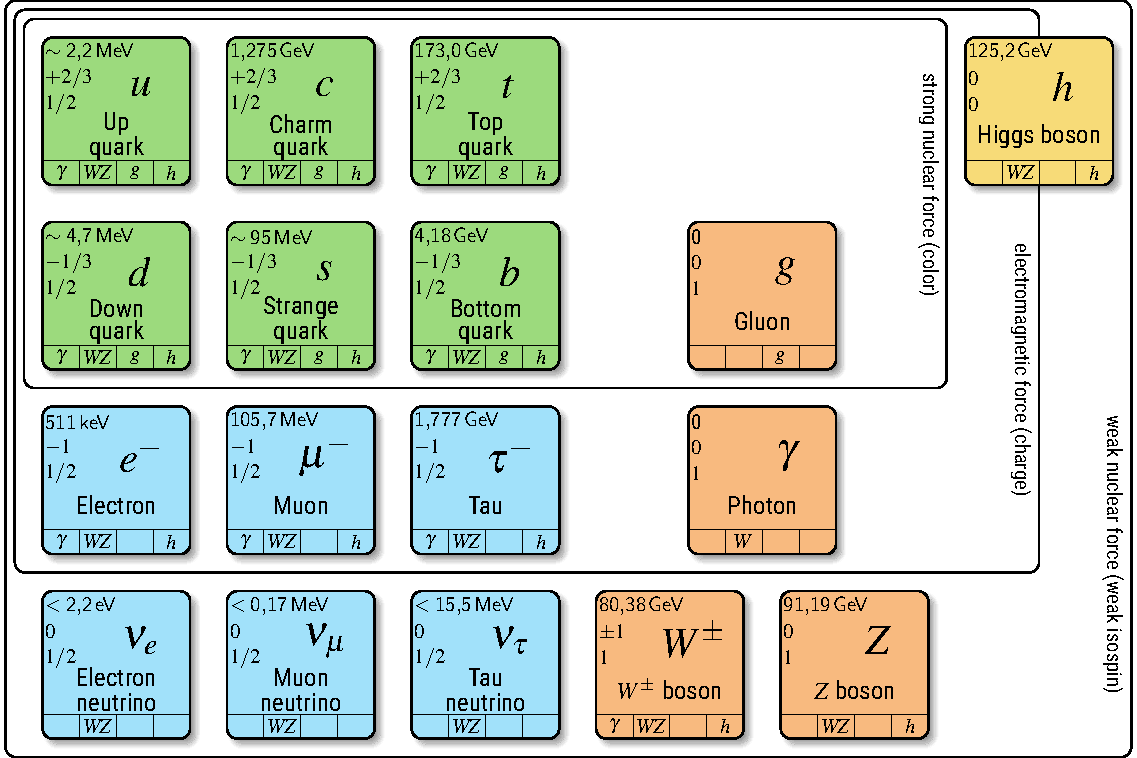
\includegraphics[height=\graphh]{\PhDthesisdir/plots_and_images/Particles_tables/SM2018_EN_for_slides.pdf}
\vspace{-5pt}
\end{center}
\end{frame}

\begin{frame}
\frametitle{Higgs boson in the Standard Model}

\begin{minipage}[c]{.45\textwidth}
\begin{equation*}
\phi
=
\begin{pmatrix}
\phi^+ \\ \phi^0
\end{pmatrix}
=
\frac{1}{\sqrt{2}}
\begin{pmatrix}
\phi_3 + \im \phi_4 \\ \phi_1 + \im \phi_2
\end{pmatrix}
\end{equation*}

\begin{equation*}
V(\phi)
= \mu^2\phi^\dagger\phi + \lambda (\phi^\dagger\phi)^2
\msep \lambda > 0
\end{equation*}

\begin{equation*}
\average{\phi}_0 = \frac{v}{\sqrt{2}} = \sqrt{\frac{-\mu^2}{2\lambda}} \neq 0
\end{equation*}

\begin{equation*}
\phi(x)
=
\frac{1}{\sqrt{2}}
\begin{pmatrix}
0 \\ v + \higgs(x)
\end{pmatrix}
\end{equation*}

\end{minipage}
\begin{minipage}[c]{.5\textwidth}
\vspace{-20pt}
%% Creator: Matplotlib, PGF backend
%%
%% To include the figure in your LaTeX document, write
%%   \input{<filename>.pgf}
%%
%% Make sure the required packages are loaded in your preamble
%%   \usepackage{pgf}
%%
%% Figures using additional raster images can only be included by \input if
%% they are in the same directory as the main LaTeX file. For loading figures
%% from other directories you can use the `import` package
%%   \usepackage{import}
%% and then include the figures with
%%   \import{<path to file>}{<filename>.pgf}
%%
%% Matplotlib used the following preamble
%%   \usepackage[utf8x]{inputenc}
%%   \usepackage[T1]{fontenc}
%%   \usepackage{sistyle}
%%   \SIproductsign{\!\times\!}\SIunitsep{\,}\SIunitdot{{\fontfamily{cmr}\cdot}}
%%   \SIdecimalsign{,}\SIthousandsep{\,}
%%
\begingroup%
\makeatletter%
\begin{pgfpicture}%
\pgfpathrectangle{\pgfpointorigin}{\pgfqpoint{3.011811in}{3.011811in}}%
\pgfusepath{use as bounding box, clip}%
\begin{pgfscope}%
\pgfsetbuttcap%
\pgfsetmiterjoin%
\definecolor{currentfill}{rgb}{1.000000,1.000000,1.000000}%
\pgfsetfillcolor{currentfill}%
\pgfsetlinewidth{0.000000pt}%
\definecolor{currentstroke}{rgb}{1.000000,1.000000,1.000000}%
\pgfsetstrokecolor{currentstroke}%
\pgfsetdash{}{0pt}%
\pgfpathmoveto{\pgfqpoint{0.000000in}{0.000000in}}%
\pgfpathlineto{\pgfqpoint{3.011811in}{0.000000in}}%
\pgfpathlineto{\pgfqpoint{3.011811in}{3.011811in}}%
\pgfpathlineto{\pgfqpoint{0.000000in}{3.011811in}}%
\pgfpathclose%
\pgfusepath{fill}%
\end{pgfscope}%
\begin{pgfscope}%
\pgfsetbuttcap%
\pgfsetmiterjoin%
\definecolor{currentfill}{rgb}{1.000000,1.000000,1.000000}%
\pgfsetfillcolor{currentfill}%
\pgfsetlinewidth{0.000000pt}%
\definecolor{currentstroke}{rgb}{0.000000,0.000000,0.000000}%
\pgfsetstrokecolor{currentstroke}%
\pgfsetstrokeopacity{0.000000}%
\pgfsetdash{}{0pt}%
\pgfpathmoveto{\pgfqpoint{0.384006in}{0.331299in}}%
\pgfpathlineto{\pgfqpoint{2.703100in}{0.331299in}}%
\pgfpathlineto{\pgfqpoint{2.703100in}{2.650394in}}%
\pgfpathlineto{\pgfqpoint{0.384006in}{2.650394in}}%
\pgfpathclose%
\pgfusepath{fill}%
\end{pgfscope}%
\begin{pgfscope}%
\pgfsetbuttcap%
\pgfsetmiterjoin%
\definecolor{currentfill}{rgb}{0.950000,0.950000,0.950000}%
\pgfsetfillcolor{currentfill}%
\pgfsetfillopacity{0.500000}%
\pgfsetlinewidth{1.003750pt}%
\definecolor{currentstroke}{rgb}{0.950000,0.950000,0.950000}%
\pgfsetstrokecolor{currentstroke}%
\pgfsetstrokeopacity{0.500000}%
\pgfsetdash{}{0pt}%
\pgfpathmoveto{\pgfqpoint{0.691438in}{0.843737in}}%
\pgfpathlineto{\pgfqpoint{1.355175in}{1.412327in}}%
\pgfpathlineto{\pgfqpoint{1.344124in}{2.498808in}}%
\pgfpathlineto{\pgfqpoint{0.643380in}{1.987942in}}%
\pgfusepath{stroke,fill}%
\end{pgfscope}%
\begin{pgfscope}%
\pgfsetbuttcap%
\pgfsetmiterjoin%
\definecolor{currentfill}{rgb}{0.900000,0.900000,0.900000}%
\pgfsetfillcolor{currentfill}%
\pgfsetfillopacity{0.500000}%
\pgfsetlinewidth{1.003750pt}%
\definecolor{currentstroke}{rgb}{0.900000,0.900000,0.900000}%
\pgfsetstrokecolor{currentstroke}%
\pgfsetstrokeopacity{0.500000}%
\pgfsetdash{}{0pt}%
\pgfpathmoveto{\pgfqpoint{1.355175in}{1.412327in}}%
\pgfpathlineto{\pgfqpoint{2.430366in}{1.094449in}}%
\pgfpathlineto{\pgfqpoint{2.475351in}{2.213692in}}%
\pgfpathlineto{\pgfqpoint{1.344124in}{2.498808in}}%
\pgfusepath{stroke,fill}%
\end{pgfscope}%
\begin{pgfscope}%
\pgfsetbuttcap%
\pgfsetmiterjoin%
\definecolor{currentfill}{rgb}{0.925000,0.925000,0.925000}%
\pgfsetfillcolor{currentfill}%
\pgfsetfillopacity{0.500000}%
\pgfsetlinewidth{1.003750pt}%
\definecolor{currentstroke}{rgb}{0.925000,0.925000,0.925000}%
\pgfsetstrokecolor{currentstroke}%
\pgfsetstrokeopacity{0.500000}%
\pgfsetdash{}{0pt}%
\pgfpathmoveto{\pgfqpoint{0.691438in}{0.843737in}}%
\pgfpathlineto{\pgfqpoint{1.822684in}{0.473516in}}%
\pgfpathlineto{\pgfqpoint{2.430366in}{1.094449in}}%
\pgfpathlineto{\pgfqpoint{1.355175in}{1.412327in}}%
\pgfusepath{stroke,fill}%
\end{pgfscope}%
\begin{pgfscope}%
\pgfsetrectcap%
\pgfsetroundjoin%
\pgfsetlinewidth{0.803000pt}%
\definecolor{currentstroke}{rgb}{0.000000,0.000000,0.000000}%
\pgfsetstrokecolor{currentstroke}%
\pgfsetdash{}{0pt}%
\pgfpathmoveto{\pgfqpoint{0.691438in}{0.843737in}}%
\pgfpathlineto{\pgfqpoint{1.822684in}{0.473516in}}%
\pgfusepath{stroke}%
\end{pgfscope}%
\begin{pgfscope}%
\definecolor{textcolor}{rgb}{0.000000,0.000000,0.000000}%
\pgfsetstrokecolor{textcolor}%
\pgfsetfillcolor{textcolor}%
\pgftext[x=0.900866in,y=0.170722in,left,base,rotate=341.878381]{\color{textcolor}\rmfamily\fontsize{10.000000}{12.000000}\selectfont \(\displaystyle \Re(\phi)\)}%
\end{pgfscope}%
\begin{pgfscope}%
\pgfsetbuttcap%
\pgfsetroundjoin%
\pgfsetlinewidth{0.803000pt}%
\definecolor{currentstroke}{rgb}{0.690196,0.690196,0.690196}%
\pgfsetstrokecolor{currentstroke}%
\pgfsetdash{}{0pt}%
\pgfpathmoveto{\pgfqpoint{1.243629in}{0.663023in}}%
\pgfpathlineto{\pgfqpoint{1.880905in}{1.256896in}}%
\pgfpathlineto{\pgfqpoint{1.896638in}{2.359552in}}%
\pgfusepath{stroke}%
\end{pgfscope}%
\begin{pgfscope}%
\pgfsetrectcap%
\pgfsetroundjoin%
\pgfsetlinewidth{0.803000pt}%
\definecolor{currentstroke}{rgb}{0.000000,0.000000,0.000000}%
\pgfsetstrokecolor{currentstroke}%
\pgfsetdash{}{0pt}%
\pgfpathmoveto{\pgfqpoint{1.249128in}{0.668146in}}%
\pgfpathlineto{\pgfqpoint{1.232612in}{0.652756in}}%
\pgfusepath{stroke}%
\end{pgfscope}%
\begin{pgfscope}%
\definecolor{textcolor}{rgb}{0.000000,0.000000,0.000000}%
\pgfsetstrokecolor{textcolor}%
\pgfsetfillcolor{textcolor}%
\pgftext[x=1.154690in,y=0.431956in,,top]{\color{textcolor}\rmfamily\fontsize{9.000000}{10.800000}\selectfont \num{0}}%
\end{pgfscope}%
\begin{pgfscope}%
\pgfsetrectcap%
\pgfsetroundjoin%
\pgfsetlinewidth{0.803000pt}%
\definecolor{currentstroke}{rgb}{0.000000,0.000000,0.000000}%
\pgfsetstrokecolor{currentstroke}%
\pgfsetdash{}{0pt}%
\pgfpathmoveto{\pgfqpoint{2.430366in}{1.094449in}}%
\pgfpathlineto{\pgfqpoint{1.822684in}{0.473516in}}%
\pgfusepath{stroke}%
\end{pgfscope}%
\begin{pgfscope}%
\definecolor{textcolor}{rgb}{0.000000,0.000000,0.000000}%
\pgfsetstrokecolor{textcolor}%
\pgfsetfillcolor{textcolor}%
\pgftext[x=2.383553in,y=0.252572in,left,base,rotate=45.617904]{\color{textcolor}\rmfamily\fontsize{10.000000}{12.000000}\selectfont \(\displaystyle \Im(\phi)\)}%
\end{pgfscope}%
\begin{pgfscope}%
\pgfsetbuttcap%
\pgfsetroundjoin%
\pgfsetlinewidth{0.803000pt}%
\definecolor{currentstroke}{rgb}{0.690196,0.690196,0.690196}%
\pgfsetstrokecolor{currentstroke}%
\pgfsetdash{}{0pt}%
\pgfpathmoveto{\pgfqpoint{1.007486in}{2.253388in}}%
\pgfpathlineto{\pgfqpoint{1.035669in}{1.138623in}}%
\pgfpathlineto{\pgfqpoint{2.138353in}{0.796068in}}%
\pgfusepath{stroke}%
\end{pgfscope}%
\begin{pgfscope}%
\pgfsetrectcap%
\pgfsetroundjoin%
\pgfsetlinewidth{0.803000pt}%
\definecolor{currentstroke}{rgb}{0.000000,0.000000,0.000000}%
\pgfsetstrokecolor{currentstroke}%
\pgfsetdash{}{0pt}%
\pgfpathmoveto{\pgfqpoint{2.129138in}{0.798931in}}%
\pgfpathlineto{\pgfqpoint{2.156802in}{0.790337in}}%
\pgfusepath{stroke}%
\end{pgfscope}%
\begin{pgfscope}%
\definecolor{textcolor}{rgb}{0.000000,0.000000,0.000000}%
\pgfsetstrokecolor{textcolor}%
\pgfsetfillcolor{textcolor}%
\pgftext[x=2.286717in,y=0.604874in,,top]{\color{textcolor}\rmfamily\fontsize{9.000000}{10.800000}\selectfont \num{0}}%
\end{pgfscope}%
\begin{pgfscope}%
\pgfsetrectcap%
\pgfsetroundjoin%
\pgfsetlinewidth{0.803000pt}%
\definecolor{currentstroke}{rgb}{0.000000,0.000000,0.000000}%
\pgfsetstrokecolor{currentstroke}%
\pgfsetdash{}{0pt}%
\pgfpathmoveto{\pgfqpoint{2.430366in}{1.094449in}}%
\pgfpathlineto{\pgfqpoint{2.475351in}{2.213692in}}%
\pgfusepath{stroke}%
\end{pgfscope}%
\begin{pgfscope}%
\pgfsetbuttcap%
\pgfsetroundjoin%
\pgfsetlinewidth{0.803000pt}%
\definecolor{currentstroke}{rgb}{0.690196,0.690196,0.690196}%
\pgfsetstrokecolor{currentstroke}%
\pgfsetdash{}{0pt}%
\pgfpathmoveto{\pgfqpoint{2.452972in}{1.656887in}}%
\pgfpathlineto{\pgfqpoint{1.349616in}{1.958893in}}%
\pgfpathlineto{\pgfqpoint{0.667308in}{1.418227in}}%
\pgfusepath{stroke}%
\end{pgfscope}%
\begin{pgfscope}%
\pgfsetrectcap%
\pgfsetroundjoin%
\pgfsetlinewidth{0.803000pt}%
\definecolor{currentstroke}{rgb}{0.000000,0.000000,0.000000}%
\pgfsetstrokecolor{currentstroke}%
\pgfsetdash{}{0pt}%
\pgfpathmoveto{\pgfqpoint{2.443756in}{1.659410in}}%
\pgfpathlineto{\pgfqpoint{2.471423in}{1.651837in}}%
\pgfusepath{stroke}%
\end{pgfscope}%
\begin{pgfscope}%
\definecolor{textcolor}{rgb}{0.000000,0.000000,0.000000}%
\pgfsetstrokecolor{textcolor}%
\pgfsetfillcolor{textcolor}%
\pgftext[x=2.680446in,y=1.687290in,,top]{\color{textcolor}\rmfamily\fontsize{9.000000}{10.800000}\selectfont \num{0}}%
\end{pgfscope}%
\begin{pgfscope}%
\pgfpathrectangle{\pgfqpoint{0.384006in}{0.331299in}}{\pgfqpoint{2.319094in}{2.319094in}}%
\pgfusepath{clip}%
\pgfsetrectcap%
\pgfsetroundjoin%
\pgfsetlinewidth{1.505625pt}%
\definecolor{currentstroke}{rgb}{1.000000,1.000000,1.000000}%
\pgfsetstrokecolor{currentstroke}%
\pgfsetdash{}{0pt}%
\pgfpathmoveto{\pgfqpoint{0.804686in}{0.881877in}}%
\pgfusepath{stroke}%
\end{pgfscope}%
\begin{pgfscope}%
\pgfpathrectangle{\pgfqpoint{0.384006in}{0.331299in}}{\pgfqpoint{2.319094in}{2.319094in}}%
\pgfusepath{clip}%
\pgfsetrectcap%
\pgfsetroundjoin%
\pgfsetlinewidth{1.505625pt}%
\definecolor{currentstroke}{rgb}{1.000000,1.000000,1.000000}%
\pgfsetstrokecolor{currentstroke}%
\pgfsetdash{}{0pt}%
\pgfpathmoveto{\pgfqpoint{0.784509in}{1.433891in}}%
\pgfusepath{stroke}%
\end{pgfscope}%
\begin{pgfscope}%
\pgfpathrectangle{\pgfqpoint{0.384006in}{0.331299in}}{\pgfqpoint{2.319094in}{2.319094in}}%
\pgfusepath{clip}%
\pgfsetrectcap%
\pgfsetroundjoin%
\pgfsetlinewidth{1.505625pt}%
\definecolor{currentstroke}{rgb}{1.000000,1.000000,1.000000}%
\pgfsetstrokecolor{currentstroke}%
\pgfsetdash{}{0pt}%
\pgfpathmoveto{\pgfqpoint{1.381560in}{1.379776in}}%
\pgfusepath{stroke}%
\end{pgfscope}%
\begin{pgfscope}%
\pgfpathrectangle{\pgfqpoint{0.384006in}{0.331299in}}{\pgfqpoint{2.319094in}{2.319094in}}%
\pgfusepath{clip}%
\pgfsetrectcap%
\pgfsetroundjoin%
\pgfsetlinewidth{1.505625pt}%
\definecolor{currentstroke}{rgb}{1.000000,1.000000,1.000000}%
\pgfsetstrokecolor{currentstroke}%
\pgfsetdash{}{0pt}%
\pgfpathmoveto{\pgfqpoint{1.376823in}{1.908245in}}%
\pgfusepath{stroke}%
\end{pgfscope}%
\begin{pgfscope}%
\pgfpathrectangle{\pgfqpoint{0.384006in}{0.331299in}}{\pgfqpoint{2.319094in}{2.319094in}}%
\pgfusepath{clip}%
\pgfsetrectcap%
\pgfsetroundjoin%
\pgfsetlinewidth{1.505625pt}%
\definecolor{currentstroke}{rgb}{1.000000,1.000000,1.000000}%
\pgfsetstrokecolor{currentstroke}%
\pgfsetdash{}{0pt}%
\pgfpathmoveto{\pgfqpoint{1.789633in}{0.562583in}}%
\pgfusepath{stroke}%
\end{pgfscope}%
\begin{pgfscope}%
\pgfpathrectangle{\pgfqpoint{0.384006in}{0.331299in}}{\pgfqpoint{2.319094in}{2.319094in}}%
\pgfusepath{clip}%
\pgfsetrectcap%
\pgfsetroundjoin%
\pgfsetlinewidth{1.505625pt}%
\definecolor{currentstroke}{rgb}{1.000000,1.000000,1.000000}%
\pgfsetstrokecolor{currentstroke}%
\pgfsetdash{}{0pt}%
\pgfpathmoveto{\pgfqpoint{1.795493in}{1.128869in}}%
\pgfusepath{stroke}%
\end{pgfscope}%
\begin{pgfscope}%
\pgfpathrectangle{\pgfqpoint{0.384006in}{0.331299in}}{\pgfqpoint{2.319094in}{2.319094in}}%
\pgfusepath{clip}%
\pgfsetrectcap%
\pgfsetroundjoin%
\pgfsetlinewidth{1.505625pt}%
\definecolor{currentstroke}{rgb}{1.000000,1.000000,1.000000}%
\pgfsetstrokecolor{currentstroke}%
\pgfsetdash{}{0pt}%
\pgfpathmoveto{\pgfqpoint{2.323745in}{1.100284in}}%
\pgfusepath{stroke}%
\end{pgfscope}%
\begin{pgfscope}%
\pgfpathrectangle{\pgfqpoint{0.384006in}{0.331299in}}{\pgfqpoint{2.319094in}{2.319094in}}%
\pgfusepath{clip}%
\pgfsetrectcap%
\pgfsetroundjoin%
\pgfsetlinewidth{1.505625pt}%
\definecolor{currentstroke}{rgb}{1.000000,1.000000,1.000000}%
\pgfsetstrokecolor{currentstroke}%
\pgfsetdash{}{0pt}%
\pgfpathmoveto{\pgfqpoint{2.342805in}{1.642163in}}%
\pgfusepath{stroke}%
\end{pgfscope}%
\begin{pgfscope}%
\pgfpathrectangle{\pgfqpoint{0.384006in}{0.331299in}}{\pgfqpoint{2.319094in}{2.319094in}}%
\pgfusepath{clip}%
\pgfsetbuttcap%
\pgfsetroundjoin%
\definecolor{currentfill}{rgb}{0.271104,0.360011,0.807095}%
\pgfsetfillcolor{currentfill}%
\pgfsetfillopacity{0.700000}%
\pgfsetlinewidth{1.003750pt}%
\definecolor{currentstroke}{rgb}{0.271104,0.360011,0.807095}%
\pgfsetstrokecolor{currentstroke}%
\pgfsetstrokeopacity{0.700000}%
\pgfsetdash{}{0pt}%
\pgfpathmoveto{\pgfqpoint{1.595532in}{1.294116in}}%
\pgfpathlineto{\pgfqpoint{1.596002in}{1.317278in}}%
\pgfpathlineto{\pgfqpoint{1.531271in}{1.316567in}}%
\pgfpathlineto{\pgfqpoint{1.532211in}{1.293418in}}%
\pgfpathclose%
\pgfusepath{stroke,fill}%
\end{pgfscope}%
\begin{pgfscope}%
\pgfpathrectangle{\pgfqpoint{0.384006in}{0.331299in}}{\pgfqpoint{2.319094in}{2.319094in}}%
\pgfusepath{clip}%
\pgfsetbuttcap%
\pgfsetroundjoin%
\definecolor{currentfill}{rgb}{0.252663,0.332837,0.783665}%
\pgfsetfillcolor{currentfill}%
\pgfsetfillopacity{0.700000}%
\pgfsetlinewidth{1.003750pt}%
\definecolor{currentstroke}{rgb}{0.252663,0.332837,0.783665}%
\pgfsetstrokecolor{currentstroke}%
\pgfsetstrokeopacity{0.700000}%
\pgfsetdash{}{0pt}%
\pgfpathmoveto{\pgfqpoint{1.595065in}{1.274612in}}%
\pgfpathlineto{\pgfqpoint{1.595532in}{1.294116in}}%
\pgfpathlineto{\pgfqpoint{1.532211in}{1.293418in}}%
\pgfpathlineto{\pgfqpoint{1.533145in}{1.273928in}}%
\pgfpathclose%
\pgfusepath{stroke,fill}%
\end{pgfscope}%
\begin{pgfscope}%
\pgfpathrectangle{\pgfqpoint{0.384006in}{0.331299in}}{\pgfqpoint{2.319094in}{2.319094in}}%
\pgfusepath{clip}%
\pgfsetbuttcap%
\pgfsetroundjoin%
\definecolor{currentfill}{rgb}{0.289996,0.386836,0.828926}%
\pgfsetfillcolor{currentfill}%
\pgfsetfillopacity{0.700000}%
\pgfsetlinewidth{1.003750pt}%
\definecolor{currentstroke}{rgb}{0.289996,0.386836,0.828926}%
\pgfsetstrokecolor{currentstroke}%
\pgfsetstrokeopacity{0.700000}%
\pgfsetdash{}{0pt}%
\pgfpathmoveto{\pgfqpoint{1.596002in}{1.317278in}}%
\pgfpathlineto{\pgfqpoint{1.596477in}{1.344334in}}%
\pgfpathlineto{\pgfqpoint{1.530322in}{1.343609in}}%
\pgfpathlineto{\pgfqpoint{1.531271in}{1.316567in}}%
\pgfpathclose%
\pgfusepath{stroke,fill}%
\end{pgfscope}%
\begin{pgfscope}%
\pgfpathrectangle{\pgfqpoint{0.384006in}{0.331299in}}{\pgfqpoint{2.319094in}{2.319094in}}%
\pgfusepath{clip}%
\pgfsetbuttcap%
\pgfsetroundjoin%
\definecolor{currentfill}{rgb}{0.271104,0.360011,0.807095}%
\pgfsetfillcolor{currentfill}%
\pgfsetfillopacity{0.700000}%
\pgfsetlinewidth{1.003750pt}%
\definecolor{currentstroke}{rgb}{0.271104,0.360011,0.807095}%
\pgfsetstrokecolor{currentstroke}%
\pgfsetstrokeopacity{0.700000}%
\pgfsetdash{}{0pt}%
\pgfpathmoveto{\pgfqpoint{1.658541in}{1.290631in}}%
\pgfpathlineto{\pgfqpoint{1.660416in}{1.313726in}}%
\pgfpathlineto{\pgfqpoint{1.596002in}{1.317278in}}%
\pgfpathlineto{\pgfqpoint{1.595532in}{1.294116in}}%
\pgfpathclose%
\pgfusepath{stroke,fill}%
\end{pgfscope}%
\begin{pgfscope}%
\pgfpathrectangle{\pgfqpoint{0.384006in}{0.331299in}}{\pgfqpoint{2.319094in}{2.319094in}}%
\pgfusepath{clip}%
\pgfsetbuttcap%
\pgfsetroundjoin%
\definecolor{currentfill}{rgb}{0.252663,0.332837,0.783665}%
\pgfsetfillcolor{currentfill}%
\pgfsetfillopacity{0.700000}%
\pgfsetlinewidth{1.003750pt}%
\definecolor{currentstroke}{rgb}{0.252663,0.332837,0.783665}%
\pgfsetstrokecolor{currentstroke}%
\pgfsetstrokeopacity{0.700000}%
\pgfsetdash{}{0pt}%
\pgfpathmoveto{\pgfqpoint{1.656680in}{1.271195in}}%
\pgfpathlineto{\pgfqpoint{1.658541in}{1.290631in}}%
\pgfpathlineto{\pgfqpoint{1.595532in}{1.294116in}}%
\pgfpathlineto{\pgfqpoint{1.595065in}{1.274612in}}%
\pgfpathclose%
\pgfusepath{stroke,fill}%
\end{pgfscope}%
\begin{pgfscope}%
\pgfpathrectangle{\pgfqpoint{0.384006in}{0.331299in}}{\pgfqpoint{2.319094in}{2.319094in}}%
\pgfusepath{clip}%
\pgfsetbuttcap%
\pgfsetroundjoin%
\definecolor{currentfill}{rgb}{0.243520,0.319189,0.771672}%
\pgfsetfillcolor{currentfill}%
\pgfsetfillopacity{0.700000}%
\pgfsetlinewidth{1.003750pt}%
\definecolor{currentstroke}{rgb}{0.243520,0.319189,0.771672}%
\pgfsetstrokecolor{currentstroke}%
\pgfsetstrokeopacity{0.700000}%
\pgfsetdash{}{0pt}%
\pgfpathmoveto{\pgfqpoint{1.594601in}{1.258540in}}%
\pgfpathlineto{\pgfqpoint{1.595065in}{1.274612in}}%
\pgfpathlineto{\pgfqpoint{1.533145in}{1.273928in}}%
\pgfpathlineto{\pgfqpoint{1.534071in}{1.257869in}}%
\pgfpathclose%
\pgfusepath{stroke,fill}%
\end{pgfscope}%
\begin{pgfscope}%
\pgfpathrectangle{\pgfqpoint{0.384006in}{0.331299in}}{\pgfqpoint{2.319094in}{2.319094in}}%
\pgfusepath{clip}%
\pgfsetbuttcap%
\pgfsetroundjoin%
\definecolor{currentfill}{rgb}{0.289996,0.386836,0.828926}%
\pgfsetfillcolor{currentfill}%
\pgfsetfillopacity{0.700000}%
\pgfsetlinewidth{1.003750pt}%
\definecolor{currentstroke}{rgb}{0.289996,0.386836,0.828926}%
\pgfsetstrokecolor{currentstroke}%
\pgfsetstrokeopacity{0.700000}%
\pgfsetdash{}{0pt}%
\pgfpathmoveto{\pgfqpoint{1.660416in}{1.313726in}}%
\pgfpathlineto{\pgfqpoint{1.662307in}{1.340717in}}%
\pgfpathlineto{\pgfqpoint{1.596477in}{1.344334in}}%
\pgfpathlineto{\pgfqpoint{1.596002in}{1.317278in}}%
\pgfpathclose%
\pgfusepath{stroke,fill}%
\end{pgfscope}%
\begin{pgfscope}%
\pgfpathrectangle{\pgfqpoint{0.384006in}{0.331299in}}{\pgfqpoint{2.319094in}{2.319094in}}%
\pgfusepath{clip}%
\pgfsetbuttcap%
\pgfsetroundjoin%
\definecolor{currentfill}{rgb}{0.271104,0.360011,0.807095}%
\pgfsetfillcolor{currentfill}%
\pgfsetfillopacity{0.700000}%
\pgfsetlinewidth{1.003750pt}%
\definecolor{currentstroke}{rgb}{0.271104,0.360011,0.807095}%
\pgfsetstrokecolor{currentstroke}%
\pgfsetstrokeopacity{0.700000}%
\pgfsetdash{}{0pt}%
\pgfpathmoveto{\pgfqpoint{1.532211in}{1.293418in}}%
\pgfpathlineto{\pgfqpoint{1.531271in}{1.316567in}}%
\pgfpathlineto{\pgfqpoint{1.467174in}{1.311601in}}%
\pgfpathlineto{\pgfqpoint{1.469513in}{1.288546in}}%
\pgfpathclose%
\pgfusepath{stroke,fill}%
\end{pgfscope}%
\begin{pgfscope}%
\pgfpathrectangle{\pgfqpoint{0.384006in}{0.331299in}}{\pgfqpoint{2.319094in}{2.319094in}}%
\pgfusepath{clip}%
\pgfsetbuttcap%
\pgfsetroundjoin%
\definecolor{currentfill}{rgb}{0.252663,0.332837,0.783665}%
\pgfsetfillcolor{currentfill}%
\pgfsetfillopacity{0.700000}%
\pgfsetlinewidth{1.003750pt}%
\definecolor{currentstroke}{rgb}{0.252663,0.332837,0.783665}%
\pgfsetstrokecolor{currentstroke}%
\pgfsetstrokeopacity{0.700000}%
\pgfsetdash{}{0pt}%
\pgfpathmoveto{\pgfqpoint{1.533145in}{1.273928in}}%
\pgfpathlineto{\pgfqpoint{1.532211in}{1.293418in}}%
\pgfpathlineto{\pgfqpoint{1.469513in}{1.288546in}}%
\pgfpathlineto{\pgfqpoint{1.471834in}{1.269151in}}%
\pgfpathclose%
\pgfusepath{stroke,fill}%
\end{pgfscope}%
\begin{pgfscope}%
\pgfpathrectangle{\pgfqpoint{0.384006in}{0.331299in}}{\pgfqpoint{2.319094in}{2.319094in}}%
\pgfusepath{clip}%
\pgfsetbuttcap%
\pgfsetroundjoin%
\definecolor{currentfill}{rgb}{0.243520,0.319189,0.771672}%
\pgfsetfillcolor{currentfill}%
\pgfsetfillopacity{0.700000}%
\pgfsetlinewidth{1.003750pt}%
\definecolor{currentstroke}{rgb}{0.243520,0.319189,0.771672}%
\pgfsetstrokecolor{currentstroke}%
\pgfsetstrokeopacity{0.700000}%
\pgfsetdash{}{0pt}%
\pgfpathmoveto{\pgfqpoint{1.654831in}{1.255192in}}%
\pgfpathlineto{\pgfqpoint{1.656680in}{1.271195in}}%
\pgfpathlineto{\pgfqpoint{1.595065in}{1.274612in}}%
\pgfpathlineto{\pgfqpoint{1.594601in}{1.258540in}}%
\pgfpathclose%
\pgfusepath{stroke,fill}%
\end{pgfscope}%
\begin{pgfscope}%
\pgfpathrectangle{\pgfqpoint{0.384006in}{0.331299in}}{\pgfqpoint{2.319094in}{2.319094in}}%
\pgfusepath{clip}%
\pgfsetbuttcap%
\pgfsetroundjoin%
\definecolor{currentfill}{rgb}{0.318832,0.426605,0.859857}%
\pgfsetfillcolor{currentfill}%
\pgfsetfillopacity{0.700000}%
\pgfsetlinewidth{1.003750pt}%
\definecolor{currentstroke}{rgb}{0.318832,0.426605,0.859857}%
\pgfsetstrokecolor{currentstroke}%
\pgfsetstrokeopacity{0.700000}%
\pgfsetdash{}{0pt}%
\pgfpathmoveto{\pgfqpoint{1.596477in}{1.344334in}}%
\pgfpathlineto{\pgfqpoint{1.596956in}{1.375530in}}%
\pgfpathlineto{\pgfqpoint{1.529365in}{1.374793in}}%
\pgfpathlineto{\pgfqpoint{1.530322in}{1.343609in}}%
\pgfpathclose%
\pgfusepath{stroke,fill}%
\end{pgfscope}%
\begin{pgfscope}%
\pgfpathrectangle{\pgfqpoint{0.384006in}{0.331299in}}{\pgfqpoint{2.319094in}{2.319094in}}%
\pgfusepath{clip}%
\pgfsetbuttcap%
\pgfsetroundjoin%
\definecolor{currentfill}{rgb}{0.289996,0.386836,0.828926}%
\pgfsetfillcolor{currentfill}%
\pgfsetfillopacity{0.700000}%
\pgfsetlinewidth{1.003750pt}%
\definecolor{currentstroke}{rgb}{0.289996,0.386836,0.828926}%
\pgfsetstrokecolor{currentstroke}%
\pgfsetstrokeopacity{0.700000}%
\pgfsetdash{}{0pt}%
\pgfpathmoveto{\pgfqpoint{1.531271in}{1.316567in}}%
\pgfpathlineto{\pgfqpoint{1.530322in}{1.343609in}}%
\pgfpathlineto{\pgfqpoint{1.464815in}{1.338553in}}%
\pgfpathlineto{\pgfqpoint{1.467174in}{1.311601in}}%
\pgfpathclose%
\pgfusepath{stroke,fill}%
\end{pgfscope}%
\begin{pgfscope}%
\pgfpathrectangle{\pgfqpoint{0.384006in}{0.331299in}}{\pgfqpoint{2.319094in}{2.319094in}}%
\pgfusepath{clip}%
\pgfsetbuttcap%
\pgfsetroundjoin%
\definecolor{currentfill}{rgb}{0.234377,0.305542,0.759680}%
\pgfsetfillcolor{currentfill}%
\pgfsetfillopacity{0.700000}%
\pgfsetlinewidth{1.003750pt}%
\definecolor{currentstroke}{rgb}{0.234377,0.305542,0.759680}%
\pgfsetstrokecolor{currentstroke}%
\pgfsetstrokeopacity{0.700000}%
\pgfsetdash{}{0pt}%
\pgfpathmoveto{\pgfqpoint{1.594140in}{1.245680in}}%
\pgfpathlineto{\pgfqpoint{1.594601in}{1.258540in}}%
\pgfpathlineto{\pgfqpoint{1.534071in}{1.257869in}}%
\pgfpathlineto{\pgfqpoint{1.534993in}{1.245024in}}%
\pgfpathclose%
\pgfusepath{stroke,fill}%
\end{pgfscope}%
\begin{pgfscope}%
\pgfpathrectangle{\pgfqpoint{0.384006in}{0.331299in}}{\pgfqpoint{2.319094in}{2.319094in}}%
\pgfusepath{clip}%
\pgfsetbuttcap%
\pgfsetroundjoin%
\definecolor{currentfill}{rgb}{0.243520,0.319189,0.771672}%
\pgfsetfillcolor{currentfill}%
\pgfsetfillopacity{0.700000}%
\pgfsetlinewidth{1.003750pt}%
\definecolor{currentstroke}{rgb}{0.243520,0.319189,0.771672}%
\pgfsetstrokecolor{currentstroke}%
\pgfsetstrokeopacity{0.700000}%
\pgfsetdash{}{0pt}%
\pgfpathmoveto{\pgfqpoint{1.534071in}{1.257869in}}%
\pgfpathlineto{\pgfqpoint{1.533145in}{1.273928in}}%
\pgfpathlineto{\pgfqpoint{1.471834in}{1.269151in}}%
\pgfpathlineto{\pgfqpoint{1.474140in}{1.253190in}}%
\pgfpathclose%
\pgfusepath{stroke,fill}%
\end{pgfscope}%
\begin{pgfscope}%
\pgfpathrectangle{\pgfqpoint{0.384006in}{0.331299in}}{\pgfqpoint{2.319094in}{2.319094in}}%
\pgfusepath{clip}%
\pgfsetbuttcap%
\pgfsetroundjoin%
\definecolor{currentfill}{rgb}{0.318832,0.426605,0.859857}%
\pgfsetfillcolor{currentfill}%
\pgfsetfillopacity{0.700000}%
\pgfsetlinewidth{1.003750pt}%
\definecolor{currentstroke}{rgb}{0.318832,0.426605,0.859857}%
\pgfsetstrokecolor{currentstroke}%
\pgfsetstrokeopacity{0.700000}%
\pgfsetdash{}{0pt}%
\pgfpathmoveto{\pgfqpoint{1.662307in}{1.340717in}}%
\pgfpathlineto{\pgfqpoint{1.664216in}{1.371851in}}%
\pgfpathlineto{\pgfqpoint{1.596956in}{1.375530in}}%
\pgfpathlineto{\pgfqpoint{1.596477in}{1.344334in}}%
\pgfpathclose%
\pgfusepath{stroke,fill}%
\end{pgfscope}%
\begin{pgfscope}%
\pgfpathrectangle{\pgfqpoint{0.384006in}{0.331299in}}{\pgfqpoint{2.319094in}{2.319094in}}%
\pgfusepath{clip}%
\pgfsetbuttcap%
\pgfsetroundjoin%
\definecolor{currentfill}{rgb}{0.234377,0.305542,0.759680}%
\pgfsetfillcolor{currentfill}%
\pgfsetfillopacity{0.700000}%
\pgfsetlinewidth{1.003750pt}%
\definecolor{currentstroke}{rgb}{0.234377,0.305542,0.759680}%
\pgfsetstrokecolor{currentstroke}%
\pgfsetstrokeopacity{0.700000}%
\pgfsetdash{}{0pt}%
\pgfpathmoveto{\pgfqpoint{1.652993in}{1.242403in}}%
\pgfpathlineto{\pgfqpoint{1.654831in}{1.255192in}}%
\pgfpathlineto{\pgfqpoint{1.594601in}{1.258540in}}%
\pgfpathlineto{\pgfqpoint{1.594140in}{1.245680in}}%
\pgfpathclose%
\pgfusepath{stroke,fill}%
\end{pgfscope}%
\begin{pgfscope}%
\pgfpathrectangle{\pgfqpoint{0.384006in}{0.331299in}}{\pgfqpoint{2.319094in}{2.319094in}}%
\pgfusepath{clip}%
\pgfsetbuttcap%
\pgfsetroundjoin%
\definecolor{currentfill}{rgb}{0.318832,0.426605,0.859857}%
\pgfsetfillcolor{currentfill}%
\pgfsetfillopacity{0.700000}%
\pgfsetlinewidth{1.003750pt}%
\definecolor{currentstroke}{rgb}{0.318832,0.426605,0.859857}%
\pgfsetstrokecolor{currentstroke}%
\pgfsetstrokeopacity{0.700000}%
\pgfsetdash{}{0pt}%
\pgfpathmoveto{\pgfqpoint{1.530322in}{1.343609in}}%
\pgfpathlineto{\pgfqpoint{1.529365in}{1.374793in}}%
\pgfpathlineto{\pgfqpoint{1.462433in}{1.369649in}}%
\pgfpathlineto{\pgfqpoint{1.464815in}{1.338553in}}%
\pgfpathclose%
\pgfusepath{stroke,fill}%
\end{pgfscope}%
\begin{pgfscope}%
\pgfpathrectangle{\pgfqpoint{0.384006in}{0.331299in}}{\pgfqpoint{2.319094in}{2.319094in}}%
\pgfusepath{clip}%
\pgfsetbuttcap%
\pgfsetroundjoin%
\definecolor{currentfill}{rgb}{0.234377,0.305542,0.759680}%
\pgfsetfillcolor{currentfill}%
\pgfsetfillopacity{0.700000}%
\pgfsetlinewidth{1.003750pt}%
\definecolor{currentstroke}{rgb}{0.234377,0.305542,0.759680}%
\pgfsetstrokecolor{currentstroke}%
\pgfsetstrokeopacity{0.700000}%
\pgfsetdash{}{0pt}%
\pgfpathmoveto{\pgfqpoint{1.534993in}{1.245024in}}%
\pgfpathlineto{\pgfqpoint{1.534071in}{1.257869in}}%
\pgfpathlineto{\pgfqpoint{1.474140in}{1.253190in}}%
\pgfpathlineto{\pgfqpoint{1.476431in}{1.240443in}}%
\pgfpathclose%
\pgfusepath{stroke,fill}%
\end{pgfscope}%
\begin{pgfscope}%
\pgfpathrectangle{\pgfqpoint{0.384006in}{0.331299in}}{\pgfqpoint{2.319094in}{2.319094in}}%
\pgfusepath{clip}%
\pgfsetbuttcap%
\pgfsetroundjoin%
\definecolor{currentfill}{rgb}{0.271104,0.360011,0.807095}%
\pgfsetfillcolor{currentfill}%
\pgfsetfillopacity{0.700000}%
\pgfsetlinewidth{1.003750pt}%
\definecolor{currentstroke}{rgb}{0.271104,0.360011,0.807095}%
\pgfsetstrokecolor{currentstroke}%
\pgfsetstrokeopacity{0.700000}%
\pgfsetdash{}{0pt}%
\pgfpathmoveto{\pgfqpoint{1.720307in}{1.283008in}}%
\pgfpathlineto{\pgfqpoint{1.723562in}{1.305957in}}%
\pgfpathlineto{\pgfqpoint{1.660416in}{1.313726in}}%
\pgfpathlineto{\pgfqpoint{1.658541in}{1.290631in}}%
\pgfpathclose%
\pgfusepath{stroke,fill}%
\end{pgfscope}%
\begin{pgfscope}%
\pgfpathrectangle{\pgfqpoint{0.384006in}{0.331299in}}{\pgfqpoint{2.319094in}{2.319094in}}%
\pgfusepath{clip}%
\pgfsetbuttcap%
\pgfsetroundjoin%
\definecolor{currentfill}{rgb}{0.252663,0.332837,0.783665}%
\pgfsetfillcolor{currentfill}%
\pgfsetfillopacity{0.700000}%
\pgfsetlinewidth{1.003750pt}%
\definecolor{currentstroke}{rgb}{0.252663,0.332837,0.783665}%
\pgfsetstrokecolor{currentstroke}%
\pgfsetstrokeopacity{0.700000}%
\pgfsetdash{}{0pt}%
\pgfpathmoveto{\pgfqpoint{1.717076in}{1.263722in}}%
\pgfpathlineto{\pgfqpoint{1.720307in}{1.283008in}}%
\pgfpathlineto{\pgfqpoint{1.658541in}{1.290631in}}%
\pgfpathlineto{\pgfqpoint{1.656680in}{1.271195in}}%
\pgfpathclose%
\pgfusepath{stroke,fill}%
\end{pgfscope}%
\begin{pgfscope}%
\pgfpathrectangle{\pgfqpoint{0.384006in}{0.331299in}}{\pgfqpoint{2.319094in}{2.319094in}}%
\pgfusepath{clip}%
\pgfsetbuttcap%
\pgfsetroundjoin%
\definecolor{currentfill}{rgb}{0.348323,0.465711,0.888346}%
\pgfsetfillcolor{currentfill}%
\pgfsetfillopacity{0.700000}%
\pgfsetlinewidth{1.003750pt}%
\definecolor{currentstroke}{rgb}{0.348323,0.465711,0.888346}%
\pgfsetstrokecolor{currentstroke}%
\pgfsetstrokeopacity{0.700000}%
\pgfsetdash{}{0pt}%
\pgfpathmoveto{\pgfqpoint{1.596956in}{1.375530in}}%
\pgfpathlineto{\pgfqpoint{1.597440in}{1.411125in}}%
\pgfpathlineto{\pgfqpoint{1.528397in}{1.410376in}}%
\pgfpathlineto{\pgfqpoint{1.529365in}{1.374793in}}%
\pgfpathclose%
\pgfusepath{stroke,fill}%
\end{pgfscope}%
\begin{pgfscope}%
\pgfpathrectangle{\pgfqpoint{0.384006in}{0.331299in}}{\pgfqpoint{2.319094in}{2.319094in}}%
\pgfusepath{clip}%
\pgfsetbuttcap%
\pgfsetroundjoin%
\definecolor{currentfill}{rgb}{0.229806,0.298718,0.753683}%
\pgfsetfillcolor{currentfill}%
\pgfsetfillopacity{0.700000}%
\pgfsetlinewidth{1.003750pt}%
\definecolor{currentstroke}{rgb}{0.229806,0.298718,0.753683}%
\pgfsetstrokecolor{currentstroke}%
\pgfsetstrokeopacity{0.700000}%
\pgfsetdash{}{0pt}%
\pgfpathmoveto{\pgfqpoint{1.593680in}{1.235824in}}%
\pgfpathlineto{\pgfqpoint{1.594140in}{1.245680in}}%
\pgfpathlineto{\pgfqpoint{1.534993in}{1.245024in}}%
\pgfpathlineto{\pgfqpoint{1.535909in}{1.235182in}}%
\pgfpathclose%
\pgfusepath{stroke,fill}%
\end{pgfscope}%
\begin{pgfscope}%
\pgfpathrectangle{\pgfqpoint{0.384006in}{0.331299in}}{\pgfqpoint{2.319094in}{2.319094in}}%
\pgfusepath{clip}%
\pgfsetbuttcap%
\pgfsetroundjoin%
\definecolor{currentfill}{rgb}{0.289996,0.386836,0.828926}%
\pgfsetfillcolor{currentfill}%
\pgfsetfillopacity{0.700000}%
\pgfsetlinewidth{1.003750pt}%
\definecolor{currentstroke}{rgb}{0.289996,0.386836,0.828926}%
\pgfsetstrokecolor{currentstroke}%
\pgfsetstrokeopacity{0.700000}%
\pgfsetdash{}{0pt}%
\pgfpathmoveto{\pgfqpoint{1.723562in}{1.305957in}}%
\pgfpathlineto{\pgfqpoint{1.726845in}{1.332806in}}%
\pgfpathlineto{\pgfqpoint{1.662307in}{1.340717in}}%
\pgfpathlineto{\pgfqpoint{1.660416in}{1.313726in}}%
\pgfpathclose%
\pgfusepath{stroke,fill}%
\end{pgfscope}%
\begin{pgfscope}%
\pgfpathrectangle{\pgfqpoint{0.384006in}{0.331299in}}{\pgfqpoint{2.319094in}{2.319094in}}%
\pgfusepath{clip}%
\pgfsetbuttcap%
\pgfsetroundjoin%
\definecolor{currentfill}{rgb}{0.243520,0.319189,0.771672}%
\pgfsetfillcolor{currentfill}%
\pgfsetfillopacity{0.700000}%
\pgfsetlinewidth{1.003750pt}%
\definecolor{currentstroke}{rgb}{0.243520,0.319189,0.771672}%
\pgfsetstrokecolor{currentstroke}%
\pgfsetstrokeopacity{0.700000}%
\pgfsetdash{}{0pt}%
\pgfpathmoveto{\pgfqpoint{1.713867in}{1.247871in}}%
\pgfpathlineto{\pgfqpoint{1.717076in}{1.263722in}}%
\pgfpathlineto{\pgfqpoint{1.656680in}{1.271195in}}%
\pgfpathlineto{\pgfqpoint{1.654831in}{1.255192in}}%
\pgfpathclose%
\pgfusepath{stroke,fill}%
\end{pgfscope}%
\begin{pgfscope}%
\pgfpathrectangle{\pgfqpoint{0.384006in}{0.331299in}}{\pgfqpoint{2.319094in}{2.319094in}}%
\pgfusepath{clip}%
\pgfsetbuttcap%
\pgfsetroundjoin%
\definecolor{currentfill}{rgb}{0.348323,0.465711,0.888346}%
\pgfsetfillcolor{currentfill}%
\pgfsetfillopacity{0.700000}%
\pgfsetlinewidth{1.003750pt}%
\definecolor{currentstroke}{rgb}{0.348323,0.465711,0.888346}%
\pgfsetstrokecolor{currentstroke}%
\pgfsetstrokeopacity{0.700000}%
\pgfsetdash{}{0pt}%
\pgfpathmoveto{\pgfqpoint{1.664216in}{1.371851in}}%
\pgfpathlineto{\pgfqpoint{1.666146in}{1.407385in}}%
\pgfpathlineto{\pgfqpoint{1.597440in}{1.411125in}}%
\pgfpathlineto{\pgfqpoint{1.596956in}{1.375530in}}%
\pgfpathclose%
\pgfusepath{stroke,fill}%
\end{pgfscope}%
\begin{pgfscope}%
\pgfpathrectangle{\pgfqpoint{0.384006in}{0.331299in}}{\pgfqpoint{2.319094in}{2.319094in}}%
\pgfusepath{clip}%
\pgfsetbuttcap%
\pgfsetroundjoin%
\definecolor{currentfill}{rgb}{0.229806,0.298718,0.753683}%
\pgfsetfillcolor{currentfill}%
\pgfsetfillopacity{0.700000}%
\pgfsetlinewidth{1.003750pt}%
\definecolor{currentstroke}{rgb}{0.229806,0.298718,0.753683}%
\pgfsetstrokecolor{currentstroke}%
\pgfsetstrokeopacity{0.700000}%
\pgfsetdash{}{0pt}%
\pgfpathmoveto{\pgfqpoint{1.651164in}{1.232619in}}%
\pgfpathlineto{\pgfqpoint{1.652993in}{1.242403in}}%
\pgfpathlineto{\pgfqpoint{1.594140in}{1.245680in}}%
\pgfpathlineto{\pgfqpoint{1.593680in}{1.235824in}}%
\pgfpathclose%
\pgfusepath{stroke,fill}%
\end{pgfscope}%
\begin{pgfscope}%
\pgfpathrectangle{\pgfqpoint{0.384006in}{0.331299in}}{\pgfqpoint{2.319094in}{2.319094in}}%
\pgfusepath{clip}%
\pgfsetbuttcap%
\pgfsetroundjoin%
\definecolor{currentfill}{rgb}{0.252663,0.332837,0.783665}%
\pgfsetfillcolor{currentfill}%
\pgfsetfillopacity{0.700000}%
\pgfsetlinewidth{1.003750pt}%
\definecolor{currentstroke}{rgb}{0.252663,0.332837,0.783665}%
\pgfsetstrokecolor{currentstroke}%
\pgfsetstrokeopacity{0.700000}%
\pgfsetdash{}{0pt}%
\pgfpathmoveto{\pgfqpoint{1.471834in}{1.269151in}}%
\pgfpathlineto{\pgfqpoint{1.469513in}{1.288546in}}%
\pgfpathlineto{\pgfqpoint{1.408365in}{1.279563in}}%
\pgfpathlineto{\pgfqpoint{1.412044in}{1.260345in}}%
\pgfpathclose%
\pgfusepath{stroke,fill}%
\end{pgfscope}%
\begin{pgfscope}%
\pgfpathrectangle{\pgfqpoint{0.384006in}{0.331299in}}{\pgfqpoint{2.319094in}{2.319094in}}%
\pgfusepath{clip}%
\pgfsetbuttcap%
\pgfsetroundjoin%
\definecolor{currentfill}{rgb}{0.271104,0.360011,0.807095}%
\pgfsetfillcolor{currentfill}%
\pgfsetfillopacity{0.700000}%
\pgfsetlinewidth{1.003750pt}%
\definecolor{currentstroke}{rgb}{0.271104,0.360011,0.807095}%
\pgfsetstrokecolor{currentstroke}%
\pgfsetstrokeopacity{0.700000}%
\pgfsetdash{}{0pt}%
\pgfpathmoveto{\pgfqpoint{1.469513in}{1.288546in}}%
\pgfpathlineto{\pgfqpoint{1.467174in}{1.311601in}}%
\pgfpathlineto{\pgfqpoint{1.404658in}{1.302446in}}%
\pgfpathlineto{\pgfqpoint{1.408365in}{1.279563in}}%
\pgfpathclose%
\pgfusepath{stroke,fill}%
\end{pgfscope}%
\begin{pgfscope}%
\pgfpathrectangle{\pgfqpoint{0.384006in}{0.331299in}}{\pgfqpoint{2.319094in}{2.319094in}}%
\pgfusepath{clip}%
\pgfsetbuttcap%
\pgfsetroundjoin%
\definecolor{currentfill}{rgb}{0.229806,0.298718,0.753683}%
\pgfsetfillcolor{currentfill}%
\pgfsetfillopacity{0.700000}%
\pgfsetlinewidth{1.003750pt}%
\definecolor{currentstroke}{rgb}{0.229806,0.298718,0.753683}%
\pgfsetstrokecolor{currentstroke}%
\pgfsetstrokeopacity{0.700000}%
\pgfsetdash{}{0pt}%
\pgfpathmoveto{\pgfqpoint{1.535909in}{1.235182in}}%
\pgfpathlineto{\pgfqpoint{1.534993in}{1.245024in}}%
\pgfpathlineto{\pgfqpoint{1.476431in}{1.240443in}}%
\pgfpathlineto{\pgfqpoint{1.478712in}{1.230702in}}%
\pgfpathclose%
\pgfusepath{stroke,fill}%
\end{pgfscope}%
\begin{pgfscope}%
\pgfpathrectangle{\pgfqpoint{0.384006in}{0.331299in}}{\pgfqpoint{2.319094in}{2.319094in}}%
\pgfusepath{clip}%
\pgfsetbuttcap%
\pgfsetroundjoin%
\definecolor{currentfill}{rgb}{0.348323,0.465711,0.888346}%
\pgfsetfillcolor{currentfill}%
\pgfsetfillopacity{0.700000}%
\pgfsetlinewidth{1.003750pt}%
\definecolor{currentstroke}{rgb}{0.348323,0.465711,0.888346}%
\pgfsetstrokecolor{currentstroke}%
\pgfsetstrokeopacity{0.700000}%
\pgfsetdash{}{0pt}%
\pgfpathmoveto{\pgfqpoint{1.529365in}{1.374793in}}%
\pgfpathlineto{\pgfqpoint{1.528397in}{1.410376in}}%
\pgfpathlineto{\pgfqpoint{1.460026in}{1.405147in}}%
\pgfpathlineto{\pgfqpoint{1.462433in}{1.369649in}}%
\pgfpathclose%
\pgfusepath{stroke,fill}%
\end{pgfscope}%
\begin{pgfscope}%
\pgfpathrectangle{\pgfqpoint{0.384006in}{0.331299in}}{\pgfqpoint{2.319094in}{2.319094in}}%
\pgfusepath{clip}%
\pgfsetbuttcap%
\pgfsetroundjoin%
\definecolor{currentfill}{rgb}{0.234377,0.305542,0.759680}%
\pgfsetfillcolor{currentfill}%
\pgfsetfillopacity{0.700000}%
\pgfsetlinewidth{1.003750pt}%
\definecolor{currentstroke}{rgb}{0.234377,0.305542,0.759680}%
\pgfsetstrokecolor{currentstroke}%
\pgfsetstrokeopacity{0.700000}%
\pgfsetdash{}{0pt}%
\pgfpathmoveto{\pgfqpoint{1.710677in}{1.235238in}}%
\pgfpathlineto{\pgfqpoint{1.713867in}{1.247871in}}%
\pgfpathlineto{\pgfqpoint{1.654831in}{1.255192in}}%
\pgfpathlineto{\pgfqpoint{1.652993in}{1.242403in}}%
\pgfpathclose%
\pgfusepath{stroke,fill}%
\end{pgfscope}%
\begin{pgfscope}%
\pgfpathrectangle{\pgfqpoint{0.384006in}{0.331299in}}{\pgfqpoint{2.319094in}{2.319094in}}%
\pgfusepath{clip}%
\pgfsetbuttcap%
\pgfsetroundjoin%
\definecolor{currentfill}{rgb}{0.318832,0.426605,0.859857}%
\pgfsetfillcolor{currentfill}%
\pgfsetfillopacity{0.700000}%
\pgfsetlinewidth{1.003750pt}%
\definecolor{currentstroke}{rgb}{0.318832,0.426605,0.859857}%
\pgfsetstrokecolor{currentstroke}%
\pgfsetstrokeopacity{0.700000}%
\pgfsetdash{}{0pt}%
\pgfpathmoveto{\pgfqpoint{1.726845in}{1.332806in}}%
\pgfpathlineto{\pgfqpoint{1.730160in}{1.363801in}}%
\pgfpathlineto{\pgfqpoint{1.664216in}{1.371851in}}%
\pgfpathlineto{\pgfqpoint{1.662307in}{1.340717in}}%
\pgfpathclose%
\pgfusepath{stroke,fill}%
\end{pgfscope}%
\begin{pgfscope}%
\pgfpathrectangle{\pgfqpoint{0.384006in}{0.331299in}}{\pgfqpoint{2.319094in}{2.319094in}}%
\pgfusepath{clip}%
\pgfsetbuttcap%
\pgfsetroundjoin%
\definecolor{currentfill}{rgb}{0.243520,0.319189,0.771672}%
\pgfsetfillcolor{currentfill}%
\pgfsetfillopacity{0.700000}%
\pgfsetlinewidth{1.003750pt}%
\definecolor{currentstroke}{rgb}{0.243520,0.319189,0.771672}%
\pgfsetstrokecolor{currentstroke}%
\pgfsetstrokeopacity{0.700000}%
\pgfsetdash{}{0pt}%
\pgfpathmoveto{\pgfqpoint{1.474140in}{1.253190in}}%
\pgfpathlineto{\pgfqpoint{1.471834in}{1.269151in}}%
\pgfpathlineto{\pgfqpoint{1.412044in}{1.260345in}}%
\pgfpathlineto{\pgfqpoint{1.415697in}{1.244563in}}%
\pgfpathclose%
\pgfusepath{stroke,fill}%
\end{pgfscope}%
\begin{pgfscope}%
\pgfpathrectangle{\pgfqpoint{0.384006in}{0.331299in}}{\pgfqpoint{2.319094in}{2.319094in}}%
\pgfusepath{clip}%
\pgfsetbuttcap%
\pgfsetroundjoin%
\definecolor{currentfill}{rgb}{0.289996,0.386836,0.828926}%
\pgfsetfillcolor{currentfill}%
\pgfsetfillopacity{0.700000}%
\pgfsetlinewidth{1.003750pt}%
\definecolor{currentstroke}{rgb}{0.289996,0.386836,0.828926}%
\pgfsetstrokecolor{currentstroke}%
\pgfsetstrokeopacity{0.700000}%
\pgfsetdash{}{0pt}%
\pgfpathmoveto{\pgfqpoint{1.467174in}{1.311601in}}%
\pgfpathlineto{\pgfqpoint{1.464815in}{1.338553in}}%
\pgfpathlineto{\pgfqpoint{1.400919in}{1.329231in}}%
\pgfpathlineto{\pgfqpoint{1.404658in}{1.302446in}}%
\pgfpathclose%
\pgfusepath{stroke,fill}%
\end{pgfscope}%
\begin{pgfscope}%
\pgfpathrectangle{\pgfqpoint{0.384006in}{0.331299in}}{\pgfqpoint{2.319094in}{2.319094in}}%
\pgfusepath{clip}%
\pgfsetbuttcap%
\pgfsetroundjoin%
\definecolor{currentfill}{rgb}{0.229806,0.298718,0.753683}%
\pgfsetfillcolor{currentfill}%
\pgfsetfillopacity{0.700000}%
\pgfsetlinewidth{1.003750pt}%
\definecolor{currentstroke}{rgb}{0.229806,0.298718,0.753683}%
\pgfsetstrokecolor{currentstroke}%
\pgfsetstrokeopacity{0.700000}%
\pgfsetdash{}{0pt}%
\pgfpathmoveto{\pgfqpoint{1.593223in}{1.228768in}}%
\pgfpathlineto{\pgfqpoint{1.593680in}{1.235824in}}%
\pgfpathlineto{\pgfqpoint{1.535909in}{1.235182in}}%
\pgfpathlineto{\pgfqpoint{1.536822in}{1.228141in}}%
\pgfpathclose%
\pgfusepath{stroke,fill}%
\end{pgfscope}%
\begin{pgfscope}%
\pgfpathrectangle{\pgfqpoint{0.384006in}{0.331299in}}{\pgfqpoint{2.319094in}{2.319094in}}%
\pgfusepath{clip}%
\pgfsetbuttcap%
\pgfsetroundjoin%
\definecolor{currentfill}{rgb}{0.234377,0.305542,0.759680}%
\pgfsetfillcolor{currentfill}%
\pgfsetfillopacity{0.700000}%
\pgfsetlinewidth{1.003750pt}%
\definecolor{currentstroke}{rgb}{0.234377,0.305542,0.759680}%
\pgfsetstrokecolor{currentstroke}%
\pgfsetstrokeopacity{0.700000}%
\pgfsetdash{}{0pt}%
\pgfpathmoveto{\pgfqpoint{1.476431in}{1.240443in}}%
\pgfpathlineto{\pgfqpoint{1.474140in}{1.253190in}}%
\pgfpathlineto{\pgfqpoint{1.415697in}{1.244563in}}%
\pgfpathlineto{\pgfqpoint{1.419329in}{1.232000in}}%
\pgfpathclose%
\pgfusepath{stroke,fill}%
\end{pgfscope}%
\begin{pgfscope}%
\pgfpathrectangle{\pgfqpoint{0.384006in}{0.331299in}}{\pgfqpoint{2.319094in}{2.319094in}}%
\pgfusepath{clip}%
\pgfsetbuttcap%
\pgfsetroundjoin%
\definecolor{currentfill}{rgb}{0.318832,0.426605,0.859857}%
\pgfsetfillcolor{currentfill}%
\pgfsetfillopacity{0.700000}%
\pgfsetlinewidth{1.003750pt}%
\definecolor{currentstroke}{rgb}{0.318832,0.426605,0.859857}%
\pgfsetstrokecolor{currentstroke}%
\pgfsetstrokeopacity{0.700000}%
\pgfsetdash{}{0pt}%
\pgfpathmoveto{\pgfqpoint{1.464815in}{1.338553in}}%
\pgfpathlineto{\pgfqpoint{1.462433in}{1.369649in}}%
\pgfpathlineto{\pgfqpoint{1.397144in}{1.360163in}}%
\pgfpathlineto{\pgfqpoint{1.400919in}{1.329231in}}%
\pgfpathclose%
\pgfusepath{stroke,fill}%
\end{pgfscope}%
\begin{pgfscope}%
\pgfpathrectangle{\pgfqpoint{0.384006in}{0.331299in}}{\pgfqpoint{2.319094in}{2.319094in}}%
\pgfusepath{clip}%
\pgfsetbuttcap%
\pgfsetroundjoin%
\definecolor{currentfill}{rgb}{0.229806,0.298718,0.753683}%
\pgfsetfillcolor{currentfill}%
\pgfsetfillopacity{0.700000}%
\pgfsetlinewidth{1.003750pt}%
\definecolor{currentstroke}{rgb}{0.229806,0.298718,0.753683}%
\pgfsetstrokecolor{currentstroke}%
\pgfsetstrokeopacity{0.700000}%
\pgfsetdash{}{0pt}%
\pgfpathmoveto{\pgfqpoint{1.649344in}{1.225637in}}%
\pgfpathlineto{\pgfqpoint{1.651164in}{1.232619in}}%
\pgfpathlineto{\pgfqpoint{1.593680in}{1.235824in}}%
\pgfpathlineto{\pgfqpoint{1.593223in}{1.228768in}}%
\pgfpathclose%
\pgfusepath{stroke,fill}%
\end{pgfscope}%
\begin{pgfscope}%
\pgfpathrectangle{\pgfqpoint{0.384006in}{0.331299in}}{\pgfqpoint{2.319094in}{2.319094in}}%
\pgfusepath{clip}%
\pgfsetbuttcap%
\pgfsetroundjoin%
\definecolor{currentfill}{rgb}{0.229806,0.298718,0.753683}%
\pgfsetfillcolor{currentfill}%
\pgfsetfillopacity{0.700000}%
\pgfsetlinewidth{1.003750pt}%
\definecolor{currentstroke}{rgb}{0.229806,0.298718,0.753683}%
\pgfsetstrokecolor{currentstroke}%
\pgfsetstrokeopacity{0.700000}%
\pgfsetdash{}{0pt}%
\pgfpathmoveto{\pgfqpoint{1.707503in}{1.225611in}}%
\pgfpathlineto{\pgfqpoint{1.710677in}{1.235238in}}%
\pgfpathlineto{\pgfqpoint{1.652993in}{1.242403in}}%
\pgfpathlineto{\pgfqpoint{1.651164in}{1.232619in}}%
\pgfpathclose%
\pgfusepath{stroke,fill}%
\end{pgfscope}%
\begin{pgfscope}%
\pgfpathrectangle{\pgfqpoint{0.384006in}{0.331299in}}{\pgfqpoint{2.319094in}{2.319094in}}%
\pgfusepath{clip}%
\pgfsetbuttcap%
\pgfsetroundjoin%
\definecolor{currentfill}{rgb}{0.348323,0.465711,0.888346}%
\pgfsetfillcolor{currentfill}%
\pgfsetfillopacity{0.700000}%
\pgfsetlinewidth{1.003750pt}%
\definecolor{currentstroke}{rgb}{0.348323,0.465711,0.888346}%
\pgfsetstrokecolor{currentstroke}%
\pgfsetstrokeopacity{0.700000}%
\pgfsetdash{}{0pt}%
\pgfpathmoveto{\pgfqpoint{1.730160in}{1.363801in}}%
\pgfpathlineto{\pgfqpoint{1.733511in}{1.399202in}}%
\pgfpathlineto{\pgfqpoint{1.666146in}{1.407385in}}%
\pgfpathlineto{\pgfqpoint{1.664216in}{1.371851in}}%
\pgfpathclose%
\pgfusepath{stroke,fill}%
\end{pgfscope}%
\begin{pgfscope}%
\pgfpathrectangle{\pgfqpoint{0.384006in}{0.331299in}}{\pgfqpoint{2.319094in}{2.319094in}}%
\pgfusepath{clip}%
\pgfsetbuttcap%
\pgfsetroundjoin%
\definecolor{currentfill}{rgb}{0.229806,0.298718,0.753683}%
\pgfsetfillcolor{currentfill}%
\pgfsetfillopacity{0.700000}%
\pgfsetlinewidth{1.003750pt}%
\definecolor{currentstroke}{rgb}{0.229806,0.298718,0.753683}%
\pgfsetstrokecolor{currentstroke}%
\pgfsetstrokeopacity{0.700000}%
\pgfsetdash{}{0pt}%
\pgfpathmoveto{\pgfqpoint{1.536822in}{1.228141in}}%
\pgfpathlineto{\pgfqpoint{1.535909in}{1.235182in}}%
\pgfpathlineto{\pgfqpoint{1.478712in}{1.230702in}}%
\pgfpathlineto{\pgfqpoint{1.480982in}{1.223764in}}%
\pgfpathclose%
\pgfusepath{stroke,fill}%
\end{pgfscope}%
\begin{pgfscope}%
\pgfpathrectangle{\pgfqpoint{0.384006in}{0.331299in}}{\pgfqpoint{2.319094in}{2.319094in}}%
\pgfusepath{clip}%
\pgfsetbuttcap%
\pgfsetroundjoin%
\definecolor{currentfill}{rgb}{0.252663,0.332837,0.783665}%
\pgfsetfillcolor{currentfill}%
\pgfsetfillopacity{0.700000}%
\pgfsetlinewidth{1.003750pt}%
\definecolor{currentstroke}{rgb}{0.252663,0.332837,0.783665}%
\pgfsetstrokecolor{currentstroke}%
\pgfsetstrokeopacity{0.700000}%
\pgfsetdash{}{0pt}%
\pgfpathmoveto{\pgfqpoint{1.775353in}{1.252290in}}%
\pgfpathlineto{\pgfqpoint{1.779911in}{1.271348in}}%
\pgfpathlineto{\pgfqpoint{1.720307in}{1.283008in}}%
\pgfpathlineto{\pgfqpoint{1.717076in}{1.263722in}}%
\pgfpathclose%
\pgfusepath{stroke,fill}%
\end{pgfscope}%
\begin{pgfscope}%
\pgfpathrectangle{\pgfqpoint{0.384006in}{0.331299in}}{\pgfqpoint{2.319094in}{2.319094in}}%
\pgfusepath{clip}%
\pgfsetbuttcap%
\pgfsetroundjoin%
\definecolor{currentfill}{rgb}{0.271104,0.360011,0.807095}%
\pgfsetfillcolor{currentfill}%
\pgfsetfillopacity{0.700000}%
\pgfsetlinewidth{1.003750pt}%
\definecolor{currentstroke}{rgb}{0.271104,0.360011,0.807095}%
\pgfsetstrokecolor{currentstroke}%
\pgfsetstrokeopacity{0.700000}%
\pgfsetdash{}{0pt}%
\pgfpathmoveto{\pgfqpoint{1.779911in}{1.271348in}}%
\pgfpathlineto{\pgfqpoint{1.784504in}{1.294073in}}%
\pgfpathlineto{\pgfqpoint{1.723562in}{1.305957in}}%
\pgfpathlineto{\pgfqpoint{1.720307in}{1.283008in}}%
\pgfpathclose%
\pgfusepath{stroke,fill}%
\end{pgfscope}%
\begin{pgfscope}%
\pgfpathrectangle{\pgfqpoint{0.384006in}{0.331299in}}{\pgfqpoint{2.319094in}{2.319094in}}%
\pgfusepath{clip}%
\pgfsetbuttcap%
\pgfsetroundjoin%
\definecolor{currentfill}{rgb}{0.229806,0.298718,0.753683}%
\pgfsetfillcolor{currentfill}%
\pgfsetfillopacity{0.700000}%
\pgfsetlinewidth{1.003750pt}%
\definecolor{currentstroke}{rgb}{0.229806,0.298718,0.753683}%
\pgfsetstrokecolor{currentstroke}%
\pgfsetstrokeopacity{0.700000}%
\pgfsetdash{}{0pt}%
\pgfpathmoveto{\pgfqpoint{1.478712in}{1.230702in}}%
\pgfpathlineto{\pgfqpoint{1.476431in}{1.240443in}}%
\pgfpathlineto{\pgfqpoint{1.419329in}{1.232000in}}%
\pgfpathlineto{\pgfqpoint{1.422942in}{1.222445in}}%
\pgfpathclose%
\pgfusepath{stroke,fill}%
\end{pgfscope}%
\begin{pgfscope}%
\pgfpathrectangle{\pgfqpoint{0.384006in}{0.331299in}}{\pgfqpoint{2.319094in}{2.319094in}}%
\pgfusepath{clip}%
\pgfsetbuttcap%
\pgfsetroundjoin%
\definecolor{currentfill}{rgb}{0.243520,0.319189,0.771672}%
\pgfsetfillcolor{currentfill}%
\pgfsetfillopacity{0.700000}%
\pgfsetlinewidth{1.003750pt}%
\definecolor{currentstroke}{rgb}{0.243520,0.319189,0.771672}%
\pgfsetstrokecolor{currentstroke}%
\pgfsetstrokeopacity{0.700000}%
\pgfsetdash{}{0pt}%
\pgfpathmoveto{\pgfqpoint{1.770827in}{1.236674in}}%
\pgfpathlineto{\pgfqpoint{1.775353in}{1.252290in}}%
\pgfpathlineto{\pgfqpoint{1.717076in}{1.263722in}}%
\pgfpathlineto{\pgfqpoint{1.713867in}{1.247871in}}%
\pgfpathclose%
\pgfusepath{stroke,fill}%
\end{pgfscope}%
\begin{pgfscope}%
\pgfpathrectangle{\pgfqpoint{0.384006in}{0.331299in}}{\pgfqpoint{2.319094in}{2.319094in}}%
\pgfusepath{clip}%
\pgfsetbuttcap%
\pgfsetroundjoin%
\definecolor{currentfill}{rgb}{0.348323,0.465711,0.888346}%
\pgfsetfillcolor{currentfill}%
\pgfsetfillopacity{0.700000}%
\pgfsetlinewidth{1.003750pt}%
\definecolor{currentstroke}{rgb}{0.348323,0.465711,0.888346}%
\pgfsetstrokecolor{currentstroke}%
\pgfsetstrokeopacity{0.700000}%
\pgfsetdash{}{0pt}%
\pgfpathmoveto{\pgfqpoint{1.462433in}{1.369649in}}%
\pgfpathlineto{\pgfqpoint{1.460026in}{1.405147in}}%
\pgfpathlineto{\pgfqpoint{1.393328in}{1.395503in}}%
\pgfpathlineto{\pgfqpoint{1.397144in}{1.360163in}}%
\pgfpathclose%
\pgfusepath{stroke,fill}%
\end{pgfscope}%
\begin{pgfscope}%
\pgfpathrectangle{\pgfqpoint{0.384006in}{0.331299in}}{\pgfqpoint{2.319094in}{2.319094in}}%
\pgfusepath{clip}%
\pgfsetbuttcap%
\pgfsetroundjoin%
\definecolor{currentfill}{rgb}{0.289996,0.386836,0.828926}%
\pgfsetfillcolor{currentfill}%
\pgfsetfillopacity{0.700000}%
\pgfsetlinewidth{1.003750pt}%
\definecolor{currentstroke}{rgb}{0.289996,0.386836,0.828926}%
\pgfsetstrokecolor{currentstroke}%
\pgfsetstrokeopacity{0.700000}%
\pgfsetdash{}{0pt}%
\pgfpathmoveto{\pgfqpoint{1.784504in}{1.294073in}}%
\pgfpathlineto{\pgfqpoint{1.789136in}{1.320703in}}%
\pgfpathlineto{\pgfqpoint{1.726845in}{1.332806in}}%
\pgfpathlineto{\pgfqpoint{1.723562in}{1.305957in}}%
\pgfpathclose%
\pgfusepath{stroke,fill}%
\end{pgfscope}%
\begin{pgfscope}%
\pgfpathrectangle{\pgfqpoint{0.384006in}{0.331299in}}{\pgfqpoint{2.319094in}{2.319094in}}%
\pgfusepath{clip}%
\pgfsetbuttcap%
\pgfsetroundjoin%
\definecolor{currentfill}{rgb}{0.229806,0.298718,0.753683}%
\pgfsetfillcolor{currentfill}%
\pgfsetfillopacity{0.700000}%
\pgfsetlinewidth{1.003750pt}%
\definecolor{currentstroke}{rgb}{0.229806,0.298718,0.753683}%
\pgfsetstrokecolor{currentstroke}%
\pgfsetstrokeopacity{0.700000}%
\pgfsetdash{}{0pt}%
\pgfpathmoveto{\pgfqpoint{1.592768in}{1.224318in}}%
\pgfpathlineto{\pgfqpoint{1.593223in}{1.228768in}}%
\pgfpathlineto{\pgfqpoint{1.536822in}{1.228141in}}%
\pgfpathlineto{\pgfqpoint{1.537731in}{1.223706in}}%
\pgfpathclose%
\pgfusepath{stroke,fill}%
\end{pgfscope}%
\begin{pgfscope}%
\pgfpathrectangle{\pgfqpoint{0.384006in}{0.331299in}}{\pgfqpoint{2.319094in}{2.319094in}}%
\pgfusepath{clip}%
\pgfsetbuttcap%
\pgfsetroundjoin%
\definecolor{currentfill}{rgb}{0.229806,0.298718,0.753683}%
\pgfsetfillcolor{currentfill}%
\pgfsetfillopacity{0.700000}%
\pgfsetlinewidth{1.003750pt}%
\definecolor{currentstroke}{rgb}{0.229806,0.298718,0.753683}%
\pgfsetstrokecolor{currentstroke}%
\pgfsetstrokeopacity{0.700000}%
\pgfsetdash{}{0pt}%
\pgfpathmoveto{\pgfqpoint{1.704343in}{1.218789in}}%
\pgfpathlineto{\pgfqpoint{1.707503in}{1.225611in}}%
\pgfpathlineto{\pgfqpoint{1.651164in}{1.232619in}}%
\pgfpathlineto{\pgfqpoint{1.649344in}{1.225637in}}%
\pgfpathclose%
\pgfusepath{stroke,fill}%
\end{pgfscope}%
\begin{pgfscope}%
\pgfpathrectangle{\pgfqpoint{0.384006in}{0.331299in}}{\pgfqpoint{2.319094in}{2.319094in}}%
\pgfusepath{clip}%
\pgfsetbuttcap%
\pgfsetroundjoin%
\definecolor{currentfill}{rgb}{0.229806,0.298718,0.753683}%
\pgfsetfillcolor{currentfill}%
\pgfsetfillopacity{0.700000}%
\pgfsetlinewidth{1.003750pt}%
\definecolor{currentstroke}{rgb}{0.229806,0.298718,0.753683}%
\pgfsetstrokecolor{currentstroke}%
\pgfsetstrokeopacity{0.700000}%
\pgfsetdash{}{0pt}%
\pgfpathmoveto{\pgfqpoint{1.647529in}{1.221261in}}%
\pgfpathlineto{\pgfqpoint{1.649344in}{1.225637in}}%
\pgfpathlineto{\pgfqpoint{1.593223in}{1.228768in}}%
\pgfpathlineto{\pgfqpoint{1.592768in}{1.224318in}}%
\pgfpathclose%
\pgfusepath{stroke,fill}%
\end{pgfscope}%
\begin{pgfscope}%
\pgfpathrectangle{\pgfqpoint{0.384006in}{0.331299in}}{\pgfqpoint{2.319094in}{2.319094in}}%
\pgfusepath{clip}%
\pgfsetbuttcap%
\pgfsetroundjoin%
\definecolor{currentfill}{rgb}{0.234377,0.305542,0.759680}%
\pgfsetfillcolor{currentfill}%
\pgfsetfillopacity{0.700000}%
\pgfsetlinewidth{1.003750pt}%
\definecolor{currentstroke}{rgb}{0.234377,0.305542,0.759680}%
\pgfsetstrokecolor{currentstroke}%
\pgfsetstrokeopacity{0.700000}%
\pgfsetdash{}{0pt}%
\pgfpathmoveto{\pgfqpoint{1.766328in}{1.224278in}}%
\pgfpathlineto{\pgfqpoint{1.770827in}{1.236674in}}%
\pgfpathlineto{\pgfqpoint{1.713867in}{1.247871in}}%
\pgfpathlineto{\pgfqpoint{1.710677in}{1.235238in}}%
\pgfpathclose%
\pgfusepath{stroke,fill}%
\end{pgfscope}%
\begin{pgfscope}%
\pgfpathrectangle{\pgfqpoint{0.384006in}{0.331299in}}{\pgfqpoint{2.319094in}{2.319094in}}%
\pgfusepath{clip}%
\pgfsetbuttcap%
\pgfsetroundjoin%
\definecolor{currentfill}{rgb}{0.252663,0.332837,0.783665}%
\pgfsetfillcolor{currentfill}%
\pgfsetfillopacity{0.700000}%
\pgfsetlinewidth{1.003750pt}%
\definecolor{currentstroke}{rgb}{0.252663,0.332837,0.783665}%
\pgfsetstrokecolor{currentstroke}%
\pgfsetstrokeopacity{0.700000}%
\pgfsetdash{}{0pt}%
\pgfpathmoveto{\pgfqpoint{1.412044in}{1.260345in}}%
\pgfpathlineto{\pgfqpoint{1.408365in}{1.279563in}}%
\pgfpathlineto{\pgfqpoint{1.349681in}{1.266589in}}%
\pgfpathlineto{\pgfqpoint{1.354668in}{1.247625in}}%
\pgfpathclose%
\pgfusepath{stroke,fill}%
\end{pgfscope}%
\begin{pgfscope}%
\pgfpathrectangle{\pgfqpoint{0.384006in}{0.331299in}}{\pgfqpoint{2.319094in}{2.319094in}}%
\pgfusepath{clip}%
\pgfsetbuttcap%
\pgfsetroundjoin%
\definecolor{currentfill}{rgb}{0.229806,0.298718,0.753683}%
\pgfsetfillcolor{currentfill}%
\pgfsetfillopacity{0.700000}%
\pgfsetlinewidth{1.003750pt}%
\definecolor{currentstroke}{rgb}{0.229806,0.298718,0.753683}%
\pgfsetstrokecolor{currentstroke}%
\pgfsetstrokeopacity{0.700000}%
\pgfsetdash{}{0pt}%
\pgfpathmoveto{\pgfqpoint{1.537731in}{1.223706in}}%
\pgfpathlineto{\pgfqpoint{1.536822in}{1.228141in}}%
\pgfpathlineto{\pgfqpoint{1.480982in}{1.223764in}}%
\pgfpathlineto{\pgfqpoint{1.483244in}{1.219432in}}%
\pgfpathclose%
\pgfusepath{stroke,fill}%
\end{pgfscope}%
\begin{pgfscope}%
\pgfpathrectangle{\pgfqpoint{0.384006in}{0.331299in}}{\pgfqpoint{2.319094in}{2.319094in}}%
\pgfusepath{clip}%
\pgfsetbuttcap%
\pgfsetroundjoin%
\definecolor{currentfill}{rgb}{0.271104,0.360011,0.807095}%
\pgfsetfillcolor{currentfill}%
\pgfsetfillopacity{0.700000}%
\pgfsetlinewidth{1.003750pt}%
\definecolor{currentstroke}{rgb}{0.271104,0.360011,0.807095}%
\pgfsetstrokecolor{currentstroke}%
\pgfsetstrokeopacity{0.700000}%
\pgfsetdash{}{0pt}%
\pgfpathmoveto{\pgfqpoint{1.408365in}{1.279563in}}%
\pgfpathlineto{\pgfqpoint{1.404658in}{1.302446in}}%
\pgfpathlineto{\pgfqpoint{1.344655in}{1.289222in}}%
\pgfpathlineto{\pgfqpoint{1.349681in}{1.266589in}}%
\pgfpathclose%
\pgfusepath{stroke,fill}%
\end{pgfscope}%
\begin{pgfscope}%
\pgfpathrectangle{\pgfqpoint{0.384006in}{0.331299in}}{\pgfqpoint{2.319094in}{2.319094in}}%
\pgfusepath{clip}%
\pgfsetbuttcap%
\pgfsetroundjoin%
\definecolor{currentfill}{rgb}{0.318832,0.426605,0.859857}%
\pgfsetfillcolor{currentfill}%
\pgfsetfillopacity{0.700000}%
\pgfsetlinewidth{1.003750pt}%
\definecolor{currentstroke}{rgb}{0.318832,0.426605,0.859857}%
\pgfsetstrokecolor{currentstroke}%
\pgfsetstrokeopacity{0.700000}%
\pgfsetdash{}{0pt}%
\pgfpathmoveto{\pgfqpoint{1.789136in}{1.320703in}}%
\pgfpathlineto{\pgfqpoint{1.793814in}{1.351486in}}%
\pgfpathlineto{\pgfqpoint{1.730160in}{1.363801in}}%
\pgfpathlineto{\pgfqpoint{1.726845in}{1.332806in}}%
\pgfpathclose%
\pgfusepath{stroke,fill}%
\end{pgfscope}%
\begin{pgfscope}%
\pgfpathrectangle{\pgfqpoint{0.384006in}{0.331299in}}{\pgfqpoint{2.319094in}{2.319094in}}%
\pgfusepath{clip}%
\pgfsetbuttcap%
\pgfsetroundjoin%
\definecolor{currentfill}{rgb}{0.229806,0.298718,0.753683}%
\pgfsetfillcolor{currentfill}%
\pgfsetfillopacity{0.700000}%
\pgfsetlinewidth{1.003750pt}%
\definecolor{currentstroke}{rgb}{0.229806,0.298718,0.753683}%
\pgfsetstrokecolor{currentstroke}%
\pgfsetstrokeopacity{0.700000}%
\pgfsetdash{}{0pt}%
\pgfpathmoveto{\pgfqpoint{1.480982in}{1.223764in}}%
\pgfpathlineto{\pgfqpoint{1.478712in}{1.230702in}}%
\pgfpathlineto{\pgfqpoint{1.422942in}{1.222445in}}%
\pgfpathlineto{\pgfqpoint{1.426539in}{1.215695in}}%
\pgfpathclose%
\pgfusepath{stroke,fill}%
\end{pgfscope}%
\begin{pgfscope}%
\pgfpathrectangle{\pgfqpoint{0.384006in}{0.331299in}}{\pgfqpoint{2.319094in}{2.319094in}}%
\pgfusepath{clip}%
\pgfsetbuttcap%
\pgfsetroundjoin%
\definecolor{currentfill}{rgb}{0.243520,0.319189,0.771672}%
\pgfsetfillcolor{currentfill}%
\pgfsetfillopacity{0.700000}%
\pgfsetlinewidth{1.003750pt}%
\definecolor{currentstroke}{rgb}{0.243520,0.319189,0.771672}%
\pgfsetstrokecolor{currentstroke}%
\pgfsetstrokeopacity{0.700000}%
\pgfsetdash{}{0pt}%
\pgfpathmoveto{\pgfqpoint{1.415697in}{1.244563in}}%
\pgfpathlineto{\pgfqpoint{1.412044in}{1.260345in}}%
\pgfpathlineto{\pgfqpoint{1.354668in}{1.247625in}}%
\pgfpathlineto{\pgfqpoint{1.359620in}{1.232104in}}%
\pgfpathclose%
\pgfusepath{stroke,fill}%
\end{pgfscope}%
\begin{pgfscope}%
\pgfpathrectangle{\pgfqpoint{0.384006in}{0.331299in}}{\pgfqpoint{2.319094in}{2.319094in}}%
\pgfusepath{clip}%
\pgfsetbuttcap%
\pgfsetroundjoin%
\definecolor{currentfill}{rgb}{0.289996,0.386836,0.828926}%
\pgfsetfillcolor{currentfill}%
\pgfsetfillopacity{0.700000}%
\pgfsetlinewidth{1.003750pt}%
\definecolor{currentstroke}{rgb}{0.289996,0.386836,0.828926}%
\pgfsetstrokecolor{currentstroke}%
\pgfsetstrokeopacity{0.700000}%
\pgfsetdash{}{0pt}%
\pgfpathmoveto{\pgfqpoint{1.404658in}{1.302446in}}%
\pgfpathlineto{\pgfqpoint{1.400919in}{1.329231in}}%
\pgfpathlineto{\pgfqpoint{1.339585in}{1.315763in}}%
\pgfpathlineto{\pgfqpoint{1.344655in}{1.289222in}}%
\pgfpathclose%
\pgfusepath{stroke,fill}%
\end{pgfscope}%
\begin{pgfscope}%
\pgfpathrectangle{\pgfqpoint{0.384006in}{0.331299in}}{\pgfqpoint{2.319094in}{2.319094in}}%
\pgfusepath{clip}%
\pgfsetbuttcap%
\pgfsetroundjoin%
\definecolor{currentfill}{rgb}{0.229806,0.298718,0.753683}%
\pgfsetfillcolor{currentfill}%
\pgfsetfillopacity{0.700000}%
\pgfsetlinewidth{1.003750pt}%
\definecolor{currentstroke}{rgb}{0.229806,0.298718,0.753683}%
\pgfsetstrokecolor{currentstroke}%
\pgfsetstrokeopacity{0.700000}%
\pgfsetdash{}{0pt}%
\pgfpathmoveto{\pgfqpoint{1.761852in}{1.214894in}}%
\pgfpathlineto{\pgfqpoint{1.766328in}{1.224278in}}%
\pgfpathlineto{\pgfqpoint{1.710677in}{1.235238in}}%
\pgfpathlineto{\pgfqpoint{1.707503in}{1.225611in}}%
\pgfpathclose%
\pgfusepath{stroke,fill}%
\end{pgfscope}%
\begin{pgfscope}%
\pgfpathrectangle{\pgfqpoint{0.384006in}{0.331299in}}{\pgfqpoint{2.319094in}{2.319094in}}%
\pgfusepath{clip}%
\pgfsetbuttcap%
\pgfsetroundjoin%
\definecolor{currentfill}{rgb}{0.234377,0.305542,0.759680}%
\pgfsetfillcolor{currentfill}%
\pgfsetfillopacity{0.700000}%
\pgfsetlinewidth{1.003750pt}%
\definecolor{currentstroke}{rgb}{0.234377,0.305542,0.759680}%
\pgfsetstrokecolor{currentstroke}%
\pgfsetstrokeopacity{0.700000}%
\pgfsetdash{}{0pt}%
\pgfpathmoveto{\pgfqpoint{1.419329in}{1.232000in}}%
\pgfpathlineto{\pgfqpoint{1.415697in}{1.244563in}}%
\pgfpathlineto{\pgfqpoint{1.359620in}{1.232104in}}%
\pgfpathlineto{\pgfqpoint{1.364543in}{1.219806in}}%
\pgfpathclose%
\pgfusepath{stroke,fill}%
\end{pgfscope}%
\begin{pgfscope}%
\pgfpathrectangle{\pgfqpoint{0.384006in}{0.331299in}}{\pgfqpoint{2.319094in}{2.319094in}}%
\pgfusepath{clip}%
\pgfsetbuttcap%
\pgfsetroundjoin%
\definecolor{currentfill}{rgb}{0.229806,0.298718,0.753683}%
\pgfsetfillcolor{currentfill}%
\pgfsetfillopacity{0.700000}%
\pgfsetlinewidth{1.003750pt}%
\definecolor{currentstroke}{rgb}{0.229806,0.298718,0.753683}%
\pgfsetstrokecolor{currentstroke}%
\pgfsetstrokeopacity{0.700000}%
\pgfsetdash{}{0pt}%
\pgfpathmoveto{\pgfqpoint{1.701194in}{1.214575in}}%
\pgfpathlineto{\pgfqpoint{1.704343in}{1.218789in}}%
\pgfpathlineto{\pgfqpoint{1.649344in}{1.225637in}}%
\pgfpathlineto{\pgfqpoint{1.647529in}{1.221261in}}%
\pgfpathclose%
\pgfusepath{stroke,fill}%
\end{pgfscope}%
\begin{pgfscope}%
\pgfpathrectangle{\pgfqpoint{0.384006in}{0.331299in}}{\pgfqpoint{2.319094in}{2.319094in}}%
\pgfusepath{clip}%
\pgfsetbuttcap%
\pgfsetroundjoin%
\definecolor{currentfill}{rgb}{0.234377,0.305542,0.759680}%
\pgfsetfillcolor{currentfill}%
\pgfsetfillopacity{0.700000}%
\pgfsetlinewidth{1.003750pt}%
\definecolor{currentstroke}{rgb}{0.234377,0.305542,0.759680}%
\pgfsetstrokecolor{currentstroke}%
\pgfsetstrokeopacity{0.700000}%
\pgfsetdash{}{0pt}%
\pgfpathmoveto{\pgfqpoint{1.592313in}{1.222284in}}%
\pgfpathlineto{\pgfqpoint{1.592768in}{1.224318in}}%
\pgfpathlineto{\pgfqpoint{1.537731in}{1.223706in}}%
\pgfpathlineto{\pgfqpoint{1.538638in}{1.221687in}}%
\pgfpathclose%
\pgfusepath{stroke,fill}%
\end{pgfscope}%
\begin{pgfscope}%
\pgfpathrectangle{\pgfqpoint{0.384006in}{0.331299in}}{\pgfqpoint{2.319094in}{2.319094in}}%
\pgfusepath{clip}%
\pgfsetbuttcap%
\pgfsetroundjoin%
\definecolor{currentfill}{rgb}{0.318832,0.426605,0.859857}%
\pgfsetfillcolor{currentfill}%
\pgfsetfillopacity{0.700000}%
\pgfsetlinewidth{1.003750pt}%
\definecolor{currentstroke}{rgb}{0.318832,0.426605,0.859857}%
\pgfsetstrokecolor{currentstroke}%
\pgfsetstrokeopacity{0.700000}%
\pgfsetdash{}{0pt}%
\pgfpathmoveto{\pgfqpoint{1.400919in}{1.329231in}}%
\pgfpathlineto{\pgfqpoint{1.397144in}{1.360163in}}%
\pgfpathlineto{\pgfqpoint{1.334465in}{1.346460in}}%
\pgfpathlineto{\pgfqpoint{1.339585in}{1.315763in}}%
\pgfpathclose%
\pgfusepath{stroke,fill}%
\end{pgfscope}%
\begin{pgfscope}%
\pgfpathrectangle{\pgfqpoint{0.384006in}{0.331299in}}{\pgfqpoint{2.319094in}{2.319094in}}%
\pgfusepath{clip}%
\pgfsetbuttcap%
\pgfsetroundjoin%
\definecolor{currentfill}{rgb}{0.348323,0.465711,0.888346}%
\pgfsetfillcolor{currentfill}%
\pgfsetfillopacity{0.700000}%
\pgfsetlinewidth{1.003750pt}%
\definecolor{currentstroke}{rgb}{0.348323,0.465711,0.888346}%
\pgfsetstrokecolor{currentstroke}%
\pgfsetstrokeopacity{0.700000}%
\pgfsetdash{}{0pt}%
\pgfpathmoveto{\pgfqpoint{1.793814in}{1.351486in}}%
\pgfpathlineto{\pgfqpoint{1.798542in}{1.386682in}}%
\pgfpathlineto{\pgfqpoint{1.733511in}{1.399202in}}%
\pgfpathlineto{\pgfqpoint{1.730160in}{1.363801in}}%
\pgfpathclose%
\pgfusepath{stroke,fill}%
\end{pgfscope}%
\begin{pgfscope}%
\pgfpathrectangle{\pgfqpoint{0.384006in}{0.331299in}}{\pgfqpoint{2.319094in}{2.319094in}}%
\pgfusepath{clip}%
\pgfsetbuttcap%
\pgfsetroundjoin%
\definecolor{currentfill}{rgb}{0.234377,0.305542,0.759680}%
\pgfsetfillcolor{currentfill}%
\pgfsetfillopacity{0.700000}%
\pgfsetlinewidth{1.003750pt}%
\definecolor{currentstroke}{rgb}{0.234377,0.305542,0.759680}%
\pgfsetstrokecolor{currentstroke}%
\pgfsetstrokeopacity{0.700000}%
\pgfsetdash{}{0pt}%
\pgfpathmoveto{\pgfqpoint{1.645720in}{1.219302in}}%
\pgfpathlineto{\pgfqpoint{1.647529in}{1.221261in}}%
\pgfpathlineto{\pgfqpoint{1.592768in}{1.224318in}}%
\pgfpathlineto{\pgfqpoint{1.592313in}{1.222284in}}%
\pgfpathclose%
\pgfusepath{stroke,fill}%
\end{pgfscope}%
\begin{pgfscope}%
\pgfpathrectangle{\pgfqpoint{0.384006in}{0.331299in}}{\pgfqpoint{2.319094in}{2.319094in}}%
\pgfusepath{clip}%
\pgfsetbuttcap%
\pgfsetroundjoin%
\definecolor{currentfill}{rgb}{0.229806,0.298718,0.753683}%
\pgfsetfillcolor{currentfill}%
\pgfsetfillopacity{0.700000}%
\pgfsetlinewidth{1.003750pt}%
\definecolor{currentstroke}{rgb}{0.229806,0.298718,0.753683}%
\pgfsetstrokecolor{currentstroke}%
\pgfsetstrokeopacity{0.700000}%
\pgfsetdash{}{0pt}%
\pgfpathmoveto{\pgfqpoint{1.483244in}{1.219432in}}%
\pgfpathlineto{\pgfqpoint{1.480982in}{1.223764in}}%
\pgfpathlineto{\pgfqpoint{1.426539in}{1.215695in}}%
\pgfpathlineto{\pgfqpoint{1.430124in}{1.211554in}}%
\pgfpathclose%
\pgfusepath{stroke,fill}%
\end{pgfscope}%
\begin{pgfscope}%
\pgfpathrectangle{\pgfqpoint{0.384006in}{0.331299in}}{\pgfqpoint{2.319094in}{2.319094in}}%
\pgfusepath{clip}%
\pgfsetbuttcap%
\pgfsetroundjoin%
\definecolor{currentfill}{rgb}{0.229806,0.298718,0.753683}%
\pgfsetfillcolor{currentfill}%
\pgfsetfillopacity{0.700000}%
\pgfsetlinewidth{1.003750pt}%
\definecolor{currentstroke}{rgb}{0.229806,0.298718,0.753683}%
\pgfsetstrokecolor{currentstroke}%
\pgfsetstrokeopacity{0.700000}%
\pgfsetdash{}{0pt}%
\pgfpathmoveto{\pgfqpoint{1.422942in}{1.222445in}}%
\pgfpathlineto{\pgfqpoint{1.419329in}{1.232000in}}%
\pgfpathlineto{\pgfqpoint{1.364543in}{1.219806in}}%
\pgfpathlineto{\pgfqpoint{1.369440in}{1.210521in}}%
\pgfpathclose%
\pgfusepath{stroke,fill}%
\end{pgfscope}%
\begin{pgfscope}%
\pgfpathrectangle{\pgfqpoint{0.384006in}{0.331299in}}{\pgfqpoint{2.319094in}{2.319094in}}%
\pgfusepath{clip}%
\pgfsetbuttcap%
\pgfsetroundjoin%
\definecolor{currentfill}{rgb}{0.234377,0.305542,0.759680}%
\pgfsetfillcolor{currentfill}%
\pgfsetfillopacity{0.700000}%
\pgfsetlinewidth{1.003750pt}%
\definecolor{currentstroke}{rgb}{0.234377,0.305542,0.759680}%
\pgfsetstrokecolor{currentstroke}%
\pgfsetstrokeopacity{0.700000}%
\pgfsetdash{}{0pt}%
\pgfpathmoveto{\pgfqpoint{1.538638in}{1.221687in}}%
\pgfpathlineto{\pgfqpoint{1.537731in}{1.223706in}}%
\pgfpathlineto{\pgfqpoint{1.483244in}{1.219432in}}%
\pgfpathlineto{\pgfqpoint{1.485500in}{1.217518in}}%
\pgfpathclose%
\pgfusepath{stroke,fill}%
\end{pgfscope}%
\begin{pgfscope}%
\pgfpathrectangle{\pgfqpoint{0.384006in}{0.331299in}}{\pgfqpoint{2.319094in}{2.319094in}}%
\pgfusepath{clip}%
\pgfsetbuttcap%
\pgfsetroundjoin%
\definecolor{currentfill}{rgb}{0.229806,0.298718,0.753683}%
\pgfsetfillcolor{currentfill}%
\pgfsetfillopacity{0.700000}%
\pgfsetlinewidth{1.003750pt}%
\definecolor{currentstroke}{rgb}{0.229806,0.298718,0.753683}%
\pgfsetstrokecolor{currentstroke}%
\pgfsetstrokeopacity{0.700000}%
\pgfsetdash{}{0pt}%
\pgfpathmoveto{\pgfqpoint{1.757395in}{1.208317in}}%
\pgfpathlineto{\pgfqpoint{1.761852in}{1.214894in}}%
\pgfpathlineto{\pgfqpoint{1.707503in}{1.225611in}}%
\pgfpathlineto{\pgfqpoint{1.704343in}{1.218789in}}%
\pgfpathclose%
\pgfusepath{stroke,fill}%
\end{pgfscope}%
\begin{pgfscope}%
\pgfpathrectangle{\pgfqpoint{0.384006in}{0.331299in}}{\pgfqpoint{2.319094in}{2.319094in}}%
\pgfusepath{clip}%
\pgfsetbuttcap%
\pgfsetroundjoin%
\definecolor{currentfill}{rgb}{0.348323,0.465711,0.888346}%
\pgfsetfillcolor{currentfill}%
\pgfsetfillopacity{0.700000}%
\pgfsetlinewidth{1.003750pt}%
\definecolor{currentstroke}{rgb}{0.348323,0.465711,0.888346}%
\pgfsetstrokecolor{currentstroke}%
\pgfsetstrokeopacity{0.700000}%
\pgfsetdash{}{0pt}%
\pgfpathmoveto{\pgfqpoint{1.397144in}{1.360163in}}%
\pgfpathlineto{\pgfqpoint{1.393328in}{1.395503in}}%
\pgfpathlineto{\pgfqpoint{1.329291in}{1.381571in}}%
\pgfpathlineto{\pgfqpoint{1.334465in}{1.346460in}}%
\pgfpathclose%
\pgfusepath{stroke,fill}%
\end{pgfscope}%
\begin{pgfscope}%
\pgfpathrectangle{\pgfqpoint{0.384006in}{0.331299in}}{\pgfqpoint{2.319094in}{2.319094in}}%
\pgfusepath{clip}%
\pgfsetbuttcap%
\pgfsetroundjoin%
\definecolor{currentfill}{rgb}{0.252663,0.332837,0.783665}%
\pgfsetfillcolor{currentfill}%
\pgfsetfillopacity{0.700000}%
\pgfsetlinewidth{1.003750pt}%
\definecolor{currentstroke}{rgb}{0.252663,0.332837,0.783665}%
\pgfsetstrokecolor{currentstroke}%
\pgfsetstrokeopacity{0.700000}%
\pgfsetdash{}{0pt}%
\pgfpathmoveto{\pgfqpoint{1.830633in}{1.237054in}}%
\pgfpathlineto{\pgfqpoint{1.836456in}{1.255805in}}%
\pgfpathlineto{\pgfqpoint{1.779911in}{1.271348in}}%
\pgfpathlineto{\pgfqpoint{1.775353in}{1.252290in}}%
\pgfpathclose%
\pgfusepath{stroke,fill}%
\end{pgfscope}%
\begin{pgfscope}%
\pgfpathrectangle{\pgfqpoint{0.384006in}{0.331299in}}{\pgfqpoint{2.319094in}{2.319094in}}%
\pgfusepath{clip}%
\pgfsetbuttcap%
\pgfsetroundjoin%
\definecolor{currentfill}{rgb}{0.271104,0.360011,0.807095}%
\pgfsetfillcolor{currentfill}%
\pgfsetfillopacity{0.700000}%
\pgfsetlinewidth{1.003750pt}%
\definecolor{currentstroke}{rgb}{0.271104,0.360011,0.807095}%
\pgfsetstrokecolor{currentstroke}%
\pgfsetstrokeopacity{0.700000}%
\pgfsetdash{}{0pt}%
\pgfpathmoveto{\pgfqpoint{1.836456in}{1.255805in}}%
\pgfpathlineto{\pgfqpoint{1.842325in}{1.278230in}}%
\pgfpathlineto{\pgfqpoint{1.784504in}{1.294073in}}%
\pgfpathlineto{\pgfqpoint{1.779911in}{1.271348in}}%
\pgfpathclose%
\pgfusepath{stroke,fill}%
\end{pgfscope}%
\begin{pgfscope}%
\pgfpathrectangle{\pgfqpoint{0.384006in}{0.331299in}}{\pgfqpoint{2.319094in}{2.319094in}}%
\pgfusepath{clip}%
\pgfsetbuttcap%
\pgfsetroundjoin%
\definecolor{currentfill}{rgb}{0.243520,0.319189,0.771672}%
\pgfsetfillcolor{currentfill}%
\pgfsetfillopacity{0.700000}%
\pgfsetlinewidth{1.003750pt}%
\definecolor{currentstroke}{rgb}{0.243520,0.319189,0.771672}%
\pgfsetstrokecolor{currentstroke}%
\pgfsetstrokeopacity{0.700000}%
\pgfsetdash{}{0pt}%
\pgfpathmoveto{\pgfqpoint{1.824850in}{1.221750in}}%
\pgfpathlineto{\pgfqpoint{1.830633in}{1.237054in}}%
\pgfpathlineto{\pgfqpoint{1.775353in}{1.252290in}}%
\pgfpathlineto{\pgfqpoint{1.770827in}{1.236674in}}%
\pgfpathclose%
\pgfusepath{stroke,fill}%
\end{pgfscope}%
\begin{pgfscope}%
\pgfpathrectangle{\pgfqpoint{0.384006in}{0.331299in}}{\pgfqpoint{2.319094in}{2.319094in}}%
\pgfusepath{clip}%
\pgfsetbuttcap%
\pgfsetroundjoin%
\definecolor{currentfill}{rgb}{0.234377,0.305542,0.759680}%
\pgfsetfillcolor{currentfill}%
\pgfsetfillopacity{0.700000}%
\pgfsetlinewidth{1.003750pt}%
\definecolor{currentstroke}{rgb}{0.234377,0.305542,0.759680}%
\pgfsetstrokecolor{currentstroke}%
\pgfsetstrokeopacity{0.700000}%
\pgfsetdash{}{0pt}%
\pgfpathmoveto{\pgfqpoint{1.698055in}{1.212780in}}%
\pgfpathlineto{\pgfqpoint{1.701194in}{1.214575in}}%
\pgfpathlineto{\pgfqpoint{1.647529in}{1.221261in}}%
\pgfpathlineto{\pgfqpoint{1.645720in}{1.219302in}}%
\pgfpathclose%
\pgfusepath{stroke,fill}%
\end{pgfscope}%
\begin{pgfscope}%
\pgfpathrectangle{\pgfqpoint{0.384006in}{0.331299in}}{\pgfqpoint{2.319094in}{2.319094in}}%
\pgfusepath{clip}%
\pgfsetbuttcap%
\pgfsetroundjoin%
\definecolor{currentfill}{rgb}{0.229806,0.298718,0.753683}%
\pgfsetfillcolor{currentfill}%
\pgfsetfillopacity{0.700000}%
\pgfsetlinewidth{1.003750pt}%
\definecolor{currentstroke}{rgb}{0.229806,0.298718,0.753683}%
\pgfsetstrokecolor{currentstroke}%
\pgfsetstrokeopacity{0.700000}%
\pgfsetdash{}{0pt}%
\pgfpathmoveto{\pgfqpoint{1.426539in}{1.215695in}}%
\pgfpathlineto{\pgfqpoint{1.422942in}{1.222445in}}%
\pgfpathlineto{\pgfqpoint{1.369440in}{1.210521in}}%
\pgfpathlineto{\pgfqpoint{1.374316in}{1.204044in}}%
\pgfpathclose%
\pgfusepath{stroke,fill}%
\end{pgfscope}%
\begin{pgfscope}%
\pgfpathrectangle{\pgfqpoint{0.384006in}{0.331299in}}{\pgfqpoint{2.319094in}{2.319094in}}%
\pgfusepath{clip}%
\pgfsetbuttcap%
\pgfsetroundjoin%
\definecolor{currentfill}{rgb}{0.238948,0.312365,0.765676}%
\pgfsetfillcolor{currentfill}%
\pgfsetfillopacity{0.700000}%
\pgfsetlinewidth{1.003750pt}%
\definecolor{currentstroke}{rgb}{0.238948,0.312365,0.765676}%
\pgfsetstrokecolor{currentstroke}%
\pgfsetstrokeopacity{0.700000}%
\pgfsetdash{}{0pt}%
\pgfpathmoveto{\pgfqpoint{1.591860in}{1.222484in}}%
\pgfpathlineto{\pgfqpoint{1.592313in}{1.222284in}}%
\pgfpathlineto{\pgfqpoint{1.538638in}{1.221687in}}%
\pgfpathlineto{\pgfqpoint{1.539543in}{1.221902in}}%
\pgfpathclose%
\pgfusepath{stroke,fill}%
\end{pgfscope}%
\begin{pgfscope}%
\pgfpathrectangle{\pgfqpoint{0.384006in}{0.331299in}}{\pgfqpoint{2.319094in}{2.319094in}}%
\pgfusepath{clip}%
\pgfsetbuttcap%
\pgfsetroundjoin%
\definecolor{currentfill}{rgb}{0.289996,0.386836,0.828926}%
\pgfsetfillcolor{currentfill}%
\pgfsetfillopacity{0.700000}%
\pgfsetlinewidth{1.003750pt}%
\definecolor{currentstroke}{rgb}{0.289996,0.386836,0.828926}%
\pgfsetstrokecolor{currentstroke}%
\pgfsetstrokeopacity{0.700000}%
\pgfsetdash{}{0pt}%
\pgfpathmoveto{\pgfqpoint{1.842325in}{1.278230in}}%
\pgfpathlineto{\pgfqpoint{1.848245in}{1.304568in}}%
\pgfpathlineto{\pgfqpoint{1.789136in}{1.320703in}}%
\pgfpathlineto{\pgfqpoint{1.784504in}{1.294073in}}%
\pgfpathclose%
\pgfusepath{stroke,fill}%
\end{pgfscope}%
\begin{pgfscope}%
\pgfpathrectangle{\pgfqpoint{0.384006in}{0.331299in}}{\pgfqpoint{2.319094in}{2.319094in}}%
\pgfusepath{clip}%
\pgfsetbuttcap%
\pgfsetroundjoin%
\definecolor{currentfill}{rgb}{0.234377,0.305542,0.759680}%
\pgfsetfillcolor{currentfill}%
\pgfsetfillopacity{0.700000}%
\pgfsetlinewidth{1.003750pt}%
\definecolor{currentstroke}{rgb}{0.234377,0.305542,0.759680}%
\pgfsetstrokecolor{currentstroke}%
\pgfsetstrokeopacity{0.700000}%
\pgfsetdash{}{0pt}%
\pgfpathmoveto{\pgfqpoint{1.819102in}{1.209673in}}%
\pgfpathlineto{\pgfqpoint{1.824850in}{1.221750in}}%
\pgfpathlineto{\pgfqpoint{1.770827in}{1.236674in}}%
\pgfpathlineto{\pgfqpoint{1.766328in}{1.224278in}}%
\pgfpathclose%
\pgfusepath{stroke,fill}%
\end{pgfscope}%
\begin{pgfscope}%
\pgfpathrectangle{\pgfqpoint{0.384006in}{0.331299in}}{\pgfqpoint{2.319094in}{2.319094in}}%
\pgfusepath{clip}%
\pgfsetbuttcap%
\pgfsetroundjoin%
\definecolor{currentfill}{rgb}{0.229806,0.298718,0.753683}%
\pgfsetfillcolor{currentfill}%
\pgfsetfillopacity{0.700000}%
\pgfsetlinewidth{1.003750pt}%
\definecolor{currentstroke}{rgb}{0.229806,0.298718,0.753683}%
\pgfsetstrokecolor{currentstroke}%
\pgfsetstrokeopacity{0.700000}%
\pgfsetdash{}{0pt}%
\pgfpathmoveto{\pgfqpoint{1.752955in}{1.204351in}}%
\pgfpathlineto{\pgfqpoint{1.757395in}{1.208317in}}%
\pgfpathlineto{\pgfqpoint{1.704343in}{1.218789in}}%
\pgfpathlineto{\pgfqpoint{1.701194in}{1.214575in}}%
\pgfpathclose%
\pgfusepath{stroke,fill}%
\end{pgfscope}%
\begin{pgfscope}%
\pgfpathrectangle{\pgfqpoint{0.384006in}{0.331299in}}{\pgfqpoint{2.319094in}{2.319094in}}%
\pgfusepath{clip}%
\pgfsetbuttcap%
\pgfsetroundjoin%
\definecolor{currentfill}{rgb}{0.234377,0.305542,0.759680}%
\pgfsetfillcolor{currentfill}%
\pgfsetfillopacity{0.700000}%
\pgfsetlinewidth{1.003750pt}%
\definecolor{currentstroke}{rgb}{0.234377,0.305542,0.759680}%
\pgfsetstrokecolor{currentstroke}%
\pgfsetstrokeopacity{0.700000}%
\pgfsetdash{}{0pt}%
\pgfpathmoveto{\pgfqpoint{1.485500in}{1.217518in}}%
\pgfpathlineto{\pgfqpoint{1.483244in}{1.219432in}}%
\pgfpathlineto{\pgfqpoint{1.430124in}{1.211554in}}%
\pgfpathlineto{\pgfqpoint{1.433697in}{1.209833in}}%
\pgfpathclose%
\pgfusepath{stroke,fill}%
\end{pgfscope}%
\begin{pgfscope}%
\pgfpathrectangle{\pgfqpoint{0.384006in}{0.331299in}}{\pgfqpoint{2.319094in}{2.319094in}}%
\pgfusepath{clip}%
\pgfsetbuttcap%
\pgfsetroundjoin%
\definecolor{currentfill}{rgb}{0.238948,0.312365,0.765676}%
\pgfsetfillcolor{currentfill}%
\pgfsetfillopacity{0.700000}%
\pgfsetlinewidth{1.003750pt}%
\definecolor{currentstroke}{rgb}{0.238948,0.312365,0.765676}%
\pgfsetstrokecolor{currentstroke}%
\pgfsetstrokeopacity{0.700000}%
\pgfsetdash{}{0pt}%
\pgfpathmoveto{\pgfqpoint{1.643914in}{1.219577in}}%
\pgfpathlineto{\pgfqpoint{1.645720in}{1.219302in}}%
\pgfpathlineto{\pgfqpoint{1.592313in}{1.222284in}}%
\pgfpathlineto{\pgfqpoint{1.591860in}{1.222484in}}%
\pgfpathclose%
\pgfusepath{stroke,fill}%
\end{pgfscope}%
\begin{pgfscope}%
\pgfpathrectangle{\pgfqpoint{0.384006in}{0.331299in}}{\pgfqpoint{2.319094in}{2.319094in}}%
\pgfusepath{clip}%
\pgfsetbuttcap%
\pgfsetroundjoin%
\definecolor{currentfill}{rgb}{0.238948,0.312365,0.765676}%
\pgfsetfillcolor{currentfill}%
\pgfsetfillopacity{0.700000}%
\pgfsetlinewidth{1.003750pt}%
\definecolor{currentstroke}{rgb}{0.238948,0.312365,0.765676}%
\pgfsetstrokecolor{currentstroke}%
\pgfsetstrokeopacity{0.700000}%
\pgfsetdash{}{0pt}%
\pgfpathmoveto{\pgfqpoint{1.539543in}{1.221902in}}%
\pgfpathlineto{\pgfqpoint{1.538638in}{1.221687in}}%
\pgfpathlineto{\pgfqpoint{1.485500in}{1.217518in}}%
\pgfpathlineto{\pgfqpoint{1.487750in}{1.217838in}}%
\pgfpathclose%
\pgfusepath{stroke,fill}%
\end{pgfscope}%
\begin{pgfscope}%
\pgfpathrectangle{\pgfqpoint{0.384006in}{0.331299in}}{\pgfqpoint{2.319094in}{2.319094in}}%
\pgfusepath{clip}%
\pgfsetbuttcap%
\pgfsetroundjoin%
\definecolor{currentfill}{rgb}{0.252663,0.332837,0.783665}%
\pgfsetfillcolor{currentfill}%
\pgfsetfillopacity{0.700000}%
\pgfsetlinewidth{1.003750pt}%
\definecolor{currentstroke}{rgb}{0.252663,0.332837,0.783665}%
\pgfsetstrokecolor{currentstroke}%
\pgfsetstrokeopacity{0.700000}%
\pgfsetdash{}{0pt}%
\pgfpathmoveto{\pgfqpoint{1.354668in}{1.247625in}}%
\pgfpathlineto{\pgfqpoint{1.349681in}{1.266589in}}%
\pgfpathlineto{\pgfqpoint{1.294348in}{1.249795in}}%
\pgfpathlineto{\pgfqpoint{1.300576in}{1.231164in}}%
\pgfpathclose%
\pgfusepath{stroke,fill}%
\end{pgfscope}%
\begin{pgfscope}%
\pgfpathrectangle{\pgfqpoint{0.384006in}{0.331299in}}{\pgfqpoint{2.319094in}{2.319094in}}%
\pgfusepath{clip}%
\pgfsetbuttcap%
\pgfsetroundjoin%
\definecolor{currentfill}{rgb}{0.318832,0.426605,0.859857}%
\pgfsetfillcolor{currentfill}%
\pgfsetfillopacity{0.700000}%
\pgfsetlinewidth{1.003750pt}%
\definecolor{currentstroke}{rgb}{0.318832,0.426605,0.859857}%
\pgfsetstrokecolor{currentstroke}%
\pgfsetstrokeopacity{0.700000}%
\pgfsetdash{}{0pt}%
\pgfpathmoveto{\pgfqpoint{1.848245in}{1.304568in}}%
\pgfpathlineto{\pgfqpoint{1.854224in}{1.335067in}}%
\pgfpathlineto{\pgfqpoint{1.793814in}{1.351486in}}%
\pgfpathlineto{\pgfqpoint{1.789136in}{1.320703in}}%
\pgfpathclose%
\pgfusepath{stroke,fill}%
\end{pgfscope}%
\begin{pgfscope}%
\pgfpathrectangle{\pgfqpoint{0.384006in}{0.331299in}}{\pgfqpoint{2.319094in}{2.319094in}}%
\pgfusepath{clip}%
\pgfsetbuttcap%
\pgfsetroundjoin%
\definecolor{currentfill}{rgb}{0.229806,0.298718,0.753683}%
\pgfsetfillcolor{currentfill}%
\pgfsetfillopacity{0.700000}%
\pgfsetlinewidth{1.003750pt}%
\definecolor{currentstroke}{rgb}{0.229806,0.298718,0.753683}%
\pgfsetstrokecolor{currentstroke}%
\pgfsetstrokeopacity{0.700000}%
\pgfsetdash{}{0pt}%
\pgfpathmoveto{\pgfqpoint{1.813384in}{1.200612in}}%
\pgfpathlineto{\pgfqpoint{1.819102in}{1.209673in}}%
\pgfpathlineto{\pgfqpoint{1.766328in}{1.224278in}}%
\pgfpathlineto{\pgfqpoint{1.761852in}{1.214894in}}%
\pgfpathclose%
\pgfusepath{stroke,fill}%
\end{pgfscope}%
\begin{pgfscope}%
\pgfpathrectangle{\pgfqpoint{0.384006in}{0.331299in}}{\pgfqpoint{2.319094in}{2.319094in}}%
\pgfusepath{clip}%
\pgfsetbuttcap%
\pgfsetroundjoin%
\definecolor{currentfill}{rgb}{0.271104,0.360011,0.807095}%
\pgfsetfillcolor{currentfill}%
\pgfsetfillopacity{0.700000}%
\pgfsetlinewidth{1.003750pt}%
\definecolor{currentstroke}{rgb}{0.271104,0.360011,0.807095}%
\pgfsetstrokecolor{currentstroke}%
\pgfsetstrokeopacity{0.700000}%
\pgfsetdash{}{0pt}%
\pgfpathmoveto{\pgfqpoint{1.349681in}{1.266589in}}%
\pgfpathlineto{\pgfqpoint{1.344655in}{1.289222in}}%
\pgfpathlineto{\pgfqpoint{1.288070in}{1.272104in}}%
\pgfpathlineto{\pgfqpoint{1.294348in}{1.249795in}}%
\pgfpathclose%
\pgfusepath{stroke,fill}%
\end{pgfscope}%
\begin{pgfscope}%
\pgfpathrectangle{\pgfqpoint{0.384006in}{0.331299in}}{\pgfqpoint{2.319094in}{2.319094in}}%
\pgfusepath{clip}%
\pgfsetbuttcap%
\pgfsetroundjoin%
\definecolor{currentfill}{rgb}{0.243520,0.319189,0.771672}%
\pgfsetfillcolor{currentfill}%
\pgfsetfillopacity{0.700000}%
\pgfsetlinewidth{1.003750pt}%
\definecolor{currentstroke}{rgb}{0.243520,0.319189,0.771672}%
\pgfsetstrokecolor{currentstroke}%
\pgfsetstrokeopacity{0.700000}%
\pgfsetdash{}{0pt}%
\pgfpathmoveto{\pgfqpoint{1.359620in}{1.232104in}}%
\pgfpathlineto{\pgfqpoint{1.354668in}{1.247625in}}%
\pgfpathlineto{\pgfqpoint{1.300576in}{1.231164in}}%
\pgfpathlineto{\pgfqpoint{1.306761in}{1.215981in}}%
\pgfpathclose%
\pgfusepath{stroke,fill}%
\end{pgfscope}%
\begin{pgfscope}%
\pgfpathrectangle{\pgfqpoint{0.384006in}{0.331299in}}{\pgfqpoint{2.319094in}{2.319094in}}%
\pgfusepath{clip}%
\pgfsetbuttcap%
\pgfsetroundjoin%
\definecolor{currentfill}{rgb}{0.229806,0.298718,0.753683}%
\pgfsetfillcolor{currentfill}%
\pgfsetfillopacity{0.700000}%
\pgfsetlinewidth{1.003750pt}%
\definecolor{currentstroke}{rgb}{0.229806,0.298718,0.753683}%
\pgfsetstrokecolor{currentstroke}%
\pgfsetstrokeopacity{0.700000}%
\pgfsetdash{}{0pt}%
\pgfpathmoveto{\pgfqpoint{1.430124in}{1.211554in}}%
\pgfpathlineto{\pgfqpoint{1.426539in}{1.215695in}}%
\pgfpathlineto{\pgfqpoint{1.374316in}{1.204044in}}%
\pgfpathlineto{\pgfqpoint{1.379174in}{1.200180in}}%
\pgfpathclose%
\pgfusepath{stroke,fill}%
\end{pgfscope}%
\begin{pgfscope}%
\pgfpathrectangle{\pgfqpoint{0.384006in}{0.331299in}}{\pgfqpoint{2.319094in}{2.319094in}}%
\pgfusepath{clip}%
\pgfsetbuttcap%
\pgfsetroundjoin%
\definecolor{currentfill}{rgb}{0.234377,0.305542,0.759680}%
\pgfsetfillcolor{currentfill}%
\pgfsetfillopacity{0.700000}%
\pgfsetlinewidth{1.003750pt}%
\definecolor{currentstroke}{rgb}{0.234377,0.305542,0.759680}%
\pgfsetstrokecolor{currentstroke}%
\pgfsetstrokeopacity{0.700000}%
\pgfsetdash{}{0pt}%
\pgfpathmoveto{\pgfqpoint{1.364543in}{1.219806in}}%
\pgfpathlineto{\pgfqpoint{1.359620in}{1.232104in}}%
\pgfpathlineto{\pgfqpoint{1.306761in}{1.215981in}}%
\pgfpathlineto{\pgfqpoint{1.312908in}{1.204028in}}%
\pgfpathclose%
\pgfusepath{stroke,fill}%
\end{pgfscope}%
\begin{pgfscope}%
\pgfpathrectangle{\pgfqpoint{0.384006in}{0.331299in}}{\pgfqpoint{2.319094in}{2.319094in}}%
\pgfusepath{clip}%
\pgfsetbuttcap%
\pgfsetroundjoin%
\definecolor{currentfill}{rgb}{0.289996,0.386836,0.828926}%
\pgfsetfillcolor{currentfill}%
\pgfsetfillopacity{0.700000}%
\pgfsetlinewidth{1.003750pt}%
\definecolor{currentstroke}{rgb}{0.289996,0.386836,0.828926}%
\pgfsetstrokecolor{currentstroke}%
\pgfsetstrokeopacity{0.700000}%
\pgfsetdash{}{0pt}%
\pgfpathmoveto{\pgfqpoint{1.344655in}{1.289222in}}%
\pgfpathlineto{\pgfqpoint{1.339585in}{1.315763in}}%
\pgfpathlineto{\pgfqpoint{1.281737in}{1.298329in}}%
\pgfpathlineto{\pgfqpoint{1.288070in}{1.272104in}}%
\pgfpathclose%
\pgfusepath{stroke,fill}%
\end{pgfscope}%
\begin{pgfscope}%
\pgfpathrectangle{\pgfqpoint{0.384006in}{0.331299in}}{\pgfqpoint{2.319094in}{2.319094in}}%
\pgfusepath{clip}%
\pgfsetbuttcap%
\pgfsetroundjoin%
\definecolor{currentfill}{rgb}{0.238948,0.312365,0.765676}%
\pgfsetfillcolor{currentfill}%
\pgfsetfillopacity{0.700000}%
\pgfsetlinewidth{1.003750pt}%
\definecolor{currentstroke}{rgb}{0.238948,0.312365,0.765676}%
\pgfsetstrokecolor{currentstroke}%
\pgfsetstrokeopacity{0.700000}%
\pgfsetdash{}{0pt}%
\pgfpathmoveto{\pgfqpoint{1.694922in}{1.213220in}}%
\pgfpathlineto{\pgfqpoint{1.698055in}{1.212780in}}%
\pgfpathlineto{\pgfqpoint{1.645720in}{1.219302in}}%
\pgfpathlineto{\pgfqpoint{1.643914in}{1.219577in}}%
\pgfpathclose%
\pgfusepath{stroke,fill}%
\end{pgfscope}%
\begin{pgfscope}%
\pgfpathrectangle{\pgfqpoint{0.384006in}{0.331299in}}{\pgfqpoint{2.319094in}{2.319094in}}%
\pgfusepath{clip}%
\pgfsetbuttcap%
\pgfsetroundjoin%
\definecolor{currentfill}{rgb}{0.234377,0.305542,0.759680}%
\pgfsetfillcolor{currentfill}%
\pgfsetfillopacity{0.700000}%
\pgfsetlinewidth{1.003750pt}%
\definecolor{currentstroke}{rgb}{0.234377,0.305542,0.759680}%
\pgfsetstrokecolor{currentstroke}%
\pgfsetstrokeopacity{0.700000}%
\pgfsetdash{}{0pt}%
\pgfpathmoveto{\pgfqpoint{1.748527in}{1.202807in}}%
\pgfpathlineto{\pgfqpoint{1.752955in}{1.204351in}}%
\pgfpathlineto{\pgfqpoint{1.701194in}{1.214575in}}%
\pgfpathlineto{\pgfqpoint{1.698055in}{1.212780in}}%
\pgfpathclose%
\pgfusepath{stroke,fill}%
\end{pgfscope}%
\begin{pgfscope}%
\pgfpathrectangle{\pgfqpoint{0.384006in}{0.331299in}}{\pgfqpoint{2.319094in}{2.319094in}}%
\pgfusepath{clip}%
\pgfsetbuttcap%
\pgfsetroundjoin%
\definecolor{currentfill}{rgb}{0.229806,0.298718,0.753683}%
\pgfsetfillcolor{currentfill}%
\pgfsetfillopacity{0.700000}%
\pgfsetlinewidth{1.003750pt}%
\definecolor{currentstroke}{rgb}{0.229806,0.298718,0.753683}%
\pgfsetstrokecolor{currentstroke}%
\pgfsetstrokeopacity{0.700000}%
\pgfsetdash{}{0pt}%
\pgfpathmoveto{\pgfqpoint{1.807692in}{1.194363in}}%
\pgfpathlineto{\pgfqpoint{1.813384in}{1.200612in}}%
\pgfpathlineto{\pgfqpoint{1.761852in}{1.214894in}}%
\pgfpathlineto{\pgfqpoint{1.757395in}{1.208317in}}%
\pgfpathclose%
\pgfusepath{stroke,fill}%
\end{pgfscope}%
\begin{pgfscope}%
\pgfpathrectangle{\pgfqpoint{0.384006in}{0.331299in}}{\pgfqpoint{2.319094in}{2.319094in}}%
\pgfusepath{clip}%
\pgfsetbuttcap%
\pgfsetroundjoin%
\definecolor{currentfill}{rgb}{0.348323,0.465711,0.888346}%
\pgfsetfillcolor{currentfill}%
\pgfsetfillopacity{0.700000}%
\pgfsetlinewidth{1.003750pt}%
\definecolor{currentstroke}{rgb}{0.348323,0.465711,0.888346}%
\pgfsetstrokecolor{currentstroke}%
\pgfsetstrokeopacity{0.700000}%
\pgfsetdash{}{0pt}%
\pgfpathmoveto{\pgfqpoint{1.854224in}{1.335067in}}%
\pgfpathlineto{\pgfqpoint{1.860267in}{1.369987in}}%
\pgfpathlineto{\pgfqpoint{1.798542in}{1.386682in}}%
\pgfpathlineto{\pgfqpoint{1.793814in}{1.351486in}}%
\pgfpathclose%
\pgfusepath{stroke,fill}%
\end{pgfscope}%
\begin{pgfscope}%
\pgfpathrectangle{\pgfqpoint{0.384006in}{0.331299in}}{\pgfqpoint{2.319094in}{2.319094in}}%
\pgfusepath{clip}%
\pgfsetbuttcap%
\pgfsetroundjoin%
\definecolor{currentfill}{rgb}{0.248091,0.326013,0.777669}%
\pgfsetfillcolor{currentfill}%
\pgfsetfillopacity{0.700000}%
\pgfsetlinewidth{1.003750pt}%
\definecolor{currentstroke}{rgb}{0.248091,0.326013,0.777669}%
\pgfsetstrokecolor{currentstroke}%
\pgfsetstrokeopacity{0.700000}%
\pgfsetdash{}{0pt}%
\pgfpathmoveto{\pgfqpoint{1.591407in}{1.224739in}}%
\pgfpathlineto{\pgfqpoint{1.591860in}{1.222484in}}%
\pgfpathlineto{\pgfqpoint{1.539543in}{1.221902in}}%
\pgfpathlineto{\pgfqpoint{1.540446in}{1.224172in}}%
\pgfpathclose%
\pgfusepath{stroke,fill}%
\end{pgfscope}%
\begin{pgfscope}%
\pgfpathrectangle{\pgfqpoint{0.384006in}{0.331299in}}{\pgfqpoint{2.319094in}{2.319094in}}%
\pgfusepath{clip}%
\pgfsetbuttcap%
\pgfsetroundjoin%
\definecolor{currentfill}{rgb}{0.238948,0.312365,0.765676}%
\pgfsetfillcolor{currentfill}%
\pgfsetfillopacity{0.700000}%
\pgfsetlinewidth{1.003750pt}%
\definecolor{currentstroke}{rgb}{0.238948,0.312365,0.765676}%
\pgfsetstrokecolor{currentstroke}%
\pgfsetstrokeopacity{0.700000}%
\pgfsetdash{}{0pt}%
\pgfpathmoveto{\pgfqpoint{1.487750in}{1.217838in}}%
\pgfpathlineto{\pgfqpoint{1.485500in}{1.217518in}}%
\pgfpathlineto{\pgfqpoint{1.433697in}{1.209833in}}%
\pgfpathlineto{\pgfqpoint{1.437263in}{1.210348in}}%
\pgfpathclose%
\pgfusepath{stroke,fill}%
\end{pgfscope}%
\begin{pgfscope}%
\pgfpathrectangle{\pgfqpoint{0.384006in}{0.331299in}}{\pgfqpoint{2.319094in}{2.319094in}}%
\pgfusepath{clip}%
\pgfsetbuttcap%
\pgfsetroundjoin%
\definecolor{currentfill}{rgb}{0.229806,0.298718,0.753683}%
\pgfsetfillcolor{currentfill}%
\pgfsetfillopacity{0.700000}%
\pgfsetlinewidth{1.003750pt}%
\definecolor{currentstroke}{rgb}{0.229806,0.298718,0.753683}%
\pgfsetstrokecolor{currentstroke}%
\pgfsetstrokeopacity{0.700000}%
\pgfsetdash{}{0pt}%
\pgfpathmoveto{\pgfqpoint{1.369440in}{1.210521in}}%
\pgfpathlineto{\pgfqpoint{1.364543in}{1.219806in}}%
\pgfpathlineto{\pgfqpoint{1.312908in}{1.204028in}}%
\pgfpathlineto{\pgfqpoint{1.319023in}{1.195092in}}%
\pgfpathclose%
\pgfusepath{stroke,fill}%
\end{pgfscope}%
\begin{pgfscope}%
\pgfpathrectangle{\pgfqpoint{0.384006in}{0.331299in}}{\pgfqpoint{2.319094in}{2.319094in}}%
\pgfusepath{clip}%
\pgfsetbuttcap%
\pgfsetroundjoin%
\definecolor{currentfill}{rgb}{0.318832,0.426605,0.859857}%
\pgfsetfillcolor{currentfill}%
\pgfsetfillopacity{0.700000}%
\pgfsetlinewidth{1.003750pt}%
\definecolor{currentstroke}{rgb}{0.318832,0.426605,0.859857}%
\pgfsetstrokecolor{currentstroke}%
\pgfsetstrokeopacity{0.700000}%
\pgfsetdash{}{0pt}%
\pgfpathmoveto{\pgfqpoint{1.339585in}{1.315763in}}%
\pgfpathlineto{\pgfqpoint{1.334465in}{1.346460in}}%
\pgfpathlineto{\pgfqpoint{1.275341in}{1.328718in}}%
\pgfpathlineto{\pgfqpoint{1.281737in}{1.298329in}}%
\pgfpathclose%
\pgfusepath{stroke,fill}%
\end{pgfscope}%
\begin{pgfscope}%
\pgfpathrectangle{\pgfqpoint{0.384006in}{0.331299in}}{\pgfqpoint{2.319094in}{2.319094in}}%
\pgfusepath{clip}%
\pgfsetbuttcap%
\pgfsetroundjoin%
\definecolor{currentfill}{rgb}{0.248091,0.326013,0.777669}%
\pgfsetfillcolor{currentfill}%
\pgfsetfillopacity{0.700000}%
\pgfsetlinewidth{1.003750pt}%
\definecolor{currentstroke}{rgb}{0.248091,0.326013,0.777669}%
\pgfsetstrokecolor{currentstroke}%
\pgfsetstrokeopacity{0.700000}%
\pgfsetdash{}{0pt}%
\pgfpathmoveto{\pgfqpoint{1.642111in}{1.221908in}}%
\pgfpathlineto{\pgfqpoint{1.643914in}{1.219577in}}%
\pgfpathlineto{\pgfqpoint{1.591860in}{1.222484in}}%
\pgfpathlineto{\pgfqpoint{1.591407in}{1.224739in}}%
\pgfpathclose%
\pgfusepath{stroke,fill}%
\end{pgfscope}%
\begin{pgfscope}%
\pgfpathrectangle{\pgfqpoint{0.384006in}{0.331299in}}{\pgfqpoint{2.319094in}{2.319094in}}%
\pgfusepath{clip}%
\pgfsetbuttcap%
\pgfsetroundjoin%
\definecolor{currentfill}{rgb}{0.234377,0.305542,0.759680}%
\pgfsetfillcolor{currentfill}%
\pgfsetfillopacity{0.700000}%
\pgfsetlinewidth{1.003750pt}%
\definecolor{currentstroke}{rgb}{0.234377,0.305542,0.759680}%
\pgfsetstrokecolor{currentstroke}%
\pgfsetstrokeopacity{0.700000}%
\pgfsetdash{}{0pt}%
\pgfpathmoveto{\pgfqpoint{1.433697in}{1.209833in}}%
\pgfpathlineto{\pgfqpoint{1.430124in}{1.211554in}}%
\pgfpathlineto{\pgfqpoint{1.379174in}{1.200180in}}%
\pgfpathlineto{\pgfqpoint{1.384017in}{1.198739in}}%
\pgfpathclose%
\pgfusepath{stroke,fill}%
\end{pgfscope}%
\begin{pgfscope}%
\pgfpathrectangle{\pgfqpoint{0.384006in}{0.331299in}}{\pgfqpoint{2.319094in}{2.319094in}}%
\pgfusepath{clip}%
\pgfsetbuttcap%
\pgfsetroundjoin%
\definecolor{currentfill}{rgb}{0.248091,0.326013,0.777669}%
\pgfsetfillcolor{currentfill}%
\pgfsetfillopacity{0.700000}%
\pgfsetlinewidth{1.003750pt}%
\definecolor{currentstroke}{rgb}{0.248091,0.326013,0.777669}%
\pgfsetstrokecolor{currentstroke}%
\pgfsetstrokeopacity{0.700000}%
\pgfsetdash{}{0pt}%
\pgfpathmoveto{\pgfqpoint{1.540446in}{1.224172in}}%
\pgfpathlineto{\pgfqpoint{1.539543in}{1.221902in}}%
\pgfpathlineto{\pgfqpoint{1.487750in}{1.217838in}}%
\pgfpathlineto{\pgfqpoint{1.489998in}{1.220215in}}%
\pgfpathclose%
\pgfusepath{stroke,fill}%
\end{pgfscope}%
\begin{pgfscope}%
\pgfpathrectangle{\pgfqpoint{0.384006in}{0.331299in}}{\pgfqpoint{2.319094in}{2.319094in}}%
\pgfusepath{clip}%
\pgfsetbuttcap%
\pgfsetroundjoin%
\definecolor{currentfill}{rgb}{0.229806,0.298718,0.753683}%
\pgfsetfillcolor{currentfill}%
\pgfsetfillopacity{0.700000}%
\pgfsetlinewidth{1.003750pt}%
\definecolor{currentstroke}{rgb}{0.229806,0.298718,0.753683}%
\pgfsetstrokecolor{currentstroke}%
\pgfsetstrokeopacity{0.700000}%
\pgfsetdash{}{0pt}%
\pgfpathmoveto{\pgfqpoint{1.374316in}{1.204044in}}%
\pgfpathlineto{\pgfqpoint{1.369440in}{1.210521in}}%
\pgfpathlineto{\pgfqpoint{1.319023in}{1.195092in}}%
\pgfpathlineto{\pgfqpoint{1.325110in}{1.188970in}}%
\pgfpathclose%
\pgfusepath{stroke,fill}%
\end{pgfscope}%
\begin{pgfscope}%
\pgfpathrectangle{\pgfqpoint{0.384006in}{0.331299in}}{\pgfqpoint{2.319094in}{2.319094in}}%
\pgfusepath{clip}%
\pgfsetbuttcap%
\pgfsetroundjoin%
\definecolor{currentfill}{rgb}{0.229806,0.298718,0.753683}%
\pgfsetfillcolor{currentfill}%
\pgfsetfillopacity{0.700000}%
\pgfsetlinewidth{1.003750pt}%
\definecolor{currentstroke}{rgb}{0.229806,0.298718,0.753683}%
\pgfsetstrokecolor{currentstroke}%
\pgfsetstrokeopacity{0.700000}%
\pgfsetdash{}{0pt}%
\pgfpathmoveto{\pgfqpoint{1.802021in}{1.190730in}}%
\pgfpathlineto{\pgfqpoint{1.807692in}{1.194363in}}%
\pgfpathlineto{\pgfqpoint{1.757395in}{1.208317in}}%
\pgfpathlineto{\pgfqpoint{1.752955in}{1.204351in}}%
\pgfpathclose%
\pgfusepath{stroke,fill}%
\end{pgfscope}%
\begin{pgfscope}%
\pgfpathrectangle{\pgfqpoint{0.384006in}{0.331299in}}{\pgfqpoint{2.319094in}{2.319094in}}%
\pgfusepath{clip}%
\pgfsetbuttcap%
\pgfsetroundjoin%
\definecolor{currentfill}{rgb}{0.348323,0.465711,0.888346}%
\pgfsetfillcolor{currentfill}%
\pgfsetfillopacity{0.700000}%
\pgfsetlinewidth{1.003750pt}%
\definecolor{currentstroke}{rgb}{0.348323,0.465711,0.888346}%
\pgfsetstrokecolor{currentstroke}%
\pgfsetstrokeopacity{0.700000}%
\pgfsetdash{}{0pt}%
\pgfpathmoveto{\pgfqpoint{1.334465in}{1.346460in}}%
\pgfpathlineto{\pgfqpoint{1.329291in}{1.381571in}}%
\pgfpathlineto{\pgfqpoint{1.268875in}{1.363531in}}%
\pgfpathlineto{\pgfqpoint{1.275341in}{1.328718in}}%
\pgfpathclose%
\pgfusepath{stroke,fill}%
\end{pgfscope}%
\begin{pgfscope}%
\pgfpathrectangle{\pgfqpoint{0.384006in}{0.331299in}}{\pgfqpoint{2.319094in}{2.319094in}}%
\pgfusepath{clip}%
\pgfsetbuttcap%
\pgfsetroundjoin%
\definecolor{currentfill}{rgb}{0.248091,0.326013,0.777669}%
\pgfsetfillcolor{currentfill}%
\pgfsetfillopacity{0.700000}%
\pgfsetlinewidth{1.003750pt}%
\definecolor{currentstroke}{rgb}{0.248091,0.326013,0.777669}%
\pgfsetstrokecolor{currentstroke}%
\pgfsetstrokeopacity{0.700000}%
\pgfsetdash{}{0pt}%
\pgfpathmoveto{\pgfqpoint{1.691793in}{1.215719in}}%
\pgfpathlineto{\pgfqpoint{1.694922in}{1.213220in}}%
\pgfpathlineto{\pgfqpoint{1.643914in}{1.219577in}}%
\pgfpathlineto{\pgfqpoint{1.642111in}{1.221908in}}%
\pgfpathclose%
\pgfusepath{stroke,fill}%
\end{pgfscope}%
\begin{pgfscope}%
\pgfpathrectangle{\pgfqpoint{0.384006in}{0.331299in}}{\pgfqpoint{2.319094in}{2.319094in}}%
\pgfusepath{clip}%
\pgfsetbuttcap%
\pgfsetroundjoin%
\definecolor{currentfill}{rgb}{0.238948,0.312365,0.765676}%
\pgfsetfillcolor{currentfill}%
\pgfsetfillopacity{0.700000}%
\pgfsetlinewidth{1.003750pt}%
\definecolor{currentstroke}{rgb}{0.238948,0.312365,0.765676}%
\pgfsetstrokecolor{currentstroke}%
\pgfsetstrokeopacity{0.700000}%
\pgfsetdash{}{0pt}%
\pgfpathmoveto{\pgfqpoint{1.744110in}{1.203501in}}%
\pgfpathlineto{\pgfqpoint{1.748527in}{1.202807in}}%
\pgfpathlineto{\pgfqpoint{1.698055in}{1.212780in}}%
\pgfpathlineto{\pgfqpoint{1.694922in}{1.213220in}}%
\pgfpathclose%
\pgfusepath{stroke,fill}%
\end{pgfscope}%
\begin{pgfscope}%
\pgfpathrectangle{\pgfqpoint{0.384006in}{0.331299in}}{\pgfqpoint{2.319094in}{2.319094in}}%
\pgfusepath{clip}%
\pgfsetbuttcap%
\pgfsetroundjoin%
\definecolor{currentfill}{rgb}{0.252663,0.332837,0.783665}%
\pgfsetfillcolor{currentfill}%
\pgfsetfillopacity{0.700000}%
\pgfsetlinewidth{1.003750pt}%
\definecolor{currentstroke}{rgb}{0.252663,0.332837,0.783665}%
\pgfsetstrokecolor{currentstroke}%
\pgfsetstrokeopacity{0.700000}%
\pgfsetdash{}{0pt}%
\pgfpathmoveto{\pgfqpoint{1.882065in}{1.218219in}}%
\pgfpathlineto{\pgfqpoint{1.889075in}{1.236588in}}%
\pgfpathlineto{\pgfqpoint{1.836456in}{1.255805in}}%
\pgfpathlineto{\pgfqpoint{1.830633in}{1.237054in}}%
\pgfpathclose%
\pgfusepath{stroke,fill}%
\end{pgfscope}%
\begin{pgfscope}%
\pgfpathrectangle{\pgfqpoint{0.384006in}{0.331299in}}{\pgfqpoint{2.319094in}{2.319094in}}%
\pgfusepath{clip}%
\pgfsetbuttcap%
\pgfsetroundjoin%
\definecolor{currentfill}{rgb}{0.243520,0.319189,0.771672}%
\pgfsetfillcolor{currentfill}%
\pgfsetfillopacity{0.700000}%
\pgfsetlinewidth{1.003750pt}%
\definecolor{currentstroke}{rgb}{0.243520,0.319189,0.771672}%
\pgfsetstrokecolor{currentstroke}%
\pgfsetstrokeopacity{0.700000}%
\pgfsetdash{}{0pt}%
\pgfpathmoveto{\pgfqpoint{1.875104in}{1.203303in}}%
\pgfpathlineto{\pgfqpoint{1.882065in}{1.218219in}}%
\pgfpathlineto{\pgfqpoint{1.830633in}{1.237054in}}%
\pgfpathlineto{\pgfqpoint{1.824850in}{1.221750in}}%
\pgfpathclose%
\pgfusepath{stroke,fill}%
\end{pgfscope}%
\begin{pgfscope}%
\pgfpathrectangle{\pgfqpoint{0.384006in}{0.331299in}}{\pgfqpoint{2.319094in}{2.319094in}}%
\pgfusepath{clip}%
\pgfsetbuttcap%
\pgfsetroundjoin%
\definecolor{currentfill}{rgb}{0.271104,0.360011,0.807095}%
\pgfsetfillcolor{currentfill}%
\pgfsetfillopacity{0.700000}%
\pgfsetlinewidth{1.003750pt}%
\definecolor{currentstroke}{rgb}{0.271104,0.360011,0.807095}%
\pgfsetstrokecolor{currentstroke}%
\pgfsetstrokeopacity{0.700000}%
\pgfsetdash{}{0pt}%
\pgfpathmoveto{\pgfqpoint{1.889075in}{1.236588in}}%
\pgfpathlineto{\pgfqpoint{1.896141in}{1.258640in}}%
\pgfpathlineto{\pgfqpoint{1.842325in}{1.278230in}}%
\pgfpathlineto{\pgfqpoint{1.836456in}{1.255805in}}%
\pgfpathclose%
\pgfusepath{stroke,fill}%
\end{pgfscope}%
\begin{pgfscope}%
\pgfpathrectangle{\pgfqpoint{0.384006in}{0.331299in}}{\pgfqpoint{2.319094in}{2.319094in}}%
\pgfusepath{clip}%
\pgfsetbuttcap%
\pgfsetroundjoin%
\definecolor{currentfill}{rgb}{0.248091,0.326013,0.777669}%
\pgfsetfillcolor{currentfill}%
\pgfsetfillopacity{0.700000}%
\pgfsetlinewidth{1.003750pt}%
\definecolor{currentstroke}{rgb}{0.248091,0.326013,0.777669}%
\pgfsetstrokecolor{currentstroke}%
\pgfsetstrokeopacity{0.700000}%
\pgfsetdash{}{0pt}%
\pgfpathmoveto{\pgfqpoint{1.489998in}{1.220215in}}%
\pgfpathlineto{\pgfqpoint{1.487750in}{1.217838in}}%
\pgfpathlineto{\pgfqpoint{1.437263in}{1.210348in}}%
\pgfpathlineto{\pgfqpoint{1.440823in}{1.212922in}}%
\pgfpathclose%
\pgfusepath{stroke,fill}%
\end{pgfscope}%
\begin{pgfscope}%
\pgfpathrectangle{\pgfqpoint{0.384006in}{0.331299in}}{\pgfqpoint{2.319094in}{2.319094in}}%
\pgfusepath{clip}%
\pgfsetbuttcap%
\pgfsetroundjoin%
\definecolor{currentfill}{rgb}{0.234377,0.305542,0.759680}%
\pgfsetfillcolor{currentfill}%
\pgfsetfillopacity{0.700000}%
\pgfsetlinewidth{1.003750pt}%
\definecolor{currentstroke}{rgb}{0.234377,0.305542,0.759680}%
\pgfsetstrokecolor{currentstroke}%
\pgfsetstrokeopacity{0.700000}%
\pgfsetdash{}{0pt}%
\pgfpathmoveto{\pgfqpoint{1.868187in}{1.191622in}}%
\pgfpathlineto{\pgfqpoint{1.875104in}{1.203303in}}%
\pgfpathlineto{\pgfqpoint{1.824850in}{1.221750in}}%
\pgfpathlineto{\pgfqpoint{1.819102in}{1.209673in}}%
\pgfpathclose%
\pgfusepath{stroke,fill}%
\end{pgfscope}%
\begin{pgfscope}%
\pgfpathrectangle{\pgfqpoint{0.384006in}{0.331299in}}{\pgfqpoint{2.319094in}{2.319094in}}%
\pgfusepath{clip}%
\pgfsetbuttcap%
\pgfsetroundjoin%
\definecolor{currentfill}{rgb}{0.261805,0.346484,0.795658}%
\pgfsetfillcolor{currentfill}%
\pgfsetfillopacity{0.700000}%
\pgfsetlinewidth{1.003750pt}%
\definecolor{currentstroke}{rgb}{0.261805,0.346484,0.795658}%
\pgfsetstrokecolor{currentstroke}%
\pgfsetstrokeopacity{0.700000}%
\pgfsetdash{}{0pt}%
\pgfpathmoveto{\pgfqpoint{1.590955in}{1.228878in}}%
\pgfpathlineto{\pgfqpoint{1.591407in}{1.224739in}}%
\pgfpathlineto{\pgfqpoint{1.540446in}{1.224172in}}%
\pgfpathlineto{\pgfqpoint{1.541349in}{1.228326in}}%
\pgfpathclose%
\pgfusepath{stroke,fill}%
\end{pgfscope}%
\begin{pgfscope}%
\pgfpathrectangle{\pgfqpoint{0.384006in}{0.331299in}}{\pgfqpoint{2.319094in}{2.319094in}}%
\pgfusepath{clip}%
\pgfsetbuttcap%
\pgfsetroundjoin%
\definecolor{currentfill}{rgb}{0.238948,0.312365,0.765676}%
\pgfsetfillcolor{currentfill}%
\pgfsetfillopacity{0.700000}%
\pgfsetlinewidth{1.003750pt}%
\definecolor{currentstroke}{rgb}{0.238948,0.312365,0.765676}%
\pgfsetstrokecolor{currentstroke}%
\pgfsetstrokeopacity{0.700000}%
\pgfsetdash{}{0pt}%
\pgfpathmoveto{\pgfqpoint{1.437263in}{1.210348in}}%
\pgfpathlineto{\pgfqpoint{1.433697in}{1.209833in}}%
\pgfpathlineto{\pgfqpoint{1.384017in}{1.198739in}}%
\pgfpathlineto{\pgfqpoint{1.388849in}{1.199536in}}%
\pgfpathclose%
\pgfusepath{stroke,fill}%
\end{pgfscope}%
\begin{pgfscope}%
\pgfpathrectangle{\pgfqpoint{0.384006in}{0.331299in}}{\pgfqpoint{2.319094in}{2.319094in}}%
\pgfusepath{clip}%
\pgfsetbuttcap%
\pgfsetroundjoin%
\definecolor{currentfill}{rgb}{0.229806,0.298718,0.753683}%
\pgfsetfillcolor{currentfill}%
\pgfsetfillopacity{0.700000}%
\pgfsetlinewidth{1.003750pt}%
\definecolor{currentstroke}{rgb}{0.229806,0.298718,0.753683}%
\pgfsetstrokecolor{currentstroke}%
\pgfsetstrokeopacity{0.700000}%
\pgfsetdash{}{0pt}%
\pgfpathmoveto{\pgfqpoint{1.379174in}{1.200180in}}%
\pgfpathlineto{\pgfqpoint{1.374316in}{1.204044in}}%
\pgfpathlineto{\pgfqpoint{1.325110in}{1.188970in}}%
\pgfpathlineto{\pgfqpoint{1.331174in}{1.185465in}}%
\pgfpathclose%
\pgfusepath{stroke,fill}%
\end{pgfscope}%
\begin{pgfscope}%
\pgfpathrectangle{\pgfqpoint{0.384006in}{0.331299in}}{\pgfqpoint{2.319094in}{2.319094in}}%
\pgfusepath{clip}%
\pgfsetbuttcap%
\pgfsetroundjoin%
\definecolor{currentfill}{rgb}{0.289996,0.386836,0.828926}%
\pgfsetfillcolor{currentfill}%
\pgfsetfillopacity{0.700000}%
\pgfsetlinewidth{1.003750pt}%
\definecolor{currentstroke}{rgb}{0.289996,0.386836,0.828926}%
\pgfsetstrokecolor{currentstroke}%
\pgfsetstrokeopacity{0.700000}%
\pgfsetdash{}{0pt}%
\pgfpathmoveto{\pgfqpoint{1.896141in}{1.258640in}}%
\pgfpathlineto{\pgfqpoint{1.903270in}{1.284615in}}%
\pgfpathlineto{\pgfqpoint{1.848245in}{1.304568in}}%
\pgfpathlineto{\pgfqpoint{1.842325in}{1.278230in}}%
\pgfpathclose%
\pgfusepath{stroke,fill}%
\end{pgfscope}%
\begin{pgfscope}%
\pgfpathrectangle{\pgfqpoint{0.384006in}{0.331299in}}{\pgfqpoint{2.319094in}{2.319094in}}%
\pgfusepath{clip}%
\pgfsetbuttcap%
\pgfsetroundjoin%
\definecolor{currentfill}{rgb}{0.261805,0.346484,0.795658}%
\pgfsetfillcolor{currentfill}%
\pgfsetfillopacity{0.700000}%
\pgfsetlinewidth{1.003750pt}%
\definecolor{currentstroke}{rgb}{0.261805,0.346484,0.795658}%
\pgfsetstrokecolor{currentstroke}%
\pgfsetstrokeopacity{0.700000}%
\pgfsetdash{}{0pt}%
\pgfpathmoveto{\pgfqpoint{1.640310in}{1.226124in}}%
\pgfpathlineto{\pgfqpoint{1.642111in}{1.221908in}}%
\pgfpathlineto{\pgfqpoint{1.591407in}{1.224739in}}%
\pgfpathlineto{\pgfqpoint{1.590955in}{1.228878in}}%
\pgfpathclose%
\pgfusepath{stroke,fill}%
\end{pgfscope}%
\begin{pgfscope}%
\pgfpathrectangle{\pgfqpoint{0.384006in}{0.331299in}}{\pgfqpoint{2.319094in}{2.319094in}}%
\pgfusepath{clip}%
\pgfsetbuttcap%
\pgfsetroundjoin%
\definecolor{currentfill}{rgb}{0.234377,0.305542,0.759680}%
\pgfsetfillcolor{currentfill}%
\pgfsetfillopacity{0.700000}%
\pgfsetlinewidth{1.003750pt}%
\definecolor{currentstroke}{rgb}{0.234377,0.305542,0.759680}%
\pgfsetstrokecolor{currentstroke}%
\pgfsetstrokeopacity{0.700000}%
\pgfsetdash{}{0pt}%
\pgfpathmoveto{\pgfqpoint{1.796367in}{1.189521in}}%
\pgfpathlineto{\pgfqpoint{1.802021in}{1.190730in}}%
\pgfpathlineto{\pgfqpoint{1.752955in}{1.204351in}}%
\pgfpathlineto{\pgfqpoint{1.748527in}{1.202807in}}%
\pgfpathclose%
\pgfusepath{stroke,fill}%
\end{pgfscope}%
\begin{pgfscope}%
\pgfpathrectangle{\pgfqpoint{0.384006in}{0.331299in}}{\pgfqpoint{2.319094in}{2.319094in}}%
\pgfusepath{clip}%
\pgfsetbuttcap%
\pgfsetroundjoin%
\definecolor{currentfill}{rgb}{0.261805,0.346484,0.795658}%
\pgfsetfillcolor{currentfill}%
\pgfsetfillopacity{0.700000}%
\pgfsetlinewidth{1.003750pt}%
\definecolor{currentstroke}{rgb}{0.261805,0.346484,0.795658}%
\pgfsetstrokecolor{currentstroke}%
\pgfsetstrokeopacity{0.700000}%
\pgfsetdash{}{0pt}%
\pgfpathmoveto{\pgfqpoint{1.541349in}{1.228326in}}%
\pgfpathlineto{\pgfqpoint{1.540446in}{1.224172in}}%
\pgfpathlineto{\pgfqpoint{1.489998in}{1.220215in}}%
\pgfpathlineto{\pgfqpoint{1.492242in}{1.224477in}}%
\pgfpathclose%
\pgfusepath{stroke,fill}%
\end{pgfscope}%
\begin{pgfscope}%
\pgfpathrectangle{\pgfqpoint{0.384006in}{0.331299in}}{\pgfqpoint{2.319094in}{2.319094in}}%
\pgfusepath{clip}%
\pgfsetbuttcap%
\pgfsetroundjoin%
\definecolor{currentfill}{rgb}{0.229806,0.298718,0.753683}%
\pgfsetfillcolor{currentfill}%
\pgfsetfillopacity{0.700000}%
\pgfsetlinewidth{1.003750pt}%
\definecolor{currentstroke}{rgb}{0.229806,0.298718,0.753683}%
\pgfsetstrokecolor{currentstroke}%
\pgfsetstrokeopacity{0.700000}%
\pgfsetdash{}{0pt}%
\pgfpathmoveto{\pgfqpoint{1.861306in}{1.182963in}}%
\pgfpathlineto{\pgfqpoint{1.868187in}{1.191622in}}%
\pgfpathlineto{\pgfqpoint{1.819102in}{1.209673in}}%
\pgfpathlineto{\pgfqpoint{1.813384in}{1.200612in}}%
\pgfpathclose%
\pgfusepath{stroke,fill}%
\end{pgfscope}%
\begin{pgfscope}%
\pgfpathrectangle{\pgfqpoint{0.384006in}{0.331299in}}{\pgfqpoint{2.319094in}{2.319094in}}%
\pgfusepath{clip}%
\pgfsetbuttcap%
\pgfsetroundjoin%
\definecolor{currentfill}{rgb}{0.252663,0.332837,0.783665}%
\pgfsetfillcolor{currentfill}%
\pgfsetfillopacity{0.700000}%
\pgfsetlinewidth{1.003750pt}%
\definecolor{currentstroke}{rgb}{0.252663,0.332837,0.783665}%
\pgfsetstrokecolor{currentstroke}%
\pgfsetstrokeopacity{0.700000}%
\pgfsetdash{}{0pt}%
\pgfpathmoveto{\pgfqpoint{1.300576in}{1.231164in}}%
\pgfpathlineto{\pgfqpoint{1.294348in}{1.249795in}}%
\pgfpathlineto{\pgfqpoint{1.243220in}{1.229410in}}%
\pgfpathlineto{\pgfqpoint{1.250605in}{1.211183in}}%
\pgfpathclose%
\pgfusepath{stroke,fill}%
\end{pgfscope}%
\begin{pgfscope}%
\pgfpathrectangle{\pgfqpoint{0.384006in}{0.331299in}}{\pgfqpoint{2.319094in}{2.319094in}}%
\pgfusepath{clip}%
\pgfsetbuttcap%
\pgfsetroundjoin%
\definecolor{currentfill}{rgb}{0.318832,0.426605,0.859857}%
\pgfsetfillcolor{currentfill}%
\pgfsetfillopacity{0.700000}%
\pgfsetlinewidth{1.003750pt}%
\definecolor{currentstroke}{rgb}{0.318832,0.426605,0.859857}%
\pgfsetstrokecolor{currentstroke}%
\pgfsetstrokeopacity{0.700000}%
\pgfsetdash{}{0pt}%
\pgfpathmoveto{\pgfqpoint{1.903270in}{1.284615in}}%
\pgfpathlineto{\pgfqpoint{1.910469in}{1.314761in}}%
\pgfpathlineto{\pgfqpoint{1.854224in}{1.335067in}}%
\pgfpathlineto{\pgfqpoint{1.848245in}{1.304568in}}%
\pgfpathclose%
\pgfusepath{stroke,fill}%
\end{pgfscope}%
\begin{pgfscope}%
\pgfpathrectangle{\pgfqpoint{0.384006in}{0.331299in}}{\pgfqpoint{2.319094in}{2.319094in}}%
\pgfusepath{clip}%
\pgfsetbuttcap%
\pgfsetroundjoin%
\definecolor{currentfill}{rgb}{0.248091,0.326013,0.777669}%
\pgfsetfillcolor{currentfill}%
\pgfsetfillopacity{0.700000}%
\pgfsetlinewidth{1.003750pt}%
\definecolor{currentstroke}{rgb}{0.248091,0.326013,0.777669}%
\pgfsetstrokecolor{currentstroke}%
\pgfsetstrokeopacity{0.700000}%
\pgfsetdash{}{0pt}%
\pgfpathmoveto{\pgfqpoint{1.739700in}{1.206255in}}%
\pgfpathlineto{\pgfqpoint{1.744110in}{1.203501in}}%
\pgfpathlineto{\pgfqpoint{1.694922in}{1.213220in}}%
\pgfpathlineto{\pgfqpoint{1.691793in}{1.215719in}}%
\pgfpathclose%
\pgfusepath{stroke,fill}%
\end{pgfscope}%
\begin{pgfscope}%
\pgfpathrectangle{\pgfqpoint{0.384006in}{0.331299in}}{\pgfqpoint{2.319094in}{2.319094in}}%
\pgfusepath{clip}%
\pgfsetbuttcap%
\pgfsetroundjoin%
\definecolor{currentfill}{rgb}{0.243520,0.319189,0.771672}%
\pgfsetfillcolor{currentfill}%
\pgfsetfillopacity{0.700000}%
\pgfsetlinewidth{1.003750pt}%
\definecolor{currentstroke}{rgb}{0.243520,0.319189,0.771672}%
\pgfsetstrokecolor{currentstroke}%
\pgfsetstrokeopacity{0.700000}%
\pgfsetdash{}{0pt}%
\pgfpathmoveto{\pgfqpoint{1.306761in}{1.215981in}}%
\pgfpathlineto{\pgfqpoint{1.300576in}{1.231164in}}%
\pgfpathlineto{\pgfqpoint{1.250605in}{1.211183in}}%
\pgfpathlineto{\pgfqpoint{1.257938in}{1.196414in}}%
\pgfpathclose%
\pgfusepath{stroke,fill}%
\end{pgfscope}%
\begin{pgfscope}%
\pgfpathrectangle{\pgfqpoint{0.384006in}{0.331299in}}{\pgfqpoint{2.319094in}{2.319094in}}%
\pgfusepath{clip}%
\pgfsetbuttcap%
\pgfsetroundjoin%
\definecolor{currentfill}{rgb}{0.271104,0.360011,0.807095}%
\pgfsetfillcolor{currentfill}%
\pgfsetfillopacity{0.700000}%
\pgfsetlinewidth{1.003750pt}%
\definecolor{currentstroke}{rgb}{0.271104,0.360011,0.807095}%
\pgfsetstrokecolor{currentstroke}%
\pgfsetstrokeopacity{0.700000}%
\pgfsetdash{}{0pt}%
\pgfpathmoveto{\pgfqpoint{1.294348in}{1.249795in}}%
\pgfpathlineto{\pgfqpoint{1.288070in}{1.272104in}}%
\pgfpathlineto{\pgfqpoint{1.235776in}{1.251322in}}%
\pgfpathlineto{\pgfqpoint{1.243220in}{1.229410in}}%
\pgfpathclose%
\pgfusepath{stroke,fill}%
\end{pgfscope}%
\begin{pgfscope}%
\pgfpathrectangle{\pgfqpoint{0.384006in}{0.331299in}}{\pgfqpoint{2.319094in}{2.319094in}}%
\pgfusepath{clip}%
\pgfsetbuttcap%
\pgfsetroundjoin%
\definecolor{currentfill}{rgb}{0.261805,0.346484,0.795658}%
\pgfsetfillcolor{currentfill}%
\pgfsetfillopacity{0.700000}%
\pgfsetlinewidth{1.003750pt}%
\definecolor{currentstroke}{rgb}{0.261805,0.346484,0.795658}%
\pgfsetstrokecolor{currentstroke}%
\pgfsetstrokeopacity{0.700000}%
\pgfsetdash{}{0pt}%
\pgfpathmoveto{\pgfqpoint{1.688668in}{1.220102in}}%
\pgfpathlineto{\pgfqpoint{1.691793in}{1.215719in}}%
\pgfpathlineto{\pgfqpoint{1.642111in}{1.221908in}}%
\pgfpathlineto{\pgfqpoint{1.640310in}{1.226124in}}%
\pgfpathclose%
\pgfusepath{stroke,fill}%
\end{pgfscope}%
\begin{pgfscope}%
\pgfpathrectangle{\pgfqpoint{0.384006in}{0.331299in}}{\pgfqpoint{2.319094in}{2.319094in}}%
\pgfusepath{clip}%
\pgfsetbuttcap%
\pgfsetroundjoin%
\definecolor{currentfill}{rgb}{0.234377,0.305542,0.759680}%
\pgfsetfillcolor{currentfill}%
\pgfsetfillopacity{0.700000}%
\pgfsetlinewidth{1.003750pt}%
\definecolor{currentstroke}{rgb}{0.234377,0.305542,0.759680}%
\pgfsetstrokecolor{currentstroke}%
\pgfsetstrokeopacity{0.700000}%
\pgfsetdash{}{0pt}%
\pgfpathmoveto{\pgfqpoint{1.312908in}{1.204028in}}%
\pgfpathlineto{\pgfqpoint{1.306761in}{1.215981in}}%
\pgfpathlineto{\pgfqpoint{1.257938in}{1.196414in}}%
\pgfpathlineto{\pgfqpoint{1.265225in}{1.184881in}}%
\pgfpathclose%
\pgfusepath{stroke,fill}%
\end{pgfscope}%
\begin{pgfscope}%
\pgfpathrectangle{\pgfqpoint{0.384006in}{0.331299in}}{\pgfqpoint{2.319094in}{2.319094in}}%
\pgfusepath{clip}%
\pgfsetbuttcap%
\pgfsetroundjoin%
\definecolor{currentfill}{rgb}{0.234377,0.305542,0.759680}%
\pgfsetfillcolor{currentfill}%
\pgfsetfillopacity{0.700000}%
\pgfsetlinewidth{1.003750pt}%
\definecolor{currentstroke}{rgb}{0.234377,0.305542,0.759680}%
\pgfsetstrokecolor{currentstroke}%
\pgfsetstrokeopacity{0.700000}%
\pgfsetdash{}{0pt}%
\pgfpathmoveto{\pgfqpoint{1.384017in}{1.198739in}}%
\pgfpathlineto{\pgfqpoint{1.379174in}{1.200180in}}%
\pgfpathlineto{\pgfqpoint{1.331174in}{1.185465in}}%
\pgfpathlineto{\pgfqpoint{1.337219in}{1.184387in}}%
\pgfpathclose%
\pgfusepath{stroke,fill}%
\end{pgfscope}%
\begin{pgfscope}%
\pgfpathrectangle{\pgfqpoint{0.384006in}{0.331299in}}{\pgfqpoint{2.319094in}{2.319094in}}%
\pgfusepath{clip}%
\pgfsetbuttcap%
\pgfsetroundjoin%
\definecolor{currentfill}{rgb}{0.229806,0.298718,0.753683}%
\pgfsetfillcolor{currentfill}%
\pgfsetfillopacity{0.700000}%
\pgfsetlinewidth{1.003750pt}%
\definecolor{currentstroke}{rgb}{0.229806,0.298718,0.753683}%
\pgfsetstrokecolor{currentstroke}%
\pgfsetstrokeopacity{0.700000}%
\pgfsetdash{}{0pt}%
\pgfpathmoveto{\pgfqpoint{1.854457in}{1.177121in}}%
\pgfpathlineto{\pgfqpoint{1.861306in}{1.182963in}}%
\pgfpathlineto{\pgfqpoint{1.813384in}{1.200612in}}%
\pgfpathlineto{\pgfqpoint{1.807692in}{1.194363in}}%
\pgfpathclose%
\pgfusepath{stroke,fill}%
\end{pgfscope}%
\begin{pgfscope}%
\pgfpathrectangle{\pgfqpoint{0.384006in}{0.331299in}}{\pgfqpoint{2.319094in}{2.319094in}}%
\pgfusepath{clip}%
\pgfsetbuttcap%
\pgfsetroundjoin%
\definecolor{currentfill}{rgb}{0.261805,0.346484,0.795658}%
\pgfsetfillcolor{currentfill}%
\pgfsetfillopacity{0.700000}%
\pgfsetlinewidth{1.003750pt}%
\definecolor{currentstroke}{rgb}{0.261805,0.346484,0.795658}%
\pgfsetstrokecolor{currentstroke}%
\pgfsetstrokeopacity{0.700000}%
\pgfsetdash{}{0pt}%
\pgfpathmoveto{\pgfqpoint{1.492242in}{1.224477in}}%
\pgfpathlineto{\pgfqpoint{1.489998in}{1.220215in}}%
\pgfpathlineto{\pgfqpoint{1.440823in}{1.212922in}}%
\pgfpathlineto{\pgfqpoint{1.444380in}{1.217382in}}%
\pgfpathclose%
\pgfusepath{stroke,fill}%
\end{pgfscope}%
\begin{pgfscope}%
\pgfpathrectangle{\pgfqpoint{0.384006in}{0.331299in}}{\pgfqpoint{2.319094in}{2.319094in}}%
\pgfusepath{clip}%
\pgfsetbuttcap%
\pgfsetroundjoin%
\definecolor{currentfill}{rgb}{0.289996,0.386836,0.828926}%
\pgfsetfillcolor{currentfill}%
\pgfsetfillopacity{0.700000}%
\pgfsetlinewidth{1.003750pt}%
\definecolor{currentstroke}{rgb}{0.289996,0.386836,0.828926}%
\pgfsetstrokecolor{currentstroke}%
\pgfsetstrokeopacity{0.700000}%
\pgfsetdash{}{0pt}%
\pgfpathmoveto{\pgfqpoint{1.288070in}{1.272104in}}%
\pgfpathlineto{\pgfqpoint{1.281737in}{1.298329in}}%
\pgfpathlineto{\pgfqpoint{1.228265in}{1.277160in}}%
\pgfpathlineto{\pgfqpoint{1.235776in}{1.251322in}}%
\pgfpathclose%
\pgfusepath{stroke,fill}%
\end{pgfscope}%
\begin{pgfscope}%
\pgfpathrectangle{\pgfqpoint{0.384006in}{0.331299in}}{\pgfqpoint{2.319094in}{2.319094in}}%
\pgfusepath{clip}%
\pgfsetbuttcap%
\pgfsetroundjoin%
\definecolor{currentfill}{rgb}{0.248091,0.326013,0.777669}%
\pgfsetfillcolor{currentfill}%
\pgfsetfillopacity{0.700000}%
\pgfsetlinewidth{1.003750pt}%
\definecolor{currentstroke}{rgb}{0.248091,0.326013,0.777669}%
\pgfsetstrokecolor{currentstroke}%
\pgfsetstrokeopacity{0.700000}%
\pgfsetdash{}{0pt}%
\pgfpathmoveto{\pgfqpoint{1.440823in}{1.212922in}}%
\pgfpathlineto{\pgfqpoint{1.437263in}{1.210348in}}%
\pgfpathlineto{\pgfqpoint{1.388849in}{1.199536in}}%
\pgfpathlineto{\pgfqpoint{1.393672in}{1.202395in}}%
\pgfpathclose%
\pgfusepath{stroke,fill}%
\end{pgfscope}%
\begin{pgfscope}%
\pgfpathrectangle{\pgfqpoint{0.384006in}{0.331299in}}{\pgfqpoint{2.319094in}{2.319094in}}%
\pgfusepath{clip}%
\pgfsetbuttcap%
\pgfsetroundjoin%
\definecolor{currentfill}{rgb}{0.238948,0.312365,0.765676}%
\pgfsetfillcolor{currentfill}%
\pgfsetfillopacity{0.700000}%
\pgfsetlinewidth{1.003750pt}%
\definecolor{currentstroke}{rgb}{0.238948,0.312365,0.765676}%
\pgfsetstrokecolor{currentstroke}%
\pgfsetstrokeopacity{0.700000}%
\pgfsetdash{}{0pt}%
\pgfpathmoveto{\pgfqpoint{1.790726in}{1.190554in}}%
\pgfpathlineto{\pgfqpoint{1.796367in}{1.189521in}}%
\pgfpathlineto{\pgfqpoint{1.748527in}{1.202807in}}%
\pgfpathlineto{\pgfqpoint{1.744110in}{1.203501in}}%
\pgfpathclose%
\pgfusepath{stroke,fill}%
\end{pgfscope}%
\begin{pgfscope}%
\pgfpathrectangle{\pgfqpoint{0.384006in}{0.331299in}}{\pgfqpoint{2.319094in}{2.319094in}}%
\pgfusepath{clip}%
\pgfsetbuttcap%
\pgfsetroundjoin%
\definecolor{currentfill}{rgb}{0.229806,0.298718,0.753683}%
\pgfsetfillcolor{currentfill}%
\pgfsetfillopacity{0.700000}%
\pgfsetlinewidth{1.003750pt}%
\definecolor{currentstroke}{rgb}{0.229806,0.298718,0.753683}%
\pgfsetstrokecolor{currentstroke}%
\pgfsetstrokeopacity{0.700000}%
\pgfsetdash{}{0pt}%
\pgfpathmoveto{\pgfqpoint{1.319023in}{1.195092in}}%
\pgfpathlineto{\pgfqpoint{1.312908in}{1.204028in}}%
\pgfpathlineto{\pgfqpoint{1.265225in}{1.184881in}}%
\pgfpathlineto{\pgfqpoint{1.272472in}{1.176372in}}%
\pgfpathclose%
\pgfusepath{stroke,fill}%
\end{pgfscope}%
\begin{pgfscope}%
\pgfpathrectangle{\pgfqpoint{0.384006in}{0.331299in}}{\pgfqpoint{2.319094in}{2.319094in}}%
\pgfusepath{clip}%
\pgfsetbuttcap%
\pgfsetroundjoin%
\definecolor{currentfill}{rgb}{0.275827,0.366717,0.812553}%
\pgfsetfillcolor{currentfill}%
\pgfsetfillopacity{0.700000}%
\pgfsetlinewidth{1.003750pt}%
\definecolor{currentstroke}{rgb}{0.275827,0.366717,0.812553}%
\pgfsetstrokecolor{currentstroke}%
\pgfsetstrokeopacity{0.700000}%
\pgfsetdash{}{0pt}%
\pgfpathmoveto{\pgfqpoint{1.590502in}{1.234734in}}%
\pgfpathlineto{\pgfqpoint{1.590955in}{1.228878in}}%
\pgfpathlineto{\pgfqpoint{1.541349in}{1.228326in}}%
\pgfpathlineto{\pgfqpoint{1.542251in}{1.234197in}}%
\pgfpathclose%
\pgfusepath{stroke,fill}%
\end{pgfscope}%
\begin{pgfscope}%
\pgfpathrectangle{\pgfqpoint{0.384006in}{0.331299in}}{\pgfqpoint{2.319094in}{2.319094in}}%
\pgfusepath{clip}%
\pgfsetbuttcap%
\pgfsetroundjoin%
\definecolor{currentfill}{rgb}{0.348323,0.465711,0.888346}%
\pgfsetfillcolor{currentfill}%
\pgfsetfillopacity{0.700000}%
\pgfsetlinewidth{1.003750pt}%
\definecolor{currentstroke}{rgb}{0.348323,0.465711,0.888346}%
\pgfsetstrokecolor{currentstroke}%
\pgfsetstrokeopacity{0.700000}%
\pgfsetdash{}{0pt}%
\pgfpathmoveto{\pgfqpoint{1.910469in}{1.314761in}}%
\pgfpathlineto{\pgfqpoint{1.917748in}{1.349339in}}%
\pgfpathlineto{\pgfqpoint{1.860267in}{1.369987in}}%
\pgfpathlineto{\pgfqpoint{1.854224in}{1.335067in}}%
\pgfpathclose%
\pgfusepath{stroke,fill}%
\end{pgfscope}%
\begin{pgfscope}%
\pgfpathrectangle{\pgfqpoint{0.384006in}{0.331299in}}{\pgfqpoint{2.319094in}{2.319094in}}%
\pgfusepath{clip}%
\pgfsetbuttcap%
\pgfsetroundjoin%
\definecolor{currentfill}{rgb}{0.275827,0.366717,0.812553}%
\pgfsetfillcolor{currentfill}%
\pgfsetfillopacity{0.700000}%
\pgfsetlinewidth{1.003750pt}%
\definecolor{currentstroke}{rgb}{0.275827,0.366717,0.812553}%
\pgfsetstrokecolor{currentstroke}%
\pgfsetstrokeopacity{0.700000}%
\pgfsetdash{}{0pt}%
\pgfpathmoveto{\pgfqpoint{1.638510in}{1.232057in}}%
\pgfpathlineto{\pgfqpoint{1.640310in}{1.226124in}}%
\pgfpathlineto{\pgfqpoint{1.590955in}{1.228878in}}%
\pgfpathlineto{\pgfqpoint{1.590502in}{1.234734in}}%
\pgfpathclose%
\pgfusepath{stroke,fill}%
\end{pgfscope}%
\begin{pgfscope}%
\pgfpathrectangle{\pgfqpoint{0.384006in}{0.331299in}}{\pgfqpoint{2.319094in}{2.319094in}}%
\pgfusepath{clip}%
\pgfsetbuttcap%
\pgfsetroundjoin%
\definecolor{currentfill}{rgb}{0.229806,0.298718,0.753683}%
\pgfsetfillcolor{currentfill}%
\pgfsetfillopacity{0.700000}%
\pgfsetlinewidth{1.003750pt}%
\definecolor{currentstroke}{rgb}{0.229806,0.298718,0.753683}%
\pgfsetstrokecolor{currentstroke}%
\pgfsetstrokeopacity{0.700000}%
\pgfsetdash{}{0pt}%
\pgfpathmoveto{\pgfqpoint{1.847634in}{1.173899in}}%
\pgfpathlineto{\pgfqpoint{1.854457in}{1.177121in}}%
\pgfpathlineto{\pgfqpoint{1.807692in}{1.194363in}}%
\pgfpathlineto{\pgfqpoint{1.802021in}{1.190730in}}%
\pgfpathclose%
\pgfusepath{stroke,fill}%
\end{pgfscope}%
\begin{pgfscope}%
\pgfpathrectangle{\pgfqpoint{0.384006in}{0.331299in}}{\pgfqpoint{2.319094in}{2.319094in}}%
\pgfusepath{clip}%
\pgfsetbuttcap%
\pgfsetroundjoin%
\definecolor{currentfill}{rgb}{0.318832,0.426605,0.859857}%
\pgfsetfillcolor{currentfill}%
\pgfsetfillopacity{0.700000}%
\pgfsetlinewidth{1.003750pt}%
\definecolor{currentstroke}{rgb}{0.318832,0.426605,0.859857}%
\pgfsetstrokecolor{currentstroke}%
\pgfsetstrokeopacity{0.700000}%
\pgfsetdash{}{0pt}%
\pgfpathmoveto{\pgfqpoint{1.281737in}{1.298329in}}%
\pgfpathlineto{\pgfqpoint{1.275341in}{1.328718in}}%
\pgfpathlineto{\pgfqpoint{1.220678in}{1.307174in}}%
\pgfpathlineto{\pgfqpoint{1.228265in}{1.277160in}}%
\pgfpathclose%
\pgfusepath{stroke,fill}%
\end{pgfscope}%
\begin{pgfscope}%
\pgfpathrectangle{\pgfqpoint{0.384006in}{0.331299in}}{\pgfqpoint{2.319094in}{2.319094in}}%
\pgfusepath{clip}%
\pgfsetbuttcap%
\pgfsetroundjoin%
\definecolor{currentfill}{rgb}{0.275827,0.366717,0.812553}%
\pgfsetfillcolor{currentfill}%
\pgfsetfillopacity{0.700000}%
\pgfsetlinewidth{1.003750pt}%
\definecolor{currentstroke}{rgb}{0.275827,0.366717,0.812553}%
\pgfsetstrokecolor{currentstroke}%
\pgfsetstrokeopacity{0.700000}%
\pgfsetdash{}{0pt}%
\pgfpathmoveto{\pgfqpoint{1.542251in}{1.234197in}}%
\pgfpathlineto{\pgfqpoint{1.541349in}{1.228326in}}%
\pgfpathlineto{\pgfqpoint{1.492242in}{1.224477in}}%
\pgfpathlineto{\pgfqpoint{1.494486in}{1.230456in}}%
\pgfpathclose%
\pgfusepath{stroke,fill}%
\end{pgfscope}%
\begin{pgfscope}%
\pgfpathrectangle{\pgfqpoint{0.384006in}{0.331299in}}{\pgfqpoint{2.319094in}{2.319094in}}%
\pgfusepath{clip}%
\pgfsetbuttcap%
\pgfsetroundjoin%
\definecolor{currentfill}{rgb}{0.229806,0.298718,0.753683}%
\pgfsetfillcolor{currentfill}%
\pgfsetfillopacity{0.700000}%
\pgfsetlinewidth{1.003750pt}%
\definecolor{currentstroke}{rgb}{0.229806,0.298718,0.753683}%
\pgfsetstrokecolor{currentstroke}%
\pgfsetstrokeopacity{0.700000}%
\pgfsetdash{}{0pt}%
\pgfpathmoveto{\pgfqpoint{1.325110in}{1.188970in}}%
\pgfpathlineto{\pgfqpoint{1.319023in}{1.195092in}}%
\pgfpathlineto{\pgfqpoint{1.272472in}{1.176372in}}%
\pgfpathlineto{\pgfqpoint{1.279686in}{1.170682in}}%
\pgfpathclose%
\pgfusepath{stroke,fill}%
\end{pgfscope}%
\begin{pgfscope}%
\pgfpathrectangle{\pgfqpoint{0.384006in}{0.331299in}}{\pgfqpoint{2.319094in}{2.319094in}}%
\pgfusepath{clip}%
\pgfsetbuttcap%
\pgfsetroundjoin%
\definecolor{currentfill}{rgb}{0.238948,0.312365,0.765676}%
\pgfsetfillcolor{currentfill}%
\pgfsetfillopacity{0.700000}%
\pgfsetlinewidth{1.003750pt}%
\definecolor{currentstroke}{rgb}{0.238948,0.312365,0.765676}%
\pgfsetstrokecolor{currentstroke}%
\pgfsetstrokeopacity{0.700000}%
\pgfsetdash{}{0pt}%
\pgfpathmoveto{\pgfqpoint{1.388849in}{1.199536in}}%
\pgfpathlineto{\pgfqpoint{1.384017in}{1.198739in}}%
\pgfpathlineto{\pgfqpoint{1.337219in}{1.184387in}}%
\pgfpathlineto{\pgfqpoint{1.343250in}{1.185551in}}%
\pgfpathclose%
\pgfusepath{stroke,fill}%
\end{pgfscope}%
\begin{pgfscope}%
\pgfpathrectangle{\pgfqpoint{0.384006in}{0.331299in}}{\pgfqpoint{2.319094in}{2.319094in}}%
\pgfusepath{clip}%
\pgfsetbuttcap%
\pgfsetroundjoin%
\definecolor{currentfill}{rgb}{0.261805,0.346484,0.795658}%
\pgfsetfillcolor{currentfill}%
\pgfsetfillopacity{0.700000}%
\pgfsetlinewidth{1.003750pt}%
\definecolor{currentstroke}{rgb}{0.261805,0.346484,0.795658}%
\pgfsetstrokecolor{currentstroke}%
\pgfsetstrokeopacity{0.700000}%
\pgfsetdash{}{0pt}%
\pgfpathmoveto{\pgfqpoint{1.735294in}{1.210897in}}%
\pgfpathlineto{\pgfqpoint{1.739700in}{1.206255in}}%
\pgfpathlineto{\pgfqpoint{1.691793in}{1.215719in}}%
\pgfpathlineto{\pgfqpoint{1.688668in}{1.220102in}}%
\pgfpathclose%
\pgfusepath{stroke,fill}%
\end{pgfscope}%
\begin{pgfscope}%
\pgfpathrectangle{\pgfqpoint{0.384006in}{0.331299in}}{\pgfqpoint{2.319094in}{2.319094in}}%
\pgfusepath{clip}%
\pgfsetbuttcap%
\pgfsetroundjoin%
\definecolor{currentfill}{rgb}{0.275827,0.366717,0.812553}%
\pgfsetfillcolor{currentfill}%
\pgfsetfillopacity{0.700000}%
\pgfsetlinewidth{1.003750pt}%
\definecolor{currentstroke}{rgb}{0.275827,0.366717,0.812553}%
\pgfsetstrokecolor{currentstroke}%
\pgfsetstrokeopacity{0.700000}%
\pgfsetdash{}{0pt}%
\pgfpathmoveto{\pgfqpoint{1.685545in}{1.226205in}}%
\pgfpathlineto{\pgfqpoint{1.688668in}{1.220102in}}%
\pgfpathlineto{\pgfqpoint{1.640310in}{1.226124in}}%
\pgfpathlineto{\pgfqpoint{1.638510in}{1.232057in}}%
\pgfpathclose%
\pgfusepath{stroke,fill}%
\end{pgfscope}%
\begin{pgfscope}%
\pgfpathrectangle{\pgfqpoint{0.384006in}{0.331299in}}{\pgfqpoint{2.319094in}{2.319094in}}%
\pgfusepath{clip}%
\pgfsetbuttcap%
\pgfsetroundjoin%
\definecolor{currentfill}{rgb}{0.248091,0.326013,0.777669}%
\pgfsetfillcolor{currentfill}%
\pgfsetfillopacity{0.700000}%
\pgfsetlinewidth{1.003750pt}%
\definecolor{currentstroke}{rgb}{0.248091,0.326013,0.777669}%
\pgfsetstrokecolor{currentstroke}%
\pgfsetstrokeopacity{0.700000}%
\pgfsetdash{}{0pt}%
\pgfpathmoveto{\pgfqpoint{1.785095in}{1.193650in}}%
\pgfpathlineto{\pgfqpoint{1.790726in}{1.190554in}}%
\pgfpathlineto{\pgfqpoint{1.744110in}{1.203501in}}%
\pgfpathlineto{\pgfqpoint{1.739700in}{1.206255in}}%
\pgfpathclose%
\pgfusepath{stroke,fill}%
\end{pgfscope}%
\begin{pgfscope}%
\pgfpathrectangle{\pgfqpoint{0.384006in}{0.331299in}}{\pgfqpoint{2.319094in}{2.319094in}}%
\pgfusepath{clip}%
\pgfsetbuttcap%
\pgfsetroundjoin%
\definecolor{currentfill}{rgb}{0.261805,0.346484,0.795658}%
\pgfsetfillcolor{currentfill}%
\pgfsetfillopacity{0.700000}%
\pgfsetlinewidth{1.003750pt}%
\definecolor{currentstroke}{rgb}{0.261805,0.346484,0.795658}%
\pgfsetstrokecolor{currentstroke}%
\pgfsetstrokeopacity{0.700000}%
\pgfsetdash{}{0pt}%
\pgfpathmoveto{\pgfqpoint{1.444380in}{1.217382in}}%
\pgfpathlineto{\pgfqpoint{1.440823in}{1.212922in}}%
\pgfpathlineto{\pgfqpoint{1.393672in}{1.202395in}}%
\pgfpathlineto{\pgfqpoint{1.398491in}{1.207141in}}%
\pgfpathclose%
\pgfusepath{stroke,fill}%
\end{pgfscope}%
\begin{pgfscope}%
\pgfpathrectangle{\pgfqpoint{0.384006in}{0.331299in}}{\pgfqpoint{2.319094in}{2.319094in}}%
\pgfusepath{clip}%
\pgfsetbuttcap%
\pgfsetroundjoin%
\definecolor{currentfill}{rgb}{0.234377,0.305542,0.759680}%
\pgfsetfillcolor{currentfill}%
\pgfsetfillopacity{0.700000}%
\pgfsetlinewidth{1.003750pt}%
\definecolor{currentstroke}{rgb}{0.234377,0.305542,0.759680}%
\pgfsetstrokecolor{currentstroke}%
\pgfsetstrokeopacity{0.700000}%
\pgfsetdash{}{0pt}%
\pgfpathmoveto{\pgfqpoint{1.840832in}{1.173107in}}%
\pgfpathlineto{\pgfqpoint{1.847634in}{1.173899in}}%
\pgfpathlineto{\pgfqpoint{1.802021in}{1.190730in}}%
\pgfpathlineto{\pgfqpoint{1.796367in}{1.189521in}}%
\pgfpathclose%
\pgfusepath{stroke,fill}%
\end{pgfscope}%
\begin{pgfscope}%
\pgfpathrectangle{\pgfqpoint{0.384006in}{0.331299in}}{\pgfqpoint{2.319094in}{2.319094in}}%
\pgfusepath{clip}%
\pgfsetbuttcap%
\pgfsetroundjoin%
\definecolor{currentfill}{rgb}{0.229806,0.298718,0.753683}%
\pgfsetfillcolor{currentfill}%
\pgfsetfillopacity{0.700000}%
\pgfsetlinewidth{1.003750pt}%
\definecolor{currentstroke}{rgb}{0.229806,0.298718,0.753683}%
\pgfsetstrokecolor{currentstroke}%
\pgfsetstrokeopacity{0.700000}%
\pgfsetdash{}{0pt}%
\pgfpathmoveto{\pgfqpoint{1.331174in}{1.185465in}}%
\pgfpathlineto{\pgfqpoint{1.325110in}{1.188970in}}%
\pgfpathlineto{\pgfqpoint{1.279686in}{1.170682in}}%
\pgfpathlineto{\pgfqpoint{1.286872in}{1.167615in}}%
\pgfpathclose%
\pgfusepath{stroke,fill}%
\end{pgfscope}%
\begin{pgfscope}%
\pgfpathrectangle{\pgfqpoint{0.384006in}{0.331299in}}{\pgfqpoint{2.319094in}{2.319094in}}%
\pgfusepath{clip}%
\pgfsetbuttcap%
\pgfsetroundjoin%
\definecolor{currentfill}{rgb}{0.348323,0.465711,0.888346}%
\pgfsetfillcolor{currentfill}%
\pgfsetfillopacity{0.700000}%
\pgfsetlinewidth{1.003750pt}%
\definecolor{currentstroke}{rgb}{0.348323,0.465711,0.888346}%
\pgfsetstrokecolor{currentstroke}%
\pgfsetstrokeopacity{0.700000}%
\pgfsetdash{}{0pt}%
\pgfpathmoveto{\pgfqpoint{1.275341in}{1.328718in}}%
\pgfpathlineto{\pgfqpoint{1.268875in}{1.363531in}}%
\pgfpathlineto{\pgfqpoint{1.213009in}{1.341623in}}%
\pgfpathlineto{\pgfqpoint{1.220678in}{1.307174in}}%
\pgfpathclose%
\pgfusepath{stroke,fill}%
\end{pgfscope}%
\begin{pgfscope}%
\pgfpathrectangle{\pgfqpoint{0.384006in}{0.331299in}}{\pgfqpoint{2.319094in}{2.319094in}}%
\pgfusepath{clip}%
\pgfsetbuttcap%
\pgfsetroundjoin%
\definecolor{currentfill}{rgb}{0.275827,0.366717,0.812553}%
\pgfsetfillcolor{currentfill}%
\pgfsetfillopacity{0.700000}%
\pgfsetlinewidth{1.003750pt}%
\definecolor{currentstroke}{rgb}{0.275827,0.366717,0.812553}%
\pgfsetstrokecolor{currentstroke}%
\pgfsetstrokeopacity{0.700000}%
\pgfsetdash{}{0pt}%
\pgfpathmoveto{\pgfqpoint{1.494486in}{1.230456in}}%
\pgfpathlineto{\pgfqpoint{1.492242in}{1.224477in}}%
\pgfpathlineto{\pgfqpoint{1.444380in}{1.217382in}}%
\pgfpathlineto{\pgfqpoint{1.447935in}{1.223561in}}%
\pgfpathclose%
\pgfusepath{stroke,fill}%
\end{pgfscope}%
\begin{pgfscope}%
\pgfpathrectangle{\pgfqpoint{0.384006in}{0.331299in}}{\pgfqpoint{2.319094in}{2.319094in}}%
\pgfusepath{clip}%
\pgfsetbuttcap%
\pgfsetroundjoin%
\definecolor{currentfill}{rgb}{0.243520,0.319189,0.771672}%
\pgfsetfillcolor{currentfill}%
\pgfsetfillopacity{0.700000}%
\pgfsetlinewidth{1.003750pt}%
\definecolor{currentstroke}{rgb}{0.243520,0.319189,0.771672}%
\pgfsetstrokecolor{currentstroke}%
\pgfsetstrokeopacity{0.700000}%
\pgfsetdash{}{0pt}%
\pgfpathmoveto{\pgfqpoint{1.920801in}{1.181587in}}%
\pgfpathlineto{\pgfqpoint{1.928843in}{1.196042in}}%
\pgfpathlineto{\pgfqpoint{1.882065in}{1.218219in}}%
\pgfpathlineto{\pgfqpoint{1.875104in}{1.203303in}}%
\pgfpathclose%
\pgfusepath{stroke,fill}%
\end{pgfscope}%
\begin{pgfscope}%
\pgfpathrectangle{\pgfqpoint{0.384006in}{0.331299in}}{\pgfqpoint{2.319094in}{2.319094in}}%
\pgfusepath{clip}%
\pgfsetbuttcap%
\pgfsetroundjoin%
\definecolor{currentfill}{rgb}{0.252663,0.332837,0.783665}%
\pgfsetfillcolor{currentfill}%
\pgfsetfillopacity{0.700000}%
\pgfsetlinewidth{1.003750pt}%
\definecolor{currentstroke}{rgb}{0.252663,0.332837,0.783665}%
\pgfsetstrokecolor{currentstroke}%
\pgfsetstrokeopacity{0.700000}%
\pgfsetdash{}{0pt}%
\pgfpathmoveto{\pgfqpoint{1.928843in}{1.196042in}}%
\pgfpathlineto{\pgfqpoint{1.936943in}{1.213960in}}%
\pgfpathlineto{\pgfqpoint{1.889075in}{1.236588in}}%
\pgfpathlineto{\pgfqpoint{1.882065in}{1.218219in}}%
\pgfpathclose%
\pgfusepath{stroke,fill}%
\end{pgfscope}%
\begin{pgfscope}%
\pgfpathrectangle{\pgfqpoint{0.384006in}{0.331299in}}{\pgfqpoint{2.319094in}{2.319094in}}%
\pgfusepath{clip}%
\pgfsetbuttcap%
\pgfsetroundjoin%
\definecolor{currentfill}{rgb}{0.289996,0.386836,0.828926}%
\pgfsetfillcolor{currentfill}%
\pgfsetfillopacity{0.700000}%
\pgfsetlinewidth{1.003750pt}%
\definecolor{currentstroke}{rgb}{0.289996,0.386836,0.828926}%
\pgfsetstrokecolor{currentstroke}%
\pgfsetstrokeopacity{0.700000}%
\pgfsetdash{}{0pt}%
\pgfpathmoveto{\pgfqpoint{1.590050in}{1.242143in}}%
\pgfpathlineto{\pgfqpoint{1.590502in}{1.234734in}}%
\pgfpathlineto{\pgfqpoint{1.542251in}{1.234197in}}%
\pgfpathlineto{\pgfqpoint{1.543153in}{1.241623in}}%
\pgfpathclose%
\pgfusepath{stroke,fill}%
\end{pgfscope}%
\begin{pgfscope}%
\pgfpathrectangle{\pgfqpoint{0.384006in}{0.331299in}}{\pgfqpoint{2.319094in}{2.319094in}}%
\pgfusepath{clip}%
\pgfsetbuttcap%
\pgfsetroundjoin%
\definecolor{currentfill}{rgb}{0.234377,0.305542,0.759680}%
\pgfsetfillcolor{currentfill}%
\pgfsetfillopacity{0.700000}%
\pgfsetlinewidth{1.003750pt}%
\definecolor{currentstroke}{rgb}{0.234377,0.305542,0.759680}%
\pgfsetstrokecolor{currentstroke}%
\pgfsetstrokeopacity{0.700000}%
\pgfsetdash{}{0pt}%
\pgfpathmoveto{\pgfqpoint{1.912810in}{1.170374in}}%
\pgfpathlineto{\pgfqpoint{1.920801in}{1.181587in}}%
\pgfpathlineto{\pgfqpoint{1.875104in}{1.203303in}}%
\pgfpathlineto{\pgfqpoint{1.868187in}{1.191622in}}%
\pgfpathclose%
\pgfusepath{stroke,fill}%
\end{pgfscope}%
\begin{pgfscope}%
\pgfpathrectangle{\pgfqpoint{0.384006in}{0.331299in}}{\pgfqpoint{2.319094in}{2.319094in}}%
\pgfusepath{clip}%
\pgfsetbuttcap%
\pgfsetroundjoin%
\definecolor{currentfill}{rgb}{0.271104,0.360011,0.807095}%
\pgfsetfillcolor{currentfill}%
\pgfsetfillopacity{0.700000}%
\pgfsetlinewidth{1.003750pt}%
\definecolor{currentstroke}{rgb}{0.271104,0.360011,0.807095}%
\pgfsetstrokecolor{currentstroke}%
\pgfsetstrokeopacity{0.700000}%
\pgfsetdash{}{0pt}%
\pgfpathmoveto{\pgfqpoint{1.936943in}{1.213960in}}%
\pgfpathlineto{\pgfqpoint{1.945109in}{1.235570in}}%
\pgfpathlineto{\pgfqpoint{1.896141in}{1.258640in}}%
\pgfpathlineto{\pgfqpoint{1.889075in}{1.236588in}}%
\pgfpathclose%
\pgfusepath{stroke,fill}%
\end{pgfscope}%
\begin{pgfscope}%
\pgfpathrectangle{\pgfqpoint{0.384006in}{0.331299in}}{\pgfqpoint{2.319094in}{2.319094in}}%
\pgfusepath{clip}%
\pgfsetbuttcap%
\pgfsetroundjoin%
\definecolor{currentfill}{rgb}{0.248091,0.326013,0.777669}%
\pgfsetfillcolor{currentfill}%
\pgfsetfillopacity{0.700000}%
\pgfsetlinewidth{1.003750pt}%
\definecolor{currentstroke}{rgb}{0.248091,0.326013,0.777669}%
\pgfsetstrokecolor{currentstroke}%
\pgfsetstrokeopacity{0.700000}%
\pgfsetdash{}{0pt}%
\pgfpathmoveto{\pgfqpoint{1.393672in}{1.202395in}}%
\pgfpathlineto{\pgfqpoint{1.388849in}{1.199536in}}%
\pgfpathlineto{\pgfqpoint{1.343250in}{1.185551in}}%
\pgfpathlineto{\pgfqpoint{1.349270in}{1.188779in}}%
\pgfpathclose%
\pgfusepath{stroke,fill}%
\end{pgfscope}%
\begin{pgfscope}%
\pgfpathrectangle{\pgfqpoint{0.384006in}{0.331299in}}{\pgfqpoint{2.319094in}{2.319094in}}%
\pgfusepath{clip}%
\pgfsetbuttcap%
\pgfsetroundjoin%
\definecolor{currentfill}{rgb}{0.289996,0.386836,0.828926}%
\pgfsetfillcolor{currentfill}%
\pgfsetfillopacity{0.700000}%
\pgfsetlinewidth{1.003750pt}%
\definecolor{currentstroke}{rgb}{0.289996,0.386836,0.828926}%
\pgfsetstrokecolor{currentstroke}%
\pgfsetstrokeopacity{0.700000}%
\pgfsetdash{}{0pt}%
\pgfpathmoveto{\pgfqpoint{1.636709in}{1.239544in}}%
\pgfpathlineto{\pgfqpoint{1.638510in}{1.232057in}}%
\pgfpathlineto{\pgfqpoint{1.590502in}{1.234734in}}%
\pgfpathlineto{\pgfqpoint{1.590050in}{1.242143in}}%
\pgfpathclose%
\pgfusepath{stroke,fill}%
\end{pgfscope}%
\begin{pgfscope}%
\pgfpathrectangle{\pgfqpoint{0.384006in}{0.331299in}}{\pgfqpoint{2.319094in}{2.319094in}}%
\pgfusepath{clip}%
\pgfsetbuttcap%
\pgfsetroundjoin%
\definecolor{currentfill}{rgb}{0.289996,0.386836,0.828926}%
\pgfsetfillcolor{currentfill}%
\pgfsetfillopacity{0.700000}%
\pgfsetlinewidth{1.003750pt}%
\definecolor{currentstroke}{rgb}{0.289996,0.386836,0.828926}%
\pgfsetstrokecolor{currentstroke}%
\pgfsetstrokeopacity{0.700000}%
\pgfsetdash{}{0pt}%
\pgfpathmoveto{\pgfqpoint{1.543153in}{1.241623in}}%
\pgfpathlineto{\pgfqpoint{1.542251in}{1.234197in}}%
\pgfpathlineto{\pgfqpoint{1.494486in}{1.230456in}}%
\pgfpathlineto{\pgfqpoint{1.496731in}{1.237990in}}%
\pgfpathclose%
\pgfusepath{stroke,fill}%
\end{pgfscope}%
\begin{pgfscope}%
\pgfpathrectangle{\pgfqpoint{0.384006in}{0.331299in}}{\pgfqpoint{2.319094in}{2.319094in}}%
\pgfusepath{clip}%
\pgfsetbuttcap%
\pgfsetroundjoin%
\definecolor{currentfill}{rgb}{0.229806,0.298718,0.753683}%
\pgfsetfillcolor{currentfill}%
\pgfsetfillopacity{0.700000}%
\pgfsetlinewidth{1.003750pt}%
\definecolor{currentstroke}{rgb}{0.229806,0.298718,0.753683}%
\pgfsetstrokecolor{currentstroke}%
\pgfsetstrokeopacity{0.700000}%
\pgfsetdash{}{0pt}%
\pgfpathmoveto{\pgfqpoint{1.904862in}{1.162190in}}%
\pgfpathlineto{\pgfqpoint{1.912810in}{1.170374in}}%
\pgfpathlineto{\pgfqpoint{1.868187in}{1.191622in}}%
\pgfpathlineto{\pgfqpoint{1.861306in}{1.182963in}}%
\pgfpathclose%
\pgfusepath{stroke,fill}%
\end{pgfscope}%
\begin{pgfscope}%
\pgfpathrectangle{\pgfqpoint{0.384006in}{0.331299in}}{\pgfqpoint{2.319094in}{2.319094in}}%
\pgfusepath{clip}%
\pgfsetbuttcap%
\pgfsetroundjoin%
\definecolor{currentfill}{rgb}{0.234377,0.305542,0.759680}%
\pgfsetfillcolor{currentfill}%
\pgfsetfillopacity{0.700000}%
\pgfsetlinewidth{1.003750pt}%
\definecolor{currentstroke}{rgb}{0.234377,0.305542,0.759680}%
\pgfsetstrokecolor{currentstroke}%
\pgfsetstrokeopacity{0.700000}%
\pgfsetdash{}{0pt}%
\pgfpathmoveto{\pgfqpoint{1.337219in}{1.184387in}}%
\pgfpathlineto{\pgfqpoint{1.331174in}{1.185465in}}%
\pgfpathlineto{\pgfqpoint{1.286872in}{1.167615in}}%
\pgfpathlineto{\pgfqpoint{1.294035in}{1.166979in}}%
\pgfpathclose%
\pgfusepath{stroke,fill}%
\end{pgfscope}%
\begin{pgfscope}%
\pgfpathrectangle{\pgfqpoint{0.384006in}{0.331299in}}{\pgfqpoint{2.319094in}{2.319094in}}%
\pgfusepath{clip}%
\pgfsetbuttcap%
\pgfsetroundjoin%
\definecolor{currentfill}{rgb}{0.275827,0.366717,0.812553}%
\pgfsetfillcolor{currentfill}%
\pgfsetfillopacity{0.700000}%
\pgfsetlinewidth{1.003750pt}%
\definecolor{currentstroke}{rgb}{0.275827,0.366717,0.812553}%
\pgfsetstrokecolor{currentstroke}%
\pgfsetstrokeopacity{0.700000}%
\pgfsetdash{}{0pt}%
\pgfpathmoveto{\pgfqpoint{1.730891in}{1.217258in}}%
\pgfpathlineto{\pgfqpoint{1.735294in}{1.210897in}}%
\pgfpathlineto{\pgfqpoint{1.688668in}{1.220102in}}%
\pgfpathlineto{\pgfqpoint{1.685545in}{1.226205in}}%
\pgfpathclose%
\pgfusepath{stroke,fill}%
\end{pgfscope}%
\begin{pgfscope}%
\pgfpathrectangle{\pgfqpoint{0.384006in}{0.331299in}}{\pgfqpoint{2.319094in}{2.319094in}}%
\pgfusepath{clip}%
\pgfsetbuttcap%
\pgfsetroundjoin%
\definecolor{currentfill}{rgb}{0.289996,0.386836,0.828926}%
\pgfsetfillcolor{currentfill}%
\pgfsetfillopacity{0.700000}%
\pgfsetlinewidth{1.003750pt}%
\definecolor{currentstroke}{rgb}{0.289996,0.386836,0.828926}%
\pgfsetstrokecolor{currentstroke}%
\pgfsetstrokeopacity{0.700000}%
\pgfsetdash{}{0pt}%
\pgfpathmoveto{\pgfqpoint{1.945109in}{1.235570in}}%
\pgfpathlineto{\pgfqpoint{1.953349in}{1.261113in}}%
\pgfpathlineto{\pgfqpoint{1.903270in}{1.284615in}}%
\pgfpathlineto{\pgfqpoint{1.896141in}{1.258640in}}%
\pgfpathclose%
\pgfusepath{stroke,fill}%
\end{pgfscope}%
\begin{pgfscope}%
\pgfpathrectangle{\pgfqpoint{0.384006in}{0.331299in}}{\pgfqpoint{2.319094in}{2.319094in}}%
\pgfusepath{clip}%
\pgfsetbuttcap%
\pgfsetroundjoin%
\definecolor{currentfill}{rgb}{0.238948,0.312365,0.765676}%
\pgfsetfillcolor{currentfill}%
\pgfsetfillopacity{0.700000}%
\pgfsetlinewidth{1.003750pt}%
\definecolor{currentstroke}{rgb}{0.238948,0.312365,0.765676}%
\pgfsetstrokecolor{currentstroke}%
\pgfsetstrokeopacity{0.700000}%
\pgfsetdash{}{0pt}%
\pgfpathmoveto{\pgfqpoint{1.834047in}{1.174560in}}%
\pgfpathlineto{\pgfqpoint{1.840832in}{1.173107in}}%
\pgfpathlineto{\pgfqpoint{1.796367in}{1.189521in}}%
\pgfpathlineto{\pgfqpoint{1.790726in}{1.190554in}}%
\pgfpathclose%
\pgfusepath{stroke,fill}%
\end{pgfscope}%
\begin{pgfscope}%
\pgfpathrectangle{\pgfqpoint{0.384006in}{0.331299in}}{\pgfqpoint{2.319094in}{2.319094in}}%
\pgfusepath{clip}%
\pgfsetbuttcap%
\pgfsetroundjoin%
\definecolor{currentfill}{rgb}{0.261805,0.346484,0.795658}%
\pgfsetfillcolor{currentfill}%
\pgfsetfillopacity{0.700000}%
\pgfsetlinewidth{1.003750pt}%
\definecolor{currentstroke}{rgb}{0.261805,0.346484,0.795658}%
\pgfsetstrokecolor{currentstroke}%
\pgfsetstrokeopacity{0.700000}%
\pgfsetdash{}{0pt}%
\pgfpathmoveto{\pgfqpoint{1.779471in}{1.198635in}}%
\pgfpathlineto{\pgfqpoint{1.785095in}{1.193650in}}%
\pgfpathlineto{\pgfqpoint{1.739700in}{1.206255in}}%
\pgfpathlineto{\pgfqpoint{1.735294in}{1.210897in}}%
\pgfpathclose%
\pgfusepath{stroke,fill}%
\end{pgfscope}%
\begin{pgfscope}%
\pgfpathrectangle{\pgfqpoint{0.384006in}{0.331299in}}{\pgfqpoint{2.319094in}{2.319094in}}%
\pgfusepath{clip}%
\pgfsetbuttcap%
\pgfsetroundjoin%
\definecolor{currentfill}{rgb}{0.289996,0.386836,0.828926}%
\pgfsetfillcolor{currentfill}%
\pgfsetfillopacity{0.700000}%
\pgfsetlinewidth{1.003750pt}%
\definecolor{currentstroke}{rgb}{0.289996,0.386836,0.828926}%
\pgfsetstrokecolor{currentstroke}%
\pgfsetstrokeopacity{0.700000}%
\pgfsetdash{}{0pt}%
\pgfpathmoveto{\pgfqpoint{1.682421in}{1.233862in}}%
\pgfpathlineto{\pgfqpoint{1.685545in}{1.226205in}}%
\pgfpathlineto{\pgfqpoint{1.638510in}{1.232057in}}%
\pgfpathlineto{\pgfqpoint{1.636709in}{1.239544in}}%
\pgfpathclose%
\pgfusepath{stroke,fill}%
\end{pgfscope}%
\begin{pgfscope}%
\pgfpathrectangle{\pgfqpoint{0.384006in}{0.331299in}}{\pgfqpoint{2.319094in}{2.319094in}}%
\pgfusepath{clip}%
\pgfsetbuttcap%
\pgfsetroundjoin%
\definecolor{currentfill}{rgb}{0.229806,0.298718,0.753683}%
\pgfsetfillcolor{currentfill}%
\pgfsetfillopacity{0.700000}%
\pgfsetlinewidth{1.003750pt}%
\definecolor{currentstroke}{rgb}{0.229806,0.298718,0.753683}%
\pgfsetstrokecolor{currentstroke}%
\pgfsetstrokeopacity{0.700000}%
\pgfsetdash{}{0pt}%
\pgfpathmoveto{\pgfqpoint{1.896952in}{1.156829in}}%
\pgfpathlineto{\pgfqpoint{1.904862in}{1.162190in}}%
\pgfpathlineto{\pgfqpoint{1.861306in}{1.182963in}}%
\pgfpathlineto{\pgfqpoint{1.854457in}{1.177121in}}%
\pgfpathclose%
\pgfusepath{stroke,fill}%
\end{pgfscope}%
\begin{pgfscope}%
\pgfpathrectangle{\pgfqpoint{0.384006in}{0.331299in}}{\pgfqpoint{2.319094in}{2.319094in}}%
\pgfusepath{clip}%
\pgfsetbuttcap%
\pgfsetroundjoin%
\definecolor{currentfill}{rgb}{0.275827,0.366717,0.812553}%
\pgfsetfillcolor{currentfill}%
\pgfsetfillopacity{0.700000}%
\pgfsetlinewidth{1.003750pt}%
\definecolor{currentstroke}{rgb}{0.275827,0.366717,0.812553}%
\pgfsetstrokecolor{currentstroke}%
\pgfsetstrokeopacity{0.700000}%
\pgfsetdash{}{0pt}%
\pgfpathmoveto{\pgfqpoint{1.447935in}{1.223561in}}%
\pgfpathlineto{\pgfqpoint{1.444380in}{1.217382in}}%
\pgfpathlineto{\pgfqpoint{1.398491in}{1.207141in}}%
\pgfpathlineto{\pgfqpoint{1.403307in}{1.213609in}}%
\pgfpathclose%
\pgfusepath{stroke,fill}%
\end{pgfscope}%
\begin{pgfscope}%
\pgfpathrectangle{\pgfqpoint{0.384006in}{0.331299in}}{\pgfqpoint{2.319094in}{2.319094in}}%
\pgfusepath{clip}%
\pgfsetbuttcap%
\pgfsetroundjoin%
\definecolor{currentfill}{rgb}{0.243520,0.319189,0.771672}%
\pgfsetfillcolor{currentfill}%
\pgfsetfillopacity{0.700000}%
\pgfsetlinewidth{1.003750pt}%
\definecolor{currentstroke}{rgb}{0.243520,0.319189,0.771672}%
\pgfsetstrokecolor{currentstroke}%
\pgfsetstrokeopacity{0.700000}%
\pgfsetdash{}{0pt}%
\pgfpathmoveto{\pgfqpoint{1.257938in}{1.196414in}}%
\pgfpathlineto{\pgfqpoint{1.250605in}{1.211183in}}%
\pgfpathlineto{\pgfqpoint{1.205546in}{1.187959in}}%
\pgfpathlineto{\pgfqpoint{1.213925in}{1.173673in}}%
\pgfpathclose%
\pgfusepath{stroke,fill}%
\end{pgfscope}%
\begin{pgfscope}%
\pgfpathrectangle{\pgfqpoint{0.384006in}{0.331299in}}{\pgfqpoint{2.319094in}{2.319094in}}%
\pgfusepath{clip}%
\pgfsetbuttcap%
\pgfsetroundjoin%
\definecolor{currentfill}{rgb}{0.252663,0.332837,0.783665}%
\pgfsetfillcolor{currentfill}%
\pgfsetfillopacity{0.700000}%
\pgfsetlinewidth{1.003750pt}%
\definecolor{currentstroke}{rgb}{0.252663,0.332837,0.783665}%
\pgfsetstrokecolor{currentstroke}%
\pgfsetstrokeopacity{0.700000}%
\pgfsetdash{}{0pt}%
\pgfpathmoveto{\pgfqpoint{1.250605in}{1.211183in}}%
\pgfpathlineto{\pgfqpoint{1.243220in}{1.229410in}}%
\pgfpathlineto{\pgfqpoint{1.197107in}{1.205712in}}%
\pgfpathlineto{\pgfqpoint{1.205546in}{1.187959in}}%
\pgfpathclose%
\pgfusepath{stroke,fill}%
\end{pgfscope}%
\begin{pgfscope}%
\pgfpathrectangle{\pgfqpoint{0.384006in}{0.331299in}}{\pgfqpoint{2.319094in}{2.319094in}}%
\pgfusepath{clip}%
\pgfsetbuttcap%
\pgfsetroundjoin%
\definecolor{currentfill}{rgb}{0.318832,0.426605,0.859857}%
\pgfsetfillcolor{currentfill}%
\pgfsetfillopacity{0.700000}%
\pgfsetlinewidth{1.003750pt}%
\definecolor{currentstroke}{rgb}{0.318832,0.426605,0.859857}%
\pgfsetstrokecolor{currentstroke}%
\pgfsetstrokeopacity{0.700000}%
\pgfsetdash{}{0pt}%
\pgfpathmoveto{\pgfqpoint{1.953349in}{1.261113in}}%
\pgfpathlineto{\pgfqpoint{1.961672in}{1.290840in}}%
\pgfpathlineto{\pgfqpoint{1.910469in}{1.314761in}}%
\pgfpathlineto{\pgfqpoint{1.903270in}{1.284615in}}%
\pgfpathclose%
\pgfusepath{stroke,fill}%
\end{pgfscope}%
\begin{pgfscope}%
\pgfpathrectangle{\pgfqpoint{0.384006in}{0.331299in}}{\pgfqpoint{2.319094in}{2.319094in}}%
\pgfusepath{clip}%
\pgfsetbuttcap%
\pgfsetroundjoin%
\definecolor{currentfill}{rgb}{0.289996,0.386836,0.828926}%
\pgfsetfillcolor{currentfill}%
\pgfsetfillopacity{0.700000}%
\pgfsetlinewidth{1.003750pt}%
\definecolor{currentstroke}{rgb}{0.289996,0.386836,0.828926}%
\pgfsetstrokecolor{currentstroke}%
\pgfsetstrokeopacity{0.700000}%
\pgfsetdash{}{0pt}%
\pgfpathmoveto{\pgfqpoint{1.496731in}{1.237990in}}%
\pgfpathlineto{\pgfqpoint{1.494486in}{1.230456in}}%
\pgfpathlineto{\pgfqpoint{1.447935in}{1.223561in}}%
\pgfpathlineto{\pgfqpoint{1.451489in}{1.231295in}}%
\pgfpathclose%
\pgfusepath{stroke,fill}%
\end{pgfscope}%
\begin{pgfscope}%
\pgfpathrectangle{\pgfqpoint{0.384006in}{0.331299in}}{\pgfqpoint{2.319094in}{2.319094in}}%
\pgfusepath{clip}%
\pgfsetbuttcap%
\pgfsetroundjoin%
\definecolor{currentfill}{rgb}{0.234377,0.305542,0.759680}%
\pgfsetfillcolor{currentfill}%
\pgfsetfillopacity{0.700000}%
\pgfsetlinewidth{1.003750pt}%
\definecolor{currentstroke}{rgb}{0.234377,0.305542,0.759680}%
\pgfsetstrokecolor{currentstroke}%
\pgfsetstrokeopacity{0.700000}%
\pgfsetdash{}{0pt}%
\pgfpathmoveto{\pgfqpoint{1.265225in}{1.184881in}}%
\pgfpathlineto{\pgfqpoint{1.257938in}{1.196414in}}%
\pgfpathlineto{\pgfqpoint{1.213925in}{1.173673in}}%
\pgfpathlineto{\pgfqpoint{1.222249in}{1.162631in}}%
\pgfpathclose%
\pgfusepath{stroke,fill}%
\end{pgfscope}%
\begin{pgfscope}%
\pgfpathrectangle{\pgfqpoint{0.384006in}{0.331299in}}{\pgfqpoint{2.319094in}{2.319094in}}%
\pgfusepath{clip}%
\pgfsetbuttcap%
\pgfsetroundjoin%
\definecolor{currentfill}{rgb}{0.271104,0.360011,0.807095}%
\pgfsetfillcolor{currentfill}%
\pgfsetfillopacity{0.700000}%
\pgfsetlinewidth{1.003750pt}%
\definecolor{currentstroke}{rgb}{0.271104,0.360011,0.807095}%
\pgfsetstrokecolor{currentstroke}%
\pgfsetstrokeopacity{0.700000}%
\pgfsetdash{}{0pt}%
\pgfpathmoveto{\pgfqpoint{1.243220in}{1.229410in}}%
\pgfpathlineto{\pgfqpoint{1.235776in}{1.251322in}}%
\pgfpathlineto{\pgfqpoint{1.188599in}{1.227160in}}%
\pgfpathlineto{\pgfqpoint{1.197107in}{1.205712in}}%
\pgfpathclose%
\pgfusepath{stroke,fill}%
\end{pgfscope}%
\begin{pgfscope}%
\pgfpathrectangle{\pgfqpoint{0.384006in}{0.331299in}}{\pgfqpoint{2.319094in}{2.319094in}}%
\pgfusepath{clip}%
\pgfsetbuttcap%
\pgfsetroundjoin%
\definecolor{currentfill}{rgb}{0.261805,0.346484,0.795658}%
\pgfsetfillcolor{currentfill}%
\pgfsetfillopacity{0.700000}%
\pgfsetlinewidth{1.003750pt}%
\definecolor{currentstroke}{rgb}{0.261805,0.346484,0.795658}%
\pgfsetstrokecolor{currentstroke}%
\pgfsetstrokeopacity{0.700000}%
\pgfsetdash{}{0pt}%
\pgfpathmoveto{\pgfqpoint{1.398491in}{1.207141in}}%
\pgfpathlineto{\pgfqpoint{1.393672in}{1.202395in}}%
\pgfpathlineto{\pgfqpoint{1.349270in}{1.188779in}}%
\pgfpathlineto{\pgfqpoint{1.355283in}{1.193898in}}%
\pgfpathclose%
\pgfusepath{stroke,fill}%
\end{pgfscope}%
\begin{pgfscope}%
\pgfpathrectangle{\pgfqpoint{0.384006in}{0.331299in}}{\pgfqpoint{2.319094in}{2.319094in}}%
\pgfusepath{clip}%
\pgfsetbuttcap%
\pgfsetroundjoin%
\definecolor{currentfill}{rgb}{0.238948,0.312365,0.765676}%
\pgfsetfillcolor{currentfill}%
\pgfsetfillopacity{0.700000}%
\pgfsetlinewidth{1.003750pt}%
\definecolor{currentstroke}{rgb}{0.238948,0.312365,0.765676}%
\pgfsetstrokecolor{currentstroke}%
\pgfsetstrokeopacity{0.700000}%
\pgfsetdash{}{0pt}%
\pgfpathmoveto{\pgfqpoint{1.343250in}{1.185551in}}%
\pgfpathlineto{\pgfqpoint{1.337219in}{1.184387in}}%
\pgfpathlineto{\pgfqpoint{1.294035in}{1.166979in}}%
\pgfpathlineto{\pgfqpoint{1.301180in}{1.168589in}}%
\pgfpathclose%
\pgfusepath{stroke,fill}%
\end{pgfscope}%
\begin{pgfscope}%
\pgfpathrectangle{\pgfqpoint{0.384006in}{0.331299in}}{\pgfqpoint{2.319094in}{2.319094in}}%
\pgfusepath{clip}%
\pgfsetbuttcap%
\pgfsetroundjoin%
\definecolor{currentfill}{rgb}{0.229806,0.298718,0.753683}%
\pgfsetfillcolor{currentfill}%
\pgfsetfillopacity{0.700000}%
\pgfsetlinewidth{1.003750pt}%
\definecolor{currentstroke}{rgb}{0.229806,0.298718,0.753683}%
\pgfsetstrokecolor{currentstroke}%
\pgfsetstrokeopacity{0.700000}%
\pgfsetdash{}{0pt}%
\pgfpathmoveto{\pgfqpoint{1.272472in}{1.176372in}}%
\pgfpathlineto{\pgfqpoint{1.265225in}{1.184881in}}%
\pgfpathlineto{\pgfqpoint{1.222249in}{1.162631in}}%
\pgfpathlineto{\pgfqpoint{1.230528in}{1.154621in}}%
\pgfpathclose%
\pgfusepath{stroke,fill}%
\end{pgfscope}%
\begin{pgfscope}%
\pgfpathrectangle{\pgfqpoint{0.384006in}{0.331299in}}{\pgfqpoint{2.319094in}{2.319094in}}%
\pgfusepath{clip}%
\pgfsetbuttcap%
\pgfsetroundjoin%
\definecolor{currentfill}{rgb}{0.229806,0.298718,0.753683}%
\pgfsetfillcolor{currentfill}%
\pgfsetfillopacity{0.700000}%
\pgfsetlinewidth{1.003750pt}%
\definecolor{currentstroke}{rgb}{0.229806,0.298718,0.753683}%
\pgfsetstrokecolor{currentstroke}%
\pgfsetstrokeopacity{0.700000}%
\pgfsetdash{}{0pt}%
\pgfpathmoveto{\pgfqpoint{1.889073in}{1.154095in}}%
\pgfpathlineto{\pgfqpoint{1.896952in}{1.156829in}}%
\pgfpathlineto{\pgfqpoint{1.854457in}{1.177121in}}%
\pgfpathlineto{\pgfqpoint{1.847634in}{1.173899in}}%
\pgfpathclose%
\pgfusepath{stroke,fill}%
\end{pgfscope}%
\begin{pgfscope}%
\pgfpathrectangle{\pgfqpoint{0.384006in}{0.331299in}}{\pgfqpoint{2.319094in}{2.319094in}}%
\pgfusepath{clip}%
\pgfsetbuttcap%
\pgfsetroundjoin%
\definecolor{currentfill}{rgb}{0.248091,0.326013,0.777669}%
\pgfsetfillcolor{currentfill}%
\pgfsetfillopacity{0.700000}%
\pgfsetlinewidth{1.003750pt}%
\definecolor{currentstroke}{rgb}{0.248091,0.326013,0.777669}%
\pgfsetstrokecolor{currentstroke}%
\pgfsetstrokeopacity{0.700000}%
\pgfsetdash{}{0pt}%
\pgfpathmoveto{\pgfqpoint{1.827275in}{1.178079in}}%
\pgfpathlineto{\pgfqpoint{1.834047in}{1.174560in}}%
\pgfpathlineto{\pgfqpoint{1.790726in}{1.190554in}}%
\pgfpathlineto{\pgfqpoint{1.785095in}{1.193650in}}%
\pgfpathclose%
\pgfusepath{stroke,fill}%
\end{pgfscope}%
\begin{pgfscope}%
\pgfpathrectangle{\pgfqpoint{0.384006in}{0.331299in}}{\pgfqpoint{2.319094in}{2.319094in}}%
\pgfusepath{clip}%
\pgfsetbuttcap%
\pgfsetroundjoin%
\definecolor{currentfill}{rgb}{0.309060,0.413498,0.850128}%
\pgfsetfillcolor{currentfill}%
\pgfsetfillopacity{0.700000}%
\pgfsetlinewidth{1.003750pt}%
\definecolor{currentstroke}{rgb}{0.309060,0.413498,0.850128}%
\pgfsetstrokecolor{currentstroke}%
\pgfsetstrokeopacity{0.700000}%
\pgfsetdash{}{0pt}%
\pgfpathmoveto{\pgfqpoint{1.589597in}{1.250950in}}%
\pgfpathlineto{\pgfqpoint{1.590050in}{1.242143in}}%
\pgfpathlineto{\pgfqpoint{1.543153in}{1.241623in}}%
\pgfpathlineto{\pgfqpoint{1.544056in}{1.250445in}}%
\pgfpathclose%
\pgfusepath{stroke,fill}%
\end{pgfscope}%
\begin{pgfscope}%
\pgfpathrectangle{\pgfqpoint{0.384006in}{0.331299in}}{\pgfqpoint{2.319094in}{2.319094in}}%
\pgfusepath{clip}%
\pgfsetbuttcap%
\pgfsetroundjoin%
\definecolor{currentfill}{rgb}{0.289996,0.386836,0.828926}%
\pgfsetfillcolor{currentfill}%
\pgfsetfillopacity{0.700000}%
\pgfsetlinewidth{1.003750pt}%
\definecolor{currentstroke}{rgb}{0.289996,0.386836,0.828926}%
\pgfsetstrokecolor{currentstroke}%
\pgfsetstrokeopacity{0.700000}%
\pgfsetdash{}{0pt}%
\pgfpathmoveto{\pgfqpoint{1.235776in}{1.251322in}}%
\pgfpathlineto{\pgfqpoint{1.228265in}{1.277160in}}%
\pgfpathlineto{\pgfqpoint{1.180013in}{1.252546in}}%
\pgfpathlineto{\pgfqpoint{1.188599in}{1.227160in}}%
\pgfpathclose%
\pgfusepath{stroke,fill}%
\end{pgfscope}%
\begin{pgfscope}%
\pgfpathrectangle{\pgfqpoint{0.384006in}{0.331299in}}{\pgfqpoint{2.319094in}{2.319094in}}%
\pgfusepath{clip}%
\pgfsetbuttcap%
\pgfsetroundjoin%
\definecolor{currentfill}{rgb}{0.309060,0.413498,0.850128}%
\pgfsetfillcolor{currentfill}%
\pgfsetfillopacity{0.700000}%
\pgfsetlinewidth{1.003750pt}%
\definecolor{currentstroke}{rgb}{0.309060,0.413498,0.850128}%
\pgfsetstrokecolor{currentstroke}%
\pgfsetstrokeopacity{0.700000}%
\pgfsetdash{}{0pt}%
\pgfpathmoveto{\pgfqpoint{1.634907in}{1.248429in}}%
\pgfpathlineto{\pgfqpoint{1.636709in}{1.239544in}}%
\pgfpathlineto{\pgfqpoint{1.590050in}{1.242143in}}%
\pgfpathlineto{\pgfqpoint{1.589597in}{1.250950in}}%
\pgfpathclose%
\pgfusepath{stroke,fill}%
\end{pgfscope}%
\begin{pgfscope}%
\pgfpathrectangle{\pgfqpoint{0.384006in}{0.331299in}}{\pgfqpoint{2.319094in}{2.319094in}}%
\pgfusepath{clip}%
\pgfsetbuttcap%
\pgfsetroundjoin%
\definecolor{currentfill}{rgb}{0.229806,0.298718,0.753683}%
\pgfsetfillcolor{currentfill}%
\pgfsetfillopacity{0.700000}%
\pgfsetlinewidth{1.003750pt}%
\definecolor{currentstroke}{rgb}{0.229806,0.298718,0.753683}%
\pgfsetstrokecolor{currentstroke}%
\pgfsetstrokeopacity{0.700000}%
\pgfsetdash{}{0pt}%
\pgfpathmoveto{\pgfqpoint{1.279686in}{1.170682in}}%
\pgfpathlineto{\pgfqpoint{1.272472in}{1.176372in}}%
\pgfpathlineto{\pgfqpoint{1.230528in}{1.154621in}}%
\pgfpathlineto{\pgfqpoint{1.238767in}{1.149437in}}%
\pgfpathclose%
\pgfusepath{stroke,fill}%
\end{pgfscope}%
\begin{pgfscope}%
\pgfpathrectangle{\pgfqpoint{0.384006in}{0.331299in}}{\pgfqpoint{2.319094in}{2.319094in}}%
\pgfusepath{clip}%
\pgfsetbuttcap%
\pgfsetroundjoin%
\definecolor{currentfill}{rgb}{0.289996,0.386836,0.828926}%
\pgfsetfillcolor{currentfill}%
\pgfsetfillopacity{0.700000}%
\pgfsetlinewidth{1.003750pt}%
\definecolor{currentstroke}{rgb}{0.289996,0.386836,0.828926}%
\pgfsetstrokecolor{currentstroke}%
\pgfsetstrokeopacity{0.700000}%
\pgfsetdash{}{0pt}%
\pgfpathmoveto{\pgfqpoint{1.726488in}{1.225176in}}%
\pgfpathlineto{\pgfqpoint{1.730891in}{1.217258in}}%
\pgfpathlineto{\pgfqpoint{1.685545in}{1.226205in}}%
\pgfpathlineto{\pgfqpoint{1.682421in}{1.233862in}}%
\pgfpathclose%
\pgfusepath{stroke,fill}%
\end{pgfscope}%
\begin{pgfscope}%
\pgfpathrectangle{\pgfqpoint{0.384006in}{0.331299in}}{\pgfqpoint{2.319094in}{2.319094in}}%
\pgfusepath{clip}%
\pgfsetbuttcap%
\pgfsetroundjoin%
\definecolor{currentfill}{rgb}{0.309060,0.413498,0.850128}%
\pgfsetfillcolor{currentfill}%
\pgfsetfillopacity{0.700000}%
\pgfsetlinewidth{1.003750pt}%
\definecolor{currentstroke}{rgb}{0.309060,0.413498,0.850128}%
\pgfsetstrokecolor{currentstroke}%
\pgfsetstrokeopacity{0.700000}%
\pgfsetdash{}{0pt}%
\pgfpathmoveto{\pgfqpoint{1.544056in}{1.250445in}}%
\pgfpathlineto{\pgfqpoint{1.543153in}{1.241623in}}%
\pgfpathlineto{\pgfqpoint{1.496731in}{1.237990in}}%
\pgfpathlineto{\pgfqpoint{1.498976in}{1.246921in}}%
\pgfpathclose%
\pgfusepath{stroke,fill}%
\end{pgfscope}%
\begin{pgfscope}%
\pgfpathrectangle{\pgfqpoint{0.384006in}{0.331299in}}{\pgfqpoint{2.319094in}{2.319094in}}%
\pgfusepath{clip}%
\pgfsetbuttcap%
\pgfsetroundjoin%
\definecolor{currentfill}{rgb}{0.348323,0.465711,0.888346}%
\pgfsetfillcolor{currentfill}%
\pgfsetfillopacity{0.700000}%
\pgfsetlinewidth{1.003750pt}%
\definecolor{currentstroke}{rgb}{0.348323,0.465711,0.888346}%
\pgfsetstrokecolor{currentstroke}%
\pgfsetstrokeopacity{0.700000}%
\pgfsetdash{}{0pt}%
\pgfpathmoveto{\pgfqpoint{1.961672in}{1.290840in}}%
\pgfpathlineto{\pgfqpoint{1.970086in}{1.325012in}}%
\pgfpathlineto{\pgfqpoint{1.917748in}{1.349339in}}%
\pgfpathlineto{\pgfqpoint{1.910469in}{1.314761in}}%
\pgfpathclose%
\pgfusepath{stroke,fill}%
\end{pgfscope}%
\begin{pgfscope}%
\pgfpathrectangle{\pgfqpoint{0.384006in}{0.331299in}}{\pgfqpoint{2.319094in}{2.319094in}}%
\pgfusepath{clip}%
\pgfsetbuttcap%
\pgfsetroundjoin%
\definecolor{currentfill}{rgb}{0.275827,0.366717,0.812553}%
\pgfsetfillcolor{currentfill}%
\pgfsetfillopacity{0.700000}%
\pgfsetlinewidth{1.003750pt}%
\definecolor{currentstroke}{rgb}{0.275827,0.366717,0.812553}%
\pgfsetstrokecolor{currentstroke}%
\pgfsetstrokeopacity{0.700000}%
\pgfsetdash{}{0pt}%
\pgfpathmoveto{\pgfqpoint{1.773850in}{1.205343in}}%
\pgfpathlineto{\pgfqpoint{1.779471in}{1.198635in}}%
\pgfpathlineto{\pgfqpoint{1.735294in}{1.210897in}}%
\pgfpathlineto{\pgfqpoint{1.730891in}{1.217258in}}%
\pgfpathclose%
\pgfusepath{stroke,fill}%
\end{pgfscope}%
\begin{pgfscope}%
\pgfpathrectangle{\pgfqpoint{0.384006in}{0.331299in}}{\pgfqpoint{2.319094in}{2.319094in}}%
\pgfusepath{clip}%
\pgfsetbuttcap%
\pgfsetroundjoin%
\definecolor{currentfill}{rgb}{0.234377,0.305542,0.759680}%
\pgfsetfillcolor{currentfill}%
\pgfsetfillopacity{0.700000}%
\pgfsetlinewidth{1.003750pt}%
\definecolor{currentstroke}{rgb}{0.234377,0.305542,0.759680}%
\pgfsetstrokecolor{currentstroke}%
\pgfsetstrokeopacity{0.700000}%
\pgfsetdash{}{0pt}%
\pgfpathmoveto{\pgfqpoint{1.881220in}{1.153795in}}%
\pgfpathlineto{\pgfqpoint{1.889073in}{1.154095in}}%
\pgfpathlineto{\pgfqpoint{1.847634in}{1.173899in}}%
\pgfpathlineto{\pgfqpoint{1.840832in}{1.173107in}}%
\pgfpathclose%
\pgfusepath{stroke,fill}%
\end{pgfscope}%
\begin{pgfscope}%
\pgfpathrectangle{\pgfqpoint{0.384006in}{0.331299in}}{\pgfqpoint{2.319094in}{2.319094in}}%
\pgfusepath{clip}%
\pgfsetbuttcap%
\pgfsetroundjoin%
\definecolor{currentfill}{rgb}{0.318832,0.426605,0.859857}%
\pgfsetfillcolor{currentfill}%
\pgfsetfillopacity{0.700000}%
\pgfsetlinewidth{1.003750pt}%
\definecolor{currentstroke}{rgb}{0.318832,0.426605,0.859857}%
\pgfsetstrokecolor{currentstroke}%
\pgfsetstrokeopacity{0.700000}%
\pgfsetdash{}{0pt}%
\pgfpathmoveto{\pgfqpoint{1.228265in}{1.277160in}}%
\pgfpathlineto{\pgfqpoint{1.220678in}{1.307174in}}%
\pgfpathlineto{\pgfqpoint{1.171340in}{1.282118in}}%
\pgfpathlineto{\pgfqpoint{1.180013in}{1.252546in}}%
\pgfpathclose%
\pgfusepath{stroke,fill}%
\end{pgfscope}%
\begin{pgfscope}%
\pgfpathrectangle{\pgfqpoint{0.384006in}{0.331299in}}{\pgfqpoint{2.319094in}{2.319094in}}%
\pgfusepath{clip}%
\pgfsetbuttcap%
\pgfsetroundjoin%
\definecolor{currentfill}{rgb}{0.289996,0.386836,0.828926}%
\pgfsetfillcolor{currentfill}%
\pgfsetfillopacity{0.700000}%
\pgfsetlinewidth{1.003750pt}%
\definecolor{currentstroke}{rgb}{0.289996,0.386836,0.828926}%
\pgfsetstrokecolor{currentstroke}%
\pgfsetstrokeopacity{0.700000}%
\pgfsetdash{}{0pt}%
\pgfpathmoveto{\pgfqpoint{1.451489in}{1.231295in}}%
\pgfpathlineto{\pgfqpoint{1.447935in}{1.223561in}}%
\pgfpathlineto{\pgfqpoint{1.403307in}{1.213609in}}%
\pgfpathlineto{\pgfqpoint{1.408122in}{1.221633in}}%
\pgfpathclose%
\pgfusepath{stroke,fill}%
\end{pgfscope}%
\begin{pgfscope}%
\pgfpathrectangle{\pgfqpoint{0.384006in}{0.331299in}}{\pgfqpoint{2.319094in}{2.319094in}}%
\pgfusepath{clip}%
\pgfsetbuttcap%
\pgfsetroundjoin%
\definecolor{currentfill}{rgb}{0.309060,0.413498,0.850128}%
\pgfsetfillcolor{currentfill}%
\pgfsetfillopacity{0.700000}%
\pgfsetlinewidth{1.003750pt}%
\definecolor{currentstroke}{rgb}{0.309060,0.413498,0.850128}%
\pgfsetstrokecolor{currentstroke}%
\pgfsetstrokeopacity{0.700000}%
\pgfsetdash{}{0pt}%
\pgfpathmoveto{\pgfqpoint{1.679295in}{1.242917in}}%
\pgfpathlineto{\pgfqpoint{1.682421in}{1.233862in}}%
\pgfpathlineto{\pgfqpoint{1.636709in}{1.239544in}}%
\pgfpathlineto{\pgfqpoint{1.634907in}{1.248429in}}%
\pgfpathclose%
\pgfusepath{stroke,fill}%
\end{pgfscope}%
\begin{pgfscope}%
\pgfpathrectangle{\pgfqpoint{0.384006in}{0.331299in}}{\pgfqpoint{2.319094in}{2.319094in}}%
\pgfusepath{clip}%
\pgfsetbuttcap%
\pgfsetroundjoin%
\definecolor{currentfill}{rgb}{0.248091,0.326013,0.777669}%
\pgfsetfillcolor{currentfill}%
\pgfsetfillopacity{0.700000}%
\pgfsetlinewidth{1.003750pt}%
\definecolor{currentstroke}{rgb}{0.248091,0.326013,0.777669}%
\pgfsetstrokecolor{currentstroke}%
\pgfsetstrokeopacity{0.700000}%
\pgfsetdash{}{0pt}%
\pgfpathmoveto{\pgfqpoint{1.349270in}{1.188779in}}%
\pgfpathlineto{\pgfqpoint{1.343250in}{1.185551in}}%
\pgfpathlineto{\pgfqpoint{1.301180in}{1.168589in}}%
\pgfpathlineto{\pgfqpoint{1.308311in}{1.172267in}}%
\pgfpathclose%
\pgfusepath{stroke,fill}%
\end{pgfscope}%
\begin{pgfscope}%
\pgfpathrectangle{\pgfqpoint{0.384006in}{0.331299in}}{\pgfqpoint{2.319094in}{2.319094in}}%
\pgfusepath{clip}%
\pgfsetbuttcap%
\pgfsetroundjoin%
\definecolor{currentfill}{rgb}{0.229806,0.298718,0.753683}%
\pgfsetfillcolor{currentfill}%
\pgfsetfillopacity{0.700000}%
\pgfsetlinewidth{1.003750pt}%
\definecolor{currentstroke}{rgb}{0.229806,0.298718,0.753683}%
\pgfsetstrokecolor{currentstroke}%
\pgfsetstrokeopacity{0.700000}%
\pgfsetdash{}{0pt}%
\pgfpathmoveto{\pgfqpoint{1.286872in}{1.167615in}}%
\pgfpathlineto{\pgfqpoint{1.279686in}{1.170682in}}%
\pgfpathlineto{\pgfqpoint{1.238767in}{1.149437in}}%
\pgfpathlineto{\pgfqpoint{1.246973in}{1.146880in}}%
\pgfpathclose%
\pgfusepath{stroke,fill}%
\end{pgfscope}%
\begin{pgfscope}%
\pgfpathrectangle{\pgfqpoint{0.384006in}{0.331299in}}{\pgfqpoint{2.319094in}{2.319094in}}%
\pgfusepath{clip}%
\pgfsetbuttcap%
\pgfsetroundjoin%
\definecolor{currentfill}{rgb}{0.275827,0.366717,0.812553}%
\pgfsetfillcolor{currentfill}%
\pgfsetfillopacity{0.700000}%
\pgfsetlinewidth{1.003750pt}%
\definecolor{currentstroke}{rgb}{0.275827,0.366717,0.812553}%
\pgfsetstrokecolor{currentstroke}%
\pgfsetstrokeopacity{0.700000}%
\pgfsetdash{}{0pt}%
\pgfpathmoveto{\pgfqpoint{1.403307in}{1.213609in}}%
\pgfpathlineto{\pgfqpoint{1.398491in}{1.207141in}}%
\pgfpathlineto{\pgfqpoint{1.355283in}{1.193898in}}%
\pgfpathlineto{\pgfqpoint{1.361292in}{1.200739in}}%
\pgfpathclose%
\pgfusepath{stroke,fill}%
\end{pgfscope}%
\begin{pgfscope}%
\pgfpathrectangle{\pgfqpoint{0.384006in}{0.331299in}}{\pgfqpoint{2.319094in}{2.319094in}}%
\pgfusepath{clip}%
\pgfsetbuttcap%
\pgfsetroundjoin%
\definecolor{currentfill}{rgb}{0.309060,0.413498,0.850128}%
\pgfsetfillcolor{currentfill}%
\pgfsetfillopacity{0.700000}%
\pgfsetlinewidth{1.003750pt}%
\definecolor{currentstroke}{rgb}{0.309060,0.413498,0.850128}%
\pgfsetstrokecolor{currentstroke}%
\pgfsetstrokeopacity{0.700000}%
\pgfsetdash{}{0pt}%
\pgfpathmoveto{\pgfqpoint{1.498976in}{1.246921in}}%
\pgfpathlineto{\pgfqpoint{1.496731in}{1.237990in}}%
\pgfpathlineto{\pgfqpoint{1.451489in}{1.231295in}}%
\pgfpathlineto{\pgfqpoint{1.455046in}{1.240428in}}%
\pgfpathclose%
\pgfusepath{stroke,fill}%
\end{pgfscope}%
\begin{pgfscope}%
\pgfpathrectangle{\pgfqpoint{0.384006in}{0.331299in}}{\pgfqpoint{2.319094in}{2.319094in}}%
\pgfusepath{clip}%
\pgfsetbuttcap%
\pgfsetroundjoin%
\definecolor{currentfill}{rgb}{0.261805,0.346484,0.795658}%
\pgfsetfillcolor{currentfill}%
\pgfsetfillopacity{0.700000}%
\pgfsetlinewidth{1.003750pt}%
\definecolor{currentstroke}{rgb}{0.261805,0.346484,0.795658}%
\pgfsetstrokecolor{currentstroke}%
\pgfsetstrokeopacity{0.700000}%
\pgfsetdash{}{0pt}%
\pgfpathmoveto{\pgfqpoint{1.820511in}{1.183491in}}%
\pgfpathlineto{\pgfqpoint{1.827275in}{1.178079in}}%
\pgfpathlineto{\pgfqpoint{1.785095in}{1.193650in}}%
\pgfpathlineto{\pgfqpoint{1.779471in}{1.198635in}}%
\pgfpathclose%
\pgfusepath{stroke,fill}%
\end{pgfscope}%
\begin{pgfscope}%
\pgfpathrectangle{\pgfqpoint{0.384006in}{0.331299in}}{\pgfqpoint{2.319094in}{2.319094in}}%
\pgfusepath{clip}%
\pgfsetbuttcap%
\pgfsetroundjoin%
\definecolor{currentfill}{rgb}{0.238948,0.312365,0.765676}%
\pgfsetfillcolor{currentfill}%
\pgfsetfillopacity{0.700000}%
\pgfsetlinewidth{1.003750pt}%
\definecolor{currentstroke}{rgb}{0.238948,0.312365,0.765676}%
\pgfsetstrokecolor{currentstroke}%
\pgfsetstrokeopacity{0.700000}%
\pgfsetdash{}{0pt}%
\pgfpathmoveto{\pgfqpoint{1.873387in}{1.155745in}}%
\pgfpathlineto{\pgfqpoint{1.881220in}{1.153795in}}%
\pgfpathlineto{\pgfqpoint{1.840832in}{1.173107in}}%
\pgfpathlineto{\pgfqpoint{1.834047in}{1.174560in}}%
\pgfpathclose%
\pgfusepath{stroke,fill}%
\end{pgfscope}%
\begin{pgfscope}%
\pgfpathrectangle{\pgfqpoint{0.384006in}{0.331299in}}{\pgfqpoint{2.319094in}{2.319094in}}%
\pgfusepath{clip}%
\pgfsetbuttcap%
\pgfsetroundjoin%
\definecolor{currentfill}{rgb}{0.348323,0.465711,0.888346}%
\pgfsetfillcolor{currentfill}%
\pgfsetfillopacity{0.700000}%
\pgfsetlinewidth{1.003750pt}%
\definecolor{currentstroke}{rgb}{0.348323,0.465711,0.888346}%
\pgfsetstrokecolor{currentstroke}%
\pgfsetstrokeopacity{0.700000}%
\pgfsetdash{}{0pt}%
\pgfpathmoveto{\pgfqpoint{1.220678in}{1.307174in}}%
\pgfpathlineto{\pgfqpoint{1.213009in}{1.341623in}}%
\pgfpathlineto{\pgfqpoint{1.162571in}{1.316141in}}%
\pgfpathlineto{\pgfqpoint{1.171340in}{1.282118in}}%
\pgfpathclose%
\pgfusepath{stroke,fill}%
\end{pgfscope}%
\begin{pgfscope}%
\pgfpathrectangle{\pgfqpoint{0.384006in}{0.331299in}}{\pgfqpoint{2.319094in}{2.319094in}}%
\pgfusepath{clip}%
\pgfsetbuttcap%
\pgfsetroundjoin%
\definecolor{currentfill}{rgb}{0.234377,0.305542,0.759680}%
\pgfsetfillcolor{currentfill}%
\pgfsetfillopacity{0.700000}%
\pgfsetlinewidth{1.003750pt}%
\definecolor{currentstroke}{rgb}{0.234377,0.305542,0.759680}%
\pgfsetstrokecolor{currentstroke}%
\pgfsetstrokeopacity{0.700000}%
\pgfsetdash{}{0pt}%
\pgfpathmoveto{\pgfqpoint{1.294035in}{1.166979in}}%
\pgfpathlineto{\pgfqpoint{1.286872in}{1.167615in}}%
\pgfpathlineto{\pgfqpoint{1.246973in}{1.146880in}}%
\pgfpathlineto{\pgfqpoint{1.255152in}{1.146761in}}%
\pgfpathclose%
\pgfusepath{stroke,fill}%
\end{pgfscope}%
\begin{pgfscope}%
\pgfpathrectangle{\pgfqpoint{0.384006in}{0.331299in}}{\pgfqpoint{2.319094in}{2.319094in}}%
\pgfusepath{clip}%
\pgfsetbuttcap%
\pgfsetroundjoin%
\definecolor{currentfill}{rgb}{0.328604,0.439712,0.869587}%
\pgfsetfillcolor{currentfill}%
\pgfsetfillopacity{0.700000}%
\pgfsetlinewidth{1.003750pt}%
\definecolor{currentstroke}{rgb}{0.328604,0.439712,0.869587}%
\pgfsetstrokecolor{currentstroke}%
\pgfsetstrokeopacity{0.700000}%
\pgfsetdash{}{0pt}%
\pgfpathmoveto{\pgfqpoint{1.589144in}{1.260999in}}%
\pgfpathlineto{\pgfqpoint{1.589597in}{1.250950in}}%
\pgfpathlineto{\pgfqpoint{1.544056in}{1.250445in}}%
\pgfpathlineto{\pgfqpoint{1.544959in}{1.260509in}}%
\pgfpathclose%
\pgfusepath{stroke,fill}%
\end{pgfscope}%
\begin{pgfscope}%
\pgfpathrectangle{\pgfqpoint{0.384006in}{0.331299in}}{\pgfqpoint{2.319094in}{2.319094in}}%
\pgfusepath{clip}%
\pgfsetbuttcap%
\pgfsetroundjoin%
\definecolor{currentfill}{rgb}{0.243520,0.319189,0.771672}%
\pgfsetfillcolor{currentfill}%
\pgfsetfillopacity{0.700000}%
\pgfsetlinewidth{1.003750pt}%
\definecolor{currentstroke}{rgb}{0.243520,0.319189,0.771672}%
\pgfsetstrokecolor{currentstroke}%
\pgfsetstrokeopacity{0.700000}%
\pgfsetdash{}{0pt}%
\pgfpathmoveto{\pgfqpoint{1.961202in}{1.156905in}}%
\pgfpathlineto{\pgfqpoint{1.970212in}{1.170833in}}%
\pgfpathlineto{\pgfqpoint{1.928843in}{1.196042in}}%
\pgfpathlineto{\pgfqpoint{1.920801in}{1.181587in}}%
\pgfpathclose%
\pgfusepath{stroke,fill}%
\end{pgfscope}%
\begin{pgfscope}%
\pgfpathrectangle{\pgfqpoint{0.384006in}{0.331299in}}{\pgfqpoint{2.319094in}{2.319094in}}%
\pgfusepath{clip}%
\pgfsetbuttcap%
\pgfsetroundjoin%
\definecolor{currentfill}{rgb}{0.328604,0.439712,0.869587}%
\pgfsetfillcolor{currentfill}%
\pgfsetfillopacity{0.700000}%
\pgfsetlinewidth{1.003750pt}%
\definecolor{currentstroke}{rgb}{0.328604,0.439712,0.869587}%
\pgfsetstrokecolor{currentstroke}%
\pgfsetstrokeopacity{0.700000}%
\pgfsetdash{}{0pt}%
\pgfpathmoveto{\pgfqpoint{1.633103in}{1.258556in}}%
\pgfpathlineto{\pgfqpoint{1.634907in}{1.248429in}}%
\pgfpathlineto{\pgfqpoint{1.589597in}{1.250950in}}%
\pgfpathlineto{\pgfqpoint{1.589144in}{1.260999in}}%
\pgfpathclose%
\pgfusepath{stroke,fill}%
\end{pgfscope}%
\begin{pgfscope}%
\pgfpathrectangle{\pgfqpoint{0.384006in}{0.331299in}}{\pgfqpoint{2.319094in}{2.319094in}}%
\pgfusepath{clip}%
\pgfsetbuttcap%
\pgfsetroundjoin%
\definecolor{currentfill}{rgb}{0.289996,0.386836,0.828926}%
\pgfsetfillcolor{currentfill}%
\pgfsetfillopacity{0.700000}%
\pgfsetlinewidth{1.003750pt}%
\definecolor{currentstroke}{rgb}{0.289996,0.386836,0.828926}%
\pgfsetstrokecolor{currentstroke}%
\pgfsetstrokeopacity{0.700000}%
\pgfsetdash{}{0pt}%
\pgfpathmoveto{\pgfqpoint{1.768229in}{1.213609in}}%
\pgfpathlineto{\pgfqpoint{1.773850in}{1.205343in}}%
\pgfpathlineto{\pgfqpoint{1.730891in}{1.217258in}}%
\pgfpathlineto{\pgfqpoint{1.726488in}{1.225176in}}%
\pgfpathclose%
\pgfusepath{stroke,fill}%
\end{pgfscope}%
\begin{pgfscope}%
\pgfpathrectangle{\pgfqpoint{0.384006in}{0.331299in}}{\pgfqpoint{2.319094in}{2.319094in}}%
\pgfusepath{clip}%
\pgfsetbuttcap%
\pgfsetroundjoin%
\definecolor{currentfill}{rgb}{0.309060,0.413498,0.850128}%
\pgfsetfillcolor{currentfill}%
\pgfsetfillopacity{0.700000}%
\pgfsetlinewidth{1.003750pt}%
\definecolor{currentstroke}{rgb}{0.309060,0.413498,0.850128}%
\pgfsetstrokecolor{currentstroke}%
\pgfsetstrokeopacity{0.700000}%
\pgfsetdash{}{0pt}%
\pgfpathmoveto{\pgfqpoint{1.722082in}{1.234493in}}%
\pgfpathlineto{\pgfqpoint{1.726488in}{1.225176in}}%
\pgfpathlineto{\pgfqpoint{1.682421in}{1.233862in}}%
\pgfpathlineto{\pgfqpoint{1.679295in}{1.242917in}}%
\pgfpathclose%
\pgfusepath{stroke,fill}%
\end{pgfscope}%
\begin{pgfscope}%
\pgfpathrectangle{\pgfqpoint{0.384006in}{0.331299in}}{\pgfqpoint{2.319094in}{2.319094in}}%
\pgfusepath{clip}%
\pgfsetbuttcap%
\pgfsetroundjoin%
\definecolor{currentfill}{rgb}{0.234377,0.305542,0.759680}%
\pgfsetfillcolor{currentfill}%
\pgfsetfillopacity{0.700000}%
\pgfsetlinewidth{1.003750pt}%
\definecolor{currentstroke}{rgb}{0.234377,0.305542,0.759680}%
\pgfsetstrokecolor{currentstroke}%
\pgfsetstrokeopacity{0.700000}%
\pgfsetdash{}{0pt}%
\pgfpathmoveto{\pgfqpoint{1.952250in}{1.146228in}}%
\pgfpathlineto{\pgfqpoint{1.961202in}{1.156905in}}%
\pgfpathlineto{\pgfqpoint{1.920801in}{1.181587in}}%
\pgfpathlineto{\pgfqpoint{1.912810in}{1.170374in}}%
\pgfpathclose%
\pgfusepath{stroke,fill}%
\end{pgfscope}%
\begin{pgfscope}%
\pgfpathrectangle{\pgfqpoint{0.384006in}{0.331299in}}{\pgfqpoint{2.319094in}{2.319094in}}%
\pgfusepath{clip}%
\pgfsetbuttcap%
\pgfsetroundjoin%
\definecolor{currentfill}{rgb}{0.252663,0.332837,0.783665}%
\pgfsetfillcolor{currentfill}%
\pgfsetfillopacity{0.700000}%
\pgfsetlinewidth{1.003750pt}%
\definecolor{currentstroke}{rgb}{0.252663,0.332837,0.783665}%
\pgfsetstrokecolor{currentstroke}%
\pgfsetstrokeopacity{0.700000}%
\pgfsetdash{}{0pt}%
\pgfpathmoveto{\pgfqpoint{1.970212in}{1.170833in}}%
\pgfpathlineto{\pgfqpoint{1.979288in}{1.188234in}}%
\pgfpathlineto{\pgfqpoint{1.936943in}{1.213960in}}%
\pgfpathlineto{\pgfqpoint{1.928843in}{1.196042in}}%
\pgfpathclose%
\pgfusepath{stroke,fill}%
\end{pgfscope}%
\begin{pgfscope}%
\pgfpathrectangle{\pgfqpoint{0.384006in}{0.331299in}}{\pgfqpoint{2.319094in}{2.319094in}}%
\pgfusepath{clip}%
\pgfsetbuttcap%
\pgfsetroundjoin%
\definecolor{currentfill}{rgb}{0.261805,0.346484,0.795658}%
\pgfsetfillcolor{currentfill}%
\pgfsetfillopacity{0.700000}%
\pgfsetlinewidth{1.003750pt}%
\definecolor{currentstroke}{rgb}{0.261805,0.346484,0.795658}%
\pgfsetstrokecolor{currentstroke}%
\pgfsetstrokeopacity{0.700000}%
\pgfsetdash{}{0pt}%
\pgfpathmoveto{\pgfqpoint{1.355283in}{1.193898in}}%
\pgfpathlineto{\pgfqpoint{1.349270in}{1.188779in}}%
\pgfpathlineto{\pgfqpoint{1.308311in}{1.172267in}}%
\pgfpathlineto{\pgfqpoint{1.315433in}{1.177839in}}%
\pgfpathclose%
\pgfusepath{stroke,fill}%
\end{pgfscope}%
\begin{pgfscope}%
\pgfpathrectangle{\pgfqpoint{0.384006in}{0.331299in}}{\pgfqpoint{2.319094in}{2.319094in}}%
\pgfusepath{clip}%
\pgfsetbuttcap%
\pgfsetroundjoin%
\definecolor{currentfill}{rgb}{0.328604,0.439712,0.869587}%
\pgfsetfillcolor{currentfill}%
\pgfsetfillopacity{0.700000}%
\pgfsetlinewidth{1.003750pt}%
\definecolor{currentstroke}{rgb}{0.328604,0.439712,0.869587}%
\pgfsetstrokecolor{currentstroke}%
\pgfsetstrokeopacity{0.700000}%
\pgfsetdash{}{0pt}%
\pgfpathmoveto{\pgfqpoint{1.544959in}{1.260509in}}%
\pgfpathlineto{\pgfqpoint{1.544056in}{1.250445in}}%
\pgfpathlineto{\pgfqpoint{1.498976in}{1.246921in}}%
\pgfpathlineto{\pgfqpoint{1.501224in}{1.257095in}}%
\pgfpathclose%
\pgfusepath{stroke,fill}%
\end{pgfscope}%
\begin{pgfscope}%
\pgfpathrectangle{\pgfqpoint{0.384006in}{0.331299in}}{\pgfqpoint{2.319094in}{2.319094in}}%
\pgfusepath{clip}%
\pgfsetbuttcap%
\pgfsetroundjoin%
\definecolor{currentfill}{rgb}{0.229806,0.298718,0.753683}%
\pgfsetfillcolor{currentfill}%
\pgfsetfillopacity{0.700000}%
\pgfsetlinewidth{1.003750pt}%
\definecolor{currentstroke}{rgb}{0.229806,0.298718,0.753683}%
\pgfsetstrokecolor{currentstroke}%
\pgfsetstrokeopacity{0.700000}%
\pgfsetdash{}{0pt}%
\pgfpathmoveto{\pgfqpoint{1.943348in}{1.138587in}}%
\pgfpathlineto{\pgfqpoint{1.952250in}{1.146228in}}%
\pgfpathlineto{\pgfqpoint{1.912810in}{1.170374in}}%
\pgfpathlineto{\pgfqpoint{1.904862in}{1.162190in}}%
\pgfpathclose%
\pgfusepath{stroke,fill}%
\end{pgfscope}%
\begin{pgfscope}%
\pgfpathrectangle{\pgfqpoint{0.384006in}{0.331299in}}{\pgfqpoint{2.319094in}{2.319094in}}%
\pgfusepath{clip}%
\pgfsetbuttcap%
\pgfsetroundjoin%
\definecolor{currentfill}{rgb}{0.271104,0.360011,0.807095}%
\pgfsetfillcolor{currentfill}%
\pgfsetfillopacity{0.700000}%
\pgfsetlinewidth{1.003750pt}%
\definecolor{currentstroke}{rgb}{0.271104,0.360011,0.807095}%
\pgfsetstrokecolor{currentstroke}%
\pgfsetstrokeopacity{0.700000}%
\pgfsetdash{}{0pt}%
\pgfpathmoveto{\pgfqpoint{1.979288in}{1.188234in}}%
\pgfpathlineto{\pgfqpoint{1.988439in}{1.209339in}}%
\pgfpathlineto{\pgfqpoint{1.945109in}{1.235570in}}%
\pgfpathlineto{\pgfqpoint{1.936943in}{1.213960in}}%
\pgfpathclose%
\pgfusepath{stroke,fill}%
\end{pgfscope}%
\begin{pgfscope}%
\pgfpathrectangle{\pgfqpoint{0.384006in}{0.331299in}}{\pgfqpoint{2.319094in}{2.319094in}}%
\pgfusepath{clip}%
\pgfsetbuttcap%
\pgfsetroundjoin%
\definecolor{currentfill}{rgb}{0.309060,0.413498,0.850128}%
\pgfsetfillcolor{currentfill}%
\pgfsetfillopacity{0.700000}%
\pgfsetlinewidth{1.003750pt}%
\definecolor{currentstroke}{rgb}{0.309060,0.413498,0.850128}%
\pgfsetstrokecolor{currentstroke}%
\pgfsetstrokeopacity{0.700000}%
\pgfsetdash{}{0pt}%
\pgfpathmoveto{\pgfqpoint{1.455046in}{1.240428in}}%
\pgfpathlineto{\pgfqpoint{1.451489in}{1.231295in}}%
\pgfpathlineto{\pgfqpoint{1.408122in}{1.221633in}}%
\pgfpathlineto{\pgfqpoint{1.412940in}{1.231057in}}%
\pgfpathclose%
\pgfusepath{stroke,fill}%
\end{pgfscope}%
\begin{pgfscope}%
\pgfpathrectangle{\pgfqpoint{0.384006in}{0.331299in}}{\pgfqpoint{2.319094in}{2.319094in}}%
\pgfusepath{clip}%
\pgfsetbuttcap%
\pgfsetroundjoin%
\definecolor{currentfill}{rgb}{0.328604,0.439712,0.869587}%
\pgfsetfillcolor{currentfill}%
\pgfsetfillopacity{0.700000}%
\pgfsetlinewidth{1.003750pt}%
\definecolor{currentstroke}{rgb}{0.328604,0.439712,0.869587}%
\pgfsetstrokecolor{currentstroke}%
\pgfsetstrokeopacity{0.700000}%
\pgfsetdash{}{0pt}%
\pgfpathmoveto{\pgfqpoint{1.676167in}{1.253216in}}%
\pgfpathlineto{\pgfqpoint{1.679295in}{1.242917in}}%
\pgfpathlineto{\pgfqpoint{1.634907in}{1.248429in}}%
\pgfpathlineto{\pgfqpoint{1.633103in}{1.258556in}}%
\pgfpathclose%
\pgfusepath{stroke,fill}%
\end{pgfscope}%
\begin{pgfscope}%
\pgfpathrectangle{\pgfqpoint{0.384006in}{0.331299in}}{\pgfqpoint{2.319094in}{2.319094in}}%
\pgfusepath{clip}%
\pgfsetbuttcap%
\pgfsetroundjoin%
\definecolor{currentfill}{rgb}{0.275827,0.366717,0.812553}%
\pgfsetfillcolor{currentfill}%
\pgfsetfillopacity{0.700000}%
\pgfsetlinewidth{1.003750pt}%
\definecolor{currentstroke}{rgb}{0.275827,0.366717,0.812553}%
\pgfsetstrokecolor{currentstroke}%
\pgfsetstrokeopacity{0.700000}%
\pgfsetdash{}{0pt}%
\pgfpathmoveto{\pgfqpoint{1.813752in}{1.190627in}}%
\pgfpathlineto{\pgfqpoint{1.820511in}{1.183491in}}%
\pgfpathlineto{\pgfqpoint{1.779471in}{1.198635in}}%
\pgfpathlineto{\pgfqpoint{1.773850in}{1.205343in}}%
\pgfpathclose%
\pgfusepath{stroke,fill}%
\end{pgfscope}%
\begin{pgfscope}%
\pgfpathrectangle{\pgfqpoint{0.384006in}{0.331299in}}{\pgfqpoint{2.319094in}{2.319094in}}%
\pgfusepath{clip}%
\pgfsetbuttcap%
\pgfsetroundjoin%
\definecolor{currentfill}{rgb}{0.289996,0.386836,0.828926}%
\pgfsetfillcolor{currentfill}%
\pgfsetfillopacity{0.700000}%
\pgfsetlinewidth{1.003750pt}%
\definecolor{currentstroke}{rgb}{0.289996,0.386836,0.828926}%
\pgfsetstrokecolor{currentstroke}%
\pgfsetstrokeopacity{0.700000}%
\pgfsetdash{}{0pt}%
\pgfpathmoveto{\pgfqpoint{1.408122in}{1.221633in}}%
\pgfpathlineto{\pgfqpoint{1.403307in}{1.213609in}}%
\pgfpathlineto{\pgfqpoint{1.361292in}{1.200739in}}%
\pgfpathlineto{\pgfqpoint{1.367300in}{1.209140in}}%
\pgfpathclose%
\pgfusepath{stroke,fill}%
\end{pgfscope}%
\begin{pgfscope}%
\pgfpathrectangle{\pgfqpoint{0.384006in}{0.331299in}}{\pgfqpoint{2.319094in}{2.319094in}}%
\pgfusepath{clip}%
\pgfsetbuttcap%
\pgfsetroundjoin%
\definecolor{currentfill}{rgb}{0.238948,0.312365,0.765676}%
\pgfsetfillcolor{currentfill}%
\pgfsetfillopacity{0.700000}%
\pgfsetlinewidth{1.003750pt}%
\definecolor{currentstroke}{rgb}{0.238948,0.312365,0.765676}%
\pgfsetstrokecolor{currentstroke}%
\pgfsetstrokeopacity{0.700000}%
\pgfsetdash{}{0pt}%
\pgfpathmoveto{\pgfqpoint{1.301180in}{1.168589in}}%
\pgfpathlineto{\pgfqpoint{1.294035in}{1.166979in}}%
\pgfpathlineto{\pgfqpoint{1.255152in}{1.146761in}}%
\pgfpathlineto{\pgfqpoint{1.263309in}{1.148892in}}%
\pgfpathclose%
\pgfusepath{stroke,fill}%
\end{pgfscope}%
\begin{pgfscope}%
\pgfpathrectangle{\pgfqpoint{0.384006in}{0.331299in}}{\pgfqpoint{2.319094in}{2.319094in}}%
\pgfusepath{clip}%
\pgfsetbuttcap%
\pgfsetroundjoin%
\definecolor{currentfill}{rgb}{0.229806,0.298718,0.753683}%
\pgfsetfillcolor{currentfill}%
\pgfsetfillopacity{0.700000}%
\pgfsetlinewidth{1.003750pt}%
\definecolor{currentstroke}{rgb}{0.229806,0.298718,0.753683}%
\pgfsetstrokecolor{currentstroke}%
\pgfsetstrokeopacity{0.700000}%
\pgfsetdash{}{0pt}%
\pgfpathmoveto{\pgfqpoint{1.934490in}{1.133777in}}%
\pgfpathlineto{\pgfqpoint{1.943348in}{1.138587in}}%
\pgfpathlineto{\pgfqpoint{1.904862in}{1.162190in}}%
\pgfpathlineto{\pgfqpoint{1.896952in}{1.156829in}}%
\pgfpathclose%
\pgfusepath{stroke,fill}%
\end{pgfscope}%
\begin{pgfscope}%
\pgfpathrectangle{\pgfqpoint{0.384006in}{0.331299in}}{\pgfqpoint{2.319094in}{2.319094in}}%
\pgfusepath{clip}%
\pgfsetbuttcap%
\pgfsetroundjoin%
\definecolor{currentfill}{rgb}{0.248091,0.326013,0.777669}%
\pgfsetfillcolor{currentfill}%
\pgfsetfillopacity{0.700000}%
\pgfsetlinewidth{1.003750pt}%
\definecolor{currentstroke}{rgb}{0.248091,0.326013,0.777669}%
\pgfsetstrokecolor{currentstroke}%
\pgfsetstrokeopacity{0.700000}%
\pgfsetdash{}{0pt}%
\pgfpathmoveto{\pgfqpoint{1.865570in}{1.159764in}}%
\pgfpathlineto{\pgfqpoint{1.873387in}{1.155745in}}%
\pgfpathlineto{\pgfqpoint{1.834047in}{1.174560in}}%
\pgfpathlineto{\pgfqpoint{1.827275in}{1.178079in}}%
\pgfpathclose%
\pgfusepath{stroke,fill}%
\end{pgfscope}%
\begin{pgfscope}%
\pgfpathrectangle{\pgfqpoint{0.384006in}{0.331299in}}{\pgfqpoint{2.319094in}{2.319094in}}%
\pgfusepath{clip}%
\pgfsetbuttcap%
\pgfsetroundjoin%
\definecolor{currentfill}{rgb}{0.289996,0.386836,0.828926}%
\pgfsetfillcolor{currentfill}%
\pgfsetfillopacity{0.700000}%
\pgfsetlinewidth{1.003750pt}%
\definecolor{currentstroke}{rgb}{0.289996,0.386836,0.828926}%
\pgfsetstrokecolor{currentstroke}%
\pgfsetstrokeopacity{0.700000}%
\pgfsetdash{}{0pt}%
\pgfpathmoveto{\pgfqpoint{1.988439in}{1.209339in}}%
\pgfpathlineto{\pgfqpoint{1.997675in}{1.234388in}}%
\pgfpathlineto{\pgfqpoint{1.953349in}{1.261113in}}%
\pgfpathlineto{\pgfqpoint{1.945109in}{1.235570in}}%
\pgfpathclose%
\pgfusepath{stroke,fill}%
\end{pgfscope}%
\begin{pgfscope}%
\pgfpathrectangle{\pgfqpoint{0.384006in}{0.331299in}}{\pgfqpoint{2.319094in}{2.319094in}}%
\pgfusepath{clip}%
\pgfsetbuttcap%
\pgfsetroundjoin%
\definecolor{currentfill}{rgb}{0.328604,0.439712,0.869587}%
\pgfsetfillcolor{currentfill}%
\pgfsetfillopacity{0.700000}%
\pgfsetlinewidth{1.003750pt}%
\definecolor{currentstroke}{rgb}{0.328604,0.439712,0.869587}%
\pgfsetstrokecolor{currentstroke}%
\pgfsetstrokeopacity{0.700000}%
\pgfsetdash{}{0pt}%
\pgfpathmoveto{\pgfqpoint{1.501224in}{1.257095in}}%
\pgfpathlineto{\pgfqpoint{1.498976in}{1.246921in}}%
\pgfpathlineto{\pgfqpoint{1.455046in}{1.240428in}}%
\pgfpathlineto{\pgfqpoint{1.458606in}{1.250804in}}%
\pgfpathclose%
\pgfusepath{stroke,fill}%
\end{pgfscope}%
\begin{pgfscope}%
\pgfpathrectangle{\pgfqpoint{0.384006in}{0.331299in}}{\pgfqpoint{2.319094in}{2.319094in}}%
\pgfusepath{clip}%
\pgfsetbuttcap%
\pgfsetroundjoin%
\definecolor{currentfill}{rgb}{0.243520,0.319189,0.771672}%
\pgfsetfillcolor{currentfill}%
\pgfsetfillopacity{0.700000}%
\pgfsetlinewidth{1.003750pt}%
\definecolor{currentstroke}{rgb}{0.243520,0.319189,0.771672}%
\pgfsetstrokecolor{currentstroke}%
\pgfsetstrokeopacity{0.700000}%
\pgfsetdash{}{0pt}%
\pgfpathmoveto{\pgfqpoint{1.213925in}{1.173673in}}%
\pgfpathlineto{\pgfqpoint{1.205546in}{1.187959in}}%
\pgfpathlineto{\pgfqpoint{1.166135in}{1.161818in}}%
\pgfpathlineto{\pgfqpoint{1.175440in}{1.148079in}}%
\pgfpathclose%
\pgfusepath{stroke,fill}%
\end{pgfscope}%
\begin{pgfscope}%
\pgfpathrectangle{\pgfqpoint{0.384006in}{0.331299in}}{\pgfqpoint{2.319094in}{2.319094in}}%
\pgfusepath{clip}%
\pgfsetbuttcap%
\pgfsetroundjoin%
\definecolor{currentfill}{rgb}{0.229806,0.298718,0.753683}%
\pgfsetfillcolor{currentfill}%
\pgfsetfillopacity{0.700000}%
\pgfsetlinewidth{1.003750pt}%
\definecolor{currentstroke}{rgb}{0.229806,0.298718,0.753683}%
\pgfsetstrokecolor{currentstroke}%
\pgfsetstrokeopacity{0.700000}%
\pgfsetdash{}{0pt}%
\pgfpathmoveto{\pgfqpoint{1.925668in}{1.131599in}}%
\pgfpathlineto{\pgfqpoint{1.934490in}{1.133777in}}%
\pgfpathlineto{\pgfqpoint{1.896952in}{1.156829in}}%
\pgfpathlineto{\pgfqpoint{1.889073in}{1.154095in}}%
\pgfpathclose%
\pgfusepath{stroke,fill}%
\end{pgfscope}%
\begin{pgfscope}%
\pgfpathrectangle{\pgfqpoint{0.384006in}{0.331299in}}{\pgfqpoint{2.319094in}{2.319094in}}%
\pgfusepath{clip}%
\pgfsetbuttcap%
\pgfsetroundjoin%
\definecolor{currentfill}{rgb}{0.234377,0.305542,0.759680}%
\pgfsetfillcolor{currentfill}%
\pgfsetfillopacity{0.700000}%
\pgfsetlinewidth{1.003750pt}%
\definecolor{currentstroke}{rgb}{0.234377,0.305542,0.759680}%
\pgfsetstrokecolor{currentstroke}%
\pgfsetstrokeopacity{0.700000}%
\pgfsetdash{}{0pt}%
\pgfpathmoveto{\pgfqpoint{1.222249in}{1.162631in}}%
\pgfpathlineto{\pgfqpoint{1.213925in}{1.173673in}}%
\pgfpathlineto{\pgfqpoint{1.175440in}{1.148079in}}%
\pgfpathlineto{\pgfqpoint{1.184684in}{1.137594in}}%
\pgfpathclose%
\pgfusepath{stroke,fill}%
\end{pgfscope}%
\begin{pgfscope}%
\pgfpathrectangle{\pgfqpoint{0.384006in}{0.331299in}}{\pgfqpoint{2.319094in}{2.319094in}}%
\pgfusepath{clip}%
\pgfsetbuttcap%
\pgfsetroundjoin%
\definecolor{currentfill}{rgb}{0.252663,0.332837,0.783665}%
\pgfsetfillcolor{currentfill}%
\pgfsetfillopacity{0.700000}%
\pgfsetlinewidth{1.003750pt}%
\definecolor{currentstroke}{rgb}{0.252663,0.332837,0.783665}%
\pgfsetstrokecolor{currentstroke}%
\pgfsetstrokeopacity{0.700000}%
\pgfsetdash{}{0pt}%
\pgfpathmoveto{\pgfqpoint{1.205546in}{1.187959in}}%
\pgfpathlineto{\pgfqpoint{1.197107in}{1.205712in}}%
\pgfpathlineto{\pgfqpoint{1.156762in}{1.179032in}}%
\pgfpathlineto{\pgfqpoint{1.166135in}{1.161818in}}%
\pgfpathclose%
\pgfusepath{stroke,fill}%
\end{pgfscope}%
\begin{pgfscope}%
\pgfpathrectangle{\pgfqpoint{0.384006in}{0.331299in}}{\pgfqpoint{2.319094in}{2.319094in}}%
\pgfusepath{clip}%
\pgfsetbuttcap%
\pgfsetroundjoin%
\definecolor{currentfill}{rgb}{0.275827,0.366717,0.812553}%
\pgfsetfillcolor{currentfill}%
\pgfsetfillopacity{0.700000}%
\pgfsetlinewidth{1.003750pt}%
\definecolor{currentstroke}{rgb}{0.275827,0.366717,0.812553}%
\pgfsetstrokecolor{currentstroke}%
\pgfsetstrokeopacity{0.700000}%
\pgfsetdash{}{0pt}%
\pgfpathmoveto{\pgfqpoint{1.361292in}{1.200739in}}%
\pgfpathlineto{\pgfqpoint{1.355283in}{1.193898in}}%
\pgfpathlineto{\pgfqpoint{1.315433in}{1.177839in}}%
\pgfpathlineto{\pgfqpoint{1.322550in}{1.185135in}}%
\pgfpathclose%
\pgfusepath{stroke,fill}%
\end{pgfscope}%
\begin{pgfscope}%
\pgfpathrectangle{\pgfqpoint{0.384006in}{0.331299in}}{\pgfqpoint{2.319094in}{2.319094in}}%
\pgfusepath{clip}%
\pgfsetbuttcap%
\pgfsetroundjoin%
\definecolor{currentfill}{rgb}{0.229806,0.298718,0.753683}%
\pgfsetfillcolor{currentfill}%
\pgfsetfillopacity{0.700000}%
\pgfsetlinewidth{1.003750pt}%
\definecolor{currentstroke}{rgb}{0.229806,0.298718,0.753683}%
\pgfsetstrokecolor{currentstroke}%
\pgfsetstrokeopacity{0.700000}%
\pgfsetdash{}{0pt}%
\pgfpathmoveto{\pgfqpoint{1.230528in}{1.154621in}}%
\pgfpathlineto{\pgfqpoint{1.222249in}{1.162631in}}%
\pgfpathlineto{\pgfqpoint{1.184684in}{1.137594in}}%
\pgfpathlineto{\pgfqpoint{1.193875in}{1.130148in}}%
\pgfpathclose%
\pgfusepath{stroke,fill}%
\end{pgfscope}%
\begin{pgfscope}%
\pgfpathrectangle{\pgfqpoint{0.384006in}{0.331299in}}{\pgfqpoint{2.319094in}{2.319094in}}%
\pgfusepath{clip}%
\pgfsetbuttcap%
\pgfsetroundjoin%
\definecolor{currentfill}{rgb}{0.318832,0.426605,0.859857}%
\pgfsetfillcolor{currentfill}%
\pgfsetfillopacity{0.700000}%
\pgfsetlinewidth{1.003750pt}%
\definecolor{currentstroke}{rgb}{0.318832,0.426605,0.859857}%
\pgfsetstrokecolor{currentstroke}%
\pgfsetstrokeopacity{0.700000}%
\pgfsetdash{}{0pt}%
\pgfpathmoveto{\pgfqpoint{1.997675in}{1.234388in}}%
\pgfpathlineto{\pgfqpoint{2.007005in}{1.263633in}}%
\pgfpathlineto{\pgfqpoint{1.961672in}{1.290840in}}%
\pgfpathlineto{\pgfqpoint{1.953349in}{1.261113in}}%
\pgfpathclose%
\pgfusepath{stroke,fill}%
\end{pgfscope}%
\begin{pgfscope}%
\pgfpathrectangle{\pgfqpoint{0.384006in}{0.331299in}}{\pgfqpoint{2.319094in}{2.319094in}}%
\pgfusepath{clip}%
\pgfsetbuttcap%
\pgfsetroundjoin%
\definecolor{currentfill}{rgb}{0.309060,0.413498,0.850128}%
\pgfsetfillcolor{currentfill}%
\pgfsetfillopacity{0.700000}%
\pgfsetlinewidth{1.003750pt}%
\definecolor{currentstroke}{rgb}{0.309060,0.413498,0.850128}%
\pgfsetstrokecolor{currentstroke}%
\pgfsetstrokeopacity{0.700000}%
\pgfsetdash{}{0pt}%
\pgfpathmoveto{\pgfqpoint{1.762606in}{1.223275in}}%
\pgfpathlineto{\pgfqpoint{1.768229in}{1.213609in}}%
\pgfpathlineto{\pgfqpoint{1.726488in}{1.225176in}}%
\pgfpathlineto{\pgfqpoint{1.722082in}{1.234493in}}%
\pgfpathclose%
\pgfusepath{stroke,fill}%
\end{pgfscope}%
\begin{pgfscope}%
\pgfpathrectangle{\pgfqpoint{0.384006in}{0.331299in}}{\pgfqpoint{2.319094in}{2.319094in}}%
\pgfusepath{clip}%
\pgfsetbuttcap%
\pgfsetroundjoin%
\definecolor{currentfill}{rgb}{0.348323,0.465711,0.888346}%
\pgfsetfillcolor{currentfill}%
\pgfsetfillopacity{0.700000}%
\pgfsetlinewidth{1.003750pt}%
\definecolor{currentstroke}{rgb}{0.348323,0.465711,0.888346}%
\pgfsetstrokecolor{currentstroke}%
\pgfsetstrokeopacity{0.700000}%
\pgfsetdash{}{0pt}%
\pgfpathmoveto{\pgfqpoint{1.588690in}{1.272141in}}%
\pgfpathlineto{\pgfqpoint{1.589144in}{1.260999in}}%
\pgfpathlineto{\pgfqpoint{1.544959in}{1.260509in}}%
\pgfpathlineto{\pgfqpoint{1.545864in}{1.271668in}}%
\pgfpathclose%
\pgfusepath{stroke,fill}%
\end{pgfscope}%
\begin{pgfscope}%
\pgfpathrectangle{\pgfqpoint{0.384006in}{0.331299in}}{\pgfqpoint{2.319094in}{2.319094in}}%
\pgfusepath{clip}%
\pgfsetbuttcap%
\pgfsetroundjoin%
\definecolor{currentfill}{rgb}{0.328604,0.439712,0.869587}%
\pgfsetfillcolor{currentfill}%
\pgfsetfillopacity{0.700000}%
\pgfsetlinewidth{1.003750pt}%
\definecolor{currentstroke}{rgb}{0.328604,0.439712,0.869587}%
\pgfsetstrokecolor{currentstroke}%
\pgfsetstrokeopacity{0.700000}%
\pgfsetdash{}{0pt}%
\pgfpathmoveto{\pgfqpoint{1.717673in}{1.245055in}}%
\pgfpathlineto{\pgfqpoint{1.722082in}{1.234493in}}%
\pgfpathlineto{\pgfqpoint{1.679295in}{1.242917in}}%
\pgfpathlineto{\pgfqpoint{1.676167in}{1.253216in}}%
\pgfpathclose%
\pgfusepath{stroke,fill}%
\end{pgfscope}%
\begin{pgfscope}%
\pgfpathrectangle{\pgfqpoint{0.384006in}{0.331299in}}{\pgfqpoint{2.319094in}{2.319094in}}%
\pgfusepath{clip}%
\pgfsetbuttcap%
\pgfsetroundjoin%
\definecolor{currentfill}{rgb}{0.271104,0.360011,0.807095}%
\pgfsetfillcolor{currentfill}%
\pgfsetfillopacity{0.700000}%
\pgfsetlinewidth{1.003750pt}%
\definecolor{currentstroke}{rgb}{0.271104,0.360011,0.807095}%
\pgfsetstrokecolor{currentstroke}%
\pgfsetstrokeopacity{0.700000}%
\pgfsetdash{}{0pt}%
\pgfpathmoveto{\pgfqpoint{1.197107in}{1.205712in}}%
\pgfpathlineto{\pgfqpoint{1.188599in}{1.227160in}}%
\pgfpathlineto{\pgfqpoint{1.147310in}{1.199955in}}%
\pgfpathlineto{\pgfqpoint{1.156762in}{1.179032in}}%
\pgfpathclose%
\pgfusepath{stroke,fill}%
\end{pgfscope}%
\begin{pgfscope}%
\pgfpathrectangle{\pgfqpoint{0.384006in}{0.331299in}}{\pgfqpoint{2.319094in}{2.319094in}}%
\pgfusepath{clip}%
\pgfsetbuttcap%
\pgfsetroundjoin%
\definecolor{currentfill}{rgb}{0.248091,0.326013,0.777669}%
\pgfsetfillcolor{currentfill}%
\pgfsetfillopacity{0.700000}%
\pgfsetlinewidth{1.003750pt}%
\definecolor{currentstroke}{rgb}{0.248091,0.326013,0.777669}%
\pgfsetstrokecolor{currentstroke}%
\pgfsetstrokeopacity{0.700000}%
\pgfsetdash{}{0pt}%
\pgfpathmoveto{\pgfqpoint{1.308311in}{1.172267in}}%
\pgfpathlineto{\pgfqpoint{1.301180in}{1.168589in}}%
\pgfpathlineto{\pgfqpoint{1.263309in}{1.148892in}}%
\pgfpathlineto{\pgfqpoint{1.271449in}{1.153094in}}%
\pgfpathclose%
\pgfusepath{stroke,fill}%
\end{pgfscope}%
\begin{pgfscope}%
\pgfpathrectangle{\pgfqpoint{0.384006in}{0.331299in}}{\pgfqpoint{2.319094in}{2.319094in}}%
\pgfusepath{clip}%
\pgfsetbuttcap%
\pgfsetroundjoin%
\definecolor{currentfill}{rgb}{0.348323,0.465711,0.888346}%
\pgfsetfillcolor{currentfill}%
\pgfsetfillopacity{0.700000}%
\pgfsetlinewidth{1.003750pt}%
\definecolor{currentstroke}{rgb}{0.348323,0.465711,0.888346}%
\pgfsetstrokecolor{currentstroke}%
\pgfsetstrokeopacity{0.700000}%
\pgfsetdash{}{0pt}%
\pgfpathmoveto{\pgfqpoint{1.631297in}{1.269778in}}%
\pgfpathlineto{\pgfqpoint{1.633103in}{1.258556in}}%
\pgfpathlineto{\pgfqpoint{1.589144in}{1.260999in}}%
\pgfpathlineto{\pgfqpoint{1.588690in}{1.272141in}}%
\pgfpathclose%
\pgfusepath{stroke,fill}%
\end{pgfscope}%
\begin{pgfscope}%
\pgfpathrectangle{\pgfqpoint{0.384006in}{0.331299in}}{\pgfqpoint{2.319094in}{2.319094in}}%
\pgfusepath{clip}%
\pgfsetbuttcap%
\pgfsetroundjoin%
\definecolor{currentfill}{rgb}{0.261805,0.346484,0.795658}%
\pgfsetfillcolor{currentfill}%
\pgfsetfillopacity{0.700000}%
\pgfsetlinewidth{1.003750pt}%
\definecolor{currentstroke}{rgb}{0.261805,0.346484,0.795658}%
\pgfsetstrokecolor{currentstroke}%
\pgfsetstrokeopacity{0.700000}%
\pgfsetdash{}{0pt}%
\pgfpathmoveto{\pgfqpoint{1.857764in}{1.165680in}}%
\pgfpathlineto{\pgfqpoint{1.865570in}{1.159764in}}%
\pgfpathlineto{\pgfqpoint{1.827275in}{1.178079in}}%
\pgfpathlineto{\pgfqpoint{1.820511in}{1.183491in}}%
\pgfpathclose%
\pgfusepath{stroke,fill}%
\end{pgfscope}%
\begin{pgfscope}%
\pgfpathrectangle{\pgfqpoint{0.384006in}{0.331299in}}{\pgfqpoint{2.319094in}{2.319094in}}%
\pgfusepath{clip}%
\pgfsetbuttcap%
\pgfsetroundjoin%
\definecolor{currentfill}{rgb}{0.229806,0.298718,0.753683}%
\pgfsetfillcolor{currentfill}%
\pgfsetfillopacity{0.700000}%
\pgfsetlinewidth{1.003750pt}%
\definecolor{currentstroke}{rgb}{0.229806,0.298718,0.753683}%
\pgfsetstrokecolor{currentstroke}%
\pgfsetstrokeopacity{0.700000}%
\pgfsetdash{}{0pt}%
\pgfpathmoveto{\pgfqpoint{1.238767in}{1.149437in}}%
\pgfpathlineto{\pgfqpoint{1.230528in}{1.154621in}}%
\pgfpathlineto{\pgfqpoint{1.193875in}{1.130148in}}%
\pgfpathlineto{\pgfqpoint{1.203021in}{1.125536in}}%
\pgfpathclose%
\pgfusepath{stroke,fill}%
\end{pgfscope}%
\begin{pgfscope}%
\pgfpathrectangle{\pgfqpoint{0.384006in}{0.331299in}}{\pgfqpoint{2.319094in}{2.319094in}}%
\pgfusepath{clip}%
\pgfsetbuttcap%
\pgfsetroundjoin%
\definecolor{currentfill}{rgb}{0.348323,0.465711,0.888346}%
\pgfsetfillcolor{currentfill}%
\pgfsetfillopacity{0.700000}%
\pgfsetlinewidth{1.003750pt}%
\definecolor{currentstroke}{rgb}{0.348323,0.465711,0.888346}%
\pgfsetstrokecolor{currentstroke}%
\pgfsetstrokeopacity{0.700000}%
\pgfsetdash{}{0pt}%
\pgfpathmoveto{\pgfqpoint{1.545864in}{1.271668in}}%
\pgfpathlineto{\pgfqpoint{1.544959in}{1.260509in}}%
\pgfpathlineto{\pgfqpoint{1.501224in}{1.257095in}}%
\pgfpathlineto{\pgfqpoint{1.503475in}{1.268364in}}%
\pgfpathclose%
\pgfusepath{stroke,fill}%
\end{pgfscope}%
\begin{pgfscope}%
\pgfpathrectangle{\pgfqpoint{0.384006in}{0.331299in}}{\pgfqpoint{2.319094in}{2.319094in}}%
\pgfusepath{clip}%
\pgfsetbuttcap%
\pgfsetroundjoin%
\definecolor{currentfill}{rgb}{0.234377,0.305542,0.759680}%
\pgfsetfillcolor{currentfill}%
\pgfsetfillopacity{0.700000}%
\pgfsetlinewidth{1.003750pt}%
\definecolor{currentstroke}{rgb}{0.234377,0.305542,0.759680}%
\pgfsetstrokecolor{currentstroke}%
\pgfsetstrokeopacity{0.700000}%
\pgfsetdash{}{0pt}%
\pgfpathmoveto{\pgfqpoint{1.916877in}{1.131862in}}%
\pgfpathlineto{\pgfqpoint{1.925668in}{1.131599in}}%
\pgfpathlineto{\pgfqpoint{1.889073in}{1.154095in}}%
\pgfpathlineto{\pgfqpoint{1.881220in}{1.153795in}}%
\pgfpathclose%
\pgfusepath{stroke,fill}%
\end{pgfscope}%
\begin{pgfscope}%
\pgfpathrectangle{\pgfqpoint{0.384006in}{0.331299in}}{\pgfqpoint{2.319094in}{2.319094in}}%
\pgfusepath{clip}%
\pgfsetbuttcap%
\pgfsetroundjoin%
\definecolor{currentfill}{rgb}{0.289996,0.386836,0.828926}%
\pgfsetfillcolor{currentfill}%
\pgfsetfillopacity{0.700000}%
\pgfsetlinewidth{1.003750pt}%
\definecolor{currentstroke}{rgb}{0.289996,0.386836,0.828926}%
\pgfsetstrokecolor{currentstroke}%
\pgfsetstrokeopacity{0.700000}%
\pgfsetdash{}{0pt}%
\pgfpathmoveto{\pgfqpoint{1.806994in}{1.199325in}}%
\pgfpathlineto{\pgfqpoint{1.813752in}{1.190627in}}%
\pgfpathlineto{\pgfqpoint{1.773850in}{1.205343in}}%
\pgfpathlineto{\pgfqpoint{1.768229in}{1.213609in}}%
\pgfpathclose%
\pgfusepath{stroke,fill}%
\end{pgfscope}%
\begin{pgfscope}%
\pgfpathrectangle{\pgfqpoint{0.384006in}{0.331299in}}{\pgfqpoint{2.319094in}{2.319094in}}%
\pgfusepath{clip}%
\pgfsetbuttcap%
\pgfsetroundjoin%
\definecolor{currentfill}{rgb}{0.328604,0.439712,0.869587}%
\pgfsetfillcolor{currentfill}%
\pgfsetfillopacity{0.700000}%
\pgfsetlinewidth{1.003750pt}%
\definecolor{currentstroke}{rgb}{0.328604,0.439712,0.869587}%
\pgfsetstrokecolor{currentstroke}%
\pgfsetstrokeopacity{0.700000}%
\pgfsetdash{}{0pt}%
\pgfpathmoveto{\pgfqpoint{1.458606in}{1.250804in}}%
\pgfpathlineto{\pgfqpoint{1.455046in}{1.240428in}}%
\pgfpathlineto{\pgfqpoint{1.412940in}{1.231057in}}%
\pgfpathlineto{\pgfqpoint{1.417762in}{1.241726in}}%
\pgfpathclose%
\pgfusepath{stroke,fill}%
\end{pgfscope}%
\begin{pgfscope}%
\pgfpathrectangle{\pgfqpoint{0.384006in}{0.331299in}}{\pgfqpoint{2.319094in}{2.319094in}}%
\pgfusepath{clip}%
\pgfsetbuttcap%
\pgfsetroundjoin%
\definecolor{currentfill}{rgb}{0.309060,0.413498,0.850128}%
\pgfsetfillcolor{currentfill}%
\pgfsetfillopacity{0.700000}%
\pgfsetlinewidth{1.003750pt}%
\definecolor{currentstroke}{rgb}{0.309060,0.413498,0.850128}%
\pgfsetstrokecolor{currentstroke}%
\pgfsetstrokeopacity{0.700000}%
\pgfsetdash{}{0pt}%
\pgfpathmoveto{\pgfqpoint{1.412940in}{1.231057in}}%
\pgfpathlineto{\pgfqpoint{1.408122in}{1.221633in}}%
\pgfpathlineto{\pgfqpoint{1.367300in}{1.209140in}}%
\pgfpathlineto{\pgfqpoint{1.373311in}{1.218942in}}%
\pgfpathclose%
\pgfusepath{stroke,fill}%
\end{pgfscope}%
\begin{pgfscope}%
\pgfpathrectangle{\pgfqpoint{0.384006in}{0.331299in}}{\pgfqpoint{2.319094in}{2.319094in}}%
\pgfusepath{clip}%
\pgfsetbuttcap%
\pgfsetroundjoin%
\definecolor{currentfill}{rgb}{0.289996,0.386836,0.828926}%
\pgfsetfillcolor{currentfill}%
\pgfsetfillopacity{0.700000}%
\pgfsetlinewidth{1.003750pt}%
\definecolor{currentstroke}{rgb}{0.289996,0.386836,0.828926}%
\pgfsetstrokecolor{currentstroke}%
\pgfsetstrokeopacity{0.700000}%
\pgfsetdash{}{0pt}%
\pgfpathmoveto{\pgfqpoint{1.188599in}{1.227160in}}%
\pgfpathlineto{\pgfqpoint{1.180013in}{1.252546in}}%
\pgfpathlineto{\pgfqpoint{1.137770in}{1.224826in}}%
\pgfpathlineto{\pgfqpoint{1.147310in}{1.199955in}}%
\pgfpathclose%
\pgfusepath{stroke,fill}%
\end{pgfscope}%
\begin{pgfscope}%
\pgfpathrectangle{\pgfqpoint{0.384006in}{0.331299in}}{\pgfqpoint{2.319094in}{2.319094in}}%
\pgfusepath{clip}%
\pgfsetbuttcap%
\pgfsetroundjoin%
\definecolor{currentfill}{rgb}{0.348323,0.465711,0.888346}%
\pgfsetfillcolor{currentfill}%
\pgfsetfillopacity{0.700000}%
\pgfsetlinewidth{1.003750pt}%
\definecolor{currentstroke}{rgb}{0.348323,0.465711,0.888346}%
\pgfsetstrokecolor{currentstroke}%
\pgfsetstrokeopacity{0.700000}%
\pgfsetdash{}{0pt}%
\pgfpathmoveto{\pgfqpoint{1.673033in}{1.264610in}}%
\pgfpathlineto{\pgfqpoint{1.676167in}{1.253216in}}%
\pgfpathlineto{\pgfqpoint{1.633103in}{1.258556in}}%
\pgfpathlineto{\pgfqpoint{1.631297in}{1.269778in}}%
\pgfpathclose%
\pgfusepath{stroke,fill}%
\end{pgfscope}%
\begin{pgfscope}%
\pgfpathrectangle{\pgfqpoint{0.384006in}{0.331299in}}{\pgfqpoint{2.319094in}{2.319094in}}%
\pgfusepath{clip}%
\pgfsetbuttcap%
\pgfsetroundjoin%
\definecolor{currentfill}{rgb}{0.229806,0.298718,0.753683}%
\pgfsetfillcolor{currentfill}%
\pgfsetfillopacity{0.700000}%
\pgfsetlinewidth{1.003750pt}%
\definecolor{currentstroke}{rgb}{0.229806,0.298718,0.753683}%
\pgfsetstrokecolor{currentstroke}%
\pgfsetstrokeopacity{0.700000}%
\pgfsetdash{}{0pt}%
\pgfpathmoveto{\pgfqpoint{1.246973in}{1.146880in}}%
\pgfpathlineto{\pgfqpoint{1.238767in}{1.149437in}}%
\pgfpathlineto{\pgfqpoint{1.203021in}{1.125536in}}%
\pgfpathlineto{\pgfqpoint{1.212129in}{1.123558in}}%
\pgfpathclose%
\pgfusepath{stroke,fill}%
\end{pgfscope}%
\begin{pgfscope}%
\pgfpathrectangle{\pgfqpoint{0.384006in}{0.331299in}}{\pgfqpoint{2.319094in}{2.319094in}}%
\pgfusepath{clip}%
\pgfsetbuttcap%
\pgfsetroundjoin%
\definecolor{currentfill}{rgb}{0.348323,0.465711,0.888346}%
\pgfsetfillcolor{currentfill}%
\pgfsetfillopacity{0.700000}%
\pgfsetlinewidth{1.003750pt}%
\definecolor{currentstroke}{rgb}{0.348323,0.465711,0.888346}%
\pgfsetstrokecolor{currentstroke}%
\pgfsetstrokeopacity{0.700000}%
\pgfsetdash{}{0pt}%
\pgfpathmoveto{\pgfqpoint{2.007005in}{1.263633in}}%
\pgfpathlineto{\pgfqpoint{2.016440in}{1.297339in}}%
\pgfpathlineto{\pgfqpoint{1.970086in}{1.325012in}}%
\pgfpathlineto{\pgfqpoint{1.961672in}{1.290840in}}%
\pgfpathclose%
\pgfusepath{stroke,fill}%
\end{pgfscope}%
\begin{pgfscope}%
\pgfpathrectangle{\pgfqpoint{0.384006in}{0.331299in}}{\pgfqpoint{2.319094in}{2.319094in}}%
\pgfusepath{clip}%
\pgfsetbuttcap%
\pgfsetroundjoin%
\definecolor{currentfill}{rgb}{0.348323,0.465711,0.888346}%
\pgfsetfillcolor{currentfill}%
\pgfsetfillopacity{0.700000}%
\pgfsetlinewidth{1.003750pt}%
\definecolor{currentstroke}{rgb}{0.348323,0.465711,0.888346}%
\pgfsetstrokecolor{currentstroke}%
\pgfsetstrokeopacity{0.700000}%
\pgfsetdash{}{0pt}%
\pgfpathmoveto{\pgfqpoint{1.503475in}{1.268364in}}%
\pgfpathlineto{\pgfqpoint{1.501224in}{1.257095in}}%
\pgfpathlineto{\pgfqpoint{1.458606in}{1.250804in}}%
\pgfpathlineto{\pgfqpoint{1.462171in}{1.262276in}}%
\pgfpathclose%
\pgfusepath{stroke,fill}%
\end{pgfscope}%
\begin{pgfscope}%
\pgfpathrectangle{\pgfqpoint{0.384006in}{0.331299in}}{\pgfqpoint{2.319094in}{2.319094in}}%
\pgfusepath{clip}%
\pgfsetbuttcap%
\pgfsetroundjoin%
\definecolor{currentfill}{rgb}{0.289996,0.386836,0.828926}%
\pgfsetfillcolor{currentfill}%
\pgfsetfillopacity{0.700000}%
\pgfsetlinewidth{1.003750pt}%
\definecolor{currentstroke}{rgb}{0.289996,0.386836,0.828926}%
\pgfsetstrokecolor{currentstroke}%
\pgfsetstrokeopacity{0.700000}%
\pgfsetdash{}{0pt}%
\pgfpathmoveto{\pgfqpoint{1.367300in}{1.209140in}}%
\pgfpathlineto{\pgfqpoint{1.361292in}{1.200739in}}%
\pgfpathlineto{\pgfqpoint{1.322550in}{1.185135in}}%
\pgfpathlineto{\pgfqpoint{1.329665in}{1.193994in}}%
\pgfpathclose%
\pgfusepath{stroke,fill}%
\end{pgfscope}%
\begin{pgfscope}%
\pgfpathrectangle{\pgfqpoint{0.384006in}{0.331299in}}{\pgfqpoint{2.319094in}{2.319094in}}%
\pgfusepath{clip}%
\pgfsetbuttcap%
\pgfsetroundjoin%
\definecolor{currentfill}{rgb}{0.238948,0.312365,0.765676}%
\pgfsetfillcolor{currentfill}%
\pgfsetfillopacity{0.700000}%
\pgfsetlinewidth{1.003750pt}%
\definecolor{currentstroke}{rgb}{0.238948,0.312365,0.765676}%
\pgfsetstrokecolor{currentstroke}%
\pgfsetstrokeopacity{0.700000}%
\pgfsetdash{}{0pt}%
\pgfpathmoveto{\pgfqpoint{1.908109in}{1.134378in}}%
\pgfpathlineto{\pgfqpoint{1.916877in}{1.131862in}}%
\pgfpathlineto{\pgfqpoint{1.881220in}{1.153795in}}%
\pgfpathlineto{\pgfqpoint{1.873387in}{1.155745in}}%
\pgfpathclose%
\pgfusepath{stroke,fill}%
\end{pgfscope}%
\begin{pgfscope}%
\pgfpathrectangle{\pgfqpoint{0.384006in}{0.331299in}}{\pgfqpoint{2.319094in}{2.319094in}}%
\pgfusepath{clip}%
\pgfsetbuttcap%
\pgfsetroundjoin%
\definecolor{currentfill}{rgb}{0.261805,0.346484,0.795658}%
\pgfsetfillcolor{currentfill}%
\pgfsetfillopacity{0.700000}%
\pgfsetlinewidth{1.003750pt}%
\definecolor{currentstroke}{rgb}{0.261805,0.346484,0.795658}%
\pgfsetstrokecolor{currentstroke}%
\pgfsetstrokeopacity{0.700000}%
\pgfsetdash{}{0pt}%
\pgfpathmoveto{\pgfqpoint{1.315433in}{1.177839in}}%
\pgfpathlineto{\pgfqpoint{1.308311in}{1.172267in}}%
\pgfpathlineto{\pgfqpoint{1.271449in}{1.153094in}}%
\pgfpathlineto{\pgfqpoint{1.279577in}{1.159194in}}%
\pgfpathclose%
\pgfusepath{stroke,fill}%
\end{pgfscope}%
\begin{pgfscope}%
\pgfpathrectangle{\pgfqpoint{0.384006in}{0.331299in}}{\pgfqpoint{2.319094in}{2.319094in}}%
\pgfusepath{clip}%
\pgfsetbuttcap%
\pgfsetroundjoin%
\definecolor{currentfill}{rgb}{0.318832,0.426605,0.859857}%
\pgfsetfillcolor{currentfill}%
\pgfsetfillopacity{0.700000}%
\pgfsetlinewidth{1.003750pt}%
\definecolor{currentstroke}{rgb}{0.318832,0.426605,0.859857}%
\pgfsetstrokecolor{currentstroke}%
\pgfsetstrokeopacity{0.700000}%
\pgfsetdash{}{0pt}%
\pgfpathmoveto{\pgfqpoint{1.180013in}{1.252546in}}%
\pgfpathlineto{\pgfqpoint{1.171340in}{1.282118in}}%
\pgfpathlineto{\pgfqpoint{1.128132in}{1.253899in}}%
\pgfpathlineto{\pgfqpoint{1.137770in}{1.224826in}}%
\pgfpathclose%
\pgfusepath{stroke,fill}%
\end{pgfscope}%
\begin{pgfscope}%
\pgfpathrectangle{\pgfqpoint{0.384006in}{0.331299in}}{\pgfqpoint{2.319094in}{2.319094in}}%
\pgfusepath{clip}%
\pgfsetbuttcap%
\pgfsetroundjoin%
\definecolor{currentfill}{rgb}{0.275827,0.366717,0.812553}%
\pgfsetfillcolor{currentfill}%
\pgfsetfillopacity{0.700000}%
\pgfsetlinewidth{1.003750pt}%
\definecolor{currentstroke}{rgb}{0.275827,0.366717,0.812553}%
\pgfsetstrokecolor{currentstroke}%
\pgfsetstrokeopacity{0.700000}%
\pgfsetdash{}{0pt}%
\pgfpathmoveto{\pgfqpoint{1.849964in}{1.173323in}}%
\pgfpathlineto{\pgfqpoint{1.857764in}{1.165680in}}%
\pgfpathlineto{\pgfqpoint{1.820511in}{1.183491in}}%
\pgfpathlineto{\pgfqpoint{1.813752in}{1.190627in}}%
\pgfpathclose%
\pgfusepath{stroke,fill}%
\end{pgfscope}%
\begin{pgfscope}%
\pgfpathrectangle{\pgfqpoint{0.384006in}{0.331299in}}{\pgfqpoint{2.319094in}{2.319094in}}%
\pgfusepath{clip}%
\pgfsetbuttcap%
\pgfsetroundjoin%
\definecolor{currentfill}{rgb}{0.234377,0.305542,0.759680}%
\pgfsetfillcolor{currentfill}%
\pgfsetfillopacity{0.700000}%
\pgfsetlinewidth{1.003750pt}%
\definecolor{currentstroke}{rgb}{0.234377,0.305542,0.759680}%
\pgfsetstrokecolor{currentstroke}%
\pgfsetstrokeopacity{0.700000}%
\pgfsetdash{}{0pt}%
\pgfpathmoveto{\pgfqpoint{1.255152in}{1.146761in}}%
\pgfpathlineto{\pgfqpoint{1.246973in}{1.146880in}}%
\pgfpathlineto{\pgfqpoint{1.212129in}{1.123558in}}%
\pgfpathlineto{\pgfqpoint{1.221205in}{1.124022in}}%
\pgfpathclose%
\pgfusepath{stroke,fill}%
\end{pgfscope}%
\begin{pgfscope}%
\pgfpathrectangle{\pgfqpoint{0.384006in}{0.331299in}}{\pgfqpoint{2.319094in}{2.319094in}}%
\pgfusepath{clip}%
\pgfsetbuttcap%
\pgfsetroundjoin%
\definecolor{currentfill}{rgb}{0.328604,0.439712,0.869587}%
\pgfsetfillcolor{currentfill}%
\pgfsetfillopacity{0.700000}%
\pgfsetlinewidth{1.003750pt}%
\definecolor{currentstroke}{rgb}{0.328604,0.439712,0.869587}%
\pgfsetstrokecolor{currentstroke}%
\pgfsetstrokeopacity{0.700000}%
\pgfsetdash{}{0pt}%
\pgfpathmoveto{\pgfqpoint{1.756979in}{1.234188in}}%
\pgfpathlineto{\pgfqpoint{1.762606in}{1.223275in}}%
\pgfpathlineto{\pgfqpoint{1.722082in}{1.234493in}}%
\pgfpathlineto{\pgfqpoint{1.717673in}{1.245055in}}%
\pgfpathclose%
\pgfusepath{stroke,fill}%
\end{pgfscope}%
\begin{pgfscope}%
\pgfpathrectangle{\pgfqpoint{0.384006in}{0.331299in}}{\pgfqpoint{2.319094in}{2.319094in}}%
\pgfusepath{clip}%
\pgfsetbuttcap%
\pgfsetroundjoin%
\definecolor{currentfill}{rgb}{0.348323,0.465711,0.888346}%
\pgfsetfillcolor{currentfill}%
\pgfsetfillopacity{0.700000}%
\pgfsetlinewidth{1.003750pt}%
\definecolor{currentstroke}{rgb}{0.348323,0.465711,0.888346}%
\pgfsetstrokecolor{currentstroke}%
\pgfsetstrokeopacity{0.700000}%
\pgfsetdash{}{0pt}%
\pgfpathmoveto{\pgfqpoint{1.713257in}{1.256712in}}%
\pgfpathlineto{\pgfqpoint{1.717673in}{1.245055in}}%
\pgfpathlineto{\pgfqpoint{1.676167in}{1.253216in}}%
\pgfpathlineto{\pgfqpoint{1.673033in}{1.264610in}}%
\pgfpathclose%
\pgfusepath{stroke,fill}%
\end{pgfscope}%
\begin{pgfscope}%
\pgfpathrectangle{\pgfqpoint{0.384006in}{0.331299in}}{\pgfqpoint{2.319094in}{2.319094in}}%
\pgfusepath{clip}%
\pgfsetbuttcap%
\pgfsetroundjoin%
\definecolor{currentfill}{rgb}{0.368507,0.491141,0.905243}%
\pgfsetfillcolor{currentfill}%
\pgfsetfillopacity{0.700000}%
\pgfsetlinewidth{1.003750pt}%
\definecolor{currentstroke}{rgb}{0.368507,0.491141,0.905243}%
\pgfsetstrokecolor{currentstroke}%
\pgfsetstrokeopacity{0.700000}%
\pgfsetdash{}{0pt}%
\pgfpathmoveto{\pgfqpoint{1.588235in}{1.284233in}}%
\pgfpathlineto{\pgfqpoint{1.588690in}{1.272141in}}%
\pgfpathlineto{\pgfqpoint{1.545864in}{1.271668in}}%
\pgfpathlineto{\pgfqpoint{1.546771in}{1.283775in}}%
\pgfpathclose%
\pgfusepath{stroke,fill}%
\end{pgfscope}%
\begin{pgfscope}%
\pgfpathrectangle{\pgfqpoint{0.384006in}{0.331299in}}{\pgfqpoint{2.319094in}{2.319094in}}%
\pgfusepath{clip}%
\pgfsetbuttcap%
\pgfsetroundjoin%
\definecolor{currentfill}{rgb}{0.309060,0.413498,0.850128}%
\pgfsetfillcolor{currentfill}%
\pgfsetfillopacity{0.700000}%
\pgfsetlinewidth{1.003750pt}%
\definecolor{currentstroke}{rgb}{0.309060,0.413498,0.850128}%
\pgfsetstrokecolor{currentstroke}%
\pgfsetstrokeopacity{0.700000}%
\pgfsetdash{}{0pt}%
\pgfpathmoveto{\pgfqpoint{1.800234in}{1.209424in}}%
\pgfpathlineto{\pgfqpoint{1.806994in}{1.199325in}}%
\pgfpathlineto{\pgfqpoint{1.768229in}{1.213609in}}%
\pgfpathlineto{\pgfqpoint{1.762606in}{1.223275in}}%
\pgfpathclose%
\pgfusepath{stroke,fill}%
\end{pgfscope}%
\begin{pgfscope}%
\pgfpathrectangle{\pgfqpoint{0.384006in}{0.331299in}}{\pgfqpoint{2.319094in}{2.319094in}}%
\pgfusepath{clip}%
\pgfsetbuttcap%
\pgfsetroundjoin%
\definecolor{currentfill}{rgb}{0.368507,0.491141,0.905243}%
\pgfsetfillcolor{currentfill}%
\pgfsetfillopacity{0.700000}%
\pgfsetlinewidth{1.003750pt}%
\definecolor{currentstroke}{rgb}{0.368507,0.491141,0.905243}%
\pgfsetstrokecolor{currentstroke}%
\pgfsetstrokeopacity{0.700000}%
\pgfsetdash{}{0pt}%
\pgfpathmoveto{\pgfqpoint{1.629488in}{1.281948in}}%
\pgfpathlineto{\pgfqpoint{1.631297in}{1.269778in}}%
\pgfpathlineto{\pgfqpoint{1.588690in}{1.272141in}}%
\pgfpathlineto{\pgfqpoint{1.588235in}{1.284233in}}%
\pgfpathclose%
\pgfusepath{stroke,fill}%
\end{pgfscope}%
\begin{pgfscope}%
\pgfpathrectangle{\pgfqpoint{0.384006in}{0.331299in}}{\pgfqpoint{2.319094in}{2.319094in}}%
\pgfusepath{clip}%
\pgfsetbuttcap%
\pgfsetroundjoin%
\definecolor{currentfill}{rgb}{0.368507,0.491141,0.905243}%
\pgfsetfillcolor{currentfill}%
\pgfsetfillopacity{0.700000}%
\pgfsetlinewidth{1.003750pt}%
\definecolor{currentstroke}{rgb}{0.368507,0.491141,0.905243}%
\pgfsetstrokecolor{currentstroke}%
\pgfsetstrokeopacity{0.700000}%
\pgfsetdash{}{0pt}%
\pgfpathmoveto{\pgfqpoint{1.546771in}{1.283775in}}%
\pgfpathlineto{\pgfqpoint{1.545864in}{1.271668in}}%
\pgfpathlineto{\pgfqpoint{1.503475in}{1.268364in}}%
\pgfpathlineto{\pgfqpoint{1.505729in}{1.280581in}}%
\pgfpathclose%
\pgfusepath{stroke,fill}%
\end{pgfscope}%
\begin{pgfscope}%
\pgfpathrectangle{\pgfqpoint{0.384006in}{0.331299in}}{\pgfqpoint{2.319094in}{2.319094in}}%
\pgfusepath{clip}%
\pgfsetbuttcap%
\pgfsetroundjoin%
\definecolor{currentfill}{rgb}{0.328604,0.439712,0.869587}%
\pgfsetfillcolor{currentfill}%
\pgfsetfillopacity{0.700000}%
\pgfsetlinewidth{1.003750pt}%
\definecolor{currentstroke}{rgb}{0.328604,0.439712,0.869587}%
\pgfsetstrokecolor{currentstroke}%
\pgfsetstrokeopacity{0.700000}%
\pgfsetdash{}{0pt}%
\pgfpathmoveto{\pgfqpoint{1.417762in}{1.241726in}}%
\pgfpathlineto{\pgfqpoint{1.412940in}{1.231057in}}%
\pgfpathlineto{\pgfqpoint{1.373311in}{1.218942in}}%
\pgfpathlineto{\pgfqpoint{1.379326in}{1.229990in}}%
\pgfpathclose%
\pgfusepath{stroke,fill}%
\end{pgfscope}%
\begin{pgfscope}%
\pgfpathrectangle{\pgfqpoint{0.384006in}{0.331299in}}{\pgfqpoint{2.319094in}{2.319094in}}%
\pgfusepath{clip}%
\pgfsetbuttcap%
\pgfsetroundjoin%
\definecolor{currentfill}{rgb}{0.248091,0.326013,0.777669}%
\pgfsetfillcolor{currentfill}%
\pgfsetfillopacity{0.700000}%
\pgfsetlinewidth{1.003750pt}%
\definecolor{currentstroke}{rgb}{0.248091,0.326013,0.777669}%
\pgfsetstrokecolor{currentstroke}%
\pgfsetstrokeopacity{0.700000}%
\pgfsetdash{}{0pt}%
\pgfpathmoveto{\pgfqpoint{1.899360in}{1.138969in}}%
\pgfpathlineto{\pgfqpoint{1.908109in}{1.134378in}}%
\pgfpathlineto{\pgfqpoint{1.873387in}{1.155745in}}%
\pgfpathlineto{\pgfqpoint{1.865570in}{1.159764in}}%
\pgfpathclose%
\pgfusepath{stroke,fill}%
\end{pgfscope}%
\begin{pgfscope}%
\pgfpathrectangle{\pgfqpoint{0.384006in}{0.331299in}}{\pgfqpoint{2.319094in}{2.319094in}}%
\pgfusepath{clip}%
\pgfsetbuttcap%
\pgfsetroundjoin%
\definecolor{currentfill}{rgb}{0.348323,0.465711,0.888346}%
\pgfsetfillcolor{currentfill}%
\pgfsetfillopacity{0.700000}%
\pgfsetlinewidth{1.003750pt}%
\definecolor{currentstroke}{rgb}{0.348323,0.465711,0.888346}%
\pgfsetstrokecolor{currentstroke}%
\pgfsetstrokeopacity{0.700000}%
\pgfsetdash{}{0pt}%
\pgfpathmoveto{\pgfqpoint{1.462171in}{1.262276in}}%
\pgfpathlineto{\pgfqpoint{1.458606in}{1.250804in}}%
\pgfpathlineto{\pgfqpoint{1.417762in}{1.241726in}}%
\pgfpathlineto{\pgfqpoint{1.422590in}{1.253491in}}%
\pgfpathclose%
\pgfusepath{stroke,fill}%
\end{pgfscope}%
\begin{pgfscope}%
\pgfpathrectangle{\pgfqpoint{0.384006in}{0.331299in}}{\pgfqpoint{2.319094in}{2.319094in}}%
\pgfusepath{clip}%
\pgfsetbuttcap%
\pgfsetroundjoin%
\definecolor{currentfill}{rgb}{0.348323,0.465711,0.888346}%
\pgfsetfillcolor{currentfill}%
\pgfsetfillopacity{0.700000}%
\pgfsetlinewidth{1.003750pt}%
\definecolor{currentstroke}{rgb}{0.348323,0.465711,0.888346}%
\pgfsetstrokecolor{currentstroke}%
\pgfsetstrokeopacity{0.700000}%
\pgfsetdash{}{0pt}%
\pgfpathmoveto{\pgfqpoint{1.171340in}{1.282118in}}%
\pgfpathlineto{\pgfqpoint{1.162571in}{1.316141in}}%
\pgfpathlineto{\pgfqpoint{1.118385in}{1.287437in}}%
\pgfpathlineto{\pgfqpoint{1.128132in}{1.253899in}}%
\pgfpathclose%
\pgfusepath{stroke,fill}%
\end{pgfscope}%
\begin{pgfscope}%
\pgfpathrectangle{\pgfqpoint{0.384006in}{0.331299in}}{\pgfqpoint{2.319094in}{2.319094in}}%
\pgfusepath{clip}%
\pgfsetbuttcap%
\pgfsetroundjoin%
\definecolor{currentfill}{rgb}{0.238948,0.312365,0.765676}%
\pgfsetfillcolor{currentfill}%
\pgfsetfillopacity{0.700000}%
\pgfsetlinewidth{1.003750pt}%
\definecolor{currentstroke}{rgb}{0.238948,0.312365,0.765676}%
\pgfsetstrokecolor{currentstroke}%
\pgfsetstrokeopacity{0.700000}%
\pgfsetdash{}{0pt}%
\pgfpathmoveto{\pgfqpoint{1.263309in}{1.148892in}}%
\pgfpathlineto{\pgfqpoint{1.255152in}{1.146761in}}%
\pgfpathlineto{\pgfqpoint{1.221205in}{1.124022in}}%
\pgfpathlineto{\pgfqpoint{1.230255in}{1.126742in}}%
\pgfpathclose%
\pgfusepath{stroke,fill}%
\end{pgfscope}%
\begin{pgfscope}%
\pgfpathrectangle{\pgfqpoint{0.384006in}{0.331299in}}{\pgfqpoint{2.319094in}{2.319094in}}%
\pgfusepath{clip}%
\pgfsetbuttcap%
\pgfsetroundjoin%
\definecolor{currentfill}{rgb}{0.234377,0.305542,0.759680}%
\pgfsetfillcolor{currentfill}%
\pgfsetfillopacity{0.700000}%
\pgfsetlinewidth{1.003750pt}%
\definecolor{currentstroke}{rgb}{0.234377,0.305542,0.759680}%
\pgfsetstrokecolor{currentstroke}%
\pgfsetstrokeopacity{0.700000}%
\pgfsetdash{}{0pt}%
\pgfpathmoveto{\pgfqpoint{1.985846in}{1.119530in}}%
\pgfpathlineto{\pgfqpoint{1.995629in}{1.129611in}}%
\pgfpathlineto{\pgfqpoint{1.961202in}{1.156905in}}%
\pgfpathlineto{\pgfqpoint{1.952250in}{1.146228in}}%
\pgfpathclose%
\pgfusepath{stroke,fill}%
\end{pgfscope}%
\begin{pgfscope}%
\pgfpathrectangle{\pgfqpoint{0.384006in}{0.331299in}}{\pgfqpoint{2.319094in}{2.319094in}}%
\pgfusepath{clip}%
\pgfsetbuttcap%
\pgfsetroundjoin%
\definecolor{currentfill}{rgb}{0.243520,0.319189,0.771672}%
\pgfsetfillcolor{currentfill}%
\pgfsetfillopacity{0.700000}%
\pgfsetlinewidth{1.003750pt}%
\definecolor{currentstroke}{rgb}{0.243520,0.319189,0.771672}%
\pgfsetstrokecolor{currentstroke}%
\pgfsetstrokeopacity{0.700000}%
\pgfsetdash{}{0pt}%
\pgfpathmoveto{\pgfqpoint{1.995629in}{1.129611in}}%
\pgfpathlineto{\pgfqpoint{2.005477in}{1.142952in}}%
\pgfpathlineto{\pgfqpoint{1.970212in}{1.170833in}}%
\pgfpathlineto{\pgfqpoint{1.961202in}{1.156905in}}%
\pgfpathclose%
\pgfusepath{stroke,fill}%
\end{pgfscope}%
\begin{pgfscope}%
\pgfpathrectangle{\pgfqpoint{0.384006in}{0.331299in}}{\pgfqpoint{2.319094in}{2.319094in}}%
\pgfusepath{clip}%
\pgfsetbuttcap%
\pgfsetroundjoin%
\definecolor{currentfill}{rgb}{0.275827,0.366717,0.812553}%
\pgfsetfillcolor{currentfill}%
\pgfsetfillopacity{0.700000}%
\pgfsetlinewidth{1.003750pt}%
\definecolor{currentstroke}{rgb}{0.275827,0.366717,0.812553}%
\pgfsetstrokecolor{currentstroke}%
\pgfsetstrokeopacity{0.700000}%
\pgfsetdash{}{0pt}%
\pgfpathmoveto{\pgfqpoint{1.322550in}{1.185135in}}%
\pgfpathlineto{\pgfqpoint{1.315433in}{1.177839in}}%
\pgfpathlineto{\pgfqpoint{1.279577in}{1.159194in}}%
\pgfpathlineto{\pgfqpoint{1.287699in}{1.167022in}}%
\pgfpathclose%
\pgfusepath{stroke,fill}%
\end{pgfscope}%
\begin{pgfscope}%
\pgfpathrectangle{\pgfqpoint{0.384006in}{0.331299in}}{\pgfqpoint{2.319094in}{2.319094in}}%
\pgfusepath{clip}%
\pgfsetbuttcap%
\pgfsetroundjoin%
\definecolor{currentfill}{rgb}{0.229806,0.298718,0.753683}%
\pgfsetfillcolor{currentfill}%
\pgfsetfillopacity{0.700000}%
\pgfsetlinewidth{1.003750pt}%
\definecolor{currentstroke}{rgb}{0.229806,0.298718,0.753683}%
\pgfsetstrokecolor{currentstroke}%
\pgfsetstrokeopacity{0.700000}%
\pgfsetdash{}{0pt}%
\pgfpathmoveto{\pgfqpoint{1.976120in}{1.112494in}}%
\pgfpathlineto{\pgfqpoint{1.985846in}{1.119530in}}%
\pgfpathlineto{\pgfqpoint{1.952250in}{1.146228in}}%
\pgfpathlineto{\pgfqpoint{1.943348in}{1.138587in}}%
\pgfpathclose%
\pgfusepath{stroke,fill}%
\end{pgfscope}%
\begin{pgfscope}%
\pgfpathrectangle{\pgfqpoint{0.384006in}{0.331299in}}{\pgfqpoint{2.319094in}{2.319094in}}%
\pgfusepath{clip}%
\pgfsetbuttcap%
\pgfsetroundjoin%
\definecolor{currentfill}{rgb}{0.252663,0.332837,0.783665}%
\pgfsetfillcolor{currentfill}%
\pgfsetfillopacity{0.700000}%
\pgfsetlinewidth{1.003750pt}%
\definecolor{currentstroke}{rgb}{0.252663,0.332837,0.783665}%
\pgfsetstrokecolor{currentstroke}%
\pgfsetstrokeopacity{0.700000}%
\pgfsetdash{}{0pt}%
\pgfpathmoveto{\pgfqpoint{2.005477in}{1.142952in}}%
\pgfpathlineto{\pgfqpoint{2.015399in}{1.159777in}}%
\pgfpathlineto{\pgfqpoint{1.979288in}{1.188234in}}%
\pgfpathlineto{\pgfqpoint{1.970212in}{1.170833in}}%
\pgfpathclose%
\pgfusepath{stroke,fill}%
\end{pgfscope}%
\begin{pgfscope}%
\pgfpathrectangle{\pgfqpoint{0.384006in}{0.331299in}}{\pgfqpoint{2.319094in}{2.319094in}}%
\pgfusepath{clip}%
\pgfsetbuttcap%
\pgfsetroundjoin%
\definecolor{currentfill}{rgb}{0.368507,0.491141,0.905243}%
\pgfsetfillcolor{currentfill}%
\pgfsetfillopacity{0.700000}%
\pgfsetlinewidth{1.003750pt}%
\definecolor{currentstroke}{rgb}{0.368507,0.491141,0.905243}%
\pgfsetstrokecolor{currentstroke}%
\pgfsetstrokeopacity{0.700000}%
\pgfsetdash{}{0pt}%
\pgfpathmoveto{\pgfqpoint{1.669895in}{1.276953in}}%
\pgfpathlineto{\pgfqpoint{1.673033in}{1.264610in}}%
\pgfpathlineto{\pgfqpoint{1.631297in}{1.269778in}}%
\pgfpathlineto{\pgfqpoint{1.629488in}{1.281948in}}%
\pgfpathclose%
\pgfusepath{stroke,fill}%
\end{pgfscope}%
\begin{pgfscope}%
\pgfpathrectangle{\pgfqpoint{0.384006in}{0.331299in}}{\pgfqpoint{2.319094in}{2.319094in}}%
\pgfusepath{clip}%
\pgfsetbuttcap%
\pgfsetroundjoin%
\definecolor{currentfill}{rgb}{0.309060,0.413498,0.850128}%
\pgfsetfillcolor{currentfill}%
\pgfsetfillopacity{0.700000}%
\pgfsetlinewidth{1.003750pt}%
\definecolor{currentstroke}{rgb}{0.309060,0.413498,0.850128}%
\pgfsetstrokecolor{currentstroke}%
\pgfsetstrokeopacity{0.700000}%
\pgfsetdash{}{0pt}%
\pgfpathmoveto{\pgfqpoint{1.373311in}{1.218942in}}%
\pgfpathlineto{\pgfqpoint{1.367300in}{1.209140in}}%
\pgfpathlineto{\pgfqpoint{1.329665in}{1.193994in}}%
\pgfpathlineto{\pgfqpoint{1.336781in}{1.204255in}}%
\pgfpathclose%
\pgfusepath{stroke,fill}%
\end{pgfscope}%
\begin{pgfscope}%
\pgfpathrectangle{\pgfqpoint{0.384006in}{0.331299in}}{\pgfqpoint{2.319094in}{2.319094in}}%
\pgfusepath{clip}%
\pgfsetbuttcap%
\pgfsetroundjoin%
\definecolor{currentfill}{rgb}{0.229806,0.298718,0.753683}%
\pgfsetfillcolor{currentfill}%
\pgfsetfillopacity{0.700000}%
\pgfsetlinewidth{1.003750pt}%
\definecolor{currentstroke}{rgb}{0.229806,0.298718,0.753683}%
\pgfsetstrokecolor{currentstroke}%
\pgfsetstrokeopacity{0.700000}%
\pgfsetdash{}{0pt}%
\pgfpathmoveto{\pgfqpoint{1.966443in}{1.108297in}}%
\pgfpathlineto{\pgfqpoint{1.976120in}{1.112494in}}%
\pgfpathlineto{\pgfqpoint{1.943348in}{1.138587in}}%
\pgfpathlineto{\pgfqpoint{1.934490in}{1.133777in}}%
\pgfpathclose%
\pgfusepath{stroke,fill}%
\end{pgfscope}%
\begin{pgfscope}%
\pgfpathrectangle{\pgfqpoint{0.384006in}{0.331299in}}{\pgfqpoint{2.319094in}{2.319094in}}%
\pgfusepath{clip}%
\pgfsetbuttcap%
\pgfsetroundjoin%
\definecolor{currentfill}{rgb}{0.289996,0.386836,0.828926}%
\pgfsetfillcolor{currentfill}%
\pgfsetfillopacity{0.700000}%
\pgfsetlinewidth{1.003750pt}%
\definecolor{currentstroke}{rgb}{0.289996,0.386836,0.828926}%
\pgfsetstrokecolor{currentstroke}%
\pgfsetstrokeopacity{0.700000}%
\pgfsetdash{}{0pt}%
\pgfpathmoveto{\pgfqpoint{1.842166in}{1.182529in}}%
\pgfpathlineto{\pgfqpoint{1.849964in}{1.173323in}}%
\pgfpathlineto{\pgfqpoint{1.813752in}{1.190627in}}%
\pgfpathlineto{\pgfqpoint{1.806994in}{1.199325in}}%
\pgfpathclose%
\pgfusepath{stroke,fill}%
\end{pgfscope}%
\begin{pgfscope}%
\pgfpathrectangle{\pgfqpoint{0.384006in}{0.331299in}}{\pgfqpoint{2.319094in}{2.319094in}}%
\pgfusepath{clip}%
\pgfsetbuttcap%
\pgfsetroundjoin%
\definecolor{currentfill}{rgb}{0.368507,0.491141,0.905243}%
\pgfsetfillcolor{currentfill}%
\pgfsetfillopacity{0.700000}%
\pgfsetlinewidth{1.003750pt}%
\definecolor{currentstroke}{rgb}{0.368507,0.491141,0.905243}%
\pgfsetstrokecolor{currentstroke}%
\pgfsetstrokeopacity{0.700000}%
\pgfsetdash{}{0pt}%
\pgfpathmoveto{\pgfqpoint{1.505729in}{1.280581in}}%
\pgfpathlineto{\pgfqpoint{1.503475in}{1.268364in}}%
\pgfpathlineto{\pgfqpoint{1.462171in}{1.262276in}}%
\pgfpathlineto{\pgfqpoint{1.465742in}{1.274696in}}%
\pgfpathclose%
\pgfusepath{stroke,fill}%
\end{pgfscope}%
\begin{pgfscope}%
\pgfpathrectangle{\pgfqpoint{0.384006in}{0.331299in}}{\pgfqpoint{2.319094in}{2.319094in}}%
\pgfusepath{clip}%
\pgfsetbuttcap%
\pgfsetroundjoin%
\definecolor{currentfill}{rgb}{0.271104,0.360011,0.807095}%
\pgfsetfillcolor{currentfill}%
\pgfsetfillopacity{0.700000}%
\pgfsetlinewidth{1.003750pt}%
\definecolor{currentstroke}{rgb}{0.271104,0.360011,0.807095}%
\pgfsetstrokecolor{currentstroke}%
\pgfsetstrokeopacity{0.700000}%
\pgfsetdash{}{0pt}%
\pgfpathmoveto{\pgfqpoint{2.015399in}{1.159777in}}%
\pgfpathlineto{\pgfqpoint{2.025405in}{1.180317in}}%
\pgfpathlineto{\pgfqpoint{1.988439in}{1.209339in}}%
\pgfpathlineto{\pgfqpoint{1.979288in}{1.188234in}}%
\pgfpathclose%
\pgfusepath{stroke,fill}%
\end{pgfscope}%
\begin{pgfscope}%
\pgfpathrectangle{\pgfqpoint{0.384006in}{0.331299in}}{\pgfqpoint{2.319094in}{2.319094in}}%
\pgfusepath{clip}%
\pgfsetbuttcap%
\pgfsetroundjoin%
\definecolor{currentfill}{rgb}{0.261805,0.346484,0.795658}%
\pgfsetfillcolor{currentfill}%
\pgfsetfillopacity{0.700000}%
\pgfsetlinewidth{1.003750pt}%
\definecolor{currentstroke}{rgb}{0.261805,0.346484,0.795658}%
\pgfsetstrokecolor{currentstroke}%
\pgfsetstrokeopacity{0.700000}%
\pgfsetdash{}{0pt}%
\pgfpathmoveto{\pgfqpoint{1.890625in}{1.145460in}}%
\pgfpathlineto{\pgfqpoint{1.899360in}{1.138969in}}%
\pgfpathlineto{\pgfqpoint{1.865570in}{1.159764in}}%
\pgfpathlineto{\pgfqpoint{1.857764in}{1.165680in}}%
\pgfpathclose%
\pgfusepath{stroke,fill}%
\end{pgfscope}%
\begin{pgfscope}%
\pgfpathrectangle{\pgfqpoint{0.384006in}{0.331299in}}{\pgfqpoint{2.319094in}{2.319094in}}%
\pgfusepath{clip}%
\pgfsetbuttcap%
\pgfsetroundjoin%
\definecolor{currentfill}{rgb}{0.348323,0.465711,0.888346}%
\pgfsetfillcolor{currentfill}%
\pgfsetfillopacity{0.700000}%
\pgfsetlinewidth{1.003750pt}%
\definecolor{currentstroke}{rgb}{0.348323,0.465711,0.888346}%
\pgfsetstrokecolor{currentstroke}%
\pgfsetstrokeopacity{0.700000}%
\pgfsetdash{}{0pt}%
\pgfpathmoveto{\pgfqpoint{1.751344in}{1.246196in}}%
\pgfpathlineto{\pgfqpoint{1.756979in}{1.234188in}}%
\pgfpathlineto{\pgfqpoint{1.717673in}{1.245055in}}%
\pgfpathlineto{\pgfqpoint{1.713257in}{1.256712in}}%
\pgfpathclose%
\pgfusepath{stroke,fill}%
\end{pgfscope}%
\begin{pgfscope}%
\pgfpathrectangle{\pgfqpoint{0.384006in}{0.331299in}}{\pgfqpoint{2.319094in}{2.319094in}}%
\pgfusepath{clip}%
\pgfsetbuttcap%
\pgfsetroundjoin%
\definecolor{currentfill}{rgb}{0.248091,0.326013,0.777669}%
\pgfsetfillcolor{currentfill}%
\pgfsetfillopacity{0.700000}%
\pgfsetlinewidth{1.003750pt}%
\definecolor{currentstroke}{rgb}{0.248091,0.326013,0.777669}%
\pgfsetstrokecolor{currentstroke}%
\pgfsetstrokeopacity{0.700000}%
\pgfsetdash{}{0pt}%
\pgfpathmoveto{\pgfqpoint{1.271449in}{1.153094in}}%
\pgfpathlineto{\pgfqpoint{1.263309in}{1.148892in}}%
\pgfpathlineto{\pgfqpoint{1.230255in}{1.126742in}}%
\pgfpathlineto{\pgfqpoint{1.239286in}{1.131538in}}%
\pgfpathclose%
\pgfusepath{stroke,fill}%
\end{pgfscope}%
\begin{pgfscope}%
\pgfpathrectangle{\pgfqpoint{0.384006in}{0.331299in}}{\pgfqpoint{2.319094in}{2.319094in}}%
\pgfusepath{clip}%
\pgfsetbuttcap%
\pgfsetroundjoin%
\definecolor{currentfill}{rgb}{0.229806,0.298718,0.753683}%
\pgfsetfillcolor{currentfill}%
\pgfsetfillopacity{0.700000}%
\pgfsetlinewidth{1.003750pt}%
\definecolor{currentstroke}{rgb}{0.229806,0.298718,0.753683}%
\pgfsetstrokecolor{currentstroke}%
\pgfsetstrokeopacity{0.700000}%
\pgfsetdash{}{0pt}%
\pgfpathmoveto{\pgfqpoint{1.956807in}{1.106738in}}%
\pgfpathlineto{\pgfqpoint{1.966443in}{1.108297in}}%
\pgfpathlineto{\pgfqpoint{1.934490in}{1.133777in}}%
\pgfpathlineto{\pgfqpoint{1.925668in}{1.131599in}}%
\pgfpathclose%
\pgfusepath{stroke,fill}%
\end{pgfscope}%
\begin{pgfscope}%
\pgfpathrectangle{\pgfqpoint{0.384006in}{0.331299in}}{\pgfqpoint{2.319094in}{2.319094in}}%
\pgfusepath{clip}%
\pgfsetbuttcap%
\pgfsetroundjoin%
\definecolor{currentfill}{rgb}{0.328604,0.439712,0.869587}%
\pgfsetfillcolor{currentfill}%
\pgfsetfillopacity{0.700000}%
\pgfsetlinewidth{1.003750pt}%
\definecolor{currentstroke}{rgb}{0.328604,0.439712,0.869587}%
\pgfsetstrokecolor{currentstroke}%
\pgfsetstrokeopacity{0.700000}%
\pgfsetdash{}{0pt}%
\pgfpathmoveto{\pgfqpoint{1.793470in}{1.220771in}}%
\pgfpathlineto{\pgfqpoint{1.800234in}{1.209424in}}%
\pgfpathlineto{\pgfqpoint{1.762606in}{1.223275in}}%
\pgfpathlineto{\pgfqpoint{1.756979in}{1.234188in}}%
\pgfpathclose%
\pgfusepath{stroke,fill}%
\end{pgfscope}%
\begin{pgfscope}%
\pgfpathrectangle{\pgfqpoint{0.384006in}{0.331299in}}{\pgfqpoint{2.319094in}{2.319094in}}%
\pgfusepath{clip}%
\pgfsetbuttcap%
\pgfsetroundjoin%
\definecolor{currentfill}{rgb}{0.289996,0.386836,0.828926}%
\pgfsetfillcolor{currentfill}%
\pgfsetfillopacity{0.700000}%
\pgfsetlinewidth{1.003750pt}%
\definecolor{currentstroke}{rgb}{0.289996,0.386836,0.828926}%
\pgfsetstrokecolor{currentstroke}%
\pgfsetstrokeopacity{0.700000}%
\pgfsetdash{}{0pt}%
\pgfpathmoveto{\pgfqpoint{2.025405in}{1.180317in}}%
\pgfpathlineto{\pgfqpoint{2.035505in}{1.204814in}}%
\pgfpathlineto{\pgfqpoint{1.997675in}{1.234388in}}%
\pgfpathlineto{\pgfqpoint{1.988439in}{1.209339in}}%
\pgfpathclose%
\pgfusepath{stroke,fill}%
\end{pgfscope}%
\begin{pgfscope}%
\pgfpathrectangle{\pgfqpoint{0.384006in}{0.331299in}}{\pgfqpoint{2.319094in}{2.319094in}}%
\pgfusepath{clip}%
\pgfsetbuttcap%
\pgfsetroundjoin%
\definecolor{currentfill}{rgb}{0.368507,0.491141,0.905243}%
\pgfsetfillcolor{currentfill}%
\pgfsetfillopacity{0.700000}%
\pgfsetlinewidth{1.003750pt}%
\definecolor{currentstroke}{rgb}{0.368507,0.491141,0.905243}%
\pgfsetstrokecolor{currentstroke}%
\pgfsetstrokeopacity{0.700000}%
\pgfsetdash{}{0pt}%
\pgfpathmoveto{\pgfqpoint{1.708834in}{1.269319in}}%
\pgfpathlineto{\pgfqpoint{1.713257in}{1.256712in}}%
\pgfpathlineto{\pgfqpoint{1.673033in}{1.264610in}}%
\pgfpathlineto{\pgfqpoint{1.669895in}{1.276953in}}%
\pgfpathclose%
\pgfusepath{stroke,fill}%
\end{pgfscope}%
\begin{pgfscope}%
\pgfpathrectangle{\pgfqpoint{0.384006in}{0.331299in}}{\pgfqpoint{2.319094in}{2.319094in}}%
\pgfusepath{clip}%
\pgfsetbuttcap%
\pgfsetroundjoin%
\definecolor{currentfill}{rgb}{0.394042,0.522413,0.924916}%
\pgfsetfillcolor{currentfill}%
\pgfsetfillopacity{0.700000}%
\pgfsetlinewidth{1.003750pt}%
\definecolor{currentstroke}{rgb}{0.394042,0.522413,0.924916}%
\pgfsetstrokecolor{currentstroke}%
\pgfsetstrokeopacity{0.700000}%
\pgfsetdash{}{0pt}%
\pgfpathmoveto{\pgfqpoint{1.587779in}{1.297131in}}%
\pgfpathlineto{\pgfqpoint{1.588235in}{1.284233in}}%
\pgfpathlineto{\pgfqpoint{1.546771in}{1.283775in}}%
\pgfpathlineto{\pgfqpoint{1.547679in}{1.296689in}}%
\pgfpathclose%
\pgfusepath{stroke,fill}%
\end{pgfscope}%
\begin{pgfscope}%
\pgfpathrectangle{\pgfqpoint{0.384006in}{0.331299in}}{\pgfqpoint{2.319094in}{2.319094in}}%
\pgfusepath{clip}%
\pgfsetbuttcap%
\pgfsetroundjoin%
\definecolor{currentfill}{rgb}{0.234377,0.305542,0.759680}%
\pgfsetfillcolor{currentfill}%
\pgfsetfillopacity{0.700000}%
\pgfsetlinewidth{1.003750pt}%
\definecolor{currentstroke}{rgb}{0.234377,0.305542,0.759680}%
\pgfsetstrokecolor{currentstroke}%
\pgfsetstrokeopacity{0.700000}%
\pgfsetdash{}{0pt}%
\pgfpathmoveto{\pgfqpoint{1.184684in}{1.137594in}}%
\pgfpathlineto{\pgfqpoint{1.175440in}{1.148079in}}%
\pgfpathlineto{\pgfqpoint{1.143138in}{1.120000in}}%
\pgfpathlineto{\pgfqpoint{1.153166in}{1.110130in}}%
\pgfpathclose%
\pgfusepath{stroke,fill}%
\end{pgfscope}%
\begin{pgfscope}%
\pgfpathrectangle{\pgfqpoint{0.384006in}{0.331299in}}{\pgfqpoint{2.319094in}{2.319094in}}%
\pgfusepath{clip}%
\pgfsetbuttcap%
\pgfsetroundjoin%
\definecolor{currentfill}{rgb}{0.289996,0.386836,0.828926}%
\pgfsetfillcolor{currentfill}%
\pgfsetfillopacity{0.700000}%
\pgfsetlinewidth{1.003750pt}%
\definecolor{currentstroke}{rgb}{0.289996,0.386836,0.828926}%
\pgfsetstrokecolor{currentstroke}%
\pgfsetstrokeopacity{0.700000}%
\pgfsetdash{}{0pt}%
\pgfpathmoveto{\pgfqpoint{1.329665in}{1.193994in}}%
\pgfpathlineto{\pgfqpoint{1.322550in}{1.185135in}}%
\pgfpathlineto{\pgfqpoint{1.287699in}{1.167022in}}%
\pgfpathlineto{\pgfqpoint{1.295817in}{1.176414in}}%
\pgfpathclose%
\pgfusepath{stroke,fill}%
\end{pgfscope}%
\begin{pgfscope}%
\pgfpathrectangle{\pgfqpoint{0.384006in}{0.331299in}}{\pgfqpoint{2.319094in}{2.319094in}}%
\pgfusepath{clip}%
\pgfsetbuttcap%
\pgfsetroundjoin%
\definecolor{currentfill}{rgb}{0.243520,0.319189,0.771672}%
\pgfsetfillcolor{currentfill}%
\pgfsetfillopacity{0.700000}%
\pgfsetlinewidth{1.003750pt}%
\definecolor{currentstroke}{rgb}{0.243520,0.319189,0.771672}%
\pgfsetstrokecolor{currentstroke}%
\pgfsetstrokeopacity{0.700000}%
\pgfsetdash{}{0pt}%
\pgfpathmoveto{\pgfqpoint{1.175440in}{1.148079in}}%
\pgfpathlineto{\pgfqpoint{1.166135in}{1.161818in}}%
\pgfpathlineto{\pgfqpoint{1.133042in}{1.133134in}}%
\pgfpathlineto{\pgfqpoint{1.143138in}{1.120000in}}%
\pgfpathclose%
\pgfusepath{stroke,fill}%
\end{pgfscope}%
\begin{pgfscope}%
\pgfpathrectangle{\pgfqpoint{0.384006in}{0.331299in}}{\pgfqpoint{2.319094in}{2.319094in}}%
\pgfusepath{clip}%
\pgfsetbuttcap%
\pgfsetroundjoin%
\definecolor{currentfill}{rgb}{0.348323,0.465711,0.888346}%
\pgfsetfillcolor{currentfill}%
\pgfsetfillopacity{0.700000}%
\pgfsetlinewidth{1.003750pt}%
\definecolor{currentstroke}{rgb}{0.348323,0.465711,0.888346}%
\pgfsetstrokecolor{currentstroke}%
\pgfsetstrokeopacity{0.700000}%
\pgfsetdash{}{0pt}%
\pgfpathmoveto{\pgfqpoint{1.422590in}{1.253491in}}%
\pgfpathlineto{\pgfqpoint{1.417762in}{1.241726in}}%
\pgfpathlineto{\pgfqpoint{1.379326in}{1.229990in}}%
\pgfpathlineto{\pgfqpoint{1.385348in}{1.242135in}}%
\pgfpathclose%
\pgfusepath{stroke,fill}%
\end{pgfscope}%
\begin{pgfscope}%
\pgfpathrectangle{\pgfqpoint{0.384006in}{0.331299in}}{\pgfqpoint{2.319094in}{2.319094in}}%
\pgfusepath{clip}%
\pgfsetbuttcap%
\pgfsetroundjoin%
\definecolor{currentfill}{rgb}{0.229806,0.298718,0.753683}%
\pgfsetfillcolor{currentfill}%
\pgfsetfillopacity{0.700000}%
\pgfsetlinewidth{1.003750pt}%
\definecolor{currentstroke}{rgb}{0.229806,0.298718,0.753683}%
\pgfsetstrokecolor{currentstroke}%
\pgfsetstrokeopacity{0.700000}%
\pgfsetdash{}{0pt}%
\pgfpathmoveto{\pgfqpoint{1.193875in}{1.130148in}}%
\pgfpathlineto{\pgfqpoint{1.184684in}{1.137594in}}%
\pgfpathlineto{\pgfqpoint{1.153166in}{1.110130in}}%
\pgfpathlineto{\pgfqpoint{1.163135in}{1.103308in}}%
\pgfpathclose%
\pgfusepath{stroke,fill}%
\end{pgfscope}%
\begin{pgfscope}%
\pgfpathrectangle{\pgfqpoint{0.384006in}{0.331299in}}{\pgfqpoint{2.319094in}{2.319094in}}%
\pgfusepath{clip}%
\pgfsetbuttcap%
\pgfsetroundjoin%
\definecolor{currentfill}{rgb}{0.394042,0.522413,0.924916}%
\pgfsetfillcolor{currentfill}%
\pgfsetfillopacity{0.700000}%
\pgfsetlinewidth{1.003750pt}%
\definecolor{currentstroke}{rgb}{0.394042,0.522413,0.924916}%
\pgfsetstrokecolor{currentstroke}%
\pgfsetstrokeopacity{0.700000}%
\pgfsetdash{}{0pt}%
\pgfpathmoveto{\pgfqpoint{1.627674in}{1.294925in}}%
\pgfpathlineto{\pgfqpoint{1.629488in}{1.281948in}}%
\pgfpathlineto{\pgfqpoint{1.588235in}{1.284233in}}%
\pgfpathlineto{\pgfqpoint{1.587779in}{1.297131in}}%
\pgfpathclose%
\pgfusepath{stroke,fill}%
\end{pgfscope}%
\begin{pgfscope}%
\pgfpathrectangle{\pgfqpoint{0.384006in}{0.331299in}}{\pgfqpoint{2.319094in}{2.319094in}}%
\pgfusepath{clip}%
\pgfsetbuttcap%
\pgfsetroundjoin%
\definecolor{currentfill}{rgb}{0.234377,0.305542,0.759680}%
\pgfsetfillcolor{currentfill}%
\pgfsetfillopacity{0.700000}%
\pgfsetlinewidth{1.003750pt}%
\definecolor{currentstroke}{rgb}{0.234377,0.305542,0.759680}%
\pgfsetstrokecolor{currentstroke}%
\pgfsetstrokeopacity{0.700000}%
\pgfsetdash{}{0pt}%
\pgfpathmoveto{\pgfqpoint{1.947206in}{1.107626in}}%
\pgfpathlineto{\pgfqpoint{1.956807in}{1.106738in}}%
\pgfpathlineto{\pgfqpoint{1.925668in}{1.131599in}}%
\pgfpathlineto{\pgfqpoint{1.916877in}{1.131862in}}%
\pgfpathclose%
\pgfusepath{stroke,fill}%
\end{pgfscope}%
\begin{pgfscope}%
\pgfpathrectangle{\pgfqpoint{0.384006in}{0.331299in}}{\pgfqpoint{2.319094in}{2.319094in}}%
\pgfusepath{clip}%
\pgfsetbuttcap%
\pgfsetroundjoin%
\definecolor{currentfill}{rgb}{0.368507,0.491141,0.905243}%
\pgfsetfillcolor{currentfill}%
\pgfsetfillopacity{0.700000}%
\pgfsetlinewidth{1.003750pt}%
\definecolor{currentstroke}{rgb}{0.368507,0.491141,0.905243}%
\pgfsetstrokecolor{currentstroke}%
\pgfsetstrokeopacity{0.700000}%
\pgfsetdash{}{0pt}%
\pgfpathmoveto{\pgfqpoint{1.465742in}{1.274696in}}%
\pgfpathlineto{\pgfqpoint{1.462171in}{1.262276in}}%
\pgfpathlineto{\pgfqpoint{1.422590in}{1.253491in}}%
\pgfpathlineto{\pgfqpoint{1.427426in}{1.266205in}}%
\pgfpathclose%
\pgfusepath{stroke,fill}%
\end{pgfscope}%
\begin{pgfscope}%
\pgfpathrectangle{\pgfqpoint{0.384006in}{0.331299in}}{\pgfqpoint{2.319094in}{2.319094in}}%
\pgfusepath{clip}%
\pgfsetbuttcap%
\pgfsetroundjoin%
\definecolor{currentfill}{rgb}{0.252663,0.332837,0.783665}%
\pgfsetfillcolor{currentfill}%
\pgfsetfillopacity{0.700000}%
\pgfsetlinewidth{1.003750pt}%
\definecolor{currentstroke}{rgb}{0.252663,0.332837,0.783665}%
\pgfsetstrokecolor{currentstroke}%
\pgfsetstrokeopacity{0.700000}%
\pgfsetdash{}{0pt}%
\pgfpathmoveto{\pgfqpoint{1.166135in}{1.161818in}}%
\pgfpathlineto{\pgfqpoint{1.156762in}{1.179032in}}%
\pgfpathlineto{\pgfqpoint{1.122869in}{1.149754in}}%
\pgfpathlineto{\pgfqpoint{1.133042in}{1.133134in}}%
\pgfpathclose%
\pgfusepath{stroke,fill}%
\end{pgfscope}%
\begin{pgfscope}%
\pgfpathrectangle{\pgfqpoint{0.384006in}{0.331299in}}{\pgfqpoint{2.319094in}{2.319094in}}%
\pgfusepath{clip}%
\pgfsetbuttcap%
\pgfsetroundjoin%
\definecolor{currentfill}{rgb}{0.394042,0.522413,0.924916}%
\pgfsetfillcolor{currentfill}%
\pgfsetfillopacity{0.700000}%
\pgfsetlinewidth{1.003750pt}%
\definecolor{currentstroke}{rgb}{0.394042,0.522413,0.924916}%
\pgfsetstrokecolor{currentstroke}%
\pgfsetstrokeopacity{0.700000}%
\pgfsetdash{}{0pt}%
\pgfpathmoveto{\pgfqpoint{1.547679in}{1.296689in}}%
\pgfpathlineto{\pgfqpoint{1.546771in}{1.283775in}}%
\pgfpathlineto{\pgfqpoint{1.505729in}{1.280581in}}%
\pgfpathlineto{\pgfqpoint{1.507989in}{1.293606in}}%
\pgfpathclose%
\pgfusepath{stroke,fill}%
\end{pgfscope}%
\begin{pgfscope}%
\pgfpathrectangle{\pgfqpoint{0.384006in}{0.331299in}}{\pgfqpoint{2.319094in}{2.319094in}}%
\pgfusepath{clip}%
\pgfsetbuttcap%
\pgfsetroundjoin%
\definecolor{currentfill}{rgb}{0.229806,0.298718,0.753683}%
\pgfsetfillcolor{currentfill}%
\pgfsetfillopacity{0.700000}%
\pgfsetlinewidth{1.003750pt}%
\definecolor{currentstroke}{rgb}{0.229806,0.298718,0.753683}%
\pgfsetstrokecolor{currentstroke}%
\pgfsetstrokeopacity{0.700000}%
\pgfsetdash{}{0pt}%
\pgfpathmoveto{\pgfqpoint{1.203021in}{1.125536in}}%
\pgfpathlineto{\pgfqpoint{1.193875in}{1.130148in}}%
\pgfpathlineto{\pgfqpoint{1.163135in}{1.103308in}}%
\pgfpathlineto{\pgfqpoint{1.173054in}{1.099328in}}%
\pgfpathclose%
\pgfusepath{stroke,fill}%
\end{pgfscope}%
\begin{pgfscope}%
\pgfpathrectangle{\pgfqpoint{0.384006in}{0.331299in}}{\pgfqpoint{2.319094in}{2.319094in}}%
\pgfusepath{clip}%
\pgfsetbuttcap%
\pgfsetroundjoin%
\definecolor{currentfill}{rgb}{0.328604,0.439712,0.869587}%
\pgfsetfillcolor{currentfill}%
\pgfsetfillopacity{0.700000}%
\pgfsetlinewidth{1.003750pt}%
\definecolor{currentstroke}{rgb}{0.328604,0.439712,0.869587}%
\pgfsetstrokecolor{currentstroke}%
\pgfsetstrokeopacity{0.700000}%
\pgfsetdash{}{0pt}%
\pgfpathmoveto{\pgfqpoint{1.379326in}{1.229990in}}%
\pgfpathlineto{\pgfqpoint{1.373311in}{1.218942in}}%
\pgfpathlineto{\pgfqpoint{1.336781in}{1.204255in}}%
\pgfpathlineto{\pgfqpoint{1.343902in}{1.215764in}}%
\pgfpathclose%
\pgfusepath{stroke,fill}%
\end{pgfscope}%
\begin{pgfscope}%
\pgfpathrectangle{\pgfqpoint{0.384006in}{0.331299in}}{\pgfqpoint{2.319094in}{2.319094in}}%
\pgfusepath{clip}%
\pgfsetbuttcap%
\pgfsetroundjoin%
\definecolor{currentfill}{rgb}{0.309060,0.413498,0.850128}%
\pgfsetfillcolor{currentfill}%
\pgfsetfillopacity{0.700000}%
\pgfsetlinewidth{1.003750pt}%
\definecolor{currentstroke}{rgb}{0.309060,0.413498,0.850128}%
\pgfsetstrokecolor{currentstroke}%
\pgfsetstrokeopacity{0.700000}%
\pgfsetdash{}{0pt}%
\pgfpathmoveto{\pgfqpoint{1.834368in}{1.193139in}}%
\pgfpathlineto{\pgfqpoint{1.842166in}{1.182529in}}%
\pgfpathlineto{\pgfqpoint{1.806994in}{1.199325in}}%
\pgfpathlineto{\pgfqpoint{1.800234in}{1.209424in}}%
\pgfpathclose%
\pgfusepath{stroke,fill}%
\end{pgfscope}%
\begin{pgfscope}%
\pgfpathrectangle{\pgfqpoint{0.384006in}{0.331299in}}{\pgfqpoint{2.319094in}{2.319094in}}%
\pgfusepath{clip}%
\pgfsetbuttcap%
\pgfsetroundjoin%
\definecolor{currentfill}{rgb}{0.261805,0.346484,0.795658}%
\pgfsetfillcolor{currentfill}%
\pgfsetfillopacity{0.700000}%
\pgfsetlinewidth{1.003750pt}%
\definecolor{currentstroke}{rgb}{0.261805,0.346484,0.795658}%
\pgfsetstrokecolor{currentstroke}%
\pgfsetstrokeopacity{0.700000}%
\pgfsetdash{}{0pt}%
\pgfpathmoveto{\pgfqpoint{1.279577in}{1.159194in}}%
\pgfpathlineto{\pgfqpoint{1.271449in}{1.153094in}}%
\pgfpathlineto{\pgfqpoint{1.239286in}{1.131538in}}%
\pgfpathlineto{\pgfqpoint{1.248303in}{1.138234in}}%
\pgfpathclose%
\pgfusepath{stroke,fill}%
\end{pgfscope}%
\begin{pgfscope}%
\pgfpathrectangle{\pgfqpoint{0.384006in}{0.331299in}}{\pgfqpoint{2.319094in}{2.319094in}}%
\pgfusepath{clip}%
\pgfsetbuttcap%
\pgfsetroundjoin%
\definecolor{currentfill}{rgb}{0.318832,0.426605,0.859857}%
\pgfsetfillcolor{currentfill}%
\pgfsetfillopacity{0.700000}%
\pgfsetlinewidth{1.003750pt}%
\definecolor{currentstroke}{rgb}{0.318832,0.426605,0.859857}%
\pgfsetstrokecolor{currentstroke}%
\pgfsetstrokeopacity{0.700000}%
\pgfsetdash{}{0pt}%
\pgfpathmoveto{\pgfqpoint{2.035505in}{1.204814in}}%
\pgfpathlineto{\pgfqpoint{2.045710in}{1.233523in}}%
\pgfpathlineto{\pgfqpoint{2.007005in}{1.263633in}}%
\pgfpathlineto{\pgfqpoint{1.997675in}{1.234388in}}%
\pgfpathclose%
\pgfusepath{stroke,fill}%
\end{pgfscope}%
\begin{pgfscope}%
\pgfpathrectangle{\pgfqpoint{0.384006in}{0.331299in}}{\pgfqpoint{2.319094in}{2.319094in}}%
\pgfusepath{clip}%
\pgfsetbuttcap%
\pgfsetroundjoin%
\definecolor{currentfill}{rgb}{0.275827,0.366717,0.812553}%
\pgfsetfillcolor{currentfill}%
\pgfsetfillopacity{0.700000}%
\pgfsetlinewidth{1.003750pt}%
\definecolor{currentstroke}{rgb}{0.275827,0.366717,0.812553}%
\pgfsetstrokecolor{currentstroke}%
\pgfsetstrokeopacity{0.700000}%
\pgfsetdash{}{0pt}%
\pgfpathmoveto{\pgfqpoint{1.881898in}{1.153680in}}%
\pgfpathlineto{\pgfqpoint{1.890625in}{1.145460in}}%
\pgfpathlineto{\pgfqpoint{1.857764in}{1.165680in}}%
\pgfpathlineto{\pgfqpoint{1.849964in}{1.173323in}}%
\pgfpathclose%
\pgfusepath{stroke,fill}%
\end{pgfscope}%
\begin{pgfscope}%
\pgfpathrectangle{\pgfqpoint{0.384006in}{0.331299in}}{\pgfqpoint{2.319094in}{2.319094in}}%
\pgfusepath{clip}%
\pgfsetbuttcap%
\pgfsetroundjoin%
\definecolor{currentfill}{rgb}{0.271104,0.360011,0.807095}%
\pgfsetfillcolor{currentfill}%
\pgfsetfillopacity{0.700000}%
\pgfsetlinewidth{1.003750pt}%
\definecolor{currentstroke}{rgb}{0.271104,0.360011,0.807095}%
\pgfsetstrokecolor{currentstroke}%
\pgfsetstrokeopacity{0.700000}%
\pgfsetdash{}{0pt}%
\pgfpathmoveto{\pgfqpoint{1.156762in}{1.179032in}}%
\pgfpathlineto{\pgfqpoint{1.147310in}{1.199955in}}%
\pgfpathlineto{\pgfqpoint{1.112609in}{1.170094in}}%
\pgfpathlineto{\pgfqpoint{1.122869in}{1.149754in}}%
\pgfpathclose%
\pgfusepath{stroke,fill}%
\end{pgfscope}%
\begin{pgfscope}%
\pgfpathrectangle{\pgfqpoint{0.384006in}{0.331299in}}{\pgfqpoint{2.319094in}{2.319094in}}%
\pgfusepath{clip}%
\pgfsetbuttcap%
\pgfsetroundjoin%
\definecolor{currentfill}{rgb}{0.394042,0.522413,0.924916}%
\pgfsetfillcolor{currentfill}%
\pgfsetfillopacity{0.700000}%
\pgfsetlinewidth{1.003750pt}%
\definecolor{currentstroke}{rgb}{0.394042,0.522413,0.924916}%
\pgfsetstrokecolor{currentstroke}%
\pgfsetstrokeopacity{0.700000}%
\pgfsetdash{}{0pt}%
\pgfpathmoveto{\pgfqpoint{1.666750in}{1.290103in}}%
\pgfpathlineto{\pgfqpoint{1.669895in}{1.276953in}}%
\pgfpathlineto{\pgfqpoint{1.629488in}{1.281948in}}%
\pgfpathlineto{\pgfqpoint{1.627674in}{1.294925in}}%
\pgfpathclose%
\pgfusepath{stroke,fill}%
\end{pgfscope}%
\begin{pgfscope}%
\pgfpathrectangle{\pgfqpoint{0.384006in}{0.331299in}}{\pgfqpoint{2.319094in}{2.319094in}}%
\pgfusepath{clip}%
\pgfsetbuttcap%
\pgfsetroundjoin%
\definecolor{currentfill}{rgb}{0.229806,0.298718,0.753683}%
\pgfsetfillcolor{currentfill}%
\pgfsetfillopacity{0.700000}%
\pgfsetlinewidth{1.003750pt}%
\definecolor{currentstroke}{rgb}{0.229806,0.298718,0.753683}%
\pgfsetstrokecolor{currentstroke}%
\pgfsetstrokeopacity{0.700000}%
\pgfsetdash{}{0pt}%
\pgfpathmoveto{\pgfqpoint{1.212129in}{1.123558in}}%
\pgfpathlineto{\pgfqpoint{1.203021in}{1.125536in}}%
\pgfpathlineto{\pgfqpoint{1.173054in}{1.099328in}}%
\pgfpathlineto{\pgfqpoint{1.182930in}{1.097988in}}%
\pgfpathclose%
\pgfusepath{stroke,fill}%
\end{pgfscope}%
\begin{pgfscope}%
\pgfpathrectangle{\pgfqpoint{0.384006in}{0.331299in}}{\pgfqpoint{2.319094in}{2.319094in}}%
\pgfusepath{clip}%
\pgfsetbuttcap%
\pgfsetroundjoin%
\definecolor{currentfill}{rgb}{0.238948,0.312365,0.765676}%
\pgfsetfillcolor{currentfill}%
\pgfsetfillopacity{0.700000}%
\pgfsetlinewidth{1.003750pt}%
\definecolor{currentstroke}{rgb}{0.238948,0.312365,0.765676}%
\pgfsetstrokecolor{currentstroke}%
\pgfsetstrokeopacity{0.700000}%
\pgfsetdash{}{0pt}%
\pgfpathmoveto{\pgfqpoint{1.937632in}{1.110772in}}%
\pgfpathlineto{\pgfqpoint{1.947206in}{1.107626in}}%
\pgfpathlineto{\pgfqpoint{1.916877in}{1.131862in}}%
\pgfpathlineto{\pgfqpoint{1.908109in}{1.134378in}}%
\pgfpathclose%
\pgfusepath{stroke,fill}%
\end{pgfscope}%
\begin{pgfscope}%
\pgfpathrectangle{\pgfqpoint{0.384006in}{0.331299in}}{\pgfqpoint{2.319094in}{2.319094in}}%
\pgfusepath{clip}%
\pgfsetbuttcap%
\pgfsetroundjoin%
\definecolor{currentfill}{rgb}{0.394042,0.522413,0.924916}%
\pgfsetfillcolor{currentfill}%
\pgfsetfillopacity{0.700000}%
\pgfsetlinewidth{1.003750pt}%
\definecolor{currentstroke}{rgb}{0.394042,0.522413,0.924916}%
\pgfsetstrokecolor{currentstroke}%
\pgfsetstrokeopacity{0.700000}%
\pgfsetdash{}{0pt}%
\pgfpathmoveto{\pgfqpoint{1.507989in}{1.293606in}}%
\pgfpathlineto{\pgfqpoint{1.505729in}{1.280581in}}%
\pgfpathlineto{\pgfqpoint{1.465742in}{1.274696in}}%
\pgfpathlineto{\pgfqpoint{1.469321in}{1.287925in}}%
\pgfpathclose%
\pgfusepath{stroke,fill}%
\end{pgfscope}%
\begin{pgfscope}%
\pgfpathrectangle{\pgfqpoint{0.384006in}{0.331299in}}{\pgfqpoint{2.319094in}{2.319094in}}%
\pgfusepath{clip}%
\pgfsetbuttcap%
\pgfsetroundjoin%
\definecolor{currentfill}{rgb}{0.368507,0.491141,0.905243}%
\pgfsetfillcolor{currentfill}%
\pgfsetfillopacity{0.700000}%
\pgfsetlinewidth{1.003750pt}%
\definecolor{currentstroke}{rgb}{0.368507,0.491141,0.905243}%
\pgfsetstrokecolor{currentstroke}%
\pgfsetstrokeopacity{0.700000}%
\pgfsetdash{}{0pt}%
\pgfpathmoveto{\pgfqpoint{1.745701in}{1.259156in}}%
\pgfpathlineto{\pgfqpoint{1.751344in}{1.246196in}}%
\pgfpathlineto{\pgfqpoint{1.713257in}{1.256712in}}%
\pgfpathlineto{\pgfqpoint{1.708834in}{1.269319in}}%
\pgfpathclose%
\pgfusepath{stroke,fill}%
\end{pgfscope}%
\begin{pgfscope}%
\pgfpathrectangle{\pgfqpoint{0.384006in}{0.331299in}}{\pgfqpoint{2.319094in}{2.319094in}}%
\pgfusepath{clip}%
\pgfsetbuttcap%
\pgfsetroundjoin%
\definecolor{currentfill}{rgb}{0.289996,0.386836,0.828926}%
\pgfsetfillcolor{currentfill}%
\pgfsetfillopacity{0.700000}%
\pgfsetlinewidth{1.003750pt}%
\definecolor{currentstroke}{rgb}{0.289996,0.386836,0.828926}%
\pgfsetstrokecolor{currentstroke}%
\pgfsetstrokeopacity{0.700000}%
\pgfsetdash{}{0pt}%
\pgfpathmoveto{\pgfqpoint{1.147310in}{1.199955in}}%
\pgfpathlineto{\pgfqpoint{1.137770in}{1.224826in}}%
\pgfpathlineto{\pgfqpoint{1.102253in}{1.194396in}}%
\pgfpathlineto{\pgfqpoint{1.112609in}{1.170094in}}%
\pgfpathclose%
\pgfusepath{stroke,fill}%
\end{pgfscope}%
\begin{pgfscope}%
\pgfpathrectangle{\pgfqpoint{0.384006in}{0.331299in}}{\pgfqpoint{2.319094in}{2.319094in}}%
\pgfusepath{clip}%
\pgfsetbuttcap%
\pgfsetroundjoin%
\definecolor{currentfill}{rgb}{0.348323,0.465711,0.888346}%
\pgfsetfillcolor{currentfill}%
\pgfsetfillopacity{0.700000}%
\pgfsetlinewidth{1.003750pt}%
\definecolor{currentstroke}{rgb}{0.348323,0.465711,0.888346}%
\pgfsetstrokecolor{currentstroke}%
\pgfsetstrokeopacity{0.700000}%
\pgfsetdash{}{0pt}%
\pgfpathmoveto{\pgfqpoint{1.786698in}{1.233215in}}%
\pgfpathlineto{\pgfqpoint{1.793470in}{1.220771in}}%
\pgfpathlineto{\pgfqpoint{1.756979in}{1.234188in}}%
\pgfpathlineto{\pgfqpoint{1.751344in}{1.246196in}}%
\pgfpathclose%
\pgfusepath{stroke,fill}%
\end{pgfscope}%
\begin{pgfscope}%
\pgfpathrectangle{\pgfqpoint{0.384006in}{0.331299in}}{\pgfqpoint{2.319094in}{2.319094in}}%
\pgfusepath{clip}%
\pgfsetbuttcap%
\pgfsetroundjoin%
\definecolor{currentfill}{rgb}{0.309060,0.413498,0.850128}%
\pgfsetfillcolor{currentfill}%
\pgfsetfillopacity{0.700000}%
\pgfsetlinewidth{1.003750pt}%
\definecolor{currentstroke}{rgb}{0.309060,0.413498,0.850128}%
\pgfsetstrokecolor{currentstroke}%
\pgfsetstrokeopacity{0.700000}%
\pgfsetdash{}{0pt}%
\pgfpathmoveto{\pgfqpoint{1.336781in}{1.204255in}}%
\pgfpathlineto{\pgfqpoint{1.329665in}{1.193994in}}%
\pgfpathlineto{\pgfqpoint{1.295817in}{1.176414in}}%
\pgfpathlineto{\pgfqpoint{1.303936in}{1.187210in}}%
\pgfpathclose%
\pgfusepath{stroke,fill}%
\end{pgfscope}%
\begin{pgfscope}%
\pgfpathrectangle{\pgfqpoint{0.384006in}{0.331299in}}{\pgfqpoint{2.319094in}{2.319094in}}%
\pgfusepath{clip}%
\pgfsetbuttcap%
\pgfsetroundjoin%
\definecolor{currentfill}{rgb}{0.234377,0.305542,0.759680}%
\pgfsetfillcolor{currentfill}%
\pgfsetfillopacity{0.700000}%
\pgfsetlinewidth{1.003750pt}%
\definecolor{currentstroke}{rgb}{0.234377,0.305542,0.759680}%
\pgfsetstrokecolor{currentstroke}%
\pgfsetstrokeopacity{0.700000}%
\pgfsetdash{}{0pt}%
\pgfpathmoveto{\pgfqpoint{1.221205in}{1.124022in}}%
\pgfpathlineto{\pgfqpoint{1.212129in}{1.123558in}}%
\pgfpathlineto{\pgfqpoint{1.182930in}{1.097988in}}%
\pgfpathlineto{\pgfqpoint{1.192769in}{1.099096in}}%
\pgfpathclose%
\pgfusepath{stroke,fill}%
\end{pgfscope}%
\begin{pgfscope}%
\pgfpathrectangle{\pgfqpoint{0.384006in}{0.331299in}}{\pgfqpoint{2.319094in}{2.319094in}}%
\pgfusepath{clip}%
\pgfsetbuttcap%
\pgfsetroundjoin%
\definecolor{currentfill}{rgb}{0.348323,0.465711,0.888346}%
\pgfsetfillcolor{currentfill}%
\pgfsetfillopacity{0.700000}%
\pgfsetlinewidth{1.003750pt}%
\definecolor{currentstroke}{rgb}{0.348323,0.465711,0.888346}%
\pgfsetstrokecolor{currentstroke}%
\pgfsetstrokeopacity{0.700000}%
\pgfsetdash{}{0pt}%
\pgfpathmoveto{\pgfqpoint{2.045710in}{1.233523in}}%
\pgfpathlineto{\pgfqpoint{2.056031in}{1.266707in}}%
\pgfpathlineto{\pgfqpoint{2.016440in}{1.297339in}}%
\pgfpathlineto{\pgfqpoint{2.007005in}{1.263633in}}%
\pgfpathclose%
\pgfusepath{stroke,fill}%
\end{pgfscope}%
\begin{pgfscope}%
\pgfpathrectangle{\pgfqpoint{0.384006in}{0.331299in}}{\pgfqpoint{2.319094in}{2.319094in}}%
\pgfusepath{clip}%
\pgfsetbuttcap%
\pgfsetroundjoin%
\definecolor{currentfill}{rgb}{0.394042,0.522413,0.924916}%
\pgfsetfillcolor{currentfill}%
\pgfsetfillopacity{0.700000}%
\pgfsetlinewidth{1.003750pt}%
\definecolor{currentstroke}{rgb}{0.394042,0.522413,0.924916}%
\pgfsetstrokecolor{currentstroke}%
\pgfsetstrokeopacity{0.700000}%
\pgfsetdash{}{0pt}%
\pgfpathmoveto{\pgfqpoint{1.704402in}{1.282734in}}%
\pgfpathlineto{\pgfqpoint{1.708834in}{1.269319in}}%
\pgfpathlineto{\pgfqpoint{1.669895in}{1.276953in}}%
\pgfpathlineto{\pgfqpoint{1.666750in}{1.290103in}}%
\pgfpathclose%
\pgfusepath{stroke,fill}%
\end{pgfscope}%
\begin{pgfscope}%
\pgfpathrectangle{\pgfqpoint{0.384006in}{0.331299in}}{\pgfqpoint{2.319094in}{2.319094in}}%
\pgfusepath{clip}%
\pgfsetbuttcap%
\pgfsetroundjoin%
\definecolor{currentfill}{rgb}{0.275827,0.366717,0.812553}%
\pgfsetfillcolor{currentfill}%
\pgfsetfillopacity{0.700000}%
\pgfsetlinewidth{1.003750pt}%
\definecolor{currentstroke}{rgb}{0.275827,0.366717,0.812553}%
\pgfsetstrokecolor{currentstroke}%
\pgfsetstrokeopacity{0.700000}%
\pgfsetdash{}{0pt}%
\pgfpathmoveto{\pgfqpoint{1.287699in}{1.167022in}}%
\pgfpathlineto{\pgfqpoint{1.279577in}{1.159194in}}%
\pgfpathlineto{\pgfqpoint{1.248303in}{1.138234in}}%
\pgfpathlineto{\pgfqpoint{1.257310in}{1.146662in}}%
\pgfpathclose%
\pgfusepath{stroke,fill}%
\end{pgfscope}%
\begin{pgfscope}%
\pgfpathrectangle{\pgfqpoint{0.384006in}{0.331299in}}{\pgfqpoint{2.319094in}{2.319094in}}%
\pgfusepath{clip}%
\pgfsetbuttcap%
\pgfsetroundjoin%
\definecolor{currentfill}{rgb}{0.368507,0.491141,0.905243}%
\pgfsetfillcolor{currentfill}%
\pgfsetfillopacity{0.700000}%
\pgfsetlinewidth{1.003750pt}%
\definecolor{currentstroke}{rgb}{0.368507,0.491141,0.905243}%
\pgfsetstrokecolor{currentstroke}%
\pgfsetstrokeopacity{0.700000}%
\pgfsetdash{}{0pt}%
\pgfpathmoveto{\pgfqpoint{1.427426in}{1.266205in}}%
\pgfpathlineto{\pgfqpoint{1.422590in}{1.253491in}}%
\pgfpathlineto{\pgfqpoint{1.385348in}{1.242135in}}%
\pgfpathlineto{\pgfqpoint{1.391380in}{1.255230in}}%
\pgfpathclose%
\pgfusepath{stroke,fill}%
\end{pgfscope}%
\begin{pgfscope}%
\pgfpathrectangle{\pgfqpoint{0.384006in}{0.331299in}}{\pgfqpoint{2.319094in}{2.319094in}}%
\pgfusepath{clip}%
\pgfsetbuttcap%
\pgfsetroundjoin%
\definecolor{currentfill}{rgb}{0.248091,0.326013,0.777669}%
\pgfsetfillcolor{currentfill}%
\pgfsetfillopacity{0.700000}%
\pgfsetlinewidth{1.003750pt}%
\definecolor{currentstroke}{rgb}{0.248091,0.326013,0.777669}%
\pgfsetstrokecolor{currentstroke}%
\pgfsetstrokeopacity{0.700000}%
\pgfsetdash{}{0pt}%
\pgfpathmoveto{\pgfqpoint{1.928081in}{1.115998in}}%
\pgfpathlineto{\pgfqpoint{1.937632in}{1.110772in}}%
\pgfpathlineto{\pgfqpoint{1.908109in}{1.134378in}}%
\pgfpathlineto{\pgfqpoint{1.899360in}{1.138969in}}%
\pgfpathclose%
\pgfusepath{stroke,fill}%
\end{pgfscope}%
\begin{pgfscope}%
\pgfpathrectangle{\pgfqpoint{0.384006in}{0.331299in}}{\pgfqpoint{2.319094in}{2.319094in}}%
\pgfusepath{clip}%
\pgfsetbuttcap%
\pgfsetroundjoin%
\definecolor{currentfill}{rgb}{0.289996,0.386836,0.828926}%
\pgfsetfillcolor{currentfill}%
\pgfsetfillopacity{0.700000}%
\pgfsetlinewidth{1.003750pt}%
\definecolor{currentstroke}{rgb}{0.289996,0.386836,0.828926}%
\pgfsetstrokecolor{currentstroke}%
\pgfsetstrokeopacity{0.700000}%
\pgfsetdash{}{0pt}%
\pgfpathmoveto{\pgfqpoint{1.873175in}{1.163467in}}%
\pgfpathlineto{\pgfqpoint{1.881898in}{1.153680in}}%
\pgfpathlineto{\pgfqpoint{1.849964in}{1.173323in}}%
\pgfpathlineto{\pgfqpoint{1.842166in}{1.182529in}}%
\pgfpathclose%
\pgfusepath{stroke,fill}%
\end{pgfscope}%
\begin{pgfscope}%
\pgfpathrectangle{\pgfqpoint{0.384006in}{0.331299in}}{\pgfqpoint{2.319094in}{2.319094in}}%
\pgfusepath{clip}%
\pgfsetbuttcap%
\pgfsetroundjoin%
\definecolor{currentfill}{rgb}{0.419991,0.552989,0.942630}%
\pgfsetfillcolor{currentfill}%
\pgfsetfillopacity{0.700000}%
\pgfsetlinewidth{1.003750pt}%
\definecolor{currentstroke}{rgb}{0.419991,0.552989,0.942630}%
\pgfsetstrokecolor{currentstroke}%
\pgfsetstrokeopacity{0.700000}%
\pgfsetdash{}{0pt}%
\pgfpathmoveto{\pgfqpoint{1.587322in}{1.310700in}}%
\pgfpathlineto{\pgfqpoint{1.587779in}{1.297131in}}%
\pgfpathlineto{\pgfqpoint{1.547679in}{1.296689in}}%
\pgfpathlineto{\pgfqpoint{1.548590in}{1.310274in}}%
\pgfpathclose%
\pgfusepath{stroke,fill}%
\end{pgfscope}%
\begin{pgfscope}%
\pgfpathrectangle{\pgfqpoint{0.384006in}{0.331299in}}{\pgfqpoint{2.319094in}{2.319094in}}%
\pgfusepath{clip}%
\pgfsetbuttcap%
\pgfsetroundjoin%
\definecolor{currentfill}{rgb}{0.328604,0.439712,0.869587}%
\pgfsetfillcolor{currentfill}%
\pgfsetfillopacity{0.700000}%
\pgfsetlinewidth{1.003750pt}%
\definecolor{currentstroke}{rgb}{0.328604,0.439712,0.869587}%
\pgfsetstrokecolor{currentstroke}%
\pgfsetstrokeopacity{0.700000}%
\pgfsetdash{}{0pt}%
\pgfpathmoveto{\pgfqpoint{1.826565in}{1.204998in}}%
\pgfpathlineto{\pgfqpoint{1.834368in}{1.193139in}}%
\pgfpathlineto{\pgfqpoint{1.800234in}{1.209424in}}%
\pgfpathlineto{\pgfqpoint{1.793470in}{1.220771in}}%
\pgfpathclose%
\pgfusepath{stroke,fill}%
\end{pgfscope}%
\begin{pgfscope}%
\pgfpathrectangle{\pgfqpoint{0.384006in}{0.331299in}}{\pgfqpoint{2.319094in}{2.319094in}}%
\pgfusepath{clip}%
\pgfsetbuttcap%
\pgfsetroundjoin%
\definecolor{currentfill}{rgb}{0.348323,0.465711,0.888346}%
\pgfsetfillcolor{currentfill}%
\pgfsetfillopacity{0.700000}%
\pgfsetlinewidth{1.003750pt}%
\definecolor{currentstroke}{rgb}{0.348323,0.465711,0.888346}%
\pgfsetstrokecolor{currentstroke}%
\pgfsetstrokeopacity{0.700000}%
\pgfsetdash{}{0pt}%
\pgfpathmoveto{\pgfqpoint{1.385348in}{1.242135in}}%
\pgfpathlineto{\pgfqpoint{1.379326in}{1.229990in}}%
\pgfpathlineto{\pgfqpoint{1.343902in}{1.215764in}}%
\pgfpathlineto{\pgfqpoint{1.351031in}{1.228371in}}%
\pgfpathclose%
\pgfusepath{stroke,fill}%
\end{pgfscope}%
\begin{pgfscope}%
\pgfpathrectangle{\pgfqpoint{0.384006in}{0.331299in}}{\pgfqpoint{2.319094in}{2.319094in}}%
\pgfusepath{clip}%
\pgfsetbuttcap%
\pgfsetroundjoin%
\definecolor{currentfill}{rgb}{0.419991,0.552989,0.942630}%
\pgfsetfillcolor{currentfill}%
\pgfsetfillopacity{0.700000}%
\pgfsetlinewidth{1.003750pt}%
\definecolor{currentstroke}{rgb}{0.419991,0.552989,0.942630}%
\pgfsetstrokecolor{currentstroke}%
\pgfsetstrokeopacity{0.700000}%
\pgfsetdash{}{0pt}%
\pgfpathmoveto{\pgfqpoint{1.625856in}{1.308573in}}%
\pgfpathlineto{\pgfqpoint{1.627674in}{1.294925in}}%
\pgfpathlineto{\pgfqpoint{1.587779in}{1.297131in}}%
\pgfpathlineto{\pgfqpoint{1.587322in}{1.310700in}}%
\pgfpathclose%
\pgfusepath{stroke,fill}%
\end{pgfscope}%
\begin{pgfscope}%
\pgfpathrectangle{\pgfqpoint{0.384006in}{0.331299in}}{\pgfqpoint{2.319094in}{2.319094in}}%
\pgfusepath{clip}%
\pgfsetbuttcap%
\pgfsetroundjoin%
\definecolor{currentfill}{rgb}{0.394042,0.522413,0.924916}%
\pgfsetfillcolor{currentfill}%
\pgfsetfillopacity{0.700000}%
\pgfsetlinewidth{1.003750pt}%
\definecolor{currentstroke}{rgb}{0.394042,0.522413,0.924916}%
\pgfsetstrokecolor{currentstroke}%
\pgfsetstrokeopacity{0.700000}%
\pgfsetdash{}{0pt}%
\pgfpathmoveto{\pgfqpoint{1.469321in}{1.287925in}}%
\pgfpathlineto{\pgfqpoint{1.465742in}{1.274696in}}%
\pgfpathlineto{\pgfqpoint{1.427426in}{1.266205in}}%
\pgfpathlineto{\pgfqpoint{1.432272in}{1.279729in}}%
\pgfpathclose%
\pgfusepath{stroke,fill}%
\end{pgfscope}%
\begin{pgfscope}%
\pgfpathrectangle{\pgfqpoint{0.384006in}{0.331299in}}{\pgfqpoint{2.319094in}{2.319094in}}%
\pgfusepath{clip}%
\pgfsetbuttcap%
\pgfsetroundjoin%
\definecolor{currentfill}{rgb}{0.318832,0.426605,0.859857}%
\pgfsetfillcolor{currentfill}%
\pgfsetfillopacity{0.700000}%
\pgfsetlinewidth{1.003750pt}%
\definecolor{currentstroke}{rgb}{0.318832,0.426605,0.859857}%
\pgfsetstrokecolor{currentstroke}%
\pgfsetstrokeopacity{0.700000}%
\pgfsetdash{}{0pt}%
\pgfpathmoveto{\pgfqpoint{1.137770in}{1.224826in}}%
\pgfpathlineto{\pgfqpoint{1.128132in}{1.253899in}}%
\pgfpathlineto{\pgfqpoint{1.091788in}{1.222914in}}%
\pgfpathlineto{\pgfqpoint{1.102253in}{1.194396in}}%
\pgfpathclose%
\pgfusepath{stroke,fill}%
\end{pgfscope}%
\begin{pgfscope}%
\pgfpathrectangle{\pgfqpoint{0.384006in}{0.331299in}}{\pgfqpoint{2.319094in}{2.319094in}}%
\pgfusepath{clip}%
\pgfsetbuttcap%
\pgfsetroundjoin%
\definecolor{currentfill}{rgb}{0.238948,0.312365,0.765676}%
\pgfsetfillcolor{currentfill}%
\pgfsetfillopacity{0.700000}%
\pgfsetlinewidth{1.003750pt}%
\definecolor{currentstroke}{rgb}{0.238948,0.312365,0.765676}%
\pgfsetstrokecolor{currentstroke}%
\pgfsetstrokeopacity{0.700000}%
\pgfsetdash{}{0pt}%
\pgfpathmoveto{\pgfqpoint{1.230255in}{1.126742in}}%
\pgfpathlineto{\pgfqpoint{1.221205in}{1.124022in}}%
\pgfpathlineto{\pgfqpoint{1.192769in}{1.099096in}}%
\pgfpathlineto{\pgfqpoint{1.202580in}{1.102466in}}%
\pgfpathclose%
\pgfusepath{stroke,fill}%
\end{pgfscope}%
\begin{pgfscope}%
\pgfpathrectangle{\pgfqpoint{0.384006in}{0.331299in}}{\pgfqpoint{2.319094in}{2.319094in}}%
\pgfusepath{clip}%
\pgfsetbuttcap%
\pgfsetroundjoin%
\definecolor{currentfill}{rgb}{0.419991,0.552989,0.942630}%
\pgfsetfillcolor{currentfill}%
\pgfsetfillopacity{0.700000}%
\pgfsetlinewidth{1.003750pt}%
\definecolor{currentstroke}{rgb}{0.419991,0.552989,0.942630}%
\pgfsetstrokecolor{currentstroke}%
\pgfsetstrokeopacity{0.700000}%
\pgfsetdash{}{0pt}%
\pgfpathmoveto{\pgfqpoint{1.548590in}{1.310274in}}%
\pgfpathlineto{\pgfqpoint{1.547679in}{1.296689in}}%
\pgfpathlineto{\pgfqpoint{1.507989in}{1.293606in}}%
\pgfpathlineto{\pgfqpoint{1.510254in}{1.307301in}}%
\pgfpathclose%
\pgfusepath{stroke,fill}%
\end{pgfscope}%
\begin{pgfscope}%
\pgfpathrectangle{\pgfqpoint{0.384006in}{0.331299in}}{\pgfqpoint{2.319094in}{2.319094in}}%
\pgfusepath{clip}%
\pgfsetbuttcap%
\pgfsetroundjoin%
\definecolor{currentfill}{rgb}{0.419991,0.552989,0.942630}%
\pgfsetfillcolor{currentfill}%
\pgfsetfillopacity{0.700000}%
\pgfsetlinewidth{1.003750pt}%
\definecolor{currentstroke}{rgb}{0.419991,0.552989,0.942630}%
\pgfsetstrokecolor{currentstroke}%
\pgfsetstrokeopacity{0.700000}%
\pgfsetdash{}{0pt}%
\pgfpathmoveto{\pgfqpoint{1.663597in}{1.303924in}}%
\pgfpathlineto{\pgfqpoint{1.666750in}{1.290103in}}%
\pgfpathlineto{\pgfqpoint{1.627674in}{1.294925in}}%
\pgfpathlineto{\pgfqpoint{1.625856in}{1.308573in}}%
\pgfpathclose%
\pgfusepath{stroke,fill}%
\end{pgfscope}%
\begin{pgfscope}%
\pgfpathrectangle{\pgfqpoint{0.384006in}{0.331299in}}{\pgfqpoint{2.319094in}{2.319094in}}%
\pgfusepath{clip}%
\pgfsetbuttcap%
\pgfsetroundjoin%
\definecolor{currentfill}{rgb}{0.261805,0.346484,0.795658}%
\pgfsetfillcolor{currentfill}%
\pgfsetfillopacity{0.700000}%
\pgfsetlinewidth{1.003750pt}%
\definecolor{currentstroke}{rgb}{0.261805,0.346484,0.795658}%
\pgfsetstrokecolor{currentstroke}%
\pgfsetstrokeopacity{0.700000}%
\pgfsetdash{}{0pt}%
\pgfpathmoveto{\pgfqpoint{1.918545in}{1.123126in}}%
\pgfpathlineto{\pgfqpoint{1.928081in}{1.115998in}}%
\pgfpathlineto{\pgfqpoint{1.899360in}{1.138969in}}%
\pgfpathlineto{\pgfqpoint{1.890625in}{1.145460in}}%
\pgfpathclose%
\pgfusepath{stroke,fill}%
\end{pgfscope}%
\begin{pgfscope}%
\pgfpathrectangle{\pgfqpoint{0.384006in}{0.331299in}}{\pgfqpoint{2.319094in}{2.319094in}}%
\pgfusepath{clip}%
\pgfsetbuttcap%
\pgfsetroundjoin%
\definecolor{currentfill}{rgb}{0.328604,0.439712,0.869587}%
\pgfsetfillcolor{currentfill}%
\pgfsetfillopacity{0.700000}%
\pgfsetlinewidth{1.003750pt}%
\definecolor{currentstroke}{rgb}{0.328604,0.439712,0.869587}%
\pgfsetstrokecolor{currentstroke}%
\pgfsetstrokeopacity{0.700000}%
\pgfsetdash{}{0pt}%
\pgfpathmoveto{\pgfqpoint{1.343902in}{1.215764in}}%
\pgfpathlineto{\pgfqpoint{1.336781in}{1.204255in}}%
\pgfpathlineto{\pgfqpoint{1.303936in}{1.187210in}}%
\pgfpathlineto{\pgfqpoint{1.312059in}{1.199257in}}%
\pgfpathclose%
\pgfusepath{stroke,fill}%
\end{pgfscope}%
\begin{pgfscope}%
\pgfpathrectangle{\pgfqpoint{0.384006in}{0.331299in}}{\pgfqpoint{2.319094in}{2.319094in}}%
\pgfusepath{clip}%
\pgfsetbuttcap%
\pgfsetroundjoin%
\definecolor{currentfill}{rgb}{0.419991,0.552989,0.942630}%
\pgfsetfillcolor{currentfill}%
\pgfsetfillopacity{0.700000}%
\pgfsetlinewidth{1.003750pt}%
\definecolor{currentstroke}{rgb}{0.419991,0.552989,0.942630}%
\pgfsetstrokecolor{currentstroke}%
\pgfsetstrokeopacity{0.700000}%
\pgfsetdash{}{0pt}%
\pgfpathmoveto{\pgfqpoint{1.510254in}{1.307301in}}%
\pgfpathlineto{\pgfqpoint{1.507989in}{1.293606in}}%
\pgfpathlineto{\pgfqpoint{1.469321in}{1.287925in}}%
\pgfpathlineto{\pgfqpoint{1.472908in}{1.301824in}}%
\pgfpathclose%
\pgfusepath{stroke,fill}%
\end{pgfscope}%
\begin{pgfscope}%
\pgfpathrectangle{\pgfqpoint{0.384006in}{0.331299in}}{\pgfqpoint{2.319094in}{2.319094in}}%
\pgfusepath{clip}%
\pgfsetbuttcap%
\pgfsetroundjoin%
\definecolor{currentfill}{rgb}{0.234377,0.305542,0.759680}%
\pgfsetfillcolor{currentfill}%
\pgfsetfillopacity{0.700000}%
\pgfsetlinewidth{1.003750pt}%
\definecolor{currentstroke}{rgb}{0.234377,0.305542,0.759680}%
\pgfsetstrokecolor{currentstroke}%
\pgfsetstrokeopacity{0.700000}%
\pgfsetdash{}{0pt}%
\pgfpathmoveto{\pgfqpoint{2.013013in}{1.090672in}}%
\pgfpathlineto{\pgfqpoint{2.023482in}{1.100103in}}%
\pgfpathlineto{\pgfqpoint{1.995629in}{1.129611in}}%
\pgfpathlineto{\pgfqpoint{1.985846in}{1.119530in}}%
\pgfpathclose%
\pgfusepath{stroke,fill}%
\end{pgfscope}%
\begin{pgfscope}%
\pgfpathrectangle{\pgfqpoint{0.384006in}{0.331299in}}{\pgfqpoint{2.319094in}{2.319094in}}%
\pgfusepath{clip}%
\pgfsetbuttcap%
\pgfsetroundjoin%
\definecolor{currentfill}{rgb}{0.289996,0.386836,0.828926}%
\pgfsetfillcolor{currentfill}%
\pgfsetfillopacity{0.700000}%
\pgfsetlinewidth{1.003750pt}%
\definecolor{currentstroke}{rgb}{0.289996,0.386836,0.828926}%
\pgfsetstrokecolor{currentstroke}%
\pgfsetstrokeopacity{0.700000}%
\pgfsetdash{}{0pt}%
\pgfpathmoveto{\pgfqpoint{1.295817in}{1.176414in}}%
\pgfpathlineto{\pgfqpoint{1.287699in}{1.167022in}}%
\pgfpathlineto{\pgfqpoint{1.257310in}{1.146662in}}%
\pgfpathlineto{\pgfqpoint{1.266312in}{1.156656in}}%
\pgfpathclose%
\pgfusepath{stroke,fill}%
\end{pgfscope}%
\begin{pgfscope}%
\pgfpathrectangle{\pgfqpoint{0.384006in}{0.331299in}}{\pgfqpoint{2.319094in}{2.319094in}}%
\pgfusepath{clip}%
\pgfsetbuttcap%
\pgfsetroundjoin%
\definecolor{currentfill}{rgb}{0.229806,0.298718,0.753683}%
\pgfsetfillcolor{currentfill}%
\pgfsetfillopacity{0.700000}%
\pgfsetlinewidth{1.003750pt}%
\definecolor{currentstroke}{rgb}{0.229806,0.298718,0.753683}%
\pgfsetstrokecolor{currentstroke}%
\pgfsetstrokeopacity{0.700000}%
\pgfsetdash{}{0pt}%
\pgfpathmoveto{\pgfqpoint{2.002606in}{1.084295in}}%
\pgfpathlineto{\pgfqpoint{2.013013in}{1.090672in}}%
\pgfpathlineto{\pgfqpoint{1.985846in}{1.119530in}}%
\pgfpathlineto{\pgfqpoint{1.976120in}{1.112494in}}%
\pgfpathclose%
\pgfusepath{stroke,fill}%
\end{pgfscope}%
\begin{pgfscope}%
\pgfpathrectangle{\pgfqpoint{0.384006in}{0.331299in}}{\pgfqpoint{2.319094in}{2.319094in}}%
\pgfusepath{clip}%
\pgfsetbuttcap%
\pgfsetroundjoin%
\definecolor{currentfill}{rgb}{0.243520,0.319189,0.771672}%
\pgfsetfillcolor{currentfill}%
\pgfsetfillopacity{0.700000}%
\pgfsetlinewidth{1.003750pt}%
\definecolor{currentstroke}{rgb}{0.243520,0.319189,0.771672}%
\pgfsetstrokecolor{currentstroke}%
\pgfsetstrokeopacity{0.700000}%
\pgfsetdash{}{0pt}%
\pgfpathmoveto{\pgfqpoint{2.023482in}{1.100103in}}%
\pgfpathlineto{\pgfqpoint{2.034022in}{1.112804in}}%
\pgfpathlineto{\pgfqpoint{2.005477in}{1.142952in}}%
\pgfpathlineto{\pgfqpoint{1.995629in}{1.129611in}}%
\pgfpathclose%
\pgfusepath{stroke,fill}%
\end{pgfscope}%
\begin{pgfscope}%
\pgfpathrectangle{\pgfqpoint{0.384006in}{0.331299in}}{\pgfqpoint{2.319094in}{2.319094in}}%
\pgfusepath{clip}%
\pgfsetbuttcap%
\pgfsetroundjoin%
\definecolor{currentfill}{rgb}{0.248091,0.326013,0.777669}%
\pgfsetfillcolor{currentfill}%
\pgfsetfillopacity{0.700000}%
\pgfsetlinewidth{1.003750pt}%
\definecolor{currentstroke}{rgb}{0.248091,0.326013,0.777669}%
\pgfsetstrokecolor{currentstroke}%
\pgfsetstrokeopacity{0.700000}%
\pgfsetdash{}{0pt}%
\pgfpathmoveto{\pgfqpoint{1.239286in}{1.131538in}}%
\pgfpathlineto{\pgfqpoint{1.230255in}{1.126742in}}%
\pgfpathlineto{\pgfqpoint{1.202580in}{1.102466in}}%
\pgfpathlineto{\pgfqpoint{1.212367in}{1.107915in}}%
\pgfpathclose%
\pgfusepath{stroke,fill}%
\end{pgfscope}%
\begin{pgfscope}%
\pgfpathrectangle{\pgfqpoint{0.384006in}{0.331299in}}{\pgfqpoint{2.319094in}{2.319094in}}%
\pgfusepath{clip}%
\pgfsetbuttcap%
\pgfsetroundjoin%
\definecolor{currentfill}{rgb}{0.394042,0.522413,0.924916}%
\pgfsetfillcolor{currentfill}%
\pgfsetfillopacity{0.700000}%
\pgfsetlinewidth{1.003750pt}%
\definecolor{currentstroke}{rgb}{0.394042,0.522413,0.924916}%
\pgfsetstrokecolor{currentstroke}%
\pgfsetstrokeopacity{0.700000}%
\pgfsetdash{}{0pt}%
\pgfpathmoveto{\pgfqpoint{1.740046in}{1.272924in}}%
\pgfpathlineto{\pgfqpoint{1.745701in}{1.259156in}}%
\pgfpathlineto{\pgfqpoint{1.708834in}{1.269319in}}%
\pgfpathlineto{\pgfqpoint{1.704402in}{1.282734in}}%
\pgfpathclose%
\pgfusepath{stroke,fill}%
\end{pgfscope}%
\begin{pgfscope}%
\pgfpathrectangle{\pgfqpoint{0.384006in}{0.331299in}}{\pgfqpoint{2.319094in}{2.319094in}}%
\pgfusepath{clip}%
\pgfsetbuttcap%
\pgfsetroundjoin%
\definecolor{currentfill}{rgb}{0.368507,0.491141,0.905243}%
\pgfsetfillcolor{currentfill}%
\pgfsetfillopacity{0.700000}%
\pgfsetlinewidth{1.003750pt}%
\definecolor{currentstroke}{rgb}{0.368507,0.491141,0.905243}%
\pgfsetstrokecolor{currentstroke}%
\pgfsetstrokeopacity{0.700000}%
\pgfsetdash{}{0pt}%
\pgfpathmoveto{\pgfqpoint{1.779915in}{1.246610in}}%
\pgfpathlineto{\pgfqpoint{1.786698in}{1.233215in}}%
\pgfpathlineto{\pgfqpoint{1.751344in}{1.246196in}}%
\pgfpathlineto{\pgfqpoint{1.745701in}{1.259156in}}%
\pgfpathclose%
\pgfusepath{stroke,fill}%
\end{pgfscope}%
\begin{pgfscope}%
\pgfpathrectangle{\pgfqpoint{0.384006in}{0.331299in}}{\pgfqpoint{2.319094in}{2.319094in}}%
\pgfusepath{clip}%
\pgfsetbuttcap%
\pgfsetroundjoin%
\definecolor{currentfill}{rgb}{0.229806,0.298718,0.753683}%
\pgfsetfillcolor{currentfill}%
\pgfsetfillopacity{0.700000}%
\pgfsetlinewidth{1.003750pt}%
\definecolor{currentstroke}{rgb}{0.229806,0.298718,0.753683}%
\pgfsetstrokecolor{currentstroke}%
\pgfsetstrokeopacity{0.700000}%
\pgfsetdash{}{0pt}%
\pgfpathmoveto{\pgfqpoint{1.992254in}{1.080764in}}%
\pgfpathlineto{\pgfqpoint{2.002606in}{1.084295in}}%
\pgfpathlineto{\pgfqpoint{1.976120in}{1.112494in}}%
\pgfpathlineto{\pgfqpoint{1.966443in}{1.108297in}}%
\pgfpathclose%
\pgfusepath{stroke,fill}%
\end{pgfscope}%
\begin{pgfscope}%
\pgfpathrectangle{\pgfqpoint{0.384006in}{0.331299in}}{\pgfqpoint{2.319094in}{2.319094in}}%
\pgfusepath{clip}%
\pgfsetbuttcap%
\pgfsetroundjoin%
\definecolor{currentfill}{rgb}{0.348323,0.465711,0.888346}%
\pgfsetfillcolor{currentfill}%
\pgfsetfillopacity{0.700000}%
\pgfsetlinewidth{1.003750pt}%
\definecolor{currentstroke}{rgb}{0.348323,0.465711,0.888346}%
\pgfsetstrokecolor{currentstroke}%
\pgfsetstrokeopacity{0.700000}%
\pgfsetdash{}{0pt}%
\pgfpathmoveto{\pgfqpoint{1.128132in}{1.253899in}}%
\pgfpathlineto{\pgfqpoint{1.118385in}{1.287437in}}%
\pgfpathlineto{\pgfqpoint{1.081203in}{1.255914in}}%
\pgfpathlineto{\pgfqpoint{1.091788in}{1.222914in}}%
\pgfpathclose%
\pgfusepath{stroke,fill}%
\end{pgfscope}%
\begin{pgfscope}%
\pgfpathrectangle{\pgfqpoint{0.384006in}{0.331299in}}{\pgfqpoint{2.319094in}{2.319094in}}%
\pgfusepath{clip}%
\pgfsetbuttcap%
\pgfsetroundjoin%
\definecolor{currentfill}{rgb}{0.309060,0.413498,0.850128}%
\pgfsetfillcolor{currentfill}%
\pgfsetfillopacity{0.700000}%
\pgfsetlinewidth{1.003750pt}%
\definecolor{currentstroke}{rgb}{0.309060,0.413498,0.850128}%
\pgfsetstrokecolor{currentstroke}%
\pgfsetstrokeopacity{0.700000}%
\pgfsetdash{}{0pt}%
\pgfpathmoveto{\pgfqpoint{1.864452in}{1.174659in}}%
\pgfpathlineto{\pgfqpoint{1.873175in}{1.163467in}}%
\pgfpathlineto{\pgfqpoint{1.842166in}{1.182529in}}%
\pgfpathlineto{\pgfqpoint{1.834368in}{1.193139in}}%
\pgfpathclose%
\pgfusepath{stroke,fill}%
\end{pgfscope}%
\begin{pgfscope}%
\pgfpathrectangle{\pgfqpoint{0.384006in}{0.331299in}}{\pgfqpoint{2.319094in}{2.319094in}}%
\pgfusepath{clip}%
\pgfsetbuttcap%
\pgfsetroundjoin%
\definecolor{currentfill}{rgb}{0.252663,0.332837,0.783665}%
\pgfsetfillcolor{currentfill}%
\pgfsetfillopacity{0.700000}%
\pgfsetlinewidth{1.003750pt}%
\definecolor{currentstroke}{rgb}{0.252663,0.332837,0.783665}%
\pgfsetstrokecolor{currentstroke}%
\pgfsetstrokeopacity{0.700000}%
\pgfsetdash{}{0pt}%
\pgfpathmoveto{\pgfqpoint{2.034022in}{1.112804in}}%
\pgfpathlineto{\pgfqpoint{2.044644in}{1.129000in}}%
\pgfpathlineto{\pgfqpoint{2.015399in}{1.159777in}}%
\pgfpathlineto{\pgfqpoint{2.005477in}{1.142952in}}%
\pgfpathclose%
\pgfusepath{stroke,fill}%
\end{pgfscope}%
\begin{pgfscope}%
\pgfpathrectangle{\pgfqpoint{0.384006in}{0.331299in}}{\pgfqpoint{2.319094in}{2.319094in}}%
\pgfusepath{clip}%
\pgfsetbuttcap%
\pgfsetroundjoin%
\definecolor{currentfill}{rgb}{0.419991,0.552989,0.942630}%
\pgfsetfillcolor{currentfill}%
\pgfsetfillopacity{0.700000}%
\pgfsetlinewidth{1.003750pt}%
\definecolor{currentstroke}{rgb}{0.419991,0.552989,0.942630}%
\pgfsetstrokecolor{currentstroke}%
\pgfsetstrokeopacity{0.700000}%
\pgfsetdash{}{0pt}%
\pgfpathmoveto{\pgfqpoint{1.699960in}{1.296820in}}%
\pgfpathlineto{\pgfqpoint{1.704402in}{1.282734in}}%
\pgfpathlineto{\pgfqpoint{1.666750in}{1.290103in}}%
\pgfpathlineto{\pgfqpoint{1.663597in}{1.303924in}}%
\pgfpathclose%
\pgfusepath{stroke,fill}%
\end{pgfscope}%
\begin{pgfscope}%
\pgfpathrectangle{\pgfqpoint{0.384006in}{0.331299in}}{\pgfqpoint{2.319094in}{2.319094in}}%
\pgfusepath{clip}%
\pgfsetbuttcap%
\pgfsetroundjoin%
\definecolor{currentfill}{rgb}{0.394042,0.522413,0.924916}%
\pgfsetfillcolor{currentfill}%
\pgfsetfillopacity{0.700000}%
\pgfsetlinewidth{1.003750pt}%
\definecolor{currentstroke}{rgb}{0.394042,0.522413,0.924916}%
\pgfsetstrokecolor{currentstroke}%
\pgfsetstrokeopacity{0.700000}%
\pgfsetdash{}{0pt}%
\pgfpathmoveto{\pgfqpoint{1.432272in}{1.279729in}}%
\pgfpathlineto{\pgfqpoint{1.427426in}{1.266205in}}%
\pgfpathlineto{\pgfqpoint{1.391380in}{1.255230in}}%
\pgfpathlineto{\pgfqpoint{1.397423in}{1.269135in}}%
\pgfpathclose%
\pgfusepath{stroke,fill}%
\end{pgfscope}%
\begin{pgfscope}%
\pgfpathrectangle{\pgfqpoint{0.384006in}{0.331299in}}{\pgfqpoint{2.319094in}{2.319094in}}%
\pgfusepath{clip}%
\pgfsetbuttcap%
\pgfsetroundjoin%
\definecolor{currentfill}{rgb}{0.229806,0.298718,0.753683}%
\pgfsetfillcolor{currentfill}%
\pgfsetfillopacity{0.700000}%
\pgfsetlinewidth{1.003750pt}%
\definecolor{currentstroke}{rgb}{0.229806,0.298718,0.753683}%
\pgfsetstrokecolor{currentstroke}%
\pgfsetstrokeopacity{0.700000}%
\pgfsetdash{}{0pt}%
\pgfpathmoveto{\pgfqpoint{1.981947in}{1.079879in}}%
\pgfpathlineto{\pgfqpoint{1.992254in}{1.080764in}}%
\pgfpathlineto{\pgfqpoint{1.966443in}{1.108297in}}%
\pgfpathlineto{\pgfqpoint{1.956807in}{1.106738in}}%
\pgfpathclose%
\pgfusepath{stroke,fill}%
\end{pgfscope}%
\begin{pgfscope}%
\pgfpathrectangle{\pgfqpoint{0.384006in}{0.331299in}}{\pgfqpoint{2.319094in}{2.319094in}}%
\pgfusepath{clip}%
\pgfsetbuttcap%
\pgfsetroundjoin%
\definecolor{currentfill}{rgb}{0.348323,0.465711,0.888346}%
\pgfsetfillcolor{currentfill}%
\pgfsetfillopacity{0.700000}%
\pgfsetlinewidth{1.003750pt}%
\definecolor{currentstroke}{rgb}{0.348323,0.465711,0.888346}%
\pgfsetstrokecolor{currentstroke}%
\pgfsetstrokeopacity{0.700000}%
\pgfsetdash{}{0pt}%
\pgfpathmoveto{\pgfqpoint{1.818754in}{1.217956in}}%
\pgfpathlineto{\pgfqpoint{1.826565in}{1.204998in}}%
\pgfpathlineto{\pgfqpoint{1.793470in}{1.220771in}}%
\pgfpathlineto{\pgfqpoint{1.786698in}{1.233215in}}%
\pgfpathclose%
\pgfusepath{stroke,fill}%
\end{pgfscope}%
\begin{pgfscope}%
\pgfpathrectangle{\pgfqpoint{0.384006in}{0.331299in}}{\pgfqpoint{2.319094in}{2.319094in}}%
\pgfusepath{clip}%
\pgfsetbuttcap%
\pgfsetroundjoin%
\definecolor{currentfill}{rgb}{0.368507,0.491141,0.905243}%
\pgfsetfillcolor{currentfill}%
\pgfsetfillopacity{0.700000}%
\pgfsetlinewidth{1.003750pt}%
\definecolor{currentstroke}{rgb}{0.368507,0.491141,0.905243}%
\pgfsetstrokecolor{currentstroke}%
\pgfsetstrokeopacity{0.700000}%
\pgfsetdash{}{0pt}%
\pgfpathmoveto{\pgfqpoint{1.391380in}{1.255230in}}%
\pgfpathlineto{\pgfqpoint{1.385348in}{1.242135in}}%
\pgfpathlineto{\pgfqpoint{1.351031in}{1.228371in}}%
\pgfpathlineto{\pgfqpoint{1.358171in}{1.241930in}}%
\pgfpathclose%
\pgfusepath{stroke,fill}%
\end{pgfscope}%
\begin{pgfscope}%
\pgfpathrectangle{\pgfqpoint{0.384006in}{0.331299in}}{\pgfqpoint{2.319094in}{2.319094in}}%
\pgfusepath{clip}%
\pgfsetbuttcap%
\pgfsetroundjoin%
\definecolor{currentfill}{rgb}{0.271104,0.360011,0.807095}%
\pgfsetfillcolor{currentfill}%
\pgfsetfillopacity{0.700000}%
\pgfsetlinewidth{1.003750pt}%
\definecolor{currentstroke}{rgb}{0.271104,0.360011,0.807095}%
\pgfsetstrokecolor{currentstroke}%
\pgfsetstrokeopacity{0.700000}%
\pgfsetdash{}{0pt}%
\pgfpathmoveto{\pgfqpoint{2.044644in}{1.129000in}}%
\pgfpathlineto{\pgfqpoint{2.055358in}{1.148924in}}%
\pgfpathlineto{\pgfqpoint{2.025405in}{1.180317in}}%
\pgfpathlineto{\pgfqpoint{2.015399in}{1.159777in}}%
\pgfpathclose%
\pgfusepath{stroke,fill}%
\end{pgfscope}%
\begin{pgfscope}%
\pgfpathrectangle{\pgfqpoint{0.384006in}{0.331299in}}{\pgfqpoint{2.319094in}{2.319094in}}%
\pgfusepath{clip}%
\pgfsetbuttcap%
\pgfsetroundjoin%
\definecolor{currentfill}{rgb}{0.275827,0.366717,0.812553}%
\pgfsetfillcolor{currentfill}%
\pgfsetfillopacity{0.700000}%
\pgfsetlinewidth{1.003750pt}%
\definecolor{currentstroke}{rgb}{0.275827,0.366717,0.812553}%
\pgfsetstrokecolor{currentstroke}%
\pgfsetstrokeopacity{0.700000}%
\pgfsetdash{}{0pt}%
\pgfpathmoveto{\pgfqpoint{1.909021in}{1.131989in}}%
\pgfpathlineto{\pgfqpoint{1.918545in}{1.123126in}}%
\pgfpathlineto{\pgfqpoint{1.890625in}{1.145460in}}%
\pgfpathlineto{\pgfqpoint{1.881898in}{1.153680in}}%
\pgfpathclose%
\pgfusepath{stroke,fill}%
\end{pgfscope}%
\begin{pgfscope}%
\pgfpathrectangle{\pgfqpoint{0.384006in}{0.331299in}}{\pgfqpoint{2.319094in}{2.319094in}}%
\pgfusepath{clip}%
\pgfsetbuttcap%
\pgfsetroundjoin%
\definecolor{currentfill}{rgb}{0.446431,0.582356,0.957373}%
\pgfsetfillcolor{currentfill}%
\pgfsetfillopacity{0.700000}%
\pgfsetlinewidth{1.003750pt}%
\definecolor{currentstroke}{rgb}{0.446431,0.582356,0.957373}%
\pgfsetstrokecolor{currentstroke}%
\pgfsetstrokeopacity{0.700000}%
\pgfsetdash{}{0pt}%
\pgfpathmoveto{\pgfqpoint{1.586864in}{1.324805in}}%
\pgfpathlineto{\pgfqpoint{1.587322in}{1.310700in}}%
\pgfpathlineto{\pgfqpoint{1.548590in}{1.310274in}}%
\pgfpathlineto{\pgfqpoint{1.549503in}{1.324395in}}%
\pgfpathclose%
\pgfusepath{stroke,fill}%
\end{pgfscope}%
\begin{pgfscope}%
\pgfpathrectangle{\pgfqpoint{0.384006in}{0.331299in}}{\pgfqpoint{2.319094in}{2.319094in}}%
\pgfusepath{clip}%
\pgfsetbuttcap%
\pgfsetroundjoin%
\definecolor{currentfill}{rgb}{0.419991,0.552989,0.942630}%
\pgfsetfillcolor{currentfill}%
\pgfsetfillopacity{0.700000}%
\pgfsetlinewidth{1.003750pt}%
\definecolor{currentstroke}{rgb}{0.419991,0.552989,0.942630}%
\pgfsetstrokecolor{currentstroke}%
\pgfsetstrokeopacity{0.700000}%
\pgfsetdash{}{0pt}%
\pgfpathmoveto{\pgfqpoint{1.472908in}{1.301824in}}%
\pgfpathlineto{\pgfqpoint{1.469321in}{1.287925in}}%
\pgfpathlineto{\pgfqpoint{1.432272in}{1.279729in}}%
\pgfpathlineto{\pgfqpoint{1.437129in}{1.293923in}}%
\pgfpathclose%
\pgfusepath{stroke,fill}%
\end{pgfscope}%
\begin{pgfscope}%
\pgfpathrectangle{\pgfqpoint{0.384006in}{0.331299in}}{\pgfqpoint{2.319094in}{2.319094in}}%
\pgfusepath{clip}%
\pgfsetbuttcap%
\pgfsetroundjoin%
\definecolor{currentfill}{rgb}{0.261805,0.346484,0.795658}%
\pgfsetfillcolor{currentfill}%
\pgfsetfillopacity{0.700000}%
\pgfsetlinewidth{1.003750pt}%
\definecolor{currentstroke}{rgb}{0.261805,0.346484,0.795658}%
\pgfsetstrokecolor{currentstroke}%
\pgfsetstrokeopacity{0.700000}%
\pgfsetdash{}{0pt}%
\pgfpathmoveto{\pgfqpoint{1.248303in}{1.138234in}}%
\pgfpathlineto{\pgfqpoint{1.239286in}{1.131538in}}%
\pgfpathlineto{\pgfqpoint{1.212367in}{1.107915in}}%
\pgfpathlineto{\pgfqpoint{1.222137in}{1.115269in}}%
\pgfpathclose%
\pgfusepath{stroke,fill}%
\end{pgfscope}%
\begin{pgfscope}%
\pgfpathrectangle{\pgfqpoint{0.384006in}{0.331299in}}{\pgfqpoint{2.319094in}{2.319094in}}%
\pgfusepath{clip}%
\pgfsetbuttcap%
\pgfsetroundjoin%
\definecolor{currentfill}{rgb}{0.446431,0.582356,0.957373}%
\pgfsetfillcolor{currentfill}%
\pgfsetfillopacity{0.700000}%
\pgfsetlinewidth{1.003750pt}%
\definecolor{currentstroke}{rgb}{0.446431,0.582356,0.957373}%
\pgfsetstrokecolor{currentstroke}%
\pgfsetstrokeopacity{0.700000}%
\pgfsetdash{}{0pt}%
\pgfpathmoveto{\pgfqpoint{1.624033in}{1.322758in}}%
\pgfpathlineto{\pgfqpoint{1.625856in}{1.308573in}}%
\pgfpathlineto{\pgfqpoint{1.587322in}{1.310700in}}%
\pgfpathlineto{\pgfqpoint{1.586864in}{1.324805in}}%
\pgfpathclose%
\pgfusepath{stroke,fill}%
\end{pgfscope}%
\begin{pgfscope}%
\pgfpathrectangle{\pgfqpoint{0.384006in}{0.331299in}}{\pgfqpoint{2.319094in}{2.319094in}}%
\pgfusepath{clip}%
\pgfsetbuttcap%
\pgfsetroundjoin%
\definecolor{currentfill}{rgb}{0.234377,0.305542,0.759680}%
\pgfsetfillcolor{currentfill}%
\pgfsetfillopacity{0.700000}%
\pgfsetlinewidth{1.003750pt}%
\definecolor{currentstroke}{rgb}{0.234377,0.305542,0.759680}%
\pgfsetstrokecolor{currentstroke}%
\pgfsetstrokeopacity{0.700000}%
\pgfsetdash{}{0pt}%
\pgfpathmoveto{\pgfqpoint{1.971680in}{1.081446in}}%
\pgfpathlineto{\pgfqpoint{1.981947in}{1.079879in}}%
\pgfpathlineto{\pgfqpoint{1.956807in}{1.106738in}}%
\pgfpathlineto{\pgfqpoint{1.947206in}{1.107626in}}%
\pgfpathclose%
\pgfusepath{stroke,fill}%
\end{pgfscope}%
\begin{pgfscope}%
\pgfpathrectangle{\pgfqpoint{0.384006in}{0.331299in}}{\pgfqpoint{2.319094in}{2.319094in}}%
\pgfusepath{clip}%
\pgfsetbuttcap%
\pgfsetroundjoin%
\definecolor{currentfill}{rgb}{0.446431,0.582356,0.957373}%
\pgfsetfillcolor{currentfill}%
\pgfsetfillopacity{0.700000}%
\pgfsetlinewidth{1.003750pt}%
\definecolor{currentstroke}{rgb}{0.446431,0.582356,0.957373}%
\pgfsetstrokecolor{currentstroke}%
\pgfsetstrokeopacity{0.700000}%
\pgfsetdash{}{0pt}%
\pgfpathmoveto{\pgfqpoint{1.549503in}{1.324395in}}%
\pgfpathlineto{\pgfqpoint{1.548590in}{1.310274in}}%
\pgfpathlineto{\pgfqpoint{1.510254in}{1.307301in}}%
\pgfpathlineto{\pgfqpoint{1.512525in}{1.321533in}}%
\pgfpathclose%
\pgfusepath{stroke,fill}%
\end{pgfscope}%
\begin{pgfscope}%
\pgfpathrectangle{\pgfqpoint{0.384006in}{0.331299in}}{\pgfqpoint{2.319094in}{2.319094in}}%
\pgfusepath{clip}%
\pgfsetbuttcap%
\pgfsetroundjoin%
\definecolor{currentfill}{rgb}{0.309060,0.413498,0.850128}%
\pgfsetfillcolor{currentfill}%
\pgfsetfillopacity{0.700000}%
\pgfsetlinewidth{1.003750pt}%
\definecolor{currentstroke}{rgb}{0.309060,0.413498,0.850128}%
\pgfsetstrokecolor{currentstroke}%
\pgfsetstrokeopacity{0.700000}%
\pgfsetdash{}{0pt}%
\pgfpathmoveto{\pgfqpoint{1.303936in}{1.187210in}}%
\pgfpathlineto{\pgfqpoint{1.295817in}{1.176414in}}%
\pgfpathlineto{\pgfqpoint{1.266312in}{1.156656in}}%
\pgfpathlineto{\pgfqpoint{1.275313in}{1.168058in}}%
\pgfpathclose%
\pgfusepath{stroke,fill}%
\end{pgfscope}%
\begin{pgfscope}%
\pgfpathrectangle{\pgfqpoint{0.384006in}{0.331299in}}{\pgfqpoint{2.319094in}{2.319094in}}%
\pgfusepath{clip}%
\pgfsetbuttcap%
\pgfsetroundjoin%
\definecolor{currentfill}{rgb}{0.348323,0.465711,0.888346}%
\pgfsetfillcolor{currentfill}%
\pgfsetfillopacity{0.700000}%
\pgfsetlinewidth{1.003750pt}%
\definecolor{currentstroke}{rgb}{0.348323,0.465711,0.888346}%
\pgfsetstrokecolor{currentstroke}%
\pgfsetstrokeopacity{0.700000}%
\pgfsetdash{}{0pt}%
\pgfpathmoveto{\pgfqpoint{1.351031in}{1.228371in}}%
\pgfpathlineto{\pgfqpoint{1.343902in}{1.215764in}}%
\pgfpathlineto{\pgfqpoint{1.312059in}{1.199257in}}%
\pgfpathlineto{\pgfqpoint{1.320190in}{1.212402in}}%
\pgfpathclose%
\pgfusepath{stroke,fill}%
\end{pgfscope}%
\begin{pgfscope}%
\pgfpathrectangle{\pgfqpoint{0.384006in}{0.331299in}}{\pgfqpoint{2.319094in}{2.319094in}}%
\pgfusepath{clip}%
\pgfsetbuttcap%
\pgfsetroundjoin%
\definecolor{currentfill}{rgb}{0.234377,0.305542,0.759680}%
\pgfsetfillcolor{currentfill}%
\pgfsetfillopacity{0.700000}%
\pgfsetlinewidth{1.003750pt}%
\definecolor{currentstroke}{rgb}{0.234377,0.305542,0.759680}%
\pgfsetstrokecolor{currentstroke}%
\pgfsetstrokeopacity{0.700000}%
\pgfsetdash{}{0pt}%
\pgfpathmoveto{\pgfqpoint{1.153166in}{1.110130in}}%
\pgfpathlineto{\pgfqpoint{1.143138in}{1.120000in}}%
\pgfpathlineto{\pgfqpoint{1.117592in}{1.089850in}}%
\pgfpathlineto{\pgfqpoint{1.128256in}{1.080646in}}%
\pgfpathclose%
\pgfusepath{stroke,fill}%
\end{pgfscope}%
\begin{pgfscope}%
\pgfpathrectangle{\pgfqpoint{0.384006in}{0.331299in}}{\pgfqpoint{2.319094in}{2.319094in}}%
\pgfusepath{clip}%
\pgfsetbuttcap%
\pgfsetroundjoin%
\definecolor{currentfill}{rgb}{0.229806,0.298718,0.753683}%
\pgfsetfillcolor{currentfill}%
\pgfsetfillopacity{0.700000}%
\pgfsetlinewidth{1.003750pt}%
\definecolor{currentstroke}{rgb}{0.229806,0.298718,0.753683}%
\pgfsetstrokecolor{currentstroke}%
\pgfsetstrokeopacity{0.700000}%
\pgfsetdash{}{0pt}%
\pgfpathmoveto{\pgfqpoint{1.163135in}{1.103308in}}%
\pgfpathlineto{\pgfqpoint{1.153166in}{1.110130in}}%
\pgfpathlineto{\pgfqpoint{1.128256in}{1.080646in}}%
\pgfpathlineto{\pgfqpoint{1.138855in}{1.074499in}}%
\pgfpathclose%
\pgfusepath{stroke,fill}%
\end{pgfscope}%
\begin{pgfscope}%
\pgfpathrectangle{\pgfqpoint{0.384006in}{0.331299in}}{\pgfqpoint{2.319094in}{2.319094in}}%
\pgfusepath{clip}%
\pgfsetbuttcap%
\pgfsetroundjoin%
\definecolor{currentfill}{rgb}{0.289996,0.386836,0.828926}%
\pgfsetfillcolor{currentfill}%
\pgfsetfillopacity{0.700000}%
\pgfsetlinewidth{1.003750pt}%
\definecolor{currentstroke}{rgb}{0.289996,0.386836,0.828926}%
\pgfsetstrokecolor{currentstroke}%
\pgfsetstrokeopacity{0.700000}%
\pgfsetdash{}{0pt}%
\pgfpathmoveto{\pgfqpoint{2.055358in}{1.148924in}}%
\pgfpathlineto{\pgfqpoint{2.066175in}{1.172819in}}%
\pgfpathlineto{\pgfqpoint{2.035505in}{1.204814in}}%
\pgfpathlineto{\pgfqpoint{2.025405in}{1.180317in}}%
\pgfpathclose%
\pgfusepath{stroke,fill}%
\end{pgfscope}%
\begin{pgfscope}%
\pgfpathrectangle{\pgfqpoint{0.384006in}{0.331299in}}{\pgfqpoint{2.319094in}{2.319094in}}%
\pgfusepath{clip}%
\pgfsetbuttcap%
\pgfsetroundjoin%
\definecolor{currentfill}{rgb}{0.243520,0.319189,0.771672}%
\pgfsetfillcolor{currentfill}%
\pgfsetfillopacity{0.700000}%
\pgfsetlinewidth{1.003750pt}%
\definecolor{currentstroke}{rgb}{0.243520,0.319189,0.771672}%
\pgfsetstrokecolor{currentstroke}%
\pgfsetstrokeopacity{0.700000}%
\pgfsetdash{}{0pt}%
\pgfpathmoveto{\pgfqpoint{1.143138in}{1.120000in}}%
\pgfpathlineto{\pgfqpoint{1.133042in}{1.133134in}}%
\pgfpathlineto{\pgfqpoint{1.106855in}{1.102328in}}%
\pgfpathlineto{\pgfqpoint{1.117592in}{1.089850in}}%
\pgfpathclose%
\pgfusepath{stroke,fill}%
\end{pgfscope}%
\begin{pgfscope}%
\pgfpathrectangle{\pgfqpoint{0.384006in}{0.331299in}}{\pgfqpoint{2.319094in}{2.319094in}}%
\pgfusepath{clip}%
\pgfsetbuttcap%
\pgfsetroundjoin%
\definecolor{currentfill}{rgb}{0.446431,0.582356,0.957373}%
\pgfsetfillcolor{currentfill}%
\pgfsetfillopacity{0.700000}%
\pgfsetlinewidth{1.003750pt}%
\definecolor{currentstroke}{rgb}{0.446431,0.582356,0.957373}%
\pgfsetstrokecolor{currentstroke}%
\pgfsetstrokeopacity{0.700000}%
\pgfsetdash{}{0pt}%
\pgfpathmoveto{\pgfqpoint{1.660436in}{1.318282in}}%
\pgfpathlineto{\pgfqpoint{1.663597in}{1.303924in}}%
\pgfpathlineto{\pgfqpoint{1.625856in}{1.308573in}}%
\pgfpathlineto{\pgfqpoint{1.624033in}{1.322758in}}%
\pgfpathclose%
\pgfusepath{stroke,fill}%
\end{pgfscope}%
\begin{pgfscope}%
\pgfpathrectangle{\pgfqpoint{0.384006in}{0.331299in}}{\pgfqpoint{2.319094in}{2.319094in}}%
\pgfusepath{clip}%
\pgfsetbuttcap%
\pgfsetroundjoin%
\definecolor{currentfill}{rgb}{0.229806,0.298718,0.753683}%
\pgfsetfillcolor{currentfill}%
\pgfsetfillopacity{0.700000}%
\pgfsetlinewidth{1.003750pt}%
\definecolor{currentstroke}{rgb}{0.229806,0.298718,0.753683}%
\pgfsetstrokecolor{currentstroke}%
\pgfsetstrokeopacity{0.700000}%
\pgfsetdash{}{0pt}%
\pgfpathmoveto{\pgfqpoint{1.173054in}{1.099328in}}%
\pgfpathlineto{\pgfqpoint{1.163135in}{1.103308in}}%
\pgfpathlineto{\pgfqpoint{1.138855in}{1.074499in}}%
\pgfpathlineto{\pgfqpoint{1.149397in}{1.071201in}}%
\pgfpathclose%
\pgfusepath{stroke,fill}%
\end{pgfscope}%
\begin{pgfscope}%
\pgfpathrectangle{\pgfqpoint{0.384006in}{0.331299in}}{\pgfqpoint{2.319094in}{2.319094in}}%
\pgfusepath{clip}%
\pgfsetbuttcap%
\pgfsetroundjoin%
\definecolor{currentfill}{rgb}{0.328604,0.439712,0.869587}%
\pgfsetfillcolor{currentfill}%
\pgfsetfillopacity{0.700000}%
\pgfsetlinewidth{1.003750pt}%
\definecolor{currentstroke}{rgb}{0.328604,0.439712,0.869587}%
\pgfsetstrokecolor{currentstroke}%
\pgfsetstrokeopacity{0.700000}%
\pgfsetdash{}{0pt}%
\pgfpathmoveto{\pgfqpoint{1.855725in}{1.187102in}}%
\pgfpathlineto{\pgfqpoint{1.864452in}{1.174659in}}%
\pgfpathlineto{\pgfqpoint{1.834368in}{1.193139in}}%
\pgfpathlineto{\pgfqpoint{1.826565in}{1.204998in}}%
\pgfpathclose%
\pgfusepath{stroke,fill}%
\end{pgfscope}%
\begin{pgfscope}%
\pgfpathrectangle{\pgfqpoint{0.384006in}{0.331299in}}{\pgfqpoint{2.319094in}{2.319094in}}%
\pgfusepath{clip}%
\pgfsetbuttcap%
\pgfsetroundjoin%
\definecolor{currentfill}{rgb}{0.238948,0.312365,0.765676}%
\pgfsetfillcolor{currentfill}%
\pgfsetfillopacity{0.700000}%
\pgfsetlinewidth{1.003750pt}%
\definecolor{currentstroke}{rgb}{0.238948,0.312365,0.765676}%
\pgfsetstrokecolor{currentstroke}%
\pgfsetstrokeopacity{0.700000}%
\pgfsetdash{}{0pt}%
\pgfpathmoveto{\pgfqpoint{1.961444in}{1.085278in}}%
\pgfpathlineto{\pgfqpoint{1.971680in}{1.081446in}}%
\pgfpathlineto{\pgfqpoint{1.947206in}{1.107626in}}%
\pgfpathlineto{\pgfqpoint{1.937632in}{1.110772in}}%
\pgfpathclose%
\pgfusepath{stroke,fill}%
\end{pgfscope}%
\begin{pgfscope}%
\pgfpathrectangle{\pgfqpoint{0.384006in}{0.331299in}}{\pgfqpoint{2.319094in}{2.319094in}}%
\pgfusepath{clip}%
\pgfsetbuttcap%
\pgfsetroundjoin%
\definecolor{currentfill}{rgb}{0.394042,0.522413,0.924916}%
\pgfsetfillcolor{currentfill}%
\pgfsetfillopacity{0.700000}%
\pgfsetlinewidth{1.003750pt}%
\definecolor{currentstroke}{rgb}{0.394042,0.522413,0.924916}%
\pgfsetstrokecolor{currentstroke}%
\pgfsetstrokeopacity{0.700000}%
\pgfsetdash{}{0pt}%
\pgfpathmoveto{\pgfqpoint{1.773121in}{1.260816in}}%
\pgfpathlineto{\pgfqpoint{1.779915in}{1.246610in}}%
\pgfpathlineto{\pgfqpoint{1.745701in}{1.259156in}}%
\pgfpathlineto{\pgfqpoint{1.740046in}{1.272924in}}%
\pgfpathclose%
\pgfusepath{stroke,fill}%
\end{pgfscope}%
\begin{pgfscope}%
\pgfpathrectangle{\pgfqpoint{0.384006in}{0.331299in}}{\pgfqpoint{2.319094in}{2.319094in}}%
\pgfusepath{clip}%
\pgfsetbuttcap%
\pgfsetroundjoin%
\definecolor{currentfill}{rgb}{0.446431,0.582356,0.957373}%
\pgfsetfillcolor{currentfill}%
\pgfsetfillopacity{0.700000}%
\pgfsetlinewidth{1.003750pt}%
\definecolor{currentstroke}{rgb}{0.446431,0.582356,0.957373}%
\pgfsetstrokecolor{currentstroke}%
\pgfsetstrokeopacity{0.700000}%
\pgfsetdash{}{0pt}%
\pgfpathmoveto{\pgfqpoint{1.512525in}{1.321533in}}%
\pgfpathlineto{\pgfqpoint{1.510254in}{1.307301in}}%
\pgfpathlineto{\pgfqpoint{1.472908in}{1.301824in}}%
\pgfpathlineto{\pgfqpoint{1.476504in}{1.316260in}}%
\pgfpathclose%
\pgfusepath{stroke,fill}%
\end{pgfscope}%
\begin{pgfscope}%
\pgfpathrectangle{\pgfqpoint{0.384006in}{0.331299in}}{\pgfqpoint{2.319094in}{2.319094in}}%
\pgfusepath{clip}%
\pgfsetbuttcap%
\pgfsetroundjoin%
\definecolor{currentfill}{rgb}{0.419991,0.552989,0.942630}%
\pgfsetfillcolor{currentfill}%
\pgfsetfillopacity{0.700000}%
\pgfsetlinewidth{1.003750pt}%
\definecolor{currentstroke}{rgb}{0.419991,0.552989,0.942630}%
\pgfsetstrokecolor{currentstroke}%
\pgfsetstrokeopacity{0.700000}%
\pgfsetdash{}{0pt}%
\pgfpathmoveto{\pgfqpoint{1.734379in}{1.287363in}}%
\pgfpathlineto{\pgfqpoint{1.740046in}{1.272924in}}%
\pgfpathlineto{\pgfqpoint{1.704402in}{1.282734in}}%
\pgfpathlineto{\pgfqpoint{1.699960in}{1.296820in}}%
\pgfpathclose%
\pgfusepath{stroke,fill}%
\end{pgfscope}%
\begin{pgfscope}%
\pgfpathrectangle{\pgfqpoint{0.384006in}{0.331299in}}{\pgfqpoint{2.319094in}{2.319094in}}%
\pgfusepath{clip}%
\pgfsetbuttcap%
\pgfsetroundjoin%
\definecolor{currentfill}{rgb}{0.252663,0.332837,0.783665}%
\pgfsetfillcolor{currentfill}%
\pgfsetfillopacity{0.700000}%
\pgfsetlinewidth{1.003750pt}%
\definecolor{currentstroke}{rgb}{0.252663,0.332837,0.783665}%
\pgfsetstrokecolor{currentstroke}%
\pgfsetstrokeopacity{0.700000}%
\pgfsetdash{}{0pt}%
\pgfpathmoveto{\pgfqpoint{1.133042in}{1.133134in}}%
\pgfpathlineto{\pgfqpoint{1.122869in}{1.149754in}}%
\pgfpathlineto{\pgfqpoint{1.096034in}{1.118304in}}%
\pgfpathlineto{\pgfqpoint{1.106855in}{1.102328in}}%
\pgfpathclose%
\pgfusepath{stroke,fill}%
\end{pgfscope}%
\begin{pgfscope}%
\pgfpathrectangle{\pgfqpoint{0.384006in}{0.331299in}}{\pgfqpoint{2.319094in}{2.319094in}}%
\pgfusepath{clip}%
\pgfsetbuttcap%
\pgfsetroundjoin%
\definecolor{currentfill}{rgb}{0.229806,0.298718,0.753683}%
\pgfsetfillcolor{currentfill}%
\pgfsetfillopacity{0.700000}%
\pgfsetlinewidth{1.003750pt}%
\definecolor{currentstroke}{rgb}{0.229806,0.298718,0.753683}%
\pgfsetstrokecolor{currentstroke}%
\pgfsetstrokeopacity{0.700000}%
\pgfsetdash{}{0pt}%
\pgfpathmoveto{\pgfqpoint{1.182930in}{1.097988in}}%
\pgfpathlineto{\pgfqpoint{1.173054in}{1.099328in}}%
\pgfpathlineto{\pgfqpoint{1.149397in}{1.071201in}}%
\pgfpathlineto{\pgfqpoint{1.159893in}{1.070551in}}%
\pgfpathclose%
\pgfusepath{stroke,fill}%
\end{pgfscope}%
\begin{pgfscope}%
\pgfpathrectangle{\pgfqpoint{0.384006in}{0.331299in}}{\pgfqpoint{2.319094in}{2.319094in}}%
\pgfusepath{clip}%
\pgfsetbuttcap%
\pgfsetroundjoin%
\definecolor{currentfill}{rgb}{0.275827,0.366717,0.812553}%
\pgfsetfillcolor{currentfill}%
\pgfsetfillopacity{0.700000}%
\pgfsetlinewidth{1.003750pt}%
\definecolor{currentstroke}{rgb}{0.275827,0.366717,0.812553}%
\pgfsetstrokecolor{currentstroke}%
\pgfsetstrokeopacity{0.700000}%
\pgfsetdash{}{0pt}%
\pgfpathmoveto{\pgfqpoint{1.257310in}{1.146662in}}%
\pgfpathlineto{\pgfqpoint{1.248303in}{1.138234in}}%
\pgfpathlineto{\pgfqpoint{1.222137in}{1.115269in}}%
\pgfpathlineto{\pgfqpoint{1.231895in}{1.124358in}}%
\pgfpathclose%
\pgfusepath{stroke,fill}%
\end{pgfscope}%
\begin{pgfscope}%
\pgfpathrectangle{\pgfqpoint{0.384006in}{0.331299in}}{\pgfqpoint{2.319094in}{2.319094in}}%
\pgfusepath{clip}%
\pgfsetbuttcap%
\pgfsetroundjoin%
\definecolor{currentfill}{rgb}{0.289996,0.386836,0.828926}%
\pgfsetfillcolor{currentfill}%
\pgfsetfillopacity{0.700000}%
\pgfsetlinewidth{1.003750pt}%
\definecolor{currentstroke}{rgb}{0.289996,0.386836,0.828926}%
\pgfsetstrokecolor{currentstroke}%
\pgfsetstrokeopacity{0.700000}%
\pgfsetdash{}{0pt}%
\pgfpathmoveto{\pgfqpoint{1.899502in}{1.142419in}}%
\pgfpathlineto{\pgfqpoint{1.909021in}{1.131989in}}%
\pgfpathlineto{\pgfqpoint{1.881898in}{1.153680in}}%
\pgfpathlineto{\pgfqpoint{1.873175in}{1.163467in}}%
\pgfpathclose%
\pgfusepath{stroke,fill}%
\end{pgfscope}%
\begin{pgfscope}%
\pgfpathrectangle{\pgfqpoint{0.384006in}{0.331299in}}{\pgfqpoint{2.319094in}{2.319094in}}%
\pgfusepath{clip}%
\pgfsetbuttcap%
\pgfsetroundjoin%
\definecolor{currentfill}{rgb}{0.368507,0.491141,0.905243}%
\pgfsetfillcolor{currentfill}%
\pgfsetfillopacity{0.700000}%
\pgfsetlinewidth{1.003750pt}%
\definecolor{currentstroke}{rgb}{0.368507,0.491141,0.905243}%
\pgfsetstrokecolor{currentstroke}%
\pgfsetstrokeopacity{0.700000}%
\pgfsetdash{}{0pt}%
\pgfpathmoveto{\pgfqpoint{1.810932in}{1.231867in}}%
\pgfpathlineto{\pgfqpoint{1.818754in}{1.217956in}}%
\pgfpathlineto{\pgfqpoint{1.786698in}{1.233215in}}%
\pgfpathlineto{\pgfqpoint{1.779915in}{1.246610in}}%
\pgfpathclose%
\pgfusepath{stroke,fill}%
\end{pgfscope}%
\begin{pgfscope}%
\pgfpathrectangle{\pgfqpoint{0.384006in}{0.331299in}}{\pgfqpoint{2.319094in}{2.319094in}}%
\pgfusepath{clip}%
\pgfsetbuttcap%
\pgfsetroundjoin%
\definecolor{currentfill}{rgb}{0.419991,0.552989,0.942630}%
\pgfsetfillcolor{currentfill}%
\pgfsetfillopacity{0.700000}%
\pgfsetlinewidth{1.003750pt}%
\definecolor{currentstroke}{rgb}{0.419991,0.552989,0.942630}%
\pgfsetstrokecolor{currentstroke}%
\pgfsetstrokeopacity{0.700000}%
\pgfsetdash{}{0pt}%
\pgfpathmoveto{\pgfqpoint{1.437129in}{1.293923in}}%
\pgfpathlineto{\pgfqpoint{1.432272in}{1.279729in}}%
\pgfpathlineto{\pgfqpoint{1.397423in}{1.269135in}}%
\pgfpathlineto{\pgfqpoint{1.403479in}{1.283711in}}%
\pgfpathclose%
\pgfusepath{stroke,fill}%
\end{pgfscope}%
\begin{pgfscope}%
\pgfpathrectangle{\pgfqpoint{0.384006in}{0.331299in}}{\pgfqpoint{2.319094in}{2.319094in}}%
\pgfusepath{clip}%
\pgfsetbuttcap%
\pgfsetroundjoin%
\definecolor{currentfill}{rgb}{0.271104,0.360011,0.807095}%
\pgfsetfillcolor{currentfill}%
\pgfsetfillopacity{0.700000}%
\pgfsetlinewidth{1.003750pt}%
\definecolor{currentstroke}{rgb}{0.271104,0.360011,0.807095}%
\pgfsetstrokecolor{currentstroke}%
\pgfsetstrokeopacity{0.700000}%
\pgfsetdash{}{0pt}%
\pgfpathmoveto{\pgfqpoint{1.122869in}{1.149754in}}%
\pgfpathlineto{\pgfqpoint{1.112609in}{1.170094in}}%
\pgfpathlineto{\pgfqpoint{1.085119in}{1.138012in}}%
\pgfpathlineto{\pgfqpoint{1.096034in}{1.118304in}}%
\pgfpathclose%
\pgfusepath{stroke,fill}%
\end{pgfscope}%
\begin{pgfscope}%
\pgfpathrectangle{\pgfqpoint{0.384006in}{0.331299in}}{\pgfqpoint{2.319094in}{2.319094in}}%
\pgfusepath{clip}%
\pgfsetbuttcap%
\pgfsetroundjoin%
\definecolor{currentfill}{rgb}{0.318832,0.426605,0.859857}%
\pgfsetfillcolor{currentfill}%
\pgfsetfillopacity{0.700000}%
\pgfsetlinewidth{1.003750pt}%
\definecolor{currentstroke}{rgb}{0.318832,0.426605,0.859857}%
\pgfsetstrokecolor{currentstroke}%
\pgfsetstrokeopacity{0.700000}%
\pgfsetdash{}{0pt}%
\pgfpathmoveto{\pgfqpoint{2.066175in}{1.172819in}}%
\pgfpathlineto{\pgfqpoint{2.077105in}{1.200941in}}%
\pgfpathlineto{\pgfqpoint{2.045710in}{1.233523in}}%
\pgfpathlineto{\pgfqpoint{2.035505in}{1.204814in}}%
\pgfpathclose%
\pgfusepath{stroke,fill}%
\end{pgfscope}%
\begin{pgfscope}%
\pgfpathrectangle{\pgfqpoint{0.384006in}{0.331299in}}{\pgfqpoint{2.319094in}{2.319094in}}%
\pgfusepath{clip}%
\pgfsetbuttcap%
\pgfsetroundjoin%
\definecolor{currentfill}{rgb}{0.394042,0.522413,0.924916}%
\pgfsetfillcolor{currentfill}%
\pgfsetfillopacity{0.700000}%
\pgfsetlinewidth{1.003750pt}%
\definecolor{currentstroke}{rgb}{0.394042,0.522413,0.924916}%
\pgfsetstrokecolor{currentstroke}%
\pgfsetstrokeopacity{0.700000}%
\pgfsetdash{}{0pt}%
\pgfpathmoveto{\pgfqpoint{1.397423in}{1.269135in}}%
\pgfpathlineto{\pgfqpoint{1.391380in}{1.255230in}}%
\pgfpathlineto{\pgfqpoint{1.358171in}{1.241930in}}%
\pgfpathlineto{\pgfqpoint{1.365322in}{1.256299in}}%
\pgfpathclose%
\pgfusepath{stroke,fill}%
\end{pgfscope}%
\begin{pgfscope}%
\pgfpathrectangle{\pgfqpoint{0.384006in}{0.331299in}}{\pgfqpoint{2.319094in}{2.319094in}}%
\pgfusepath{clip}%
\pgfsetbuttcap%
\pgfsetroundjoin%
\definecolor{currentfill}{rgb}{0.446431,0.582356,0.957373}%
\pgfsetfillcolor{currentfill}%
\pgfsetfillopacity{0.700000}%
\pgfsetlinewidth{1.003750pt}%
\definecolor{currentstroke}{rgb}{0.446431,0.582356,0.957373}%
\pgfsetstrokecolor{currentstroke}%
\pgfsetstrokeopacity{0.700000}%
\pgfsetdash{}{0pt}%
\pgfpathmoveto{\pgfqpoint{1.695507in}{1.311442in}}%
\pgfpathlineto{\pgfqpoint{1.699960in}{1.296820in}}%
\pgfpathlineto{\pgfqpoint{1.663597in}{1.303924in}}%
\pgfpathlineto{\pgfqpoint{1.660436in}{1.318282in}}%
\pgfpathclose%
\pgfusepath{stroke,fill}%
\end{pgfscope}%
\begin{pgfscope}%
\pgfpathrectangle{\pgfqpoint{0.384006in}{0.331299in}}{\pgfqpoint{2.319094in}{2.319094in}}%
\pgfusepath{clip}%
\pgfsetbuttcap%
\pgfsetroundjoin%
\definecolor{currentfill}{rgb}{0.234377,0.305542,0.759680}%
\pgfsetfillcolor{currentfill}%
\pgfsetfillopacity{0.700000}%
\pgfsetlinewidth{1.003750pt}%
\definecolor{currentstroke}{rgb}{0.234377,0.305542,0.759680}%
\pgfsetstrokecolor{currentstroke}%
\pgfsetstrokeopacity{0.700000}%
\pgfsetdash{}{0pt}%
\pgfpathmoveto{\pgfqpoint{1.192769in}{1.099096in}}%
\pgfpathlineto{\pgfqpoint{1.182930in}{1.097988in}}%
\pgfpathlineto{\pgfqpoint{1.159893in}{1.070551in}}%
\pgfpathlineto{\pgfqpoint{1.170348in}{1.072355in}}%
\pgfpathclose%
\pgfusepath{stroke,fill}%
\end{pgfscope}%
\begin{pgfscope}%
\pgfpathrectangle{\pgfqpoint{0.384006in}{0.331299in}}{\pgfqpoint{2.319094in}{2.319094in}}%
\pgfusepath{clip}%
\pgfsetbuttcap%
\pgfsetroundjoin%
\definecolor{currentfill}{rgb}{0.248091,0.326013,0.777669}%
\pgfsetfillcolor{currentfill}%
\pgfsetfillopacity{0.700000}%
\pgfsetlinewidth{1.003750pt}%
\definecolor{currentstroke}{rgb}{0.248091,0.326013,0.777669}%
\pgfsetstrokecolor{currentstroke}%
\pgfsetstrokeopacity{0.700000}%
\pgfsetdash{}{0pt}%
\pgfpathmoveto{\pgfqpoint{1.951233in}{1.091193in}}%
\pgfpathlineto{\pgfqpoint{1.961444in}{1.085278in}}%
\pgfpathlineto{\pgfqpoint{1.937632in}{1.110772in}}%
\pgfpathlineto{\pgfqpoint{1.928081in}{1.115998in}}%
\pgfpathclose%
\pgfusepath{stroke,fill}%
\end{pgfscope}%
\begin{pgfscope}%
\pgfpathrectangle{\pgfqpoint{0.384006in}{0.331299in}}{\pgfqpoint{2.319094in}{2.319094in}}%
\pgfusepath{clip}%
\pgfsetbuttcap%
\pgfsetroundjoin%
\definecolor{currentfill}{rgb}{0.328604,0.439712,0.869587}%
\pgfsetfillcolor{currentfill}%
\pgfsetfillopacity{0.700000}%
\pgfsetlinewidth{1.003750pt}%
\definecolor{currentstroke}{rgb}{0.328604,0.439712,0.869587}%
\pgfsetstrokecolor{currentstroke}%
\pgfsetstrokeopacity{0.700000}%
\pgfsetdash{}{0pt}%
\pgfpathmoveto{\pgfqpoint{1.312059in}{1.199257in}}%
\pgfpathlineto{\pgfqpoint{1.303936in}{1.187210in}}%
\pgfpathlineto{\pgfqpoint{1.275313in}{1.168058in}}%
\pgfpathlineto{\pgfqpoint{1.284319in}{1.180710in}}%
\pgfpathclose%
\pgfusepath{stroke,fill}%
\end{pgfscope}%
\begin{pgfscope}%
\pgfpathrectangle{\pgfqpoint{0.384006in}{0.331299in}}{\pgfqpoint{2.319094in}{2.319094in}}%
\pgfusepath{clip}%
\pgfsetbuttcap%
\pgfsetroundjoin%
\definecolor{currentfill}{rgb}{0.446431,0.582356,0.957373}%
\pgfsetfillcolor{currentfill}%
\pgfsetfillopacity{0.700000}%
\pgfsetlinewidth{1.003750pt}%
\definecolor{currentstroke}{rgb}{0.446431,0.582356,0.957373}%
\pgfsetstrokecolor{currentstroke}%
\pgfsetstrokeopacity{0.700000}%
\pgfsetdash{}{0pt}%
\pgfpathmoveto{\pgfqpoint{1.476504in}{1.316260in}}%
\pgfpathlineto{\pgfqpoint{1.472908in}{1.301824in}}%
\pgfpathlineto{\pgfqpoint{1.437129in}{1.293923in}}%
\pgfpathlineto{\pgfqpoint{1.441999in}{1.308654in}}%
\pgfpathclose%
\pgfusepath{stroke,fill}%
\end{pgfscope}%
\begin{pgfscope}%
\pgfpathrectangle{\pgfqpoint{0.384006in}{0.331299in}}{\pgfqpoint{2.319094in}{2.319094in}}%
\pgfusepath{clip}%
\pgfsetbuttcap%
\pgfsetroundjoin%
\definecolor{currentfill}{rgb}{0.473070,0.611077,0.970634}%
\pgfsetfillcolor{currentfill}%
\pgfsetfillopacity{0.700000}%
\pgfsetlinewidth{1.003750pt}%
\definecolor{currentstroke}{rgb}{0.473070,0.611077,0.970634}%
\pgfsetstrokecolor{currentstroke}%
\pgfsetstrokeopacity{0.700000}%
\pgfsetdash{}{0pt}%
\pgfpathmoveto{\pgfqpoint{1.586405in}{1.339318in}}%
\pgfpathlineto{\pgfqpoint{1.586864in}{1.324805in}}%
\pgfpathlineto{\pgfqpoint{1.549503in}{1.324395in}}%
\pgfpathlineto{\pgfqpoint{1.550418in}{1.338923in}}%
\pgfpathclose%
\pgfusepath{stroke,fill}%
\end{pgfscope}%
\begin{pgfscope}%
\pgfpathrectangle{\pgfqpoint{0.384006in}{0.331299in}}{\pgfqpoint{2.319094in}{2.319094in}}%
\pgfusepath{clip}%
\pgfsetbuttcap%
\pgfsetroundjoin%
\definecolor{currentfill}{rgb}{0.368507,0.491141,0.905243}%
\pgfsetfillcolor{currentfill}%
\pgfsetfillopacity{0.700000}%
\pgfsetlinewidth{1.003750pt}%
\definecolor{currentstroke}{rgb}{0.368507,0.491141,0.905243}%
\pgfsetstrokecolor{currentstroke}%
\pgfsetstrokeopacity{0.700000}%
\pgfsetdash{}{0pt}%
\pgfpathmoveto{\pgfqpoint{1.358171in}{1.241930in}}%
\pgfpathlineto{\pgfqpoint{1.351031in}{1.228371in}}%
\pgfpathlineto{\pgfqpoint{1.320190in}{1.212402in}}%
\pgfpathlineto{\pgfqpoint{1.328332in}{1.226500in}}%
\pgfpathclose%
\pgfusepath{stroke,fill}%
\end{pgfscope}%
\begin{pgfscope}%
\pgfpathrectangle{\pgfqpoint{0.384006in}{0.331299in}}{\pgfqpoint{2.319094in}{2.319094in}}%
\pgfusepath{clip}%
\pgfsetbuttcap%
\pgfsetroundjoin%
\definecolor{currentfill}{rgb}{0.473070,0.611077,0.970634}%
\pgfsetfillcolor{currentfill}%
\pgfsetfillopacity{0.700000}%
\pgfsetlinewidth{1.003750pt}%
\definecolor{currentstroke}{rgb}{0.473070,0.611077,0.970634}%
\pgfsetstrokecolor{currentstroke}%
\pgfsetstrokeopacity{0.700000}%
\pgfsetdash{}{0pt}%
\pgfpathmoveto{\pgfqpoint{1.622205in}{1.337349in}}%
\pgfpathlineto{\pgfqpoint{1.624033in}{1.322758in}}%
\pgfpathlineto{\pgfqpoint{1.586864in}{1.324805in}}%
\pgfpathlineto{\pgfqpoint{1.586405in}{1.339318in}}%
\pgfpathclose%
\pgfusepath{stroke,fill}%
\end{pgfscope}%
\begin{pgfscope}%
\pgfpathrectangle{\pgfqpoint{0.384006in}{0.331299in}}{\pgfqpoint{2.319094in}{2.319094in}}%
\pgfusepath{clip}%
\pgfsetbuttcap%
\pgfsetroundjoin%
\definecolor{currentfill}{rgb}{0.238948,0.312365,0.765676}%
\pgfsetfillcolor{currentfill}%
\pgfsetfillopacity{0.700000}%
\pgfsetlinewidth{1.003750pt}%
\definecolor{currentstroke}{rgb}{0.238948,0.312365,0.765676}%
\pgfsetstrokecolor{currentstroke}%
\pgfsetstrokeopacity{0.700000}%
\pgfsetdash{}{0pt}%
\pgfpathmoveto{\pgfqpoint{1.202580in}{1.102466in}}%
\pgfpathlineto{\pgfqpoint{1.192769in}{1.099096in}}%
\pgfpathlineto{\pgfqpoint{1.170348in}{1.072355in}}%
\pgfpathlineto{\pgfqpoint{1.180770in}{1.076426in}}%
\pgfpathclose%
\pgfusepath{stroke,fill}%
\end{pgfscope}%
\begin{pgfscope}%
\pgfpathrectangle{\pgfqpoint{0.384006in}{0.331299in}}{\pgfqpoint{2.319094in}{2.319094in}}%
\pgfusepath{clip}%
\pgfsetbuttcap%
\pgfsetroundjoin%
\definecolor{currentfill}{rgb}{0.289996,0.386836,0.828926}%
\pgfsetfillcolor{currentfill}%
\pgfsetfillopacity{0.700000}%
\pgfsetlinewidth{1.003750pt}%
\definecolor{currentstroke}{rgb}{0.289996,0.386836,0.828926}%
\pgfsetstrokecolor{currentstroke}%
\pgfsetstrokeopacity{0.700000}%
\pgfsetdash{}{0pt}%
\pgfpathmoveto{\pgfqpoint{1.112609in}{1.170094in}}%
\pgfpathlineto{\pgfqpoint{1.102253in}{1.194396in}}%
\pgfpathlineto{\pgfqpoint{1.074099in}{1.161697in}}%
\pgfpathlineto{\pgfqpoint{1.085119in}{1.138012in}}%
\pgfpathclose%
\pgfusepath{stroke,fill}%
\end{pgfscope}%
\begin{pgfscope}%
\pgfpathrectangle{\pgfqpoint{0.384006in}{0.331299in}}{\pgfqpoint{2.319094in}{2.319094in}}%
\pgfusepath{clip}%
\pgfsetbuttcap%
\pgfsetroundjoin%
\definecolor{currentfill}{rgb}{0.473070,0.611077,0.970634}%
\pgfsetfillcolor{currentfill}%
\pgfsetfillopacity{0.700000}%
\pgfsetlinewidth{1.003750pt}%
\definecolor{currentstroke}{rgb}{0.473070,0.611077,0.970634}%
\pgfsetstrokecolor{currentstroke}%
\pgfsetstrokeopacity{0.700000}%
\pgfsetdash{}{0pt}%
\pgfpathmoveto{\pgfqpoint{1.550418in}{1.338923in}}%
\pgfpathlineto{\pgfqpoint{1.549503in}{1.324395in}}%
\pgfpathlineto{\pgfqpoint{1.512525in}{1.321533in}}%
\pgfpathlineto{\pgfqpoint{1.514803in}{1.336172in}}%
\pgfpathclose%
\pgfusepath{stroke,fill}%
\end{pgfscope}%
\begin{pgfscope}%
\pgfpathrectangle{\pgfqpoint{0.384006in}{0.331299in}}{\pgfqpoint{2.319094in}{2.319094in}}%
\pgfusepath{clip}%
\pgfsetbuttcap%
\pgfsetroundjoin%
\definecolor{currentfill}{rgb}{0.348323,0.465711,0.888346}%
\pgfsetfillcolor{currentfill}%
\pgfsetfillopacity{0.700000}%
\pgfsetlinewidth{1.003750pt}%
\definecolor{currentstroke}{rgb}{0.348323,0.465711,0.888346}%
\pgfsetstrokecolor{currentstroke}%
\pgfsetstrokeopacity{0.700000}%
\pgfsetdash{}{0pt}%
\pgfpathmoveto{\pgfqpoint{1.846991in}{1.200646in}}%
\pgfpathlineto{\pgfqpoint{1.855725in}{1.187102in}}%
\pgfpathlineto{\pgfqpoint{1.826565in}{1.204998in}}%
\pgfpathlineto{\pgfqpoint{1.818754in}{1.217956in}}%
\pgfpathclose%
\pgfusepath{stroke,fill}%
\end{pgfscope}%
\begin{pgfscope}%
\pgfpathrectangle{\pgfqpoint{0.384006in}{0.331299in}}{\pgfqpoint{2.319094in}{2.319094in}}%
\pgfusepath{clip}%
\pgfsetbuttcap%
\pgfsetroundjoin%
\definecolor{currentfill}{rgb}{0.289996,0.386836,0.828926}%
\pgfsetfillcolor{currentfill}%
\pgfsetfillopacity{0.700000}%
\pgfsetlinewidth{1.003750pt}%
\definecolor{currentstroke}{rgb}{0.289996,0.386836,0.828926}%
\pgfsetstrokecolor{currentstroke}%
\pgfsetstrokeopacity{0.700000}%
\pgfsetdash{}{0pt}%
\pgfpathmoveto{\pgfqpoint{1.266312in}{1.156656in}}%
\pgfpathlineto{\pgfqpoint{1.257310in}{1.146662in}}%
\pgfpathlineto{\pgfqpoint{1.231895in}{1.124358in}}%
\pgfpathlineto{\pgfqpoint{1.241647in}{1.135016in}}%
\pgfpathclose%
\pgfusepath{stroke,fill}%
\end{pgfscope}%
\begin{pgfscope}%
\pgfpathrectangle{\pgfqpoint{0.384006in}{0.331299in}}{\pgfqpoint{2.319094in}{2.319094in}}%
\pgfusepath{clip}%
\pgfsetbuttcap%
\pgfsetroundjoin%
\definecolor{currentfill}{rgb}{0.309060,0.413498,0.850128}%
\pgfsetfillcolor{currentfill}%
\pgfsetfillopacity{0.700000}%
\pgfsetlinewidth{1.003750pt}%
\definecolor{currentstroke}{rgb}{0.309060,0.413498,0.850128}%
\pgfsetstrokecolor{currentstroke}%
\pgfsetstrokeopacity{0.700000}%
\pgfsetdash{}{0pt}%
\pgfpathmoveto{\pgfqpoint{1.889985in}{1.154258in}}%
\pgfpathlineto{\pgfqpoint{1.899502in}{1.142419in}}%
\pgfpathlineto{\pgfqpoint{1.873175in}{1.163467in}}%
\pgfpathlineto{\pgfqpoint{1.864452in}{1.174659in}}%
\pgfpathclose%
\pgfusepath{stroke,fill}%
\end{pgfscope}%
\begin{pgfscope}%
\pgfpathrectangle{\pgfqpoint{0.384006in}{0.331299in}}{\pgfqpoint{2.319094in}{2.319094in}}%
\pgfusepath{clip}%
\pgfsetbuttcap%
\pgfsetroundjoin%
\definecolor{currentfill}{rgb}{0.261805,0.346484,0.795658}%
\pgfsetfillcolor{currentfill}%
\pgfsetfillopacity{0.700000}%
\pgfsetlinewidth{1.003750pt}%
\definecolor{currentstroke}{rgb}{0.261805,0.346484,0.795658}%
\pgfsetstrokecolor{currentstroke}%
\pgfsetstrokeopacity{0.700000}%
\pgfsetdash{}{0pt}%
\pgfpathmoveto{\pgfqpoint{1.941041in}{1.099015in}}%
\pgfpathlineto{\pgfqpoint{1.951233in}{1.091193in}}%
\pgfpathlineto{\pgfqpoint{1.928081in}{1.115998in}}%
\pgfpathlineto{\pgfqpoint{1.918545in}{1.123126in}}%
\pgfpathclose%
\pgfusepath{stroke,fill}%
\end{pgfscope}%
\begin{pgfscope}%
\pgfpathrectangle{\pgfqpoint{0.384006in}{0.331299in}}{\pgfqpoint{2.319094in}{2.319094in}}%
\pgfusepath{clip}%
\pgfsetbuttcap%
\pgfsetroundjoin%
\definecolor{currentfill}{rgb}{0.473070,0.611077,0.970634}%
\pgfsetfillcolor{currentfill}%
\pgfsetfillopacity{0.700000}%
\pgfsetlinewidth{1.003750pt}%
\definecolor{currentstroke}{rgb}{0.473070,0.611077,0.970634}%
\pgfsetstrokecolor{currentstroke}%
\pgfsetstrokeopacity{0.700000}%
\pgfsetdash{}{0pt}%
\pgfpathmoveto{\pgfqpoint{1.657265in}{1.333047in}}%
\pgfpathlineto{\pgfqpoint{1.660436in}{1.318282in}}%
\pgfpathlineto{\pgfqpoint{1.624033in}{1.322758in}}%
\pgfpathlineto{\pgfqpoint{1.622205in}{1.337349in}}%
\pgfpathclose%
\pgfusepath{stroke,fill}%
\end{pgfscope}%
\begin{pgfscope}%
\pgfpathrectangle{\pgfqpoint{0.384006in}{0.331299in}}{\pgfqpoint{2.319094in}{2.319094in}}%
\pgfusepath{clip}%
\pgfsetbuttcap%
\pgfsetroundjoin%
\definecolor{currentfill}{rgb}{0.419991,0.552989,0.942630}%
\pgfsetfillcolor{currentfill}%
\pgfsetfillopacity{0.700000}%
\pgfsetlinewidth{1.003750pt}%
\definecolor{currentstroke}{rgb}{0.419991,0.552989,0.942630}%
\pgfsetstrokecolor{currentstroke}%
\pgfsetstrokeopacity{0.700000}%
\pgfsetdash{}{0pt}%
\pgfpathmoveto{\pgfqpoint{1.766312in}{1.275692in}}%
\pgfpathlineto{\pgfqpoint{1.773121in}{1.260816in}}%
\pgfpathlineto{\pgfqpoint{1.740046in}{1.272924in}}%
\pgfpathlineto{\pgfqpoint{1.734379in}{1.287363in}}%
\pgfpathclose%
\pgfusepath{stroke,fill}%
\end{pgfscope}%
\begin{pgfscope}%
\pgfpathrectangle{\pgfqpoint{0.384006in}{0.331299in}}{\pgfqpoint{2.319094in}{2.319094in}}%
\pgfusepath{clip}%
\pgfsetbuttcap%
\pgfsetroundjoin%
\definecolor{currentfill}{rgb}{0.348323,0.465711,0.888346}%
\pgfsetfillcolor{currentfill}%
\pgfsetfillopacity{0.700000}%
\pgfsetlinewidth{1.003750pt}%
\definecolor{currentstroke}{rgb}{0.348323,0.465711,0.888346}%
\pgfsetstrokecolor{currentstroke}%
\pgfsetstrokeopacity{0.700000}%
\pgfsetdash{}{0pt}%
\pgfpathmoveto{\pgfqpoint{2.077105in}{1.200941in}}%
\pgfpathlineto{\pgfqpoint{2.088163in}{1.233556in}}%
\pgfpathlineto{\pgfqpoint{2.056031in}{1.266707in}}%
\pgfpathlineto{\pgfqpoint{2.045710in}{1.233523in}}%
\pgfpathclose%
\pgfusepath{stroke,fill}%
\end{pgfscope}%
\begin{pgfscope}%
\pgfpathrectangle{\pgfqpoint{0.384006in}{0.331299in}}{\pgfqpoint{2.319094in}{2.319094in}}%
\pgfusepath{clip}%
\pgfsetbuttcap%
\pgfsetroundjoin%
\definecolor{currentfill}{rgb}{0.446431,0.582356,0.957373}%
\pgfsetfillcolor{currentfill}%
\pgfsetfillopacity{0.700000}%
\pgfsetlinewidth{1.003750pt}%
\definecolor{currentstroke}{rgb}{0.446431,0.582356,0.957373}%
\pgfsetstrokecolor{currentstroke}%
\pgfsetstrokeopacity{0.700000}%
\pgfsetdash{}{0pt}%
\pgfpathmoveto{\pgfqpoint{1.728698in}{1.302339in}}%
\pgfpathlineto{\pgfqpoint{1.734379in}{1.287363in}}%
\pgfpathlineto{\pgfqpoint{1.699960in}{1.296820in}}%
\pgfpathlineto{\pgfqpoint{1.695507in}{1.311442in}}%
\pgfpathclose%
\pgfusepath{stroke,fill}%
\end{pgfscope}%
\begin{pgfscope}%
\pgfpathrectangle{\pgfqpoint{0.384006in}{0.331299in}}{\pgfqpoint{2.319094in}{2.319094in}}%
\pgfusepath{clip}%
\pgfsetbuttcap%
\pgfsetroundjoin%
\definecolor{currentfill}{rgb}{0.473070,0.611077,0.970634}%
\pgfsetfillcolor{currentfill}%
\pgfsetfillopacity{0.700000}%
\pgfsetlinewidth{1.003750pt}%
\definecolor{currentstroke}{rgb}{0.473070,0.611077,0.970634}%
\pgfsetstrokecolor{currentstroke}%
\pgfsetstrokeopacity{0.700000}%
\pgfsetdash{}{0pt}%
\pgfpathmoveto{\pgfqpoint{1.514803in}{1.336172in}}%
\pgfpathlineto{\pgfqpoint{1.512525in}{1.321533in}}%
\pgfpathlineto{\pgfqpoint{1.476504in}{1.316260in}}%
\pgfpathlineto{\pgfqpoint{1.480111in}{1.331104in}}%
\pgfpathclose%
\pgfusepath{stroke,fill}%
\end{pgfscope}%
\begin{pgfscope}%
\pgfpathrectangle{\pgfqpoint{0.384006in}{0.331299in}}{\pgfqpoint{2.319094in}{2.319094in}}%
\pgfusepath{clip}%
\pgfsetbuttcap%
\pgfsetroundjoin%
\definecolor{currentfill}{rgb}{0.248091,0.326013,0.777669}%
\pgfsetfillcolor{currentfill}%
\pgfsetfillopacity{0.700000}%
\pgfsetlinewidth{1.003750pt}%
\definecolor{currentstroke}{rgb}{0.248091,0.326013,0.777669}%
\pgfsetstrokecolor{currentstroke}%
\pgfsetstrokeopacity{0.700000}%
\pgfsetdash{}{0pt}%
\pgfpathmoveto{\pgfqpoint{1.212367in}{1.107915in}}%
\pgfpathlineto{\pgfqpoint{1.202580in}{1.102466in}}%
\pgfpathlineto{\pgfqpoint{1.180770in}{1.076426in}}%
\pgfpathlineto{\pgfqpoint{1.191165in}{1.082581in}}%
\pgfpathclose%
\pgfusepath{stroke,fill}%
\end{pgfscope}%
\begin{pgfscope}%
\pgfpathrectangle{\pgfqpoint{0.384006in}{0.331299in}}{\pgfqpoint{2.319094in}{2.319094in}}%
\pgfusepath{clip}%
\pgfsetbuttcap%
\pgfsetroundjoin%
\definecolor{currentfill}{rgb}{0.394042,0.522413,0.924916}%
\pgfsetfillcolor{currentfill}%
\pgfsetfillopacity{0.700000}%
\pgfsetlinewidth{1.003750pt}%
\definecolor{currentstroke}{rgb}{0.394042,0.522413,0.924916}%
\pgfsetstrokecolor{currentstroke}%
\pgfsetstrokeopacity{0.700000}%
\pgfsetdash{}{0pt}%
\pgfpathmoveto{\pgfqpoint{1.803097in}{1.246587in}}%
\pgfpathlineto{\pgfqpoint{1.810932in}{1.231867in}}%
\pgfpathlineto{\pgfqpoint{1.779915in}{1.246610in}}%
\pgfpathlineto{\pgfqpoint{1.773121in}{1.260816in}}%
\pgfpathclose%
\pgfusepath{stroke,fill}%
\end{pgfscope}%
\begin{pgfscope}%
\pgfpathrectangle{\pgfqpoint{0.384006in}{0.331299in}}{\pgfqpoint{2.319094in}{2.319094in}}%
\pgfusepath{clip}%
\pgfsetbuttcap%
\pgfsetroundjoin%
\definecolor{currentfill}{rgb}{0.348323,0.465711,0.888346}%
\pgfsetfillcolor{currentfill}%
\pgfsetfillopacity{0.700000}%
\pgfsetlinewidth{1.003750pt}%
\definecolor{currentstroke}{rgb}{0.348323,0.465711,0.888346}%
\pgfsetstrokecolor{currentstroke}%
\pgfsetstrokeopacity{0.700000}%
\pgfsetdash{}{0pt}%
\pgfpathmoveto{\pgfqpoint{1.320190in}{1.212402in}}%
\pgfpathlineto{\pgfqpoint{1.312059in}{1.199257in}}%
\pgfpathlineto{\pgfqpoint{1.284319in}{1.180710in}}%
\pgfpathlineto{\pgfqpoint{1.293331in}{1.194463in}}%
\pgfpathclose%
\pgfusepath{stroke,fill}%
\end{pgfscope}%
\begin{pgfscope}%
\pgfpathrectangle{\pgfqpoint{0.384006in}{0.331299in}}{\pgfqpoint{2.319094in}{2.319094in}}%
\pgfusepath{clip}%
\pgfsetbuttcap%
\pgfsetroundjoin%
\definecolor{currentfill}{rgb}{0.318832,0.426605,0.859857}%
\pgfsetfillcolor{currentfill}%
\pgfsetfillopacity{0.700000}%
\pgfsetlinewidth{1.003750pt}%
\definecolor{currentstroke}{rgb}{0.318832,0.426605,0.859857}%
\pgfsetstrokecolor{currentstroke}%
\pgfsetstrokeopacity{0.700000}%
\pgfsetdash{}{0pt}%
\pgfpathmoveto{\pgfqpoint{1.102253in}{1.194396in}}%
\pgfpathlineto{\pgfqpoint{1.091788in}{1.222914in}}%
\pgfpathlineto{\pgfqpoint{1.062961in}{1.189613in}}%
\pgfpathlineto{\pgfqpoint{1.074099in}{1.161697in}}%
\pgfpathclose%
\pgfusepath{stroke,fill}%
\end{pgfscope}%
\begin{pgfscope}%
\pgfpathrectangle{\pgfqpoint{0.384006in}{0.331299in}}{\pgfqpoint{2.319094in}{2.319094in}}%
\pgfusepath{clip}%
\pgfsetbuttcap%
\pgfsetroundjoin%
\definecolor{currentfill}{rgb}{0.419991,0.552989,0.942630}%
\pgfsetfillcolor{currentfill}%
\pgfsetfillopacity{0.700000}%
\pgfsetlinewidth{1.003750pt}%
\definecolor{currentstroke}{rgb}{0.419991,0.552989,0.942630}%
\pgfsetstrokecolor{currentstroke}%
\pgfsetstrokeopacity{0.700000}%
\pgfsetdash{}{0pt}%
\pgfpathmoveto{\pgfqpoint{1.403479in}{1.283711in}}%
\pgfpathlineto{\pgfqpoint{1.397423in}{1.269135in}}%
\pgfpathlineto{\pgfqpoint{1.365322in}{1.256299in}}%
\pgfpathlineto{\pgfqpoint{1.372489in}{1.271339in}}%
\pgfpathclose%
\pgfusepath{stroke,fill}%
\end{pgfscope}%
\begin{pgfscope}%
\pgfpathrectangle{\pgfqpoint{0.384006in}{0.331299in}}{\pgfqpoint{2.319094in}{2.319094in}}%
\pgfusepath{clip}%
\pgfsetbuttcap%
\pgfsetroundjoin%
\definecolor{currentfill}{rgb}{0.446431,0.582356,0.957373}%
\pgfsetfillcolor{currentfill}%
\pgfsetfillopacity{0.700000}%
\pgfsetlinewidth{1.003750pt}%
\definecolor{currentstroke}{rgb}{0.446431,0.582356,0.957373}%
\pgfsetstrokecolor{currentstroke}%
\pgfsetstrokeopacity{0.700000}%
\pgfsetdash{}{0pt}%
\pgfpathmoveto{\pgfqpoint{1.441999in}{1.308654in}}%
\pgfpathlineto{\pgfqpoint{1.437129in}{1.293923in}}%
\pgfpathlineto{\pgfqpoint{1.403479in}{1.283711in}}%
\pgfpathlineto{\pgfqpoint{1.409550in}{1.298824in}}%
\pgfpathclose%
\pgfusepath{stroke,fill}%
\end{pgfscope}%
\begin{pgfscope}%
\pgfpathrectangle{\pgfqpoint{0.384006in}{0.331299in}}{\pgfqpoint{2.319094in}{2.319094in}}%
\pgfusepath{clip}%
\pgfsetbuttcap%
\pgfsetroundjoin%
\definecolor{currentfill}{rgb}{0.309060,0.413498,0.850128}%
\pgfsetfillcolor{currentfill}%
\pgfsetfillopacity{0.700000}%
\pgfsetlinewidth{1.003750pt}%
\definecolor{currentstroke}{rgb}{0.309060,0.413498,0.850128}%
\pgfsetstrokecolor{currentstroke}%
\pgfsetstrokeopacity{0.700000}%
\pgfsetdash{}{0pt}%
\pgfpathmoveto{\pgfqpoint{1.275313in}{1.168058in}}%
\pgfpathlineto{\pgfqpoint{1.266312in}{1.156656in}}%
\pgfpathlineto{\pgfqpoint{1.241647in}{1.135016in}}%
\pgfpathlineto{\pgfqpoint{1.251396in}{1.147083in}}%
\pgfpathclose%
\pgfusepath{stroke,fill}%
\end{pgfscope}%
\begin{pgfscope}%
\pgfpathrectangle{\pgfqpoint{0.384006in}{0.331299in}}{\pgfqpoint{2.319094in}{2.319094in}}%
\pgfusepath{clip}%
\pgfsetbuttcap%
\pgfsetroundjoin%
\definecolor{currentfill}{rgb}{0.275827,0.366717,0.812553}%
\pgfsetfillcolor{currentfill}%
\pgfsetfillopacity{0.700000}%
\pgfsetlinewidth{1.003750pt}%
\definecolor{currentstroke}{rgb}{0.275827,0.366717,0.812553}%
\pgfsetstrokecolor{currentstroke}%
\pgfsetstrokeopacity{0.700000}%
\pgfsetdash{}{0pt}%
\pgfpathmoveto{\pgfqpoint{1.930863in}{1.108573in}}%
\pgfpathlineto{\pgfqpoint{1.941041in}{1.099015in}}%
\pgfpathlineto{\pgfqpoint{1.918545in}{1.123126in}}%
\pgfpathlineto{\pgfqpoint{1.909021in}{1.131989in}}%
\pgfpathclose%
\pgfusepath{stroke,fill}%
\end{pgfscope}%
\begin{pgfscope}%
\pgfpathrectangle{\pgfqpoint{0.384006in}{0.331299in}}{\pgfqpoint{2.319094in}{2.319094in}}%
\pgfusepath{clip}%
\pgfsetbuttcap%
\pgfsetroundjoin%
\definecolor{currentfill}{rgb}{0.473070,0.611077,0.970634}%
\pgfsetfillcolor{currentfill}%
\pgfsetfillopacity{0.700000}%
\pgfsetlinewidth{1.003750pt}%
\definecolor{currentstroke}{rgb}{0.473070,0.611077,0.970634}%
\pgfsetstrokecolor{currentstroke}%
\pgfsetstrokeopacity{0.700000}%
\pgfsetdash{}{0pt}%
\pgfpathmoveto{\pgfqpoint{1.691040in}{1.326473in}}%
\pgfpathlineto{\pgfqpoint{1.695507in}{1.311442in}}%
\pgfpathlineto{\pgfqpoint{1.660436in}{1.318282in}}%
\pgfpathlineto{\pgfqpoint{1.657265in}{1.333047in}}%
\pgfpathclose%
\pgfusepath{stroke,fill}%
\end{pgfscope}%
\begin{pgfscope}%
\pgfpathrectangle{\pgfqpoint{0.384006in}{0.331299in}}{\pgfqpoint{2.319094in}{2.319094in}}%
\pgfusepath{clip}%
\pgfsetbuttcap%
\pgfsetroundjoin%
\definecolor{currentfill}{rgb}{0.229806,0.298718,0.753683}%
\pgfsetfillcolor{currentfill}%
\pgfsetfillopacity{0.700000}%
\pgfsetlinewidth{1.003750pt}%
\definecolor{currentstroke}{rgb}{0.229806,0.298718,0.753683}%
\pgfsetstrokecolor{currentstroke}%
\pgfsetstrokeopacity{0.700000}%
\pgfsetdash{}{0pt}%
\pgfpathmoveto{\pgfqpoint{2.022316in}{1.054412in}}%
\pgfpathlineto{\pgfqpoint{2.033245in}{1.060085in}}%
\pgfpathlineto{\pgfqpoint{2.013013in}{1.090672in}}%
\pgfpathlineto{\pgfqpoint{2.002606in}{1.084295in}}%
\pgfpathclose%
\pgfusepath{stroke,fill}%
\end{pgfscope}%
\begin{pgfscope}%
\pgfpathrectangle{\pgfqpoint{0.384006in}{0.331299in}}{\pgfqpoint{2.319094in}{2.319094in}}%
\pgfusepath{clip}%
\pgfsetbuttcap%
\pgfsetroundjoin%
\definecolor{currentfill}{rgb}{0.234377,0.305542,0.759680}%
\pgfsetfillcolor{currentfill}%
\pgfsetfillopacity{0.700000}%
\pgfsetlinewidth{1.003750pt}%
\definecolor{currentstroke}{rgb}{0.234377,0.305542,0.759680}%
\pgfsetstrokecolor{currentstroke}%
\pgfsetstrokeopacity{0.700000}%
\pgfsetdash{}{0pt}%
\pgfpathmoveto{\pgfqpoint{2.033245in}{1.060085in}}%
\pgfpathlineto{\pgfqpoint{2.044242in}{1.068822in}}%
\pgfpathlineto{\pgfqpoint{2.023482in}{1.100103in}}%
\pgfpathlineto{\pgfqpoint{2.013013in}{1.090672in}}%
\pgfpathclose%
\pgfusepath{stroke,fill}%
\end{pgfscope}%
\begin{pgfscope}%
\pgfpathrectangle{\pgfqpoint{0.384006in}{0.331299in}}{\pgfqpoint{2.319094in}{2.319094in}}%
\pgfusepath{clip}%
\pgfsetbuttcap%
\pgfsetroundjoin%
\definecolor{currentfill}{rgb}{0.229806,0.298718,0.753683}%
\pgfsetfillcolor{currentfill}%
\pgfsetfillopacity{0.700000}%
\pgfsetlinewidth{1.003750pt}%
\definecolor{currentstroke}{rgb}{0.229806,0.298718,0.753683}%
\pgfsetstrokecolor{currentstroke}%
\pgfsetstrokeopacity{0.700000}%
\pgfsetdash{}{0pt}%
\pgfpathmoveto{\pgfqpoint{2.011446in}{1.051593in}}%
\pgfpathlineto{\pgfqpoint{2.022316in}{1.054412in}}%
\pgfpathlineto{\pgfqpoint{2.002606in}{1.084295in}}%
\pgfpathlineto{\pgfqpoint{1.992254in}{1.080764in}}%
\pgfpathclose%
\pgfusepath{stroke,fill}%
\end{pgfscope}%
\begin{pgfscope}%
\pgfpathrectangle{\pgfqpoint{0.384006in}{0.331299in}}{\pgfqpoint{2.319094in}{2.319094in}}%
\pgfusepath{clip}%
\pgfsetbuttcap%
\pgfsetroundjoin%
\definecolor{currentfill}{rgb}{0.328604,0.439712,0.869587}%
\pgfsetfillcolor{currentfill}%
\pgfsetfillopacity{0.700000}%
\pgfsetlinewidth{1.003750pt}%
\definecolor{currentstroke}{rgb}{0.328604,0.439712,0.869587}%
\pgfsetstrokecolor{currentstroke}%
\pgfsetstrokeopacity{0.700000}%
\pgfsetdash{}{0pt}%
\pgfpathmoveto{\pgfqpoint{1.880466in}{1.167349in}}%
\pgfpathlineto{\pgfqpoint{1.889985in}{1.154258in}}%
\pgfpathlineto{\pgfqpoint{1.864452in}{1.174659in}}%
\pgfpathlineto{\pgfqpoint{1.855725in}{1.187102in}}%
\pgfpathclose%
\pgfusepath{stroke,fill}%
\end{pgfscope}%
\begin{pgfscope}%
\pgfpathrectangle{\pgfqpoint{0.384006in}{0.331299in}}{\pgfqpoint{2.319094in}{2.319094in}}%
\pgfusepath{clip}%
\pgfsetbuttcap%
\pgfsetroundjoin%
\definecolor{currentfill}{rgb}{0.394042,0.522413,0.924916}%
\pgfsetfillcolor{currentfill}%
\pgfsetfillopacity{0.700000}%
\pgfsetlinewidth{1.003750pt}%
\definecolor{currentstroke}{rgb}{0.394042,0.522413,0.924916}%
\pgfsetstrokecolor{currentstroke}%
\pgfsetstrokeopacity{0.700000}%
\pgfsetdash{}{0pt}%
\pgfpathmoveto{\pgfqpoint{1.365322in}{1.256299in}}%
\pgfpathlineto{\pgfqpoint{1.358171in}{1.241930in}}%
\pgfpathlineto{\pgfqpoint{1.328332in}{1.226500in}}%
\pgfpathlineto{\pgfqpoint{1.336487in}{1.241409in}}%
\pgfpathclose%
\pgfusepath{stroke,fill}%
\end{pgfscope}%
\begin{pgfscope}%
\pgfpathrectangle{\pgfqpoint{0.384006in}{0.331299in}}{\pgfqpoint{2.319094in}{2.319094in}}%
\pgfusepath{clip}%
\pgfsetbuttcap%
\pgfsetroundjoin%
\definecolor{currentfill}{rgb}{0.261805,0.346484,0.795658}%
\pgfsetfillcolor{currentfill}%
\pgfsetfillopacity{0.700000}%
\pgfsetlinewidth{1.003750pt}%
\definecolor{currentstroke}{rgb}{0.261805,0.346484,0.795658}%
\pgfsetstrokecolor{currentstroke}%
\pgfsetstrokeopacity{0.700000}%
\pgfsetdash{}{0pt}%
\pgfpathmoveto{\pgfqpoint{1.222137in}{1.115269in}}%
\pgfpathlineto{\pgfqpoint{1.212367in}{1.107915in}}%
\pgfpathlineto{\pgfqpoint{1.191165in}{1.082581in}}%
\pgfpathlineto{\pgfqpoint{1.201541in}{1.090645in}}%
\pgfpathclose%
\pgfusepath{stroke,fill}%
\end{pgfscope}%
\begin{pgfscope}%
\pgfpathrectangle{\pgfqpoint{0.384006in}{0.331299in}}{\pgfqpoint{2.319094in}{2.319094in}}%
\pgfusepath{clip}%
\pgfsetbuttcap%
\pgfsetroundjoin%
\definecolor{currentfill}{rgb}{0.368507,0.491141,0.905243}%
\pgfsetfillcolor{currentfill}%
\pgfsetfillopacity{0.700000}%
\pgfsetlinewidth{1.003750pt}%
\definecolor{currentstroke}{rgb}{0.368507,0.491141,0.905243}%
\pgfsetstrokecolor{currentstroke}%
\pgfsetstrokeopacity{0.700000}%
\pgfsetdash{}{0pt}%
\pgfpathmoveto{\pgfqpoint{1.838246in}{1.215142in}}%
\pgfpathlineto{\pgfqpoint{1.846991in}{1.200646in}}%
\pgfpathlineto{\pgfqpoint{1.818754in}{1.217956in}}%
\pgfpathlineto{\pgfqpoint{1.810932in}{1.231867in}}%
\pgfpathclose%
\pgfusepath{stroke,fill}%
\end{pgfscope}%
\begin{pgfscope}%
\pgfpathrectangle{\pgfqpoint{0.384006in}{0.331299in}}{\pgfqpoint{2.319094in}{2.319094in}}%
\pgfusepath{clip}%
\pgfsetbuttcap%
\pgfsetroundjoin%
\definecolor{currentfill}{rgb}{0.243520,0.319189,0.771672}%
\pgfsetfillcolor{currentfill}%
\pgfsetfillopacity{0.700000}%
\pgfsetlinewidth{1.003750pt}%
\definecolor{currentstroke}{rgb}{0.243520,0.319189,0.771672}%
\pgfsetstrokecolor{currentstroke}%
\pgfsetstrokeopacity{0.700000}%
\pgfsetdash{}{0pt}%
\pgfpathmoveto{\pgfqpoint{2.044242in}{1.068822in}}%
\pgfpathlineto{\pgfqpoint{2.055316in}{1.080839in}}%
\pgfpathlineto{\pgfqpoint{2.034022in}{1.112804in}}%
\pgfpathlineto{\pgfqpoint{2.023482in}{1.100103in}}%
\pgfpathclose%
\pgfusepath{stroke,fill}%
\end{pgfscope}%
\begin{pgfscope}%
\pgfpathrectangle{\pgfqpoint{0.384006in}{0.331299in}}{\pgfqpoint{2.319094in}{2.319094in}}%
\pgfusepath{clip}%
\pgfsetbuttcap%
\pgfsetroundjoin%
\definecolor{currentfill}{rgb}{0.473070,0.611077,0.970634}%
\pgfsetfillcolor{currentfill}%
\pgfsetfillopacity{0.700000}%
\pgfsetlinewidth{1.003750pt}%
\definecolor{currentstroke}{rgb}{0.473070,0.611077,0.970634}%
\pgfsetstrokecolor{currentstroke}%
\pgfsetstrokeopacity{0.700000}%
\pgfsetdash{}{0pt}%
\pgfpathmoveto{\pgfqpoint{1.480111in}{1.331104in}}%
\pgfpathlineto{\pgfqpoint{1.476504in}{1.316260in}}%
\pgfpathlineto{\pgfqpoint{1.441999in}{1.308654in}}%
\pgfpathlineto{\pgfqpoint{1.446882in}{1.323792in}}%
\pgfpathclose%
\pgfusepath{stroke,fill}%
\end{pgfscope}%
\begin{pgfscope}%
\pgfpathrectangle{\pgfqpoint{0.384006in}{0.331299in}}{\pgfqpoint{2.319094in}{2.319094in}}%
\pgfusepath{clip}%
\pgfsetbuttcap%
\pgfsetroundjoin%
\definecolor{currentfill}{rgb}{0.229806,0.298718,0.753683}%
\pgfsetfillcolor{currentfill}%
\pgfsetfillopacity{0.700000}%
\pgfsetlinewidth{1.003750pt}%
\definecolor{currentstroke}{rgb}{0.229806,0.298718,0.753683}%
\pgfsetstrokecolor{currentstroke}%
\pgfsetstrokeopacity{0.700000}%
\pgfsetdash{}{0pt}%
\pgfpathmoveto{\pgfqpoint{2.000627in}{1.051427in}}%
\pgfpathlineto{\pgfqpoint{2.011446in}{1.051593in}}%
\pgfpathlineto{\pgfqpoint{1.992254in}{1.080764in}}%
\pgfpathlineto{\pgfqpoint{1.981947in}{1.079879in}}%
\pgfpathclose%
\pgfusepath{stroke,fill}%
\end{pgfscope}%
\begin{pgfscope}%
\pgfpathrectangle{\pgfqpoint{0.384006in}{0.331299in}}{\pgfqpoint{2.319094in}{2.319094in}}%
\pgfusepath{clip}%
\pgfsetbuttcap%
\pgfsetroundjoin%
\definecolor{currentfill}{rgb}{0.500031,0.638508,0.981070}%
\pgfsetfillcolor{currentfill}%
\pgfsetfillopacity{0.700000}%
\pgfsetlinewidth{1.003750pt}%
\definecolor{currentstroke}{rgb}{0.500031,0.638508,0.981070}%
\pgfsetstrokecolor{currentstroke}%
\pgfsetstrokeopacity{0.700000}%
\pgfsetdash{}{0pt}%
\pgfpathmoveto{\pgfqpoint{1.585944in}{1.354111in}}%
\pgfpathlineto{\pgfqpoint{1.586405in}{1.339318in}}%
\pgfpathlineto{\pgfqpoint{1.550418in}{1.338923in}}%
\pgfpathlineto{\pgfqpoint{1.551337in}{1.353733in}}%
\pgfpathclose%
\pgfusepath{stroke,fill}%
\end{pgfscope}%
\begin{pgfscope}%
\pgfpathrectangle{\pgfqpoint{0.384006in}{0.331299in}}{\pgfqpoint{2.319094in}{2.319094in}}%
\pgfusepath{clip}%
\pgfsetbuttcap%
\pgfsetroundjoin%
\definecolor{currentfill}{rgb}{0.500031,0.638508,0.981070}%
\pgfsetfillcolor{currentfill}%
\pgfsetfillopacity{0.700000}%
\pgfsetlinewidth{1.003750pt}%
\definecolor{currentstroke}{rgb}{0.500031,0.638508,0.981070}%
\pgfsetstrokecolor{currentstroke}%
\pgfsetstrokeopacity{0.700000}%
\pgfsetdash{}{0pt}%
\pgfpathmoveto{\pgfqpoint{1.620371in}{1.352222in}}%
\pgfpathlineto{\pgfqpoint{1.622205in}{1.337349in}}%
\pgfpathlineto{\pgfqpoint{1.586405in}{1.339318in}}%
\pgfpathlineto{\pgfqpoint{1.585944in}{1.354111in}}%
\pgfpathclose%
\pgfusepath{stroke,fill}%
\end{pgfscope}%
\begin{pgfscope}%
\pgfpathrectangle{\pgfqpoint{0.384006in}{0.331299in}}{\pgfqpoint{2.319094in}{2.319094in}}%
\pgfusepath{clip}%
\pgfsetbuttcap%
\pgfsetroundjoin%
\definecolor{currentfill}{rgb}{0.252663,0.332837,0.783665}%
\pgfsetfillcolor{currentfill}%
\pgfsetfillopacity{0.700000}%
\pgfsetlinewidth{1.003750pt}%
\definecolor{currentstroke}{rgb}{0.252663,0.332837,0.783665}%
\pgfsetstrokecolor{currentstroke}%
\pgfsetstrokeopacity{0.700000}%
\pgfsetdash{}{0pt}%
\pgfpathmoveto{\pgfqpoint{2.055316in}{1.080839in}}%
\pgfpathlineto{\pgfqpoint{2.066478in}{1.096362in}}%
\pgfpathlineto{\pgfqpoint{2.044644in}{1.129000in}}%
\pgfpathlineto{\pgfqpoint{2.034022in}{1.112804in}}%
\pgfpathclose%
\pgfusepath{stroke,fill}%
\end{pgfscope}%
\begin{pgfscope}%
\pgfpathrectangle{\pgfqpoint{0.384006in}{0.331299in}}{\pgfqpoint{2.319094in}{2.319094in}}%
\pgfusepath{clip}%
\pgfsetbuttcap%
\pgfsetroundjoin%
\definecolor{currentfill}{rgb}{0.500031,0.638508,0.981070}%
\pgfsetfillcolor{currentfill}%
\pgfsetfillopacity{0.700000}%
\pgfsetlinewidth{1.003750pt}%
\definecolor{currentstroke}{rgb}{0.500031,0.638508,0.981070}%
\pgfsetstrokecolor{currentstroke}%
\pgfsetstrokeopacity{0.700000}%
\pgfsetdash{}{0pt}%
\pgfpathmoveto{\pgfqpoint{1.551337in}{1.353733in}}%
\pgfpathlineto{\pgfqpoint{1.550418in}{1.338923in}}%
\pgfpathlineto{\pgfqpoint{1.514803in}{1.336172in}}%
\pgfpathlineto{\pgfqpoint{1.517088in}{1.351093in}}%
\pgfpathclose%
\pgfusepath{stroke,fill}%
\end{pgfscope}%
\begin{pgfscope}%
\pgfpathrectangle{\pgfqpoint{0.384006in}{0.331299in}}{\pgfqpoint{2.319094in}{2.319094in}}%
\pgfusepath{clip}%
\pgfsetbuttcap%
\pgfsetroundjoin%
\definecolor{currentfill}{rgb}{0.234377,0.305542,0.759680}%
\pgfsetfillcolor{currentfill}%
\pgfsetfillopacity{0.700000}%
\pgfsetlinewidth{1.003750pt}%
\definecolor{currentstroke}{rgb}{0.234377,0.305542,0.759680}%
\pgfsetstrokecolor{currentstroke}%
\pgfsetstrokeopacity{0.700000}%
\pgfsetdash{}{0pt}%
\pgfpathmoveto{\pgfqpoint{1.989850in}{1.053719in}}%
\pgfpathlineto{\pgfqpoint{2.000627in}{1.051427in}}%
\pgfpathlineto{\pgfqpoint{1.981947in}{1.079879in}}%
\pgfpathlineto{\pgfqpoint{1.971680in}{1.081446in}}%
\pgfpathclose%
\pgfusepath{stroke,fill}%
\end{pgfscope}%
\begin{pgfscope}%
\pgfpathrectangle{\pgfqpoint{0.384006in}{0.331299in}}{\pgfqpoint{2.319094in}{2.319094in}}%
\pgfusepath{clip}%
\pgfsetbuttcap%
\pgfsetroundjoin%
\definecolor{currentfill}{rgb}{0.348323,0.465711,0.888346}%
\pgfsetfillcolor{currentfill}%
\pgfsetfillopacity{0.700000}%
\pgfsetlinewidth{1.003750pt}%
\definecolor{currentstroke}{rgb}{0.348323,0.465711,0.888346}%
\pgfsetstrokecolor{currentstroke}%
\pgfsetstrokeopacity{0.700000}%
\pgfsetdash{}{0pt}%
\pgfpathmoveto{\pgfqpoint{1.091788in}{1.222914in}}%
\pgfpathlineto{\pgfqpoint{1.081203in}{1.255914in}}%
\pgfpathlineto{\pgfqpoint{1.051693in}{1.222028in}}%
\pgfpathlineto{\pgfqpoint{1.062961in}{1.189613in}}%
\pgfpathclose%
\pgfusepath{stroke,fill}%
\end{pgfscope}%
\begin{pgfscope}%
\pgfpathrectangle{\pgfqpoint{0.384006in}{0.331299in}}{\pgfqpoint{2.319094in}{2.319094in}}%
\pgfusepath{clip}%
\pgfsetbuttcap%
\pgfsetroundjoin%
\definecolor{currentfill}{rgb}{0.446431,0.582356,0.957373}%
\pgfsetfillcolor{currentfill}%
\pgfsetfillopacity{0.700000}%
\pgfsetlinewidth{1.003750pt}%
\definecolor{currentstroke}{rgb}{0.446431,0.582356,0.957373}%
\pgfsetstrokecolor{currentstroke}%
\pgfsetstrokeopacity{0.700000}%
\pgfsetdash{}{0pt}%
\pgfpathmoveto{\pgfqpoint{1.759486in}{1.291106in}}%
\pgfpathlineto{\pgfqpoint{1.766312in}{1.275692in}}%
\pgfpathlineto{\pgfqpoint{1.734379in}{1.287363in}}%
\pgfpathlineto{\pgfqpoint{1.728698in}{1.302339in}}%
\pgfpathclose%
\pgfusepath{stroke,fill}%
\end{pgfscope}%
\begin{pgfscope}%
\pgfpathrectangle{\pgfqpoint{0.384006in}{0.331299in}}{\pgfqpoint{2.319094in}{2.319094in}}%
\pgfusepath{clip}%
\pgfsetbuttcap%
\pgfsetroundjoin%
\definecolor{currentfill}{rgb}{0.289996,0.386836,0.828926}%
\pgfsetfillcolor{currentfill}%
\pgfsetfillopacity{0.700000}%
\pgfsetlinewidth{1.003750pt}%
\definecolor{currentstroke}{rgb}{0.289996,0.386836,0.828926}%
\pgfsetstrokecolor{currentstroke}%
\pgfsetstrokeopacity{0.700000}%
\pgfsetdash{}{0pt}%
\pgfpathmoveto{\pgfqpoint{1.920693in}{1.119703in}}%
\pgfpathlineto{\pgfqpoint{1.930863in}{1.108573in}}%
\pgfpathlineto{\pgfqpoint{1.909021in}{1.131989in}}%
\pgfpathlineto{\pgfqpoint{1.899502in}{1.142419in}}%
\pgfpathclose%
\pgfusepath{stroke,fill}%
\end{pgfscope}%
\begin{pgfscope}%
\pgfpathrectangle{\pgfqpoint{0.384006in}{0.331299in}}{\pgfqpoint{2.319094in}{2.319094in}}%
\pgfusepath{clip}%
\pgfsetbuttcap%
\pgfsetroundjoin%
\definecolor{currentfill}{rgb}{0.500031,0.638508,0.981070}%
\pgfsetfillcolor{currentfill}%
\pgfsetfillopacity{0.700000}%
\pgfsetlinewidth{1.003750pt}%
\definecolor{currentstroke}{rgb}{0.500031,0.638508,0.981070}%
\pgfsetstrokecolor{currentstroke}%
\pgfsetstrokeopacity{0.700000}%
\pgfsetdash{}{0pt}%
\pgfpathmoveto{\pgfqpoint{1.654085in}{1.348093in}}%
\pgfpathlineto{\pgfqpoint{1.657265in}{1.333047in}}%
\pgfpathlineto{\pgfqpoint{1.622205in}{1.337349in}}%
\pgfpathlineto{\pgfqpoint{1.620371in}{1.352222in}}%
\pgfpathclose%
\pgfusepath{stroke,fill}%
\end{pgfscope}%
\begin{pgfscope}%
\pgfpathrectangle{\pgfqpoint{0.384006in}{0.331299in}}{\pgfqpoint{2.319094in}{2.319094in}}%
\pgfusepath{clip}%
\pgfsetbuttcap%
\pgfsetroundjoin%
\definecolor{currentfill}{rgb}{0.419991,0.552989,0.942630}%
\pgfsetfillcolor{currentfill}%
\pgfsetfillopacity{0.700000}%
\pgfsetlinewidth{1.003750pt}%
\definecolor{currentstroke}{rgb}{0.419991,0.552989,0.942630}%
\pgfsetstrokecolor{currentstroke}%
\pgfsetstrokeopacity{0.700000}%
\pgfsetdash{}{0pt}%
\pgfpathmoveto{\pgfqpoint{1.795247in}{1.261979in}}%
\pgfpathlineto{\pgfqpoint{1.803097in}{1.246587in}}%
\pgfpathlineto{\pgfqpoint{1.773121in}{1.260816in}}%
\pgfpathlineto{\pgfqpoint{1.766312in}{1.275692in}}%
\pgfpathclose%
\pgfusepath{stroke,fill}%
\end{pgfscope}%
\begin{pgfscope}%
\pgfpathrectangle{\pgfqpoint{0.384006in}{0.331299in}}{\pgfqpoint{2.319094in}{2.319094in}}%
\pgfusepath{clip}%
\pgfsetbuttcap%
\pgfsetroundjoin%
\definecolor{currentfill}{rgb}{0.368507,0.491141,0.905243}%
\pgfsetfillcolor{currentfill}%
\pgfsetfillopacity{0.700000}%
\pgfsetlinewidth{1.003750pt}%
\definecolor{currentstroke}{rgb}{0.368507,0.491141,0.905243}%
\pgfsetstrokecolor{currentstroke}%
\pgfsetstrokeopacity{0.700000}%
\pgfsetdash{}{0pt}%
\pgfpathmoveto{\pgfqpoint{1.328332in}{1.226500in}}%
\pgfpathlineto{\pgfqpoint{1.320190in}{1.212402in}}%
\pgfpathlineto{\pgfqpoint{1.293331in}{1.194463in}}%
\pgfpathlineto{\pgfqpoint{1.302354in}{1.209170in}}%
\pgfpathclose%
\pgfusepath{stroke,fill}%
\end{pgfscope}%
\begin{pgfscope}%
\pgfpathrectangle{\pgfqpoint{0.384006in}{0.331299in}}{\pgfqpoint{2.319094in}{2.319094in}}%
\pgfusepath{clip}%
\pgfsetbuttcap%
\pgfsetroundjoin%
\definecolor{currentfill}{rgb}{0.275827,0.366717,0.812553}%
\pgfsetfillcolor{currentfill}%
\pgfsetfillopacity{0.700000}%
\pgfsetlinewidth{1.003750pt}%
\definecolor{currentstroke}{rgb}{0.275827,0.366717,0.812553}%
\pgfsetstrokecolor{currentstroke}%
\pgfsetstrokeopacity{0.700000}%
\pgfsetdash{}{0pt}%
\pgfpathmoveto{\pgfqpoint{1.231895in}{1.124358in}}%
\pgfpathlineto{\pgfqpoint{1.222137in}{1.115269in}}%
\pgfpathlineto{\pgfqpoint{1.201541in}{1.090645in}}%
\pgfpathlineto{\pgfqpoint{1.211902in}{1.100446in}}%
\pgfpathclose%
\pgfusepath{stroke,fill}%
\end{pgfscope}%
\begin{pgfscope}%
\pgfpathrectangle{\pgfqpoint{0.384006in}{0.331299in}}{\pgfqpoint{2.319094in}{2.319094in}}%
\pgfusepath{clip}%
\pgfsetbuttcap%
\pgfsetroundjoin%
\definecolor{currentfill}{rgb}{0.473070,0.611077,0.970634}%
\pgfsetfillcolor{currentfill}%
\pgfsetfillopacity{0.700000}%
\pgfsetlinewidth{1.003750pt}%
\definecolor{currentstroke}{rgb}{0.473070,0.611077,0.970634}%
\pgfsetstrokecolor{currentstroke}%
\pgfsetstrokeopacity{0.700000}%
\pgfsetdash{}{0pt}%
\pgfpathmoveto{\pgfqpoint{1.723001in}{1.317723in}}%
\pgfpathlineto{\pgfqpoint{1.728698in}{1.302339in}}%
\pgfpathlineto{\pgfqpoint{1.695507in}{1.311442in}}%
\pgfpathlineto{\pgfqpoint{1.691040in}{1.326473in}}%
\pgfpathclose%
\pgfusepath{stroke,fill}%
\end{pgfscope}%
\begin{pgfscope}%
\pgfpathrectangle{\pgfqpoint{0.384006in}{0.331299in}}{\pgfqpoint{2.319094in}{2.319094in}}%
\pgfusepath{clip}%
\pgfsetbuttcap%
\pgfsetroundjoin%
\definecolor{currentfill}{rgb}{0.328604,0.439712,0.869587}%
\pgfsetfillcolor{currentfill}%
\pgfsetfillopacity{0.700000}%
\pgfsetlinewidth{1.003750pt}%
\definecolor{currentstroke}{rgb}{0.328604,0.439712,0.869587}%
\pgfsetstrokecolor{currentstroke}%
\pgfsetstrokeopacity{0.700000}%
\pgfsetdash{}{0pt}%
\pgfpathmoveto{\pgfqpoint{1.284319in}{1.180710in}}%
\pgfpathlineto{\pgfqpoint{1.275313in}{1.168058in}}%
\pgfpathlineto{\pgfqpoint{1.251396in}{1.147083in}}%
\pgfpathlineto{\pgfqpoint{1.261147in}{1.160403in}}%
\pgfpathclose%
\pgfusepath{stroke,fill}%
\end{pgfscope}%
\begin{pgfscope}%
\pgfpathrectangle{\pgfqpoint{0.384006in}{0.331299in}}{\pgfqpoint{2.319094in}{2.319094in}}%
\pgfusepath{clip}%
\pgfsetbuttcap%
\pgfsetroundjoin%
\definecolor{currentfill}{rgb}{0.271104,0.360011,0.807095}%
\pgfsetfillcolor{currentfill}%
\pgfsetfillopacity{0.700000}%
\pgfsetlinewidth{1.003750pt}%
\definecolor{currentstroke}{rgb}{0.271104,0.360011,0.807095}%
\pgfsetstrokecolor{currentstroke}%
\pgfsetstrokeopacity{0.700000}%
\pgfsetdash{}{0pt}%
\pgfpathmoveto{\pgfqpoint{2.066478in}{1.096362in}}%
\pgfpathlineto{\pgfqpoint{2.077738in}{1.115626in}}%
\pgfpathlineto{\pgfqpoint{2.055358in}{1.148924in}}%
\pgfpathlineto{\pgfqpoint{2.044644in}{1.129000in}}%
\pgfpathclose%
\pgfusepath{stroke,fill}%
\end{pgfscope}%
\begin{pgfscope}%
\pgfpathrectangle{\pgfqpoint{0.384006in}{0.331299in}}{\pgfqpoint{2.319094in}{2.319094in}}%
\pgfusepath{clip}%
\pgfsetbuttcap%
\pgfsetroundjoin%
\definecolor{currentfill}{rgb}{0.500031,0.638508,0.981070}%
\pgfsetfillcolor{currentfill}%
\pgfsetfillopacity{0.700000}%
\pgfsetlinewidth{1.003750pt}%
\definecolor{currentstroke}{rgb}{0.500031,0.638508,0.981070}%
\pgfsetstrokecolor{currentstroke}%
\pgfsetstrokeopacity{0.700000}%
\pgfsetdash{}{0pt}%
\pgfpathmoveto{\pgfqpoint{1.517088in}{1.351093in}}%
\pgfpathlineto{\pgfqpoint{1.514803in}{1.336172in}}%
\pgfpathlineto{\pgfqpoint{1.480111in}{1.331104in}}%
\pgfpathlineto{\pgfqpoint{1.483729in}{1.346228in}}%
\pgfpathclose%
\pgfusepath{stroke,fill}%
\end{pgfscope}%
\begin{pgfscope}%
\pgfpathrectangle{\pgfqpoint{0.384006in}{0.331299in}}{\pgfqpoint{2.319094in}{2.319094in}}%
\pgfusepath{clip}%
\pgfsetbuttcap%
\pgfsetroundjoin%
\definecolor{currentfill}{rgb}{0.238948,0.312365,0.765676}%
\pgfsetfillcolor{currentfill}%
\pgfsetfillopacity{0.700000}%
\pgfsetlinewidth{1.003750pt}%
\definecolor{currentstroke}{rgb}{0.238948,0.312365,0.765676}%
\pgfsetstrokecolor{currentstroke}%
\pgfsetstrokeopacity{0.700000}%
\pgfsetdash{}{0pt}%
\pgfpathmoveto{\pgfqpoint{1.979108in}{1.058281in}}%
\pgfpathlineto{\pgfqpoint{1.989850in}{1.053719in}}%
\pgfpathlineto{\pgfqpoint{1.971680in}{1.081446in}}%
\pgfpathlineto{\pgfqpoint{1.961444in}{1.085278in}}%
\pgfpathclose%
\pgfusepath{stroke,fill}%
\end{pgfscope}%
\begin{pgfscope}%
\pgfpathrectangle{\pgfqpoint{0.384006in}{0.331299in}}{\pgfqpoint{2.319094in}{2.319094in}}%
\pgfusepath{clip}%
\pgfsetbuttcap%
\pgfsetroundjoin%
\definecolor{currentfill}{rgb}{0.446431,0.582356,0.957373}%
\pgfsetfillcolor{currentfill}%
\pgfsetfillopacity{0.700000}%
\pgfsetlinewidth{1.003750pt}%
\definecolor{currentstroke}{rgb}{0.446431,0.582356,0.957373}%
\pgfsetstrokecolor{currentstroke}%
\pgfsetstrokeopacity{0.700000}%
\pgfsetdash{}{0pt}%
\pgfpathmoveto{\pgfqpoint{1.409550in}{1.298824in}}%
\pgfpathlineto{\pgfqpoint{1.403479in}{1.283711in}}%
\pgfpathlineto{\pgfqpoint{1.372489in}{1.271339in}}%
\pgfpathlineto{\pgfqpoint{1.379673in}{1.286916in}}%
\pgfpathclose%
\pgfusepath{stroke,fill}%
\end{pgfscope}%
\begin{pgfscope}%
\pgfpathrectangle{\pgfqpoint{0.384006in}{0.331299in}}{\pgfqpoint{2.319094in}{2.319094in}}%
\pgfusepath{clip}%
\pgfsetbuttcap%
\pgfsetroundjoin%
\definecolor{currentfill}{rgb}{0.229806,0.298718,0.753683}%
\pgfsetfillcolor{currentfill}%
\pgfsetfillopacity{0.700000}%
\pgfsetlinewidth{1.003750pt}%
\definecolor{currentstroke}{rgb}{0.229806,0.298718,0.753683}%
\pgfsetstrokecolor{currentstroke}%
\pgfsetstrokeopacity{0.700000}%
\pgfsetdash{}{0pt}%
\pgfpathmoveto{\pgfqpoint{1.138855in}{1.074499in}}%
\pgfpathlineto{\pgfqpoint{1.128256in}{1.080646in}}%
\pgfpathlineto{\pgfqpoint{1.110426in}{1.049586in}}%
\pgfpathlineto{\pgfqpoint{1.121492in}{1.044156in}}%
\pgfpathclose%
\pgfusepath{stroke,fill}%
\end{pgfscope}%
\begin{pgfscope}%
\pgfpathrectangle{\pgfqpoint{0.384006in}{0.331299in}}{\pgfqpoint{2.319094in}{2.319094in}}%
\pgfusepath{clip}%
\pgfsetbuttcap%
\pgfsetroundjoin%
\definecolor{currentfill}{rgb}{0.348323,0.465711,0.888346}%
\pgfsetfillcolor{currentfill}%
\pgfsetfillopacity{0.700000}%
\pgfsetlinewidth{1.003750pt}%
\definecolor{currentstroke}{rgb}{0.348323,0.465711,0.888346}%
\pgfsetstrokecolor{currentstroke}%
\pgfsetstrokeopacity{0.700000}%
\pgfsetdash{}{0pt}%
\pgfpathmoveto{\pgfqpoint{1.870939in}{1.181541in}}%
\pgfpathlineto{\pgfqpoint{1.880466in}{1.167349in}}%
\pgfpathlineto{\pgfqpoint{1.855725in}{1.187102in}}%
\pgfpathlineto{\pgfqpoint{1.846991in}{1.200646in}}%
\pgfpathclose%
\pgfusepath{stroke,fill}%
\end{pgfscope}%
\begin{pgfscope}%
\pgfpathrectangle{\pgfqpoint{0.384006in}{0.331299in}}{\pgfqpoint{2.319094in}{2.319094in}}%
\pgfusepath{clip}%
\pgfsetbuttcap%
\pgfsetroundjoin%
\definecolor{currentfill}{rgb}{0.234377,0.305542,0.759680}%
\pgfsetfillcolor{currentfill}%
\pgfsetfillopacity{0.700000}%
\pgfsetlinewidth{1.003750pt}%
\definecolor{currentstroke}{rgb}{0.234377,0.305542,0.759680}%
\pgfsetstrokecolor{currentstroke}%
\pgfsetstrokeopacity{0.700000}%
\pgfsetdash{}{0pt}%
\pgfpathmoveto{\pgfqpoint{1.128256in}{1.080646in}}%
\pgfpathlineto{\pgfqpoint{1.117592in}{1.089850in}}%
\pgfpathlineto{\pgfqpoint{1.099290in}{1.058083in}}%
\pgfpathlineto{\pgfqpoint{1.110426in}{1.049586in}}%
\pgfpathclose%
\pgfusepath{stroke,fill}%
\end{pgfscope}%
\begin{pgfscope}%
\pgfpathrectangle{\pgfqpoint{0.384006in}{0.331299in}}{\pgfqpoint{2.319094in}{2.319094in}}%
\pgfusepath{clip}%
\pgfsetbuttcap%
\pgfsetroundjoin%
\definecolor{currentfill}{rgb}{0.229806,0.298718,0.753683}%
\pgfsetfillcolor{currentfill}%
\pgfsetfillopacity{0.700000}%
\pgfsetlinewidth{1.003750pt}%
\definecolor{currentstroke}{rgb}{0.229806,0.298718,0.753683}%
\pgfsetstrokecolor{currentstroke}%
\pgfsetstrokeopacity{0.700000}%
\pgfsetdash{}{0pt}%
\pgfpathmoveto{\pgfqpoint{1.149397in}{1.071201in}}%
\pgfpathlineto{\pgfqpoint{1.138855in}{1.074499in}}%
\pgfpathlineto{\pgfqpoint{1.121492in}{1.044156in}}%
\pgfpathlineto{\pgfqpoint{1.132497in}{1.041582in}}%
\pgfpathclose%
\pgfusepath{stroke,fill}%
\end{pgfscope}%
\begin{pgfscope}%
\pgfpathrectangle{\pgfqpoint{0.384006in}{0.331299in}}{\pgfqpoint{2.319094in}{2.319094in}}%
\pgfusepath{clip}%
\pgfsetbuttcap%
\pgfsetroundjoin%
\definecolor{currentfill}{rgb}{0.473070,0.611077,0.970634}%
\pgfsetfillcolor{currentfill}%
\pgfsetfillopacity{0.700000}%
\pgfsetlinewidth{1.003750pt}%
\definecolor{currentstroke}{rgb}{0.473070,0.611077,0.970634}%
\pgfsetstrokecolor{currentstroke}%
\pgfsetstrokeopacity{0.700000}%
\pgfsetdash{}{0pt}%
\pgfpathmoveto{\pgfqpoint{1.446882in}{1.323792in}}%
\pgfpathlineto{\pgfqpoint{1.441999in}{1.308654in}}%
\pgfpathlineto{\pgfqpoint{1.409550in}{1.298824in}}%
\pgfpathlineto{\pgfqpoint{1.415638in}{1.314345in}}%
\pgfpathclose%
\pgfusepath{stroke,fill}%
\end{pgfscope}%
\begin{pgfscope}%
\pgfpathrectangle{\pgfqpoint{0.384006in}{0.331299in}}{\pgfqpoint{2.319094in}{2.319094in}}%
\pgfusepath{clip}%
\pgfsetbuttcap%
\pgfsetroundjoin%
\definecolor{currentfill}{rgb}{0.394042,0.522413,0.924916}%
\pgfsetfillcolor{currentfill}%
\pgfsetfillopacity{0.700000}%
\pgfsetlinewidth{1.003750pt}%
\definecolor{currentstroke}{rgb}{0.394042,0.522413,0.924916}%
\pgfsetstrokecolor{currentstroke}%
\pgfsetstrokeopacity{0.700000}%
\pgfsetdash{}{0pt}%
\pgfpathmoveto{\pgfqpoint{1.829488in}{1.230449in}}%
\pgfpathlineto{\pgfqpoint{1.838246in}{1.215142in}}%
\pgfpathlineto{\pgfqpoint{1.810932in}{1.231867in}}%
\pgfpathlineto{\pgfqpoint{1.803097in}{1.246587in}}%
\pgfpathclose%
\pgfusepath{stroke,fill}%
\end{pgfscope}%
\begin{pgfscope}%
\pgfpathrectangle{\pgfqpoint{0.384006in}{0.331299in}}{\pgfqpoint{2.319094in}{2.319094in}}%
\pgfusepath{clip}%
\pgfsetbuttcap%
\pgfsetroundjoin%
\definecolor{currentfill}{rgb}{0.419991,0.552989,0.942630}%
\pgfsetfillcolor{currentfill}%
\pgfsetfillopacity{0.700000}%
\pgfsetlinewidth{1.003750pt}%
\definecolor{currentstroke}{rgb}{0.419991,0.552989,0.942630}%
\pgfsetstrokecolor{currentstroke}%
\pgfsetstrokeopacity{0.700000}%
\pgfsetdash{}{0pt}%
\pgfpathmoveto{\pgfqpoint{1.372489in}{1.271339in}}%
\pgfpathlineto{\pgfqpoint{1.365322in}{1.256299in}}%
\pgfpathlineto{\pgfqpoint{1.336487in}{1.241409in}}%
\pgfpathlineto{\pgfqpoint{1.344658in}{1.256989in}}%
\pgfpathclose%
\pgfusepath{stroke,fill}%
\end{pgfscope}%
\begin{pgfscope}%
\pgfpathrectangle{\pgfqpoint{0.384006in}{0.331299in}}{\pgfqpoint{2.319094in}{2.319094in}}%
\pgfusepath{clip}%
\pgfsetbuttcap%
\pgfsetroundjoin%
\definecolor{currentfill}{rgb}{0.229806,0.298718,0.753683}%
\pgfsetfillcolor{currentfill}%
\pgfsetfillopacity{0.700000}%
\pgfsetlinewidth{1.003750pt}%
\definecolor{currentstroke}{rgb}{0.229806,0.298718,0.753683}%
\pgfsetstrokecolor{currentstroke}%
\pgfsetstrokeopacity{0.700000}%
\pgfsetdash{}{0pt}%
\pgfpathmoveto{\pgfqpoint{1.159893in}{1.070551in}}%
\pgfpathlineto{\pgfqpoint{1.149397in}{1.071201in}}%
\pgfpathlineto{\pgfqpoint{1.132497in}{1.041582in}}%
\pgfpathlineto{\pgfqpoint{1.143450in}{1.041664in}}%
\pgfpathclose%
\pgfusepath{stroke,fill}%
\end{pgfscope}%
\begin{pgfscope}%
\pgfpathrectangle{\pgfqpoint{0.384006in}{0.331299in}}{\pgfqpoint{2.319094in}{2.319094in}}%
\pgfusepath{clip}%
\pgfsetbuttcap%
\pgfsetroundjoin%
\definecolor{currentfill}{rgb}{0.243520,0.319189,0.771672}%
\pgfsetfillcolor{currentfill}%
\pgfsetfillopacity{0.700000}%
\pgfsetlinewidth{1.003750pt}%
\definecolor{currentstroke}{rgb}{0.243520,0.319189,0.771672}%
\pgfsetstrokecolor{currentstroke}%
\pgfsetstrokeopacity{0.700000}%
\pgfsetdash{}{0pt}%
\pgfpathmoveto{\pgfqpoint{1.117592in}{1.089850in}}%
\pgfpathlineto{\pgfqpoint{1.106855in}{1.102328in}}%
\pgfpathlineto{\pgfqpoint{1.088076in}{1.069864in}}%
\pgfpathlineto{\pgfqpoint{1.099290in}{1.058083in}}%
\pgfpathclose%
\pgfusepath{stroke,fill}%
\end{pgfscope}%
\begin{pgfscope}%
\pgfpathrectangle{\pgfqpoint{0.384006in}{0.331299in}}{\pgfqpoint{2.319094in}{2.319094in}}%
\pgfusepath{clip}%
\pgfsetbuttcap%
\pgfsetroundjoin%
\definecolor{currentfill}{rgb}{0.500031,0.638508,0.981070}%
\pgfsetfillcolor{currentfill}%
\pgfsetfillopacity{0.700000}%
\pgfsetlinewidth{1.003750pt}%
\definecolor{currentstroke}{rgb}{0.500031,0.638508,0.981070}%
\pgfsetstrokecolor{currentstroke}%
\pgfsetstrokeopacity{0.700000}%
\pgfsetdash{}{0pt}%
\pgfpathmoveto{\pgfqpoint{1.686560in}{1.341784in}}%
\pgfpathlineto{\pgfqpoint{1.691040in}{1.326473in}}%
\pgfpathlineto{\pgfqpoint{1.657265in}{1.333047in}}%
\pgfpathlineto{\pgfqpoint{1.654085in}{1.348093in}}%
\pgfpathclose%
\pgfusepath{stroke,fill}%
\end{pgfscope}%
\begin{pgfscope}%
\pgfpathrectangle{\pgfqpoint{0.384006in}{0.331299in}}{\pgfqpoint{2.319094in}{2.319094in}}%
\pgfusepath{clip}%
\pgfsetbuttcap%
\pgfsetroundjoin%
\definecolor{currentfill}{rgb}{0.248091,0.326013,0.777669}%
\pgfsetfillcolor{currentfill}%
\pgfsetfillopacity{0.700000}%
\pgfsetlinewidth{1.003750pt}%
\definecolor{currentstroke}{rgb}{0.248091,0.326013,0.777669}%
\pgfsetstrokecolor{currentstroke}%
\pgfsetstrokeopacity{0.700000}%
\pgfsetdash{}{0pt}%
\pgfpathmoveto{\pgfqpoint{1.968395in}{1.064931in}}%
\pgfpathlineto{\pgfqpoint{1.979108in}{1.058281in}}%
\pgfpathlineto{\pgfqpoint{1.961444in}{1.085278in}}%
\pgfpathlineto{\pgfqpoint{1.951233in}{1.091193in}}%
\pgfpathclose%
\pgfusepath{stroke,fill}%
\end{pgfscope}%
\begin{pgfscope}%
\pgfpathrectangle{\pgfqpoint{0.384006in}{0.331299in}}{\pgfqpoint{2.319094in}{2.319094in}}%
\pgfusepath{clip}%
\pgfsetbuttcap%
\pgfsetroundjoin%
\definecolor{currentfill}{rgb}{0.289996,0.386836,0.828926}%
\pgfsetfillcolor{currentfill}%
\pgfsetfillopacity{0.700000}%
\pgfsetlinewidth{1.003750pt}%
\definecolor{currentstroke}{rgb}{0.289996,0.386836,0.828926}%
\pgfsetstrokecolor{currentstroke}%
\pgfsetstrokeopacity{0.700000}%
\pgfsetdash{}{0pt}%
\pgfpathmoveto{\pgfqpoint{2.077738in}{1.115626in}}%
\pgfpathlineto{\pgfqpoint{2.089109in}{1.138876in}}%
\pgfpathlineto{\pgfqpoint{2.066175in}{1.172819in}}%
\pgfpathlineto{\pgfqpoint{2.055358in}{1.148924in}}%
\pgfpathclose%
\pgfusepath{stroke,fill}%
\end{pgfscope}%
\begin{pgfscope}%
\pgfpathrectangle{\pgfqpoint{0.384006in}{0.331299in}}{\pgfqpoint{2.319094in}{2.319094in}}%
\pgfusepath{clip}%
\pgfsetbuttcap%
\pgfsetroundjoin%
\definecolor{currentfill}{rgb}{0.309060,0.413498,0.850128}%
\pgfsetfillcolor{currentfill}%
\pgfsetfillopacity{0.700000}%
\pgfsetlinewidth{1.003750pt}%
\definecolor{currentstroke}{rgb}{0.309060,0.413498,0.850128}%
\pgfsetstrokecolor{currentstroke}%
\pgfsetstrokeopacity{0.700000}%
\pgfsetdash{}{0pt}%
\pgfpathmoveto{\pgfqpoint{1.910526in}{1.132243in}}%
\pgfpathlineto{\pgfqpoint{1.920693in}{1.119703in}}%
\pgfpathlineto{\pgfqpoint{1.899502in}{1.142419in}}%
\pgfpathlineto{\pgfqpoint{1.889985in}{1.154258in}}%
\pgfpathclose%
\pgfusepath{stroke,fill}%
\end{pgfscope}%
\begin{pgfscope}%
\pgfpathrectangle{\pgfqpoint{0.384006in}{0.331299in}}{\pgfqpoint{2.319094in}{2.319094in}}%
\pgfusepath{clip}%
\pgfsetbuttcap%
\pgfsetroundjoin%
\definecolor{currentfill}{rgb}{0.289996,0.386836,0.828926}%
\pgfsetfillcolor{currentfill}%
\pgfsetfillopacity{0.700000}%
\pgfsetlinewidth{1.003750pt}%
\definecolor{currentstroke}{rgb}{0.289996,0.386836,0.828926}%
\pgfsetstrokecolor{currentstroke}%
\pgfsetstrokeopacity{0.700000}%
\pgfsetdash{}{0pt}%
\pgfpathmoveto{\pgfqpoint{1.241647in}{1.135016in}}%
\pgfpathlineto{\pgfqpoint{1.231895in}{1.124358in}}%
\pgfpathlineto{\pgfqpoint{1.211902in}{1.100446in}}%
\pgfpathlineto{\pgfqpoint{1.222254in}{1.111820in}}%
\pgfpathclose%
\pgfusepath{stroke,fill}%
\end{pgfscope}%
\begin{pgfscope}%
\pgfpathrectangle{\pgfqpoint{0.384006in}{0.331299in}}{\pgfqpoint{2.319094in}{2.319094in}}%
\pgfusepath{clip}%
\pgfsetbuttcap%
\pgfsetroundjoin%
\definecolor{currentfill}{rgb}{0.234377,0.305542,0.759680}%
\pgfsetfillcolor{currentfill}%
\pgfsetfillopacity{0.700000}%
\pgfsetlinewidth{1.003750pt}%
\definecolor{currentstroke}{rgb}{0.234377,0.305542,0.759680}%
\pgfsetstrokecolor{currentstroke}%
\pgfsetstrokeopacity{0.700000}%
\pgfsetdash{}{0pt}%
\pgfpathmoveto{\pgfqpoint{1.170348in}{1.072355in}}%
\pgfpathlineto{\pgfqpoint{1.159893in}{1.070551in}}%
\pgfpathlineto{\pgfqpoint{1.143450in}{1.041664in}}%
\pgfpathlineto{\pgfqpoint{1.154360in}{1.044206in}}%
\pgfpathclose%
\pgfusepath{stroke,fill}%
\end{pgfscope}%
\begin{pgfscope}%
\pgfpathrectangle{\pgfqpoint{0.384006in}{0.331299in}}{\pgfqpoint{2.319094in}{2.319094in}}%
\pgfusepath{clip}%
\pgfsetbuttcap%
\pgfsetroundjoin%
\definecolor{currentfill}{rgb}{0.500031,0.638508,0.981070}%
\pgfsetfillcolor{currentfill}%
\pgfsetfillopacity{0.700000}%
\pgfsetlinewidth{1.003750pt}%
\definecolor{currentstroke}{rgb}{0.500031,0.638508,0.981070}%
\pgfsetstrokecolor{currentstroke}%
\pgfsetstrokeopacity{0.700000}%
\pgfsetdash{}{0pt}%
\pgfpathmoveto{\pgfqpoint{1.483729in}{1.346228in}}%
\pgfpathlineto{\pgfqpoint{1.480111in}{1.331104in}}%
\pgfpathlineto{\pgfqpoint{1.446882in}{1.323792in}}%
\pgfpathlineto{\pgfqpoint{1.451780in}{1.339212in}}%
\pgfpathclose%
\pgfusepath{stroke,fill}%
\end{pgfscope}%
\begin{pgfscope}%
\pgfpathrectangle{\pgfqpoint{0.384006in}{0.331299in}}{\pgfqpoint{2.319094in}{2.319094in}}%
\pgfusepath{clip}%
\pgfsetbuttcap%
\pgfsetroundjoin%
\definecolor{currentfill}{rgb}{0.252663,0.332837,0.783665}%
\pgfsetfillcolor{currentfill}%
\pgfsetfillopacity{0.700000}%
\pgfsetlinewidth{1.003750pt}%
\definecolor{currentstroke}{rgb}{0.252663,0.332837,0.783665}%
\pgfsetstrokecolor{currentstroke}%
\pgfsetstrokeopacity{0.700000}%
\pgfsetdash{}{0pt}%
\pgfpathmoveto{\pgfqpoint{1.106855in}{1.102328in}}%
\pgfpathlineto{\pgfqpoint{1.096034in}{1.118304in}}%
\pgfpathlineto{\pgfqpoint{1.076771in}{1.085155in}}%
\pgfpathlineto{\pgfqpoint{1.088076in}{1.069864in}}%
\pgfpathclose%
\pgfusepath{stroke,fill}%
\end{pgfscope}%
\begin{pgfscope}%
\pgfpathrectangle{\pgfqpoint{0.384006in}{0.331299in}}{\pgfqpoint{2.319094in}{2.319094in}}%
\pgfusepath{clip}%
\pgfsetbuttcap%
\pgfsetroundjoin%
\definecolor{currentfill}{rgb}{0.527132,0.664700,0.989065}%
\pgfsetfillcolor{currentfill}%
\pgfsetfillopacity{0.700000}%
\pgfsetlinewidth{1.003750pt}%
\definecolor{currentstroke}{rgb}{0.527132,0.664700,0.989065}%
\pgfsetstrokecolor{currentstroke}%
\pgfsetstrokeopacity{0.700000}%
\pgfsetdash{}{0pt}%
\pgfpathmoveto{\pgfqpoint{1.585481in}{1.369065in}}%
\pgfpathlineto{\pgfqpoint{1.585944in}{1.354111in}}%
\pgfpathlineto{\pgfqpoint{1.551337in}{1.353733in}}%
\pgfpathlineto{\pgfqpoint{1.552259in}{1.368702in}}%
\pgfpathclose%
\pgfusepath{stroke,fill}%
\end{pgfscope}%
\begin{pgfscope}%
\pgfpathrectangle{\pgfqpoint{0.384006in}{0.331299in}}{\pgfqpoint{2.319094in}{2.319094in}}%
\pgfusepath{clip}%
\pgfsetbuttcap%
\pgfsetroundjoin%
\definecolor{currentfill}{rgb}{0.348323,0.465711,0.888346}%
\pgfsetfillcolor{currentfill}%
\pgfsetfillopacity{0.700000}%
\pgfsetlinewidth{1.003750pt}%
\definecolor{currentstroke}{rgb}{0.348323,0.465711,0.888346}%
\pgfsetstrokecolor{currentstroke}%
\pgfsetstrokeopacity{0.700000}%
\pgfsetdash{}{0pt}%
\pgfpathmoveto{\pgfqpoint{1.293331in}{1.194463in}}%
\pgfpathlineto{\pgfqpoint{1.284319in}{1.180710in}}%
\pgfpathlineto{\pgfqpoint{1.261147in}{1.160403in}}%
\pgfpathlineto{\pgfqpoint{1.270905in}{1.174824in}}%
\pgfpathclose%
\pgfusepath{stroke,fill}%
\end{pgfscope}%
\begin{pgfscope}%
\pgfpathrectangle{\pgfqpoint{0.384006in}{0.331299in}}{\pgfqpoint{2.319094in}{2.319094in}}%
\pgfusepath{clip}%
\pgfsetbuttcap%
\pgfsetroundjoin%
\definecolor{currentfill}{rgb}{0.527132,0.664700,0.989065}%
\pgfsetfillcolor{currentfill}%
\pgfsetfillopacity{0.700000}%
\pgfsetlinewidth{1.003750pt}%
\definecolor{currentstroke}{rgb}{0.527132,0.664700,0.989065}%
\pgfsetstrokecolor{currentstroke}%
\pgfsetstrokeopacity{0.700000}%
\pgfsetdash{}{0pt}%
\pgfpathmoveto{\pgfqpoint{1.618531in}{1.367255in}}%
\pgfpathlineto{\pgfqpoint{1.620371in}{1.352222in}}%
\pgfpathlineto{\pgfqpoint{1.585944in}{1.354111in}}%
\pgfpathlineto{\pgfqpoint{1.585481in}{1.369065in}}%
\pgfpathclose%
\pgfusepath{stroke,fill}%
\end{pgfscope}%
\begin{pgfscope}%
\pgfpathrectangle{\pgfqpoint{0.384006in}{0.331299in}}{\pgfqpoint{2.319094in}{2.319094in}}%
\pgfusepath{clip}%
\pgfsetbuttcap%
\pgfsetroundjoin%
\definecolor{currentfill}{rgb}{0.394042,0.522413,0.924916}%
\pgfsetfillcolor{currentfill}%
\pgfsetfillopacity{0.700000}%
\pgfsetlinewidth{1.003750pt}%
\definecolor{currentstroke}{rgb}{0.394042,0.522413,0.924916}%
\pgfsetstrokecolor{currentstroke}%
\pgfsetstrokeopacity{0.700000}%
\pgfsetdash{}{0pt}%
\pgfpathmoveto{\pgfqpoint{1.336487in}{1.241409in}}%
\pgfpathlineto{\pgfqpoint{1.328332in}{1.226500in}}%
\pgfpathlineto{\pgfqpoint{1.302354in}{1.209170in}}%
\pgfpathlineto{\pgfqpoint{1.311390in}{1.224687in}}%
\pgfpathclose%
\pgfusepath{stroke,fill}%
\end{pgfscope}%
\begin{pgfscope}%
\pgfpathrectangle{\pgfqpoint{0.384006in}{0.331299in}}{\pgfqpoint{2.319094in}{2.319094in}}%
\pgfusepath{clip}%
\pgfsetbuttcap%
\pgfsetroundjoin%
\definecolor{currentfill}{rgb}{0.527132,0.664700,0.989065}%
\pgfsetfillcolor{currentfill}%
\pgfsetfillopacity{0.700000}%
\pgfsetlinewidth{1.003750pt}%
\definecolor{currentstroke}{rgb}{0.527132,0.664700,0.989065}%
\pgfsetstrokecolor{currentstroke}%
\pgfsetstrokeopacity{0.700000}%
\pgfsetdash{}{0pt}%
\pgfpathmoveto{\pgfqpoint{1.552259in}{1.368702in}}%
\pgfpathlineto{\pgfqpoint{1.551337in}{1.353733in}}%
\pgfpathlineto{\pgfqpoint{1.517088in}{1.351093in}}%
\pgfpathlineto{\pgfqpoint{1.519381in}{1.366173in}}%
\pgfpathclose%
\pgfusepath{stroke,fill}%
\end{pgfscope}%
\begin{pgfscope}%
\pgfpathrectangle{\pgfqpoint{0.384006in}{0.331299in}}{\pgfqpoint{2.319094in}{2.319094in}}%
\pgfusepath{clip}%
\pgfsetbuttcap%
\pgfsetroundjoin%
\definecolor{currentfill}{rgb}{0.473070,0.611077,0.970634}%
\pgfsetfillcolor{currentfill}%
\pgfsetfillopacity{0.700000}%
\pgfsetlinewidth{1.003750pt}%
\definecolor{currentstroke}{rgb}{0.473070,0.611077,0.970634}%
\pgfsetstrokecolor{currentstroke}%
\pgfsetstrokeopacity{0.700000}%
\pgfsetdash{}{0pt}%
\pgfpathmoveto{\pgfqpoint{1.752643in}{1.306928in}}%
\pgfpathlineto{\pgfqpoint{1.759486in}{1.291106in}}%
\pgfpathlineto{\pgfqpoint{1.728698in}{1.302339in}}%
\pgfpathlineto{\pgfqpoint{1.723001in}{1.317723in}}%
\pgfpathclose%
\pgfusepath{stroke,fill}%
\end{pgfscope}%
\begin{pgfscope}%
\pgfpathrectangle{\pgfqpoint{0.384006in}{0.331299in}}{\pgfqpoint{2.319094in}{2.319094in}}%
\pgfusepath{clip}%
\pgfsetbuttcap%
\pgfsetroundjoin%
\definecolor{currentfill}{rgb}{0.238948,0.312365,0.765676}%
\pgfsetfillcolor{currentfill}%
\pgfsetfillopacity{0.700000}%
\pgfsetlinewidth{1.003750pt}%
\definecolor{currentstroke}{rgb}{0.238948,0.312365,0.765676}%
\pgfsetstrokecolor{currentstroke}%
\pgfsetstrokeopacity{0.700000}%
\pgfsetdash{}{0pt}%
\pgfpathmoveto{\pgfqpoint{1.180770in}{1.076426in}}%
\pgfpathlineto{\pgfqpoint{1.170348in}{1.072355in}}%
\pgfpathlineto{\pgfqpoint{1.154360in}{1.044206in}}%
\pgfpathlineto{\pgfqpoint{1.165233in}{1.049020in}}%
\pgfpathclose%
\pgfusepath{stroke,fill}%
\end{pgfscope}%
\begin{pgfscope}%
\pgfpathrectangle{\pgfqpoint{0.384006in}{0.331299in}}{\pgfqpoint{2.319094in}{2.319094in}}%
\pgfusepath{clip}%
\pgfsetbuttcap%
\pgfsetroundjoin%
\definecolor{currentfill}{rgb}{0.261805,0.346484,0.795658}%
\pgfsetfillcolor{currentfill}%
\pgfsetfillopacity{0.700000}%
\pgfsetlinewidth{1.003750pt}%
\definecolor{currentstroke}{rgb}{0.261805,0.346484,0.795658}%
\pgfsetstrokecolor{currentstroke}%
\pgfsetstrokeopacity{0.700000}%
\pgfsetdash{}{0pt}%
\pgfpathmoveto{\pgfqpoint{1.957703in}{1.073492in}}%
\pgfpathlineto{\pgfqpoint{1.968395in}{1.064931in}}%
\pgfpathlineto{\pgfqpoint{1.951233in}{1.091193in}}%
\pgfpathlineto{\pgfqpoint{1.941041in}{1.099015in}}%
\pgfpathclose%
\pgfusepath{stroke,fill}%
\end{pgfscope}%
\begin{pgfscope}%
\pgfpathrectangle{\pgfqpoint{0.384006in}{0.331299in}}{\pgfqpoint{2.319094in}{2.319094in}}%
\pgfusepath{clip}%
\pgfsetbuttcap%
\pgfsetroundjoin%
\definecolor{currentfill}{rgb}{0.446431,0.582356,0.957373}%
\pgfsetfillcolor{currentfill}%
\pgfsetfillopacity{0.700000}%
\pgfsetlinewidth{1.003750pt}%
\definecolor{currentstroke}{rgb}{0.446431,0.582356,0.957373}%
\pgfsetstrokecolor{currentstroke}%
\pgfsetstrokeopacity{0.700000}%
\pgfsetdash{}{0pt}%
\pgfpathmoveto{\pgfqpoint{1.787378in}{1.277909in}}%
\pgfpathlineto{\pgfqpoint{1.795247in}{1.261979in}}%
\pgfpathlineto{\pgfqpoint{1.766312in}{1.275692in}}%
\pgfpathlineto{\pgfqpoint{1.759486in}{1.291106in}}%
\pgfpathclose%
\pgfusepath{stroke,fill}%
\end{pgfscope}%
\begin{pgfscope}%
\pgfpathrectangle{\pgfqpoint{0.384006in}{0.331299in}}{\pgfqpoint{2.319094in}{2.319094in}}%
\pgfusepath{clip}%
\pgfsetbuttcap%
\pgfsetroundjoin%
\definecolor{currentfill}{rgb}{0.271104,0.360011,0.807095}%
\pgfsetfillcolor{currentfill}%
\pgfsetfillopacity{0.700000}%
\pgfsetlinewidth{1.003750pt}%
\definecolor{currentstroke}{rgb}{0.271104,0.360011,0.807095}%
\pgfsetstrokecolor{currentstroke}%
\pgfsetstrokeopacity{0.700000}%
\pgfsetdash{}{0pt}%
\pgfpathmoveto{\pgfqpoint{1.096034in}{1.118304in}}%
\pgfpathlineto{\pgfqpoint{1.085119in}{1.138012in}}%
\pgfpathlineto{\pgfqpoint{1.065366in}{1.104191in}}%
\pgfpathlineto{\pgfqpoint{1.076771in}{1.085155in}}%
\pgfpathclose%
\pgfusepath{stroke,fill}%
\end{pgfscope}%
\begin{pgfscope}%
\pgfpathrectangle{\pgfqpoint{0.384006in}{0.331299in}}{\pgfqpoint{2.319094in}{2.319094in}}%
\pgfusepath{clip}%
\pgfsetbuttcap%
\pgfsetroundjoin%
\definecolor{currentfill}{rgb}{0.368507,0.491141,0.905243}%
\pgfsetfillcolor{currentfill}%
\pgfsetfillopacity{0.700000}%
\pgfsetlinewidth{1.003750pt}%
\definecolor{currentstroke}{rgb}{0.368507,0.491141,0.905243}%
\pgfsetstrokecolor{currentstroke}%
\pgfsetstrokeopacity{0.700000}%
\pgfsetdash{}{0pt}%
\pgfpathmoveto{\pgfqpoint{1.861403in}{1.196688in}}%
\pgfpathlineto{\pgfqpoint{1.870939in}{1.181541in}}%
\pgfpathlineto{\pgfqpoint{1.846991in}{1.200646in}}%
\pgfpathlineto{\pgfqpoint{1.838246in}{1.215142in}}%
\pgfpathclose%
\pgfusepath{stroke,fill}%
\end{pgfscope}%
\begin{pgfscope}%
\pgfpathrectangle{\pgfqpoint{0.384006in}{0.331299in}}{\pgfqpoint{2.319094in}{2.319094in}}%
\pgfusepath{clip}%
\pgfsetbuttcap%
\pgfsetroundjoin%
\definecolor{currentfill}{rgb}{0.527132,0.664700,0.989065}%
\pgfsetfillcolor{currentfill}%
\pgfsetfillopacity{0.700000}%
\pgfsetlinewidth{1.003750pt}%
\definecolor{currentstroke}{rgb}{0.527132,0.664700,0.989065}%
\pgfsetstrokecolor{currentstroke}%
\pgfsetstrokeopacity{0.700000}%
\pgfsetdash{}{0pt}%
\pgfpathmoveto{\pgfqpoint{1.650895in}{1.363299in}}%
\pgfpathlineto{\pgfqpoint{1.654085in}{1.348093in}}%
\pgfpathlineto{\pgfqpoint{1.620371in}{1.352222in}}%
\pgfpathlineto{\pgfqpoint{1.618531in}{1.367255in}}%
\pgfpathclose%
\pgfusepath{stroke,fill}%
\end{pgfscope}%
\begin{pgfscope}%
\pgfpathrectangle{\pgfqpoint{0.384006in}{0.331299in}}{\pgfqpoint{2.319094in}{2.319094in}}%
\pgfusepath{clip}%
\pgfsetbuttcap%
\pgfsetroundjoin%
\definecolor{currentfill}{rgb}{0.500031,0.638508,0.981070}%
\pgfsetfillcolor{currentfill}%
\pgfsetfillopacity{0.700000}%
\pgfsetlinewidth{1.003750pt}%
\definecolor{currentstroke}{rgb}{0.500031,0.638508,0.981070}%
\pgfsetstrokecolor{currentstroke}%
\pgfsetstrokeopacity{0.700000}%
\pgfsetdash{}{0pt}%
\pgfpathmoveto{\pgfqpoint{1.717287in}{1.333389in}}%
\pgfpathlineto{\pgfqpoint{1.723001in}{1.317723in}}%
\pgfpathlineto{\pgfqpoint{1.691040in}{1.326473in}}%
\pgfpathlineto{\pgfqpoint{1.686560in}{1.341784in}}%
\pgfpathclose%
\pgfusepath{stroke,fill}%
\end{pgfscope}%
\begin{pgfscope}%
\pgfpathrectangle{\pgfqpoint{0.384006in}{0.331299in}}{\pgfqpoint{2.319094in}{2.319094in}}%
\pgfusepath{clip}%
\pgfsetbuttcap%
\pgfsetroundjoin%
\definecolor{currentfill}{rgb}{0.318832,0.426605,0.859857}%
\pgfsetfillcolor{currentfill}%
\pgfsetfillopacity{0.700000}%
\pgfsetlinewidth{1.003750pt}%
\definecolor{currentstroke}{rgb}{0.318832,0.426605,0.859857}%
\pgfsetstrokecolor{currentstroke}%
\pgfsetstrokeopacity{0.700000}%
\pgfsetdash{}{0pt}%
\pgfpathmoveto{\pgfqpoint{2.089109in}{1.138876in}}%
\pgfpathlineto{\pgfqpoint{2.100601in}{1.166369in}}%
\pgfpathlineto{\pgfqpoint{2.077105in}{1.200941in}}%
\pgfpathlineto{\pgfqpoint{2.066175in}{1.172819in}}%
\pgfpathclose%
\pgfusepath{stroke,fill}%
\end{pgfscope}%
\begin{pgfscope}%
\pgfpathrectangle{\pgfqpoint{0.384006in}{0.331299in}}{\pgfqpoint{2.319094in}{2.319094in}}%
\pgfusepath{clip}%
\pgfsetbuttcap%
\pgfsetroundjoin%
\definecolor{currentfill}{rgb}{0.527132,0.664700,0.989065}%
\pgfsetfillcolor{currentfill}%
\pgfsetfillopacity{0.700000}%
\pgfsetlinewidth{1.003750pt}%
\definecolor{currentstroke}{rgb}{0.527132,0.664700,0.989065}%
\pgfsetstrokecolor{currentstroke}%
\pgfsetstrokeopacity{0.700000}%
\pgfsetdash{}{0pt}%
\pgfpathmoveto{\pgfqpoint{1.519381in}{1.366173in}}%
\pgfpathlineto{\pgfqpoint{1.517088in}{1.351093in}}%
\pgfpathlineto{\pgfqpoint{1.483729in}{1.346228in}}%
\pgfpathlineto{\pgfqpoint{1.487358in}{1.361513in}}%
\pgfpathclose%
\pgfusepath{stroke,fill}%
\end{pgfscope}%
\begin{pgfscope}%
\pgfpathrectangle{\pgfqpoint{0.384006in}{0.331299in}}{\pgfqpoint{2.319094in}{2.319094in}}%
\pgfusepath{clip}%
\pgfsetbuttcap%
\pgfsetroundjoin%
\definecolor{currentfill}{rgb}{0.309060,0.413498,0.850128}%
\pgfsetfillcolor{currentfill}%
\pgfsetfillopacity{0.700000}%
\pgfsetlinewidth{1.003750pt}%
\definecolor{currentstroke}{rgb}{0.309060,0.413498,0.850128}%
\pgfsetstrokecolor{currentstroke}%
\pgfsetstrokeopacity{0.700000}%
\pgfsetdash{}{0pt}%
\pgfpathmoveto{\pgfqpoint{1.251396in}{1.147083in}}%
\pgfpathlineto{\pgfqpoint{1.241647in}{1.135016in}}%
\pgfpathlineto{\pgfqpoint{1.222254in}{1.111820in}}%
\pgfpathlineto{\pgfqpoint{1.232602in}{1.124604in}}%
\pgfpathclose%
\pgfusepath{stroke,fill}%
\end{pgfscope}%
\begin{pgfscope}%
\pgfpathrectangle{\pgfqpoint{0.384006in}{0.331299in}}{\pgfqpoint{2.319094in}{2.319094in}}%
\pgfusepath{clip}%
\pgfsetbuttcap%
\pgfsetroundjoin%
\definecolor{currentfill}{rgb}{0.473070,0.611077,0.970634}%
\pgfsetfillcolor{currentfill}%
\pgfsetfillopacity{0.700000}%
\pgfsetlinewidth{1.003750pt}%
\definecolor{currentstroke}{rgb}{0.473070,0.611077,0.970634}%
\pgfsetstrokecolor{currentstroke}%
\pgfsetstrokeopacity{0.700000}%
\pgfsetdash{}{0pt}%
\pgfpathmoveto{\pgfqpoint{1.415638in}{1.314345in}}%
\pgfpathlineto{\pgfqpoint{1.409550in}{1.298824in}}%
\pgfpathlineto{\pgfqpoint{1.379673in}{1.286916in}}%
\pgfpathlineto{\pgfqpoint{1.386875in}{1.302902in}}%
\pgfpathclose%
\pgfusepath{stroke,fill}%
\end{pgfscope}%
\begin{pgfscope}%
\pgfpathrectangle{\pgfqpoint{0.384006in}{0.331299in}}{\pgfqpoint{2.319094in}{2.319094in}}%
\pgfusepath{clip}%
\pgfsetbuttcap%
\pgfsetroundjoin%
\definecolor{currentfill}{rgb}{0.248091,0.326013,0.777669}%
\pgfsetfillcolor{currentfill}%
\pgfsetfillopacity{0.700000}%
\pgfsetlinewidth{1.003750pt}%
\definecolor{currentstroke}{rgb}{0.248091,0.326013,0.777669}%
\pgfsetstrokecolor{currentstroke}%
\pgfsetstrokeopacity{0.700000}%
\pgfsetdash{}{0pt}%
\pgfpathmoveto{\pgfqpoint{1.191165in}{1.082581in}}%
\pgfpathlineto{\pgfqpoint{1.180770in}{1.076426in}}%
\pgfpathlineto{\pgfqpoint{1.165233in}{1.049020in}}%
\pgfpathlineto{\pgfqpoint{1.176077in}{1.055923in}}%
\pgfpathclose%
\pgfusepath{stroke,fill}%
\end{pgfscope}%
\begin{pgfscope}%
\pgfpathrectangle{\pgfqpoint{0.384006in}{0.331299in}}{\pgfqpoint{2.319094in}{2.319094in}}%
\pgfusepath{clip}%
\pgfsetbuttcap%
\pgfsetroundjoin%
\definecolor{currentfill}{rgb}{0.328604,0.439712,0.869587}%
\pgfsetfillcolor{currentfill}%
\pgfsetfillopacity{0.700000}%
\pgfsetlinewidth{1.003750pt}%
\definecolor{currentstroke}{rgb}{0.328604,0.439712,0.869587}%
\pgfsetstrokecolor{currentstroke}%
\pgfsetstrokeopacity{0.700000}%
\pgfsetdash{}{0pt}%
\pgfpathmoveto{\pgfqpoint{1.900359in}{1.146037in}}%
\pgfpathlineto{\pgfqpoint{1.910526in}{1.132243in}}%
\pgfpathlineto{\pgfqpoint{1.889985in}{1.154258in}}%
\pgfpathlineto{\pgfqpoint{1.880466in}{1.167349in}}%
\pgfpathclose%
\pgfusepath{stroke,fill}%
\end{pgfscope}%
\begin{pgfscope}%
\pgfpathrectangle{\pgfqpoint{0.384006in}{0.331299in}}{\pgfqpoint{2.319094in}{2.319094in}}%
\pgfusepath{clip}%
\pgfsetbuttcap%
\pgfsetroundjoin%
\definecolor{currentfill}{rgb}{0.419991,0.552989,0.942630}%
\pgfsetfillcolor{currentfill}%
\pgfsetfillopacity{0.700000}%
\pgfsetlinewidth{1.003750pt}%
\definecolor{currentstroke}{rgb}{0.419991,0.552989,0.942630}%
\pgfsetstrokecolor{currentstroke}%
\pgfsetstrokeopacity{0.700000}%
\pgfsetdash{}{0pt}%
\pgfpathmoveto{\pgfqpoint{1.820713in}{1.246429in}}%
\pgfpathlineto{\pgfqpoint{1.829488in}{1.230449in}}%
\pgfpathlineto{\pgfqpoint{1.803097in}{1.246587in}}%
\pgfpathlineto{\pgfqpoint{1.795247in}{1.261979in}}%
\pgfpathclose%
\pgfusepath{stroke,fill}%
\end{pgfscope}%
\begin{pgfscope}%
\pgfpathrectangle{\pgfqpoint{0.384006in}{0.331299in}}{\pgfqpoint{2.319094in}{2.319094in}}%
\pgfusepath{clip}%
\pgfsetbuttcap%
\pgfsetroundjoin%
\definecolor{currentfill}{rgb}{0.500031,0.638508,0.981070}%
\pgfsetfillcolor{currentfill}%
\pgfsetfillopacity{0.700000}%
\pgfsetlinewidth{1.003750pt}%
\definecolor{currentstroke}{rgb}{0.500031,0.638508,0.981070}%
\pgfsetstrokecolor{currentstroke}%
\pgfsetstrokeopacity{0.700000}%
\pgfsetdash{}{0pt}%
\pgfpathmoveto{\pgfqpoint{1.451780in}{1.339212in}}%
\pgfpathlineto{\pgfqpoint{1.446882in}{1.323792in}}%
\pgfpathlineto{\pgfqpoint{1.415638in}{1.314345in}}%
\pgfpathlineto{\pgfqpoint{1.421744in}{1.330147in}}%
\pgfpathclose%
\pgfusepath{stroke,fill}%
\end{pgfscope}%
\begin{pgfscope}%
\pgfpathrectangle{\pgfqpoint{0.384006in}{0.331299in}}{\pgfqpoint{2.319094in}{2.319094in}}%
\pgfusepath{clip}%
\pgfsetbuttcap%
\pgfsetroundjoin%
\definecolor{currentfill}{rgb}{0.446431,0.582356,0.957373}%
\pgfsetfillcolor{currentfill}%
\pgfsetfillopacity{0.700000}%
\pgfsetlinewidth{1.003750pt}%
\definecolor{currentstroke}{rgb}{0.446431,0.582356,0.957373}%
\pgfsetstrokecolor{currentstroke}%
\pgfsetstrokeopacity{0.700000}%
\pgfsetdash{}{0pt}%
\pgfpathmoveto{\pgfqpoint{1.379673in}{1.286916in}}%
\pgfpathlineto{\pgfqpoint{1.372489in}{1.271339in}}%
\pgfpathlineto{\pgfqpoint{1.344658in}{1.256989in}}%
\pgfpathlineto{\pgfqpoint{1.352847in}{1.273107in}}%
\pgfpathclose%
\pgfusepath{stroke,fill}%
\end{pgfscope}%
\begin{pgfscope}%
\pgfpathrectangle{\pgfqpoint{0.384006in}{0.331299in}}{\pgfqpoint{2.319094in}{2.319094in}}%
\pgfusepath{clip}%
\pgfsetbuttcap%
\pgfsetroundjoin%
\definecolor{currentfill}{rgb}{0.275827,0.366717,0.812553}%
\pgfsetfillcolor{currentfill}%
\pgfsetfillopacity{0.700000}%
\pgfsetlinewidth{1.003750pt}%
\definecolor{currentstroke}{rgb}{0.275827,0.366717,0.812553}%
\pgfsetstrokecolor{currentstroke}%
\pgfsetstrokeopacity{0.700000}%
\pgfsetdash{}{0pt}%
\pgfpathmoveto{\pgfqpoint{1.947028in}{1.083792in}}%
\pgfpathlineto{\pgfqpoint{1.957703in}{1.073492in}}%
\pgfpathlineto{\pgfqpoint{1.941041in}{1.099015in}}%
\pgfpathlineto{\pgfqpoint{1.930863in}{1.108573in}}%
\pgfpathclose%
\pgfusepath{stroke,fill}%
\end{pgfscope}%
\begin{pgfscope}%
\pgfpathrectangle{\pgfqpoint{0.384006in}{0.331299in}}{\pgfqpoint{2.319094in}{2.319094in}}%
\pgfusepath{clip}%
\pgfsetbuttcap%
\pgfsetroundjoin%
\definecolor{currentfill}{rgb}{0.289996,0.386836,0.828926}%
\pgfsetfillcolor{currentfill}%
\pgfsetfillopacity{0.700000}%
\pgfsetlinewidth{1.003750pt}%
\definecolor{currentstroke}{rgb}{0.289996,0.386836,0.828926}%
\pgfsetstrokecolor{currentstroke}%
\pgfsetstrokeopacity{0.700000}%
\pgfsetdash{}{0pt}%
\pgfpathmoveto{\pgfqpoint{1.085119in}{1.138012in}}%
\pgfpathlineto{\pgfqpoint{1.074099in}{1.161697in}}%
\pgfpathlineto{\pgfqpoint{1.053849in}{1.127217in}}%
\pgfpathlineto{\pgfqpoint{1.065366in}{1.104191in}}%
\pgfpathclose%
\pgfusepath{stroke,fill}%
\end{pgfscope}%
\begin{pgfscope}%
\pgfpathrectangle{\pgfqpoint{0.384006in}{0.331299in}}{\pgfqpoint{2.319094in}{2.319094in}}%
\pgfusepath{clip}%
\pgfsetbuttcap%
\pgfsetroundjoin%
\definecolor{currentfill}{rgb}{0.527132,0.664700,0.989065}%
\pgfsetfillcolor{currentfill}%
\pgfsetfillopacity{0.700000}%
\pgfsetlinewidth{1.003750pt}%
\definecolor{currentstroke}{rgb}{0.527132,0.664700,0.989065}%
\pgfsetstrokecolor{currentstroke}%
\pgfsetstrokeopacity{0.700000}%
\pgfsetdash{}{0pt}%
\pgfpathmoveto{\pgfqpoint{1.682066in}{1.357256in}}%
\pgfpathlineto{\pgfqpoint{1.686560in}{1.341784in}}%
\pgfpathlineto{\pgfqpoint{1.654085in}{1.348093in}}%
\pgfpathlineto{\pgfqpoint{1.650895in}{1.363299in}}%
\pgfpathclose%
\pgfusepath{stroke,fill}%
\end{pgfscope}%
\begin{pgfscope}%
\pgfpathrectangle{\pgfqpoint{0.384006in}{0.331299in}}{\pgfqpoint{2.319094in}{2.319094in}}%
\pgfusepath{clip}%
\pgfsetbuttcap%
\pgfsetroundjoin%
\definecolor{currentfill}{rgb}{0.368507,0.491141,0.905243}%
\pgfsetfillcolor{currentfill}%
\pgfsetfillopacity{0.700000}%
\pgfsetlinewidth{1.003750pt}%
\definecolor{currentstroke}{rgb}{0.368507,0.491141,0.905243}%
\pgfsetstrokecolor{currentstroke}%
\pgfsetstrokeopacity{0.700000}%
\pgfsetdash{}{0pt}%
\pgfpathmoveto{\pgfqpoint{1.302354in}{1.209170in}}%
\pgfpathlineto{\pgfqpoint{1.293331in}{1.194463in}}%
\pgfpathlineto{\pgfqpoint{1.270905in}{1.174824in}}%
\pgfpathlineto{\pgfqpoint{1.280672in}{1.190199in}}%
\pgfpathclose%
\pgfusepath{stroke,fill}%
\end{pgfscope}%
\begin{pgfscope}%
\pgfpathrectangle{\pgfqpoint{0.384006in}{0.331299in}}{\pgfqpoint{2.319094in}{2.319094in}}%
\pgfusepath{clip}%
\pgfsetbuttcap%
\pgfsetroundjoin%
\definecolor{currentfill}{rgb}{0.261805,0.346484,0.795658}%
\pgfsetfillcolor{currentfill}%
\pgfsetfillopacity{0.700000}%
\pgfsetlinewidth{1.003750pt}%
\definecolor{currentstroke}{rgb}{0.261805,0.346484,0.795658}%
\pgfsetstrokecolor{currentstroke}%
\pgfsetstrokeopacity{0.700000}%
\pgfsetdash{}{0pt}%
\pgfpathmoveto{\pgfqpoint{1.201541in}{1.090645in}}%
\pgfpathlineto{\pgfqpoint{1.191165in}{1.082581in}}%
\pgfpathlineto{\pgfqpoint{1.176077in}{1.055923in}}%
\pgfpathlineto{\pgfqpoint{1.186897in}{1.064738in}}%
\pgfpathclose%
\pgfusepath{stroke,fill}%
\end{pgfscope}%
\begin{pgfscope}%
\pgfpathrectangle{\pgfqpoint{0.384006in}{0.331299in}}{\pgfqpoint{2.319094in}{2.319094in}}%
\pgfusepath{clip}%
\pgfsetbuttcap%
\pgfsetroundjoin%
\definecolor{currentfill}{rgb}{0.527132,0.664700,0.989065}%
\pgfsetfillcolor{currentfill}%
\pgfsetfillopacity{0.700000}%
\pgfsetlinewidth{1.003750pt}%
\definecolor{currentstroke}{rgb}{0.527132,0.664700,0.989065}%
\pgfsetstrokecolor{currentstroke}%
\pgfsetstrokeopacity{0.700000}%
\pgfsetdash{}{0pt}%
\pgfpathmoveto{\pgfqpoint{1.487358in}{1.361513in}}%
\pgfpathlineto{\pgfqpoint{1.483729in}{1.346228in}}%
\pgfpathlineto{\pgfqpoint{1.451780in}{1.339212in}}%
\pgfpathlineto{\pgfqpoint{1.456693in}{1.354792in}}%
\pgfpathclose%
\pgfusepath{stroke,fill}%
\end{pgfscope}%
\begin{pgfscope}%
\pgfpathrectangle{\pgfqpoint{0.384006in}{0.331299in}}{\pgfqpoint{2.319094in}{2.319094in}}%
\pgfusepath{clip}%
\pgfsetbuttcap%
\pgfsetroundjoin%
\definecolor{currentfill}{rgb}{0.419991,0.552989,0.942630}%
\pgfsetfillcolor{currentfill}%
\pgfsetfillopacity{0.700000}%
\pgfsetlinewidth{1.003750pt}%
\definecolor{currentstroke}{rgb}{0.419991,0.552989,0.942630}%
\pgfsetstrokecolor{currentstroke}%
\pgfsetstrokeopacity{0.700000}%
\pgfsetdash{}{0pt}%
\pgfpathmoveto{\pgfqpoint{1.344658in}{1.256989in}}%
\pgfpathlineto{\pgfqpoint{1.336487in}{1.241409in}}%
\pgfpathlineto{\pgfqpoint{1.311390in}{1.224687in}}%
\pgfpathlineto{\pgfqpoint{1.320442in}{1.240876in}}%
\pgfpathclose%
\pgfusepath{stroke,fill}%
\end{pgfscope}%
\begin{pgfscope}%
\pgfpathrectangle{\pgfqpoint{0.384006in}{0.331299in}}{\pgfqpoint{2.319094in}{2.319094in}}%
\pgfusepath{clip}%
\pgfsetbuttcap%
\pgfsetroundjoin%
\definecolor{currentfill}{rgb}{0.348323,0.465711,0.888346}%
\pgfsetfillcolor{currentfill}%
\pgfsetfillopacity{0.700000}%
\pgfsetlinewidth{1.003750pt}%
\definecolor{currentstroke}{rgb}{0.348323,0.465711,0.888346}%
\pgfsetstrokecolor{currentstroke}%
\pgfsetstrokeopacity{0.700000}%
\pgfsetdash{}{0pt}%
\pgfpathmoveto{\pgfqpoint{2.100601in}{1.166369in}}%
\pgfpathlineto{\pgfqpoint{2.112230in}{1.198372in}}%
\pgfpathlineto{\pgfqpoint{2.088163in}{1.233556in}}%
\pgfpathlineto{\pgfqpoint{2.077105in}{1.200941in}}%
\pgfpathclose%
\pgfusepath{stroke,fill}%
\end{pgfscope}%
\begin{pgfscope}%
\pgfpathrectangle{\pgfqpoint{0.384006in}{0.331299in}}{\pgfqpoint{2.319094in}{2.319094in}}%
\pgfusepath{clip}%
\pgfsetbuttcap%
\pgfsetroundjoin%
\definecolor{currentfill}{rgb}{0.394042,0.522413,0.924916}%
\pgfsetfillcolor{currentfill}%
\pgfsetfillopacity{0.700000}%
\pgfsetlinewidth{1.003750pt}%
\definecolor{currentstroke}{rgb}{0.394042,0.522413,0.924916}%
\pgfsetstrokecolor{currentstroke}%
\pgfsetstrokeopacity{0.700000}%
\pgfsetdash{}{0pt}%
\pgfpathmoveto{\pgfqpoint{1.851854in}{1.212645in}}%
\pgfpathlineto{\pgfqpoint{1.861403in}{1.196688in}}%
\pgfpathlineto{\pgfqpoint{1.838246in}{1.215142in}}%
\pgfpathlineto{\pgfqpoint{1.829488in}{1.230449in}}%
\pgfpathclose%
\pgfusepath{stroke,fill}%
\end{pgfscope}%
\begin{pgfscope}%
\pgfpathrectangle{\pgfqpoint{0.384006in}{0.331299in}}{\pgfqpoint{2.319094in}{2.319094in}}%
\pgfusepath{clip}%
\pgfsetbuttcap%
\pgfsetroundjoin%
\definecolor{currentfill}{rgb}{0.328604,0.439712,0.869587}%
\pgfsetfillcolor{currentfill}%
\pgfsetfillopacity{0.700000}%
\pgfsetlinewidth{1.003750pt}%
\definecolor{currentstroke}{rgb}{0.328604,0.439712,0.869587}%
\pgfsetstrokecolor{currentstroke}%
\pgfsetstrokeopacity{0.700000}%
\pgfsetdash{}{0pt}%
\pgfpathmoveto{\pgfqpoint{1.261147in}{1.160403in}}%
\pgfpathlineto{\pgfqpoint{1.251396in}{1.147083in}}%
\pgfpathlineto{\pgfqpoint{1.232602in}{1.124604in}}%
\pgfpathlineto{\pgfqpoint{1.242950in}{1.138642in}}%
\pgfpathclose%
\pgfusepath{stroke,fill}%
\end{pgfscope}%
\begin{pgfscope}%
\pgfpathrectangle{\pgfqpoint{0.384006in}{0.331299in}}{\pgfqpoint{2.319094in}{2.319094in}}%
\pgfusepath{clip}%
\pgfsetbuttcap%
\pgfsetroundjoin%
\definecolor{currentfill}{rgb}{0.554312,0.690097,0.995516}%
\pgfsetfillcolor{currentfill}%
\pgfsetfillopacity{0.700000}%
\pgfsetlinewidth{1.003750pt}%
\definecolor{currentstroke}{rgb}{0.554312,0.690097,0.995516}%
\pgfsetstrokecolor{currentstroke}%
\pgfsetstrokeopacity{0.700000}%
\pgfsetdash{}{0pt}%
\pgfpathmoveto{\pgfqpoint{1.585017in}{1.384060in}}%
\pgfpathlineto{\pgfqpoint{1.585481in}{1.369065in}}%
\pgfpathlineto{\pgfqpoint{1.552259in}{1.368702in}}%
\pgfpathlineto{\pgfqpoint{1.553184in}{1.383713in}}%
\pgfpathclose%
\pgfusepath{stroke,fill}%
\end{pgfscope}%
\begin{pgfscope}%
\pgfpathrectangle{\pgfqpoint{0.384006in}{0.331299in}}{\pgfqpoint{2.319094in}{2.319094in}}%
\pgfusepath{clip}%
\pgfsetbuttcap%
\pgfsetroundjoin%
\definecolor{currentfill}{rgb}{0.500031,0.638508,0.981070}%
\pgfsetfillcolor{currentfill}%
\pgfsetfillopacity{0.700000}%
\pgfsetlinewidth{1.003750pt}%
\definecolor{currentstroke}{rgb}{0.500031,0.638508,0.981070}%
\pgfsetstrokecolor{currentstroke}%
\pgfsetstrokeopacity{0.700000}%
\pgfsetdash{}{0pt}%
\pgfpathmoveto{\pgfqpoint{1.745780in}{1.323031in}}%
\pgfpathlineto{\pgfqpoint{1.752643in}{1.306928in}}%
\pgfpathlineto{\pgfqpoint{1.723001in}{1.317723in}}%
\pgfpathlineto{\pgfqpoint{1.717287in}{1.333389in}}%
\pgfpathclose%
\pgfusepath{stroke,fill}%
\end{pgfscope}%
\begin{pgfscope}%
\pgfpathrectangle{\pgfqpoint{0.384006in}{0.331299in}}{\pgfqpoint{2.319094in}{2.319094in}}%
\pgfusepath{clip}%
\pgfsetbuttcap%
\pgfsetroundjoin%
\definecolor{currentfill}{rgb}{0.473070,0.611077,0.970634}%
\pgfsetfillcolor{currentfill}%
\pgfsetfillopacity{0.700000}%
\pgfsetlinewidth{1.003750pt}%
\definecolor{currentstroke}{rgb}{0.473070,0.611077,0.970634}%
\pgfsetstrokecolor{currentstroke}%
\pgfsetstrokeopacity{0.700000}%
\pgfsetdash{}{0pt}%
\pgfpathmoveto{\pgfqpoint{1.779490in}{1.294247in}}%
\pgfpathlineto{\pgfqpoint{1.787378in}{1.277909in}}%
\pgfpathlineto{\pgfqpoint{1.759486in}{1.291106in}}%
\pgfpathlineto{\pgfqpoint{1.752643in}{1.306928in}}%
\pgfpathclose%
\pgfusepath{stroke,fill}%
\end{pgfscope}%
\begin{pgfscope}%
\pgfpathrectangle{\pgfqpoint{0.384006in}{0.331299in}}{\pgfqpoint{2.319094in}{2.319094in}}%
\pgfusepath{clip}%
\pgfsetbuttcap%
\pgfsetroundjoin%
\definecolor{currentfill}{rgb}{0.554312,0.690097,0.995516}%
\pgfsetfillcolor{currentfill}%
\pgfsetfillopacity{0.700000}%
\pgfsetlinewidth{1.003750pt}%
\definecolor{currentstroke}{rgb}{0.554312,0.690097,0.995516}%
\pgfsetstrokecolor{currentstroke}%
\pgfsetstrokeopacity{0.700000}%
\pgfsetdash{}{0pt}%
\pgfpathmoveto{\pgfqpoint{1.616685in}{1.382329in}}%
\pgfpathlineto{\pgfqpoint{1.618531in}{1.367255in}}%
\pgfpathlineto{\pgfqpoint{1.585481in}{1.369065in}}%
\pgfpathlineto{\pgfqpoint{1.585017in}{1.384060in}}%
\pgfpathclose%
\pgfusepath{stroke,fill}%
\end{pgfscope}%
\begin{pgfscope}%
\pgfpathrectangle{\pgfqpoint{0.384006in}{0.331299in}}{\pgfqpoint{2.319094in}{2.319094in}}%
\pgfusepath{clip}%
\pgfsetbuttcap%
\pgfsetroundjoin%
\definecolor{currentfill}{rgb}{0.289996,0.386836,0.828926}%
\pgfsetfillcolor{currentfill}%
\pgfsetfillopacity{0.700000}%
\pgfsetlinewidth{1.003750pt}%
\definecolor{currentstroke}{rgb}{0.289996,0.386836,0.828926}%
\pgfsetstrokecolor{currentstroke}%
\pgfsetstrokeopacity{0.700000}%
\pgfsetdash{}{0pt}%
\pgfpathmoveto{\pgfqpoint{1.936363in}{1.095666in}}%
\pgfpathlineto{\pgfqpoint{1.947028in}{1.083792in}}%
\pgfpathlineto{\pgfqpoint{1.930863in}{1.108573in}}%
\pgfpathlineto{\pgfqpoint{1.920693in}{1.119703in}}%
\pgfpathclose%
\pgfusepath{stroke,fill}%
\end{pgfscope}%
\begin{pgfscope}%
\pgfpathrectangle{\pgfqpoint{0.384006in}{0.331299in}}{\pgfqpoint{2.319094in}{2.319094in}}%
\pgfusepath{clip}%
\pgfsetbuttcap%
\pgfsetroundjoin%
\definecolor{currentfill}{rgb}{0.348323,0.465711,0.888346}%
\pgfsetfillcolor{currentfill}%
\pgfsetfillopacity{0.700000}%
\pgfsetlinewidth{1.003750pt}%
\definecolor{currentstroke}{rgb}{0.348323,0.465711,0.888346}%
\pgfsetstrokecolor{currentstroke}%
\pgfsetstrokeopacity{0.700000}%
\pgfsetdash{}{0pt}%
\pgfpathmoveto{\pgfqpoint{1.890186in}{1.160933in}}%
\pgfpathlineto{\pgfqpoint{1.900359in}{1.146037in}}%
\pgfpathlineto{\pgfqpoint{1.880466in}{1.167349in}}%
\pgfpathlineto{\pgfqpoint{1.870939in}{1.181541in}}%
\pgfpathclose%
\pgfusepath{stroke,fill}%
\end{pgfscope}%
\begin{pgfscope}%
\pgfpathrectangle{\pgfqpoint{0.384006in}{0.331299in}}{\pgfqpoint{2.319094in}{2.319094in}}%
\pgfusepath{clip}%
\pgfsetbuttcap%
\pgfsetroundjoin%
\definecolor{currentfill}{rgb}{0.229806,0.298718,0.753683}%
\pgfsetfillcolor{currentfill}%
\pgfsetfillopacity{0.700000}%
\pgfsetlinewidth{1.003750pt}%
\definecolor{currentstroke}{rgb}{0.229806,0.298718,0.753683}%
\pgfsetstrokecolor{currentstroke}%
\pgfsetstrokeopacity{0.700000}%
\pgfsetdash{}{0pt}%
\pgfpathmoveto{\pgfqpoint{2.034856in}{1.023306in}}%
\pgfpathlineto{\pgfqpoint{2.046138in}{1.028240in}}%
\pgfpathlineto{\pgfqpoint{2.033245in}{1.060085in}}%
\pgfpathlineto{\pgfqpoint{2.022316in}{1.054412in}}%
\pgfpathclose%
\pgfusepath{stroke,fill}%
\end{pgfscope}%
\begin{pgfscope}%
\pgfpathrectangle{\pgfqpoint{0.384006in}{0.331299in}}{\pgfqpoint{2.319094in}{2.319094in}}%
\pgfusepath{clip}%
\pgfsetbuttcap%
\pgfsetroundjoin%
\definecolor{currentfill}{rgb}{0.229806,0.298718,0.753683}%
\pgfsetfillcolor{currentfill}%
\pgfsetfillopacity{0.700000}%
\pgfsetlinewidth{1.003750pt}%
\definecolor{currentstroke}{rgb}{0.229806,0.298718,0.753683}%
\pgfsetstrokecolor{currentstroke}%
\pgfsetstrokeopacity{0.700000}%
\pgfsetdash{}{0pt}%
\pgfpathmoveto{\pgfqpoint{2.023638in}{1.021234in}}%
\pgfpathlineto{\pgfqpoint{2.034856in}{1.023306in}}%
\pgfpathlineto{\pgfqpoint{2.022316in}{1.054412in}}%
\pgfpathlineto{\pgfqpoint{2.011446in}{1.051593in}}%
\pgfpathclose%
\pgfusepath{stroke,fill}%
\end{pgfscope}%
\begin{pgfscope}%
\pgfpathrectangle{\pgfqpoint{0.384006in}{0.331299in}}{\pgfqpoint{2.319094in}{2.319094in}}%
\pgfusepath{clip}%
\pgfsetbuttcap%
\pgfsetroundjoin%
\definecolor{currentfill}{rgb}{0.554312,0.690097,0.995516}%
\pgfsetfillcolor{currentfill}%
\pgfsetfillopacity{0.700000}%
\pgfsetlinewidth{1.003750pt}%
\definecolor{currentstroke}{rgb}{0.554312,0.690097,0.995516}%
\pgfsetstrokecolor{currentstroke}%
\pgfsetstrokeopacity{0.700000}%
\pgfsetdash{}{0pt}%
\pgfpathmoveto{\pgfqpoint{1.553184in}{1.383713in}}%
\pgfpathlineto{\pgfqpoint{1.552259in}{1.368702in}}%
\pgfpathlineto{\pgfqpoint{1.519381in}{1.366173in}}%
\pgfpathlineto{\pgfqpoint{1.521681in}{1.381294in}}%
\pgfpathclose%
\pgfusepath{stroke,fill}%
\end{pgfscope}%
\begin{pgfscope}%
\pgfpathrectangle{\pgfqpoint{0.384006in}{0.331299in}}{\pgfqpoint{2.319094in}{2.319094in}}%
\pgfusepath{clip}%
\pgfsetbuttcap%
\pgfsetroundjoin%
\definecolor{currentfill}{rgb}{0.234377,0.305542,0.759680}%
\pgfsetfillcolor{currentfill}%
\pgfsetfillopacity{0.700000}%
\pgfsetlinewidth{1.003750pt}%
\definecolor{currentstroke}{rgb}{0.234377,0.305542,0.759680}%
\pgfsetstrokecolor{currentstroke}%
\pgfsetstrokeopacity{0.700000}%
\pgfsetdash{}{0pt}%
\pgfpathmoveto{\pgfqpoint{2.046138in}{1.028240in}}%
\pgfpathlineto{\pgfqpoint{2.057491in}{1.036248in}}%
\pgfpathlineto{\pgfqpoint{2.044242in}{1.068822in}}%
\pgfpathlineto{\pgfqpoint{2.033245in}{1.060085in}}%
\pgfpathclose%
\pgfusepath{stroke,fill}%
\end{pgfscope}%
\begin{pgfscope}%
\pgfpathrectangle{\pgfqpoint{0.384006in}{0.331299in}}{\pgfqpoint{2.319094in}{2.319094in}}%
\pgfusepath{clip}%
\pgfsetbuttcap%
\pgfsetroundjoin%
\definecolor{currentfill}{rgb}{0.229806,0.298718,0.753683}%
\pgfsetfillcolor{currentfill}%
\pgfsetfillopacity{0.700000}%
\pgfsetlinewidth{1.003750pt}%
\definecolor{currentstroke}{rgb}{0.229806,0.298718,0.753683}%
\pgfsetstrokecolor{currentstroke}%
\pgfsetstrokeopacity{0.700000}%
\pgfsetdash{}{0pt}%
\pgfpathmoveto{\pgfqpoint{2.012474in}{1.021821in}}%
\pgfpathlineto{\pgfqpoint{2.023638in}{1.021234in}}%
\pgfpathlineto{\pgfqpoint{2.011446in}{1.051593in}}%
\pgfpathlineto{\pgfqpoint{2.000627in}{1.051427in}}%
\pgfpathclose%
\pgfusepath{stroke,fill}%
\end{pgfscope}%
\begin{pgfscope}%
\pgfpathrectangle{\pgfqpoint{0.384006in}{0.331299in}}{\pgfqpoint{2.319094in}{2.319094in}}%
\pgfusepath{clip}%
\pgfsetbuttcap%
\pgfsetroundjoin%
\definecolor{currentfill}{rgb}{0.318832,0.426605,0.859857}%
\pgfsetfillcolor{currentfill}%
\pgfsetfillopacity{0.700000}%
\pgfsetlinewidth{1.003750pt}%
\definecolor{currentstroke}{rgb}{0.318832,0.426605,0.859857}%
\pgfsetstrokecolor{currentstroke}%
\pgfsetstrokeopacity{0.700000}%
\pgfsetdash{}{0pt}%
\pgfpathmoveto{\pgfqpoint{1.074099in}{1.161697in}}%
\pgfpathlineto{\pgfqpoint{1.062961in}{1.189613in}}%
\pgfpathlineto{\pgfqpoint{1.042207in}{1.154492in}}%
\pgfpathlineto{\pgfqpoint{1.053849in}{1.127217in}}%
\pgfpathclose%
\pgfusepath{stroke,fill}%
\end{pgfscope}%
\begin{pgfscope}%
\pgfpathrectangle{\pgfqpoint{0.384006in}{0.331299in}}{\pgfqpoint{2.319094in}{2.319094in}}%
\pgfusepath{clip}%
\pgfsetbuttcap%
\pgfsetroundjoin%
\definecolor{currentfill}{rgb}{0.275827,0.366717,0.812553}%
\pgfsetfillcolor{currentfill}%
\pgfsetfillopacity{0.700000}%
\pgfsetlinewidth{1.003750pt}%
\definecolor{currentstroke}{rgb}{0.275827,0.366717,0.812553}%
\pgfsetstrokecolor{currentstroke}%
\pgfsetstrokeopacity{0.700000}%
\pgfsetdash{}{0pt}%
\pgfpathmoveto{\pgfqpoint{1.211902in}{1.100446in}}%
\pgfpathlineto{\pgfqpoint{1.201541in}{1.090645in}}%
\pgfpathlineto{\pgfqpoint{1.186897in}{1.064738in}}%
\pgfpathlineto{\pgfqpoint{1.197700in}{1.075294in}}%
\pgfpathclose%
\pgfusepath{stroke,fill}%
\end{pgfscope}%
\begin{pgfscope}%
\pgfpathrectangle{\pgfqpoint{0.384006in}{0.331299in}}{\pgfqpoint{2.319094in}{2.319094in}}%
\pgfusepath{clip}%
\pgfsetbuttcap%
\pgfsetroundjoin%
\definecolor{currentfill}{rgb}{0.527132,0.664700,0.989065}%
\pgfsetfillcolor{currentfill}%
\pgfsetfillopacity{0.700000}%
\pgfsetlinewidth{1.003750pt}%
\definecolor{currentstroke}{rgb}{0.527132,0.664700,0.989065}%
\pgfsetstrokecolor{currentstroke}%
\pgfsetstrokeopacity{0.700000}%
\pgfsetdash{}{0pt}%
\pgfpathmoveto{\pgfqpoint{1.711556in}{1.349214in}}%
\pgfpathlineto{\pgfqpoint{1.717287in}{1.333389in}}%
\pgfpathlineto{\pgfqpoint{1.686560in}{1.341784in}}%
\pgfpathlineto{\pgfqpoint{1.682066in}{1.357256in}}%
\pgfpathclose%
\pgfusepath{stroke,fill}%
\end{pgfscope}%
\begin{pgfscope}%
\pgfpathrectangle{\pgfqpoint{0.384006in}{0.331299in}}{\pgfqpoint{2.319094in}{2.319094in}}%
\pgfusepath{clip}%
\pgfsetbuttcap%
\pgfsetroundjoin%
\definecolor{currentfill}{rgb}{0.554312,0.690097,0.995516}%
\pgfsetfillcolor{currentfill}%
\pgfsetfillopacity{0.700000}%
\pgfsetlinewidth{1.003750pt}%
\definecolor{currentstroke}{rgb}{0.554312,0.690097,0.995516}%
\pgfsetstrokecolor{currentstroke}%
\pgfsetstrokeopacity{0.700000}%
\pgfsetdash{}{0pt}%
\pgfpathmoveto{\pgfqpoint{1.647693in}{1.378546in}}%
\pgfpathlineto{\pgfqpoint{1.650895in}{1.363299in}}%
\pgfpathlineto{\pgfqpoint{1.618531in}{1.367255in}}%
\pgfpathlineto{\pgfqpoint{1.616685in}{1.382329in}}%
\pgfpathclose%
\pgfusepath{stroke,fill}%
\end{pgfscope}%
\begin{pgfscope}%
\pgfpathrectangle{\pgfqpoint{0.384006in}{0.331299in}}{\pgfqpoint{2.319094in}{2.319094in}}%
\pgfusepath{clip}%
\pgfsetbuttcap%
\pgfsetroundjoin%
\definecolor{currentfill}{rgb}{0.446431,0.582356,0.957373}%
\pgfsetfillcolor{currentfill}%
\pgfsetfillopacity{0.700000}%
\pgfsetlinewidth{1.003750pt}%
\definecolor{currentstroke}{rgb}{0.446431,0.582356,0.957373}%
\pgfsetstrokecolor{currentstroke}%
\pgfsetstrokeopacity{0.700000}%
\pgfsetdash{}{0pt}%
\pgfpathmoveto{\pgfqpoint{1.811920in}{1.262946in}}%
\pgfpathlineto{\pgfqpoint{1.820713in}{1.246429in}}%
\pgfpathlineto{\pgfqpoint{1.795247in}{1.261979in}}%
\pgfpathlineto{\pgfqpoint{1.787378in}{1.277909in}}%
\pgfpathclose%
\pgfusepath{stroke,fill}%
\end{pgfscope}%
\begin{pgfscope}%
\pgfpathrectangle{\pgfqpoint{0.384006in}{0.331299in}}{\pgfqpoint{2.319094in}{2.319094in}}%
\pgfusepath{clip}%
\pgfsetbuttcap%
\pgfsetroundjoin%
\definecolor{currentfill}{rgb}{0.234377,0.305542,0.759680}%
\pgfsetfillcolor{currentfill}%
\pgfsetfillopacity{0.700000}%
\pgfsetlinewidth{1.003750pt}%
\definecolor{currentstroke}{rgb}{0.234377,0.305542,0.759680}%
\pgfsetstrokecolor{currentstroke}%
\pgfsetstrokeopacity{0.700000}%
\pgfsetdash{}{0pt}%
\pgfpathmoveto{\pgfqpoint{2.001356in}{1.024873in}}%
\pgfpathlineto{\pgfqpoint{2.012474in}{1.021821in}}%
\pgfpathlineto{\pgfqpoint{2.000627in}{1.051427in}}%
\pgfpathlineto{\pgfqpoint{1.989850in}{1.053719in}}%
\pgfpathclose%
\pgfusepath{stroke,fill}%
\end{pgfscope}%
\begin{pgfscope}%
\pgfpathrectangle{\pgfqpoint{0.384006in}{0.331299in}}{\pgfqpoint{2.319094in}{2.319094in}}%
\pgfusepath{clip}%
\pgfsetbuttcap%
\pgfsetroundjoin%
\definecolor{currentfill}{rgb}{0.500031,0.638508,0.981070}%
\pgfsetfillcolor{currentfill}%
\pgfsetfillopacity{0.700000}%
\pgfsetlinewidth{1.003750pt}%
\definecolor{currentstroke}{rgb}{0.500031,0.638508,0.981070}%
\pgfsetstrokecolor{currentstroke}%
\pgfsetstrokeopacity{0.700000}%
\pgfsetdash{}{0pt}%
\pgfpathmoveto{\pgfqpoint{1.421744in}{1.330147in}}%
\pgfpathlineto{\pgfqpoint{1.415638in}{1.314345in}}%
\pgfpathlineto{\pgfqpoint{1.386875in}{1.302902in}}%
\pgfpathlineto{\pgfqpoint{1.394098in}{1.319168in}}%
\pgfpathclose%
\pgfusepath{stroke,fill}%
\end{pgfscope}%
\begin{pgfscope}%
\pgfpathrectangle{\pgfqpoint{0.384006in}{0.331299in}}{\pgfqpoint{2.319094in}{2.319094in}}%
\pgfusepath{clip}%
\pgfsetbuttcap%
\pgfsetroundjoin%
\definecolor{currentfill}{rgb}{0.243520,0.319189,0.771672}%
\pgfsetfillcolor{currentfill}%
\pgfsetfillopacity{0.700000}%
\pgfsetlinewidth{1.003750pt}%
\definecolor{currentstroke}{rgb}{0.243520,0.319189,0.771672}%
\pgfsetstrokecolor{currentstroke}%
\pgfsetstrokeopacity{0.700000}%
\pgfsetdash{}{0pt}%
\pgfpathmoveto{\pgfqpoint{2.057491in}{1.036248in}}%
\pgfpathlineto{\pgfqpoint{2.068927in}{1.047546in}}%
\pgfpathlineto{\pgfqpoint{2.055316in}{1.080839in}}%
\pgfpathlineto{\pgfqpoint{2.044242in}{1.068822in}}%
\pgfpathclose%
\pgfusepath{stroke,fill}%
\end{pgfscope}%
\begin{pgfscope}%
\pgfpathrectangle{\pgfqpoint{0.384006in}{0.331299in}}{\pgfqpoint{2.319094in}{2.319094in}}%
\pgfusepath{clip}%
\pgfsetbuttcap%
\pgfsetroundjoin%
\definecolor{currentfill}{rgb}{0.554312,0.690097,0.995516}%
\pgfsetfillcolor{currentfill}%
\pgfsetfillopacity{0.700000}%
\pgfsetlinewidth{1.003750pt}%
\definecolor{currentstroke}{rgb}{0.554312,0.690097,0.995516}%
\pgfsetstrokecolor{currentstroke}%
\pgfsetstrokeopacity{0.700000}%
\pgfsetdash{}{0pt}%
\pgfpathmoveto{\pgfqpoint{1.521681in}{1.381294in}}%
\pgfpathlineto{\pgfqpoint{1.519381in}{1.366173in}}%
\pgfpathlineto{\pgfqpoint{1.487358in}{1.361513in}}%
\pgfpathlineto{\pgfqpoint{1.491001in}{1.376838in}}%
\pgfpathclose%
\pgfusepath{stroke,fill}%
\end{pgfscope}%
\begin{pgfscope}%
\pgfpathrectangle{\pgfqpoint{0.384006in}{0.331299in}}{\pgfqpoint{2.319094in}{2.319094in}}%
\pgfusepath{clip}%
\pgfsetbuttcap%
\pgfsetroundjoin%
\definecolor{currentfill}{rgb}{0.473070,0.611077,0.970634}%
\pgfsetfillcolor{currentfill}%
\pgfsetfillopacity{0.700000}%
\pgfsetlinewidth{1.003750pt}%
\definecolor{currentstroke}{rgb}{0.473070,0.611077,0.970634}%
\pgfsetstrokecolor{currentstroke}%
\pgfsetstrokeopacity{0.700000}%
\pgfsetdash{}{0pt}%
\pgfpathmoveto{\pgfqpoint{1.386875in}{1.302902in}}%
\pgfpathlineto{\pgfqpoint{1.379673in}{1.286916in}}%
\pgfpathlineto{\pgfqpoint{1.352847in}{1.273107in}}%
\pgfpathlineto{\pgfqpoint{1.361056in}{1.289632in}}%
\pgfpathclose%
\pgfusepath{stroke,fill}%
\end{pgfscope}%
\begin{pgfscope}%
\pgfpathrectangle{\pgfqpoint{0.384006in}{0.331299in}}{\pgfqpoint{2.319094in}{2.319094in}}%
\pgfusepath{clip}%
\pgfsetbuttcap%
\pgfsetroundjoin%
\definecolor{currentfill}{rgb}{0.394042,0.522413,0.924916}%
\pgfsetfillcolor{currentfill}%
\pgfsetfillopacity{0.700000}%
\pgfsetlinewidth{1.003750pt}%
\definecolor{currentstroke}{rgb}{0.394042,0.522413,0.924916}%
\pgfsetstrokecolor{currentstroke}%
\pgfsetstrokeopacity{0.700000}%
\pgfsetdash{}{0pt}%
\pgfpathmoveto{\pgfqpoint{1.311390in}{1.224687in}}%
\pgfpathlineto{\pgfqpoint{1.302354in}{1.209170in}}%
\pgfpathlineto{\pgfqpoint{1.280672in}{1.190199in}}%
\pgfpathlineto{\pgfqpoint{1.290452in}{1.206386in}}%
\pgfpathclose%
\pgfusepath{stroke,fill}%
\end{pgfscope}%
\begin{pgfscope}%
\pgfpathrectangle{\pgfqpoint{0.384006in}{0.331299in}}{\pgfqpoint{2.319094in}{2.319094in}}%
\pgfusepath{clip}%
\pgfsetbuttcap%
\pgfsetroundjoin%
\definecolor{currentfill}{rgb}{0.527132,0.664700,0.989065}%
\pgfsetfillcolor{currentfill}%
\pgfsetfillopacity{0.700000}%
\pgfsetlinewidth{1.003750pt}%
\definecolor{currentstroke}{rgb}{0.527132,0.664700,0.989065}%
\pgfsetstrokecolor{currentstroke}%
\pgfsetstrokeopacity{0.700000}%
\pgfsetdash{}{0pt}%
\pgfpathmoveto{\pgfqpoint{1.456693in}{1.354792in}}%
\pgfpathlineto{\pgfqpoint{1.451780in}{1.339212in}}%
\pgfpathlineto{\pgfqpoint{1.421744in}{1.330147in}}%
\pgfpathlineto{\pgfqpoint{1.427868in}{1.346109in}}%
\pgfpathclose%
\pgfusepath{stroke,fill}%
\end{pgfscope}%
\begin{pgfscope}%
\pgfpathrectangle{\pgfqpoint{0.384006in}{0.331299in}}{\pgfqpoint{2.319094in}{2.319094in}}%
\pgfusepath{clip}%
\pgfsetbuttcap%
\pgfsetroundjoin%
\definecolor{currentfill}{rgb}{0.238948,0.312365,0.765676}%
\pgfsetfillcolor{currentfill}%
\pgfsetfillopacity{0.700000}%
\pgfsetlinewidth{1.003750pt}%
\definecolor{currentstroke}{rgb}{0.238948,0.312365,0.765676}%
\pgfsetstrokecolor{currentstroke}%
\pgfsetstrokeopacity{0.700000}%
\pgfsetdash{}{0pt}%
\pgfpathmoveto{\pgfqpoint{1.990276in}{1.030201in}}%
\pgfpathlineto{\pgfqpoint{2.001356in}{1.024873in}}%
\pgfpathlineto{\pgfqpoint{1.989850in}{1.053719in}}%
\pgfpathlineto{\pgfqpoint{1.979108in}{1.058281in}}%
\pgfpathclose%
\pgfusepath{stroke,fill}%
\end{pgfscope}%
\begin{pgfscope}%
\pgfpathrectangle{\pgfqpoint{0.384006in}{0.331299in}}{\pgfqpoint{2.319094in}{2.319094in}}%
\pgfusepath{clip}%
\pgfsetbuttcap%
\pgfsetroundjoin%
\definecolor{currentfill}{rgb}{0.252663,0.332837,0.783665}%
\pgfsetfillcolor{currentfill}%
\pgfsetfillopacity{0.700000}%
\pgfsetlinewidth{1.003750pt}%
\definecolor{currentstroke}{rgb}{0.252663,0.332837,0.783665}%
\pgfsetstrokecolor{currentstroke}%
\pgfsetstrokeopacity{0.700000}%
\pgfsetdash{}{0pt}%
\pgfpathmoveto{\pgfqpoint{2.068927in}{1.047546in}}%
\pgfpathlineto{\pgfqpoint{2.080456in}{1.062362in}}%
\pgfpathlineto{\pgfqpoint{2.066478in}{1.096362in}}%
\pgfpathlineto{\pgfqpoint{2.055316in}{1.080839in}}%
\pgfpathclose%
\pgfusepath{stroke,fill}%
\end{pgfscope}%
\begin{pgfscope}%
\pgfpathrectangle{\pgfqpoint{0.384006in}{0.331299in}}{\pgfqpoint{2.319094in}{2.319094in}}%
\pgfusepath{clip}%
\pgfsetbuttcap%
\pgfsetroundjoin%
\definecolor{currentfill}{rgb}{0.309060,0.413498,0.850128}%
\pgfsetfillcolor{currentfill}%
\pgfsetfillopacity{0.700000}%
\pgfsetlinewidth{1.003750pt}%
\definecolor{currentstroke}{rgb}{0.309060,0.413498,0.850128}%
\pgfsetstrokecolor{currentstroke}%
\pgfsetstrokeopacity{0.700000}%
\pgfsetdash{}{0pt}%
\pgfpathmoveto{\pgfqpoint{1.925704in}{1.108952in}}%
\pgfpathlineto{\pgfqpoint{1.936363in}{1.095666in}}%
\pgfpathlineto{\pgfqpoint{1.920693in}{1.119703in}}%
\pgfpathlineto{\pgfqpoint{1.910526in}{1.132243in}}%
\pgfpathclose%
\pgfusepath{stroke,fill}%
\end{pgfscope}%
\begin{pgfscope}%
\pgfpathrectangle{\pgfqpoint{0.384006in}{0.331299in}}{\pgfqpoint{2.319094in}{2.319094in}}%
\pgfusepath{clip}%
\pgfsetbuttcap%
\pgfsetroundjoin%
\definecolor{currentfill}{rgb}{0.348323,0.465711,0.888346}%
\pgfsetfillcolor{currentfill}%
\pgfsetfillopacity{0.700000}%
\pgfsetlinewidth{1.003750pt}%
\definecolor{currentstroke}{rgb}{0.348323,0.465711,0.888346}%
\pgfsetstrokecolor{currentstroke}%
\pgfsetstrokeopacity{0.700000}%
\pgfsetdash{}{0pt}%
\pgfpathmoveto{\pgfqpoint{1.270905in}{1.174824in}}%
\pgfpathlineto{\pgfqpoint{1.261147in}{1.160403in}}%
\pgfpathlineto{\pgfqpoint{1.242950in}{1.138642in}}%
\pgfpathlineto{\pgfqpoint{1.253303in}{1.153783in}}%
\pgfpathclose%
\pgfusepath{stroke,fill}%
\end{pgfscope}%
\begin{pgfscope}%
\pgfpathrectangle{\pgfqpoint{0.384006in}{0.331299in}}{\pgfqpoint{2.319094in}{2.319094in}}%
\pgfusepath{clip}%
\pgfsetbuttcap%
\pgfsetroundjoin%
\definecolor{currentfill}{rgb}{0.554312,0.690097,0.995516}%
\pgfsetfillcolor{currentfill}%
\pgfsetfillopacity{0.700000}%
\pgfsetlinewidth{1.003750pt}%
\definecolor{currentstroke}{rgb}{0.554312,0.690097,0.995516}%
\pgfsetstrokecolor{currentstroke}%
\pgfsetstrokeopacity{0.700000}%
\pgfsetdash{}{0pt}%
\pgfpathmoveto{\pgfqpoint{1.677557in}{1.372768in}}%
\pgfpathlineto{\pgfqpoint{1.682066in}{1.357256in}}%
\pgfpathlineto{\pgfqpoint{1.650895in}{1.363299in}}%
\pgfpathlineto{\pgfqpoint{1.647693in}{1.378546in}}%
\pgfpathclose%
\pgfusepath{stroke,fill}%
\end{pgfscope}%
\begin{pgfscope}%
\pgfpathrectangle{\pgfqpoint{0.384006in}{0.331299in}}{\pgfqpoint{2.319094in}{2.319094in}}%
\pgfusepath{clip}%
\pgfsetbuttcap%
\pgfsetroundjoin%
\definecolor{currentfill}{rgb}{0.289996,0.386836,0.828926}%
\pgfsetfillcolor{currentfill}%
\pgfsetfillopacity{0.700000}%
\pgfsetlinewidth{1.003750pt}%
\definecolor{currentstroke}{rgb}{0.289996,0.386836,0.828926}%
\pgfsetstrokecolor{currentstroke}%
\pgfsetstrokeopacity{0.700000}%
\pgfsetdash{}{0pt}%
\pgfpathmoveto{\pgfqpoint{1.222254in}{1.111820in}}%
\pgfpathlineto{\pgfqpoint{1.211902in}{1.100446in}}%
\pgfpathlineto{\pgfqpoint{1.197700in}{1.075294in}}%
\pgfpathlineto{\pgfqpoint{1.208492in}{1.087424in}}%
\pgfpathclose%
\pgfusepath{stroke,fill}%
\end{pgfscope}%
\begin{pgfscope}%
\pgfpathrectangle{\pgfqpoint{0.384006in}{0.331299in}}{\pgfqpoint{2.319094in}{2.319094in}}%
\pgfusepath{clip}%
\pgfsetbuttcap%
\pgfsetroundjoin%
\definecolor{currentfill}{rgb}{0.446431,0.582356,0.957373}%
\pgfsetfillcolor{currentfill}%
\pgfsetfillopacity{0.700000}%
\pgfsetlinewidth{1.003750pt}%
\definecolor{currentstroke}{rgb}{0.446431,0.582356,0.957373}%
\pgfsetstrokecolor{currentstroke}%
\pgfsetstrokeopacity{0.700000}%
\pgfsetdash{}{0pt}%
\pgfpathmoveto{\pgfqpoint{1.352847in}{1.273107in}}%
\pgfpathlineto{\pgfqpoint{1.344658in}{1.256989in}}%
\pgfpathlineto{\pgfqpoint{1.320442in}{1.240876in}}%
\pgfpathlineto{\pgfqpoint{1.329513in}{1.257603in}}%
\pgfpathclose%
\pgfusepath{stroke,fill}%
\end{pgfscope}%
\begin{pgfscope}%
\pgfpathrectangle{\pgfqpoint{0.384006in}{0.331299in}}{\pgfqpoint{2.319094in}{2.319094in}}%
\pgfusepath{clip}%
\pgfsetbuttcap%
\pgfsetroundjoin%
\definecolor{currentfill}{rgb}{0.368507,0.491141,0.905243}%
\pgfsetfillcolor{currentfill}%
\pgfsetfillopacity{0.700000}%
\pgfsetlinewidth{1.003750pt}%
\definecolor{currentstroke}{rgb}{0.368507,0.491141,0.905243}%
\pgfsetstrokecolor{currentstroke}%
\pgfsetstrokeopacity{0.700000}%
\pgfsetdash{}{0pt}%
\pgfpathmoveto{\pgfqpoint{1.880004in}{1.176783in}}%
\pgfpathlineto{\pgfqpoint{1.890186in}{1.160933in}}%
\pgfpathlineto{\pgfqpoint{1.870939in}{1.181541in}}%
\pgfpathlineto{\pgfqpoint{1.861403in}{1.196688in}}%
\pgfpathclose%
\pgfusepath{stroke,fill}%
\end{pgfscope}%
\begin{pgfscope}%
\pgfpathrectangle{\pgfqpoint{0.384006in}{0.331299in}}{\pgfqpoint{2.319094in}{2.319094in}}%
\pgfusepath{clip}%
\pgfsetbuttcap%
\pgfsetroundjoin%
\definecolor{currentfill}{rgb}{0.419991,0.552989,0.942630}%
\pgfsetfillcolor{currentfill}%
\pgfsetfillopacity{0.700000}%
\pgfsetlinewidth{1.003750pt}%
\definecolor{currentstroke}{rgb}{0.419991,0.552989,0.942630}%
\pgfsetstrokecolor{currentstroke}%
\pgfsetstrokeopacity{0.700000}%
\pgfsetdash{}{0pt}%
\pgfpathmoveto{\pgfqpoint{1.842288in}{1.229275in}}%
\pgfpathlineto{\pgfqpoint{1.851854in}{1.212645in}}%
\pgfpathlineto{\pgfqpoint{1.829488in}{1.230449in}}%
\pgfpathlineto{\pgfqpoint{1.820713in}{1.246429in}}%
\pgfpathclose%
\pgfusepath{stroke,fill}%
\end{pgfscope}%
\begin{pgfscope}%
\pgfpathrectangle{\pgfqpoint{0.384006in}{0.331299in}}{\pgfqpoint{2.319094in}{2.319094in}}%
\pgfusepath{clip}%
\pgfsetbuttcap%
\pgfsetroundjoin%
\definecolor{currentfill}{rgb}{0.248091,0.326013,0.777669}%
\pgfsetfillcolor{currentfill}%
\pgfsetfillopacity{0.700000}%
\pgfsetlinewidth{1.003750pt}%
\definecolor{currentstroke}{rgb}{0.248091,0.326013,0.777669}%
\pgfsetstrokecolor{currentstroke}%
\pgfsetstrokeopacity{0.700000}%
\pgfsetdash{}{0pt}%
\pgfpathmoveto{\pgfqpoint{1.979228in}{1.037620in}}%
\pgfpathlineto{\pgfqpoint{1.990276in}{1.030201in}}%
\pgfpathlineto{\pgfqpoint{1.979108in}{1.058281in}}%
\pgfpathlineto{\pgfqpoint{1.968395in}{1.064931in}}%
\pgfpathclose%
\pgfusepath{stroke,fill}%
\end{pgfscope}%
\begin{pgfscope}%
\pgfpathrectangle{\pgfqpoint{0.384006in}{0.331299in}}{\pgfqpoint{2.319094in}{2.319094in}}%
\pgfusepath{clip}%
\pgfsetbuttcap%
\pgfsetroundjoin%
\definecolor{currentfill}{rgb}{0.348323,0.465711,0.888346}%
\pgfsetfillcolor{currentfill}%
\pgfsetfillopacity{0.700000}%
\pgfsetlinewidth{1.003750pt}%
\definecolor{currentstroke}{rgb}{0.348323,0.465711,0.888346}%
\pgfsetstrokecolor{currentstroke}%
\pgfsetstrokeopacity{0.700000}%
\pgfsetdash{}{0pt}%
\pgfpathmoveto{\pgfqpoint{1.062961in}{1.189613in}}%
\pgfpathlineto{\pgfqpoint{1.051693in}{1.222028in}}%
\pgfpathlineto{\pgfqpoint{1.030426in}{1.186284in}}%
\pgfpathlineto{\pgfqpoint{1.042207in}{1.154492in}}%
\pgfpathclose%
\pgfusepath{stroke,fill}%
\end{pgfscope}%
\begin{pgfscope}%
\pgfpathrectangle{\pgfqpoint{0.384006in}{0.331299in}}{\pgfqpoint{2.319094in}{2.319094in}}%
\pgfusepath{clip}%
\pgfsetbuttcap%
\pgfsetroundjoin%
\definecolor{currentfill}{rgb}{0.554312,0.690097,0.995516}%
\pgfsetfillcolor{currentfill}%
\pgfsetfillopacity{0.700000}%
\pgfsetlinewidth{1.003750pt}%
\definecolor{currentstroke}{rgb}{0.554312,0.690097,0.995516}%
\pgfsetstrokecolor{currentstroke}%
\pgfsetstrokeopacity{0.700000}%
\pgfsetdash{}{0pt}%
\pgfpathmoveto{\pgfqpoint{1.491001in}{1.376838in}}%
\pgfpathlineto{\pgfqpoint{1.487358in}{1.361513in}}%
\pgfpathlineto{\pgfqpoint{1.456693in}{1.354792in}}%
\pgfpathlineto{\pgfqpoint{1.461623in}{1.370412in}}%
\pgfpathclose%
\pgfusepath{stroke,fill}%
\end{pgfscope}%
\begin{pgfscope}%
\pgfpathrectangle{\pgfqpoint{0.384006in}{0.331299in}}{\pgfqpoint{2.319094in}{2.319094in}}%
\pgfusepath{clip}%
\pgfsetbuttcap%
\pgfsetroundjoin%
\definecolor{currentfill}{rgb}{0.229806,0.298718,0.753683}%
\pgfsetfillcolor{currentfill}%
\pgfsetfillopacity{0.700000}%
\pgfsetlinewidth{1.003750pt}%
\definecolor{currentstroke}{rgb}{0.229806,0.298718,0.753683}%
\pgfsetstrokecolor{currentstroke}%
\pgfsetstrokeopacity{0.700000}%
\pgfsetdash{}{0pt}%
\pgfpathmoveto{\pgfqpoint{1.132497in}{1.041582in}}%
\pgfpathlineto{\pgfqpoint{1.121492in}{1.044156in}}%
\pgfpathlineto{\pgfqpoint{1.111408in}{1.012749in}}%
\pgfpathlineto{\pgfqpoint{1.122703in}{1.010932in}}%
\pgfpathclose%
\pgfusepath{stroke,fill}%
\end{pgfscope}%
\begin{pgfscope}%
\pgfpathrectangle{\pgfqpoint{0.384006in}{0.331299in}}{\pgfqpoint{2.319094in}{2.319094in}}%
\pgfusepath{clip}%
\pgfsetbuttcap%
\pgfsetroundjoin%
\definecolor{currentfill}{rgb}{0.229806,0.298718,0.753683}%
\pgfsetfillcolor{currentfill}%
\pgfsetfillopacity{0.700000}%
\pgfsetlinewidth{1.003750pt}%
\definecolor{currentstroke}{rgb}{0.229806,0.298718,0.753683}%
\pgfsetstrokecolor{currentstroke}%
\pgfsetstrokeopacity{0.700000}%
\pgfsetdash{}{0pt}%
\pgfpathmoveto{\pgfqpoint{1.121492in}{1.044156in}}%
\pgfpathlineto{\pgfqpoint{1.110426in}{1.049586in}}%
\pgfpathlineto{\pgfqpoint{1.100049in}{1.017432in}}%
\pgfpathlineto{\pgfqpoint{1.111408in}{1.012749in}}%
\pgfpathclose%
\pgfusepath{stroke,fill}%
\end{pgfscope}%
\begin{pgfscope}%
\pgfpathrectangle{\pgfqpoint{0.384006in}{0.331299in}}{\pgfqpoint{2.319094in}{2.319094in}}%
\pgfusepath{clip}%
\pgfsetbuttcap%
\pgfsetroundjoin%
\definecolor{currentfill}{rgb}{0.229806,0.298718,0.753683}%
\pgfsetfillcolor{currentfill}%
\pgfsetfillopacity{0.700000}%
\pgfsetlinewidth{1.003750pt}%
\definecolor{currentstroke}{rgb}{0.229806,0.298718,0.753683}%
\pgfsetstrokecolor{currentstroke}%
\pgfsetstrokeopacity{0.700000}%
\pgfsetdash{}{0pt}%
\pgfpathmoveto{\pgfqpoint{1.143450in}{1.041664in}}%
\pgfpathlineto{\pgfqpoint{1.132497in}{1.041582in}}%
\pgfpathlineto{\pgfqpoint{1.122703in}{1.010932in}}%
\pgfpathlineto{\pgfqpoint{1.133943in}{1.011777in}}%
\pgfpathclose%
\pgfusepath{stroke,fill}%
\end{pgfscope}%
\begin{pgfscope}%
\pgfpathrectangle{\pgfqpoint{0.384006in}{0.331299in}}{\pgfqpoint{2.319094in}{2.319094in}}%
\pgfusepath{clip}%
\pgfsetbuttcap%
\pgfsetroundjoin%
\definecolor{currentfill}{rgb}{0.271104,0.360011,0.807095}%
\pgfsetfillcolor{currentfill}%
\pgfsetfillopacity{0.700000}%
\pgfsetlinewidth{1.003750pt}%
\definecolor{currentstroke}{rgb}{0.271104,0.360011,0.807095}%
\pgfsetstrokecolor{currentstroke}%
\pgfsetstrokeopacity{0.700000}%
\pgfsetdash{}{0pt}%
\pgfpathmoveto{\pgfqpoint{2.080456in}{1.062362in}}%
\pgfpathlineto{\pgfqpoint{2.092088in}{1.080932in}}%
\pgfpathlineto{\pgfqpoint{2.077738in}{1.115626in}}%
\pgfpathlineto{\pgfqpoint{2.066478in}{1.096362in}}%
\pgfpathclose%
\pgfusepath{stroke,fill}%
\end{pgfscope}%
\begin{pgfscope}%
\pgfpathrectangle{\pgfqpoint{0.384006in}{0.331299in}}{\pgfqpoint{2.319094in}{2.319094in}}%
\pgfusepath{clip}%
\pgfsetbuttcap%
\pgfsetroundjoin%
\definecolor{currentfill}{rgb}{0.500031,0.638508,0.981070}%
\pgfsetfillcolor{currentfill}%
\pgfsetfillopacity{0.700000}%
\pgfsetlinewidth{1.003750pt}%
\definecolor{currentstroke}{rgb}{0.500031,0.638508,0.981070}%
\pgfsetstrokecolor{currentstroke}%
\pgfsetstrokeopacity{0.700000}%
\pgfsetdash{}{0pt}%
\pgfpathmoveto{\pgfqpoint{1.771581in}{1.310865in}}%
\pgfpathlineto{\pgfqpoint{1.779490in}{1.294247in}}%
\pgfpathlineto{\pgfqpoint{1.752643in}{1.306928in}}%
\pgfpathlineto{\pgfqpoint{1.745780in}{1.323031in}}%
\pgfpathclose%
\pgfusepath{stroke,fill}%
\end{pgfscope}%
\begin{pgfscope}%
\pgfpathrectangle{\pgfqpoint{0.384006in}{0.331299in}}{\pgfqpoint{2.319094in}{2.319094in}}%
\pgfusepath{clip}%
\pgfsetbuttcap%
\pgfsetroundjoin%
\definecolor{currentfill}{rgb}{0.527132,0.664700,0.989065}%
\pgfsetfillcolor{currentfill}%
\pgfsetfillopacity{0.700000}%
\pgfsetlinewidth{1.003750pt}%
\definecolor{currentstroke}{rgb}{0.527132,0.664700,0.989065}%
\pgfsetstrokecolor{currentstroke}%
\pgfsetstrokeopacity{0.700000}%
\pgfsetdash{}{0pt}%
\pgfpathmoveto{\pgfqpoint{1.738896in}{1.339293in}}%
\pgfpathlineto{\pgfqpoint{1.745780in}{1.323031in}}%
\pgfpathlineto{\pgfqpoint{1.717287in}{1.333389in}}%
\pgfpathlineto{\pgfqpoint{1.711556in}{1.349214in}}%
\pgfpathclose%
\pgfusepath{stroke,fill}%
\end{pgfscope}%
\begin{pgfscope}%
\pgfpathrectangle{\pgfqpoint{0.384006in}{0.331299in}}{\pgfqpoint{2.319094in}{2.319094in}}%
\pgfusepath{clip}%
\pgfsetbuttcap%
\pgfsetroundjoin%
\definecolor{currentfill}{rgb}{0.234377,0.305542,0.759680}%
\pgfsetfillcolor{currentfill}%
\pgfsetfillopacity{0.700000}%
\pgfsetlinewidth{1.003750pt}%
\definecolor{currentstroke}{rgb}{0.234377,0.305542,0.759680}%
\pgfsetstrokecolor{currentstroke}%
\pgfsetstrokeopacity{0.700000}%
\pgfsetdash{}{0pt}%
\pgfpathmoveto{\pgfqpoint{1.110426in}{1.049586in}}%
\pgfpathlineto{\pgfqpoint{1.099290in}{1.058083in}}%
\pgfpathlineto{\pgfqpoint{1.088615in}{1.025190in}}%
\pgfpathlineto{\pgfqpoint{1.100049in}{1.017432in}}%
\pgfpathclose%
\pgfusepath{stroke,fill}%
\end{pgfscope}%
\begin{pgfscope}%
\pgfpathrectangle{\pgfqpoint{0.384006in}{0.331299in}}{\pgfqpoint{2.319094in}{2.319094in}}%
\pgfusepath{clip}%
\pgfsetbuttcap%
\pgfsetroundjoin%
\definecolor{currentfill}{rgb}{0.581486,0.713451,0.998314}%
\pgfsetfillcolor{currentfill}%
\pgfsetfillopacity{0.700000}%
\pgfsetlinewidth{1.003750pt}%
\definecolor{currentstroke}{rgb}{0.581486,0.713451,0.998314}%
\pgfsetstrokecolor{currentstroke}%
\pgfsetstrokeopacity{0.700000}%
\pgfsetdash{}{0pt}%
\pgfpathmoveto{\pgfqpoint{1.584551in}{1.398982in}}%
\pgfpathlineto{\pgfqpoint{1.585017in}{1.384060in}}%
\pgfpathlineto{\pgfqpoint{1.553184in}{1.383713in}}%
\pgfpathlineto{\pgfqpoint{1.554112in}{1.398651in}}%
\pgfpathclose%
\pgfusepath{stroke,fill}%
\end{pgfscope}%
\begin{pgfscope}%
\pgfpathrectangle{\pgfqpoint{0.384006in}{0.331299in}}{\pgfqpoint{2.319094in}{2.319094in}}%
\pgfusepath{clip}%
\pgfsetbuttcap%
\pgfsetroundjoin%
\definecolor{currentfill}{rgb}{0.234377,0.305542,0.759680}%
\pgfsetfillcolor{currentfill}%
\pgfsetfillopacity{0.700000}%
\pgfsetlinewidth{1.003750pt}%
\definecolor{currentstroke}{rgb}{0.234377,0.305542,0.759680}%
\pgfsetstrokecolor{currentstroke}%
\pgfsetstrokeopacity{0.700000}%
\pgfsetdash{}{0pt}%
\pgfpathmoveto{\pgfqpoint{1.154360in}{1.044206in}}%
\pgfpathlineto{\pgfqpoint{1.143450in}{1.041664in}}%
\pgfpathlineto{\pgfqpoint{1.133943in}{1.011777in}}%
\pgfpathlineto{\pgfqpoint{1.145135in}{1.015088in}}%
\pgfpathclose%
\pgfusepath{stroke,fill}%
\end{pgfscope}%
\begin{pgfscope}%
\pgfpathrectangle{\pgfqpoint{0.384006in}{0.331299in}}{\pgfqpoint{2.319094in}{2.319094in}}%
\pgfusepath{clip}%
\pgfsetbuttcap%
\pgfsetroundjoin%
\definecolor{currentfill}{rgb}{0.581486,0.713451,0.998314}%
\pgfsetfillcolor{currentfill}%
\pgfsetfillopacity{0.700000}%
\pgfsetlinewidth{1.003750pt}%
\definecolor{currentstroke}{rgb}{0.581486,0.713451,0.998314}%
\pgfsetstrokecolor{currentstroke}%
\pgfsetstrokeopacity{0.700000}%
\pgfsetdash{}{0pt}%
\pgfpathmoveto{\pgfqpoint{1.614832in}{1.397331in}}%
\pgfpathlineto{\pgfqpoint{1.616685in}{1.382329in}}%
\pgfpathlineto{\pgfqpoint{1.585017in}{1.384060in}}%
\pgfpathlineto{\pgfqpoint{1.584551in}{1.398982in}}%
\pgfpathclose%
\pgfusepath{stroke,fill}%
\end{pgfscope}%
\begin{pgfscope}%
\pgfpathrectangle{\pgfqpoint{0.384006in}{0.331299in}}{\pgfqpoint{2.319094in}{2.319094in}}%
\pgfusepath{clip}%
\pgfsetbuttcap%
\pgfsetroundjoin%
\definecolor{currentfill}{rgb}{0.581486,0.713451,0.998314}%
\pgfsetfillcolor{currentfill}%
\pgfsetfillopacity{0.700000}%
\pgfsetlinewidth{1.003750pt}%
\definecolor{currentstroke}{rgb}{0.581486,0.713451,0.998314}%
\pgfsetstrokecolor{currentstroke}%
\pgfsetstrokeopacity{0.700000}%
\pgfsetdash{}{0pt}%
\pgfpathmoveto{\pgfqpoint{1.554112in}{1.398651in}}%
\pgfpathlineto{\pgfqpoint{1.553184in}{1.383713in}}%
\pgfpathlineto{\pgfqpoint{1.521681in}{1.381294in}}%
\pgfpathlineto{\pgfqpoint{1.523990in}{1.396343in}}%
\pgfpathclose%
\pgfusepath{stroke,fill}%
\end{pgfscope}%
\begin{pgfscope}%
\pgfpathrectangle{\pgfqpoint{0.384006in}{0.331299in}}{\pgfqpoint{2.319094in}{2.319094in}}%
\pgfusepath{clip}%
\pgfsetbuttcap%
\pgfsetroundjoin%
\definecolor{currentfill}{rgb}{0.473070,0.611077,0.970634}%
\pgfsetfillcolor{currentfill}%
\pgfsetfillopacity{0.700000}%
\pgfsetlinewidth{1.003750pt}%
\definecolor{currentstroke}{rgb}{0.473070,0.611077,0.970634}%
\pgfsetstrokecolor{currentstroke}%
\pgfsetstrokeopacity{0.700000}%
\pgfsetdash{}{0pt}%
\pgfpathmoveto{\pgfqpoint{1.803107in}{1.279869in}}%
\pgfpathlineto{\pgfqpoint{1.811920in}{1.262946in}}%
\pgfpathlineto{\pgfqpoint{1.787378in}{1.277909in}}%
\pgfpathlineto{\pgfqpoint{1.779490in}{1.294247in}}%
\pgfpathclose%
\pgfusepath{stroke,fill}%
\end{pgfscope}%
\begin{pgfscope}%
\pgfpathrectangle{\pgfqpoint{0.384006in}{0.331299in}}{\pgfqpoint{2.319094in}{2.319094in}}%
\pgfusepath{clip}%
\pgfsetbuttcap%
\pgfsetroundjoin%
\definecolor{currentfill}{rgb}{0.328604,0.439712,0.869587}%
\pgfsetfillcolor{currentfill}%
\pgfsetfillopacity{0.700000}%
\pgfsetlinewidth{1.003750pt}%
\definecolor{currentstroke}{rgb}{0.328604,0.439712,0.869587}%
\pgfsetstrokecolor{currentstroke}%
\pgfsetstrokeopacity{0.700000}%
\pgfsetdash{}{0pt}%
\pgfpathmoveto{\pgfqpoint{1.915046in}{1.123493in}}%
\pgfpathlineto{\pgfqpoint{1.925704in}{1.108952in}}%
\pgfpathlineto{\pgfqpoint{1.910526in}{1.132243in}}%
\pgfpathlineto{\pgfqpoint{1.900359in}{1.146037in}}%
\pgfpathclose%
\pgfusepath{stroke,fill}%
\end{pgfscope}%
\begin{pgfscope}%
\pgfpathrectangle{\pgfqpoint{0.384006in}{0.331299in}}{\pgfqpoint{2.319094in}{2.319094in}}%
\pgfusepath{clip}%
\pgfsetbuttcap%
\pgfsetroundjoin%
\definecolor{currentfill}{rgb}{0.261805,0.346484,0.795658}%
\pgfsetfillcolor{currentfill}%
\pgfsetfillopacity{0.700000}%
\pgfsetlinewidth{1.003750pt}%
\definecolor{currentstroke}{rgb}{0.261805,0.346484,0.795658}%
\pgfsetstrokecolor{currentstroke}%
\pgfsetstrokeopacity{0.700000}%
\pgfsetdash{}{0pt}%
\pgfpathmoveto{\pgfqpoint{1.968205in}{1.046954in}}%
\pgfpathlineto{\pgfqpoint{1.979228in}{1.037620in}}%
\pgfpathlineto{\pgfqpoint{1.968395in}{1.064931in}}%
\pgfpathlineto{\pgfqpoint{1.957703in}{1.073492in}}%
\pgfpathclose%
\pgfusepath{stroke,fill}%
\end{pgfscope}%
\begin{pgfscope}%
\pgfpathrectangle{\pgfqpoint{0.384006in}{0.331299in}}{\pgfqpoint{2.319094in}{2.319094in}}%
\pgfusepath{clip}%
\pgfsetbuttcap%
\pgfsetroundjoin%
\definecolor{currentfill}{rgb}{0.243520,0.319189,0.771672}%
\pgfsetfillcolor{currentfill}%
\pgfsetfillopacity{0.700000}%
\pgfsetlinewidth{1.003750pt}%
\definecolor{currentstroke}{rgb}{0.243520,0.319189,0.771672}%
\pgfsetstrokecolor{currentstroke}%
\pgfsetstrokeopacity{0.700000}%
\pgfsetdash{}{0pt}%
\pgfpathmoveto{\pgfqpoint{1.099290in}{1.058083in}}%
\pgfpathlineto{\pgfqpoint{1.088076in}{1.069864in}}%
\pgfpathlineto{\pgfqpoint{1.077099in}{1.036243in}}%
\pgfpathlineto{\pgfqpoint{1.088615in}{1.025190in}}%
\pgfpathclose%
\pgfusepath{stroke,fill}%
\end{pgfscope}%
\begin{pgfscope}%
\pgfpathrectangle{\pgfqpoint{0.384006in}{0.331299in}}{\pgfqpoint{2.319094in}{2.319094in}}%
\pgfusepath{clip}%
\pgfsetbuttcap%
\pgfsetroundjoin%
\definecolor{currentfill}{rgb}{0.309060,0.413498,0.850128}%
\pgfsetfillcolor{currentfill}%
\pgfsetfillopacity{0.700000}%
\pgfsetlinewidth{1.003750pt}%
\definecolor{currentstroke}{rgb}{0.309060,0.413498,0.850128}%
\pgfsetstrokecolor{currentstroke}%
\pgfsetstrokeopacity{0.700000}%
\pgfsetdash{}{0pt}%
\pgfpathmoveto{\pgfqpoint{1.232602in}{1.124604in}}%
\pgfpathlineto{\pgfqpoint{1.222254in}{1.111820in}}%
\pgfpathlineto{\pgfqpoint{1.208492in}{1.087424in}}%
\pgfpathlineto{\pgfqpoint{1.219278in}{1.100967in}}%
\pgfpathclose%
\pgfusepath{stroke,fill}%
\end{pgfscope}%
\begin{pgfscope}%
\pgfpathrectangle{\pgfqpoint{0.384006in}{0.331299in}}{\pgfqpoint{2.319094in}{2.319094in}}%
\pgfusepath{clip}%
\pgfsetbuttcap%
\pgfsetroundjoin%
\definecolor{currentfill}{rgb}{0.554312,0.690097,0.995516}%
\pgfsetfillcolor{currentfill}%
\pgfsetfillopacity{0.700000}%
\pgfsetlinewidth{1.003750pt}%
\definecolor{currentstroke}{rgb}{0.554312,0.690097,0.995516}%
\pgfsetstrokecolor{currentstroke}%
\pgfsetstrokeopacity{0.700000}%
\pgfsetdash{}{0pt}%
\pgfpathmoveto{\pgfqpoint{1.705806in}{1.365079in}}%
\pgfpathlineto{\pgfqpoint{1.711556in}{1.349214in}}%
\pgfpathlineto{\pgfqpoint{1.682066in}{1.357256in}}%
\pgfpathlineto{\pgfqpoint{1.677557in}{1.372768in}}%
\pgfpathclose%
\pgfusepath{stroke,fill}%
\end{pgfscope}%
\begin{pgfscope}%
\pgfpathrectangle{\pgfqpoint{0.384006in}{0.331299in}}{\pgfqpoint{2.319094in}{2.319094in}}%
\pgfusepath{clip}%
\pgfsetbuttcap%
\pgfsetroundjoin%
\definecolor{currentfill}{rgb}{0.419991,0.552989,0.942630}%
\pgfsetfillcolor{currentfill}%
\pgfsetfillopacity{0.700000}%
\pgfsetlinewidth{1.003750pt}%
\definecolor{currentstroke}{rgb}{0.419991,0.552989,0.942630}%
\pgfsetstrokecolor{currentstroke}%
\pgfsetstrokeopacity{0.700000}%
\pgfsetdash{}{0pt}%
\pgfpathmoveto{\pgfqpoint{1.320442in}{1.240876in}}%
\pgfpathlineto{\pgfqpoint{1.311390in}{1.224687in}}%
\pgfpathlineto{\pgfqpoint{1.290452in}{1.206386in}}%
\pgfpathlineto{\pgfqpoint{1.300248in}{1.223245in}}%
\pgfpathclose%
\pgfusepath{stroke,fill}%
\end{pgfscope}%
\begin{pgfscope}%
\pgfpathrectangle{\pgfqpoint{0.384006in}{0.331299in}}{\pgfqpoint{2.319094in}{2.319094in}}%
\pgfusepath{clip}%
\pgfsetbuttcap%
\pgfsetroundjoin%
\definecolor{currentfill}{rgb}{0.527132,0.664700,0.989065}%
\pgfsetfillcolor{currentfill}%
\pgfsetfillopacity{0.700000}%
\pgfsetlinewidth{1.003750pt}%
\definecolor{currentstroke}{rgb}{0.527132,0.664700,0.989065}%
\pgfsetstrokecolor{currentstroke}%
\pgfsetstrokeopacity{0.700000}%
\pgfsetdash{}{0pt}%
\pgfpathmoveto{\pgfqpoint{1.427868in}{1.346109in}}%
\pgfpathlineto{\pgfqpoint{1.421744in}{1.330147in}}%
\pgfpathlineto{\pgfqpoint{1.394098in}{1.319168in}}%
\pgfpathlineto{\pgfqpoint{1.401342in}{1.335593in}}%
\pgfpathclose%
\pgfusepath{stroke,fill}%
\end{pgfscope}%
\begin{pgfscope}%
\pgfpathrectangle{\pgfqpoint{0.384006in}{0.331299in}}{\pgfqpoint{2.319094in}{2.319094in}}%
\pgfusepath{clip}%
\pgfsetbuttcap%
\pgfsetroundjoin%
\definecolor{currentfill}{rgb}{0.238948,0.312365,0.765676}%
\pgfsetfillcolor{currentfill}%
\pgfsetfillopacity{0.700000}%
\pgfsetlinewidth{1.003750pt}%
\definecolor{currentstroke}{rgb}{0.238948,0.312365,0.765676}%
\pgfsetstrokecolor{currentstroke}%
\pgfsetstrokeopacity{0.700000}%
\pgfsetdash{}{0pt}%
\pgfpathmoveto{\pgfqpoint{1.165233in}{1.049020in}}%
\pgfpathlineto{\pgfqpoint{1.154360in}{1.044206in}}%
\pgfpathlineto{\pgfqpoint{1.145135in}{1.015088in}}%
\pgfpathlineto{\pgfqpoint{1.156288in}{1.020676in}}%
\pgfpathclose%
\pgfusepath{stroke,fill}%
\end{pgfscope}%
\begin{pgfscope}%
\pgfpathrectangle{\pgfqpoint{0.384006in}{0.331299in}}{\pgfqpoint{2.319094in}{2.319094in}}%
\pgfusepath{clip}%
\pgfsetbuttcap%
\pgfsetroundjoin%
\definecolor{currentfill}{rgb}{0.500031,0.638508,0.981070}%
\pgfsetfillcolor{currentfill}%
\pgfsetfillopacity{0.700000}%
\pgfsetlinewidth{1.003750pt}%
\definecolor{currentstroke}{rgb}{0.500031,0.638508,0.981070}%
\pgfsetstrokecolor{currentstroke}%
\pgfsetstrokeopacity{0.700000}%
\pgfsetdash{}{0pt}%
\pgfpathmoveto{\pgfqpoint{1.394098in}{1.319168in}}%
\pgfpathlineto{\pgfqpoint{1.386875in}{1.302902in}}%
\pgfpathlineto{\pgfqpoint{1.361056in}{1.289632in}}%
\pgfpathlineto{\pgfqpoint{1.369287in}{1.306438in}}%
\pgfpathclose%
\pgfusepath{stroke,fill}%
\end{pgfscope}%
\begin{pgfscope}%
\pgfpathrectangle{\pgfqpoint{0.384006in}{0.331299in}}{\pgfqpoint{2.319094in}{2.319094in}}%
\pgfusepath{clip}%
\pgfsetbuttcap%
\pgfsetroundjoin%
\definecolor{currentfill}{rgb}{0.368507,0.491141,0.905243}%
\pgfsetfillcolor{currentfill}%
\pgfsetfillopacity{0.700000}%
\pgfsetlinewidth{1.003750pt}%
\definecolor{currentstroke}{rgb}{0.368507,0.491141,0.905243}%
\pgfsetstrokecolor{currentstroke}%
\pgfsetstrokeopacity{0.700000}%
\pgfsetdash{}{0pt}%
\pgfpathmoveto{\pgfqpoint{1.280672in}{1.190199in}}%
\pgfpathlineto{\pgfqpoint{1.270905in}{1.174824in}}%
\pgfpathlineto{\pgfqpoint{1.253303in}{1.153783in}}%
\pgfpathlineto{\pgfqpoint{1.263665in}{1.169879in}}%
\pgfpathclose%
\pgfusepath{stroke,fill}%
\end{pgfscope}%
\begin{pgfscope}%
\pgfpathrectangle{\pgfqpoint{0.384006in}{0.331299in}}{\pgfqpoint{2.319094in}{2.319094in}}%
\pgfusepath{clip}%
\pgfsetbuttcap%
\pgfsetroundjoin%
\definecolor{currentfill}{rgb}{0.581486,0.713451,0.998314}%
\pgfsetfillcolor{currentfill}%
\pgfsetfillopacity{0.700000}%
\pgfsetlinewidth{1.003750pt}%
\definecolor{currentstroke}{rgb}{0.581486,0.713451,0.998314}%
\pgfsetstrokecolor{currentstroke}%
\pgfsetstrokeopacity{0.700000}%
\pgfsetdash{}{0pt}%
\pgfpathmoveto{\pgfqpoint{1.644480in}{1.393721in}}%
\pgfpathlineto{\pgfqpoint{1.647693in}{1.378546in}}%
\pgfpathlineto{\pgfqpoint{1.616685in}{1.382329in}}%
\pgfpathlineto{\pgfqpoint{1.614832in}{1.397331in}}%
\pgfpathclose%
\pgfusepath{stroke,fill}%
\end{pgfscope}%
\begin{pgfscope}%
\pgfpathrectangle{\pgfqpoint{0.384006in}{0.331299in}}{\pgfqpoint{2.319094in}{2.319094in}}%
\pgfusepath{clip}%
\pgfsetbuttcap%
\pgfsetroundjoin%
\definecolor{currentfill}{rgb}{0.581486,0.713451,0.998314}%
\pgfsetfillcolor{currentfill}%
\pgfsetfillopacity{0.700000}%
\pgfsetlinewidth{1.003750pt}%
\definecolor{currentstroke}{rgb}{0.581486,0.713451,0.998314}%
\pgfsetstrokecolor{currentstroke}%
\pgfsetstrokeopacity{0.700000}%
\pgfsetdash{}{0pt}%
\pgfpathmoveto{\pgfqpoint{1.523990in}{1.396343in}}%
\pgfpathlineto{\pgfqpoint{1.521681in}{1.381294in}}%
\pgfpathlineto{\pgfqpoint{1.491001in}{1.376838in}}%
\pgfpathlineto{\pgfqpoint{1.494656in}{1.392091in}}%
\pgfpathclose%
\pgfusepath{stroke,fill}%
\end{pgfscope}%
\begin{pgfscope}%
\pgfpathrectangle{\pgfqpoint{0.384006in}{0.331299in}}{\pgfqpoint{2.319094in}{2.319094in}}%
\pgfusepath{clip}%
\pgfsetbuttcap%
\pgfsetroundjoin%
\definecolor{currentfill}{rgb}{0.289996,0.386836,0.828926}%
\pgfsetfillcolor{currentfill}%
\pgfsetfillopacity{0.700000}%
\pgfsetlinewidth{1.003750pt}%
\definecolor{currentstroke}{rgb}{0.289996,0.386836,0.828926}%
\pgfsetstrokecolor{currentstroke}%
\pgfsetstrokeopacity{0.700000}%
\pgfsetdash{}{0pt}%
\pgfpathmoveto{\pgfqpoint{2.092088in}{1.080932in}}%
\pgfpathlineto{\pgfqpoint{2.103837in}{1.103502in}}%
\pgfpathlineto{\pgfqpoint{2.089109in}{1.138876in}}%
\pgfpathlineto{\pgfqpoint{2.077738in}{1.115626in}}%
\pgfpathclose%
\pgfusepath{stroke,fill}%
\end{pgfscope}%
\begin{pgfscope}%
\pgfpathrectangle{\pgfqpoint{0.384006in}{0.331299in}}{\pgfqpoint{2.319094in}{2.319094in}}%
\pgfusepath{clip}%
\pgfsetbuttcap%
\pgfsetroundjoin%
\definecolor{currentfill}{rgb}{0.554312,0.690097,0.995516}%
\pgfsetfillcolor{currentfill}%
\pgfsetfillopacity{0.700000}%
\pgfsetlinewidth{1.003750pt}%
\definecolor{currentstroke}{rgb}{0.554312,0.690097,0.995516}%
\pgfsetstrokecolor{currentstroke}%
\pgfsetstrokeopacity{0.700000}%
\pgfsetdash{}{0pt}%
\pgfpathmoveto{\pgfqpoint{1.461623in}{1.370412in}}%
\pgfpathlineto{\pgfqpoint{1.456693in}{1.354792in}}%
\pgfpathlineto{\pgfqpoint{1.427868in}{1.346109in}}%
\pgfpathlineto{\pgfqpoint{1.434012in}{1.362111in}}%
\pgfpathclose%
\pgfusepath{stroke,fill}%
\end{pgfscope}%
\begin{pgfscope}%
\pgfpathrectangle{\pgfqpoint{0.384006in}{0.331299in}}{\pgfqpoint{2.319094in}{2.319094in}}%
\pgfusepath{clip}%
\pgfsetbuttcap%
\pgfsetroundjoin%
\definecolor{currentfill}{rgb}{0.252663,0.332837,0.783665}%
\pgfsetfillcolor{currentfill}%
\pgfsetfillopacity{0.700000}%
\pgfsetlinewidth{1.003750pt}%
\definecolor{currentstroke}{rgb}{0.252663,0.332837,0.783665}%
\pgfsetstrokecolor{currentstroke}%
\pgfsetstrokeopacity{0.700000}%
\pgfsetdash{}{0pt}%
\pgfpathmoveto{\pgfqpoint{1.088076in}{1.069864in}}%
\pgfpathlineto{\pgfqpoint{1.076771in}{1.085155in}}%
\pgfpathlineto{\pgfqpoint{1.065488in}{1.050817in}}%
\pgfpathlineto{\pgfqpoint{1.077099in}{1.036243in}}%
\pgfpathclose%
\pgfusepath{stroke,fill}%
\end{pgfscope}%
\begin{pgfscope}%
\pgfpathrectangle{\pgfqpoint{0.384006in}{0.331299in}}{\pgfqpoint{2.319094in}{2.319094in}}%
\pgfusepath{clip}%
\pgfsetbuttcap%
\pgfsetroundjoin%
\definecolor{currentfill}{rgb}{0.394042,0.522413,0.924916}%
\pgfsetfillcolor{currentfill}%
\pgfsetfillopacity{0.700000}%
\pgfsetlinewidth{1.003750pt}%
\definecolor{currentstroke}{rgb}{0.394042,0.522413,0.924916}%
\pgfsetstrokecolor{currentstroke}%
\pgfsetstrokeopacity{0.700000}%
\pgfsetdash{}{0pt}%
\pgfpathmoveto{\pgfqpoint{1.869810in}{1.193445in}}%
\pgfpathlineto{\pgfqpoint{1.880004in}{1.176783in}}%
\pgfpathlineto{\pgfqpoint{1.861403in}{1.196688in}}%
\pgfpathlineto{\pgfqpoint{1.851854in}{1.212645in}}%
\pgfpathclose%
\pgfusepath{stroke,fill}%
\end{pgfscope}%
\begin{pgfscope}%
\pgfpathrectangle{\pgfqpoint{0.384006in}{0.331299in}}{\pgfqpoint{2.319094in}{2.319094in}}%
\pgfusepath{clip}%
\pgfsetbuttcap%
\pgfsetroundjoin%
\definecolor{currentfill}{rgb}{0.248091,0.326013,0.777669}%
\pgfsetfillcolor{currentfill}%
\pgfsetfillopacity{0.700000}%
\pgfsetlinewidth{1.003750pt}%
\definecolor{currentstroke}{rgb}{0.248091,0.326013,0.777669}%
\pgfsetstrokecolor{currentstroke}%
\pgfsetstrokeopacity{0.700000}%
\pgfsetdash{}{0pt}%
\pgfpathmoveto{\pgfqpoint{1.176077in}{1.055923in}}%
\pgfpathlineto{\pgfqpoint{1.165233in}{1.049020in}}%
\pgfpathlineto{\pgfqpoint{1.156288in}{1.020676in}}%
\pgfpathlineto{\pgfqpoint{1.167408in}{1.028357in}}%
\pgfpathclose%
\pgfusepath{stroke,fill}%
\end{pgfscope}%
\begin{pgfscope}%
\pgfpathrectangle{\pgfqpoint{0.384006in}{0.331299in}}{\pgfqpoint{2.319094in}{2.319094in}}%
\pgfusepath{clip}%
\pgfsetbuttcap%
\pgfsetroundjoin%
\definecolor{currentfill}{rgb}{0.473070,0.611077,0.970634}%
\pgfsetfillcolor{currentfill}%
\pgfsetfillopacity{0.700000}%
\pgfsetlinewidth{1.003750pt}%
\definecolor{currentstroke}{rgb}{0.473070,0.611077,0.970634}%
\pgfsetstrokecolor{currentstroke}%
\pgfsetstrokeopacity{0.700000}%
\pgfsetdash{}{0pt}%
\pgfpathmoveto{\pgfqpoint{1.361056in}{1.289632in}}%
\pgfpathlineto{\pgfqpoint{1.352847in}{1.273107in}}%
\pgfpathlineto{\pgfqpoint{1.329513in}{1.257603in}}%
\pgfpathlineto{\pgfqpoint{1.338605in}{1.274737in}}%
\pgfpathclose%
\pgfusepath{stroke,fill}%
\end{pgfscope}%
\begin{pgfscope}%
\pgfpathrectangle{\pgfqpoint{0.384006in}{0.331299in}}{\pgfqpoint{2.319094in}{2.319094in}}%
\pgfusepath{clip}%
\pgfsetbuttcap%
\pgfsetroundjoin%
\definecolor{currentfill}{rgb}{0.275827,0.366717,0.812553}%
\pgfsetfillcolor{currentfill}%
\pgfsetfillopacity{0.700000}%
\pgfsetlinewidth{1.003750pt}%
\definecolor{currentstroke}{rgb}{0.275827,0.366717,0.812553}%
\pgfsetstrokecolor{currentstroke}%
\pgfsetstrokeopacity{0.700000}%
\pgfsetdash{}{0pt}%
\pgfpathmoveto{\pgfqpoint{1.957200in}{1.058031in}}%
\pgfpathlineto{\pgfqpoint{1.968205in}{1.046954in}}%
\pgfpathlineto{\pgfqpoint{1.957703in}{1.073492in}}%
\pgfpathlineto{\pgfqpoint{1.947028in}{1.083792in}}%
\pgfpathclose%
\pgfusepath{stroke,fill}%
\end{pgfscope}%
\begin{pgfscope}%
\pgfpathrectangle{\pgfqpoint{0.384006in}{0.331299in}}{\pgfqpoint{2.319094in}{2.319094in}}%
\pgfusepath{clip}%
\pgfsetbuttcap%
\pgfsetroundjoin%
\definecolor{currentfill}{rgb}{0.446431,0.582356,0.957373}%
\pgfsetfillcolor{currentfill}%
\pgfsetfillopacity{0.700000}%
\pgfsetlinewidth{1.003750pt}%
\definecolor{currentstroke}{rgb}{0.446431,0.582356,0.957373}%
\pgfsetstrokecolor{currentstroke}%
\pgfsetstrokeopacity{0.700000}%
\pgfsetdash{}{0pt}%
\pgfpathmoveto{\pgfqpoint{1.832704in}{1.246441in}}%
\pgfpathlineto{\pgfqpoint{1.842288in}{1.229275in}}%
\pgfpathlineto{\pgfqpoint{1.820713in}{1.246429in}}%
\pgfpathlineto{\pgfqpoint{1.811920in}{1.262946in}}%
\pgfpathclose%
\pgfusepath{stroke,fill}%
\end{pgfscope}%
\begin{pgfscope}%
\pgfpathrectangle{\pgfqpoint{0.384006in}{0.331299in}}{\pgfqpoint{2.319094in}{2.319094in}}%
\pgfusepath{clip}%
\pgfsetbuttcap%
\pgfsetroundjoin%
\definecolor{currentfill}{rgb}{0.581486,0.713451,0.998314}%
\pgfsetfillcolor{currentfill}%
\pgfsetfillopacity{0.700000}%
\pgfsetlinewidth{1.003750pt}%
\definecolor{currentstroke}{rgb}{0.581486,0.713451,0.998314}%
\pgfsetstrokecolor{currentstroke}%
\pgfsetstrokeopacity{0.700000}%
\pgfsetdash{}{0pt}%
\pgfpathmoveto{\pgfqpoint{1.673032in}{1.388207in}}%
\pgfpathlineto{\pgfqpoint{1.677557in}{1.372768in}}%
\pgfpathlineto{\pgfqpoint{1.647693in}{1.378546in}}%
\pgfpathlineto{\pgfqpoint{1.644480in}{1.393721in}}%
\pgfpathclose%
\pgfusepath{stroke,fill}%
\end{pgfscope}%
\begin{pgfscope}%
\pgfpathrectangle{\pgfqpoint{0.384006in}{0.331299in}}{\pgfqpoint{2.319094in}{2.319094in}}%
\pgfusepath{clip}%
\pgfsetbuttcap%
\pgfsetroundjoin%
\definecolor{currentfill}{rgb}{0.328604,0.439712,0.869587}%
\pgfsetfillcolor{currentfill}%
\pgfsetfillopacity{0.700000}%
\pgfsetlinewidth{1.003750pt}%
\definecolor{currentstroke}{rgb}{0.328604,0.439712,0.869587}%
\pgfsetstrokecolor{currentstroke}%
\pgfsetstrokeopacity{0.700000}%
\pgfsetdash{}{0pt}%
\pgfpathmoveto{\pgfqpoint{1.242950in}{1.138642in}}%
\pgfpathlineto{\pgfqpoint{1.232602in}{1.124604in}}%
\pgfpathlineto{\pgfqpoint{1.219278in}{1.100967in}}%
\pgfpathlineto{\pgfqpoint{1.230062in}{1.115766in}}%
\pgfpathclose%
\pgfusepath{stroke,fill}%
\end{pgfscope}%
\begin{pgfscope}%
\pgfpathrectangle{\pgfqpoint{0.384006in}{0.331299in}}{\pgfqpoint{2.319094in}{2.319094in}}%
\pgfusepath{clip}%
\pgfsetbuttcap%
\pgfsetroundjoin%
\definecolor{currentfill}{rgb}{0.348323,0.465711,0.888346}%
\pgfsetfillcolor{currentfill}%
\pgfsetfillopacity{0.700000}%
\pgfsetlinewidth{1.003750pt}%
\definecolor{currentstroke}{rgb}{0.348323,0.465711,0.888346}%
\pgfsetstrokecolor{currentstroke}%
\pgfsetstrokeopacity{0.700000}%
\pgfsetdash{}{0pt}%
\pgfpathmoveto{\pgfqpoint{1.904384in}{1.139138in}}%
\pgfpathlineto{\pgfqpoint{1.915046in}{1.123493in}}%
\pgfpathlineto{\pgfqpoint{1.900359in}{1.146037in}}%
\pgfpathlineto{\pgfqpoint{1.890186in}{1.160933in}}%
\pgfpathclose%
\pgfusepath{stroke,fill}%
\end{pgfscope}%
\begin{pgfscope}%
\pgfpathrectangle{\pgfqpoint{0.384006in}{0.331299in}}{\pgfqpoint{2.319094in}{2.319094in}}%
\pgfusepath{clip}%
\pgfsetbuttcap%
\pgfsetroundjoin%
\definecolor{currentfill}{rgb}{0.581486,0.713451,0.998314}%
\pgfsetfillcolor{currentfill}%
\pgfsetfillopacity{0.700000}%
\pgfsetlinewidth{1.003750pt}%
\definecolor{currentstroke}{rgb}{0.581486,0.713451,0.998314}%
\pgfsetstrokecolor{currentstroke}%
\pgfsetstrokeopacity{0.700000}%
\pgfsetdash{}{0pt}%
\pgfpathmoveto{\pgfqpoint{1.494656in}{1.392091in}}%
\pgfpathlineto{\pgfqpoint{1.491001in}{1.376838in}}%
\pgfpathlineto{\pgfqpoint{1.461623in}{1.370412in}}%
\pgfpathlineto{\pgfqpoint{1.466570in}{1.385960in}}%
\pgfpathclose%
\pgfusepath{stroke,fill}%
\end{pgfscope}%
\begin{pgfscope}%
\pgfpathrectangle{\pgfqpoint{0.384006in}{0.331299in}}{\pgfqpoint{2.319094in}{2.319094in}}%
\pgfusepath{clip}%
\pgfsetbuttcap%
\pgfsetroundjoin%
\definecolor{currentfill}{rgb}{0.271104,0.360011,0.807095}%
\pgfsetfillcolor{currentfill}%
\pgfsetfillopacity{0.700000}%
\pgfsetlinewidth{1.003750pt}%
\definecolor{currentstroke}{rgb}{0.271104,0.360011,0.807095}%
\pgfsetstrokecolor{currentstroke}%
\pgfsetstrokeopacity{0.700000}%
\pgfsetdash{}{0pt}%
\pgfpathmoveto{\pgfqpoint{1.076771in}{1.085155in}}%
\pgfpathlineto{\pgfqpoint{1.065366in}{1.104191in}}%
\pgfpathlineto{\pgfqpoint{1.053771in}{1.069149in}}%
\pgfpathlineto{\pgfqpoint{1.065488in}{1.050817in}}%
\pgfpathclose%
\pgfusepath{stroke,fill}%
\end{pgfscope}%
\begin{pgfscope}%
\pgfpathrectangle{\pgfqpoint{0.384006in}{0.331299in}}{\pgfqpoint{2.319094in}{2.319094in}}%
\pgfusepath{clip}%
\pgfsetbuttcap%
\pgfsetroundjoin%
\definecolor{currentfill}{rgb}{0.261805,0.346484,0.795658}%
\pgfsetfillcolor{currentfill}%
\pgfsetfillopacity{0.700000}%
\pgfsetlinewidth{1.003750pt}%
\definecolor{currentstroke}{rgb}{0.261805,0.346484,0.795658}%
\pgfsetstrokecolor{currentstroke}%
\pgfsetstrokeopacity{0.700000}%
\pgfsetdash{}{0pt}%
\pgfpathmoveto{\pgfqpoint{1.186897in}{1.064738in}}%
\pgfpathlineto{\pgfqpoint{1.176077in}{1.055923in}}%
\pgfpathlineto{\pgfqpoint{1.167408in}{1.028357in}}%
\pgfpathlineto{\pgfqpoint{1.178502in}{1.037955in}}%
\pgfpathclose%
\pgfusepath{stroke,fill}%
\end{pgfscope}%
\begin{pgfscope}%
\pgfpathrectangle{\pgfqpoint{0.384006in}{0.331299in}}{\pgfqpoint{2.319094in}{2.319094in}}%
\pgfusepath{clip}%
\pgfsetbuttcap%
\pgfsetroundjoin%
\definecolor{currentfill}{rgb}{0.527132,0.664700,0.989065}%
\pgfsetfillcolor{currentfill}%
\pgfsetfillopacity{0.700000}%
\pgfsetlinewidth{1.003750pt}%
\definecolor{currentstroke}{rgb}{0.527132,0.664700,0.989065}%
\pgfsetstrokecolor{currentstroke}%
\pgfsetstrokeopacity{0.700000}%
\pgfsetdash{}{0pt}%
\pgfpathmoveto{\pgfqpoint{1.763649in}{1.327641in}}%
\pgfpathlineto{\pgfqpoint{1.771581in}{1.310865in}}%
\pgfpathlineto{\pgfqpoint{1.745780in}{1.323031in}}%
\pgfpathlineto{\pgfqpoint{1.738896in}{1.339293in}}%
\pgfpathclose%
\pgfusepath{stroke,fill}%
\end{pgfscope}%
\begin{pgfscope}%
\pgfpathrectangle{\pgfqpoint{0.384006in}{0.331299in}}{\pgfqpoint{2.319094in}{2.319094in}}%
\pgfusepath{clip}%
\pgfsetbuttcap%
\pgfsetroundjoin%
\definecolor{currentfill}{rgb}{0.554312,0.690097,0.995516}%
\pgfsetfillcolor{currentfill}%
\pgfsetfillopacity{0.700000}%
\pgfsetlinewidth{1.003750pt}%
\definecolor{currentstroke}{rgb}{0.554312,0.690097,0.995516}%
\pgfsetstrokecolor{currentstroke}%
\pgfsetstrokeopacity{0.700000}%
\pgfsetdash{}{0pt}%
\pgfpathmoveto{\pgfqpoint{1.731991in}{1.355595in}}%
\pgfpathlineto{\pgfqpoint{1.738896in}{1.339293in}}%
\pgfpathlineto{\pgfqpoint{1.711556in}{1.349214in}}%
\pgfpathlineto{\pgfqpoint{1.705806in}{1.365079in}}%
\pgfpathclose%
\pgfusepath{stroke,fill}%
\end{pgfscope}%
\begin{pgfscope}%
\pgfpathrectangle{\pgfqpoint{0.384006in}{0.331299in}}{\pgfqpoint{2.319094in}{2.319094in}}%
\pgfusepath{clip}%
\pgfsetbuttcap%
\pgfsetroundjoin%
\definecolor{currentfill}{rgb}{0.394042,0.522413,0.924916}%
\pgfsetfillcolor{currentfill}%
\pgfsetfillopacity{0.700000}%
\pgfsetlinewidth{1.003750pt}%
\definecolor{currentstroke}{rgb}{0.394042,0.522413,0.924916}%
\pgfsetstrokecolor{currentstroke}%
\pgfsetstrokeopacity{0.700000}%
\pgfsetdash{}{0pt}%
\pgfpathmoveto{\pgfqpoint{1.290452in}{1.206386in}}%
\pgfpathlineto{\pgfqpoint{1.280672in}{1.190199in}}%
\pgfpathlineto{\pgfqpoint{1.263665in}{1.169879in}}%
\pgfpathlineto{\pgfqpoint{1.274038in}{1.186786in}}%
\pgfpathclose%
\pgfusepath{stroke,fill}%
\end{pgfscope}%
\begin{pgfscope}%
\pgfpathrectangle{\pgfqpoint{0.384006in}{0.331299in}}{\pgfqpoint{2.319094in}{2.319094in}}%
\pgfusepath{clip}%
\pgfsetbuttcap%
\pgfsetroundjoin%
\definecolor{currentfill}{rgb}{0.289996,0.386836,0.828926}%
\pgfsetfillcolor{currentfill}%
\pgfsetfillopacity{0.700000}%
\pgfsetlinewidth{1.003750pt}%
\definecolor{currentstroke}{rgb}{0.289996,0.386836,0.828926}%
\pgfsetstrokecolor{currentstroke}%
\pgfsetstrokeopacity{0.700000}%
\pgfsetdash{}{0pt}%
\pgfpathmoveto{\pgfqpoint{1.946209in}{1.070683in}}%
\pgfpathlineto{\pgfqpoint{1.957200in}{1.058031in}}%
\pgfpathlineto{\pgfqpoint{1.947028in}{1.083792in}}%
\pgfpathlineto{\pgfqpoint{1.936363in}{1.095666in}}%
\pgfpathclose%
\pgfusepath{stroke,fill}%
\end{pgfscope}%
\begin{pgfscope}%
\pgfpathrectangle{\pgfqpoint{0.384006in}{0.331299in}}{\pgfqpoint{2.319094in}{2.319094in}}%
\pgfusepath{clip}%
\pgfsetbuttcap%
\pgfsetroundjoin%
\definecolor{currentfill}{rgb}{0.318832,0.426605,0.859857}%
\pgfsetfillcolor{currentfill}%
\pgfsetfillopacity{0.700000}%
\pgfsetlinewidth{1.003750pt}%
\definecolor{currentstroke}{rgb}{0.318832,0.426605,0.859857}%
\pgfsetstrokecolor{currentstroke}%
\pgfsetstrokeopacity{0.700000}%
\pgfsetdash{}{0pt}%
\pgfpathmoveto{\pgfqpoint{2.103837in}{1.103502in}}%
\pgfpathlineto{\pgfqpoint{2.115715in}{1.130331in}}%
\pgfpathlineto{\pgfqpoint{2.100601in}{1.166369in}}%
\pgfpathlineto{\pgfqpoint{2.089109in}{1.138876in}}%
\pgfpathclose%
\pgfusepath{stroke,fill}%
\end{pgfscope}%
\begin{pgfscope}%
\pgfpathrectangle{\pgfqpoint{0.384006in}{0.331299in}}{\pgfqpoint{2.319094in}{2.319094in}}%
\pgfusepath{clip}%
\pgfsetbuttcap%
\pgfsetroundjoin%
\definecolor{currentfill}{rgb}{0.500031,0.638508,0.981070}%
\pgfsetfillcolor{currentfill}%
\pgfsetfillopacity{0.700000}%
\pgfsetlinewidth{1.003750pt}%
\definecolor{currentstroke}{rgb}{0.500031,0.638508,0.981070}%
\pgfsetstrokecolor{currentstroke}%
\pgfsetstrokeopacity{0.700000}%
\pgfsetdash{}{0pt}%
\pgfpathmoveto{\pgfqpoint{1.794270in}{1.297074in}}%
\pgfpathlineto{\pgfqpoint{1.803107in}{1.279869in}}%
\pgfpathlineto{\pgfqpoint{1.779490in}{1.294247in}}%
\pgfpathlineto{\pgfqpoint{1.771581in}{1.310865in}}%
\pgfpathclose%
\pgfusepath{stroke,fill}%
\end{pgfscope}%
\begin{pgfscope}%
\pgfpathrectangle{\pgfqpoint{0.384006in}{0.331299in}}{\pgfqpoint{2.319094in}{2.319094in}}%
\pgfusepath{clip}%
\pgfsetbuttcap%
\pgfsetroundjoin%
\definecolor{currentfill}{rgb}{0.446431,0.582356,0.957373}%
\pgfsetfillcolor{currentfill}%
\pgfsetfillopacity{0.700000}%
\pgfsetlinewidth{1.003750pt}%
\definecolor{currentstroke}{rgb}{0.446431,0.582356,0.957373}%
\pgfsetstrokecolor{currentstroke}%
\pgfsetstrokeopacity{0.700000}%
\pgfsetdash{}{0pt}%
\pgfpathmoveto{\pgfqpoint{1.329513in}{1.257603in}}%
\pgfpathlineto{\pgfqpoint{1.320442in}{1.240876in}}%
\pgfpathlineto{\pgfqpoint{1.300248in}{1.223245in}}%
\pgfpathlineto{\pgfqpoint{1.310063in}{1.240641in}}%
\pgfpathclose%
\pgfusepath{stroke,fill}%
\end{pgfscope}%
\begin{pgfscope}%
\pgfpathrectangle{\pgfqpoint{0.384006in}{0.331299in}}{\pgfqpoint{2.319094in}{2.319094in}}%
\pgfusepath{clip}%
\pgfsetbuttcap%
\pgfsetroundjoin%
\definecolor{currentfill}{rgb}{0.608547,0.735725,0.999354}%
\pgfsetfillcolor{currentfill}%
\pgfsetfillopacity{0.700000}%
\pgfsetlinewidth{1.003750pt}%
\definecolor{currentstroke}{rgb}{0.608547,0.735725,0.999354}%
\pgfsetstrokecolor{currentstroke}%
\pgfsetstrokeopacity{0.700000}%
\pgfsetdash{}{0pt}%
\pgfpathmoveto{\pgfqpoint{1.584084in}{1.413722in}}%
\pgfpathlineto{\pgfqpoint{1.584551in}{1.398982in}}%
\pgfpathlineto{\pgfqpoint{1.554112in}{1.398651in}}%
\pgfpathlineto{\pgfqpoint{1.555044in}{1.413407in}}%
\pgfpathclose%
\pgfusepath{stroke,fill}%
\end{pgfscope}%
\begin{pgfscope}%
\pgfpathrectangle{\pgfqpoint{0.384006in}{0.331299in}}{\pgfqpoint{2.319094in}{2.319094in}}%
\pgfusepath{clip}%
\pgfsetbuttcap%
\pgfsetroundjoin%
\definecolor{currentfill}{rgb}{0.608547,0.735725,0.999354}%
\pgfsetfillcolor{currentfill}%
\pgfsetfillopacity{0.700000}%
\pgfsetlinewidth{1.003750pt}%
\definecolor{currentstroke}{rgb}{0.608547,0.735725,0.999354}%
\pgfsetstrokecolor{currentstroke}%
\pgfsetstrokeopacity{0.700000}%
\pgfsetdash{}{0pt}%
\pgfpathmoveto{\pgfqpoint{1.612972in}{1.412150in}}%
\pgfpathlineto{\pgfqpoint{1.614832in}{1.397331in}}%
\pgfpathlineto{\pgfqpoint{1.584551in}{1.398982in}}%
\pgfpathlineto{\pgfqpoint{1.584084in}{1.413722in}}%
\pgfpathclose%
\pgfusepath{stroke,fill}%
\end{pgfscope}%
\begin{pgfscope}%
\pgfpathrectangle{\pgfqpoint{0.384006in}{0.331299in}}{\pgfqpoint{2.319094in}{2.319094in}}%
\pgfusepath{clip}%
\pgfsetbuttcap%
\pgfsetroundjoin%
\definecolor{currentfill}{rgb}{0.608547,0.735725,0.999354}%
\pgfsetfillcolor{currentfill}%
\pgfsetfillopacity{0.700000}%
\pgfsetlinewidth{1.003750pt}%
\definecolor{currentstroke}{rgb}{0.608547,0.735725,0.999354}%
\pgfsetstrokecolor{currentstroke}%
\pgfsetstrokeopacity{0.700000}%
\pgfsetdash{}{0pt}%
\pgfpathmoveto{\pgfqpoint{1.555044in}{1.413407in}}%
\pgfpathlineto{\pgfqpoint{1.554112in}{1.398651in}}%
\pgfpathlineto{\pgfqpoint{1.523990in}{1.396343in}}%
\pgfpathlineto{\pgfqpoint{1.526307in}{1.411209in}}%
\pgfpathclose%
\pgfusepath{stroke,fill}%
\end{pgfscope}%
\begin{pgfscope}%
\pgfpathrectangle{\pgfqpoint{0.384006in}{0.331299in}}{\pgfqpoint{2.319094in}{2.319094in}}%
\pgfusepath{clip}%
\pgfsetbuttcap%
\pgfsetroundjoin%
\definecolor{currentfill}{rgb}{0.527132,0.664700,0.989065}%
\pgfsetfillcolor{currentfill}%
\pgfsetfillopacity{0.700000}%
\pgfsetlinewidth{1.003750pt}%
\definecolor{currentstroke}{rgb}{0.527132,0.664700,0.989065}%
\pgfsetstrokecolor{currentstroke}%
\pgfsetstrokeopacity{0.700000}%
\pgfsetdash{}{0pt}%
\pgfpathmoveto{\pgfqpoint{1.401342in}{1.335593in}}%
\pgfpathlineto{\pgfqpoint{1.394098in}{1.319168in}}%
\pgfpathlineto{\pgfqpoint{1.369287in}{1.306438in}}%
\pgfpathlineto{\pgfqpoint{1.377542in}{1.323403in}}%
\pgfpathclose%
\pgfusepath{stroke,fill}%
\end{pgfscope}%
\begin{pgfscope}%
\pgfpathrectangle{\pgfqpoint{0.384006in}{0.331299in}}{\pgfqpoint{2.319094in}{2.319094in}}%
\pgfusepath{clip}%
\pgfsetbuttcap%
\pgfsetroundjoin%
\definecolor{currentfill}{rgb}{0.419991,0.552989,0.942630}%
\pgfsetfillcolor{currentfill}%
\pgfsetfillopacity{0.700000}%
\pgfsetlinewidth{1.003750pt}%
\definecolor{currentstroke}{rgb}{0.419991,0.552989,0.942630}%
\pgfsetstrokecolor{currentstroke}%
\pgfsetstrokeopacity{0.700000}%
\pgfsetdash{}{0pt}%
\pgfpathmoveto{\pgfqpoint{1.859600in}{1.210779in}}%
\pgfpathlineto{\pgfqpoint{1.869810in}{1.193445in}}%
\pgfpathlineto{\pgfqpoint{1.851854in}{1.212645in}}%
\pgfpathlineto{\pgfqpoint{1.842288in}{1.229275in}}%
\pgfpathclose%
\pgfusepath{stroke,fill}%
\end{pgfscope}%
\begin{pgfscope}%
\pgfpathrectangle{\pgfqpoint{0.384006in}{0.331299in}}{\pgfqpoint{2.319094in}{2.319094in}}%
\pgfusepath{clip}%
\pgfsetbuttcap%
\pgfsetroundjoin%
\definecolor{currentfill}{rgb}{0.554312,0.690097,0.995516}%
\pgfsetfillcolor{currentfill}%
\pgfsetfillopacity{0.700000}%
\pgfsetlinewidth{1.003750pt}%
\definecolor{currentstroke}{rgb}{0.554312,0.690097,0.995516}%
\pgfsetstrokecolor{currentstroke}%
\pgfsetstrokeopacity{0.700000}%
\pgfsetdash{}{0pt}%
\pgfpathmoveto{\pgfqpoint{1.434012in}{1.362111in}}%
\pgfpathlineto{\pgfqpoint{1.427868in}{1.346109in}}%
\pgfpathlineto{\pgfqpoint{1.401342in}{1.335593in}}%
\pgfpathlineto{\pgfqpoint{1.408608in}{1.352059in}}%
\pgfpathclose%
\pgfusepath{stroke,fill}%
\end{pgfscope}%
\begin{pgfscope}%
\pgfpathrectangle{\pgfqpoint{0.384006in}{0.331299in}}{\pgfqpoint{2.319094in}{2.319094in}}%
\pgfusepath{clip}%
\pgfsetbuttcap%
\pgfsetroundjoin%
\definecolor{currentfill}{rgb}{0.581486,0.713451,0.998314}%
\pgfsetfillcolor{currentfill}%
\pgfsetfillopacity{0.700000}%
\pgfsetlinewidth{1.003750pt}%
\definecolor{currentstroke}{rgb}{0.581486,0.713451,0.998314}%
\pgfsetstrokecolor{currentstroke}%
\pgfsetstrokeopacity{0.700000}%
\pgfsetdash{}{0pt}%
\pgfpathmoveto{\pgfqpoint{1.700036in}{1.380872in}}%
\pgfpathlineto{\pgfqpoint{1.705806in}{1.365079in}}%
\pgfpathlineto{\pgfqpoint{1.677557in}{1.372768in}}%
\pgfpathlineto{\pgfqpoint{1.673032in}{1.388207in}}%
\pgfpathclose%
\pgfusepath{stroke,fill}%
\end{pgfscope}%
\begin{pgfscope}%
\pgfpathrectangle{\pgfqpoint{0.384006in}{0.331299in}}{\pgfqpoint{2.319094in}{2.319094in}}%
\pgfusepath{clip}%
\pgfsetbuttcap%
\pgfsetroundjoin%
\definecolor{currentfill}{rgb}{0.275827,0.366717,0.812553}%
\pgfsetfillcolor{currentfill}%
\pgfsetfillopacity{0.700000}%
\pgfsetlinewidth{1.003750pt}%
\definecolor{currentstroke}{rgb}{0.275827,0.366717,0.812553}%
\pgfsetstrokecolor{currentstroke}%
\pgfsetstrokeopacity{0.700000}%
\pgfsetdash{}{0pt}%
\pgfpathmoveto{\pgfqpoint{1.197700in}{1.075294in}}%
\pgfpathlineto{\pgfqpoint{1.186897in}{1.064738in}}%
\pgfpathlineto{\pgfqpoint{1.178502in}{1.037955in}}%
\pgfpathlineto{\pgfqpoint{1.189577in}{1.049296in}}%
\pgfpathclose%
\pgfusepath{stroke,fill}%
\end{pgfscope}%
\begin{pgfscope}%
\pgfpathrectangle{\pgfqpoint{0.384006in}{0.331299in}}{\pgfqpoint{2.319094in}{2.319094in}}%
\pgfusepath{clip}%
\pgfsetbuttcap%
\pgfsetroundjoin%
\definecolor{currentfill}{rgb}{0.608547,0.735725,0.999354}%
\pgfsetfillcolor{currentfill}%
\pgfsetfillopacity{0.700000}%
\pgfsetlinewidth{1.003750pt}%
\definecolor{currentstroke}{rgb}{0.608547,0.735725,0.999354}%
\pgfsetstrokecolor{currentstroke}%
\pgfsetstrokeopacity{0.700000}%
\pgfsetdash{}{0pt}%
\pgfpathmoveto{\pgfqpoint{1.641255in}{1.408713in}}%
\pgfpathlineto{\pgfqpoint{1.644480in}{1.393721in}}%
\pgfpathlineto{\pgfqpoint{1.614832in}{1.397331in}}%
\pgfpathlineto{\pgfqpoint{1.612972in}{1.412150in}}%
\pgfpathclose%
\pgfusepath{stroke,fill}%
\end{pgfscope}%
\begin{pgfscope}%
\pgfpathrectangle{\pgfqpoint{0.384006in}{0.331299in}}{\pgfqpoint{2.319094in}{2.319094in}}%
\pgfusepath{clip}%
\pgfsetbuttcap%
\pgfsetroundjoin%
\definecolor{currentfill}{rgb}{0.289996,0.386836,0.828926}%
\pgfsetfillcolor{currentfill}%
\pgfsetfillopacity{0.700000}%
\pgfsetlinewidth{1.003750pt}%
\definecolor{currentstroke}{rgb}{0.289996,0.386836,0.828926}%
\pgfsetstrokecolor{currentstroke}%
\pgfsetstrokeopacity{0.700000}%
\pgfsetdash{}{0pt}%
\pgfpathmoveto{\pgfqpoint{1.065366in}{1.104191in}}%
\pgfpathlineto{\pgfqpoint{1.053849in}{1.127217in}}%
\pgfpathlineto{\pgfqpoint{1.041936in}{1.091487in}}%
\pgfpathlineto{\pgfqpoint{1.053771in}{1.069149in}}%
\pgfpathclose%
\pgfusepath{stroke,fill}%
\end{pgfscope}%
\begin{pgfscope}%
\pgfpathrectangle{\pgfqpoint{0.384006in}{0.331299in}}{\pgfqpoint{2.319094in}{2.319094in}}%
\pgfusepath{clip}%
\pgfsetbuttcap%
\pgfsetroundjoin%
\definecolor{currentfill}{rgb}{0.348323,0.465711,0.888346}%
\pgfsetfillcolor{currentfill}%
\pgfsetfillopacity{0.700000}%
\pgfsetlinewidth{1.003750pt}%
\definecolor{currentstroke}{rgb}{0.348323,0.465711,0.888346}%
\pgfsetstrokecolor{currentstroke}%
\pgfsetstrokeopacity{0.700000}%
\pgfsetdash{}{0pt}%
\pgfpathmoveto{\pgfqpoint{1.253303in}{1.153783in}}%
\pgfpathlineto{\pgfqpoint{1.242950in}{1.138642in}}%
\pgfpathlineto{\pgfqpoint{1.230062in}{1.115766in}}%
\pgfpathlineto{\pgfqpoint{1.240849in}{1.131667in}}%
\pgfpathclose%
\pgfusepath{stroke,fill}%
\end{pgfscope}%
\begin{pgfscope}%
\pgfpathrectangle{\pgfqpoint{0.384006in}{0.331299in}}{\pgfqpoint{2.319094in}{2.319094in}}%
\pgfusepath{clip}%
\pgfsetbuttcap%
\pgfsetroundjoin%
\definecolor{currentfill}{rgb}{0.473070,0.611077,0.970634}%
\pgfsetfillcolor{currentfill}%
\pgfsetfillopacity{0.700000}%
\pgfsetlinewidth{1.003750pt}%
\definecolor{currentstroke}{rgb}{0.473070,0.611077,0.970634}%
\pgfsetstrokecolor{currentstroke}%
\pgfsetstrokeopacity{0.700000}%
\pgfsetdash{}{0pt}%
\pgfpathmoveto{\pgfqpoint{1.823098in}{1.264015in}}%
\pgfpathlineto{\pgfqpoint{1.832704in}{1.246441in}}%
\pgfpathlineto{\pgfqpoint{1.811920in}{1.262946in}}%
\pgfpathlineto{\pgfqpoint{1.803107in}{1.279869in}}%
\pgfpathclose%
\pgfusepath{stroke,fill}%
\end{pgfscope}%
\begin{pgfscope}%
\pgfpathrectangle{\pgfqpoint{0.384006in}{0.331299in}}{\pgfqpoint{2.319094in}{2.319094in}}%
\pgfusepath{clip}%
\pgfsetbuttcap%
\pgfsetroundjoin%
\definecolor{currentfill}{rgb}{0.500031,0.638508,0.981070}%
\pgfsetfillcolor{currentfill}%
\pgfsetfillopacity{0.700000}%
\pgfsetlinewidth{1.003750pt}%
\definecolor{currentstroke}{rgb}{0.500031,0.638508,0.981070}%
\pgfsetstrokecolor{currentstroke}%
\pgfsetstrokeopacity{0.700000}%
\pgfsetdash{}{0pt}%
\pgfpathmoveto{\pgfqpoint{1.369287in}{1.306438in}}%
\pgfpathlineto{\pgfqpoint{1.361056in}{1.289632in}}%
\pgfpathlineto{\pgfqpoint{1.338605in}{1.274737in}}%
\pgfpathlineto{\pgfqpoint{1.347720in}{1.292151in}}%
\pgfpathclose%
\pgfusepath{stroke,fill}%
\end{pgfscope}%
\begin{pgfscope}%
\pgfpathrectangle{\pgfqpoint{0.384006in}{0.331299in}}{\pgfqpoint{2.319094in}{2.319094in}}%
\pgfusepath{clip}%
\pgfsetbuttcap%
\pgfsetroundjoin%
\definecolor{currentfill}{rgb}{0.368507,0.491141,0.905243}%
\pgfsetfillcolor{currentfill}%
\pgfsetfillopacity{0.700000}%
\pgfsetlinewidth{1.003750pt}%
\definecolor{currentstroke}{rgb}{0.368507,0.491141,0.905243}%
\pgfsetstrokecolor{currentstroke}%
\pgfsetstrokeopacity{0.700000}%
\pgfsetdash{}{0pt}%
\pgfpathmoveto{\pgfqpoint{1.893715in}{1.155737in}}%
\pgfpathlineto{\pgfqpoint{1.904384in}{1.139138in}}%
\pgfpathlineto{\pgfqpoint{1.890186in}{1.160933in}}%
\pgfpathlineto{\pgfqpoint{1.880004in}{1.176783in}}%
\pgfpathclose%
\pgfusepath{stroke,fill}%
\end{pgfscope}%
\begin{pgfscope}%
\pgfpathrectangle{\pgfqpoint{0.384006in}{0.331299in}}{\pgfqpoint{2.319094in}{2.319094in}}%
\pgfusepath{clip}%
\pgfsetbuttcap%
\pgfsetroundjoin%
\definecolor{currentfill}{rgb}{0.581486,0.713451,0.998314}%
\pgfsetfillcolor{currentfill}%
\pgfsetfillopacity{0.700000}%
\pgfsetlinewidth{1.003750pt}%
\definecolor{currentstroke}{rgb}{0.581486,0.713451,0.998314}%
\pgfsetstrokecolor{currentstroke}%
\pgfsetstrokeopacity{0.700000}%
\pgfsetdash{}{0pt}%
\pgfpathmoveto{\pgfqpoint{1.466570in}{1.385960in}}%
\pgfpathlineto{\pgfqpoint{1.461623in}{1.370412in}}%
\pgfpathlineto{\pgfqpoint{1.434012in}{1.362111in}}%
\pgfpathlineto{\pgfqpoint{1.440177in}{1.378040in}}%
\pgfpathclose%
\pgfusepath{stroke,fill}%
\end{pgfscope}%
\begin{pgfscope}%
\pgfpathrectangle{\pgfqpoint{0.384006in}{0.331299in}}{\pgfqpoint{2.319094in}{2.319094in}}%
\pgfusepath{clip}%
\pgfsetbuttcap%
\pgfsetroundjoin%
\definecolor{currentfill}{rgb}{0.608547,0.735725,0.999354}%
\pgfsetfillcolor{currentfill}%
\pgfsetfillopacity{0.700000}%
\pgfsetlinewidth{1.003750pt}%
\definecolor{currentstroke}{rgb}{0.608547,0.735725,0.999354}%
\pgfsetstrokecolor{currentstroke}%
\pgfsetstrokeopacity{0.700000}%
\pgfsetdash{}{0pt}%
\pgfpathmoveto{\pgfqpoint{1.526307in}{1.411209in}}%
\pgfpathlineto{\pgfqpoint{1.523990in}{1.396343in}}%
\pgfpathlineto{\pgfqpoint{1.494656in}{1.392091in}}%
\pgfpathlineto{\pgfqpoint{1.498324in}{1.407161in}}%
\pgfpathclose%
\pgfusepath{stroke,fill}%
\end{pgfscope}%
\begin{pgfscope}%
\pgfpathrectangle{\pgfqpoint{0.384006in}{0.331299in}}{\pgfqpoint{2.319094in}{2.319094in}}%
\pgfusepath{clip}%
\pgfsetbuttcap%
\pgfsetroundjoin%
\definecolor{currentfill}{rgb}{0.309060,0.413498,0.850128}%
\pgfsetfillcolor{currentfill}%
\pgfsetfillopacity{0.700000}%
\pgfsetlinewidth{1.003750pt}%
\definecolor{currentstroke}{rgb}{0.309060,0.413498,0.850128}%
\pgfsetstrokecolor{currentstroke}%
\pgfsetstrokeopacity{0.700000}%
\pgfsetdash{}{0pt}%
\pgfpathmoveto{\pgfqpoint{1.935225in}{1.084749in}}%
\pgfpathlineto{\pgfqpoint{1.946209in}{1.070683in}}%
\pgfpathlineto{\pgfqpoint{1.936363in}{1.095666in}}%
\pgfpathlineto{\pgfqpoint{1.925704in}{1.108952in}}%
\pgfpathclose%
\pgfusepath{stroke,fill}%
\end{pgfscope}%
\begin{pgfscope}%
\pgfpathrectangle{\pgfqpoint{0.384006in}{0.331299in}}{\pgfqpoint{2.319094in}{2.319094in}}%
\pgfusepath{clip}%
\pgfsetbuttcap%
\pgfsetroundjoin%
\definecolor{currentfill}{rgb}{0.229806,0.298718,0.753683}%
\pgfsetfillcolor{currentfill}%
\pgfsetfillopacity{0.700000}%
\pgfsetlinewidth{1.003750pt}%
\definecolor{currentstroke}{rgb}{0.229806,0.298718,0.753683}%
\pgfsetstrokecolor{currentstroke}%
\pgfsetstrokeopacity{0.700000}%
\pgfsetdash{}{0pt}%
\pgfpathmoveto{\pgfqpoint{2.028547in}{0.990165in}}%
\pgfpathlineto{\pgfqpoint{2.039935in}{0.991466in}}%
\pgfpathlineto{\pgfqpoint{2.034856in}{1.023306in}}%
\pgfpathlineto{\pgfqpoint{2.023638in}{1.021234in}}%
\pgfpathclose%
\pgfusepath{stroke,fill}%
\end{pgfscope}%
\begin{pgfscope}%
\pgfpathrectangle{\pgfqpoint{0.384006in}{0.331299in}}{\pgfqpoint{2.319094in}{2.319094in}}%
\pgfusepath{clip}%
\pgfsetbuttcap%
\pgfsetroundjoin%
\definecolor{currentfill}{rgb}{0.229806,0.298718,0.753683}%
\pgfsetfillcolor{currentfill}%
\pgfsetfillopacity{0.700000}%
\pgfsetlinewidth{1.003750pt}%
\definecolor{currentstroke}{rgb}{0.229806,0.298718,0.753683}%
\pgfsetstrokecolor{currentstroke}%
\pgfsetstrokeopacity{0.700000}%
\pgfsetdash{}{0pt}%
\pgfpathmoveto{\pgfqpoint{2.017217in}{0.991530in}}%
\pgfpathlineto{\pgfqpoint{2.028547in}{0.990165in}}%
\pgfpathlineto{\pgfqpoint{2.023638in}{1.021234in}}%
\pgfpathlineto{\pgfqpoint{2.012474in}{1.021821in}}%
\pgfpathclose%
\pgfusepath{stroke,fill}%
\end{pgfscope}%
\begin{pgfscope}%
\pgfpathrectangle{\pgfqpoint{0.384006in}{0.331299in}}{\pgfqpoint{2.319094in}{2.319094in}}%
\pgfusepath{clip}%
\pgfsetbuttcap%
\pgfsetroundjoin%
\definecolor{currentfill}{rgb}{0.229806,0.298718,0.753683}%
\pgfsetfillcolor{currentfill}%
\pgfsetfillopacity{0.700000}%
\pgfsetlinewidth{1.003750pt}%
\definecolor{currentstroke}{rgb}{0.229806,0.298718,0.753683}%
\pgfsetstrokecolor{currentstroke}%
\pgfsetstrokeopacity{0.700000}%
\pgfsetdash{}{0pt}%
\pgfpathmoveto{\pgfqpoint{2.039935in}{0.991466in}}%
\pgfpathlineto{\pgfqpoint{2.051389in}{0.995638in}}%
\pgfpathlineto{\pgfqpoint{2.046138in}{1.028240in}}%
\pgfpathlineto{\pgfqpoint{2.034856in}{1.023306in}}%
\pgfpathclose%
\pgfusepath{stroke,fill}%
\end{pgfscope}%
\begin{pgfscope}%
\pgfpathrectangle{\pgfqpoint{0.384006in}{0.331299in}}{\pgfqpoint{2.319094in}{2.319094in}}%
\pgfusepath{clip}%
\pgfsetbuttcap%
\pgfsetroundjoin%
\definecolor{currentfill}{rgb}{0.234377,0.305542,0.759680}%
\pgfsetfillcolor{currentfill}%
\pgfsetfillopacity{0.700000}%
\pgfsetlinewidth{1.003750pt}%
\definecolor{currentstroke}{rgb}{0.234377,0.305542,0.759680}%
\pgfsetstrokecolor{currentstroke}%
\pgfsetstrokeopacity{0.700000}%
\pgfsetdash{}{0pt}%
\pgfpathmoveto{\pgfqpoint{2.005936in}{0.995365in}}%
\pgfpathlineto{\pgfqpoint{2.017217in}{0.991530in}}%
\pgfpathlineto{\pgfqpoint{2.012474in}{1.021821in}}%
\pgfpathlineto{\pgfqpoint{2.001356in}{1.024873in}}%
\pgfpathclose%
\pgfusepath{stroke,fill}%
\end{pgfscope}%
\begin{pgfscope}%
\pgfpathrectangle{\pgfqpoint{0.384006in}{0.331299in}}{\pgfqpoint{2.319094in}{2.319094in}}%
\pgfusepath{clip}%
\pgfsetbuttcap%
\pgfsetroundjoin%
\definecolor{currentfill}{rgb}{0.289996,0.386836,0.828926}%
\pgfsetfillcolor{currentfill}%
\pgfsetfillopacity{0.700000}%
\pgfsetlinewidth{1.003750pt}%
\definecolor{currentstroke}{rgb}{0.289996,0.386836,0.828926}%
\pgfsetstrokecolor{currentstroke}%
\pgfsetstrokeopacity{0.700000}%
\pgfsetdash{}{0pt}%
\pgfpathmoveto{\pgfqpoint{1.208492in}{1.087424in}}%
\pgfpathlineto{\pgfqpoint{1.197700in}{1.075294in}}%
\pgfpathlineto{\pgfqpoint{1.189577in}{1.049296in}}%
\pgfpathlineto{\pgfqpoint{1.200638in}{1.062213in}}%
\pgfpathclose%
\pgfusepath{stroke,fill}%
\end{pgfscope}%
\begin{pgfscope}%
\pgfpathrectangle{\pgfqpoint{0.384006in}{0.331299in}}{\pgfqpoint{2.319094in}{2.319094in}}%
\pgfusepath{clip}%
\pgfsetbuttcap%
\pgfsetroundjoin%
\definecolor{currentfill}{rgb}{0.234377,0.305542,0.759680}%
\pgfsetfillcolor{currentfill}%
\pgfsetfillopacity{0.700000}%
\pgfsetlinewidth{1.003750pt}%
\definecolor{currentstroke}{rgb}{0.234377,0.305542,0.759680}%
\pgfsetstrokecolor{currentstroke}%
\pgfsetstrokeopacity{0.700000}%
\pgfsetdash{}{0pt}%
\pgfpathmoveto{\pgfqpoint{2.051389in}{0.995638in}}%
\pgfpathlineto{\pgfqpoint{2.062919in}{1.002892in}}%
\pgfpathlineto{\pgfqpoint{2.057491in}{1.036248in}}%
\pgfpathlineto{\pgfqpoint{2.046138in}{1.028240in}}%
\pgfpathclose%
\pgfusepath{stroke,fill}%
\end{pgfscope}%
\begin{pgfscope}%
\pgfpathrectangle{\pgfqpoint{0.384006in}{0.331299in}}{\pgfqpoint{2.319094in}{2.319094in}}%
\pgfusepath{clip}%
\pgfsetbuttcap%
\pgfsetroundjoin%
\definecolor{currentfill}{rgb}{0.608547,0.735725,0.999354}%
\pgfsetfillcolor{currentfill}%
\pgfsetfillopacity{0.700000}%
\pgfsetlinewidth{1.003750pt}%
\definecolor{currentstroke}{rgb}{0.608547,0.735725,0.999354}%
\pgfsetstrokecolor{currentstroke}%
\pgfsetstrokeopacity{0.700000}%
\pgfsetdash{}{0pt}%
\pgfpathmoveto{\pgfqpoint{1.668490in}{1.403464in}}%
\pgfpathlineto{\pgfqpoint{1.673032in}{1.388207in}}%
\pgfpathlineto{\pgfqpoint{1.644480in}{1.393721in}}%
\pgfpathlineto{\pgfqpoint{1.641255in}{1.408713in}}%
\pgfpathclose%
\pgfusepath{stroke,fill}%
\end{pgfscope}%
\begin{pgfscope}%
\pgfpathrectangle{\pgfqpoint{0.384006in}{0.331299in}}{\pgfqpoint{2.319094in}{2.319094in}}%
\pgfusepath{clip}%
\pgfsetbuttcap%
\pgfsetroundjoin%
\definecolor{currentfill}{rgb}{0.419991,0.552989,0.942630}%
\pgfsetfillcolor{currentfill}%
\pgfsetfillopacity{0.700000}%
\pgfsetlinewidth{1.003750pt}%
\definecolor{currentstroke}{rgb}{0.419991,0.552989,0.942630}%
\pgfsetstrokecolor{currentstroke}%
\pgfsetstrokeopacity{0.700000}%
\pgfsetdash{}{0pt}%
\pgfpathmoveto{\pgfqpoint{1.300248in}{1.223245in}}%
\pgfpathlineto{\pgfqpoint{1.290452in}{1.206386in}}%
\pgfpathlineto{\pgfqpoint{1.274038in}{1.186786in}}%
\pgfpathlineto{\pgfqpoint{1.284426in}{1.204365in}}%
\pgfpathclose%
\pgfusepath{stroke,fill}%
\end{pgfscope}%
\begin{pgfscope}%
\pgfpathrectangle{\pgfqpoint{0.384006in}{0.331299in}}{\pgfqpoint{2.319094in}{2.319094in}}%
\pgfusepath{clip}%
\pgfsetbuttcap%
\pgfsetroundjoin%
\definecolor{currentfill}{rgb}{0.348323,0.465711,0.888346}%
\pgfsetfillcolor{currentfill}%
\pgfsetfillopacity{0.700000}%
\pgfsetlinewidth{1.003750pt}%
\definecolor{currentstroke}{rgb}{0.348323,0.465711,0.888346}%
\pgfsetstrokecolor{currentstroke}%
\pgfsetstrokeopacity{0.700000}%
\pgfsetdash{}{0pt}%
\pgfpathmoveto{\pgfqpoint{2.115715in}{1.130331in}}%
\pgfpathlineto{\pgfqpoint{2.127735in}{1.161690in}}%
\pgfpathlineto{\pgfqpoint{2.112230in}{1.198372in}}%
\pgfpathlineto{\pgfqpoint{2.100601in}{1.166369in}}%
\pgfpathclose%
\pgfusepath{stroke,fill}%
\end{pgfscope}%
\begin{pgfscope}%
\pgfpathrectangle{\pgfqpoint{0.384006in}{0.331299in}}{\pgfqpoint{2.319094in}{2.319094in}}%
\pgfusepath{clip}%
\pgfsetbuttcap%
\pgfsetroundjoin%
\definecolor{currentfill}{rgb}{0.238948,0.312365,0.765676}%
\pgfsetfillcolor{currentfill}%
\pgfsetfillopacity{0.700000}%
\pgfsetlinewidth{1.003750pt}%
\definecolor{currentstroke}{rgb}{0.238948,0.312365,0.765676}%
\pgfsetstrokecolor{currentstroke}%
\pgfsetstrokeopacity{0.700000}%
\pgfsetdash{}{0pt}%
\pgfpathmoveto{\pgfqpoint{1.994696in}{1.001481in}}%
\pgfpathlineto{\pgfqpoint{2.005936in}{0.995365in}}%
\pgfpathlineto{\pgfqpoint{2.001356in}{1.024873in}}%
\pgfpathlineto{\pgfqpoint{1.990276in}{1.030201in}}%
\pgfpathclose%
\pgfusepath{stroke,fill}%
\end{pgfscope}%
\begin{pgfscope}%
\pgfpathrectangle{\pgfqpoint{0.384006in}{0.331299in}}{\pgfqpoint{2.319094in}{2.319094in}}%
\pgfusepath{clip}%
\pgfsetbuttcap%
\pgfsetroundjoin%
\definecolor{currentfill}{rgb}{0.554312,0.690097,0.995516}%
\pgfsetfillcolor{currentfill}%
\pgfsetfillopacity{0.700000}%
\pgfsetlinewidth{1.003750pt}%
\definecolor{currentstroke}{rgb}{0.554312,0.690097,0.995516}%
\pgfsetstrokecolor{currentstroke}%
\pgfsetstrokeopacity{0.700000}%
\pgfsetdash{}{0pt}%
\pgfpathmoveto{\pgfqpoint{1.755693in}{1.344458in}}%
\pgfpathlineto{\pgfqpoint{1.763649in}{1.327641in}}%
\pgfpathlineto{\pgfqpoint{1.738896in}{1.339293in}}%
\pgfpathlineto{\pgfqpoint{1.731991in}{1.355595in}}%
\pgfpathclose%
\pgfusepath{stroke,fill}%
\end{pgfscope}%
\begin{pgfscope}%
\pgfpathrectangle{\pgfqpoint{0.384006in}{0.331299in}}{\pgfqpoint{2.319094in}{2.319094in}}%
\pgfusepath{clip}%
\pgfsetbuttcap%
\pgfsetroundjoin%
\definecolor{currentfill}{rgb}{0.473070,0.611077,0.970634}%
\pgfsetfillcolor{currentfill}%
\pgfsetfillopacity{0.700000}%
\pgfsetlinewidth{1.003750pt}%
\definecolor{currentstroke}{rgb}{0.473070,0.611077,0.970634}%
\pgfsetstrokecolor{currentstroke}%
\pgfsetstrokeopacity{0.700000}%
\pgfsetdash{}{0pt}%
\pgfpathmoveto{\pgfqpoint{1.338605in}{1.274737in}}%
\pgfpathlineto{\pgfqpoint{1.329513in}{1.257603in}}%
\pgfpathlineto{\pgfqpoint{1.310063in}{1.240641in}}%
\pgfpathlineto{\pgfqpoint{1.319898in}{1.258443in}}%
\pgfpathclose%
\pgfusepath{stroke,fill}%
\end{pgfscope}%
\begin{pgfscope}%
\pgfpathrectangle{\pgfqpoint{0.384006in}{0.331299in}}{\pgfqpoint{2.319094in}{2.319094in}}%
\pgfusepath{clip}%
\pgfsetbuttcap%
\pgfsetroundjoin%
\definecolor{currentfill}{rgb}{0.608547,0.735725,0.999354}%
\pgfsetfillcolor{currentfill}%
\pgfsetfillopacity{0.700000}%
\pgfsetlinewidth{1.003750pt}%
\definecolor{currentstroke}{rgb}{0.608547,0.735725,0.999354}%
\pgfsetstrokecolor{currentstroke}%
\pgfsetstrokeopacity{0.700000}%
\pgfsetdash{}{0pt}%
\pgfpathmoveto{\pgfqpoint{1.498324in}{1.407161in}}%
\pgfpathlineto{\pgfqpoint{1.494656in}{1.392091in}}%
\pgfpathlineto{\pgfqpoint{1.466570in}{1.385960in}}%
\pgfpathlineto{\pgfqpoint{1.471534in}{1.401324in}}%
\pgfpathclose%
\pgfusepath{stroke,fill}%
\end{pgfscope}%
\begin{pgfscope}%
\pgfpathrectangle{\pgfqpoint{0.384006in}{0.331299in}}{\pgfqpoint{2.319094in}{2.319094in}}%
\pgfusepath{clip}%
\pgfsetbuttcap%
\pgfsetroundjoin%
\definecolor{currentfill}{rgb}{0.527132,0.664700,0.989065}%
\pgfsetfillcolor{currentfill}%
\pgfsetfillopacity{0.700000}%
\pgfsetlinewidth{1.003750pt}%
\definecolor{currentstroke}{rgb}{0.527132,0.664700,0.989065}%
\pgfsetstrokecolor{currentstroke}%
\pgfsetstrokeopacity{0.700000}%
\pgfsetdash{}{0pt}%
\pgfpathmoveto{\pgfqpoint{1.785410in}{1.314436in}}%
\pgfpathlineto{\pgfqpoint{1.794270in}{1.297074in}}%
\pgfpathlineto{\pgfqpoint{1.771581in}{1.310865in}}%
\pgfpathlineto{\pgfqpoint{1.763649in}{1.327641in}}%
\pgfpathclose%
\pgfusepath{stroke,fill}%
\end{pgfscope}%
\begin{pgfscope}%
\pgfpathrectangle{\pgfqpoint{0.384006in}{0.331299in}}{\pgfqpoint{2.319094in}{2.319094in}}%
\pgfusepath{clip}%
\pgfsetbuttcap%
\pgfsetroundjoin%
\definecolor{currentfill}{rgb}{0.581486,0.713451,0.998314}%
\pgfsetfillcolor{currentfill}%
\pgfsetfillopacity{0.700000}%
\pgfsetlinewidth{1.003750pt}%
\definecolor{currentstroke}{rgb}{0.581486,0.713451,0.998314}%
\pgfsetstrokecolor{currentstroke}%
\pgfsetstrokeopacity{0.700000}%
\pgfsetdash{}{0pt}%
\pgfpathmoveto{\pgfqpoint{1.725063in}{1.371824in}}%
\pgfpathlineto{\pgfqpoint{1.731991in}{1.355595in}}%
\pgfpathlineto{\pgfqpoint{1.705806in}{1.365079in}}%
\pgfpathlineto{\pgfqpoint{1.700036in}{1.380872in}}%
\pgfpathclose%
\pgfusepath{stroke,fill}%
\end{pgfscope}%
\begin{pgfscope}%
\pgfpathrectangle{\pgfqpoint{0.384006in}{0.331299in}}{\pgfqpoint{2.319094in}{2.319094in}}%
\pgfusepath{clip}%
\pgfsetbuttcap%
\pgfsetroundjoin%
\definecolor{currentfill}{rgb}{0.243520,0.319189,0.771672}%
\pgfsetfillcolor{currentfill}%
\pgfsetfillopacity{0.700000}%
\pgfsetlinewidth{1.003750pt}%
\definecolor{currentstroke}{rgb}{0.243520,0.319189,0.771672}%
\pgfsetstrokecolor{currentstroke}%
\pgfsetstrokeopacity{0.700000}%
\pgfsetdash{}{0pt}%
\pgfpathmoveto{\pgfqpoint{2.062919in}{1.002892in}}%
\pgfpathlineto{\pgfqpoint{2.074534in}{1.013447in}}%
\pgfpathlineto{\pgfqpoint{2.068927in}{1.047546in}}%
\pgfpathlineto{\pgfqpoint{2.057491in}{1.036248in}}%
\pgfpathclose%
\pgfusepath{stroke,fill}%
\end{pgfscope}%
\begin{pgfscope}%
\pgfpathrectangle{\pgfqpoint{0.384006in}{0.331299in}}{\pgfqpoint{2.319094in}{2.319094in}}%
\pgfusepath{clip}%
\pgfsetbuttcap%
\pgfsetroundjoin%
\definecolor{currentfill}{rgb}{0.318832,0.426605,0.859857}%
\pgfsetfillcolor{currentfill}%
\pgfsetfillopacity{0.700000}%
\pgfsetlinewidth{1.003750pt}%
\definecolor{currentstroke}{rgb}{0.318832,0.426605,0.859857}%
\pgfsetstrokecolor{currentstroke}%
\pgfsetstrokeopacity{0.700000}%
\pgfsetdash{}{0pt}%
\pgfpathmoveto{\pgfqpoint{1.053849in}{1.127217in}}%
\pgfpathlineto{\pgfqpoint{1.042207in}{1.154492in}}%
\pgfpathlineto{\pgfqpoint{1.029970in}{1.118090in}}%
\pgfpathlineto{\pgfqpoint{1.041936in}{1.091487in}}%
\pgfpathclose%
\pgfusepath{stroke,fill}%
\end{pgfscope}%
\begin{pgfscope}%
\pgfpathrectangle{\pgfqpoint{0.384006in}{0.331299in}}{\pgfqpoint{2.319094in}{2.319094in}}%
\pgfusepath{clip}%
\pgfsetbuttcap%
\pgfsetroundjoin%
\definecolor{currentfill}{rgb}{0.446431,0.582356,0.957373}%
\pgfsetfillcolor{currentfill}%
\pgfsetfillopacity{0.700000}%
\pgfsetlinewidth{1.003750pt}%
\definecolor{currentstroke}{rgb}{0.446431,0.582356,0.957373}%
\pgfsetstrokecolor{currentstroke}%
\pgfsetstrokeopacity{0.700000}%
\pgfsetdash{}{0pt}%
\pgfpathmoveto{\pgfqpoint{1.849372in}{1.228650in}}%
\pgfpathlineto{\pgfqpoint{1.859600in}{1.210779in}}%
\pgfpathlineto{\pgfqpoint{1.842288in}{1.229275in}}%
\pgfpathlineto{\pgfqpoint{1.832704in}{1.246441in}}%
\pgfpathclose%
\pgfusepath{stroke,fill}%
\end{pgfscope}%
\begin{pgfscope}%
\pgfpathrectangle{\pgfqpoint{0.384006in}{0.331299in}}{\pgfqpoint{2.319094in}{2.319094in}}%
\pgfusepath{clip}%
\pgfsetbuttcap%
\pgfsetroundjoin%
\definecolor{currentfill}{rgb}{0.368507,0.491141,0.905243}%
\pgfsetfillcolor{currentfill}%
\pgfsetfillopacity{0.700000}%
\pgfsetlinewidth{1.003750pt}%
\definecolor{currentstroke}{rgb}{0.368507,0.491141,0.905243}%
\pgfsetstrokecolor{currentstroke}%
\pgfsetstrokeopacity{0.700000}%
\pgfsetdash{}{0pt}%
\pgfpathmoveto{\pgfqpoint{1.263665in}{1.169879in}}%
\pgfpathlineto{\pgfqpoint{1.253303in}{1.153783in}}%
\pgfpathlineto{\pgfqpoint{1.240849in}{1.131667in}}%
\pgfpathlineto{\pgfqpoint{1.251642in}{1.148524in}}%
\pgfpathclose%
\pgfusepath{stroke,fill}%
\end{pgfscope}%
\begin{pgfscope}%
\pgfpathrectangle{\pgfqpoint{0.384006in}{0.331299in}}{\pgfqpoint{2.319094in}{2.319094in}}%
\pgfusepath{clip}%
\pgfsetbuttcap%
\pgfsetroundjoin%
\definecolor{currentfill}{rgb}{0.328604,0.439712,0.869587}%
\pgfsetfillcolor{currentfill}%
\pgfsetfillopacity{0.700000}%
\pgfsetlinewidth{1.003750pt}%
\definecolor{currentstroke}{rgb}{0.328604,0.439712,0.869587}%
\pgfsetstrokecolor{currentstroke}%
\pgfsetstrokeopacity{0.700000}%
\pgfsetdash{}{0pt}%
\pgfpathmoveto{\pgfqpoint{1.924245in}{1.100071in}}%
\pgfpathlineto{\pgfqpoint{1.935225in}{1.084749in}}%
\pgfpathlineto{\pgfqpoint{1.925704in}{1.108952in}}%
\pgfpathlineto{\pgfqpoint{1.915046in}{1.123493in}}%
\pgfpathclose%
\pgfusepath{stroke,fill}%
\end{pgfscope}%
\begin{pgfscope}%
\pgfpathrectangle{\pgfqpoint{0.384006in}{0.331299in}}{\pgfqpoint{2.319094in}{2.319094in}}%
\pgfusepath{clip}%
\pgfsetbuttcap%
\pgfsetroundjoin%
\definecolor{currentfill}{rgb}{0.248091,0.326013,0.777669}%
\pgfsetfillcolor{currentfill}%
\pgfsetfillopacity{0.700000}%
\pgfsetlinewidth{1.003750pt}%
\definecolor{currentstroke}{rgb}{0.248091,0.326013,0.777669}%
\pgfsetstrokecolor{currentstroke}%
\pgfsetstrokeopacity{0.700000}%
\pgfsetdash{}{0pt}%
\pgfpathmoveto{\pgfqpoint{1.983490in}{1.009693in}}%
\pgfpathlineto{\pgfqpoint{1.994696in}{1.001481in}}%
\pgfpathlineto{\pgfqpoint{1.990276in}{1.030201in}}%
\pgfpathlineto{\pgfqpoint{1.979228in}{1.037620in}}%
\pgfpathclose%
\pgfusepath{stroke,fill}%
\end{pgfscope}%
\begin{pgfscope}%
\pgfpathrectangle{\pgfqpoint{0.384006in}{0.331299in}}{\pgfqpoint{2.319094in}{2.319094in}}%
\pgfusepath{clip}%
\pgfsetbuttcap%
\pgfsetroundjoin%
\definecolor{currentfill}{rgb}{0.394042,0.522413,0.924916}%
\pgfsetfillcolor{currentfill}%
\pgfsetfillopacity{0.700000}%
\pgfsetlinewidth{1.003750pt}%
\definecolor{currentstroke}{rgb}{0.394042,0.522413,0.924916}%
\pgfsetstrokecolor{currentstroke}%
\pgfsetstrokeopacity{0.700000}%
\pgfsetdash{}{0pt}%
\pgfpathmoveto{\pgfqpoint{1.883035in}{1.173147in}}%
\pgfpathlineto{\pgfqpoint{1.893715in}{1.155737in}}%
\pgfpathlineto{\pgfqpoint{1.880004in}{1.176783in}}%
\pgfpathlineto{\pgfqpoint{1.869810in}{1.193445in}}%
\pgfpathclose%
\pgfusepath{stroke,fill}%
\end{pgfscope}%
\begin{pgfscope}%
\pgfpathrectangle{\pgfqpoint{0.384006in}{0.331299in}}{\pgfqpoint{2.319094in}{2.319094in}}%
\pgfusepath{clip}%
\pgfsetbuttcap%
\pgfsetroundjoin%
\definecolor{currentfill}{rgb}{0.635474,0.756714,0.998297}%
\pgfsetfillcolor{currentfill}%
\pgfsetfillopacity{0.700000}%
\pgfsetlinewidth{1.003750pt}%
\definecolor{currentstroke}{rgb}{0.635474,0.756714,0.998297}%
\pgfsetstrokecolor{currentstroke}%
\pgfsetstrokeopacity{0.700000}%
\pgfsetdash{}{0pt}%
\pgfpathmoveto{\pgfqpoint{1.583614in}{1.428173in}}%
\pgfpathlineto{\pgfqpoint{1.584084in}{1.413722in}}%
\pgfpathlineto{\pgfqpoint{1.555044in}{1.413407in}}%
\pgfpathlineto{\pgfqpoint{1.555979in}{1.427874in}}%
\pgfpathclose%
\pgfusepath{stroke,fill}%
\end{pgfscope}%
\begin{pgfscope}%
\pgfpathrectangle{\pgfqpoint{0.384006in}{0.331299in}}{\pgfqpoint{2.319094in}{2.319094in}}%
\pgfusepath{clip}%
\pgfsetbuttcap%
\pgfsetroundjoin%
\definecolor{currentfill}{rgb}{0.554312,0.690097,0.995516}%
\pgfsetfillcolor{currentfill}%
\pgfsetfillopacity{0.700000}%
\pgfsetlinewidth{1.003750pt}%
\definecolor{currentstroke}{rgb}{0.554312,0.690097,0.995516}%
\pgfsetstrokecolor{currentstroke}%
\pgfsetstrokeopacity{0.700000}%
\pgfsetdash{}{0pt}%
\pgfpathmoveto{\pgfqpoint{1.408608in}{1.352059in}}%
\pgfpathlineto{\pgfqpoint{1.401342in}{1.335593in}}%
\pgfpathlineto{\pgfqpoint{1.377542in}{1.323403in}}%
\pgfpathlineto{\pgfqpoint{1.385821in}{1.340407in}}%
\pgfpathclose%
\pgfusepath{stroke,fill}%
\end{pgfscope}%
\begin{pgfscope}%
\pgfpathrectangle{\pgfqpoint{0.384006in}{0.331299in}}{\pgfqpoint{2.319094in}{2.319094in}}%
\pgfusepath{clip}%
\pgfsetbuttcap%
\pgfsetroundjoin%
\definecolor{currentfill}{rgb}{0.309060,0.413498,0.850128}%
\pgfsetfillcolor{currentfill}%
\pgfsetfillopacity{0.700000}%
\pgfsetlinewidth{1.003750pt}%
\definecolor{currentstroke}{rgb}{0.309060,0.413498,0.850128}%
\pgfsetstrokecolor{currentstroke}%
\pgfsetstrokeopacity{0.700000}%
\pgfsetdash{}{0pt}%
\pgfpathmoveto{\pgfqpoint{1.219278in}{1.100967in}}%
\pgfpathlineto{\pgfqpoint{1.208492in}{1.087424in}}%
\pgfpathlineto{\pgfqpoint{1.200638in}{1.062213in}}%
\pgfpathlineto{\pgfqpoint{1.211690in}{1.076544in}}%
\pgfpathclose%
\pgfusepath{stroke,fill}%
\end{pgfscope}%
\begin{pgfscope}%
\pgfpathrectangle{\pgfqpoint{0.384006in}{0.331299in}}{\pgfqpoint{2.319094in}{2.319094in}}%
\pgfusepath{clip}%
\pgfsetbuttcap%
\pgfsetroundjoin%
\definecolor{currentfill}{rgb}{0.635474,0.756714,0.998297}%
\pgfsetfillcolor{currentfill}%
\pgfsetfillopacity{0.700000}%
\pgfsetlinewidth{1.003750pt}%
\definecolor{currentstroke}{rgb}{0.635474,0.756714,0.998297}%
\pgfsetstrokecolor{currentstroke}%
\pgfsetstrokeopacity{0.700000}%
\pgfsetdash{}{0pt}%
\pgfpathmoveto{\pgfqpoint{1.611105in}{1.426680in}}%
\pgfpathlineto{\pgfqpoint{1.612972in}{1.412150in}}%
\pgfpathlineto{\pgfqpoint{1.584084in}{1.413722in}}%
\pgfpathlineto{\pgfqpoint{1.583614in}{1.428173in}}%
\pgfpathclose%
\pgfusepath{stroke,fill}%
\end{pgfscope}%
\begin{pgfscope}%
\pgfpathrectangle{\pgfqpoint{0.384006in}{0.331299in}}{\pgfqpoint{2.319094in}{2.319094in}}%
\pgfusepath{clip}%
\pgfsetbuttcap%
\pgfsetroundjoin%
\definecolor{currentfill}{rgb}{0.581486,0.713451,0.998314}%
\pgfsetfillcolor{currentfill}%
\pgfsetfillopacity{0.700000}%
\pgfsetlinewidth{1.003750pt}%
\definecolor{currentstroke}{rgb}{0.581486,0.713451,0.998314}%
\pgfsetstrokecolor{currentstroke}%
\pgfsetstrokeopacity{0.700000}%
\pgfsetdash{}{0pt}%
\pgfpathmoveto{\pgfqpoint{1.440177in}{1.378040in}}%
\pgfpathlineto{\pgfqpoint{1.434012in}{1.362111in}}%
\pgfpathlineto{\pgfqpoint{1.408608in}{1.352059in}}%
\pgfpathlineto{\pgfqpoint{1.415898in}{1.368450in}}%
\pgfpathclose%
\pgfusepath{stroke,fill}%
\end{pgfscope}%
\begin{pgfscope}%
\pgfpathrectangle{\pgfqpoint{0.384006in}{0.331299in}}{\pgfqpoint{2.319094in}{2.319094in}}%
\pgfusepath{clip}%
\pgfsetbuttcap%
\pgfsetroundjoin%
\definecolor{currentfill}{rgb}{0.635474,0.756714,0.998297}%
\pgfsetfillcolor{currentfill}%
\pgfsetfillopacity{0.700000}%
\pgfsetlinewidth{1.003750pt}%
\definecolor{currentstroke}{rgb}{0.635474,0.756714,0.998297}%
\pgfsetstrokecolor{currentstroke}%
\pgfsetstrokeopacity{0.700000}%
\pgfsetdash{}{0pt}%
\pgfpathmoveto{\pgfqpoint{1.555979in}{1.427874in}}%
\pgfpathlineto{\pgfqpoint{1.555044in}{1.413407in}}%
\pgfpathlineto{\pgfqpoint{1.526307in}{1.411209in}}%
\pgfpathlineto{\pgfqpoint{1.528633in}{1.425787in}}%
\pgfpathclose%
\pgfusepath{stroke,fill}%
\end{pgfscope}%
\begin{pgfscope}%
\pgfpathrectangle{\pgfqpoint{0.384006in}{0.331299in}}{\pgfqpoint{2.319094in}{2.319094in}}%
\pgfusepath{clip}%
\pgfsetbuttcap%
\pgfsetroundjoin%
\definecolor{currentfill}{rgb}{0.608547,0.735725,0.999354}%
\pgfsetfillcolor{currentfill}%
\pgfsetfillopacity{0.700000}%
\pgfsetlinewidth{1.003750pt}%
\definecolor{currentstroke}{rgb}{0.608547,0.735725,0.999354}%
\pgfsetstrokecolor{currentstroke}%
\pgfsetstrokeopacity{0.700000}%
\pgfsetdash{}{0pt}%
\pgfpathmoveto{\pgfqpoint{1.694246in}{1.396481in}}%
\pgfpathlineto{\pgfqpoint{1.700036in}{1.380872in}}%
\pgfpathlineto{\pgfqpoint{1.673032in}{1.388207in}}%
\pgfpathlineto{\pgfqpoint{1.668490in}{1.403464in}}%
\pgfpathclose%
\pgfusepath{stroke,fill}%
\end{pgfscope}%
\begin{pgfscope}%
\pgfpathrectangle{\pgfqpoint{0.384006in}{0.331299in}}{\pgfqpoint{2.319094in}{2.319094in}}%
\pgfusepath{clip}%
\pgfsetbuttcap%
\pgfsetroundjoin%
\definecolor{currentfill}{rgb}{0.500031,0.638508,0.981070}%
\pgfsetfillcolor{currentfill}%
\pgfsetfillopacity{0.700000}%
\pgfsetlinewidth{1.003750pt}%
\definecolor{currentstroke}{rgb}{0.500031,0.638508,0.981070}%
\pgfsetstrokecolor{currentstroke}%
\pgfsetstrokeopacity{0.700000}%
\pgfsetdash{}{0pt}%
\pgfpathmoveto{\pgfqpoint{1.813470in}{1.281868in}}%
\pgfpathlineto{\pgfqpoint{1.823098in}{1.264015in}}%
\pgfpathlineto{\pgfqpoint{1.803107in}{1.279869in}}%
\pgfpathlineto{\pgfqpoint{1.794270in}{1.297074in}}%
\pgfpathclose%
\pgfusepath{stroke,fill}%
\end{pgfscope}%
\begin{pgfscope}%
\pgfpathrectangle{\pgfqpoint{0.384006in}{0.331299in}}{\pgfqpoint{2.319094in}{2.319094in}}%
\pgfusepath{clip}%
\pgfsetbuttcap%
\pgfsetroundjoin%
\definecolor{currentfill}{rgb}{0.252663,0.332837,0.783665}%
\pgfsetfillcolor{currentfill}%
\pgfsetfillopacity{0.700000}%
\pgfsetlinewidth{1.003750pt}%
\definecolor{currentstroke}{rgb}{0.252663,0.332837,0.783665}%
\pgfsetstrokecolor{currentstroke}%
\pgfsetstrokeopacity{0.700000}%
\pgfsetdash{}{0pt}%
\pgfpathmoveto{\pgfqpoint{2.074534in}{1.013447in}}%
\pgfpathlineto{\pgfqpoint{2.086246in}{1.027532in}}%
\pgfpathlineto{\pgfqpoint{2.080456in}{1.062362in}}%
\pgfpathlineto{\pgfqpoint{2.068927in}{1.047546in}}%
\pgfpathclose%
\pgfusepath{stroke,fill}%
\end{pgfscope}%
\begin{pgfscope}%
\pgfpathrectangle{\pgfqpoint{0.384006in}{0.331299in}}{\pgfqpoint{2.319094in}{2.319094in}}%
\pgfusepath{clip}%
\pgfsetbuttcap%
\pgfsetroundjoin%
\definecolor{currentfill}{rgb}{0.527132,0.664700,0.989065}%
\pgfsetfillcolor{currentfill}%
\pgfsetfillopacity{0.700000}%
\pgfsetlinewidth{1.003750pt}%
\definecolor{currentstroke}{rgb}{0.527132,0.664700,0.989065}%
\pgfsetstrokecolor{currentstroke}%
\pgfsetstrokeopacity{0.700000}%
\pgfsetdash{}{0pt}%
\pgfpathmoveto{\pgfqpoint{1.377542in}{1.323403in}}%
\pgfpathlineto{\pgfqpoint{1.369287in}{1.306438in}}%
\pgfpathlineto{\pgfqpoint{1.347720in}{1.292151in}}%
\pgfpathlineto{\pgfqpoint{1.356859in}{1.309723in}}%
\pgfpathclose%
\pgfusepath{stroke,fill}%
\end{pgfscope}%
\begin{pgfscope}%
\pgfpathrectangle{\pgfqpoint{0.384006in}{0.331299in}}{\pgfqpoint{2.319094in}{2.319094in}}%
\pgfusepath{clip}%
\pgfsetbuttcap%
\pgfsetroundjoin%
\definecolor{currentfill}{rgb}{0.261805,0.346484,0.795658}%
\pgfsetfillcolor{currentfill}%
\pgfsetfillopacity{0.700000}%
\pgfsetlinewidth{1.003750pt}%
\definecolor{currentstroke}{rgb}{0.261805,0.346484,0.795658}%
\pgfsetstrokecolor{currentstroke}%
\pgfsetstrokeopacity{0.700000}%
\pgfsetdash{}{0pt}%
\pgfpathmoveto{\pgfqpoint{1.972312in}{1.019823in}}%
\pgfpathlineto{\pgfqpoint{1.983490in}{1.009693in}}%
\pgfpathlineto{\pgfqpoint{1.979228in}{1.037620in}}%
\pgfpathlineto{\pgfqpoint{1.968205in}{1.046954in}}%
\pgfpathclose%
\pgfusepath{stroke,fill}%
\end{pgfscope}%
\begin{pgfscope}%
\pgfpathrectangle{\pgfqpoint{0.384006in}{0.331299in}}{\pgfqpoint{2.319094in}{2.319094in}}%
\pgfusepath{clip}%
\pgfsetbuttcap%
\pgfsetroundjoin%
\definecolor{currentfill}{rgb}{0.229806,0.298718,0.753683}%
\pgfsetfillcolor{currentfill}%
\pgfsetfillopacity{0.700000}%
\pgfsetlinewidth{1.003750pt}%
\definecolor{currentstroke}{rgb}{0.229806,0.298718,0.753683}%
\pgfsetstrokecolor{currentstroke}%
\pgfsetstrokeopacity{0.700000}%
\pgfsetdash{}{0pt}%
\pgfpathmoveto{\pgfqpoint{1.122703in}{1.010932in}}%
\pgfpathlineto{\pgfqpoint{1.111408in}{1.012749in}}%
\pgfpathlineto{\pgfqpoint{1.108857in}{0.980779in}}%
\pgfpathlineto{\pgfqpoint{1.120260in}{0.979737in}}%
\pgfpathclose%
\pgfusepath{stroke,fill}%
\end{pgfscope}%
\begin{pgfscope}%
\pgfpathrectangle{\pgfqpoint{0.384006in}{0.331299in}}{\pgfqpoint{2.319094in}{2.319094in}}%
\pgfusepath{clip}%
\pgfsetbuttcap%
\pgfsetroundjoin%
\definecolor{currentfill}{rgb}{0.229806,0.298718,0.753683}%
\pgfsetfillcolor{currentfill}%
\pgfsetfillopacity{0.700000}%
\pgfsetlinewidth{1.003750pt}%
\definecolor{currentstroke}{rgb}{0.229806,0.298718,0.753683}%
\pgfsetstrokecolor{currentstroke}%
\pgfsetstrokeopacity{0.700000}%
\pgfsetdash{}{0pt}%
\pgfpathmoveto{\pgfqpoint{1.133943in}{1.011777in}}%
\pgfpathlineto{\pgfqpoint{1.122703in}{1.010932in}}%
\pgfpathlineto{\pgfqpoint{1.120260in}{0.979737in}}%
\pgfpathlineto{\pgfqpoint{1.131605in}{0.981364in}}%
\pgfpathclose%
\pgfusepath{stroke,fill}%
\end{pgfscope}%
\begin{pgfscope}%
\pgfpathrectangle{\pgfqpoint{0.384006in}{0.331299in}}{\pgfqpoint{2.319094in}{2.319094in}}%
\pgfusepath{clip}%
\pgfsetbuttcap%
\pgfsetroundjoin%
\definecolor{currentfill}{rgb}{0.635474,0.756714,0.998297}%
\pgfsetfillcolor{currentfill}%
\pgfsetfillopacity{0.700000}%
\pgfsetlinewidth{1.003750pt}%
\definecolor{currentstroke}{rgb}{0.635474,0.756714,0.998297}%
\pgfsetstrokecolor{currentstroke}%
\pgfsetstrokeopacity{0.700000}%
\pgfsetdash{}{0pt}%
\pgfpathmoveto{\pgfqpoint{1.638019in}{1.423416in}}%
\pgfpathlineto{\pgfqpoint{1.641255in}{1.408713in}}%
\pgfpathlineto{\pgfqpoint{1.612972in}{1.412150in}}%
\pgfpathlineto{\pgfqpoint{1.611105in}{1.426680in}}%
\pgfpathclose%
\pgfusepath{stroke,fill}%
\end{pgfscope}%
\begin{pgfscope}%
\pgfpathrectangle{\pgfqpoint{0.384006in}{0.331299in}}{\pgfqpoint{2.319094in}{2.319094in}}%
\pgfusepath{clip}%
\pgfsetbuttcap%
\pgfsetroundjoin%
\definecolor{currentfill}{rgb}{0.229806,0.298718,0.753683}%
\pgfsetfillcolor{currentfill}%
\pgfsetfillopacity{0.700000}%
\pgfsetlinewidth{1.003750pt}%
\definecolor{currentstroke}{rgb}{0.229806,0.298718,0.753683}%
\pgfsetstrokecolor{currentstroke}%
\pgfsetstrokeopacity{0.700000}%
\pgfsetdash{}{0pt}%
\pgfpathmoveto{\pgfqpoint{1.111408in}{1.012749in}}%
\pgfpathlineto{\pgfqpoint{1.100049in}{1.017432in}}%
\pgfpathlineto{\pgfqpoint{1.097387in}{0.984693in}}%
\pgfpathlineto{\pgfqpoint{1.108857in}{0.980779in}}%
\pgfpathclose%
\pgfusepath{stroke,fill}%
\end{pgfscope}%
\begin{pgfscope}%
\pgfpathrectangle{\pgfqpoint{0.384006in}{0.331299in}}{\pgfqpoint{2.319094in}{2.319094in}}%
\pgfusepath{clip}%
\pgfsetbuttcap%
\pgfsetroundjoin%
\definecolor{currentfill}{rgb}{0.234377,0.305542,0.759680}%
\pgfsetfillcolor{currentfill}%
\pgfsetfillopacity{0.700000}%
\pgfsetlinewidth{1.003750pt}%
\definecolor{currentstroke}{rgb}{0.234377,0.305542,0.759680}%
\pgfsetstrokecolor{currentstroke}%
\pgfsetstrokeopacity{0.700000}%
\pgfsetdash{}{0pt}%
\pgfpathmoveto{\pgfqpoint{1.145135in}{1.015088in}}%
\pgfpathlineto{\pgfqpoint{1.133943in}{1.011777in}}%
\pgfpathlineto{\pgfqpoint{1.131605in}{0.981364in}}%
\pgfpathlineto{\pgfqpoint{1.142899in}{0.985464in}}%
\pgfpathclose%
\pgfusepath{stroke,fill}%
\end{pgfscope}%
\begin{pgfscope}%
\pgfpathrectangle{\pgfqpoint{0.384006in}{0.331299in}}{\pgfqpoint{2.319094in}{2.319094in}}%
\pgfusepath{clip}%
\pgfsetbuttcap%
\pgfsetroundjoin%
\definecolor{currentfill}{rgb}{0.608547,0.735725,0.999354}%
\pgfsetfillcolor{currentfill}%
\pgfsetfillopacity{0.700000}%
\pgfsetlinewidth{1.003750pt}%
\definecolor{currentstroke}{rgb}{0.608547,0.735725,0.999354}%
\pgfsetstrokecolor{currentstroke}%
\pgfsetstrokeopacity{0.700000}%
\pgfsetdash{}{0pt}%
\pgfpathmoveto{\pgfqpoint{1.471534in}{1.401324in}}%
\pgfpathlineto{\pgfqpoint{1.466570in}{1.385960in}}%
\pgfpathlineto{\pgfqpoint{1.440177in}{1.378040in}}%
\pgfpathlineto{\pgfqpoint{1.446363in}{1.393785in}}%
\pgfpathclose%
\pgfusepath{stroke,fill}%
\end{pgfscope}%
\begin{pgfscope}%
\pgfpathrectangle{\pgfqpoint{0.384006in}{0.331299in}}{\pgfqpoint{2.319094in}{2.319094in}}%
\pgfusepath{clip}%
\pgfsetbuttcap%
\pgfsetroundjoin%
\definecolor{currentfill}{rgb}{0.446431,0.582356,0.957373}%
\pgfsetfillcolor{currentfill}%
\pgfsetfillopacity{0.700000}%
\pgfsetlinewidth{1.003750pt}%
\definecolor{currentstroke}{rgb}{0.446431,0.582356,0.957373}%
\pgfsetstrokecolor{currentstroke}%
\pgfsetstrokeopacity{0.700000}%
\pgfsetdash{}{0pt}%
\pgfpathmoveto{\pgfqpoint{1.310063in}{1.240641in}}%
\pgfpathlineto{\pgfqpoint{1.300248in}{1.223245in}}%
\pgfpathlineto{\pgfqpoint{1.284426in}{1.204365in}}%
\pgfpathlineto{\pgfqpoint{1.294832in}{1.222481in}}%
\pgfpathclose%
\pgfusepath{stroke,fill}%
\end{pgfscope}%
\begin{pgfscope}%
\pgfpathrectangle{\pgfqpoint{0.384006in}{0.331299in}}{\pgfqpoint{2.319094in}{2.319094in}}%
\pgfusepath{clip}%
\pgfsetbuttcap%
\pgfsetroundjoin%
\definecolor{currentfill}{rgb}{0.635474,0.756714,0.998297}%
\pgfsetfillcolor{currentfill}%
\pgfsetfillopacity{0.700000}%
\pgfsetlinewidth{1.003750pt}%
\definecolor{currentstroke}{rgb}{0.635474,0.756714,0.998297}%
\pgfsetstrokecolor{currentstroke}%
\pgfsetstrokeopacity{0.700000}%
\pgfsetdash{}{0pt}%
\pgfpathmoveto{\pgfqpoint{1.528633in}{1.425787in}}%
\pgfpathlineto{\pgfqpoint{1.526307in}{1.411209in}}%
\pgfpathlineto{\pgfqpoint{1.498324in}{1.407161in}}%
\pgfpathlineto{\pgfqpoint{1.502005in}{1.421943in}}%
\pgfpathclose%
\pgfusepath{stroke,fill}%
\end{pgfscope}%
\begin{pgfscope}%
\pgfpathrectangle{\pgfqpoint{0.384006in}{0.331299in}}{\pgfqpoint{2.319094in}{2.319094in}}%
\pgfusepath{clip}%
\pgfsetbuttcap%
\pgfsetroundjoin%
\definecolor{currentfill}{rgb}{0.238948,0.312365,0.765676}%
\pgfsetfillcolor{currentfill}%
\pgfsetfillopacity{0.700000}%
\pgfsetlinewidth{1.003750pt}%
\definecolor{currentstroke}{rgb}{0.238948,0.312365,0.765676}%
\pgfsetstrokecolor{currentstroke}%
\pgfsetstrokeopacity{0.700000}%
\pgfsetdash{}{0pt}%
\pgfpathmoveto{\pgfqpoint{1.156288in}{1.020676in}}%
\pgfpathlineto{\pgfqpoint{1.145135in}{1.015088in}}%
\pgfpathlineto{\pgfqpoint{1.142899in}{0.985464in}}%
\pgfpathlineto{\pgfqpoint{1.154152in}{0.991846in}}%
\pgfpathclose%
\pgfusepath{stroke,fill}%
\end{pgfscope}%
\begin{pgfscope}%
\pgfpathrectangle{\pgfqpoint{0.384006in}{0.331299in}}{\pgfqpoint{2.319094in}{2.319094in}}%
\pgfusepath{clip}%
\pgfsetbuttcap%
\pgfsetroundjoin%
\definecolor{currentfill}{rgb}{0.234377,0.305542,0.759680}%
\pgfsetfillcolor{currentfill}%
\pgfsetfillopacity{0.700000}%
\pgfsetlinewidth{1.003750pt}%
\definecolor{currentstroke}{rgb}{0.234377,0.305542,0.759680}%
\pgfsetstrokecolor{currentstroke}%
\pgfsetstrokeopacity{0.700000}%
\pgfsetdash{}{0pt}%
\pgfpathmoveto{\pgfqpoint{1.100049in}{1.017432in}}%
\pgfpathlineto{\pgfqpoint{1.088615in}{1.025190in}}%
\pgfpathlineto{\pgfqpoint{1.085840in}{0.991693in}}%
\pgfpathlineto{\pgfqpoint{1.097387in}{0.984693in}}%
\pgfpathclose%
\pgfusepath{stroke,fill}%
\end{pgfscope}%
\begin{pgfscope}%
\pgfpathrectangle{\pgfqpoint{0.384006in}{0.331299in}}{\pgfqpoint{2.319094in}{2.319094in}}%
\pgfusepath{clip}%
\pgfsetbuttcap%
\pgfsetroundjoin%
\definecolor{currentfill}{rgb}{0.348323,0.465711,0.888346}%
\pgfsetfillcolor{currentfill}%
\pgfsetfillopacity{0.700000}%
\pgfsetlinewidth{1.003750pt}%
\definecolor{currentstroke}{rgb}{0.348323,0.465711,0.888346}%
\pgfsetstrokecolor{currentstroke}%
\pgfsetstrokeopacity{0.700000}%
\pgfsetdash{}{0pt}%
\pgfpathmoveto{\pgfqpoint{1.913262in}{1.116497in}}%
\pgfpathlineto{\pgfqpoint{1.924245in}{1.100071in}}%
\pgfpathlineto{\pgfqpoint{1.915046in}{1.123493in}}%
\pgfpathlineto{\pgfqpoint{1.904384in}{1.139138in}}%
\pgfpathclose%
\pgfusepath{stroke,fill}%
\end{pgfscope}%
\begin{pgfscope}%
\pgfpathrectangle{\pgfqpoint{0.384006in}{0.331299in}}{\pgfqpoint{2.319094in}{2.319094in}}%
\pgfusepath{clip}%
\pgfsetbuttcap%
\pgfsetroundjoin%
\definecolor{currentfill}{rgb}{0.394042,0.522413,0.924916}%
\pgfsetfillcolor{currentfill}%
\pgfsetfillopacity{0.700000}%
\pgfsetlinewidth{1.003750pt}%
\definecolor{currentstroke}{rgb}{0.394042,0.522413,0.924916}%
\pgfsetstrokecolor{currentstroke}%
\pgfsetstrokeopacity{0.700000}%
\pgfsetdash{}{0pt}%
\pgfpathmoveto{\pgfqpoint{1.274038in}{1.186786in}}%
\pgfpathlineto{\pgfqpoint{1.263665in}{1.169879in}}%
\pgfpathlineto{\pgfqpoint{1.251642in}{1.148524in}}%
\pgfpathlineto{\pgfqpoint{1.262446in}{1.166192in}}%
\pgfpathclose%
\pgfusepath{stroke,fill}%
\end{pgfscope}%
\begin{pgfscope}%
\pgfpathrectangle{\pgfqpoint{0.384006in}{0.331299in}}{\pgfqpoint{2.319094in}{2.319094in}}%
\pgfusepath{clip}%
\pgfsetbuttcap%
\pgfsetroundjoin%
\definecolor{currentfill}{rgb}{0.275827,0.366717,0.812553}%
\pgfsetfillcolor{currentfill}%
\pgfsetfillopacity{0.700000}%
\pgfsetlinewidth{1.003750pt}%
\definecolor{currentstroke}{rgb}{0.275827,0.366717,0.812553}%
\pgfsetstrokecolor{currentstroke}%
\pgfsetstrokeopacity{0.700000}%
\pgfsetdash{}{0pt}%
\pgfpathmoveto{\pgfqpoint{1.961154in}{1.031698in}}%
\pgfpathlineto{\pgfqpoint{1.972312in}{1.019823in}}%
\pgfpathlineto{\pgfqpoint{1.968205in}{1.046954in}}%
\pgfpathlineto{\pgfqpoint{1.957200in}{1.058031in}}%
\pgfpathclose%
\pgfusepath{stroke,fill}%
\end{pgfscope}%
\begin{pgfscope}%
\pgfpathrectangle{\pgfqpoint{0.384006in}{0.331299in}}{\pgfqpoint{2.319094in}{2.319094in}}%
\pgfusepath{clip}%
\pgfsetbuttcap%
\pgfsetroundjoin%
\definecolor{currentfill}{rgb}{0.328604,0.439712,0.869587}%
\pgfsetfillcolor{currentfill}%
\pgfsetfillopacity{0.700000}%
\pgfsetlinewidth{1.003750pt}%
\definecolor{currentstroke}{rgb}{0.328604,0.439712,0.869587}%
\pgfsetstrokecolor{currentstroke}%
\pgfsetstrokeopacity{0.700000}%
\pgfsetdash{}{0pt}%
\pgfpathmoveto{\pgfqpoint{1.230062in}{1.115766in}}%
\pgfpathlineto{\pgfqpoint{1.219278in}{1.100967in}}%
\pgfpathlineto{\pgfqpoint{1.211690in}{1.076544in}}%
\pgfpathlineto{\pgfqpoint{1.222739in}{1.092133in}}%
\pgfpathclose%
\pgfusepath{stroke,fill}%
\end{pgfscope}%
\begin{pgfscope}%
\pgfpathrectangle{\pgfqpoint{0.384006in}{0.331299in}}{\pgfqpoint{2.319094in}{2.319094in}}%
\pgfusepath{clip}%
\pgfsetbuttcap%
\pgfsetroundjoin%
\definecolor{currentfill}{rgb}{0.500031,0.638508,0.981070}%
\pgfsetfillcolor{currentfill}%
\pgfsetfillopacity{0.700000}%
\pgfsetlinewidth{1.003750pt}%
\definecolor{currentstroke}{rgb}{0.500031,0.638508,0.981070}%
\pgfsetstrokecolor{currentstroke}%
\pgfsetstrokeopacity{0.700000}%
\pgfsetdash{}{0pt}%
\pgfpathmoveto{\pgfqpoint{1.347720in}{1.292151in}}%
\pgfpathlineto{\pgfqpoint{1.338605in}{1.274737in}}%
\pgfpathlineto{\pgfqpoint{1.319898in}{1.258443in}}%
\pgfpathlineto{\pgfqpoint{1.329756in}{1.276525in}}%
\pgfpathclose%
\pgfusepath{stroke,fill}%
\end{pgfscope}%
\begin{pgfscope}%
\pgfpathrectangle{\pgfqpoint{0.384006in}{0.331299in}}{\pgfqpoint{2.319094in}{2.319094in}}%
\pgfusepath{clip}%
\pgfsetbuttcap%
\pgfsetroundjoin%
\definecolor{currentfill}{rgb}{0.271104,0.360011,0.807095}%
\pgfsetfillcolor{currentfill}%
\pgfsetfillopacity{0.700000}%
\pgfsetlinewidth{1.003750pt}%
\definecolor{currentstroke}{rgb}{0.271104,0.360011,0.807095}%
\pgfsetstrokecolor{currentstroke}%
\pgfsetstrokeopacity{0.700000}%
\pgfsetdash{}{0pt}%
\pgfpathmoveto{\pgfqpoint{2.086246in}{1.027532in}}%
\pgfpathlineto{\pgfqpoint{2.098066in}{1.045383in}}%
\pgfpathlineto{\pgfqpoint{2.092088in}{1.080932in}}%
\pgfpathlineto{\pgfqpoint{2.080456in}{1.062362in}}%
\pgfpathclose%
\pgfusepath{stroke,fill}%
\end{pgfscope}%
\begin{pgfscope}%
\pgfpathrectangle{\pgfqpoint{0.384006in}{0.331299in}}{\pgfqpoint{2.319094in}{2.319094in}}%
\pgfusepath{clip}%
\pgfsetbuttcap%
\pgfsetroundjoin%
\definecolor{currentfill}{rgb}{0.348323,0.465711,0.888346}%
\pgfsetfillcolor{currentfill}%
\pgfsetfillopacity{0.700000}%
\pgfsetlinewidth{1.003750pt}%
\definecolor{currentstroke}{rgb}{0.348323,0.465711,0.888346}%
\pgfsetstrokecolor{currentstroke}%
\pgfsetstrokeopacity{0.700000}%
\pgfsetdash{}{0pt}%
\pgfpathmoveto{\pgfqpoint{1.042207in}{1.154492in}}%
\pgfpathlineto{\pgfqpoint{1.030426in}{1.186284in}}%
\pgfpathlineto{\pgfqpoint{1.017859in}{1.149227in}}%
\pgfpathlineto{\pgfqpoint{1.029970in}{1.118090in}}%
\pgfpathclose%
\pgfusepath{stroke,fill}%
\end{pgfscope}%
\begin{pgfscope}%
\pgfpathrectangle{\pgfqpoint{0.384006in}{0.331299in}}{\pgfqpoint{2.319094in}{2.319094in}}%
\pgfusepath{clip}%
\pgfsetbuttcap%
\pgfsetroundjoin%
\definecolor{currentfill}{rgb}{0.635474,0.756714,0.998297}%
\pgfsetfillcolor{currentfill}%
\pgfsetfillopacity{0.700000}%
\pgfsetlinewidth{1.003750pt}%
\definecolor{currentstroke}{rgb}{0.635474,0.756714,0.998297}%
\pgfsetstrokecolor{currentstroke}%
\pgfsetstrokeopacity{0.700000}%
\pgfsetdash{}{0pt}%
\pgfpathmoveto{\pgfqpoint{1.663932in}{1.418431in}}%
\pgfpathlineto{\pgfqpoint{1.668490in}{1.403464in}}%
\pgfpathlineto{\pgfqpoint{1.641255in}{1.408713in}}%
\pgfpathlineto{\pgfqpoint{1.638019in}{1.423416in}}%
\pgfpathclose%
\pgfusepath{stroke,fill}%
\end{pgfscope}%
\begin{pgfscope}%
\pgfpathrectangle{\pgfqpoint{0.384006in}{0.331299in}}{\pgfqpoint{2.319094in}{2.319094in}}%
\pgfusepath{clip}%
\pgfsetbuttcap%
\pgfsetroundjoin%
\definecolor{currentfill}{rgb}{0.581486,0.713451,0.998314}%
\pgfsetfillcolor{currentfill}%
\pgfsetfillopacity{0.700000}%
\pgfsetlinewidth{1.003750pt}%
\definecolor{currentstroke}{rgb}{0.581486,0.713451,0.998314}%
\pgfsetstrokecolor{currentstroke}%
\pgfsetstrokeopacity{0.700000}%
\pgfsetdash{}{0pt}%
\pgfpathmoveto{\pgfqpoint{1.747712in}{1.361200in}}%
\pgfpathlineto{\pgfqpoint{1.755693in}{1.344458in}}%
\pgfpathlineto{\pgfqpoint{1.731991in}{1.355595in}}%
\pgfpathlineto{\pgfqpoint{1.725063in}{1.371824in}}%
\pgfpathclose%
\pgfusepath{stroke,fill}%
\end{pgfscope}%
\begin{pgfscope}%
\pgfpathrectangle{\pgfqpoint{0.384006in}{0.331299in}}{\pgfqpoint{2.319094in}{2.319094in}}%
\pgfusepath{clip}%
\pgfsetbuttcap%
\pgfsetroundjoin%
\definecolor{currentfill}{rgb}{0.473070,0.611077,0.970634}%
\pgfsetfillcolor{currentfill}%
\pgfsetfillopacity{0.700000}%
\pgfsetlinewidth{1.003750pt}%
\definecolor{currentstroke}{rgb}{0.473070,0.611077,0.970634}%
\pgfsetstrokecolor{currentstroke}%
\pgfsetstrokeopacity{0.700000}%
\pgfsetdash{}{0pt}%
\pgfpathmoveto{\pgfqpoint{1.839124in}{1.246927in}}%
\pgfpathlineto{\pgfqpoint{1.849372in}{1.228650in}}%
\pgfpathlineto{\pgfqpoint{1.832704in}{1.246441in}}%
\pgfpathlineto{\pgfqpoint{1.823098in}{1.264015in}}%
\pgfpathclose%
\pgfusepath{stroke,fill}%
\end{pgfscope}%
\begin{pgfscope}%
\pgfpathrectangle{\pgfqpoint{0.384006in}{0.331299in}}{\pgfqpoint{2.319094in}{2.319094in}}%
\pgfusepath{clip}%
\pgfsetbuttcap%
\pgfsetroundjoin%
\definecolor{currentfill}{rgb}{0.248091,0.326013,0.777669}%
\pgfsetfillcolor{currentfill}%
\pgfsetfillopacity{0.700000}%
\pgfsetlinewidth{1.003750pt}%
\definecolor{currentstroke}{rgb}{0.248091,0.326013,0.777669}%
\pgfsetstrokecolor{currentstroke}%
\pgfsetstrokeopacity{0.700000}%
\pgfsetdash{}{0pt}%
\pgfpathmoveto{\pgfqpoint{1.167408in}{1.028357in}}%
\pgfpathlineto{\pgfqpoint{1.156288in}{1.020676in}}%
\pgfpathlineto{\pgfqpoint{1.154152in}{0.991846in}}%
\pgfpathlineto{\pgfqpoint{1.165370in}{1.000324in}}%
\pgfpathclose%
\pgfusepath{stroke,fill}%
\end{pgfscope}%
\begin{pgfscope}%
\pgfpathrectangle{\pgfqpoint{0.384006in}{0.331299in}}{\pgfqpoint{2.319094in}{2.319094in}}%
\pgfusepath{clip}%
\pgfsetbuttcap%
\pgfsetroundjoin%
\definecolor{currentfill}{rgb}{0.419991,0.552989,0.942630}%
\pgfsetfillcolor{currentfill}%
\pgfsetfillopacity{0.700000}%
\pgfsetlinewidth{1.003750pt}%
\definecolor{currentstroke}{rgb}{0.419991,0.552989,0.942630}%
\pgfsetstrokecolor{currentstroke}%
\pgfsetstrokeopacity{0.700000}%
\pgfsetdash{}{0pt}%
\pgfpathmoveto{\pgfqpoint{1.872341in}{1.191229in}}%
\pgfpathlineto{\pgfqpoint{1.883035in}{1.173147in}}%
\pgfpathlineto{\pgfqpoint{1.869810in}{1.193445in}}%
\pgfpathlineto{\pgfqpoint{1.859600in}{1.210779in}}%
\pgfpathclose%
\pgfusepath{stroke,fill}%
\end{pgfscope}%
\begin{pgfscope}%
\pgfpathrectangle{\pgfqpoint{0.384006in}{0.331299in}}{\pgfqpoint{2.319094in}{2.319094in}}%
\pgfusepath{clip}%
\pgfsetbuttcap%
\pgfsetroundjoin%
\definecolor{currentfill}{rgb}{0.554312,0.690097,0.995516}%
\pgfsetfillcolor{currentfill}%
\pgfsetfillopacity{0.700000}%
\pgfsetlinewidth{1.003750pt}%
\definecolor{currentstroke}{rgb}{0.554312,0.690097,0.995516}%
\pgfsetstrokecolor{currentstroke}%
\pgfsetstrokeopacity{0.700000}%
\pgfsetdash{}{0pt}%
\pgfpathmoveto{\pgfqpoint{1.776524in}{1.331837in}}%
\pgfpathlineto{\pgfqpoint{1.785410in}{1.314436in}}%
\pgfpathlineto{\pgfqpoint{1.763649in}{1.327641in}}%
\pgfpathlineto{\pgfqpoint{1.755693in}{1.344458in}}%
\pgfpathclose%
\pgfusepath{stroke,fill}%
\end{pgfscope}%
\begin{pgfscope}%
\pgfpathrectangle{\pgfqpoint{0.384006in}{0.331299in}}{\pgfqpoint{2.319094in}{2.319094in}}%
\pgfusepath{clip}%
\pgfsetbuttcap%
\pgfsetroundjoin%
\definecolor{currentfill}{rgb}{0.243520,0.319189,0.771672}%
\pgfsetfillcolor{currentfill}%
\pgfsetfillopacity{0.700000}%
\pgfsetlinewidth{1.003750pt}%
\definecolor{currentstroke}{rgb}{0.243520,0.319189,0.771672}%
\pgfsetstrokecolor{currentstroke}%
\pgfsetstrokeopacity{0.700000}%
\pgfsetdash{}{0pt}%
\pgfpathmoveto{\pgfqpoint{1.088615in}{1.025190in}}%
\pgfpathlineto{\pgfqpoint{1.077099in}{1.036243in}}%
\pgfpathlineto{\pgfqpoint{1.074206in}{1.001997in}}%
\pgfpathlineto{\pgfqpoint{1.085840in}{0.991693in}}%
\pgfpathclose%
\pgfusepath{stroke,fill}%
\end{pgfscope}%
\begin{pgfscope}%
\pgfpathrectangle{\pgfqpoint{0.384006in}{0.331299in}}{\pgfqpoint{2.319094in}{2.319094in}}%
\pgfusepath{clip}%
\pgfsetbuttcap%
\pgfsetroundjoin%
\definecolor{currentfill}{rgb}{0.635474,0.756714,0.998297}%
\pgfsetfillcolor{currentfill}%
\pgfsetfillopacity{0.700000}%
\pgfsetlinewidth{1.003750pt}%
\definecolor{currentstroke}{rgb}{0.635474,0.756714,0.998297}%
\pgfsetstrokecolor{currentstroke}%
\pgfsetstrokeopacity{0.700000}%
\pgfsetdash{}{0pt}%
\pgfpathmoveto{\pgfqpoint{1.502005in}{1.421943in}}%
\pgfpathlineto{\pgfqpoint{1.498324in}{1.407161in}}%
\pgfpathlineto{\pgfqpoint{1.471534in}{1.401324in}}%
\pgfpathlineto{\pgfqpoint{1.476517in}{1.416399in}}%
\pgfpathclose%
\pgfusepath{stroke,fill}%
\end{pgfscope}%
\begin{pgfscope}%
\pgfpathrectangle{\pgfqpoint{0.384006in}{0.331299in}}{\pgfqpoint{2.319094in}{2.319094in}}%
\pgfusepath{clip}%
\pgfsetbuttcap%
\pgfsetroundjoin%
\definecolor{currentfill}{rgb}{0.608547,0.735725,0.999354}%
\pgfsetfillcolor{currentfill}%
\pgfsetfillopacity{0.700000}%
\pgfsetlinewidth{1.003750pt}%
\definecolor{currentstroke}{rgb}{0.608547,0.735725,0.999354}%
\pgfsetstrokecolor{currentstroke}%
\pgfsetstrokeopacity{0.700000}%
\pgfsetdash{}{0pt}%
\pgfpathmoveto{\pgfqpoint{1.718112in}{1.387868in}}%
\pgfpathlineto{\pgfqpoint{1.725063in}{1.371824in}}%
\pgfpathlineto{\pgfqpoint{1.700036in}{1.380872in}}%
\pgfpathlineto{\pgfqpoint{1.694246in}{1.396481in}}%
\pgfpathclose%
\pgfusepath{stroke,fill}%
\end{pgfscope}%
\begin{pgfscope}%
\pgfpathrectangle{\pgfqpoint{0.384006in}{0.331299in}}{\pgfqpoint{2.319094in}{2.319094in}}%
\pgfusepath{clip}%
\pgfsetbuttcap%
\pgfsetroundjoin%
\definecolor{currentfill}{rgb}{0.261805,0.346484,0.795658}%
\pgfsetfillcolor{currentfill}%
\pgfsetfillopacity{0.700000}%
\pgfsetlinewidth{1.003750pt}%
\definecolor{currentstroke}{rgb}{0.261805,0.346484,0.795658}%
\pgfsetstrokecolor{currentstroke}%
\pgfsetstrokeopacity{0.700000}%
\pgfsetdash{}{0pt}%
\pgfpathmoveto{\pgfqpoint{1.178502in}{1.037955in}}%
\pgfpathlineto{\pgfqpoint{1.167408in}{1.028357in}}%
\pgfpathlineto{\pgfqpoint{1.165370in}{1.000324in}}%
\pgfpathlineto{\pgfqpoint{1.176559in}{1.010723in}}%
\pgfpathclose%
\pgfusepath{stroke,fill}%
\end{pgfscope}%
\begin{pgfscope}%
\pgfpathrectangle{\pgfqpoint{0.384006in}{0.331299in}}{\pgfqpoint{2.319094in}{2.319094in}}%
\pgfusepath{clip}%
\pgfsetbuttcap%
\pgfsetroundjoin%
\definecolor{currentfill}{rgb}{0.289996,0.386836,0.828926}%
\pgfsetfillcolor{currentfill}%
\pgfsetfillopacity{0.700000}%
\pgfsetlinewidth{1.003750pt}%
\definecolor{currentstroke}{rgb}{0.289996,0.386836,0.828926}%
\pgfsetstrokecolor{currentstroke}%
\pgfsetstrokeopacity{0.700000}%
\pgfsetdash{}{0pt}%
\pgfpathmoveto{\pgfqpoint{1.950012in}{1.045151in}}%
\pgfpathlineto{\pgfqpoint{1.961154in}{1.031698in}}%
\pgfpathlineto{\pgfqpoint{1.957200in}{1.058031in}}%
\pgfpathlineto{\pgfqpoint{1.946209in}{1.070683in}}%
\pgfpathclose%
\pgfusepath{stroke,fill}%
\end{pgfscope}%
\begin{pgfscope}%
\pgfpathrectangle{\pgfqpoint{0.384006in}{0.331299in}}{\pgfqpoint{2.319094in}{2.319094in}}%
\pgfusepath{clip}%
\pgfsetbuttcap%
\pgfsetroundjoin%
\definecolor{currentfill}{rgb}{0.581486,0.713451,0.998314}%
\pgfsetfillcolor{currentfill}%
\pgfsetfillopacity{0.700000}%
\pgfsetlinewidth{1.003750pt}%
\definecolor{currentstroke}{rgb}{0.581486,0.713451,0.998314}%
\pgfsetstrokecolor{currentstroke}%
\pgfsetstrokeopacity{0.700000}%
\pgfsetdash{}{0pt}%
\pgfpathmoveto{\pgfqpoint{1.415898in}{1.368450in}}%
\pgfpathlineto{\pgfqpoint{1.408608in}{1.352059in}}%
\pgfpathlineto{\pgfqpoint{1.385821in}{1.340407in}}%
\pgfpathlineto{\pgfqpoint{1.394125in}{1.357336in}}%
\pgfpathclose%
\pgfusepath{stroke,fill}%
\end{pgfscope}%
\begin{pgfscope}%
\pgfpathrectangle{\pgfqpoint{0.384006in}{0.331299in}}{\pgfqpoint{2.319094in}{2.319094in}}%
\pgfusepath{clip}%
\pgfsetbuttcap%
\pgfsetroundjoin%
\definecolor{currentfill}{rgb}{0.527132,0.664700,0.989065}%
\pgfsetfillcolor{currentfill}%
\pgfsetfillopacity{0.700000}%
\pgfsetlinewidth{1.003750pt}%
\definecolor{currentstroke}{rgb}{0.527132,0.664700,0.989065}%
\pgfsetstrokecolor{currentstroke}%
\pgfsetstrokeopacity{0.700000}%
\pgfsetdash{}{0pt}%
\pgfpathmoveto{\pgfqpoint{1.803817in}{1.299878in}}%
\pgfpathlineto{\pgfqpoint{1.813470in}{1.281868in}}%
\pgfpathlineto{\pgfqpoint{1.794270in}{1.297074in}}%
\pgfpathlineto{\pgfqpoint{1.785410in}{1.314436in}}%
\pgfpathclose%
\pgfusepath{stroke,fill}%
\end{pgfscope}%
\begin{pgfscope}%
\pgfpathrectangle{\pgfqpoint{0.384006in}{0.331299in}}{\pgfqpoint{2.319094in}{2.319094in}}%
\pgfusepath{clip}%
\pgfsetbuttcap%
\pgfsetroundjoin%
\definecolor{currentfill}{rgb}{0.608547,0.735725,0.999354}%
\pgfsetfillcolor{currentfill}%
\pgfsetfillopacity{0.700000}%
\pgfsetlinewidth{1.003750pt}%
\definecolor{currentstroke}{rgb}{0.608547,0.735725,0.999354}%
\pgfsetstrokecolor{currentstroke}%
\pgfsetstrokeopacity{0.700000}%
\pgfsetdash{}{0pt}%
\pgfpathmoveto{\pgfqpoint{1.446363in}{1.393785in}}%
\pgfpathlineto{\pgfqpoint{1.440177in}{1.378040in}}%
\pgfpathlineto{\pgfqpoint{1.415898in}{1.368450in}}%
\pgfpathlineto{\pgfqpoint{1.423212in}{1.384657in}}%
\pgfpathclose%
\pgfusepath{stroke,fill}%
\end{pgfscope}%
\begin{pgfscope}%
\pgfpathrectangle{\pgfqpoint{0.384006in}{0.331299in}}{\pgfqpoint{2.319094in}{2.319094in}}%
\pgfusepath{clip}%
\pgfsetbuttcap%
\pgfsetroundjoin%
\definecolor{currentfill}{rgb}{0.368507,0.491141,0.905243}%
\pgfsetfillcolor{currentfill}%
\pgfsetfillopacity{0.700000}%
\pgfsetlinewidth{1.003750pt}%
\definecolor{currentstroke}{rgb}{0.368507,0.491141,0.905243}%
\pgfsetstrokecolor{currentstroke}%
\pgfsetstrokeopacity{0.700000}%
\pgfsetdash{}{0pt}%
\pgfpathmoveto{\pgfqpoint{1.902275in}{1.133878in}}%
\pgfpathlineto{\pgfqpoint{1.913262in}{1.116497in}}%
\pgfpathlineto{\pgfqpoint{1.904384in}{1.139138in}}%
\pgfpathlineto{\pgfqpoint{1.893715in}{1.155737in}}%
\pgfpathclose%
\pgfusepath{stroke,fill}%
\end{pgfscope}%
\begin{pgfscope}%
\pgfpathrectangle{\pgfqpoint{0.384006in}{0.331299in}}{\pgfqpoint{2.319094in}{2.319094in}}%
\pgfusepath{clip}%
\pgfsetbuttcap%
\pgfsetroundjoin%
\definecolor{currentfill}{rgb}{0.252663,0.332837,0.783665}%
\pgfsetfillcolor{currentfill}%
\pgfsetfillopacity{0.700000}%
\pgfsetlinewidth{1.003750pt}%
\definecolor{currentstroke}{rgb}{0.252663,0.332837,0.783665}%
\pgfsetstrokecolor{currentstroke}%
\pgfsetstrokeopacity{0.700000}%
\pgfsetdash{}{0pt}%
\pgfpathmoveto{\pgfqpoint{1.077099in}{1.036243in}}%
\pgfpathlineto{\pgfqpoint{1.065488in}{1.050817in}}%
\pgfpathlineto{\pgfqpoint{1.062474in}{1.015834in}}%
\pgfpathlineto{\pgfqpoint{1.074206in}{1.001997in}}%
\pgfpathclose%
\pgfusepath{stroke,fill}%
\end{pgfscope}%
\begin{pgfscope}%
\pgfpathrectangle{\pgfqpoint{0.384006in}{0.331299in}}{\pgfqpoint{2.319094in}{2.319094in}}%
\pgfusepath{clip}%
\pgfsetbuttcap%
\pgfsetroundjoin%
\definecolor{currentfill}{rgb}{0.661968,0.775491,0.993937}%
\pgfsetfillcolor{currentfill}%
\pgfsetfillopacity{0.700000}%
\pgfsetlinewidth{1.003750pt}%
\definecolor{currentstroke}{rgb}{0.661968,0.775491,0.993937}%
\pgfsetstrokecolor{currentstroke}%
\pgfsetstrokeopacity{0.700000}%
\pgfsetdash{}{0pt}%
\pgfpathmoveto{\pgfqpoint{1.583143in}{1.442234in}}%
\pgfpathlineto{\pgfqpoint{1.583614in}{1.428173in}}%
\pgfpathlineto{\pgfqpoint{1.555979in}{1.427874in}}%
\pgfpathlineto{\pgfqpoint{1.556918in}{1.441951in}}%
\pgfpathclose%
\pgfusepath{stroke,fill}%
\end{pgfscope}%
\begin{pgfscope}%
\pgfpathrectangle{\pgfqpoint{0.384006in}{0.331299in}}{\pgfqpoint{2.319094in}{2.319094in}}%
\pgfusepath{clip}%
\pgfsetbuttcap%
\pgfsetroundjoin%
\definecolor{currentfill}{rgb}{0.554312,0.690097,0.995516}%
\pgfsetfillcolor{currentfill}%
\pgfsetfillopacity{0.700000}%
\pgfsetlinewidth{1.003750pt}%
\definecolor{currentstroke}{rgb}{0.554312,0.690097,0.995516}%
\pgfsetstrokecolor{currentstroke}%
\pgfsetstrokeopacity{0.700000}%
\pgfsetdash{}{0pt}%
\pgfpathmoveto{\pgfqpoint{1.385821in}{1.340407in}}%
\pgfpathlineto{\pgfqpoint{1.377542in}{1.323403in}}%
\pgfpathlineto{\pgfqpoint{1.356859in}{1.309723in}}%
\pgfpathlineto{\pgfqpoint{1.366024in}{1.327334in}}%
\pgfpathclose%
\pgfusepath{stroke,fill}%
\end{pgfscope}%
\begin{pgfscope}%
\pgfpathrectangle{\pgfqpoint{0.384006in}{0.331299in}}{\pgfqpoint{2.319094in}{2.319094in}}%
\pgfusepath{clip}%
\pgfsetbuttcap%
\pgfsetroundjoin%
\definecolor{currentfill}{rgb}{0.348323,0.465711,0.888346}%
\pgfsetfillcolor{currentfill}%
\pgfsetfillopacity{0.700000}%
\pgfsetlinewidth{1.003750pt}%
\definecolor{currentstroke}{rgb}{0.348323,0.465711,0.888346}%
\pgfsetstrokecolor{currentstroke}%
\pgfsetstrokeopacity{0.700000}%
\pgfsetdash{}{0pt}%
\pgfpathmoveto{\pgfqpoint{1.240849in}{1.131667in}}%
\pgfpathlineto{\pgfqpoint{1.230062in}{1.115766in}}%
\pgfpathlineto{\pgfqpoint{1.222739in}{1.092133in}}%
\pgfpathlineto{\pgfqpoint{1.233788in}{1.108825in}}%
\pgfpathclose%
\pgfusepath{stroke,fill}%
\end{pgfscope}%
\begin{pgfscope}%
\pgfpathrectangle{\pgfqpoint{0.384006in}{0.331299in}}{\pgfqpoint{2.319094in}{2.319094in}}%
\pgfusepath{clip}%
\pgfsetbuttcap%
\pgfsetroundjoin%
\definecolor{currentfill}{rgb}{0.661968,0.775491,0.993937}%
\pgfsetfillcolor{currentfill}%
\pgfsetfillopacity{0.700000}%
\pgfsetlinewidth{1.003750pt}%
\definecolor{currentstroke}{rgb}{0.661968,0.775491,0.993937}%
\pgfsetstrokecolor{currentstroke}%
\pgfsetstrokeopacity{0.700000}%
\pgfsetdash{}{0pt}%
\pgfpathmoveto{\pgfqpoint{1.609231in}{1.440820in}}%
\pgfpathlineto{\pgfqpoint{1.611105in}{1.426680in}}%
\pgfpathlineto{\pgfqpoint{1.583614in}{1.428173in}}%
\pgfpathlineto{\pgfqpoint{1.583143in}{1.442234in}}%
\pgfpathclose%
\pgfusepath{stroke,fill}%
\end{pgfscope}%
\begin{pgfscope}%
\pgfpathrectangle{\pgfqpoint{0.384006in}{0.331299in}}{\pgfqpoint{2.319094in}{2.319094in}}%
\pgfusepath{clip}%
\pgfsetbuttcap%
\pgfsetroundjoin%
\definecolor{currentfill}{rgb}{0.635474,0.756714,0.998297}%
\pgfsetfillcolor{currentfill}%
\pgfsetfillopacity{0.700000}%
\pgfsetlinewidth{1.003750pt}%
\definecolor{currentstroke}{rgb}{0.635474,0.756714,0.998297}%
\pgfsetstrokecolor{currentstroke}%
\pgfsetstrokeopacity{0.700000}%
\pgfsetdash{}{0pt}%
\pgfpathmoveto{\pgfqpoint{1.688435in}{1.411800in}}%
\pgfpathlineto{\pgfqpoint{1.694246in}{1.396481in}}%
\pgfpathlineto{\pgfqpoint{1.668490in}{1.403464in}}%
\pgfpathlineto{\pgfqpoint{1.663932in}{1.418431in}}%
\pgfpathclose%
\pgfusepath{stroke,fill}%
\end{pgfscope}%
\begin{pgfscope}%
\pgfpathrectangle{\pgfqpoint{0.384006in}{0.331299in}}{\pgfqpoint{2.319094in}{2.319094in}}%
\pgfusepath{clip}%
\pgfsetbuttcap%
\pgfsetroundjoin%
\definecolor{currentfill}{rgb}{0.473070,0.611077,0.970634}%
\pgfsetfillcolor{currentfill}%
\pgfsetfillopacity{0.700000}%
\pgfsetlinewidth{1.003750pt}%
\definecolor{currentstroke}{rgb}{0.473070,0.611077,0.970634}%
\pgfsetstrokecolor{currentstroke}%
\pgfsetstrokeopacity{0.700000}%
\pgfsetdash{}{0pt}%
\pgfpathmoveto{\pgfqpoint{1.319898in}{1.258443in}}%
\pgfpathlineto{\pgfqpoint{1.310063in}{1.240641in}}%
\pgfpathlineto{\pgfqpoint{1.294832in}{1.222481in}}%
\pgfpathlineto{\pgfqpoint{1.305259in}{1.241002in}}%
\pgfpathclose%
\pgfusepath{stroke,fill}%
\end{pgfscope}%
\begin{pgfscope}%
\pgfpathrectangle{\pgfqpoint{0.384006in}{0.331299in}}{\pgfqpoint{2.319094in}{2.319094in}}%
\pgfusepath{clip}%
\pgfsetbuttcap%
\pgfsetroundjoin%
\definecolor{currentfill}{rgb}{0.289996,0.386836,0.828926}%
\pgfsetfillcolor{currentfill}%
\pgfsetfillopacity{0.700000}%
\pgfsetlinewidth{1.003750pt}%
\definecolor{currentstroke}{rgb}{0.289996,0.386836,0.828926}%
\pgfsetstrokecolor{currentstroke}%
\pgfsetstrokeopacity{0.700000}%
\pgfsetdash{}{0pt}%
\pgfpathmoveto{\pgfqpoint{2.098066in}{1.045383in}}%
\pgfpathlineto{\pgfqpoint{2.110007in}{1.067250in}}%
\pgfpathlineto{\pgfqpoint{2.103837in}{1.103502in}}%
\pgfpathlineto{\pgfqpoint{2.092088in}{1.080932in}}%
\pgfpathclose%
\pgfusepath{stroke,fill}%
\end{pgfscope}%
\begin{pgfscope}%
\pgfpathrectangle{\pgfqpoint{0.384006in}{0.331299in}}{\pgfqpoint{2.319094in}{2.319094in}}%
\pgfusepath{clip}%
\pgfsetbuttcap%
\pgfsetroundjoin%
\definecolor{currentfill}{rgb}{0.661968,0.775491,0.993937}%
\pgfsetfillcolor{currentfill}%
\pgfsetfillopacity{0.700000}%
\pgfsetlinewidth{1.003750pt}%
\definecolor{currentstroke}{rgb}{0.661968,0.775491,0.993937}%
\pgfsetstrokecolor{currentstroke}%
\pgfsetstrokeopacity{0.700000}%
\pgfsetdash{}{0pt}%
\pgfpathmoveto{\pgfqpoint{1.556918in}{1.441951in}}%
\pgfpathlineto{\pgfqpoint{1.555979in}{1.427874in}}%
\pgfpathlineto{\pgfqpoint{1.528633in}{1.425787in}}%
\pgfpathlineto{\pgfqpoint{1.530968in}{1.439974in}}%
\pgfpathclose%
\pgfusepath{stroke,fill}%
\end{pgfscope}%
\begin{pgfscope}%
\pgfpathrectangle{\pgfqpoint{0.384006in}{0.331299in}}{\pgfqpoint{2.319094in}{2.319094in}}%
\pgfusepath{clip}%
\pgfsetbuttcap%
\pgfsetroundjoin%
\definecolor{currentfill}{rgb}{0.419991,0.552989,0.942630}%
\pgfsetfillcolor{currentfill}%
\pgfsetfillopacity{0.700000}%
\pgfsetlinewidth{1.003750pt}%
\definecolor{currentstroke}{rgb}{0.419991,0.552989,0.942630}%
\pgfsetstrokecolor{currentstroke}%
\pgfsetstrokeopacity{0.700000}%
\pgfsetdash{}{0pt}%
\pgfpathmoveto{\pgfqpoint{1.284426in}{1.204365in}}%
\pgfpathlineto{\pgfqpoint{1.274038in}{1.186786in}}%
\pgfpathlineto{\pgfqpoint{1.262446in}{1.166192in}}%
\pgfpathlineto{\pgfqpoint{1.273264in}{1.184531in}}%
\pgfpathclose%
\pgfusepath{stroke,fill}%
\end{pgfscope}%
\begin{pgfscope}%
\pgfpathrectangle{\pgfqpoint{0.384006in}{0.331299in}}{\pgfqpoint{2.319094in}{2.319094in}}%
\pgfusepath{clip}%
\pgfsetbuttcap%
\pgfsetroundjoin%
\definecolor{currentfill}{rgb}{0.275827,0.366717,0.812553}%
\pgfsetfillcolor{currentfill}%
\pgfsetfillopacity{0.700000}%
\pgfsetlinewidth{1.003750pt}%
\definecolor{currentstroke}{rgb}{0.275827,0.366717,0.812553}%
\pgfsetstrokecolor{currentstroke}%
\pgfsetstrokeopacity{0.700000}%
\pgfsetdash{}{0pt}%
\pgfpathmoveto{\pgfqpoint{1.189577in}{1.049296in}}%
\pgfpathlineto{\pgfqpoint{1.178502in}{1.037955in}}%
\pgfpathlineto{\pgfqpoint{1.176559in}{1.010723in}}%
\pgfpathlineto{\pgfqpoint{1.187726in}{1.022867in}}%
\pgfpathclose%
\pgfusepath{stroke,fill}%
\end{pgfscope}%
\begin{pgfscope}%
\pgfpathrectangle{\pgfqpoint{0.384006in}{0.331299in}}{\pgfqpoint{2.319094in}{2.319094in}}%
\pgfusepath{clip}%
\pgfsetbuttcap%
\pgfsetroundjoin%
\definecolor{currentfill}{rgb}{0.661968,0.775491,0.993937}%
\pgfsetfillcolor{currentfill}%
\pgfsetfillopacity{0.700000}%
\pgfsetlinewidth{1.003750pt}%
\definecolor{currentstroke}{rgb}{0.661968,0.775491,0.993937}%
\pgfsetstrokecolor{currentstroke}%
\pgfsetstrokeopacity{0.700000}%
\pgfsetdash{}{0pt}%
\pgfpathmoveto{\pgfqpoint{1.634770in}{1.437729in}}%
\pgfpathlineto{\pgfqpoint{1.638019in}{1.423416in}}%
\pgfpathlineto{\pgfqpoint{1.611105in}{1.426680in}}%
\pgfpathlineto{\pgfqpoint{1.609231in}{1.440820in}}%
\pgfpathclose%
\pgfusepath{stroke,fill}%
\end{pgfscope}%
\begin{pgfscope}%
\pgfpathrectangle{\pgfqpoint{0.384006in}{0.331299in}}{\pgfqpoint{2.319094in}{2.319094in}}%
\pgfusepath{clip}%
\pgfsetbuttcap%
\pgfsetroundjoin%
\definecolor{currentfill}{rgb}{0.635474,0.756714,0.998297}%
\pgfsetfillcolor{currentfill}%
\pgfsetfillopacity{0.700000}%
\pgfsetlinewidth{1.003750pt}%
\definecolor{currentstroke}{rgb}{0.635474,0.756714,0.998297}%
\pgfsetstrokecolor{currentstroke}%
\pgfsetstrokeopacity{0.700000}%
\pgfsetdash{}{0pt}%
\pgfpathmoveto{\pgfqpoint{1.476517in}{1.416399in}}%
\pgfpathlineto{\pgfqpoint{1.471534in}{1.401324in}}%
\pgfpathlineto{\pgfqpoint{1.446363in}{1.393785in}}%
\pgfpathlineto{\pgfqpoint{1.452571in}{1.409240in}}%
\pgfpathclose%
\pgfusepath{stroke,fill}%
\end{pgfscope}%
\begin{pgfscope}%
\pgfpathrectangle{\pgfqpoint{0.384006in}{0.331299in}}{\pgfqpoint{2.319094in}{2.319094in}}%
\pgfusepath{clip}%
\pgfsetbuttcap%
\pgfsetroundjoin%
\definecolor{currentfill}{rgb}{0.309060,0.413498,0.850128}%
\pgfsetfillcolor{currentfill}%
\pgfsetfillopacity{0.700000}%
\pgfsetlinewidth{1.003750pt}%
\definecolor{currentstroke}{rgb}{0.309060,0.413498,0.850128}%
\pgfsetstrokecolor{currentstroke}%
\pgfsetstrokeopacity{0.700000}%
\pgfsetdash{}{0pt}%
\pgfpathmoveto{\pgfqpoint{1.938881in}{1.060019in}}%
\pgfpathlineto{\pgfqpoint{1.950012in}{1.045151in}}%
\pgfpathlineto{\pgfqpoint{1.946209in}{1.070683in}}%
\pgfpathlineto{\pgfqpoint{1.935225in}{1.084749in}}%
\pgfpathclose%
\pgfusepath{stroke,fill}%
\end{pgfscope}%
\begin{pgfscope}%
\pgfpathrectangle{\pgfqpoint{0.384006in}{0.331299in}}{\pgfqpoint{2.319094in}{2.319094in}}%
\pgfusepath{clip}%
\pgfsetbuttcap%
\pgfsetroundjoin%
\definecolor{currentfill}{rgb}{0.527132,0.664700,0.989065}%
\pgfsetfillcolor{currentfill}%
\pgfsetfillopacity{0.700000}%
\pgfsetlinewidth{1.003750pt}%
\definecolor{currentstroke}{rgb}{0.527132,0.664700,0.989065}%
\pgfsetstrokecolor{currentstroke}%
\pgfsetstrokeopacity{0.700000}%
\pgfsetdash{}{0pt}%
\pgfpathmoveto{\pgfqpoint{1.356859in}{1.309723in}}%
\pgfpathlineto{\pgfqpoint{1.347720in}{1.292151in}}%
\pgfpathlineto{\pgfqpoint{1.329756in}{1.276525in}}%
\pgfpathlineto{\pgfqpoint{1.339640in}{1.294763in}}%
\pgfpathclose%
\pgfusepath{stroke,fill}%
\end{pgfscope}%
\begin{pgfscope}%
\pgfpathrectangle{\pgfqpoint{0.384006in}{0.331299in}}{\pgfqpoint{2.319094in}{2.319094in}}%
\pgfusepath{clip}%
\pgfsetbuttcap%
\pgfsetroundjoin%
\definecolor{currentfill}{rgb}{0.446431,0.582356,0.957373}%
\pgfsetfillcolor{currentfill}%
\pgfsetfillopacity{0.700000}%
\pgfsetlinewidth{1.003750pt}%
\definecolor{currentstroke}{rgb}{0.446431,0.582356,0.957373}%
\pgfsetstrokecolor{currentstroke}%
\pgfsetstrokeopacity{0.700000}%
\pgfsetdash{}{0pt}%
\pgfpathmoveto{\pgfqpoint{1.861629in}{1.209848in}}%
\pgfpathlineto{\pgfqpoint{1.872341in}{1.191229in}}%
\pgfpathlineto{\pgfqpoint{1.859600in}{1.210779in}}%
\pgfpathlineto{\pgfqpoint{1.849372in}{1.228650in}}%
\pgfpathclose%
\pgfusepath{stroke,fill}%
\end{pgfscope}%
\begin{pgfscope}%
\pgfpathrectangle{\pgfqpoint{0.384006in}{0.331299in}}{\pgfqpoint{2.319094in}{2.319094in}}%
\pgfusepath{clip}%
\pgfsetbuttcap%
\pgfsetroundjoin%
\definecolor{currentfill}{rgb}{0.661968,0.775491,0.993937}%
\pgfsetfillcolor{currentfill}%
\pgfsetfillopacity{0.700000}%
\pgfsetlinewidth{1.003750pt}%
\definecolor{currentstroke}{rgb}{0.661968,0.775491,0.993937}%
\pgfsetstrokecolor{currentstroke}%
\pgfsetstrokeopacity{0.700000}%
\pgfsetdash{}{0pt}%
\pgfpathmoveto{\pgfqpoint{1.530968in}{1.439974in}}%
\pgfpathlineto{\pgfqpoint{1.528633in}{1.425787in}}%
\pgfpathlineto{\pgfqpoint{1.502005in}{1.421943in}}%
\pgfpathlineto{\pgfqpoint{1.505701in}{1.436333in}}%
\pgfpathclose%
\pgfusepath{stroke,fill}%
\end{pgfscope}%
\begin{pgfscope}%
\pgfpathrectangle{\pgfqpoint{0.384006in}{0.331299in}}{\pgfqpoint{2.319094in}{2.319094in}}%
\pgfusepath{clip}%
\pgfsetbuttcap%
\pgfsetroundjoin%
\definecolor{currentfill}{rgb}{0.500031,0.638508,0.981070}%
\pgfsetfillcolor{currentfill}%
\pgfsetfillopacity{0.700000}%
\pgfsetlinewidth{1.003750pt}%
\definecolor{currentstroke}{rgb}{0.500031,0.638508,0.981070}%
\pgfsetstrokecolor{currentstroke}%
\pgfsetstrokeopacity{0.700000}%
\pgfsetdash{}{0pt}%
\pgfpathmoveto{\pgfqpoint{1.828853in}{1.265482in}}%
\pgfpathlineto{\pgfqpoint{1.839124in}{1.246927in}}%
\pgfpathlineto{\pgfqpoint{1.823098in}{1.264015in}}%
\pgfpathlineto{\pgfqpoint{1.813470in}{1.281868in}}%
\pgfpathclose%
\pgfusepath{stroke,fill}%
\end{pgfscope}%
\begin{pgfscope}%
\pgfpathrectangle{\pgfqpoint{0.384006in}{0.331299in}}{\pgfqpoint{2.319094in}{2.319094in}}%
\pgfusepath{clip}%
\pgfsetbuttcap%
\pgfsetroundjoin%
\definecolor{currentfill}{rgb}{0.271104,0.360011,0.807095}%
\pgfsetfillcolor{currentfill}%
\pgfsetfillopacity{0.700000}%
\pgfsetlinewidth{1.003750pt}%
\definecolor{currentstroke}{rgb}{0.271104,0.360011,0.807095}%
\pgfsetstrokecolor{currentstroke}%
\pgfsetstrokeopacity{0.700000}%
\pgfsetdash{}{0pt}%
\pgfpathmoveto{\pgfqpoint{1.065488in}{1.050817in}}%
\pgfpathlineto{\pgfqpoint{1.053771in}{1.069149in}}%
\pgfpathlineto{\pgfqpoint{1.050633in}{1.033442in}}%
\pgfpathlineto{\pgfqpoint{1.062474in}{1.015834in}}%
\pgfpathclose%
\pgfusepath{stroke,fill}%
\end{pgfscope}%
\begin{pgfscope}%
\pgfpathrectangle{\pgfqpoint{0.384006in}{0.331299in}}{\pgfqpoint{2.319094in}{2.319094in}}%
\pgfusepath{clip}%
\pgfsetbuttcap%
\pgfsetroundjoin%
\definecolor{currentfill}{rgb}{0.608547,0.735725,0.999354}%
\pgfsetfillcolor{currentfill}%
\pgfsetfillopacity{0.700000}%
\pgfsetlinewidth{1.003750pt}%
\definecolor{currentstroke}{rgb}{0.608547,0.735725,0.999354}%
\pgfsetstrokecolor{currentstroke}%
\pgfsetstrokeopacity{0.700000}%
\pgfsetdash{}{0pt}%
\pgfpathmoveto{\pgfqpoint{1.739705in}{1.377758in}}%
\pgfpathlineto{\pgfqpoint{1.747712in}{1.361200in}}%
\pgfpathlineto{\pgfqpoint{1.725063in}{1.371824in}}%
\pgfpathlineto{\pgfqpoint{1.718112in}{1.387868in}}%
\pgfpathclose%
\pgfusepath{stroke,fill}%
\end{pgfscope}%
\begin{pgfscope}%
\pgfpathrectangle{\pgfqpoint{0.384006in}{0.331299in}}{\pgfqpoint{2.319094in}{2.319094in}}%
\pgfusepath{clip}%
\pgfsetbuttcap%
\pgfsetroundjoin%
\definecolor{currentfill}{rgb}{0.581486,0.713451,0.998314}%
\pgfsetfillcolor{currentfill}%
\pgfsetfillopacity{0.700000}%
\pgfsetlinewidth{1.003750pt}%
\definecolor{currentstroke}{rgb}{0.581486,0.713451,0.998314}%
\pgfsetstrokecolor{currentstroke}%
\pgfsetstrokeopacity{0.700000}%
\pgfsetdash{}{0pt}%
\pgfpathmoveto{\pgfqpoint{1.767611in}{1.349163in}}%
\pgfpathlineto{\pgfqpoint{1.776524in}{1.331837in}}%
\pgfpathlineto{\pgfqpoint{1.755693in}{1.344458in}}%
\pgfpathlineto{\pgfqpoint{1.747712in}{1.361200in}}%
\pgfpathclose%
\pgfusepath{stroke,fill}%
\end{pgfscope}%
\begin{pgfscope}%
\pgfpathrectangle{\pgfqpoint{0.384006in}{0.331299in}}{\pgfqpoint{2.319094in}{2.319094in}}%
\pgfusepath{clip}%
\pgfsetbuttcap%
\pgfsetroundjoin%
\definecolor{currentfill}{rgb}{0.289996,0.386836,0.828926}%
\pgfsetfillcolor{currentfill}%
\pgfsetfillopacity{0.700000}%
\pgfsetlinewidth{1.003750pt}%
\definecolor{currentstroke}{rgb}{0.289996,0.386836,0.828926}%
\pgfsetstrokecolor{currentstroke}%
\pgfsetstrokeopacity{0.700000}%
\pgfsetdash{}{0pt}%
\pgfpathmoveto{\pgfqpoint{1.200638in}{1.062213in}}%
\pgfpathlineto{\pgfqpoint{1.189577in}{1.049296in}}%
\pgfpathlineto{\pgfqpoint{1.187726in}{1.022867in}}%
\pgfpathlineto{\pgfqpoint{1.198877in}{1.036589in}}%
\pgfpathclose%
\pgfusepath{stroke,fill}%
\end{pgfscope}%
\begin{pgfscope}%
\pgfpathrectangle{\pgfqpoint{0.384006in}{0.331299in}}{\pgfqpoint{2.319094in}{2.319094in}}%
\pgfusepath{clip}%
\pgfsetbuttcap%
\pgfsetroundjoin%
\definecolor{currentfill}{rgb}{0.661968,0.775491,0.993937}%
\pgfsetfillcolor{currentfill}%
\pgfsetfillopacity{0.700000}%
\pgfsetlinewidth{1.003750pt}%
\definecolor{currentstroke}{rgb}{0.661968,0.775491,0.993937}%
\pgfsetstrokecolor{currentstroke}%
\pgfsetstrokeopacity{0.700000}%
\pgfsetdash{}{0pt}%
\pgfpathmoveto{\pgfqpoint{1.659358in}{1.433007in}}%
\pgfpathlineto{\pgfqpoint{1.663932in}{1.418431in}}%
\pgfpathlineto{\pgfqpoint{1.638019in}{1.423416in}}%
\pgfpathlineto{\pgfqpoint{1.634770in}{1.437729in}}%
\pgfpathclose%
\pgfusepath{stroke,fill}%
\end{pgfscope}%
\begin{pgfscope}%
\pgfpathrectangle{\pgfqpoint{0.384006in}{0.331299in}}{\pgfqpoint{2.319094in}{2.319094in}}%
\pgfusepath{clip}%
\pgfsetbuttcap%
\pgfsetroundjoin%
\definecolor{currentfill}{rgb}{0.368507,0.491141,0.905243}%
\pgfsetfillcolor{currentfill}%
\pgfsetfillopacity{0.700000}%
\pgfsetlinewidth{1.003750pt}%
\definecolor{currentstroke}{rgb}{0.368507,0.491141,0.905243}%
\pgfsetstrokecolor{currentstroke}%
\pgfsetstrokeopacity{0.700000}%
\pgfsetdash{}{0pt}%
\pgfpathmoveto{\pgfqpoint{1.251642in}{1.148524in}}%
\pgfpathlineto{\pgfqpoint{1.240849in}{1.131667in}}%
\pgfpathlineto{\pgfqpoint{1.233788in}{1.108825in}}%
\pgfpathlineto{\pgfqpoint{1.244842in}{1.126471in}}%
\pgfpathclose%
\pgfusepath{stroke,fill}%
\end{pgfscope}%
\begin{pgfscope}%
\pgfpathrectangle{\pgfqpoint{0.384006in}{0.331299in}}{\pgfqpoint{2.319094in}{2.319094in}}%
\pgfusepath{clip}%
\pgfsetbuttcap%
\pgfsetroundjoin%
\definecolor{currentfill}{rgb}{0.394042,0.522413,0.924916}%
\pgfsetfillcolor{currentfill}%
\pgfsetfillopacity{0.700000}%
\pgfsetlinewidth{1.003750pt}%
\definecolor{currentstroke}{rgb}{0.394042,0.522413,0.924916}%
\pgfsetstrokecolor{currentstroke}%
\pgfsetstrokeopacity{0.700000}%
\pgfsetdash{}{0pt}%
\pgfpathmoveto{\pgfqpoint{1.891278in}{1.152070in}}%
\pgfpathlineto{\pgfqpoint{1.902275in}{1.133878in}}%
\pgfpathlineto{\pgfqpoint{1.893715in}{1.155737in}}%
\pgfpathlineto{\pgfqpoint{1.883035in}{1.173147in}}%
\pgfpathclose%
\pgfusepath{stroke,fill}%
\end{pgfscope}%
\begin{pgfscope}%
\pgfpathrectangle{\pgfqpoint{0.384006in}{0.331299in}}{\pgfqpoint{2.319094in}{2.319094in}}%
\pgfusepath{clip}%
\pgfsetbuttcap%
\pgfsetroundjoin%
\definecolor{currentfill}{rgb}{0.635474,0.756714,0.998297}%
\pgfsetfillcolor{currentfill}%
\pgfsetfillopacity{0.700000}%
\pgfsetlinewidth{1.003750pt}%
\definecolor{currentstroke}{rgb}{0.635474,0.756714,0.998297}%
\pgfsetstrokecolor{currentstroke}%
\pgfsetstrokeopacity{0.700000}%
\pgfsetdash{}{0pt}%
\pgfpathmoveto{\pgfqpoint{1.711137in}{1.403623in}}%
\pgfpathlineto{\pgfqpoint{1.718112in}{1.387868in}}%
\pgfpathlineto{\pgfqpoint{1.694246in}{1.396481in}}%
\pgfpathlineto{\pgfqpoint{1.688435in}{1.411800in}}%
\pgfpathclose%
\pgfusepath{stroke,fill}%
\end{pgfscope}%
\begin{pgfscope}%
\pgfpathrectangle{\pgfqpoint{0.384006in}{0.331299in}}{\pgfqpoint{2.319094in}{2.319094in}}%
\pgfusepath{clip}%
\pgfsetbuttcap%
\pgfsetroundjoin%
\definecolor{currentfill}{rgb}{0.661968,0.775491,0.993937}%
\pgfsetfillcolor{currentfill}%
\pgfsetfillopacity{0.700000}%
\pgfsetlinewidth{1.003750pt}%
\definecolor{currentstroke}{rgb}{0.661968,0.775491,0.993937}%
\pgfsetstrokecolor{currentstroke}%
\pgfsetstrokeopacity{0.700000}%
\pgfsetdash{}{0pt}%
\pgfpathmoveto{\pgfqpoint{1.505701in}{1.436333in}}%
\pgfpathlineto{\pgfqpoint{1.502005in}{1.421943in}}%
\pgfpathlineto{\pgfqpoint{1.476517in}{1.416399in}}%
\pgfpathlineto{\pgfqpoint{1.481517in}{1.431083in}}%
\pgfpathclose%
\pgfusepath{stroke,fill}%
\end{pgfscope}%
\begin{pgfscope}%
\pgfpathrectangle{\pgfqpoint{0.384006in}{0.331299in}}{\pgfqpoint{2.319094in}{2.319094in}}%
\pgfusepath{clip}%
\pgfsetbuttcap%
\pgfsetroundjoin%
\definecolor{currentfill}{rgb}{0.318832,0.426605,0.859857}%
\pgfsetfillcolor{currentfill}%
\pgfsetfillopacity{0.700000}%
\pgfsetlinewidth{1.003750pt}%
\definecolor{currentstroke}{rgb}{0.318832,0.426605,0.859857}%
\pgfsetstrokecolor{currentstroke}%
\pgfsetstrokeopacity{0.700000}%
\pgfsetdash{}{0pt}%
\pgfpathmoveto{\pgfqpoint{2.110007in}{1.067250in}}%
\pgfpathlineto{\pgfqpoint{2.122081in}{1.093392in}}%
\pgfpathlineto{\pgfqpoint{2.115715in}{1.130331in}}%
\pgfpathlineto{\pgfqpoint{2.103837in}{1.103502in}}%
\pgfpathclose%
\pgfusepath{stroke,fill}%
\end{pgfscope}%
\begin{pgfscope}%
\pgfpathrectangle{\pgfqpoint{0.384006in}{0.331299in}}{\pgfqpoint{2.319094in}{2.319094in}}%
\pgfusepath{clip}%
\pgfsetbuttcap%
\pgfsetroundjoin%
\definecolor{currentfill}{rgb}{0.554312,0.690097,0.995516}%
\pgfsetfillcolor{currentfill}%
\pgfsetfillopacity{0.700000}%
\pgfsetlinewidth{1.003750pt}%
\definecolor{currentstroke}{rgb}{0.554312,0.690097,0.995516}%
\pgfsetstrokecolor{currentstroke}%
\pgfsetstrokeopacity{0.700000}%
\pgfsetdash{}{0pt}%
\pgfpathmoveto{\pgfqpoint{1.794138in}{1.317926in}}%
\pgfpathlineto{\pgfqpoint{1.803817in}{1.299878in}}%
\pgfpathlineto{\pgfqpoint{1.785410in}{1.314436in}}%
\pgfpathlineto{\pgfqpoint{1.776524in}{1.331837in}}%
\pgfpathclose%
\pgfusepath{stroke,fill}%
\end{pgfscope}%
\begin{pgfscope}%
\pgfpathrectangle{\pgfqpoint{0.384006in}{0.331299in}}{\pgfqpoint{2.319094in}{2.319094in}}%
\pgfusepath{clip}%
\pgfsetbuttcap%
\pgfsetroundjoin%
\definecolor{currentfill}{rgb}{0.328604,0.439712,0.869587}%
\pgfsetfillcolor{currentfill}%
\pgfsetfillopacity{0.700000}%
\pgfsetlinewidth{1.003750pt}%
\definecolor{currentstroke}{rgb}{0.328604,0.439712,0.869587}%
\pgfsetstrokecolor{currentstroke}%
\pgfsetstrokeopacity{0.700000}%
\pgfsetdash{}{0pt}%
\pgfpathmoveto{\pgfqpoint{1.927754in}{1.076144in}}%
\pgfpathlineto{\pgfqpoint{1.938881in}{1.060019in}}%
\pgfpathlineto{\pgfqpoint{1.935225in}{1.084749in}}%
\pgfpathlineto{\pgfqpoint{1.924245in}{1.100071in}}%
\pgfpathclose%
\pgfusepath{stroke,fill}%
\end{pgfscope}%
\begin{pgfscope}%
\pgfpathrectangle{\pgfqpoint{0.384006in}{0.331299in}}{\pgfqpoint{2.319094in}{2.319094in}}%
\pgfusepath{clip}%
\pgfsetbuttcap%
\pgfsetroundjoin%
\definecolor{currentfill}{rgb}{0.229806,0.298718,0.753683}%
\pgfsetfillcolor{currentfill}%
\pgfsetfillopacity{0.700000}%
\pgfsetlinewidth{1.003750pt}%
\definecolor{currentstroke}{rgb}{0.229806,0.298718,0.753683}%
\pgfsetstrokecolor{currentstroke}%
\pgfsetstrokeopacity{0.700000}%
\pgfsetdash{}{0pt}%
\pgfpathmoveto{\pgfqpoint{2.014696in}{0.961042in}}%
\pgfpathlineto{\pgfqpoint{2.026007in}{0.958888in}}%
\pgfpathlineto{\pgfqpoint{2.028547in}{0.990165in}}%
\pgfpathlineto{\pgfqpoint{2.017217in}{0.991530in}}%
\pgfpathclose%
\pgfusepath{stroke,fill}%
\end{pgfscope}%
\begin{pgfscope}%
\pgfpathrectangle{\pgfqpoint{0.384006in}{0.331299in}}{\pgfqpoint{2.319094in}{2.319094in}}%
\pgfusepath{clip}%
\pgfsetbuttcap%
\pgfsetroundjoin%
\definecolor{currentfill}{rgb}{0.608547,0.735725,0.999354}%
\pgfsetfillcolor{currentfill}%
\pgfsetfillopacity{0.700000}%
\pgfsetlinewidth{1.003750pt}%
\definecolor{currentstroke}{rgb}{0.608547,0.735725,0.999354}%
\pgfsetstrokecolor{currentstroke}%
\pgfsetstrokeopacity{0.700000}%
\pgfsetdash{}{0pt}%
\pgfpathmoveto{\pgfqpoint{1.423212in}{1.384657in}}%
\pgfpathlineto{\pgfqpoint{1.415898in}{1.368450in}}%
\pgfpathlineto{\pgfqpoint{1.394125in}{1.357336in}}%
\pgfpathlineto{\pgfqpoint{1.402456in}{1.374081in}}%
\pgfpathclose%
\pgfusepath{stroke,fill}%
\end{pgfscope}%
\begin{pgfscope}%
\pgfpathrectangle{\pgfqpoint{0.384006in}{0.331299in}}{\pgfqpoint{2.319094in}{2.319094in}}%
\pgfusepath{clip}%
\pgfsetbuttcap%
\pgfsetroundjoin%
\definecolor{currentfill}{rgb}{0.229806,0.298718,0.753683}%
\pgfsetfillcolor{currentfill}%
\pgfsetfillopacity{0.700000}%
\pgfsetlinewidth{1.003750pt}%
\definecolor{currentstroke}{rgb}{0.229806,0.298718,0.753683}%
\pgfsetstrokecolor{currentstroke}%
\pgfsetstrokeopacity{0.700000}%
\pgfsetdash{}{0pt}%
\pgfpathmoveto{\pgfqpoint{2.026007in}{0.958888in}}%
\pgfpathlineto{\pgfqpoint{2.037378in}{0.959408in}}%
\pgfpathlineto{\pgfqpoint{2.039935in}{0.991466in}}%
\pgfpathlineto{\pgfqpoint{2.028547in}{0.990165in}}%
\pgfpathclose%
\pgfusepath{stroke,fill}%
\end{pgfscope}%
\begin{pgfscope}%
\pgfpathrectangle{\pgfqpoint{0.384006in}{0.331299in}}{\pgfqpoint{2.319094in}{2.319094in}}%
\pgfusepath{clip}%
\pgfsetbuttcap%
\pgfsetroundjoin%
\definecolor{currentfill}{rgb}{0.234377,0.305542,0.759680}%
\pgfsetfillcolor{currentfill}%
\pgfsetfillopacity{0.700000}%
\pgfsetlinewidth{1.003750pt}%
\definecolor{currentstroke}{rgb}{0.234377,0.305542,0.759680}%
\pgfsetstrokecolor{currentstroke}%
\pgfsetstrokeopacity{0.700000}%
\pgfsetdash{}{0pt}%
\pgfpathmoveto{\pgfqpoint{2.003436in}{0.965672in}}%
\pgfpathlineto{\pgfqpoint{2.014696in}{0.961042in}}%
\pgfpathlineto{\pgfqpoint{2.017217in}{0.991530in}}%
\pgfpathlineto{\pgfqpoint{2.005936in}{0.995365in}}%
\pgfpathclose%
\pgfusepath{stroke,fill}%
\end{pgfscope}%
\begin{pgfscope}%
\pgfpathrectangle{\pgfqpoint{0.384006in}{0.331299in}}{\pgfqpoint{2.319094in}{2.319094in}}%
\pgfusepath{clip}%
\pgfsetbuttcap%
\pgfsetroundjoin%
\definecolor{currentfill}{rgb}{0.500031,0.638508,0.981070}%
\pgfsetfillcolor{currentfill}%
\pgfsetfillopacity{0.700000}%
\pgfsetlinewidth{1.003750pt}%
\definecolor{currentstroke}{rgb}{0.500031,0.638508,0.981070}%
\pgfsetstrokecolor{currentstroke}%
\pgfsetstrokeopacity{0.700000}%
\pgfsetdash{}{0pt}%
\pgfpathmoveto{\pgfqpoint{1.329756in}{1.276525in}}%
\pgfpathlineto{\pgfqpoint{1.319898in}{1.258443in}}%
\pgfpathlineto{\pgfqpoint{1.305259in}{1.241002in}}%
\pgfpathlineto{\pgfqpoint{1.315708in}{1.259801in}}%
\pgfpathclose%
\pgfusepath{stroke,fill}%
\end{pgfscope}%
\begin{pgfscope}%
\pgfpathrectangle{\pgfqpoint{0.384006in}{0.331299in}}{\pgfqpoint{2.319094in}{2.319094in}}%
\pgfusepath{clip}%
\pgfsetbuttcap%
\pgfsetroundjoin%
\definecolor{currentfill}{rgb}{0.446431,0.582356,0.957373}%
\pgfsetfillcolor{currentfill}%
\pgfsetfillopacity{0.700000}%
\pgfsetlinewidth{1.003750pt}%
\definecolor{currentstroke}{rgb}{0.446431,0.582356,0.957373}%
\pgfsetstrokecolor{currentstroke}%
\pgfsetstrokeopacity{0.700000}%
\pgfsetdash{}{0pt}%
\pgfpathmoveto{\pgfqpoint{1.294832in}{1.222481in}}%
\pgfpathlineto{\pgfqpoint{1.284426in}{1.204365in}}%
\pgfpathlineto{\pgfqpoint{1.273264in}{1.184531in}}%
\pgfpathlineto{\pgfqpoint{1.284098in}{1.203406in}}%
\pgfpathclose%
\pgfusepath{stroke,fill}%
\end{pgfscope}%
\begin{pgfscope}%
\pgfpathrectangle{\pgfqpoint{0.384006in}{0.331299in}}{\pgfqpoint{2.319094in}{2.319094in}}%
\pgfusepath{clip}%
\pgfsetbuttcap%
\pgfsetroundjoin%
\definecolor{currentfill}{rgb}{0.581486,0.713451,0.998314}%
\pgfsetfillcolor{currentfill}%
\pgfsetfillopacity{0.700000}%
\pgfsetlinewidth{1.003750pt}%
\definecolor{currentstroke}{rgb}{0.581486,0.713451,0.998314}%
\pgfsetstrokecolor{currentstroke}%
\pgfsetstrokeopacity{0.700000}%
\pgfsetdash{}{0pt}%
\pgfpathmoveto{\pgfqpoint{1.394125in}{1.357336in}}%
\pgfpathlineto{\pgfqpoint{1.385821in}{1.340407in}}%
\pgfpathlineto{\pgfqpoint{1.366024in}{1.327334in}}%
\pgfpathlineto{\pgfqpoint{1.375216in}{1.344868in}}%
\pgfpathclose%
\pgfusepath{stroke,fill}%
\end{pgfscope}%
\begin{pgfscope}%
\pgfpathrectangle{\pgfqpoint{0.384006in}{0.331299in}}{\pgfqpoint{2.319094in}{2.319094in}}%
\pgfusepath{clip}%
\pgfsetbuttcap%
\pgfsetroundjoin%
\definecolor{currentfill}{rgb}{0.238948,0.312365,0.765676}%
\pgfsetfillcolor{currentfill}%
\pgfsetfillopacity{0.700000}%
\pgfsetlinewidth{1.003750pt}%
\definecolor{currentstroke}{rgb}{0.238948,0.312365,0.765676}%
\pgfsetstrokecolor{currentstroke}%
\pgfsetstrokeopacity{0.700000}%
\pgfsetdash{}{0pt}%
\pgfpathmoveto{\pgfqpoint{1.992219in}{0.972587in}}%
\pgfpathlineto{\pgfqpoint{2.003436in}{0.965672in}}%
\pgfpathlineto{\pgfqpoint{2.005936in}{0.995365in}}%
\pgfpathlineto{\pgfqpoint{1.994696in}{1.001481in}}%
\pgfpathclose%
\pgfusepath{stroke,fill}%
\end{pgfscope}%
\begin{pgfscope}%
\pgfpathrectangle{\pgfqpoint{0.384006in}{0.331299in}}{\pgfqpoint{2.319094in}{2.319094in}}%
\pgfusepath{clip}%
\pgfsetbuttcap%
\pgfsetroundjoin%
\definecolor{currentfill}{rgb}{0.635474,0.756714,0.998297}%
\pgfsetfillcolor{currentfill}%
\pgfsetfillopacity{0.700000}%
\pgfsetlinewidth{1.003750pt}%
\definecolor{currentstroke}{rgb}{0.635474,0.756714,0.998297}%
\pgfsetstrokecolor{currentstroke}%
\pgfsetstrokeopacity{0.700000}%
\pgfsetdash{}{0pt}%
\pgfpathmoveto{\pgfqpoint{1.452571in}{1.409240in}}%
\pgfpathlineto{\pgfqpoint{1.446363in}{1.393785in}}%
\pgfpathlineto{\pgfqpoint{1.423212in}{1.384657in}}%
\pgfpathlineto{\pgfqpoint{1.430551in}{1.400574in}}%
\pgfpathclose%
\pgfusepath{stroke,fill}%
\end{pgfscope}%
\begin{pgfscope}%
\pgfpathrectangle{\pgfqpoint{0.384006in}{0.331299in}}{\pgfqpoint{2.319094in}{2.319094in}}%
\pgfusepath{clip}%
\pgfsetbuttcap%
\pgfsetroundjoin%
\definecolor{currentfill}{rgb}{0.229806,0.298718,0.753683}%
\pgfsetfillcolor{currentfill}%
\pgfsetfillopacity{0.700000}%
\pgfsetlinewidth{1.003750pt}%
\definecolor{currentstroke}{rgb}{0.229806,0.298718,0.753683}%
\pgfsetstrokecolor{currentstroke}%
\pgfsetstrokeopacity{0.700000}%
\pgfsetdash{}{0pt}%
\pgfpathmoveto{\pgfqpoint{2.037378in}{0.959408in}}%
\pgfpathlineto{\pgfqpoint{2.048817in}{0.962806in}}%
\pgfpathlineto{\pgfqpoint{2.051389in}{0.995638in}}%
\pgfpathlineto{\pgfqpoint{2.039935in}{0.991466in}}%
\pgfpathclose%
\pgfusepath{stroke,fill}%
\end{pgfscope}%
\begin{pgfscope}%
\pgfpathrectangle{\pgfqpoint{0.384006in}{0.331299in}}{\pgfqpoint{2.319094in}{2.319094in}}%
\pgfusepath{clip}%
\pgfsetbuttcap%
\pgfsetroundjoin%
\definecolor{currentfill}{rgb}{0.309060,0.413498,0.850128}%
\pgfsetfillcolor{currentfill}%
\pgfsetfillopacity{0.700000}%
\pgfsetlinewidth{1.003750pt}%
\definecolor{currentstroke}{rgb}{0.309060,0.413498,0.850128}%
\pgfsetstrokecolor{currentstroke}%
\pgfsetstrokeopacity{0.700000}%
\pgfsetdash{}{0pt}%
\pgfpathmoveto{\pgfqpoint{1.211690in}{1.076544in}}%
\pgfpathlineto{\pgfqpoint{1.200638in}{1.062213in}}%
\pgfpathlineto{\pgfqpoint{1.198877in}{1.036589in}}%
\pgfpathlineto{\pgfqpoint{1.210018in}{1.051727in}}%
\pgfpathclose%
\pgfusepath{stroke,fill}%
\end{pgfscope}%
\begin{pgfscope}%
\pgfpathrectangle{\pgfqpoint{0.384006in}{0.331299in}}{\pgfqpoint{2.319094in}{2.319094in}}%
\pgfusepath{clip}%
\pgfsetbuttcap%
\pgfsetroundjoin%
\definecolor{currentfill}{rgb}{0.289996,0.386836,0.828926}%
\pgfsetfillcolor{currentfill}%
\pgfsetfillopacity{0.700000}%
\pgfsetlinewidth{1.003750pt}%
\definecolor{currentstroke}{rgb}{0.289996,0.386836,0.828926}%
\pgfsetstrokecolor{currentstroke}%
\pgfsetstrokeopacity{0.700000}%
\pgfsetdash{}{0pt}%
\pgfpathmoveto{\pgfqpoint{1.053771in}{1.069149in}}%
\pgfpathlineto{\pgfqpoint{1.041936in}{1.091487in}}%
\pgfpathlineto{\pgfqpoint{1.038670in}{1.055071in}}%
\pgfpathlineto{\pgfqpoint{1.050633in}{1.033442in}}%
\pgfpathclose%
\pgfusepath{stroke,fill}%
\end{pgfscope}%
\begin{pgfscope}%
\pgfpathrectangle{\pgfqpoint{0.384006in}{0.331299in}}{\pgfqpoint{2.319094in}{2.319094in}}%
\pgfusepath{clip}%
\pgfsetbuttcap%
\pgfsetroundjoin%
\definecolor{currentfill}{rgb}{0.683056,0.790043,0.989768}%
\pgfsetfillcolor{currentfill}%
\pgfsetfillopacity{0.700000}%
\pgfsetlinewidth{1.003750pt}%
\definecolor{currentstroke}{rgb}{0.683056,0.790043,0.989768}%
\pgfsetstrokecolor{currentstroke}%
\pgfsetstrokeopacity{0.700000}%
\pgfsetdash{}{0pt}%
\pgfpathmoveto{\pgfqpoint{1.582670in}{1.455807in}}%
\pgfpathlineto{\pgfqpoint{1.583143in}{1.442234in}}%
\pgfpathlineto{\pgfqpoint{1.556918in}{1.441951in}}%
\pgfpathlineto{\pgfqpoint{1.557861in}{1.455539in}}%
\pgfpathclose%
\pgfusepath{stroke,fill}%
\end{pgfscope}%
\begin{pgfscope}%
\pgfpathrectangle{\pgfqpoint{0.384006in}{0.331299in}}{\pgfqpoint{2.319094in}{2.319094in}}%
\pgfusepath{clip}%
\pgfsetbuttcap%
\pgfsetroundjoin%
\definecolor{currentfill}{rgb}{0.473070,0.611077,0.970634}%
\pgfsetfillcolor{currentfill}%
\pgfsetfillopacity{0.700000}%
\pgfsetlinewidth{1.003750pt}%
\definecolor{currentstroke}{rgb}{0.473070,0.611077,0.970634}%
\pgfsetstrokecolor{currentstroke}%
\pgfsetstrokeopacity{0.700000}%
\pgfsetdash{}{0pt}%
\pgfpathmoveto{\pgfqpoint{1.850898in}{1.228871in}}%
\pgfpathlineto{\pgfqpoint{1.861629in}{1.209848in}}%
\pgfpathlineto{\pgfqpoint{1.849372in}{1.228650in}}%
\pgfpathlineto{\pgfqpoint{1.839124in}{1.246927in}}%
\pgfpathclose%
\pgfusepath{stroke,fill}%
\end{pgfscope}%
\begin{pgfscope}%
\pgfpathrectangle{\pgfqpoint{0.384006in}{0.331299in}}{\pgfqpoint{2.319094in}{2.319094in}}%
\pgfusepath{clip}%
\pgfsetbuttcap%
\pgfsetroundjoin%
\definecolor{currentfill}{rgb}{0.661968,0.775491,0.993937}%
\pgfsetfillcolor{currentfill}%
\pgfsetfillopacity{0.700000}%
\pgfsetlinewidth{1.003750pt}%
\definecolor{currentstroke}{rgb}{0.661968,0.775491,0.993937}%
\pgfsetstrokecolor{currentstroke}%
\pgfsetstrokeopacity{0.700000}%
\pgfsetdash{}{0pt}%
\pgfpathmoveto{\pgfqpoint{1.682604in}{1.426728in}}%
\pgfpathlineto{\pgfqpoint{1.688435in}{1.411800in}}%
\pgfpathlineto{\pgfqpoint{1.663932in}{1.418431in}}%
\pgfpathlineto{\pgfqpoint{1.659358in}{1.433007in}}%
\pgfpathclose%
\pgfusepath{stroke,fill}%
\end{pgfscope}%
\begin{pgfscope}%
\pgfpathrectangle{\pgfqpoint{0.384006in}{0.331299in}}{\pgfqpoint{2.319094in}{2.319094in}}%
\pgfusepath{clip}%
\pgfsetbuttcap%
\pgfsetroundjoin%
\definecolor{currentfill}{rgb}{0.683056,0.790043,0.989768}%
\pgfsetfillcolor{currentfill}%
\pgfsetfillopacity{0.700000}%
\pgfsetlinewidth{1.003750pt}%
\definecolor{currentstroke}{rgb}{0.683056,0.790043,0.989768}%
\pgfsetstrokecolor{currentstroke}%
\pgfsetstrokeopacity{0.700000}%
\pgfsetdash{}{0pt}%
\pgfpathmoveto{\pgfqpoint{1.607350in}{1.454471in}}%
\pgfpathlineto{\pgfqpoint{1.609231in}{1.440820in}}%
\pgfpathlineto{\pgfqpoint{1.583143in}{1.442234in}}%
\pgfpathlineto{\pgfqpoint{1.582670in}{1.455807in}}%
\pgfpathclose%
\pgfusepath{stroke,fill}%
\end{pgfscope}%
\begin{pgfscope}%
\pgfpathrectangle{\pgfqpoint{0.384006in}{0.331299in}}{\pgfqpoint{2.319094in}{2.319094in}}%
\pgfusepath{clip}%
\pgfsetbuttcap%
\pgfsetroundjoin%
\definecolor{currentfill}{rgb}{0.248091,0.326013,0.777669}%
\pgfsetfillcolor{currentfill}%
\pgfsetfillopacity{0.700000}%
\pgfsetlinewidth{1.003750pt}%
\definecolor{currentstroke}{rgb}{0.248091,0.326013,0.777669}%
\pgfsetstrokecolor{currentstroke}%
\pgfsetstrokeopacity{0.700000}%
\pgfsetdash{}{0pt}%
\pgfpathmoveto{\pgfqpoint{1.981039in}{0.981601in}}%
\pgfpathlineto{\pgfqpoint{1.992219in}{0.972587in}}%
\pgfpathlineto{\pgfqpoint{1.994696in}{1.001481in}}%
\pgfpathlineto{\pgfqpoint{1.983490in}{1.009693in}}%
\pgfpathclose%
\pgfusepath{stroke,fill}%
\end{pgfscope}%
\begin{pgfscope}%
\pgfpathrectangle{\pgfqpoint{0.384006in}{0.331299in}}{\pgfqpoint{2.319094in}{2.319094in}}%
\pgfusepath{clip}%
\pgfsetbuttcap%
\pgfsetroundjoin%
\definecolor{currentfill}{rgb}{0.683056,0.790043,0.989768}%
\pgfsetfillcolor{currentfill}%
\pgfsetfillopacity{0.700000}%
\pgfsetlinewidth{1.003750pt}%
\definecolor{currentstroke}{rgb}{0.683056,0.790043,0.989768}%
\pgfsetstrokecolor{currentstroke}%
\pgfsetstrokeopacity{0.700000}%
\pgfsetdash{}{0pt}%
\pgfpathmoveto{\pgfqpoint{1.557861in}{1.455539in}}%
\pgfpathlineto{\pgfqpoint{1.556918in}{1.441951in}}%
\pgfpathlineto{\pgfqpoint{1.530968in}{1.439974in}}%
\pgfpathlineto{\pgfqpoint{1.533311in}{1.453673in}}%
\pgfpathclose%
\pgfusepath{stroke,fill}%
\end{pgfscope}%
\begin{pgfscope}%
\pgfpathrectangle{\pgfqpoint{0.384006in}{0.331299in}}{\pgfqpoint{2.319094in}{2.319094in}}%
\pgfusepath{clip}%
\pgfsetbuttcap%
\pgfsetroundjoin%
\definecolor{currentfill}{rgb}{0.234377,0.305542,0.759680}%
\pgfsetfillcolor{currentfill}%
\pgfsetfillopacity{0.700000}%
\pgfsetlinewidth{1.003750pt}%
\definecolor{currentstroke}{rgb}{0.234377,0.305542,0.759680}%
\pgfsetstrokecolor{currentstroke}%
\pgfsetstrokeopacity{0.700000}%
\pgfsetdash{}{0pt}%
\pgfpathmoveto{\pgfqpoint{2.048817in}{0.962806in}}%
\pgfpathlineto{\pgfqpoint{2.060334in}{0.969294in}}%
\pgfpathlineto{\pgfqpoint{2.062919in}{1.002892in}}%
\pgfpathlineto{\pgfqpoint{2.051389in}{0.995638in}}%
\pgfpathclose%
\pgfusepath{stroke,fill}%
\end{pgfscope}%
\begin{pgfscope}%
\pgfpathrectangle{\pgfqpoint{0.384006in}{0.331299in}}{\pgfqpoint{2.319094in}{2.319094in}}%
\pgfusepath{clip}%
\pgfsetbuttcap%
\pgfsetroundjoin%
\definecolor{currentfill}{rgb}{0.554312,0.690097,0.995516}%
\pgfsetfillcolor{currentfill}%
\pgfsetfillopacity{0.700000}%
\pgfsetlinewidth{1.003750pt}%
\definecolor{currentstroke}{rgb}{0.554312,0.690097,0.995516}%
\pgfsetstrokecolor{currentstroke}%
\pgfsetstrokeopacity{0.700000}%
\pgfsetdash{}{0pt}%
\pgfpathmoveto{\pgfqpoint{1.366024in}{1.327334in}}%
\pgfpathlineto{\pgfqpoint{1.356859in}{1.309723in}}%
\pgfpathlineto{\pgfqpoint{1.339640in}{1.294763in}}%
\pgfpathlineto{\pgfqpoint{1.349549in}{1.313039in}}%
\pgfpathclose%
\pgfusepath{stroke,fill}%
\end{pgfscope}%
\begin{pgfscope}%
\pgfpathrectangle{\pgfqpoint{0.384006in}{0.331299in}}{\pgfqpoint{2.319094in}{2.319094in}}%
\pgfusepath{clip}%
\pgfsetbuttcap%
\pgfsetroundjoin%
\definecolor{currentfill}{rgb}{0.527132,0.664700,0.989065}%
\pgfsetfillcolor{currentfill}%
\pgfsetfillopacity{0.700000}%
\pgfsetlinewidth{1.003750pt}%
\definecolor{currentstroke}{rgb}{0.527132,0.664700,0.989065}%
\pgfsetstrokecolor{currentstroke}%
\pgfsetstrokeopacity{0.700000}%
\pgfsetdash{}{0pt}%
\pgfpathmoveto{\pgfqpoint{1.818557in}{1.284193in}}%
\pgfpathlineto{\pgfqpoint{1.828853in}{1.265482in}}%
\pgfpathlineto{\pgfqpoint{1.813470in}{1.281868in}}%
\pgfpathlineto{\pgfqpoint{1.803817in}{1.299878in}}%
\pgfpathclose%
\pgfusepath{stroke,fill}%
\end{pgfscope}%
\begin{pgfscope}%
\pgfpathrectangle{\pgfqpoint{0.384006in}{0.331299in}}{\pgfqpoint{2.319094in}{2.319094in}}%
\pgfusepath{clip}%
\pgfsetbuttcap%
\pgfsetroundjoin%
\definecolor{currentfill}{rgb}{0.394042,0.522413,0.924916}%
\pgfsetfillcolor{currentfill}%
\pgfsetfillopacity{0.700000}%
\pgfsetlinewidth{1.003750pt}%
\definecolor{currentstroke}{rgb}{0.394042,0.522413,0.924916}%
\pgfsetstrokecolor{currentstroke}%
\pgfsetstrokeopacity{0.700000}%
\pgfsetdash{}{0pt}%
\pgfpathmoveto{\pgfqpoint{1.262446in}{1.166192in}}%
\pgfpathlineto{\pgfqpoint{1.251642in}{1.148524in}}%
\pgfpathlineto{\pgfqpoint{1.244842in}{1.126471in}}%
\pgfpathlineto{\pgfqpoint{1.255905in}{1.144929in}}%
\pgfpathclose%
\pgfusepath{stroke,fill}%
\end{pgfscope}%
\begin{pgfscope}%
\pgfpathrectangle{\pgfqpoint{0.384006in}{0.331299in}}{\pgfqpoint{2.319094in}{2.319094in}}%
\pgfusepath{clip}%
\pgfsetbuttcap%
\pgfsetroundjoin%
\definecolor{currentfill}{rgb}{0.661968,0.775491,0.993937}%
\pgfsetfillcolor{currentfill}%
\pgfsetfillopacity{0.700000}%
\pgfsetlinewidth{1.003750pt}%
\definecolor{currentstroke}{rgb}{0.661968,0.775491,0.993937}%
\pgfsetstrokecolor{currentstroke}%
\pgfsetstrokeopacity{0.700000}%
\pgfsetdash{}{0pt}%
\pgfpathmoveto{\pgfqpoint{1.481517in}{1.431083in}}%
\pgfpathlineto{\pgfqpoint{1.476517in}{1.416399in}}%
\pgfpathlineto{\pgfqpoint{1.452571in}{1.409240in}}%
\pgfpathlineto{\pgfqpoint{1.458801in}{1.424304in}}%
\pgfpathclose%
\pgfusepath{stroke,fill}%
\end{pgfscope}%
\begin{pgfscope}%
\pgfpathrectangle{\pgfqpoint{0.384006in}{0.331299in}}{\pgfqpoint{2.319094in}{2.319094in}}%
\pgfusepath{clip}%
\pgfsetbuttcap%
\pgfsetroundjoin%
\definecolor{currentfill}{rgb}{0.419991,0.552989,0.942630}%
\pgfsetfillcolor{currentfill}%
\pgfsetfillopacity{0.700000}%
\pgfsetlinewidth{1.003750pt}%
\definecolor{currentstroke}{rgb}{0.419991,0.552989,0.942630}%
\pgfsetstrokecolor{currentstroke}%
\pgfsetstrokeopacity{0.700000}%
\pgfsetdash{}{0pt}%
\pgfpathmoveto{\pgfqpoint{1.880268in}{1.170933in}}%
\pgfpathlineto{\pgfqpoint{1.891278in}{1.152070in}}%
\pgfpathlineto{\pgfqpoint{1.883035in}{1.173147in}}%
\pgfpathlineto{\pgfqpoint{1.872341in}{1.191229in}}%
\pgfpathclose%
\pgfusepath{stroke,fill}%
\end{pgfscope}%
\begin{pgfscope}%
\pgfpathrectangle{\pgfqpoint{0.384006in}{0.331299in}}{\pgfqpoint{2.319094in}{2.319094in}}%
\pgfusepath{clip}%
\pgfsetbuttcap%
\pgfsetroundjoin%
\definecolor{currentfill}{rgb}{0.683056,0.790043,0.989768}%
\pgfsetfillcolor{currentfill}%
\pgfsetfillopacity{0.700000}%
\pgfsetlinewidth{1.003750pt}%
\definecolor{currentstroke}{rgb}{0.683056,0.790043,0.989768}%
\pgfsetstrokecolor{currentstroke}%
\pgfsetstrokeopacity{0.700000}%
\pgfsetdash{}{0pt}%
\pgfpathmoveto{\pgfqpoint{1.631509in}{1.451552in}}%
\pgfpathlineto{\pgfqpoint{1.634770in}{1.437729in}}%
\pgfpathlineto{\pgfqpoint{1.609231in}{1.440820in}}%
\pgfpathlineto{\pgfqpoint{1.607350in}{1.454471in}}%
\pgfpathclose%
\pgfusepath{stroke,fill}%
\end{pgfscope}%
\begin{pgfscope}%
\pgfpathrectangle{\pgfqpoint{0.384006in}{0.331299in}}{\pgfqpoint{2.319094in}{2.319094in}}%
\pgfusepath{clip}%
\pgfsetbuttcap%
\pgfsetroundjoin%
\definecolor{currentfill}{rgb}{0.348323,0.465711,0.888346}%
\pgfsetfillcolor{currentfill}%
\pgfsetfillopacity{0.700000}%
\pgfsetlinewidth{1.003750pt}%
\definecolor{currentstroke}{rgb}{0.348323,0.465711,0.888346}%
\pgfsetstrokecolor{currentstroke}%
\pgfsetstrokeopacity{0.700000}%
\pgfsetdash{}{0pt}%
\pgfpathmoveto{\pgfqpoint{1.916628in}{1.093373in}}%
\pgfpathlineto{\pgfqpoint{1.927754in}{1.076144in}}%
\pgfpathlineto{\pgfqpoint{1.924245in}{1.100071in}}%
\pgfpathlineto{\pgfqpoint{1.913262in}{1.116497in}}%
\pgfpathclose%
\pgfusepath{stroke,fill}%
\end{pgfscope}%
\begin{pgfscope}%
\pgfpathrectangle{\pgfqpoint{0.384006in}{0.331299in}}{\pgfqpoint{2.319094in}{2.319094in}}%
\pgfusepath{clip}%
\pgfsetbuttcap%
\pgfsetroundjoin%
\definecolor{currentfill}{rgb}{0.261805,0.346484,0.795658}%
\pgfsetfillcolor{currentfill}%
\pgfsetfillopacity{0.700000}%
\pgfsetlinewidth{1.003750pt}%
\definecolor{currentstroke}{rgb}{0.261805,0.346484,0.795658}%
\pgfsetstrokecolor{currentstroke}%
\pgfsetstrokeopacity{0.700000}%
\pgfsetdash{}{0pt}%
\pgfpathmoveto{\pgfqpoint{1.969889in}{0.992537in}}%
\pgfpathlineto{\pgfqpoint{1.981039in}{0.981601in}}%
\pgfpathlineto{\pgfqpoint{1.983490in}{1.009693in}}%
\pgfpathlineto{\pgfqpoint{1.972312in}{1.019823in}}%
\pgfpathclose%
\pgfusepath{stroke,fill}%
\end{pgfscope}%
\begin{pgfscope}%
\pgfpathrectangle{\pgfqpoint{0.384006in}{0.331299in}}{\pgfqpoint{2.319094in}{2.319094in}}%
\pgfusepath{clip}%
\pgfsetbuttcap%
\pgfsetroundjoin%
\definecolor{currentfill}{rgb}{0.683056,0.790043,0.989768}%
\pgfsetfillcolor{currentfill}%
\pgfsetfillopacity{0.700000}%
\pgfsetlinewidth{1.003750pt}%
\definecolor{currentstroke}{rgb}{0.683056,0.790043,0.989768}%
\pgfsetstrokecolor{currentstroke}%
\pgfsetstrokeopacity{0.700000}%
\pgfsetdash{}{0pt}%
\pgfpathmoveto{\pgfqpoint{1.533311in}{1.453673in}}%
\pgfpathlineto{\pgfqpoint{1.530968in}{1.439974in}}%
\pgfpathlineto{\pgfqpoint{1.505701in}{1.436333in}}%
\pgfpathlineto{\pgfqpoint{1.509410in}{1.450235in}}%
\pgfpathclose%
\pgfusepath{stroke,fill}%
\end{pgfscope}%
\begin{pgfscope}%
\pgfpathrectangle{\pgfqpoint{0.384006in}{0.331299in}}{\pgfqpoint{2.319094in}{2.319094in}}%
\pgfusepath{clip}%
\pgfsetbuttcap%
\pgfsetroundjoin%
\definecolor{currentfill}{rgb}{0.328604,0.439712,0.869587}%
\pgfsetfillcolor{currentfill}%
\pgfsetfillopacity{0.700000}%
\pgfsetlinewidth{1.003750pt}%
\definecolor{currentstroke}{rgb}{0.328604,0.439712,0.869587}%
\pgfsetstrokecolor{currentstroke}%
\pgfsetstrokeopacity{0.700000}%
\pgfsetdash{}{0pt}%
\pgfpathmoveto{\pgfqpoint{1.222739in}{1.092133in}}%
\pgfpathlineto{\pgfqpoint{1.211690in}{1.076544in}}%
\pgfpathlineto{\pgfqpoint{1.210018in}{1.051727in}}%
\pgfpathlineto{\pgfqpoint{1.221152in}{1.068123in}}%
\pgfpathclose%
\pgfusepath{stroke,fill}%
\end{pgfscope}%
\begin{pgfscope}%
\pgfpathrectangle{\pgfqpoint{0.384006in}{0.331299in}}{\pgfqpoint{2.319094in}{2.319094in}}%
\pgfusepath{clip}%
\pgfsetbuttcap%
\pgfsetroundjoin%
\definecolor{currentfill}{rgb}{0.243520,0.319189,0.771672}%
\pgfsetfillcolor{currentfill}%
\pgfsetfillopacity{0.700000}%
\pgfsetlinewidth{1.003750pt}%
\definecolor{currentstroke}{rgb}{0.243520,0.319189,0.771672}%
\pgfsetstrokecolor{currentstroke}%
\pgfsetstrokeopacity{0.700000}%
\pgfsetdash{}{0pt}%
\pgfpathmoveto{\pgfqpoint{2.060334in}{0.969294in}}%
\pgfpathlineto{\pgfqpoint{2.071939in}{0.979093in}}%
\pgfpathlineto{\pgfqpoint{2.074534in}{1.013447in}}%
\pgfpathlineto{\pgfqpoint{2.062919in}{1.002892in}}%
\pgfpathclose%
\pgfusepath{stroke,fill}%
\end{pgfscope}%
\begin{pgfscope}%
\pgfpathrectangle{\pgfqpoint{0.384006in}{0.331299in}}{\pgfqpoint{2.319094in}{2.319094in}}%
\pgfusepath{clip}%
\pgfsetbuttcap%
\pgfsetroundjoin%
\definecolor{currentfill}{rgb}{0.608547,0.735725,0.999354}%
\pgfsetfillcolor{currentfill}%
\pgfsetfillopacity{0.700000}%
\pgfsetlinewidth{1.003750pt}%
\definecolor{currentstroke}{rgb}{0.608547,0.735725,0.999354}%
\pgfsetstrokecolor{currentstroke}%
\pgfsetstrokeopacity{0.700000}%
\pgfsetdash{}{0pt}%
\pgfpathmoveto{\pgfqpoint{1.758671in}{1.366303in}}%
\pgfpathlineto{\pgfqpoint{1.767611in}{1.349163in}}%
\pgfpathlineto{\pgfqpoint{1.747712in}{1.361200in}}%
\pgfpathlineto{\pgfqpoint{1.739705in}{1.377758in}}%
\pgfpathclose%
\pgfusepath{stroke,fill}%
\end{pgfscope}%
\begin{pgfscope}%
\pgfpathrectangle{\pgfqpoint{0.384006in}{0.331299in}}{\pgfqpoint{2.319094in}{2.319094in}}%
\pgfusepath{clip}%
\pgfsetbuttcap%
\pgfsetroundjoin%
\definecolor{currentfill}{rgb}{0.635474,0.756714,0.998297}%
\pgfsetfillcolor{currentfill}%
\pgfsetfillopacity{0.700000}%
\pgfsetlinewidth{1.003750pt}%
\definecolor{currentstroke}{rgb}{0.635474,0.756714,0.998297}%
\pgfsetstrokecolor{currentstroke}%
\pgfsetstrokeopacity{0.700000}%
\pgfsetdash{}{0pt}%
\pgfpathmoveto{\pgfqpoint{1.731671in}{1.394024in}}%
\pgfpathlineto{\pgfqpoint{1.739705in}{1.377758in}}%
\pgfpathlineto{\pgfqpoint{1.718112in}{1.387868in}}%
\pgfpathlineto{\pgfqpoint{1.711137in}{1.403623in}}%
\pgfpathclose%
\pgfusepath{stroke,fill}%
\end{pgfscope}%
\begin{pgfscope}%
\pgfpathrectangle{\pgfqpoint{0.384006in}{0.331299in}}{\pgfqpoint{2.319094in}{2.319094in}}%
\pgfusepath{clip}%
\pgfsetbuttcap%
\pgfsetroundjoin%
\definecolor{currentfill}{rgb}{0.348323,0.465711,0.888346}%
\pgfsetfillcolor{currentfill}%
\pgfsetfillopacity{0.700000}%
\pgfsetlinewidth{1.003750pt}%
\definecolor{currentstroke}{rgb}{0.348323,0.465711,0.888346}%
\pgfsetstrokecolor{currentstroke}%
\pgfsetstrokeopacity{0.700000}%
\pgfsetdash{}{0pt}%
\pgfpathmoveto{\pgfqpoint{2.122081in}{1.093392in}}%
\pgfpathlineto{\pgfqpoint{2.134303in}{1.124081in}}%
\pgfpathlineto{\pgfqpoint{2.127735in}{1.161690in}}%
\pgfpathlineto{\pgfqpoint{2.115715in}{1.130331in}}%
\pgfpathclose%
\pgfusepath{stroke,fill}%
\end{pgfscope}%
\begin{pgfscope}%
\pgfpathrectangle{\pgfqpoint{0.384006in}{0.331299in}}{\pgfqpoint{2.319094in}{2.319094in}}%
\pgfusepath{clip}%
\pgfsetbuttcap%
\pgfsetroundjoin%
\definecolor{currentfill}{rgb}{0.473070,0.611077,0.970634}%
\pgfsetfillcolor{currentfill}%
\pgfsetfillopacity{0.700000}%
\pgfsetlinewidth{1.003750pt}%
\definecolor{currentstroke}{rgb}{0.473070,0.611077,0.970634}%
\pgfsetstrokecolor{currentstroke}%
\pgfsetstrokeopacity{0.700000}%
\pgfsetdash{}{0pt}%
\pgfpathmoveto{\pgfqpoint{1.305259in}{1.241002in}}%
\pgfpathlineto{\pgfqpoint{1.294832in}{1.222481in}}%
\pgfpathlineto{\pgfqpoint{1.284098in}{1.203406in}}%
\pgfpathlineto{\pgfqpoint{1.294951in}{1.222686in}}%
\pgfpathclose%
\pgfusepath{stroke,fill}%
\end{pgfscope}%
\begin{pgfscope}%
\pgfpathrectangle{\pgfqpoint{0.384006in}{0.331299in}}{\pgfqpoint{2.319094in}{2.319094in}}%
\pgfusepath{clip}%
\pgfsetbuttcap%
\pgfsetroundjoin%
\definecolor{currentfill}{rgb}{0.683056,0.790043,0.989768}%
\pgfsetfillcolor{currentfill}%
\pgfsetfillopacity{0.700000}%
\pgfsetlinewidth{1.003750pt}%
\definecolor{currentstroke}{rgb}{0.683056,0.790043,0.989768}%
\pgfsetstrokecolor{currentstroke}%
\pgfsetstrokeopacity{0.700000}%
\pgfsetdash{}{0pt}%
\pgfpathmoveto{\pgfqpoint{1.654766in}{1.447095in}}%
\pgfpathlineto{\pgfqpoint{1.659358in}{1.433007in}}%
\pgfpathlineto{\pgfqpoint{1.634770in}{1.437729in}}%
\pgfpathlineto{\pgfqpoint{1.631509in}{1.451552in}}%
\pgfpathclose%
\pgfusepath{stroke,fill}%
\end{pgfscope}%
\begin{pgfscope}%
\pgfpathrectangle{\pgfqpoint{0.384006in}{0.331299in}}{\pgfqpoint{2.319094in}{2.319094in}}%
\pgfusepath{clip}%
\pgfsetbuttcap%
\pgfsetroundjoin%
\definecolor{currentfill}{rgb}{0.229806,0.298718,0.753683}%
\pgfsetfillcolor{currentfill}%
\pgfsetfillopacity{0.700000}%
\pgfsetlinewidth{1.003750pt}%
\definecolor{currentstroke}{rgb}{0.229806,0.298718,0.753683}%
\pgfsetstrokecolor{currentstroke}%
\pgfsetstrokeopacity{0.700000}%
\pgfsetdash{}{0pt}%
\pgfpathmoveto{\pgfqpoint{1.131605in}{0.981364in}}%
\pgfpathlineto{\pgfqpoint{1.120260in}{0.979737in}}%
\pgfpathlineto{\pgfqpoint{1.125297in}{0.948506in}}%
\pgfpathlineto{\pgfqpoint{1.136559in}{0.950923in}}%
\pgfpathclose%
\pgfusepath{stroke,fill}%
\end{pgfscope}%
\begin{pgfscope}%
\pgfpathrectangle{\pgfqpoint{0.384006in}{0.331299in}}{\pgfqpoint{2.319094in}{2.319094in}}%
\pgfusepath{clip}%
\pgfsetbuttcap%
\pgfsetroundjoin%
\definecolor{currentfill}{rgb}{0.275827,0.366717,0.812553}%
\pgfsetfillcolor{currentfill}%
\pgfsetfillopacity{0.700000}%
\pgfsetlinewidth{1.003750pt}%
\definecolor{currentstroke}{rgb}{0.275827,0.366717,0.812553}%
\pgfsetstrokecolor{currentstroke}%
\pgfsetstrokeopacity{0.700000}%
\pgfsetdash{}{0pt}%
\pgfpathmoveto{\pgfqpoint{1.958761in}{1.005221in}}%
\pgfpathlineto{\pgfqpoint{1.969889in}{0.992537in}}%
\pgfpathlineto{\pgfqpoint{1.972312in}{1.019823in}}%
\pgfpathlineto{\pgfqpoint{1.961154in}{1.031698in}}%
\pgfpathclose%
\pgfusepath{stroke,fill}%
\end{pgfscope}%
\begin{pgfscope}%
\pgfpathrectangle{\pgfqpoint{0.384006in}{0.331299in}}{\pgfqpoint{2.319094in}{2.319094in}}%
\pgfusepath{clip}%
\pgfsetbuttcap%
\pgfsetroundjoin%
\definecolor{currentfill}{rgb}{0.234377,0.305542,0.759680}%
\pgfsetfillcolor{currentfill}%
\pgfsetfillopacity{0.700000}%
\pgfsetlinewidth{1.003750pt}%
\definecolor{currentstroke}{rgb}{0.234377,0.305542,0.759680}%
\pgfsetstrokecolor{currentstroke}%
\pgfsetstrokeopacity{0.700000}%
\pgfsetdash{}{0pt}%
\pgfpathmoveto{\pgfqpoint{1.142899in}{0.985464in}}%
\pgfpathlineto{\pgfqpoint{1.131605in}{0.981364in}}%
\pgfpathlineto{\pgfqpoint{1.136559in}{0.950923in}}%
\pgfpathlineto{\pgfqpoint{1.147770in}{0.955818in}}%
\pgfpathclose%
\pgfusepath{stroke,fill}%
\end{pgfscope}%
\begin{pgfscope}%
\pgfpathrectangle{\pgfqpoint{0.384006in}{0.331299in}}{\pgfqpoint{2.319094in}{2.319094in}}%
\pgfusepath{clip}%
\pgfsetbuttcap%
\pgfsetroundjoin%
\definecolor{currentfill}{rgb}{0.581486,0.713451,0.998314}%
\pgfsetfillcolor{currentfill}%
\pgfsetfillopacity{0.700000}%
\pgfsetlinewidth{1.003750pt}%
\definecolor{currentstroke}{rgb}{0.581486,0.713451,0.998314}%
\pgfsetstrokecolor{currentstroke}%
\pgfsetstrokeopacity{0.700000}%
\pgfsetdash{}{0pt}%
\pgfpathmoveto{\pgfqpoint{1.784431in}{1.335898in}}%
\pgfpathlineto{\pgfqpoint{1.794138in}{1.317926in}}%
\pgfpathlineto{\pgfqpoint{1.776524in}{1.331837in}}%
\pgfpathlineto{\pgfqpoint{1.767611in}{1.349163in}}%
\pgfpathclose%
\pgfusepath{stroke,fill}%
\end{pgfscope}%
\begin{pgfscope}%
\pgfpathrectangle{\pgfqpoint{0.384006in}{0.331299in}}{\pgfqpoint{2.319094in}{2.319094in}}%
\pgfusepath{clip}%
\pgfsetbuttcap%
\pgfsetroundjoin%
\definecolor{currentfill}{rgb}{0.527132,0.664700,0.989065}%
\pgfsetfillcolor{currentfill}%
\pgfsetfillopacity{0.700000}%
\pgfsetlinewidth{1.003750pt}%
\definecolor{currentstroke}{rgb}{0.527132,0.664700,0.989065}%
\pgfsetstrokecolor{currentstroke}%
\pgfsetstrokeopacity{0.700000}%
\pgfsetdash{}{0pt}%
\pgfpathmoveto{\pgfqpoint{1.339640in}{1.294763in}}%
\pgfpathlineto{\pgfqpoint{1.329756in}{1.276525in}}%
\pgfpathlineto{\pgfqpoint{1.315708in}{1.259801in}}%
\pgfpathlineto{\pgfqpoint{1.326181in}{1.278756in}}%
\pgfpathclose%
\pgfusepath{stroke,fill}%
\end{pgfscope}%
\begin{pgfscope}%
\pgfpathrectangle{\pgfqpoint{0.384006in}{0.331299in}}{\pgfqpoint{2.319094in}{2.319094in}}%
\pgfusepath{clip}%
\pgfsetbuttcap%
\pgfsetroundjoin%
\definecolor{currentfill}{rgb}{0.229806,0.298718,0.753683}%
\pgfsetfillcolor{currentfill}%
\pgfsetfillopacity{0.700000}%
\pgfsetlinewidth{1.003750pt}%
\definecolor{currentstroke}{rgb}{0.229806,0.298718,0.753683}%
\pgfsetstrokecolor{currentstroke}%
\pgfsetstrokeopacity{0.700000}%
\pgfsetdash{}{0pt}%
\pgfpathmoveto{\pgfqpoint{1.120260in}{0.979737in}}%
\pgfpathlineto{\pgfqpoint{1.108857in}{0.980779in}}%
\pgfpathlineto{\pgfqpoint{1.113973in}{0.948765in}}%
\pgfpathlineto{\pgfqpoint{1.125297in}{0.948506in}}%
\pgfpathclose%
\pgfusepath{stroke,fill}%
\end{pgfscope}%
\begin{pgfscope}%
\pgfpathrectangle{\pgfqpoint{0.384006in}{0.331299in}}{\pgfqpoint{2.319094in}{2.319094in}}%
\pgfusepath{clip}%
\pgfsetbuttcap%
\pgfsetroundjoin%
\definecolor{currentfill}{rgb}{0.661968,0.775491,0.993937}%
\pgfsetfillcolor{currentfill}%
\pgfsetfillopacity{0.700000}%
\pgfsetlinewidth{1.003750pt}%
\definecolor{currentstroke}{rgb}{0.661968,0.775491,0.993937}%
\pgfsetstrokecolor{currentstroke}%
\pgfsetstrokeopacity{0.700000}%
\pgfsetdash{}{0pt}%
\pgfpathmoveto{\pgfqpoint{1.704138in}{1.418985in}}%
\pgfpathlineto{\pgfqpoint{1.711137in}{1.403623in}}%
\pgfpathlineto{\pgfqpoint{1.688435in}{1.411800in}}%
\pgfpathlineto{\pgfqpoint{1.682604in}{1.426728in}}%
\pgfpathclose%
\pgfusepath{stroke,fill}%
\end{pgfscope}%
\begin{pgfscope}%
\pgfpathrectangle{\pgfqpoint{0.384006in}{0.331299in}}{\pgfqpoint{2.319094in}{2.319094in}}%
\pgfusepath{clip}%
\pgfsetbuttcap%
\pgfsetroundjoin%
\definecolor{currentfill}{rgb}{0.238948,0.312365,0.765676}%
\pgfsetfillcolor{currentfill}%
\pgfsetfillopacity{0.700000}%
\pgfsetlinewidth{1.003750pt}%
\definecolor{currentstroke}{rgb}{0.238948,0.312365,0.765676}%
\pgfsetstrokecolor{currentstroke}%
\pgfsetstrokeopacity{0.700000}%
\pgfsetdash{}{0pt}%
\pgfpathmoveto{\pgfqpoint{1.154152in}{0.991846in}}%
\pgfpathlineto{\pgfqpoint{1.142899in}{0.985464in}}%
\pgfpathlineto{\pgfqpoint{1.147770in}{0.955818in}}%
\pgfpathlineto{\pgfqpoint{1.158937in}{0.962999in}}%
\pgfpathclose%
\pgfusepath{stroke,fill}%
\end{pgfscope}%
\begin{pgfscope}%
\pgfpathrectangle{\pgfqpoint{0.384006in}{0.331299in}}{\pgfqpoint{2.319094in}{2.319094in}}%
\pgfusepath{clip}%
\pgfsetbuttcap%
\pgfsetroundjoin%
\definecolor{currentfill}{rgb}{0.318832,0.426605,0.859857}%
\pgfsetfillcolor{currentfill}%
\pgfsetfillopacity{0.700000}%
\pgfsetlinewidth{1.003750pt}%
\definecolor{currentstroke}{rgb}{0.318832,0.426605,0.859857}%
\pgfsetstrokecolor{currentstroke}%
\pgfsetstrokeopacity{0.700000}%
\pgfsetdash{}{0pt}%
\pgfpathmoveto{\pgfqpoint{1.041936in}{1.091487in}}%
\pgfpathlineto{\pgfqpoint{1.029970in}{1.118090in}}%
\pgfpathlineto{\pgfqpoint{1.026572in}{1.080980in}}%
\pgfpathlineto{\pgfqpoint{1.038670in}{1.055071in}}%
\pgfpathclose%
\pgfusepath{stroke,fill}%
\end{pgfscope}%
\begin{pgfscope}%
\pgfpathrectangle{\pgfqpoint{0.384006in}{0.331299in}}{\pgfqpoint{2.319094in}{2.319094in}}%
\pgfusepath{clip}%
\pgfsetbuttcap%
\pgfsetroundjoin%
\definecolor{currentfill}{rgb}{0.683056,0.790043,0.989768}%
\pgfsetfillcolor{currentfill}%
\pgfsetfillopacity{0.700000}%
\pgfsetlinewidth{1.003750pt}%
\definecolor{currentstroke}{rgb}{0.683056,0.790043,0.989768}%
\pgfsetstrokecolor{currentstroke}%
\pgfsetstrokeopacity{0.700000}%
\pgfsetdash{}{0pt}%
\pgfpathmoveto{\pgfqpoint{1.509410in}{1.450235in}}%
\pgfpathlineto{\pgfqpoint{1.505701in}{1.436333in}}%
\pgfpathlineto{\pgfqpoint{1.481517in}{1.431083in}}%
\pgfpathlineto{\pgfqpoint{1.486536in}{1.445278in}}%
\pgfpathclose%
\pgfusepath{stroke,fill}%
\end{pgfscope}%
\begin{pgfscope}%
\pgfpathrectangle{\pgfqpoint{0.384006in}{0.331299in}}{\pgfqpoint{2.319094in}{2.319094in}}%
\pgfusepath{clip}%
\pgfsetbuttcap%
\pgfsetroundjoin%
\definecolor{currentfill}{rgb}{0.635474,0.756714,0.998297}%
\pgfsetfillcolor{currentfill}%
\pgfsetfillopacity{0.700000}%
\pgfsetlinewidth{1.003750pt}%
\definecolor{currentstroke}{rgb}{0.635474,0.756714,0.998297}%
\pgfsetstrokecolor{currentstroke}%
\pgfsetstrokeopacity{0.700000}%
\pgfsetdash{}{0pt}%
\pgfpathmoveto{\pgfqpoint{1.430551in}{1.400574in}}%
\pgfpathlineto{\pgfqpoint{1.423212in}{1.384657in}}%
\pgfpathlineto{\pgfqpoint{1.402456in}{1.374081in}}%
\pgfpathlineto{\pgfqpoint{1.410814in}{1.390533in}}%
\pgfpathclose%
\pgfusepath{stroke,fill}%
\end{pgfscope}%
\begin{pgfscope}%
\pgfpathrectangle{\pgfqpoint{0.384006in}{0.331299in}}{\pgfqpoint{2.319094in}{2.319094in}}%
\pgfusepath{clip}%
\pgfsetbuttcap%
\pgfsetroundjoin%
\definecolor{currentfill}{rgb}{0.608547,0.735725,0.999354}%
\pgfsetfillcolor{currentfill}%
\pgfsetfillopacity{0.700000}%
\pgfsetlinewidth{1.003750pt}%
\definecolor{currentstroke}{rgb}{0.608547,0.735725,0.999354}%
\pgfsetstrokecolor{currentstroke}%
\pgfsetstrokeopacity{0.700000}%
\pgfsetdash{}{0pt}%
\pgfpathmoveto{\pgfqpoint{1.402456in}{1.374081in}}%
\pgfpathlineto{\pgfqpoint{1.394125in}{1.357336in}}%
\pgfpathlineto{\pgfqpoint{1.375216in}{1.344868in}}%
\pgfpathlineto{\pgfqpoint{1.384435in}{1.362217in}}%
\pgfpathclose%
\pgfusepath{stroke,fill}%
\end{pgfscope}%
\begin{pgfscope}%
\pgfpathrectangle{\pgfqpoint{0.384006in}{0.331299in}}{\pgfqpoint{2.319094in}{2.319094in}}%
\pgfusepath{clip}%
\pgfsetbuttcap%
\pgfsetroundjoin%
\definecolor{currentfill}{rgb}{0.229806,0.298718,0.753683}%
\pgfsetfillcolor{currentfill}%
\pgfsetfillopacity{0.700000}%
\pgfsetlinewidth{1.003750pt}%
\definecolor{currentstroke}{rgb}{0.229806,0.298718,0.753683}%
\pgfsetstrokecolor{currentstroke}%
\pgfsetstrokeopacity{0.700000}%
\pgfsetdash{}{0pt}%
\pgfpathmoveto{\pgfqpoint{1.108857in}{0.980779in}}%
\pgfpathlineto{\pgfqpoint{1.097387in}{0.984693in}}%
\pgfpathlineto{\pgfqpoint{1.102581in}{0.951904in}}%
\pgfpathlineto{\pgfqpoint{1.113973in}{0.948765in}}%
\pgfpathclose%
\pgfusepath{stroke,fill}%
\end{pgfscope}%
\begin{pgfscope}%
\pgfpathrectangle{\pgfqpoint{0.384006in}{0.331299in}}{\pgfqpoint{2.319094in}{2.319094in}}%
\pgfusepath{clip}%
\pgfsetbuttcap%
\pgfsetroundjoin%
\definecolor{currentfill}{rgb}{0.500031,0.638508,0.981070}%
\pgfsetfillcolor{currentfill}%
\pgfsetfillopacity{0.700000}%
\pgfsetlinewidth{1.003750pt}%
\definecolor{currentstroke}{rgb}{0.500031,0.638508,0.981070}%
\pgfsetstrokecolor{currentstroke}%
\pgfsetstrokeopacity{0.700000}%
\pgfsetdash{}{0pt}%
\pgfpathmoveto{\pgfqpoint{1.840146in}{1.248171in}}%
\pgfpathlineto{\pgfqpoint{1.850898in}{1.228871in}}%
\pgfpathlineto{\pgfqpoint{1.839124in}{1.246927in}}%
\pgfpathlineto{\pgfqpoint{1.828853in}{1.265482in}}%
\pgfpathclose%
\pgfusepath{stroke,fill}%
\end{pgfscope}%
\begin{pgfscope}%
\pgfpathrectangle{\pgfqpoint{0.384006in}{0.331299in}}{\pgfqpoint{2.319094in}{2.319094in}}%
\pgfusepath{clip}%
\pgfsetbuttcap%
\pgfsetroundjoin%
\definecolor{currentfill}{rgb}{0.368507,0.491141,0.905243}%
\pgfsetfillcolor{currentfill}%
\pgfsetfillopacity{0.700000}%
\pgfsetlinewidth{1.003750pt}%
\definecolor{currentstroke}{rgb}{0.368507,0.491141,0.905243}%
\pgfsetstrokecolor{currentstroke}%
\pgfsetstrokeopacity{0.700000}%
\pgfsetdash{}{0pt}%
\pgfpathmoveto{\pgfqpoint{1.905499in}{1.111557in}}%
\pgfpathlineto{\pgfqpoint{1.916628in}{1.093373in}}%
\pgfpathlineto{\pgfqpoint{1.913262in}{1.116497in}}%
\pgfpathlineto{\pgfqpoint{1.902275in}{1.133878in}}%
\pgfpathclose%
\pgfusepath{stroke,fill}%
\end{pgfscope}%
\begin{pgfscope}%
\pgfpathrectangle{\pgfqpoint{0.384006in}{0.331299in}}{\pgfqpoint{2.319094in}{2.319094in}}%
\pgfusepath{clip}%
\pgfsetbuttcap%
\pgfsetroundjoin%
\definecolor{currentfill}{rgb}{0.419991,0.552989,0.942630}%
\pgfsetfillcolor{currentfill}%
\pgfsetfillopacity{0.700000}%
\pgfsetlinewidth{1.003750pt}%
\definecolor{currentstroke}{rgb}{0.419991,0.552989,0.942630}%
\pgfsetstrokecolor{currentstroke}%
\pgfsetstrokeopacity{0.700000}%
\pgfsetdash{}{0pt}%
\pgfpathmoveto{\pgfqpoint{1.273264in}{1.184531in}}%
\pgfpathlineto{\pgfqpoint{1.262446in}{1.166192in}}%
\pgfpathlineto{\pgfqpoint{1.255905in}{1.144929in}}%
\pgfpathlineto{\pgfqpoint{1.266979in}{1.164057in}}%
\pgfpathclose%
\pgfusepath{stroke,fill}%
\end{pgfscope}%
\begin{pgfscope}%
\pgfpathrectangle{\pgfqpoint{0.384006in}{0.331299in}}{\pgfqpoint{2.319094in}{2.319094in}}%
\pgfusepath{clip}%
\pgfsetbuttcap%
\pgfsetroundjoin%
\definecolor{currentfill}{rgb}{0.252663,0.332837,0.783665}%
\pgfsetfillcolor{currentfill}%
\pgfsetfillopacity{0.700000}%
\pgfsetlinewidth{1.003750pt}%
\definecolor{currentstroke}{rgb}{0.252663,0.332837,0.783665}%
\pgfsetstrokecolor{currentstroke}%
\pgfsetstrokeopacity{0.700000}%
\pgfsetdash{}{0pt}%
\pgfpathmoveto{\pgfqpoint{2.071939in}{0.979093in}}%
\pgfpathlineto{\pgfqpoint{2.083643in}{0.992433in}}%
\pgfpathlineto{\pgfqpoint{2.086246in}{1.027532in}}%
\pgfpathlineto{\pgfqpoint{2.074534in}{1.013447in}}%
\pgfpathclose%
\pgfusepath{stroke,fill}%
\end{pgfscope}%
\begin{pgfscope}%
\pgfpathrectangle{\pgfqpoint{0.384006in}{0.331299in}}{\pgfqpoint{2.319094in}{2.319094in}}%
\pgfusepath{clip}%
\pgfsetbuttcap%
\pgfsetroundjoin%
\definecolor{currentfill}{rgb}{0.248091,0.326013,0.777669}%
\pgfsetfillcolor{currentfill}%
\pgfsetfillopacity{0.700000}%
\pgfsetlinewidth{1.003750pt}%
\definecolor{currentstroke}{rgb}{0.248091,0.326013,0.777669}%
\pgfsetstrokecolor{currentstroke}%
\pgfsetstrokeopacity{0.700000}%
\pgfsetdash{}{0pt}%
\pgfpathmoveto{\pgfqpoint{1.165370in}{1.000324in}}%
\pgfpathlineto{\pgfqpoint{1.154152in}{0.991846in}}%
\pgfpathlineto{\pgfqpoint{1.158937in}{0.962999in}}%
\pgfpathlineto{\pgfqpoint{1.170067in}{0.972281in}}%
\pgfpathclose%
\pgfusepath{stroke,fill}%
\end{pgfscope}%
\begin{pgfscope}%
\pgfpathrectangle{\pgfqpoint{0.384006in}{0.331299in}}{\pgfqpoint{2.319094in}{2.319094in}}%
\pgfusepath{clip}%
\pgfsetbuttcap%
\pgfsetroundjoin%
\definecolor{currentfill}{rgb}{0.661968,0.775491,0.993937}%
\pgfsetfillcolor{currentfill}%
\pgfsetfillopacity{0.700000}%
\pgfsetlinewidth{1.003750pt}%
\definecolor{currentstroke}{rgb}{0.661968,0.775491,0.993937}%
\pgfsetstrokecolor{currentstroke}%
\pgfsetstrokeopacity{0.700000}%
\pgfsetdash{}{0pt}%
\pgfpathmoveto{\pgfqpoint{1.458801in}{1.424304in}}%
\pgfpathlineto{\pgfqpoint{1.452571in}{1.409240in}}%
\pgfpathlineto{\pgfqpoint{1.430551in}{1.400574in}}%
\pgfpathlineto{\pgfqpoint{1.437916in}{1.416098in}}%
\pgfpathclose%
\pgfusepath{stroke,fill}%
\end{pgfscope}%
\begin{pgfscope}%
\pgfpathrectangle{\pgfqpoint{0.384006in}{0.331299in}}{\pgfqpoint{2.319094in}{2.319094in}}%
\pgfusepath{clip}%
\pgfsetbuttcap%
\pgfsetroundjoin%
\definecolor{currentfill}{rgb}{0.348323,0.465711,0.888346}%
\pgfsetfillcolor{currentfill}%
\pgfsetfillopacity{0.700000}%
\pgfsetlinewidth{1.003750pt}%
\definecolor{currentstroke}{rgb}{0.348323,0.465711,0.888346}%
\pgfsetstrokecolor{currentstroke}%
\pgfsetstrokeopacity{0.700000}%
\pgfsetdash{}{0pt}%
\pgfpathmoveto{\pgfqpoint{1.233788in}{1.108825in}}%
\pgfpathlineto{\pgfqpoint{1.222739in}{1.092133in}}%
\pgfpathlineto{\pgfqpoint{1.221152in}{1.068123in}}%
\pgfpathlineto{\pgfqpoint{1.232285in}{1.085622in}}%
\pgfpathclose%
\pgfusepath{stroke,fill}%
\end{pgfscope}%
\begin{pgfscope}%
\pgfpathrectangle{\pgfqpoint{0.384006in}{0.331299in}}{\pgfqpoint{2.319094in}{2.319094in}}%
\pgfusepath{clip}%
\pgfsetbuttcap%
\pgfsetroundjoin%
\definecolor{currentfill}{rgb}{0.446431,0.582356,0.957373}%
\pgfsetfillcolor{currentfill}%
\pgfsetfillopacity{0.700000}%
\pgfsetlinewidth{1.003750pt}%
\definecolor{currentstroke}{rgb}{0.446431,0.582356,0.957373}%
\pgfsetstrokecolor{currentstroke}%
\pgfsetstrokeopacity{0.700000}%
\pgfsetdash{}{0pt}%
\pgfpathmoveto{\pgfqpoint{1.869244in}{1.190331in}}%
\pgfpathlineto{\pgfqpoint{1.880268in}{1.170933in}}%
\pgfpathlineto{\pgfqpoint{1.872341in}{1.191229in}}%
\pgfpathlineto{\pgfqpoint{1.861629in}{1.209848in}}%
\pgfpathclose%
\pgfusepath{stroke,fill}%
\end{pgfscope}%
\begin{pgfscope}%
\pgfpathrectangle{\pgfqpoint{0.384006in}{0.331299in}}{\pgfqpoint{2.319094in}{2.319094in}}%
\pgfusepath{clip}%
\pgfsetbuttcap%
\pgfsetroundjoin%
\definecolor{currentfill}{rgb}{0.289996,0.386836,0.828926}%
\pgfsetfillcolor{currentfill}%
\pgfsetfillopacity{0.700000}%
\pgfsetlinewidth{1.003750pt}%
\definecolor{currentstroke}{rgb}{0.289996,0.386836,0.828926}%
\pgfsetstrokecolor{currentstroke}%
\pgfsetstrokeopacity{0.700000}%
\pgfsetdash{}{0pt}%
\pgfpathmoveto{\pgfqpoint{1.947652in}{1.019484in}}%
\pgfpathlineto{\pgfqpoint{1.958761in}{1.005221in}}%
\pgfpathlineto{\pgfqpoint{1.961154in}{1.031698in}}%
\pgfpathlineto{\pgfqpoint{1.950012in}{1.045151in}}%
\pgfpathclose%
\pgfusepath{stroke,fill}%
\end{pgfscope}%
\begin{pgfscope}%
\pgfpathrectangle{\pgfqpoint{0.384006in}{0.331299in}}{\pgfqpoint{2.319094in}{2.319094in}}%
\pgfusepath{clip}%
\pgfsetbuttcap%
\pgfsetroundjoin%
\definecolor{currentfill}{rgb}{0.554312,0.690097,0.995516}%
\pgfsetfillcolor{currentfill}%
\pgfsetfillopacity{0.700000}%
\pgfsetlinewidth{1.003750pt}%
\definecolor{currentstroke}{rgb}{0.554312,0.690097,0.995516}%
\pgfsetstrokecolor{currentstroke}%
\pgfsetstrokeopacity{0.700000}%
\pgfsetdash{}{0pt}%
\pgfpathmoveto{\pgfqpoint{1.808235in}{1.302940in}}%
\pgfpathlineto{\pgfqpoint{1.818557in}{1.284193in}}%
\pgfpathlineto{\pgfqpoint{1.803817in}{1.299878in}}%
\pgfpathlineto{\pgfqpoint{1.794138in}{1.317926in}}%
\pgfpathclose%
\pgfusepath{stroke,fill}%
\end{pgfscope}%
\begin{pgfscope}%
\pgfpathrectangle{\pgfqpoint{0.384006in}{0.331299in}}{\pgfqpoint{2.319094in}{2.319094in}}%
\pgfusepath{clip}%
\pgfsetbuttcap%
\pgfsetroundjoin%
\definecolor{currentfill}{rgb}{0.581486,0.713451,0.998314}%
\pgfsetfillcolor{currentfill}%
\pgfsetfillopacity{0.700000}%
\pgfsetlinewidth{1.003750pt}%
\definecolor{currentstroke}{rgb}{0.581486,0.713451,0.998314}%
\pgfsetstrokecolor{currentstroke}%
\pgfsetstrokeopacity{0.700000}%
\pgfsetdash{}{0pt}%
\pgfpathmoveto{\pgfqpoint{1.375216in}{1.344868in}}%
\pgfpathlineto{\pgfqpoint{1.366024in}{1.327334in}}%
\pgfpathlineto{\pgfqpoint{1.349549in}{1.313039in}}%
\pgfpathlineto{\pgfqpoint{1.359486in}{1.331238in}}%
\pgfpathclose%
\pgfusepath{stroke,fill}%
\end{pgfscope}%
\begin{pgfscope}%
\pgfpathrectangle{\pgfqpoint{0.384006in}{0.331299in}}{\pgfqpoint{2.319094in}{2.319094in}}%
\pgfusepath{clip}%
\pgfsetbuttcap%
\pgfsetroundjoin%
\definecolor{currentfill}{rgb}{0.234377,0.305542,0.759680}%
\pgfsetfillcolor{currentfill}%
\pgfsetfillopacity{0.700000}%
\pgfsetlinewidth{1.003750pt}%
\definecolor{currentstroke}{rgb}{0.234377,0.305542,0.759680}%
\pgfsetstrokecolor{currentstroke}%
\pgfsetstrokeopacity{0.700000}%
\pgfsetdash{}{0pt}%
\pgfpathmoveto{\pgfqpoint{1.097387in}{0.984693in}}%
\pgfpathlineto{\pgfqpoint{1.085840in}{0.991693in}}%
\pgfpathlineto{\pgfqpoint{1.091111in}{0.958136in}}%
\pgfpathlineto{\pgfqpoint{1.102581in}{0.951904in}}%
\pgfpathclose%
\pgfusepath{stroke,fill}%
\end{pgfscope}%
\begin{pgfscope}%
\pgfpathrectangle{\pgfqpoint{0.384006in}{0.331299in}}{\pgfqpoint{2.319094in}{2.319094in}}%
\pgfusepath{clip}%
\pgfsetbuttcap%
\pgfsetroundjoin%
\definecolor{currentfill}{rgb}{0.683056,0.790043,0.989768}%
\pgfsetfillcolor{currentfill}%
\pgfsetfillopacity{0.700000}%
\pgfsetlinewidth{1.003750pt}%
\definecolor{currentstroke}{rgb}{0.683056,0.790043,0.989768}%
\pgfsetstrokecolor{currentstroke}%
\pgfsetstrokeopacity{0.700000}%
\pgfsetdash{}{0pt}%
\pgfpathmoveto{\pgfqpoint{1.676752in}{1.441166in}}%
\pgfpathlineto{\pgfqpoint{1.682604in}{1.426728in}}%
\pgfpathlineto{\pgfqpoint{1.659358in}{1.433007in}}%
\pgfpathlineto{\pgfqpoint{1.654766in}{1.447095in}}%
\pgfpathclose%
\pgfusepath{stroke,fill}%
\end{pgfscope}%
\begin{pgfscope}%
\pgfpathrectangle{\pgfqpoint{0.384006in}{0.331299in}}{\pgfqpoint{2.319094in}{2.319094in}}%
\pgfusepath{clip}%
\pgfsetbuttcap%
\pgfsetroundjoin%
\definecolor{currentfill}{rgb}{0.261805,0.346484,0.795658}%
\pgfsetfillcolor{currentfill}%
\pgfsetfillopacity{0.700000}%
\pgfsetlinewidth{1.003750pt}%
\definecolor{currentstroke}{rgb}{0.261805,0.346484,0.795658}%
\pgfsetstrokecolor{currentstroke}%
\pgfsetstrokeopacity{0.700000}%
\pgfsetdash{}{0pt}%
\pgfpathmoveto{\pgfqpoint{1.176559in}{1.010723in}}%
\pgfpathlineto{\pgfqpoint{1.165370in}{1.000324in}}%
\pgfpathlineto{\pgfqpoint{1.170067in}{0.972281in}}%
\pgfpathlineto{\pgfqpoint{1.181167in}{0.983486in}}%
\pgfpathclose%
\pgfusepath{stroke,fill}%
\end{pgfscope}%
\begin{pgfscope}%
\pgfpathrectangle{\pgfqpoint{0.384006in}{0.331299in}}{\pgfqpoint{2.319094in}{2.319094in}}%
\pgfusepath{clip}%
\pgfsetbuttcap%
\pgfsetroundjoin%
\definecolor{currentfill}{rgb}{0.708720,0.805721,0.981117}%
\pgfsetfillcolor{currentfill}%
\pgfsetfillopacity{0.700000}%
\pgfsetlinewidth{1.003750pt}%
\definecolor{currentstroke}{rgb}{0.708720,0.805721,0.981117}%
\pgfsetstrokecolor{currentstroke}%
\pgfsetstrokeopacity{0.700000}%
\pgfsetdash{}{0pt}%
\pgfpathmoveto{\pgfqpoint{1.582196in}{1.468798in}}%
\pgfpathlineto{\pgfqpoint{1.582670in}{1.455807in}}%
\pgfpathlineto{\pgfqpoint{1.557861in}{1.455539in}}%
\pgfpathlineto{\pgfqpoint{1.558807in}{1.468546in}}%
\pgfpathclose%
\pgfusepath{stroke,fill}%
\end{pgfscope}%
\begin{pgfscope}%
\pgfpathrectangle{\pgfqpoint{0.384006in}{0.331299in}}{\pgfqpoint{2.319094in}{2.319094in}}%
\pgfusepath{clip}%
\pgfsetbuttcap%
\pgfsetroundjoin%
\definecolor{currentfill}{rgb}{0.708720,0.805721,0.981117}%
\pgfsetfillcolor{currentfill}%
\pgfsetfillopacity{0.700000}%
\pgfsetlinewidth{1.003750pt}%
\definecolor{currentstroke}{rgb}{0.708720,0.805721,0.981117}%
\pgfsetstrokecolor{currentstroke}%
\pgfsetstrokeopacity{0.700000}%
\pgfsetdash{}{0pt}%
\pgfpathmoveto{\pgfqpoint{1.605461in}{1.467541in}}%
\pgfpathlineto{\pgfqpoint{1.607350in}{1.454471in}}%
\pgfpathlineto{\pgfqpoint{1.582670in}{1.455807in}}%
\pgfpathlineto{\pgfqpoint{1.582196in}{1.468798in}}%
\pgfpathclose%
\pgfusepath{stroke,fill}%
\end{pgfscope}%
\begin{pgfscope}%
\pgfpathrectangle{\pgfqpoint{0.384006in}{0.331299in}}{\pgfqpoint{2.319094in}{2.319094in}}%
\pgfusepath{clip}%
\pgfsetbuttcap%
\pgfsetroundjoin%
\definecolor{currentfill}{rgb}{0.708720,0.805721,0.981117}%
\pgfsetfillcolor{currentfill}%
\pgfsetfillopacity{0.700000}%
\pgfsetlinewidth{1.003750pt}%
\definecolor{currentstroke}{rgb}{0.708720,0.805721,0.981117}%
\pgfsetstrokecolor{currentstroke}%
\pgfsetstrokeopacity{0.700000}%
\pgfsetdash{}{0pt}%
\pgfpathmoveto{\pgfqpoint{1.558807in}{1.468546in}}%
\pgfpathlineto{\pgfqpoint{1.557861in}{1.455539in}}%
\pgfpathlineto{\pgfqpoint{1.533311in}{1.453673in}}%
\pgfpathlineto{\pgfqpoint{1.535664in}{1.466790in}}%
\pgfpathclose%
\pgfusepath{stroke,fill}%
\end{pgfscope}%
\begin{pgfscope}%
\pgfpathrectangle{\pgfqpoint{0.384006in}{0.331299in}}{\pgfqpoint{2.319094in}{2.319094in}}%
\pgfusepath{clip}%
\pgfsetbuttcap%
\pgfsetroundjoin%
\definecolor{currentfill}{rgb}{0.683056,0.790043,0.989768}%
\pgfsetfillcolor{currentfill}%
\pgfsetfillopacity{0.700000}%
\pgfsetlinewidth{1.003750pt}%
\definecolor{currentstroke}{rgb}{0.683056,0.790043,0.989768}%
\pgfsetstrokecolor{currentstroke}%
\pgfsetstrokeopacity{0.700000}%
\pgfsetdash{}{0pt}%
\pgfpathmoveto{\pgfqpoint{1.486536in}{1.445278in}}%
\pgfpathlineto{\pgfqpoint{1.481517in}{1.431083in}}%
\pgfpathlineto{\pgfqpoint{1.458801in}{1.424304in}}%
\pgfpathlineto{\pgfqpoint{1.465053in}{1.438878in}}%
\pgfpathclose%
\pgfusepath{stroke,fill}%
\end{pgfscope}%
\begin{pgfscope}%
\pgfpathrectangle{\pgfqpoint{0.384006in}{0.331299in}}{\pgfqpoint{2.319094in}{2.319094in}}%
\pgfusepath{clip}%
\pgfsetbuttcap%
\pgfsetroundjoin%
\definecolor{currentfill}{rgb}{0.500031,0.638508,0.981070}%
\pgfsetfillcolor{currentfill}%
\pgfsetfillopacity{0.700000}%
\pgfsetlinewidth{1.003750pt}%
\definecolor{currentstroke}{rgb}{0.500031,0.638508,0.981070}%
\pgfsetstrokecolor{currentstroke}%
\pgfsetstrokeopacity{0.700000}%
\pgfsetdash{}{0pt}%
\pgfpathmoveto{\pgfqpoint{1.315708in}{1.259801in}}%
\pgfpathlineto{\pgfqpoint{1.305259in}{1.241002in}}%
\pgfpathlineto{\pgfqpoint{1.294951in}{1.222686in}}%
\pgfpathlineto{\pgfqpoint{1.305826in}{1.242242in}}%
\pgfpathclose%
\pgfusepath{stroke,fill}%
\end{pgfscope}%
\begin{pgfscope}%
\pgfpathrectangle{\pgfqpoint{0.384006in}{0.331299in}}{\pgfqpoint{2.319094in}{2.319094in}}%
\pgfusepath{clip}%
\pgfsetbuttcap%
\pgfsetroundjoin%
\definecolor{currentfill}{rgb}{0.708720,0.805721,0.981117}%
\pgfsetfillcolor{currentfill}%
\pgfsetfillopacity{0.700000}%
\pgfsetlinewidth{1.003750pt}%
\definecolor{currentstroke}{rgb}{0.708720,0.805721,0.981117}%
\pgfsetstrokecolor{currentstroke}%
\pgfsetstrokeopacity{0.700000}%
\pgfsetdash{}{0pt}%
\pgfpathmoveto{\pgfqpoint{1.628236in}{1.464795in}}%
\pgfpathlineto{\pgfqpoint{1.631509in}{1.451552in}}%
\pgfpathlineto{\pgfqpoint{1.607350in}{1.454471in}}%
\pgfpathlineto{\pgfqpoint{1.605461in}{1.467541in}}%
\pgfpathclose%
\pgfusepath{stroke,fill}%
\end{pgfscope}%
\begin{pgfscope}%
\pgfpathrectangle{\pgfqpoint{0.384006in}{0.331299in}}{\pgfqpoint{2.319094in}{2.319094in}}%
\pgfusepath{clip}%
\pgfsetbuttcap%
\pgfsetroundjoin%
\definecolor{currentfill}{rgb}{0.309060,0.413498,0.850128}%
\pgfsetfillcolor{currentfill}%
\pgfsetfillopacity{0.700000}%
\pgfsetlinewidth{1.003750pt}%
\definecolor{currentstroke}{rgb}{0.309060,0.413498,0.850128}%
\pgfsetstrokecolor{currentstroke}%
\pgfsetstrokeopacity{0.700000}%
\pgfsetdash{}{0pt}%
\pgfpathmoveto{\pgfqpoint{1.936554in}{1.035163in}}%
\pgfpathlineto{\pgfqpoint{1.947652in}{1.019484in}}%
\pgfpathlineto{\pgfqpoint{1.950012in}{1.045151in}}%
\pgfpathlineto{\pgfqpoint{1.938881in}{1.060019in}}%
\pgfpathclose%
\pgfusepath{stroke,fill}%
\end{pgfscope}%
\begin{pgfscope}%
\pgfpathrectangle{\pgfqpoint{0.384006in}{0.331299in}}{\pgfqpoint{2.319094in}{2.319094in}}%
\pgfusepath{clip}%
\pgfsetbuttcap%
\pgfsetroundjoin%
\definecolor{currentfill}{rgb}{0.275827,0.366717,0.812553}%
\pgfsetfillcolor{currentfill}%
\pgfsetfillopacity{0.700000}%
\pgfsetlinewidth{1.003750pt}%
\definecolor{currentstroke}{rgb}{0.275827,0.366717,0.812553}%
\pgfsetstrokecolor{currentstroke}%
\pgfsetstrokeopacity{0.700000}%
\pgfsetdash{}{0pt}%
\pgfpathmoveto{\pgfqpoint{1.187726in}{1.022867in}}%
\pgfpathlineto{\pgfqpoint{1.176559in}{1.010723in}}%
\pgfpathlineto{\pgfqpoint{1.181167in}{0.983486in}}%
\pgfpathlineto{\pgfqpoint{1.192242in}{0.996439in}}%
\pgfpathclose%
\pgfusepath{stroke,fill}%
\end{pgfscope}%
\begin{pgfscope}%
\pgfpathrectangle{\pgfqpoint{0.384006in}{0.331299in}}{\pgfqpoint{2.319094in}{2.319094in}}%
\pgfusepath{clip}%
\pgfsetbuttcap%
\pgfsetroundjoin%
\definecolor{currentfill}{rgb}{0.243520,0.319189,0.771672}%
\pgfsetfillcolor{currentfill}%
\pgfsetfillopacity{0.700000}%
\pgfsetlinewidth{1.003750pt}%
\definecolor{currentstroke}{rgb}{0.243520,0.319189,0.771672}%
\pgfsetstrokecolor{currentstroke}%
\pgfsetstrokeopacity{0.700000}%
\pgfsetdash{}{0pt}%
\pgfpathmoveto{\pgfqpoint{1.085840in}{0.991693in}}%
\pgfpathlineto{\pgfqpoint{1.074206in}{1.001997in}}%
\pgfpathlineto{\pgfqpoint{1.079551in}{0.967683in}}%
\pgfpathlineto{\pgfqpoint{1.091111in}{0.958136in}}%
\pgfpathclose%
\pgfusepath{stroke,fill}%
\end{pgfscope}%
\begin{pgfscope}%
\pgfpathrectangle{\pgfqpoint{0.384006in}{0.331299in}}{\pgfqpoint{2.319094in}{2.319094in}}%
\pgfusepath{clip}%
\pgfsetbuttcap%
\pgfsetroundjoin%
\definecolor{currentfill}{rgb}{0.635474,0.756714,0.998297}%
\pgfsetfillcolor{currentfill}%
\pgfsetfillopacity{0.700000}%
\pgfsetlinewidth{1.003750pt}%
\definecolor{currentstroke}{rgb}{0.635474,0.756714,0.998297}%
\pgfsetstrokecolor{currentstroke}%
\pgfsetstrokeopacity{0.700000}%
\pgfsetdash{}{0pt}%
\pgfpathmoveto{\pgfqpoint{1.749703in}{1.383151in}}%
\pgfpathlineto{\pgfqpoint{1.758671in}{1.366303in}}%
\pgfpathlineto{\pgfqpoint{1.739705in}{1.377758in}}%
\pgfpathlineto{\pgfqpoint{1.731671in}{1.394024in}}%
\pgfpathclose%
\pgfusepath{stroke,fill}%
\end{pgfscope}%
\begin{pgfscope}%
\pgfpathrectangle{\pgfqpoint{0.384006in}{0.331299in}}{\pgfqpoint{2.319094in}{2.319094in}}%
\pgfusepath{clip}%
\pgfsetbuttcap%
\pgfsetroundjoin%
\definecolor{currentfill}{rgb}{0.271104,0.360011,0.807095}%
\pgfsetfillcolor{currentfill}%
\pgfsetfillopacity{0.700000}%
\pgfsetlinewidth{1.003750pt}%
\definecolor{currentstroke}{rgb}{0.271104,0.360011,0.807095}%
\pgfsetstrokecolor{currentstroke}%
\pgfsetstrokeopacity{0.700000}%
\pgfsetdash{}{0pt}%
\pgfpathmoveto{\pgfqpoint{2.083643in}{0.992433in}}%
\pgfpathlineto{\pgfqpoint{2.095458in}{1.009553in}}%
\pgfpathlineto{\pgfqpoint{2.098066in}{1.045383in}}%
\pgfpathlineto{\pgfqpoint{2.086246in}{1.027532in}}%
\pgfpathclose%
\pgfusepath{stroke,fill}%
\end{pgfscope}%
\begin{pgfscope}%
\pgfpathrectangle{\pgfqpoint{0.384006in}{0.331299in}}{\pgfqpoint{2.319094in}{2.319094in}}%
\pgfusepath{clip}%
\pgfsetbuttcap%
\pgfsetroundjoin%
\definecolor{currentfill}{rgb}{0.708720,0.805721,0.981117}%
\pgfsetfillcolor{currentfill}%
\pgfsetfillopacity{0.700000}%
\pgfsetlinewidth{1.003750pt}%
\definecolor{currentstroke}{rgb}{0.708720,0.805721,0.981117}%
\pgfsetstrokecolor{currentstroke}%
\pgfsetstrokeopacity{0.700000}%
\pgfsetdash{}{0pt}%
\pgfpathmoveto{\pgfqpoint{1.535664in}{1.466790in}}%
\pgfpathlineto{\pgfqpoint{1.533311in}{1.453673in}}%
\pgfpathlineto{\pgfqpoint{1.509410in}{1.450235in}}%
\pgfpathlineto{\pgfqpoint{1.513134in}{1.463555in}}%
\pgfpathclose%
\pgfusepath{stroke,fill}%
\end{pgfscope}%
\begin{pgfscope}%
\pgfpathrectangle{\pgfqpoint{0.384006in}{0.331299in}}{\pgfqpoint{2.319094in}{2.319094in}}%
\pgfusepath{clip}%
\pgfsetbuttcap%
\pgfsetroundjoin%
\definecolor{currentfill}{rgb}{0.394042,0.522413,0.924916}%
\pgfsetfillcolor{currentfill}%
\pgfsetfillopacity{0.700000}%
\pgfsetlinewidth{1.003750pt}%
\definecolor{currentstroke}{rgb}{0.394042,0.522413,0.924916}%
\pgfsetstrokecolor{currentstroke}%
\pgfsetstrokeopacity{0.700000}%
\pgfsetdash{}{0pt}%
\pgfpathmoveto{\pgfqpoint{1.894362in}{1.130551in}}%
\pgfpathlineto{\pgfqpoint{1.905499in}{1.111557in}}%
\pgfpathlineto{\pgfqpoint{1.902275in}{1.133878in}}%
\pgfpathlineto{\pgfqpoint{1.891278in}{1.152070in}}%
\pgfpathclose%
\pgfusepath{stroke,fill}%
\end{pgfscope}%
\begin{pgfscope}%
\pgfpathrectangle{\pgfqpoint{0.384006in}{0.331299in}}{\pgfqpoint{2.319094in}{2.319094in}}%
\pgfusepath{clip}%
\pgfsetbuttcap%
\pgfsetroundjoin%
\definecolor{currentfill}{rgb}{0.661968,0.775491,0.993937}%
\pgfsetfillcolor{currentfill}%
\pgfsetfillopacity{0.700000}%
\pgfsetlinewidth{1.003750pt}%
\definecolor{currentstroke}{rgb}{0.661968,0.775491,0.993937}%
\pgfsetstrokecolor{currentstroke}%
\pgfsetstrokeopacity{0.700000}%
\pgfsetdash{}{0pt}%
\pgfpathmoveto{\pgfqpoint{1.723611in}{1.409897in}}%
\pgfpathlineto{\pgfqpoint{1.731671in}{1.394024in}}%
\pgfpathlineto{\pgfqpoint{1.711137in}{1.403623in}}%
\pgfpathlineto{\pgfqpoint{1.704138in}{1.418985in}}%
\pgfpathclose%
\pgfusepath{stroke,fill}%
\end{pgfscope}%
\begin{pgfscope}%
\pgfpathrectangle{\pgfqpoint{0.384006in}{0.331299in}}{\pgfqpoint{2.319094in}{2.319094in}}%
\pgfusepath{clip}%
\pgfsetbuttcap%
\pgfsetroundjoin%
\definecolor{currentfill}{rgb}{0.554312,0.690097,0.995516}%
\pgfsetfillcolor{currentfill}%
\pgfsetfillopacity{0.700000}%
\pgfsetlinewidth{1.003750pt}%
\definecolor{currentstroke}{rgb}{0.554312,0.690097,0.995516}%
\pgfsetstrokecolor{currentstroke}%
\pgfsetstrokeopacity{0.700000}%
\pgfsetdash{}{0pt}%
\pgfpathmoveto{\pgfqpoint{1.349549in}{1.313039in}}%
\pgfpathlineto{\pgfqpoint{1.339640in}{1.294763in}}%
\pgfpathlineto{\pgfqpoint{1.326181in}{1.278756in}}%
\pgfpathlineto{\pgfqpoint{1.336680in}{1.297746in}}%
\pgfpathclose%
\pgfusepath{stroke,fill}%
\end{pgfscope}%
\begin{pgfscope}%
\pgfpathrectangle{\pgfqpoint{0.384006in}{0.331299in}}{\pgfqpoint{2.319094in}{2.319094in}}%
\pgfusepath{clip}%
\pgfsetbuttcap%
\pgfsetroundjoin%
\definecolor{currentfill}{rgb}{0.368507,0.491141,0.905243}%
\pgfsetfillcolor{currentfill}%
\pgfsetfillopacity{0.700000}%
\pgfsetlinewidth{1.003750pt}%
\definecolor{currentstroke}{rgb}{0.368507,0.491141,0.905243}%
\pgfsetstrokecolor{currentstroke}%
\pgfsetstrokeopacity{0.700000}%
\pgfsetdash{}{0pt}%
\pgfpathmoveto{\pgfqpoint{1.244842in}{1.126471in}}%
\pgfpathlineto{\pgfqpoint{1.233788in}{1.108825in}}%
\pgfpathlineto{\pgfqpoint{1.232285in}{1.085622in}}%
\pgfpathlineto{\pgfqpoint{1.243420in}{1.104076in}}%
\pgfpathclose%
\pgfusepath{stroke,fill}%
\end{pgfscope}%
\begin{pgfscope}%
\pgfpathrectangle{\pgfqpoint{0.384006in}{0.331299in}}{\pgfqpoint{2.319094in}{2.319094in}}%
\pgfusepath{clip}%
\pgfsetbuttcap%
\pgfsetroundjoin%
\definecolor{currentfill}{rgb}{0.446431,0.582356,0.957373}%
\pgfsetfillcolor{currentfill}%
\pgfsetfillopacity{0.700000}%
\pgfsetlinewidth{1.003750pt}%
\definecolor{currentstroke}{rgb}{0.446431,0.582356,0.957373}%
\pgfsetstrokecolor{currentstroke}%
\pgfsetstrokeopacity{0.700000}%
\pgfsetdash{}{0pt}%
\pgfpathmoveto{\pgfqpoint{1.284098in}{1.203406in}}%
\pgfpathlineto{\pgfqpoint{1.273264in}{1.184531in}}%
\pgfpathlineto{\pgfqpoint{1.266979in}{1.164057in}}%
\pgfpathlineto{\pgfqpoint{1.278068in}{1.183720in}}%
\pgfpathclose%
\pgfusepath{stroke,fill}%
\end{pgfscope}%
\begin{pgfscope}%
\pgfpathrectangle{\pgfqpoint{0.384006in}{0.331299in}}{\pgfqpoint{2.319094in}{2.319094in}}%
\pgfusepath{clip}%
\pgfsetbuttcap%
\pgfsetroundjoin%
\definecolor{currentfill}{rgb}{0.608547,0.735725,0.999354}%
\pgfsetfillcolor{currentfill}%
\pgfsetfillopacity{0.700000}%
\pgfsetlinewidth{1.003750pt}%
\definecolor{currentstroke}{rgb}{0.608547,0.735725,0.999354}%
\pgfsetstrokecolor{currentstroke}%
\pgfsetstrokeopacity{0.700000}%
\pgfsetdash{}{0pt}%
\pgfpathmoveto{\pgfqpoint{1.774697in}{1.353682in}}%
\pgfpathlineto{\pgfqpoint{1.784431in}{1.335898in}}%
\pgfpathlineto{\pgfqpoint{1.767611in}{1.349163in}}%
\pgfpathlineto{\pgfqpoint{1.758671in}{1.366303in}}%
\pgfpathclose%
\pgfusepath{stroke,fill}%
\end{pgfscope}%
\begin{pgfscope}%
\pgfpathrectangle{\pgfqpoint{0.384006in}{0.331299in}}{\pgfqpoint{2.319094in}{2.319094in}}%
\pgfusepath{clip}%
\pgfsetbuttcap%
\pgfsetroundjoin%
\definecolor{currentfill}{rgb}{0.527132,0.664700,0.989065}%
\pgfsetfillcolor{currentfill}%
\pgfsetfillopacity{0.700000}%
\pgfsetlinewidth{1.003750pt}%
\definecolor{currentstroke}{rgb}{0.527132,0.664700,0.989065}%
\pgfsetstrokecolor{currentstroke}%
\pgfsetstrokeopacity{0.700000}%
\pgfsetdash{}{0pt}%
\pgfpathmoveto{\pgfqpoint{1.829369in}{1.267625in}}%
\pgfpathlineto{\pgfqpoint{1.840146in}{1.248171in}}%
\pgfpathlineto{\pgfqpoint{1.828853in}{1.265482in}}%
\pgfpathlineto{\pgfqpoint{1.818557in}{1.284193in}}%
\pgfpathclose%
\pgfusepath{stroke,fill}%
\end{pgfscope}%
\begin{pgfscope}%
\pgfpathrectangle{\pgfqpoint{0.384006in}{0.331299in}}{\pgfqpoint{2.319094in}{2.319094in}}%
\pgfusepath{clip}%
\pgfsetbuttcap%
\pgfsetroundjoin%
\definecolor{currentfill}{rgb}{0.348323,0.465711,0.888346}%
\pgfsetfillcolor{currentfill}%
\pgfsetfillopacity{0.700000}%
\pgfsetlinewidth{1.003750pt}%
\definecolor{currentstroke}{rgb}{0.348323,0.465711,0.888346}%
\pgfsetstrokecolor{currentstroke}%
\pgfsetstrokeopacity{0.700000}%
\pgfsetdash{}{0pt}%
\pgfpathmoveto{\pgfqpoint{1.029970in}{1.118090in}}%
\pgfpathlineto{\pgfqpoint{1.017859in}{1.149227in}}%
\pgfpathlineto{\pgfqpoint{1.014326in}{1.111442in}}%
\pgfpathlineto{\pgfqpoint{1.026572in}{1.080980in}}%
\pgfpathclose%
\pgfusepath{stroke,fill}%
\end{pgfscope}%
\begin{pgfscope}%
\pgfpathrectangle{\pgfqpoint{0.384006in}{0.331299in}}{\pgfqpoint{2.319094in}{2.319094in}}%
\pgfusepath{clip}%
\pgfsetbuttcap%
\pgfsetroundjoin%
\definecolor{currentfill}{rgb}{0.708720,0.805721,0.981117}%
\pgfsetfillcolor{currentfill}%
\pgfsetfillopacity{0.700000}%
\pgfsetlinewidth{1.003750pt}%
\definecolor{currentstroke}{rgb}{0.708720,0.805721,0.981117}%
\pgfsetstrokecolor{currentstroke}%
\pgfsetstrokeopacity{0.700000}%
\pgfsetdash{}{0pt}%
\pgfpathmoveto{\pgfqpoint{1.650158in}{1.460600in}}%
\pgfpathlineto{\pgfqpoint{1.654766in}{1.447095in}}%
\pgfpathlineto{\pgfqpoint{1.631509in}{1.451552in}}%
\pgfpathlineto{\pgfqpoint{1.628236in}{1.464795in}}%
\pgfpathclose%
\pgfusepath{stroke,fill}%
\end{pgfscope}%
\begin{pgfscope}%
\pgfpathrectangle{\pgfqpoint{0.384006in}{0.331299in}}{\pgfqpoint{2.319094in}{2.319094in}}%
\pgfusepath{clip}%
\pgfsetbuttcap%
\pgfsetroundjoin%
\definecolor{currentfill}{rgb}{0.473070,0.611077,0.970634}%
\pgfsetfillcolor{currentfill}%
\pgfsetfillopacity{0.700000}%
\pgfsetlinewidth{1.003750pt}%
\definecolor{currentstroke}{rgb}{0.473070,0.611077,0.970634}%
\pgfsetstrokecolor{currentstroke}%
\pgfsetstrokeopacity{0.700000}%
\pgfsetdash{}{0pt}%
\pgfpathmoveto{\pgfqpoint{1.858201in}{1.210132in}}%
\pgfpathlineto{\pgfqpoint{1.869244in}{1.190331in}}%
\pgfpathlineto{\pgfqpoint{1.861629in}{1.209848in}}%
\pgfpathlineto{\pgfqpoint{1.850898in}{1.228871in}}%
\pgfpathclose%
\pgfusepath{stroke,fill}%
\end{pgfscope}%
\begin{pgfscope}%
\pgfpathrectangle{\pgfqpoint{0.384006in}{0.331299in}}{\pgfqpoint{2.319094in}{2.319094in}}%
\pgfusepath{clip}%
\pgfsetbuttcap%
\pgfsetroundjoin%
\definecolor{currentfill}{rgb}{0.683056,0.790043,0.989768}%
\pgfsetfillcolor{currentfill}%
\pgfsetfillopacity{0.700000}%
\pgfsetlinewidth{1.003750pt}%
\definecolor{currentstroke}{rgb}{0.683056,0.790043,0.989768}%
\pgfsetstrokecolor{currentstroke}%
\pgfsetstrokeopacity{0.700000}%
\pgfsetdash{}{0pt}%
\pgfpathmoveto{\pgfqpoint{1.697114in}{1.433857in}}%
\pgfpathlineto{\pgfqpoint{1.704138in}{1.418985in}}%
\pgfpathlineto{\pgfqpoint{1.682604in}{1.426728in}}%
\pgfpathlineto{\pgfqpoint{1.676752in}{1.441166in}}%
\pgfpathclose%
\pgfusepath{stroke,fill}%
\end{pgfscope}%
\begin{pgfscope}%
\pgfpathrectangle{\pgfqpoint{0.384006in}{0.331299in}}{\pgfqpoint{2.319094in}{2.319094in}}%
\pgfusepath{clip}%
\pgfsetbuttcap%
\pgfsetroundjoin%
\definecolor{currentfill}{rgb}{0.289996,0.386836,0.828926}%
\pgfsetfillcolor{currentfill}%
\pgfsetfillopacity{0.700000}%
\pgfsetlinewidth{1.003750pt}%
\definecolor{currentstroke}{rgb}{0.289996,0.386836,0.828926}%
\pgfsetstrokecolor{currentstroke}%
\pgfsetstrokeopacity{0.700000}%
\pgfsetdash{}{0pt}%
\pgfpathmoveto{\pgfqpoint{1.198877in}{1.036589in}}%
\pgfpathlineto{\pgfqpoint{1.187726in}{1.022867in}}%
\pgfpathlineto{\pgfqpoint{1.192242in}{0.996439in}}%
\pgfpathlineto{\pgfqpoint{1.203300in}{1.010971in}}%
\pgfpathclose%
\pgfusepath{stroke,fill}%
\end{pgfscope}%
\begin{pgfscope}%
\pgfpathrectangle{\pgfqpoint{0.384006in}{0.331299in}}{\pgfqpoint{2.319094in}{2.319094in}}%
\pgfusepath{clip}%
\pgfsetbuttcap%
\pgfsetroundjoin%
\definecolor{currentfill}{rgb}{0.661968,0.775491,0.993937}%
\pgfsetfillcolor{currentfill}%
\pgfsetfillopacity{0.700000}%
\pgfsetlinewidth{1.003750pt}%
\definecolor{currentstroke}{rgb}{0.661968,0.775491,0.993937}%
\pgfsetstrokecolor{currentstroke}%
\pgfsetstrokeopacity{0.700000}%
\pgfsetdash{}{0pt}%
\pgfpathmoveto{\pgfqpoint{1.437916in}{1.416098in}}%
\pgfpathlineto{\pgfqpoint{1.430551in}{1.400574in}}%
\pgfpathlineto{\pgfqpoint{1.410814in}{1.390533in}}%
\pgfpathlineto{\pgfqpoint{1.419200in}{1.406592in}}%
\pgfpathclose%
\pgfusepath{stroke,fill}%
\end{pgfscope}%
\begin{pgfscope}%
\pgfpathrectangle{\pgfqpoint{0.384006in}{0.331299in}}{\pgfqpoint{2.319094in}{2.319094in}}%
\pgfusepath{clip}%
\pgfsetbuttcap%
\pgfsetroundjoin%
\definecolor{currentfill}{rgb}{0.635474,0.756714,0.998297}%
\pgfsetfillcolor{currentfill}%
\pgfsetfillopacity{0.700000}%
\pgfsetlinewidth{1.003750pt}%
\definecolor{currentstroke}{rgb}{0.635474,0.756714,0.998297}%
\pgfsetstrokecolor{currentstroke}%
\pgfsetstrokeopacity{0.700000}%
\pgfsetdash{}{0pt}%
\pgfpathmoveto{\pgfqpoint{1.410814in}{1.390533in}}%
\pgfpathlineto{\pgfqpoint{1.402456in}{1.374081in}}%
\pgfpathlineto{\pgfqpoint{1.384435in}{1.362217in}}%
\pgfpathlineto{\pgfqpoint{1.393684in}{1.379272in}}%
\pgfpathclose%
\pgfusepath{stroke,fill}%
\end{pgfscope}%
\begin{pgfscope}%
\pgfpathrectangle{\pgfqpoint{0.384006in}{0.331299in}}{\pgfqpoint{2.319094in}{2.319094in}}%
\pgfusepath{clip}%
\pgfsetbuttcap%
\pgfsetroundjoin%
\definecolor{currentfill}{rgb}{0.708720,0.805721,0.981117}%
\pgfsetfillcolor{currentfill}%
\pgfsetfillopacity{0.700000}%
\pgfsetlinewidth{1.003750pt}%
\definecolor{currentstroke}{rgb}{0.708720,0.805721,0.981117}%
\pgfsetstrokecolor{currentstroke}%
\pgfsetstrokeopacity{0.700000}%
\pgfsetdash{}{0pt}%
\pgfpathmoveto{\pgfqpoint{1.513134in}{1.463555in}}%
\pgfpathlineto{\pgfqpoint{1.509410in}{1.450235in}}%
\pgfpathlineto{\pgfqpoint{1.486536in}{1.445278in}}%
\pgfpathlineto{\pgfqpoint{1.491574in}{1.458891in}}%
\pgfpathclose%
\pgfusepath{stroke,fill}%
\end{pgfscope}%
\begin{pgfscope}%
\pgfpathrectangle{\pgfqpoint{0.384006in}{0.331299in}}{\pgfqpoint{2.319094in}{2.319094in}}%
\pgfusepath{clip}%
\pgfsetbuttcap%
\pgfsetroundjoin%
\definecolor{currentfill}{rgb}{0.328604,0.439712,0.869587}%
\pgfsetfillcolor{currentfill}%
\pgfsetfillopacity{0.700000}%
\pgfsetlinewidth{1.003750pt}%
\definecolor{currentstroke}{rgb}{0.328604,0.439712,0.869587}%
\pgfsetstrokecolor{currentstroke}%
\pgfsetstrokeopacity{0.700000}%
\pgfsetdash{}{0pt}%
\pgfpathmoveto{\pgfqpoint{1.925464in}{1.052100in}}%
\pgfpathlineto{\pgfqpoint{1.936554in}{1.035163in}}%
\pgfpathlineto{\pgfqpoint{1.938881in}{1.060019in}}%
\pgfpathlineto{\pgfqpoint{1.927754in}{1.076144in}}%
\pgfpathclose%
\pgfusepath{stroke,fill}%
\end{pgfscope}%
\begin{pgfscope}%
\pgfpathrectangle{\pgfqpoint{0.384006in}{0.331299in}}{\pgfqpoint{2.319094in}{2.319094in}}%
\pgfusepath{clip}%
\pgfsetbuttcap%
\pgfsetroundjoin%
\definecolor{currentfill}{rgb}{0.252663,0.332837,0.783665}%
\pgfsetfillcolor{currentfill}%
\pgfsetfillopacity{0.700000}%
\pgfsetlinewidth{1.003750pt}%
\definecolor{currentstroke}{rgb}{0.252663,0.332837,0.783665}%
\pgfsetstrokecolor{currentstroke}%
\pgfsetstrokeopacity{0.700000}%
\pgfsetdash{}{0pt}%
\pgfpathmoveto{\pgfqpoint{1.074206in}{1.001997in}}%
\pgfpathlineto{\pgfqpoint{1.062474in}{1.015834in}}%
\pgfpathlineto{\pgfqpoint{1.067893in}{0.980774in}}%
\pgfpathlineto{\pgfqpoint{1.079551in}{0.967683in}}%
\pgfpathclose%
\pgfusepath{stroke,fill}%
\end{pgfscope}%
\begin{pgfscope}%
\pgfpathrectangle{\pgfqpoint{0.384006in}{0.331299in}}{\pgfqpoint{2.319094in}{2.319094in}}%
\pgfusepath{clip}%
\pgfsetbuttcap%
\pgfsetroundjoin%
\definecolor{currentfill}{rgb}{0.581486,0.713451,0.998314}%
\pgfsetfillcolor{currentfill}%
\pgfsetfillopacity{0.700000}%
\pgfsetlinewidth{1.003750pt}%
\definecolor{currentstroke}{rgb}{0.581486,0.713451,0.998314}%
\pgfsetstrokecolor{currentstroke}%
\pgfsetstrokeopacity{0.700000}%
\pgfsetdash{}{0pt}%
\pgfpathmoveto{\pgfqpoint{1.797886in}{1.321610in}}%
\pgfpathlineto{\pgfqpoint{1.808235in}{1.302940in}}%
\pgfpathlineto{\pgfqpoint{1.794138in}{1.317926in}}%
\pgfpathlineto{\pgfqpoint{1.784431in}{1.335898in}}%
\pgfpathclose%
\pgfusepath{stroke,fill}%
\end{pgfscope}%
\begin{pgfscope}%
\pgfpathrectangle{\pgfqpoint{0.384006in}{0.331299in}}{\pgfqpoint{2.319094in}{2.319094in}}%
\pgfusepath{clip}%
\pgfsetbuttcap%
\pgfsetroundjoin%
\definecolor{currentfill}{rgb}{0.683056,0.790043,0.989768}%
\pgfsetfillcolor{currentfill}%
\pgfsetfillopacity{0.700000}%
\pgfsetlinewidth{1.003750pt}%
\definecolor{currentstroke}{rgb}{0.683056,0.790043,0.989768}%
\pgfsetstrokecolor{currentstroke}%
\pgfsetstrokeopacity{0.700000}%
\pgfsetdash{}{0pt}%
\pgfpathmoveto{\pgfqpoint{1.465053in}{1.438878in}}%
\pgfpathlineto{\pgfqpoint{1.458801in}{1.424304in}}%
\pgfpathlineto{\pgfqpoint{1.437916in}{1.416098in}}%
\pgfpathlineto{\pgfqpoint{1.445305in}{1.431132in}}%
\pgfpathclose%
\pgfusepath{stroke,fill}%
\end{pgfscope}%
\begin{pgfscope}%
\pgfpathrectangle{\pgfqpoint{0.384006in}{0.331299in}}{\pgfqpoint{2.319094in}{2.319094in}}%
\pgfusepath{clip}%
\pgfsetbuttcap%
\pgfsetroundjoin%
\definecolor{currentfill}{rgb}{0.608547,0.735725,0.999354}%
\pgfsetfillcolor{currentfill}%
\pgfsetfillopacity{0.700000}%
\pgfsetlinewidth{1.003750pt}%
\definecolor{currentstroke}{rgb}{0.608547,0.735725,0.999354}%
\pgfsetstrokecolor{currentstroke}%
\pgfsetstrokeopacity{0.700000}%
\pgfsetdash{}{0pt}%
\pgfpathmoveto{\pgfqpoint{1.384435in}{1.362217in}}%
\pgfpathlineto{\pgfqpoint{1.375216in}{1.344868in}}%
\pgfpathlineto{\pgfqpoint{1.359486in}{1.331238in}}%
\pgfpathlineto{\pgfqpoint{1.369451in}{1.349249in}}%
\pgfpathclose%
\pgfusepath{stroke,fill}%
\end{pgfscope}%
\begin{pgfscope}%
\pgfpathrectangle{\pgfqpoint{0.384006in}{0.331299in}}{\pgfqpoint{2.319094in}{2.319094in}}%
\pgfusepath{clip}%
\pgfsetbuttcap%
\pgfsetroundjoin%
\definecolor{currentfill}{rgb}{0.419991,0.552989,0.942630}%
\pgfsetfillcolor{currentfill}%
\pgfsetfillopacity{0.700000}%
\pgfsetlinewidth{1.003750pt}%
\definecolor{currentstroke}{rgb}{0.419991,0.552989,0.942630}%
\pgfsetstrokecolor{currentstroke}%
\pgfsetstrokeopacity{0.700000}%
\pgfsetdash{}{0pt}%
\pgfpathmoveto{\pgfqpoint{1.883215in}{1.150215in}}%
\pgfpathlineto{\pgfqpoint{1.894362in}{1.130551in}}%
\pgfpathlineto{\pgfqpoint{1.891278in}{1.152070in}}%
\pgfpathlineto{\pgfqpoint{1.880268in}{1.170933in}}%
\pgfpathclose%
\pgfusepath{stroke,fill}%
\end{pgfscope}%
\begin{pgfscope}%
\pgfpathrectangle{\pgfqpoint{0.384006in}{0.331299in}}{\pgfqpoint{2.319094in}{2.319094in}}%
\pgfusepath{clip}%
\pgfsetbuttcap%
\pgfsetroundjoin%
\definecolor{currentfill}{rgb}{0.289996,0.386836,0.828926}%
\pgfsetfillcolor{currentfill}%
\pgfsetfillopacity{0.700000}%
\pgfsetlinewidth{1.003750pt}%
\definecolor{currentstroke}{rgb}{0.289996,0.386836,0.828926}%
\pgfsetstrokecolor{currentstroke}%
\pgfsetstrokeopacity{0.700000}%
\pgfsetdash{}{0pt}%
\pgfpathmoveto{\pgfqpoint{2.095458in}{1.009553in}}%
\pgfpathlineto{\pgfqpoint{2.107396in}{1.030703in}}%
\pgfpathlineto{\pgfqpoint{2.110007in}{1.067250in}}%
\pgfpathlineto{\pgfqpoint{2.098066in}{1.045383in}}%
\pgfpathclose%
\pgfusepath{stroke,fill}%
\end{pgfscope}%
\begin{pgfscope}%
\pgfpathrectangle{\pgfqpoint{0.384006in}{0.331299in}}{\pgfqpoint{2.319094in}{2.319094in}}%
\pgfusepath{clip}%
\pgfsetbuttcap%
\pgfsetroundjoin%
\definecolor{currentfill}{rgb}{0.394042,0.522413,0.924916}%
\pgfsetfillcolor{currentfill}%
\pgfsetfillopacity{0.700000}%
\pgfsetlinewidth{1.003750pt}%
\definecolor{currentstroke}{rgb}{0.394042,0.522413,0.924916}%
\pgfsetstrokecolor{currentstroke}%
\pgfsetstrokeopacity{0.700000}%
\pgfsetdash{}{0pt}%
\pgfpathmoveto{\pgfqpoint{1.255905in}{1.144929in}}%
\pgfpathlineto{\pgfqpoint{1.244842in}{1.126471in}}%
\pgfpathlineto{\pgfqpoint{1.243420in}{1.104076in}}%
\pgfpathlineto{\pgfqpoint{1.254562in}{1.123340in}}%
\pgfpathclose%
\pgfusepath{stroke,fill}%
\end{pgfscope}%
\begin{pgfscope}%
\pgfpathrectangle{\pgfqpoint{0.384006in}{0.331299in}}{\pgfqpoint{2.319094in}{2.319094in}}%
\pgfusepath{clip}%
\pgfsetbuttcap%
\pgfsetroundjoin%
\definecolor{currentfill}{rgb}{0.309060,0.413498,0.850128}%
\pgfsetfillcolor{currentfill}%
\pgfsetfillopacity{0.700000}%
\pgfsetlinewidth{1.003750pt}%
\definecolor{currentstroke}{rgb}{0.309060,0.413498,0.850128}%
\pgfsetstrokecolor{currentstroke}%
\pgfsetstrokeopacity{0.700000}%
\pgfsetdash{}{0pt}%
\pgfpathmoveto{\pgfqpoint{1.210018in}{1.051727in}}%
\pgfpathlineto{\pgfqpoint{1.198877in}{1.036589in}}%
\pgfpathlineto{\pgfqpoint{1.203300in}{1.010971in}}%
\pgfpathlineto{\pgfqpoint{1.214344in}{1.026921in}}%
\pgfpathclose%
\pgfusepath{stroke,fill}%
\end{pgfscope}%
\begin{pgfscope}%
\pgfpathrectangle{\pgfqpoint{0.384006in}{0.331299in}}{\pgfqpoint{2.319094in}{2.319094in}}%
\pgfusepath{clip}%
\pgfsetbuttcap%
\pgfsetroundjoin%
\definecolor{currentfill}{rgb}{0.527132,0.664700,0.989065}%
\pgfsetfillcolor{currentfill}%
\pgfsetfillopacity{0.700000}%
\pgfsetlinewidth{1.003750pt}%
\definecolor{currentstroke}{rgb}{0.527132,0.664700,0.989065}%
\pgfsetstrokecolor{currentstroke}%
\pgfsetstrokeopacity{0.700000}%
\pgfsetdash{}{0pt}%
\pgfpathmoveto{\pgfqpoint{1.326181in}{1.278756in}}%
\pgfpathlineto{\pgfqpoint{1.315708in}{1.259801in}}%
\pgfpathlineto{\pgfqpoint{1.305826in}{1.242242in}}%
\pgfpathlineto{\pgfqpoint{1.316723in}{1.261951in}}%
\pgfpathclose%
\pgfusepath{stroke,fill}%
\end{pgfscope}%
\begin{pgfscope}%
\pgfpathrectangle{\pgfqpoint{0.384006in}{0.331299in}}{\pgfqpoint{2.319094in}{2.319094in}}%
\pgfusepath{clip}%
\pgfsetbuttcap%
\pgfsetroundjoin%
\definecolor{currentfill}{rgb}{0.708720,0.805721,0.981117}%
\pgfsetfillcolor{currentfill}%
\pgfsetfillopacity{0.700000}%
\pgfsetlinewidth{1.003750pt}%
\definecolor{currentstroke}{rgb}{0.708720,0.805721,0.981117}%
\pgfsetstrokecolor{currentstroke}%
\pgfsetstrokeopacity{0.700000}%
\pgfsetdash{}{0pt}%
\pgfpathmoveto{\pgfqpoint{1.670878in}{1.455022in}}%
\pgfpathlineto{\pgfqpoint{1.676752in}{1.441166in}}%
\pgfpathlineto{\pgfqpoint{1.654766in}{1.447095in}}%
\pgfpathlineto{\pgfqpoint{1.650158in}{1.460600in}}%
\pgfpathclose%
\pgfusepath{stroke,fill}%
\end{pgfscope}%
\begin{pgfscope}%
\pgfpathrectangle{\pgfqpoint{0.384006in}{0.331299in}}{\pgfqpoint{2.319094in}{2.319094in}}%
\pgfusepath{clip}%
\pgfsetbuttcap%
\pgfsetroundjoin%
\definecolor{currentfill}{rgb}{0.728970,0.817464,0.973188}%
\pgfsetfillcolor{currentfill}%
\pgfsetfillopacity{0.700000}%
\pgfsetlinewidth{1.003750pt}%
\definecolor{currentstroke}{rgb}{0.728970,0.817464,0.973188}%
\pgfsetstrokecolor{currentstroke}%
\pgfsetstrokeopacity{0.700000}%
\pgfsetdash{}{0pt}%
\pgfpathmoveto{\pgfqpoint{1.581719in}{1.481119in}}%
\pgfpathlineto{\pgfqpoint{1.582196in}{1.468798in}}%
\pgfpathlineto{\pgfqpoint{1.558807in}{1.468546in}}%
\pgfpathlineto{\pgfqpoint{1.559757in}{1.480883in}}%
\pgfpathclose%
\pgfusepath{stroke,fill}%
\end{pgfscope}%
\begin{pgfscope}%
\pgfpathrectangle{\pgfqpoint{0.384006in}{0.331299in}}{\pgfqpoint{2.319094in}{2.319094in}}%
\pgfusepath{clip}%
\pgfsetbuttcap%
\pgfsetroundjoin%
\definecolor{currentfill}{rgb}{0.473070,0.611077,0.970634}%
\pgfsetfillcolor{currentfill}%
\pgfsetfillopacity{0.700000}%
\pgfsetlinewidth{1.003750pt}%
\definecolor{currentstroke}{rgb}{0.473070,0.611077,0.970634}%
\pgfsetstrokecolor{currentstroke}%
\pgfsetstrokeopacity{0.700000}%
\pgfsetdash{}{0pt}%
\pgfpathmoveto{\pgfqpoint{1.294951in}{1.222686in}}%
\pgfpathlineto{\pgfqpoint{1.284098in}{1.203406in}}%
\pgfpathlineto{\pgfqpoint{1.278068in}{1.183720in}}%
\pgfpathlineto{\pgfqpoint{1.289174in}{1.203786in}}%
\pgfpathclose%
\pgfusepath{stroke,fill}%
\end{pgfscope}%
\begin{pgfscope}%
\pgfpathrectangle{\pgfqpoint{0.384006in}{0.331299in}}{\pgfqpoint{2.319094in}{2.319094in}}%
\pgfusepath{clip}%
\pgfsetbuttcap%
\pgfsetroundjoin%
\definecolor{currentfill}{rgb}{0.728970,0.817464,0.973188}%
\pgfsetfillcolor{currentfill}%
\pgfsetfillopacity{0.700000}%
\pgfsetlinewidth{1.003750pt}%
\definecolor{currentstroke}{rgb}{0.728970,0.817464,0.973188}%
\pgfsetstrokecolor{currentstroke}%
\pgfsetstrokeopacity{0.700000}%
\pgfsetdash{}{0pt}%
\pgfpathmoveto{\pgfqpoint{1.603566in}{1.479940in}}%
\pgfpathlineto{\pgfqpoint{1.605461in}{1.467541in}}%
\pgfpathlineto{\pgfqpoint{1.582196in}{1.468798in}}%
\pgfpathlineto{\pgfqpoint{1.581719in}{1.481119in}}%
\pgfpathclose%
\pgfusepath{stroke,fill}%
\end{pgfscope}%
\begin{pgfscope}%
\pgfpathrectangle{\pgfqpoint{0.384006in}{0.331299in}}{\pgfqpoint{2.319094in}{2.319094in}}%
\pgfusepath{clip}%
\pgfsetbuttcap%
\pgfsetroundjoin%
\definecolor{currentfill}{rgb}{0.728970,0.817464,0.973188}%
\pgfsetfillcolor{currentfill}%
\pgfsetfillopacity{0.700000}%
\pgfsetlinewidth{1.003750pt}%
\definecolor{currentstroke}{rgb}{0.728970,0.817464,0.973188}%
\pgfsetstrokecolor{currentstroke}%
\pgfsetstrokeopacity{0.700000}%
\pgfsetdash{}{0pt}%
\pgfpathmoveto{\pgfqpoint{1.559757in}{1.480883in}}%
\pgfpathlineto{\pgfqpoint{1.558807in}{1.468546in}}%
\pgfpathlineto{\pgfqpoint{1.535664in}{1.466790in}}%
\pgfpathlineto{\pgfqpoint{1.538026in}{1.479236in}}%
\pgfpathclose%
\pgfusepath{stroke,fill}%
\end{pgfscope}%
\begin{pgfscope}%
\pgfpathrectangle{\pgfqpoint{0.384006in}{0.331299in}}{\pgfqpoint{2.319094in}{2.319094in}}%
\pgfusepath{clip}%
\pgfsetbuttcap%
\pgfsetroundjoin%
\definecolor{currentfill}{rgb}{0.348323,0.465711,0.888346}%
\pgfsetfillcolor{currentfill}%
\pgfsetfillopacity{0.700000}%
\pgfsetlinewidth{1.003750pt}%
\definecolor{currentstroke}{rgb}{0.348323,0.465711,0.888346}%
\pgfsetstrokecolor{currentstroke}%
\pgfsetstrokeopacity{0.700000}%
\pgfsetdash{}{0pt}%
\pgfpathmoveto{\pgfqpoint{1.914376in}{1.070140in}}%
\pgfpathlineto{\pgfqpoint{1.925464in}{1.052100in}}%
\pgfpathlineto{\pgfqpoint{1.927754in}{1.076144in}}%
\pgfpathlineto{\pgfqpoint{1.916628in}{1.093373in}}%
\pgfpathclose%
\pgfusepath{stroke,fill}%
\end{pgfscope}%
\begin{pgfscope}%
\pgfpathrectangle{\pgfqpoint{0.384006in}{0.331299in}}{\pgfqpoint{2.319094in}{2.319094in}}%
\pgfusepath{clip}%
\pgfsetbuttcap%
\pgfsetroundjoin%
\definecolor{currentfill}{rgb}{0.708720,0.805721,0.981117}%
\pgfsetfillcolor{currentfill}%
\pgfsetfillopacity{0.700000}%
\pgfsetlinewidth{1.003750pt}%
\definecolor{currentstroke}{rgb}{0.708720,0.805721,0.981117}%
\pgfsetstrokecolor{currentstroke}%
\pgfsetstrokeopacity{0.700000}%
\pgfsetdash{}{0pt}%
\pgfpathmoveto{\pgfqpoint{1.491574in}{1.458891in}}%
\pgfpathlineto{\pgfqpoint{1.486536in}{1.445278in}}%
\pgfpathlineto{\pgfqpoint{1.465053in}{1.438878in}}%
\pgfpathlineto{\pgfqpoint{1.471328in}{1.452869in}}%
\pgfpathclose%
\pgfusepath{stroke,fill}%
\end{pgfscope}%
\begin{pgfscope}%
\pgfpathrectangle{\pgfqpoint{0.384006in}{0.331299in}}{\pgfqpoint{2.319094in}{2.319094in}}%
\pgfusepath{clip}%
\pgfsetbuttcap%
\pgfsetroundjoin%
\definecolor{currentfill}{rgb}{0.234377,0.305542,0.759680}%
\pgfsetfillcolor{currentfill}%
\pgfsetfillopacity{0.700000}%
\pgfsetlinewidth{1.003750pt}%
\definecolor{currentstroke}{rgb}{0.234377,0.305542,0.759680}%
\pgfsetstrokecolor{currentstroke}%
\pgfsetstrokeopacity{0.700000}%
\pgfsetdash{}{0pt}%
\pgfpathmoveto{\pgfqpoint{1.993816in}{0.936285in}}%
\pgfpathlineto{\pgfqpoint{2.004866in}{0.930863in}}%
\pgfpathlineto{\pgfqpoint{2.014696in}{0.961042in}}%
\pgfpathlineto{\pgfqpoint{2.003436in}{0.965672in}}%
\pgfpathclose%
\pgfusepath{stroke,fill}%
\end{pgfscope}%
\begin{pgfscope}%
\pgfpathrectangle{\pgfqpoint{0.384006in}{0.331299in}}{\pgfqpoint{2.319094in}{2.319094in}}%
\pgfusepath{clip}%
\pgfsetbuttcap%
\pgfsetroundjoin%
\definecolor{currentfill}{rgb}{0.581486,0.713451,0.998314}%
\pgfsetfillcolor{currentfill}%
\pgfsetfillopacity{0.700000}%
\pgfsetlinewidth{1.003750pt}%
\definecolor{currentstroke}{rgb}{0.581486,0.713451,0.998314}%
\pgfsetstrokecolor{currentstroke}%
\pgfsetstrokeopacity{0.700000}%
\pgfsetdash{}{0pt}%
\pgfpathmoveto{\pgfqpoint{1.359486in}{1.331238in}}%
\pgfpathlineto{\pgfqpoint{1.349549in}{1.313039in}}%
\pgfpathlineto{\pgfqpoint{1.336680in}{1.297746in}}%
\pgfpathlineto{\pgfqpoint{1.347206in}{1.316658in}}%
\pgfpathclose%
\pgfusepath{stroke,fill}%
\end{pgfscope}%
\begin{pgfscope}%
\pgfpathrectangle{\pgfqpoint{0.384006in}{0.331299in}}{\pgfqpoint{2.319094in}{2.319094in}}%
\pgfusepath{clip}%
\pgfsetbuttcap%
\pgfsetroundjoin%
\definecolor{currentfill}{rgb}{0.229806,0.298718,0.753683}%
\pgfsetfillcolor{currentfill}%
\pgfsetfillopacity{0.700000}%
\pgfsetlinewidth{1.003750pt}%
\definecolor{currentstroke}{rgb}{0.229806,0.298718,0.753683}%
\pgfsetstrokecolor{currentstroke}%
\pgfsetstrokeopacity{0.700000}%
\pgfsetdash{}{0pt}%
\pgfpathmoveto{\pgfqpoint{2.004866in}{0.930863in}}%
\pgfpathlineto{\pgfqpoint{2.015969in}{0.927923in}}%
\pgfpathlineto{\pgfqpoint{2.026007in}{0.958888in}}%
\pgfpathlineto{\pgfqpoint{2.014696in}{0.961042in}}%
\pgfpathclose%
\pgfusepath{stroke,fill}%
\end{pgfscope}%
\begin{pgfscope}%
\pgfpathrectangle{\pgfqpoint{0.384006in}{0.331299in}}{\pgfqpoint{2.319094in}{2.319094in}}%
\pgfusepath{clip}%
\pgfsetbuttcap%
\pgfsetroundjoin%
\definecolor{currentfill}{rgb}{0.661968,0.775491,0.993937}%
\pgfsetfillcolor{currentfill}%
\pgfsetfillopacity{0.700000}%
\pgfsetlinewidth{1.003750pt}%
\definecolor{currentstroke}{rgb}{0.661968,0.775491,0.993937}%
\pgfsetstrokecolor{currentstroke}%
\pgfsetstrokeopacity{0.700000}%
\pgfsetdash{}{0pt}%
\pgfpathmoveto{\pgfqpoint{1.740706in}{1.399604in}}%
\pgfpathlineto{\pgfqpoint{1.749703in}{1.383151in}}%
\pgfpathlineto{\pgfqpoint{1.731671in}{1.394024in}}%
\pgfpathlineto{\pgfqpoint{1.723611in}{1.409897in}}%
\pgfpathclose%
\pgfusepath{stroke,fill}%
\end{pgfscope}%
\begin{pgfscope}%
\pgfpathrectangle{\pgfqpoint{0.384006in}{0.331299in}}{\pgfqpoint{2.319094in}{2.319094in}}%
\pgfusepath{clip}%
\pgfsetbuttcap%
\pgfsetroundjoin%
\definecolor{currentfill}{rgb}{0.238948,0.312365,0.765676}%
\pgfsetfillcolor{currentfill}%
\pgfsetfillopacity{0.700000}%
\pgfsetlinewidth{1.003750pt}%
\definecolor{currentstroke}{rgb}{0.238948,0.312365,0.765676}%
\pgfsetstrokecolor{currentstroke}%
\pgfsetstrokeopacity{0.700000}%
\pgfsetdash{}{0pt}%
\pgfpathmoveto{\pgfqpoint{1.982811in}{0.943996in}}%
\pgfpathlineto{\pgfqpoint{1.993816in}{0.936285in}}%
\pgfpathlineto{\pgfqpoint{2.003436in}{0.965672in}}%
\pgfpathlineto{\pgfqpoint{1.992219in}{0.972587in}}%
\pgfpathclose%
\pgfusepath{stroke,fill}%
\end{pgfscope}%
\begin{pgfscope}%
\pgfpathrectangle{\pgfqpoint{0.384006in}{0.331299in}}{\pgfqpoint{2.319094in}{2.319094in}}%
\pgfusepath{clip}%
\pgfsetbuttcap%
\pgfsetroundjoin%
\definecolor{currentfill}{rgb}{0.500031,0.638508,0.981070}%
\pgfsetfillcolor{currentfill}%
\pgfsetfillopacity{0.700000}%
\pgfsetlinewidth{1.003750pt}%
\definecolor{currentstroke}{rgb}{0.500031,0.638508,0.981070}%
\pgfsetstrokecolor{currentstroke}%
\pgfsetstrokeopacity{0.700000}%
\pgfsetdash{}{0pt}%
\pgfpathmoveto{\pgfqpoint{1.847138in}{1.230209in}}%
\pgfpathlineto{\pgfqpoint{1.858201in}{1.210132in}}%
\pgfpathlineto{\pgfqpoint{1.850898in}{1.228871in}}%
\pgfpathlineto{\pgfqpoint{1.840146in}{1.248171in}}%
\pgfpathclose%
\pgfusepath{stroke,fill}%
\end{pgfscope}%
\begin{pgfscope}%
\pgfpathrectangle{\pgfqpoint{0.384006in}{0.331299in}}{\pgfqpoint{2.319094in}{2.319094in}}%
\pgfusepath{clip}%
\pgfsetbuttcap%
\pgfsetroundjoin%
\definecolor{currentfill}{rgb}{0.271104,0.360011,0.807095}%
\pgfsetfillcolor{currentfill}%
\pgfsetfillopacity{0.700000}%
\pgfsetlinewidth{1.003750pt}%
\definecolor{currentstroke}{rgb}{0.271104,0.360011,0.807095}%
\pgfsetstrokecolor{currentstroke}%
\pgfsetstrokeopacity{0.700000}%
\pgfsetdash{}{0pt}%
\pgfpathmoveto{\pgfqpoint{1.062474in}{1.015834in}}%
\pgfpathlineto{\pgfqpoint{1.050633in}{1.033442in}}%
\pgfpathlineto{\pgfqpoint{1.056123in}{0.997650in}}%
\pgfpathlineto{\pgfqpoint{1.067893in}{0.980774in}}%
\pgfpathclose%
\pgfusepath{stroke,fill}%
\end{pgfscope}%
\begin{pgfscope}%
\pgfpathrectangle{\pgfqpoint{0.384006in}{0.331299in}}{\pgfqpoint{2.319094in}{2.319094in}}%
\pgfusepath{clip}%
\pgfsetbuttcap%
\pgfsetroundjoin%
\definecolor{currentfill}{rgb}{0.728970,0.817464,0.973188}%
\pgfsetfillcolor{currentfill}%
\pgfsetfillopacity{0.700000}%
\pgfsetlinewidth{1.003750pt}%
\definecolor{currentstroke}{rgb}{0.728970,0.817464,0.973188}%
\pgfsetstrokecolor{currentstroke}%
\pgfsetstrokeopacity{0.700000}%
\pgfsetdash{}{0pt}%
\pgfpathmoveto{\pgfqpoint{1.624950in}{1.477366in}}%
\pgfpathlineto{\pgfqpoint{1.628236in}{1.464795in}}%
\pgfpathlineto{\pgfqpoint{1.605461in}{1.467541in}}%
\pgfpathlineto{\pgfqpoint{1.603566in}{1.479940in}}%
\pgfpathclose%
\pgfusepath{stroke,fill}%
\end{pgfscope}%
\begin{pgfscope}%
\pgfpathrectangle{\pgfqpoint{0.384006in}{0.331299in}}{\pgfqpoint{2.319094in}{2.319094in}}%
\pgfusepath{clip}%
\pgfsetbuttcap%
\pgfsetroundjoin%
\definecolor{currentfill}{rgb}{0.554312,0.690097,0.995516}%
\pgfsetfillcolor{currentfill}%
\pgfsetfillopacity{0.700000}%
\pgfsetlinewidth{1.003750pt}%
\definecolor{currentstroke}{rgb}{0.554312,0.690097,0.995516}%
\pgfsetstrokecolor{currentstroke}%
\pgfsetstrokeopacity{0.700000}%
\pgfsetdash{}{0pt}%
\pgfpathmoveto{\pgfqpoint{1.818568in}{1.287114in}}%
\pgfpathlineto{\pgfqpoint{1.829369in}{1.267625in}}%
\pgfpathlineto{\pgfqpoint{1.818557in}{1.284193in}}%
\pgfpathlineto{\pgfqpoint{1.808235in}{1.302940in}}%
\pgfpathclose%
\pgfusepath{stroke,fill}%
\end{pgfscope}%
\begin{pgfscope}%
\pgfpathrectangle{\pgfqpoint{0.384006in}{0.331299in}}{\pgfqpoint{2.319094in}{2.319094in}}%
\pgfusepath{clip}%
\pgfsetbuttcap%
\pgfsetroundjoin%
\definecolor{currentfill}{rgb}{0.683056,0.790043,0.989768}%
\pgfsetfillcolor{currentfill}%
\pgfsetfillopacity{0.700000}%
\pgfsetlinewidth{1.003750pt}%
\definecolor{currentstroke}{rgb}{0.683056,0.790043,0.989768}%
\pgfsetstrokecolor{currentstroke}%
\pgfsetstrokeopacity{0.700000}%
\pgfsetdash{}{0pt}%
\pgfpathmoveto{\pgfqpoint{1.715523in}{1.425279in}}%
\pgfpathlineto{\pgfqpoint{1.723611in}{1.409897in}}%
\pgfpathlineto{\pgfqpoint{1.704138in}{1.418985in}}%
\pgfpathlineto{\pgfqpoint{1.697114in}{1.433857in}}%
\pgfpathclose%
\pgfusepath{stroke,fill}%
\end{pgfscope}%
\begin{pgfscope}%
\pgfpathrectangle{\pgfqpoint{0.384006in}{0.331299in}}{\pgfqpoint{2.319094in}{2.319094in}}%
\pgfusepath{clip}%
\pgfsetbuttcap%
\pgfsetroundjoin%
\definecolor{currentfill}{rgb}{0.229806,0.298718,0.753683}%
\pgfsetfillcolor{currentfill}%
\pgfsetfillopacity{0.700000}%
\pgfsetlinewidth{1.003750pt}%
\definecolor{currentstroke}{rgb}{0.229806,0.298718,0.753683}%
\pgfsetstrokecolor{currentstroke}%
\pgfsetstrokeopacity{0.700000}%
\pgfsetdash{}{0pt}%
\pgfpathmoveto{\pgfqpoint{2.015969in}{0.927923in}}%
\pgfpathlineto{\pgfqpoint{2.027132in}{0.927661in}}%
\pgfpathlineto{\pgfqpoint{2.037378in}{0.959408in}}%
\pgfpathlineto{\pgfqpoint{2.026007in}{0.958888in}}%
\pgfpathclose%
\pgfusepath{stroke,fill}%
\end{pgfscope}%
\begin{pgfscope}%
\pgfpathrectangle{\pgfqpoint{0.384006in}{0.331299in}}{\pgfqpoint{2.319094in}{2.319094in}}%
\pgfusepath{clip}%
\pgfsetbuttcap%
\pgfsetroundjoin%
\definecolor{currentfill}{rgb}{0.635474,0.756714,0.998297}%
\pgfsetfillcolor{currentfill}%
\pgfsetfillopacity{0.700000}%
\pgfsetlinewidth{1.003750pt}%
\definecolor{currentstroke}{rgb}{0.635474,0.756714,0.998297}%
\pgfsetstrokecolor{currentstroke}%
\pgfsetstrokeopacity{0.700000}%
\pgfsetdash{}{0pt}%
\pgfpathmoveto{\pgfqpoint{1.764933in}{1.371172in}}%
\pgfpathlineto{\pgfqpoint{1.774697in}{1.353682in}}%
\pgfpathlineto{\pgfqpoint{1.758671in}{1.366303in}}%
\pgfpathlineto{\pgfqpoint{1.749703in}{1.383151in}}%
\pgfpathclose%
\pgfusepath{stroke,fill}%
\end{pgfscope}%
\begin{pgfscope}%
\pgfpathrectangle{\pgfqpoint{0.384006in}{0.331299in}}{\pgfqpoint{2.319094in}{2.319094in}}%
\pgfusepath{clip}%
\pgfsetbuttcap%
\pgfsetroundjoin%
\definecolor{currentfill}{rgb}{0.248091,0.326013,0.777669}%
\pgfsetfillcolor{currentfill}%
\pgfsetfillopacity{0.700000}%
\pgfsetlinewidth{1.003750pt}%
\definecolor{currentstroke}{rgb}{0.248091,0.326013,0.777669}%
\pgfsetstrokecolor{currentstroke}%
\pgfsetstrokeopacity{0.700000}%
\pgfsetdash{}{0pt}%
\pgfpathmoveto{\pgfqpoint{1.971844in}{0.953811in}}%
\pgfpathlineto{\pgfqpoint{1.982811in}{0.943996in}}%
\pgfpathlineto{\pgfqpoint{1.992219in}{0.972587in}}%
\pgfpathlineto{\pgfqpoint{1.981039in}{0.981601in}}%
\pgfpathclose%
\pgfusepath{stroke,fill}%
\end{pgfscope}%
\begin{pgfscope}%
\pgfpathrectangle{\pgfqpoint{0.384006in}{0.331299in}}{\pgfqpoint{2.319094in}{2.319094in}}%
\pgfusepath{clip}%
\pgfsetbuttcap%
\pgfsetroundjoin%
\definecolor{currentfill}{rgb}{0.728970,0.817464,0.973188}%
\pgfsetfillcolor{currentfill}%
\pgfsetfillopacity{0.700000}%
\pgfsetlinewidth{1.003750pt}%
\definecolor{currentstroke}{rgb}{0.728970,0.817464,0.973188}%
\pgfsetstrokecolor{currentstroke}%
\pgfsetstrokeopacity{0.700000}%
\pgfsetdash{}{0pt}%
\pgfpathmoveto{\pgfqpoint{1.538026in}{1.479236in}}%
\pgfpathlineto{\pgfqpoint{1.535664in}{1.466790in}}%
\pgfpathlineto{\pgfqpoint{1.513134in}{1.463555in}}%
\pgfpathlineto{\pgfqpoint{1.516871in}{1.476203in}}%
\pgfpathclose%
\pgfusepath{stroke,fill}%
\end{pgfscope}%
\begin{pgfscope}%
\pgfpathrectangle{\pgfqpoint{0.384006in}{0.331299in}}{\pgfqpoint{2.319094in}{2.319094in}}%
\pgfusepath{clip}%
\pgfsetbuttcap%
\pgfsetroundjoin%
\definecolor{currentfill}{rgb}{0.328604,0.439712,0.869587}%
\pgfsetfillcolor{currentfill}%
\pgfsetfillopacity{0.700000}%
\pgfsetlinewidth{1.003750pt}%
\definecolor{currentstroke}{rgb}{0.328604,0.439712,0.869587}%
\pgfsetstrokecolor{currentstroke}%
\pgfsetstrokeopacity{0.700000}%
\pgfsetdash{}{0pt}%
\pgfpathmoveto{\pgfqpoint{1.221152in}{1.068123in}}%
\pgfpathlineto{\pgfqpoint{1.210018in}{1.051727in}}%
\pgfpathlineto{\pgfqpoint{1.214344in}{1.026921in}}%
\pgfpathlineto{\pgfqpoint{1.225381in}{1.044128in}}%
\pgfpathclose%
\pgfusepath{stroke,fill}%
\end{pgfscope}%
\begin{pgfscope}%
\pgfpathrectangle{\pgfqpoint{0.384006in}{0.331299in}}{\pgfqpoint{2.319094in}{2.319094in}}%
\pgfusepath{clip}%
\pgfsetbuttcap%
\pgfsetroundjoin%
\definecolor{currentfill}{rgb}{0.229806,0.298718,0.753683}%
\pgfsetfillcolor{currentfill}%
\pgfsetfillopacity{0.700000}%
\pgfsetlinewidth{1.003750pt}%
\definecolor{currentstroke}{rgb}{0.229806,0.298718,0.753683}%
\pgfsetstrokecolor{currentstroke}%
\pgfsetstrokeopacity{0.700000}%
\pgfsetdash{}{0pt}%
\pgfpathmoveto{\pgfqpoint{2.027132in}{0.927661in}}%
\pgfpathlineto{\pgfqpoint{2.038365in}{0.930286in}}%
\pgfpathlineto{\pgfqpoint{2.048817in}{0.962806in}}%
\pgfpathlineto{\pgfqpoint{2.037378in}{0.959408in}}%
\pgfpathclose%
\pgfusepath{stroke,fill}%
\end{pgfscope}%
\begin{pgfscope}%
\pgfpathrectangle{\pgfqpoint{0.384006in}{0.331299in}}{\pgfqpoint{2.319094in}{2.319094in}}%
\pgfusepath{clip}%
\pgfsetbuttcap%
\pgfsetroundjoin%
\definecolor{currentfill}{rgb}{0.261805,0.346484,0.795658}%
\pgfsetfillcolor{currentfill}%
\pgfsetfillopacity{0.700000}%
\pgfsetlinewidth{1.003750pt}%
\definecolor{currentstroke}{rgb}{0.261805,0.346484,0.795658}%
\pgfsetstrokecolor{currentstroke}%
\pgfsetstrokeopacity{0.700000}%
\pgfsetdash{}{0pt}%
\pgfpathmoveto{\pgfqpoint{1.960907in}{0.965550in}}%
\pgfpathlineto{\pgfqpoint{1.971844in}{0.953811in}}%
\pgfpathlineto{\pgfqpoint{1.981039in}{0.981601in}}%
\pgfpathlineto{\pgfqpoint{1.969889in}{0.992537in}}%
\pgfpathclose%
\pgfusepath{stroke,fill}%
\end{pgfscope}%
\begin{pgfscope}%
\pgfpathrectangle{\pgfqpoint{0.384006in}{0.331299in}}{\pgfqpoint{2.319094in}{2.319094in}}%
\pgfusepath{clip}%
\pgfsetbuttcap%
\pgfsetroundjoin%
\definecolor{currentfill}{rgb}{0.661968,0.775491,0.993937}%
\pgfsetfillcolor{currentfill}%
\pgfsetfillopacity{0.700000}%
\pgfsetlinewidth{1.003750pt}%
\definecolor{currentstroke}{rgb}{0.661968,0.775491,0.993937}%
\pgfsetstrokecolor{currentstroke}%
\pgfsetstrokeopacity{0.700000}%
\pgfsetdash{}{0pt}%
\pgfpathmoveto{\pgfqpoint{1.419200in}{1.406592in}}%
\pgfpathlineto{\pgfqpoint{1.410814in}{1.390533in}}%
\pgfpathlineto{\pgfqpoint{1.393684in}{1.379272in}}%
\pgfpathlineto{\pgfqpoint{1.402961in}{1.395933in}}%
\pgfpathclose%
\pgfusepath{stroke,fill}%
\end{pgfscope}%
\begin{pgfscope}%
\pgfpathrectangle{\pgfqpoint{0.384006in}{0.331299in}}{\pgfqpoint{2.319094in}{2.319094in}}%
\pgfusepath{clip}%
\pgfsetbuttcap%
\pgfsetroundjoin%
\definecolor{currentfill}{rgb}{0.419991,0.552989,0.942630}%
\pgfsetfillcolor{currentfill}%
\pgfsetfillopacity{0.700000}%
\pgfsetlinewidth{1.003750pt}%
\definecolor{currentstroke}{rgb}{0.419991,0.552989,0.942630}%
\pgfsetstrokecolor{currentstroke}%
\pgfsetstrokeopacity{0.700000}%
\pgfsetdash{}{0pt}%
\pgfpathmoveto{\pgfqpoint{1.266979in}{1.164057in}}%
\pgfpathlineto{\pgfqpoint{1.255905in}{1.144929in}}%
\pgfpathlineto{\pgfqpoint{1.254562in}{1.123340in}}%
\pgfpathlineto{\pgfqpoint{1.265713in}{1.143273in}}%
\pgfpathclose%
\pgfusepath{stroke,fill}%
\end{pgfscope}%
\begin{pgfscope}%
\pgfpathrectangle{\pgfqpoint{0.384006in}{0.331299in}}{\pgfqpoint{2.319094in}{2.319094in}}%
\pgfusepath{clip}%
\pgfsetbuttcap%
\pgfsetroundjoin%
\definecolor{currentfill}{rgb}{0.708720,0.805721,0.981117}%
\pgfsetfillcolor{currentfill}%
\pgfsetfillopacity{0.700000}%
\pgfsetlinewidth{1.003750pt}%
\definecolor{currentstroke}{rgb}{0.708720,0.805721,0.981117}%
\pgfsetstrokecolor{currentstroke}%
\pgfsetstrokeopacity{0.700000}%
\pgfsetdash{}{0pt}%
\pgfpathmoveto{\pgfqpoint{1.690065in}{1.448145in}}%
\pgfpathlineto{\pgfqpoint{1.697114in}{1.433857in}}%
\pgfpathlineto{\pgfqpoint{1.676752in}{1.441166in}}%
\pgfpathlineto{\pgfqpoint{1.670878in}{1.455022in}}%
\pgfpathclose%
\pgfusepath{stroke,fill}%
\end{pgfscope}%
\begin{pgfscope}%
\pgfpathrectangle{\pgfqpoint{0.384006in}{0.331299in}}{\pgfqpoint{2.319094in}{2.319094in}}%
\pgfusepath{clip}%
\pgfsetbuttcap%
\pgfsetroundjoin%
\definecolor{currentfill}{rgb}{0.446431,0.582356,0.957373}%
\pgfsetfillcolor{currentfill}%
\pgfsetfillopacity{0.700000}%
\pgfsetlinewidth{1.003750pt}%
\definecolor{currentstroke}{rgb}{0.446431,0.582356,0.957373}%
\pgfsetstrokecolor{currentstroke}%
\pgfsetstrokeopacity{0.700000}%
\pgfsetdash{}{0pt}%
\pgfpathmoveto{\pgfqpoint{1.872055in}{1.170412in}}%
\pgfpathlineto{\pgfqpoint{1.883215in}{1.150215in}}%
\pgfpathlineto{\pgfqpoint{1.880268in}{1.170933in}}%
\pgfpathlineto{\pgfqpoint{1.869244in}{1.190331in}}%
\pgfpathclose%
\pgfusepath{stroke,fill}%
\end{pgfscope}%
\begin{pgfscope}%
\pgfpathrectangle{\pgfqpoint{0.384006in}{0.331299in}}{\pgfqpoint{2.319094in}{2.319094in}}%
\pgfusepath{clip}%
\pgfsetbuttcap%
\pgfsetroundjoin%
\definecolor{currentfill}{rgb}{0.683056,0.790043,0.989768}%
\pgfsetfillcolor{currentfill}%
\pgfsetfillopacity{0.700000}%
\pgfsetlinewidth{1.003750pt}%
\definecolor{currentstroke}{rgb}{0.683056,0.790043,0.989768}%
\pgfsetstrokecolor{currentstroke}%
\pgfsetstrokeopacity{0.700000}%
\pgfsetdash{}{0pt}%
\pgfpathmoveto{\pgfqpoint{1.445305in}{1.431132in}}%
\pgfpathlineto{\pgfqpoint{1.437916in}{1.416098in}}%
\pgfpathlineto{\pgfqpoint{1.419200in}{1.406592in}}%
\pgfpathlineto{\pgfqpoint{1.427614in}{1.422160in}}%
\pgfpathclose%
\pgfusepath{stroke,fill}%
\end{pgfscope}%
\begin{pgfscope}%
\pgfpathrectangle{\pgfqpoint{0.384006in}{0.331299in}}{\pgfqpoint{2.319094in}{2.319094in}}%
\pgfusepath{clip}%
\pgfsetbuttcap%
\pgfsetroundjoin%
\definecolor{currentfill}{rgb}{0.728970,0.817464,0.973188}%
\pgfsetfillcolor{currentfill}%
\pgfsetfillopacity{0.700000}%
\pgfsetlinewidth{1.003750pt}%
\definecolor{currentstroke}{rgb}{0.728970,0.817464,0.973188}%
\pgfsetstrokecolor{currentstroke}%
\pgfsetstrokeopacity{0.700000}%
\pgfsetdash{}{0pt}%
\pgfpathmoveto{\pgfqpoint{1.645532in}{1.473434in}}%
\pgfpathlineto{\pgfqpoint{1.650158in}{1.460600in}}%
\pgfpathlineto{\pgfqpoint{1.628236in}{1.464795in}}%
\pgfpathlineto{\pgfqpoint{1.624950in}{1.477366in}}%
\pgfpathclose%
\pgfusepath{stroke,fill}%
\end{pgfscope}%
\begin{pgfscope}%
\pgfpathrectangle{\pgfqpoint{0.384006in}{0.331299in}}{\pgfqpoint{2.319094in}{2.319094in}}%
\pgfusepath{clip}%
\pgfsetbuttcap%
\pgfsetroundjoin%
\definecolor{currentfill}{rgb}{0.608547,0.735725,0.999354}%
\pgfsetfillcolor{currentfill}%
\pgfsetfillopacity{0.700000}%
\pgfsetlinewidth{1.003750pt}%
\definecolor{currentstroke}{rgb}{0.608547,0.735725,0.999354}%
\pgfsetstrokecolor{currentstroke}%
\pgfsetstrokeopacity{0.700000}%
\pgfsetdash{}{0pt}%
\pgfpathmoveto{\pgfqpoint{1.787509in}{1.340090in}}%
\pgfpathlineto{\pgfqpoint{1.797886in}{1.321610in}}%
\pgfpathlineto{\pgfqpoint{1.784431in}{1.335898in}}%
\pgfpathlineto{\pgfqpoint{1.774697in}{1.353682in}}%
\pgfpathclose%
\pgfusepath{stroke,fill}%
\end{pgfscope}%
\begin{pgfscope}%
\pgfpathrectangle{\pgfqpoint{0.384006in}{0.331299in}}{\pgfqpoint{2.319094in}{2.319094in}}%
\pgfusepath{clip}%
\pgfsetbuttcap%
\pgfsetroundjoin%
\definecolor{currentfill}{rgb}{0.368507,0.491141,0.905243}%
\pgfsetfillcolor{currentfill}%
\pgfsetfillopacity{0.700000}%
\pgfsetlinewidth{1.003750pt}%
\definecolor{currentstroke}{rgb}{0.368507,0.491141,0.905243}%
\pgfsetstrokecolor{currentstroke}%
\pgfsetstrokeopacity{0.700000}%
\pgfsetdash{}{0pt}%
\pgfpathmoveto{\pgfqpoint{1.903288in}{1.089135in}}%
\pgfpathlineto{\pgfqpoint{1.914376in}{1.070140in}}%
\pgfpathlineto{\pgfqpoint{1.916628in}{1.093373in}}%
\pgfpathlineto{\pgfqpoint{1.905499in}{1.111557in}}%
\pgfpathclose%
\pgfusepath{stroke,fill}%
\end{pgfscope}%
\begin{pgfscope}%
\pgfpathrectangle{\pgfqpoint{0.384006in}{0.331299in}}{\pgfqpoint{2.319094in}{2.319094in}}%
\pgfusepath{clip}%
\pgfsetbuttcap%
\pgfsetroundjoin%
\definecolor{currentfill}{rgb}{0.635474,0.756714,0.998297}%
\pgfsetfillcolor{currentfill}%
\pgfsetfillopacity{0.700000}%
\pgfsetlinewidth{1.003750pt}%
\definecolor{currentstroke}{rgb}{0.635474,0.756714,0.998297}%
\pgfsetstrokecolor{currentstroke}%
\pgfsetstrokeopacity{0.700000}%
\pgfsetdash{}{0pt}%
\pgfpathmoveto{\pgfqpoint{1.393684in}{1.379272in}}%
\pgfpathlineto{\pgfqpoint{1.384435in}{1.362217in}}%
\pgfpathlineto{\pgfqpoint{1.369451in}{1.349249in}}%
\pgfpathlineto{\pgfqpoint{1.379446in}{1.366965in}}%
\pgfpathclose%
\pgfusepath{stroke,fill}%
\end{pgfscope}%
\begin{pgfscope}%
\pgfpathrectangle{\pgfqpoint{0.384006in}{0.331299in}}{\pgfqpoint{2.319094in}{2.319094in}}%
\pgfusepath{clip}%
\pgfsetbuttcap%
\pgfsetroundjoin%
\definecolor{currentfill}{rgb}{0.728970,0.817464,0.973188}%
\pgfsetfillcolor{currentfill}%
\pgfsetfillopacity{0.700000}%
\pgfsetlinewidth{1.003750pt}%
\definecolor{currentstroke}{rgb}{0.728970,0.817464,0.973188}%
\pgfsetstrokecolor{currentstroke}%
\pgfsetstrokeopacity{0.700000}%
\pgfsetdash{}{0pt}%
\pgfpathmoveto{\pgfqpoint{1.516871in}{1.476203in}}%
\pgfpathlineto{\pgfqpoint{1.513134in}{1.463555in}}%
\pgfpathlineto{\pgfqpoint{1.491574in}{1.458891in}}%
\pgfpathlineto{\pgfqpoint{1.496630in}{1.471832in}}%
\pgfpathclose%
\pgfusepath{stroke,fill}%
\end{pgfscope}%
\begin{pgfscope}%
\pgfpathrectangle{\pgfqpoint{0.384006in}{0.331299in}}{\pgfqpoint{2.319094in}{2.319094in}}%
\pgfusepath{clip}%
\pgfsetbuttcap%
\pgfsetroundjoin%
\definecolor{currentfill}{rgb}{0.318832,0.426605,0.859857}%
\pgfsetfillcolor{currentfill}%
\pgfsetfillopacity{0.700000}%
\pgfsetlinewidth{1.003750pt}%
\definecolor{currentstroke}{rgb}{0.318832,0.426605,0.859857}%
\pgfsetstrokecolor{currentstroke}%
\pgfsetstrokeopacity{0.700000}%
\pgfsetdash{}{0pt}%
\pgfpathmoveto{\pgfqpoint{2.107396in}{1.030703in}}%
\pgfpathlineto{\pgfqpoint{2.119470in}{1.056144in}}%
\pgfpathlineto{\pgfqpoint{2.122081in}{1.093392in}}%
\pgfpathlineto{\pgfqpoint{2.110007in}{1.067250in}}%
\pgfpathclose%
\pgfusepath{stroke,fill}%
\end{pgfscope}%
\begin{pgfscope}%
\pgfpathrectangle{\pgfqpoint{0.384006in}{0.331299in}}{\pgfqpoint{2.319094in}{2.319094in}}%
\pgfusepath{clip}%
\pgfsetbuttcap%
\pgfsetroundjoin%
\definecolor{currentfill}{rgb}{0.275827,0.366717,0.812553}%
\pgfsetfillcolor{currentfill}%
\pgfsetfillopacity{0.700000}%
\pgfsetlinewidth{1.003750pt}%
\definecolor{currentstroke}{rgb}{0.275827,0.366717,0.812553}%
\pgfsetstrokecolor{currentstroke}%
\pgfsetstrokeopacity{0.700000}%
\pgfsetdash{}{0pt}%
\pgfpathmoveto{\pgfqpoint{1.949996in}{0.979038in}}%
\pgfpathlineto{\pgfqpoint{1.960907in}{0.965550in}}%
\pgfpathlineto{\pgfqpoint{1.969889in}{0.992537in}}%
\pgfpathlineto{\pgfqpoint{1.958761in}{1.005221in}}%
\pgfpathclose%
\pgfusepath{stroke,fill}%
\end{pgfscope}%
\begin{pgfscope}%
\pgfpathrectangle{\pgfqpoint{0.384006in}{0.331299in}}{\pgfqpoint{2.319094in}{2.319094in}}%
\pgfusepath{clip}%
\pgfsetbuttcap%
\pgfsetroundjoin%
\definecolor{currentfill}{rgb}{0.554312,0.690097,0.995516}%
\pgfsetfillcolor{currentfill}%
\pgfsetfillopacity{0.700000}%
\pgfsetlinewidth{1.003750pt}%
\definecolor{currentstroke}{rgb}{0.554312,0.690097,0.995516}%
\pgfsetstrokecolor{currentstroke}%
\pgfsetstrokeopacity{0.700000}%
\pgfsetdash{}{0pt}%
\pgfpathmoveto{\pgfqpoint{1.336680in}{1.297746in}}%
\pgfpathlineto{\pgfqpoint{1.326181in}{1.278756in}}%
\pgfpathlineto{\pgfqpoint{1.316723in}{1.261951in}}%
\pgfpathlineto{\pgfqpoint{1.327646in}{1.281695in}}%
\pgfpathclose%
\pgfusepath{stroke,fill}%
\end{pgfscope}%
\begin{pgfscope}%
\pgfpathrectangle{\pgfqpoint{0.384006in}{0.331299in}}{\pgfqpoint{2.319094in}{2.319094in}}%
\pgfusepath{clip}%
\pgfsetbuttcap%
\pgfsetroundjoin%
\definecolor{currentfill}{rgb}{0.234377,0.305542,0.759680}%
\pgfsetfillcolor{currentfill}%
\pgfsetfillopacity{0.700000}%
\pgfsetlinewidth{1.003750pt}%
\definecolor{currentstroke}{rgb}{0.234377,0.305542,0.759680}%
\pgfsetstrokecolor{currentstroke}%
\pgfsetstrokeopacity{0.700000}%
\pgfsetdash{}{0pt}%
\pgfpathmoveto{\pgfqpoint{2.038365in}{0.930286in}}%
\pgfpathlineto{\pgfqpoint{2.049676in}{0.936009in}}%
\pgfpathlineto{\pgfqpoint{2.060334in}{0.969294in}}%
\pgfpathlineto{\pgfqpoint{2.048817in}{0.962806in}}%
\pgfpathclose%
\pgfusepath{stroke,fill}%
\end{pgfscope}%
\begin{pgfscope}%
\pgfpathrectangle{\pgfqpoint{0.384006in}{0.331299in}}{\pgfqpoint{2.319094in}{2.319094in}}%
\pgfusepath{clip}%
\pgfsetbuttcap%
\pgfsetroundjoin%
\definecolor{currentfill}{rgb}{0.708720,0.805721,0.981117}%
\pgfsetfillcolor{currentfill}%
\pgfsetfillopacity{0.700000}%
\pgfsetlinewidth{1.003750pt}%
\definecolor{currentstroke}{rgb}{0.708720,0.805721,0.981117}%
\pgfsetstrokecolor{currentstroke}%
\pgfsetstrokeopacity{0.700000}%
\pgfsetdash{}{0pt}%
\pgfpathmoveto{\pgfqpoint{1.471328in}{1.452869in}}%
\pgfpathlineto{\pgfqpoint{1.465053in}{1.438878in}}%
\pgfpathlineto{\pgfqpoint{1.445305in}{1.431132in}}%
\pgfpathlineto{\pgfqpoint{1.452721in}{1.445582in}}%
\pgfpathclose%
\pgfusepath{stroke,fill}%
\end{pgfscope}%
\begin{pgfscope}%
\pgfpathrectangle{\pgfqpoint{0.384006in}{0.331299in}}{\pgfqpoint{2.319094in}{2.319094in}}%
\pgfusepath{clip}%
\pgfsetbuttcap%
\pgfsetroundjoin%
\definecolor{currentfill}{rgb}{0.500031,0.638508,0.981070}%
\pgfsetfillcolor{currentfill}%
\pgfsetfillopacity{0.700000}%
\pgfsetlinewidth{1.003750pt}%
\definecolor{currentstroke}{rgb}{0.500031,0.638508,0.981070}%
\pgfsetstrokecolor{currentstroke}%
\pgfsetstrokeopacity{0.700000}%
\pgfsetdash{}{0pt}%
\pgfpathmoveto{\pgfqpoint{1.305826in}{1.242242in}}%
\pgfpathlineto{\pgfqpoint{1.294951in}{1.222686in}}%
\pgfpathlineto{\pgfqpoint{1.289174in}{1.203786in}}%
\pgfpathlineto{\pgfqpoint{1.300300in}{1.224126in}}%
\pgfpathclose%
\pgfusepath{stroke,fill}%
\end{pgfscope}%
\begin{pgfscope}%
\pgfpathrectangle{\pgfqpoint{0.384006in}{0.331299in}}{\pgfqpoint{2.319094in}{2.319094in}}%
\pgfusepath{clip}%
\pgfsetbuttcap%
\pgfsetroundjoin%
\definecolor{currentfill}{rgb}{0.348323,0.465711,0.888346}%
\pgfsetfillcolor{currentfill}%
\pgfsetfillopacity{0.700000}%
\pgfsetlinewidth{1.003750pt}%
\definecolor{currentstroke}{rgb}{0.348323,0.465711,0.888346}%
\pgfsetstrokecolor{currentstroke}%
\pgfsetstrokeopacity{0.700000}%
\pgfsetdash{}{0pt}%
\pgfpathmoveto{\pgfqpoint{1.232285in}{1.085622in}}%
\pgfpathlineto{\pgfqpoint{1.221152in}{1.068123in}}%
\pgfpathlineto{\pgfqpoint{1.225381in}{1.044128in}}%
\pgfpathlineto{\pgfqpoint{1.236413in}{1.062438in}}%
\pgfpathclose%
\pgfusepath{stroke,fill}%
\end{pgfscope}%
\begin{pgfscope}%
\pgfpathrectangle{\pgfqpoint{0.384006in}{0.331299in}}{\pgfqpoint{2.319094in}{2.319094in}}%
\pgfusepath{clip}%
\pgfsetbuttcap%
\pgfsetroundjoin%
\definecolor{currentfill}{rgb}{0.289996,0.386836,0.828926}%
\pgfsetfillcolor{currentfill}%
\pgfsetfillopacity{0.700000}%
\pgfsetlinewidth{1.003750pt}%
\definecolor{currentstroke}{rgb}{0.289996,0.386836,0.828926}%
\pgfsetstrokecolor{currentstroke}%
\pgfsetstrokeopacity{0.700000}%
\pgfsetdash{}{0pt}%
\pgfpathmoveto{\pgfqpoint{1.050633in}{1.033442in}}%
\pgfpathlineto{\pgfqpoint{1.038670in}{1.055071in}}%
\pgfpathlineto{\pgfqpoint{1.044229in}{1.018560in}}%
\pgfpathlineto{\pgfqpoint{1.056123in}{0.997650in}}%
\pgfpathclose%
\pgfusepath{stroke,fill}%
\end{pgfscope}%
\begin{pgfscope}%
\pgfpathrectangle{\pgfqpoint{0.384006in}{0.331299in}}{\pgfqpoint{2.319094in}{2.319094in}}%
\pgfusepath{clip}%
\pgfsetbuttcap%
\pgfsetroundjoin%
\definecolor{currentfill}{rgb}{0.527132,0.664700,0.989065}%
\pgfsetfillcolor{currentfill}%
\pgfsetfillopacity{0.700000}%
\pgfsetlinewidth{1.003750pt}%
\definecolor{currentstroke}{rgb}{0.527132,0.664700,0.989065}%
\pgfsetstrokecolor{currentstroke}%
\pgfsetstrokeopacity{0.700000}%
\pgfsetdash{}{0pt}%
\pgfpathmoveto{\pgfqpoint{1.836053in}{1.250438in}}%
\pgfpathlineto{\pgfqpoint{1.847138in}{1.230209in}}%
\pgfpathlineto{\pgfqpoint{1.840146in}{1.248171in}}%
\pgfpathlineto{\pgfqpoint{1.829369in}{1.267625in}}%
\pgfpathclose%
\pgfusepath{stroke,fill}%
\end{pgfscope}%
\begin{pgfscope}%
\pgfpathrectangle{\pgfqpoint{0.384006in}{0.331299in}}{\pgfqpoint{2.319094in}{2.319094in}}%
\pgfusepath{clip}%
\pgfsetbuttcap%
\pgfsetroundjoin%
\definecolor{currentfill}{rgb}{0.728970,0.817464,0.973188}%
\pgfsetfillcolor{currentfill}%
\pgfsetfillopacity{0.700000}%
\pgfsetlinewidth{1.003750pt}%
\definecolor{currentstroke}{rgb}{0.728970,0.817464,0.973188}%
\pgfsetstrokecolor{currentstroke}%
\pgfsetstrokeopacity{0.700000}%
\pgfsetdash{}{0pt}%
\pgfpathmoveto{\pgfqpoint{1.664983in}{1.468206in}}%
\pgfpathlineto{\pgfqpoint{1.670878in}{1.455022in}}%
\pgfpathlineto{\pgfqpoint{1.650158in}{1.460600in}}%
\pgfpathlineto{\pgfqpoint{1.645532in}{1.473434in}}%
\pgfpathclose%
\pgfusepath{stroke,fill}%
\end{pgfscope}%
\begin{pgfscope}%
\pgfpathrectangle{\pgfqpoint{0.384006in}{0.331299in}}{\pgfqpoint{2.319094in}{2.319094in}}%
\pgfusepath{clip}%
\pgfsetbuttcap%
\pgfsetroundjoin%
\definecolor{currentfill}{rgb}{0.234377,0.305542,0.759680}%
\pgfsetfillcolor{currentfill}%
\pgfsetfillopacity{0.700000}%
\pgfsetlinewidth{1.003750pt}%
\definecolor{currentstroke}{rgb}{0.234377,0.305542,0.759680}%
\pgfsetstrokecolor{currentstroke}%
\pgfsetstrokeopacity{0.700000}%
\pgfsetdash{}{0pt}%
\pgfpathmoveto{\pgfqpoint{1.147770in}{0.955818in}}%
\pgfpathlineto{\pgfqpoint{1.136559in}{0.950923in}}%
\pgfpathlineto{\pgfqpoint{1.148810in}{0.920961in}}%
\pgfpathlineto{\pgfqpoint{1.159748in}{0.926644in}}%
\pgfpathclose%
\pgfusepath{stroke,fill}%
\end{pgfscope}%
\begin{pgfscope}%
\pgfpathrectangle{\pgfqpoint{0.384006in}{0.331299in}}{\pgfqpoint{2.319094in}{2.319094in}}%
\pgfusepath{clip}%
\pgfsetbuttcap%
\pgfsetroundjoin%
\definecolor{currentfill}{rgb}{0.608547,0.735725,0.999354}%
\pgfsetfillcolor{currentfill}%
\pgfsetfillopacity{0.700000}%
\pgfsetlinewidth{1.003750pt}%
\definecolor{currentstroke}{rgb}{0.608547,0.735725,0.999354}%
\pgfsetstrokecolor{currentstroke}%
\pgfsetstrokeopacity{0.700000}%
\pgfsetdash{}{0pt}%
\pgfpathmoveto{\pgfqpoint{1.369451in}{1.349249in}}%
\pgfpathlineto{\pgfqpoint{1.359486in}{1.331238in}}%
\pgfpathlineto{\pgfqpoint{1.347206in}{1.316658in}}%
\pgfpathlineto{\pgfqpoint{1.357761in}{1.335380in}}%
\pgfpathclose%
\pgfusepath{stroke,fill}%
\end{pgfscope}%
\begin{pgfscope}%
\pgfpathrectangle{\pgfqpoint{0.384006in}{0.331299in}}{\pgfqpoint{2.319094in}{2.319094in}}%
\pgfusepath{clip}%
\pgfsetbuttcap%
\pgfsetroundjoin%
\definecolor{currentfill}{rgb}{0.238948,0.312365,0.765676}%
\pgfsetfillcolor{currentfill}%
\pgfsetfillopacity{0.700000}%
\pgfsetlinewidth{1.003750pt}%
\definecolor{currentstroke}{rgb}{0.238948,0.312365,0.765676}%
\pgfsetstrokecolor{currentstroke}%
\pgfsetstrokeopacity{0.700000}%
\pgfsetdash{}{0pt}%
\pgfpathmoveto{\pgfqpoint{1.158937in}{0.962999in}}%
\pgfpathlineto{\pgfqpoint{1.147770in}{0.955818in}}%
\pgfpathlineto{\pgfqpoint{1.159748in}{0.926644in}}%
\pgfpathlineto{\pgfqpoint{1.170640in}{0.934617in}}%
\pgfpathclose%
\pgfusepath{stroke,fill}%
\end{pgfscope}%
\begin{pgfscope}%
\pgfpathrectangle{\pgfqpoint{0.384006in}{0.331299in}}{\pgfqpoint{2.319094in}{2.319094in}}%
\pgfusepath{clip}%
\pgfsetbuttcap%
\pgfsetroundjoin%
\definecolor{currentfill}{rgb}{0.289996,0.386836,0.828926}%
\pgfsetfillcolor{currentfill}%
\pgfsetfillopacity{0.700000}%
\pgfsetlinewidth{1.003750pt}%
\definecolor{currentstroke}{rgb}{0.289996,0.386836,0.828926}%
\pgfsetstrokecolor{currentstroke}%
\pgfsetstrokeopacity{0.700000}%
\pgfsetdash{}{0pt}%
\pgfpathmoveto{\pgfqpoint{1.939104in}{0.994107in}}%
\pgfpathlineto{\pgfqpoint{1.949996in}{0.979038in}}%
\pgfpathlineto{\pgfqpoint{1.958761in}{1.005221in}}%
\pgfpathlineto{\pgfqpoint{1.947652in}{1.019484in}}%
\pgfpathclose%
\pgfusepath{stroke,fill}%
\end{pgfscope}%
\begin{pgfscope}%
\pgfpathrectangle{\pgfqpoint{0.384006in}{0.331299in}}{\pgfqpoint{2.319094in}{2.319094in}}%
\pgfusepath{clip}%
\pgfsetbuttcap%
\pgfsetroundjoin%
\definecolor{currentfill}{rgb}{0.229806,0.298718,0.753683}%
\pgfsetfillcolor{currentfill}%
\pgfsetfillopacity{0.700000}%
\pgfsetlinewidth{1.003750pt}%
\definecolor{currentstroke}{rgb}{0.229806,0.298718,0.753683}%
\pgfsetstrokecolor{currentstroke}%
\pgfsetstrokeopacity{0.700000}%
\pgfsetdash{}{0pt}%
\pgfpathmoveto{\pgfqpoint{1.136559in}{0.950923in}}%
\pgfpathlineto{\pgfqpoint{1.125297in}{0.948506in}}%
\pgfpathlineto{\pgfqpoint{1.137819in}{0.917760in}}%
\pgfpathlineto{\pgfqpoint{1.148810in}{0.920961in}}%
\pgfpathclose%
\pgfusepath{stroke,fill}%
\end{pgfscope}%
\begin{pgfscope}%
\pgfpathrectangle{\pgfqpoint{0.384006in}{0.331299in}}{\pgfqpoint{2.319094in}{2.319094in}}%
\pgfusepath{clip}%
\pgfsetbuttcap%
\pgfsetroundjoin%
\definecolor{currentfill}{rgb}{0.581486,0.713451,0.998314}%
\pgfsetfillcolor{currentfill}%
\pgfsetfillopacity{0.700000}%
\pgfsetlinewidth{1.003750pt}%
\definecolor{currentstroke}{rgb}{0.581486,0.713451,0.998314}%
\pgfsetstrokecolor{currentstroke}%
\pgfsetstrokeopacity{0.700000}%
\pgfsetdash{}{0pt}%
\pgfpathmoveto{\pgfqpoint{1.807739in}{1.306523in}}%
\pgfpathlineto{\pgfqpoint{1.818568in}{1.287114in}}%
\pgfpathlineto{\pgfqpoint{1.808235in}{1.302940in}}%
\pgfpathlineto{\pgfqpoint{1.797886in}{1.321610in}}%
\pgfpathclose%
\pgfusepath{stroke,fill}%
\end{pgfscope}%
\begin{pgfscope}%
\pgfpathrectangle{\pgfqpoint{0.384006in}{0.331299in}}{\pgfqpoint{2.319094in}{2.319094in}}%
\pgfusepath{clip}%
\pgfsetbuttcap%
\pgfsetroundjoin%
\definecolor{currentfill}{rgb}{0.748682,0.827679,0.963334}%
\pgfsetfillcolor{currentfill}%
\pgfsetfillopacity{0.700000}%
\pgfsetlinewidth{1.003750pt}%
\definecolor{currentstroke}{rgb}{0.748682,0.827679,0.963334}%
\pgfsetstrokecolor{currentstroke}%
\pgfsetstrokeopacity{0.700000}%
\pgfsetdash{}{0pt}%
\pgfpathmoveto{\pgfqpoint{1.581241in}{1.492684in}}%
\pgfpathlineto{\pgfqpoint{1.581719in}{1.481119in}}%
\pgfpathlineto{\pgfqpoint{1.559757in}{1.480883in}}%
\pgfpathlineto{\pgfqpoint{1.560710in}{1.492464in}}%
\pgfpathclose%
\pgfusepath{stroke,fill}%
\end{pgfscope}%
\begin{pgfscope}%
\pgfpathrectangle{\pgfqpoint{0.384006in}{0.331299in}}{\pgfqpoint{2.319094in}{2.319094in}}%
\pgfusepath{clip}%
\pgfsetbuttcap%
\pgfsetroundjoin%
\definecolor{currentfill}{rgb}{0.248091,0.326013,0.777669}%
\pgfsetfillcolor{currentfill}%
\pgfsetfillopacity{0.700000}%
\pgfsetlinewidth{1.003750pt}%
\definecolor{currentstroke}{rgb}{0.248091,0.326013,0.777669}%
\pgfsetstrokecolor{currentstroke}%
\pgfsetstrokeopacity{0.700000}%
\pgfsetdash{}{0pt}%
\pgfpathmoveto{\pgfqpoint{1.170067in}{0.972281in}}%
\pgfpathlineto{\pgfqpoint{1.158937in}{0.962999in}}%
\pgfpathlineto{\pgfqpoint{1.170640in}{0.934617in}}%
\pgfpathlineto{\pgfqpoint{1.181495in}{0.944696in}}%
\pgfpathclose%
\pgfusepath{stroke,fill}%
\end{pgfscope}%
\begin{pgfscope}%
\pgfpathrectangle{\pgfqpoint{0.384006in}{0.331299in}}{\pgfqpoint{2.319094in}{2.319094in}}%
\pgfusepath{clip}%
\pgfsetbuttcap%
\pgfsetroundjoin%
\definecolor{currentfill}{rgb}{0.683056,0.790043,0.989768}%
\pgfsetfillcolor{currentfill}%
\pgfsetfillopacity{0.700000}%
\pgfsetlinewidth{1.003750pt}%
\definecolor{currentstroke}{rgb}{0.683056,0.790043,0.989768}%
\pgfsetstrokecolor{currentstroke}%
\pgfsetstrokeopacity{0.700000}%
\pgfsetdash{}{0pt}%
\pgfpathmoveto{\pgfqpoint{1.731680in}{1.415565in}}%
\pgfpathlineto{\pgfqpoint{1.740706in}{1.399604in}}%
\pgfpathlineto{\pgfqpoint{1.723611in}{1.409897in}}%
\pgfpathlineto{\pgfqpoint{1.715523in}{1.425279in}}%
\pgfpathclose%
\pgfusepath{stroke,fill}%
\end{pgfscope}%
\begin{pgfscope}%
\pgfpathrectangle{\pgfqpoint{0.384006in}{0.331299in}}{\pgfqpoint{2.319094in}{2.319094in}}%
\pgfusepath{clip}%
\pgfsetbuttcap%
\pgfsetroundjoin%
\definecolor{currentfill}{rgb}{0.748682,0.827679,0.963334}%
\pgfsetfillcolor{currentfill}%
\pgfsetfillopacity{0.700000}%
\pgfsetlinewidth{1.003750pt}%
\definecolor{currentstroke}{rgb}{0.748682,0.827679,0.963334}%
\pgfsetstrokecolor{currentstroke}%
\pgfsetstrokeopacity{0.700000}%
\pgfsetdash{}{0pt}%
\pgfpathmoveto{\pgfqpoint{1.601663in}{1.491585in}}%
\pgfpathlineto{\pgfqpoint{1.603566in}{1.479940in}}%
\pgfpathlineto{\pgfqpoint{1.581719in}{1.481119in}}%
\pgfpathlineto{\pgfqpoint{1.581241in}{1.492684in}}%
\pgfpathclose%
\pgfusepath{stroke,fill}%
\end{pgfscope}%
\begin{pgfscope}%
\pgfpathrectangle{\pgfqpoint{0.384006in}{0.331299in}}{\pgfqpoint{2.319094in}{2.319094in}}%
\pgfusepath{clip}%
\pgfsetbuttcap%
\pgfsetroundjoin%
\definecolor{currentfill}{rgb}{0.446431,0.582356,0.957373}%
\pgfsetfillcolor{currentfill}%
\pgfsetfillopacity{0.700000}%
\pgfsetlinewidth{1.003750pt}%
\definecolor{currentstroke}{rgb}{0.446431,0.582356,0.957373}%
\pgfsetstrokecolor{currentstroke}%
\pgfsetstrokeopacity{0.700000}%
\pgfsetdash{}{0pt}%
\pgfpathmoveto{\pgfqpoint{1.278068in}{1.183720in}}%
\pgfpathlineto{\pgfqpoint{1.266979in}{1.164057in}}%
\pgfpathlineto{\pgfqpoint{1.265713in}{1.143273in}}%
\pgfpathlineto{\pgfqpoint{1.276877in}{1.163740in}}%
\pgfpathclose%
\pgfusepath{stroke,fill}%
\end{pgfscope}%
\begin{pgfscope}%
\pgfpathrectangle{\pgfqpoint{0.384006in}{0.331299in}}{\pgfqpoint{2.319094in}{2.319094in}}%
\pgfusepath{clip}%
\pgfsetbuttcap%
\pgfsetroundjoin%
\definecolor{currentfill}{rgb}{0.243520,0.319189,0.771672}%
\pgfsetfillcolor{currentfill}%
\pgfsetfillopacity{0.700000}%
\pgfsetlinewidth{1.003750pt}%
\definecolor{currentstroke}{rgb}{0.243520,0.319189,0.771672}%
\pgfsetstrokecolor{currentstroke}%
\pgfsetstrokeopacity{0.700000}%
\pgfsetdash{}{0pt}%
\pgfpathmoveto{\pgfqpoint{2.049676in}{0.936009in}}%
\pgfpathlineto{\pgfqpoint{2.061076in}{0.945053in}}%
\pgfpathlineto{\pgfqpoint{2.071939in}{0.979093in}}%
\pgfpathlineto{\pgfqpoint{2.060334in}{0.969294in}}%
\pgfpathclose%
\pgfusepath{stroke,fill}%
\end{pgfscope}%
\begin{pgfscope}%
\pgfpathrectangle{\pgfqpoint{0.384006in}{0.331299in}}{\pgfqpoint{2.319094in}{2.319094in}}%
\pgfusepath{clip}%
\pgfsetbuttcap%
\pgfsetroundjoin%
\definecolor{currentfill}{rgb}{0.728970,0.817464,0.973188}%
\pgfsetfillcolor{currentfill}%
\pgfsetfillopacity{0.700000}%
\pgfsetlinewidth{1.003750pt}%
\definecolor{currentstroke}{rgb}{0.728970,0.817464,0.973188}%
\pgfsetstrokecolor{currentstroke}%
\pgfsetstrokeopacity{0.700000}%
\pgfsetdash{}{0pt}%
\pgfpathmoveto{\pgfqpoint{1.496630in}{1.471832in}}%
\pgfpathlineto{\pgfqpoint{1.491574in}{1.458891in}}%
\pgfpathlineto{\pgfqpoint{1.471328in}{1.452869in}}%
\pgfpathlineto{\pgfqpoint{1.477624in}{1.466188in}}%
\pgfpathclose%
\pgfusepath{stroke,fill}%
\end{pgfscope}%
\begin{pgfscope}%
\pgfpathrectangle{\pgfqpoint{0.384006in}{0.331299in}}{\pgfqpoint{2.319094in}{2.319094in}}%
\pgfusepath{clip}%
\pgfsetbuttcap%
\pgfsetroundjoin%
\definecolor{currentfill}{rgb}{0.229806,0.298718,0.753683}%
\pgfsetfillcolor{currentfill}%
\pgfsetfillopacity{0.700000}%
\pgfsetlinewidth{1.003750pt}%
\definecolor{currentstroke}{rgb}{0.229806,0.298718,0.753683}%
\pgfsetstrokecolor{currentstroke}%
\pgfsetstrokeopacity{0.700000}%
\pgfsetdash{}{0pt}%
\pgfpathmoveto{\pgfqpoint{1.125297in}{0.948506in}}%
\pgfpathlineto{\pgfqpoint{1.113973in}{0.948765in}}%
\pgfpathlineto{\pgfqpoint{1.126767in}{0.917241in}}%
\pgfpathlineto{\pgfqpoint{1.137819in}{0.917760in}}%
\pgfpathclose%
\pgfusepath{stroke,fill}%
\end{pgfscope}%
\begin{pgfscope}%
\pgfpathrectangle{\pgfqpoint{0.384006in}{0.331299in}}{\pgfqpoint{2.319094in}{2.319094in}}%
\pgfusepath{clip}%
\pgfsetbuttcap%
\pgfsetroundjoin%
\definecolor{currentfill}{rgb}{0.748682,0.827679,0.963334}%
\pgfsetfillcolor{currentfill}%
\pgfsetfillopacity{0.700000}%
\pgfsetlinewidth{1.003750pt}%
\definecolor{currentstroke}{rgb}{0.748682,0.827679,0.963334}%
\pgfsetstrokecolor{currentstroke}%
\pgfsetstrokeopacity{0.700000}%
\pgfsetdash{}{0pt}%
\pgfpathmoveto{\pgfqpoint{1.560710in}{1.492464in}}%
\pgfpathlineto{\pgfqpoint{1.559757in}{1.480883in}}%
\pgfpathlineto{\pgfqpoint{1.538026in}{1.479236in}}%
\pgfpathlineto{\pgfqpoint{1.540396in}{1.490927in}}%
\pgfpathclose%
\pgfusepath{stroke,fill}%
\end{pgfscope}%
\begin{pgfscope}%
\pgfpathrectangle{\pgfqpoint{0.384006in}{0.331299in}}{\pgfqpoint{2.319094in}{2.319094in}}%
\pgfusepath{clip}%
\pgfsetbuttcap%
\pgfsetroundjoin%
\definecolor{currentfill}{rgb}{0.394042,0.522413,0.924916}%
\pgfsetfillcolor{currentfill}%
\pgfsetfillopacity{0.700000}%
\pgfsetlinewidth{1.003750pt}%
\definecolor{currentstroke}{rgb}{0.394042,0.522413,0.924916}%
\pgfsetstrokecolor{currentstroke}%
\pgfsetstrokeopacity{0.700000}%
\pgfsetdash{}{0pt}%
\pgfpathmoveto{\pgfqpoint{1.892194in}{1.108939in}}%
\pgfpathlineto{\pgfqpoint{1.903288in}{1.089135in}}%
\pgfpathlineto{\pgfqpoint{1.905499in}{1.111557in}}%
\pgfpathlineto{\pgfqpoint{1.894362in}{1.130551in}}%
\pgfpathclose%
\pgfusepath{stroke,fill}%
\end{pgfscope}%
\begin{pgfscope}%
\pgfpathrectangle{\pgfqpoint{0.384006in}{0.331299in}}{\pgfqpoint{2.319094in}{2.319094in}}%
\pgfusepath{clip}%
\pgfsetbuttcap%
\pgfsetroundjoin%
\definecolor{currentfill}{rgb}{0.661968,0.775491,0.993937}%
\pgfsetfillcolor{currentfill}%
\pgfsetfillopacity{0.700000}%
\pgfsetlinewidth{1.003750pt}%
\definecolor{currentstroke}{rgb}{0.661968,0.775491,0.993937}%
\pgfsetstrokecolor{currentstroke}%
\pgfsetstrokeopacity{0.700000}%
\pgfsetdash{}{0pt}%
\pgfpathmoveto{\pgfqpoint{1.755139in}{1.388266in}}%
\pgfpathlineto{\pgfqpoint{1.764933in}{1.371172in}}%
\pgfpathlineto{\pgfqpoint{1.749703in}{1.383151in}}%
\pgfpathlineto{\pgfqpoint{1.740706in}{1.399604in}}%
\pgfpathclose%
\pgfusepath{stroke,fill}%
\end{pgfscope}%
\begin{pgfscope}%
\pgfpathrectangle{\pgfqpoint{0.384006in}{0.331299in}}{\pgfqpoint{2.319094in}{2.319094in}}%
\pgfusepath{clip}%
\pgfsetbuttcap%
\pgfsetroundjoin%
\definecolor{currentfill}{rgb}{0.473070,0.611077,0.970634}%
\pgfsetfillcolor{currentfill}%
\pgfsetfillopacity{0.700000}%
\pgfsetlinewidth{1.003750pt}%
\definecolor{currentstroke}{rgb}{0.473070,0.611077,0.970634}%
\pgfsetstrokecolor{currentstroke}%
\pgfsetstrokeopacity{0.700000}%
\pgfsetdash{}{0pt}%
\pgfpathmoveto{\pgfqpoint{1.860879in}{1.191012in}}%
\pgfpathlineto{\pgfqpoint{1.872055in}{1.170412in}}%
\pgfpathlineto{\pgfqpoint{1.869244in}{1.190331in}}%
\pgfpathlineto{\pgfqpoint{1.858201in}{1.210132in}}%
\pgfpathclose%
\pgfusepath{stroke,fill}%
\end{pgfscope}%
\begin{pgfscope}%
\pgfpathrectangle{\pgfqpoint{0.384006in}{0.331299in}}{\pgfqpoint{2.319094in}{2.319094in}}%
\pgfusepath{clip}%
\pgfsetbuttcap%
\pgfsetroundjoin%
\definecolor{currentfill}{rgb}{0.708720,0.805721,0.981117}%
\pgfsetfillcolor{currentfill}%
\pgfsetfillopacity{0.700000}%
\pgfsetlinewidth{1.003750pt}%
\definecolor{currentstroke}{rgb}{0.708720,0.805721,0.981117}%
\pgfsetstrokecolor{currentstroke}%
\pgfsetstrokeopacity{0.700000}%
\pgfsetdash{}{0pt}%
\pgfpathmoveto{\pgfqpoint{1.707409in}{1.440076in}}%
\pgfpathlineto{\pgfqpoint{1.715523in}{1.425279in}}%
\pgfpathlineto{\pgfqpoint{1.697114in}{1.433857in}}%
\pgfpathlineto{\pgfqpoint{1.690065in}{1.448145in}}%
\pgfpathclose%
\pgfusepath{stroke,fill}%
\end{pgfscope}%
\begin{pgfscope}%
\pgfpathrectangle{\pgfqpoint{0.384006in}{0.331299in}}{\pgfqpoint{2.319094in}{2.319094in}}%
\pgfusepath{clip}%
\pgfsetbuttcap%
\pgfsetroundjoin%
\definecolor{currentfill}{rgb}{0.261805,0.346484,0.795658}%
\pgfsetfillcolor{currentfill}%
\pgfsetfillopacity{0.700000}%
\pgfsetlinewidth{1.003750pt}%
\definecolor{currentstroke}{rgb}{0.261805,0.346484,0.795658}%
\pgfsetstrokecolor{currentstroke}%
\pgfsetstrokeopacity{0.700000}%
\pgfsetdash{}{0pt}%
\pgfpathmoveto{\pgfqpoint{1.181167in}{0.983486in}}%
\pgfpathlineto{\pgfqpoint{1.170067in}{0.972281in}}%
\pgfpathlineto{\pgfqpoint{1.181495in}{0.944696in}}%
\pgfpathlineto{\pgfqpoint{1.192318in}{0.956699in}}%
\pgfpathclose%
\pgfusepath{stroke,fill}%
\end{pgfscope}%
\begin{pgfscope}%
\pgfpathrectangle{\pgfqpoint{0.384006in}{0.331299in}}{\pgfqpoint{2.319094in}{2.319094in}}%
\pgfusepath{clip}%
\pgfsetbuttcap%
\pgfsetroundjoin%
\definecolor{currentfill}{rgb}{0.748682,0.827679,0.963334}%
\pgfsetfillcolor{currentfill}%
\pgfsetfillopacity{0.700000}%
\pgfsetlinewidth{1.003750pt}%
\definecolor{currentstroke}{rgb}{0.748682,0.827679,0.963334}%
\pgfsetstrokecolor{currentstroke}%
\pgfsetstrokeopacity{0.700000}%
\pgfsetdash{}{0pt}%
\pgfpathmoveto{\pgfqpoint{1.621652in}{1.489182in}}%
\pgfpathlineto{\pgfqpoint{1.624950in}{1.477366in}}%
\pgfpathlineto{\pgfqpoint{1.603566in}{1.479940in}}%
\pgfpathlineto{\pgfqpoint{1.601663in}{1.491585in}}%
\pgfpathclose%
\pgfusepath{stroke,fill}%
\end{pgfscope}%
\begin{pgfscope}%
\pgfpathrectangle{\pgfqpoint{0.384006in}{0.331299in}}{\pgfqpoint{2.319094in}{2.319094in}}%
\pgfusepath{clip}%
\pgfsetbuttcap%
\pgfsetroundjoin%
\definecolor{currentfill}{rgb}{0.368507,0.491141,0.905243}%
\pgfsetfillcolor{currentfill}%
\pgfsetfillopacity{0.700000}%
\pgfsetlinewidth{1.003750pt}%
\definecolor{currentstroke}{rgb}{0.368507,0.491141,0.905243}%
\pgfsetstrokecolor{currentstroke}%
\pgfsetstrokeopacity{0.700000}%
\pgfsetdash{}{0pt}%
\pgfpathmoveto{\pgfqpoint{1.243420in}{1.104076in}}%
\pgfpathlineto{\pgfqpoint{1.232285in}{1.085622in}}%
\pgfpathlineto{\pgfqpoint{1.236413in}{1.062438in}}%
\pgfpathlineto{\pgfqpoint{1.247447in}{1.081703in}}%
\pgfpathclose%
\pgfusepath{stroke,fill}%
\end{pgfscope}%
\begin{pgfscope}%
\pgfpathrectangle{\pgfqpoint{0.384006in}{0.331299in}}{\pgfqpoint{2.319094in}{2.319094in}}%
\pgfusepath{clip}%
\pgfsetbuttcap%
\pgfsetroundjoin%
\definecolor{currentfill}{rgb}{0.309060,0.413498,0.850128}%
\pgfsetfillcolor{currentfill}%
\pgfsetfillopacity{0.700000}%
\pgfsetlinewidth{1.003750pt}%
\definecolor{currentstroke}{rgb}{0.309060,0.413498,0.850128}%
\pgfsetstrokecolor{currentstroke}%
\pgfsetstrokeopacity{0.700000}%
\pgfsetdash{}{0pt}%
\pgfpathmoveto{\pgfqpoint{1.928226in}{1.010593in}}%
\pgfpathlineto{\pgfqpoint{1.939104in}{0.994107in}}%
\pgfpathlineto{\pgfqpoint{1.947652in}{1.019484in}}%
\pgfpathlineto{\pgfqpoint{1.936554in}{1.035163in}}%
\pgfpathclose%
\pgfusepath{stroke,fill}%
\end{pgfscope}%
\begin{pgfscope}%
\pgfpathrectangle{\pgfqpoint{0.384006in}{0.331299in}}{\pgfqpoint{2.319094in}{2.319094in}}%
\pgfusepath{clip}%
\pgfsetbuttcap%
\pgfsetroundjoin%
\definecolor{currentfill}{rgb}{0.229806,0.298718,0.753683}%
\pgfsetfillcolor{currentfill}%
\pgfsetfillopacity{0.700000}%
\pgfsetlinewidth{1.003750pt}%
\definecolor{currentstroke}{rgb}{0.229806,0.298718,0.753683}%
\pgfsetstrokecolor{currentstroke}%
\pgfsetstrokeopacity{0.700000}%
\pgfsetdash{}{0pt}%
\pgfpathmoveto{\pgfqpoint{1.113973in}{0.948765in}}%
\pgfpathlineto{\pgfqpoint{1.102581in}{0.951904in}}%
\pgfpathlineto{\pgfqpoint{1.115646in}{0.919610in}}%
\pgfpathlineto{\pgfqpoint{1.126767in}{0.917241in}}%
\pgfpathclose%
\pgfusepath{stroke,fill}%
\end{pgfscope}%
\begin{pgfscope}%
\pgfpathrectangle{\pgfqpoint{0.384006in}{0.331299in}}{\pgfqpoint{2.319094in}{2.319094in}}%
\pgfusepath{clip}%
\pgfsetbuttcap%
\pgfsetroundjoin%
\definecolor{currentfill}{rgb}{0.748682,0.827679,0.963334}%
\pgfsetfillcolor{currentfill}%
\pgfsetfillopacity{0.700000}%
\pgfsetlinewidth{1.003750pt}%
\definecolor{currentstroke}{rgb}{0.748682,0.827679,0.963334}%
\pgfsetstrokecolor{currentstroke}%
\pgfsetstrokeopacity{0.700000}%
\pgfsetdash{}{0pt}%
\pgfpathmoveto{\pgfqpoint{1.540396in}{1.490927in}}%
\pgfpathlineto{\pgfqpoint{1.538026in}{1.479236in}}%
\pgfpathlineto{\pgfqpoint{1.516871in}{1.476203in}}%
\pgfpathlineto{\pgfqpoint{1.520622in}{1.488097in}}%
\pgfpathclose%
\pgfusepath{stroke,fill}%
\end{pgfscope}%
\begin{pgfscope}%
\pgfpathrectangle{\pgfqpoint{0.384006in}{0.331299in}}{\pgfqpoint{2.319094in}{2.319094in}}%
\pgfusepath{clip}%
\pgfsetbuttcap%
\pgfsetroundjoin%
\definecolor{currentfill}{rgb}{0.683056,0.790043,0.989768}%
\pgfsetfillcolor{currentfill}%
\pgfsetfillopacity{0.700000}%
\pgfsetlinewidth{1.003750pt}%
\definecolor{currentstroke}{rgb}{0.683056,0.790043,0.989768}%
\pgfsetstrokecolor{currentstroke}%
\pgfsetstrokeopacity{0.700000}%
\pgfsetdash{}{0pt}%
\pgfpathmoveto{\pgfqpoint{1.427614in}{1.422160in}}%
\pgfpathlineto{\pgfqpoint{1.419200in}{1.406592in}}%
\pgfpathlineto{\pgfqpoint{1.402961in}{1.395933in}}%
\pgfpathlineto{\pgfqpoint{1.412268in}{1.412100in}}%
\pgfpathclose%
\pgfusepath{stroke,fill}%
\end{pgfscope}%
\begin{pgfscope}%
\pgfpathrectangle{\pgfqpoint{0.384006in}{0.331299in}}{\pgfqpoint{2.319094in}{2.319094in}}%
\pgfusepath{clip}%
\pgfsetbuttcap%
\pgfsetroundjoin%
\definecolor{currentfill}{rgb}{0.635474,0.756714,0.998297}%
\pgfsetfillcolor{currentfill}%
\pgfsetfillopacity{0.700000}%
\pgfsetlinewidth{1.003750pt}%
\definecolor{currentstroke}{rgb}{0.635474,0.756714,0.998297}%
\pgfsetstrokecolor{currentstroke}%
\pgfsetstrokeopacity{0.700000}%
\pgfsetdash{}{0pt}%
\pgfpathmoveto{\pgfqpoint{1.777102in}{1.358274in}}%
\pgfpathlineto{\pgfqpoint{1.787509in}{1.340090in}}%
\pgfpathlineto{\pgfqpoint{1.774697in}{1.353682in}}%
\pgfpathlineto{\pgfqpoint{1.764933in}{1.371172in}}%
\pgfpathclose%
\pgfusepath{stroke,fill}%
\end{pgfscope}%
\begin{pgfscope}%
\pgfpathrectangle{\pgfqpoint{0.384006in}{0.331299in}}{\pgfqpoint{2.319094in}{2.319094in}}%
\pgfusepath{clip}%
\pgfsetbuttcap%
\pgfsetroundjoin%
\definecolor{currentfill}{rgb}{0.275827,0.366717,0.812553}%
\pgfsetfillcolor{currentfill}%
\pgfsetfillopacity{0.700000}%
\pgfsetlinewidth{1.003750pt}%
\definecolor{currentstroke}{rgb}{0.275827,0.366717,0.812553}%
\pgfsetstrokecolor{currentstroke}%
\pgfsetstrokeopacity{0.700000}%
\pgfsetdash{}{0pt}%
\pgfpathmoveto{\pgfqpoint{1.192242in}{0.996439in}}%
\pgfpathlineto{\pgfqpoint{1.181167in}{0.983486in}}%
\pgfpathlineto{\pgfqpoint{1.192318in}{0.956699in}}%
\pgfpathlineto{\pgfqpoint{1.203116in}{0.970452in}}%
\pgfpathclose%
\pgfusepath{stroke,fill}%
\end{pgfscope}%
\begin{pgfscope}%
\pgfpathrectangle{\pgfqpoint{0.384006in}{0.331299in}}{\pgfqpoint{2.319094in}{2.319094in}}%
\pgfusepath{clip}%
\pgfsetbuttcap%
\pgfsetroundjoin%
\definecolor{currentfill}{rgb}{0.708720,0.805721,0.981117}%
\pgfsetfillcolor{currentfill}%
\pgfsetfillopacity{0.700000}%
\pgfsetlinewidth{1.003750pt}%
\definecolor{currentstroke}{rgb}{0.708720,0.805721,0.981117}%
\pgfsetstrokecolor{currentstroke}%
\pgfsetstrokeopacity{0.700000}%
\pgfsetdash{}{0pt}%
\pgfpathmoveto{\pgfqpoint{1.452721in}{1.445582in}}%
\pgfpathlineto{\pgfqpoint{1.445305in}{1.431132in}}%
\pgfpathlineto{\pgfqpoint{1.427614in}{1.422160in}}%
\pgfpathlineto{\pgfqpoint{1.436055in}{1.437143in}}%
\pgfpathclose%
\pgfusepath{stroke,fill}%
\end{pgfscope}%
\begin{pgfscope}%
\pgfpathrectangle{\pgfqpoint{0.384006in}{0.331299in}}{\pgfqpoint{2.319094in}{2.319094in}}%
\pgfusepath{clip}%
\pgfsetbuttcap%
\pgfsetroundjoin%
\definecolor{currentfill}{rgb}{0.527132,0.664700,0.989065}%
\pgfsetfillcolor{currentfill}%
\pgfsetfillopacity{0.700000}%
\pgfsetlinewidth{1.003750pt}%
\definecolor{currentstroke}{rgb}{0.527132,0.664700,0.989065}%
\pgfsetstrokecolor{currentstroke}%
\pgfsetstrokeopacity{0.700000}%
\pgfsetdash{}{0pt}%
\pgfpathmoveto{\pgfqpoint{1.316723in}{1.261951in}}%
\pgfpathlineto{\pgfqpoint{1.305826in}{1.242242in}}%
\pgfpathlineto{\pgfqpoint{1.300300in}{1.224126in}}%
\pgfpathlineto{\pgfqpoint{1.311448in}{1.244618in}}%
\pgfpathclose%
\pgfusepath{stroke,fill}%
\end{pgfscope}%
\begin{pgfscope}%
\pgfpathrectangle{\pgfqpoint{0.384006in}{0.331299in}}{\pgfqpoint{2.319094in}{2.319094in}}%
\pgfusepath{clip}%
\pgfsetbuttcap%
\pgfsetroundjoin%
\definecolor{currentfill}{rgb}{0.581486,0.713451,0.998314}%
\pgfsetfillcolor{currentfill}%
\pgfsetfillopacity{0.700000}%
\pgfsetlinewidth{1.003750pt}%
\definecolor{currentstroke}{rgb}{0.581486,0.713451,0.998314}%
\pgfsetstrokecolor{currentstroke}%
\pgfsetstrokeopacity{0.700000}%
\pgfsetdash{}{0pt}%
\pgfpathmoveto{\pgfqpoint{1.347206in}{1.316658in}}%
\pgfpathlineto{\pgfqpoint{1.336680in}{1.297746in}}%
\pgfpathlineto{\pgfqpoint{1.327646in}{1.281695in}}%
\pgfpathlineto{\pgfqpoint{1.338595in}{1.301358in}}%
\pgfpathclose%
\pgfusepath{stroke,fill}%
\end{pgfscope}%
\begin{pgfscope}%
\pgfpathrectangle{\pgfqpoint{0.384006in}{0.331299in}}{\pgfqpoint{2.319094in}{2.319094in}}%
\pgfusepath{clip}%
\pgfsetbuttcap%
\pgfsetroundjoin%
\definecolor{currentfill}{rgb}{0.728970,0.817464,0.973188}%
\pgfsetfillcolor{currentfill}%
\pgfsetfillopacity{0.700000}%
\pgfsetlinewidth{1.003750pt}%
\definecolor{currentstroke}{rgb}{0.728970,0.817464,0.973188}%
\pgfsetstrokecolor{currentstroke}%
\pgfsetstrokeopacity{0.700000}%
\pgfsetdash{}{0pt}%
\pgfpathmoveto{\pgfqpoint{1.682992in}{1.461761in}}%
\pgfpathlineto{\pgfqpoint{1.690065in}{1.448145in}}%
\pgfpathlineto{\pgfqpoint{1.670878in}{1.455022in}}%
\pgfpathlineto{\pgfqpoint{1.664983in}{1.468206in}}%
\pgfpathclose%
\pgfusepath{stroke,fill}%
\end{pgfscope}%
\begin{pgfscope}%
\pgfpathrectangle{\pgfqpoint{0.384006in}{0.331299in}}{\pgfqpoint{2.319094in}{2.319094in}}%
\pgfusepath{clip}%
\pgfsetbuttcap%
\pgfsetroundjoin%
\definecolor{currentfill}{rgb}{0.661968,0.775491,0.993937}%
\pgfsetfillcolor{currentfill}%
\pgfsetfillopacity{0.700000}%
\pgfsetlinewidth{1.003750pt}%
\definecolor{currentstroke}{rgb}{0.661968,0.775491,0.993937}%
\pgfsetstrokecolor{currentstroke}%
\pgfsetstrokeopacity{0.700000}%
\pgfsetdash{}{0pt}%
\pgfpathmoveto{\pgfqpoint{1.402961in}{1.395933in}}%
\pgfpathlineto{\pgfqpoint{1.393684in}{1.379272in}}%
\pgfpathlineto{\pgfqpoint{1.379446in}{1.366965in}}%
\pgfpathlineto{\pgfqpoint{1.389470in}{1.384285in}}%
\pgfpathclose%
\pgfusepath{stroke,fill}%
\end{pgfscope}%
\begin{pgfscope}%
\pgfpathrectangle{\pgfqpoint{0.384006in}{0.331299in}}{\pgfqpoint{2.319094in}{2.319094in}}%
\pgfusepath{clip}%
\pgfsetbuttcap%
\pgfsetroundjoin%
\definecolor{currentfill}{rgb}{0.748682,0.827679,0.963334}%
\pgfsetfillcolor{currentfill}%
\pgfsetfillopacity{0.700000}%
\pgfsetlinewidth{1.003750pt}%
\definecolor{currentstroke}{rgb}{0.748682,0.827679,0.963334}%
\pgfsetstrokecolor{currentstroke}%
\pgfsetstrokeopacity{0.700000}%
\pgfsetdash{}{0pt}%
\pgfpathmoveto{\pgfqpoint{1.640890in}{1.485513in}}%
\pgfpathlineto{\pgfqpoint{1.645532in}{1.473434in}}%
\pgfpathlineto{\pgfqpoint{1.624950in}{1.477366in}}%
\pgfpathlineto{\pgfqpoint{1.621652in}{1.489182in}}%
\pgfpathclose%
\pgfusepath{stroke,fill}%
\end{pgfscope}%
\begin{pgfscope}%
\pgfpathrectangle{\pgfqpoint{0.384006in}{0.331299in}}{\pgfqpoint{2.319094in}{2.319094in}}%
\pgfusepath{clip}%
\pgfsetbuttcap%
\pgfsetroundjoin%
\definecolor{currentfill}{rgb}{0.348323,0.465711,0.888346}%
\pgfsetfillcolor{currentfill}%
\pgfsetfillopacity{0.700000}%
\pgfsetlinewidth{1.003750pt}%
\definecolor{currentstroke}{rgb}{0.348323,0.465711,0.888346}%
\pgfsetstrokecolor{currentstroke}%
\pgfsetstrokeopacity{0.700000}%
\pgfsetdash{}{0pt}%
\pgfpathmoveto{\pgfqpoint{2.119470in}{1.056144in}}%
\pgfpathlineto{\pgfqpoint{2.131694in}{1.086150in}}%
\pgfpathlineto{\pgfqpoint{2.134303in}{1.124081in}}%
\pgfpathlineto{\pgfqpoint{2.122081in}{1.093392in}}%
\pgfpathclose%
\pgfusepath{stroke,fill}%
\end{pgfscope}%
\begin{pgfscope}%
\pgfpathrectangle{\pgfqpoint{0.384006in}{0.331299in}}{\pgfqpoint{2.319094in}{2.319094in}}%
\pgfusepath{clip}%
\pgfsetbuttcap%
\pgfsetroundjoin%
\definecolor{currentfill}{rgb}{0.252663,0.332837,0.783665}%
\pgfsetfillcolor{currentfill}%
\pgfsetfillopacity{0.700000}%
\pgfsetlinewidth{1.003750pt}%
\definecolor{currentstroke}{rgb}{0.252663,0.332837,0.783665}%
\pgfsetstrokecolor{currentstroke}%
\pgfsetstrokeopacity{0.700000}%
\pgfsetdash{}{0pt}%
\pgfpathmoveto{\pgfqpoint{2.061076in}{0.945053in}}%
\pgfpathlineto{\pgfqpoint{2.072576in}{0.957648in}}%
\pgfpathlineto{\pgfqpoint{2.083643in}{0.992433in}}%
\pgfpathlineto{\pgfqpoint{2.071939in}{0.979093in}}%
\pgfpathclose%
\pgfusepath{stroke,fill}%
\end{pgfscope}%
\begin{pgfscope}%
\pgfpathrectangle{\pgfqpoint{0.384006in}{0.331299in}}{\pgfqpoint{2.319094in}{2.319094in}}%
\pgfusepath{clip}%
\pgfsetbuttcap%
\pgfsetroundjoin%
\definecolor{currentfill}{rgb}{0.234377,0.305542,0.759680}%
\pgfsetfillcolor{currentfill}%
\pgfsetfillopacity{0.700000}%
\pgfsetlinewidth{1.003750pt}%
\definecolor{currentstroke}{rgb}{0.234377,0.305542,0.759680}%
\pgfsetstrokecolor{currentstroke}%
\pgfsetstrokeopacity{0.700000}%
\pgfsetdash{}{0pt}%
\pgfpathmoveto{\pgfqpoint{1.102581in}{0.951904in}}%
\pgfpathlineto{\pgfqpoint{1.091111in}{0.958136in}}%
\pgfpathlineto{\pgfqpoint{1.104445in}{0.925081in}}%
\pgfpathlineto{\pgfqpoint{1.115646in}{0.919610in}}%
\pgfpathclose%
\pgfusepath{stroke,fill}%
\end{pgfscope}%
\begin{pgfscope}%
\pgfpathrectangle{\pgfqpoint{0.384006in}{0.331299in}}{\pgfqpoint{2.319094in}{2.319094in}}%
\pgfusepath{clip}%
\pgfsetbuttcap%
\pgfsetroundjoin%
\definecolor{currentfill}{rgb}{0.748682,0.827679,0.963334}%
\pgfsetfillcolor{currentfill}%
\pgfsetfillopacity{0.700000}%
\pgfsetlinewidth{1.003750pt}%
\definecolor{currentstroke}{rgb}{0.748682,0.827679,0.963334}%
\pgfsetstrokecolor{currentstroke}%
\pgfsetstrokeopacity{0.700000}%
\pgfsetdash{}{0pt}%
\pgfpathmoveto{\pgfqpoint{1.520622in}{1.488097in}}%
\pgfpathlineto{\pgfqpoint{1.516871in}{1.476203in}}%
\pgfpathlineto{\pgfqpoint{1.496630in}{1.471832in}}%
\pgfpathlineto{\pgfqpoint{1.501704in}{1.484017in}}%
\pgfpathclose%
\pgfusepath{stroke,fill}%
\end{pgfscope}%
\begin{pgfscope}%
\pgfpathrectangle{\pgfqpoint{0.384006in}{0.331299in}}{\pgfqpoint{2.319094in}{2.319094in}}%
\pgfusepath{clip}%
\pgfsetbuttcap%
\pgfsetroundjoin%
\definecolor{currentfill}{rgb}{0.554312,0.690097,0.995516}%
\pgfsetfillcolor{currentfill}%
\pgfsetfillopacity{0.700000}%
\pgfsetlinewidth{1.003750pt}%
\definecolor{currentstroke}{rgb}{0.554312,0.690097,0.995516}%
\pgfsetstrokecolor{currentstroke}%
\pgfsetstrokeopacity{0.700000}%
\pgfsetdash{}{0pt}%
\pgfpathmoveto{\pgfqpoint{1.824943in}{1.270699in}}%
\pgfpathlineto{\pgfqpoint{1.836053in}{1.250438in}}%
\pgfpathlineto{\pgfqpoint{1.829369in}{1.267625in}}%
\pgfpathlineto{\pgfqpoint{1.818568in}{1.287114in}}%
\pgfpathclose%
\pgfusepath{stroke,fill}%
\end{pgfscope}%
\begin{pgfscope}%
\pgfpathrectangle{\pgfqpoint{0.384006in}{0.331299in}}{\pgfqpoint{2.319094in}{2.319094in}}%
\pgfusepath{clip}%
\pgfsetbuttcap%
\pgfsetroundjoin%
\definecolor{currentfill}{rgb}{0.728970,0.817464,0.973188}%
\pgfsetfillcolor{currentfill}%
\pgfsetfillopacity{0.700000}%
\pgfsetlinewidth{1.003750pt}%
\definecolor{currentstroke}{rgb}{0.728970,0.817464,0.973188}%
\pgfsetstrokecolor{currentstroke}%
\pgfsetstrokeopacity{0.700000}%
\pgfsetdash{}{0pt}%
\pgfpathmoveto{\pgfqpoint{1.477624in}{1.466188in}}%
\pgfpathlineto{\pgfqpoint{1.471328in}{1.452869in}}%
\pgfpathlineto{\pgfqpoint{1.452721in}{1.445582in}}%
\pgfpathlineto{\pgfqpoint{1.460162in}{1.459360in}}%
\pgfpathclose%
\pgfusepath{stroke,fill}%
\end{pgfscope}%
\begin{pgfscope}%
\pgfpathrectangle{\pgfqpoint{0.384006in}{0.331299in}}{\pgfqpoint{2.319094in}{2.319094in}}%
\pgfusepath{clip}%
\pgfsetbuttcap%
\pgfsetroundjoin%
\definecolor{currentfill}{rgb}{0.328604,0.439712,0.869587}%
\pgfsetfillcolor{currentfill}%
\pgfsetfillopacity{0.700000}%
\pgfsetlinewidth{1.003750pt}%
\definecolor{currentstroke}{rgb}{0.328604,0.439712,0.869587}%
\pgfsetstrokecolor{currentstroke}%
\pgfsetstrokeopacity{0.700000}%
\pgfsetdash{}{0pt}%
\pgfpathmoveto{\pgfqpoint{1.917357in}{1.028336in}}%
\pgfpathlineto{\pgfqpoint{1.928226in}{1.010593in}}%
\pgfpathlineto{\pgfqpoint{1.936554in}{1.035163in}}%
\pgfpathlineto{\pgfqpoint{1.925464in}{1.052100in}}%
\pgfpathclose%
\pgfusepath{stroke,fill}%
\end{pgfscope}%
\begin{pgfscope}%
\pgfpathrectangle{\pgfqpoint{0.384006in}{0.331299in}}{\pgfqpoint{2.319094in}{2.319094in}}%
\pgfusepath{clip}%
\pgfsetbuttcap%
\pgfsetroundjoin%
\definecolor{currentfill}{rgb}{0.419991,0.552989,0.942630}%
\pgfsetfillcolor{currentfill}%
\pgfsetfillopacity{0.700000}%
\pgfsetlinewidth{1.003750pt}%
\definecolor{currentstroke}{rgb}{0.419991,0.552989,0.942630}%
\pgfsetstrokecolor{currentstroke}%
\pgfsetstrokeopacity{0.700000}%
\pgfsetdash{}{0pt}%
\pgfpathmoveto{\pgfqpoint{1.881093in}{1.129412in}}%
\pgfpathlineto{\pgfqpoint{1.892194in}{1.108939in}}%
\pgfpathlineto{\pgfqpoint{1.894362in}{1.130551in}}%
\pgfpathlineto{\pgfqpoint{1.883215in}{1.150215in}}%
\pgfpathclose%
\pgfusepath{stroke,fill}%
\end{pgfscope}%
\begin{pgfscope}%
\pgfpathrectangle{\pgfqpoint{0.384006in}{0.331299in}}{\pgfqpoint{2.319094in}{2.319094in}}%
\pgfusepath{clip}%
\pgfsetbuttcap%
\pgfsetroundjoin%
\definecolor{currentfill}{rgb}{0.318832,0.426605,0.859857}%
\pgfsetfillcolor{currentfill}%
\pgfsetfillopacity{0.700000}%
\pgfsetlinewidth{1.003750pt}%
\definecolor{currentstroke}{rgb}{0.318832,0.426605,0.859857}%
\pgfsetstrokecolor{currentstroke}%
\pgfsetstrokeopacity{0.700000}%
\pgfsetdash{}{0pt}%
\pgfpathmoveto{\pgfqpoint{1.038670in}{1.055071in}}%
\pgfpathlineto{\pgfqpoint{1.026572in}{1.080980in}}%
\pgfpathlineto{\pgfqpoint{1.032199in}{1.043766in}}%
\pgfpathlineto{\pgfqpoint{1.044229in}{1.018560in}}%
\pgfpathclose%
\pgfusepath{stroke,fill}%
\end{pgfscope}%
\begin{pgfscope}%
\pgfpathrectangle{\pgfqpoint{0.384006in}{0.331299in}}{\pgfqpoint{2.319094in}{2.319094in}}%
\pgfusepath{clip}%
\pgfsetbuttcap%
\pgfsetroundjoin%
\definecolor{currentfill}{rgb}{0.289996,0.386836,0.828926}%
\pgfsetfillcolor{currentfill}%
\pgfsetfillopacity{0.700000}%
\pgfsetlinewidth{1.003750pt}%
\definecolor{currentstroke}{rgb}{0.289996,0.386836,0.828926}%
\pgfsetstrokecolor{currentstroke}%
\pgfsetstrokeopacity{0.700000}%
\pgfsetdash{}{0pt}%
\pgfpathmoveto{\pgfqpoint{1.203300in}{1.010971in}}%
\pgfpathlineto{\pgfqpoint{1.192242in}{0.996439in}}%
\pgfpathlineto{\pgfqpoint{1.203116in}{0.970452in}}%
\pgfpathlineto{\pgfqpoint{1.213894in}{0.985786in}}%
\pgfpathclose%
\pgfusepath{stroke,fill}%
\end{pgfscope}%
\begin{pgfscope}%
\pgfpathrectangle{\pgfqpoint{0.384006in}{0.331299in}}{\pgfqpoint{2.319094in}{2.319094in}}%
\pgfusepath{clip}%
\pgfsetbuttcap%
\pgfsetroundjoin%
\definecolor{currentfill}{rgb}{0.473070,0.611077,0.970634}%
\pgfsetfillcolor{currentfill}%
\pgfsetfillopacity{0.700000}%
\pgfsetlinewidth{1.003750pt}%
\definecolor{currentstroke}{rgb}{0.473070,0.611077,0.970634}%
\pgfsetstrokecolor{currentstroke}%
\pgfsetstrokeopacity{0.700000}%
\pgfsetdash{}{0pt}%
\pgfpathmoveto{\pgfqpoint{1.289174in}{1.203786in}}%
\pgfpathlineto{\pgfqpoint{1.278068in}{1.183720in}}%
\pgfpathlineto{\pgfqpoint{1.276877in}{1.163740in}}%
\pgfpathlineto{\pgfqpoint{1.288056in}{1.184607in}}%
\pgfpathclose%
\pgfusepath{stroke,fill}%
\end{pgfscope}%
\begin{pgfscope}%
\pgfpathrectangle{\pgfqpoint{0.384006in}{0.331299in}}{\pgfqpoint{2.319094in}{2.319094in}}%
\pgfusepath{clip}%
\pgfsetbuttcap%
\pgfsetroundjoin%
\definecolor{currentfill}{rgb}{0.394042,0.522413,0.924916}%
\pgfsetfillcolor{currentfill}%
\pgfsetfillopacity{0.700000}%
\pgfsetlinewidth{1.003750pt}%
\definecolor{currentstroke}{rgb}{0.394042,0.522413,0.924916}%
\pgfsetstrokecolor{currentstroke}%
\pgfsetstrokeopacity{0.700000}%
\pgfsetdash{}{0pt}%
\pgfpathmoveto{\pgfqpoint{1.254562in}{1.123340in}}%
\pgfpathlineto{\pgfqpoint{1.243420in}{1.104076in}}%
\pgfpathlineto{\pgfqpoint{1.247447in}{1.081703in}}%
\pgfpathlineto{\pgfqpoint{1.258484in}{1.101777in}}%
\pgfpathclose%
\pgfusepath{stroke,fill}%
\end{pgfscope}%
\begin{pgfscope}%
\pgfpathrectangle{\pgfqpoint{0.384006in}{0.331299in}}{\pgfqpoint{2.319094in}{2.319094in}}%
\pgfusepath{clip}%
\pgfsetbuttcap%
\pgfsetroundjoin%
\definecolor{currentfill}{rgb}{0.635474,0.756714,0.998297}%
\pgfsetfillcolor{currentfill}%
\pgfsetfillopacity{0.700000}%
\pgfsetlinewidth{1.003750pt}%
\definecolor{currentstroke}{rgb}{0.635474,0.756714,0.998297}%
\pgfsetstrokecolor{currentstroke}%
\pgfsetstrokeopacity{0.700000}%
\pgfsetdash{}{0pt}%
\pgfpathmoveto{\pgfqpoint{1.379446in}{1.366965in}}%
\pgfpathlineto{\pgfqpoint{1.369451in}{1.349249in}}%
\pgfpathlineto{\pgfqpoint{1.357761in}{1.335380in}}%
\pgfpathlineto{\pgfqpoint{1.368344in}{1.353805in}}%
\pgfpathclose%
\pgfusepath{stroke,fill}%
\end{pgfscope}%
\begin{pgfscope}%
\pgfpathrectangle{\pgfqpoint{0.384006in}{0.331299in}}{\pgfqpoint{2.319094in}{2.319094in}}%
\pgfusepath{clip}%
\pgfsetbuttcap%
\pgfsetroundjoin%
\definecolor{currentfill}{rgb}{0.608547,0.735725,0.999354}%
\pgfsetfillcolor{currentfill}%
\pgfsetfillopacity{0.700000}%
\pgfsetlinewidth{1.003750pt}%
\definecolor{currentstroke}{rgb}{0.608547,0.735725,0.999354}%
\pgfsetstrokecolor{currentstroke}%
\pgfsetstrokeopacity{0.700000}%
\pgfsetdash{}{0pt}%
\pgfpathmoveto{\pgfqpoint{1.796883in}{1.325741in}}%
\pgfpathlineto{\pgfqpoint{1.807739in}{1.306523in}}%
\pgfpathlineto{\pgfqpoint{1.797886in}{1.321610in}}%
\pgfpathlineto{\pgfqpoint{1.787509in}{1.340090in}}%
\pgfpathclose%
\pgfusepath{stroke,fill}%
\end{pgfscope}%
\begin{pgfscope}%
\pgfpathrectangle{\pgfqpoint{0.384006in}{0.331299in}}{\pgfqpoint{2.319094in}{2.319094in}}%
\pgfusepath{clip}%
\pgfsetbuttcap%
\pgfsetroundjoin%
\definecolor{currentfill}{rgb}{0.500031,0.638508,0.981070}%
\pgfsetfillcolor{currentfill}%
\pgfsetfillopacity{0.700000}%
\pgfsetlinewidth{1.003750pt}%
\definecolor{currentstroke}{rgb}{0.500031,0.638508,0.981070}%
\pgfsetstrokecolor{currentstroke}%
\pgfsetstrokeopacity{0.700000}%
\pgfsetdash{}{0pt}%
\pgfpathmoveto{\pgfqpoint{1.849684in}{1.211884in}}%
\pgfpathlineto{\pgfqpoint{1.860879in}{1.191012in}}%
\pgfpathlineto{\pgfqpoint{1.858201in}{1.210132in}}%
\pgfpathlineto{\pgfqpoint{1.847138in}{1.230209in}}%
\pgfpathclose%
\pgfusepath{stroke,fill}%
\end{pgfscope}%
\begin{pgfscope}%
\pgfpathrectangle{\pgfqpoint{0.384006in}{0.331299in}}{\pgfqpoint{2.319094in}{2.319094in}}%
\pgfusepath{clip}%
\pgfsetbuttcap%
\pgfsetroundjoin%
\definecolor{currentfill}{rgb}{0.748682,0.827679,0.963334}%
\pgfsetfillcolor{currentfill}%
\pgfsetfillopacity{0.700000}%
\pgfsetlinewidth{1.003750pt}%
\definecolor{currentstroke}{rgb}{0.748682,0.827679,0.963334}%
\pgfsetstrokecolor{currentstroke}%
\pgfsetstrokeopacity{0.700000}%
\pgfsetdash{}{0pt}%
\pgfpathmoveto{\pgfqpoint{1.659068in}{1.480634in}}%
\pgfpathlineto{\pgfqpoint{1.664983in}{1.468206in}}%
\pgfpathlineto{\pgfqpoint{1.645532in}{1.473434in}}%
\pgfpathlineto{\pgfqpoint{1.640890in}{1.485513in}}%
\pgfpathclose%
\pgfusepath{stroke,fill}%
\end{pgfscope}%
\begin{pgfscope}%
\pgfpathrectangle{\pgfqpoint{0.384006in}{0.331299in}}{\pgfqpoint{2.319094in}{2.319094in}}%
\pgfusepath{clip}%
\pgfsetbuttcap%
\pgfsetroundjoin%
\definecolor{currentfill}{rgb}{0.708720,0.805721,0.981117}%
\pgfsetfillcolor{currentfill}%
\pgfsetfillopacity{0.700000}%
\pgfsetlinewidth{1.003750pt}%
\definecolor{currentstroke}{rgb}{0.708720,0.805721,0.981117}%
\pgfsetstrokecolor{currentstroke}%
\pgfsetstrokeopacity{0.700000}%
\pgfsetdash{}{0pt}%
\pgfpathmoveto{\pgfqpoint{1.722625in}{1.430940in}}%
\pgfpathlineto{\pgfqpoint{1.731680in}{1.415565in}}%
\pgfpathlineto{\pgfqpoint{1.715523in}{1.425279in}}%
\pgfpathlineto{\pgfqpoint{1.707409in}{1.440076in}}%
\pgfpathclose%
\pgfusepath{stroke,fill}%
\end{pgfscope}%
\begin{pgfscope}%
\pgfpathrectangle{\pgfqpoint{0.384006in}{0.331299in}}{\pgfqpoint{2.319094in}{2.319094in}}%
\pgfusepath{clip}%
\pgfsetbuttcap%
\pgfsetroundjoin%
\definecolor{currentfill}{rgb}{0.309060,0.413498,0.850128}%
\pgfsetfillcolor{currentfill}%
\pgfsetfillopacity{0.700000}%
\pgfsetlinewidth{1.003750pt}%
\definecolor{currentstroke}{rgb}{0.309060,0.413498,0.850128}%
\pgfsetstrokecolor{currentstroke}%
\pgfsetstrokeopacity{0.700000}%
\pgfsetdash{}{0pt}%
\pgfpathmoveto{\pgfqpoint{1.214344in}{1.026921in}}%
\pgfpathlineto{\pgfqpoint{1.203300in}{1.010971in}}%
\pgfpathlineto{\pgfqpoint{1.213894in}{0.985786in}}%
\pgfpathlineto{\pgfqpoint{1.224657in}{1.002538in}}%
\pgfpathclose%
\pgfusepath{stroke,fill}%
\end{pgfscope}%
\begin{pgfscope}%
\pgfpathrectangle{\pgfqpoint{0.384006in}{0.331299in}}{\pgfqpoint{2.319094in}{2.319094in}}%
\pgfusepath{clip}%
\pgfsetbuttcap%
\pgfsetroundjoin%
\definecolor{currentfill}{rgb}{0.683056,0.790043,0.989768}%
\pgfsetfillcolor{currentfill}%
\pgfsetfillopacity{0.700000}%
\pgfsetlinewidth{1.003750pt}%
\definecolor{currentstroke}{rgb}{0.683056,0.790043,0.989768}%
\pgfsetstrokecolor{currentstroke}%
\pgfsetstrokeopacity{0.700000}%
\pgfsetdash{}{0pt}%
\pgfpathmoveto{\pgfqpoint{1.745316in}{1.404866in}}%
\pgfpathlineto{\pgfqpoint{1.755139in}{1.388266in}}%
\pgfpathlineto{\pgfqpoint{1.740706in}{1.399604in}}%
\pgfpathlineto{\pgfqpoint{1.731680in}{1.415565in}}%
\pgfpathclose%
\pgfusepath{stroke,fill}%
\end{pgfscope}%
\begin{pgfscope}%
\pgfpathrectangle{\pgfqpoint{0.384006in}{0.331299in}}{\pgfqpoint{2.319094in}{2.319094in}}%
\pgfusepath{clip}%
\pgfsetbuttcap%
\pgfsetroundjoin%
\definecolor{currentfill}{rgb}{0.243520,0.319189,0.771672}%
\pgfsetfillcolor{currentfill}%
\pgfsetfillopacity{0.700000}%
\pgfsetlinewidth{1.003750pt}%
\definecolor{currentstroke}{rgb}{0.243520,0.319189,0.771672}%
\pgfsetstrokecolor{currentstroke}%
\pgfsetstrokeopacity{0.700000}%
\pgfsetdash{}{0pt}%
\pgfpathmoveto{\pgfqpoint{1.091111in}{0.958136in}}%
\pgfpathlineto{\pgfqpoint{1.079551in}{0.967683in}}%
\pgfpathlineto{\pgfqpoint{1.093156in}{0.933875in}}%
\pgfpathlineto{\pgfqpoint{1.104445in}{0.925081in}}%
\pgfpathclose%
\pgfusepath{stroke,fill}%
\end{pgfscope}%
\begin{pgfscope}%
\pgfpathrectangle{\pgfqpoint{0.384006in}{0.331299in}}{\pgfqpoint{2.319094in}{2.319094in}}%
\pgfusepath{clip}%
\pgfsetbuttcap%
\pgfsetroundjoin%
\definecolor{currentfill}{rgb}{0.768034,0.837035,0.952488}%
\pgfsetfillcolor{currentfill}%
\pgfsetfillopacity{0.700000}%
\pgfsetlinewidth{1.003750pt}%
\definecolor{currentstroke}{rgb}{0.768034,0.837035,0.952488}%
\pgfsetstrokecolor{currentstroke}%
\pgfsetstrokeopacity{0.700000}%
\pgfsetdash{}{0pt}%
\pgfpathmoveto{\pgfqpoint{1.580761in}{1.503415in}}%
\pgfpathlineto{\pgfqpoint{1.581241in}{1.492684in}}%
\pgfpathlineto{\pgfqpoint{1.560710in}{1.492464in}}%
\pgfpathlineto{\pgfqpoint{1.561667in}{1.503211in}}%
\pgfpathclose%
\pgfusepath{stroke,fill}%
\end{pgfscope}%
\begin{pgfscope}%
\pgfpathrectangle{\pgfqpoint{0.384006in}{0.331299in}}{\pgfqpoint{2.319094in}{2.319094in}}%
\pgfusepath{clip}%
\pgfsetbuttcap%
\pgfsetroundjoin%
\definecolor{currentfill}{rgb}{0.748682,0.827679,0.963334}%
\pgfsetfillcolor{currentfill}%
\pgfsetfillopacity{0.700000}%
\pgfsetlinewidth{1.003750pt}%
\definecolor{currentstroke}{rgb}{0.748682,0.827679,0.963334}%
\pgfsetstrokecolor{currentstroke}%
\pgfsetstrokeopacity{0.700000}%
\pgfsetdash{}{0pt}%
\pgfpathmoveto{\pgfqpoint{1.501704in}{1.484017in}}%
\pgfpathlineto{\pgfqpoint{1.496630in}{1.471832in}}%
\pgfpathlineto{\pgfqpoint{1.477624in}{1.466188in}}%
\pgfpathlineto{\pgfqpoint{1.483944in}{1.478751in}}%
\pgfpathclose%
\pgfusepath{stroke,fill}%
\end{pgfscope}%
\begin{pgfscope}%
\pgfpathrectangle{\pgfqpoint{0.384006in}{0.331299in}}{\pgfqpoint{2.319094in}{2.319094in}}%
\pgfusepath{clip}%
\pgfsetbuttcap%
\pgfsetroundjoin%
\definecolor{currentfill}{rgb}{0.348323,0.465711,0.888346}%
\pgfsetfillcolor{currentfill}%
\pgfsetfillopacity{0.700000}%
\pgfsetlinewidth{1.003750pt}%
\definecolor{currentstroke}{rgb}{0.348323,0.465711,0.888346}%
\pgfsetstrokecolor{currentstroke}%
\pgfsetstrokeopacity{0.700000}%
\pgfsetdash{}{0pt}%
\pgfpathmoveto{\pgfqpoint{1.906494in}{1.047183in}}%
\pgfpathlineto{\pgfqpoint{1.917357in}{1.028336in}}%
\pgfpathlineto{\pgfqpoint{1.925464in}{1.052100in}}%
\pgfpathlineto{\pgfqpoint{1.914376in}{1.070140in}}%
\pgfpathclose%
\pgfusepath{stroke,fill}%
\end{pgfscope}%
\begin{pgfscope}%
\pgfpathrectangle{\pgfqpoint{0.384006in}{0.331299in}}{\pgfqpoint{2.319094in}{2.319094in}}%
\pgfusepath{clip}%
\pgfsetbuttcap%
\pgfsetroundjoin%
\definecolor{currentfill}{rgb}{0.768034,0.837035,0.952488}%
\pgfsetfillcolor{currentfill}%
\pgfsetfillopacity{0.700000}%
\pgfsetlinewidth{1.003750pt}%
\definecolor{currentstroke}{rgb}{0.768034,0.837035,0.952488}%
\pgfsetstrokecolor{currentstroke}%
\pgfsetstrokeopacity{0.700000}%
\pgfsetdash{}{0pt}%
\pgfpathmoveto{\pgfqpoint{1.599754in}{1.502394in}}%
\pgfpathlineto{\pgfqpoint{1.601663in}{1.491585in}}%
\pgfpathlineto{\pgfqpoint{1.581241in}{1.492684in}}%
\pgfpathlineto{\pgfqpoint{1.580761in}{1.503415in}}%
\pgfpathclose%
\pgfusepath{stroke,fill}%
\end{pgfscope}%
\begin{pgfscope}%
\pgfpathrectangle{\pgfqpoint{0.384006in}{0.331299in}}{\pgfqpoint{2.319094in}{2.319094in}}%
\pgfusepath{clip}%
\pgfsetbuttcap%
\pgfsetroundjoin%
\definecolor{currentfill}{rgb}{0.728970,0.817464,0.973188}%
\pgfsetfillcolor{currentfill}%
\pgfsetfillopacity{0.700000}%
\pgfsetlinewidth{1.003750pt}%
\definecolor{currentstroke}{rgb}{0.728970,0.817464,0.973188}%
\pgfsetstrokecolor{currentstroke}%
\pgfsetstrokeopacity{0.700000}%
\pgfsetdash{}{0pt}%
\pgfpathmoveto{\pgfqpoint{1.699267in}{1.454200in}}%
\pgfpathlineto{\pgfqpoint{1.707409in}{1.440076in}}%
\pgfpathlineto{\pgfqpoint{1.690065in}{1.448145in}}%
\pgfpathlineto{\pgfqpoint{1.682992in}{1.461761in}}%
\pgfpathclose%
\pgfusepath{stroke,fill}%
\end{pgfscope}%
\begin{pgfscope}%
\pgfpathrectangle{\pgfqpoint{0.384006in}{0.331299in}}{\pgfqpoint{2.319094in}{2.319094in}}%
\pgfusepath{clip}%
\pgfsetbuttcap%
\pgfsetroundjoin%
\definecolor{currentfill}{rgb}{0.768034,0.837035,0.952488}%
\pgfsetfillcolor{currentfill}%
\pgfsetfillopacity{0.700000}%
\pgfsetlinewidth{1.003750pt}%
\definecolor{currentstroke}{rgb}{0.768034,0.837035,0.952488}%
\pgfsetstrokecolor{currentstroke}%
\pgfsetstrokeopacity{0.700000}%
\pgfsetdash{}{0pt}%
\pgfpathmoveto{\pgfqpoint{1.561667in}{1.503211in}}%
\pgfpathlineto{\pgfqpoint{1.560710in}{1.492464in}}%
\pgfpathlineto{\pgfqpoint{1.540396in}{1.490927in}}%
\pgfpathlineto{\pgfqpoint{1.542775in}{1.501783in}}%
\pgfpathclose%
\pgfusepath{stroke,fill}%
\end{pgfscope}%
\begin{pgfscope}%
\pgfpathrectangle{\pgfqpoint{0.384006in}{0.331299in}}{\pgfqpoint{2.319094in}{2.319094in}}%
\pgfusepath{clip}%
\pgfsetbuttcap%
\pgfsetroundjoin%
\definecolor{currentfill}{rgb}{0.554312,0.690097,0.995516}%
\pgfsetfillcolor{currentfill}%
\pgfsetfillopacity{0.700000}%
\pgfsetlinewidth{1.003750pt}%
\definecolor{currentstroke}{rgb}{0.554312,0.690097,0.995516}%
\pgfsetstrokecolor{currentstroke}%
\pgfsetstrokeopacity{0.700000}%
\pgfsetdash{}{0pt}%
\pgfpathmoveto{\pgfqpoint{1.327646in}{1.281695in}}%
\pgfpathlineto{\pgfqpoint{1.316723in}{1.261951in}}%
\pgfpathlineto{\pgfqpoint{1.311448in}{1.244618in}}%
\pgfpathlineto{\pgfqpoint{1.322619in}{1.265142in}}%
\pgfpathclose%
\pgfusepath{stroke,fill}%
\end{pgfscope}%
\begin{pgfscope}%
\pgfpathrectangle{\pgfqpoint{0.384006in}{0.331299in}}{\pgfqpoint{2.319094in}{2.319094in}}%
\pgfusepath{clip}%
\pgfsetbuttcap%
\pgfsetroundjoin%
\definecolor{currentfill}{rgb}{0.271104,0.360011,0.807095}%
\pgfsetfillcolor{currentfill}%
\pgfsetfillopacity{0.700000}%
\pgfsetlinewidth{1.003750pt}%
\definecolor{currentstroke}{rgb}{0.271104,0.360011,0.807095}%
\pgfsetstrokecolor{currentstroke}%
\pgfsetstrokeopacity{0.700000}%
\pgfsetdash{}{0pt}%
\pgfpathmoveto{\pgfqpoint{2.072576in}{0.957648in}}%
\pgfpathlineto{\pgfqpoint{2.084187in}{0.974036in}}%
\pgfpathlineto{\pgfqpoint{2.095458in}{1.009553in}}%
\pgfpathlineto{\pgfqpoint{2.083643in}{0.992433in}}%
\pgfpathclose%
\pgfusepath{stroke,fill}%
\end{pgfscope}%
\begin{pgfscope}%
\pgfpathrectangle{\pgfqpoint{0.384006in}{0.331299in}}{\pgfqpoint{2.319094in}{2.319094in}}%
\pgfusepath{clip}%
\pgfsetbuttcap%
\pgfsetroundjoin%
\definecolor{currentfill}{rgb}{0.661968,0.775491,0.993937}%
\pgfsetfillcolor{currentfill}%
\pgfsetfillopacity{0.700000}%
\pgfsetlinewidth{1.003750pt}%
\definecolor{currentstroke}{rgb}{0.661968,0.775491,0.993937}%
\pgfsetstrokecolor{currentstroke}%
\pgfsetstrokeopacity{0.700000}%
\pgfsetdash{}{0pt}%
\pgfpathmoveto{\pgfqpoint{1.766666in}{1.376060in}}%
\pgfpathlineto{\pgfqpoint{1.777102in}{1.358274in}}%
\pgfpathlineto{\pgfqpoint{1.764933in}{1.371172in}}%
\pgfpathlineto{\pgfqpoint{1.755139in}{1.388266in}}%
\pgfpathclose%
\pgfusepath{stroke,fill}%
\end{pgfscope}%
\begin{pgfscope}%
\pgfpathrectangle{\pgfqpoint{0.384006in}{0.331299in}}{\pgfqpoint{2.319094in}{2.319094in}}%
\pgfusepath{clip}%
\pgfsetbuttcap%
\pgfsetroundjoin%
\definecolor{currentfill}{rgb}{0.608547,0.735725,0.999354}%
\pgfsetfillcolor{currentfill}%
\pgfsetfillopacity{0.700000}%
\pgfsetlinewidth{1.003750pt}%
\definecolor{currentstroke}{rgb}{0.608547,0.735725,0.999354}%
\pgfsetstrokecolor{currentstroke}%
\pgfsetstrokeopacity{0.700000}%
\pgfsetdash{}{0pt}%
\pgfpathmoveto{\pgfqpoint{1.357761in}{1.335380in}}%
\pgfpathlineto{\pgfqpoint{1.347206in}{1.316658in}}%
\pgfpathlineto{\pgfqpoint{1.338595in}{1.301358in}}%
\pgfpathlineto{\pgfqpoint{1.349571in}{1.320829in}}%
\pgfpathclose%
\pgfusepath{stroke,fill}%
\end{pgfscope}%
\begin{pgfscope}%
\pgfpathrectangle{\pgfqpoint{0.384006in}{0.331299in}}{\pgfqpoint{2.319094in}{2.319094in}}%
\pgfusepath{clip}%
\pgfsetbuttcap%
\pgfsetroundjoin%
\definecolor{currentfill}{rgb}{0.446431,0.582356,0.957373}%
\pgfsetfillcolor{currentfill}%
\pgfsetfillopacity{0.700000}%
\pgfsetlinewidth{1.003750pt}%
\definecolor{currentstroke}{rgb}{0.446431,0.582356,0.957373}%
\pgfsetstrokecolor{currentstroke}%
\pgfsetstrokeopacity{0.700000}%
\pgfsetdash{}{0pt}%
\pgfpathmoveto{\pgfqpoint{1.869980in}{1.150416in}}%
\pgfpathlineto{\pgfqpoint{1.881093in}{1.129412in}}%
\pgfpathlineto{\pgfqpoint{1.883215in}{1.150215in}}%
\pgfpathlineto{\pgfqpoint{1.872055in}{1.170412in}}%
\pgfpathclose%
\pgfusepath{stroke,fill}%
\end{pgfscope}%
\begin{pgfscope}%
\pgfpathrectangle{\pgfqpoint{0.384006in}{0.331299in}}{\pgfqpoint{2.319094in}{2.319094in}}%
\pgfusepath{clip}%
\pgfsetbuttcap%
\pgfsetroundjoin%
\definecolor{currentfill}{rgb}{0.768034,0.837035,0.952488}%
\pgfsetfillcolor{currentfill}%
\pgfsetfillopacity{0.700000}%
\pgfsetlinewidth{1.003750pt}%
\definecolor{currentstroke}{rgb}{0.768034,0.837035,0.952488}%
\pgfsetstrokecolor{currentstroke}%
\pgfsetstrokeopacity{0.700000}%
\pgfsetdash{}{0pt}%
\pgfpathmoveto{\pgfqpoint{1.618342in}{1.500163in}}%
\pgfpathlineto{\pgfqpoint{1.621652in}{1.489182in}}%
\pgfpathlineto{\pgfqpoint{1.601663in}{1.491585in}}%
\pgfpathlineto{\pgfqpoint{1.599754in}{1.502394in}}%
\pgfpathclose%
\pgfusepath{stroke,fill}%
\end{pgfscope}%
\begin{pgfscope}%
\pgfpathrectangle{\pgfqpoint{0.384006in}{0.331299in}}{\pgfqpoint{2.319094in}{2.319094in}}%
\pgfusepath{clip}%
\pgfsetbuttcap%
\pgfsetroundjoin%
\definecolor{currentfill}{rgb}{0.708720,0.805721,0.981117}%
\pgfsetfillcolor{currentfill}%
\pgfsetfillopacity{0.700000}%
\pgfsetlinewidth{1.003750pt}%
\definecolor{currentstroke}{rgb}{0.708720,0.805721,0.981117}%
\pgfsetstrokecolor{currentstroke}%
\pgfsetstrokeopacity{0.700000}%
\pgfsetdash{}{0pt}%
\pgfpathmoveto{\pgfqpoint{1.436055in}{1.437143in}}%
\pgfpathlineto{\pgfqpoint{1.427614in}{1.422160in}}%
\pgfpathlineto{\pgfqpoint{1.412268in}{1.412100in}}%
\pgfpathlineto{\pgfqpoint{1.421604in}{1.427682in}}%
\pgfpathclose%
\pgfusepath{stroke,fill}%
\end{pgfscope}%
\begin{pgfscope}%
\pgfpathrectangle{\pgfqpoint{0.384006in}{0.331299in}}{\pgfqpoint{2.319094in}{2.319094in}}%
\pgfusepath{clip}%
\pgfsetbuttcap%
\pgfsetroundjoin%
\definecolor{currentfill}{rgb}{0.419991,0.552989,0.942630}%
\pgfsetfillcolor{currentfill}%
\pgfsetfillopacity{0.700000}%
\pgfsetlinewidth{1.003750pt}%
\definecolor{currentstroke}{rgb}{0.419991,0.552989,0.942630}%
\pgfsetstrokecolor{currentstroke}%
\pgfsetstrokeopacity{0.700000}%
\pgfsetdash{}{0pt}%
\pgfpathmoveto{\pgfqpoint{1.265713in}{1.143273in}}%
\pgfpathlineto{\pgfqpoint{1.254562in}{1.123340in}}%
\pgfpathlineto{\pgfqpoint{1.258484in}{1.101777in}}%
\pgfpathlineto{\pgfqpoint{1.269528in}{1.122518in}}%
\pgfpathclose%
\pgfusepath{stroke,fill}%
\end{pgfscope}%
\begin{pgfscope}%
\pgfpathrectangle{\pgfqpoint{0.384006in}{0.331299in}}{\pgfqpoint{2.319094in}{2.319094in}}%
\pgfusepath{clip}%
\pgfsetbuttcap%
\pgfsetroundjoin%
\definecolor{currentfill}{rgb}{0.768034,0.837035,0.952488}%
\pgfsetfillcolor{currentfill}%
\pgfsetfillopacity{0.700000}%
\pgfsetlinewidth{1.003750pt}%
\definecolor{currentstroke}{rgb}{0.768034,0.837035,0.952488}%
\pgfsetstrokecolor{currentstroke}%
\pgfsetstrokeopacity{0.700000}%
\pgfsetdash{}{0pt}%
\pgfpathmoveto{\pgfqpoint{1.542775in}{1.501783in}}%
\pgfpathlineto{\pgfqpoint{1.540396in}{1.490927in}}%
\pgfpathlineto{\pgfqpoint{1.520622in}{1.488097in}}%
\pgfpathlineto{\pgfqpoint{1.524387in}{1.499155in}}%
\pgfpathclose%
\pgfusepath{stroke,fill}%
\end{pgfscope}%
\begin{pgfscope}%
\pgfpathrectangle{\pgfqpoint{0.384006in}{0.331299in}}{\pgfqpoint{2.319094in}{2.319094in}}%
\pgfusepath{clip}%
\pgfsetbuttcap%
\pgfsetroundjoin%
\definecolor{currentfill}{rgb}{0.683056,0.790043,0.989768}%
\pgfsetfillcolor{currentfill}%
\pgfsetfillopacity{0.700000}%
\pgfsetlinewidth{1.003750pt}%
\definecolor{currentstroke}{rgb}{0.683056,0.790043,0.989768}%
\pgfsetstrokecolor{currentstroke}%
\pgfsetstrokeopacity{0.700000}%
\pgfsetdash{}{0pt}%
\pgfpathmoveto{\pgfqpoint{1.412268in}{1.412100in}}%
\pgfpathlineto{\pgfqpoint{1.402961in}{1.395933in}}%
\pgfpathlineto{\pgfqpoint{1.389470in}{1.384285in}}%
\pgfpathlineto{\pgfqpoint{1.399524in}{1.401110in}}%
\pgfpathclose%
\pgfusepath{stroke,fill}%
\end{pgfscope}%
\begin{pgfscope}%
\pgfpathrectangle{\pgfqpoint{0.384006in}{0.331299in}}{\pgfqpoint{2.319094in}{2.319094in}}%
\pgfusepath{clip}%
\pgfsetbuttcap%
\pgfsetroundjoin%
\definecolor{currentfill}{rgb}{0.500031,0.638508,0.981070}%
\pgfsetfillcolor{currentfill}%
\pgfsetfillopacity{0.700000}%
\pgfsetlinewidth{1.003750pt}%
\definecolor{currentstroke}{rgb}{0.500031,0.638508,0.981070}%
\pgfsetstrokecolor{currentstroke}%
\pgfsetstrokeopacity{0.700000}%
\pgfsetdash{}{0pt}%
\pgfpathmoveto{\pgfqpoint{1.300300in}{1.224126in}}%
\pgfpathlineto{\pgfqpoint{1.289174in}{1.203786in}}%
\pgfpathlineto{\pgfqpoint{1.288056in}{1.184607in}}%
\pgfpathlineto{\pgfqpoint{1.299253in}{1.205747in}}%
\pgfpathclose%
\pgfusepath{stroke,fill}%
\end{pgfscope}%
\begin{pgfscope}%
\pgfpathrectangle{\pgfqpoint{0.384006in}{0.331299in}}{\pgfqpoint{2.319094in}{2.319094in}}%
\pgfusepath{clip}%
\pgfsetbuttcap%
\pgfsetroundjoin%
\definecolor{currentfill}{rgb}{0.328604,0.439712,0.869587}%
\pgfsetfillcolor{currentfill}%
\pgfsetfillopacity{0.700000}%
\pgfsetlinewidth{1.003750pt}%
\definecolor{currentstroke}{rgb}{0.328604,0.439712,0.869587}%
\pgfsetstrokecolor{currentstroke}%
\pgfsetstrokeopacity{0.700000}%
\pgfsetdash{}{0pt}%
\pgfpathmoveto{\pgfqpoint{1.225381in}{1.044128in}}%
\pgfpathlineto{\pgfqpoint{1.214344in}{1.026921in}}%
\pgfpathlineto{\pgfqpoint{1.224657in}{1.002538in}}%
\pgfpathlineto{\pgfqpoint{1.235410in}{1.020547in}}%
\pgfpathclose%
\pgfusepath{stroke,fill}%
\end{pgfscope}%
\begin{pgfscope}%
\pgfpathrectangle{\pgfqpoint{0.384006in}{0.331299in}}{\pgfqpoint{2.319094in}{2.319094in}}%
\pgfusepath{clip}%
\pgfsetbuttcap%
\pgfsetroundjoin%
\definecolor{currentfill}{rgb}{0.728970,0.817464,0.973188}%
\pgfsetfillcolor{currentfill}%
\pgfsetfillopacity{0.700000}%
\pgfsetlinewidth{1.003750pt}%
\definecolor{currentstroke}{rgb}{0.728970,0.817464,0.973188}%
\pgfsetstrokecolor{currentstroke}%
\pgfsetstrokeopacity{0.700000}%
\pgfsetdash{}{0pt}%
\pgfpathmoveto{\pgfqpoint{1.460162in}{1.459360in}}%
\pgfpathlineto{\pgfqpoint{1.452721in}{1.445582in}}%
\pgfpathlineto{\pgfqpoint{1.436055in}{1.437143in}}%
\pgfpathlineto{\pgfqpoint{1.444524in}{1.451452in}}%
\pgfpathclose%
\pgfusepath{stroke,fill}%
\end{pgfscope}%
\begin{pgfscope}%
\pgfpathrectangle{\pgfqpoint{0.384006in}{0.331299in}}{\pgfqpoint{2.319094in}{2.319094in}}%
\pgfusepath{clip}%
\pgfsetbuttcap%
\pgfsetroundjoin%
\definecolor{currentfill}{rgb}{0.581486,0.713451,0.998314}%
\pgfsetfillcolor{currentfill}%
\pgfsetfillopacity{0.700000}%
\pgfsetlinewidth{1.003750pt}%
\definecolor{currentstroke}{rgb}{0.581486,0.713451,0.998314}%
\pgfsetstrokecolor{currentstroke}%
\pgfsetstrokeopacity{0.700000}%
\pgfsetdash{}{0pt}%
\pgfpathmoveto{\pgfqpoint{1.813809in}{1.290878in}}%
\pgfpathlineto{\pgfqpoint{1.824943in}{1.270699in}}%
\pgfpathlineto{\pgfqpoint{1.818568in}{1.287114in}}%
\pgfpathlineto{\pgfqpoint{1.807739in}{1.306523in}}%
\pgfpathclose%
\pgfusepath{stroke,fill}%
\end{pgfscope}%
\begin{pgfscope}%
\pgfpathrectangle{\pgfqpoint{0.384006in}{0.331299in}}{\pgfqpoint{2.319094in}{2.319094in}}%
\pgfusepath{clip}%
\pgfsetbuttcap%
\pgfsetroundjoin%
\definecolor{currentfill}{rgb}{0.748682,0.827679,0.963334}%
\pgfsetfillcolor{currentfill}%
\pgfsetfillopacity{0.700000}%
\pgfsetlinewidth{1.003750pt}%
\definecolor{currentstroke}{rgb}{0.748682,0.827679,0.963334}%
\pgfsetstrokecolor{currentstroke}%
\pgfsetstrokeopacity{0.700000}%
\pgfsetdash{}{0pt}%
\pgfpathmoveto{\pgfqpoint{1.675895in}{1.474621in}}%
\pgfpathlineto{\pgfqpoint{1.682992in}{1.461761in}}%
\pgfpathlineto{\pgfqpoint{1.664983in}{1.468206in}}%
\pgfpathlineto{\pgfqpoint{1.659068in}{1.480634in}}%
\pgfpathclose%
\pgfusepath{stroke,fill}%
\end{pgfscope}%
\begin{pgfscope}%
\pgfpathrectangle{\pgfqpoint{0.384006in}{0.331299in}}{\pgfqpoint{2.319094in}{2.319094in}}%
\pgfusepath{clip}%
\pgfsetbuttcap%
\pgfsetroundjoin%
\definecolor{currentfill}{rgb}{0.527132,0.664700,0.989065}%
\pgfsetfillcolor{currentfill}%
\pgfsetfillopacity{0.700000}%
\pgfsetlinewidth{1.003750pt}%
\definecolor{currentstroke}{rgb}{0.527132,0.664700,0.989065}%
\pgfsetstrokecolor{currentstroke}%
\pgfsetstrokeopacity{0.700000}%
\pgfsetdash{}{0pt}%
\pgfpathmoveto{\pgfqpoint{1.838469in}{1.232907in}}%
\pgfpathlineto{\pgfqpoint{1.849684in}{1.211884in}}%
\pgfpathlineto{\pgfqpoint{1.847138in}{1.230209in}}%
\pgfpathlineto{\pgfqpoint{1.836053in}{1.250438in}}%
\pgfpathclose%
\pgfusepath{stroke,fill}%
\end{pgfscope}%
\begin{pgfscope}%
\pgfpathrectangle{\pgfqpoint{0.384006in}{0.331299in}}{\pgfqpoint{2.319094in}{2.319094in}}%
\pgfusepath{clip}%
\pgfsetbuttcap%
\pgfsetroundjoin%
\definecolor{currentfill}{rgb}{0.768034,0.837035,0.952488}%
\pgfsetfillcolor{currentfill}%
\pgfsetfillopacity{0.700000}%
\pgfsetlinewidth{1.003750pt}%
\definecolor{currentstroke}{rgb}{0.768034,0.837035,0.952488}%
\pgfsetstrokecolor{currentstroke}%
\pgfsetstrokeopacity{0.700000}%
\pgfsetdash{}{0pt}%
\pgfpathmoveto{\pgfqpoint{1.636231in}{1.496756in}}%
\pgfpathlineto{\pgfqpoint{1.640890in}{1.485513in}}%
\pgfpathlineto{\pgfqpoint{1.621652in}{1.489182in}}%
\pgfpathlineto{\pgfqpoint{1.618342in}{1.500163in}}%
\pgfpathclose%
\pgfusepath{stroke,fill}%
\end{pgfscope}%
\begin{pgfscope}%
\pgfpathrectangle{\pgfqpoint{0.384006in}{0.331299in}}{\pgfqpoint{2.319094in}{2.319094in}}%
\pgfusepath{clip}%
\pgfsetbuttcap%
\pgfsetroundjoin%
\definecolor{currentfill}{rgb}{0.368507,0.491141,0.905243}%
\pgfsetfillcolor{currentfill}%
\pgfsetfillopacity{0.700000}%
\pgfsetlinewidth{1.003750pt}%
\definecolor{currentstroke}{rgb}{0.368507,0.491141,0.905243}%
\pgfsetstrokecolor{currentstroke}%
\pgfsetstrokeopacity{0.700000}%
\pgfsetdash{}{0pt}%
\pgfpathmoveto{\pgfqpoint{1.895631in}{1.066984in}}%
\pgfpathlineto{\pgfqpoint{1.906494in}{1.047183in}}%
\pgfpathlineto{\pgfqpoint{1.914376in}{1.070140in}}%
\pgfpathlineto{\pgfqpoint{1.903288in}{1.089135in}}%
\pgfpathclose%
\pgfusepath{stroke,fill}%
\end{pgfscope}%
\begin{pgfscope}%
\pgfpathrectangle{\pgfqpoint{0.384006in}{0.331299in}}{\pgfqpoint{2.319094in}{2.319094in}}%
\pgfusepath{clip}%
\pgfsetbuttcap%
\pgfsetroundjoin%
\definecolor{currentfill}{rgb}{0.252663,0.332837,0.783665}%
\pgfsetfillcolor{currentfill}%
\pgfsetfillopacity{0.700000}%
\pgfsetlinewidth{1.003750pt}%
\definecolor{currentstroke}{rgb}{0.252663,0.332837,0.783665}%
\pgfsetstrokecolor{currentstroke}%
\pgfsetstrokeopacity{0.700000}%
\pgfsetdash{}{0pt}%
\pgfpathmoveto{\pgfqpoint{1.079551in}{0.967683in}}%
\pgfpathlineto{\pgfqpoint{1.067893in}{0.980774in}}%
\pgfpathlineto{\pgfqpoint{1.081767in}{0.946224in}}%
\pgfpathlineto{\pgfqpoint{1.093156in}{0.933875in}}%
\pgfpathclose%
\pgfusepath{stroke,fill}%
\end{pgfscope}%
\begin{pgfscope}%
\pgfpathrectangle{\pgfqpoint{0.384006in}{0.331299in}}{\pgfqpoint{2.319094in}{2.319094in}}%
\pgfusepath{clip}%
\pgfsetbuttcap%
\pgfsetroundjoin%
\definecolor{currentfill}{rgb}{0.238948,0.312365,0.765676}%
\pgfsetfillcolor{currentfill}%
\pgfsetfillopacity{0.700000}%
\pgfsetlinewidth{1.003750pt}%
\definecolor{currentstroke}{rgb}{0.238948,0.312365,0.765676}%
\pgfsetstrokecolor{currentstroke}%
\pgfsetstrokeopacity{0.700000}%
\pgfsetdash{}{0pt}%
\pgfpathmoveto{\pgfqpoint{1.966552in}{0.916194in}}%
\pgfpathlineto{\pgfqpoint{1.977158in}{0.907702in}}%
\pgfpathlineto{\pgfqpoint{1.993816in}{0.936285in}}%
\pgfpathlineto{\pgfqpoint{1.982811in}{0.943996in}}%
\pgfpathclose%
\pgfusepath{stroke,fill}%
\end{pgfscope}%
\begin{pgfscope}%
\pgfpathrectangle{\pgfqpoint{0.384006in}{0.331299in}}{\pgfqpoint{2.319094in}{2.319094in}}%
\pgfusepath{clip}%
\pgfsetbuttcap%
\pgfsetroundjoin%
\definecolor{currentfill}{rgb}{0.234377,0.305542,0.759680}%
\pgfsetfillcolor{currentfill}%
\pgfsetfillopacity{0.700000}%
\pgfsetlinewidth{1.003750pt}%
\definecolor{currentstroke}{rgb}{0.234377,0.305542,0.759680}%
\pgfsetstrokecolor{currentstroke}%
\pgfsetstrokeopacity{0.700000}%
\pgfsetdash{}{0pt}%
\pgfpathmoveto{\pgfqpoint{1.977158in}{0.907702in}}%
\pgfpathlineto{\pgfqpoint{1.987809in}{0.901504in}}%
\pgfpathlineto{\pgfqpoint{2.004866in}{0.930863in}}%
\pgfpathlineto{\pgfqpoint{1.993816in}{0.936285in}}%
\pgfpathclose%
\pgfusepath{stroke,fill}%
\end{pgfscope}%
\begin{pgfscope}%
\pgfpathrectangle{\pgfqpoint{0.384006in}{0.331299in}}{\pgfqpoint{2.319094in}{2.319094in}}%
\pgfusepath{clip}%
\pgfsetbuttcap%
\pgfsetroundjoin%
\definecolor{currentfill}{rgb}{0.635474,0.756714,0.998297}%
\pgfsetfillcolor{currentfill}%
\pgfsetfillopacity{0.700000}%
\pgfsetlinewidth{1.003750pt}%
\definecolor{currentstroke}{rgb}{0.635474,0.756714,0.998297}%
\pgfsetstrokecolor{currentstroke}%
\pgfsetstrokeopacity{0.700000}%
\pgfsetdash{}{0pt}%
\pgfpathmoveto{\pgfqpoint{1.785999in}{1.344661in}}%
\pgfpathlineto{\pgfqpoint{1.796883in}{1.325741in}}%
\pgfpathlineto{\pgfqpoint{1.787509in}{1.340090in}}%
\pgfpathlineto{\pgfqpoint{1.777102in}{1.358274in}}%
\pgfpathclose%
\pgfusepath{stroke,fill}%
\end{pgfscope}%
\begin{pgfscope}%
\pgfpathrectangle{\pgfqpoint{0.384006in}{0.331299in}}{\pgfqpoint{2.319094in}{2.319094in}}%
\pgfusepath{clip}%
\pgfsetbuttcap%
\pgfsetroundjoin%
\definecolor{currentfill}{rgb}{0.661968,0.775491,0.993937}%
\pgfsetfillcolor{currentfill}%
\pgfsetfillopacity{0.700000}%
\pgfsetlinewidth{1.003750pt}%
\definecolor{currentstroke}{rgb}{0.661968,0.775491,0.993937}%
\pgfsetstrokecolor{currentstroke}%
\pgfsetstrokeopacity{0.700000}%
\pgfsetdash{}{0pt}%
\pgfpathmoveto{\pgfqpoint{1.389470in}{1.384285in}}%
\pgfpathlineto{\pgfqpoint{1.379446in}{1.366965in}}%
\pgfpathlineto{\pgfqpoint{1.368344in}{1.353805in}}%
\pgfpathlineto{\pgfqpoint{1.378957in}{1.371832in}}%
\pgfpathclose%
\pgfusepath{stroke,fill}%
\end{pgfscope}%
\begin{pgfscope}%
\pgfpathrectangle{\pgfqpoint{0.384006in}{0.331299in}}{\pgfqpoint{2.319094in}{2.319094in}}%
\pgfusepath{clip}%
\pgfsetbuttcap%
\pgfsetroundjoin%
\definecolor{currentfill}{rgb}{0.248091,0.326013,0.777669}%
\pgfsetfillcolor{currentfill}%
\pgfsetfillopacity{0.700000}%
\pgfsetlinewidth{1.003750pt}%
\definecolor{currentstroke}{rgb}{0.248091,0.326013,0.777669}%
\pgfsetstrokecolor{currentstroke}%
\pgfsetstrokeopacity{0.700000}%
\pgfsetdash{}{0pt}%
\pgfpathmoveto{\pgfqpoint{1.955985in}{0.926791in}}%
\pgfpathlineto{\pgfqpoint{1.966552in}{0.916194in}}%
\pgfpathlineto{\pgfqpoint{1.982811in}{0.943996in}}%
\pgfpathlineto{\pgfqpoint{1.971844in}{0.953811in}}%
\pgfpathclose%
\pgfusepath{stroke,fill}%
\end{pgfscope}%
\begin{pgfscope}%
\pgfpathrectangle{\pgfqpoint{0.384006in}{0.331299in}}{\pgfqpoint{2.319094in}{2.319094in}}%
\pgfusepath{clip}%
\pgfsetbuttcap%
\pgfsetroundjoin%
\definecolor{currentfill}{rgb}{0.748682,0.827679,0.963334}%
\pgfsetfillcolor{currentfill}%
\pgfsetfillopacity{0.700000}%
\pgfsetlinewidth{1.003750pt}%
\definecolor{currentstroke}{rgb}{0.748682,0.827679,0.963334}%
\pgfsetstrokecolor{currentstroke}%
\pgfsetstrokeopacity{0.700000}%
\pgfsetdash{}{0pt}%
\pgfpathmoveto{\pgfqpoint{1.483944in}{1.478751in}}%
\pgfpathlineto{\pgfqpoint{1.477624in}{1.466188in}}%
\pgfpathlineto{\pgfqpoint{1.460162in}{1.459360in}}%
\pgfpathlineto{\pgfqpoint{1.467628in}{1.472380in}}%
\pgfpathclose%
\pgfusepath{stroke,fill}%
\end{pgfscope}%
\begin{pgfscope}%
\pgfpathrectangle{\pgfqpoint{0.384006in}{0.331299in}}{\pgfqpoint{2.319094in}{2.319094in}}%
\pgfusepath{clip}%
\pgfsetbuttcap%
\pgfsetroundjoin%
\definecolor{currentfill}{rgb}{0.348323,0.465711,0.888346}%
\pgfsetfillcolor{currentfill}%
\pgfsetfillopacity{0.700000}%
\pgfsetlinewidth{1.003750pt}%
\definecolor{currentstroke}{rgb}{0.348323,0.465711,0.888346}%
\pgfsetstrokecolor{currentstroke}%
\pgfsetstrokeopacity{0.700000}%
\pgfsetdash{}{0pt}%
\pgfpathmoveto{\pgfqpoint{1.026572in}{1.080980in}}%
\pgfpathlineto{\pgfqpoint{1.014326in}{1.111442in}}%
\pgfpathlineto{\pgfqpoint{1.020018in}{1.073543in}}%
\pgfpathlineto{\pgfqpoint{1.032199in}{1.043766in}}%
\pgfpathclose%
\pgfusepath{stroke,fill}%
\end{pgfscope}%
\begin{pgfscope}%
\pgfpathrectangle{\pgfqpoint{0.384006in}{0.331299in}}{\pgfqpoint{2.319094in}{2.319094in}}%
\pgfusepath{clip}%
\pgfsetbuttcap%
\pgfsetroundjoin%
\definecolor{currentfill}{rgb}{0.768034,0.837035,0.952488}%
\pgfsetfillcolor{currentfill}%
\pgfsetfillopacity{0.700000}%
\pgfsetlinewidth{1.003750pt}%
\definecolor{currentstroke}{rgb}{0.768034,0.837035,0.952488}%
\pgfsetstrokecolor{currentstroke}%
\pgfsetstrokeopacity{0.700000}%
\pgfsetdash{}{0pt}%
\pgfpathmoveto{\pgfqpoint{1.524387in}{1.499155in}}%
\pgfpathlineto{\pgfqpoint{1.520622in}{1.488097in}}%
\pgfpathlineto{\pgfqpoint{1.501704in}{1.484017in}}%
\pgfpathlineto{\pgfqpoint{1.506796in}{1.495367in}}%
\pgfpathclose%
\pgfusepath{stroke,fill}%
\end{pgfscope}%
\begin{pgfscope}%
\pgfpathrectangle{\pgfqpoint{0.384006in}{0.331299in}}{\pgfqpoint{2.319094in}{2.319094in}}%
\pgfusepath{clip}%
\pgfsetbuttcap%
\pgfsetroundjoin%
\definecolor{currentfill}{rgb}{0.229806,0.298718,0.753683}%
\pgfsetfillcolor{currentfill}%
\pgfsetfillopacity{0.700000}%
\pgfsetlinewidth{1.003750pt}%
\definecolor{currentstroke}{rgb}{0.229806,0.298718,0.753683}%
\pgfsetstrokecolor{currentstroke}%
\pgfsetstrokeopacity{0.700000}%
\pgfsetdash{}{0pt}%
\pgfpathmoveto{\pgfqpoint{1.987809in}{0.901504in}}%
\pgfpathlineto{\pgfqpoint{1.998513in}{0.897792in}}%
\pgfpathlineto{\pgfqpoint{2.015969in}{0.927923in}}%
\pgfpathlineto{\pgfqpoint{2.004866in}{0.930863in}}%
\pgfpathclose%
\pgfusepath{stroke,fill}%
\end{pgfscope}%
\begin{pgfscope}%
\pgfpathrectangle{\pgfqpoint{0.384006in}{0.331299in}}{\pgfqpoint{2.319094in}{2.319094in}}%
\pgfusepath{clip}%
\pgfsetbuttcap%
\pgfsetroundjoin%
\definecolor{currentfill}{rgb}{0.261805,0.346484,0.795658}%
\pgfsetfillcolor{currentfill}%
\pgfsetfillopacity{0.700000}%
\pgfsetlinewidth{1.003750pt}%
\definecolor{currentstroke}{rgb}{0.261805,0.346484,0.795658}%
\pgfsetstrokecolor{currentstroke}%
\pgfsetstrokeopacity{0.700000}%
\pgfsetdash{}{0pt}%
\pgfpathmoveto{\pgfqpoint{1.945450in}{0.939315in}}%
\pgfpathlineto{\pgfqpoint{1.955985in}{0.926791in}}%
\pgfpathlineto{\pgfqpoint{1.971844in}{0.953811in}}%
\pgfpathlineto{\pgfqpoint{1.960907in}{0.965550in}}%
\pgfpathclose%
\pgfusepath{stroke,fill}%
\end{pgfscope}%
\begin{pgfscope}%
\pgfpathrectangle{\pgfqpoint{0.384006in}{0.331299in}}{\pgfqpoint{2.319094in}{2.319094in}}%
\pgfusepath{clip}%
\pgfsetbuttcap%
\pgfsetroundjoin%
\definecolor{currentfill}{rgb}{0.348323,0.465711,0.888346}%
\pgfsetfillcolor{currentfill}%
\pgfsetfillopacity{0.700000}%
\pgfsetlinewidth{1.003750pt}%
\definecolor{currentstroke}{rgb}{0.348323,0.465711,0.888346}%
\pgfsetstrokecolor{currentstroke}%
\pgfsetstrokeopacity{0.700000}%
\pgfsetdash{}{0pt}%
\pgfpathmoveto{\pgfqpoint{1.236413in}{1.062438in}}%
\pgfpathlineto{\pgfqpoint{1.225381in}{1.044128in}}%
\pgfpathlineto{\pgfqpoint{1.235410in}{1.020547in}}%
\pgfpathlineto{\pgfqpoint{1.246157in}{1.039659in}}%
\pgfpathclose%
\pgfusepath{stroke,fill}%
\end{pgfscope}%
\begin{pgfscope}%
\pgfpathrectangle{\pgfqpoint{0.384006in}{0.331299in}}{\pgfqpoint{2.319094in}{2.319094in}}%
\pgfusepath{clip}%
\pgfsetbuttcap%
\pgfsetroundjoin%
\definecolor{currentfill}{rgb}{0.229806,0.298718,0.753683}%
\pgfsetfillcolor{currentfill}%
\pgfsetfillopacity{0.700000}%
\pgfsetlinewidth{1.003750pt}%
\definecolor{currentstroke}{rgb}{0.229806,0.298718,0.753683}%
\pgfsetstrokecolor{currentstroke}%
\pgfsetstrokeopacity{0.700000}%
\pgfsetdash{}{0pt}%
\pgfpathmoveto{\pgfqpoint{1.998513in}{0.897792in}}%
\pgfpathlineto{\pgfqpoint{2.009277in}{0.896765in}}%
\pgfpathlineto{\pgfqpoint{2.027132in}{0.927661in}}%
\pgfpathlineto{\pgfqpoint{2.015969in}{0.927923in}}%
\pgfpathclose%
\pgfusepath{stroke,fill}%
\end{pgfscope}%
\begin{pgfscope}%
\pgfpathrectangle{\pgfqpoint{0.384006in}{0.331299in}}{\pgfqpoint{2.319094in}{2.319094in}}%
\pgfusepath{clip}%
\pgfsetbuttcap%
\pgfsetroundjoin%
\definecolor{currentfill}{rgb}{0.446431,0.582356,0.957373}%
\pgfsetfillcolor{currentfill}%
\pgfsetfillopacity{0.700000}%
\pgfsetlinewidth{1.003750pt}%
\definecolor{currentstroke}{rgb}{0.446431,0.582356,0.957373}%
\pgfsetstrokecolor{currentstroke}%
\pgfsetstrokeopacity{0.700000}%
\pgfsetdash{}{0pt}%
\pgfpathmoveto{\pgfqpoint{1.276877in}{1.163740in}}%
\pgfpathlineto{\pgfqpoint{1.265713in}{1.143273in}}%
\pgfpathlineto{\pgfqpoint{1.269528in}{1.122518in}}%
\pgfpathlineto{\pgfqpoint{1.280583in}{1.143791in}}%
\pgfpathclose%
\pgfusepath{stroke,fill}%
\end{pgfscope}%
\begin{pgfscope}%
\pgfpathrectangle{\pgfqpoint{0.384006in}{0.331299in}}{\pgfqpoint{2.319094in}{2.319094in}}%
\pgfusepath{clip}%
\pgfsetbuttcap%
\pgfsetroundjoin%
\definecolor{currentfill}{rgb}{0.473070,0.611077,0.970634}%
\pgfsetfillcolor{currentfill}%
\pgfsetfillopacity{0.700000}%
\pgfsetlinewidth{1.003750pt}%
\definecolor{currentstroke}{rgb}{0.473070,0.611077,0.970634}%
\pgfsetstrokecolor{currentstroke}%
\pgfsetstrokeopacity{0.700000}%
\pgfsetdash{}{0pt}%
\pgfpathmoveto{\pgfqpoint{1.858854in}{1.171821in}}%
\pgfpathlineto{\pgfqpoint{1.869980in}{1.150416in}}%
\pgfpathlineto{\pgfqpoint{1.872055in}{1.170412in}}%
\pgfpathlineto{\pgfqpoint{1.860879in}{1.191012in}}%
\pgfpathclose%
\pgfusepath{stroke,fill}%
\end{pgfscope}%
\begin{pgfscope}%
\pgfpathrectangle{\pgfqpoint{0.384006in}{0.331299in}}{\pgfqpoint{2.319094in}{2.319094in}}%
\pgfusepath{clip}%
\pgfsetbuttcap%
\pgfsetroundjoin%
\definecolor{currentfill}{rgb}{0.581486,0.713451,0.998314}%
\pgfsetfillcolor{currentfill}%
\pgfsetfillopacity{0.700000}%
\pgfsetlinewidth{1.003750pt}%
\definecolor{currentstroke}{rgb}{0.581486,0.713451,0.998314}%
\pgfsetstrokecolor{currentstroke}%
\pgfsetstrokeopacity{0.700000}%
\pgfsetdash{}{0pt}%
\pgfpathmoveto{\pgfqpoint{1.338595in}{1.301358in}}%
\pgfpathlineto{\pgfqpoint{1.327646in}{1.281695in}}%
\pgfpathlineto{\pgfqpoint{1.322619in}{1.265142in}}%
\pgfpathlineto{\pgfqpoint{1.333814in}{1.285583in}}%
\pgfpathclose%
\pgfusepath{stroke,fill}%
\end{pgfscope}%
\begin{pgfscope}%
\pgfpathrectangle{\pgfqpoint{0.384006in}{0.331299in}}{\pgfqpoint{2.319094in}{2.319094in}}%
\pgfusepath{clip}%
\pgfsetbuttcap%
\pgfsetroundjoin%
\definecolor{currentfill}{rgb}{0.708720,0.805721,0.981117}%
\pgfsetfillcolor{currentfill}%
\pgfsetfillopacity{0.700000}%
\pgfsetlinewidth{1.003750pt}%
\definecolor{currentstroke}{rgb}{0.708720,0.805721,0.981117}%
\pgfsetstrokecolor{currentstroke}%
\pgfsetstrokeopacity{0.700000}%
\pgfsetdash{}{0pt}%
\pgfpathmoveto{\pgfqpoint{1.735462in}{1.420879in}}%
\pgfpathlineto{\pgfqpoint{1.745316in}{1.404866in}}%
\pgfpathlineto{\pgfqpoint{1.731680in}{1.415565in}}%
\pgfpathlineto{\pgfqpoint{1.722625in}{1.430940in}}%
\pgfpathclose%
\pgfusepath{stroke,fill}%
\end{pgfscope}%
\begin{pgfscope}%
\pgfpathrectangle{\pgfqpoint{0.384006in}{0.331299in}}{\pgfqpoint{2.319094in}{2.319094in}}%
\pgfusepath{clip}%
\pgfsetbuttcap%
\pgfsetroundjoin%
\definecolor{currentfill}{rgb}{0.728970,0.817464,0.973188}%
\pgfsetfillcolor{currentfill}%
\pgfsetfillopacity{0.700000}%
\pgfsetlinewidth{1.003750pt}%
\definecolor{currentstroke}{rgb}{0.728970,0.817464,0.973188}%
\pgfsetstrokecolor{currentstroke}%
\pgfsetstrokeopacity{0.700000}%
\pgfsetdash{}{0pt}%
\pgfpathmoveto{\pgfqpoint{1.713541in}{1.445641in}}%
\pgfpathlineto{\pgfqpoint{1.722625in}{1.430940in}}%
\pgfpathlineto{\pgfqpoint{1.707409in}{1.440076in}}%
\pgfpathlineto{\pgfqpoint{1.699267in}{1.454200in}}%
\pgfpathclose%
\pgfusepath{stroke,fill}%
\end{pgfscope}%
\begin{pgfscope}%
\pgfpathrectangle{\pgfqpoint{0.384006in}{0.331299in}}{\pgfqpoint{2.319094in}{2.319094in}}%
\pgfusepath{clip}%
\pgfsetbuttcap%
\pgfsetroundjoin%
\definecolor{currentfill}{rgb}{0.768034,0.837035,0.952488}%
\pgfsetfillcolor{currentfill}%
\pgfsetfillopacity{0.700000}%
\pgfsetlinewidth{1.003750pt}%
\definecolor{currentstroke}{rgb}{0.768034,0.837035,0.952488}%
\pgfsetstrokecolor{currentstroke}%
\pgfsetstrokeopacity{0.700000}%
\pgfsetdash{}{0pt}%
\pgfpathmoveto{\pgfqpoint{1.653132in}{1.492226in}}%
\pgfpathlineto{\pgfqpoint{1.659068in}{1.480634in}}%
\pgfpathlineto{\pgfqpoint{1.640890in}{1.485513in}}%
\pgfpathlineto{\pgfqpoint{1.636231in}{1.496756in}}%
\pgfpathclose%
\pgfusepath{stroke,fill}%
\end{pgfscope}%
\begin{pgfscope}%
\pgfpathrectangle{\pgfqpoint{0.384006in}{0.331299in}}{\pgfqpoint{2.319094in}{2.319094in}}%
\pgfusepath{clip}%
\pgfsetbuttcap%
\pgfsetroundjoin%
\definecolor{currentfill}{rgb}{0.275827,0.366717,0.812553}%
\pgfsetfillcolor{currentfill}%
\pgfsetfillopacity{0.700000}%
\pgfsetlinewidth{1.003750pt}%
\definecolor{currentstroke}{rgb}{0.275827,0.366717,0.812553}%
\pgfsetstrokecolor{currentstroke}%
\pgfsetstrokeopacity{0.700000}%
\pgfsetdash{}{0pt}%
\pgfpathmoveto{\pgfqpoint{1.934941in}{0.953591in}}%
\pgfpathlineto{\pgfqpoint{1.945450in}{0.939315in}}%
\pgfpathlineto{\pgfqpoint{1.960907in}{0.965550in}}%
\pgfpathlineto{\pgfqpoint{1.949996in}{0.979038in}}%
\pgfpathclose%
\pgfusepath{stroke,fill}%
\end{pgfscope}%
\begin{pgfscope}%
\pgfpathrectangle{\pgfqpoint{0.384006in}{0.331299in}}{\pgfqpoint{2.319094in}{2.319094in}}%
\pgfusepath{clip}%
\pgfsetbuttcap%
\pgfsetroundjoin%
\definecolor{currentfill}{rgb}{0.289996,0.386836,0.828926}%
\pgfsetfillcolor{currentfill}%
\pgfsetfillopacity{0.700000}%
\pgfsetlinewidth{1.003750pt}%
\definecolor{currentstroke}{rgb}{0.289996,0.386836,0.828926}%
\pgfsetstrokecolor{currentstroke}%
\pgfsetstrokeopacity{0.700000}%
\pgfsetdash{}{0pt}%
\pgfpathmoveto{\pgfqpoint{2.084187in}{0.974036in}}%
\pgfpathlineto{\pgfqpoint{2.095922in}{0.994467in}}%
\pgfpathlineto{\pgfqpoint{2.107396in}{1.030703in}}%
\pgfpathlineto{\pgfqpoint{2.095458in}{1.009553in}}%
\pgfpathclose%
\pgfusepath{stroke,fill}%
\end{pgfscope}%
\begin{pgfscope}%
\pgfpathrectangle{\pgfqpoint{0.384006in}{0.331299in}}{\pgfqpoint{2.319094in}{2.319094in}}%
\pgfusepath{clip}%
\pgfsetbuttcap%
\pgfsetroundjoin%
\definecolor{currentfill}{rgb}{0.635474,0.756714,0.998297}%
\pgfsetfillcolor{currentfill}%
\pgfsetfillopacity{0.700000}%
\pgfsetlinewidth{1.003750pt}%
\definecolor{currentstroke}{rgb}{0.635474,0.756714,0.998297}%
\pgfsetstrokecolor{currentstroke}%
\pgfsetstrokeopacity{0.700000}%
\pgfsetdash{}{0pt}%
\pgfpathmoveto{\pgfqpoint{1.368344in}{1.353805in}}%
\pgfpathlineto{\pgfqpoint{1.357761in}{1.335380in}}%
\pgfpathlineto{\pgfqpoint{1.349571in}{1.320829in}}%
\pgfpathlineto{\pgfqpoint{1.360575in}{1.340001in}}%
\pgfpathclose%
\pgfusepath{stroke,fill}%
\end{pgfscope}%
\begin{pgfscope}%
\pgfpathrectangle{\pgfqpoint{0.384006in}{0.331299in}}{\pgfqpoint{2.319094in}{2.319094in}}%
\pgfusepath{clip}%
\pgfsetbuttcap%
\pgfsetroundjoin%
\definecolor{currentfill}{rgb}{0.527132,0.664700,0.989065}%
\pgfsetfillcolor{currentfill}%
\pgfsetfillopacity{0.700000}%
\pgfsetlinewidth{1.003750pt}%
\definecolor{currentstroke}{rgb}{0.527132,0.664700,0.989065}%
\pgfsetstrokecolor{currentstroke}%
\pgfsetstrokeopacity{0.700000}%
\pgfsetdash{}{0pt}%
\pgfpathmoveto{\pgfqpoint{1.311448in}{1.244618in}}%
\pgfpathlineto{\pgfqpoint{1.300300in}{1.224126in}}%
\pgfpathlineto{\pgfqpoint{1.299253in}{1.205747in}}%
\pgfpathlineto{\pgfqpoint{1.310470in}{1.227036in}}%
\pgfpathclose%
\pgfusepath{stroke,fill}%
\end{pgfscope}%
\begin{pgfscope}%
\pgfpathrectangle{\pgfqpoint{0.384006in}{0.331299in}}{\pgfqpoint{2.319094in}{2.319094in}}%
\pgfusepath{clip}%
\pgfsetbuttcap%
\pgfsetroundjoin%
\definecolor{currentfill}{rgb}{0.394042,0.522413,0.924916}%
\pgfsetfillcolor{currentfill}%
\pgfsetfillopacity{0.700000}%
\pgfsetlinewidth{1.003750pt}%
\definecolor{currentstroke}{rgb}{0.394042,0.522413,0.924916}%
\pgfsetstrokecolor{currentstroke}%
\pgfsetstrokeopacity{0.700000}%
\pgfsetdash{}{0pt}%
\pgfpathmoveto{\pgfqpoint{1.884765in}{1.087593in}}%
\pgfpathlineto{\pgfqpoint{1.895631in}{1.066984in}}%
\pgfpathlineto{\pgfqpoint{1.903288in}{1.089135in}}%
\pgfpathlineto{\pgfqpoint{1.892194in}{1.108939in}}%
\pgfpathclose%
\pgfusepath{stroke,fill}%
\end{pgfscope}%
\begin{pgfscope}%
\pgfpathrectangle{\pgfqpoint{0.384006in}{0.331299in}}{\pgfqpoint{2.319094in}{2.319094in}}%
\pgfusepath{clip}%
\pgfsetbuttcap%
\pgfsetroundjoin%
\definecolor{currentfill}{rgb}{0.683056,0.790043,0.989768}%
\pgfsetfillcolor{currentfill}%
\pgfsetfillopacity{0.700000}%
\pgfsetlinewidth{1.003750pt}%
\definecolor{currentstroke}{rgb}{0.683056,0.790043,0.989768}%
\pgfsetstrokecolor{currentstroke}%
\pgfsetstrokeopacity{0.700000}%
\pgfsetdash{}{0pt}%
\pgfpathmoveto{\pgfqpoint{1.756200in}{1.393351in}}%
\pgfpathlineto{\pgfqpoint{1.766666in}{1.376060in}}%
\pgfpathlineto{\pgfqpoint{1.755139in}{1.388266in}}%
\pgfpathlineto{\pgfqpoint{1.745316in}{1.404866in}}%
\pgfpathclose%
\pgfusepath{stroke,fill}%
\end{pgfscope}%
\begin{pgfscope}%
\pgfpathrectangle{\pgfqpoint{0.384006in}{0.331299in}}{\pgfqpoint{2.319094in}{2.319094in}}%
\pgfusepath{clip}%
\pgfsetbuttcap%
\pgfsetroundjoin%
\definecolor{currentfill}{rgb}{0.768034,0.837035,0.952488}%
\pgfsetfillcolor{currentfill}%
\pgfsetfillopacity{0.700000}%
\pgfsetlinewidth{1.003750pt}%
\definecolor{currentstroke}{rgb}{0.768034,0.837035,0.952488}%
\pgfsetstrokecolor{currentstroke}%
\pgfsetstrokeopacity{0.700000}%
\pgfsetdash{}{0pt}%
\pgfpathmoveto{\pgfqpoint{1.506796in}{1.495367in}}%
\pgfpathlineto{\pgfqpoint{1.501704in}{1.484017in}}%
\pgfpathlineto{\pgfqpoint{1.483944in}{1.478751in}}%
\pgfpathlineto{\pgfqpoint{1.490284in}{1.490478in}}%
\pgfpathclose%
\pgfusepath{stroke,fill}%
\end{pgfscope}%
\begin{pgfscope}%
\pgfpathrectangle{\pgfqpoint{0.384006in}{0.331299in}}{\pgfqpoint{2.319094in}{2.319094in}}%
\pgfusepath{clip}%
\pgfsetbuttcap%
\pgfsetroundjoin%
\definecolor{currentfill}{rgb}{0.748682,0.827679,0.963334}%
\pgfsetfillcolor{currentfill}%
\pgfsetfillopacity{0.700000}%
\pgfsetlinewidth{1.003750pt}%
\definecolor{currentstroke}{rgb}{0.748682,0.827679,0.963334}%
\pgfsetstrokecolor{currentstroke}%
\pgfsetstrokeopacity{0.700000}%
\pgfsetdash{}{0pt}%
\pgfpathmoveto{\pgfqpoint{1.691098in}{1.467567in}}%
\pgfpathlineto{\pgfqpoint{1.699267in}{1.454200in}}%
\pgfpathlineto{\pgfqpoint{1.682992in}{1.461761in}}%
\pgfpathlineto{\pgfqpoint{1.675895in}{1.474621in}}%
\pgfpathclose%
\pgfusepath{stroke,fill}%
\end{pgfscope}%
\begin{pgfscope}%
\pgfpathrectangle{\pgfqpoint{0.384006in}{0.331299in}}{\pgfqpoint{2.319094in}{2.319094in}}%
\pgfusepath{clip}%
\pgfsetbuttcap%
\pgfsetroundjoin%
\definecolor{currentfill}{rgb}{0.786721,0.844807,0.939810}%
\pgfsetfillcolor{currentfill}%
\pgfsetfillopacity{0.700000}%
\pgfsetlinewidth{1.003750pt}%
\definecolor{currentstroke}{rgb}{0.786721,0.844807,0.939810}%
\pgfsetstrokecolor{currentstroke}%
\pgfsetstrokeopacity{0.700000}%
\pgfsetdash{}{0pt}%
\pgfpathmoveto{\pgfqpoint{1.580279in}{1.513236in}}%
\pgfpathlineto{\pgfqpoint{1.580761in}{1.503415in}}%
\pgfpathlineto{\pgfqpoint{1.561667in}{1.503211in}}%
\pgfpathlineto{\pgfqpoint{1.562627in}{1.513047in}}%
\pgfpathclose%
\pgfusepath{stroke,fill}%
\end{pgfscope}%
\begin{pgfscope}%
\pgfpathrectangle{\pgfqpoint{0.384006in}{0.331299in}}{\pgfqpoint{2.319094in}{2.319094in}}%
\pgfusepath{clip}%
\pgfsetbuttcap%
\pgfsetroundjoin%
\definecolor{currentfill}{rgb}{0.229806,0.298718,0.753683}%
\pgfsetfillcolor{currentfill}%
\pgfsetfillopacity{0.700000}%
\pgfsetlinewidth{1.003750pt}%
\definecolor{currentstroke}{rgb}{0.229806,0.298718,0.753683}%
\pgfsetstrokecolor{currentstroke}%
\pgfsetstrokeopacity{0.700000}%
\pgfsetdash{}{0pt}%
\pgfpathmoveto{\pgfqpoint{2.009277in}{0.896765in}}%
\pgfpathlineto{\pgfqpoint{2.020110in}{0.898630in}}%
\pgfpathlineto{\pgfqpoint{2.038365in}{0.930286in}}%
\pgfpathlineto{\pgfqpoint{2.027132in}{0.927661in}}%
\pgfpathclose%
\pgfusepath{stroke,fill}%
\end{pgfscope}%
\begin{pgfscope}%
\pgfpathrectangle{\pgfqpoint{0.384006in}{0.331299in}}{\pgfqpoint{2.319094in}{2.319094in}}%
\pgfusepath{clip}%
\pgfsetbuttcap%
\pgfsetroundjoin%
\definecolor{currentfill}{rgb}{0.786721,0.844807,0.939810}%
\pgfsetfillcolor{currentfill}%
\pgfsetfillopacity{0.700000}%
\pgfsetlinewidth{1.003750pt}%
\definecolor{currentstroke}{rgb}{0.786721,0.844807,0.939810}%
\pgfsetstrokecolor{currentstroke}%
\pgfsetstrokeopacity{0.700000}%
\pgfsetdash{}{0pt}%
\pgfpathmoveto{\pgfqpoint{1.597837in}{1.512293in}}%
\pgfpathlineto{\pgfqpoint{1.599754in}{1.502394in}}%
\pgfpathlineto{\pgfqpoint{1.580761in}{1.503415in}}%
\pgfpathlineto{\pgfqpoint{1.580279in}{1.513236in}}%
\pgfpathclose%
\pgfusepath{stroke,fill}%
\end{pgfscope}%
\begin{pgfscope}%
\pgfpathrectangle{\pgfqpoint{0.384006in}{0.331299in}}{\pgfqpoint{2.319094in}{2.319094in}}%
\pgfusepath{clip}%
\pgfsetbuttcap%
\pgfsetroundjoin%
\definecolor{currentfill}{rgb}{0.289996,0.386836,0.828926}%
\pgfsetfillcolor{currentfill}%
\pgfsetfillopacity{0.700000}%
\pgfsetlinewidth{1.003750pt}%
\definecolor{currentstroke}{rgb}{0.289996,0.386836,0.828926}%
\pgfsetstrokecolor{currentstroke}%
\pgfsetstrokeopacity{0.700000}%
\pgfsetdash{}{0pt}%
\pgfpathmoveto{\pgfqpoint{1.924452in}{0.969448in}}%
\pgfpathlineto{\pgfqpoint{1.934941in}{0.953591in}}%
\pgfpathlineto{\pgfqpoint{1.949996in}{0.979038in}}%
\pgfpathlineto{\pgfqpoint{1.939104in}{0.994107in}}%
\pgfpathclose%
\pgfusepath{stroke,fill}%
\end{pgfscope}%
\begin{pgfscope}%
\pgfpathrectangle{\pgfqpoint{0.384006in}{0.331299in}}{\pgfqpoint{2.319094in}{2.319094in}}%
\pgfusepath{clip}%
\pgfsetbuttcap%
\pgfsetroundjoin%
\definecolor{currentfill}{rgb}{0.608547,0.735725,0.999354}%
\pgfsetfillcolor{currentfill}%
\pgfsetfillopacity{0.700000}%
\pgfsetlinewidth{1.003750pt}%
\definecolor{currentstroke}{rgb}{0.608547,0.735725,0.999354}%
\pgfsetstrokecolor{currentstroke}%
\pgfsetstrokeopacity{0.700000}%
\pgfsetdash{}{0pt}%
\pgfpathmoveto{\pgfqpoint{1.802648in}{1.310864in}}%
\pgfpathlineto{\pgfqpoint{1.813809in}{1.290878in}}%
\pgfpathlineto{\pgfqpoint{1.807739in}{1.306523in}}%
\pgfpathlineto{\pgfqpoint{1.796883in}{1.325741in}}%
\pgfpathclose%
\pgfusepath{stroke,fill}%
\end{pgfscope}%
\begin{pgfscope}%
\pgfpathrectangle{\pgfqpoint{0.384006in}{0.331299in}}{\pgfqpoint{2.319094in}{2.319094in}}%
\pgfusepath{clip}%
\pgfsetbuttcap%
\pgfsetroundjoin%
\definecolor{currentfill}{rgb}{0.786721,0.844807,0.939810}%
\pgfsetfillcolor{currentfill}%
\pgfsetfillopacity{0.700000}%
\pgfsetlinewidth{1.003750pt}%
\definecolor{currentstroke}{rgb}{0.786721,0.844807,0.939810}%
\pgfsetstrokecolor{currentstroke}%
\pgfsetstrokeopacity{0.700000}%
\pgfsetdash{}{0pt}%
\pgfpathmoveto{\pgfqpoint{1.562627in}{1.513047in}}%
\pgfpathlineto{\pgfqpoint{1.561667in}{1.503211in}}%
\pgfpathlineto{\pgfqpoint{1.542775in}{1.501783in}}%
\pgfpathlineto{\pgfqpoint{1.545163in}{1.511730in}}%
\pgfpathclose%
\pgfusepath{stroke,fill}%
\end{pgfscope}%
\begin{pgfscope}%
\pgfpathrectangle{\pgfqpoint{0.384006in}{0.331299in}}{\pgfqpoint{2.319094in}{2.319094in}}%
\pgfusepath{clip}%
\pgfsetbuttcap%
\pgfsetroundjoin%
\definecolor{currentfill}{rgb}{0.728970,0.817464,0.973188}%
\pgfsetfillcolor{currentfill}%
\pgfsetfillopacity{0.700000}%
\pgfsetlinewidth{1.003750pt}%
\definecolor{currentstroke}{rgb}{0.728970,0.817464,0.973188}%
\pgfsetstrokecolor{currentstroke}%
\pgfsetstrokeopacity{0.700000}%
\pgfsetdash{}{0pt}%
\pgfpathmoveto{\pgfqpoint{1.444524in}{1.451452in}}%
\pgfpathlineto{\pgfqpoint{1.436055in}{1.437143in}}%
\pgfpathlineto{\pgfqpoint{1.421604in}{1.427682in}}%
\pgfpathlineto{\pgfqpoint{1.430970in}{1.442588in}}%
\pgfpathclose%
\pgfusepath{stroke,fill}%
\end{pgfscope}%
\begin{pgfscope}%
\pgfpathrectangle{\pgfqpoint{0.384006in}{0.331299in}}{\pgfqpoint{2.319094in}{2.319094in}}%
\pgfusepath{clip}%
\pgfsetbuttcap%
\pgfsetroundjoin%
\definecolor{currentfill}{rgb}{0.554312,0.690097,0.995516}%
\pgfsetfillcolor{currentfill}%
\pgfsetfillopacity{0.700000}%
\pgfsetlinewidth{1.003750pt}%
\definecolor{currentstroke}{rgb}{0.554312,0.690097,0.995516}%
\pgfsetstrokecolor{currentstroke}%
\pgfsetstrokeopacity{0.700000}%
\pgfsetdash{}{0pt}%
\pgfpathmoveto{\pgfqpoint{1.827233in}{1.253960in}}%
\pgfpathlineto{\pgfqpoint{1.838469in}{1.232907in}}%
\pgfpathlineto{\pgfqpoint{1.836053in}{1.250438in}}%
\pgfpathlineto{\pgfqpoint{1.824943in}{1.270699in}}%
\pgfpathclose%
\pgfusepath{stroke,fill}%
\end{pgfscope}%
\begin{pgfscope}%
\pgfpathrectangle{\pgfqpoint{0.384006in}{0.331299in}}{\pgfqpoint{2.319094in}{2.319094in}}%
\pgfusepath{clip}%
\pgfsetbuttcap%
\pgfsetroundjoin%
\definecolor{currentfill}{rgb}{0.368507,0.491141,0.905243}%
\pgfsetfillcolor{currentfill}%
\pgfsetfillopacity{0.700000}%
\pgfsetlinewidth{1.003750pt}%
\definecolor{currentstroke}{rgb}{0.368507,0.491141,0.905243}%
\pgfsetstrokecolor{currentstroke}%
\pgfsetstrokeopacity{0.700000}%
\pgfsetdash{}{0pt}%
\pgfpathmoveto{\pgfqpoint{1.247447in}{1.081703in}}%
\pgfpathlineto{\pgfqpoint{1.236413in}{1.062438in}}%
\pgfpathlineto{\pgfqpoint{1.246157in}{1.039659in}}%
\pgfpathlineto{\pgfqpoint{1.256903in}{1.059725in}}%
\pgfpathclose%
\pgfusepath{stroke,fill}%
\end{pgfscope}%
\begin{pgfscope}%
\pgfpathrectangle{\pgfqpoint{0.384006in}{0.331299in}}{\pgfqpoint{2.319094in}{2.319094in}}%
\pgfusepath{clip}%
\pgfsetbuttcap%
\pgfsetroundjoin%
\definecolor{currentfill}{rgb}{0.271104,0.360011,0.807095}%
\pgfsetfillcolor{currentfill}%
\pgfsetfillopacity{0.700000}%
\pgfsetlinewidth{1.003750pt}%
\definecolor{currentstroke}{rgb}{0.271104,0.360011,0.807095}%
\pgfsetstrokecolor{currentstroke}%
\pgfsetstrokeopacity{0.700000}%
\pgfsetdash{}{0pt}%
\pgfpathmoveto{\pgfqpoint{1.067893in}{0.980774in}}%
\pgfpathlineto{\pgfqpoint{1.056123in}{0.997650in}}%
\pgfpathlineto{\pgfqpoint{1.070268in}{0.962370in}}%
\pgfpathlineto{\pgfqpoint{1.081767in}{0.946224in}}%
\pgfpathclose%
\pgfusepath{stroke,fill}%
\end{pgfscope}%
\begin{pgfscope}%
\pgfpathrectangle{\pgfqpoint{0.384006in}{0.331299in}}{\pgfqpoint{2.319094in}{2.319094in}}%
\pgfusepath{clip}%
\pgfsetbuttcap%
\pgfsetroundjoin%
\definecolor{currentfill}{rgb}{0.708720,0.805721,0.981117}%
\pgfsetfillcolor{currentfill}%
\pgfsetfillopacity{0.700000}%
\pgfsetlinewidth{1.003750pt}%
\definecolor{currentstroke}{rgb}{0.708720,0.805721,0.981117}%
\pgfsetstrokecolor{currentstroke}%
\pgfsetstrokeopacity{0.700000}%
\pgfsetdash{}{0pt}%
\pgfpathmoveto{\pgfqpoint{1.421604in}{1.427682in}}%
\pgfpathlineto{\pgfqpoint{1.412268in}{1.412100in}}%
\pgfpathlineto{\pgfqpoint{1.399524in}{1.401110in}}%
\pgfpathlineto{\pgfqpoint{1.409609in}{1.417347in}}%
\pgfpathclose%
\pgfusepath{stroke,fill}%
\end{pgfscope}%
\begin{pgfscope}%
\pgfpathrectangle{\pgfqpoint{0.384006in}{0.331299in}}{\pgfqpoint{2.319094in}{2.319094in}}%
\pgfusepath{clip}%
\pgfsetbuttcap%
\pgfsetroundjoin%
\definecolor{currentfill}{rgb}{0.786721,0.844807,0.939810}%
\pgfsetfillcolor{currentfill}%
\pgfsetfillopacity{0.700000}%
\pgfsetlinewidth{1.003750pt}%
\definecolor{currentstroke}{rgb}{0.786721,0.844807,0.939810}%
\pgfsetstrokecolor{currentstroke}%
\pgfsetstrokeopacity{0.700000}%
\pgfsetdash{}{0pt}%
\pgfpathmoveto{\pgfqpoint{1.615021in}{1.510233in}}%
\pgfpathlineto{\pgfqpoint{1.618342in}{1.500163in}}%
\pgfpathlineto{\pgfqpoint{1.599754in}{1.502394in}}%
\pgfpathlineto{\pgfqpoint{1.597837in}{1.512293in}}%
\pgfpathclose%
\pgfusepath{stroke,fill}%
\end{pgfscope}%
\begin{pgfscope}%
\pgfpathrectangle{\pgfqpoint{0.384006in}{0.331299in}}{\pgfqpoint{2.319094in}{2.319094in}}%
\pgfusepath{clip}%
\pgfsetbuttcap%
\pgfsetroundjoin%
\definecolor{currentfill}{rgb}{0.748682,0.827679,0.963334}%
\pgfsetfillcolor{currentfill}%
\pgfsetfillopacity{0.700000}%
\pgfsetlinewidth{1.003750pt}%
\definecolor{currentstroke}{rgb}{0.748682,0.827679,0.963334}%
\pgfsetstrokecolor{currentstroke}%
\pgfsetstrokeopacity{0.700000}%
\pgfsetdash{}{0pt}%
\pgfpathmoveto{\pgfqpoint{1.467628in}{1.472380in}}%
\pgfpathlineto{\pgfqpoint{1.460162in}{1.459360in}}%
\pgfpathlineto{\pgfqpoint{1.444524in}{1.451452in}}%
\pgfpathlineto{\pgfqpoint{1.453021in}{1.465003in}}%
\pgfpathclose%
\pgfusepath{stroke,fill}%
\end{pgfscope}%
\begin{pgfscope}%
\pgfpathrectangle{\pgfqpoint{0.384006in}{0.331299in}}{\pgfqpoint{2.319094in}{2.319094in}}%
\pgfusepath{clip}%
\pgfsetbuttcap%
\pgfsetroundjoin%
\definecolor{currentfill}{rgb}{0.786721,0.844807,0.939810}%
\pgfsetfillcolor{currentfill}%
\pgfsetfillopacity{0.700000}%
\pgfsetlinewidth{1.003750pt}%
\definecolor{currentstroke}{rgb}{0.786721,0.844807,0.939810}%
\pgfsetstrokecolor{currentstroke}%
\pgfsetstrokeopacity{0.700000}%
\pgfsetdash{}{0pt}%
\pgfpathmoveto{\pgfqpoint{1.545163in}{1.511730in}}%
\pgfpathlineto{\pgfqpoint{1.542775in}{1.501783in}}%
\pgfpathlineto{\pgfqpoint{1.524387in}{1.499155in}}%
\pgfpathlineto{\pgfqpoint{1.528165in}{1.509304in}}%
\pgfpathclose%
\pgfusepath{stroke,fill}%
\end{pgfscope}%
\begin{pgfscope}%
\pgfpathrectangle{\pgfqpoint{0.384006in}{0.331299in}}{\pgfqpoint{2.319094in}{2.319094in}}%
\pgfusepath{clip}%
\pgfsetbuttcap%
\pgfsetroundjoin%
\definecolor{currentfill}{rgb}{0.238948,0.312365,0.765676}%
\pgfsetfillcolor{currentfill}%
\pgfsetfillopacity{0.700000}%
\pgfsetlinewidth{1.003750pt}%
\definecolor{currentstroke}{rgb}{0.238948,0.312365,0.765676}%
\pgfsetstrokecolor{currentstroke}%
\pgfsetstrokeopacity{0.700000}%
\pgfsetdash{}{0pt}%
\pgfpathmoveto{\pgfqpoint{1.170640in}{0.934617in}}%
\pgfpathlineto{\pgfqpoint{1.159748in}{0.926644in}}%
\pgfpathlineto{\pgfqpoint{1.178709in}{0.898439in}}%
\pgfpathlineto{\pgfqpoint{1.189140in}{0.907184in}}%
\pgfpathclose%
\pgfusepath{stroke,fill}%
\end{pgfscope}%
\begin{pgfscope}%
\pgfpathrectangle{\pgfqpoint{0.384006in}{0.331299in}}{\pgfqpoint{2.319094in}{2.319094in}}%
\pgfusepath{clip}%
\pgfsetbuttcap%
\pgfsetroundjoin%
\definecolor{currentfill}{rgb}{0.661968,0.775491,0.993937}%
\pgfsetfillcolor{currentfill}%
\pgfsetfillopacity{0.700000}%
\pgfsetlinewidth{1.003750pt}%
\definecolor{currentstroke}{rgb}{0.661968,0.775491,0.993937}%
\pgfsetstrokecolor{currentstroke}%
\pgfsetstrokeopacity{0.700000}%
\pgfsetdash{}{0pt}%
\pgfpathmoveto{\pgfqpoint{1.775086in}{1.363180in}}%
\pgfpathlineto{\pgfqpoint{1.785999in}{1.344661in}}%
\pgfpathlineto{\pgfqpoint{1.777102in}{1.358274in}}%
\pgfpathlineto{\pgfqpoint{1.766666in}{1.376060in}}%
\pgfpathclose%
\pgfusepath{stroke,fill}%
\end{pgfscope}%
\begin{pgfscope}%
\pgfpathrectangle{\pgfqpoint{0.384006in}{0.331299in}}{\pgfqpoint{2.319094in}{2.319094in}}%
\pgfusepath{clip}%
\pgfsetbuttcap%
\pgfsetroundjoin%
\definecolor{currentfill}{rgb}{0.248091,0.326013,0.777669}%
\pgfsetfillcolor{currentfill}%
\pgfsetfillopacity{0.700000}%
\pgfsetlinewidth{1.003750pt}%
\definecolor{currentstroke}{rgb}{0.248091,0.326013,0.777669}%
\pgfsetstrokecolor{currentstroke}%
\pgfsetstrokeopacity{0.700000}%
\pgfsetdash{}{0pt}%
\pgfpathmoveto{\pgfqpoint{1.181495in}{0.944696in}}%
\pgfpathlineto{\pgfqpoint{1.170640in}{0.934617in}}%
\pgfpathlineto{\pgfqpoint{1.189140in}{0.907184in}}%
\pgfpathlineto{\pgfqpoint{1.199532in}{0.918037in}}%
\pgfpathclose%
\pgfusepath{stroke,fill}%
\end{pgfscope}%
\begin{pgfscope}%
\pgfpathrectangle{\pgfqpoint{0.384006in}{0.331299in}}{\pgfqpoint{2.319094in}{2.319094in}}%
\pgfusepath{clip}%
\pgfsetbuttcap%
\pgfsetroundjoin%
\definecolor{currentfill}{rgb}{0.768034,0.837035,0.952488}%
\pgfsetfillcolor{currentfill}%
\pgfsetfillopacity{0.700000}%
\pgfsetlinewidth{1.003750pt}%
\definecolor{currentstroke}{rgb}{0.768034,0.837035,0.952488}%
\pgfsetstrokecolor{currentstroke}%
\pgfsetstrokeopacity{0.700000}%
\pgfsetdash{}{0pt}%
\pgfpathmoveto{\pgfqpoint{1.668774in}{1.486644in}}%
\pgfpathlineto{\pgfqpoint{1.675895in}{1.474621in}}%
\pgfpathlineto{\pgfqpoint{1.659068in}{1.480634in}}%
\pgfpathlineto{\pgfqpoint{1.653132in}{1.492226in}}%
\pgfpathclose%
\pgfusepath{stroke,fill}%
\end{pgfscope}%
\begin{pgfscope}%
\pgfpathrectangle{\pgfqpoint{0.384006in}{0.331299in}}{\pgfqpoint{2.319094in}{2.319094in}}%
\pgfusepath{clip}%
\pgfsetbuttcap%
\pgfsetroundjoin%
\definecolor{currentfill}{rgb}{0.234377,0.305542,0.759680}%
\pgfsetfillcolor{currentfill}%
\pgfsetfillopacity{0.700000}%
\pgfsetlinewidth{1.003750pt}%
\definecolor{currentstroke}{rgb}{0.234377,0.305542,0.759680}%
\pgfsetstrokecolor{currentstroke}%
\pgfsetstrokeopacity{0.700000}%
\pgfsetdash{}{0pt}%
\pgfpathmoveto{\pgfqpoint{1.159748in}{0.926644in}}%
\pgfpathlineto{\pgfqpoint{1.148810in}{0.920961in}}%
\pgfpathlineto{\pgfqpoint{1.168232in}{0.891988in}}%
\pgfpathlineto{\pgfqpoint{1.178709in}{0.898439in}}%
\pgfpathclose%
\pgfusepath{stroke,fill}%
\end{pgfscope}%
\begin{pgfscope}%
\pgfpathrectangle{\pgfqpoint{0.384006in}{0.331299in}}{\pgfqpoint{2.319094in}{2.319094in}}%
\pgfusepath{clip}%
\pgfsetbuttcap%
\pgfsetroundjoin%
\definecolor{currentfill}{rgb}{0.683056,0.790043,0.989768}%
\pgfsetfillcolor{currentfill}%
\pgfsetfillopacity{0.700000}%
\pgfsetlinewidth{1.003750pt}%
\definecolor{currentstroke}{rgb}{0.683056,0.790043,0.989768}%
\pgfsetstrokecolor{currentstroke}%
\pgfsetstrokeopacity{0.700000}%
\pgfsetdash{}{0pt}%
\pgfpathmoveto{\pgfqpoint{1.399524in}{1.401110in}}%
\pgfpathlineto{\pgfqpoint{1.389470in}{1.384285in}}%
\pgfpathlineto{\pgfqpoint{1.378957in}{1.371832in}}%
\pgfpathlineto{\pgfqpoint{1.389600in}{1.389362in}}%
\pgfpathclose%
\pgfusepath{stroke,fill}%
\end{pgfscope}%
\begin{pgfscope}%
\pgfpathrectangle{\pgfqpoint{0.384006in}{0.331299in}}{\pgfqpoint{2.319094in}{2.319094in}}%
\pgfusepath{clip}%
\pgfsetbuttcap%
\pgfsetroundjoin%
\definecolor{currentfill}{rgb}{0.309060,0.413498,0.850128}%
\pgfsetfillcolor{currentfill}%
\pgfsetfillopacity{0.700000}%
\pgfsetlinewidth{1.003750pt}%
\definecolor{currentstroke}{rgb}{0.309060,0.413498,0.850128}%
\pgfsetstrokecolor{currentstroke}%
\pgfsetstrokeopacity{0.700000}%
\pgfsetdash{}{0pt}%
\pgfpathmoveto{\pgfqpoint{1.913979in}{0.986722in}}%
\pgfpathlineto{\pgfqpoint{1.924452in}{0.969448in}}%
\pgfpathlineto{\pgfqpoint{1.939104in}{0.994107in}}%
\pgfpathlineto{\pgfqpoint{1.928226in}{1.010593in}}%
\pgfpathclose%
\pgfusepath{stroke,fill}%
\end{pgfscope}%
\begin{pgfscope}%
\pgfpathrectangle{\pgfqpoint{0.384006in}{0.331299in}}{\pgfqpoint{2.319094in}{2.319094in}}%
\pgfusepath{clip}%
\pgfsetbuttcap%
\pgfsetroundjoin%
\definecolor{currentfill}{rgb}{0.473070,0.611077,0.970634}%
\pgfsetfillcolor{currentfill}%
\pgfsetfillopacity{0.700000}%
\pgfsetlinewidth{1.003750pt}%
\definecolor{currentstroke}{rgb}{0.473070,0.611077,0.970634}%
\pgfsetstrokecolor{currentstroke}%
\pgfsetstrokeopacity{0.700000}%
\pgfsetdash{}{0pt}%
\pgfpathmoveto{\pgfqpoint{1.288056in}{1.184607in}}%
\pgfpathlineto{\pgfqpoint{1.276877in}{1.163740in}}%
\pgfpathlineto{\pgfqpoint{1.280583in}{1.143791in}}%
\pgfpathlineto{\pgfqpoint{1.291651in}{1.165463in}}%
\pgfpathclose%
\pgfusepath{stroke,fill}%
\end{pgfscope}%
\begin{pgfscope}%
\pgfpathrectangle{\pgfqpoint{0.384006in}{0.331299in}}{\pgfqpoint{2.319094in}{2.319094in}}%
\pgfusepath{clip}%
\pgfsetbuttcap%
\pgfsetroundjoin%
\definecolor{currentfill}{rgb}{0.234377,0.305542,0.759680}%
\pgfsetfillcolor{currentfill}%
\pgfsetfillopacity{0.700000}%
\pgfsetlinewidth{1.003750pt}%
\definecolor{currentstroke}{rgb}{0.234377,0.305542,0.759680}%
\pgfsetstrokecolor{currentstroke}%
\pgfsetstrokeopacity{0.700000}%
\pgfsetdash{}{0pt}%
\pgfpathmoveto{\pgfqpoint{2.020110in}{0.898630in}}%
\pgfpathlineto{\pgfqpoint{2.031022in}{0.903602in}}%
\pgfpathlineto{\pgfqpoint{2.049676in}{0.936009in}}%
\pgfpathlineto{\pgfqpoint{2.038365in}{0.930286in}}%
\pgfpathclose%
\pgfusepath{stroke,fill}%
\end{pgfscope}%
\begin{pgfscope}%
\pgfpathrectangle{\pgfqpoint{0.384006in}{0.331299in}}{\pgfqpoint{2.319094in}{2.319094in}}%
\pgfusepath{clip}%
\pgfsetbuttcap%
\pgfsetroundjoin%
\definecolor{currentfill}{rgb}{0.500031,0.638508,0.981070}%
\pgfsetfillcolor{currentfill}%
\pgfsetfillopacity{0.700000}%
\pgfsetlinewidth{1.003750pt}%
\definecolor{currentstroke}{rgb}{0.500031,0.638508,0.981070}%
\pgfsetstrokecolor{currentstroke}%
\pgfsetstrokeopacity{0.700000}%
\pgfsetdash{}{0pt}%
\pgfpathmoveto{\pgfqpoint{1.847711in}{1.193496in}}%
\pgfpathlineto{\pgfqpoint{1.858854in}{1.171821in}}%
\pgfpathlineto{\pgfqpoint{1.860879in}{1.191012in}}%
\pgfpathlineto{\pgfqpoint{1.849684in}{1.211884in}}%
\pgfpathclose%
\pgfusepath{stroke,fill}%
\end{pgfscope}%
\begin{pgfscope}%
\pgfpathrectangle{\pgfqpoint{0.384006in}{0.331299in}}{\pgfqpoint{2.319094in}{2.319094in}}%
\pgfusepath{clip}%
\pgfsetbuttcap%
\pgfsetroundjoin%
\definecolor{currentfill}{rgb}{0.261805,0.346484,0.795658}%
\pgfsetfillcolor{currentfill}%
\pgfsetfillopacity{0.700000}%
\pgfsetlinewidth{1.003750pt}%
\definecolor{currentstroke}{rgb}{0.261805,0.346484,0.795658}%
\pgfsetstrokecolor{currentstroke}%
\pgfsetstrokeopacity{0.700000}%
\pgfsetdash{}{0pt}%
\pgfpathmoveto{\pgfqpoint{1.192318in}{0.956699in}}%
\pgfpathlineto{\pgfqpoint{1.181495in}{0.944696in}}%
\pgfpathlineto{\pgfqpoint{1.199532in}{0.918037in}}%
\pgfpathlineto{\pgfqpoint{1.209893in}{0.930817in}}%
\pgfpathclose%
\pgfusepath{stroke,fill}%
\end{pgfscope}%
\begin{pgfscope}%
\pgfpathrectangle{\pgfqpoint{0.384006in}{0.331299in}}{\pgfqpoint{2.319094in}{2.319094in}}%
\pgfusepath{clip}%
\pgfsetbuttcap%
\pgfsetroundjoin%
\definecolor{currentfill}{rgb}{0.229806,0.298718,0.753683}%
\pgfsetfillcolor{currentfill}%
\pgfsetfillopacity{0.700000}%
\pgfsetlinewidth{1.003750pt}%
\definecolor{currentstroke}{rgb}{0.229806,0.298718,0.753683}%
\pgfsetstrokecolor{currentstroke}%
\pgfsetstrokeopacity{0.700000}%
\pgfsetdash{}{0pt}%
\pgfpathmoveto{\pgfqpoint{1.148810in}{0.920961in}}%
\pgfpathlineto{\pgfqpoint{1.137819in}{0.917760in}}%
\pgfpathlineto{\pgfqpoint{1.157703in}{0.888025in}}%
\pgfpathlineto{\pgfqpoint{1.168232in}{0.891988in}}%
\pgfpathclose%
\pgfusepath{stroke,fill}%
\end{pgfscope}%
\begin{pgfscope}%
\pgfpathrectangle{\pgfqpoint{0.384006in}{0.331299in}}{\pgfqpoint{2.319094in}{2.319094in}}%
\pgfusepath{clip}%
\pgfsetbuttcap%
\pgfsetroundjoin%
\definecolor{currentfill}{rgb}{0.419991,0.552989,0.942630}%
\pgfsetfillcolor{currentfill}%
\pgfsetfillopacity{0.700000}%
\pgfsetlinewidth{1.003750pt}%
\definecolor{currentstroke}{rgb}{0.419991,0.552989,0.942630}%
\pgfsetstrokecolor{currentstroke}%
\pgfsetstrokeopacity{0.700000}%
\pgfsetdash{}{0pt}%
\pgfpathmoveto{\pgfqpoint{1.873894in}{1.108868in}}%
\pgfpathlineto{\pgfqpoint{1.884765in}{1.087593in}}%
\pgfpathlineto{\pgfqpoint{1.892194in}{1.108939in}}%
\pgfpathlineto{\pgfqpoint{1.881093in}{1.129412in}}%
\pgfpathclose%
\pgfusepath{stroke,fill}%
\end{pgfscope}%
\begin{pgfscope}%
\pgfpathrectangle{\pgfqpoint{0.384006in}{0.331299in}}{\pgfqpoint{2.319094in}{2.319094in}}%
\pgfusepath{clip}%
\pgfsetbuttcap%
\pgfsetroundjoin%
\definecolor{currentfill}{rgb}{0.786721,0.844807,0.939810}%
\pgfsetfillcolor{currentfill}%
\pgfsetfillopacity{0.700000}%
\pgfsetlinewidth{1.003750pt}%
\definecolor{currentstroke}{rgb}{0.786721,0.844807,0.939810}%
\pgfsetstrokecolor{currentstroke}%
\pgfsetstrokeopacity{0.700000}%
\pgfsetdash{}{0pt}%
\pgfpathmoveto{\pgfqpoint{1.631555in}{1.507088in}}%
\pgfpathlineto{\pgfqpoint{1.636231in}{1.496756in}}%
\pgfpathlineto{\pgfqpoint{1.618342in}{1.500163in}}%
\pgfpathlineto{\pgfqpoint{1.615021in}{1.510233in}}%
\pgfpathclose%
\pgfusepath{stroke,fill}%
\end{pgfscope}%
\begin{pgfscope}%
\pgfpathrectangle{\pgfqpoint{0.384006in}{0.331299in}}{\pgfqpoint{2.319094in}{2.319094in}}%
\pgfusepath{clip}%
\pgfsetbuttcap%
\pgfsetroundjoin%
\definecolor{currentfill}{rgb}{0.768034,0.837035,0.952488}%
\pgfsetfillcolor{currentfill}%
\pgfsetfillopacity{0.700000}%
\pgfsetlinewidth{1.003750pt}%
\definecolor{currentstroke}{rgb}{0.768034,0.837035,0.952488}%
\pgfsetstrokecolor{currentstroke}%
\pgfsetstrokeopacity{0.700000}%
\pgfsetdash{}{0pt}%
\pgfpathmoveto{\pgfqpoint{1.490284in}{1.490478in}}%
\pgfpathlineto{\pgfqpoint{1.483944in}{1.478751in}}%
\pgfpathlineto{\pgfqpoint{1.467628in}{1.472380in}}%
\pgfpathlineto{\pgfqpoint{1.475119in}{1.484563in}}%
\pgfpathclose%
\pgfusepath{stroke,fill}%
\end{pgfscope}%
\begin{pgfscope}%
\pgfpathrectangle{\pgfqpoint{0.384006in}{0.331299in}}{\pgfqpoint{2.319094in}{2.319094in}}%
\pgfusepath{clip}%
\pgfsetbuttcap%
\pgfsetroundjoin%
\definecolor{currentfill}{rgb}{0.608547,0.735725,0.999354}%
\pgfsetfillcolor{currentfill}%
\pgfsetfillopacity{0.700000}%
\pgfsetlinewidth{1.003750pt}%
\definecolor{currentstroke}{rgb}{0.608547,0.735725,0.999354}%
\pgfsetstrokecolor{currentstroke}%
\pgfsetstrokeopacity{0.700000}%
\pgfsetdash{}{0pt}%
\pgfpathmoveto{\pgfqpoint{1.349571in}{1.320829in}}%
\pgfpathlineto{\pgfqpoint{1.338595in}{1.301358in}}%
\pgfpathlineto{\pgfqpoint{1.333814in}{1.285583in}}%
\pgfpathlineto{\pgfqpoint{1.345036in}{1.305829in}}%
\pgfpathclose%
\pgfusepath{stroke,fill}%
\end{pgfscope}%
\begin{pgfscope}%
\pgfpathrectangle{\pgfqpoint{0.384006in}{0.331299in}}{\pgfqpoint{2.319094in}{2.319094in}}%
\pgfusepath{clip}%
\pgfsetbuttcap%
\pgfsetroundjoin%
\definecolor{currentfill}{rgb}{0.786721,0.844807,0.939810}%
\pgfsetfillcolor{currentfill}%
\pgfsetfillopacity{0.700000}%
\pgfsetlinewidth{1.003750pt}%
\definecolor{currentstroke}{rgb}{0.786721,0.844807,0.939810}%
\pgfsetstrokecolor{currentstroke}%
\pgfsetstrokeopacity{0.700000}%
\pgfsetdash{}{0pt}%
\pgfpathmoveto{\pgfqpoint{1.528165in}{1.509304in}}%
\pgfpathlineto{\pgfqpoint{1.524387in}{1.499155in}}%
\pgfpathlineto{\pgfqpoint{1.506796in}{1.495367in}}%
\pgfpathlineto{\pgfqpoint{1.511906in}{1.505807in}}%
\pgfpathclose%
\pgfusepath{stroke,fill}%
\end{pgfscope}%
\begin{pgfscope}%
\pgfpathrectangle{\pgfqpoint{0.384006in}{0.331299in}}{\pgfqpoint{2.319094in}{2.319094in}}%
\pgfusepath{clip}%
\pgfsetbuttcap%
\pgfsetroundjoin%
\definecolor{currentfill}{rgb}{0.275827,0.366717,0.812553}%
\pgfsetfillcolor{currentfill}%
\pgfsetfillopacity{0.700000}%
\pgfsetlinewidth{1.003750pt}%
\definecolor{currentstroke}{rgb}{0.275827,0.366717,0.812553}%
\pgfsetstrokecolor{currentstroke}%
\pgfsetstrokeopacity{0.700000}%
\pgfsetdash{}{0pt}%
\pgfpathmoveto{\pgfqpoint{1.203116in}{0.970452in}}%
\pgfpathlineto{\pgfqpoint{1.192318in}{0.956699in}}%
\pgfpathlineto{\pgfqpoint{1.209893in}{0.930817in}}%
\pgfpathlineto{\pgfqpoint{1.220227in}{0.945348in}}%
\pgfpathclose%
\pgfusepath{stroke,fill}%
\end{pgfscope}%
\begin{pgfscope}%
\pgfpathrectangle{\pgfqpoint{0.384006in}{0.331299in}}{\pgfqpoint{2.319094in}{2.319094in}}%
\pgfusepath{clip}%
\pgfsetbuttcap%
\pgfsetroundjoin%
\definecolor{currentfill}{rgb}{0.394042,0.522413,0.924916}%
\pgfsetfillcolor{currentfill}%
\pgfsetfillopacity{0.700000}%
\pgfsetlinewidth{1.003750pt}%
\definecolor{currentstroke}{rgb}{0.394042,0.522413,0.924916}%
\pgfsetstrokecolor{currentstroke}%
\pgfsetstrokeopacity{0.700000}%
\pgfsetdash{}{0pt}%
\pgfpathmoveto{\pgfqpoint{1.258484in}{1.101777in}}%
\pgfpathlineto{\pgfqpoint{1.247447in}{1.081703in}}%
\pgfpathlineto{\pgfqpoint{1.256903in}{1.059725in}}%
\pgfpathlineto{\pgfqpoint{1.267650in}{1.080598in}}%
\pgfpathclose%
\pgfusepath{stroke,fill}%
\end{pgfscope}%
\begin{pgfscope}%
\pgfpathrectangle{\pgfqpoint{0.384006in}{0.331299in}}{\pgfqpoint{2.319094in}{2.319094in}}%
\pgfusepath{clip}%
\pgfsetbuttcap%
\pgfsetroundjoin%
\definecolor{currentfill}{rgb}{0.554312,0.690097,0.995516}%
\pgfsetfillcolor{currentfill}%
\pgfsetfillopacity{0.700000}%
\pgfsetlinewidth{1.003750pt}%
\definecolor{currentstroke}{rgb}{0.554312,0.690097,0.995516}%
\pgfsetstrokecolor{currentstroke}%
\pgfsetstrokeopacity{0.700000}%
\pgfsetdash{}{0pt}%
\pgfpathmoveto{\pgfqpoint{1.322619in}{1.265142in}}%
\pgfpathlineto{\pgfqpoint{1.311448in}{1.244618in}}%
\pgfpathlineto{\pgfqpoint{1.310470in}{1.227036in}}%
\pgfpathlineto{\pgfqpoint{1.321707in}{1.248355in}}%
\pgfpathclose%
\pgfusepath{stroke,fill}%
\end{pgfscope}%
\begin{pgfscope}%
\pgfpathrectangle{\pgfqpoint{0.384006in}{0.331299in}}{\pgfqpoint{2.319094in}{2.319094in}}%
\pgfusepath{clip}%
\pgfsetbuttcap%
\pgfsetroundjoin%
\definecolor{currentfill}{rgb}{0.229806,0.298718,0.753683}%
\pgfsetfillcolor{currentfill}%
\pgfsetfillopacity{0.700000}%
\pgfsetlinewidth{1.003750pt}%
\definecolor{currentstroke}{rgb}{0.229806,0.298718,0.753683}%
\pgfsetstrokecolor{currentstroke}%
\pgfsetstrokeopacity{0.700000}%
\pgfsetdash{}{0pt}%
\pgfpathmoveto{\pgfqpoint{1.137819in}{0.917760in}}%
\pgfpathlineto{\pgfqpoint{1.126767in}{0.917241in}}%
\pgfpathlineto{\pgfqpoint{1.147114in}{0.886748in}}%
\pgfpathlineto{\pgfqpoint{1.157703in}{0.888025in}}%
\pgfpathclose%
\pgfusepath{stroke,fill}%
\end{pgfscope}%
\begin{pgfscope}%
\pgfpathrectangle{\pgfqpoint{0.384006in}{0.331299in}}{\pgfqpoint{2.319094in}{2.319094in}}%
\pgfusepath{clip}%
\pgfsetbuttcap%
\pgfsetroundjoin%
\definecolor{currentfill}{rgb}{0.328604,0.439712,0.869587}%
\pgfsetfillcolor{currentfill}%
\pgfsetfillopacity{0.700000}%
\pgfsetlinewidth{1.003750pt}%
\definecolor{currentstroke}{rgb}{0.328604,0.439712,0.869587}%
\pgfsetstrokecolor{currentstroke}%
\pgfsetstrokeopacity{0.700000}%
\pgfsetdash{}{0pt}%
\pgfpathmoveto{\pgfqpoint{1.903517in}{1.005254in}}%
\pgfpathlineto{\pgfqpoint{1.913979in}{0.986722in}}%
\pgfpathlineto{\pgfqpoint{1.928226in}{1.010593in}}%
\pgfpathlineto{\pgfqpoint{1.917357in}{1.028336in}}%
\pgfpathclose%
\pgfusepath{stroke,fill}%
\end{pgfscope}%
\begin{pgfscope}%
\pgfpathrectangle{\pgfqpoint{0.384006in}{0.331299in}}{\pgfqpoint{2.319094in}{2.319094in}}%
\pgfusepath{clip}%
\pgfsetbuttcap%
\pgfsetroundjoin%
\definecolor{currentfill}{rgb}{0.728970,0.817464,0.973188}%
\pgfsetfillcolor{currentfill}%
\pgfsetfillopacity{0.700000}%
\pgfsetlinewidth{1.003750pt}%
\definecolor{currentstroke}{rgb}{0.728970,0.817464,0.973188}%
\pgfsetstrokecolor{currentstroke}%
\pgfsetstrokeopacity{0.700000}%
\pgfsetdash{}{0pt}%
\pgfpathmoveto{\pgfqpoint{1.725579in}{1.436216in}}%
\pgfpathlineto{\pgfqpoint{1.735462in}{1.420879in}}%
\pgfpathlineto{\pgfqpoint{1.722625in}{1.430940in}}%
\pgfpathlineto{\pgfqpoint{1.713541in}{1.445641in}}%
\pgfpathclose%
\pgfusepath{stroke,fill}%
\end{pgfscope}%
\begin{pgfscope}%
\pgfpathrectangle{\pgfqpoint{0.384006in}{0.331299in}}{\pgfqpoint{2.319094in}{2.319094in}}%
\pgfusepath{clip}%
\pgfsetbuttcap%
\pgfsetroundjoin%
\definecolor{currentfill}{rgb}{0.748682,0.827679,0.963334}%
\pgfsetfillcolor{currentfill}%
\pgfsetfillopacity{0.700000}%
\pgfsetlinewidth{1.003750pt}%
\definecolor{currentstroke}{rgb}{0.748682,0.827679,0.963334}%
\pgfsetstrokecolor{currentstroke}%
\pgfsetstrokeopacity{0.700000}%
\pgfsetdash{}{0pt}%
\pgfpathmoveto{\pgfqpoint{1.704429in}{1.459582in}}%
\pgfpathlineto{\pgfqpoint{1.713541in}{1.445641in}}%
\pgfpathlineto{\pgfqpoint{1.699267in}{1.454200in}}%
\pgfpathlineto{\pgfqpoint{1.691098in}{1.467567in}}%
\pgfpathclose%
\pgfusepath{stroke,fill}%
\end{pgfscope}%
\begin{pgfscope}%
\pgfpathrectangle{\pgfqpoint{0.384006in}{0.331299in}}{\pgfqpoint{2.319094in}{2.319094in}}%
\pgfusepath{clip}%
\pgfsetbuttcap%
\pgfsetroundjoin%
\definecolor{currentfill}{rgb}{0.661968,0.775491,0.993937}%
\pgfsetfillcolor{currentfill}%
\pgfsetfillopacity{0.700000}%
\pgfsetlinewidth{1.003750pt}%
\definecolor{currentstroke}{rgb}{0.661968,0.775491,0.993937}%
\pgfsetstrokecolor{currentstroke}%
\pgfsetstrokeopacity{0.700000}%
\pgfsetdash{}{0pt}%
\pgfpathmoveto{\pgfqpoint{1.378957in}{1.371832in}}%
\pgfpathlineto{\pgfqpoint{1.368344in}{1.353805in}}%
\pgfpathlineto{\pgfqpoint{1.360575in}{1.340001in}}%
\pgfpathlineto{\pgfqpoint{1.371608in}{1.358772in}}%
\pgfpathclose%
\pgfusepath{stroke,fill}%
\end{pgfscope}%
\begin{pgfscope}%
\pgfpathrectangle{\pgfqpoint{0.384006in}{0.331299in}}{\pgfqpoint{2.319094in}{2.319094in}}%
\pgfusepath{clip}%
\pgfsetbuttcap%
\pgfsetroundjoin%
\definecolor{currentfill}{rgb}{0.318832,0.426605,0.859857}%
\pgfsetfillcolor{currentfill}%
\pgfsetfillopacity{0.700000}%
\pgfsetlinewidth{1.003750pt}%
\definecolor{currentstroke}{rgb}{0.318832,0.426605,0.859857}%
\pgfsetstrokecolor{currentstroke}%
\pgfsetstrokeopacity{0.700000}%
\pgfsetdash{}{0pt}%
\pgfpathmoveto{\pgfqpoint{2.095922in}{0.994467in}}%
\pgfpathlineto{\pgfqpoint{2.107792in}{1.019205in}}%
\pgfpathlineto{\pgfqpoint{2.119470in}{1.056144in}}%
\pgfpathlineto{\pgfqpoint{2.107396in}{1.030703in}}%
\pgfpathclose%
\pgfusepath{stroke,fill}%
\end{pgfscope}%
\begin{pgfscope}%
\pgfpathrectangle{\pgfqpoint{0.384006in}{0.331299in}}{\pgfqpoint{2.319094in}{2.319094in}}%
\pgfusepath{clip}%
\pgfsetbuttcap%
\pgfsetroundjoin%
\definecolor{currentfill}{rgb}{0.581486,0.713451,0.998314}%
\pgfsetfillcolor{currentfill}%
\pgfsetfillopacity{0.700000}%
\pgfsetlinewidth{1.003750pt}%
\definecolor{currentstroke}{rgb}{0.581486,0.713451,0.998314}%
\pgfsetstrokecolor{currentstroke}%
\pgfsetstrokeopacity{0.700000}%
\pgfsetdash{}{0pt}%
\pgfpathmoveto{\pgfqpoint{1.815973in}{1.274927in}}%
\pgfpathlineto{\pgfqpoint{1.827233in}{1.253960in}}%
\pgfpathlineto{\pgfqpoint{1.824943in}{1.270699in}}%
\pgfpathlineto{\pgfqpoint{1.813809in}{1.290878in}}%
\pgfpathclose%
\pgfusepath{stroke,fill}%
\end{pgfscope}%
\begin{pgfscope}%
\pgfpathrectangle{\pgfqpoint{0.384006in}{0.331299in}}{\pgfqpoint{2.319094in}{2.319094in}}%
\pgfusepath{clip}%
\pgfsetbuttcap%
\pgfsetroundjoin%
\definecolor{currentfill}{rgb}{0.289996,0.386836,0.828926}%
\pgfsetfillcolor{currentfill}%
\pgfsetfillopacity{0.700000}%
\pgfsetlinewidth{1.003750pt}%
\definecolor{currentstroke}{rgb}{0.289996,0.386836,0.828926}%
\pgfsetstrokecolor{currentstroke}%
\pgfsetstrokeopacity{0.700000}%
\pgfsetdash{}{0pt}%
\pgfpathmoveto{\pgfqpoint{1.213894in}{0.985786in}}%
\pgfpathlineto{\pgfqpoint{1.203116in}{0.970452in}}%
\pgfpathlineto{\pgfqpoint{1.220227in}{0.945348in}}%
\pgfpathlineto{\pgfqpoint{1.230540in}{0.961461in}}%
\pgfpathclose%
\pgfusepath{stroke,fill}%
\end{pgfscope}%
\begin{pgfscope}%
\pgfpathrectangle{\pgfqpoint{0.384006in}{0.331299in}}{\pgfqpoint{2.319094in}{2.319094in}}%
\pgfusepath{clip}%
\pgfsetbuttcap%
\pgfsetroundjoin%
\definecolor{currentfill}{rgb}{0.708720,0.805721,0.981117}%
\pgfsetfillcolor{currentfill}%
\pgfsetfillopacity{0.700000}%
\pgfsetlinewidth{1.003750pt}%
\definecolor{currentstroke}{rgb}{0.708720,0.805721,0.981117}%
\pgfsetstrokecolor{currentstroke}%
\pgfsetstrokeopacity{0.700000}%
\pgfsetdash{}{0pt}%
\pgfpathmoveto{\pgfqpoint{1.745703in}{1.410052in}}%
\pgfpathlineto{\pgfqpoint{1.756200in}{1.393351in}}%
\pgfpathlineto{\pgfqpoint{1.745316in}{1.404866in}}%
\pgfpathlineto{\pgfqpoint{1.735462in}{1.420879in}}%
\pgfpathclose%
\pgfusepath{stroke,fill}%
\end{pgfscope}%
\begin{pgfscope}%
\pgfpathrectangle{\pgfqpoint{0.384006in}{0.331299in}}{\pgfqpoint{2.319094in}{2.319094in}}%
\pgfusepath{clip}%
\pgfsetbuttcap%
\pgfsetroundjoin%
\definecolor{currentfill}{rgb}{0.786721,0.844807,0.939810}%
\pgfsetfillcolor{currentfill}%
\pgfsetfillopacity{0.700000}%
\pgfsetlinewidth{1.003750pt}%
\definecolor{currentstroke}{rgb}{0.786721,0.844807,0.939810}%
\pgfsetstrokecolor{currentstroke}%
\pgfsetstrokeopacity{0.700000}%
\pgfsetdash{}{0pt}%
\pgfpathmoveto{\pgfqpoint{1.647175in}{1.502907in}}%
\pgfpathlineto{\pgfqpoint{1.653132in}{1.492226in}}%
\pgfpathlineto{\pgfqpoint{1.636231in}{1.496756in}}%
\pgfpathlineto{\pgfqpoint{1.631555in}{1.507088in}}%
\pgfpathclose%
\pgfusepath{stroke,fill}%
\end{pgfscope}%
\begin{pgfscope}%
\pgfpathrectangle{\pgfqpoint{0.384006in}{0.331299in}}{\pgfqpoint{2.319094in}{2.319094in}}%
\pgfusepath{clip}%
\pgfsetbuttcap%
\pgfsetroundjoin%
\definecolor{currentfill}{rgb}{0.635474,0.756714,0.998297}%
\pgfsetfillcolor{currentfill}%
\pgfsetfillopacity{0.700000}%
\pgfsetlinewidth{1.003750pt}%
\definecolor{currentstroke}{rgb}{0.635474,0.756714,0.998297}%
\pgfsetstrokecolor{currentstroke}%
\pgfsetstrokeopacity{0.700000}%
\pgfsetdash{}{0pt}%
\pgfpathmoveto{\pgfqpoint{1.791461in}{1.330549in}}%
\pgfpathlineto{\pgfqpoint{1.802648in}{1.310864in}}%
\pgfpathlineto{\pgfqpoint{1.796883in}{1.325741in}}%
\pgfpathlineto{\pgfqpoint{1.785999in}{1.344661in}}%
\pgfpathclose%
\pgfusepath{stroke,fill}%
\end{pgfscope}%
\begin{pgfscope}%
\pgfpathrectangle{\pgfqpoint{0.384006in}{0.331299in}}{\pgfqpoint{2.319094in}{2.319094in}}%
\pgfusepath{clip}%
\pgfsetbuttcap%
\pgfsetroundjoin%
\definecolor{currentfill}{rgb}{0.243520,0.319189,0.771672}%
\pgfsetfillcolor{currentfill}%
\pgfsetfillopacity{0.700000}%
\pgfsetlinewidth{1.003750pt}%
\definecolor{currentstroke}{rgb}{0.243520,0.319189,0.771672}%
\pgfsetstrokecolor{currentstroke}%
\pgfsetstrokeopacity{0.700000}%
\pgfsetdash{}{0pt}%
\pgfpathmoveto{\pgfqpoint{2.031022in}{0.903602in}}%
\pgfpathlineto{\pgfqpoint{2.042021in}{0.911904in}}%
\pgfpathlineto{\pgfqpoint{2.061076in}{0.945053in}}%
\pgfpathlineto{\pgfqpoint{2.049676in}{0.936009in}}%
\pgfpathclose%
\pgfusepath{stroke,fill}%
\end{pgfscope}%
\begin{pgfscope}%
\pgfpathrectangle{\pgfqpoint{0.384006in}{0.331299in}}{\pgfqpoint{2.319094in}{2.319094in}}%
\pgfusepath{clip}%
\pgfsetbuttcap%
\pgfsetroundjoin%
\definecolor{currentfill}{rgb}{0.289996,0.386836,0.828926}%
\pgfsetfillcolor{currentfill}%
\pgfsetfillopacity{0.700000}%
\pgfsetlinewidth{1.003750pt}%
\definecolor{currentstroke}{rgb}{0.289996,0.386836,0.828926}%
\pgfsetstrokecolor{currentstroke}%
\pgfsetstrokeopacity{0.700000}%
\pgfsetdash{}{0pt}%
\pgfpathmoveto{\pgfqpoint{1.056123in}{0.997650in}}%
\pgfpathlineto{\pgfqpoint{1.044229in}{1.018560in}}%
\pgfpathlineto{\pgfqpoint{1.058645in}{0.982564in}}%
\pgfpathlineto{\pgfqpoint{1.070268in}{0.962370in}}%
\pgfpathclose%
\pgfusepath{stroke,fill}%
\end{pgfscope}%
\begin{pgfscope}%
\pgfpathrectangle{\pgfqpoint{0.384006in}{0.331299in}}{\pgfqpoint{2.319094in}{2.319094in}}%
\pgfusepath{clip}%
\pgfsetbuttcap%
\pgfsetroundjoin%
\definecolor{currentfill}{rgb}{0.768034,0.837035,0.952488}%
\pgfsetfillcolor{currentfill}%
\pgfsetfillopacity{0.700000}%
\pgfsetlinewidth{1.003750pt}%
\definecolor{currentstroke}{rgb}{0.768034,0.837035,0.952488}%
\pgfsetstrokecolor{currentstroke}%
\pgfsetstrokeopacity{0.700000}%
\pgfsetdash{}{0pt}%
\pgfpathmoveto{\pgfqpoint{1.682903in}{1.480096in}}%
\pgfpathlineto{\pgfqpoint{1.691098in}{1.467567in}}%
\pgfpathlineto{\pgfqpoint{1.675895in}{1.474621in}}%
\pgfpathlineto{\pgfqpoint{1.668774in}{1.486644in}}%
\pgfpathclose%
\pgfusepath{stroke,fill}%
\end{pgfscope}%
\begin{pgfscope}%
\pgfpathrectangle{\pgfqpoint{0.384006in}{0.331299in}}{\pgfqpoint{2.319094in}{2.319094in}}%
\pgfusepath{clip}%
\pgfsetbuttcap%
\pgfsetroundjoin%
\definecolor{currentfill}{rgb}{0.229806,0.298718,0.753683}%
\pgfsetfillcolor{currentfill}%
\pgfsetfillopacity{0.700000}%
\pgfsetlinewidth{1.003750pt}%
\definecolor{currentstroke}{rgb}{0.229806,0.298718,0.753683}%
\pgfsetstrokecolor{currentstroke}%
\pgfsetstrokeopacity{0.700000}%
\pgfsetdash{}{0pt}%
\pgfpathmoveto{\pgfqpoint{1.126767in}{0.917241in}}%
\pgfpathlineto{\pgfqpoint{1.115646in}{0.919610in}}%
\pgfpathlineto{\pgfqpoint{1.136456in}{0.888366in}}%
\pgfpathlineto{\pgfqpoint{1.147114in}{0.886748in}}%
\pgfpathclose%
\pgfusepath{stroke,fill}%
\end{pgfscope}%
\begin{pgfscope}%
\pgfpathrectangle{\pgfqpoint{0.384006in}{0.331299in}}{\pgfqpoint{2.319094in}{2.319094in}}%
\pgfusepath{clip}%
\pgfsetbuttcap%
\pgfsetroundjoin%
\definecolor{currentfill}{rgb}{0.786721,0.844807,0.939810}%
\pgfsetfillcolor{currentfill}%
\pgfsetfillopacity{0.700000}%
\pgfsetlinewidth{1.003750pt}%
\definecolor{currentstroke}{rgb}{0.786721,0.844807,0.939810}%
\pgfsetstrokecolor{currentstroke}%
\pgfsetstrokeopacity{0.700000}%
\pgfsetdash{}{0pt}%
\pgfpathmoveto{\pgfqpoint{1.511906in}{1.505807in}}%
\pgfpathlineto{\pgfqpoint{1.506796in}{1.495367in}}%
\pgfpathlineto{\pgfqpoint{1.490284in}{1.490478in}}%
\pgfpathlineto{\pgfqpoint{1.496647in}{1.501294in}}%
\pgfpathclose%
\pgfusepath{stroke,fill}%
\end{pgfscope}%
\begin{pgfscope}%
\pgfpathrectangle{\pgfqpoint{0.384006in}{0.331299in}}{\pgfqpoint{2.319094in}{2.319094in}}%
\pgfusepath{clip}%
\pgfsetbuttcap%
\pgfsetroundjoin%
\definecolor{currentfill}{rgb}{0.500031,0.638508,0.981070}%
\pgfsetfillcolor{currentfill}%
\pgfsetfillopacity{0.700000}%
\pgfsetlinewidth{1.003750pt}%
\definecolor{currentstroke}{rgb}{0.500031,0.638508,0.981070}%
\pgfsetstrokecolor{currentstroke}%
\pgfsetstrokeopacity{0.700000}%
\pgfsetdash{}{0pt}%
\pgfpathmoveto{\pgfqpoint{1.299253in}{1.205747in}}%
\pgfpathlineto{\pgfqpoint{1.288056in}{1.184607in}}%
\pgfpathlineto{\pgfqpoint{1.291651in}{1.165463in}}%
\pgfpathlineto{\pgfqpoint{1.302734in}{1.187405in}}%
\pgfpathclose%
\pgfusepath{stroke,fill}%
\end{pgfscope}%
\begin{pgfscope}%
\pgfpathrectangle{\pgfqpoint{0.384006in}{0.331299in}}{\pgfqpoint{2.319094in}{2.319094in}}%
\pgfusepath{clip}%
\pgfsetbuttcap%
\pgfsetroundjoin%
\definecolor{currentfill}{rgb}{0.748682,0.827679,0.963334}%
\pgfsetfillcolor{currentfill}%
\pgfsetfillopacity{0.700000}%
\pgfsetlinewidth{1.003750pt}%
\definecolor{currentstroke}{rgb}{0.748682,0.827679,0.963334}%
\pgfsetstrokecolor{currentstroke}%
\pgfsetstrokeopacity{0.700000}%
\pgfsetdash{}{0pt}%
\pgfpathmoveto{\pgfqpoint{1.453021in}{1.465003in}}%
\pgfpathlineto{\pgfqpoint{1.444524in}{1.451452in}}%
\pgfpathlineto{\pgfqpoint{1.430970in}{1.442588in}}%
\pgfpathlineto{\pgfqpoint{1.440364in}{1.456735in}}%
\pgfpathclose%
\pgfusepath{stroke,fill}%
\end{pgfscope}%
\begin{pgfscope}%
\pgfpathrectangle{\pgfqpoint{0.384006in}{0.331299in}}{\pgfqpoint{2.319094in}{2.319094in}}%
\pgfusepath{clip}%
\pgfsetbuttcap%
\pgfsetroundjoin%
\definecolor{currentfill}{rgb}{0.728970,0.817464,0.973188}%
\pgfsetfillcolor{currentfill}%
\pgfsetfillopacity{0.700000}%
\pgfsetlinewidth{1.003750pt}%
\definecolor{currentstroke}{rgb}{0.728970,0.817464,0.973188}%
\pgfsetstrokecolor{currentstroke}%
\pgfsetstrokeopacity{0.700000}%
\pgfsetdash{}{0pt}%
\pgfpathmoveto{\pgfqpoint{1.430970in}{1.442588in}}%
\pgfpathlineto{\pgfqpoint{1.421604in}{1.427682in}}%
\pgfpathlineto{\pgfqpoint{1.409609in}{1.417347in}}%
\pgfpathlineto{\pgfqpoint{1.419723in}{1.432908in}}%
\pgfpathclose%
\pgfusepath{stroke,fill}%
\end{pgfscope}%
\begin{pgfscope}%
\pgfpathrectangle{\pgfqpoint{0.384006in}{0.331299in}}{\pgfqpoint{2.319094in}{2.319094in}}%
\pgfusepath{clip}%
\pgfsetbuttcap%
\pgfsetroundjoin%
\definecolor{currentfill}{rgb}{0.446431,0.582356,0.957373}%
\pgfsetfillcolor{currentfill}%
\pgfsetfillopacity{0.700000}%
\pgfsetlinewidth{1.003750pt}%
\definecolor{currentstroke}{rgb}{0.446431,0.582356,0.957373}%
\pgfsetstrokecolor{currentstroke}%
\pgfsetstrokeopacity{0.700000}%
\pgfsetdash{}{0pt}%
\pgfpathmoveto{\pgfqpoint{1.863014in}{1.130673in}}%
\pgfpathlineto{\pgfqpoint{1.873894in}{1.108868in}}%
\pgfpathlineto{\pgfqpoint{1.881093in}{1.129412in}}%
\pgfpathlineto{\pgfqpoint{1.869980in}{1.150416in}}%
\pgfpathclose%
\pgfusepath{stroke,fill}%
\end{pgfscope}%
\begin{pgfscope}%
\pgfpathrectangle{\pgfqpoint{0.384006in}{0.331299in}}{\pgfqpoint{2.319094in}{2.319094in}}%
\pgfusepath{clip}%
\pgfsetbuttcap%
\pgfsetroundjoin%
\definecolor{currentfill}{rgb}{0.527132,0.664700,0.989065}%
\pgfsetfillcolor{currentfill}%
\pgfsetfillopacity{0.700000}%
\pgfsetlinewidth{1.003750pt}%
\definecolor{currentstroke}{rgb}{0.527132,0.664700,0.989065}%
\pgfsetstrokecolor{currentstroke}%
\pgfsetstrokeopacity{0.700000}%
\pgfsetdash{}{0pt}%
\pgfpathmoveto{\pgfqpoint{1.836551in}{1.215319in}}%
\pgfpathlineto{\pgfqpoint{1.847711in}{1.193496in}}%
\pgfpathlineto{\pgfqpoint{1.849684in}{1.211884in}}%
\pgfpathlineto{\pgfqpoint{1.838469in}{1.232907in}}%
\pgfpathclose%
\pgfusepath{stroke,fill}%
\end{pgfscope}%
\begin{pgfscope}%
\pgfpathrectangle{\pgfqpoint{0.384006in}{0.331299in}}{\pgfqpoint{2.319094in}{2.319094in}}%
\pgfusepath{clip}%
\pgfsetbuttcap%
\pgfsetroundjoin%
\definecolor{currentfill}{rgb}{0.800601,0.850358,0.930008}%
\pgfsetfillcolor{currentfill}%
\pgfsetfillopacity{0.700000}%
\pgfsetlinewidth{1.003750pt}%
\definecolor{currentstroke}{rgb}{0.800601,0.850358,0.930008}%
\pgfsetstrokecolor{currentstroke}%
\pgfsetstrokeopacity{0.700000}%
\pgfsetdash{}{0pt}%
\pgfpathmoveto{\pgfqpoint{1.579796in}{1.522077in}}%
\pgfpathlineto{\pgfqpoint{1.580279in}{1.513236in}}%
\pgfpathlineto{\pgfqpoint{1.562627in}{1.513047in}}%
\pgfpathlineto{\pgfqpoint{1.563591in}{1.521904in}}%
\pgfpathclose%
\pgfusepath{stroke,fill}%
\end{pgfscope}%
\begin{pgfscope}%
\pgfpathrectangle{\pgfqpoint{0.384006in}{0.331299in}}{\pgfqpoint{2.319094in}{2.319094in}}%
\pgfusepath{clip}%
\pgfsetbuttcap%
\pgfsetroundjoin%
\definecolor{currentfill}{rgb}{0.348323,0.465711,0.888346}%
\pgfsetfillcolor{currentfill}%
\pgfsetfillopacity{0.700000}%
\pgfsetlinewidth{1.003750pt}%
\definecolor{currentstroke}{rgb}{0.348323,0.465711,0.888346}%
\pgfsetstrokecolor{currentstroke}%
\pgfsetstrokeopacity{0.700000}%
\pgfsetdash{}{0pt}%
\pgfpathmoveto{\pgfqpoint{1.893061in}{1.024889in}}%
\pgfpathlineto{\pgfqpoint{1.903517in}{1.005254in}}%
\pgfpathlineto{\pgfqpoint{1.917357in}{1.028336in}}%
\pgfpathlineto{\pgfqpoint{1.906494in}{1.047183in}}%
\pgfpathclose%
\pgfusepath{stroke,fill}%
\end{pgfscope}%
\begin{pgfscope}%
\pgfpathrectangle{\pgfqpoint{0.384006in}{0.331299in}}{\pgfqpoint{2.319094in}{2.319094in}}%
\pgfusepath{clip}%
\pgfsetbuttcap%
\pgfsetroundjoin%
\definecolor{currentfill}{rgb}{0.309060,0.413498,0.850128}%
\pgfsetfillcolor{currentfill}%
\pgfsetfillopacity{0.700000}%
\pgfsetlinewidth{1.003750pt}%
\definecolor{currentstroke}{rgb}{0.309060,0.413498,0.850128}%
\pgfsetstrokecolor{currentstroke}%
\pgfsetstrokeopacity{0.700000}%
\pgfsetdash{}{0pt}%
\pgfpathmoveto{\pgfqpoint{1.224657in}{1.002538in}}%
\pgfpathlineto{\pgfqpoint{1.213894in}{0.985786in}}%
\pgfpathlineto{\pgfqpoint{1.230540in}{0.961461in}}%
\pgfpathlineto{\pgfqpoint{1.240837in}{0.978992in}}%
\pgfpathclose%
\pgfusepath{stroke,fill}%
\end{pgfscope}%
\begin{pgfscope}%
\pgfpathrectangle{\pgfqpoint{0.384006in}{0.331299in}}{\pgfqpoint{2.319094in}{2.319094in}}%
\pgfusepath{clip}%
\pgfsetbuttcap%
\pgfsetroundjoin%
\definecolor{currentfill}{rgb}{0.800601,0.850358,0.930008}%
\pgfsetfillcolor{currentfill}%
\pgfsetfillopacity{0.700000}%
\pgfsetlinewidth{1.003750pt}%
\definecolor{currentstroke}{rgb}{0.800601,0.850358,0.930008}%
\pgfsetstrokecolor{currentstroke}%
\pgfsetstrokeopacity{0.700000}%
\pgfsetdash{}{0pt}%
\pgfpathmoveto{\pgfqpoint{1.595914in}{1.521212in}}%
\pgfpathlineto{\pgfqpoint{1.597837in}{1.512293in}}%
\pgfpathlineto{\pgfqpoint{1.580279in}{1.513236in}}%
\pgfpathlineto{\pgfqpoint{1.579796in}{1.522077in}}%
\pgfpathclose%
\pgfusepath{stroke,fill}%
\end{pgfscope}%
\begin{pgfscope}%
\pgfpathrectangle{\pgfqpoint{0.384006in}{0.331299in}}{\pgfqpoint{2.319094in}{2.319094in}}%
\pgfusepath{clip}%
\pgfsetbuttcap%
\pgfsetroundjoin%
\definecolor{currentfill}{rgb}{0.419991,0.552989,0.942630}%
\pgfsetfillcolor{currentfill}%
\pgfsetfillopacity{0.700000}%
\pgfsetlinewidth{1.003750pt}%
\definecolor{currentstroke}{rgb}{0.419991,0.552989,0.942630}%
\pgfsetstrokecolor{currentstroke}%
\pgfsetstrokeopacity{0.700000}%
\pgfsetdash{}{0pt}%
\pgfpathmoveto{\pgfqpoint{1.269528in}{1.122518in}}%
\pgfpathlineto{\pgfqpoint{1.258484in}{1.101777in}}%
\pgfpathlineto{\pgfqpoint{1.267650in}{1.080598in}}%
\pgfpathlineto{\pgfqpoint{1.278403in}{1.102137in}}%
\pgfpathclose%
\pgfusepath{stroke,fill}%
\end{pgfscope}%
\begin{pgfscope}%
\pgfpathrectangle{\pgfqpoint{0.384006in}{0.331299in}}{\pgfqpoint{2.319094in}{2.319094in}}%
\pgfusepath{clip}%
\pgfsetbuttcap%
\pgfsetroundjoin%
\definecolor{currentfill}{rgb}{0.800601,0.850358,0.930008}%
\pgfsetfillcolor{currentfill}%
\pgfsetfillopacity{0.700000}%
\pgfsetlinewidth{1.003750pt}%
\definecolor{currentstroke}{rgb}{0.800601,0.850358,0.930008}%
\pgfsetstrokecolor{currentstroke}%
\pgfsetstrokeopacity{0.700000}%
\pgfsetdash{}{0pt}%
\pgfpathmoveto{\pgfqpoint{1.563591in}{1.521904in}}%
\pgfpathlineto{\pgfqpoint{1.562627in}{1.513047in}}%
\pgfpathlineto{\pgfqpoint{1.545163in}{1.511730in}}%
\pgfpathlineto{\pgfqpoint{1.547559in}{1.520696in}}%
\pgfpathclose%
\pgfusepath{stroke,fill}%
\end{pgfscope}%
\begin{pgfscope}%
\pgfpathrectangle{\pgfqpoint{0.384006in}{0.331299in}}{\pgfqpoint{2.319094in}{2.319094in}}%
\pgfusepath{clip}%
\pgfsetbuttcap%
\pgfsetroundjoin%
\definecolor{currentfill}{rgb}{0.683056,0.790043,0.989768}%
\pgfsetfillcolor{currentfill}%
\pgfsetfillopacity{0.700000}%
\pgfsetlinewidth{1.003750pt}%
\definecolor{currentstroke}{rgb}{0.683056,0.790043,0.989768}%
\pgfsetstrokecolor{currentstroke}%
\pgfsetstrokeopacity{0.700000}%
\pgfsetdash{}{0pt}%
\pgfpathmoveto{\pgfqpoint{1.764143in}{1.381202in}}%
\pgfpathlineto{\pgfqpoint{1.775086in}{1.363180in}}%
\pgfpathlineto{\pgfqpoint{1.766666in}{1.376060in}}%
\pgfpathlineto{\pgfqpoint{1.756200in}{1.393351in}}%
\pgfpathclose%
\pgfusepath{stroke,fill}%
\end{pgfscope}%
\begin{pgfscope}%
\pgfpathrectangle{\pgfqpoint{0.384006in}{0.331299in}}{\pgfqpoint{2.319094in}{2.319094in}}%
\pgfusepath{clip}%
\pgfsetbuttcap%
\pgfsetroundjoin%
\definecolor{currentfill}{rgb}{0.768034,0.837035,0.952488}%
\pgfsetfillcolor{currentfill}%
\pgfsetfillopacity{0.700000}%
\pgfsetlinewidth{1.003750pt}%
\definecolor{currentstroke}{rgb}{0.768034,0.837035,0.952488}%
\pgfsetstrokecolor{currentstroke}%
\pgfsetstrokeopacity{0.700000}%
\pgfsetdash{}{0pt}%
\pgfpathmoveto{\pgfqpoint{1.475119in}{1.484563in}}%
\pgfpathlineto{\pgfqpoint{1.467628in}{1.472380in}}%
\pgfpathlineto{\pgfqpoint{1.453021in}{1.465003in}}%
\pgfpathlineto{\pgfqpoint{1.461545in}{1.477716in}}%
\pgfpathclose%
\pgfusepath{stroke,fill}%
\end{pgfscope}%
\begin{pgfscope}%
\pgfpathrectangle{\pgfqpoint{0.384006in}{0.331299in}}{\pgfqpoint{2.319094in}{2.319094in}}%
\pgfusepath{clip}%
\pgfsetbuttcap%
\pgfsetroundjoin%
\definecolor{currentfill}{rgb}{0.708720,0.805721,0.981117}%
\pgfsetfillcolor{currentfill}%
\pgfsetfillopacity{0.700000}%
\pgfsetlinewidth{1.003750pt}%
\definecolor{currentstroke}{rgb}{0.708720,0.805721,0.981117}%
\pgfsetstrokecolor{currentstroke}%
\pgfsetstrokeopacity{0.700000}%
\pgfsetdash{}{0pt}%
\pgfpathmoveto{\pgfqpoint{1.409609in}{1.417347in}}%
\pgfpathlineto{\pgfqpoint{1.399524in}{1.401110in}}%
\pgfpathlineto{\pgfqpoint{1.389600in}{1.389362in}}%
\pgfpathlineto{\pgfqpoint{1.400273in}{1.406303in}}%
\pgfpathclose%
\pgfusepath{stroke,fill}%
\end{pgfscope}%
\begin{pgfscope}%
\pgfpathrectangle{\pgfqpoint{0.384006in}{0.331299in}}{\pgfqpoint{2.319094in}{2.319094in}}%
\pgfusepath{clip}%
\pgfsetbuttcap%
\pgfsetroundjoin%
\definecolor{currentfill}{rgb}{0.800601,0.850358,0.930008}%
\pgfsetfillcolor{currentfill}%
\pgfsetfillopacity{0.700000}%
\pgfsetlinewidth{1.003750pt}%
\definecolor{currentstroke}{rgb}{0.800601,0.850358,0.930008}%
\pgfsetstrokecolor{currentstroke}%
\pgfsetstrokeopacity{0.700000}%
\pgfsetdash{}{0pt}%
\pgfpathmoveto{\pgfqpoint{1.611688in}{1.519324in}}%
\pgfpathlineto{\pgfqpoint{1.615021in}{1.510233in}}%
\pgfpathlineto{\pgfqpoint{1.597837in}{1.512293in}}%
\pgfpathlineto{\pgfqpoint{1.595914in}{1.521212in}}%
\pgfpathclose%
\pgfusepath{stroke,fill}%
\end{pgfscope}%
\begin{pgfscope}%
\pgfpathrectangle{\pgfqpoint{0.384006in}{0.331299in}}{\pgfqpoint{2.319094in}{2.319094in}}%
\pgfusepath{clip}%
\pgfsetbuttcap%
\pgfsetroundjoin%
\definecolor{currentfill}{rgb}{0.635474,0.756714,0.998297}%
\pgfsetfillcolor{currentfill}%
\pgfsetfillopacity{0.700000}%
\pgfsetlinewidth{1.003750pt}%
\definecolor{currentstroke}{rgb}{0.635474,0.756714,0.998297}%
\pgfsetstrokecolor{currentstroke}%
\pgfsetstrokeopacity{0.700000}%
\pgfsetdash{}{0pt}%
\pgfpathmoveto{\pgfqpoint{1.360575in}{1.340001in}}%
\pgfpathlineto{\pgfqpoint{1.349571in}{1.320829in}}%
\pgfpathlineto{\pgfqpoint{1.345036in}{1.305829in}}%
\pgfpathlineto{\pgfqpoint{1.356283in}{1.325773in}}%
\pgfpathclose%
\pgfusepath{stroke,fill}%
\end{pgfscope}%
\begin{pgfscope}%
\pgfpathrectangle{\pgfqpoint{0.384006in}{0.331299in}}{\pgfqpoint{2.319094in}{2.319094in}}%
\pgfusepath{clip}%
\pgfsetbuttcap%
\pgfsetroundjoin%
\definecolor{currentfill}{rgb}{0.800601,0.850358,0.930008}%
\pgfsetfillcolor{currentfill}%
\pgfsetfillopacity{0.700000}%
\pgfsetlinewidth{1.003750pt}%
\definecolor{currentstroke}{rgb}{0.800601,0.850358,0.930008}%
\pgfsetstrokecolor{currentstroke}%
\pgfsetstrokeopacity{0.700000}%
\pgfsetdash{}{0pt}%
\pgfpathmoveto{\pgfqpoint{1.547559in}{1.520696in}}%
\pgfpathlineto{\pgfqpoint{1.545163in}{1.511730in}}%
\pgfpathlineto{\pgfqpoint{1.528165in}{1.509304in}}%
\pgfpathlineto{\pgfqpoint{1.531956in}{1.518471in}}%
\pgfpathclose%
\pgfusepath{stroke,fill}%
\end{pgfscope}%
\begin{pgfscope}%
\pgfpathrectangle{\pgfqpoint{0.384006in}{0.331299in}}{\pgfqpoint{2.319094in}{2.319094in}}%
\pgfusepath{clip}%
\pgfsetbuttcap%
\pgfsetroundjoin%
\definecolor{currentfill}{rgb}{0.786721,0.844807,0.939810}%
\pgfsetfillcolor{currentfill}%
\pgfsetfillopacity{0.700000}%
\pgfsetlinewidth{1.003750pt}%
\definecolor{currentstroke}{rgb}{0.786721,0.844807,0.939810}%
\pgfsetstrokecolor{currentstroke}%
\pgfsetstrokeopacity{0.700000}%
\pgfsetdash{}{0pt}%
\pgfpathmoveto{\pgfqpoint{1.661629in}{1.497755in}}%
\pgfpathlineto{\pgfqpoint{1.668774in}{1.486644in}}%
\pgfpathlineto{\pgfqpoint{1.653132in}{1.492226in}}%
\pgfpathlineto{\pgfqpoint{1.647175in}{1.502907in}}%
\pgfpathclose%
\pgfusepath{stroke,fill}%
\end{pgfscope}%
\begin{pgfscope}%
\pgfpathrectangle{\pgfqpoint{0.384006in}{0.331299in}}{\pgfqpoint{2.319094in}{2.319094in}}%
\pgfusepath{clip}%
\pgfsetbuttcap%
\pgfsetroundjoin%
\definecolor{currentfill}{rgb}{0.581486,0.713451,0.998314}%
\pgfsetfillcolor{currentfill}%
\pgfsetfillopacity{0.700000}%
\pgfsetlinewidth{1.003750pt}%
\definecolor{currentstroke}{rgb}{0.581486,0.713451,0.998314}%
\pgfsetstrokecolor{currentstroke}%
\pgfsetstrokeopacity{0.700000}%
\pgfsetdash{}{0pt}%
\pgfpathmoveto{\pgfqpoint{1.333814in}{1.285583in}}%
\pgfpathlineto{\pgfqpoint{1.322619in}{1.265142in}}%
\pgfpathlineto{\pgfqpoint{1.321707in}{1.248355in}}%
\pgfpathlineto{\pgfqpoint{1.332967in}{1.269587in}}%
\pgfpathclose%
\pgfusepath{stroke,fill}%
\end{pgfscope}%
\begin{pgfscope}%
\pgfpathrectangle{\pgfqpoint{0.384006in}{0.331299in}}{\pgfqpoint{2.319094in}{2.319094in}}%
\pgfusepath{clip}%
\pgfsetbuttcap%
\pgfsetroundjoin%
\definecolor{currentfill}{rgb}{0.234377,0.305542,0.759680}%
\pgfsetfillcolor{currentfill}%
\pgfsetfillopacity{0.700000}%
\pgfsetlinewidth{1.003750pt}%
\definecolor{currentstroke}{rgb}{0.234377,0.305542,0.759680}%
\pgfsetstrokecolor{currentstroke}%
\pgfsetstrokeopacity{0.700000}%
\pgfsetdash{}{0pt}%
\pgfpathmoveto{\pgfqpoint{1.115646in}{0.919610in}}%
\pgfpathlineto{\pgfqpoint{1.104445in}{0.925081in}}%
\pgfpathlineto{\pgfqpoint{1.125720in}{0.893093in}}%
\pgfpathlineto{\pgfqpoint{1.136456in}{0.888366in}}%
\pgfpathclose%
\pgfusepath{stroke,fill}%
\end{pgfscope}%
\begin{pgfscope}%
\pgfpathrectangle{\pgfqpoint{0.384006in}{0.331299in}}{\pgfqpoint{2.319094in}{2.319094in}}%
\pgfusepath{clip}%
\pgfsetbuttcap%
\pgfsetroundjoin%
\definecolor{currentfill}{rgb}{0.328604,0.439712,0.869587}%
\pgfsetfillcolor{currentfill}%
\pgfsetfillopacity{0.700000}%
\pgfsetlinewidth{1.003750pt}%
\definecolor{currentstroke}{rgb}{0.328604,0.439712,0.869587}%
\pgfsetstrokecolor{currentstroke}%
\pgfsetstrokeopacity{0.700000}%
\pgfsetdash{}{0pt}%
\pgfpathmoveto{\pgfqpoint{1.235410in}{1.020547in}}%
\pgfpathlineto{\pgfqpoint{1.224657in}{1.002538in}}%
\pgfpathlineto{\pgfqpoint{1.240837in}{0.978992in}}%
\pgfpathlineto{\pgfqpoint{1.251123in}{0.997780in}}%
\pgfpathclose%
\pgfusepath{stroke,fill}%
\end{pgfscope}%
\begin{pgfscope}%
\pgfpathrectangle{\pgfqpoint{0.384006in}{0.331299in}}{\pgfqpoint{2.319094in}{2.319094in}}%
\pgfusepath{clip}%
\pgfsetbuttcap%
\pgfsetroundjoin%
\definecolor{currentfill}{rgb}{0.368507,0.491141,0.905243}%
\pgfsetfillcolor{currentfill}%
\pgfsetfillopacity{0.700000}%
\pgfsetlinewidth{1.003750pt}%
\definecolor{currentstroke}{rgb}{0.368507,0.491141,0.905243}%
\pgfsetstrokecolor{currentstroke}%
\pgfsetstrokeopacity{0.700000}%
\pgfsetdash{}{0pt}%
\pgfpathmoveto{\pgfqpoint{1.882609in}{1.045476in}}%
\pgfpathlineto{\pgfqpoint{1.893061in}{1.024889in}}%
\pgfpathlineto{\pgfqpoint{1.906494in}{1.047183in}}%
\pgfpathlineto{\pgfqpoint{1.895631in}{1.066984in}}%
\pgfpathclose%
\pgfusepath{stroke,fill}%
\end{pgfscope}%
\begin{pgfscope}%
\pgfpathrectangle{\pgfqpoint{0.384006in}{0.331299in}}{\pgfqpoint{2.319094in}{2.319094in}}%
\pgfusepath{clip}%
\pgfsetbuttcap%
\pgfsetroundjoin%
\definecolor{currentfill}{rgb}{0.800601,0.850358,0.930008}%
\pgfsetfillcolor{currentfill}%
\pgfsetfillopacity{0.700000}%
\pgfsetlinewidth{1.003750pt}%
\definecolor{currentstroke}{rgb}{0.800601,0.850358,0.930008}%
\pgfsetstrokecolor{currentstroke}%
\pgfsetstrokeopacity{0.700000}%
\pgfsetdash{}{0pt}%
\pgfpathmoveto{\pgfqpoint{1.626864in}{1.516440in}}%
\pgfpathlineto{\pgfqpoint{1.631555in}{1.507088in}}%
\pgfpathlineto{\pgfqpoint{1.615021in}{1.510233in}}%
\pgfpathlineto{\pgfqpoint{1.611688in}{1.519324in}}%
\pgfpathclose%
\pgfusepath{stroke,fill}%
\end{pgfscope}%
\begin{pgfscope}%
\pgfpathrectangle{\pgfqpoint{0.384006in}{0.331299in}}{\pgfqpoint{2.319094in}{2.319094in}}%
\pgfusepath{clip}%
\pgfsetbuttcap%
\pgfsetroundjoin%
\definecolor{currentfill}{rgb}{0.252663,0.332837,0.783665}%
\pgfsetfillcolor{currentfill}%
\pgfsetfillopacity{0.700000}%
\pgfsetlinewidth{1.003750pt}%
\definecolor{currentstroke}{rgb}{0.252663,0.332837,0.783665}%
\pgfsetstrokecolor{currentstroke}%
\pgfsetstrokeopacity{0.700000}%
\pgfsetdash{}{0pt}%
\pgfpathmoveto{\pgfqpoint{2.042021in}{0.911904in}}%
\pgfpathlineto{\pgfqpoint{2.053119in}{0.923767in}}%
\pgfpathlineto{\pgfqpoint{2.072576in}{0.957648in}}%
\pgfpathlineto{\pgfqpoint{2.061076in}{0.945053in}}%
\pgfpathclose%
\pgfusepath{stroke,fill}%
\end{pgfscope}%
\begin{pgfscope}%
\pgfpathrectangle{\pgfqpoint{0.384006in}{0.331299in}}{\pgfqpoint{2.319094in}{2.319094in}}%
\pgfusepath{clip}%
\pgfsetbuttcap%
\pgfsetroundjoin%
\definecolor{currentfill}{rgb}{0.786721,0.844807,0.939810}%
\pgfsetfillcolor{currentfill}%
\pgfsetfillopacity{0.700000}%
\pgfsetlinewidth{1.003750pt}%
\definecolor{currentstroke}{rgb}{0.786721,0.844807,0.939810}%
\pgfsetstrokecolor{currentstroke}%
\pgfsetstrokeopacity{0.700000}%
\pgfsetdash{}{0pt}%
\pgfpathmoveto{\pgfqpoint{1.496647in}{1.501294in}}%
\pgfpathlineto{\pgfqpoint{1.490284in}{1.490478in}}%
\pgfpathlineto{\pgfqpoint{1.475119in}{1.484563in}}%
\pgfpathlineto{\pgfqpoint{1.482634in}{1.495835in}}%
\pgfpathclose%
\pgfusepath{stroke,fill}%
\end{pgfscope}%
\begin{pgfscope}%
\pgfpathrectangle{\pgfqpoint{0.384006in}{0.331299in}}{\pgfqpoint{2.319094in}{2.319094in}}%
\pgfusepath{clip}%
\pgfsetbuttcap%
\pgfsetroundjoin%
\definecolor{currentfill}{rgb}{0.608547,0.735725,0.999354}%
\pgfsetfillcolor{currentfill}%
\pgfsetfillopacity{0.700000}%
\pgfsetlinewidth{1.003750pt}%
\definecolor{currentstroke}{rgb}{0.608547,0.735725,0.999354}%
\pgfsetstrokecolor{currentstroke}%
\pgfsetstrokeopacity{0.700000}%
\pgfsetdash{}{0pt}%
\pgfpathmoveto{\pgfqpoint{1.804688in}{1.295699in}}%
\pgfpathlineto{\pgfqpoint{1.815973in}{1.274927in}}%
\pgfpathlineto{\pgfqpoint{1.813809in}{1.290878in}}%
\pgfpathlineto{\pgfqpoint{1.802648in}{1.310864in}}%
\pgfpathclose%
\pgfusepath{stroke,fill}%
\end{pgfscope}%
\begin{pgfscope}%
\pgfpathrectangle{\pgfqpoint{0.384006in}{0.331299in}}{\pgfqpoint{2.319094in}{2.319094in}}%
\pgfusepath{clip}%
\pgfsetbuttcap%
\pgfsetroundjoin%
\definecolor{currentfill}{rgb}{0.683056,0.790043,0.989768}%
\pgfsetfillcolor{currentfill}%
\pgfsetfillopacity{0.700000}%
\pgfsetlinewidth{1.003750pt}%
\definecolor{currentstroke}{rgb}{0.683056,0.790043,0.989768}%
\pgfsetstrokecolor{currentstroke}%
\pgfsetstrokeopacity{0.700000}%
\pgfsetdash{}{0pt}%
\pgfpathmoveto{\pgfqpoint{1.389600in}{1.389362in}}%
\pgfpathlineto{\pgfqpoint{1.378957in}{1.371832in}}%
\pgfpathlineto{\pgfqpoint{1.371608in}{1.358772in}}%
\pgfpathlineto{\pgfqpoint{1.382669in}{1.377044in}}%
\pgfpathclose%
\pgfusepath{stroke,fill}%
\end{pgfscope}%
\begin{pgfscope}%
\pgfpathrectangle{\pgfqpoint{0.384006in}{0.331299in}}{\pgfqpoint{2.319094in}{2.319094in}}%
\pgfusepath{clip}%
\pgfsetbuttcap%
\pgfsetroundjoin%
\definecolor{currentfill}{rgb}{0.473070,0.611077,0.970634}%
\pgfsetfillcolor{currentfill}%
\pgfsetfillopacity{0.700000}%
\pgfsetlinewidth{1.003750pt}%
\definecolor{currentstroke}{rgb}{0.473070,0.611077,0.970634}%
\pgfsetstrokecolor{currentstroke}%
\pgfsetstrokeopacity{0.700000}%
\pgfsetdash{}{0pt}%
\pgfpathmoveto{\pgfqpoint{1.852123in}{1.152876in}}%
\pgfpathlineto{\pgfqpoint{1.863014in}{1.130673in}}%
\pgfpathlineto{\pgfqpoint{1.869980in}{1.150416in}}%
\pgfpathlineto{\pgfqpoint{1.858854in}{1.171821in}}%
\pgfpathclose%
\pgfusepath{stroke,fill}%
\end{pgfscope}%
\begin{pgfscope}%
\pgfpathrectangle{\pgfqpoint{0.384006in}{0.331299in}}{\pgfqpoint{2.319094in}{2.319094in}}%
\pgfusepath{clip}%
\pgfsetbuttcap%
\pgfsetroundjoin%
\definecolor{currentfill}{rgb}{0.748682,0.827679,0.963334}%
\pgfsetfillcolor{currentfill}%
\pgfsetfillopacity{0.700000}%
\pgfsetlinewidth{1.003750pt}%
\definecolor{currentstroke}{rgb}{0.748682,0.827679,0.963334}%
\pgfsetstrokecolor{currentstroke}%
\pgfsetstrokeopacity{0.700000}%
\pgfsetdash{}{0pt}%
\pgfpathmoveto{\pgfqpoint{1.715667in}{1.450792in}}%
\pgfpathlineto{\pgfqpoint{1.725579in}{1.436216in}}%
\pgfpathlineto{\pgfqpoint{1.713541in}{1.445641in}}%
\pgfpathlineto{\pgfqpoint{1.704429in}{1.459582in}}%
\pgfpathclose%
\pgfusepath{stroke,fill}%
\end{pgfscope}%
\begin{pgfscope}%
\pgfpathrectangle{\pgfqpoint{0.384006in}{0.331299in}}{\pgfqpoint{2.319094in}{2.319094in}}%
\pgfusepath{clip}%
\pgfsetbuttcap%
\pgfsetroundjoin%
\definecolor{currentfill}{rgb}{0.800601,0.850358,0.930008}%
\pgfsetfillcolor{currentfill}%
\pgfsetfillopacity{0.700000}%
\pgfsetlinewidth{1.003750pt}%
\definecolor{currentstroke}{rgb}{0.800601,0.850358,0.930008}%
\pgfsetstrokecolor{currentstroke}%
\pgfsetstrokeopacity{0.700000}%
\pgfsetdash{}{0pt}%
\pgfpathmoveto{\pgfqpoint{1.531956in}{1.518471in}}%
\pgfpathlineto{\pgfqpoint{1.528165in}{1.509304in}}%
\pgfpathlineto{\pgfqpoint{1.511906in}{1.505807in}}%
\pgfpathlineto{\pgfqpoint{1.517033in}{1.515266in}}%
\pgfpathclose%
\pgfusepath{stroke,fill}%
\end{pgfscope}%
\begin{pgfscope}%
\pgfpathrectangle{\pgfqpoint{0.384006in}{0.331299in}}{\pgfqpoint{2.319094in}{2.319094in}}%
\pgfusepath{clip}%
\pgfsetbuttcap%
\pgfsetroundjoin%
\definecolor{currentfill}{rgb}{0.661968,0.775491,0.993937}%
\pgfsetfillcolor{currentfill}%
\pgfsetfillopacity{0.700000}%
\pgfsetlinewidth{1.003750pt}%
\definecolor{currentstroke}{rgb}{0.661968,0.775491,0.993937}%
\pgfsetstrokecolor{currentstroke}%
\pgfsetstrokeopacity{0.700000}%
\pgfsetdash{}{0pt}%
\pgfpathmoveto{\pgfqpoint{1.780246in}{1.349831in}}%
\pgfpathlineto{\pgfqpoint{1.791461in}{1.330549in}}%
\pgfpathlineto{\pgfqpoint{1.785999in}{1.344661in}}%
\pgfpathlineto{\pgfqpoint{1.775086in}{1.363180in}}%
\pgfpathclose%
\pgfusepath{stroke,fill}%
\end{pgfscope}%
\begin{pgfscope}%
\pgfpathrectangle{\pgfqpoint{0.384006in}{0.331299in}}{\pgfqpoint{2.319094in}{2.319094in}}%
\pgfusepath{clip}%
\pgfsetbuttcap%
\pgfsetroundjoin%
\definecolor{currentfill}{rgb}{0.527132,0.664700,0.989065}%
\pgfsetfillcolor{currentfill}%
\pgfsetfillopacity{0.700000}%
\pgfsetlinewidth{1.003750pt}%
\definecolor{currentstroke}{rgb}{0.527132,0.664700,0.989065}%
\pgfsetstrokecolor{currentstroke}%
\pgfsetstrokeopacity{0.700000}%
\pgfsetdash{}{0pt}%
\pgfpathmoveto{\pgfqpoint{1.310470in}{1.227036in}}%
\pgfpathlineto{\pgfqpoint{1.299253in}{1.205747in}}%
\pgfpathlineto{\pgfqpoint{1.302734in}{1.187405in}}%
\pgfpathlineto{\pgfqpoint{1.313835in}{1.209493in}}%
\pgfpathclose%
\pgfusepath{stroke,fill}%
\end{pgfscope}%
\begin{pgfscope}%
\pgfpathrectangle{\pgfqpoint{0.384006in}{0.331299in}}{\pgfqpoint{2.319094in}{2.319094in}}%
\pgfusepath{clip}%
\pgfsetbuttcap%
\pgfsetroundjoin%
\definecolor{currentfill}{rgb}{0.446431,0.582356,0.957373}%
\pgfsetfillcolor{currentfill}%
\pgfsetfillopacity{0.700000}%
\pgfsetlinewidth{1.003750pt}%
\definecolor{currentstroke}{rgb}{0.446431,0.582356,0.957373}%
\pgfsetstrokecolor{currentstroke}%
\pgfsetstrokeopacity{0.700000}%
\pgfsetdash{}{0pt}%
\pgfpathmoveto{\pgfqpoint{1.280583in}{1.143791in}}%
\pgfpathlineto{\pgfqpoint{1.269528in}{1.122518in}}%
\pgfpathlineto{\pgfqpoint{1.278403in}{1.102137in}}%
\pgfpathlineto{\pgfqpoint{1.289164in}{1.124206in}}%
\pgfpathclose%
\pgfusepath{stroke,fill}%
\end{pgfscope}%
\begin{pgfscope}%
\pgfpathrectangle{\pgfqpoint{0.384006in}{0.331299in}}{\pgfqpoint{2.319094in}{2.319094in}}%
\pgfusepath{clip}%
\pgfsetbuttcap%
\pgfsetroundjoin%
\definecolor{currentfill}{rgb}{0.768034,0.837035,0.952488}%
\pgfsetfillcolor{currentfill}%
\pgfsetfillopacity{0.700000}%
\pgfsetlinewidth{1.003750pt}%
\definecolor{currentstroke}{rgb}{0.768034,0.837035,0.952488}%
\pgfsetstrokecolor{currentstroke}%
\pgfsetstrokeopacity{0.700000}%
\pgfsetdash{}{0pt}%
\pgfpathmoveto{\pgfqpoint{1.695289in}{1.472685in}}%
\pgfpathlineto{\pgfqpoint{1.704429in}{1.459582in}}%
\pgfpathlineto{\pgfqpoint{1.691098in}{1.467567in}}%
\pgfpathlineto{\pgfqpoint{1.682903in}{1.480096in}}%
\pgfpathclose%
\pgfusepath{stroke,fill}%
\end{pgfscope}%
\begin{pgfscope}%
\pgfpathrectangle{\pgfqpoint{0.384006in}{0.331299in}}{\pgfqpoint{2.319094in}{2.319094in}}%
\pgfusepath{clip}%
\pgfsetbuttcap%
\pgfsetroundjoin%
\definecolor{currentfill}{rgb}{0.728970,0.817464,0.973188}%
\pgfsetfillcolor{currentfill}%
\pgfsetfillopacity{0.700000}%
\pgfsetlinewidth{1.003750pt}%
\definecolor{currentstroke}{rgb}{0.728970,0.817464,0.973188}%
\pgfsetstrokecolor{currentstroke}%
\pgfsetstrokeopacity{0.700000}%
\pgfsetdash{}{0pt}%
\pgfpathmoveto{\pgfqpoint{1.735178in}{1.426076in}}%
\pgfpathlineto{\pgfqpoint{1.745703in}{1.410052in}}%
\pgfpathlineto{\pgfqpoint{1.735462in}{1.420879in}}%
\pgfpathlineto{\pgfqpoint{1.725579in}{1.436216in}}%
\pgfpathclose%
\pgfusepath{stroke,fill}%
\end{pgfscope}%
\begin{pgfscope}%
\pgfpathrectangle{\pgfqpoint{0.384006in}{0.331299in}}{\pgfqpoint{2.319094in}{2.319094in}}%
\pgfusepath{clip}%
\pgfsetbuttcap%
\pgfsetroundjoin%
\definecolor{currentfill}{rgb}{0.554312,0.690097,0.995516}%
\pgfsetfillcolor{currentfill}%
\pgfsetfillopacity{0.700000}%
\pgfsetlinewidth{1.003750pt}%
\definecolor{currentstroke}{rgb}{0.554312,0.690097,0.995516}%
\pgfsetstrokecolor{currentstroke}%
\pgfsetstrokeopacity{0.700000}%
\pgfsetdash{}{0pt}%
\pgfpathmoveto{\pgfqpoint{1.825370in}{1.237168in}}%
\pgfpathlineto{\pgfqpoint{1.836551in}{1.215319in}}%
\pgfpathlineto{\pgfqpoint{1.838469in}{1.232907in}}%
\pgfpathlineto{\pgfqpoint{1.827233in}{1.253960in}}%
\pgfpathclose%
\pgfusepath{stroke,fill}%
\end{pgfscope}%
\begin{pgfscope}%
\pgfpathrectangle{\pgfqpoint{0.384006in}{0.331299in}}{\pgfqpoint{2.319094in}{2.319094in}}%
\pgfusepath{clip}%
\pgfsetbuttcap%
\pgfsetroundjoin%
\definecolor{currentfill}{rgb}{0.348323,0.465711,0.888346}%
\pgfsetfillcolor{currentfill}%
\pgfsetfillopacity{0.700000}%
\pgfsetlinewidth{1.003750pt}%
\definecolor{currentstroke}{rgb}{0.348323,0.465711,0.888346}%
\pgfsetstrokecolor{currentstroke}%
\pgfsetstrokeopacity{0.700000}%
\pgfsetdash{}{0pt}%
\pgfpathmoveto{\pgfqpoint{1.246157in}{1.039659in}}%
\pgfpathlineto{\pgfqpoint{1.235410in}{1.020547in}}%
\pgfpathlineto{\pgfqpoint{1.251123in}{0.997780in}}%
\pgfpathlineto{\pgfqpoint{1.261401in}{1.017671in}}%
\pgfpathclose%
\pgfusepath{stroke,fill}%
\end{pgfscope}%
\begin{pgfscope}%
\pgfpathrectangle{\pgfqpoint{0.384006in}{0.331299in}}{\pgfqpoint{2.319094in}{2.319094in}}%
\pgfusepath{clip}%
\pgfsetbuttcap%
\pgfsetroundjoin%
\definecolor{currentfill}{rgb}{0.800601,0.850358,0.930008}%
\pgfsetfillcolor{currentfill}%
\pgfsetfillopacity{0.700000}%
\pgfsetlinewidth{1.003750pt}%
\definecolor{currentstroke}{rgb}{0.800601,0.850358,0.930008}%
\pgfsetstrokecolor{currentstroke}%
\pgfsetstrokeopacity{0.700000}%
\pgfsetdash{}{0pt}%
\pgfpathmoveto{\pgfqpoint{1.641199in}{1.512607in}}%
\pgfpathlineto{\pgfqpoint{1.647175in}{1.502907in}}%
\pgfpathlineto{\pgfqpoint{1.631555in}{1.507088in}}%
\pgfpathlineto{\pgfqpoint{1.626864in}{1.516440in}}%
\pgfpathclose%
\pgfusepath{stroke,fill}%
\end{pgfscope}%
\begin{pgfscope}%
\pgfpathrectangle{\pgfqpoint{0.384006in}{0.331299in}}{\pgfqpoint{2.319094in}{2.319094in}}%
\pgfusepath{clip}%
\pgfsetbuttcap%
\pgfsetroundjoin%
\definecolor{currentfill}{rgb}{0.348323,0.465711,0.888346}%
\pgfsetfillcolor{currentfill}%
\pgfsetfillopacity{0.700000}%
\pgfsetlinewidth{1.003750pt}%
\definecolor{currentstroke}{rgb}{0.348323,0.465711,0.888346}%
\pgfsetstrokecolor{currentstroke}%
\pgfsetstrokeopacity{0.700000}%
\pgfsetdash{}{0pt}%
\pgfpathmoveto{\pgfqpoint{2.107792in}{1.019205in}}%
\pgfpathlineto{\pgfqpoint{2.119813in}{1.048526in}}%
\pgfpathlineto{\pgfqpoint{2.131694in}{1.086150in}}%
\pgfpathlineto{\pgfqpoint{2.119470in}{1.056144in}}%
\pgfpathclose%
\pgfusepath{stroke,fill}%
\end{pgfscope}%
\begin{pgfscope}%
\pgfpathrectangle{\pgfqpoint{0.384006in}{0.331299in}}{\pgfqpoint{2.319094in}{2.319094in}}%
\pgfusepath{clip}%
\pgfsetbuttcap%
\pgfsetroundjoin%
\definecolor{currentfill}{rgb}{0.243520,0.319189,0.771672}%
\pgfsetfillcolor{currentfill}%
\pgfsetfillopacity{0.700000}%
\pgfsetlinewidth{1.003750pt}%
\definecolor{currentstroke}{rgb}{0.243520,0.319189,0.771672}%
\pgfsetstrokecolor{currentstroke}%
\pgfsetstrokeopacity{0.700000}%
\pgfsetdash{}{0pt}%
\pgfpathmoveto{\pgfqpoint{1.104445in}{0.925081in}}%
\pgfpathlineto{\pgfqpoint{1.093156in}{0.933875in}}%
\pgfpathlineto{\pgfqpoint{1.114897in}{0.901152in}}%
\pgfpathlineto{\pgfqpoint{1.125720in}{0.893093in}}%
\pgfpathclose%
\pgfusepath{stroke,fill}%
\end{pgfscope}%
\begin{pgfscope}%
\pgfpathrectangle{\pgfqpoint{0.384006in}{0.331299in}}{\pgfqpoint{2.319094in}{2.319094in}}%
\pgfusepath{clip}%
\pgfsetbuttcap%
\pgfsetroundjoin%
\definecolor{currentfill}{rgb}{0.318832,0.426605,0.859857}%
\pgfsetfillcolor{currentfill}%
\pgfsetfillopacity{0.700000}%
\pgfsetlinewidth{1.003750pt}%
\definecolor{currentstroke}{rgb}{0.318832,0.426605,0.859857}%
\pgfsetstrokecolor{currentstroke}%
\pgfsetstrokeopacity{0.700000}%
\pgfsetdash{}{0pt}%
\pgfpathmoveto{\pgfqpoint{1.044229in}{1.018560in}}%
\pgfpathlineto{\pgfqpoint{1.032199in}{1.043766in}}%
\pgfpathlineto{\pgfqpoint{1.046886in}{1.007070in}}%
\pgfpathlineto{\pgfqpoint{1.058645in}{0.982564in}}%
\pgfpathclose%
\pgfusepath{stroke,fill}%
\end{pgfscope}%
\begin{pgfscope}%
\pgfpathrectangle{\pgfqpoint{0.384006in}{0.331299in}}{\pgfqpoint{2.319094in}{2.319094in}}%
\pgfusepath{clip}%
\pgfsetbuttcap%
\pgfsetroundjoin%
\definecolor{currentfill}{rgb}{0.748682,0.827679,0.963334}%
\pgfsetfillcolor{currentfill}%
\pgfsetfillopacity{0.700000}%
\pgfsetlinewidth{1.003750pt}%
\definecolor{currentstroke}{rgb}{0.748682,0.827679,0.963334}%
\pgfsetstrokecolor{currentstroke}%
\pgfsetstrokeopacity{0.700000}%
\pgfsetdash{}{0pt}%
\pgfpathmoveto{\pgfqpoint{1.440364in}{1.456735in}}%
\pgfpathlineto{\pgfqpoint{1.430970in}{1.442588in}}%
\pgfpathlineto{\pgfqpoint{1.419723in}{1.432908in}}%
\pgfpathlineto{\pgfqpoint{1.429866in}{1.447707in}}%
\pgfpathclose%
\pgfusepath{stroke,fill}%
\end{pgfscope}%
\begin{pgfscope}%
\pgfpathrectangle{\pgfqpoint{0.384006in}{0.331299in}}{\pgfqpoint{2.319094in}{2.319094in}}%
\pgfusepath{clip}%
\pgfsetbuttcap%
\pgfsetroundjoin%
\definecolor{currentfill}{rgb}{0.786721,0.844807,0.939810}%
\pgfsetfillcolor{currentfill}%
\pgfsetfillopacity{0.700000}%
\pgfsetlinewidth{1.003750pt}%
\definecolor{currentstroke}{rgb}{0.786721,0.844807,0.939810}%
\pgfsetstrokecolor{currentstroke}%
\pgfsetstrokeopacity{0.700000}%
\pgfsetdash{}{0pt}%
\pgfpathmoveto{\pgfqpoint{1.674683in}{1.491712in}}%
\pgfpathlineto{\pgfqpoint{1.682903in}{1.480096in}}%
\pgfpathlineto{\pgfqpoint{1.668774in}{1.486644in}}%
\pgfpathlineto{\pgfqpoint{1.661629in}{1.497755in}}%
\pgfpathclose%
\pgfusepath{stroke,fill}%
\end{pgfscope}%
\begin{pgfscope}%
\pgfpathrectangle{\pgfqpoint{0.384006in}{0.331299in}}{\pgfqpoint{2.319094in}{2.319094in}}%
\pgfusepath{clip}%
\pgfsetbuttcap%
\pgfsetroundjoin%
\definecolor{currentfill}{rgb}{0.768034,0.837035,0.952488}%
\pgfsetfillcolor{currentfill}%
\pgfsetfillopacity{0.700000}%
\pgfsetlinewidth{1.003750pt}%
\definecolor{currentstroke}{rgb}{0.768034,0.837035,0.952488}%
\pgfsetstrokecolor{currentstroke}%
\pgfsetstrokeopacity{0.700000}%
\pgfsetdash{}{0pt}%
\pgfpathmoveto{\pgfqpoint{1.461545in}{1.477716in}}%
\pgfpathlineto{\pgfqpoint{1.453021in}{1.465003in}}%
\pgfpathlineto{\pgfqpoint{1.440364in}{1.456735in}}%
\pgfpathlineto{\pgfqpoint{1.449787in}{1.470043in}}%
\pgfpathclose%
\pgfusepath{stroke,fill}%
\end{pgfscope}%
\begin{pgfscope}%
\pgfpathrectangle{\pgfqpoint{0.384006in}{0.331299in}}{\pgfqpoint{2.319094in}{2.319094in}}%
\pgfusepath{clip}%
\pgfsetbuttcap%
\pgfsetroundjoin%
\definecolor{currentfill}{rgb}{0.394042,0.522413,0.924916}%
\pgfsetfillcolor{currentfill}%
\pgfsetfillopacity{0.700000}%
\pgfsetlinewidth{1.003750pt}%
\definecolor{currentstroke}{rgb}{0.394042,0.522413,0.924916}%
\pgfsetstrokecolor{currentstroke}%
\pgfsetstrokeopacity{0.700000}%
\pgfsetdash{}{0pt}%
\pgfpathmoveto{\pgfqpoint{1.872156in}{1.066870in}}%
\pgfpathlineto{\pgfqpoint{1.882609in}{1.045476in}}%
\pgfpathlineto{\pgfqpoint{1.895631in}{1.066984in}}%
\pgfpathlineto{\pgfqpoint{1.884765in}{1.087593in}}%
\pgfpathclose%
\pgfusepath{stroke,fill}%
\end{pgfscope}%
\begin{pgfscope}%
\pgfpathrectangle{\pgfqpoint{0.384006in}{0.331299in}}{\pgfqpoint{2.319094in}{2.319094in}}%
\pgfusepath{clip}%
\pgfsetbuttcap%
\pgfsetroundjoin%
\definecolor{currentfill}{rgb}{0.248091,0.326013,0.777669}%
\pgfsetfillcolor{currentfill}%
\pgfsetfillopacity{0.700000}%
\pgfsetlinewidth{1.003750pt}%
\definecolor{currentstroke}{rgb}{0.248091,0.326013,0.777669}%
\pgfsetstrokecolor{currentstroke}%
\pgfsetstrokeopacity{0.700000}%
\pgfsetdash{}{0pt}%
\pgfpathmoveto{\pgfqpoint{1.933664in}{0.901009in}}%
\pgfpathlineto{\pgfqpoint{1.943647in}{0.889658in}}%
\pgfpathlineto{\pgfqpoint{1.966552in}{0.916194in}}%
\pgfpathlineto{\pgfqpoint{1.955985in}{0.926791in}}%
\pgfpathclose%
\pgfusepath{stroke,fill}%
\end{pgfscope}%
\begin{pgfscope}%
\pgfpathrectangle{\pgfqpoint{0.384006in}{0.331299in}}{\pgfqpoint{2.319094in}{2.319094in}}%
\pgfusepath{clip}%
\pgfsetbuttcap%
\pgfsetroundjoin%
\definecolor{currentfill}{rgb}{0.708720,0.805721,0.981117}%
\pgfsetfillcolor{currentfill}%
\pgfsetfillopacity{0.700000}%
\pgfsetlinewidth{1.003750pt}%
\definecolor{currentstroke}{rgb}{0.708720,0.805721,0.981117}%
\pgfsetstrokecolor{currentstroke}%
\pgfsetstrokeopacity{0.700000}%
\pgfsetdash{}{0pt}%
\pgfpathmoveto{\pgfqpoint{1.753171in}{1.398631in}}%
\pgfpathlineto{\pgfqpoint{1.764143in}{1.381202in}}%
\pgfpathlineto{\pgfqpoint{1.756200in}{1.393351in}}%
\pgfpathlineto{\pgfqpoint{1.745703in}{1.410052in}}%
\pgfpathclose%
\pgfusepath{stroke,fill}%
\end{pgfscope}%
\begin{pgfscope}%
\pgfpathrectangle{\pgfqpoint{0.384006in}{0.331299in}}{\pgfqpoint{2.319094in}{2.319094in}}%
\pgfusepath{clip}%
\pgfsetbuttcap%
\pgfsetroundjoin%
\definecolor{currentfill}{rgb}{0.238948,0.312365,0.765676}%
\pgfsetfillcolor{currentfill}%
\pgfsetfillopacity{0.700000}%
\pgfsetlinewidth{1.003750pt}%
\definecolor{currentstroke}{rgb}{0.238948,0.312365,0.765676}%
\pgfsetstrokecolor{currentstroke}%
\pgfsetstrokeopacity{0.700000}%
\pgfsetdash{}{0pt}%
\pgfpathmoveto{\pgfqpoint{1.943647in}{0.889658in}}%
\pgfpathlineto{\pgfqpoint{1.953668in}{0.880418in}}%
\pgfpathlineto{\pgfqpoint{1.977158in}{0.907702in}}%
\pgfpathlineto{\pgfqpoint{1.966552in}{0.916194in}}%
\pgfpathclose%
\pgfusepath{stroke,fill}%
\end{pgfscope}%
\begin{pgfscope}%
\pgfpathrectangle{\pgfqpoint{0.384006in}{0.331299in}}{\pgfqpoint{2.319094in}{2.319094in}}%
\pgfusepath{clip}%
\pgfsetbuttcap%
\pgfsetroundjoin%
\definecolor{currentfill}{rgb}{0.800601,0.850358,0.930008}%
\pgfsetfillcolor{currentfill}%
\pgfsetfillopacity{0.700000}%
\pgfsetlinewidth{1.003750pt}%
\definecolor{currentstroke}{rgb}{0.800601,0.850358,0.930008}%
\pgfsetstrokecolor{currentstroke}%
\pgfsetstrokeopacity{0.700000}%
\pgfsetdash{}{0pt}%
\pgfpathmoveto{\pgfqpoint{1.517033in}{1.515266in}}%
\pgfpathlineto{\pgfqpoint{1.511906in}{1.505807in}}%
\pgfpathlineto{\pgfqpoint{1.496647in}{1.501294in}}%
\pgfpathlineto{\pgfqpoint{1.503030in}{1.511129in}}%
\pgfpathclose%
\pgfusepath{stroke,fill}%
\end{pgfscope}%
\begin{pgfscope}%
\pgfpathrectangle{\pgfqpoint{0.384006in}{0.331299in}}{\pgfqpoint{2.319094in}{2.319094in}}%
\pgfusepath{clip}%
\pgfsetbuttcap%
\pgfsetroundjoin%
\definecolor{currentfill}{rgb}{0.261805,0.346484,0.795658}%
\pgfsetfillcolor{currentfill}%
\pgfsetfillopacity{0.700000}%
\pgfsetlinewidth{1.003750pt}%
\definecolor{currentstroke}{rgb}{0.261805,0.346484,0.795658}%
\pgfsetstrokecolor{currentstroke}%
\pgfsetstrokeopacity{0.700000}%
\pgfsetdash{}{0pt}%
\pgfpathmoveto{\pgfqpoint{1.923713in}{0.914287in}}%
\pgfpathlineto{\pgfqpoint{1.933664in}{0.901009in}}%
\pgfpathlineto{\pgfqpoint{1.955985in}{0.926791in}}%
\pgfpathlineto{\pgfqpoint{1.945450in}{0.939315in}}%
\pgfpathclose%
\pgfusepath{stroke,fill}%
\end{pgfscope}%
\begin{pgfscope}%
\pgfpathrectangle{\pgfqpoint{0.384006in}{0.331299in}}{\pgfqpoint{2.319094in}{2.319094in}}%
\pgfusepath{clip}%
\pgfsetbuttcap%
\pgfsetroundjoin%
\definecolor{currentfill}{rgb}{0.728970,0.817464,0.973188}%
\pgfsetfillcolor{currentfill}%
\pgfsetfillopacity{0.700000}%
\pgfsetlinewidth{1.003750pt}%
\definecolor{currentstroke}{rgb}{0.728970,0.817464,0.973188}%
\pgfsetstrokecolor{currentstroke}%
\pgfsetstrokeopacity{0.700000}%
\pgfsetdash{}{0pt}%
\pgfpathmoveto{\pgfqpoint{1.419723in}{1.432908in}}%
\pgfpathlineto{\pgfqpoint{1.409609in}{1.417347in}}%
\pgfpathlineto{\pgfqpoint{1.400273in}{1.406303in}}%
\pgfpathlineto{\pgfqpoint{1.410975in}{1.422564in}}%
\pgfpathclose%
\pgfusepath{stroke,fill}%
\end{pgfscope}%
\begin{pgfscope}%
\pgfpathrectangle{\pgfqpoint{0.384006in}{0.331299in}}{\pgfqpoint{2.319094in}{2.319094in}}%
\pgfusepath{clip}%
\pgfsetbuttcap%
\pgfsetroundjoin%
\definecolor{currentfill}{rgb}{0.608547,0.735725,0.999354}%
\pgfsetfillcolor{currentfill}%
\pgfsetfillopacity{0.700000}%
\pgfsetlinewidth{1.003750pt}%
\definecolor{currentstroke}{rgb}{0.608547,0.735725,0.999354}%
\pgfsetstrokecolor{currentstroke}%
\pgfsetstrokeopacity{0.700000}%
\pgfsetdash{}{0pt}%
\pgfpathmoveto{\pgfqpoint{1.345036in}{1.305829in}}%
\pgfpathlineto{\pgfqpoint{1.333814in}{1.285583in}}%
\pgfpathlineto{\pgfqpoint{1.332967in}{1.269587in}}%
\pgfpathlineto{\pgfqpoint{1.344251in}{1.290622in}}%
\pgfpathclose%
\pgfusepath{stroke,fill}%
\end{pgfscope}%
\begin{pgfscope}%
\pgfpathrectangle{\pgfqpoint{0.384006in}{0.331299in}}{\pgfqpoint{2.319094in}{2.319094in}}%
\pgfusepath{clip}%
\pgfsetbuttcap%
\pgfsetroundjoin%
\definecolor{currentfill}{rgb}{0.234377,0.305542,0.759680}%
\pgfsetfillcolor{currentfill}%
\pgfsetfillopacity{0.700000}%
\pgfsetlinewidth{1.003750pt}%
\definecolor{currentstroke}{rgb}{0.234377,0.305542,0.759680}%
\pgfsetstrokecolor{currentstroke}%
\pgfsetstrokeopacity{0.700000}%
\pgfsetdash{}{0pt}%
\pgfpathmoveto{\pgfqpoint{1.953668in}{0.880418in}}%
\pgfpathlineto{\pgfqpoint{1.963733in}{0.873473in}}%
\pgfpathlineto{\pgfqpoint{1.987809in}{0.901504in}}%
\pgfpathlineto{\pgfqpoint{1.977158in}{0.907702in}}%
\pgfpathclose%
\pgfusepath{stroke,fill}%
\end{pgfscope}%
\begin{pgfscope}%
\pgfpathrectangle{\pgfqpoint{0.384006in}{0.331299in}}{\pgfqpoint{2.319094in}{2.319094in}}%
\pgfusepath{clip}%
\pgfsetbuttcap%
\pgfsetroundjoin%
\definecolor{currentfill}{rgb}{0.661968,0.775491,0.993937}%
\pgfsetfillcolor{currentfill}%
\pgfsetfillopacity{0.700000}%
\pgfsetlinewidth{1.003750pt}%
\definecolor{currentstroke}{rgb}{0.661968,0.775491,0.993937}%
\pgfsetstrokecolor{currentstroke}%
\pgfsetstrokeopacity{0.700000}%
\pgfsetdash{}{0pt}%
\pgfpathmoveto{\pgfqpoint{1.371608in}{1.358772in}}%
\pgfpathlineto{\pgfqpoint{1.360575in}{1.340001in}}%
\pgfpathlineto{\pgfqpoint{1.356283in}{1.325773in}}%
\pgfpathlineto{\pgfqpoint{1.367558in}{1.345314in}}%
\pgfpathclose%
\pgfusepath{stroke,fill}%
\end{pgfscope}%
\begin{pgfscope}%
\pgfpathrectangle{\pgfqpoint{0.384006in}{0.331299in}}{\pgfqpoint{2.319094in}{2.319094in}}%
\pgfusepath{clip}%
\pgfsetbuttcap%
\pgfsetroundjoin%
\definecolor{currentfill}{rgb}{0.818056,0.855590,0.914638}%
\pgfsetfillcolor{currentfill}%
\pgfsetfillopacity{0.700000}%
\pgfsetlinewidth{1.003750pt}%
\definecolor{currentstroke}{rgb}{0.818056,0.855590,0.914638}%
\pgfsetstrokecolor{currentstroke}%
\pgfsetstrokeopacity{0.700000}%
\pgfsetdash{}{0pt}%
\pgfpathmoveto{\pgfqpoint{1.579311in}{1.529872in}}%
\pgfpathlineto{\pgfqpoint{1.579796in}{1.522077in}}%
\pgfpathlineto{\pgfqpoint{1.563591in}{1.521904in}}%
\pgfpathlineto{\pgfqpoint{1.564558in}{1.529715in}}%
\pgfpathclose%
\pgfusepath{stroke,fill}%
\end{pgfscope}%
\begin{pgfscope}%
\pgfpathrectangle{\pgfqpoint{0.384006in}{0.331299in}}{\pgfqpoint{2.319094in}{2.319094in}}%
\pgfusepath{clip}%
\pgfsetbuttcap%
\pgfsetroundjoin%
\definecolor{currentfill}{rgb}{0.786721,0.844807,0.939810}%
\pgfsetfillcolor{currentfill}%
\pgfsetfillopacity{0.700000}%
\pgfsetlinewidth{1.003750pt}%
\definecolor{currentstroke}{rgb}{0.786721,0.844807,0.939810}%
\pgfsetstrokecolor{currentstroke}%
\pgfsetstrokeopacity{0.700000}%
\pgfsetdash{}{0pt}%
\pgfpathmoveto{\pgfqpoint{1.482634in}{1.495835in}}%
\pgfpathlineto{\pgfqpoint{1.475119in}{1.484563in}}%
\pgfpathlineto{\pgfqpoint{1.461545in}{1.477716in}}%
\pgfpathlineto{\pgfqpoint{1.470095in}{1.489516in}}%
\pgfpathclose%
\pgfusepath{stroke,fill}%
\end{pgfscope}%
\begin{pgfscope}%
\pgfpathrectangle{\pgfqpoint{0.384006in}{0.331299in}}{\pgfqpoint{2.319094in}{2.319094in}}%
\pgfusepath{clip}%
\pgfsetbuttcap%
\pgfsetroundjoin%
\definecolor{currentfill}{rgb}{0.275827,0.366717,0.812553}%
\pgfsetfillcolor{currentfill}%
\pgfsetfillopacity{0.700000}%
\pgfsetlinewidth{1.003750pt}%
\definecolor{currentstroke}{rgb}{0.275827,0.366717,0.812553}%
\pgfsetstrokecolor{currentstroke}%
\pgfsetstrokeopacity{0.700000}%
\pgfsetdash{}{0pt}%
\pgfpathmoveto{\pgfqpoint{1.913789in}{0.929318in}}%
\pgfpathlineto{\pgfqpoint{1.923713in}{0.914287in}}%
\pgfpathlineto{\pgfqpoint{1.945450in}{0.939315in}}%
\pgfpathlineto{\pgfqpoint{1.934941in}{0.953591in}}%
\pgfpathclose%
\pgfusepath{stroke,fill}%
\end{pgfscope}%
\begin{pgfscope}%
\pgfpathrectangle{\pgfqpoint{0.384006in}{0.331299in}}{\pgfqpoint{2.319094in}{2.319094in}}%
\pgfusepath{clip}%
\pgfsetbuttcap%
\pgfsetroundjoin%
\definecolor{currentfill}{rgb}{0.818056,0.855590,0.914638}%
\pgfsetfillcolor{currentfill}%
\pgfsetfillopacity{0.700000}%
\pgfsetlinewidth{1.003750pt}%
\definecolor{currentstroke}{rgb}{0.818056,0.855590,0.914638}%
\pgfsetstrokecolor{currentstroke}%
\pgfsetstrokeopacity{0.700000}%
\pgfsetdash{}{0pt}%
\pgfpathmoveto{\pgfqpoint{1.593984in}{1.529086in}}%
\pgfpathlineto{\pgfqpoint{1.595914in}{1.521212in}}%
\pgfpathlineto{\pgfqpoint{1.579796in}{1.522077in}}%
\pgfpathlineto{\pgfqpoint{1.579311in}{1.529872in}}%
\pgfpathclose%
\pgfusepath{stroke,fill}%
\end{pgfscope}%
\begin{pgfscope}%
\pgfpathrectangle{\pgfqpoint{0.384006in}{0.331299in}}{\pgfqpoint{2.319094in}{2.319094in}}%
\pgfusepath{clip}%
\pgfsetbuttcap%
\pgfsetroundjoin%
\definecolor{currentfill}{rgb}{0.368507,0.491141,0.905243}%
\pgfsetfillcolor{currentfill}%
\pgfsetfillopacity{0.700000}%
\pgfsetlinewidth{1.003750pt}%
\definecolor{currentstroke}{rgb}{0.368507,0.491141,0.905243}%
\pgfsetstrokecolor{currentstroke}%
\pgfsetstrokeopacity{0.700000}%
\pgfsetdash{}{0pt}%
\pgfpathmoveto{\pgfqpoint{1.256903in}{1.059725in}}%
\pgfpathlineto{\pgfqpoint{1.246157in}{1.039659in}}%
\pgfpathlineto{\pgfqpoint{1.261401in}{1.017671in}}%
\pgfpathlineto{\pgfqpoint{1.271676in}{1.038514in}}%
\pgfpathclose%
\pgfusepath{stroke,fill}%
\end{pgfscope}%
\begin{pgfscope}%
\pgfpathrectangle{\pgfqpoint{0.384006in}{0.331299in}}{\pgfqpoint{2.319094in}{2.319094in}}%
\pgfusepath{clip}%
\pgfsetbuttcap%
\pgfsetroundjoin%
\definecolor{currentfill}{rgb}{0.818056,0.855590,0.914638}%
\pgfsetfillcolor{currentfill}%
\pgfsetfillopacity{0.700000}%
\pgfsetlinewidth{1.003750pt}%
\definecolor{currentstroke}{rgb}{0.818056,0.855590,0.914638}%
\pgfsetstrokecolor{currentstroke}%
\pgfsetstrokeopacity{0.700000}%
\pgfsetdash{}{0pt}%
\pgfpathmoveto{\pgfqpoint{1.564558in}{1.529715in}}%
\pgfpathlineto{\pgfqpoint{1.563591in}{1.521904in}}%
\pgfpathlineto{\pgfqpoint{1.547559in}{1.520696in}}%
\pgfpathlineto{\pgfqpoint{1.549963in}{1.528616in}}%
\pgfpathclose%
\pgfusepath{stroke,fill}%
\end{pgfscope}%
\begin{pgfscope}%
\pgfpathrectangle{\pgfqpoint{0.384006in}{0.331299in}}{\pgfqpoint{2.319094in}{2.319094in}}%
\pgfusepath{clip}%
\pgfsetbuttcap%
\pgfsetroundjoin%
\definecolor{currentfill}{rgb}{0.500031,0.638508,0.981070}%
\pgfsetfillcolor{currentfill}%
\pgfsetfillopacity{0.700000}%
\pgfsetlinewidth{1.003750pt}%
\definecolor{currentstroke}{rgb}{0.500031,0.638508,0.981070}%
\pgfsetstrokecolor{currentstroke}%
\pgfsetstrokeopacity{0.700000}%
\pgfsetdash{}{0pt}%
\pgfpathmoveto{\pgfqpoint{1.841218in}{1.175347in}}%
\pgfpathlineto{\pgfqpoint{1.852123in}{1.152876in}}%
\pgfpathlineto{\pgfqpoint{1.858854in}{1.171821in}}%
\pgfpathlineto{\pgfqpoint{1.847711in}{1.193496in}}%
\pgfpathclose%
\pgfusepath{stroke,fill}%
\end{pgfscope}%
\begin{pgfscope}%
\pgfpathrectangle{\pgfqpoint{0.384006in}{0.331299in}}{\pgfqpoint{2.319094in}{2.319094in}}%
\pgfusepath{clip}%
\pgfsetbuttcap%
\pgfsetroundjoin%
\definecolor{currentfill}{rgb}{0.473070,0.611077,0.970634}%
\pgfsetfillcolor{currentfill}%
\pgfsetfillopacity{0.700000}%
\pgfsetlinewidth{1.003750pt}%
\definecolor{currentstroke}{rgb}{0.473070,0.611077,0.970634}%
\pgfsetstrokecolor{currentstroke}%
\pgfsetstrokeopacity{0.700000}%
\pgfsetdash{}{0pt}%
\pgfpathmoveto{\pgfqpoint{1.291651in}{1.165463in}}%
\pgfpathlineto{\pgfqpoint{1.280583in}{1.143791in}}%
\pgfpathlineto{\pgfqpoint{1.289164in}{1.124206in}}%
\pgfpathlineto{\pgfqpoint{1.299935in}{1.146671in}}%
\pgfpathclose%
\pgfusepath{stroke,fill}%
\end{pgfscope}%
\begin{pgfscope}%
\pgfpathrectangle{\pgfqpoint{0.384006in}{0.331299in}}{\pgfqpoint{2.319094in}{2.319094in}}%
\pgfusepath{clip}%
\pgfsetbuttcap%
\pgfsetroundjoin%
\definecolor{currentfill}{rgb}{0.229806,0.298718,0.753683}%
\pgfsetfillcolor{currentfill}%
\pgfsetfillopacity{0.700000}%
\pgfsetlinewidth{1.003750pt}%
\definecolor{currentstroke}{rgb}{0.229806,0.298718,0.753683}%
\pgfsetstrokecolor{currentstroke}%
\pgfsetstrokeopacity{0.700000}%
\pgfsetdash{}{0pt}%
\pgfpathmoveto{\pgfqpoint{1.963733in}{0.873473in}}%
\pgfpathlineto{\pgfqpoint{1.973851in}{0.869019in}}%
\pgfpathlineto{\pgfqpoint{1.998513in}{0.897792in}}%
\pgfpathlineto{\pgfqpoint{1.987809in}{0.901504in}}%
\pgfpathclose%
\pgfusepath{stroke,fill}%
\end{pgfscope}%
\begin{pgfscope}%
\pgfpathrectangle{\pgfqpoint{0.384006in}{0.331299in}}{\pgfqpoint{2.319094in}{2.319094in}}%
\pgfusepath{clip}%
\pgfsetbuttcap%
\pgfsetroundjoin%
\definecolor{currentfill}{rgb}{0.271104,0.360011,0.807095}%
\pgfsetfillcolor{currentfill}%
\pgfsetfillopacity{0.700000}%
\pgfsetlinewidth{1.003750pt}%
\definecolor{currentstroke}{rgb}{0.271104,0.360011,0.807095}%
\pgfsetstrokecolor{currentstroke}%
\pgfsetstrokeopacity{0.700000}%
\pgfsetdash{}{0pt}%
\pgfpathmoveto{\pgfqpoint{2.053119in}{0.923767in}}%
\pgfpathlineto{\pgfqpoint{2.064326in}{0.939434in}}%
\pgfpathlineto{\pgfqpoint{2.084187in}{0.974036in}}%
\pgfpathlineto{\pgfqpoint{2.072576in}{0.957648in}}%
\pgfpathclose%
\pgfusepath{stroke,fill}%
\end{pgfscope}%
\begin{pgfscope}%
\pgfpathrectangle{\pgfqpoint{0.384006in}{0.331299in}}{\pgfqpoint{2.319094in}{2.319094in}}%
\pgfusepath{clip}%
\pgfsetbuttcap%
\pgfsetroundjoin%
\definecolor{currentfill}{rgb}{0.635474,0.756714,0.998297}%
\pgfsetfillcolor{currentfill}%
\pgfsetfillopacity{0.700000}%
\pgfsetlinewidth{1.003750pt}%
\definecolor{currentstroke}{rgb}{0.635474,0.756714,0.998297}%
\pgfsetstrokecolor{currentstroke}%
\pgfsetstrokeopacity{0.700000}%
\pgfsetdash{}{0pt}%
\pgfpathmoveto{\pgfqpoint{1.793379in}{1.316166in}}%
\pgfpathlineto{\pgfqpoint{1.804688in}{1.295699in}}%
\pgfpathlineto{\pgfqpoint{1.802648in}{1.310864in}}%
\pgfpathlineto{\pgfqpoint{1.791461in}{1.330549in}}%
\pgfpathclose%
\pgfusepath{stroke,fill}%
\end{pgfscope}%
\begin{pgfscope}%
\pgfpathrectangle{\pgfqpoint{0.384006in}{0.331299in}}{\pgfqpoint{2.319094in}{2.319094in}}%
\pgfusepath{clip}%
\pgfsetbuttcap%
\pgfsetroundjoin%
\definecolor{currentfill}{rgb}{0.818056,0.855590,0.914638}%
\pgfsetfillcolor{currentfill}%
\pgfsetfillopacity{0.700000}%
\pgfsetlinewidth{1.003750pt}%
\definecolor{currentstroke}{rgb}{0.818056,0.855590,0.914638}%
\pgfsetstrokecolor{currentstroke}%
\pgfsetstrokeopacity{0.700000}%
\pgfsetdash{}{0pt}%
\pgfpathmoveto{\pgfqpoint{1.608343in}{1.527368in}}%
\pgfpathlineto{\pgfqpoint{1.611688in}{1.519324in}}%
\pgfpathlineto{\pgfqpoint{1.595914in}{1.521212in}}%
\pgfpathlineto{\pgfqpoint{1.593984in}{1.529086in}}%
\pgfpathclose%
\pgfusepath{stroke,fill}%
\end{pgfscope}%
\begin{pgfscope}%
\pgfpathrectangle{\pgfqpoint{0.384006in}{0.331299in}}{\pgfqpoint{2.319094in}{2.319094in}}%
\pgfusepath{clip}%
\pgfsetbuttcap%
\pgfsetroundjoin%
\definecolor{currentfill}{rgb}{0.554312,0.690097,0.995516}%
\pgfsetfillcolor{currentfill}%
\pgfsetfillopacity{0.700000}%
\pgfsetlinewidth{1.003750pt}%
\definecolor{currentstroke}{rgb}{0.554312,0.690097,0.995516}%
\pgfsetstrokecolor{currentstroke}%
\pgfsetstrokeopacity{0.700000}%
\pgfsetdash{}{0pt}%
\pgfpathmoveto{\pgfqpoint{1.321707in}{1.248355in}}%
\pgfpathlineto{\pgfqpoint{1.310470in}{1.227036in}}%
\pgfpathlineto{\pgfqpoint{1.313835in}{1.209493in}}%
\pgfpathlineto{\pgfqpoint{1.324954in}{1.231608in}}%
\pgfpathclose%
\pgfusepath{stroke,fill}%
\end{pgfscope}%
\begin{pgfscope}%
\pgfpathrectangle{\pgfqpoint{0.384006in}{0.331299in}}{\pgfqpoint{2.319094in}{2.319094in}}%
\pgfusepath{clip}%
\pgfsetbuttcap%
\pgfsetroundjoin%
\definecolor{currentfill}{rgb}{0.800601,0.850358,0.930008}%
\pgfsetfillcolor{currentfill}%
\pgfsetfillopacity{0.700000}%
\pgfsetlinewidth{1.003750pt}%
\definecolor{currentstroke}{rgb}{0.800601,0.850358,0.930008}%
\pgfsetstrokecolor{currentstroke}%
\pgfsetstrokeopacity{0.700000}%
\pgfsetdash{}{0pt}%
\pgfpathmoveto{\pgfqpoint{1.654462in}{1.507885in}}%
\pgfpathlineto{\pgfqpoint{1.661629in}{1.497755in}}%
\pgfpathlineto{\pgfqpoint{1.647175in}{1.502907in}}%
\pgfpathlineto{\pgfqpoint{1.641199in}{1.512607in}}%
\pgfpathclose%
\pgfusepath{stroke,fill}%
\end{pgfscope}%
\begin{pgfscope}%
\pgfpathrectangle{\pgfqpoint{0.384006in}{0.331299in}}{\pgfqpoint{2.319094in}{2.319094in}}%
\pgfusepath{clip}%
\pgfsetbuttcap%
\pgfsetroundjoin%
\definecolor{currentfill}{rgb}{0.289996,0.386836,0.828926}%
\pgfsetfillcolor{currentfill}%
\pgfsetfillopacity{0.700000}%
\pgfsetlinewidth{1.003750pt}%
\definecolor{currentstroke}{rgb}{0.289996,0.386836,0.828926}%
\pgfsetstrokecolor{currentstroke}%
\pgfsetstrokeopacity{0.700000}%
\pgfsetdash{}{0pt}%
\pgfpathmoveto{\pgfqpoint{1.903886in}{0.945931in}}%
\pgfpathlineto{\pgfqpoint{1.913789in}{0.929318in}}%
\pgfpathlineto{\pgfqpoint{1.934941in}{0.953591in}}%
\pgfpathlineto{\pgfqpoint{1.924452in}{0.969448in}}%
\pgfpathclose%
\pgfusepath{stroke,fill}%
\end{pgfscope}%
\begin{pgfscope}%
\pgfpathrectangle{\pgfqpoint{0.384006in}{0.331299in}}{\pgfqpoint{2.319094in}{2.319094in}}%
\pgfusepath{clip}%
\pgfsetbuttcap%
\pgfsetroundjoin%
\definecolor{currentfill}{rgb}{0.818056,0.855590,0.914638}%
\pgfsetfillcolor{currentfill}%
\pgfsetfillopacity{0.700000}%
\pgfsetlinewidth{1.003750pt}%
\definecolor{currentstroke}{rgb}{0.818056,0.855590,0.914638}%
\pgfsetstrokecolor{currentstroke}%
\pgfsetstrokeopacity{0.700000}%
\pgfsetdash{}{0pt}%
\pgfpathmoveto{\pgfqpoint{1.549963in}{1.528616in}}%
\pgfpathlineto{\pgfqpoint{1.547559in}{1.520696in}}%
\pgfpathlineto{\pgfqpoint{1.531956in}{1.518471in}}%
\pgfpathlineto{\pgfqpoint{1.535760in}{1.526593in}}%
\pgfpathclose%
\pgfusepath{stroke,fill}%
\end{pgfscope}%
\begin{pgfscope}%
\pgfpathrectangle{\pgfqpoint{0.384006in}{0.331299in}}{\pgfqpoint{2.319094in}{2.319094in}}%
\pgfusepath{clip}%
\pgfsetbuttcap%
\pgfsetroundjoin%
\definecolor{currentfill}{rgb}{0.708720,0.805721,0.981117}%
\pgfsetfillcolor{currentfill}%
\pgfsetfillopacity{0.700000}%
\pgfsetlinewidth{1.003750pt}%
\definecolor{currentstroke}{rgb}{0.708720,0.805721,0.981117}%
\pgfsetstrokecolor{currentstroke}%
\pgfsetstrokeopacity{0.700000}%
\pgfsetdash{}{0pt}%
\pgfpathmoveto{\pgfqpoint{1.400273in}{1.406303in}}%
\pgfpathlineto{\pgfqpoint{1.389600in}{1.389362in}}%
\pgfpathlineto{\pgfqpoint{1.382669in}{1.377044in}}%
\pgfpathlineto{\pgfqpoint{1.393760in}{1.394724in}}%
\pgfpathclose%
\pgfusepath{stroke,fill}%
\end{pgfscope}%
\begin{pgfscope}%
\pgfpathrectangle{\pgfqpoint{0.384006in}{0.331299in}}{\pgfqpoint{2.319094in}{2.319094in}}%
\pgfusepath{clip}%
\pgfsetbuttcap%
\pgfsetroundjoin%
\definecolor{currentfill}{rgb}{0.683056,0.790043,0.989768}%
\pgfsetfillcolor{currentfill}%
\pgfsetfillopacity{0.700000}%
\pgfsetlinewidth{1.003750pt}%
\definecolor{currentstroke}{rgb}{0.683056,0.790043,0.989768}%
\pgfsetstrokecolor{currentstroke}%
\pgfsetstrokeopacity{0.700000}%
\pgfsetdash{}{0pt}%
\pgfpathmoveto{\pgfqpoint{1.769003in}{1.368612in}}%
\pgfpathlineto{\pgfqpoint{1.780246in}{1.349831in}}%
\pgfpathlineto{\pgfqpoint{1.775086in}{1.363180in}}%
\pgfpathlineto{\pgfqpoint{1.764143in}{1.381202in}}%
\pgfpathclose%
\pgfusepath{stroke,fill}%
\end{pgfscope}%
\begin{pgfscope}%
\pgfpathrectangle{\pgfqpoint{0.384006in}{0.331299in}}{\pgfqpoint{2.319094in}{2.319094in}}%
\pgfusepath{clip}%
\pgfsetbuttcap%
\pgfsetroundjoin%
\definecolor{currentfill}{rgb}{0.581486,0.713451,0.998314}%
\pgfsetfillcolor{currentfill}%
\pgfsetfillopacity{0.700000}%
\pgfsetlinewidth{1.003750pt}%
\definecolor{currentstroke}{rgb}{0.581486,0.713451,0.998314}%
\pgfsetstrokecolor{currentstroke}%
\pgfsetstrokeopacity{0.700000}%
\pgfsetdash{}{0pt}%
\pgfpathmoveto{\pgfqpoint{1.814169in}{1.258930in}}%
\pgfpathlineto{\pgfqpoint{1.825370in}{1.237168in}}%
\pgfpathlineto{\pgfqpoint{1.827233in}{1.253960in}}%
\pgfpathlineto{\pgfqpoint{1.815973in}{1.274927in}}%
\pgfpathclose%
\pgfusepath{stroke,fill}%
\end{pgfscope}%
\begin{pgfscope}%
\pgfpathrectangle{\pgfqpoint{0.384006in}{0.331299in}}{\pgfqpoint{2.319094in}{2.319094in}}%
\pgfusepath{clip}%
\pgfsetbuttcap%
\pgfsetroundjoin%
\definecolor{currentfill}{rgb}{0.419991,0.552989,0.942630}%
\pgfsetfillcolor{currentfill}%
\pgfsetfillopacity{0.700000}%
\pgfsetlinewidth{1.003750pt}%
\definecolor{currentstroke}{rgb}{0.419991,0.552989,0.942630}%
\pgfsetstrokecolor{currentstroke}%
\pgfsetstrokeopacity{0.700000}%
\pgfsetdash{}{0pt}%
\pgfpathmoveto{\pgfqpoint{1.861699in}{1.088929in}}%
\pgfpathlineto{\pgfqpoint{1.872156in}{1.066870in}}%
\pgfpathlineto{\pgfqpoint{1.884765in}{1.087593in}}%
\pgfpathlineto{\pgfqpoint{1.873894in}{1.108868in}}%
\pgfpathclose%
\pgfusepath{stroke,fill}%
\end{pgfscope}%
\begin{pgfscope}%
\pgfpathrectangle{\pgfqpoint{0.384006in}{0.331299in}}{\pgfqpoint{2.319094in}{2.319094in}}%
\pgfusepath{clip}%
\pgfsetbuttcap%
\pgfsetroundjoin%
\definecolor{currentfill}{rgb}{0.800601,0.850358,0.930008}%
\pgfsetfillcolor{currentfill}%
\pgfsetfillopacity{0.700000}%
\pgfsetlinewidth{1.003750pt}%
\definecolor{currentstroke}{rgb}{0.800601,0.850358,0.930008}%
\pgfsetstrokecolor{currentstroke}%
\pgfsetstrokeopacity{0.700000}%
\pgfsetdash{}{0pt}%
\pgfpathmoveto{\pgfqpoint{1.503030in}{1.511129in}}%
\pgfpathlineto{\pgfqpoint{1.496647in}{1.501294in}}%
\pgfpathlineto{\pgfqpoint{1.482634in}{1.495835in}}%
\pgfpathlineto{\pgfqpoint{1.490173in}{1.506125in}}%
\pgfpathclose%
\pgfusepath{stroke,fill}%
\end{pgfscope}%
\begin{pgfscope}%
\pgfpathrectangle{\pgfqpoint{0.384006in}{0.331299in}}{\pgfqpoint{2.319094in}{2.319094in}}%
\pgfusepath{clip}%
\pgfsetbuttcap%
\pgfsetroundjoin%
\definecolor{currentfill}{rgb}{0.768034,0.837035,0.952488}%
\pgfsetfillcolor{currentfill}%
\pgfsetfillopacity{0.700000}%
\pgfsetlinewidth{1.003750pt}%
\definecolor{currentstroke}{rgb}{0.768034,0.837035,0.952488}%
\pgfsetstrokecolor{currentstroke}%
\pgfsetstrokeopacity{0.700000}%
\pgfsetdash{}{0pt}%
\pgfpathmoveto{\pgfqpoint{1.705726in}{1.464528in}}%
\pgfpathlineto{\pgfqpoint{1.715667in}{1.450792in}}%
\pgfpathlineto{\pgfqpoint{1.704429in}{1.459582in}}%
\pgfpathlineto{\pgfqpoint{1.695289in}{1.472685in}}%
\pgfpathclose%
\pgfusepath{stroke,fill}%
\end{pgfscope}%
\begin{pgfscope}%
\pgfpathrectangle{\pgfqpoint{0.384006in}{0.331299in}}{\pgfqpoint{2.319094in}{2.319094in}}%
\pgfusepath{clip}%
\pgfsetbuttcap%
\pgfsetroundjoin%
\definecolor{currentfill}{rgb}{0.229806,0.298718,0.753683}%
\pgfsetfillcolor{currentfill}%
\pgfsetfillopacity{0.700000}%
\pgfsetlinewidth{1.003750pt}%
\definecolor{currentstroke}{rgb}{0.229806,0.298718,0.753683}%
\pgfsetstrokecolor{currentstroke}%
\pgfsetstrokeopacity{0.700000}%
\pgfsetdash{}{0pt}%
\pgfpathmoveto{\pgfqpoint{1.973851in}{0.869019in}}%
\pgfpathlineto{\pgfqpoint{1.984027in}{0.867255in}}%
\pgfpathlineto{\pgfqpoint{2.009277in}{0.896765in}}%
\pgfpathlineto{\pgfqpoint{1.998513in}{0.897792in}}%
\pgfpathclose%
\pgfusepath{stroke,fill}%
\end{pgfscope}%
\begin{pgfscope}%
\pgfpathrectangle{\pgfqpoint{0.384006in}{0.331299in}}{\pgfqpoint{2.319094in}{2.319094in}}%
\pgfusepath{clip}%
\pgfsetbuttcap%
\pgfsetroundjoin%
\definecolor{currentfill}{rgb}{0.818056,0.855590,0.914638}%
\pgfsetfillcolor{currentfill}%
\pgfsetfillopacity{0.700000}%
\pgfsetlinewidth{1.003750pt}%
\definecolor{currentstroke}{rgb}{0.818056,0.855590,0.914638}%
\pgfsetstrokecolor{currentstroke}%
\pgfsetstrokeopacity{0.700000}%
\pgfsetdash{}{0pt}%
\pgfpathmoveto{\pgfqpoint{1.622157in}{1.524747in}}%
\pgfpathlineto{\pgfqpoint{1.626864in}{1.516440in}}%
\pgfpathlineto{\pgfqpoint{1.611688in}{1.519324in}}%
\pgfpathlineto{\pgfqpoint{1.608343in}{1.527368in}}%
\pgfpathclose%
\pgfusepath{stroke,fill}%
\end{pgfscope}%
\begin{pgfscope}%
\pgfpathrectangle{\pgfqpoint{0.384006in}{0.331299in}}{\pgfqpoint{2.319094in}{2.319094in}}%
\pgfusepath{clip}%
\pgfsetbuttcap%
\pgfsetroundjoin%
\definecolor{currentfill}{rgb}{0.252663,0.332837,0.783665}%
\pgfsetfillcolor{currentfill}%
\pgfsetfillopacity{0.700000}%
\pgfsetlinewidth{1.003750pt}%
\definecolor{currentstroke}{rgb}{0.252663,0.332837,0.783665}%
\pgfsetstrokecolor{currentstroke}%
\pgfsetstrokeopacity{0.700000}%
\pgfsetdash{}{0pt}%
\pgfpathmoveto{\pgfqpoint{1.093156in}{0.933875in}}%
\pgfpathlineto{\pgfqpoint{1.081767in}{0.946224in}}%
\pgfpathlineto{\pgfqpoint{1.103976in}{0.912777in}}%
\pgfpathlineto{\pgfqpoint{1.114897in}{0.901152in}}%
\pgfpathclose%
\pgfusepath{stroke,fill}%
\end{pgfscope}%
\begin{pgfscope}%
\pgfpathrectangle{\pgfqpoint{0.384006in}{0.331299in}}{\pgfqpoint{2.319094in}{2.319094in}}%
\pgfusepath{clip}%
\pgfsetbuttcap%
\pgfsetroundjoin%
\definecolor{currentfill}{rgb}{0.748682,0.827679,0.963334}%
\pgfsetfillcolor{currentfill}%
\pgfsetfillopacity{0.700000}%
\pgfsetlinewidth{1.003750pt}%
\definecolor{currentstroke}{rgb}{0.748682,0.827679,0.963334}%
\pgfsetstrokecolor{currentstroke}%
\pgfsetstrokeopacity{0.700000}%
\pgfsetdash{}{0pt}%
\pgfpathmoveto{\pgfqpoint{1.724622in}{1.441336in}}%
\pgfpathlineto{\pgfqpoint{1.735178in}{1.426076in}}%
\pgfpathlineto{\pgfqpoint{1.725579in}{1.436216in}}%
\pgfpathlineto{\pgfqpoint{1.715667in}{1.450792in}}%
\pgfpathclose%
\pgfusepath{stroke,fill}%
\end{pgfscope}%
\begin{pgfscope}%
\pgfpathrectangle{\pgfqpoint{0.384006in}{0.331299in}}{\pgfqpoint{2.319094in}{2.319094in}}%
\pgfusepath{clip}%
\pgfsetbuttcap%
\pgfsetroundjoin%
\definecolor{currentfill}{rgb}{0.309060,0.413498,0.850128}%
\pgfsetfillcolor{currentfill}%
\pgfsetfillopacity{0.700000}%
\pgfsetlinewidth{1.003750pt}%
\definecolor{currentstroke}{rgb}{0.309060,0.413498,0.850128}%
\pgfsetstrokecolor{currentstroke}%
\pgfsetstrokeopacity{0.700000}%
\pgfsetdash{}{0pt}%
\pgfpathmoveto{\pgfqpoint{1.893999in}{0.963961in}}%
\pgfpathlineto{\pgfqpoint{1.903886in}{0.945931in}}%
\pgfpathlineto{\pgfqpoint{1.924452in}{0.969448in}}%
\pgfpathlineto{\pgfqpoint{1.913979in}{0.986722in}}%
\pgfpathclose%
\pgfusepath{stroke,fill}%
\end{pgfscope}%
\begin{pgfscope}%
\pgfpathrectangle{\pgfqpoint{0.384006in}{0.331299in}}{\pgfqpoint{2.319094in}{2.319094in}}%
\pgfusepath{clip}%
\pgfsetbuttcap%
\pgfsetroundjoin%
\definecolor{currentfill}{rgb}{0.786721,0.844807,0.939810}%
\pgfsetfillcolor{currentfill}%
\pgfsetfillopacity{0.700000}%
\pgfsetlinewidth{1.003750pt}%
\definecolor{currentstroke}{rgb}{0.786721,0.844807,0.939810}%
\pgfsetstrokecolor{currentstroke}%
\pgfsetstrokeopacity{0.700000}%
\pgfsetdash{}{0pt}%
\pgfpathmoveto{\pgfqpoint{1.686121in}{1.484874in}}%
\pgfpathlineto{\pgfqpoint{1.695289in}{1.472685in}}%
\pgfpathlineto{\pgfqpoint{1.682903in}{1.480096in}}%
\pgfpathlineto{\pgfqpoint{1.674683in}{1.491712in}}%
\pgfpathclose%
\pgfusepath{stroke,fill}%
\end{pgfscope}%
\begin{pgfscope}%
\pgfpathrectangle{\pgfqpoint{0.384006in}{0.331299in}}{\pgfqpoint{2.319094in}{2.319094in}}%
\pgfusepath{clip}%
\pgfsetbuttcap%
\pgfsetroundjoin%
\definecolor{currentfill}{rgb}{0.394042,0.522413,0.924916}%
\pgfsetfillcolor{currentfill}%
\pgfsetfillopacity{0.700000}%
\pgfsetlinewidth{1.003750pt}%
\definecolor{currentstroke}{rgb}{0.394042,0.522413,0.924916}%
\pgfsetstrokecolor{currentstroke}%
\pgfsetstrokeopacity{0.700000}%
\pgfsetdash{}{0pt}%
\pgfpathmoveto{\pgfqpoint{1.267650in}{1.080598in}}%
\pgfpathlineto{\pgfqpoint{1.256903in}{1.059725in}}%
\pgfpathlineto{\pgfqpoint{1.271676in}{1.038514in}}%
\pgfpathlineto{\pgfqpoint{1.281951in}{1.060162in}}%
\pgfpathclose%
\pgfusepath{stroke,fill}%
\end{pgfscope}%
\begin{pgfscope}%
\pgfpathrectangle{\pgfqpoint{0.384006in}{0.331299in}}{\pgfqpoint{2.319094in}{2.319094in}}%
\pgfusepath{clip}%
\pgfsetbuttcap%
\pgfsetroundjoin%
\definecolor{currentfill}{rgb}{0.818056,0.855590,0.914638}%
\pgfsetfillcolor{currentfill}%
\pgfsetfillopacity{0.700000}%
\pgfsetlinewidth{1.003750pt}%
\definecolor{currentstroke}{rgb}{0.818056,0.855590,0.914638}%
\pgfsetstrokecolor{currentstroke}%
\pgfsetstrokeopacity{0.700000}%
\pgfsetdash{}{0pt}%
\pgfpathmoveto{\pgfqpoint{1.535760in}{1.526593in}}%
\pgfpathlineto{\pgfqpoint{1.531956in}{1.518471in}}%
\pgfpathlineto{\pgfqpoint{1.517033in}{1.515266in}}%
\pgfpathlineto{\pgfqpoint{1.522177in}{1.523678in}}%
\pgfpathclose%
\pgfusepath{stroke,fill}%
\end{pgfscope}%
\begin{pgfscope}%
\pgfpathrectangle{\pgfqpoint{0.384006in}{0.331299in}}{\pgfqpoint{2.319094in}{2.319094in}}%
\pgfusepath{clip}%
\pgfsetbuttcap%
\pgfsetroundjoin%
\definecolor{currentfill}{rgb}{0.635474,0.756714,0.998297}%
\pgfsetfillcolor{currentfill}%
\pgfsetfillopacity{0.700000}%
\pgfsetlinewidth{1.003750pt}%
\definecolor{currentstroke}{rgb}{0.635474,0.756714,0.998297}%
\pgfsetstrokecolor{currentstroke}%
\pgfsetstrokeopacity{0.700000}%
\pgfsetdash{}{0pt}%
\pgfpathmoveto{\pgfqpoint{1.356283in}{1.325773in}}%
\pgfpathlineto{\pgfqpoint{1.345036in}{1.305829in}}%
\pgfpathlineto{\pgfqpoint{1.344251in}{1.290622in}}%
\pgfpathlineto{\pgfqpoint{1.355559in}{1.311352in}}%
\pgfpathclose%
\pgfusepath{stroke,fill}%
\end{pgfscope}%
\begin{pgfscope}%
\pgfpathrectangle{\pgfqpoint{0.384006in}{0.331299in}}{\pgfqpoint{2.319094in}{2.319094in}}%
\pgfusepath{clip}%
\pgfsetbuttcap%
\pgfsetroundjoin%
\definecolor{currentfill}{rgb}{0.248091,0.326013,0.777669}%
\pgfsetfillcolor{currentfill}%
\pgfsetfillopacity{0.700000}%
\pgfsetlinewidth{1.003750pt}%
\definecolor{currentstroke}{rgb}{0.248091,0.326013,0.777669}%
\pgfsetstrokecolor{currentstroke}%
\pgfsetstrokeopacity{0.700000}%
\pgfsetdash{}{0pt}%
\pgfpathmoveto{\pgfqpoint{1.199532in}{0.918037in}}%
\pgfpathlineto{\pgfqpoint{1.189140in}{0.907184in}}%
\pgfpathlineto{\pgfqpoint{1.214191in}{0.881177in}}%
\pgfpathlineto{\pgfqpoint{1.223940in}{0.892768in}}%
\pgfpathclose%
\pgfusepath{stroke,fill}%
\end{pgfscope}%
\begin{pgfscope}%
\pgfpathrectangle{\pgfqpoint{0.384006in}{0.331299in}}{\pgfqpoint{2.319094in}{2.319094in}}%
\pgfusepath{clip}%
\pgfsetbuttcap%
\pgfsetroundjoin%
\definecolor{currentfill}{rgb}{0.768034,0.837035,0.952488}%
\pgfsetfillcolor{currentfill}%
\pgfsetfillopacity{0.700000}%
\pgfsetlinewidth{1.003750pt}%
\definecolor{currentstroke}{rgb}{0.768034,0.837035,0.952488}%
\pgfsetstrokecolor{currentstroke}%
\pgfsetstrokeopacity{0.700000}%
\pgfsetdash{}{0pt}%
\pgfpathmoveto{\pgfqpoint{1.449787in}{1.470043in}}%
\pgfpathlineto{\pgfqpoint{1.440364in}{1.456735in}}%
\pgfpathlineto{\pgfqpoint{1.429866in}{1.447707in}}%
\pgfpathlineto{\pgfqpoint{1.440039in}{1.461666in}}%
\pgfpathclose%
\pgfusepath{stroke,fill}%
\end{pgfscope}%
\begin{pgfscope}%
\pgfpathrectangle{\pgfqpoint{0.384006in}{0.331299in}}{\pgfqpoint{2.319094in}{2.319094in}}%
\pgfusepath{clip}%
\pgfsetbuttcap%
\pgfsetroundjoin%
\definecolor{currentfill}{rgb}{0.728970,0.817464,0.973188}%
\pgfsetfillcolor{currentfill}%
\pgfsetfillopacity{0.700000}%
\pgfsetlinewidth{1.003750pt}%
\definecolor{currentstroke}{rgb}{0.728970,0.817464,0.973188}%
\pgfsetstrokecolor{currentstroke}%
\pgfsetstrokeopacity{0.700000}%
\pgfsetdash{}{0pt}%
\pgfpathmoveto{\pgfqpoint{1.742171in}{1.415380in}}%
\pgfpathlineto{\pgfqpoint{1.753171in}{1.398631in}}%
\pgfpathlineto{\pgfqpoint{1.745703in}{1.410052in}}%
\pgfpathlineto{\pgfqpoint{1.735178in}{1.426076in}}%
\pgfpathclose%
\pgfusepath{stroke,fill}%
\end{pgfscope}%
\begin{pgfscope}%
\pgfpathrectangle{\pgfqpoint{0.384006in}{0.331299in}}{\pgfqpoint{2.319094in}{2.319094in}}%
\pgfusepath{clip}%
\pgfsetbuttcap%
\pgfsetroundjoin%
\definecolor{currentfill}{rgb}{0.500031,0.638508,0.981070}%
\pgfsetfillcolor{currentfill}%
\pgfsetfillopacity{0.700000}%
\pgfsetlinewidth{1.003750pt}%
\definecolor{currentstroke}{rgb}{0.500031,0.638508,0.981070}%
\pgfsetstrokecolor{currentstroke}%
\pgfsetstrokeopacity{0.700000}%
\pgfsetdash{}{0pt}%
\pgfpathmoveto{\pgfqpoint{1.302734in}{1.187405in}}%
\pgfpathlineto{\pgfqpoint{1.291651in}{1.165463in}}%
\pgfpathlineto{\pgfqpoint{1.299935in}{1.146671in}}%
\pgfpathlineto{\pgfqpoint{1.310719in}{1.169403in}}%
\pgfpathclose%
\pgfusepath{stroke,fill}%
\end{pgfscope}%
\begin{pgfscope}%
\pgfpathrectangle{\pgfqpoint{0.384006in}{0.331299in}}{\pgfqpoint{2.319094in}{2.319094in}}%
\pgfusepath{clip}%
\pgfsetbuttcap%
\pgfsetroundjoin%
\definecolor{currentfill}{rgb}{0.527132,0.664700,0.989065}%
\pgfsetfillcolor{currentfill}%
\pgfsetfillopacity{0.700000}%
\pgfsetlinewidth{1.003750pt}%
\definecolor{currentstroke}{rgb}{0.527132,0.664700,0.989065}%
\pgfsetstrokecolor{currentstroke}%
\pgfsetstrokeopacity{0.700000}%
\pgfsetdash{}{0pt}%
\pgfpathmoveto{\pgfqpoint{1.830297in}{1.197963in}}%
\pgfpathlineto{\pgfqpoint{1.841218in}{1.175347in}}%
\pgfpathlineto{\pgfqpoint{1.847711in}{1.193496in}}%
\pgfpathlineto{\pgfqpoint{1.836551in}{1.215319in}}%
\pgfpathclose%
\pgfusepath{stroke,fill}%
\end{pgfscope}%
\begin{pgfscope}%
\pgfpathrectangle{\pgfqpoint{0.384006in}{0.331299in}}{\pgfqpoint{2.319094in}{2.319094in}}%
\pgfusepath{clip}%
\pgfsetbuttcap%
\pgfsetroundjoin%
\definecolor{currentfill}{rgb}{0.238948,0.312365,0.765676}%
\pgfsetfillcolor{currentfill}%
\pgfsetfillopacity{0.700000}%
\pgfsetlinewidth{1.003750pt}%
\definecolor{currentstroke}{rgb}{0.238948,0.312365,0.765676}%
\pgfsetstrokecolor{currentstroke}%
\pgfsetstrokeopacity{0.700000}%
\pgfsetdash{}{0pt}%
\pgfpathmoveto{\pgfqpoint{1.189140in}{0.907184in}}%
\pgfpathlineto{\pgfqpoint{1.178709in}{0.898439in}}%
\pgfpathlineto{\pgfqpoint{1.204405in}{0.871695in}}%
\pgfpathlineto{\pgfqpoint{1.214191in}{0.881177in}}%
\pgfpathclose%
\pgfusepath{stroke,fill}%
\end{pgfscope}%
\begin{pgfscope}%
\pgfpathrectangle{\pgfqpoint{0.384006in}{0.331299in}}{\pgfqpoint{2.319094in}{2.319094in}}%
\pgfusepath{clip}%
\pgfsetbuttcap%
\pgfsetroundjoin%
\definecolor{currentfill}{rgb}{0.261805,0.346484,0.795658}%
\pgfsetfillcolor{currentfill}%
\pgfsetfillopacity{0.700000}%
\pgfsetlinewidth{1.003750pt}%
\definecolor{currentstroke}{rgb}{0.261805,0.346484,0.795658}%
\pgfsetstrokecolor{currentstroke}%
\pgfsetstrokeopacity{0.700000}%
\pgfsetdash{}{0pt}%
\pgfpathmoveto{\pgfqpoint{1.209893in}{0.930817in}}%
\pgfpathlineto{\pgfqpoint{1.199532in}{0.918037in}}%
\pgfpathlineto{\pgfqpoint{1.223940in}{0.892768in}}%
\pgfpathlineto{\pgfqpoint{1.233656in}{0.906288in}}%
\pgfpathclose%
\pgfusepath{stroke,fill}%
\end{pgfscope}%
\begin{pgfscope}%
\pgfpathrectangle{\pgfqpoint{0.384006in}{0.331299in}}{\pgfqpoint{2.319094in}{2.319094in}}%
\pgfusepath{clip}%
\pgfsetbuttcap%
\pgfsetroundjoin%
\definecolor{currentfill}{rgb}{0.786721,0.844807,0.939810}%
\pgfsetfillcolor{currentfill}%
\pgfsetfillopacity{0.700000}%
\pgfsetlinewidth{1.003750pt}%
\definecolor{currentstroke}{rgb}{0.786721,0.844807,0.939810}%
\pgfsetstrokecolor{currentstroke}%
\pgfsetstrokeopacity{0.700000}%
\pgfsetdash{}{0pt}%
\pgfpathmoveto{\pgfqpoint{1.470095in}{1.489516in}}%
\pgfpathlineto{\pgfqpoint{1.461545in}{1.477716in}}%
\pgfpathlineto{\pgfqpoint{1.449787in}{1.470043in}}%
\pgfpathlineto{\pgfqpoint{1.459237in}{1.482437in}}%
\pgfpathclose%
\pgfusepath{stroke,fill}%
\end{pgfscope}%
\begin{pgfscope}%
\pgfpathrectangle{\pgfqpoint{0.384006in}{0.331299in}}{\pgfqpoint{2.319094in}{2.319094in}}%
\pgfusepath{clip}%
\pgfsetbuttcap%
\pgfsetroundjoin%
\definecolor{currentfill}{rgb}{0.683056,0.790043,0.989768}%
\pgfsetfillcolor{currentfill}%
\pgfsetfillopacity{0.700000}%
\pgfsetlinewidth{1.003750pt}%
\definecolor{currentstroke}{rgb}{0.683056,0.790043,0.989768}%
\pgfsetstrokecolor{currentstroke}%
\pgfsetstrokeopacity{0.700000}%
\pgfsetdash{}{0pt}%
\pgfpathmoveto{\pgfqpoint{1.382669in}{1.377044in}}%
\pgfpathlineto{\pgfqpoint{1.371608in}{1.358772in}}%
\pgfpathlineto{\pgfqpoint{1.367558in}{1.345314in}}%
\pgfpathlineto{\pgfqpoint{1.378860in}{1.364353in}}%
\pgfpathclose%
\pgfusepath{stroke,fill}%
\end{pgfscope}%
\begin{pgfscope}%
\pgfpathrectangle{\pgfqpoint{0.384006in}{0.331299in}}{\pgfqpoint{2.319094in}{2.319094in}}%
\pgfusepath{clip}%
\pgfsetbuttcap%
\pgfsetroundjoin%
\definecolor{currentfill}{rgb}{0.818056,0.855590,0.914638}%
\pgfsetfillcolor{currentfill}%
\pgfsetfillopacity{0.700000}%
\pgfsetlinewidth{1.003750pt}%
\definecolor{currentstroke}{rgb}{0.818056,0.855590,0.914638}%
\pgfsetstrokecolor{currentstroke}%
\pgfsetstrokeopacity{0.700000}%
\pgfsetdash{}{0pt}%
\pgfpathmoveto{\pgfqpoint{1.635204in}{1.521262in}}%
\pgfpathlineto{\pgfqpoint{1.641199in}{1.512607in}}%
\pgfpathlineto{\pgfqpoint{1.626864in}{1.516440in}}%
\pgfpathlineto{\pgfqpoint{1.622157in}{1.524747in}}%
\pgfpathclose%
\pgfusepath{stroke,fill}%
\end{pgfscope}%
\begin{pgfscope}%
\pgfpathrectangle{\pgfqpoint{0.384006in}{0.331299in}}{\pgfqpoint{2.319094in}{2.319094in}}%
\pgfusepath{clip}%
\pgfsetbuttcap%
\pgfsetroundjoin%
\definecolor{currentfill}{rgb}{0.229806,0.298718,0.753683}%
\pgfsetfillcolor{currentfill}%
\pgfsetfillopacity{0.700000}%
\pgfsetlinewidth{1.003750pt}%
\definecolor{currentstroke}{rgb}{0.229806,0.298718,0.753683}%
\pgfsetstrokecolor{currentstroke}%
\pgfsetstrokeopacity{0.700000}%
\pgfsetdash{}{0pt}%
\pgfpathmoveto{\pgfqpoint{1.984027in}{0.867255in}}%
\pgfpathlineto{\pgfqpoint{1.994270in}{0.868390in}}%
\pgfpathlineto{\pgfqpoint{2.020110in}{0.898630in}}%
\pgfpathlineto{\pgfqpoint{2.009277in}{0.896765in}}%
\pgfpathclose%
\pgfusepath{stroke,fill}%
\end{pgfscope}%
\begin{pgfscope}%
\pgfpathrectangle{\pgfqpoint{0.384006in}{0.331299in}}{\pgfqpoint{2.319094in}{2.319094in}}%
\pgfusepath{clip}%
\pgfsetbuttcap%
\pgfsetroundjoin%
\definecolor{currentfill}{rgb}{0.328604,0.439712,0.869587}%
\pgfsetfillcolor{currentfill}%
\pgfsetfillopacity{0.700000}%
\pgfsetlinewidth{1.003750pt}%
\definecolor{currentstroke}{rgb}{0.328604,0.439712,0.869587}%
\pgfsetstrokecolor{currentstroke}%
\pgfsetstrokeopacity{0.700000}%
\pgfsetdash{}{0pt}%
\pgfpathmoveto{\pgfqpoint{1.884124in}{0.983249in}}%
\pgfpathlineto{\pgfqpoint{1.893999in}{0.963961in}}%
\pgfpathlineto{\pgfqpoint{1.913979in}{0.986722in}}%
\pgfpathlineto{\pgfqpoint{1.903517in}{1.005254in}}%
\pgfpathclose%
\pgfusepath{stroke,fill}%
\end{pgfscope}%
\begin{pgfscope}%
\pgfpathrectangle{\pgfqpoint{0.384006in}{0.331299in}}{\pgfqpoint{2.319094in}{2.319094in}}%
\pgfusepath{clip}%
\pgfsetbuttcap%
\pgfsetroundjoin%
\definecolor{currentfill}{rgb}{0.800601,0.850358,0.930008}%
\pgfsetfillcolor{currentfill}%
\pgfsetfillopacity{0.700000}%
\pgfsetlinewidth{1.003750pt}%
\definecolor{currentstroke}{rgb}{0.800601,0.850358,0.930008}%
\pgfsetstrokecolor{currentstroke}%
\pgfsetstrokeopacity{0.700000}%
\pgfsetdash{}{0pt}%
\pgfpathmoveto{\pgfqpoint{1.666437in}{1.502347in}}%
\pgfpathlineto{\pgfqpoint{1.674683in}{1.491712in}}%
\pgfpathlineto{\pgfqpoint{1.661629in}{1.497755in}}%
\pgfpathlineto{\pgfqpoint{1.654462in}{1.507885in}}%
\pgfpathclose%
\pgfusepath{stroke,fill}%
\end{pgfscope}%
\begin{pgfscope}%
\pgfpathrectangle{\pgfqpoint{0.384006in}{0.331299in}}{\pgfqpoint{2.319094in}{2.319094in}}%
\pgfusepath{clip}%
\pgfsetbuttcap%
\pgfsetroundjoin%
\definecolor{currentfill}{rgb}{0.748682,0.827679,0.963334}%
\pgfsetfillcolor{currentfill}%
\pgfsetfillopacity{0.700000}%
\pgfsetlinewidth{1.003750pt}%
\definecolor{currentstroke}{rgb}{0.748682,0.827679,0.963334}%
\pgfsetstrokecolor{currentstroke}%
\pgfsetstrokeopacity{0.700000}%
\pgfsetdash{}{0pt}%
\pgfpathmoveto{\pgfqpoint{1.429866in}{1.447707in}}%
\pgfpathlineto{\pgfqpoint{1.419723in}{1.432908in}}%
\pgfpathlineto{\pgfqpoint{1.410975in}{1.422564in}}%
\pgfpathlineto{\pgfqpoint{1.421706in}{1.438062in}}%
\pgfpathclose%
\pgfusepath{stroke,fill}%
\end{pgfscope}%
\begin{pgfscope}%
\pgfpathrectangle{\pgfqpoint{0.384006in}{0.331299in}}{\pgfqpoint{2.319094in}{2.319094in}}%
\pgfusepath{clip}%
\pgfsetbuttcap%
\pgfsetroundjoin%
\definecolor{currentfill}{rgb}{0.234377,0.305542,0.759680}%
\pgfsetfillcolor{currentfill}%
\pgfsetfillopacity{0.700000}%
\pgfsetlinewidth{1.003750pt}%
\definecolor{currentstroke}{rgb}{0.234377,0.305542,0.759680}%
\pgfsetstrokecolor{currentstroke}%
\pgfsetstrokeopacity{0.700000}%
\pgfsetdash{}{0pt}%
\pgfpathmoveto{\pgfqpoint{1.178709in}{0.898439in}}%
\pgfpathlineto{\pgfqpoint{1.168232in}{0.891988in}}%
\pgfpathlineto{\pgfqpoint{1.194575in}{0.864511in}}%
\pgfpathlineto{\pgfqpoint{1.204405in}{0.871695in}}%
\pgfpathclose%
\pgfusepath{stroke,fill}%
\end{pgfscope}%
\begin{pgfscope}%
\pgfpathrectangle{\pgfqpoint{0.384006in}{0.331299in}}{\pgfqpoint{2.319094in}{2.319094in}}%
\pgfusepath{clip}%
\pgfsetbuttcap%
\pgfsetroundjoin%
\definecolor{currentfill}{rgb}{0.275827,0.366717,0.812553}%
\pgfsetfillcolor{currentfill}%
\pgfsetfillopacity{0.700000}%
\pgfsetlinewidth{1.003750pt}%
\definecolor{currentstroke}{rgb}{0.275827,0.366717,0.812553}%
\pgfsetstrokecolor{currentstroke}%
\pgfsetstrokeopacity{0.700000}%
\pgfsetdash{}{0pt}%
\pgfpathmoveto{\pgfqpoint{1.220227in}{0.945348in}}%
\pgfpathlineto{\pgfqpoint{1.209893in}{0.930817in}}%
\pgfpathlineto{\pgfqpoint{1.233656in}{0.906288in}}%
\pgfpathlineto{\pgfqpoint{1.243346in}{0.921562in}}%
\pgfpathclose%
\pgfusepath{stroke,fill}%
\end{pgfscope}%
\begin{pgfscope}%
\pgfpathrectangle{\pgfqpoint{0.384006in}{0.331299in}}{\pgfqpoint{2.319094in}{2.319094in}}%
\pgfusepath{clip}%
\pgfsetbuttcap%
\pgfsetroundjoin%
\definecolor{currentfill}{rgb}{0.446431,0.582356,0.957373}%
\pgfsetfillcolor{currentfill}%
\pgfsetfillopacity{0.700000}%
\pgfsetlinewidth{1.003750pt}%
\definecolor{currentstroke}{rgb}{0.446431,0.582356,0.957373}%
\pgfsetstrokecolor{currentstroke}%
\pgfsetstrokeopacity{0.700000}%
\pgfsetdash{}{0pt}%
\pgfpathmoveto{\pgfqpoint{1.851236in}{1.111515in}}%
\pgfpathlineto{\pgfqpoint{1.861699in}{1.088929in}}%
\pgfpathlineto{\pgfqpoint{1.873894in}{1.108868in}}%
\pgfpathlineto{\pgfqpoint{1.863014in}{1.130673in}}%
\pgfpathclose%
\pgfusepath{stroke,fill}%
\end{pgfscope}%
\begin{pgfscope}%
\pgfpathrectangle{\pgfqpoint{0.384006in}{0.331299in}}{\pgfqpoint{2.319094in}{2.319094in}}%
\pgfusepath{clip}%
\pgfsetbuttcap%
\pgfsetroundjoin%
\definecolor{currentfill}{rgb}{0.581486,0.713451,0.998314}%
\pgfsetfillcolor{currentfill}%
\pgfsetfillopacity{0.700000}%
\pgfsetlinewidth{1.003750pt}%
\definecolor{currentstroke}{rgb}{0.581486,0.713451,0.998314}%
\pgfsetstrokecolor{currentstroke}%
\pgfsetstrokeopacity{0.700000}%
\pgfsetdash{}{0pt}%
\pgfpathmoveto{\pgfqpoint{1.332967in}{1.269587in}}%
\pgfpathlineto{\pgfqpoint{1.321707in}{1.248355in}}%
\pgfpathlineto{\pgfqpoint{1.324954in}{1.231608in}}%
\pgfpathlineto{\pgfqpoint{1.336093in}{1.253633in}}%
\pgfpathclose%
\pgfusepath{stroke,fill}%
\end{pgfscope}%
\begin{pgfscope}%
\pgfpathrectangle{\pgfqpoint{0.384006in}{0.331299in}}{\pgfqpoint{2.319094in}{2.319094in}}%
\pgfusepath{clip}%
\pgfsetbuttcap%
\pgfsetroundjoin%
\definecolor{currentfill}{rgb}{0.818056,0.855590,0.914638}%
\pgfsetfillcolor{currentfill}%
\pgfsetfillopacity{0.700000}%
\pgfsetlinewidth{1.003750pt}%
\definecolor{currentstroke}{rgb}{0.818056,0.855590,0.914638}%
\pgfsetstrokecolor{currentstroke}%
\pgfsetstrokeopacity{0.700000}%
\pgfsetdash{}{0pt}%
\pgfpathmoveto{\pgfqpoint{1.522177in}{1.523678in}}%
\pgfpathlineto{\pgfqpoint{1.517033in}{1.515266in}}%
\pgfpathlineto{\pgfqpoint{1.503030in}{1.511129in}}%
\pgfpathlineto{\pgfqpoint{1.509433in}{1.519917in}}%
\pgfpathclose%
\pgfusepath{stroke,fill}%
\end{pgfscope}%
\begin{pgfscope}%
\pgfpathrectangle{\pgfqpoint{0.384006in}{0.331299in}}{\pgfqpoint{2.319094in}{2.319094in}}%
\pgfusepath{clip}%
\pgfsetbuttcap%
\pgfsetroundjoin%
\definecolor{currentfill}{rgb}{0.661968,0.775491,0.993937}%
\pgfsetfillcolor{currentfill}%
\pgfsetfillopacity{0.700000}%
\pgfsetlinewidth{1.003750pt}%
\definecolor{currentstroke}{rgb}{0.661968,0.775491,0.993937}%
\pgfsetstrokecolor{currentstroke}%
\pgfsetstrokeopacity{0.700000}%
\pgfsetdash{}{0pt}%
\pgfpathmoveto{\pgfqpoint{1.782044in}{1.336228in}}%
\pgfpathlineto{\pgfqpoint{1.793379in}{1.316166in}}%
\pgfpathlineto{\pgfqpoint{1.791461in}{1.330549in}}%
\pgfpathlineto{\pgfqpoint{1.780246in}{1.349831in}}%
\pgfpathclose%
\pgfusepath{stroke,fill}%
\end{pgfscope}%
\begin{pgfscope}%
\pgfpathrectangle{\pgfqpoint{0.384006in}{0.331299in}}{\pgfqpoint{2.319094in}{2.319094in}}%
\pgfusepath{clip}%
\pgfsetbuttcap%
\pgfsetroundjoin%
\definecolor{currentfill}{rgb}{0.348323,0.465711,0.888346}%
\pgfsetfillcolor{currentfill}%
\pgfsetfillopacity{0.700000}%
\pgfsetlinewidth{1.003750pt}%
\definecolor{currentstroke}{rgb}{0.348323,0.465711,0.888346}%
\pgfsetstrokecolor{currentstroke}%
\pgfsetstrokeopacity{0.700000}%
\pgfsetdash{}{0pt}%
\pgfpathmoveto{\pgfqpoint{1.032199in}{1.043766in}}%
\pgfpathlineto{\pgfqpoint{1.020018in}{1.073543in}}%
\pgfpathlineto{\pgfqpoint{1.034978in}{1.036163in}}%
\pgfpathlineto{\pgfqpoint{1.046886in}{1.007070in}}%
\pgfpathclose%
\pgfusepath{stroke,fill}%
\end{pgfscope}%
\begin{pgfscope}%
\pgfpathrectangle{\pgfqpoint{0.384006in}{0.331299in}}{\pgfqpoint{2.319094in}{2.319094in}}%
\pgfusepath{clip}%
\pgfsetbuttcap%
\pgfsetroundjoin%
\definecolor{currentfill}{rgb}{0.800601,0.850358,0.930008}%
\pgfsetfillcolor{currentfill}%
\pgfsetfillopacity{0.700000}%
\pgfsetlinewidth{1.003750pt}%
\definecolor{currentstroke}{rgb}{0.800601,0.850358,0.930008}%
\pgfsetstrokecolor{currentstroke}%
\pgfsetstrokeopacity{0.700000}%
\pgfsetdash{}{0pt}%
\pgfpathmoveto{\pgfqpoint{1.490173in}{1.506125in}}%
\pgfpathlineto{\pgfqpoint{1.482634in}{1.495835in}}%
\pgfpathlineto{\pgfqpoint{1.470095in}{1.489516in}}%
\pgfpathlineto{\pgfqpoint{1.478672in}{1.500334in}}%
\pgfpathclose%
\pgfusepath{stroke,fill}%
\end{pgfscope}%
\begin{pgfscope}%
\pgfpathrectangle{\pgfqpoint{0.384006in}{0.331299in}}{\pgfqpoint{2.319094in}{2.319094in}}%
\pgfusepath{clip}%
\pgfsetbuttcap%
\pgfsetroundjoin%
\definecolor{currentfill}{rgb}{0.419991,0.552989,0.942630}%
\pgfsetfillcolor{currentfill}%
\pgfsetfillopacity{0.700000}%
\pgfsetlinewidth{1.003750pt}%
\definecolor{currentstroke}{rgb}{0.419991,0.552989,0.942630}%
\pgfsetstrokecolor{currentstroke}%
\pgfsetstrokeopacity{0.700000}%
\pgfsetdash{}{0pt}%
\pgfpathmoveto{\pgfqpoint{1.278403in}{1.102137in}}%
\pgfpathlineto{\pgfqpoint{1.267650in}{1.080598in}}%
\pgfpathlineto{\pgfqpoint{1.281951in}{1.060162in}}%
\pgfpathlineto{\pgfqpoint{1.292229in}{1.082475in}}%
\pgfpathclose%
\pgfusepath{stroke,fill}%
\end{pgfscope}%
\begin{pgfscope}%
\pgfpathrectangle{\pgfqpoint{0.384006in}{0.331299in}}{\pgfqpoint{2.319094in}{2.319094in}}%
\pgfusepath{clip}%
\pgfsetbuttcap%
\pgfsetroundjoin%
\definecolor{currentfill}{rgb}{0.289996,0.386836,0.828926}%
\pgfsetfillcolor{currentfill}%
\pgfsetfillopacity{0.700000}%
\pgfsetlinewidth{1.003750pt}%
\definecolor{currentstroke}{rgb}{0.289996,0.386836,0.828926}%
\pgfsetstrokecolor{currentstroke}%
\pgfsetstrokeopacity{0.700000}%
\pgfsetdash{}{0pt}%
\pgfpathmoveto{\pgfqpoint{1.230540in}{0.961461in}}%
\pgfpathlineto{\pgfqpoint{1.220227in}{0.945348in}}%
\pgfpathlineto{\pgfqpoint{1.243346in}{0.921562in}}%
\pgfpathlineto{\pgfqpoint{1.253014in}{0.938417in}}%
\pgfpathclose%
\pgfusepath{stroke,fill}%
\end{pgfscope}%
\begin{pgfscope}%
\pgfpathrectangle{\pgfqpoint{0.384006in}{0.331299in}}{\pgfqpoint{2.319094in}{2.319094in}}%
\pgfusepath{clip}%
\pgfsetbuttcap%
\pgfsetroundjoin%
\definecolor{currentfill}{rgb}{0.608547,0.735725,0.999354}%
\pgfsetfillcolor{currentfill}%
\pgfsetfillopacity{0.700000}%
\pgfsetlinewidth{1.003750pt}%
\definecolor{currentstroke}{rgb}{0.608547,0.735725,0.999354}%
\pgfsetstrokecolor{currentstroke}%
\pgfsetstrokeopacity{0.700000}%
\pgfsetdash{}{0pt}%
\pgfpathmoveto{\pgfqpoint{1.802946in}{1.280492in}}%
\pgfpathlineto{\pgfqpoint{1.814169in}{1.258930in}}%
\pgfpathlineto{\pgfqpoint{1.815973in}{1.274927in}}%
\pgfpathlineto{\pgfqpoint{1.804688in}{1.295699in}}%
\pgfpathclose%
\pgfusepath{stroke,fill}%
\end{pgfscope}%
\begin{pgfscope}%
\pgfpathrectangle{\pgfqpoint{0.384006in}{0.331299in}}{\pgfqpoint{2.319094in}{2.319094in}}%
\pgfusepath{clip}%
\pgfsetbuttcap%
\pgfsetroundjoin%
\definecolor{currentfill}{rgb}{0.229806,0.298718,0.753683}%
\pgfsetfillcolor{currentfill}%
\pgfsetfillopacity{0.700000}%
\pgfsetlinewidth{1.003750pt}%
\definecolor{currentstroke}{rgb}{0.229806,0.298718,0.753683}%
\pgfsetstrokecolor{currentstroke}%
\pgfsetstrokeopacity{0.700000}%
\pgfsetdash{}{0pt}%
\pgfpathmoveto{\pgfqpoint{1.168232in}{0.891988in}}%
\pgfpathlineto{\pgfqpoint{1.157703in}{0.888025in}}%
\pgfpathlineto{\pgfqpoint{1.184694in}{0.859819in}}%
\pgfpathlineto{\pgfqpoint{1.194575in}{0.864511in}}%
\pgfpathclose%
\pgfusepath{stroke,fill}%
\end{pgfscope}%
\begin{pgfscope}%
\pgfpathrectangle{\pgfqpoint{0.384006in}{0.331299in}}{\pgfqpoint{2.319094in}{2.319094in}}%
\pgfusepath{clip}%
\pgfsetbuttcap%
\pgfsetroundjoin%
\definecolor{currentfill}{rgb}{0.831148,0.859513,0.903110}%
\pgfsetfillcolor{currentfill}%
\pgfsetfillopacity{0.700000}%
\pgfsetlinewidth{1.003750pt}%
\definecolor{currentstroke}{rgb}{0.831148,0.859513,0.903110}%
\pgfsetstrokecolor{currentstroke}%
\pgfsetstrokeopacity{0.700000}%
\pgfsetdash{}{0pt}%
\pgfpathmoveto{\pgfqpoint{1.578824in}{1.536561in}}%
\pgfpathlineto{\pgfqpoint{1.579311in}{1.529872in}}%
\pgfpathlineto{\pgfqpoint{1.564558in}{1.529715in}}%
\pgfpathlineto{\pgfqpoint{1.565529in}{1.536420in}}%
\pgfpathclose%
\pgfusepath{stroke,fill}%
\end{pgfscope}%
\begin{pgfscope}%
\pgfpathrectangle{\pgfqpoint{0.384006in}{0.331299in}}{\pgfqpoint{2.319094in}{2.319094in}}%
\pgfusepath{clip}%
\pgfsetbuttcap%
\pgfsetroundjoin%
\definecolor{currentfill}{rgb}{0.289996,0.386836,0.828926}%
\pgfsetfillcolor{currentfill}%
\pgfsetfillopacity{0.700000}%
\pgfsetlinewidth{1.003750pt}%
\definecolor{currentstroke}{rgb}{0.289996,0.386836,0.828926}%
\pgfsetstrokecolor{currentstroke}%
\pgfsetstrokeopacity{0.700000}%
\pgfsetdash{}{0pt}%
\pgfpathmoveto{\pgfqpoint{2.064326in}{0.939434in}}%
\pgfpathlineto{\pgfqpoint{2.075654in}{0.959159in}}%
\pgfpathlineto{\pgfqpoint{2.095922in}{0.994467in}}%
\pgfpathlineto{\pgfqpoint{2.084187in}{0.974036in}}%
\pgfpathclose%
\pgfusepath{stroke,fill}%
\end{pgfscope}%
\begin{pgfscope}%
\pgfpathrectangle{\pgfqpoint{0.384006in}{0.331299in}}{\pgfqpoint{2.319094in}{2.319094in}}%
\pgfusepath{clip}%
\pgfsetbuttcap%
\pgfsetroundjoin%
\definecolor{currentfill}{rgb}{0.728970,0.817464,0.973188}%
\pgfsetfillcolor{currentfill}%
\pgfsetfillopacity{0.700000}%
\pgfsetlinewidth{1.003750pt}%
\definecolor{currentstroke}{rgb}{0.728970,0.817464,0.973188}%
\pgfsetstrokecolor{currentstroke}%
\pgfsetstrokeopacity{0.700000}%
\pgfsetdash{}{0pt}%
\pgfpathmoveto{\pgfqpoint{1.410975in}{1.422564in}}%
\pgfpathlineto{\pgfqpoint{1.400273in}{1.406303in}}%
\pgfpathlineto{\pgfqpoint{1.393760in}{1.394724in}}%
\pgfpathlineto{\pgfqpoint{1.404879in}{1.411722in}}%
\pgfpathclose%
\pgfusepath{stroke,fill}%
\end{pgfscope}%
\begin{pgfscope}%
\pgfpathrectangle{\pgfqpoint{0.384006in}{0.331299in}}{\pgfqpoint{2.319094in}{2.319094in}}%
\pgfusepath{clip}%
\pgfsetbuttcap%
\pgfsetroundjoin%
\definecolor{currentfill}{rgb}{0.708720,0.805721,0.981117}%
\pgfsetfillcolor{currentfill}%
\pgfsetfillopacity{0.700000}%
\pgfsetlinewidth{1.003750pt}%
\definecolor{currentstroke}{rgb}{0.708720,0.805721,0.981117}%
\pgfsetstrokecolor{currentstroke}%
\pgfsetstrokeopacity{0.700000}%
\pgfsetdash{}{0pt}%
\pgfpathmoveto{\pgfqpoint{1.757732in}{1.386799in}}%
\pgfpathlineto{\pgfqpoint{1.769003in}{1.368612in}}%
\pgfpathlineto{\pgfqpoint{1.764143in}{1.381202in}}%
\pgfpathlineto{\pgfqpoint{1.753171in}{1.398631in}}%
\pgfpathclose%
\pgfusepath{stroke,fill}%
\end{pgfscope}%
\begin{pgfscope}%
\pgfpathrectangle{\pgfqpoint{0.384006in}{0.331299in}}{\pgfqpoint{2.319094in}{2.319094in}}%
\pgfusepath{clip}%
\pgfsetbuttcap%
\pgfsetroundjoin%
\definecolor{currentfill}{rgb}{0.348323,0.465711,0.888346}%
\pgfsetfillcolor{currentfill}%
\pgfsetfillopacity{0.700000}%
\pgfsetlinewidth{1.003750pt}%
\definecolor{currentstroke}{rgb}{0.348323,0.465711,0.888346}%
\pgfsetstrokecolor{currentstroke}%
\pgfsetstrokeopacity{0.700000}%
\pgfsetdash{}{0pt}%
\pgfpathmoveto{\pgfqpoint{1.874258in}{1.003639in}}%
\pgfpathlineto{\pgfqpoint{1.884124in}{0.983249in}}%
\pgfpathlineto{\pgfqpoint{1.903517in}{1.005254in}}%
\pgfpathlineto{\pgfqpoint{1.893061in}{1.024889in}}%
\pgfpathclose%
\pgfusepath{stroke,fill}%
\end{pgfscope}%
\begin{pgfscope}%
\pgfpathrectangle{\pgfqpoint{0.384006in}{0.331299in}}{\pgfqpoint{2.319094in}{2.319094in}}%
\pgfusepath{clip}%
\pgfsetbuttcap%
\pgfsetroundjoin%
\definecolor{currentfill}{rgb}{0.831148,0.859513,0.903110}%
\pgfsetfillcolor{currentfill}%
\pgfsetfillopacity{0.700000}%
\pgfsetlinewidth{1.003750pt}%
\definecolor{currentstroke}{rgb}{0.831148,0.859513,0.903110}%
\pgfsetstrokecolor{currentstroke}%
\pgfsetstrokeopacity{0.700000}%
\pgfsetdash{}{0pt}%
\pgfpathmoveto{\pgfqpoint{1.592048in}{1.535854in}}%
\pgfpathlineto{\pgfqpoint{1.593984in}{1.529086in}}%
\pgfpathlineto{\pgfqpoint{1.579311in}{1.529872in}}%
\pgfpathlineto{\pgfqpoint{1.578824in}{1.536561in}}%
\pgfpathclose%
\pgfusepath{stroke,fill}%
\end{pgfscope}%
\begin{pgfscope}%
\pgfpathrectangle{\pgfqpoint{0.384006in}{0.331299in}}{\pgfqpoint{2.319094in}{2.319094in}}%
\pgfusepath{clip}%
\pgfsetbuttcap%
\pgfsetroundjoin%
\definecolor{currentfill}{rgb}{0.831148,0.859513,0.903110}%
\pgfsetfillcolor{currentfill}%
\pgfsetfillopacity{0.700000}%
\pgfsetlinewidth{1.003750pt}%
\definecolor{currentstroke}{rgb}{0.831148,0.859513,0.903110}%
\pgfsetstrokecolor{currentstroke}%
\pgfsetstrokeopacity{0.700000}%
\pgfsetdash{}{0pt}%
\pgfpathmoveto{\pgfqpoint{1.565529in}{1.536420in}}%
\pgfpathlineto{\pgfqpoint{1.564558in}{1.529715in}}%
\pgfpathlineto{\pgfqpoint{1.549963in}{1.528616in}}%
\pgfpathlineto{\pgfqpoint{1.552376in}{1.535430in}}%
\pgfpathclose%
\pgfusepath{stroke,fill}%
\end{pgfscope}%
\begin{pgfscope}%
\pgfpathrectangle{\pgfqpoint{0.384006in}{0.331299in}}{\pgfqpoint{2.319094in}{2.319094in}}%
\pgfusepath{clip}%
\pgfsetbuttcap%
\pgfsetroundjoin%
\definecolor{currentfill}{rgb}{0.818056,0.855590,0.914638}%
\pgfsetfillcolor{currentfill}%
\pgfsetfillopacity{0.700000}%
\pgfsetlinewidth{1.003750pt}%
\definecolor{currentstroke}{rgb}{0.818056,0.855590,0.914638}%
\pgfsetstrokecolor{currentstroke}%
\pgfsetstrokeopacity{0.700000}%
\pgfsetdash{}{0pt}%
\pgfpathmoveto{\pgfqpoint{1.647273in}{1.516968in}}%
\pgfpathlineto{\pgfqpoint{1.654462in}{1.507885in}}%
\pgfpathlineto{\pgfqpoint{1.641199in}{1.512607in}}%
\pgfpathlineto{\pgfqpoint{1.635204in}{1.521262in}}%
\pgfpathclose%
\pgfusepath{stroke,fill}%
\end{pgfscope}%
\begin{pgfscope}%
\pgfpathrectangle{\pgfqpoint{0.384006in}{0.331299in}}{\pgfqpoint{2.319094in}{2.319094in}}%
\pgfusepath{clip}%
\pgfsetbuttcap%
\pgfsetroundjoin%
\definecolor{currentfill}{rgb}{0.309060,0.413498,0.850128}%
\pgfsetfillcolor{currentfill}%
\pgfsetfillopacity{0.700000}%
\pgfsetlinewidth{1.003750pt}%
\definecolor{currentstroke}{rgb}{0.309060,0.413498,0.850128}%
\pgfsetstrokecolor{currentstroke}%
\pgfsetstrokeopacity{0.700000}%
\pgfsetdash{}{0pt}%
\pgfpathmoveto{\pgfqpoint{1.240837in}{0.978992in}}%
\pgfpathlineto{\pgfqpoint{1.230540in}{0.961461in}}%
\pgfpathlineto{\pgfqpoint{1.253014in}{0.938417in}}%
\pgfpathlineto{\pgfqpoint{1.262666in}{0.956690in}}%
\pgfpathclose%
\pgfusepath{stroke,fill}%
\end{pgfscope}%
\begin{pgfscope}%
\pgfpathrectangle{\pgfqpoint{0.384006in}{0.331299in}}{\pgfqpoint{2.319094in}{2.319094in}}%
\pgfusepath{clip}%
\pgfsetbuttcap%
\pgfsetroundjoin%
\definecolor{currentfill}{rgb}{0.831148,0.859513,0.903110}%
\pgfsetfillcolor{currentfill}%
\pgfsetfillopacity{0.700000}%
\pgfsetlinewidth{1.003750pt}%
\definecolor{currentstroke}{rgb}{0.831148,0.859513,0.903110}%
\pgfsetstrokecolor{currentstroke}%
\pgfsetstrokeopacity{0.700000}%
\pgfsetdash{}{0pt}%
\pgfpathmoveto{\pgfqpoint{1.604988in}{1.534307in}}%
\pgfpathlineto{\pgfqpoint{1.608343in}{1.527368in}}%
\pgfpathlineto{\pgfqpoint{1.593984in}{1.529086in}}%
\pgfpathlineto{\pgfqpoint{1.592048in}{1.535854in}}%
\pgfpathclose%
\pgfusepath{stroke,fill}%
\end{pgfscope}%
\begin{pgfscope}%
\pgfpathrectangle{\pgfqpoint{0.384006in}{0.331299in}}{\pgfqpoint{2.319094in}{2.319094in}}%
\pgfusepath{clip}%
\pgfsetbuttcap%
\pgfsetroundjoin%
\definecolor{currentfill}{rgb}{0.234377,0.305542,0.759680}%
\pgfsetfillcolor{currentfill}%
\pgfsetfillopacity{0.700000}%
\pgfsetlinewidth{1.003750pt}%
\definecolor{currentstroke}{rgb}{0.234377,0.305542,0.759680}%
\pgfsetstrokecolor{currentstroke}%
\pgfsetstrokeopacity{0.700000}%
\pgfsetdash{}{0pt}%
\pgfpathmoveto{\pgfqpoint{1.994270in}{0.868390in}}%
\pgfpathlineto{\pgfqpoint{2.004590in}{0.872638in}}%
\pgfpathlineto{\pgfqpoint{2.031022in}{0.903602in}}%
\pgfpathlineto{\pgfqpoint{2.020110in}{0.898630in}}%
\pgfpathclose%
\pgfusepath{stroke,fill}%
\end{pgfscope}%
\begin{pgfscope}%
\pgfpathrectangle{\pgfqpoint{0.384006in}{0.331299in}}{\pgfqpoint{2.319094in}{2.319094in}}%
\pgfusepath{clip}%
\pgfsetbuttcap%
\pgfsetroundjoin%
\definecolor{currentfill}{rgb}{0.271104,0.360011,0.807095}%
\pgfsetfillcolor{currentfill}%
\pgfsetfillopacity{0.700000}%
\pgfsetlinewidth{1.003750pt}%
\definecolor{currentstroke}{rgb}{0.271104,0.360011,0.807095}%
\pgfsetstrokecolor{currentstroke}%
\pgfsetstrokeopacity{0.700000}%
\pgfsetdash{}{0pt}%
\pgfpathmoveto{\pgfqpoint{1.081767in}{0.946224in}}%
\pgfpathlineto{\pgfqpoint{1.070268in}{0.962370in}}%
\pgfpathlineto{\pgfqpoint{1.092946in}{0.928209in}}%
\pgfpathlineto{\pgfqpoint{1.103976in}{0.912777in}}%
\pgfpathclose%
\pgfusepath{stroke,fill}%
\end{pgfscope}%
\begin{pgfscope}%
\pgfpathrectangle{\pgfqpoint{0.384006in}{0.331299in}}{\pgfqpoint{2.319094in}{2.319094in}}%
\pgfusepath{clip}%
\pgfsetbuttcap%
\pgfsetroundjoin%
\definecolor{currentfill}{rgb}{0.786721,0.844807,0.939810}%
\pgfsetfillcolor{currentfill}%
\pgfsetfillopacity{0.700000}%
\pgfsetlinewidth{1.003750pt}%
\definecolor{currentstroke}{rgb}{0.786721,0.844807,0.939810}%
\pgfsetstrokecolor{currentstroke}%
\pgfsetstrokeopacity{0.700000}%
\pgfsetdash{}{0pt}%
\pgfpathmoveto{\pgfqpoint{1.695756in}{1.477349in}}%
\pgfpathlineto{\pgfqpoint{1.705726in}{1.464528in}}%
\pgfpathlineto{\pgfqpoint{1.695289in}{1.472685in}}%
\pgfpathlineto{\pgfqpoint{1.686121in}{1.484874in}}%
\pgfpathclose%
\pgfusepath{stroke,fill}%
\end{pgfscope}%
\begin{pgfscope}%
\pgfpathrectangle{\pgfqpoint{0.384006in}{0.331299in}}{\pgfqpoint{2.319094in}{2.319094in}}%
\pgfusepath{clip}%
\pgfsetbuttcap%
\pgfsetroundjoin%
\definecolor{currentfill}{rgb}{0.831148,0.859513,0.903110}%
\pgfsetfillcolor{currentfill}%
\pgfsetfillopacity{0.700000}%
\pgfsetlinewidth{1.003750pt}%
\definecolor{currentstroke}{rgb}{0.831148,0.859513,0.903110}%
\pgfsetstrokecolor{currentstroke}%
\pgfsetstrokeopacity{0.700000}%
\pgfsetdash{}{0pt}%
\pgfpathmoveto{\pgfqpoint{1.552376in}{1.535430in}}%
\pgfpathlineto{\pgfqpoint{1.549963in}{1.528616in}}%
\pgfpathlineto{\pgfqpoint{1.535760in}{1.526593in}}%
\pgfpathlineto{\pgfqpoint{1.539577in}{1.533609in}}%
\pgfpathclose%
\pgfusepath{stroke,fill}%
\end{pgfscope}%
\begin{pgfscope}%
\pgfpathrectangle{\pgfqpoint{0.384006in}{0.331299in}}{\pgfqpoint{2.319094in}{2.319094in}}%
\pgfusepath{clip}%
\pgfsetbuttcap%
\pgfsetroundjoin%
\definecolor{currentfill}{rgb}{0.527132,0.664700,0.989065}%
\pgfsetfillcolor{currentfill}%
\pgfsetfillopacity{0.700000}%
\pgfsetlinewidth{1.003750pt}%
\definecolor{currentstroke}{rgb}{0.527132,0.664700,0.989065}%
\pgfsetstrokecolor{currentstroke}%
\pgfsetstrokeopacity{0.700000}%
\pgfsetdash{}{0pt}%
\pgfpathmoveto{\pgfqpoint{1.313835in}{1.209493in}}%
\pgfpathlineto{\pgfqpoint{1.302734in}{1.187405in}}%
\pgfpathlineto{\pgfqpoint{1.310719in}{1.169403in}}%
\pgfpathlineto{\pgfqpoint{1.321518in}{1.192279in}}%
\pgfpathclose%
\pgfusepath{stroke,fill}%
\end{pgfscope}%
\begin{pgfscope}%
\pgfpathrectangle{\pgfqpoint{0.384006in}{0.331299in}}{\pgfqpoint{2.319094in}{2.319094in}}%
\pgfusepath{clip}%
\pgfsetbuttcap%
\pgfsetroundjoin%
\definecolor{currentfill}{rgb}{0.768034,0.837035,0.952488}%
\pgfsetfillcolor{currentfill}%
\pgfsetfillopacity{0.700000}%
\pgfsetlinewidth{1.003750pt}%
\definecolor{currentstroke}{rgb}{0.768034,0.837035,0.952488}%
\pgfsetstrokecolor{currentstroke}%
\pgfsetstrokeopacity{0.700000}%
\pgfsetdash{}{0pt}%
\pgfpathmoveto{\pgfqpoint{1.714038in}{1.455755in}}%
\pgfpathlineto{\pgfqpoint{1.724622in}{1.441336in}}%
\pgfpathlineto{\pgfqpoint{1.715667in}{1.450792in}}%
\pgfpathlineto{\pgfqpoint{1.705726in}{1.464528in}}%
\pgfpathclose%
\pgfusepath{stroke,fill}%
\end{pgfscope}%
\begin{pgfscope}%
\pgfpathrectangle{\pgfqpoint{0.384006in}{0.331299in}}{\pgfqpoint{2.319094in}{2.319094in}}%
\pgfusepath{clip}%
\pgfsetbuttcap%
\pgfsetroundjoin%
\definecolor{currentfill}{rgb}{0.229806,0.298718,0.753683}%
\pgfsetfillcolor{currentfill}%
\pgfsetfillopacity{0.700000}%
\pgfsetlinewidth{1.003750pt}%
\definecolor{currentstroke}{rgb}{0.229806,0.298718,0.753683}%
\pgfsetstrokecolor{currentstroke}%
\pgfsetstrokeopacity{0.700000}%
\pgfsetdash{}{0pt}%
\pgfpathmoveto{\pgfqpoint{1.157703in}{0.888025in}}%
\pgfpathlineto{\pgfqpoint{1.147114in}{0.886748in}}%
\pgfpathlineto{\pgfqpoint{1.174754in}{0.857818in}}%
\pgfpathlineto{\pgfqpoint{1.184694in}{0.859819in}}%
\pgfpathclose%
\pgfusepath{stroke,fill}%
\end{pgfscope}%
\begin{pgfscope}%
\pgfpathrectangle{\pgfqpoint{0.384006in}{0.331299in}}{\pgfqpoint{2.319094in}{2.319094in}}%
\pgfusepath{clip}%
\pgfsetbuttcap%
\pgfsetroundjoin%
\definecolor{currentfill}{rgb}{0.554312,0.690097,0.995516}%
\pgfsetfillcolor{currentfill}%
\pgfsetfillopacity{0.700000}%
\pgfsetlinewidth{1.003750pt}%
\definecolor{currentstroke}{rgb}{0.554312,0.690097,0.995516}%
\pgfsetstrokecolor{currentstroke}%
\pgfsetstrokeopacity{0.700000}%
\pgfsetdash{}{0pt}%
\pgfpathmoveto{\pgfqpoint{1.819360in}{1.220603in}}%
\pgfpathlineto{\pgfqpoint{1.830297in}{1.197963in}}%
\pgfpathlineto{\pgfqpoint{1.836551in}{1.215319in}}%
\pgfpathlineto{\pgfqpoint{1.825370in}{1.237168in}}%
\pgfpathclose%
\pgfusepath{stroke,fill}%
\end{pgfscope}%
\begin{pgfscope}%
\pgfpathrectangle{\pgfqpoint{0.384006in}{0.331299in}}{\pgfqpoint{2.319094in}{2.319094in}}%
\pgfusepath{clip}%
\pgfsetbuttcap%
\pgfsetroundjoin%
\definecolor{currentfill}{rgb}{0.818056,0.855590,0.914638}%
\pgfsetfillcolor{currentfill}%
\pgfsetfillopacity{0.700000}%
\pgfsetlinewidth{1.003750pt}%
\definecolor{currentstroke}{rgb}{0.818056,0.855590,0.914638}%
\pgfsetstrokecolor{currentstroke}%
\pgfsetstrokeopacity{0.700000}%
\pgfsetdash{}{0pt}%
\pgfpathmoveto{\pgfqpoint{1.509433in}{1.519917in}}%
\pgfpathlineto{\pgfqpoint{1.503030in}{1.511129in}}%
\pgfpathlineto{\pgfqpoint{1.490173in}{1.506125in}}%
\pgfpathlineto{\pgfqpoint{1.497735in}{1.515369in}}%
\pgfpathclose%
\pgfusepath{stroke,fill}%
\end{pgfscope}%
\begin{pgfscope}%
\pgfpathrectangle{\pgfqpoint{0.384006in}{0.331299in}}{\pgfqpoint{2.319094in}{2.319094in}}%
\pgfusepath{clip}%
\pgfsetbuttcap%
\pgfsetroundjoin%
\definecolor{currentfill}{rgb}{0.473070,0.611077,0.970634}%
\pgfsetfillcolor{currentfill}%
\pgfsetfillopacity{0.700000}%
\pgfsetlinewidth{1.003750pt}%
\definecolor{currentstroke}{rgb}{0.473070,0.611077,0.970634}%
\pgfsetstrokecolor{currentstroke}%
\pgfsetstrokeopacity{0.700000}%
\pgfsetdash{}{0pt}%
\pgfpathmoveto{\pgfqpoint{1.840763in}{1.134496in}}%
\pgfpathlineto{\pgfqpoint{1.851236in}{1.111515in}}%
\pgfpathlineto{\pgfqpoint{1.863014in}{1.130673in}}%
\pgfpathlineto{\pgfqpoint{1.852123in}{1.152876in}}%
\pgfpathclose%
\pgfusepath{stroke,fill}%
\end{pgfscope}%
\begin{pgfscope}%
\pgfpathrectangle{\pgfqpoint{0.384006in}{0.331299in}}{\pgfqpoint{2.319094in}{2.319094in}}%
\pgfusepath{clip}%
\pgfsetbuttcap%
\pgfsetroundjoin%
\definecolor{currentfill}{rgb}{0.661968,0.775491,0.993937}%
\pgfsetfillcolor{currentfill}%
\pgfsetfillopacity{0.700000}%
\pgfsetlinewidth{1.003750pt}%
\definecolor{currentstroke}{rgb}{0.661968,0.775491,0.993937}%
\pgfsetstrokecolor{currentstroke}%
\pgfsetstrokeopacity{0.700000}%
\pgfsetdash{}{0pt}%
\pgfpathmoveto{\pgfqpoint{1.367558in}{1.345314in}}%
\pgfpathlineto{\pgfqpoint{1.356283in}{1.325773in}}%
\pgfpathlineto{\pgfqpoint{1.355559in}{1.311352in}}%
\pgfpathlineto{\pgfqpoint{1.366892in}{1.331676in}}%
\pgfpathclose%
\pgfusepath{stroke,fill}%
\end{pgfscope}%
\begin{pgfscope}%
\pgfpathrectangle{\pgfqpoint{0.384006in}{0.331299in}}{\pgfqpoint{2.319094in}{2.319094in}}%
\pgfusepath{clip}%
\pgfsetbuttcap%
\pgfsetroundjoin%
\definecolor{currentfill}{rgb}{0.800601,0.850358,0.930008}%
\pgfsetfillcolor{currentfill}%
\pgfsetfillopacity{0.700000}%
\pgfsetlinewidth{1.003750pt}%
\definecolor{currentstroke}{rgb}{0.800601,0.850358,0.930008}%
\pgfsetstrokecolor{currentstroke}%
\pgfsetstrokeopacity{0.700000}%
\pgfsetdash{}{0pt}%
\pgfpathmoveto{\pgfqpoint{1.676927in}{1.496081in}}%
\pgfpathlineto{\pgfqpoint{1.686121in}{1.484874in}}%
\pgfpathlineto{\pgfqpoint{1.674683in}{1.491712in}}%
\pgfpathlineto{\pgfqpoint{1.666437in}{1.502347in}}%
\pgfpathclose%
\pgfusepath{stroke,fill}%
\end{pgfscope}%
\begin{pgfscope}%
\pgfpathrectangle{\pgfqpoint{0.384006in}{0.331299in}}{\pgfqpoint{2.319094in}{2.319094in}}%
\pgfusepath{clip}%
\pgfsetbuttcap%
\pgfsetroundjoin%
\definecolor{currentfill}{rgb}{0.831148,0.859513,0.903110}%
\pgfsetfillcolor{currentfill}%
\pgfsetfillopacity{0.700000}%
\pgfsetlinewidth{1.003750pt}%
\definecolor{currentstroke}{rgb}{0.831148,0.859513,0.903110}%
\pgfsetstrokecolor{currentstroke}%
\pgfsetstrokeopacity{0.700000}%
\pgfsetdash{}{0pt}%
\pgfpathmoveto{\pgfqpoint{1.617436in}{1.531947in}}%
\pgfpathlineto{\pgfqpoint{1.622157in}{1.524747in}}%
\pgfpathlineto{\pgfqpoint{1.608343in}{1.527368in}}%
\pgfpathlineto{\pgfqpoint{1.604988in}{1.534307in}}%
\pgfpathclose%
\pgfusepath{stroke,fill}%
\end{pgfscope}%
\begin{pgfscope}%
\pgfpathrectangle{\pgfqpoint{0.384006in}{0.331299in}}{\pgfqpoint{2.319094in}{2.319094in}}%
\pgfusepath{clip}%
\pgfsetbuttcap%
\pgfsetroundjoin%
\definecolor{currentfill}{rgb}{0.368507,0.491141,0.905243}%
\pgfsetfillcolor{currentfill}%
\pgfsetfillopacity{0.700000}%
\pgfsetlinewidth{1.003750pt}%
\definecolor{currentstroke}{rgb}{0.368507,0.491141,0.905243}%
\pgfsetstrokecolor{currentstroke}%
\pgfsetstrokeopacity{0.700000}%
\pgfsetdash{}{0pt}%
\pgfpathmoveto{\pgfqpoint{1.864396in}{1.024980in}}%
\pgfpathlineto{\pgfqpoint{1.874258in}{1.003639in}}%
\pgfpathlineto{\pgfqpoint{1.893061in}{1.024889in}}%
\pgfpathlineto{\pgfqpoint{1.882609in}{1.045476in}}%
\pgfpathclose%
\pgfusepath{stroke,fill}%
\end{pgfscope}%
\begin{pgfscope}%
\pgfpathrectangle{\pgfqpoint{0.384006in}{0.331299in}}{\pgfqpoint{2.319094in}{2.319094in}}%
\pgfusepath{clip}%
\pgfsetbuttcap%
\pgfsetroundjoin%
\definecolor{currentfill}{rgb}{0.446431,0.582356,0.957373}%
\pgfsetfillcolor{currentfill}%
\pgfsetfillopacity{0.700000}%
\pgfsetlinewidth{1.003750pt}%
\definecolor{currentstroke}{rgb}{0.446431,0.582356,0.957373}%
\pgfsetstrokecolor{currentstroke}%
\pgfsetstrokeopacity{0.700000}%
\pgfsetdash{}{0pt}%
\pgfpathmoveto{\pgfqpoint{1.289164in}{1.124206in}}%
\pgfpathlineto{\pgfqpoint{1.278403in}{1.102137in}}%
\pgfpathlineto{\pgfqpoint{1.292229in}{1.082475in}}%
\pgfpathlineto{\pgfqpoint{1.302512in}{1.105315in}}%
\pgfpathclose%
\pgfusepath{stroke,fill}%
\end{pgfscope}%
\begin{pgfscope}%
\pgfpathrectangle{\pgfqpoint{0.384006in}{0.331299in}}{\pgfqpoint{2.319094in}{2.319094in}}%
\pgfusepath{clip}%
\pgfsetbuttcap%
\pgfsetroundjoin%
\definecolor{currentfill}{rgb}{0.328604,0.439712,0.869587}%
\pgfsetfillcolor{currentfill}%
\pgfsetfillopacity{0.700000}%
\pgfsetlinewidth{1.003750pt}%
\definecolor{currentstroke}{rgb}{0.328604,0.439712,0.869587}%
\pgfsetstrokecolor{currentstroke}%
\pgfsetstrokeopacity{0.700000}%
\pgfsetdash{}{0pt}%
\pgfpathmoveto{\pgfqpoint{1.251123in}{0.997780in}}%
\pgfpathlineto{\pgfqpoint{1.240837in}{0.978992in}}%
\pgfpathlineto{\pgfqpoint{1.262666in}{0.956690in}}%
\pgfpathlineto{\pgfqpoint{1.272305in}{0.976220in}}%
\pgfpathclose%
\pgfusepath{stroke,fill}%
\end{pgfscope}%
\begin{pgfscope}%
\pgfpathrectangle{\pgfqpoint{0.384006in}{0.331299in}}{\pgfqpoint{2.319094in}{2.319094in}}%
\pgfusepath{clip}%
\pgfsetbuttcap%
\pgfsetroundjoin%
\definecolor{currentfill}{rgb}{0.748682,0.827679,0.963334}%
\pgfsetfillcolor{currentfill}%
\pgfsetfillopacity{0.700000}%
\pgfsetlinewidth{1.003750pt}%
\definecolor{currentstroke}{rgb}{0.748682,0.827679,0.963334}%
\pgfsetstrokecolor{currentstroke}%
\pgfsetstrokeopacity{0.700000}%
\pgfsetdash{}{0pt}%
\pgfpathmoveto{\pgfqpoint{1.731141in}{1.431365in}}%
\pgfpathlineto{\pgfqpoint{1.742171in}{1.415380in}}%
\pgfpathlineto{\pgfqpoint{1.735178in}{1.426076in}}%
\pgfpathlineto{\pgfqpoint{1.724622in}{1.441336in}}%
\pgfpathclose%
\pgfusepath{stroke,fill}%
\end{pgfscope}%
\begin{pgfscope}%
\pgfpathrectangle{\pgfqpoint{0.384006in}{0.331299in}}{\pgfqpoint{2.319094in}{2.319094in}}%
\pgfusepath{clip}%
\pgfsetbuttcap%
\pgfsetroundjoin%
\definecolor{currentfill}{rgb}{0.708720,0.805721,0.981117}%
\pgfsetfillcolor{currentfill}%
\pgfsetfillopacity{0.700000}%
\pgfsetlinewidth{1.003750pt}%
\definecolor{currentstroke}{rgb}{0.708720,0.805721,0.981117}%
\pgfsetstrokecolor{currentstroke}%
\pgfsetstrokeopacity{0.700000}%
\pgfsetdash{}{0pt}%
\pgfpathmoveto{\pgfqpoint{1.393760in}{1.394724in}}%
\pgfpathlineto{\pgfqpoint{1.382669in}{1.377044in}}%
\pgfpathlineto{\pgfqpoint{1.378860in}{1.364353in}}%
\pgfpathlineto{\pgfqpoint{1.390189in}{1.382796in}}%
\pgfpathclose%
\pgfusepath{stroke,fill}%
\end{pgfscope}%
\begin{pgfscope}%
\pgfpathrectangle{\pgfqpoint{0.384006in}{0.331299in}}{\pgfqpoint{2.319094in}{2.319094in}}%
\pgfusepath{clip}%
\pgfsetbuttcap%
\pgfsetroundjoin%
\definecolor{currentfill}{rgb}{0.608547,0.735725,0.999354}%
\pgfsetfillcolor{currentfill}%
\pgfsetfillopacity{0.700000}%
\pgfsetlinewidth{1.003750pt}%
\definecolor{currentstroke}{rgb}{0.608547,0.735725,0.999354}%
\pgfsetstrokecolor{currentstroke}%
\pgfsetstrokeopacity{0.700000}%
\pgfsetdash{}{0pt}%
\pgfpathmoveto{\pgfqpoint{1.344251in}{1.290622in}}%
\pgfpathlineto{\pgfqpoint{1.332967in}{1.269587in}}%
\pgfpathlineto{\pgfqpoint{1.336093in}{1.253633in}}%
\pgfpathlineto{\pgfqpoint{1.347253in}{1.275458in}}%
\pgfpathclose%
\pgfusepath{stroke,fill}%
\end{pgfscope}%
\begin{pgfscope}%
\pgfpathrectangle{\pgfqpoint{0.384006in}{0.331299in}}{\pgfqpoint{2.319094in}{2.319094in}}%
\pgfusepath{clip}%
\pgfsetbuttcap%
\pgfsetroundjoin%
\definecolor{currentfill}{rgb}{0.831148,0.859513,0.903110}%
\pgfsetfillcolor{currentfill}%
\pgfsetfillopacity{0.700000}%
\pgfsetlinewidth{1.003750pt}%
\definecolor{currentstroke}{rgb}{0.831148,0.859513,0.903110}%
\pgfsetstrokecolor{currentstroke}%
\pgfsetstrokeopacity{0.700000}%
\pgfsetdash{}{0pt}%
\pgfpathmoveto{\pgfqpoint{1.539577in}{1.533609in}}%
\pgfpathlineto{\pgfqpoint{1.535760in}{1.526593in}}%
\pgfpathlineto{\pgfqpoint{1.522177in}{1.523678in}}%
\pgfpathlineto{\pgfqpoint{1.527338in}{1.530985in}}%
\pgfpathclose%
\pgfusepath{stroke,fill}%
\end{pgfscope}%
\begin{pgfscope}%
\pgfpathrectangle{\pgfqpoint{0.384006in}{0.331299in}}{\pgfqpoint{2.319094in}{2.319094in}}%
\pgfusepath{clip}%
\pgfsetbuttcap%
\pgfsetroundjoin%
\definecolor{currentfill}{rgb}{0.786721,0.844807,0.939810}%
\pgfsetfillcolor{currentfill}%
\pgfsetfillopacity{0.700000}%
\pgfsetlinewidth{1.003750pt}%
\definecolor{currentstroke}{rgb}{0.786721,0.844807,0.939810}%
\pgfsetstrokecolor{currentstroke}%
\pgfsetstrokeopacity{0.700000}%
\pgfsetdash{}{0pt}%
\pgfpathmoveto{\pgfqpoint{1.459237in}{1.482437in}}%
\pgfpathlineto{\pgfqpoint{1.449787in}{1.470043in}}%
\pgfpathlineto{\pgfqpoint{1.440039in}{1.461666in}}%
\pgfpathlineto{\pgfqpoint{1.450240in}{1.474709in}}%
\pgfpathclose%
\pgfusepath{stroke,fill}%
\end{pgfscope}%
\begin{pgfscope}%
\pgfpathrectangle{\pgfqpoint{0.384006in}{0.331299in}}{\pgfqpoint{2.319094in}{2.319094in}}%
\pgfusepath{clip}%
\pgfsetbuttcap%
\pgfsetroundjoin%
\definecolor{currentfill}{rgb}{0.768034,0.837035,0.952488}%
\pgfsetfillcolor{currentfill}%
\pgfsetfillopacity{0.700000}%
\pgfsetlinewidth{1.003750pt}%
\definecolor{currentstroke}{rgb}{0.768034,0.837035,0.952488}%
\pgfsetstrokecolor{currentstroke}%
\pgfsetstrokeopacity{0.700000}%
\pgfsetdash{}{0pt}%
\pgfpathmoveto{\pgfqpoint{1.440039in}{1.461666in}}%
\pgfpathlineto{\pgfqpoint{1.429866in}{1.447707in}}%
\pgfpathlineto{\pgfqpoint{1.421706in}{1.438062in}}%
\pgfpathlineto{\pgfqpoint{1.432467in}{1.452717in}}%
\pgfpathclose%
\pgfusepath{stroke,fill}%
\end{pgfscope}%
\begin{pgfscope}%
\pgfpathrectangle{\pgfqpoint{0.384006in}{0.331299in}}{\pgfqpoint{2.319094in}{2.319094in}}%
\pgfusepath{clip}%
\pgfsetbuttcap%
\pgfsetroundjoin%
\definecolor{currentfill}{rgb}{0.800601,0.850358,0.930008}%
\pgfsetfillcolor{currentfill}%
\pgfsetfillopacity{0.700000}%
\pgfsetlinewidth{1.003750pt}%
\definecolor{currentstroke}{rgb}{0.800601,0.850358,0.930008}%
\pgfsetstrokecolor{currentstroke}%
\pgfsetstrokeopacity{0.700000}%
\pgfsetdash{}{0pt}%
\pgfpathmoveto{\pgfqpoint{1.478672in}{1.500334in}}%
\pgfpathlineto{\pgfqpoint{1.470095in}{1.489516in}}%
\pgfpathlineto{\pgfqpoint{1.459237in}{1.482437in}}%
\pgfpathlineto{\pgfqpoint{1.468715in}{1.493847in}}%
\pgfpathclose%
\pgfusepath{stroke,fill}%
\end{pgfscope}%
\begin{pgfscope}%
\pgfpathrectangle{\pgfqpoint{0.384006in}{0.331299in}}{\pgfqpoint{2.319094in}{2.319094in}}%
\pgfusepath{clip}%
\pgfsetbuttcap%
\pgfsetroundjoin%
\definecolor{currentfill}{rgb}{0.683056,0.790043,0.989768}%
\pgfsetfillcolor{currentfill}%
\pgfsetfillopacity{0.700000}%
\pgfsetlinewidth{1.003750pt}%
\definecolor{currentstroke}{rgb}{0.683056,0.790043,0.989768}%
\pgfsetstrokecolor{currentstroke}%
\pgfsetstrokeopacity{0.700000}%
\pgfsetdash{}{0pt}%
\pgfpathmoveto{\pgfqpoint{1.770683in}{1.355786in}}%
\pgfpathlineto{\pgfqpoint{1.782044in}{1.336228in}}%
\pgfpathlineto{\pgfqpoint{1.780246in}{1.349831in}}%
\pgfpathlineto{\pgfqpoint{1.769003in}{1.368612in}}%
\pgfpathclose%
\pgfusepath{stroke,fill}%
\end{pgfscope}%
\begin{pgfscope}%
\pgfpathrectangle{\pgfqpoint{0.384006in}{0.331299in}}{\pgfqpoint{2.319094in}{2.319094in}}%
\pgfusepath{clip}%
\pgfsetbuttcap%
\pgfsetroundjoin%
\definecolor{currentfill}{rgb}{0.635474,0.756714,0.998297}%
\pgfsetfillcolor{currentfill}%
\pgfsetfillopacity{0.700000}%
\pgfsetlinewidth{1.003750pt}%
\definecolor{currentstroke}{rgb}{0.635474,0.756714,0.998297}%
\pgfsetstrokecolor{currentstroke}%
\pgfsetstrokeopacity{0.700000}%
\pgfsetdash{}{0pt}%
\pgfpathmoveto{\pgfqpoint{1.791701in}{1.301748in}}%
\pgfpathlineto{\pgfqpoint{1.802946in}{1.280492in}}%
\pgfpathlineto{\pgfqpoint{1.804688in}{1.295699in}}%
\pgfpathlineto{\pgfqpoint{1.793379in}{1.316166in}}%
\pgfpathclose%
\pgfusepath{stroke,fill}%
\end{pgfscope}%
\begin{pgfscope}%
\pgfpathrectangle{\pgfqpoint{0.384006in}{0.331299in}}{\pgfqpoint{2.319094in}{2.319094in}}%
\pgfusepath{clip}%
\pgfsetbuttcap%
\pgfsetroundjoin%
\definecolor{currentfill}{rgb}{0.818056,0.855590,0.914638}%
\pgfsetfillcolor{currentfill}%
\pgfsetfillopacity{0.700000}%
\pgfsetlinewidth{1.003750pt}%
\definecolor{currentstroke}{rgb}{0.818056,0.855590,0.914638}%
\pgfsetstrokecolor{currentstroke}%
\pgfsetstrokeopacity{0.700000}%
\pgfsetdash{}{0pt}%
\pgfpathmoveto{\pgfqpoint{1.658166in}{1.511934in}}%
\pgfpathlineto{\pgfqpoint{1.666437in}{1.502347in}}%
\pgfpathlineto{\pgfqpoint{1.654462in}{1.507885in}}%
\pgfpathlineto{\pgfqpoint{1.647273in}{1.516968in}}%
\pgfpathclose%
\pgfusepath{stroke,fill}%
\end{pgfscope}%
\begin{pgfscope}%
\pgfpathrectangle{\pgfqpoint{0.384006in}{0.331299in}}{\pgfqpoint{2.319094in}{2.319094in}}%
\pgfusepath{clip}%
\pgfsetbuttcap%
\pgfsetroundjoin%
\definecolor{currentfill}{rgb}{0.229806,0.298718,0.753683}%
\pgfsetfillcolor{currentfill}%
\pgfsetfillopacity{0.700000}%
\pgfsetlinewidth{1.003750pt}%
\definecolor{currentstroke}{rgb}{0.229806,0.298718,0.753683}%
\pgfsetstrokecolor{currentstroke}%
\pgfsetstrokeopacity{0.700000}%
\pgfsetdash{}{0pt}%
\pgfpathmoveto{\pgfqpoint{1.147114in}{0.886748in}}%
\pgfpathlineto{\pgfqpoint{1.136456in}{0.888366in}}%
\pgfpathlineto{\pgfqpoint{1.164748in}{0.858717in}}%
\pgfpathlineto{\pgfqpoint{1.174754in}{0.857818in}}%
\pgfpathclose%
\pgfusepath{stroke,fill}%
\end{pgfscope}%
\begin{pgfscope}%
\pgfpathrectangle{\pgfqpoint{0.384006in}{0.331299in}}{\pgfqpoint{2.319094in}{2.319094in}}%
\pgfusepath{clip}%
\pgfsetbuttcap%
\pgfsetroundjoin%
\definecolor{currentfill}{rgb}{0.831148,0.859513,0.903110}%
\pgfsetfillcolor{currentfill}%
\pgfsetfillopacity{0.700000}%
\pgfsetlinewidth{1.003750pt}%
\definecolor{currentstroke}{rgb}{0.831148,0.859513,0.903110}%
\pgfsetstrokecolor{currentstroke}%
\pgfsetstrokeopacity{0.700000}%
\pgfsetdash{}{0pt}%
\pgfpathmoveto{\pgfqpoint{1.629191in}{1.528809in}}%
\pgfpathlineto{\pgfqpoint{1.635204in}{1.521262in}}%
\pgfpathlineto{\pgfqpoint{1.622157in}{1.524747in}}%
\pgfpathlineto{\pgfqpoint{1.617436in}{1.531947in}}%
\pgfpathclose%
\pgfusepath{stroke,fill}%
\end{pgfscope}%
\begin{pgfscope}%
\pgfpathrectangle{\pgfqpoint{0.384006in}{0.331299in}}{\pgfqpoint{2.319094in}{2.319094in}}%
\pgfusepath{clip}%
\pgfsetbuttcap%
\pgfsetroundjoin%
\definecolor{currentfill}{rgb}{0.348323,0.465711,0.888346}%
\pgfsetfillcolor{currentfill}%
\pgfsetfillopacity{0.700000}%
\pgfsetlinewidth{1.003750pt}%
\definecolor{currentstroke}{rgb}{0.348323,0.465711,0.888346}%
\pgfsetstrokecolor{currentstroke}%
\pgfsetstrokeopacity{0.700000}%
\pgfsetdash{}{0pt}%
\pgfpathmoveto{\pgfqpoint{1.261401in}{1.017671in}}%
\pgfpathlineto{\pgfqpoint{1.251123in}{0.997780in}}%
\pgfpathlineto{\pgfqpoint{1.272305in}{0.976220in}}%
\pgfpathlineto{\pgfqpoint{1.281936in}{0.996852in}}%
\pgfpathclose%
\pgfusepath{stroke,fill}%
\end{pgfscope}%
\begin{pgfscope}%
\pgfpathrectangle{\pgfqpoint{0.384006in}{0.331299in}}{\pgfqpoint{2.319094in}{2.319094in}}%
\pgfusepath{clip}%
\pgfsetbuttcap%
\pgfsetroundjoin%
\definecolor{currentfill}{rgb}{0.243520,0.319189,0.771672}%
\pgfsetfillcolor{currentfill}%
\pgfsetfillopacity{0.700000}%
\pgfsetlinewidth{1.003750pt}%
\definecolor{currentstroke}{rgb}{0.243520,0.319189,0.771672}%
\pgfsetstrokecolor{currentstroke}%
\pgfsetstrokeopacity{0.700000}%
\pgfsetdash{}{0pt}%
\pgfpathmoveto{\pgfqpoint{2.004590in}{0.872638in}}%
\pgfpathlineto{\pgfqpoint{2.014994in}{0.880224in}}%
\pgfpathlineto{\pgfqpoint{2.042021in}{0.911904in}}%
\pgfpathlineto{\pgfqpoint{2.031022in}{0.903602in}}%
\pgfpathclose%
\pgfusepath{stroke,fill}%
\end{pgfscope}%
\begin{pgfscope}%
\pgfpathrectangle{\pgfqpoint{0.384006in}{0.331299in}}{\pgfqpoint{2.319094in}{2.319094in}}%
\pgfusepath{clip}%
\pgfsetbuttcap%
\pgfsetroundjoin%
\definecolor{currentfill}{rgb}{0.728970,0.817464,0.973188}%
\pgfsetfillcolor{currentfill}%
\pgfsetfillopacity{0.700000}%
\pgfsetlinewidth{1.003750pt}%
\definecolor{currentstroke}{rgb}{0.728970,0.817464,0.973188}%
\pgfsetstrokecolor{currentstroke}%
\pgfsetstrokeopacity{0.700000}%
\pgfsetdash{}{0pt}%
\pgfpathmoveto{\pgfqpoint{1.746433in}{1.404302in}}%
\pgfpathlineto{\pgfqpoint{1.757732in}{1.386799in}}%
\pgfpathlineto{\pgfqpoint{1.753171in}{1.398631in}}%
\pgfpathlineto{\pgfqpoint{1.742171in}{1.415380in}}%
\pgfpathclose%
\pgfusepath{stroke,fill}%
\end{pgfscope}%
\begin{pgfscope}%
\pgfpathrectangle{\pgfqpoint{0.384006in}{0.331299in}}{\pgfqpoint{2.319094in}{2.319094in}}%
\pgfusepath{clip}%
\pgfsetbuttcap%
\pgfsetroundjoin%
\definecolor{currentfill}{rgb}{0.748682,0.827679,0.963334}%
\pgfsetfillcolor{currentfill}%
\pgfsetfillopacity{0.700000}%
\pgfsetlinewidth{1.003750pt}%
\definecolor{currentstroke}{rgb}{0.748682,0.827679,0.963334}%
\pgfsetstrokecolor{currentstroke}%
\pgfsetstrokeopacity{0.700000}%
\pgfsetdash{}{0pt}%
\pgfpathmoveto{\pgfqpoint{1.421706in}{1.438062in}}%
\pgfpathlineto{\pgfqpoint{1.410975in}{1.422564in}}%
\pgfpathlineto{\pgfqpoint{1.404879in}{1.411722in}}%
\pgfpathlineto{\pgfqpoint{1.416026in}{1.427954in}}%
\pgfpathclose%
\pgfusepath{stroke,fill}%
\end{pgfscope}%
\begin{pgfscope}%
\pgfpathrectangle{\pgfqpoint{0.384006in}{0.331299in}}{\pgfqpoint{2.319094in}{2.319094in}}%
\pgfusepath{clip}%
\pgfsetbuttcap%
\pgfsetroundjoin%
\definecolor{currentfill}{rgb}{0.394042,0.522413,0.924916}%
\pgfsetfillcolor{currentfill}%
\pgfsetfillopacity{0.700000}%
\pgfsetlinewidth{1.003750pt}%
\definecolor{currentstroke}{rgb}{0.394042,0.522413,0.924916}%
\pgfsetstrokecolor{currentstroke}%
\pgfsetstrokeopacity{0.700000}%
\pgfsetdash{}{0pt}%
\pgfpathmoveto{\pgfqpoint{1.854535in}{1.047125in}}%
\pgfpathlineto{\pgfqpoint{1.864396in}{1.024980in}}%
\pgfpathlineto{\pgfqpoint{1.882609in}{1.045476in}}%
\pgfpathlineto{\pgfqpoint{1.872156in}{1.066870in}}%
\pgfpathclose%
\pgfusepath{stroke,fill}%
\end{pgfscope}%
\begin{pgfscope}%
\pgfpathrectangle{\pgfqpoint{0.384006in}{0.331299in}}{\pgfqpoint{2.319094in}{2.319094in}}%
\pgfusepath{clip}%
\pgfsetbuttcap%
\pgfsetroundjoin%
\definecolor{currentfill}{rgb}{0.831148,0.859513,0.903110}%
\pgfsetfillcolor{currentfill}%
\pgfsetfillopacity{0.700000}%
\pgfsetlinewidth{1.003750pt}%
\definecolor{currentstroke}{rgb}{0.831148,0.859513,0.903110}%
\pgfsetstrokecolor{currentstroke}%
\pgfsetstrokeopacity{0.700000}%
\pgfsetdash{}{0pt}%
\pgfpathmoveto{\pgfqpoint{1.527338in}{1.530985in}}%
\pgfpathlineto{\pgfqpoint{1.522177in}{1.523678in}}%
\pgfpathlineto{\pgfqpoint{1.509433in}{1.519917in}}%
\pgfpathlineto{\pgfqpoint{1.515856in}{1.527599in}}%
\pgfpathclose%
\pgfusepath{stroke,fill}%
\end{pgfscope}%
\begin{pgfscope}%
\pgfpathrectangle{\pgfqpoint{0.384006in}{0.331299in}}{\pgfqpoint{2.319094in}{2.319094in}}%
\pgfusepath{clip}%
\pgfsetbuttcap%
\pgfsetroundjoin%
\definecolor{currentfill}{rgb}{0.818056,0.855590,0.914638}%
\pgfsetfillcolor{currentfill}%
\pgfsetfillopacity{0.700000}%
\pgfsetlinewidth{1.003750pt}%
\definecolor{currentstroke}{rgb}{0.818056,0.855590,0.914638}%
\pgfsetstrokecolor{currentstroke}%
\pgfsetstrokeopacity{0.700000}%
\pgfsetdash{}{0pt}%
\pgfpathmoveto{\pgfqpoint{1.497735in}{1.515369in}}%
\pgfpathlineto{\pgfqpoint{1.490173in}{1.506125in}}%
\pgfpathlineto{\pgfqpoint{1.478672in}{1.500334in}}%
\pgfpathlineto{\pgfqpoint{1.487273in}{1.510105in}}%
\pgfpathclose%
\pgfusepath{stroke,fill}%
\end{pgfscope}%
\begin{pgfscope}%
\pgfpathrectangle{\pgfqpoint{0.384006in}{0.331299in}}{\pgfqpoint{2.319094in}{2.319094in}}%
\pgfusepath{clip}%
\pgfsetbuttcap%
\pgfsetroundjoin%
\definecolor{currentfill}{rgb}{0.554312,0.690097,0.995516}%
\pgfsetfillcolor{currentfill}%
\pgfsetfillopacity{0.700000}%
\pgfsetlinewidth{1.003750pt}%
\definecolor{currentstroke}{rgb}{0.554312,0.690097,0.995516}%
\pgfsetstrokecolor{currentstroke}%
\pgfsetstrokeopacity{0.700000}%
\pgfsetdash{}{0pt}%
\pgfpathmoveto{\pgfqpoint{1.324954in}{1.231608in}}%
\pgfpathlineto{\pgfqpoint{1.313835in}{1.209493in}}%
\pgfpathlineto{\pgfqpoint{1.321518in}{1.192279in}}%
\pgfpathlineto{\pgfqpoint{1.332332in}{1.215179in}}%
\pgfpathclose%
\pgfusepath{stroke,fill}%
\end{pgfscope}%
\begin{pgfscope}%
\pgfpathrectangle{\pgfqpoint{0.384006in}{0.331299in}}{\pgfqpoint{2.319094in}{2.319094in}}%
\pgfusepath{clip}%
\pgfsetbuttcap%
\pgfsetroundjoin%
\definecolor{currentfill}{rgb}{0.500031,0.638508,0.981070}%
\pgfsetfillcolor{currentfill}%
\pgfsetfillopacity{0.700000}%
\pgfsetlinewidth{1.003750pt}%
\definecolor{currentstroke}{rgb}{0.500031,0.638508,0.981070}%
\pgfsetstrokecolor{currentstroke}%
\pgfsetstrokeopacity{0.700000}%
\pgfsetdash{}{0pt}%
\pgfpathmoveto{\pgfqpoint{1.830280in}{1.157742in}}%
\pgfpathlineto{\pgfqpoint{1.840763in}{1.134496in}}%
\pgfpathlineto{\pgfqpoint{1.852123in}{1.152876in}}%
\pgfpathlineto{\pgfqpoint{1.841218in}{1.175347in}}%
\pgfpathclose%
\pgfusepath{stroke,fill}%
\end{pgfscope}%
\begin{pgfscope}%
\pgfpathrectangle{\pgfqpoint{0.384006in}{0.331299in}}{\pgfqpoint{2.319094in}{2.319094in}}%
\pgfusepath{clip}%
\pgfsetbuttcap%
\pgfsetroundjoin%
\definecolor{currentfill}{rgb}{0.581486,0.713451,0.998314}%
\pgfsetfillcolor{currentfill}%
\pgfsetfillopacity{0.700000}%
\pgfsetlinewidth{1.003750pt}%
\definecolor{currentstroke}{rgb}{0.581486,0.713451,0.998314}%
\pgfsetstrokecolor{currentstroke}%
\pgfsetstrokeopacity{0.700000}%
\pgfsetdash{}{0pt}%
\pgfpathmoveto{\pgfqpoint{1.808404in}{1.243151in}}%
\pgfpathlineto{\pgfqpoint{1.819360in}{1.220603in}}%
\pgfpathlineto{\pgfqpoint{1.825370in}{1.237168in}}%
\pgfpathlineto{\pgfqpoint{1.814169in}{1.258930in}}%
\pgfpathclose%
\pgfusepath{stroke,fill}%
\end{pgfscope}%
\begin{pgfscope}%
\pgfpathrectangle{\pgfqpoint{0.384006in}{0.331299in}}{\pgfqpoint{2.319094in}{2.319094in}}%
\pgfusepath{clip}%
\pgfsetbuttcap%
\pgfsetroundjoin%
\definecolor{currentfill}{rgb}{0.473070,0.611077,0.970634}%
\pgfsetfillcolor{currentfill}%
\pgfsetfillopacity{0.700000}%
\pgfsetlinewidth{1.003750pt}%
\definecolor{currentstroke}{rgb}{0.473070,0.611077,0.970634}%
\pgfsetstrokecolor{currentstroke}%
\pgfsetstrokeopacity{0.700000}%
\pgfsetdash{}{0pt}%
\pgfpathmoveto{\pgfqpoint{1.299935in}{1.146671in}}%
\pgfpathlineto{\pgfqpoint{1.289164in}{1.124206in}}%
\pgfpathlineto{\pgfqpoint{1.302512in}{1.105315in}}%
\pgfpathlineto{\pgfqpoint{1.312804in}{1.128549in}}%
\pgfpathclose%
\pgfusepath{stroke,fill}%
\end{pgfscope}%
\begin{pgfscope}%
\pgfpathrectangle{\pgfqpoint{0.384006in}{0.331299in}}{\pgfqpoint{2.319094in}{2.319094in}}%
\pgfusepath{clip}%
\pgfsetbuttcap%
\pgfsetroundjoin%
\definecolor{currentfill}{rgb}{0.839351,0.861167,0.894494}%
\pgfsetfillcolor{currentfill}%
\pgfsetfillopacity{0.700000}%
\pgfsetlinewidth{1.003750pt}%
\definecolor{currentstroke}{rgb}{0.839351,0.861167,0.894494}%
\pgfsetstrokecolor{currentstroke}%
\pgfsetstrokeopacity{0.700000}%
\pgfsetdash{}{0pt}%
\pgfpathmoveto{\pgfqpoint{1.578336in}{1.542090in}}%
\pgfpathlineto{\pgfqpoint{1.578824in}{1.536561in}}%
\pgfpathlineto{\pgfqpoint{1.565529in}{1.536420in}}%
\pgfpathlineto{\pgfqpoint{1.566502in}{1.541963in}}%
\pgfpathclose%
\pgfusepath{stroke,fill}%
\end{pgfscope}%
\begin{pgfscope}%
\pgfpathrectangle{\pgfqpoint{0.384006in}{0.331299in}}{\pgfqpoint{2.319094in}{2.319094in}}%
\pgfusepath{clip}%
\pgfsetbuttcap%
\pgfsetroundjoin%
\definecolor{currentfill}{rgb}{0.683056,0.790043,0.989768}%
\pgfsetfillcolor{currentfill}%
\pgfsetfillopacity{0.700000}%
\pgfsetlinewidth{1.003750pt}%
\definecolor{currentstroke}{rgb}{0.683056,0.790043,0.989768}%
\pgfsetstrokecolor{currentstroke}%
\pgfsetstrokeopacity{0.700000}%
\pgfsetdash{}{0pt}%
\pgfpathmoveto{\pgfqpoint{1.378860in}{1.364353in}}%
\pgfpathlineto{\pgfqpoint{1.367558in}{1.345314in}}%
\pgfpathlineto{\pgfqpoint{1.366892in}{1.331676in}}%
\pgfpathlineto{\pgfqpoint{1.378250in}{1.351494in}}%
\pgfpathclose%
\pgfusepath{stroke,fill}%
\end{pgfscope}%
\begin{pgfscope}%
\pgfpathrectangle{\pgfqpoint{0.384006in}{0.331299in}}{\pgfqpoint{2.319094in}{2.319094in}}%
\pgfusepath{clip}%
\pgfsetbuttcap%
\pgfsetroundjoin%
\definecolor{currentfill}{rgb}{0.839351,0.861167,0.894494}%
\pgfsetfillcolor{currentfill}%
\pgfsetfillopacity{0.700000}%
\pgfsetlinewidth{1.003750pt}%
\definecolor{currentstroke}{rgb}{0.839351,0.861167,0.894494}%
\pgfsetstrokecolor{currentstroke}%
\pgfsetstrokeopacity{0.700000}%
\pgfsetdash{}{0pt}%
\pgfpathmoveto{\pgfqpoint{1.590106in}{1.541460in}}%
\pgfpathlineto{\pgfqpoint{1.592048in}{1.535854in}}%
\pgfpathlineto{\pgfqpoint{1.578824in}{1.536561in}}%
\pgfpathlineto{\pgfqpoint{1.578336in}{1.542090in}}%
\pgfpathclose%
\pgfusepath{stroke,fill}%
\end{pgfscope}%
\begin{pgfscope}%
\pgfpathrectangle{\pgfqpoint{0.384006in}{0.331299in}}{\pgfqpoint{2.319094in}{2.319094in}}%
\pgfusepath{clip}%
\pgfsetbuttcap%
\pgfsetroundjoin%
\definecolor{currentfill}{rgb}{0.786721,0.844807,0.939810}%
\pgfsetfillcolor{currentfill}%
\pgfsetfillopacity{0.700000}%
\pgfsetlinewidth{1.003750pt}%
\definecolor{currentstroke}{rgb}{0.786721,0.844807,0.939810}%
\pgfsetstrokecolor{currentstroke}%
\pgfsetstrokeopacity{0.700000}%
\pgfsetdash{}{0pt}%
\pgfpathmoveto{\pgfqpoint{1.703426in}{1.469257in}}%
\pgfpathlineto{\pgfqpoint{1.714038in}{1.455755in}}%
\pgfpathlineto{\pgfqpoint{1.705726in}{1.464528in}}%
\pgfpathlineto{\pgfqpoint{1.695756in}{1.477349in}}%
\pgfpathclose%
\pgfusepath{stroke,fill}%
\end{pgfscope}%
\begin{pgfscope}%
\pgfpathrectangle{\pgfqpoint{0.384006in}{0.331299in}}{\pgfqpoint{2.319094in}{2.319094in}}%
\pgfusepath{clip}%
\pgfsetbuttcap%
\pgfsetroundjoin%
\definecolor{currentfill}{rgb}{0.800601,0.850358,0.930008}%
\pgfsetfillcolor{currentfill}%
\pgfsetfillopacity{0.700000}%
\pgfsetlinewidth{1.003750pt}%
\definecolor{currentstroke}{rgb}{0.800601,0.850358,0.930008}%
\pgfsetstrokecolor{currentstroke}%
\pgfsetstrokeopacity{0.700000}%
\pgfsetdash{}{0pt}%
\pgfpathmoveto{\pgfqpoint{1.685760in}{1.489186in}}%
\pgfpathlineto{\pgfqpoint{1.695756in}{1.477349in}}%
\pgfpathlineto{\pgfqpoint{1.686121in}{1.484874in}}%
\pgfpathlineto{\pgfqpoint{1.676927in}{1.496081in}}%
\pgfpathclose%
\pgfusepath{stroke,fill}%
\end{pgfscope}%
\begin{pgfscope}%
\pgfpathrectangle{\pgfqpoint{0.384006in}{0.331299in}}{\pgfqpoint{2.319094in}{2.319094in}}%
\pgfusepath{clip}%
\pgfsetbuttcap%
\pgfsetroundjoin%
\definecolor{currentfill}{rgb}{0.831148,0.859513,0.903110}%
\pgfsetfillcolor{currentfill}%
\pgfsetfillopacity{0.700000}%
\pgfsetlinewidth{1.003750pt}%
\definecolor{currentstroke}{rgb}{0.831148,0.859513,0.903110}%
\pgfsetstrokecolor{currentstroke}%
\pgfsetstrokeopacity{0.700000}%
\pgfsetdash{}{0pt}%
\pgfpathmoveto{\pgfqpoint{1.640062in}{1.524945in}}%
\pgfpathlineto{\pgfqpoint{1.647273in}{1.516968in}}%
\pgfpathlineto{\pgfqpoint{1.635204in}{1.521262in}}%
\pgfpathlineto{\pgfqpoint{1.629191in}{1.528809in}}%
\pgfpathclose%
\pgfusepath{stroke,fill}%
\end{pgfscope}%
\begin{pgfscope}%
\pgfpathrectangle{\pgfqpoint{0.384006in}{0.331299in}}{\pgfqpoint{2.319094in}{2.319094in}}%
\pgfusepath{clip}%
\pgfsetbuttcap%
\pgfsetroundjoin%
\definecolor{currentfill}{rgb}{0.318832,0.426605,0.859857}%
\pgfsetfillcolor{currentfill}%
\pgfsetfillopacity{0.700000}%
\pgfsetlinewidth{1.003750pt}%
\definecolor{currentstroke}{rgb}{0.318832,0.426605,0.859857}%
\pgfsetstrokecolor{currentstroke}%
\pgfsetstrokeopacity{0.700000}%
\pgfsetdash{}{0pt}%
\pgfpathmoveto{\pgfqpoint{2.075654in}{0.959159in}}%
\pgfpathlineto{\pgfqpoint{2.087116in}{0.983204in}}%
\pgfpathlineto{\pgfqpoint{2.107792in}{1.019205in}}%
\pgfpathlineto{\pgfqpoint{2.095922in}{0.994467in}}%
\pgfpathclose%
\pgfusepath{stroke,fill}%
\end{pgfscope}%
\begin{pgfscope}%
\pgfpathrectangle{\pgfqpoint{0.384006in}{0.331299in}}{\pgfqpoint{2.319094in}{2.319094in}}%
\pgfusepath{clip}%
\pgfsetbuttcap%
\pgfsetroundjoin%
\definecolor{currentfill}{rgb}{0.368507,0.491141,0.905243}%
\pgfsetfillcolor{currentfill}%
\pgfsetfillopacity{0.700000}%
\pgfsetlinewidth{1.003750pt}%
\definecolor{currentstroke}{rgb}{0.368507,0.491141,0.905243}%
\pgfsetstrokecolor{currentstroke}%
\pgfsetstrokeopacity{0.700000}%
\pgfsetdash{}{0pt}%
\pgfpathmoveto{\pgfqpoint{1.271676in}{1.038514in}}%
\pgfpathlineto{\pgfqpoint{1.261401in}{1.017671in}}%
\pgfpathlineto{\pgfqpoint{1.281936in}{0.996852in}}%
\pgfpathlineto{\pgfqpoint{1.291561in}{1.018434in}}%
\pgfpathclose%
\pgfusepath{stroke,fill}%
\end{pgfscope}%
\begin{pgfscope}%
\pgfpathrectangle{\pgfqpoint{0.384006in}{0.331299in}}{\pgfqpoint{2.319094in}{2.319094in}}%
\pgfusepath{clip}%
\pgfsetbuttcap%
\pgfsetroundjoin%
\definecolor{currentfill}{rgb}{0.839351,0.861167,0.894494}%
\pgfsetfillcolor{currentfill}%
\pgfsetfillopacity{0.700000}%
\pgfsetlinewidth{1.003750pt}%
\definecolor{currentstroke}{rgb}{0.839351,0.861167,0.894494}%
\pgfsetstrokecolor{currentstroke}%
\pgfsetstrokeopacity{0.700000}%
\pgfsetdash{}{0pt}%
\pgfpathmoveto{\pgfqpoint{1.566502in}{1.541963in}}%
\pgfpathlineto{\pgfqpoint{1.565529in}{1.536420in}}%
\pgfpathlineto{\pgfqpoint{1.552376in}{1.535430in}}%
\pgfpathlineto{\pgfqpoint{1.554796in}{1.541084in}}%
\pgfpathclose%
\pgfusepath{stroke,fill}%
\end{pgfscope}%
\begin{pgfscope}%
\pgfpathrectangle{\pgfqpoint{0.384006in}{0.331299in}}{\pgfqpoint{2.319094in}{2.319094in}}%
\pgfusepath{clip}%
\pgfsetbuttcap%
\pgfsetroundjoin%
\definecolor{currentfill}{rgb}{0.635474,0.756714,0.998297}%
\pgfsetfillcolor{currentfill}%
\pgfsetfillopacity{0.700000}%
\pgfsetlinewidth{1.003750pt}%
\definecolor{currentstroke}{rgb}{0.635474,0.756714,0.998297}%
\pgfsetstrokecolor{currentstroke}%
\pgfsetstrokeopacity{0.700000}%
\pgfsetdash{}{0pt}%
\pgfpathmoveto{\pgfqpoint{1.355559in}{1.311352in}}%
\pgfpathlineto{\pgfqpoint{1.344251in}{1.290622in}}%
\pgfpathlineto{\pgfqpoint{1.347253in}{1.275458in}}%
\pgfpathlineto{\pgfqpoint{1.358435in}{1.296975in}}%
\pgfpathclose%
\pgfusepath{stroke,fill}%
\end{pgfscope}%
\begin{pgfscope}%
\pgfpathrectangle{\pgfqpoint{0.384006in}{0.331299in}}{\pgfqpoint{2.319094in}{2.319094in}}%
\pgfusepath{clip}%
\pgfsetbuttcap%
\pgfsetroundjoin%
\definecolor{currentfill}{rgb}{0.289996,0.386836,0.828926}%
\pgfsetfillcolor{currentfill}%
\pgfsetfillopacity{0.700000}%
\pgfsetlinewidth{1.003750pt}%
\definecolor{currentstroke}{rgb}{0.289996,0.386836,0.828926}%
\pgfsetstrokecolor{currentstroke}%
\pgfsetstrokeopacity{0.700000}%
\pgfsetdash{}{0pt}%
\pgfpathmoveto{\pgfqpoint{1.070268in}{0.962370in}}%
\pgfpathlineto{\pgfqpoint{1.058645in}{0.982564in}}%
\pgfpathlineto{\pgfqpoint{1.081797in}{0.947702in}}%
\pgfpathlineto{\pgfqpoint{1.092946in}{0.928209in}}%
\pgfpathclose%
\pgfusepath{stroke,fill}%
\end{pgfscope}%
\begin{pgfscope}%
\pgfpathrectangle{\pgfqpoint{0.384006in}{0.331299in}}{\pgfqpoint{2.319094in}{2.319094in}}%
\pgfusepath{clip}%
\pgfsetbuttcap%
\pgfsetroundjoin%
\definecolor{currentfill}{rgb}{0.234377,0.305542,0.759680}%
\pgfsetfillcolor{currentfill}%
\pgfsetfillopacity{0.700000}%
\pgfsetlinewidth{1.003750pt}%
\definecolor{currentstroke}{rgb}{0.234377,0.305542,0.759680}%
\pgfsetstrokecolor{currentstroke}%
\pgfsetstrokeopacity{0.700000}%
\pgfsetdash{}{0pt}%
\pgfpathmoveto{\pgfqpoint{1.136456in}{0.888366in}}%
\pgfpathlineto{\pgfqpoint{1.125720in}{0.893093in}}%
\pgfpathlineto{\pgfqpoint{1.154666in}{0.862733in}}%
\pgfpathlineto{\pgfqpoint{1.164748in}{0.858717in}}%
\pgfpathclose%
\pgfusepath{stroke,fill}%
\end{pgfscope}%
\begin{pgfscope}%
\pgfpathrectangle{\pgfqpoint{0.384006in}{0.331299in}}{\pgfqpoint{2.319094in}{2.319094in}}%
\pgfusepath{clip}%
\pgfsetbuttcap%
\pgfsetroundjoin%
\definecolor{currentfill}{rgb}{0.839351,0.861167,0.894494}%
\pgfsetfillcolor{currentfill}%
\pgfsetfillopacity{0.700000}%
\pgfsetlinewidth{1.003750pt}%
\definecolor{currentstroke}{rgb}{0.839351,0.861167,0.894494}%
\pgfsetstrokecolor{currentstroke}%
\pgfsetstrokeopacity{0.700000}%
\pgfsetdash{}{0pt}%
\pgfpathmoveto{\pgfqpoint{1.601622in}{1.540085in}}%
\pgfpathlineto{\pgfqpoint{1.604988in}{1.534307in}}%
\pgfpathlineto{\pgfqpoint{1.592048in}{1.535854in}}%
\pgfpathlineto{\pgfqpoint{1.590106in}{1.541460in}}%
\pgfpathclose%
\pgfusepath{stroke,fill}%
\end{pgfscope}%
\begin{pgfscope}%
\pgfpathrectangle{\pgfqpoint{0.384006in}{0.331299in}}{\pgfqpoint{2.319094in}{2.319094in}}%
\pgfusepath{clip}%
\pgfsetbuttcap%
\pgfsetroundjoin%
\definecolor{currentfill}{rgb}{0.728970,0.817464,0.973188}%
\pgfsetfillcolor{currentfill}%
\pgfsetfillopacity{0.700000}%
\pgfsetlinewidth{1.003750pt}%
\definecolor{currentstroke}{rgb}{0.728970,0.817464,0.973188}%
\pgfsetstrokecolor{currentstroke}%
\pgfsetstrokeopacity{0.700000}%
\pgfsetdash{}{0pt}%
\pgfpathmoveto{\pgfqpoint{1.404879in}{1.411722in}}%
\pgfpathlineto{\pgfqpoint{1.393760in}{1.394724in}}%
\pgfpathlineto{\pgfqpoint{1.390189in}{1.382796in}}%
\pgfpathlineto{\pgfqpoint{1.401545in}{1.400556in}}%
\pgfpathclose%
\pgfusepath{stroke,fill}%
\end{pgfscope}%
\begin{pgfscope}%
\pgfpathrectangle{\pgfqpoint{0.384006in}{0.331299in}}{\pgfqpoint{2.319094in}{2.319094in}}%
\pgfusepath{clip}%
\pgfsetbuttcap%
\pgfsetroundjoin%
\definecolor{currentfill}{rgb}{0.768034,0.837035,0.952488}%
\pgfsetfillcolor{currentfill}%
\pgfsetfillopacity{0.700000}%
\pgfsetlinewidth{1.003750pt}%
\definecolor{currentstroke}{rgb}{0.768034,0.837035,0.952488}%
\pgfsetstrokecolor{currentstroke}%
\pgfsetstrokeopacity{0.700000}%
\pgfsetdash{}{0pt}%
\pgfpathmoveto{\pgfqpoint{1.720084in}{1.446505in}}%
\pgfpathlineto{\pgfqpoint{1.731141in}{1.431365in}}%
\pgfpathlineto{\pgfqpoint{1.724622in}{1.441336in}}%
\pgfpathlineto{\pgfqpoint{1.714038in}{1.455755in}}%
\pgfpathclose%
\pgfusepath{stroke,fill}%
\end{pgfscope}%
\begin{pgfscope}%
\pgfpathrectangle{\pgfqpoint{0.384006in}{0.331299in}}{\pgfqpoint{2.319094in}{2.319094in}}%
\pgfusepath{clip}%
\pgfsetbuttcap%
\pgfsetroundjoin%
\definecolor{currentfill}{rgb}{0.831148,0.859513,0.903110}%
\pgfsetfillcolor{currentfill}%
\pgfsetfillopacity{0.700000}%
\pgfsetlinewidth{1.003750pt}%
\definecolor{currentstroke}{rgb}{0.831148,0.859513,0.903110}%
\pgfsetstrokecolor{currentstroke}%
\pgfsetstrokeopacity{0.700000}%
\pgfsetdash{}{0pt}%
\pgfpathmoveto{\pgfqpoint{1.515856in}{1.527599in}}%
\pgfpathlineto{\pgfqpoint{1.509433in}{1.519917in}}%
\pgfpathlineto{\pgfqpoint{1.497735in}{1.515369in}}%
\pgfpathlineto{\pgfqpoint{1.505319in}{1.523505in}}%
\pgfpathclose%
\pgfusepath{stroke,fill}%
\end{pgfscope}%
\begin{pgfscope}%
\pgfpathrectangle{\pgfqpoint{0.384006in}{0.331299in}}{\pgfqpoint{2.319094in}{2.319094in}}%
\pgfusepath{clip}%
\pgfsetbuttcap%
\pgfsetroundjoin%
\definecolor{currentfill}{rgb}{0.839351,0.861167,0.894494}%
\pgfsetfillcolor{currentfill}%
\pgfsetfillopacity{0.700000}%
\pgfsetlinewidth{1.003750pt}%
\definecolor{currentstroke}{rgb}{0.839351,0.861167,0.894494}%
\pgfsetstrokecolor{currentstroke}%
\pgfsetstrokeopacity{0.700000}%
\pgfsetdash{}{0pt}%
\pgfpathmoveto{\pgfqpoint{1.554796in}{1.541084in}}%
\pgfpathlineto{\pgfqpoint{1.552376in}{1.535430in}}%
\pgfpathlineto{\pgfqpoint{1.539577in}{1.533609in}}%
\pgfpathlineto{\pgfqpoint{1.543405in}{1.539464in}}%
\pgfpathclose%
\pgfusepath{stroke,fill}%
\end{pgfscope}%
\begin{pgfscope}%
\pgfpathrectangle{\pgfqpoint{0.384006in}{0.331299in}}{\pgfqpoint{2.319094in}{2.319094in}}%
\pgfusepath{clip}%
\pgfsetbuttcap%
\pgfsetroundjoin%
\definecolor{currentfill}{rgb}{0.419991,0.552989,0.942630}%
\pgfsetfillcolor{currentfill}%
\pgfsetfillopacity{0.700000}%
\pgfsetlinewidth{1.003750pt}%
\definecolor{currentstroke}{rgb}{0.419991,0.552989,0.942630}%
\pgfsetstrokecolor{currentstroke}%
\pgfsetstrokeopacity{0.700000}%
\pgfsetdash{}{0pt}%
\pgfpathmoveto{\pgfqpoint{1.844673in}{1.069933in}}%
\pgfpathlineto{\pgfqpoint{1.854535in}{1.047125in}}%
\pgfpathlineto{\pgfqpoint{1.872156in}{1.066870in}}%
\pgfpathlineto{\pgfqpoint{1.861699in}{1.088929in}}%
\pgfpathclose%
\pgfusepath{stroke,fill}%
\end{pgfscope}%
\begin{pgfscope}%
\pgfpathrectangle{\pgfqpoint{0.384006in}{0.331299in}}{\pgfqpoint{2.319094in}{2.319094in}}%
\pgfusepath{clip}%
\pgfsetbuttcap%
\pgfsetroundjoin%
\definecolor{currentfill}{rgb}{0.261805,0.346484,0.795658}%
\pgfsetfillcolor{currentfill}%
\pgfsetfillopacity{0.700000}%
\pgfsetlinewidth{1.003750pt}%
\definecolor{currentstroke}{rgb}{0.261805,0.346484,0.795658}%
\pgfsetstrokecolor{currentstroke}%
\pgfsetstrokeopacity{0.700000}%
\pgfsetdash{}{0pt}%
\pgfpathmoveto{\pgfqpoint{1.896009in}{0.890903in}}%
\pgfpathlineto{\pgfqpoint{1.905199in}{0.876916in}}%
\pgfpathlineto{\pgfqpoint{1.933664in}{0.901009in}}%
\pgfpathlineto{\pgfqpoint{1.923713in}{0.914287in}}%
\pgfpathclose%
\pgfusepath{stroke,fill}%
\end{pgfscope}%
\begin{pgfscope}%
\pgfpathrectangle{\pgfqpoint{0.384006in}{0.331299in}}{\pgfqpoint{2.319094in}{2.319094in}}%
\pgfusepath{clip}%
\pgfsetbuttcap%
\pgfsetroundjoin%
\definecolor{currentfill}{rgb}{0.818056,0.855590,0.914638}%
\pgfsetfillcolor{currentfill}%
\pgfsetfillopacity{0.700000}%
\pgfsetlinewidth{1.003750pt}%
\definecolor{currentstroke}{rgb}{0.818056,0.855590,0.914638}%
\pgfsetstrokecolor{currentstroke}%
\pgfsetstrokeopacity{0.700000}%
\pgfsetdash{}{0pt}%
\pgfpathmoveto{\pgfqpoint{1.667707in}{1.506239in}}%
\pgfpathlineto{\pgfqpoint{1.676927in}{1.496081in}}%
\pgfpathlineto{\pgfqpoint{1.666437in}{1.502347in}}%
\pgfpathlineto{\pgfqpoint{1.658166in}{1.511934in}}%
\pgfpathclose%
\pgfusepath{stroke,fill}%
\end{pgfscope}%
\begin{pgfscope}%
\pgfpathrectangle{\pgfqpoint{0.384006in}{0.331299in}}{\pgfqpoint{2.319094in}{2.319094in}}%
\pgfusepath{clip}%
\pgfsetbuttcap%
\pgfsetroundjoin%
\definecolor{currentfill}{rgb}{0.248091,0.326013,0.777669}%
\pgfsetfillcolor{currentfill}%
\pgfsetfillopacity{0.700000}%
\pgfsetlinewidth{1.003750pt}%
\definecolor{currentstroke}{rgb}{0.248091,0.326013,0.777669}%
\pgfsetstrokecolor{currentstroke}%
\pgfsetstrokeopacity{0.700000}%
\pgfsetdash{}{0pt}%
\pgfpathmoveto{\pgfqpoint{1.905199in}{0.876916in}}%
\pgfpathlineto{\pgfqpoint{1.914420in}{0.864859in}}%
\pgfpathlineto{\pgfqpoint{1.943647in}{0.889658in}}%
\pgfpathlineto{\pgfqpoint{1.933664in}{0.901009in}}%
\pgfpathclose%
\pgfusepath{stroke,fill}%
\end{pgfscope}%
\begin{pgfscope}%
\pgfpathrectangle{\pgfqpoint{0.384006in}{0.331299in}}{\pgfqpoint{2.319094in}{2.319094in}}%
\pgfusepath{clip}%
\pgfsetbuttcap%
\pgfsetroundjoin%
\definecolor{currentfill}{rgb}{0.275827,0.366717,0.812553}%
\pgfsetfillcolor{currentfill}%
\pgfsetfillopacity{0.700000}%
\pgfsetlinewidth{1.003750pt}%
\definecolor{currentstroke}{rgb}{0.275827,0.366717,0.812553}%
\pgfsetstrokecolor{currentstroke}%
\pgfsetstrokeopacity{0.700000}%
\pgfsetdash{}{0pt}%
\pgfpathmoveto{\pgfqpoint{1.886845in}{0.906644in}}%
\pgfpathlineto{\pgfqpoint{1.896009in}{0.890903in}}%
\pgfpathlineto{\pgfqpoint{1.923713in}{0.914287in}}%
\pgfpathlineto{\pgfqpoint{1.913789in}{0.929318in}}%
\pgfpathclose%
\pgfusepath{stroke,fill}%
\end{pgfscope}%
\begin{pgfscope}%
\pgfpathrectangle{\pgfqpoint{0.384006in}{0.331299in}}{\pgfqpoint{2.319094in}{2.319094in}}%
\pgfusepath{clip}%
\pgfsetbuttcap%
\pgfsetroundjoin%
\definecolor{currentfill}{rgb}{0.661968,0.775491,0.993937}%
\pgfsetfillcolor{currentfill}%
\pgfsetfillopacity{0.700000}%
\pgfsetlinewidth{1.003750pt}%
\definecolor{currentstroke}{rgb}{0.661968,0.775491,0.993937}%
\pgfsetstrokecolor{currentstroke}%
\pgfsetstrokeopacity{0.700000}%
\pgfsetdash{}{0pt}%
\pgfpathmoveto{\pgfqpoint{1.780432in}{1.322594in}}%
\pgfpathlineto{\pgfqpoint{1.791701in}{1.301748in}}%
\pgfpathlineto{\pgfqpoint{1.793379in}{1.316166in}}%
\pgfpathlineto{\pgfqpoint{1.782044in}{1.336228in}}%
\pgfpathclose%
\pgfusepath{stroke,fill}%
\end{pgfscope}%
\begin{pgfscope}%
\pgfpathrectangle{\pgfqpoint{0.384006in}{0.331299in}}{\pgfqpoint{2.319094in}{2.319094in}}%
\pgfusepath{clip}%
\pgfsetbuttcap%
\pgfsetroundjoin%
\definecolor{currentfill}{rgb}{0.708720,0.805721,0.981117}%
\pgfsetfillcolor{currentfill}%
\pgfsetfillopacity{0.700000}%
\pgfsetlinewidth{1.003750pt}%
\definecolor{currentstroke}{rgb}{0.708720,0.805721,0.981117}%
\pgfsetstrokecolor{currentstroke}%
\pgfsetstrokeopacity{0.700000}%
\pgfsetdash{}{0pt}%
\pgfpathmoveto{\pgfqpoint{1.759296in}{1.374747in}}%
\pgfpathlineto{\pgfqpoint{1.770683in}{1.355786in}}%
\pgfpathlineto{\pgfqpoint{1.769003in}{1.368612in}}%
\pgfpathlineto{\pgfqpoint{1.757732in}{1.386799in}}%
\pgfpathclose%
\pgfusepath{stroke,fill}%
\end{pgfscope}%
\begin{pgfscope}%
\pgfpathrectangle{\pgfqpoint{0.384006in}{0.331299in}}{\pgfqpoint{2.319094in}{2.319094in}}%
\pgfusepath{clip}%
\pgfsetbuttcap%
\pgfsetroundjoin%
\definecolor{currentfill}{rgb}{0.238948,0.312365,0.765676}%
\pgfsetfillcolor{currentfill}%
\pgfsetfillopacity{0.700000}%
\pgfsetlinewidth{1.003750pt}%
\definecolor{currentstroke}{rgb}{0.238948,0.312365,0.765676}%
\pgfsetstrokecolor{currentstroke}%
\pgfsetstrokeopacity{0.700000}%
\pgfsetdash{}{0pt}%
\pgfpathmoveto{\pgfqpoint{1.914420in}{0.864859in}}%
\pgfpathlineto{\pgfqpoint{1.923677in}{0.854913in}}%
\pgfpathlineto{\pgfqpoint{1.953668in}{0.880418in}}%
\pgfpathlineto{\pgfqpoint{1.943647in}{0.889658in}}%
\pgfpathclose%
\pgfusepath{stroke,fill}%
\end{pgfscope}%
\begin{pgfscope}%
\pgfpathrectangle{\pgfqpoint{0.384006in}{0.331299in}}{\pgfqpoint{2.319094in}{2.319094in}}%
\pgfusepath{clip}%
\pgfsetbuttcap%
\pgfsetroundjoin%
\definecolor{currentfill}{rgb}{0.800601,0.850358,0.930008}%
\pgfsetfillcolor{currentfill}%
\pgfsetfillopacity{0.700000}%
\pgfsetlinewidth{1.003750pt}%
\definecolor{currentstroke}{rgb}{0.800601,0.850358,0.930008}%
\pgfsetstrokecolor{currentstroke}%
\pgfsetstrokeopacity{0.700000}%
\pgfsetdash{}{0pt}%
\pgfpathmoveto{\pgfqpoint{1.468715in}{1.493847in}}%
\pgfpathlineto{\pgfqpoint{1.459237in}{1.482437in}}%
\pgfpathlineto{\pgfqpoint{1.450240in}{1.474709in}}%
\pgfpathlineto{\pgfqpoint{1.460468in}{1.486767in}}%
\pgfpathclose%
\pgfusepath{stroke,fill}%
\end{pgfscope}%
\begin{pgfscope}%
\pgfpathrectangle{\pgfqpoint{0.384006in}{0.331299in}}{\pgfqpoint{2.319094in}{2.319094in}}%
\pgfusepath{clip}%
\pgfsetbuttcap%
\pgfsetroundjoin%
\definecolor{currentfill}{rgb}{0.786721,0.844807,0.939810}%
\pgfsetfillcolor{currentfill}%
\pgfsetfillopacity{0.700000}%
\pgfsetlinewidth{1.003750pt}%
\definecolor{currentstroke}{rgb}{0.786721,0.844807,0.939810}%
\pgfsetstrokecolor{currentstroke}%
\pgfsetstrokeopacity{0.700000}%
\pgfsetdash{}{0pt}%
\pgfpathmoveto{\pgfqpoint{1.450240in}{1.474709in}}%
\pgfpathlineto{\pgfqpoint{1.440039in}{1.461666in}}%
\pgfpathlineto{\pgfqpoint{1.432467in}{1.452717in}}%
\pgfpathlineto{\pgfqpoint{1.443255in}{1.466456in}}%
\pgfpathclose%
\pgfusepath{stroke,fill}%
\end{pgfscope}%
\begin{pgfscope}%
\pgfpathrectangle{\pgfqpoint{0.384006in}{0.331299in}}{\pgfqpoint{2.319094in}{2.319094in}}%
\pgfusepath{clip}%
\pgfsetbuttcap%
\pgfsetroundjoin%
\definecolor{currentfill}{rgb}{0.839351,0.861167,0.894494}%
\pgfsetfillcolor{currentfill}%
\pgfsetfillopacity{0.700000}%
\pgfsetlinewidth{1.003750pt}%
\definecolor{currentstroke}{rgb}{0.839351,0.861167,0.894494}%
\pgfsetstrokecolor{currentstroke}%
\pgfsetstrokeopacity{0.700000}%
\pgfsetdash{}{0pt}%
\pgfpathmoveto{\pgfqpoint{1.612700in}{1.537986in}}%
\pgfpathlineto{\pgfqpoint{1.617436in}{1.531947in}}%
\pgfpathlineto{\pgfqpoint{1.604988in}{1.534307in}}%
\pgfpathlineto{\pgfqpoint{1.601622in}{1.540085in}}%
\pgfpathclose%
\pgfusepath{stroke,fill}%
\end{pgfscope}%
\begin{pgfscope}%
\pgfpathrectangle{\pgfqpoint{0.384006in}{0.331299in}}{\pgfqpoint{2.319094in}{2.319094in}}%
\pgfusepath{clip}%
\pgfsetbuttcap%
\pgfsetroundjoin%
\definecolor{currentfill}{rgb}{0.527132,0.664700,0.989065}%
\pgfsetfillcolor{currentfill}%
\pgfsetfillopacity{0.700000}%
\pgfsetlinewidth{1.003750pt}%
\definecolor{currentstroke}{rgb}{0.527132,0.664700,0.989065}%
\pgfsetstrokecolor{currentstroke}%
\pgfsetstrokeopacity{0.700000}%
\pgfsetdash{}{0pt}%
\pgfpathmoveto{\pgfqpoint{1.819784in}{1.181130in}}%
\pgfpathlineto{\pgfqpoint{1.830280in}{1.157742in}}%
\pgfpathlineto{\pgfqpoint{1.841218in}{1.175347in}}%
\pgfpathlineto{\pgfqpoint{1.830297in}{1.197963in}}%
\pgfpathclose%
\pgfusepath{stroke,fill}%
\end{pgfscope}%
\begin{pgfscope}%
\pgfpathrectangle{\pgfqpoint{0.384006in}{0.331299in}}{\pgfqpoint{2.319094in}{2.319094in}}%
\pgfusepath{clip}%
\pgfsetbuttcap%
\pgfsetroundjoin%
\definecolor{currentfill}{rgb}{0.289996,0.386836,0.828926}%
\pgfsetfillcolor{currentfill}%
\pgfsetfillopacity{0.700000}%
\pgfsetlinewidth{1.003750pt}%
\definecolor{currentstroke}{rgb}{0.289996,0.386836,0.828926}%
\pgfsetstrokecolor{currentstroke}%
\pgfsetstrokeopacity{0.700000}%
\pgfsetdash{}{0pt}%
\pgfpathmoveto{\pgfqpoint{1.877703in}{0.923967in}}%
\pgfpathlineto{\pgfqpoint{1.886845in}{0.906644in}}%
\pgfpathlineto{\pgfqpoint{1.913789in}{0.929318in}}%
\pgfpathlineto{\pgfqpoint{1.903886in}{0.945931in}}%
\pgfpathclose%
\pgfusepath{stroke,fill}%
\end{pgfscope}%
\begin{pgfscope}%
\pgfpathrectangle{\pgfqpoint{0.384006in}{0.331299in}}{\pgfqpoint{2.319094in}{2.319094in}}%
\pgfusepath{clip}%
\pgfsetbuttcap%
\pgfsetroundjoin%
\definecolor{currentfill}{rgb}{0.581486,0.713451,0.998314}%
\pgfsetfillcolor{currentfill}%
\pgfsetfillopacity{0.700000}%
\pgfsetlinewidth{1.003750pt}%
\definecolor{currentstroke}{rgb}{0.581486,0.713451,0.998314}%
\pgfsetstrokecolor{currentstroke}%
\pgfsetstrokeopacity{0.700000}%
\pgfsetdash{}{0pt}%
\pgfpathmoveto{\pgfqpoint{1.336093in}{1.253633in}}%
\pgfpathlineto{\pgfqpoint{1.324954in}{1.231608in}}%
\pgfpathlineto{\pgfqpoint{1.332332in}{1.215179in}}%
\pgfpathlineto{\pgfqpoint{1.343164in}{1.237985in}}%
\pgfpathclose%
\pgfusepath{stroke,fill}%
\end{pgfscope}%
\begin{pgfscope}%
\pgfpathrectangle{\pgfqpoint{0.384006in}{0.331299in}}{\pgfqpoint{2.319094in}{2.319094in}}%
\pgfusepath{clip}%
\pgfsetbuttcap%
\pgfsetroundjoin%
\definecolor{currentfill}{rgb}{0.818056,0.855590,0.914638}%
\pgfsetfillcolor{currentfill}%
\pgfsetfillopacity{0.700000}%
\pgfsetlinewidth{1.003750pt}%
\definecolor{currentstroke}{rgb}{0.818056,0.855590,0.914638}%
\pgfsetstrokecolor{currentstroke}%
\pgfsetstrokeopacity{0.700000}%
\pgfsetdash{}{0pt}%
\pgfpathmoveto{\pgfqpoint{1.487273in}{1.510105in}}%
\pgfpathlineto{\pgfqpoint{1.478672in}{1.500334in}}%
\pgfpathlineto{\pgfqpoint{1.468715in}{1.493847in}}%
\pgfpathlineto{\pgfqpoint{1.478218in}{1.504209in}}%
\pgfpathclose%
\pgfusepath{stroke,fill}%
\end{pgfscope}%
\begin{pgfscope}%
\pgfpathrectangle{\pgfqpoint{0.384006in}{0.331299in}}{\pgfqpoint{2.319094in}{2.319094in}}%
\pgfusepath{clip}%
\pgfsetbuttcap%
\pgfsetroundjoin%
\definecolor{currentfill}{rgb}{0.839351,0.861167,0.894494}%
\pgfsetfillcolor{currentfill}%
\pgfsetfillopacity{0.700000}%
\pgfsetlinewidth{1.003750pt}%
\definecolor{currentstroke}{rgb}{0.839351,0.861167,0.894494}%
\pgfsetstrokecolor{currentstroke}%
\pgfsetstrokeopacity{0.700000}%
\pgfsetdash{}{0pt}%
\pgfpathmoveto{\pgfqpoint{1.543405in}{1.539464in}}%
\pgfpathlineto{\pgfqpoint{1.539577in}{1.533609in}}%
\pgfpathlineto{\pgfqpoint{1.527338in}{1.530985in}}%
\pgfpathlineto{\pgfqpoint{1.532513in}{1.537131in}}%
\pgfpathclose%
\pgfusepath{stroke,fill}%
\end{pgfscope}%
\begin{pgfscope}%
\pgfpathrectangle{\pgfqpoint{0.384006in}{0.331299in}}{\pgfqpoint{2.319094in}{2.319094in}}%
\pgfusepath{clip}%
\pgfsetbuttcap%
\pgfsetroundjoin%
\definecolor{currentfill}{rgb}{0.500031,0.638508,0.981070}%
\pgfsetfillcolor{currentfill}%
\pgfsetfillopacity{0.700000}%
\pgfsetlinewidth{1.003750pt}%
\definecolor{currentstroke}{rgb}{0.500031,0.638508,0.981070}%
\pgfsetstrokecolor{currentstroke}%
\pgfsetstrokeopacity{0.700000}%
\pgfsetdash{}{0pt}%
\pgfpathmoveto{\pgfqpoint{1.310719in}{1.169403in}}%
\pgfpathlineto{\pgfqpoint{1.299935in}{1.146671in}}%
\pgfpathlineto{\pgfqpoint{1.312804in}{1.128549in}}%
\pgfpathlineto{\pgfqpoint{1.323106in}{1.152047in}}%
\pgfpathclose%
\pgfusepath{stroke,fill}%
\end{pgfscope}%
\begin{pgfscope}%
\pgfpathrectangle{\pgfqpoint{0.384006in}{0.331299in}}{\pgfqpoint{2.319094in}{2.319094in}}%
\pgfusepath{clip}%
\pgfsetbuttcap%
\pgfsetroundjoin%
\definecolor{currentfill}{rgb}{0.394042,0.522413,0.924916}%
\pgfsetfillcolor{currentfill}%
\pgfsetfillopacity{0.700000}%
\pgfsetlinewidth{1.003750pt}%
\definecolor{currentstroke}{rgb}{0.394042,0.522413,0.924916}%
\pgfsetstrokecolor{currentstroke}%
\pgfsetstrokeopacity{0.700000}%
\pgfsetdash{}{0pt}%
\pgfpathmoveto{\pgfqpoint{1.281951in}{1.060162in}}%
\pgfpathlineto{\pgfqpoint{1.271676in}{1.038514in}}%
\pgfpathlineto{\pgfqpoint{1.291561in}{1.018434in}}%
\pgfpathlineto{\pgfqpoint{1.301185in}{1.040821in}}%
\pgfpathclose%
\pgfusepath{stroke,fill}%
\end{pgfscope}%
\begin{pgfscope}%
\pgfpathrectangle{\pgfqpoint{0.384006in}{0.331299in}}{\pgfqpoint{2.319094in}{2.319094in}}%
\pgfusepath{clip}%
\pgfsetbuttcap%
\pgfsetroundjoin%
\definecolor{currentfill}{rgb}{0.234377,0.305542,0.759680}%
\pgfsetfillcolor{currentfill}%
\pgfsetfillopacity{0.700000}%
\pgfsetlinewidth{1.003750pt}%
\definecolor{currentstroke}{rgb}{0.234377,0.305542,0.759680}%
\pgfsetstrokecolor{currentstroke}%
\pgfsetstrokeopacity{0.700000}%
\pgfsetdash{}{0pt}%
\pgfpathmoveto{\pgfqpoint{1.923677in}{0.854913in}}%
\pgfpathlineto{\pgfqpoint{1.932978in}{0.847267in}}%
\pgfpathlineto{\pgfqpoint{1.963733in}{0.873473in}}%
\pgfpathlineto{\pgfqpoint{1.953668in}{0.880418in}}%
\pgfpathclose%
\pgfusepath{stroke,fill}%
\end{pgfscope}%
\begin{pgfscope}%
\pgfpathrectangle{\pgfqpoint{0.384006in}{0.331299in}}{\pgfqpoint{2.319094in}{2.319094in}}%
\pgfusepath{clip}%
\pgfsetbuttcap%
\pgfsetroundjoin%
\definecolor{currentfill}{rgb}{0.252663,0.332837,0.783665}%
\pgfsetfillcolor{currentfill}%
\pgfsetfillopacity{0.700000}%
\pgfsetlinewidth{1.003750pt}%
\definecolor{currentstroke}{rgb}{0.252663,0.332837,0.783665}%
\pgfsetstrokecolor{currentstroke}%
\pgfsetstrokeopacity{0.700000}%
\pgfsetdash{}{0pt}%
\pgfpathmoveto{\pgfqpoint{2.014994in}{0.880224in}}%
\pgfpathlineto{\pgfqpoint{2.025494in}{0.891382in}}%
\pgfpathlineto{\pgfqpoint{2.053119in}{0.923767in}}%
\pgfpathlineto{\pgfqpoint{2.042021in}{0.911904in}}%
\pgfpathclose%
\pgfusepath{stroke,fill}%
\end{pgfscope}%
\begin{pgfscope}%
\pgfpathrectangle{\pgfqpoint{0.384006in}{0.331299in}}{\pgfqpoint{2.319094in}{2.319094in}}%
\pgfusepath{clip}%
\pgfsetbuttcap%
\pgfsetroundjoin%
\definecolor{currentfill}{rgb}{0.608547,0.735725,0.999354}%
\pgfsetfillcolor{currentfill}%
\pgfsetfillopacity{0.700000}%
\pgfsetlinewidth{1.003750pt}%
\definecolor{currentstroke}{rgb}{0.608547,0.735725,0.999354}%
\pgfsetstrokecolor{currentstroke}%
\pgfsetstrokeopacity{0.700000}%
\pgfsetdash{}{0pt}%
\pgfpathmoveto{\pgfqpoint{1.797429in}{1.265496in}}%
\pgfpathlineto{\pgfqpoint{1.808404in}{1.243151in}}%
\pgfpathlineto{\pgfqpoint{1.814169in}{1.258930in}}%
\pgfpathlineto{\pgfqpoint{1.802946in}{1.280492in}}%
\pgfpathclose%
\pgfusepath{stroke,fill}%
\end{pgfscope}%
\begin{pgfscope}%
\pgfpathrectangle{\pgfqpoint{0.384006in}{0.331299in}}{\pgfqpoint{2.319094in}{2.319094in}}%
\pgfusepath{clip}%
\pgfsetbuttcap%
\pgfsetroundjoin%
\definecolor{currentfill}{rgb}{0.748682,0.827679,0.963334}%
\pgfsetfillcolor{currentfill}%
\pgfsetfillopacity{0.700000}%
\pgfsetlinewidth{1.003750pt}%
\definecolor{currentstroke}{rgb}{0.748682,0.827679,0.963334}%
\pgfsetstrokecolor{currentstroke}%
\pgfsetstrokeopacity{0.700000}%
\pgfsetdash{}{0pt}%
\pgfpathmoveto{\pgfqpoint{1.735108in}{1.421039in}}%
\pgfpathlineto{\pgfqpoint{1.746433in}{1.404302in}}%
\pgfpathlineto{\pgfqpoint{1.742171in}{1.415380in}}%
\pgfpathlineto{\pgfqpoint{1.731141in}{1.431365in}}%
\pgfpathclose%
\pgfusepath{stroke,fill}%
\end{pgfscope}%
\begin{pgfscope}%
\pgfpathrectangle{\pgfqpoint{0.384006in}{0.331299in}}{\pgfqpoint{2.319094in}{2.319094in}}%
\pgfusepath{clip}%
\pgfsetbuttcap%
\pgfsetroundjoin%
\definecolor{currentfill}{rgb}{0.831148,0.859513,0.903110}%
\pgfsetfillcolor{currentfill}%
\pgfsetfillopacity{0.700000}%
\pgfsetlinewidth{1.003750pt}%
\definecolor{currentstroke}{rgb}{0.831148,0.859513,0.903110}%
\pgfsetstrokecolor{currentstroke}%
\pgfsetstrokeopacity{0.700000}%
\pgfsetdash{}{0pt}%
\pgfpathmoveto{\pgfqpoint{1.649873in}{1.520414in}}%
\pgfpathlineto{\pgfqpoint{1.658166in}{1.511934in}}%
\pgfpathlineto{\pgfqpoint{1.647273in}{1.516968in}}%
\pgfpathlineto{\pgfqpoint{1.640062in}{1.524945in}}%
\pgfpathclose%
\pgfusepath{stroke,fill}%
\end{pgfscope}%
\begin{pgfscope}%
\pgfpathrectangle{\pgfqpoint{0.384006in}{0.331299in}}{\pgfqpoint{2.319094in}{2.319094in}}%
\pgfusepath{clip}%
\pgfsetbuttcap%
\pgfsetroundjoin%
\definecolor{currentfill}{rgb}{0.768034,0.837035,0.952488}%
\pgfsetfillcolor{currentfill}%
\pgfsetfillopacity{0.700000}%
\pgfsetlinewidth{1.003750pt}%
\definecolor{currentstroke}{rgb}{0.768034,0.837035,0.952488}%
\pgfsetstrokecolor{currentstroke}%
\pgfsetstrokeopacity{0.700000}%
\pgfsetdash{}{0pt}%
\pgfpathmoveto{\pgfqpoint{1.432467in}{1.452717in}}%
\pgfpathlineto{\pgfqpoint{1.421706in}{1.438062in}}%
\pgfpathlineto{\pgfqpoint{1.416026in}{1.427954in}}%
\pgfpathlineto{\pgfqpoint{1.427201in}{1.443342in}}%
\pgfpathclose%
\pgfusepath{stroke,fill}%
\end{pgfscope}%
\begin{pgfscope}%
\pgfpathrectangle{\pgfqpoint{0.384006in}{0.331299in}}{\pgfqpoint{2.319094in}{2.319094in}}%
\pgfusepath{clip}%
\pgfsetbuttcap%
\pgfsetroundjoin%
\definecolor{currentfill}{rgb}{0.309060,0.413498,0.850128}%
\pgfsetfillcolor{currentfill}%
\pgfsetfillopacity{0.700000}%
\pgfsetlinewidth{1.003750pt}%
\definecolor{currentstroke}{rgb}{0.309060,0.413498,0.850128}%
\pgfsetstrokecolor{currentstroke}%
\pgfsetstrokeopacity{0.700000}%
\pgfsetdash{}{0pt}%
\pgfpathmoveto{\pgfqpoint{1.868577in}{0.942708in}}%
\pgfpathlineto{\pgfqpoint{1.877703in}{0.923967in}}%
\pgfpathlineto{\pgfqpoint{1.903886in}{0.945931in}}%
\pgfpathlineto{\pgfqpoint{1.893999in}{0.963961in}}%
\pgfpathclose%
\pgfusepath{stroke,fill}%
\end{pgfscope}%
\begin{pgfscope}%
\pgfpathrectangle{\pgfqpoint{0.384006in}{0.331299in}}{\pgfqpoint{2.319094in}{2.319094in}}%
\pgfusepath{clip}%
\pgfsetbuttcap%
\pgfsetroundjoin%
\definecolor{currentfill}{rgb}{0.839351,0.861167,0.894494}%
\pgfsetfillcolor{currentfill}%
\pgfsetfillopacity{0.700000}%
\pgfsetlinewidth{1.003750pt}%
\definecolor{currentstroke}{rgb}{0.839351,0.861167,0.894494}%
\pgfsetstrokecolor{currentstroke}%
\pgfsetstrokeopacity{0.700000}%
\pgfsetdash{}{0pt}%
\pgfpathmoveto{\pgfqpoint{1.623159in}{1.535196in}}%
\pgfpathlineto{\pgfqpoint{1.629191in}{1.528809in}}%
\pgfpathlineto{\pgfqpoint{1.617436in}{1.531947in}}%
\pgfpathlineto{\pgfqpoint{1.612700in}{1.537986in}}%
\pgfpathclose%
\pgfusepath{stroke,fill}%
\end{pgfscope}%
\begin{pgfscope}%
\pgfpathrectangle{\pgfqpoint{0.384006in}{0.331299in}}{\pgfqpoint{2.319094in}{2.319094in}}%
\pgfusepath{clip}%
\pgfsetbuttcap%
\pgfsetroundjoin%
\definecolor{currentfill}{rgb}{0.446431,0.582356,0.957373}%
\pgfsetfillcolor{currentfill}%
\pgfsetfillopacity{0.700000}%
\pgfsetlinewidth{1.003750pt}%
\definecolor{currentstroke}{rgb}{0.446431,0.582356,0.957373}%
\pgfsetstrokecolor{currentstroke}%
\pgfsetstrokeopacity{0.700000}%
\pgfsetdash{}{0pt}%
\pgfpathmoveto{\pgfqpoint{1.834806in}{1.093267in}}%
\pgfpathlineto{\pgfqpoint{1.844673in}{1.069933in}}%
\pgfpathlineto{\pgfqpoint{1.861699in}{1.088929in}}%
\pgfpathlineto{\pgfqpoint{1.851236in}{1.111515in}}%
\pgfpathclose%
\pgfusepath{stroke,fill}%
\end{pgfscope}%
\begin{pgfscope}%
\pgfpathrectangle{\pgfqpoint{0.384006in}{0.331299in}}{\pgfqpoint{2.319094in}{2.319094in}}%
\pgfusepath{clip}%
\pgfsetbuttcap%
\pgfsetroundjoin%
\definecolor{currentfill}{rgb}{0.229806,0.298718,0.753683}%
\pgfsetfillcolor{currentfill}%
\pgfsetfillopacity{0.700000}%
\pgfsetlinewidth{1.003750pt}%
\definecolor{currentstroke}{rgb}{0.229806,0.298718,0.753683}%
\pgfsetstrokecolor{currentstroke}%
\pgfsetstrokeopacity{0.700000}%
\pgfsetdash{}{0pt}%
\pgfpathmoveto{\pgfqpoint{1.932978in}{0.847267in}}%
\pgfpathlineto{\pgfqpoint{1.942327in}{0.842114in}}%
\pgfpathlineto{\pgfqpoint{1.973851in}{0.869019in}}%
\pgfpathlineto{\pgfqpoint{1.963733in}{0.873473in}}%
\pgfpathclose%
\pgfusepath{stroke,fill}%
\end{pgfscope}%
\begin{pgfscope}%
\pgfpathrectangle{\pgfqpoint{0.384006in}{0.331299in}}{\pgfqpoint{2.319094in}{2.319094in}}%
\pgfusepath{clip}%
\pgfsetbuttcap%
\pgfsetroundjoin%
\definecolor{currentfill}{rgb}{0.831148,0.859513,0.903110}%
\pgfsetfillcolor{currentfill}%
\pgfsetfillopacity{0.700000}%
\pgfsetlinewidth{1.003750pt}%
\definecolor{currentstroke}{rgb}{0.831148,0.859513,0.903110}%
\pgfsetstrokecolor{currentstroke}%
\pgfsetstrokeopacity{0.700000}%
\pgfsetdash{}{0pt}%
\pgfpathmoveto{\pgfqpoint{1.505319in}{1.523505in}}%
\pgfpathlineto{\pgfqpoint{1.497735in}{1.515369in}}%
\pgfpathlineto{\pgfqpoint{1.487273in}{1.510105in}}%
\pgfpathlineto{\pgfqpoint{1.495898in}{1.518768in}}%
\pgfpathclose%
\pgfusepath{stroke,fill}%
\end{pgfscope}%
\begin{pgfscope}%
\pgfpathrectangle{\pgfqpoint{0.384006in}{0.331299in}}{\pgfqpoint{2.319094in}{2.319094in}}%
\pgfusepath{clip}%
\pgfsetbuttcap%
\pgfsetroundjoin%
\definecolor{currentfill}{rgb}{0.708720,0.805721,0.981117}%
\pgfsetfillcolor{currentfill}%
\pgfsetfillopacity{0.700000}%
\pgfsetlinewidth{1.003750pt}%
\definecolor{currentstroke}{rgb}{0.708720,0.805721,0.981117}%
\pgfsetstrokecolor{currentstroke}%
\pgfsetstrokeopacity{0.700000}%
\pgfsetdash{}{0pt}%
\pgfpathmoveto{\pgfqpoint{1.390189in}{1.382796in}}%
\pgfpathlineto{\pgfqpoint{1.378860in}{1.364353in}}%
\pgfpathlineto{\pgfqpoint{1.378250in}{1.351494in}}%
\pgfpathlineto{\pgfqpoint{1.389633in}{1.370714in}}%
\pgfpathclose%
\pgfusepath{stroke,fill}%
\end{pgfscope}%
\begin{pgfscope}%
\pgfpathrectangle{\pgfqpoint{0.384006in}{0.331299in}}{\pgfqpoint{2.319094in}{2.319094in}}%
\pgfusepath{clip}%
\pgfsetbuttcap%
\pgfsetroundjoin%
\definecolor{currentfill}{rgb}{0.839351,0.861167,0.894494}%
\pgfsetfillcolor{currentfill}%
\pgfsetfillopacity{0.700000}%
\pgfsetlinewidth{1.003750pt}%
\definecolor{currentstroke}{rgb}{0.839351,0.861167,0.894494}%
\pgfsetstrokecolor{currentstroke}%
\pgfsetstrokeopacity{0.700000}%
\pgfsetdash{}{0pt}%
\pgfpathmoveto{\pgfqpoint{1.532513in}{1.537131in}}%
\pgfpathlineto{\pgfqpoint{1.527338in}{1.530985in}}%
\pgfpathlineto{\pgfqpoint{1.515856in}{1.527599in}}%
\pgfpathlineto{\pgfqpoint{1.522298in}{1.534120in}}%
\pgfpathclose%
\pgfusepath{stroke,fill}%
\end{pgfscope}%
\begin{pgfscope}%
\pgfpathrectangle{\pgfqpoint{0.384006in}{0.331299in}}{\pgfqpoint{2.319094in}{2.319094in}}%
\pgfusepath{clip}%
\pgfsetbuttcap%
\pgfsetroundjoin%
\definecolor{currentfill}{rgb}{0.661968,0.775491,0.993937}%
\pgfsetfillcolor{currentfill}%
\pgfsetfillopacity{0.700000}%
\pgfsetlinewidth{1.003750pt}%
\definecolor{currentstroke}{rgb}{0.661968,0.775491,0.993937}%
\pgfsetstrokecolor{currentstroke}%
\pgfsetstrokeopacity{0.700000}%
\pgfsetdash{}{0pt}%
\pgfpathmoveto{\pgfqpoint{1.366892in}{1.331676in}}%
\pgfpathlineto{\pgfqpoint{1.355559in}{1.311352in}}%
\pgfpathlineto{\pgfqpoint{1.358435in}{1.296975in}}%
\pgfpathlineto{\pgfqpoint{1.369640in}{1.318082in}}%
\pgfpathclose%
\pgfusepath{stroke,fill}%
\end{pgfscope}%
\begin{pgfscope}%
\pgfpathrectangle{\pgfqpoint{0.384006in}{0.331299in}}{\pgfqpoint{2.319094in}{2.319094in}}%
\pgfusepath{clip}%
\pgfsetbuttcap%
\pgfsetroundjoin%
\definecolor{currentfill}{rgb}{0.243520,0.319189,0.771672}%
\pgfsetfillcolor{currentfill}%
\pgfsetfillopacity{0.700000}%
\pgfsetlinewidth{1.003750pt}%
\definecolor{currentstroke}{rgb}{0.243520,0.319189,0.771672}%
\pgfsetstrokecolor{currentstroke}%
\pgfsetstrokeopacity{0.700000}%
\pgfsetdash{}{0pt}%
\pgfpathmoveto{\pgfqpoint{1.125720in}{0.893093in}}%
\pgfpathlineto{\pgfqpoint{1.114897in}{0.901152in}}%
\pgfpathlineto{\pgfqpoint{1.144502in}{0.870089in}}%
\pgfpathlineto{\pgfqpoint{1.154666in}{0.862733in}}%
\pgfpathclose%
\pgfusepath{stroke,fill}%
\end{pgfscope}%
\begin{pgfscope}%
\pgfpathrectangle{\pgfqpoint{0.384006in}{0.331299in}}{\pgfqpoint{2.319094in}{2.319094in}}%
\pgfusepath{clip}%
\pgfsetbuttcap%
\pgfsetroundjoin%
\definecolor{currentfill}{rgb}{0.328604,0.439712,0.869587}%
\pgfsetfillcolor{currentfill}%
\pgfsetfillopacity{0.700000}%
\pgfsetlinewidth{1.003750pt}%
\definecolor{currentstroke}{rgb}{0.328604,0.439712,0.869587}%
\pgfsetstrokecolor{currentstroke}%
\pgfsetstrokeopacity{0.700000}%
\pgfsetdash{}{0pt}%
\pgfpathmoveto{\pgfqpoint{1.859464in}{0.962705in}}%
\pgfpathlineto{\pgfqpoint{1.868577in}{0.942708in}}%
\pgfpathlineto{\pgfqpoint{1.893999in}{0.963961in}}%
\pgfpathlineto{\pgfqpoint{1.884124in}{0.983249in}}%
\pgfpathclose%
\pgfusepath{stroke,fill}%
\end{pgfscope}%
\begin{pgfscope}%
\pgfpathrectangle{\pgfqpoint{0.384006in}{0.331299in}}{\pgfqpoint{2.319094in}{2.319094in}}%
\pgfusepath{clip}%
\pgfsetbuttcap%
\pgfsetroundjoin%
\definecolor{currentfill}{rgb}{0.800601,0.850358,0.930008}%
\pgfsetfillcolor{currentfill}%
\pgfsetfillopacity{0.700000}%
\pgfsetlinewidth{1.003750pt}%
\definecolor{currentstroke}{rgb}{0.800601,0.850358,0.930008}%
\pgfsetstrokecolor{currentstroke}%
\pgfsetstrokeopacity{0.700000}%
\pgfsetdash{}{0pt}%
\pgfpathmoveto{\pgfqpoint{1.692787in}{1.481773in}}%
\pgfpathlineto{\pgfqpoint{1.703426in}{1.469257in}}%
\pgfpathlineto{\pgfqpoint{1.695756in}{1.477349in}}%
\pgfpathlineto{\pgfqpoint{1.685760in}{1.489186in}}%
\pgfpathclose%
\pgfusepath{stroke,fill}%
\end{pgfscope}%
\begin{pgfscope}%
\pgfpathrectangle{\pgfqpoint{0.384006in}{0.331299in}}{\pgfqpoint{2.319094in}{2.319094in}}%
\pgfusepath{clip}%
\pgfsetbuttcap%
\pgfsetroundjoin%
\definecolor{currentfill}{rgb}{0.419991,0.552989,0.942630}%
\pgfsetfillcolor{currentfill}%
\pgfsetfillopacity{0.700000}%
\pgfsetlinewidth{1.003750pt}%
\definecolor{currentstroke}{rgb}{0.419991,0.552989,0.942630}%
\pgfsetstrokecolor{currentstroke}%
\pgfsetstrokeopacity{0.700000}%
\pgfsetdash{}{0pt}%
\pgfpathmoveto{\pgfqpoint{1.292229in}{1.082475in}}%
\pgfpathlineto{\pgfqpoint{1.281951in}{1.060162in}}%
\pgfpathlineto{\pgfqpoint{1.301185in}{1.040821in}}%
\pgfpathlineto{\pgfqpoint{1.310810in}{1.063869in}}%
\pgfpathclose%
\pgfusepath{stroke,fill}%
\end{pgfscope}%
\begin{pgfscope}%
\pgfpathrectangle{\pgfqpoint{0.384006in}{0.331299in}}{\pgfqpoint{2.319094in}{2.319094in}}%
\pgfusepath{clip}%
\pgfsetbuttcap%
\pgfsetroundjoin%
\definecolor{currentfill}{rgb}{0.818056,0.855590,0.914638}%
\pgfsetfillcolor{currentfill}%
\pgfsetfillopacity{0.700000}%
\pgfsetlinewidth{1.003750pt}%
\definecolor{currentstroke}{rgb}{0.818056,0.855590,0.914638}%
\pgfsetstrokecolor{currentstroke}%
\pgfsetstrokeopacity{0.700000}%
\pgfsetdash{}{0pt}%
\pgfpathmoveto{\pgfqpoint{1.675737in}{1.499973in}}%
\pgfpathlineto{\pgfqpoint{1.685760in}{1.489186in}}%
\pgfpathlineto{\pgfqpoint{1.676927in}{1.496081in}}%
\pgfpathlineto{\pgfqpoint{1.667707in}{1.506239in}}%
\pgfpathclose%
\pgfusepath{stroke,fill}%
\end{pgfscope}%
\begin{pgfscope}%
\pgfpathrectangle{\pgfqpoint{0.384006in}{0.331299in}}{\pgfqpoint{2.319094in}{2.319094in}}%
\pgfusepath{clip}%
\pgfsetbuttcap%
\pgfsetroundjoin%
\definecolor{currentfill}{rgb}{0.748682,0.827679,0.963334}%
\pgfsetfillcolor{currentfill}%
\pgfsetfillopacity{0.700000}%
\pgfsetlinewidth{1.003750pt}%
\definecolor{currentstroke}{rgb}{0.748682,0.827679,0.963334}%
\pgfsetstrokecolor{currentstroke}%
\pgfsetstrokeopacity{0.700000}%
\pgfsetdash{}{0pt}%
\pgfpathmoveto{\pgfqpoint{1.416026in}{1.427954in}}%
\pgfpathlineto{\pgfqpoint{1.404879in}{1.411722in}}%
\pgfpathlineto{\pgfqpoint{1.401545in}{1.400556in}}%
\pgfpathlineto{\pgfqpoint{1.412927in}{1.417547in}}%
\pgfpathclose%
\pgfusepath{stroke,fill}%
\end{pgfscope}%
\begin{pgfscope}%
\pgfpathrectangle{\pgfqpoint{0.384006in}{0.331299in}}{\pgfqpoint{2.319094in}{2.319094in}}%
\pgfusepath{clip}%
\pgfsetbuttcap%
\pgfsetroundjoin%
\definecolor{currentfill}{rgb}{0.683056,0.790043,0.989768}%
\pgfsetfillcolor{currentfill}%
\pgfsetfillopacity{0.700000}%
\pgfsetlinewidth{1.003750pt}%
\definecolor{currentstroke}{rgb}{0.683056,0.790043,0.989768}%
\pgfsetstrokecolor{currentstroke}%
\pgfsetstrokeopacity{0.700000}%
\pgfsetdash{}{0pt}%
\pgfpathmoveto{\pgfqpoint{1.769140in}{1.342933in}}%
\pgfpathlineto{\pgfqpoint{1.780432in}{1.322594in}}%
\pgfpathlineto{\pgfqpoint{1.782044in}{1.336228in}}%
\pgfpathlineto{\pgfqpoint{1.770683in}{1.355786in}}%
\pgfpathclose%
\pgfusepath{stroke,fill}%
\end{pgfscope}%
\begin{pgfscope}%
\pgfpathrectangle{\pgfqpoint{0.384006in}{0.331299in}}{\pgfqpoint{2.319094in}{2.319094in}}%
\pgfusepath{clip}%
\pgfsetbuttcap%
\pgfsetroundjoin%
\definecolor{currentfill}{rgb}{0.554312,0.690097,0.995516}%
\pgfsetfillcolor{currentfill}%
\pgfsetfillopacity{0.700000}%
\pgfsetlinewidth{1.003750pt}%
\definecolor{currentstroke}{rgb}{0.554312,0.690097,0.995516}%
\pgfsetstrokecolor{currentstroke}%
\pgfsetstrokeopacity{0.700000}%
\pgfsetdash{}{0pt}%
\pgfpathmoveto{\pgfqpoint{1.809273in}{1.204539in}}%
\pgfpathlineto{\pgfqpoint{1.819784in}{1.181130in}}%
\pgfpathlineto{\pgfqpoint{1.830297in}{1.197963in}}%
\pgfpathlineto{\pgfqpoint{1.819360in}{1.220603in}}%
\pgfpathclose%
\pgfusepath{stroke,fill}%
\end{pgfscope}%
\begin{pgfscope}%
\pgfpathrectangle{\pgfqpoint{0.384006in}{0.331299in}}{\pgfqpoint{2.319094in}{2.319094in}}%
\pgfusepath{clip}%
\pgfsetbuttcap%
\pgfsetroundjoin%
\definecolor{currentfill}{rgb}{0.786721,0.844807,0.939810}%
\pgfsetfillcolor{currentfill}%
\pgfsetfillopacity{0.700000}%
\pgfsetlinewidth{1.003750pt}%
\definecolor{currentstroke}{rgb}{0.786721,0.844807,0.939810}%
\pgfsetstrokecolor{currentstroke}%
\pgfsetstrokeopacity{0.700000}%
\pgfsetdash{}{0pt}%
\pgfpathmoveto{\pgfqpoint{1.709000in}{1.460727in}}%
\pgfpathlineto{\pgfqpoint{1.720084in}{1.446505in}}%
\pgfpathlineto{\pgfqpoint{1.714038in}{1.455755in}}%
\pgfpathlineto{\pgfqpoint{1.703426in}{1.469257in}}%
\pgfpathclose%
\pgfusepath{stroke,fill}%
\end{pgfscope}%
\begin{pgfscope}%
\pgfpathrectangle{\pgfqpoint{0.384006in}{0.331299in}}{\pgfqpoint{2.319094in}{2.319094in}}%
\pgfusepath{clip}%
\pgfsetbuttcap%
\pgfsetroundjoin%
\definecolor{currentfill}{rgb}{0.527132,0.664700,0.989065}%
\pgfsetfillcolor{currentfill}%
\pgfsetfillopacity{0.700000}%
\pgfsetlinewidth{1.003750pt}%
\definecolor{currentstroke}{rgb}{0.527132,0.664700,0.989065}%
\pgfsetstrokecolor{currentstroke}%
\pgfsetstrokeopacity{0.700000}%
\pgfsetdash{}{0pt}%
\pgfpathmoveto{\pgfqpoint{1.321518in}{1.192279in}}%
\pgfpathlineto{\pgfqpoint{1.310719in}{1.169403in}}%
\pgfpathlineto{\pgfqpoint{1.323106in}{1.152047in}}%
\pgfpathlineto{\pgfqpoint{1.333420in}{1.175685in}}%
\pgfpathclose%
\pgfusepath{stroke,fill}%
\end{pgfscope}%
\begin{pgfscope}%
\pgfpathrectangle{\pgfqpoint{0.384006in}{0.331299in}}{\pgfqpoint{2.319094in}{2.319094in}}%
\pgfusepath{clip}%
\pgfsetbuttcap%
\pgfsetroundjoin%
\definecolor{currentfill}{rgb}{0.261805,0.346484,0.795658}%
\pgfsetfillcolor{currentfill}%
\pgfsetfillopacity{0.700000}%
\pgfsetlinewidth{1.003750pt}%
\definecolor{currentstroke}{rgb}{0.261805,0.346484,0.795658}%
\pgfsetstrokecolor{currentstroke}%
\pgfsetstrokeopacity{0.700000}%
\pgfsetdash{}{0pt}%
\pgfpathmoveto{\pgfqpoint{1.233656in}{0.906288in}}%
\pgfpathlineto{\pgfqpoint{1.223940in}{0.892768in}}%
\pgfpathlineto{\pgfqpoint{1.254359in}{0.869337in}}%
\pgfpathlineto{\pgfqpoint{1.263257in}{0.883548in}}%
\pgfpathclose%
\pgfusepath{stroke,fill}%
\end{pgfscope}%
\begin{pgfscope}%
\pgfpathrectangle{\pgfqpoint{0.384006in}{0.331299in}}{\pgfqpoint{2.319094in}{2.319094in}}%
\pgfusepath{clip}%
\pgfsetbuttcap%
\pgfsetroundjoin%
\definecolor{currentfill}{rgb}{0.839351,0.861167,0.894494}%
\pgfsetfillcolor{currentfill}%
\pgfsetfillopacity{0.700000}%
\pgfsetlinewidth{1.003750pt}%
\definecolor{currentstroke}{rgb}{0.839351,0.861167,0.894494}%
\pgfsetstrokecolor{currentstroke}%
\pgfsetstrokeopacity{0.700000}%
\pgfsetdash{}{0pt}%
\pgfpathmoveto{\pgfqpoint{1.632831in}{1.531760in}}%
\pgfpathlineto{\pgfqpoint{1.640062in}{1.524945in}}%
\pgfpathlineto{\pgfqpoint{1.629191in}{1.528809in}}%
\pgfpathlineto{\pgfqpoint{1.623159in}{1.535196in}}%
\pgfpathclose%
\pgfusepath{stroke,fill}%
\end{pgfscope}%
\begin{pgfscope}%
\pgfpathrectangle{\pgfqpoint{0.384006in}{0.331299in}}{\pgfqpoint{2.319094in}{2.319094in}}%
\pgfusepath{clip}%
\pgfsetbuttcap%
\pgfsetroundjoin%
\definecolor{currentfill}{rgb}{0.728970,0.817464,0.973188}%
\pgfsetfillcolor{currentfill}%
\pgfsetfillopacity{0.700000}%
\pgfsetlinewidth{1.003750pt}%
\definecolor{currentstroke}{rgb}{0.728970,0.817464,0.973188}%
\pgfsetstrokecolor{currentstroke}%
\pgfsetstrokeopacity{0.700000}%
\pgfsetdash{}{0pt}%
\pgfpathmoveto{\pgfqpoint{1.747884in}{1.393021in}}%
\pgfpathlineto{\pgfqpoint{1.759296in}{1.374747in}}%
\pgfpathlineto{\pgfqpoint{1.757732in}{1.386799in}}%
\pgfpathlineto{\pgfqpoint{1.746433in}{1.404302in}}%
\pgfpathclose%
\pgfusepath{stroke,fill}%
\end{pgfscope}%
\begin{pgfscope}%
\pgfpathrectangle{\pgfqpoint{0.384006in}{0.331299in}}{\pgfqpoint{2.319094in}{2.319094in}}%
\pgfusepath{clip}%
\pgfsetbuttcap%
\pgfsetroundjoin%
\definecolor{currentfill}{rgb}{0.851372,0.863125,0.881064}%
\pgfsetfillcolor{currentfill}%
\pgfsetfillopacity{0.700000}%
\pgfsetlinewidth{1.003750pt}%
\definecolor{currentstroke}{rgb}{0.851372,0.863125,0.881064}%
\pgfsetstrokecolor{currentstroke}%
\pgfsetstrokeopacity{0.700000}%
\pgfsetdash{}{0pt}%
\pgfpathmoveto{\pgfqpoint{1.577846in}{1.546407in}}%
\pgfpathlineto{\pgfqpoint{1.578336in}{1.542090in}}%
\pgfpathlineto{\pgfqpoint{1.566502in}{1.541963in}}%
\pgfpathlineto{\pgfqpoint{1.567479in}{1.546297in}}%
\pgfpathclose%
\pgfusepath{stroke,fill}%
\end{pgfscope}%
\begin{pgfscope}%
\pgfpathrectangle{\pgfqpoint{0.384006in}{0.331299in}}{\pgfqpoint{2.319094in}{2.319094in}}%
\pgfusepath{clip}%
\pgfsetbuttcap%
\pgfsetroundjoin%
\definecolor{currentfill}{rgb}{0.248091,0.326013,0.777669}%
\pgfsetfillcolor{currentfill}%
\pgfsetfillopacity{0.700000}%
\pgfsetlinewidth{1.003750pt}%
\definecolor{currentstroke}{rgb}{0.248091,0.326013,0.777669}%
\pgfsetstrokecolor{currentstroke}%
\pgfsetstrokeopacity{0.700000}%
\pgfsetdash{}{0pt}%
\pgfpathmoveto{\pgfqpoint{1.223940in}{0.892768in}}%
\pgfpathlineto{\pgfqpoint{1.214191in}{0.881177in}}%
\pgfpathlineto{\pgfqpoint{1.245430in}{0.857056in}}%
\pgfpathlineto{\pgfqpoint{1.254359in}{0.869337in}}%
\pgfpathclose%
\pgfusepath{stroke,fill}%
\end{pgfscope}%
\begin{pgfscope}%
\pgfpathrectangle{\pgfqpoint{0.384006in}{0.331299in}}{\pgfqpoint{2.319094in}{2.319094in}}%
\pgfusepath{clip}%
\pgfsetbuttcap%
\pgfsetroundjoin%
\definecolor{currentfill}{rgb}{0.275827,0.366717,0.812553}%
\pgfsetfillcolor{currentfill}%
\pgfsetfillopacity{0.700000}%
\pgfsetlinewidth{1.003750pt}%
\definecolor{currentstroke}{rgb}{0.275827,0.366717,0.812553}%
\pgfsetstrokecolor{currentstroke}%
\pgfsetstrokeopacity{0.700000}%
\pgfsetdash{}{0pt}%
\pgfpathmoveto{\pgfqpoint{1.243346in}{0.921562in}}%
\pgfpathlineto{\pgfqpoint{1.233656in}{0.906288in}}%
\pgfpathlineto{\pgfqpoint{1.263257in}{0.883548in}}%
\pgfpathlineto{\pgfqpoint{1.272130in}{0.899512in}}%
\pgfpathclose%
\pgfusepath{stroke,fill}%
\end{pgfscope}%
\begin{pgfscope}%
\pgfpathrectangle{\pgfqpoint{0.384006in}{0.331299in}}{\pgfqpoint{2.319094in}{2.319094in}}%
\pgfusepath{clip}%
\pgfsetbuttcap%
\pgfsetroundjoin%
\definecolor{currentfill}{rgb}{0.608547,0.735725,0.999354}%
\pgfsetfillcolor{currentfill}%
\pgfsetfillopacity{0.700000}%
\pgfsetlinewidth{1.003750pt}%
\definecolor{currentstroke}{rgb}{0.608547,0.735725,0.999354}%
\pgfsetstrokecolor{currentstroke}%
\pgfsetstrokeopacity{0.700000}%
\pgfsetdash{}{0pt}%
\pgfpathmoveto{\pgfqpoint{1.347253in}{1.275458in}}%
\pgfpathlineto{\pgfqpoint{1.336093in}{1.253633in}}%
\pgfpathlineto{\pgfqpoint{1.343164in}{1.237985in}}%
\pgfpathlineto{\pgfqpoint{1.354015in}{1.260588in}}%
\pgfpathclose%
\pgfusepath{stroke,fill}%
\end{pgfscope}%
\begin{pgfscope}%
\pgfpathrectangle{\pgfqpoint{0.384006in}{0.331299in}}{\pgfqpoint{2.319094in}{2.319094in}}%
\pgfusepath{clip}%
\pgfsetbuttcap%
\pgfsetroundjoin%
\definecolor{currentfill}{rgb}{0.851372,0.863125,0.881064}%
\pgfsetfillcolor{currentfill}%
\pgfsetfillopacity{0.700000}%
\pgfsetlinewidth{1.003750pt}%
\definecolor{currentstroke}{rgb}{0.851372,0.863125,0.881064}%
\pgfsetstrokecolor{currentstroke}%
\pgfsetstrokeopacity{0.700000}%
\pgfsetdash{}{0pt}%
\pgfpathmoveto{\pgfqpoint{1.588158in}{1.545856in}}%
\pgfpathlineto{\pgfqpoint{1.590106in}{1.541460in}}%
\pgfpathlineto{\pgfqpoint{1.578336in}{1.542090in}}%
\pgfpathlineto{\pgfqpoint{1.577846in}{1.546407in}}%
\pgfpathclose%
\pgfusepath{stroke,fill}%
\end{pgfscope}%
\begin{pgfscope}%
\pgfpathrectangle{\pgfqpoint{0.384006in}{0.331299in}}{\pgfqpoint{2.319094in}{2.319094in}}%
\pgfusepath{clip}%
\pgfsetbuttcap%
\pgfsetroundjoin%
\definecolor{currentfill}{rgb}{0.229806,0.298718,0.753683}%
\pgfsetfillcolor{currentfill}%
\pgfsetfillopacity{0.700000}%
\pgfsetlinewidth{1.003750pt}%
\definecolor{currentstroke}{rgb}{0.229806,0.298718,0.753683}%
\pgfsetstrokecolor{currentstroke}%
\pgfsetstrokeopacity{0.700000}%
\pgfsetdash{}{0pt}%
\pgfpathmoveto{\pgfqpoint{1.942327in}{0.842114in}}%
\pgfpathlineto{\pgfqpoint{1.951733in}{0.839656in}}%
\pgfpathlineto{\pgfqpoint{1.984027in}{0.867255in}}%
\pgfpathlineto{\pgfqpoint{1.973851in}{0.869019in}}%
\pgfpathclose%
\pgfusepath{stroke,fill}%
\end{pgfscope}%
\begin{pgfscope}%
\pgfpathrectangle{\pgfqpoint{0.384006in}{0.331299in}}{\pgfqpoint{2.319094in}{2.319094in}}%
\pgfusepath{clip}%
\pgfsetbuttcap%
\pgfsetroundjoin%
\definecolor{currentfill}{rgb}{0.851372,0.863125,0.881064}%
\pgfsetfillcolor{currentfill}%
\pgfsetfillopacity{0.700000}%
\pgfsetlinewidth{1.003750pt}%
\definecolor{currentstroke}{rgb}{0.851372,0.863125,0.881064}%
\pgfsetstrokecolor{currentstroke}%
\pgfsetstrokeopacity{0.700000}%
\pgfsetdash{}{0pt}%
\pgfpathmoveto{\pgfqpoint{1.567479in}{1.546297in}}%
\pgfpathlineto{\pgfqpoint{1.566502in}{1.541963in}}%
\pgfpathlineto{\pgfqpoint{1.554796in}{1.541084in}}%
\pgfpathlineto{\pgfqpoint{1.557223in}{1.545526in}}%
\pgfpathclose%
\pgfusepath{stroke,fill}%
\end{pgfscope}%
\begin{pgfscope}%
\pgfpathrectangle{\pgfqpoint{0.384006in}{0.331299in}}{\pgfqpoint{2.319094in}{2.319094in}}%
\pgfusepath{clip}%
\pgfsetbuttcap%
\pgfsetroundjoin%
\definecolor{currentfill}{rgb}{0.831148,0.859513,0.903110}%
\pgfsetfillcolor{currentfill}%
\pgfsetfillopacity{0.700000}%
\pgfsetlinewidth{1.003750pt}%
\definecolor{currentstroke}{rgb}{0.831148,0.859513,0.903110}%
\pgfsetstrokecolor{currentstroke}%
\pgfsetstrokeopacity{0.700000}%
\pgfsetdash{}{0pt}%
\pgfpathmoveto{\pgfqpoint{1.658462in}{1.515289in}}%
\pgfpathlineto{\pgfqpoint{1.667707in}{1.506239in}}%
\pgfpathlineto{\pgfqpoint{1.658166in}{1.511934in}}%
\pgfpathlineto{\pgfqpoint{1.649873in}{1.520414in}}%
\pgfpathclose%
\pgfusepath{stroke,fill}%
\end{pgfscope}%
\begin{pgfscope}%
\pgfpathrectangle{\pgfqpoint{0.384006in}{0.331299in}}{\pgfqpoint{2.319094in}{2.319094in}}%
\pgfusepath{clip}%
\pgfsetbuttcap%
\pgfsetroundjoin%
\definecolor{currentfill}{rgb}{0.348323,0.465711,0.888346}%
\pgfsetfillcolor{currentfill}%
\pgfsetfillopacity{0.700000}%
\pgfsetlinewidth{1.003750pt}%
\definecolor{currentstroke}{rgb}{0.348323,0.465711,0.888346}%
\pgfsetstrokecolor{currentstroke}%
\pgfsetstrokeopacity{0.700000}%
\pgfsetdash{}{0pt}%
\pgfpathmoveto{\pgfqpoint{1.850360in}{0.983803in}}%
\pgfpathlineto{\pgfqpoint{1.859464in}{0.962705in}}%
\pgfpathlineto{\pgfqpoint{1.884124in}{0.983249in}}%
\pgfpathlineto{\pgfqpoint{1.874258in}{1.003639in}}%
\pgfpathclose%
\pgfusepath{stroke,fill}%
\end{pgfscope}%
\begin{pgfscope}%
\pgfpathrectangle{\pgfqpoint{0.384006in}{0.331299in}}{\pgfqpoint{2.319094in}{2.319094in}}%
\pgfusepath{clip}%
\pgfsetbuttcap%
\pgfsetroundjoin%
\definecolor{currentfill}{rgb}{0.238948,0.312365,0.765676}%
\pgfsetfillcolor{currentfill}%
\pgfsetfillopacity{0.700000}%
\pgfsetlinewidth{1.003750pt}%
\definecolor{currentstroke}{rgb}{0.238948,0.312365,0.765676}%
\pgfsetstrokecolor{currentstroke}%
\pgfsetstrokeopacity{0.700000}%
\pgfsetdash{}{0pt}%
\pgfpathmoveto{\pgfqpoint{1.214191in}{0.881177in}}%
\pgfpathlineto{\pgfqpoint{1.204405in}{0.871695in}}%
\pgfpathlineto{\pgfqpoint{1.236464in}{0.846887in}}%
\pgfpathlineto{\pgfqpoint{1.245430in}{0.857056in}}%
\pgfpathclose%
\pgfusepath{stroke,fill}%
\end{pgfscope}%
\begin{pgfscope}%
\pgfpathrectangle{\pgfqpoint{0.384006in}{0.331299in}}{\pgfqpoint{2.319094in}{2.319094in}}%
\pgfusepath{clip}%
\pgfsetbuttcap%
\pgfsetroundjoin%
\definecolor{currentfill}{rgb}{0.839351,0.861167,0.894494}%
\pgfsetfillcolor{currentfill}%
\pgfsetfillopacity{0.700000}%
\pgfsetlinewidth{1.003750pt}%
\definecolor{currentstroke}{rgb}{0.839351,0.861167,0.894494}%
\pgfsetstrokecolor{currentstroke}%
\pgfsetstrokeopacity{0.700000}%
\pgfsetdash{}{0pt}%
\pgfpathmoveto{\pgfqpoint{1.522298in}{1.534120in}}%
\pgfpathlineto{\pgfqpoint{1.515856in}{1.527599in}}%
\pgfpathlineto{\pgfqpoint{1.505319in}{1.523505in}}%
\pgfpathlineto{\pgfqpoint{1.512924in}{1.530480in}}%
\pgfpathclose%
\pgfusepath{stroke,fill}%
\end{pgfscope}%
\begin{pgfscope}%
\pgfpathrectangle{\pgfqpoint{0.384006in}{0.331299in}}{\pgfqpoint{2.319094in}{2.319094in}}%
\pgfusepath{clip}%
\pgfsetbuttcap%
\pgfsetroundjoin%
\definecolor{currentfill}{rgb}{0.635474,0.756714,0.998297}%
\pgfsetfillcolor{currentfill}%
\pgfsetfillopacity{0.700000}%
\pgfsetlinewidth{1.003750pt}%
\definecolor{currentstroke}{rgb}{0.635474,0.756714,0.998297}%
\pgfsetstrokecolor{currentstroke}%
\pgfsetstrokeopacity{0.700000}%
\pgfsetdash{}{0pt}%
\pgfpathmoveto{\pgfqpoint{1.786434in}{1.287532in}}%
\pgfpathlineto{\pgfqpoint{1.797429in}{1.265496in}}%
\pgfpathlineto{\pgfqpoint{1.802946in}{1.280492in}}%
\pgfpathlineto{\pgfqpoint{1.791701in}{1.301748in}}%
\pgfpathclose%
\pgfusepath{stroke,fill}%
\end{pgfscope}%
\begin{pgfscope}%
\pgfpathrectangle{\pgfqpoint{0.384006in}{0.331299in}}{\pgfqpoint{2.319094in}{2.319094in}}%
\pgfusepath{clip}%
\pgfsetbuttcap%
\pgfsetroundjoin%
\definecolor{currentfill}{rgb}{0.818056,0.855590,0.914638}%
\pgfsetfillcolor{currentfill}%
\pgfsetfillopacity{0.700000}%
\pgfsetlinewidth{1.003750pt}%
\definecolor{currentstroke}{rgb}{0.818056,0.855590,0.914638}%
\pgfsetstrokecolor{currentstroke}%
\pgfsetstrokeopacity{0.700000}%
\pgfsetdash{}{0pt}%
\pgfpathmoveto{\pgfqpoint{1.478218in}{1.504209in}}%
\pgfpathlineto{\pgfqpoint{1.468715in}{1.493847in}}%
\pgfpathlineto{\pgfqpoint{1.460468in}{1.486767in}}%
\pgfpathlineto{\pgfqpoint{1.470722in}{1.497775in}}%
\pgfpathclose%
\pgfusepath{stroke,fill}%
\end{pgfscope}%
\begin{pgfscope}%
\pgfpathrectangle{\pgfqpoint{0.384006in}{0.331299in}}{\pgfqpoint{2.319094in}{2.319094in}}%
\pgfusepath{clip}%
\pgfsetbuttcap%
\pgfsetroundjoin%
\definecolor{currentfill}{rgb}{0.800601,0.850358,0.930008}%
\pgfsetfillcolor{currentfill}%
\pgfsetfillopacity{0.700000}%
\pgfsetlinewidth{1.003750pt}%
\definecolor{currentstroke}{rgb}{0.800601,0.850358,0.930008}%
\pgfsetstrokecolor{currentstroke}%
\pgfsetstrokeopacity{0.700000}%
\pgfsetdash{}{0pt}%
\pgfpathmoveto{\pgfqpoint{1.460468in}{1.486767in}}%
\pgfpathlineto{\pgfqpoint{1.450240in}{1.474709in}}%
\pgfpathlineto{\pgfqpoint{1.443255in}{1.466456in}}%
\pgfpathlineto{\pgfqpoint{1.454069in}{1.479207in}}%
\pgfpathclose%
\pgfusepath{stroke,fill}%
\end{pgfscope}%
\begin{pgfscope}%
\pgfpathrectangle{\pgfqpoint{0.384006in}{0.331299in}}{\pgfqpoint{2.319094in}{2.319094in}}%
\pgfusepath{clip}%
\pgfsetbuttcap%
\pgfsetroundjoin%
\definecolor{currentfill}{rgb}{0.289996,0.386836,0.828926}%
\pgfsetfillcolor{currentfill}%
\pgfsetfillopacity{0.700000}%
\pgfsetlinewidth{1.003750pt}%
\definecolor{currentstroke}{rgb}{0.289996,0.386836,0.828926}%
\pgfsetstrokecolor{currentstroke}%
\pgfsetstrokeopacity{0.700000}%
\pgfsetdash{}{0pt}%
\pgfpathmoveto{\pgfqpoint{1.253014in}{0.938417in}}%
\pgfpathlineto{\pgfqpoint{1.243346in}{0.921562in}}%
\pgfpathlineto{\pgfqpoint{1.272130in}{0.899512in}}%
\pgfpathlineto{\pgfqpoint{1.280982in}{0.917060in}}%
\pgfpathclose%
\pgfusepath{stroke,fill}%
\end{pgfscope}%
\begin{pgfscope}%
\pgfpathrectangle{\pgfqpoint{0.384006in}{0.331299in}}{\pgfqpoint{2.319094in}{2.319094in}}%
\pgfusepath{clip}%
\pgfsetbuttcap%
\pgfsetroundjoin%
\definecolor{currentfill}{rgb}{0.851372,0.863125,0.881064}%
\pgfsetfillcolor{currentfill}%
\pgfsetfillopacity{0.700000}%
\pgfsetlinewidth{1.003750pt}%
\definecolor{currentstroke}{rgb}{0.851372,0.863125,0.881064}%
\pgfsetstrokecolor{currentstroke}%
\pgfsetstrokeopacity{0.700000}%
\pgfsetdash{}{0pt}%
\pgfpathmoveto{\pgfqpoint{1.598247in}{1.544652in}}%
\pgfpathlineto{\pgfqpoint{1.601622in}{1.540085in}}%
\pgfpathlineto{\pgfqpoint{1.590106in}{1.541460in}}%
\pgfpathlineto{\pgfqpoint{1.588158in}{1.545856in}}%
\pgfpathclose%
\pgfusepath{stroke,fill}%
\end{pgfscope}%
\begin{pgfscope}%
\pgfpathrectangle{\pgfqpoint{0.384006in}{0.331299in}}{\pgfqpoint{2.319094in}{2.319094in}}%
\pgfusepath{clip}%
\pgfsetbuttcap%
\pgfsetroundjoin%
\definecolor{currentfill}{rgb}{0.473070,0.611077,0.970634}%
\pgfsetfillcolor{currentfill}%
\pgfsetfillopacity{0.700000}%
\pgfsetlinewidth{1.003750pt}%
\definecolor{currentstroke}{rgb}{0.473070,0.611077,0.970634}%
\pgfsetstrokecolor{currentstroke}%
\pgfsetstrokeopacity{0.700000}%
\pgfsetdash{}{0pt}%
\pgfpathmoveto{\pgfqpoint{1.824933in}{1.116992in}}%
\pgfpathlineto{\pgfqpoint{1.834806in}{1.093267in}}%
\pgfpathlineto{\pgfqpoint{1.851236in}{1.111515in}}%
\pgfpathlineto{\pgfqpoint{1.840763in}{1.134496in}}%
\pgfpathclose%
\pgfusepath{stroke,fill}%
\end{pgfscope}%
\begin{pgfscope}%
\pgfpathrectangle{\pgfqpoint{0.384006in}{0.331299in}}{\pgfqpoint{2.319094in}{2.319094in}}%
\pgfusepath{clip}%
\pgfsetbuttcap%
\pgfsetroundjoin%
\definecolor{currentfill}{rgb}{0.851372,0.863125,0.881064}%
\pgfsetfillcolor{currentfill}%
\pgfsetfillopacity{0.700000}%
\pgfsetlinewidth{1.003750pt}%
\definecolor{currentstroke}{rgb}{0.851372,0.863125,0.881064}%
\pgfsetstrokecolor{currentstroke}%
\pgfsetstrokeopacity{0.700000}%
\pgfsetdash{}{0pt}%
\pgfpathmoveto{\pgfqpoint{1.557223in}{1.545526in}}%
\pgfpathlineto{\pgfqpoint{1.554796in}{1.541084in}}%
\pgfpathlineto{\pgfqpoint{1.543405in}{1.539464in}}%
\pgfpathlineto{\pgfqpoint{1.547244in}{1.544108in}}%
\pgfpathclose%
\pgfusepath{stroke,fill}%
\end{pgfscope}%
\begin{pgfscope}%
\pgfpathrectangle{\pgfqpoint{0.384006in}{0.331299in}}{\pgfqpoint{2.319094in}{2.319094in}}%
\pgfusepath{clip}%
\pgfsetbuttcap%
\pgfsetroundjoin%
\definecolor{currentfill}{rgb}{0.318832,0.426605,0.859857}%
\pgfsetfillcolor{currentfill}%
\pgfsetfillopacity{0.700000}%
\pgfsetlinewidth{1.003750pt}%
\definecolor{currentstroke}{rgb}{0.318832,0.426605,0.859857}%
\pgfsetstrokecolor{currentstroke}%
\pgfsetstrokeopacity{0.700000}%
\pgfsetdash{}{0pt}%
\pgfpathmoveto{\pgfqpoint{1.058645in}{0.982564in}}%
\pgfpathlineto{\pgfqpoint{1.046886in}{1.007070in}}%
\pgfpathlineto{\pgfqpoint{1.070514in}{0.971522in}}%
\pgfpathlineto{\pgfqpoint{1.081797in}{0.947702in}}%
\pgfpathclose%
\pgfusepath{stroke,fill}%
\end{pgfscope}%
\begin{pgfscope}%
\pgfpathrectangle{\pgfqpoint{0.384006in}{0.331299in}}{\pgfqpoint{2.319094in}{2.319094in}}%
\pgfusepath{clip}%
\pgfsetbuttcap%
\pgfsetroundjoin%
\definecolor{currentfill}{rgb}{0.768034,0.837035,0.952488}%
\pgfsetfillcolor{currentfill}%
\pgfsetfillopacity{0.700000}%
\pgfsetlinewidth{1.003750pt}%
\definecolor{currentstroke}{rgb}{0.768034,0.837035,0.952488}%
\pgfsetstrokecolor{currentstroke}%
\pgfsetstrokeopacity{0.700000}%
\pgfsetdash{}{0pt}%
\pgfpathmoveto{\pgfqpoint{1.723756in}{1.436928in}}%
\pgfpathlineto{\pgfqpoint{1.735108in}{1.421039in}}%
\pgfpathlineto{\pgfqpoint{1.731141in}{1.431365in}}%
\pgfpathlineto{\pgfqpoint{1.720084in}{1.446505in}}%
\pgfpathclose%
\pgfusepath{stroke,fill}%
\end{pgfscope}%
\begin{pgfscope}%
\pgfpathrectangle{\pgfqpoint{0.384006in}{0.331299in}}{\pgfqpoint{2.319094in}{2.319094in}}%
\pgfusepath{clip}%
\pgfsetbuttcap%
\pgfsetroundjoin%
\definecolor{currentfill}{rgb}{0.831148,0.859513,0.903110}%
\pgfsetfillcolor{currentfill}%
\pgfsetfillopacity{0.700000}%
\pgfsetlinewidth{1.003750pt}%
\definecolor{currentstroke}{rgb}{0.831148,0.859513,0.903110}%
\pgfsetstrokecolor{currentstroke}%
\pgfsetstrokeopacity{0.700000}%
\pgfsetdash{}{0pt}%
\pgfpathmoveto{\pgfqpoint{1.495898in}{1.518768in}}%
\pgfpathlineto{\pgfqpoint{1.487273in}{1.510105in}}%
\pgfpathlineto{\pgfqpoint{1.478218in}{1.504209in}}%
\pgfpathlineto{\pgfqpoint{1.487747in}{1.513462in}}%
\pgfpathclose%
\pgfusepath{stroke,fill}%
\end{pgfscope}%
\begin{pgfscope}%
\pgfpathrectangle{\pgfqpoint{0.384006in}{0.331299in}}{\pgfqpoint{2.319094in}{2.319094in}}%
\pgfusepath{clip}%
\pgfsetbuttcap%
\pgfsetroundjoin%
\definecolor{currentfill}{rgb}{0.786721,0.844807,0.939810}%
\pgfsetfillcolor{currentfill}%
\pgfsetfillopacity{0.700000}%
\pgfsetlinewidth{1.003750pt}%
\definecolor{currentstroke}{rgb}{0.786721,0.844807,0.939810}%
\pgfsetstrokecolor{currentstroke}%
\pgfsetstrokeopacity{0.700000}%
\pgfsetdash{}{0pt}%
\pgfpathmoveto{\pgfqpoint{1.443255in}{1.466456in}}%
\pgfpathlineto{\pgfqpoint{1.432467in}{1.452717in}}%
\pgfpathlineto{\pgfqpoint{1.427201in}{1.443342in}}%
\pgfpathlineto{\pgfqpoint{1.438402in}{1.457810in}}%
\pgfpathclose%
\pgfusepath{stroke,fill}%
\end{pgfscope}%
\begin{pgfscope}%
\pgfpathrectangle{\pgfqpoint{0.384006in}{0.331299in}}{\pgfqpoint{2.319094in}{2.319094in}}%
\pgfusepath{clip}%
\pgfsetbuttcap%
\pgfsetroundjoin%
\definecolor{currentfill}{rgb}{0.309060,0.413498,0.850128}%
\pgfsetfillcolor{currentfill}%
\pgfsetfillopacity{0.700000}%
\pgfsetlinewidth{1.003750pt}%
\definecolor{currentstroke}{rgb}{0.309060,0.413498,0.850128}%
\pgfsetstrokecolor{currentstroke}%
\pgfsetstrokeopacity{0.700000}%
\pgfsetdash{}{0pt}%
\pgfpathmoveto{\pgfqpoint{1.262666in}{0.956690in}}%
\pgfpathlineto{\pgfqpoint{1.253014in}{0.938417in}}%
\pgfpathlineto{\pgfqpoint{1.280982in}{0.917060in}}%
\pgfpathlineto{\pgfqpoint{1.289817in}{0.936024in}}%
\pgfpathclose%
\pgfusepath{stroke,fill}%
\end{pgfscope}%
\begin{pgfscope}%
\pgfpathrectangle{\pgfqpoint{0.384006in}{0.331299in}}{\pgfqpoint{2.319094in}{2.319094in}}%
\pgfusepath{clip}%
\pgfsetbuttcap%
\pgfsetroundjoin%
\definecolor{currentfill}{rgb}{0.446431,0.582356,0.957373}%
\pgfsetfillcolor{currentfill}%
\pgfsetfillopacity{0.700000}%
\pgfsetlinewidth{1.003750pt}%
\definecolor{currentstroke}{rgb}{0.446431,0.582356,0.957373}%
\pgfsetstrokecolor{currentstroke}%
\pgfsetstrokeopacity{0.700000}%
\pgfsetdash{}{0pt}%
\pgfpathmoveto{\pgfqpoint{1.302512in}{1.105315in}}%
\pgfpathlineto{\pgfqpoint{1.292229in}{1.082475in}}%
\pgfpathlineto{\pgfqpoint{1.310810in}{1.063869in}}%
\pgfpathlineto{\pgfqpoint{1.320439in}{1.087442in}}%
\pgfpathclose%
\pgfusepath{stroke,fill}%
\end{pgfscope}%
\begin{pgfscope}%
\pgfpathrectangle{\pgfqpoint{0.384006in}{0.331299in}}{\pgfqpoint{2.319094in}{2.319094in}}%
\pgfusepath{clip}%
\pgfsetbuttcap%
\pgfsetroundjoin%
\definecolor{currentfill}{rgb}{0.234377,0.305542,0.759680}%
\pgfsetfillcolor{currentfill}%
\pgfsetfillopacity{0.700000}%
\pgfsetlinewidth{1.003750pt}%
\definecolor{currentstroke}{rgb}{0.234377,0.305542,0.759680}%
\pgfsetstrokecolor{currentstroke}%
\pgfsetstrokeopacity{0.700000}%
\pgfsetdash{}{0pt}%
\pgfpathmoveto{\pgfqpoint{1.204405in}{0.871695in}}%
\pgfpathlineto{\pgfqpoint{1.194575in}{0.864511in}}%
\pgfpathlineto{\pgfqpoint{1.227457in}{0.839019in}}%
\pgfpathlineto{\pgfqpoint{1.236464in}{0.846887in}}%
\pgfpathclose%
\pgfusepath{stroke,fill}%
\end{pgfscope}%
\begin{pgfscope}%
\pgfpathrectangle{\pgfqpoint{0.384006in}{0.331299in}}{\pgfqpoint{2.319094in}{2.319094in}}%
\pgfusepath{clip}%
\pgfsetbuttcap%
\pgfsetroundjoin%
\definecolor{currentfill}{rgb}{0.851372,0.863125,0.881064}%
\pgfsetfillcolor{currentfill}%
\pgfsetfillopacity{0.700000}%
\pgfsetlinewidth{1.003750pt}%
\definecolor{currentstroke}{rgb}{0.851372,0.863125,0.881064}%
\pgfsetstrokecolor{currentstroke}%
\pgfsetstrokeopacity{0.700000}%
\pgfsetdash{}{0pt}%
\pgfpathmoveto{\pgfqpoint{1.607950in}{1.542814in}}%
\pgfpathlineto{\pgfqpoint{1.612700in}{1.537986in}}%
\pgfpathlineto{\pgfqpoint{1.601622in}{1.540085in}}%
\pgfpathlineto{\pgfqpoint{1.598247in}{1.544652in}}%
\pgfpathclose%
\pgfusepath{stroke,fill}%
\end{pgfscope}%
\begin{pgfscope}%
\pgfpathrectangle{\pgfqpoint{0.384006in}{0.331299in}}{\pgfqpoint{2.319094in}{2.319094in}}%
\pgfusepath{clip}%
\pgfsetbuttcap%
\pgfsetroundjoin%
\definecolor{currentfill}{rgb}{0.348323,0.465711,0.888346}%
\pgfsetfillcolor{currentfill}%
\pgfsetfillopacity{0.700000}%
\pgfsetlinewidth{1.003750pt}%
\definecolor{currentstroke}{rgb}{0.348323,0.465711,0.888346}%
\pgfsetstrokecolor{currentstroke}%
\pgfsetstrokeopacity{0.700000}%
\pgfsetdash{}{0pt}%
\pgfpathmoveto{\pgfqpoint{2.087116in}{0.983204in}}%
\pgfpathlineto{\pgfqpoint{2.098726in}{1.011849in}}%
\pgfpathlineto{\pgfqpoint{2.119813in}{1.048526in}}%
\pgfpathlineto{\pgfqpoint{2.107792in}{1.019205in}}%
\pgfpathclose%
\pgfusepath{stroke,fill}%
\end{pgfscope}%
\begin{pgfscope}%
\pgfpathrectangle{\pgfqpoint{0.384006in}{0.331299in}}{\pgfqpoint{2.319094in}{2.319094in}}%
\pgfusepath{clip}%
\pgfsetbuttcap%
\pgfsetroundjoin%
\definecolor{currentfill}{rgb}{0.271104,0.360011,0.807095}%
\pgfsetfillcolor{currentfill}%
\pgfsetfillopacity{0.700000}%
\pgfsetlinewidth{1.003750pt}%
\definecolor{currentstroke}{rgb}{0.271104,0.360011,0.807095}%
\pgfsetstrokecolor{currentstroke}%
\pgfsetstrokeopacity{0.700000}%
\pgfsetdash{}{0pt}%
\pgfpathmoveto{\pgfqpoint{2.025494in}{0.891382in}}%
\pgfpathlineto{\pgfqpoint{2.036099in}{0.906354in}}%
\pgfpathlineto{\pgfqpoint{2.064326in}{0.939434in}}%
\pgfpathlineto{\pgfqpoint{2.053119in}{0.923767in}}%
\pgfpathclose%
\pgfusepath{stroke,fill}%
\end{pgfscope}%
\begin{pgfscope}%
\pgfpathrectangle{\pgfqpoint{0.384006in}{0.331299in}}{\pgfqpoint{2.319094in}{2.319094in}}%
\pgfusepath{clip}%
\pgfsetbuttcap%
\pgfsetroundjoin%
\definecolor{currentfill}{rgb}{0.851372,0.863125,0.881064}%
\pgfsetfillcolor{currentfill}%
\pgfsetfillopacity{0.700000}%
\pgfsetlinewidth{1.003750pt}%
\definecolor{currentstroke}{rgb}{0.851372,0.863125,0.881064}%
\pgfsetstrokecolor{currentstroke}%
\pgfsetstrokeopacity{0.700000}%
\pgfsetdash{}{0pt}%
\pgfpathmoveto{\pgfqpoint{1.547244in}{1.544108in}}%
\pgfpathlineto{\pgfqpoint{1.543405in}{1.539464in}}%
\pgfpathlineto{\pgfqpoint{1.532513in}{1.537131in}}%
\pgfpathlineto{\pgfqpoint{1.537704in}{1.542065in}}%
\pgfpathclose%
\pgfusepath{stroke,fill}%
\end{pgfscope}%
\begin{pgfscope}%
\pgfpathrectangle{\pgfqpoint{0.384006in}{0.331299in}}{\pgfqpoint{2.319094in}{2.319094in}}%
\pgfusepath{clip}%
\pgfsetbuttcap%
\pgfsetroundjoin%
\definecolor{currentfill}{rgb}{0.368507,0.491141,0.905243}%
\pgfsetfillcolor{currentfill}%
\pgfsetfillopacity{0.700000}%
\pgfsetlinewidth{1.003750pt}%
\definecolor{currentstroke}{rgb}{0.368507,0.491141,0.905243}%
\pgfsetstrokecolor{currentstroke}%
\pgfsetstrokeopacity{0.700000}%
\pgfsetdash{}{0pt}%
\pgfpathmoveto{\pgfqpoint{1.841261in}{1.005850in}}%
\pgfpathlineto{\pgfqpoint{1.850360in}{0.983803in}}%
\pgfpathlineto{\pgfqpoint{1.874258in}{1.003639in}}%
\pgfpathlineto{\pgfqpoint{1.864396in}{1.024980in}}%
\pgfpathclose%
\pgfusepath{stroke,fill}%
\end{pgfscope}%
\begin{pgfscope}%
\pgfpathrectangle{\pgfqpoint{0.384006in}{0.331299in}}{\pgfqpoint{2.319094in}{2.319094in}}%
\pgfusepath{clip}%
\pgfsetbuttcap%
\pgfsetroundjoin%
\definecolor{currentfill}{rgb}{0.728970,0.817464,0.973188}%
\pgfsetfillcolor{currentfill}%
\pgfsetfillopacity{0.700000}%
\pgfsetlinewidth{1.003750pt}%
\definecolor{currentstroke}{rgb}{0.728970,0.817464,0.973188}%
\pgfsetstrokecolor{currentstroke}%
\pgfsetstrokeopacity{0.700000}%
\pgfsetdash{}{0pt}%
\pgfpathmoveto{\pgfqpoint{1.401545in}{1.400556in}}%
\pgfpathlineto{\pgfqpoint{1.390189in}{1.382796in}}%
\pgfpathlineto{\pgfqpoint{1.389633in}{1.370714in}}%
\pgfpathlineto{\pgfqpoint{1.401041in}{1.389247in}}%
\pgfpathclose%
\pgfusepath{stroke,fill}%
\end{pgfscope}%
\begin{pgfscope}%
\pgfpathrectangle{\pgfqpoint{0.384006in}{0.331299in}}{\pgfqpoint{2.319094in}{2.319094in}}%
\pgfusepath{clip}%
\pgfsetbuttcap%
\pgfsetroundjoin%
\definecolor{currentfill}{rgb}{0.683056,0.790043,0.989768}%
\pgfsetfillcolor{currentfill}%
\pgfsetfillopacity{0.700000}%
\pgfsetlinewidth{1.003750pt}%
\definecolor{currentstroke}{rgb}{0.683056,0.790043,0.989768}%
\pgfsetstrokecolor{currentstroke}%
\pgfsetstrokeopacity{0.700000}%
\pgfsetdash{}{0pt}%
\pgfpathmoveto{\pgfqpoint{1.378250in}{1.351494in}}%
\pgfpathlineto{\pgfqpoint{1.366892in}{1.331676in}}%
\pgfpathlineto{\pgfqpoint{1.369640in}{1.318082in}}%
\pgfpathlineto{\pgfqpoint{1.380866in}{1.338680in}}%
\pgfpathclose%
\pgfusepath{stroke,fill}%
\end{pgfscope}%
\begin{pgfscope}%
\pgfpathrectangle{\pgfqpoint{0.384006in}{0.331299in}}{\pgfqpoint{2.319094in}{2.319094in}}%
\pgfusepath{clip}%
\pgfsetbuttcap%
\pgfsetroundjoin%
\definecolor{currentfill}{rgb}{0.839351,0.861167,0.894494}%
\pgfsetfillcolor{currentfill}%
\pgfsetfillopacity{0.700000}%
\pgfsetlinewidth{1.003750pt}%
\definecolor{currentstroke}{rgb}{0.839351,0.861167,0.894494}%
\pgfsetstrokecolor{currentstroke}%
\pgfsetstrokeopacity{0.700000}%
\pgfsetdash{}{0pt}%
\pgfpathmoveto{\pgfqpoint{1.641557in}{1.527732in}}%
\pgfpathlineto{\pgfqpoint{1.649873in}{1.520414in}}%
\pgfpathlineto{\pgfqpoint{1.640062in}{1.524945in}}%
\pgfpathlineto{\pgfqpoint{1.632831in}{1.531760in}}%
\pgfpathclose%
\pgfusepath{stroke,fill}%
\end{pgfscope}%
\begin{pgfscope}%
\pgfpathrectangle{\pgfqpoint{0.384006in}{0.331299in}}{\pgfqpoint{2.319094in}{2.319094in}}%
\pgfusepath{clip}%
\pgfsetbuttcap%
\pgfsetroundjoin%
\definecolor{currentfill}{rgb}{0.328604,0.439712,0.869587}%
\pgfsetfillcolor{currentfill}%
\pgfsetfillopacity{0.700000}%
\pgfsetlinewidth{1.003750pt}%
\definecolor{currentstroke}{rgb}{0.328604,0.439712,0.869587}%
\pgfsetstrokecolor{currentstroke}%
\pgfsetstrokeopacity{0.700000}%
\pgfsetdash{}{0pt}%
\pgfpathmoveto{\pgfqpoint{1.272305in}{0.976220in}}%
\pgfpathlineto{\pgfqpoint{1.262666in}{0.956690in}}%
\pgfpathlineto{\pgfqpoint{1.289817in}{0.936024in}}%
\pgfpathlineto{\pgfqpoint{1.298639in}{0.956245in}}%
\pgfpathclose%
\pgfusepath{stroke,fill}%
\end{pgfscope}%
\begin{pgfscope}%
\pgfpathrectangle{\pgfqpoint{0.384006in}{0.331299in}}{\pgfqpoint{2.319094in}{2.319094in}}%
\pgfusepath{clip}%
\pgfsetbuttcap%
\pgfsetroundjoin%
\definecolor{currentfill}{rgb}{0.229806,0.298718,0.753683}%
\pgfsetfillcolor{currentfill}%
\pgfsetfillopacity{0.700000}%
\pgfsetlinewidth{1.003750pt}%
\definecolor{currentstroke}{rgb}{0.229806,0.298718,0.753683}%
\pgfsetstrokecolor{currentstroke}%
\pgfsetstrokeopacity{0.700000}%
\pgfsetdash{}{0pt}%
\pgfpathmoveto{\pgfqpoint{1.951733in}{0.839656in}}%
\pgfpathlineto{\pgfqpoint{1.961203in}{0.840102in}}%
\pgfpathlineto{\pgfqpoint{1.994270in}{0.868390in}}%
\pgfpathlineto{\pgfqpoint{1.984027in}{0.867255in}}%
\pgfpathclose%
\pgfusepath{stroke,fill}%
\end{pgfscope}%
\begin{pgfscope}%
\pgfpathrectangle{\pgfqpoint{0.384006in}{0.331299in}}{\pgfqpoint{2.319094in}{2.319094in}}%
\pgfusepath{clip}%
\pgfsetbuttcap%
\pgfsetroundjoin%
\definecolor{currentfill}{rgb}{0.554312,0.690097,0.995516}%
\pgfsetfillcolor{currentfill}%
\pgfsetfillopacity{0.700000}%
\pgfsetlinewidth{1.003750pt}%
\definecolor{currentstroke}{rgb}{0.554312,0.690097,0.995516}%
\pgfsetstrokecolor{currentstroke}%
\pgfsetstrokeopacity{0.700000}%
\pgfsetdash{}{0pt}%
\pgfpathmoveto{\pgfqpoint{1.332332in}{1.215179in}}%
\pgfpathlineto{\pgfqpoint{1.321518in}{1.192279in}}%
\pgfpathlineto{\pgfqpoint{1.333420in}{1.175685in}}%
\pgfpathlineto{\pgfqpoint{1.343747in}{1.199344in}}%
\pgfpathclose%
\pgfusepath{stroke,fill}%
\end{pgfscope}%
\begin{pgfscope}%
\pgfpathrectangle{\pgfqpoint{0.384006in}{0.331299in}}{\pgfqpoint{2.319094in}{2.319094in}}%
\pgfusepath{clip}%
\pgfsetbuttcap%
\pgfsetroundjoin%
\definecolor{currentfill}{rgb}{0.581486,0.713451,0.998314}%
\pgfsetfillcolor{currentfill}%
\pgfsetfillopacity{0.700000}%
\pgfsetlinewidth{1.003750pt}%
\definecolor{currentstroke}{rgb}{0.581486,0.713451,0.998314}%
\pgfsetstrokecolor{currentstroke}%
\pgfsetstrokeopacity{0.700000}%
\pgfsetdash{}{0pt}%
\pgfpathmoveto{\pgfqpoint{1.798747in}{1.227853in}}%
\pgfpathlineto{\pgfqpoint{1.809273in}{1.204539in}}%
\pgfpathlineto{\pgfqpoint{1.819360in}{1.220603in}}%
\pgfpathlineto{\pgfqpoint{1.808404in}{1.243151in}}%
\pgfpathclose%
\pgfusepath{stroke,fill}%
\end{pgfscope}%
\begin{pgfscope}%
\pgfpathrectangle{\pgfqpoint{0.384006in}{0.331299in}}{\pgfqpoint{2.319094in}{2.319094in}}%
\pgfusepath{clip}%
\pgfsetbuttcap%
\pgfsetroundjoin%
\definecolor{currentfill}{rgb}{0.252663,0.332837,0.783665}%
\pgfsetfillcolor{currentfill}%
\pgfsetfillopacity{0.700000}%
\pgfsetlinewidth{1.003750pt}%
\definecolor{currentstroke}{rgb}{0.252663,0.332837,0.783665}%
\pgfsetstrokecolor{currentstroke}%
\pgfsetstrokeopacity{0.700000}%
\pgfsetdash{}{0pt}%
\pgfpathmoveto{\pgfqpoint{1.114897in}{0.901152in}}%
\pgfpathlineto{\pgfqpoint{1.103976in}{0.912777in}}%
\pgfpathlineto{\pgfqpoint{1.134243in}{0.881019in}}%
\pgfpathlineto{\pgfqpoint{1.144502in}{0.870089in}}%
\pgfpathclose%
\pgfusepath{stroke,fill}%
\end{pgfscope}%
\begin{pgfscope}%
\pgfpathrectangle{\pgfqpoint{0.384006in}{0.331299in}}{\pgfqpoint{2.319094in}{2.319094in}}%
\pgfusepath{clip}%
\pgfsetbuttcap%
\pgfsetroundjoin%
\definecolor{currentfill}{rgb}{0.851372,0.863125,0.881064}%
\pgfsetfillcolor{currentfill}%
\pgfsetfillopacity{0.700000}%
\pgfsetlinewidth{1.003750pt}%
\definecolor{currentstroke}{rgb}{0.851372,0.863125,0.881064}%
\pgfsetstrokecolor{currentstroke}%
\pgfsetstrokeopacity{0.700000}%
\pgfsetdash{}{0pt}%
\pgfpathmoveto{\pgfqpoint{1.617111in}{1.540372in}}%
\pgfpathlineto{\pgfqpoint{1.623159in}{1.535196in}}%
\pgfpathlineto{\pgfqpoint{1.612700in}{1.537986in}}%
\pgfpathlineto{\pgfqpoint{1.607950in}{1.542814in}}%
\pgfpathclose%
\pgfusepath{stroke,fill}%
\end{pgfscope}%
\begin{pgfscope}%
\pgfpathrectangle{\pgfqpoint{0.384006in}{0.331299in}}{\pgfqpoint{2.319094in}{2.319094in}}%
\pgfusepath{clip}%
\pgfsetbuttcap%
\pgfsetroundjoin%
\definecolor{currentfill}{rgb}{0.229806,0.298718,0.753683}%
\pgfsetfillcolor{currentfill}%
\pgfsetfillopacity{0.700000}%
\pgfsetlinewidth{1.003750pt}%
\definecolor{currentstroke}{rgb}{0.229806,0.298718,0.753683}%
\pgfsetstrokecolor{currentstroke}%
\pgfsetstrokeopacity{0.700000}%
\pgfsetdash{}{0pt}%
\pgfpathmoveto{\pgfqpoint{1.194575in}{0.864511in}}%
\pgfpathlineto{\pgfqpoint{1.184694in}{0.859819in}}%
\pgfpathlineto{\pgfqpoint{1.218401in}{0.833645in}}%
\pgfpathlineto{\pgfqpoint{1.227457in}{0.839019in}}%
\pgfpathclose%
\pgfusepath{stroke,fill}%
\end{pgfscope}%
\begin{pgfscope}%
\pgfpathrectangle{\pgfqpoint{0.384006in}{0.331299in}}{\pgfqpoint{2.319094in}{2.319094in}}%
\pgfusepath{clip}%
\pgfsetbuttcap%
\pgfsetroundjoin%
\definecolor{currentfill}{rgb}{0.839351,0.861167,0.894494}%
\pgfsetfillcolor{currentfill}%
\pgfsetfillopacity{0.700000}%
\pgfsetlinewidth{1.003750pt}%
\definecolor{currentstroke}{rgb}{0.839351,0.861167,0.894494}%
\pgfsetstrokecolor{currentstroke}%
\pgfsetstrokeopacity{0.700000}%
\pgfsetdash{}{0pt}%
\pgfpathmoveto{\pgfqpoint{1.512924in}{1.530480in}}%
\pgfpathlineto{\pgfqpoint{1.505319in}{1.523505in}}%
\pgfpathlineto{\pgfqpoint{1.495898in}{1.518768in}}%
\pgfpathlineto{\pgfqpoint{1.504545in}{1.526268in}}%
\pgfpathclose%
\pgfusepath{stroke,fill}%
\end{pgfscope}%
\begin{pgfscope}%
\pgfpathrectangle{\pgfqpoint{0.384006in}{0.331299in}}{\pgfqpoint{2.319094in}{2.319094in}}%
\pgfusepath{clip}%
\pgfsetbuttcap%
\pgfsetroundjoin%
\definecolor{currentfill}{rgb}{0.708720,0.805721,0.981117}%
\pgfsetfillcolor{currentfill}%
\pgfsetfillopacity{0.700000}%
\pgfsetlinewidth{1.003750pt}%
\definecolor{currentstroke}{rgb}{0.708720,0.805721,0.981117}%
\pgfsetstrokecolor{currentstroke}%
\pgfsetstrokeopacity{0.700000}%
\pgfsetdash{}{0pt}%
\pgfpathmoveto{\pgfqpoint{1.757824in}{1.362672in}}%
\pgfpathlineto{\pgfqpoint{1.769140in}{1.342933in}}%
\pgfpathlineto{\pgfqpoint{1.770683in}{1.355786in}}%
\pgfpathlineto{\pgfqpoint{1.759296in}{1.374747in}}%
\pgfpathclose%
\pgfusepath{stroke,fill}%
\end{pgfscope}%
\begin{pgfscope}%
\pgfpathrectangle{\pgfqpoint{0.384006in}{0.331299in}}{\pgfqpoint{2.319094in}{2.319094in}}%
\pgfusepath{clip}%
\pgfsetbuttcap%
\pgfsetroundjoin%
\definecolor{currentfill}{rgb}{0.768034,0.837035,0.952488}%
\pgfsetfillcolor{currentfill}%
\pgfsetfillopacity{0.700000}%
\pgfsetlinewidth{1.003750pt}%
\definecolor{currentstroke}{rgb}{0.768034,0.837035,0.952488}%
\pgfsetstrokecolor{currentstroke}%
\pgfsetstrokeopacity{0.700000}%
\pgfsetdash{}{0pt}%
\pgfpathmoveto{\pgfqpoint{1.427201in}{1.443342in}}%
\pgfpathlineto{\pgfqpoint{1.416026in}{1.427954in}}%
\pgfpathlineto{\pgfqpoint{1.412927in}{1.417547in}}%
\pgfpathlineto{\pgfqpoint{1.424336in}{1.433690in}}%
\pgfpathclose%
\pgfusepath{stroke,fill}%
\end{pgfscope}%
\begin{pgfscope}%
\pgfpathrectangle{\pgfqpoint{0.384006in}{0.331299in}}{\pgfqpoint{2.319094in}{2.319094in}}%
\pgfusepath{clip}%
\pgfsetbuttcap%
\pgfsetroundjoin%
\definecolor{currentfill}{rgb}{0.818056,0.855590,0.914638}%
\pgfsetfillcolor{currentfill}%
\pgfsetfillopacity{0.700000}%
\pgfsetlinewidth{1.003750pt}%
\definecolor{currentstroke}{rgb}{0.818056,0.855590,0.914638}%
\pgfsetstrokecolor{currentstroke}%
\pgfsetstrokeopacity{0.700000}%
\pgfsetdash{}{0pt}%
\pgfpathmoveto{\pgfqpoint{1.682122in}{1.493238in}}%
\pgfpathlineto{\pgfqpoint{1.692787in}{1.481773in}}%
\pgfpathlineto{\pgfqpoint{1.685760in}{1.489186in}}%
\pgfpathlineto{\pgfqpoint{1.675737in}{1.499973in}}%
\pgfpathclose%
\pgfusepath{stroke,fill}%
\end{pgfscope}%
\begin{pgfscope}%
\pgfpathrectangle{\pgfqpoint{0.384006in}{0.331299in}}{\pgfqpoint{2.319094in}{2.319094in}}%
\pgfusepath{clip}%
\pgfsetbuttcap%
\pgfsetroundjoin%
\definecolor{currentfill}{rgb}{0.500031,0.638508,0.981070}%
\pgfsetfillcolor{currentfill}%
\pgfsetfillopacity{0.700000}%
\pgfsetlinewidth{1.003750pt}%
\definecolor{currentstroke}{rgb}{0.500031,0.638508,0.981070}%
\pgfsetstrokecolor{currentstroke}%
\pgfsetstrokeopacity{0.700000}%
\pgfsetdash{}{0pt}%
\pgfpathmoveto{\pgfqpoint{1.815051in}{1.140981in}}%
\pgfpathlineto{\pgfqpoint{1.824933in}{1.116992in}}%
\pgfpathlineto{\pgfqpoint{1.840763in}{1.134496in}}%
\pgfpathlineto{\pgfqpoint{1.830280in}{1.157742in}}%
\pgfpathclose%
\pgfusepath{stroke,fill}%
\end{pgfscope}%
\begin{pgfscope}%
\pgfpathrectangle{\pgfqpoint{0.384006in}{0.331299in}}{\pgfqpoint{2.319094in}{2.319094in}}%
\pgfusepath{clip}%
\pgfsetbuttcap%
\pgfsetroundjoin%
\definecolor{currentfill}{rgb}{0.635474,0.756714,0.998297}%
\pgfsetfillcolor{currentfill}%
\pgfsetfillopacity{0.700000}%
\pgfsetlinewidth{1.003750pt}%
\definecolor{currentstroke}{rgb}{0.635474,0.756714,0.998297}%
\pgfsetstrokecolor{currentstroke}%
\pgfsetstrokeopacity{0.700000}%
\pgfsetdash{}{0pt}%
\pgfpathmoveto{\pgfqpoint{1.358435in}{1.296975in}}%
\pgfpathlineto{\pgfqpoint{1.347253in}{1.275458in}}%
\pgfpathlineto{\pgfqpoint{1.354015in}{1.260588in}}%
\pgfpathlineto{\pgfqpoint{1.364885in}{1.282879in}}%
\pgfpathclose%
\pgfusepath{stroke,fill}%
\end{pgfscope}%
\begin{pgfscope}%
\pgfpathrectangle{\pgfqpoint{0.384006in}{0.331299in}}{\pgfqpoint{2.319094in}{2.319094in}}%
\pgfusepath{clip}%
\pgfsetbuttcap%
\pgfsetroundjoin%
\definecolor{currentfill}{rgb}{0.851372,0.863125,0.881064}%
\pgfsetfillcolor{currentfill}%
\pgfsetfillopacity{0.700000}%
\pgfsetlinewidth{1.003750pt}%
\definecolor{currentstroke}{rgb}{0.851372,0.863125,0.881064}%
\pgfsetstrokecolor{currentstroke}%
\pgfsetstrokeopacity{0.700000}%
\pgfsetdash{}{0pt}%
\pgfpathmoveto{\pgfqpoint{1.537704in}{1.542065in}}%
\pgfpathlineto{\pgfqpoint{1.532513in}{1.537131in}}%
\pgfpathlineto{\pgfqpoint{1.522298in}{1.534120in}}%
\pgfpathlineto{\pgfqpoint{1.528757in}{1.539430in}}%
\pgfpathclose%
\pgfusepath{stroke,fill}%
\end{pgfscope}%
\begin{pgfscope}%
\pgfpathrectangle{\pgfqpoint{0.384006in}{0.331299in}}{\pgfqpoint{2.319094in}{2.319094in}}%
\pgfusepath{clip}%
\pgfsetbuttcap%
\pgfsetroundjoin%
\definecolor{currentfill}{rgb}{0.748682,0.827679,0.963334}%
\pgfsetfillcolor{currentfill}%
\pgfsetfillopacity{0.700000}%
\pgfsetlinewidth{1.003750pt}%
\definecolor{currentstroke}{rgb}{0.748682,0.827679,0.963334}%
\pgfsetstrokecolor{currentstroke}%
\pgfsetstrokeopacity{0.700000}%
\pgfsetdash{}{0pt}%
\pgfpathmoveto{\pgfqpoint{1.736447in}{1.410525in}}%
\pgfpathlineto{\pgfqpoint{1.747884in}{1.393021in}}%
\pgfpathlineto{\pgfqpoint{1.746433in}{1.404302in}}%
\pgfpathlineto{\pgfqpoint{1.735108in}{1.421039in}}%
\pgfpathclose%
\pgfusepath{stroke,fill}%
\end{pgfscope}%
\begin{pgfscope}%
\pgfpathrectangle{\pgfqpoint{0.384006in}{0.331299in}}{\pgfqpoint{2.319094in}{2.319094in}}%
\pgfusepath{clip}%
\pgfsetbuttcap%
\pgfsetroundjoin%
\definecolor{currentfill}{rgb}{0.831148,0.859513,0.903110}%
\pgfsetfillcolor{currentfill}%
\pgfsetfillopacity{0.700000}%
\pgfsetlinewidth{1.003750pt}%
\definecolor{currentstroke}{rgb}{0.831148,0.859513,0.903110}%
\pgfsetstrokecolor{currentstroke}%
\pgfsetstrokeopacity{0.700000}%
\pgfsetdash{}{0pt}%
\pgfpathmoveto{\pgfqpoint{1.665689in}{1.509652in}}%
\pgfpathlineto{\pgfqpoint{1.675737in}{1.499973in}}%
\pgfpathlineto{\pgfqpoint{1.667707in}{1.506239in}}%
\pgfpathlineto{\pgfqpoint{1.658462in}{1.515289in}}%
\pgfpathclose%
\pgfusepath{stroke,fill}%
\end{pgfscope}%
\begin{pgfscope}%
\pgfpathrectangle{\pgfqpoint{0.384006in}{0.331299in}}{\pgfqpoint{2.319094in}{2.319094in}}%
\pgfusepath{clip}%
\pgfsetbuttcap%
\pgfsetroundjoin%
\definecolor{currentfill}{rgb}{0.800601,0.850358,0.930008}%
\pgfsetfillcolor{currentfill}%
\pgfsetfillopacity{0.700000}%
\pgfsetlinewidth{1.003750pt}%
\definecolor{currentstroke}{rgb}{0.800601,0.850358,0.930008}%
\pgfsetstrokecolor{currentstroke}%
\pgfsetstrokeopacity{0.700000}%
\pgfsetdash{}{0pt}%
\pgfpathmoveto{\pgfqpoint{1.697889in}{1.473960in}}%
\pgfpathlineto{\pgfqpoint{1.709000in}{1.460727in}}%
\pgfpathlineto{\pgfqpoint{1.703426in}{1.469257in}}%
\pgfpathlineto{\pgfqpoint{1.692787in}{1.481773in}}%
\pgfpathclose%
\pgfusepath{stroke,fill}%
\end{pgfscope}%
\begin{pgfscope}%
\pgfpathrectangle{\pgfqpoint{0.384006in}{0.331299in}}{\pgfqpoint{2.319094in}{2.319094in}}%
\pgfusepath{clip}%
\pgfsetbuttcap%
\pgfsetroundjoin%
\definecolor{currentfill}{rgb}{0.661968,0.775491,0.993937}%
\pgfsetfillcolor{currentfill}%
\pgfsetfillopacity{0.700000}%
\pgfsetlinewidth{1.003750pt}%
\definecolor{currentstroke}{rgb}{0.661968,0.775491,0.993937}%
\pgfsetstrokecolor{currentstroke}%
\pgfsetstrokeopacity{0.700000}%
\pgfsetdash{}{0pt}%
\pgfpathmoveto{\pgfqpoint{1.775418in}{1.309154in}}%
\pgfpathlineto{\pgfqpoint{1.786434in}{1.287532in}}%
\pgfpathlineto{\pgfqpoint{1.791701in}{1.301748in}}%
\pgfpathlineto{\pgfqpoint{1.780432in}{1.322594in}}%
\pgfpathclose%
\pgfusepath{stroke,fill}%
\end{pgfscope}%
\begin{pgfscope}%
\pgfpathrectangle{\pgfqpoint{0.384006in}{0.331299in}}{\pgfqpoint{2.319094in}{2.319094in}}%
\pgfusepath{clip}%
\pgfsetbuttcap%
\pgfsetroundjoin%
\definecolor{currentfill}{rgb}{0.394042,0.522413,0.924916}%
\pgfsetfillcolor{currentfill}%
\pgfsetfillopacity{0.700000}%
\pgfsetlinewidth{1.003750pt}%
\definecolor{currentstroke}{rgb}{0.394042,0.522413,0.924916}%
\pgfsetstrokecolor{currentstroke}%
\pgfsetstrokeopacity{0.700000}%
\pgfsetdash{}{0pt}%
\pgfpathmoveto{\pgfqpoint{1.832165in}{1.028701in}}%
\pgfpathlineto{\pgfqpoint{1.841261in}{1.005850in}}%
\pgfpathlineto{\pgfqpoint{1.864396in}{1.024980in}}%
\pgfpathlineto{\pgfqpoint{1.854535in}{1.047125in}}%
\pgfpathclose%
\pgfusepath{stroke,fill}%
\end{pgfscope}%
\begin{pgfscope}%
\pgfpathrectangle{\pgfqpoint{0.384006in}{0.331299in}}{\pgfqpoint{2.319094in}{2.319094in}}%
\pgfusepath{clip}%
\pgfsetbuttcap%
\pgfsetroundjoin%
\definecolor{currentfill}{rgb}{0.473070,0.611077,0.970634}%
\pgfsetfillcolor{currentfill}%
\pgfsetfillopacity{0.700000}%
\pgfsetlinewidth{1.003750pt}%
\definecolor{currentstroke}{rgb}{0.473070,0.611077,0.970634}%
\pgfsetstrokecolor{currentstroke}%
\pgfsetstrokeopacity{0.700000}%
\pgfsetdash{}{0pt}%
\pgfpathmoveto{\pgfqpoint{1.312804in}{1.128549in}}%
\pgfpathlineto{\pgfqpoint{1.302512in}{1.105315in}}%
\pgfpathlineto{\pgfqpoint{1.320439in}{1.087442in}}%
\pgfpathlineto{\pgfqpoint{1.330074in}{1.111406in}}%
\pgfpathclose%
\pgfusepath{stroke,fill}%
\end{pgfscope}%
\begin{pgfscope}%
\pgfpathrectangle{\pgfqpoint{0.384006in}{0.331299in}}{\pgfqpoint{2.319094in}{2.319094in}}%
\pgfusepath{clip}%
\pgfsetbuttcap%
\pgfsetroundjoin%
\definecolor{currentfill}{rgb}{0.348323,0.465711,0.888346}%
\pgfsetfillcolor{currentfill}%
\pgfsetfillopacity{0.700000}%
\pgfsetlinewidth{1.003750pt}%
\definecolor{currentstroke}{rgb}{0.348323,0.465711,0.888346}%
\pgfsetstrokecolor{currentstroke}%
\pgfsetstrokeopacity{0.700000}%
\pgfsetdash{}{0pt}%
\pgfpathmoveto{\pgfqpoint{1.281936in}{0.996852in}}%
\pgfpathlineto{\pgfqpoint{1.272305in}{0.976220in}}%
\pgfpathlineto{\pgfqpoint{1.298639in}{0.956245in}}%
\pgfpathlineto{\pgfqpoint{1.307452in}{0.977567in}}%
\pgfpathclose%
\pgfusepath{stroke,fill}%
\end{pgfscope}%
\begin{pgfscope}%
\pgfpathrectangle{\pgfqpoint{0.384006in}{0.331299in}}{\pgfqpoint{2.319094in}{2.319094in}}%
\pgfusepath{clip}%
\pgfsetbuttcap%
\pgfsetroundjoin%
\definecolor{currentfill}{rgb}{0.851372,0.863125,0.881064}%
\pgfsetfillcolor{currentfill}%
\pgfsetfillopacity{0.700000}%
\pgfsetlinewidth{1.003750pt}%
\definecolor{currentstroke}{rgb}{0.851372,0.863125,0.881064}%
\pgfsetstrokecolor{currentstroke}%
\pgfsetstrokeopacity{0.700000}%
\pgfsetdash{}{0pt}%
\pgfpathmoveto{\pgfqpoint{1.625580in}{1.537364in}}%
\pgfpathlineto{\pgfqpoint{1.632831in}{1.531760in}}%
\pgfpathlineto{\pgfqpoint{1.623159in}{1.535196in}}%
\pgfpathlineto{\pgfqpoint{1.617111in}{1.540372in}}%
\pgfpathclose%
\pgfusepath{stroke,fill}%
\end{pgfscope}%
\begin{pgfscope}%
\pgfpathrectangle{\pgfqpoint{0.384006in}{0.331299in}}{\pgfqpoint{2.319094in}{2.319094in}}%
\pgfusepath{clip}%
\pgfsetbuttcap%
\pgfsetroundjoin%
\definecolor{currentfill}{rgb}{0.818056,0.855590,0.914638}%
\pgfsetfillcolor{currentfill}%
\pgfsetfillopacity{0.700000}%
\pgfsetlinewidth{1.003750pt}%
\definecolor{currentstroke}{rgb}{0.818056,0.855590,0.914638}%
\pgfsetstrokecolor{currentstroke}%
\pgfsetstrokeopacity{0.700000}%
\pgfsetdash{}{0pt}%
\pgfpathmoveto{\pgfqpoint{1.470722in}{1.497775in}}%
\pgfpathlineto{\pgfqpoint{1.460468in}{1.486767in}}%
\pgfpathlineto{\pgfqpoint{1.454069in}{1.479207in}}%
\pgfpathlineto{\pgfqpoint{1.464910in}{1.490907in}}%
\pgfpathclose%
\pgfusepath{stroke,fill}%
\end{pgfscope}%
\begin{pgfscope}%
\pgfpathrectangle{\pgfqpoint{0.384006in}{0.331299in}}{\pgfqpoint{2.319094in}{2.319094in}}%
\pgfusepath{clip}%
\pgfsetbuttcap%
\pgfsetroundjoin%
\definecolor{currentfill}{rgb}{0.839351,0.861167,0.894494}%
\pgfsetfillcolor{currentfill}%
\pgfsetfillopacity{0.700000}%
\pgfsetlinewidth{1.003750pt}%
\definecolor{currentstroke}{rgb}{0.839351,0.861167,0.894494}%
\pgfsetstrokecolor{currentstroke}%
\pgfsetstrokeopacity{0.700000}%
\pgfsetdash{}{0pt}%
\pgfpathmoveto{\pgfqpoint{1.649194in}{1.523176in}}%
\pgfpathlineto{\pgfqpoint{1.658462in}{1.515289in}}%
\pgfpathlineto{\pgfqpoint{1.649873in}{1.520414in}}%
\pgfpathlineto{\pgfqpoint{1.641557in}{1.527732in}}%
\pgfpathclose%
\pgfusepath{stroke,fill}%
\end{pgfscope}%
\begin{pgfscope}%
\pgfpathrectangle{\pgfqpoint{0.384006in}{0.331299in}}{\pgfqpoint{2.319094in}{2.319094in}}%
\pgfusepath{clip}%
\pgfsetbuttcap%
\pgfsetroundjoin%
\definecolor{currentfill}{rgb}{0.831148,0.859513,0.903110}%
\pgfsetfillcolor{currentfill}%
\pgfsetfillopacity{0.700000}%
\pgfsetlinewidth{1.003750pt}%
\definecolor{currentstroke}{rgb}{0.831148,0.859513,0.903110}%
\pgfsetstrokecolor{currentstroke}%
\pgfsetstrokeopacity{0.700000}%
\pgfsetdash{}{0pt}%
\pgfpathmoveto{\pgfqpoint{1.487747in}{1.513462in}}%
\pgfpathlineto{\pgfqpoint{1.478218in}{1.504209in}}%
\pgfpathlineto{\pgfqpoint{1.470722in}{1.497775in}}%
\pgfpathlineto{\pgfqpoint{1.481001in}{1.507674in}}%
\pgfpathclose%
\pgfusepath{stroke,fill}%
\end{pgfscope}%
\begin{pgfscope}%
\pgfpathrectangle{\pgfqpoint{0.384006in}{0.331299in}}{\pgfqpoint{2.319094in}{2.319094in}}%
\pgfusepath{clip}%
\pgfsetbuttcap%
\pgfsetroundjoin%
\definecolor{currentfill}{rgb}{0.229806,0.298718,0.753683}%
\pgfsetfillcolor{currentfill}%
\pgfsetfillopacity{0.700000}%
\pgfsetlinewidth{1.003750pt}%
\definecolor{currentstroke}{rgb}{0.229806,0.298718,0.753683}%
\pgfsetstrokecolor{currentstroke}%
\pgfsetstrokeopacity{0.700000}%
\pgfsetdash{}{0pt}%
\pgfpathmoveto{\pgfqpoint{1.184694in}{0.859819in}}%
\pgfpathlineto{\pgfqpoint{1.174754in}{0.857818in}}%
\pgfpathlineto{\pgfqpoint{1.209290in}{0.830968in}}%
\pgfpathlineto{\pgfqpoint{1.218401in}{0.833645in}}%
\pgfpathclose%
\pgfusepath{stroke,fill}%
\end{pgfscope}%
\begin{pgfscope}%
\pgfpathrectangle{\pgfqpoint{0.384006in}{0.331299in}}{\pgfqpoint{2.319094in}{2.319094in}}%
\pgfusepath{clip}%
\pgfsetbuttcap%
\pgfsetroundjoin%
\definecolor{currentfill}{rgb}{0.786721,0.844807,0.939810}%
\pgfsetfillcolor{currentfill}%
\pgfsetfillopacity{0.700000}%
\pgfsetlinewidth{1.003750pt}%
\definecolor{currentstroke}{rgb}{0.786721,0.844807,0.939810}%
\pgfsetstrokecolor{currentstroke}%
\pgfsetstrokeopacity{0.700000}%
\pgfsetdash{}{0pt}%
\pgfpathmoveto{\pgfqpoint{1.712379in}{1.451896in}}%
\pgfpathlineto{\pgfqpoint{1.723756in}{1.436928in}}%
\pgfpathlineto{\pgfqpoint{1.720084in}{1.446505in}}%
\pgfpathlineto{\pgfqpoint{1.709000in}{1.460727in}}%
\pgfpathclose%
\pgfusepath{stroke,fill}%
\end{pgfscope}%
\begin{pgfscope}%
\pgfpathrectangle{\pgfqpoint{0.384006in}{0.331299in}}{\pgfqpoint{2.319094in}{2.319094in}}%
\pgfusepath{clip}%
\pgfsetbuttcap%
\pgfsetroundjoin%
\definecolor{currentfill}{rgb}{0.859385,0.864431,0.872111}%
\pgfsetfillcolor{currentfill}%
\pgfsetfillopacity{0.700000}%
\pgfsetlinewidth{1.003750pt}%
\definecolor{currentstroke}{rgb}{0.859385,0.864431,0.872111}%
\pgfsetstrokecolor{currentstroke}%
\pgfsetstrokeopacity{0.700000}%
\pgfsetdash{}{0pt}%
\pgfpathmoveto{\pgfqpoint{1.577355in}{1.549469in}}%
\pgfpathlineto{\pgfqpoint{1.577846in}{1.546407in}}%
\pgfpathlineto{\pgfqpoint{1.567479in}{1.546297in}}%
\pgfpathlineto{\pgfqpoint{1.568458in}{1.549374in}}%
\pgfpathclose%
\pgfusepath{stroke,fill}%
\end{pgfscope}%
\begin{pgfscope}%
\pgfpathrectangle{\pgfqpoint{0.384006in}{0.331299in}}{\pgfqpoint{2.319094in}{2.319094in}}%
\pgfusepath{clip}%
\pgfsetbuttcap%
\pgfsetroundjoin%
\definecolor{currentfill}{rgb}{0.859385,0.864431,0.872111}%
\pgfsetfillcolor{currentfill}%
\pgfsetfillopacity{0.700000}%
\pgfsetlinewidth{1.003750pt}%
\definecolor{currentstroke}{rgb}{0.859385,0.864431,0.872111}%
\pgfsetstrokecolor{currentstroke}%
\pgfsetstrokeopacity{0.700000}%
\pgfsetdash{}{0pt}%
\pgfpathmoveto{\pgfqpoint{1.586204in}{1.548996in}}%
\pgfpathlineto{\pgfqpoint{1.588158in}{1.545856in}}%
\pgfpathlineto{\pgfqpoint{1.577846in}{1.546407in}}%
\pgfpathlineto{\pgfqpoint{1.577355in}{1.549469in}}%
\pgfpathclose%
\pgfusepath{stroke,fill}%
\end{pgfscope}%
\begin{pgfscope}%
\pgfpathrectangle{\pgfqpoint{0.384006in}{0.331299in}}{\pgfqpoint{2.319094in}{2.319094in}}%
\pgfusepath{clip}%
\pgfsetbuttcap%
\pgfsetroundjoin%
\definecolor{currentfill}{rgb}{0.851372,0.863125,0.881064}%
\pgfsetfillcolor{currentfill}%
\pgfsetfillopacity{0.700000}%
\pgfsetlinewidth{1.003750pt}%
\definecolor{currentstroke}{rgb}{0.851372,0.863125,0.881064}%
\pgfsetstrokecolor{currentstroke}%
\pgfsetstrokeopacity{0.700000}%
\pgfsetdash{}{0pt}%
\pgfpathmoveto{\pgfqpoint{1.528757in}{1.539430in}}%
\pgfpathlineto{\pgfqpoint{1.522298in}{1.534120in}}%
\pgfpathlineto{\pgfqpoint{1.512924in}{1.530480in}}%
\pgfpathlineto{\pgfqpoint{1.520550in}{1.536244in}}%
\pgfpathclose%
\pgfusepath{stroke,fill}%
\end{pgfscope}%
\begin{pgfscope}%
\pgfpathrectangle{\pgfqpoint{0.384006in}{0.331299in}}{\pgfqpoint{2.319094in}{2.319094in}}%
\pgfusepath{clip}%
\pgfsetbuttcap%
\pgfsetroundjoin%
\definecolor{currentfill}{rgb}{0.800601,0.850358,0.930008}%
\pgfsetfillcolor{currentfill}%
\pgfsetfillopacity{0.700000}%
\pgfsetlinewidth{1.003750pt}%
\definecolor{currentstroke}{rgb}{0.800601,0.850358,0.930008}%
\pgfsetstrokecolor{currentstroke}%
\pgfsetstrokeopacity{0.700000}%
\pgfsetdash{}{0pt}%
\pgfpathmoveto{\pgfqpoint{1.454069in}{1.479207in}}%
\pgfpathlineto{\pgfqpoint{1.443255in}{1.466456in}}%
\pgfpathlineto{\pgfqpoint{1.438402in}{1.457810in}}%
\pgfpathlineto{\pgfqpoint{1.449629in}{1.471289in}}%
\pgfpathclose%
\pgfusepath{stroke,fill}%
\end{pgfscope}%
\begin{pgfscope}%
\pgfpathrectangle{\pgfqpoint{0.384006in}{0.331299in}}{\pgfqpoint{2.319094in}{2.319094in}}%
\pgfusepath{clip}%
\pgfsetbuttcap%
\pgfsetroundjoin%
\definecolor{currentfill}{rgb}{0.859385,0.864431,0.872111}%
\pgfsetfillcolor{currentfill}%
\pgfsetfillopacity{0.700000}%
\pgfsetlinewidth{1.003750pt}%
\definecolor{currentstroke}{rgb}{0.859385,0.864431,0.872111}%
\pgfsetstrokecolor{currentstroke}%
\pgfsetstrokeopacity{0.700000}%
\pgfsetdash{}{0pt}%
\pgfpathmoveto{\pgfqpoint{1.568458in}{1.549374in}}%
\pgfpathlineto{\pgfqpoint{1.567479in}{1.546297in}}%
\pgfpathlineto{\pgfqpoint{1.557223in}{1.545526in}}%
\pgfpathlineto{\pgfqpoint{1.559657in}{1.548713in}}%
\pgfpathclose%
\pgfusepath{stroke,fill}%
\end{pgfscope}%
\begin{pgfscope}%
\pgfpathrectangle{\pgfqpoint{0.384006in}{0.331299in}}{\pgfqpoint{2.319094in}{2.319094in}}%
\pgfusepath{clip}%
\pgfsetbuttcap%
\pgfsetroundjoin%
\definecolor{currentfill}{rgb}{0.708720,0.805721,0.981117}%
\pgfsetfillcolor{currentfill}%
\pgfsetfillopacity{0.700000}%
\pgfsetlinewidth{1.003750pt}%
\definecolor{currentstroke}{rgb}{0.708720,0.805721,0.981117}%
\pgfsetstrokecolor{currentstroke}%
\pgfsetstrokeopacity{0.700000}%
\pgfsetdash{}{0pt}%
\pgfpathmoveto{\pgfqpoint{1.389633in}{1.370714in}}%
\pgfpathlineto{\pgfqpoint{1.378250in}{1.351494in}}%
\pgfpathlineto{\pgfqpoint{1.380866in}{1.338680in}}%
\pgfpathlineto{\pgfqpoint{1.392116in}{1.358676in}}%
\pgfpathclose%
\pgfusepath{stroke,fill}%
\end{pgfscope}%
\begin{pgfscope}%
\pgfpathrectangle{\pgfqpoint{0.384006in}{0.331299in}}{\pgfqpoint{2.319094in}{2.319094in}}%
\pgfusepath{clip}%
\pgfsetbuttcap%
\pgfsetroundjoin%
\definecolor{currentfill}{rgb}{0.368507,0.491141,0.905243}%
\pgfsetfillcolor{currentfill}%
\pgfsetfillopacity{0.700000}%
\pgfsetlinewidth{1.003750pt}%
\definecolor{currentstroke}{rgb}{0.368507,0.491141,0.905243}%
\pgfsetstrokecolor{currentstroke}%
\pgfsetstrokeopacity{0.700000}%
\pgfsetdash{}{0pt}%
\pgfpathmoveto{\pgfqpoint{1.291561in}{1.018434in}}%
\pgfpathlineto{\pgfqpoint{1.281936in}{0.996852in}}%
\pgfpathlineto{\pgfqpoint{1.307452in}{0.977567in}}%
\pgfpathlineto{\pgfqpoint{1.316259in}{0.999837in}}%
\pgfpathclose%
\pgfusepath{stroke,fill}%
\end{pgfscope}%
\begin{pgfscope}%
\pgfpathrectangle{\pgfqpoint{0.384006in}{0.331299in}}{\pgfqpoint{2.319094in}{2.319094in}}%
\pgfusepath{clip}%
\pgfsetbuttcap%
\pgfsetroundjoin%
\definecolor{currentfill}{rgb}{0.748682,0.827679,0.963334}%
\pgfsetfillcolor{currentfill}%
\pgfsetfillopacity{0.700000}%
\pgfsetlinewidth{1.003750pt}%
\definecolor{currentstroke}{rgb}{0.748682,0.827679,0.963334}%
\pgfsetstrokecolor{currentstroke}%
\pgfsetstrokeopacity{0.700000}%
\pgfsetdash{}{0pt}%
\pgfpathmoveto{\pgfqpoint{1.412927in}{1.417547in}}%
\pgfpathlineto{\pgfqpoint{1.401545in}{1.400556in}}%
\pgfpathlineto{\pgfqpoint{1.401041in}{1.389247in}}%
\pgfpathlineto{\pgfqpoint{1.412473in}{1.407008in}}%
\pgfpathclose%
\pgfusepath{stroke,fill}%
\end{pgfscope}%
\begin{pgfscope}%
\pgfpathrectangle{\pgfqpoint{0.384006in}{0.331299in}}{\pgfqpoint{2.319094in}{2.319094in}}%
\pgfusepath{clip}%
\pgfsetbuttcap%
\pgfsetroundjoin%
\definecolor{currentfill}{rgb}{0.581486,0.713451,0.998314}%
\pgfsetfillcolor{currentfill}%
\pgfsetfillopacity{0.700000}%
\pgfsetlinewidth{1.003750pt}%
\definecolor{currentstroke}{rgb}{0.581486,0.713451,0.998314}%
\pgfsetstrokecolor{currentstroke}%
\pgfsetstrokeopacity{0.700000}%
\pgfsetdash{}{0pt}%
\pgfpathmoveto{\pgfqpoint{1.343164in}{1.237985in}}%
\pgfpathlineto{\pgfqpoint{1.332332in}{1.215179in}}%
\pgfpathlineto{\pgfqpoint{1.343747in}{1.199344in}}%
\pgfpathlineto{\pgfqpoint{1.354089in}{1.222906in}}%
\pgfpathclose%
\pgfusepath{stroke,fill}%
\end{pgfscope}%
\begin{pgfscope}%
\pgfpathrectangle{\pgfqpoint{0.384006in}{0.331299in}}{\pgfqpoint{2.319094in}{2.319094in}}%
\pgfusepath{clip}%
\pgfsetbuttcap%
\pgfsetroundjoin%
\definecolor{currentfill}{rgb}{0.234377,0.305542,0.759680}%
\pgfsetfillcolor{currentfill}%
\pgfsetfillopacity{0.700000}%
\pgfsetlinewidth{1.003750pt}%
\definecolor{currentstroke}{rgb}{0.234377,0.305542,0.759680}%
\pgfsetstrokecolor{currentstroke}%
\pgfsetstrokeopacity{0.700000}%
\pgfsetdash{}{0pt}%
\pgfpathmoveto{\pgfqpoint{1.961203in}{0.840102in}}%
\pgfpathlineto{\pgfqpoint{1.970745in}{0.843668in}}%
\pgfpathlineto{\pgfqpoint{2.004590in}{0.872638in}}%
\pgfpathlineto{\pgfqpoint{1.994270in}{0.868390in}}%
\pgfpathclose%
\pgfusepath{stroke,fill}%
\end{pgfscope}%
\begin{pgfscope}%
\pgfpathrectangle{\pgfqpoint{0.384006in}{0.331299in}}{\pgfqpoint{2.319094in}{2.319094in}}%
\pgfusepath{clip}%
\pgfsetbuttcap%
\pgfsetroundjoin%
\definecolor{currentfill}{rgb}{0.608547,0.735725,0.999354}%
\pgfsetfillcolor{currentfill}%
\pgfsetfillopacity{0.700000}%
\pgfsetlinewidth{1.003750pt}%
\definecolor{currentstroke}{rgb}{0.608547,0.735725,0.999354}%
\pgfsetstrokecolor{currentstroke}%
\pgfsetstrokeopacity{0.700000}%
\pgfsetdash{}{0pt}%
\pgfpathmoveto{\pgfqpoint{1.788205in}{1.250961in}}%
\pgfpathlineto{\pgfqpoint{1.798747in}{1.227853in}}%
\pgfpathlineto{\pgfqpoint{1.808404in}{1.243151in}}%
\pgfpathlineto{\pgfqpoint{1.797429in}{1.265496in}}%
\pgfpathclose%
\pgfusepath{stroke,fill}%
\end{pgfscope}%
\begin{pgfscope}%
\pgfpathrectangle{\pgfqpoint{0.384006in}{0.331299in}}{\pgfqpoint{2.319094in}{2.319094in}}%
\pgfusepath{clip}%
\pgfsetbuttcap%
\pgfsetroundjoin%
\definecolor{currentfill}{rgb}{0.859385,0.864431,0.872111}%
\pgfsetfillcolor{currentfill}%
\pgfsetfillopacity{0.700000}%
\pgfsetlinewidth{1.003750pt}%
\definecolor{currentstroke}{rgb}{0.859385,0.864431,0.872111}%
\pgfsetstrokecolor{currentstroke}%
\pgfsetstrokeopacity{0.700000}%
\pgfsetdash{}{0pt}%
\pgfpathmoveto{\pgfqpoint{1.594862in}{1.547963in}}%
\pgfpathlineto{\pgfqpoint{1.598247in}{1.544652in}}%
\pgfpathlineto{\pgfqpoint{1.588158in}{1.545856in}}%
\pgfpathlineto{\pgfqpoint{1.586204in}{1.548996in}}%
\pgfpathclose%
\pgfusepath{stroke,fill}%
\end{pgfscope}%
\begin{pgfscope}%
\pgfpathrectangle{\pgfqpoint{0.384006in}{0.331299in}}{\pgfqpoint{2.319094in}{2.319094in}}%
\pgfusepath{clip}%
\pgfsetbuttcap%
\pgfsetroundjoin%
\definecolor{currentfill}{rgb}{0.839351,0.861167,0.894494}%
\pgfsetfillcolor{currentfill}%
\pgfsetfillopacity{0.700000}%
\pgfsetlinewidth{1.003750pt}%
\definecolor{currentstroke}{rgb}{0.839351,0.861167,0.894494}%
\pgfsetstrokecolor{currentstroke}%
\pgfsetstrokeopacity{0.700000}%
\pgfsetdash{}{0pt}%
\pgfpathmoveto{\pgfqpoint{1.504545in}{1.526268in}}%
\pgfpathlineto{\pgfqpoint{1.495898in}{1.518768in}}%
\pgfpathlineto{\pgfqpoint{1.487747in}{1.513462in}}%
\pgfpathlineto{\pgfqpoint{1.497299in}{1.521553in}}%
\pgfpathclose%
\pgfusepath{stroke,fill}%
\end{pgfscope}%
\begin{pgfscope}%
\pgfpathrectangle{\pgfqpoint{0.384006in}{0.331299in}}{\pgfqpoint{2.319094in}{2.319094in}}%
\pgfusepath{clip}%
\pgfsetbuttcap%
\pgfsetroundjoin%
\definecolor{currentfill}{rgb}{0.419991,0.552989,0.942630}%
\pgfsetfillcolor{currentfill}%
\pgfsetfillopacity{0.700000}%
\pgfsetlinewidth{1.003750pt}%
\definecolor{currentstroke}{rgb}{0.419991,0.552989,0.942630}%
\pgfsetstrokecolor{currentstroke}%
\pgfsetstrokeopacity{0.700000}%
\pgfsetdash{}{0pt}%
\pgfpathmoveto{\pgfqpoint{1.823069in}{1.052212in}}%
\pgfpathlineto{\pgfqpoint{1.832165in}{1.028701in}}%
\pgfpathlineto{\pgfqpoint{1.854535in}{1.047125in}}%
\pgfpathlineto{\pgfqpoint{1.844673in}{1.069933in}}%
\pgfpathclose%
\pgfusepath{stroke,fill}%
\end{pgfscope}%
\begin{pgfscope}%
\pgfpathrectangle{\pgfqpoint{0.384006in}{0.331299in}}{\pgfqpoint{2.319094in}{2.319094in}}%
\pgfusepath{clip}%
\pgfsetbuttcap%
\pgfsetroundjoin%
\definecolor{currentfill}{rgb}{0.527132,0.664700,0.989065}%
\pgfsetfillcolor{currentfill}%
\pgfsetfillopacity{0.700000}%
\pgfsetlinewidth{1.003750pt}%
\definecolor{currentstroke}{rgb}{0.527132,0.664700,0.989065}%
\pgfsetstrokecolor{currentstroke}%
\pgfsetstrokeopacity{0.700000}%
\pgfsetdash{}{0pt}%
\pgfpathmoveto{\pgfqpoint{1.805158in}{1.165107in}}%
\pgfpathlineto{\pgfqpoint{1.815051in}{1.140981in}}%
\pgfpathlineto{\pgfqpoint{1.830280in}{1.157742in}}%
\pgfpathlineto{\pgfqpoint{1.819784in}{1.181130in}}%
\pgfpathclose%
\pgfusepath{stroke,fill}%
\end{pgfscope}%
\begin{pgfscope}%
\pgfpathrectangle{\pgfqpoint{0.384006in}{0.331299in}}{\pgfqpoint{2.319094in}{2.319094in}}%
\pgfusepath{clip}%
\pgfsetbuttcap%
\pgfsetroundjoin%
\definecolor{currentfill}{rgb}{0.859385,0.864431,0.872111}%
\pgfsetfillcolor{currentfill}%
\pgfsetfillopacity{0.700000}%
\pgfsetlinewidth{1.003750pt}%
\definecolor{currentstroke}{rgb}{0.859385,0.864431,0.872111}%
\pgfsetstrokecolor{currentstroke}%
\pgfsetstrokeopacity{0.700000}%
\pgfsetdash{}{0pt}%
\pgfpathmoveto{\pgfqpoint{1.559657in}{1.548713in}}%
\pgfpathlineto{\pgfqpoint{1.557223in}{1.545526in}}%
\pgfpathlineto{\pgfqpoint{1.547244in}{1.544108in}}%
\pgfpathlineto{\pgfqpoint{1.551094in}{1.547497in}}%
\pgfpathclose%
\pgfusepath{stroke,fill}%
\end{pgfscope}%
\begin{pgfscope}%
\pgfpathrectangle{\pgfqpoint{0.384006in}{0.331299in}}{\pgfqpoint{2.319094in}{2.319094in}}%
\pgfusepath{clip}%
\pgfsetbuttcap%
\pgfsetroundjoin%
\definecolor{currentfill}{rgb}{0.500031,0.638508,0.981070}%
\pgfsetfillcolor{currentfill}%
\pgfsetfillopacity{0.700000}%
\pgfsetlinewidth{1.003750pt}%
\definecolor{currentstroke}{rgb}{0.500031,0.638508,0.981070}%
\pgfsetstrokecolor{currentstroke}%
\pgfsetstrokeopacity{0.700000}%
\pgfsetdash{}{0pt}%
\pgfpathmoveto{\pgfqpoint{1.323106in}{1.152047in}}%
\pgfpathlineto{\pgfqpoint{1.312804in}{1.128549in}}%
\pgfpathlineto{\pgfqpoint{1.330074in}{1.111406in}}%
\pgfpathlineto{\pgfqpoint{1.339716in}{1.135631in}}%
\pgfpathclose%
\pgfusepath{stroke,fill}%
\end{pgfscope}%
\begin{pgfscope}%
\pgfpathrectangle{\pgfqpoint{0.384006in}{0.331299in}}{\pgfqpoint{2.319094in}{2.319094in}}%
\pgfusepath{clip}%
\pgfsetbuttcap%
\pgfsetroundjoin%
\definecolor{currentfill}{rgb}{0.661968,0.775491,0.993937}%
\pgfsetfillcolor{currentfill}%
\pgfsetfillopacity{0.700000}%
\pgfsetlinewidth{1.003750pt}%
\definecolor{currentstroke}{rgb}{0.661968,0.775491,0.993937}%
\pgfsetstrokecolor{currentstroke}%
\pgfsetstrokeopacity{0.700000}%
\pgfsetdash{}{0pt}%
\pgfpathmoveto{\pgfqpoint{1.369640in}{1.318082in}}%
\pgfpathlineto{\pgfqpoint{1.358435in}{1.296975in}}%
\pgfpathlineto{\pgfqpoint{1.364885in}{1.282879in}}%
\pgfpathlineto{\pgfqpoint{1.375774in}{1.304756in}}%
\pgfpathclose%
\pgfusepath{stroke,fill}%
\end{pgfscope}%
\begin{pgfscope}%
\pgfpathrectangle{\pgfqpoint{0.384006in}{0.331299in}}{\pgfqpoint{2.319094in}{2.319094in}}%
\pgfusepath{clip}%
\pgfsetbuttcap%
\pgfsetroundjoin%
\definecolor{currentfill}{rgb}{0.728970,0.817464,0.973188}%
\pgfsetfillcolor{currentfill}%
\pgfsetfillopacity{0.700000}%
\pgfsetlinewidth{1.003750pt}%
\definecolor{currentstroke}{rgb}{0.728970,0.817464,0.973188}%
\pgfsetstrokecolor{currentstroke}%
\pgfsetstrokeopacity{0.700000}%
\pgfsetdash{}{0pt}%
\pgfpathmoveto{\pgfqpoint{1.746485in}{1.381720in}}%
\pgfpathlineto{\pgfqpoint{1.757824in}{1.362672in}}%
\pgfpathlineto{\pgfqpoint{1.759296in}{1.374747in}}%
\pgfpathlineto{\pgfqpoint{1.747884in}{1.393021in}}%
\pgfpathclose%
\pgfusepath{stroke,fill}%
\end{pgfscope}%
\begin{pgfscope}%
\pgfpathrectangle{\pgfqpoint{0.384006in}{0.331299in}}{\pgfqpoint{2.319094in}{2.319094in}}%
\pgfusepath{clip}%
\pgfsetbuttcap%
\pgfsetroundjoin%
\definecolor{currentfill}{rgb}{0.859385,0.864431,0.872111}%
\pgfsetfillcolor{currentfill}%
\pgfsetfillopacity{0.700000}%
\pgfsetlinewidth{1.003750pt}%
\definecolor{currentstroke}{rgb}{0.859385,0.864431,0.872111}%
\pgfsetstrokecolor{currentstroke}%
\pgfsetstrokeopacity{0.700000}%
\pgfsetdash{}{0pt}%
\pgfpathmoveto{\pgfqpoint{1.603188in}{1.546387in}}%
\pgfpathlineto{\pgfqpoint{1.607950in}{1.542814in}}%
\pgfpathlineto{\pgfqpoint{1.598247in}{1.544652in}}%
\pgfpathlineto{\pgfqpoint{1.594862in}{1.547963in}}%
\pgfpathclose%
\pgfusepath{stroke,fill}%
\end{pgfscope}%
\begin{pgfscope}%
\pgfpathrectangle{\pgfqpoint{0.384006in}{0.331299in}}{\pgfqpoint{2.319094in}{2.319094in}}%
\pgfusepath{clip}%
\pgfsetbuttcap%
\pgfsetroundjoin%
\definecolor{currentfill}{rgb}{0.851372,0.863125,0.881064}%
\pgfsetfillcolor{currentfill}%
\pgfsetfillopacity{0.700000}%
\pgfsetlinewidth{1.003750pt}%
\definecolor{currentstroke}{rgb}{0.851372,0.863125,0.881064}%
\pgfsetstrokecolor{currentstroke}%
\pgfsetstrokeopacity{0.700000}%
\pgfsetdash{}{0pt}%
\pgfpathmoveto{\pgfqpoint{1.633220in}{1.533839in}}%
\pgfpathlineto{\pgfqpoint{1.641557in}{1.527732in}}%
\pgfpathlineto{\pgfqpoint{1.632831in}{1.531760in}}%
\pgfpathlineto{\pgfqpoint{1.625580in}{1.537364in}}%
\pgfpathclose%
\pgfusepath{stroke,fill}%
\end{pgfscope}%
\begin{pgfscope}%
\pgfpathrectangle{\pgfqpoint{0.384006in}{0.331299in}}{\pgfqpoint{2.319094in}{2.319094in}}%
\pgfusepath{clip}%
\pgfsetbuttcap%
\pgfsetroundjoin%
\definecolor{currentfill}{rgb}{0.786721,0.844807,0.939810}%
\pgfsetfillcolor{currentfill}%
\pgfsetfillopacity{0.700000}%
\pgfsetlinewidth{1.003750pt}%
\definecolor{currentstroke}{rgb}{0.786721,0.844807,0.939810}%
\pgfsetstrokecolor{currentstroke}%
\pgfsetstrokeopacity{0.700000}%
\pgfsetdash{}{0pt}%
\pgfpathmoveto{\pgfqpoint{1.438402in}{1.457810in}}%
\pgfpathlineto{\pgfqpoint{1.427201in}{1.443342in}}%
\pgfpathlineto{\pgfqpoint{1.424336in}{1.433690in}}%
\pgfpathlineto{\pgfqpoint{1.435769in}{1.448911in}}%
\pgfpathclose%
\pgfusepath{stroke,fill}%
\end{pgfscope}%
\begin{pgfscope}%
\pgfpathrectangle{\pgfqpoint{0.384006in}{0.331299in}}{\pgfqpoint{2.319094in}{2.319094in}}%
\pgfusepath{clip}%
\pgfsetbuttcap%
\pgfsetroundjoin%
\definecolor{currentfill}{rgb}{0.859385,0.864431,0.872111}%
\pgfsetfillcolor{currentfill}%
\pgfsetfillopacity{0.700000}%
\pgfsetlinewidth{1.003750pt}%
\definecolor{currentstroke}{rgb}{0.859385,0.864431,0.872111}%
\pgfsetstrokecolor{currentstroke}%
\pgfsetstrokeopacity{0.700000}%
\pgfsetdash{}{0pt}%
\pgfpathmoveto{\pgfqpoint{1.551094in}{1.547497in}}%
\pgfpathlineto{\pgfqpoint{1.547244in}{1.544108in}}%
\pgfpathlineto{\pgfqpoint{1.537704in}{1.542065in}}%
\pgfpathlineto{\pgfqpoint{1.542909in}{1.545745in}}%
\pgfpathclose%
\pgfusepath{stroke,fill}%
\end{pgfscope}%
\begin{pgfscope}%
\pgfpathrectangle{\pgfqpoint{0.384006in}{0.331299in}}{\pgfqpoint{2.319094in}{2.319094in}}%
\pgfusepath{clip}%
\pgfsetbuttcap%
\pgfsetroundjoin%
\definecolor{currentfill}{rgb}{0.768034,0.837035,0.952488}%
\pgfsetfillcolor{currentfill}%
\pgfsetfillopacity{0.700000}%
\pgfsetlinewidth{1.003750pt}%
\definecolor{currentstroke}{rgb}{0.768034,0.837035,0.952488}%
\pgfsetstrokecolor{currentstroke}%
\pgfsetstrokeopacity{0.700000}%
\pgfsetdash{}{0pt}%
\pgfpathmoveto{\pgfqpoint{1.724985in}{1.427179in}}%
\pgfpathlineto{\pgfqpoint{1.736447in}{1.410525in}}%
\pgfpathlineto{\pgfqpoint{1.735108in}{1.421039in}}%
\pgfpathlineto{\pgfqpoint{1.723756in}{1.436928in}}%
\pgfpathclose%
\pgfusepath{stroke,fill}%
\end{pgfscope}%
\begin{pgfscope}%
\pgfpathrectangle{\pgfqpoint{0.384006in}{0.331299in}}{\pgfqpoint{2.319094in}{2.319094in}}%
\pgfusepath{clip}%
\pgfsetbuttcap%
\pgfsetroundjoin%
\definecolor{currentfill}{rgb}{0.683056,0.790043,0.989768}%
\pgfsetfillcolor{currentfill}%
\pgfsetfillopacity{0.700000}%
\pgfsetlinewidth{1.003750pt}%
\definecolor{currentstroke}{rgb}{0.683056,0.790043,0.989768}%
\pgfsetstrokecolor{currentstroke}%
\pgfsetstrokeopacity{0.700000}%
\pgfsetdash{}{0pt}%
\pgfpathmoveto{\pgfqpoint{1.764382in}{1.330266in}}%
\pgfpathlineto{\pgfqpoint{1.775418in}{1.309154in}}%
\pgfpathlineto{\pgfqpoint{1.780432in}{1.322594in}}%
\pgfpathlineto{\pgfqpoint{1.769140in}{1.342933in}}%
\pgfpathclose%
\pgfusepath{stroke,fill}%
\end{pgfscope}%
\begin{pgfscope}%
\pgfpathrectangle{\pgfqpoint{0.384006in}{0.331299in}}{\pgfqpoint{2.319094in}{2.319094in}}%
\pgfusepath{clip}%
\pgfsetbuttcap%
\pgfsetroundjoin%
\definecolor{currentfill}{rgb}{0.831148,0.859513,0.903110}%
\pgfsetfillcolor{currentfill}%
\pgfsetfillopacity{0.700000}%
\pgfsetlinewidth{1.003750pt}%
\definecolor{currentstroke}{rgb}{0.831148,0.859513,0.903110}%
\pgfsetstrokecolor{currentstroke}%
\pgfsetstrokeopacity{0.700000}%
\pgfsetdash{}{0pt}%
\pgfpathmoveto{\pgfqpoint{1.671432in}{1.503592in}}%
\pgfpathlineto{\pgfqpoint{1.682122in}{1.493238in}}%
\pgfpathlineto{\pgfqpoint{1.675737in}{1.499973in}}%
\pgfpathlineto{\pgfqpoint{1.665689in}{1.509652in}}%
\pgfpathclose%
\pgfusepath{stroke,fill}%
\end{pgfscope}%
\begin{pgfscope}%
\pgfpathrectangle{\pgfqpoint{0.384006in}{0.331299in}}{\pgfqpoint{2.319094in}{2.319094in}}%
\pgfusepath{clip}%
\pgfsetbuttcap%
\pgfsetroundjoin%
\definecolor{currentfill}{rgb}{0.394042,0.522413,0.924916}%
\pgfsetfillcolor{currentfill}%
\pgfsetfillopacity{0.700000}%
\pgfsetlinewidth{1.003750pt}%
\definecolor{currentstroke}{rgb}{0.394042,0.522413,0.924916}%
\pgfsetstrokecolor{currentstroke}%
\pgfsetstrokeopacity{0.700000}%
\pgfsetdash{}{0pt}%
\pgfpathmoveto{\pgfqpoint{1.301185in}{1.040821in}}%
\pgfpathlineto{\pgfqpoint{1.291561in}{1.018434in}}%
\pgfpathlineto{\pgfqpoint{1.316259in}{0.999837in}}%
\pgfpathlineto{\pgfqpoint{1.325063in}{1.022910in}}%
\pgfpathclose%
\pgfusepath{stroke,fill}%
\end{pgfscope}%
\begin{pgfscope}%
\pgfpathrectangle{\pgfqpoint{0.384006in}{0.331299in}}{\pgfqpoint{2.319094in}{2.319094in}}%
\pgfusepath{clip}%
\pgfsetbuttcap%
\pgfsetroundjoin%
\definecolor{currentfill}{rgb}{0.289996,0.386836,0.828926}%
\pgfsetfillcolor{currentfill}%
\pgfsetfillopacity{0.700000}%
\pgfsetlinewidth{1.003750pt}%
\definecolor{currentstroke}{rgb}{0.289996,0.386836,0.828926}%
\pgfsetstrokecolor{currentstroke}%
\pgfsetstrokeopacity{0.700000}%
\pgfsetdash{}{0pt}%
\pgfpathmoveto{\pgfqpoint{2.036099in}{0.906354in}}%
\pgfpathlineto{\pgfqpoint{2.046820in}{0.925395in}}%
\pgfpathlineto{\pgfqpoint{2.075654in}{0.959159in}}%
\pgfpathlineto{\pgfqpoint{2.064326in}{0.939434in}}%
\pgfpathclose%
\pgfusepath{stroke,fill}%
\end{pgfscope}%
\begin{pgfscope}%
\pgfpathrectangle{\pgfqpoint{0.384006in}{0.331299in}}{\pgfqpoint{2.319094in}{2.319094in}}%
\pgfusepath{clip}%
\pgfsetbuttcap%
\pgfsetroundjoin%
\definecolor{currentfill}{rgb}{0.851372,0.863125,0.881064}%
\pgfsetfillcolor{currentfill}%
\pgfsetfillopacity{0.700000}%
\pgfsetlinewidth{1.003750pt}%
\definecolor{currentstroke}{rgb}{0.851372,0.863125,0.881064}%
\pgfsetstrokecolor{currentstroke}%
\pgfsetstrokeopacity{0.700000}%
\pgfsetdash{}{0pt}%
\pgfpathmoveto{\pgfqpoint{1.520550in}{1.536244in}}%
\pgfpathlineto{\pgfqpoint{1.512924in}{1.530480in}}%
\pgfpathlineto{\pgfqpoint{1.504545in}{1.526268in}}%
\pgfpathlineto{\pgfqpoint{1.513215in}{1.532558in}}%
\pgfpathclose%
\pgfusepath{stroke,fill}%
\end{pgfscope}%
\begin{pgfscope}%
\pgfpathrectangle{\pgfqpoint{0.384006in}{0.331299in}}{\pgfqpoint{2.319094in}{2.319094in}}%
\pgfusepath{clip}%
\pgfsetbuttcap%
\pgfsetroundjoin%
\definecolor{currentfill}{rgb}{0.818056,0.855590,0.914638}%
\pgfsetfillcolor{currentfill}%
\pgfsetfillopacity{0.700000}%
\pgfsetlinewidth{1.003750pt}%
\definecolor{currentstroke}{rgb}{0.818056,0.855590,0.914638}%
\pgfsetstrokecolor{currentstroke}%
\pgfsetstrokeopacity{0.700000}%
\pgfsetdash{}{0pt}%
\pgfpathmoveto{\pgfqpoint{1.686754in}{1.486141in}}%
\pgfpathlineto{\pgfqpoint{1.697889in}{1.473960in}}%
\pgfpathlineto{\pgfqpoint{1.692787in}{1.481773in}}%
\pgfpathlineto{\pgfqpoint{1.682122in}{1.493238in}}%
\pgfpathclose%
\pgfusepath{stroke,fill}%
\end{pgfscope}%
\begin{pgfscope}%
\pgfpathrectangle{\pgfqpoint{0.384006in}{0.331299in}}{\pgfqpoint{2.319094in}{2.319094in}}%
\pgfusepath{clip}%
\pgfsetbuttcap%
\pgfsetroundjoin%
\definecolor{currentfill}{rgb}{0.229806,0.298718,0.753683}%
\pgfsetfillcolor{currentfill}%
\pgfsetfillopacity{0.700000}%
\pgfsetlinewidth{1.003750pt}%
\definecolor{currentstroke}{rgb}{0.229806,0.298718,0.753683}%
\pgfsetstrokecolor{currentstroke}%
\pgfsetstrokeopacity{0.700000}%
\pgfsetdash{}{0pt}%
\pgfpathmoveto{\pgfqpoint{1.174754in}{0.857818in}}%
\pgfpathlineto{\pgfqpoint{1.164748in}{0.858717in}}%
\pgfpathlineto{\pgfqpoint{1.200116in}{0.831196in}}%
\pgfpathlineto{\pgfqpoint{1.209290in}{0.830968in}}%
\pgfpathclose%
\pgfusepath{stroke,fill}%
\end{pgfscope}%
\begin{pgfscope}%
\pgfpathrectangle{\pgfqpoint{0.384006in}{0.331299in}}{\pgfqpoint{2.319094in}{2.319094in}}%
\pgfusepath{clip}%
\pgfsetbuttcap%
\pgfsetroundjoin%
\definecolor{currentfill}{rgb}{0.271104,0.360011,0.807095}%
\pgfsetfillcolor{currentfill}%
\pgfsetfillopacity{0.700000}%
\pgfsetlinewidth{1.003750pt}%
\definecolor{currentstroke}{rgb}{0.271104,0.360011,0.807095}%
\pgfsetstrokecolor{currentstroke}%
\pgfsetstrokeopacity{0.700000}%
\pgfsetdash{}{0pt}%
\pgfpathmoveto{\pgfqpoint{1.103976in}{0.912777in}}%
\pgfpathlineto{\pgfqpoint{1.092946in}{0.928209in}}%
\pgfpathlineto{\pgfqpoint{1.123881in}{0.895768in}}%
\pgfpathlineto{\pgfqpoint{1.134243in}{0.881019in}}%
\pgfpathclose%
\pgfusepath{stroke,fill}%
\end{pgfscope}%
\begin{pgfscope}%
\pgfpathrectangle{\pgfqpoint{0.384006in}{0.331299in}}{\pgfqpoint{2.319094in}{2.319094in}}%
\pgfusepath{clip}%
\pgfsetbuttcap%
\pgfsetroundjoin%
\definecolor{currentfill}{rgb}{0.859385,0.864431,0.872111}%
\pgfsetfillcolor{currentfill}%
\pgfsetfillopacity{0.700000}%
\pgfsetlinewidth{1.003750pt}%
\definecolor{currentstroke}{rgb}{0.859385,0.864431,0.872111}%
\pgfsetstrokecolor{currentstroke}%
\pgfsetstrokeopacity{0.700000}%
\pgfsetdash{}{0pt}%
\pgfpathmoveto{\pgfqpoint{1.611047in}{1.544292in}}%
\pgfpathlineto{\pgfqpoint{1.617111in}{1.540372in}}%
\pgfpathlineto{\pgfqpoint{1.607950in}{1.542814in}}%
\pgfpathlineto{\pgfqpoint{1.603188in}{1.546387in}}%
\pgfpathclose%
\pgfusepath{stroke,fill}%
\end{pgfscope}%
\begin{pgfscope}%
\pgfpathrectangle{\pgfqpoint{0.384006in}{0.331299in}}{\pgfqpoint{2.319094in}{2.319094in}}%
\pgfusepath{clip}%
\pgfsetbuttcap%
\pgfsetroundjoin%
\definecolor{currentfill}{rgb}{0.839351,0.861167,0.894494}%
\pgfsetfillcolor{currentfill}%
\pgfsetfillopacity{0.700000}%
\pgfsetlinewidth{1.003750pt}%
\definecolor{currentstroke}{rgb}{0.839351,0.861167,0.894494}%
\pgfsetstrokecolor{currentstroke}%
\pgfsetstrokeopacity{0.700000}%
\pgfsetdash{}{0pt}%
\pgfpathmoveto{\pgfqpoint{1.655618in}{1.518166in}}%
\pgfpathlineto{\pgfqpoint{1.665689in}{1.509652in}}%
\pgfpathlineto{\pgfqpoint{1.658462in}{1.515289in}}%
\pgfpathlineto{\pgfqpoint{1.649194in}{1.523176in}}%
\pgfpathclose%
\pgfusepath{stroke,fill}%
\end{pgfscope}%
\begin{pgfscope}%
\pgfpathrectangle{\pgfqpoint{0.384006in}{0.331299in}}{\pgfqpoint{2.319094in}{2.319094in}}%
\pgfusepath{clip}%
\pgfsetbuttcap%
\pgfsetroundjoin%
\definecolor{currentfill}{rgb}{0.261805,0.346484,0.795658}%
\pgfsetfillcolor{currentfill}%
\pgfsetfillopacity{0.700000}%
\pgfsetlinewidth{1.003750pt}%
\definecolor{currentstroke}{rgb}{0.261805,0.346484,0.795658}%
\pgfsetstrokecolor{currentstroke}%
\pgfsetstrokeopacity{0.700000}%
\pgfsetdash{}{0pt}%
\pgfpathmoveto{\pgfqpoint{1.862762in}{0.869584in}}%
\pgfpathlineto{\pgfqpoint{1.871025in}{0.854947in}}%
\pgfpathlineto{\pgfqpoint{1.905199in}{0.876916in}}%
\pgfpathlineto{\pgfqpoint{1.896009in}{0.890903in}}%
\pgfpathclose%
\pgfusepath{stroke,fill}%
\end{pgfscope}%
\begin{pgfscope}%
\pgfpathrectangle{\pgfqpoint{0.384006in}{0.331299in}}{\pgfqpoint{2.319094in}{2.319094in}}%
\pgfusepath{clip}%
\pgfsetbuttcap%
\pgfsetroundjoin%
\definecolor{currentfill}{rgb}{0.275827,0.366717,0.812553}%
\pgfsetfillcolor{currentfill}%
\pgfsetfillopacity{0.700000}%
\pgfsetlinewidth{1.003750pt}%
\definecolor{currentstroke}{rgb}{0.275827,0.366717,0.812553}%
\pgfsetstrokecolor{currentstroke}%
\pgfsetstrokeopacity{0.700000}%
\pgfsetdash{}{0pt}%
\pgfpathmoveto{\pgfqpoint{1.854524in}{0.885975in}}%
\pgfpathlineto{\pgfqpoint{1.862762in}{0.869584in}}%
\pgfpathlineto{\pgfqpoint{1.896009in}{0.890903in}}%
\pgfpathlineto{\pgfqpoint{1.886845in}{0.906644in}}%
\pgfpathclose%
\pgfusepath{stroke,fill}%
\end{pgfscope}%
\begin{pgfscope}%
\pgfpathrectangle{\pgfqpoint{0.384006in}{0.331299in}}{\pgfqpoint{2.319094in}{2.319094in}}%
\pgfusepath{clip}%
\pgfsetbuttcap%
\pgfsetroundjoin%
\definecolor{currentfill}{rgb}{0.446431,0.582356,0.957373}%
\pgfsetfillcolor{currentfill}%
\pgfsetfillopacity{0.700000}%
\pgfsetlinewidth{1.003750pt}%
\definecolor{currentstroke}{rgb}{0.446431,0.582356,0.957373}%
\pgfsetstrokecolor{currentstroke}%
\pgfsetstrokeopacity{0.700000}%
\pgfsetdash{}{0pt}%
\pgfpathmoveto{\pgfqpoint{1.813971in}{1.076245in}}%
\pgfpathlineto{\pgfqpoint{1.823069in}{1.052212in}}%
\pgfpathlineto{\pgfqpoint{1.844673in}{1.069933in}}%
\pgfpathlineto{\pgfqpoint{1.834806in}{1.093267in}}%
\pgfpathclose%
\pgfusepath{stroke,fill}%
\end{pgfscope}%
\begin{pgfscope}%
\pgfpathrectangle{\pgfqpoint{0.384006in}{0.331299in}}{\pgfqpoint{2.319094in}{2.319094in}}%
\pgfusepath{clip}%
\pgfsetbuttcap%
\pgfsetroundjoin%
\definecolor{currentfill}{rgb}{0.289996,0.386836,0.828926}%
\pgfsetfillcolor{currentfill}%
\pgfsetfillopacity{0.700000}%
\pgfsetlinewidth{1.003750pt}%
\definecolor{currentstroke}{rgb}{0.289996,0.386836,0.828926}%
\pgfsetstrokecolor{currentstroke}%
\pgfsetstrokeopacity{0.700000}%
\pgfsetdash{}{0pt}%
\pgfpathmoveto{\pgfqpoint{1.846306in}{0.903949in}}%
\pgfpathlineto{\pgfqpoint{1.854524in}{0.885975in}}%
\pgfpathlineto{\pgfqpoint{1.886845in}{0.906644in}}%
\pgfpathlineto{\pgfqpoint{1.877703in}{0.923967in}}%
\pgfpathclose%
\pgfusepath{stroke,fill}%
\end{pgfscope}%
\begin{pgfscope}%
\pgfpathrectangle{\pgfqpoint{0.384006in}{0.331299in}}{\pgfqpoint{2.319094in}{2.319094in}}%
\pgfusepath{clip}%
\pgfsetbuttcap%
\pgfsetroundjoin%
\definecolor{currentfill}{rgb}{0.348323,0.465711,0.888346}%
\pgfsetfillcolor{currentfill}%
\pgfsetfillopacity{0.700000}%
\pgfsetlinewidth{1.003750pt}%
\definecolor{currentstroke}{rgb}{0.348323,0.465711,0.888346}%
\pgfsetstrokecolor{currentstroke}%
\pgfsetstrokeopacity{0.700000}%
\pgfsetdash{}{0pt}%
\pgfpathmoveto{\pgfqpoint{1.046886in}{1.007070in}}%
\pgfpathlineto{\pgfqpoint{1.034978in}{1.036163in}}%
\pgfpathlineto{\pgfqpoint{1.059086in}{0.999946in}}%
\pgfpathlineto{\pgfqpoint{1.070514in}{0.971522in}}%
\pgfpathclose%
\pgfusepath{stroke,fill}%
\end{pgfscope}%
\begin{pgfscope}%
\pgfpathrectangle{\pgfqpoint{0.384006in}{0.331299in}}{\pgfqpoint{2.319094in}{2.319094in}}%
\pgfusepath{clip}%
\pgfsetbuttcap%
\pgfsetroundjoin%
\definecolor{currentfill}{rgb}{0.248091,0.326013,0.777669}%
\pgfsetfillcolor{currentfill}%
\pgfsetfillopacity{0.700000}%
\pgfsetlinewidth{1.003750pt}%
\definecolor{currentstroke}{rgb}{0.248091,0.326013,0.777669}%
\pgfsetstrokecolor{currentstroke}%
\pgfsetstrokeopacity{0.700000}%
\pgfsetdash{}{0pt}%
\pgfpathmoveto{\pgfqpoint{1.871025in}{0.854947in}}%
\pgfpathlineto{\pgfqpoint{1.879317in}{0.842241in}}%
\pgfpathlineto{\pgfqpoint{1.914420in}{0.864859in}}%
\pgfpathlineto{\pgfqpoint{1.905199in}{0.876916in}}%
\pgfpathclose%
\pgfusepath{stroke,fill}%
\end{pgfscope}%
\begin{pgfscope}%
\pgfpathrectangle{\pgfqpoint{0.384006in}{0.331299in}}{\pgfqpoint{2.319094in}{2.319094in}}%
\pgfusepath{clip}%
\pgfsetbuttcap%
\pgfsetroundjoin%
\definecolor{currentfill}{rgb}{0.859385,0.864431,0.872111}%
\pgfsetfillcolor{currentfill}%
\pgfsetfillopacity{0.700000}%
\pgfsetlinewidth{1.003750pt}%
\definecolor{currentstroke}{rgb}{0.859385,0.864431,0.872111}%
\pgfsetstrokecolor{currentstroke}%
\pgfsetstrokeopacity{0.700000}%
\pgfsetdash{}{0pt}%
\pgfpathmoveto{\pgfqpoint{1.542909in}{1.545745in}}%
\pgfpathlineto{\pgfqpoint{1.537704in}{1.542065in}}%
\pgfpathlineto{\pgfqpoint{1.528757in}{1.539430in}}%
\pgfpathlineto{\pgfqpoint{1.535234in}{1.543485in}}%
\pgfpathclose%
\pgfusepath{stroke,fill}%
\end{pgfscope}%
\begin{pgfscope}%
\pgfpathrectangle{\pgfqpoint{0.384006in}{0.331299in}}{\pgfqpoint{2.319094in}{2.319094in}}%
\pgfusepath{clip}%
\pgfsetbuttcap%
\pgfsetroundjoin%
\definecolor{currentfill}{rgb}{0.831148,0.859513,0.903110}%
\pgfsetfillcolor{currentfill}%
\pgfsetfillopacity{0.700000}%
\pgfsetlinewidth{1.003750pt}%
\definecolor{currentstroke}{rgb}{0.831148,0.859513,0.903110}%
\pgfsetstrokecolor{currentstroke}%
\pgfsetstrokeopacity{0.700000}%
\pgfsetdash{}{0pt}%
\pgfpathmoveto{\pgfqpoint{1.481001in}{1.507674in}}%
\pgfpathlineto{\pgfqpoint{1.470722in}{1.497775in}}%
\pgfpathlineto{\pgfqpoint{1.464910in}{1.490907in}}%
\pgfpathlineto{\pgfqpoint{1.475775in}{1.501496in}}%
\pgfpathclose%
\pgfusepath{stroke,fill}%
\end{pgfscope}%
\begin{pgfscope}%
\pgfpathrectangle{\pgfqpoint{0.384006in}{0.331299in}}{\pgfqpoint{2.319094in}{2.319094in}}%
\pgfusepath{clip}%
\pgfsetbuttcap%
\pgfsetroundjoin%
\definecolor{currentfill}{rgb}{0.608547,0.735725,0.999354}%
\pgfsetfillcolor{currentfill}%
\pgfsetfillopacity{0.700000}%
\pgfsetlinewidth{1.003750pt}%
\definecolor{currentstroke}{rgb}{0.608547,0.735725,0.999354}%
\pgfsetstrokecolor{currentstroke}%
\pgfsetstrokeopacity{0.700000}%
\pgfsetdash{}{0pt}%
\pgfpathmoveto{\pgfqpoint{1.354015in}{1.260588in}}%
\pgfpathlineto{\pgfqpoint{1.343164in}{1.237985in}}%
\pgfpathlineto{\pgfqpoint{1.354089in}{1.222906in}}%
\pgfpathlineto{\pgfqpoint{1.364446in}{1.246261in}}%
\pgfpathclose%
\pgfusepath{stroke,fill}%
\end{pgfscope}%
\begin{pgfscope}%
\pgfpathrectangle{\pgfqpoint{0.384006in}{0.331299in}}{\pgfqpoint{2.319094in}{2.319094in}}%
\pgfusepath{clip}%
\pgfsetbuttcap%
\pgfsetroundjoin%
\definecolor{currentfill}{rgb}{0.800601,0.850358,0.930008}%
\pgfsetfillcolor{currentfill}%
\pgfsetfillopacity{0.700000}%
\pgfsetlinewidth{1.003750pt}%
\definecolor{currentstroke}{rgb}{0.800601,0.850358,0.930008}%
\pgfsetstrokecolor{currentstroke}%
\pgfsetstrokeopacity{0.700000}%
\pgfsetdash{}{0pt}%
\pgfpathmoveto{\pgfqpoint{1.700976in}{1.465874in}}%
\pgfpathlineto{\pgfqpoint{1.712379in}{1.451896in}}%
\pgfpathlineto{\pgfqpoint{1.709000in}{1.460727in}}%
\pgfpathlineto{\pgfqpoint{1.697889in}{1.473960in}}%
\pgfpathclose%
\pgfusepath{stroke,fill}%
\end{pgfscope}%
\begin{pgfscope}%
\pgfpathrectangle{\pgfqpoint{0.384006in}{0.331299in}}{\pgfqpoint{2.319094in}{2.319094in}}%
\pgfusepath{clip}%
\pgfsetbuttcap%
\pgfsetroundjoin%
\definecolor{currentfill}{rgb}{0.554312,0.690097,0.995516}%
\pgfsetfillcolor{currentfill}%
\pgfsetfillopacity{0.700000}%
\pgfsetlinewidth{1.003750pt}%
\definecolor{currentstroke}{rgb}{0.554312,0.690097,0.995516}%
\pgfsetstrokecolor{currentstroke}%
\pgfsetstrokeopacity{0.700000}%
\pgfsetdash{}{0pt}%
\pgfpathmoveto{\pgfqpoint{1.795254in}{1.189251in}}%
\pgfpathlineto{\pgfqpoint{1.805158in}{1.165107in}}%
\pgfpathlineto{\pgfqpoint{1.819784in}{1.181130in}}%
\pgfpathlineto{\pgfqpoint{1.809273in}{1.204539in}}%
\pgfpathclose%
\pgfusepath{stroke,fill}%
\end{pgfscope}%
\begin{pgfscope}%
\pgfpathrectangle{\pgfqpoint{0.384006in}{0.331299in}}{\pgfqpoint{2.319094in}{2.319094in}}%
\pgfusepath{clip}%
\pgfsetbuttcap%
\pgfsetroundjoin%
\definecolor{currentfill}{rgb}{0.635474,0.756714,0.998297}%
\pgfsetfillcolor{currentfill}%
\pgfsetfillopacity{0.700000}%
\pgfsetlinewidth{1.003750pt}%
\definecolor{currentstroke}{rgb}{0.635474,0.756714,0.998297}%
\pgfsetstrokecolor{currentstroke}%
\pgfsetstrokeopacity{0.700000}%
\pgfsetdash{}{0pt}%
\pgfpathmoveto{\pgfqpoint{1.777645in}{1.273755in}}%
\pgfpathlineto{\pgfqpoint{1.788205in}{1.250961in}}%
\pgfpathlineto{\pgfqpoint{1.797429in}{1.265496in}}%
\pgfpathlineto{\pgfqpoint{1.786434in}{1.287532in}}%
\pgfpathclose%
\pgfusepath{stroke,fill}%
\end{pgfscope}%
\begin{pgfscope}%
\pgfpathrectangle{\pgfqpoint{0.384006in}{0.331299in}}{\pgfqpoint{2.319094in}{2.319094in}}%
\pgfusepath{clip}%
\pgfsetbuttcap%
\pgfsetroundjoin%
\definecolor{currentfill}{rgb}{0.728970,0.817464,0.973188}%
\pgfsetfillcolor{currentfill}%
\pgfsetfillopacity{0.700000}%
\pgfsetlinewidth{1.003750pt}%
\definecolor{currentstroke}{rgb}{0.728970,0.817464,0.973188}%
\pgfsetstrokecolor{currentstroke}%
\pgfsetstrokeopacity{0.700000}%
\pgfsetdash{}{0pt}%
\pgfpathmoveto{\pgfqpoint{1.401041in}{1.389247in}}%
\pgfpathlineto{\pgfqpoint{1.389633in}{1.370714in}}%
\pgfpathlineto{\pgfqpoint{1.392116in}{1.358676in}}%
\pgfpathlineto{\pgfqpoint{1.403388in}{1.377981in}}%
\pgfpathclose%
\pgfusepath{stroke,fill}%
\end{pgfscope}%
\begin{pgfscope}%
\pgfpathrectangle{\pgfqpoint{0.384006in}{0.331299in}}{\pgfqpoint{2.319094in}{2.319094in}}%
\pgfusepath{clip}%
\pgfsetbuttcap%
\pgfsetroundjoin%
\definecolor{currentfill}{rgb}{0.309060,0.413498,0.850128}%
\pgfsetfillcolor{currentfill}%
\pgfsetfillopacity{0.700000}%
\pgfsetlinewidth{1.003750pt}%
\definecolor{currentstroke}{rgb}{0.309060,0.413498,0.850128}%
\pgfsetstrokecolor{currentstroke}%
\pgfsetstrokeopacity{0.700000}%
\pgfsetdash{}{0pt}%
\pgfpathmoveto{\pgfqpoint{1.838105in}{0.923339in}}%
\pgfpathlineto{\pgfqpoint{1.846306in}{0.903949in}}%
\pgfpathlineto{\pgfqpoint{1.877703in}{0.923967in}}%
\pgfpathlineto{\pgfqpoint{1.868577in}{0.942708in}}%
\pgfpathclose%
\pgfusepath{stroke,fill}%
\end{pgfscope}%
\begin{pgfscope}%
\pgfpathrectangle{\pgfqpoint{0.384006in}{0.331299in}}{\pgfqpoint{2.319094in}{2.319094in}}%
\pgfusepath{clip}%
\pgfsetbuttcap%
\pgfsetroundjoin%
\definecolor{currentfill}{rgb}{0.839351,0.861167,0.894494}%
\pgfsetfillcolor{currentfill}%
\pgfsetfillopacity{0.700000}%
\pgfsetlinewidth{1.003750pt}%
\definecolor{currentstroke}{rgb}{0.839351,0.861167,0.894494}%
\pgfsetstrokecolor{currentstroke}%
\pgfsetstrokeopacity{0.700000}%
\pgfsetdash{}{0pt}%
\pgfpathmoveto{\pgfqpoint{1.497299in}{1.521553in}}%
\pgfpathlineto{\pgfqpoint{1.487747in}{1.513462in}}%
\pgfpathlineto{\pgfqpoint{1.481001in}{1.507674in}}%
\pgfpathlineto{\pgfqpoint{1.491305in}{1.516409in}}%
\pgfpathclose%
\pgfusepath{stroke,fill}%
\end{pgfscope}%
\begin{pgfscope}%
\pgfpathrectangle{\pgfqpoint{0.384006in}{0.331299in}}{\pgfqpoint{2.319094in}{2.319094in}}%
\pgfusepath{clip}%
\pgfsetbuttcap%
\pgfsetroundjoin%
\definecolor{currentfill}{rgb}{0.768034,0.837035,0.952488}%
\pgfsetfillcolor{currentfill}%
\pgfsetfillopacity{0.700000}%
\pgfsetlinewidth{1.003750pt}%
\definecolor{currentstroke}{rgb}{0.768034,0.837035,0.952488}%
\pgfsetstrokecolor{currentstroke}%
\pgfsetstrokeopacity{0.700000}%
\pgfsetdash{}{0pt}%
\pgfpathmoveto{\pgfqpoint{1.424336in}{1.433690in}}%
\pgfpathlineto{\pgfqpoint{1.412927in}{1.417547in}}%
\pgfpathlineto{\pgfqpoint{1.412473in}{1.407008in}}%
\pgfpathlineto{\pgfqpoint{1.423929in}{1.423919in}}%
\pgfpathclose%
\pgfusepath{stroke,fill}%
\end{pgfscope}%
\begin{pgfscope}%
\pgfpathrectangle{\pgfqpoint{0.384006in}{0.331299in}}{\pgfqpoint{2.319094in}{2.319094in}}%
\pgfusepath{clip}%
\pgfsetbuttcap%
\pgfsetroundjoin%
\definecolor{currentfill}{rgb}{0.238948,0.312365,0.765676}%
\pgfsetfillcolor{currentfill}%
\pgfsetfillopacity{0.700000}%
\pgfsetlinewidth{1.003750pt}%
\definecolor{currentstroke}{rgb}{0.238948,0.312365,0.765676}%
\pgfsetstrokecolor{currentstroke}%
\pgfsetstrokeopacity{0.700000}%
\pgfsetdash{}{0pt}%
\pgfpathmoveto{\pgfqpoint{1.879317in}{0.842241in}}%
\pgfpathlineto{\pgfqpoint{1.887643in}{0.831648in}}%
\pgfpathlineto{\pgfqpoint{1.923677in}{0.854913in}}%
\pgfpathlineto{\pgfqpoint{1.914420in}{0.864859in}}%
\pgfpathclose%
\pgfusepath{stroke,fill}%
\end{pgfscope}%
\begin{pgfscope}%
\pgfpathrectangle{\pgfqpoint{0.384006in}{0.331299in}}{\pgfqpoint{2.319094in}{2.319094in}}%
\pgfusepath{clip}%
\pgfsetbuttcap%
\pgfsetroundjoin%
\definecolor{currentfill}{rgb}{0.818056,0.855590,0.914638}%
\pgfsetfillcolor{currentfill}%
\pgfsetfillopacity{0.700000}%
\pgfsetlinewidth{1.003750pt}%
\definecolor{currentstroke}{rgb}{0.818056,0.855590,0.914638}%
\pgfsetstrokecolor{currentstroke}%
\pgfsetstrokeopacity{0.700000}%
\pgfsetdash{}{0pt}%
\pgfpathmoveto{\pgfqpoint{1.464910in}{1.490907in}}%
\pgfpathlineto{\pgfqpoint{1.454069in}{1.479207in}}%
\pgfpathlineto{\pgfqpoint{1.449629in}{1.471289in}}%
\pgfpathlineto{\pgfqpoint{1.460881in}{1.483714in}}%
\pgfpathclose%
\pgfusepath{stroke,fill}%
\end{pgfscope}%
\begin{pgfscope}%
\pgfpathrectangle{\pgfqpoint{0.384006in}{0.331299in}}{\pgfqpoint{2.319094in}{2.319094in}}%
\pgfusepath{clip}%
\pgfsetbuttcap%
\pgfsetroundjoin%
\definecolor{currentfill}{rgb}{0.527132,0.664700,0.989065}%
\pgfsetfillcolor{currentfill}%
\pgfsetfillopacity{0.700000}%
\pgfsetlinewidth{1.003750pt}%
\definecolor{currentstroke}{rgb}{0.527132,0.664700,0.989065}%
\pgfsetstrokecolor{currentstroke}%
\pgfsetstrokeopacity{0.700000}%
\pgfsetdash{}{0pt}%
\pgfpathmoveto{\pgfqpoint{1.333420in}{1.175685in}}%
\pgfpathlineto{\pgfqpoint{1.323106in}{1.152047in}}%
\pgfpathlineto{\pgfqpoint{1.339716in}{1.135631in}}%
\pgfpathlineto{\pgfqpoint{1.349368in}{1.159994in}}%
\pgfpathclose%
\pgfusepath{stroke,fill}%
\end{pgfscope}%
\begin{pgfscope}%
\pgfpathrectangle{\pgfqpoint{0.384006in}{0.331299in}}{\pgfqpoint{2.319094in}{2.319094in}}%
\pgfusepath{clip}%
\pgfsetbuttcap%
\pgfsetroundjoin%
\definecolor{currentfill}{rgb}{0.851372,0.863125,0.881064}%
\pgfsetfillcolor{currentfill}%
\pgfsetfillopacity{0.700000}%
\pgfsetlinewidth{1.003750pt}%
\definecolor{currentstroke}{rgb}{0.851372,0.863125,0.881064}%
\pgfsetstrokecolor{currentstroke}%
\pgfsetstrokeopacity{0.700000}%
\pgfsetdash{}{0pt}%
\pgfpathmoveto{\pgfqpoint{1.639904in}{1.529852in}}%
\pgfpathlineto{\pgfqpoint{1.649194in}{1.523176in}}%
\pgfpathlineto{\pgfqpoint{1.641557in}{1.527732in}}%
\pgfpathlineto{\pgfqpoint{1.633220in}{1.533839in}}%
\pgfpathclose%
\pgfusepath{stroke,fill}%
\end{pgfscope}%
\begin{pgfscope}%
\pgfpathrectangle{\pgfqpoint{0.384006in}{0.331299in}}{\pgfqpoint{2.319094in}{2.319094in}}%
\pgfusepath{clip}%
\pgfsetbuttcap%
\pgfsetroundjoin%
\definecolor{currentfill}{rgb}{0.419991,0.552989,0.942630}%
\pgfsetfillcolor{currentfill}%
\pgfsetfillopacity{0.700000}%
\pgfsetlinewidth{1.003750pt}%
\definecolor{currentstroke}{rgb}{0.419991,0.552989,0.942630}%
\pgfsetstrokecolor{currentstroke}%
\pgfsetstrokeopacity{0.700000}%
\pgfsetdash{}{0pt}%
\pgfpathmoveto{\pgfqpoint{1.310810in}{1.063869in}}%
\pgfpathlineto{\pgfqpoint{1.301185in}{1.040821in}}%
\pgfpathlineto{\pgfqpoint{1.325063in}{1.022910in}}%
\pgfpathlineto{\pgfqpoint{1.333867in}{1.046642in}}%
\pgfpathclose%
\pgfusepath{stroke,fill}%
\end{pgfscope}%
\begin{pgfscope}%
\pgfpathrectangle{\pgfqpoint{0.384006in}{0.331299in}}{\pgfqpoint{2.319094in}{2.319094in}}%
\pgfusepath{clip}%
\pgfsetbuttcap%
\pgfsetroundjoin%
\definecolor{currentfill}{rgb}{0.859385,0.864431,0.872111}%
\pgfsetfillcolor{currentfill}%
\pgfsetfillopacity{0.700000}%
\pgfsetlinewidth{1.003750pt}%
\definecolor{currentstroke}{rgb}{0.859385,0.864431,0.872111}%
\pgfsetstrokecolor{currentstroke}%
\pgfsetstrokeopacity{0.700000}%
\pgfsetdash{}{0pt}%
\pgfpathmoveto{\pgfqpoint{1.618312in}{1.541713in}}%
\pgfpathlineto{\pgfqpoint{1.625580in}{1.537364in}}%
\pgfpathlineto{\pgfqpoint{1.617111in}{1.540372in}}%
\pgfpathlineto{\pgfqpoint{1.611047in}{1.544292in}}%
\pgfpathclose%
\pgfusepath{stroke,fill}%
\end{pgfscope}%
\begin{pgfscope}%
\pgfpathrectangle{\pgfqpoint{0.384006in}{0.331299in}}{\pgfqpoint{2.319094in}{2.319094in}}%
\pgfusepath{clip}%
\pgfsetbuttcap%
\pgfsetroundjoin%
\definecolor{currentfill}{rgb}{0.243520,0.319189,0.771672}%
\pgfsetfillcolor{currentfill}%
\pgfsetfillopacity{0.700000}%
\pgfsetlinewidth{1.003750pt}%
\definecolor{currentstroke}{rgb}{0.243520,0.319189,0.771672}%
\pgfsetstrokecolor{currentstroke}%
\pgfsetstrokeopacity{0.700000}%
\pgfsetdash{}{0pt}%
\pgfpathmoveto{\pgfqpoint{1.970745in}{0.843668in}}%
\pgfpathlineto{\pgfqpoint{1.980367in}{0.850579in}}%
\pgfpathlineto{\pgfqpoint{2.014994in}{0.880224in}}%
\pgfpathlineto{\pgfqpoint{2.004590in}{0.872638in}}%
\pgfpathclose%
\pgfusepath{stroke,fill}%
\end{pgfscope}%
\begin{pgfscope}%
\pgfpathrectangle{\pgfqpoint{0.384006in}{0.331299in}}{\pgfqpoint{2.319094in}{2.319094in}}%
\pgfusepath{clip}%
\pgfsetbuttcap%
\pgfsetroundjoin%
\definecolor{currentfill}{rgb}{0.683056,0.790043,0.989768}%
\pgfsetfillcolor{currentfill}%
\pgfsetfillopacity{0.700000}%
\pgfsetlinewidth{1.003750pt}%
\definecolor{currentstroke}{rgb}{0.683056,0.790043,0.989768}%
\pgfsetstrokecolor{currentstroke}%
\pgfsetstrokeopacity{0.700000}%
\pgfsetdash{}{0pt}%
\pgfpathmoveto{\pgfqpoint{1.380866in}{1.338680in}}%
\pgfpathlineto{\pgfqpoint{1.369640in}{1.318082in}}%
\pgfpathlineto{\pgfqpoint{1.375774in}{1.304756in}}%
\pgfpathlineto{\pgfqpoint{1.386683in}{1.326121in}}%
\pgfpathclose%
\pgfusepath{stroke,fill}%
\end{pgfscope}%
\begin{pgfscope}%
\pgfpathrectangle{\pgfqpoint{0.384006in}{0.331299in}}{\pgfqpoint{2.319094in}{2.319094in}}%
\pgfusepath{clip}%
\pgfsetbuttcap%
\pgfsetroundjoin%
\definecolor{currentfill}{rgb}{0.328604,0.439712,0.869587}%
\pgfsetfillcolor{currentfill}%
\pgfsetfillopacity{0.700000}%
\pgfsetlinewidth{1.003750pt}%
\definecolor{currentstroke}{rgb}{0.328604,0.439712,0.869587}%
\pgfsetstrokecolor{currentstroke}%
\pgfsetstrokeopacity{0.700000}%
\pgfsetdash{}{0pt}%
\pgfpathmoveto{\pgfqpoint{1.829916in}{0.943986in}}%
\pgfpathlineto{\pgfqpoint{1.838105in}{0.923339in}}%
\pgfpathlineto{\pgfqpoint{1.868577in}{0.942708in}}%
\pgfpathlineto{\pgfqpoint{1.859464in}{0.962705in}}%
\pgfpathclose%
\pgfusepath{stroke,fill}%
\end{pgfscope}%
\begin{pgfscope}%
\pgfpathrectangle{\pgfqpoint{0.384006in}{0.331299in}}{\pgfqpoint{2.319094in}{2.319094in}}%
\pgfusepath{clip}%
\pgfsetbuttcap%
\pgfsetroundjoin%
\definecolor{currentfill}{rgb}{0.748682,0.827679,0.963334}%
\pgfsetfillcolor{currentfill}%
\pgfsetfillopacity{0.700000}%
\pgfsetlinewidth{1.003750pt}%
\definecolor{currentstroke}{rgb}{0.748682,0.827679,0.963334}%
\pgfsetstrokecolor{currentstroke}%
\pgfsetstrokeopacity{0.700000}%
\pgfsetdash{}{0pt}%
\pgfpathmoveto{\pgfqpoint{1.735124in}{1.399995in}}%
\pgfpathlineto{\pgfqpoint{1.746485in}{1.381720in}}%
\pgfpathlineto{\pgfqpoint{1.747884in}{1.393021in}}%
\pgfpathlineto{\pgfqpoint{1.736447in}{1.410525in}}%
\pgfpathclose%
\pgfusepath{stroke,fill}%
\end{pgfscope}%
\begin{pgfscope}%
\pgfpathrectangle{\pgfqpoint{0.384006in}{0.331299in}}{\pgfqpoint{2.319094in}{2.319094in}}%
\pgfusepath{clip}%
\pgfsetbuttcap%
\pgfsetroundjoin%
\definecolor{currentfill}{rgb}{0.859385,0.864431,0.872111}%
\pgfsetfillcolor{currentfill}%
\pgfsetfillopacity{0.700000}%
\pgfsetlinewidth{1.003750pt}%
\definecolor{currentstroke}{rgb}{0.859385,0.864431,0.872111}%
\pgfsetstrokecolor{currentstroke}%
\pgfsetstrokeopacity{0.700000}%
\pgfsetdash{}{0pt}%
\pgfpathmoveto{\pgfqpoint{1.535234in}{1.543485in}}%
\pgfpathlineto{\pgfqpoint{1.528757in}{1.539430in}}%
\pgfpathlineto{\pgfqpoint{1.520550in}{1.536244in}}%
\pgfpathlineto{\pgfqpoint{1.528194in}{1.540753in}}%
\pgfpathclose%
\pgfusepath{stroke,fill}%
\end{pgfscope}%
\begin{pgfscope}%
\pgfpathrectangle{\pgfqpoint{0.384006in}{0.331299in}}{\pgfqpoint{2.319094in}{2.319094in}}%
\pgfusepath{clip}%
\pgfsetbuttcap%
\pgfsetroundjoin%
\definecolor{currentfill}{rgb}{0.851372,0.863125,0.881064}%
\pgfsetfillcolor{currentfill}%
\pgfsetfillopacity{0.700000}%
\pgfsetlinewidth{1.003750pt}%
\definecolor{currentstroke}{rgb}{0.851372,0.863125,0.881064}%
\pgfsetstrokecolor{currentstroke}%
\pgfsetstrokeopacity{0.700000}%
\pgfsetdash{}{0pt}%
\pgfpathmoveto{\pgfqpoint{1.513215in}{1.532558in}}%
\pgfpathlineto{\pgfqpoint{1.504545in}{1.526268in}}%
\pgfpathlineto{\pgfqpoint{1.497299in}{1.521553in}}%
\pgfpathlineto{\pgfqpoint{1.506873in}{1.528432in}}%
\pgfpathclose%
\pgfusepath{stroke,fill}%
\end{pgfscope}%
\begin{pgfscope}%
\pgfpathrectangle{\pgfqpoint{0.384006in}{0.331299in}}{\pgfqpoint{2.319094in}{2.319094in}}%
\pgfusepath{clip}%
\pgfsetbuttcap%
\pgfsetroundjoin%
\definecolor{currentfill}{rgb}{0.863392,0.865084,0.867634}%
\pgfsetfillcolor{currentfill}%
\pgfsetfillopacity{0.700000}%
\pgfsetlinewidth{1.003750pt}%
\definecolor{currentstroke}{rgb}{0.863392,0.865084,0.867634}%
\pgfsetstrokecolor{currentstroke}%
\pgfsetstrokeopacity{0.700000}%
\pgfsetdash{}{0pt}%
\pgfpathmoveto{\pgfqpoint{1.576863in}{1.551236in}}%
\pgfpathlineto{\pgfqpoint{1.577355in}{1.549469in}}%
\pgfpathlineto{\pgfqpoint{1.568458in}{1.549374in}}%
\pgfpathlineto{\pgfqpoint{1.569440in}{1.551157in}}%
\pgfpathclose%
\pgfusepath{stroke,fill}%
\end{pgfscope}%
\begin{pgfscope}%
\pgfpathrectangle{\pgfqpoint{0.384006in}{0.331299in}}{\pgfqpoint{2.319094in}{2.319094in}}%
\pgfusepath{clip}%
\pgfsetbuttcap%
\pgfsetroundjoin%
\definecolor{currentfill}{rgb}{0.234377,0.305542,0.759680}%
\pgfsetfillcolor{currentfill}%
\pgfsetfillopacity{0.700000}%
\pgfsetlinewidth{1.003750pt}%
\definecolor{currentstroke}{rgb}{0.234377,0.305542,0.759680}%
\pgfsetstrokecolor{currentstroke}%
\pgfsetstrokeopacity{0.700000}%
\pgfsetdash{}{0pt}%
\pgfpathmoveto{\pgfqpoint{1.887643in}{0.831648in}}%
\pgfpathlineto{\pgfqpoint{1.896009in}{0.823357in}}%
\pgfpathlineto{\pgfqpoint{1.932978in}{0.847267in}}%
\pgfpathlineto{\pgfqpoint{1.923677in}{0.854913in}}%
\pgfpathclose%
\pgfusepath{stroke,fill}%
\end{pgfscope}%
\begin{pgfscope}%
\pgfpathrectangle{\pgfqpoint{0.384006in}{0.331299in}}{\pgfqpoint{2.319094in}{2.319094in}}%
\pgfusepath{clip}%
\pgfsetbuttcap%
\pgfsetroundjoin%
\definecolor{currentfill}{rgb}{0.800601,0.850358,0.930008}%
\pgfsetfillcolor{currentfill}%
\pgfsetfillopacity{0.700000}%
\pgfsetlinewidth{1.003750pt}%
\definecolor{currentstroke}{rgb}{0.800601,0.850358,0.930008}%
\pgfsetstrokecolor{currentstroke}%
\pgfsetstrokeopacity{0.700000}%
\pgfsetdash{}{0pt}%
\pgfpathmoveto{\pgfqpoint{1.449629in}{1.471289in}}%
\pgfpathlineto{\pgfqpoint{1.438402in}{1.457810in}}%
\pgfpathlineto{\pgfqpoint{1.435769in}{1.448911in}}%
\pgfpathlineto{\pgfqpoint{1.447227in}{1.463141in}}%
\pgfpathclose%
\pgfusepath{stroke,fill}%
\end{pgfscope}%
\begin{pgfscope}%
\pgfpathrectangle{\pgfqpoint{0.384006in}{0.331299in}}{\pgfqpoint{2.319094in}{2.319094in}}%
\pgfusepath{clip}%
\pgfsetbuttcap%
\pgfsetroundjoin%
\definecolor{currentfill}{rgb}{0.708720,0.805721,0.981117}%
\pgfsetfillcolor{currentfill}%
\pgfsetfillopacity{0.700000}%
\pgfsetlinewidth{1.003750pt}%
\definecolor{currentstroke}{rgb}{0.708720,0.805721,0.981117}%
\pgfsetstrokecolor{currentstroke}%
\pgfsetstrokeopacity{0.700000}%
\pgfsetdash{}{0pt}%
\pgfpathmoveto{\pgfqpoint{1.753325in}{1.350773in}}%
\pgfpathlineto{\pgfqpoint{1.764382in}{1.330266in}}%
\pgfpathlineto{\pgfqpoint{1.769140in}{1.342933in}}%
\pgfpathlineto{\pgfqpoint{1.757824in}{1.362672in}}%
\pgfpathclose%
\pgfusepath{stroke,fill}%
\end{pgfscope}%
\begin{pgfscope}%
\pgfpathrectangle{\pgfqpoint{0.384006in}{0.331299in}}{\pgfqpoint{2.319094in}{2.319094in}}%
\pgfusepath{clip}%
\pgfsetbuttcap%
\pgfsetroundjoin%
\definecolor{currentfill}{rgb}{0.473070,0.611077,0.970634}%
\pgfsetfillcolor{currentfill}%
\pgfsetfillopacity{0.700000}%
\pgfsetlinewidth{1.003750pt}%
\definecolor{currentstroke}{rgb}{0.473070,0.611077,0.970634}%
\pgfsetstrokecolor{currentstroke}%
\pgfsetstrokeopacity{0.700000}%
\pgfsetdash{}{0pt}%
\pgfpathmoveto{\pgfqpoint{1.804868in}{1.100668in}}%
\pgfpathlineto{\pgfqpoint{1.813971in}{1.076245in}}%
\pgfpathlineto{\pgfqpoint{1.834806in}{1.093267in}}%
\pgfpathlineto{\pgfqpoint{1.824933in}{1.116992in}}%
\pgfpathclose%
\pgfusepath{stroke,fill}%
\end{pgfscope}%
\begin{pgfscope}%
\pgfpathrectangle{\pgfqpoint{0.384006in}{0.331299in}}{\pgfqpoint{2.319094in}{2.319094in}}%
\pgfusepath{clip}%
\pgfsetbuttcap%
\pgfsetroundjoin%
\definecolor{currentfill}{rgb}{0.863392,0.865084,0.867634}%
\pgfsetfillcolor{currentfill}%
\pgfsetfillopacity{0.700000}%
\pgfsetlinewidth{1.003750pt}%
\definecolor{currentstroke}{rgb}{0.863392,0.865084,0.867634}%
\pgfsetstrokecolor{currentstroke}%
\pgfsetstrokeopacity{0.700000}%
\pgfsetdash{}{0pt}%
\pgfpathmoveto{\pgfqpoint{1.584245in}{1.550842in}}%
\pgfpathlineto{\pgfqpoint{1.586204in}{1.548996in}}%
\pgfpathlineto{\pgfqpoint{1.577355in}{1.549469in}}%
\pgfpathlineto{\pgfqpoint{1.576863in}{1.551236in}}%
\pgfpathclose%
\pgfusepath{stroke,fill}%
\end{pgfscope}%
\begin{pgfscope}%
\pgfpathrectangle{\pgfqpoint{0.384006in}{0.331299in}}{\pgfqpoint{2.319094in}{2.319094in}}%
\pgfusepath{clip}%
\pgfsetbuttcap%
\pgfsetroundjoin%
\definecolor{currentfill}{rgb}{0.863392,0.865084,0.867634}%
\pgfsetfillcolor{currentfill}%
\pgfsetfillopacity{0.700000}%
\pgfsetlinewidth{1.003750pt}%
\definecolor{currentstroke}{rgb}{0.863392,0.865084,0.867634}%
\pgfsetstrokecolor{currentstroke}%
\pgfsetstrokeopacity{0.700000}%
\pgfsetdash{}{0pt}%
\pgfpathmoveto{\pgfqpoint{1.569440in}{1.551157in}}%
\pgfpathlineto{\pgfqpoint{1.568458in}{1.549374in}}%
\pgfpathlineto{\pgfqpoint{1.559657in}{1.548713in}}%
\pgfpathlineto{\pgfqpoint{1.562098in}{1.550606in}}%
\pgfpathclose%
\pgfusepath{stroke,fill}%
\end{pgfscope}%
\begin{pgfscope}%
\pgfpathrectangle{\pgfqpoint{0.384006in}{0.331299in}}{\pgfqpoint{2.319094in}{2.319094in}}%
\pgfusepath{clip}%
\pgfsetbuttcap%
\pgfsetroundjoin%
\definecolor{currentfill}{rgb}{0.786721,0.844807,0.939810}%
\pgfsetfillcolor{currentfill}%
\pgfsetfillopacity{0.700000}%
\pgfsetlinewidth{1.003750pt}%
\definecolor{currentstroke}{rgb}{0.786721,0.844807,0.939810}%
\pgfsetstrokecolor{currentstroke}%
\pgfsetstrokeopacity{0.700000}%
\pgfsetdash{}{0pt}%
\pgfpathmoveto{\pgfqpoint{1.713500in}{1.442909in}}%
\pgfpathlineto{\pgfqpoint{1.724985in}{1.427179in}}%
\pgfpathlineto{\pgfqpoint{1.723756in}{1.436928in}}%
\pgfpathlineto{\pgfqpoint{1.712379in}{1.451896in}}%
\pgfpathclose%
\pgfusepath{stroke,fill}%
\end{pgfscope}%
\begin{pgfscope}%
\pgfpathrectangle{\pgfqpoint{0.384006in}{0.331299in}}{\pgfqpoint{2.319094in}{2.319094in}}%
\pgfusepath{clip}%
\pgfsetbuttcap%
\pgfsetroundjoin%
\definecolor{currentfill}{rgb}{0.863392,0.865084,0.867634}%
\pgfsetfillcolor{currentfill}%
\pgfsetfillopacity{0.700000}%
\pgfsetlinewidth{1.003750pt}%
\definecolor{currentstroke}{rgb}{0.863392,0.865084,0.867634}%
\pgfsetstrokecolor{currentstroke}%
\pgfsetstrokeopacity{0.700000}%
\pgfsetdash{}{0pt}%
\pgfpathmoveto{\pgfqpoint{1.591468in}{1.549981in}}%
\pgfpathlineto{\pgfqpoint{1.594862in}{1.547963in}}%
\pgfpathlineto{\pgfqpoint{1.586204in}{1.548996in}}%
\pgfpathlineto{\pgfqpoint{1.584245in}{1.550842in}}%
\pgfpathclose%
\pgfusepath{stroke,fill}%
\end{pgfscope}%
\begin{pgfscope}%
\pgfpathrectangle{\pgfqpoint{0.384006in}{0.331299in}}{\pgfqpoint{2.319094in}{2.319094in}}%
\pgfusepath{clip}%
\pgfsetbuttcap%
\pgfsetroundjoin%
\definecolor{currentfill}{rgb}{0.234377,0.305542,0.759680}%
\pgfsetfillcolor{currentfill}%
\pgfsetfillopacity{0.700000}%
\pgfsetlinewidth{1.003750pt}%
\definecolor{currentstroke}{rgb}{0.234377,0.305542,0.759680}%
\pgfsetstrokecolor{currentstroke}%
\pgfsetstrokeopacity{0.700000}%
\pgfsetdash{}{0pt}%
\pgfpathmoveto{\pgfqpoint{1.164748in}{0.858717in}}%
\pgfpathlineto{\pgfqpoint{1.154666in}{0.862733in}}%
\pgfpathlineto{\pgfqpoint{1.190873in}{0.834546in}}%
\pgfpathlineto{\pgfqpoint{1.200116in}{0.831196in}}%
\pgfpathclose%
\pgfusepath{stroke,fill}%
\end{pgfscope}%
\begin{pgfscope}%
\pgfpathrectangle{\pgfqpoint{0.384006in}{0.331299in}}{\pgfqpoint{2.319094in}{2.319094in}}%
\pgfusepath{clip}%
\pgfsetbuttcap%
\pgfsetroundjoin%
\definecolor{currentfill}{rgb}{0.863392,0.865084,0.867634}%
\pgfsetfillcolor{currentfill}%
\pgfsetfillopacity{0.700000}%
\pgfsetlinewidth{1.003750pt}%
\definecolor{currentstroke}{rgb}{0.863392,0.865084,0.867634}%
\pgfsetstrokecolor{currentstroke}%
\pgfsetstrokeopacity{0.700000}%
\pgfsetdash{}{0pt}%
\pgfpathmoveto{\pgfqpoint{1.562098in}{1.550606in}}%
\pgfpathlineto{\pgfqpoint{1.559657in}{1.548713in}}%
\pgfpathlineto{\pgfqpoint{1.551094in}{1.547497in}}%
\pgfpathlineto{\pgfqpoint{1.554955in}{1.549592in}}%
\pgfpathclose%
\pgfusepath{stroke,fill}%
\end{pgfscope}%
\begin{pgfscope}%
\pgfpathrectangle{\pgfqpoint{0.384006in}{0.331299in}}{\pgfqpoint{2.319094in}{2.319094in}}%
\pgfusepath{clip}%
\pgfsetbuttcap%
\pgfsetroundjoin%
\definecolor{currentfill}{rgb}{0.348323,0.465711,0.888346}%
\pgfsetfillcolor{currentfill}%
\pgfsetfillopacity{0.700000}%
\pgfsetlinewidth{1.003750pt}%
\definecolor{currentstroke}{rgb}{0.348323,0.465711,0.888346}%
\pgfsetstrokecolor{currentstroke}%
\pgfsetstrokeopacity{0.700000}%
\pgfsetdash{}{0pt}%
\pgfpathmoveto{\pgfqpoint{1.821736in}{0.965732in}}%
\pgfpathlineto{\pgfqpoint{1.829916in}{0.943986in}}%
\pgfpathlineto{\pgfqpoint{1.859464in}{0.962705in}}%
\pgfpathlineto{\pgfqpoint{1.850360in}{0.983803in}}%
\pgfpathclose%
\pgfusepath{stroke,fill}%
\end{pgfscope}%
\begin{pgfscope}%
\pgfpathrectangle{\pgfqpoint{0.384006in}{0.331299in}}{\pgfqpoint{2.319094in}{2.319094in}}%
\pgfusepath{clip}%
\pgfsetbuttcap%
\pgfsetroundjoin%
\definecolor{currentfill}{rgb}{0.839351,0.861167,0.894494}%
\pgfsetfillcolor{currentfill}%
\pgfsetfillopacity{0.700000}%
\pgfsetlinewidth{1.003750pt}%
\definecolor{currentstroke}{rgb}{0.839351,0.861167,0.894494}%
\pgfsetstrokecolor{currentstroke}%
\pgfsetstrokeopacity{0.700000}%
\pgfsetdash{}{0pt}%
\pgfpathmoveto{\pgfqpoint{1.660719in}{1.512783in}}%
\pgfpathlineto{\pgfqpoint{1.671432in}{1.503592in}}%
\pgfpathlineto{\pgfqpoint{1.665689in}{1.509652in}}%
\pgfpathlineto{\pgfqpoint{1.655618in}{1.518166in}}%
\pgfpathclose%
\pgfusepath{stroke,fill}%
\end{pgfscope}%
\begin{pgfscope}%
\pgfpathrectangle{\pgfqpoint{0.384006in}{0.331299in}}{\pgfqpoint{2.319094in}{2.319094in}}%
\pgfusepath{clip}%
\pgfsetbuttcap%
\pgfsetroundjoin%
\definecolor{currentfill}{rgb}{0.859385,0.864431,0.872111}%
\pgfsetfillcolor{currentfill}%
\pgfsetfillopacity{0.700000}%
\pgfsetlinewidth{1.003750pt}%
\definecolor{currentstroke}{rgb}{0.859385,0.864431,0.872111}%
\pgfsetstrokecolor{currentstroke}%
\pgfsetstrokeopacity{0.700000}%
\pgfsetdash{}{0pt}%
\pgfpathmoveto{\pgfqpoint{1.624863in}{1.538690in}}%
\pgfpathlineto{\pgfqpoint{1.633220in}{1.533839in}}%
\pgfpathlineto{\pgfqpoint{1.625580in}{1.537364in}}%
\pgfpathlineto{\pgfqpoint{1.618312in}{1.541713in}}%
\pgfpathclose%
\pgfusepath{stroke,fill}%
\end{pgfscope}%
\begin{pgfscope}%
\pgfpathrectangle{\pgfqpoint{0.384006in}{0.331299in}}{\pgfqpoint{2.319094in}{2.319094in}}%
\pgfusepath{clip}%
\pgfsetbuttcap%
\pgfsetroundjoin%
\definecolor{currentfill}{rgb}{0.831148,0.859513,0.903110}%
\pgfsetfillcolor{currentfill}%
\pgfsetfillopacity{0.700000}%
\pgfsetlinewidth{1.003750pt}%
\definecolor{currentstroke}{rgb}{0.831148,0.859513,0.903110}%
\pgfsetstrokecolor{currentstroke}%
\pgfsetstrokeopacity{0.700000}%
\pgfsetdash{}{0pt}%
\pgfpathmoveto{\pgfqpoint{1.675595in}{1.497209in}}%
\pgfpathlineto{\pgfqpoint{1.686754in}{1.486141in}}%
\pgfpathlineto{\pgfqpoint{1.682122in}{1.493238in}}%
\pgfpathlineto{\pgfqpoint{1.671432in}{1.503592in}}%
\pgfpathclose%
\pgfusepath{stroke,fill}%
\end{pgfscope}%
\begin{pgfscope}%
\pgfpathrectangle{\pgfqpoint{0.384006in}{0.331299in}}{\pgfqpoint{2.319094in}{2.319094in}}%
\pgfusepath{clip}%
\pgfsetbuttcap%
\pgfsetroundjoin%
\definecolor{currentfill}{rgb}{0.446431,0.582356,0.957373}%
\pgfsetfillcolor{currentfill}%
\pgfsetfillopacity{0.700000}%
\pgfsetlinewidth{1.003750pt}%
\definecolor{currentstroke}{rgb}{0.446431,0.582356,0.957373}%
\pgfsetstrokecolor{currentstroke}%
\pgfsetstrokeopacity{0.700000}%
\pgfsetdash{}{0pt}%
\pgfpathmoveto{\pgfqpoint{1.320439in}{1.087442in}}%
\pgfpathlineto{\pgfqpoint{1.310810in}{1.063869in}}%
\pgfpathlineto{\pgfqpoint{1.333867in}{1.046642in}}%
\pgfpathlineto{\pgfqpoint{1.342672in}{1.070896in}}%
\pgfpathclose%
\pgfusepath{stroke,fill}%
\end{pgfscope}%
\begin{pgfscope}%
\pgfpathrectangle{\pgfqpoint{0.384006in}{0.331299in}}{\pgfqpoint{2.319094in}{2.319094in}}%
\pgfusepath{clip}%
\pgfsetbuttcap%
\pgfsetroundjoin%
\definecolor{currentfill}{rgb}{0.581486,0.713451,0.998314}%
\pgfsetfillcolor{currentfill}%
\pgfsetfillopacity{0.700000}%
\pgfsetlinewidth{1.003750pt}%
\definecolor{currentstroke}{rgb}{0.581486,0.713451,0.998314}%
\pgfsetstrokecolor{currentstroke}%
\pgfsetstrokeopacity{0.700000}%
\pgfsetdash{}{0pt}%
\pgfpathmoveto{\pgfqpoint{1.785337in}{1.213297in}}%
\pgfpathlineto{\pgfqpoint{1.795254in}{1.189251in}}%
\pgfpathlineto{\pgfqpoint{1.809273in}{1.204539in}}%
\pgfpathlineto{\pgfqpoint{1.798747in}{1.227853in}}%
\pgfpathclose%
\pgfusepath{stroke,fill}%
\end{pgfscope}%
\begin{pgfscope}%
\pgfpathrectangle{\pgfqpoint{0.384006in}{0.331299in}}{\pgfqpoint{2.319094in}{2.319094in}}%
\pgfusepath{clip}%
\pgfsetbuttcap%
\pgfsetroundjoin%
\definecolor{currentfill}{rgb}{0.863392,0.865084,0.867634}%
\pgfsetfillcolor{currentfill}%
\pgfsetfillopacity{0.700000}%
\pgfsetlinewidth{1.003750pt}%
\definecolor{currentstroke}{rgb}{0.863392,0.865084,0.867634}%
\pgfsetstrokecolor{currentstroke}%
\pgfsetstrokeopacity{0.700000}%
\pgfsetdash{}{0pt}%
\pgfpathmoveto{\pgfqpoint{1.598413in}{1.548666in}}%
\pgfpathlineto{\pgfqpoint{1.603188in}{1.546387in}}%
\pgfpathlineto{\pgfqpoint{1.594862in}{1.547963in}}%
\pgfpathlineto{\pgfqpoint{1.591468in}{1.549981in}}%
\pgfpathclose%
\pgfusepath{stroke,fill}%
\end{pgfscope}%
\begin{pgfscope}%
\pgfpathrectangle{\pgfqpoint{0.384006in}{0.331299in}}{\pgfqpoint{2.319094in}{2.319094in}}%
\pgfusepath{clip}%
\pgfsetbuttcap%
\pgfsetroundjoin%
\definecolor{currentfill}{rgb}{0.635474,0.756714,0.998297}%
\pgfsetfillcolor{currentfill}%
\pgfsetfillopacity{0.700000}%
\pgfsetlinewidth{1.003750pt}%
\definecolor{currentstroke}{rgb}{0.635474,0.756714,0.998297}%
\pgfsetstrokecolor{currentstroke}%
\pgfsetstrokeopacity{0.700000}%
\pgfsetdash{}{0pt}%
\pgfpathmoveto{\pgfqpoint{1.364885in}{1.282879in}}%
\pgfpathlineto{\pgfqpoint{1.354015in}{1.260588in}}%
\pgfpathlineto{\pgfqpoint{1.364446in}{1.246261in}}%
\pgfpathlineto{\pgfqpoint{1.374820in}{1.269300in}}%
\pgfpathclose%
\pgfusepath{stroke,fill}%
\end{pgfscope}%
\begin{pgfscope}%
\pgfpathrectangle{\pgfqpoint{0.384006in}{0.331299in}}{\pgfqpoint{2.319094in}{2.319094in}}%
\pgfusepath{clip}%
\pgfsetbuttcap%
\pgfsetroundjoin%
\definecolor{currentfill}{rgb}{0.275827,0.366717,0.812553}%
\pgfsetfillcolor{currentfill}%
\pgfsetfillopacity{0.700000}%
\pgfsetlinewidth{1.003750pt}%
\definecolor{currentstroke}{rgb}{0.275827,0.366717,0.812553}%
\pgfsetstrokecolor{currentstroke}%
\pgfsetstrokeopacity{0.700000}%
\pgfsetdash{}{0pt}%
\pgfpathmoveto{\pgfqpoint{1.272130in}{0.899512in}}%
\pgfpathlineto{\pgfqpoint{1.263257in}{0.883548in}}%
\pgfpathlineto{\pgfqpoint{1.298236in}{0.863004in}}%
\pgfpathlineto{\pgfqpoint{1.306131in}{0.879596in}}%
\pgfpathclose%
\pgfusepath{stroke,fill}%
\end{pgfscope}%
\begin{pgfscope}%
\pgfpathrectangle{\pgfqpoint{0.384006in}{0.331299in}}{\pgfqpoint{2.319094in}{2.319094in}}%
\pgfusepath{clip}%
\pgfsetbuttcap%
\pgfsetroundjoin%
\definecolor{currentfill}{rgb}{0.554312,0.690097,0.995516}%
\pgfsetfillcolor{currentfill}%
\pgfsetfillopacity{0.700000}%
\pgfsetlinewidth{1.003750pt}%
\definecolor{currentstroke}{rgb}{0.554312,0.690097,0.995516}%
\pgfsetstrokecolor{currentstroke}%
\pgfsetstrokeopacity{0.700000}%
\pgfsetdash{}{0pt}%
\pgfpathmoveto{\pgfqpoint{1.343747in}{1.199344in}}%
\pgfpathlineto{\pgfqpoint{1.333420in}{1.175685in}}%
\pgfpathlineto{\pgfqpoint{1.349368in}{1.159994in}}%
\pgfpathlineto{\pgfqpoint{1.359031in}{1.184373in}}%
\pgfpathclose%
\pgfusepath{stroke,fill}%
\end{pgfscope}%
\begin{pgfscope}%
\pgfpathrectangle{\pgfqpoint{0.384006in}{0.331299in}}{\pgfqpoint{2.319094in}{2.319094in}}%
\pgfusepath{clip}%
\pgfsetbuttcap%
\pgfsetroundjoin%
\definecolor{currentfill}{rgb}{0.661968,0.775491,0.993937}%
\pgfsetfillcolor{currentfill}%
\pgfsetfillopacity{0.700000}%
\pgfsetlinewidth{1.003750pt}%
\definecolor{currentstroke}{rgb}{0.661968,0.775491,0.993937}%
\pgfsetstrokecolor{currentstroke}%
\pgfsetstrokeopacity{0.700000}%
\pgfsetdash{}{0pt}%
\pgfpathmoveto{\pgfqpoint{1.767067in}{1.296132in}}%
\pgfpathlineto{\pgfqpoint{1.777645in}{1.273755in}}%
\pgfpathlineto{\pgfqpoint{1.786434in}{1.287532in}}%
\pgfpathlineto{\pgfqpoint{1.775418in}{1.309154in}}%
\pgfpathclose%
\pgfusepath{stroke,fill}%
\end{pgfscope}%
\begin{pgfscope}%
\pgfpathrectangle{\pgfqpoint{0.384006in}{0.331299in}}{\pgfqpoint{2.319094in}{2.319094in}}%
\pgfusepath{clip}%
\pgfsetbuttcap%
\pgfsetroundjoin%
\definecolor{currentfill}{rgb}{0.261805,0.346484,0.795658}%
\pgfsetfillcolor{currentfill}%
\pgfsetfillopacity{0.700000}%
\pgfsetlinewidth{1.003750pt}%
\definecolor{currentstroke}{rgb}{0.261805,0.346484,0.795658}%
\pgfsetstrokecolor{currentstroke}%
\pgfsetstrokeopacity{0.700000}%
\pgfsetdash{}{0pt}%
\pgfpathmoveto{\pgfqpoint{1.263257in}{0.883548in}}%
\pgfpathlineto{\pgfqpoint{1.254359in}{0.869337in}}%
\pgfpathlineto{\pgfqpoint{1.290317in}{0.848165in}}%
\pgfpathlineto{\pgfqpoint{1.298236in}{0.863004in}}%
\pgfpathclose%
\pgfusepath{stroke,fill}%
\end{pgfscope}%
\begin{pgfscope}%
\pgfpathrectangle{\pgfqpoint{0.384006in}{0.331299in}}{\pgfqpoint{2.319094in}{2.319094in}}%
\pgfusepath{clip}%
\pgfsetbuttcap%
\pgfsetroundjoin%
\definecolor{currentfill}{rgb}{0.863392,0.865084,0.867634}%
\pgfsetfillcolor{currentfill}%
\pgfsetfillopacity{0.700000}%
\pgfsetlinewidth{1.003750pt}%
\definecolor{currentstroke}{rgb}{0.863392,0.865084,0.867634}%
\pgfsetstrokecolor{currentstroke}%
\pgfsetstrokeopacity{0.700000}%
\pgfsetdash{}{0pt}%
\pgfpathmoveto{\pgfqpoint{1.554955in}{1.549592in}}%
\pgfpathlineto{\pgfqpoint{1.551094in}{1.547497in}}%
\pgfpathlineto{\pgfqpoint{1.542909in}{1.545745in}}%
\pgfpathlineto{\pgfqpoint{1.548127in}{1.548130in}}%
\pgfpathclose%
\pgfusepath{stroke,fill}%
\end{pgfscope}%
\begin{pgfscope}%
\pgfpathrectangle{\pgfqpoint{0.384006in}{0.331299in}}{\pgfqpoint{2.319094in}{2.319094in}}%
\pgfusepath{clip}%
\pgfsetbuttcap%
\pgfsetroundjoin%
\definecolor{currentfill}{rgb}{0.859385,0.864431,0.872111}%
\pgfsetfillcolor{currentfill}%
\pgfsetfillopacity{0.700000}%
\pgfsetlinewidth{1.003750pt}%
\definecolor{currentstroke}{rgb}{0.859385,0.864431,0.872111}%
\pgfsetstrokecolor{currentstroke}%
\pgfsetstrokeopacity{0.700000}%
\pgfsetdash{}{0pt}%
\pgfpathmoveto{\pgfqpoint{1.528194in}{1.540753in}}%
\pgfpathlineto{\pgfqpoint{1.520550in}{1.536244in}}%
\pgfpathlineto{\pgfqpoint{1.513215in}{1.532558in}}%
\pgfpathlineto{\pgfqpoint{1.521904in}{1.537592in}}%
\pgfpathclose%
\pgfusepath{stroke,fill}%
\end{pgfscope}%
\begin{pgfscope}%
\pgfpathrectangle{\pgfqpoint{0.384006in}{0.331299in}}{\pgfqpoint{2.319094in}{2.319094in}}%
\pgfusepath{clip}%
\pgfsetbuttcap%
\pgfsetroundjoin%
\definecolor{currentfill}{rgb}{0.851372,0.863125,0.881064}%
\pgfsetfillcolor{currentfill}%
\pgfsetfillopacity{0.700000}%
\pgfsetlinewidth{1.003750pt}%
\definecolor{currentstroke}{rgb}{0.851372,0.863125,0.881064}%
\pgfsetstrokecolor{currentstroke}%
\pgfsetstrokeopacity{0.700000}%
\pgfsetdash{}{0pt}%
\pgfpathmoveto{\pgfqpoint{1.645524in}{1.525469in}}%
\pgfpathlineto{\pgfqpoint{1.655618in}{1.518166in}}%
\pgfpathlineto{\pgfqpoint{1.649194in}{1.523176in}}%
\pgfpathlineto{\pgfqpoint{1.639904in}{1.529852in}}%
\pgfpathclose%
\pgfusepath{stroke,fill}%
\end{pgfscope}%
\begin{pgfscope}%
\pgfpathrectangle{\pgfqpoint{0.384006in}{0.331299in}}{\pgfqpoint{2.319094in}{2.319094in}}%
\pgfusepath{clip}%
\pgfsetbuttcap%
\pgfsetroundjoin%
\definecolor{currentfill}{rgb}{0.289996,0.386836,0.828926}%
\pgfsetfillcolor{currentfill}%
\pgfsetfillopacity{0.700000}%
\pgfsetlinewidth{1.003750pt}%
\definecolor{currentstroke}{rgb}{0.289996,0.386836,0.828926}%
\pgfsetstrokecolor{currentstroke}%
\pgfsetstrokeopacity{0.700000}%
\pgfsetdash{}{0pt}%
\pgfpathmoveto{\pgfqpoint{1.280982in}{0.917060in}}%
\pgfpathlineto{\pgfqpoint{1.272130in}{0.899512in}}%
\pgfpathlineto{\pgfqpoint{1.306131in}{0.879596in}}%
\pgfpathlineto{\pgfqpoint{1.314007in}{0.897771in}}%
\pgfpathclose%
\pgfusepath{stroke,fill}%
\end{pgfscope}%
\begin{pgfscope}%
\pgfpathrectangle{\pgfqpoint{0.384006in}{0.331299in}}{\pgfqpoint{2.319094in}{2.319094in}}%
\pgfusepath{clip}%
\pgfsetbuttcap%
\pgfsetroundjoin%
\definecolor{currentfill}{rgb}{0.748682,0.827679,0.963334}%
\pgfsetfillcolor{currentfill}%
\pgfsetfillopacity{0.700000}%
\pgfsetlinewidth{1.003750pt}%
\definecolor{currentstroke}{rgb}{0.748682,0.827679,0.963334}%
\pgfsetstrokecolor{currentstroke}%
\pgfsetstrokeopacity{0.700000}%
\pgfsetdash{}{0pt}%
\pgfpathmoveto{\pgfqpoint{1.412473in}{1.407008in}}%
\pgfpathlineto{\pgfqpoint{1.401041in}{1.389247in}}%
\pgfpathlineto{\pgfqpoint{1.403388in}{1.377981in}}%
\pgfpathlineto{\pgfqpoint{1.414681in}{1.396512in}}%
\pgfpathclose%
\pgfusepath{stroke,fill}%
\end{pgfscope}%
\begin{pgfscope}%
\pgfpathrectangle{\pgfqpoint{0.384006in}{0.331299in}}{\pgfqpoint{2.319094in}{2.319094in}}%
\pgfusepath{clip}%
\pgfsetbuttcap%
\pgfsetroundjoin%
\definecolor{currentfill}{rgb}{0.229806,0.298718,0.753683}%
\pgfsetfillcolor{currentfill}%
\pgfsetfillopacity{0.700000}%
\pgfsetlinewidth{1.003750pt}%
\definecolor{currentstroke}{rgb}{0.229806,0.298718,0.753683}%
\pgfsetstrokecolor{currentstroke}%
\pgfsetstrokeopacity{0.700000}%
\pgfsetdash{}{0pt}%
\pgfpathmoveto{\pgfqpoint{1.896009in}{0.823357in}}%
\pgfpathlineto{\pgfqpoint{1.904421in}{0.817563in}}%
\pgfpathlineto{\pgfqpoint{1.942327in}{0.842114in}}%
\pgfpathlineto{\pgfqpoint{1.932978in}{0.847267in}}%
\pgfpathclose%
\pgfusepath{stroke,fill}%
\end{pgfscope}%
\begin{pgfscope}%
\pgfpathrectangle{\pgfqpoint{0.384006in}{0.331299in}}{\pgfqpoint{2.319094in}{2.319094in}}%
\pgfusepath{clip}%
\pgfsetbuttcap%
\pgfsetroundjoin%
\definecolor{currentfill}{rgb}{0.818056,0.855590,0.914638}%
\pgfsetfillcolor{currentfill}%
\pgfsetfillopacity{0.700000}%
\pgfsetlinewidth{1.003750pt}%
\definecolor{currentstroke}{rgb}{0.818056,0.855590,0.914638}%
\pgfsetstrokecolor{currentstroke}%
\pgfsetstrokeopacity{0.700000}%
\pgfsetdash{}{0pt}%
\pgfpathmoveto{\pgfqpoint{1.689551in}{1.478797in}}%
\pgfpathlineto{\pgfqpoint{1.700976in}{1.465874in}}%
\pgfpathlineto{\pgfqpoint{1.697889in}{1.473960in}}%
\pgfpathlineto{\pgfqpoint{1.686754in}{1.486141in}}%
\pgfpathclose%
\pgfusepath{stroke,fill}%
\end{pgfscope}%
\begin{pgfscope}%
\pgfpathrectangle{\pgfqpoint{0.384006in}{0.331299in}}{\pgfqpoint{2.319094in}{2.319094in}}%
\pgfusepath{clip}%
\pgfsetbuttcap%
\pgfsetroundjoin%
\definecolor{currentfill}{rgb}{0.248091,0.326013,0.777669}%
\pgfsetfillcolor{currentfill}%
\pgfsetfillopacity{0.700000}%
\pgfsetlinewidth{1.003750pt}%
\definecolor{currentstroke}{rgb}{0.248091,0.326013,0.777669}%
\pgfsetstrokecolor{currentstroke}%
\pgfsetstrokeopacity{0.700000}%
\pgfsetdash{}{0pt}%
\pgfpathmoveto{\pgfqpoint{1.254359in}{0.869337in}}%
\pgfpathlineto{\pgfqpoint{1.245430in}{0.857056in}}%
\pgfpathlineto{\pgfqpoint{1.282369in}{0.835258in}}%
\pgfpathlineto{\pgfqpoint{1.290317in}{0.848165in}}%
\pgfpathclose%
\pgfusepath{stroke,fill}%
\end{pgfscope}%
\begin{pgfscope}%
\pgfpathrectangle{\pgfqpoint{0.384006in}{0.331299in}}{\pgfqpoint{2.319094in}{2.319094in}}%
\pgfusepath{clip}%
\pgfsetbuttcap%
\pgfsetroundjoin%
\definecolor{currentfill}{rgb}{0.839351,0.861167,0.894494}%
\pgfsetfillcolor{currentfill}%
\pgfsetfillopacity{0.700000}%
\pgfsetlinewidth{1.003750pt}%
\definecolor{currentstroke}{rgb}{0.839351,0.861167,0.894494}%
\pgfsetstrokecolor{currentstroke}%
\pgfsetstrokeopacity{0.700000}%
\pgfsetdash{}{0pt}%
\pgfpathmoveto{\pgfqpoint{1.491305in}{1.516409in}}%
\pgfpathlineto{\pgfqpoint{1.481001in}{1.507674in}}%
\pgfpathlineto{\pgfqpoint{1.475775in}{1.501496in}}%
\pgfpathlineto{\pgfqpoint{1.486663in}{1.510920in}}%
\pgfpathclose%
\pgfusepath{stroke,fill}%
\end{pgfscope}%
\begin{pgfscope}%
\pgfpathrectangle{\pgfqpoint{0.384006in}{0.331299in}}{\pgfqpoint{2.319094in}{2.319094in}}%
\pgfusepath{clip}%
\pgfsetbuttcap%
\pgfsetroundjoin%
\definecolor{currentfill}{rgb}{0.786721,0.844807,0.939810}%
\pgfsetfillcolor{currentfill}%
\pgfsetfillopacity{0.700000}%
\pgfsetlinewidth{1.003750pt}%
\definecolor{currentstroke}{rgb}{0.786721,0.844807,0.939810}%
\pgfsetstrokecolor{currentstroke}%
\pgfsetstrokeopacity{0.700000}%
\pgfsetdash{}{0pt}%
\pgfpathmoveto{\pgfqpoint{1.435769in}{1.448911in}}%
\pgfpathlineto{\pgfqpoint{1.424336in}{1.433690in}}%
\pgfpathlineto{\pgfqpoint{1.423929in}{1.423919in}}%
\pgfpathlineto{\pgfqpoint{1.435407in}{1.439904in}}%
\pgfpathclose%
\pgfusepath{stroke,fill}%
\end{pgfscope}%
\begin{pgfscope}%
\pgfpathrectangle{\pgfqpoint{0.384006in}{0.331299in}}{\pgfqpoint{2.319094in}{2.319094in}}%
\pgfusepath{clip}%
\pgfsetbuttcap%
\pgfsetroundjoin%
\definecolor{currentfill}{rgb}{0.368507,0.491141,0.905243}%
\pgfsetfillcolor{currentfill}%
\pgfsetfillopacity{0.700000}%
\pgfsetlinewidth{1.003750pt}%
\definecolor{currentstroke}{rgb}{0.368507,0.491141,0.905243}%
\pgfsetstrokecolor{currentstroke}%
\pgfsetstrokeopacity{0.700000}%
\pgfsetdash{}{0pt}%
\pgfpathmoveto{\pgfqpoint{1.813563in}{0.988426in}}%
\pgfpathlineto{\pgfqpoint{1.821736in}{0.965732in}}%
\pgfpathlineto{\pgfqpoint{1.850360in}{0.983803in}}%
\pgfpathlineto{\pgfqpoint{1.841261in}{1.005850in}}%
\pgfpathclose%
\pgfusepath{stroke,fill}%
\end{pgfscope}%
\begin{pgfscope}%
\pgfpathrectangle{\pgfqpoint{0.384006in}{0.331299in}}{\pgfqpoint{2.319094in}{2.319094in}}%
\pgfusepath{clip}%
\pgfsetbuttcap%
\pgfsetroundjoin%
\definecolor{currentfill}{rgb}{0.309060,0.413498,0.850128}%
\pgfsetfillcolor{currentfill}%
\pgfsetfillopacity{0.700000}%
\pgfsetlinewidth{1.003750pt}%
\definecolor{currentstroke}{rgb}{0.309060,0.413498,0.850128}%
\pgfsetstrokecolor{currentstroke}%
\pgfsetstrokeopacity{0.700000}%
\pgfsetdash{}{0pt}%
\pgfpathmoveto{\pgfqpoint{1.289817in}{0.936024in}}%
\pgfpathlineto{\pgfqpoint{1.280982in}{0.917060in}}%
\pgfpathlineto{\pgfqpoint{1.314007in}{0.897771in}}%
\pgfpathlineto{\pgfqpoint{1.321866in}{0.917363in}}%
\pgfpathclose%
\pgfusepath{stroke,fill}%
\end{pgfscope}%
\begin{pgfscope}%
\pgfpathrectangle{\pgfqpoint{0.384006in}{0.331299in}}{\pgfqpoint{2.319094in}{2.319094in}}%
\pgfusepath{clip}%
\pgfsetbuttcap%
\pgfsetroundjoin%
\definecolor{currentfill}{rgb}{0.863392,0.865084,0.867634}%
\pgfsetfillcolor{currentfill}%
\pgfsetfillopacity{0.700000}%
\pgfsetlinewidth{1.003750pt}%
\definecolor{currentstroke}{rgb}{0.863392,0.865084,0.867634}%
\pgfsetstrokecolor{currentstroke}%
\pgfsetstrokeopacity{0.700000}%
\pgfsetdash{}{0pt}%
\pgfpathmoveto{\pgfqpoint{1.604968in}{1.546919in}}%
\pgfpathlineto{\pgfqpoint{1.611047in}{1.544292in}}%
\pgfpathlineto{\pgfqpoint{1.603188in}{1.546387in}}%
\pgfpathlineto{\pgfqpoint{1.598413in}{1.548666in}}%
\pgfpathclose%
\pgfusepath{stroke,fill}%
\end{pgfscope}%
\begin{pgfscope}%
\pgfpathrectangle{\pgfqpoint{0.384006in}{0.331299in}}{\pgfqpoint{2.319094in}{2.319094in}}%
\pgfusepath{clip}%
\pgfsetbuttcap%
\pgfsetroundjoin%
\definecolor{currentfill}{rgb}{0.831148,0.859513,0.903110}%
\pgfsetfillcolor{currentfill}%
\pgfsetfillopacity{0.700000}%
\pgfsetlinewidth{1.003750pt}%
\definecolor{currentstroke}{rgb}{0.831148,0.859513,0.903110}%
\pgfsetstrokecolor{currentstroke}%
\pgfsetstrokeopacity{0.700000}%
\pgfsetdash{}{0pt}%
\pgfpathmoveto{\pgfqpoint{1.475775in}{1.501496in}}%
\pgfpathlineto{\pgfqpoint{1.464910in}{1.490907in}}%
\pgfpathlineto{\pgfqpoint{1.460881in}{1.483714in}}%
\pgfpathlineto{\pgfqpoint{1.472156in}{1.495027in}}%
\pgfpathclose%
\pgfusepath{stroke,fill}%
\end{pgfscope}%
\begin{pgfscope}%
\pgfpathrectangle{\pgfqpoint{0.384006in}{0.331299in}}{\pgfqpoint{2.319094in}{2.319094in}}%
\pgfusepath{clip}%
\pgfsetbuttcap%
\pgfsetroundjoin%
\definecolor{currentfill}{rgb}{0.500031,0.638508,0.981070}%
\pgfsetfillcolor{currentfill}%
\pgfsetfillopacity{0.700000}%
\pgfsetlinewidth{1.003750pt}%
\definecolor{currentstroke}{rgb}{0.500031,0.638508,0.981070}%
\pgfsetstrokecolor{currentstroke}%
\pgfsetstrokeopacity{0.700000}%
\pgfsetdash{}{0pt}%
\pgfpathmoveto{\pgfqpoint{1.795759in}{1.125351in}}%
\pgfpathlineto{\pgfqpoint{1.804868in}{1.100668in}}%
\pgfpathlineto{\pgfqpoint{1.824933in}{1.116992in}}%
\pgfpathlineto{\pgfqpoint{1.815051in}{1.140981in}}%
\pgfpathclose%
\pgfusepath{stroke,fill}%
\end{pgfscope}%
\begin{pgfscope}%
\pgfpathrectangle{\pgfqpoint{0.384006in}{0.331299in}}{\pgfqpoint{2.319094in}{2.319094in}}%
\pgfusepath{clip}%
\pgfsetbuttcap%
\pgfsetroundjoin%
\definecolor{currentfill}{rgb}{0.708720,0.805721,0.981117}%
\pgfsetfillcolor{currentfill}%
\pgfsetfillopacity{0.700000}%
\pgfsetlinewidth{1.003750pt}%
\definecolor{currentstroke}{rgb}{0.708720,0.805721,0.981117}%
\pgfsetstrokecolor{currentstroke}%
\pgfsetstrokeopacity{0.700000}%
\pgfsetdash{}{0pt}%
\pgfpathmoveto{\pgfqpoint{1.392116in}{1.358676in}}%
\pgfpathlineto{\pgfqpoint{1.380866in}{1.338680in}}%
\pgfpathlineto{\pgfqpoint{1.386683in}{1.326121in}}%
\pgfpathlineto{\pgfqpoint{1.397612in}{1.346880in}}%
\pgfpathclose%
\pgfusepath{stroke,fill}%
\end{pgfscope}%
\begin{pgfscope}%
\pgfpathrectangle{\pgfqpoint{0.384006in}{0.331299in}}{\pgfqpoint{2.319094in}{2.319094in}}%
\pgfusepath{clip}%
\pgfsetbuttcap%
\pgfsetroundjoin%
\definecolor{currentfill}{rgb}{0.851372,0.863125,0.881064}%
\pgfsetfillcolor{currentfill}%
\pgfsetfillopacity{0.700000}%
\pgfsetlinewidth{1.003750pt}%
\definecolor{currentstroke}{rgb}{0.851372,0.863125,0.881064}%
\pgfsetstrokecolor{currentstroke}%
\pgfsetstrokeopacity{0.700000}%
\pgfsetdash{}{0pt}%
\pgfpathmoveto{\pgfqpoint{1.506873in}{1.528432in}}%
\pgfpathlineto{\pgfqpoint{1.497299in}{1.521553in}}%
\pgfpathlineto{\pgfqpoint{1.491305in}{1.516409in}}%
\pgfpathlineto{\pgfqpoint{1.501630in}{1.523932in}}%
\pgfpathclose%
\pgfusepath{stroke,fill}%
\end{pgfscope}%
\begin{pgfscope}%
\pgfpathrectangle{\pgfqpoint{0.384006in}{0.331299in}}{\pgfqpoint{2.319094in}{2.319094in}}%
\pgfusepath{clip}%
\pgfsetbuttcap%
\pgfsetroundjoin%
\definecolor{currentfill}{rgb}{0.863392,0.865084,0.867634}%
\pgfsetfillcolor{currentfill}%
\pgfsetfillopacity{0.700000}%
\pgfsetlinewidth{1.003750pt}%
\definecolor{currentstroke}{rgb}{0.863392,0.865084,0.867634}%
\pgfsetstrokecolor{currentstroke}%
\pgfsetstrokeopacity{0.700000}%
\pgfsetdash{}{0pt}%
\pgfpathmoveto{\pgfqpoint{1.548127in}{1.548130in}}%
\pgfpathlineto{\pgfqpoint{1.542909in}{1.545745in}}%
\pgfpathlineto{\pgfqpoint{1.535234in}{1.543485in}}%
\pgfpathlineto{\pgfqpoint{1.541726in}{1.546246in}}%
\pgfpathclose%
\pgfusepath{stroke,fill}%
\end{pgfscope}%
\begin{pgfscope}%
\pgfpathrectangle{\pgfqpoint{0.384006in}{0.331299in}}{\pgfqpoint{2.319094in}{2.319094in}}%
\pgfusepath{clip}%
\pgfsetbuttcap%
\pgfsetroundjoin%
\definecolor{currentfill}{rgb}{0.768034,0.837035,0.952488}%
\pgfsetfillcolor{currentfill}%
\pgfsetfillopacity{0.700000}%
\pgfsetlinewidth{1.003750pt}%
\definecolor{currentstroke}{rgb}{0.768034,0.837035,0.952488}%
\pgfsetstrokecolor{currentstroke}%
\pgfsetstrokeopacity{0.700000}%
\pgfsetdash{}{0pt}%
\pgfpathmoveto{\pgfqpoint{1.723741in}{1.417417in}}%
\pgfpathlineto{\pgfqpoint{1.735124in}{1.399995in}}%
\pgfpathlineto{\pgfqpoint{1.736447in}{1.410525in}}%
\pgfpathlineto{\pgfqpoint{1.724985in}{1.427179in}}%
\pgfpathclose%
\pgfusepath{stroke,fill}%
\end{pgfscope}%
\begin{pgfscope}%
\pgfpathrectangle{\pgfqpoint{0.384006in}{0.331299in}}{\pgfqpoint{2.319094in}{2.319094in}}%
\pgfusepath{clip}%
\pgfsetbuttcap%
\pgfsetroundjoin%
\definecolor{currentfill}{rgb}{0.238948,0.312365,0.765676}%
\pgfsetfillcolor{currentfill}%
\pgfsetfillopacity{0.700000}%
\pgfsetlinewidth{1.003750pt}%
\definecolor{currentstroke}{rgb}{0.238948,0.312365,0.765676}%
\pgfsetstrokecolor{currentstroke}%
\pgfsetstrokeopacity{0.700000}%
\pgfsetdash{}{0pt}%
\pgfpathmoveto{\pgfqpoint{1.245430in}{0.857056in}}%
\pgfpathlineto{\pgfqpoint{1.236464in}{0.846887in}}%
\pgfpathlineto{\pgfqpoint{1.274388in}{0.824465in}}%
\pgfpathlineto{\pgfqpoint{1.282369in}{0.835258in}}%
\pgfpathclose%
\pgfusepath{stroke,fill}%
\end{pgfscope}%
\begin{pgfscope}%
\pgfpathrectangle{\pgfqpoint{0.384006in}{0.331299in}}{\pgfqpoint{2.319094in}{2.319094in}}%
\pgfusepath{clip}%
\pgfsetbuttcap%
\pgfsetroundjoin%
\definecolor{currentfill}{rgb}{0.859385,0.864431,0.872111}%
\pgfsetfillcolor{currentfill}%
\pgfsetfillopacity{0.700000}%
\pgfsetlinewidth{1.003750pt}%
\definecolor{currentstroke}{rgb}{0.859385,0.864431,0.872111}%
\pgfsetstrokecolor{currentstroke}%
\pgfsetstrokeopacity{0.700000}%
\pgfsetdash{}{0pt}%
\pgfpathmoveto{\pgfqpoint{1.630594in}{1.535273in}}%
\pgfpathlineto{\pgfqpoint{1.639904in}{1.529852in}}%
\pgfpathlineto{\pgfqpoint{1.633220in}{1.533839in}}%
\pgfpathlineto{\pgfqpoint{1.624863in}{1.538690in}}%
\pgfpathclose%
\pgfusepath{stroke,fill}%
\end{pgfscope}%
\begin{pgfscope}%
\pgfpathrectangle{\pgfqpoint{0.384006in}{0.331299in}}{\pgfqpoint{2.319094in}{2.319094in}}%
\pgfusepath{clip}%
\pgfsetbuttcap%
\pgfsetroundjoin%
\definecolor{currentfill}{rgb}{0.328604,0.439712,0.869587}%
\pgfsetfillcolor{currentfill}%
\pgfsetfillopacity{0.700000}%
\pgfsetlinewidth{1.003750pt}%
\definecolor{currentstroke}{rgb}{0.328604,0.439712,0.869587}%
\pgfsetstrokecolor{currentstroke}%
\pgfsetstrokeopacity{0.700000}%
\pgfsetdash{}{0pt}%
\pgfpathmoveto{\pgfqpoint{1.298639in}{0.956245in}}%
\pgfpathlineto{\pgfqpoint{1.289817in}{0.936024in}}%
\pgfpathlineto{\pgfqpoint{1.321866in}{0.917363in}}%
\pgfpathlineto{\pgfqpoint{1.329713in}{0.938211in}}%
\pgfpathclose%
\pgfusepath{stroke,fill}%
\end{pgfscope}%
\begin{pgfscope}%
\pgfpathrectangle{\pgfqpoint{0.384006in}{0.331299in}}{\pgfqpoint{2.319094in}{2.319094in}}%
\pgfusepath{clip}%
\pgfsetbuttcap%
\pgfsetroundjoin%
\definecolor{currentfill}{rgb}{0.728970,0.817464,0.973188}%
\pgfsetfillcolor{currentfill}%
\pgfsetfillopacity{0.700000}%
\pgfsetlinewidth{1.003750pt}%
\definecolor{currentstroke}{rgb}{0.728970,0.817464,0.973188}%
\pgfsetstrokecolor{currentstroke}%
\pgfsetstrokeopacity{0.700000}%
\pgfsetdash{}{0pt}%
\pgfpathmoveto{\pgfqpoint{1.742248in}{1.370587in}}%
\pgfpathlineto{\pgfqpoint{1.753325in}{1.350773in}}%
\pgfpathlineto{\pgfqpoint{1.757824in}{1.362672in}}%
\pgfpathlineto{\pgfqpoint{1.746485in}{1.381720in}}%
\pgfpathclose%
\pgfusepath{stroke,fill}%
\end{pgfscope}%
\begin{pgfscope}%
\pgfpathrectangle{\pgfqpoint{0.384006in}{0.331299in}}{\pgfqpoint{2.319094in}{2.319094in}}%
\pgfusepath{clip}%
\pgfsetbuttcap%
\pgfsetroundjoin%
\definecolor{currentfill}{rgb}{0.473070,0.611077,0.970634}%
\pgfsetfillcolor{currentfill}%
\pgfsetfillopacity{0.700000}%
\pgfsetlinewidth{1.003750pt}%
\definecolor{currentstroke}{rgb}{0.473070,0.611077,0.970634}%
\pgfsetstrokecolor{currentstroke}%
\pgfsetstrokeopacity{0.700000}%
\pgfsetdash{}{0pt}%
\pgfpathmoveto{\pgfqpoint{1.330074in}{1.111406in}}%
\pgfpathlineto{\pgfqpoint{1.320439in}{1.087442in}}%
\pgfpathlineto{\pgfqpoint{1.342672in}{1.070896in}}%
\pgfpathlineto{\pgfqpoint{1.351481in}{1.095539in}}%
\pgfpathclose%
\pgfusepath{stroke,fill}%
\end{pgfscope}%
\begin{pgfscope}%
\pgfpathrectangle{\pgfqpoint{0.384006in}{0.331299in}}{\pgfqpoint{2.319094in}{2.319094in}}%
\pgfusepath{clip}%
\pgfsetbuttcap%
\pgfsetroundjoin%
\definecolor{currentfill}{rgb}{0.289996,0.386836,0.828926}%
\pgfsetfillcolor{currentfill}%
\pgfsetfillopacity{0.700000}%
\pgfsetlinewidth{1.003750pt}%
\definecolor{currentstroke}{rgb}{0.289996,0.386836,0.828926}%
\pgfsetstrokecolor{currentstroke}%
\pgfsetstrokeopacity{0.700000}%
\pgfsetdash{}{0pt}%
\pgfpathmoveto{\pgfqpoint{1.092946in}{0.928209in}}%
\pgfpathlineto{\pgfqpoint{1.081797in}{0.947702in}}%
\pgfpathlineto{\pgfqpoint{1.113403in}{0.914589in}}%
\pgfpathlineto{\pgfqpoint{1.123881in}{0.895768in}}%
\pgfpathclose%
\pgfusepath{stroke,fill}%
\end{pgfscope}%
\begin{pgfscope}%
\pgfpathrectangle{\pgfqpoint{0.384006in}{0.331299in}}{\pgfqpoint{2.319094in}{2.319094in}}%
\pgfusepath{clip}%
\pgfsetbuttcap%
\pgfsetroundjoin%
\definecolor{currentfill}{rgb}{0.818056,0.855590,0.914638}%
\pgfsetfillcolor{currentfill}%
\pgfsetfillopacity{0.700000}%
\pgfsetlinewidth{1.003750pt}%
\definecolor{currentstroke}{rgb}{0.818056,0.855590,0.914638}%
\pgfsetstrokecolor{currentstroke}%
\pgfsetstrokeopacity{0.700000}%
\pgfsetdash{}{0pt}%
\pgfpathmoveto{\pgfqpoint{1.460881in}{1.483714in}}%
\pgfpathlineto{\pgfqpoint{1.449629in}{1.471289in}}%
\pgfpathlineto{\pgfqpoint{1.447227in}{1.463141in}}%
\pgfpathlineto{\pgfqpoint{1.458707in}{1.476314in}}%
\pgfpathclose%
\pgfusepath{stroke,fill}%
\end{pgfscope}%
\begin{pgfscope}%
\pgfpathrectangle{\pgfqpoint{0.384006in}{0.331299in}}{\pgfqpoint{2.319094in}{2.319094in}}%
\pgfusepath{clip}%
\pgfsetbuttcap%
\pgfsetroundjoin%
\definecolor{currentfill}{rgb}{0.800601,0.850358,0.930008}%
\pgfsetfillcolor{currentfill}%
\pgfsetfillopacity{0.700000}%
\pgfsetlinewidth{1.003750pt}%
\definecolor{currentstroke}{rgb}{0.800601,0.850358,0.930008}%
\pgfsetstrokecolor{currentstroke}%
\pgfsetstrokeopacity{0.700000}%
\pgfsetdash{}{0pt}%
\pgfpathmoveto{\pgfqpoint{1.701992in}{1.457646in}}%
\pgfpathlineto{\pgfqpoint{1.713500in}{1.442909in}}%
\pgfpathlineto{\pgfqpoint{1.712379in}{1.451896in}}%
\pgfpathlineto{\pgfqpoint{1.700976in}{1.465874in}}%
\pgfpathclose%
\pgfusepath{stroke,fill}%
\end{pgfscope}%
\begin{pgfscope}%
\pgfpathrectangle{\pgfqpoint{0.384006in}{0.331299in}}{\pgfqpoint{2.319094in}{2.319094in}}%
\pgfusepath{clip}%
\pgfsetbuttcap%
\pgfsetroundjoin%
\definecolor{currentfill}{rgb}{0.863392,0.865084,0.867634}%
\pgfsetfillcolor{currentfill}%
\pgfsetfillopacity{0.700000}%
\pgfsetlinewidth{1.003750pt}%
\definecolor{currentstroke}{rgb}{0.863392,0.865084,0.867634}%
\pgfsetstrokecolor{currentstroke}%
\pgfsetstrokeopacity{0.700000}%
\pgfsetdash{}{0pt}%
\pgfpathmoveto{\pgfqpoint{1.611026in}{1.544768in}}%
\pgfpathlineto{\pgfqpoint{1.618312in}{1.541713in}}%
\pgfpathlineto{\pgfqpoint{1.611047in}{1.544292in}}%
\pgfpathlineto{\pgfqpoint{1.604968in}{1.546919in}}%
\pgfpathclose%
\pgfusepath{stroke,fill}%
\end{pgfscope}%
\begin{pgfscope}%
\pgfpathrectangle{\pgfqpoint{0.384006in}{0.331299in}}{\pgfqpoint{2.319094in}{2.319094in}}%
\pgfusepath{clip}%
\pgfsetbuttcap%
\pgfsetroundjoin%
\definecolor{currentfill}{rgb}{0.394042,0.522413,0.924916}%
\pgfsetfillcolor{currentfill}%
\pgfsetfillopacity{0.700000}%
\pgfsetlinewidth{1.003750pt}%
\definecolor{currentstroke}{rgb}{0.394042,0.522413,0.924916}%
\pgfsetstrokecolor{currentstroke}%
\pgfsetstrokeopacity{0.700000}%
\pgfsetdash{}{0pt}%
\pgfpathmoveto{\pgfqpoint{1.805394in}{1.011921in}}%
\pgfpathlineto{\pgfqpoint{1.813563in}{0.988426in}}%
\pgfpathlineto{\pgfqpoint{1.841261in}{1.005850in}}%
\pgfpathlineto{\pgfqpoint{1.832165in}{1.028701in}}%
\pgfpathclose%
\pgfusepath{stroke,fill}%
\end{pgfscope}%
\begin{pgfscope}%
\pgfpathrectangle{\pgfqpoint{0.384006in}{0.331299in}}{\pgfqpoint{2.319094in}{2.319094in}}%
\pgfusepath{clip}%
\pgfsetbuttcap%
\pgfsetroundjoin%
\definecolor{currentfill}{rgb}{0.318832,0.426605,0.859857}%
\pgfsetfillcolor{currentfill}%
\pgfsetfillopacity{0.700000}%
\pgfsetlinewidth{1.003750pt}%
\definecolor{currentstroke}{rgb}{0.318832,0.426605,0.859857}%
\pgfsetstrokecolor{currentstroke}%
\pgfsetstrokeopacity{0.700000}%
\pgfsetdash{}{0pt}%
\pgfpathmoveto{\pgfqpoint{2.046820in}{0.925395in}}%
\pgfpathlineto{\pgfqpoint{2.057671in}{0.948772in}}%
\pgfpathlineto{\pgfqpoint{2.087116in}{0.983204in}}%
\pgfpathlineto{\pgfqpoint{2.075654in}{0.959159in}}%
\pgfpathclose%
\pgfusepath{stroke,fill}%
\end{pgfscope}%
\begin{pgfscope}%
\pgfpathrectangle{\pgfqpoint{0.384006in}{0.331299in}}{\pgfqpoint{2.319094in}{2.319094in}}%
\pgfusepath{clip}%
\pgfsetbuttcap%
\pgfsetroundjoin%
\definecolor{currentfill}{rgb}{0.252663,0.332837,0.783665}%
\pgfsetfillcolor{currentfill}%
\pgfsetfillopacity{0.700000}%
\pgfsetlinewidth{1.003750pt}%
\definecolor{currentstroke}{rgb}{0.252663,0.332837,0.783665}%
\pgfsetstrokecolor{currentstroke}%
\pgfsetstrokeopacity{0.700000}%
\pgfsetdash{}{0pt}%
\pgfpathmoveto{\pgfqpoint{1.980367in}{0.850579in}}%
\pgfpathlineto{\pgfqpoint{1.990078in}{0.861071in}}%
\pgfpathlineto{\pgfqpoint{2.025494in}{0.891382in}}%
\pgfpathlineto{\pgfqpoint{2.014994in}{0.880224in}}%
\pgfpathclose%
\pgfusepath{stroke,fill}%
\end{pgfscope}%
\begin{pgfscope}%
\pgfpathrectangle{\pgfqpoint{0.384006in}{0.331299in}}{\pgfqpoint{2.319094in}{2.319094in}}%
\pgfusepath{clip}%
\pgfsetbuttcap%
\pgfsetroundjoin%
\definecolor{currentfill}{rgb}{0.859385,0.864431,0.872111}%
\pgfsetfillcolor{currentfill}%
\pgfsetfillopacity{0.700000}%
\pgfsetlinewidth{1.003750pt}%
\definecolor{currentstroke}{rgb}{0.859385,0.864431,0.872111}%
\pgfsetstrokecolor{currentstroke}%
\pgfsetstrokeopacity{0.700000}%
\pgfsetdash{}{0pt}%
\pgfpathmoveto{\pgfqpoint{1.521904in}{1.537592in}}%
\pgfpathlineto{\pgfqpoint{1.513215in}{1.532558in}}%
\pgfpathlineto{\pgfqpoint{1.506873in}{1.528432in}}%
\pgfpathlineto{\pgfqpoint{1.516468in}{1.534055in}}%
\pgfpathclose%
\pgfusepath{stroke,fill}%
\end{pgfscope}%
\begin{pgfscope}%
\pgfpathrectangle{\pgfqpoint{0.384006in}{0.331299in}}{\pgfqpoint{2.319094in}{2.319094in}}%
\pgfusepath{clip}%
\pgfsetbuttcap%
\pgfsetroundjoin%
\definecolor{currentfill}{rgb}{0.608547,0.735725,0.999354}%
\pgfsetfillcolor{currentfill}%
\pgfsetfillopacity{0.700000}%
\pgfsetlinewidth{1.003750pt}%
\definecolor{currentstroke}{rgb}{0.608547,0.735725,0.999354}%
\pgfsetstrokecolor{currentstroke}%
\pgfsetstrokeopacity{0.700000}%
\pgfsetdash{}{0pt}%
\pgfpathmoveto{\pgfqpoint{1.775407in}{1.237132in}}%
\pgfpathlineto{\pgfqpoint{1.785337in}{1.213297in}}%
\pgfpathlineto{\pgfqpoint{1.798747in}{1.227853in}}%
\pgfpathlineto{\pgfqpoint{1.788205in}{1.250961in}}%
\pgfpathclose%
\pgfusepath{stroke,fill}%
\end{pgfscope}%
\begin{pgfscope}%
\pgfpathrectangle{\pgfqpoint{0.384006in}{0.331299in}}{\pgfqpoint{2.319094in}{2.319094in}}%
\pgfusepath{clip}%
\pgfsetbuttcap%
\pgfsetroundjoin%
\definecolor{currentfill}{rgb}{0.863392,0.865084,0.867634}%
\pgfsetfillcolor{currentfill}%
\pgfsetfillopacity{0.700000}%
\pgfsetlinewidth{1.003750pt}%
\definecolor{currentstroke}{rgb}{0.863392,0.865084,0.867634}%
\pgfsetstrokecolor{currentstroke}%
\pgfsetstrokeopacity{0.700000}%
\pgfsetdash{}{0pt}%
\pgfpathmoveto{\pgfqpoint{1.541726in}{1.546246in}}%
\pgfpathlineto{\pgfqpoint{1.535234in}{1.543485in}}%
\pgfpathlineto{\pgfqpoint{1.528194in}{1.540753in}}%
\pgfpathlineto{\pgfqpoint{1.535856in}{1.543968in}}%
\pgfpathclose%
\pgfusepath{stroke,fill}%
\end{pgfscope}%
\begin{pgfscope}%
\pgfpathrectangle{\pgfqpoint{0.384006in}{0.331299in}}{\pgfqpoint{2.319094in}{2.319094in}}%
\pgfusepath{clip}%
\pgfsetbuttcap%
\pgfsetroundjoin%
\definecolor{currentfill}{rgb}{0.581486,0.713451,0.998314}%
\pgfsetfillcolor{currentfill}%
\pgfsetfillopacity{0.700000}%
\pgfsetlinewidth{1.003750pt}%
\definecolor{currentstroke}{rgb}{0.581486,0.713451,0.998314}%
\pgfsetstrokecolor{currentstroke}%
\pgfsetstrokeopacity{0.700000}%
\pgfsetdash{}{0pt}%
\pgfpathmoveto{\pgfqpoint{1.354089in}{1.222906in}}%
\pgfpathlineto{\pgfqpoint{1.343747in}{1.199344in}}%
\pgfpathlineto{\pgfqpoint{1.359031in}{1.184373in}}%
\pgfpathlineto{\pgfqpoint{1.368706in}{1.208653in}}%
\pgfpathclose%
\pgfusepath{stroke,fill}%
\end{pgfscope}%
\begin{pgfscope}%
\pgfpathrectangle{\pgfqpoint{0.384006in}{0.331299in}}{\pgfqpoint{2.319094in}{2.319094in}}%
\pgfusepath{clip}%
\pgfsetbuttcap%
\pgfsetroundjoin%
\definecolor{currentfill}{rgb}{0.229806,0.298718,0.753683}%
\pgfsetfillcolor{currentfill}%
\pgfsetfillopacity{0.700000}%
\pgfsetlinewidth{1.003750pt}%
\definecolor{currentstroke}{rgb}{0.229806,0.298718,0.753683}%
\pgfsetstrokecolor{currentstroke}%
\pgfsetstrokeopacity{0.700000}%
\pgfsetdash{}{0pt}%
\pgfpathmoveto{\pgfqpoint{1.904421in}{0.817563in}}%
\pgfpathlineto{\pgfqpoint{1.912885in}{0.814467in}}%
\pgfpathlineto{\pgfqpoint{1.951733in}{0.839656in}}%
\pgfpathlineto{\pgfqpoint{1.942327in}{0.842114in}}%
\pgfpathclose%
\pgfusepath{stroke,fill}%
\end{pgfscope}%
\begin{pgfscope}%
\pgfpathrectangle{\pgfqpoint{0.384006in}{0.331299in}}{\pgfqpoint{2.319094in}{2.319094in}}%
\pgfusepath{clip}%
\pgfsetbuttcap%
\pgfsetroundjoin%
\definecolor{currentfill}{rgb}{0.348323,0.465711,0.888346}%
\pgfsetfillcolor{currentfill}%
\pgfsetfillopacity{0.700000}%
\pgfsetlinewidth{1.003750pt}%
\definecolor{currentstroke}{rgb}{0.348323,0.465711,0.888346}%
\pgfsetstrokecolor{currentstroke}%
\pgfsetstrokeopacity{0.700000}%
\pgfsetdash{}{0pt}%
\pgfpathmoveto{\pgfqpoint{1.307452in}{0.977567in}}%
\pgfpathlineto{\pgfqpoint{1.298639in}{0.956245in}}%
\pgfpathlineto{\pgfqpoint{1.329713in}{0.938211in}}%
\pgfpathlineto{\pgfqpoint{1.337550in}{0.960157in}}%
\pgfpathclose%
\pgfusepath{stroke,fill}%
\end{pgfscope}%
\begin{pgfscope}%
\pgfpathrectangle{\pgfqpoint{0.384006in}{0.331299in}}{\pgfqpoint{2.319094in}{2.319094in}}%
\pgfusepath{clip}%
\pgfsetbuttcap%
\pgfsetroundjoin%
\definecolor{currentfill}{rgb}{0.661968,0.775491,0.993937}%
\pgfsetfillcolor{currentfill}%
\pgfsetfillopacity{0.700000}%
\pgfsetlinewidth{1.003750pt}%
\definecolor{currentstroke}{rgb}{0.661968,0.775491,0.993937}%
\pgfsetstrokecolor{currentstroke}%
\pgfsetstrokeopacity{0.700000}%
\pgfsetdash{}{0pt}%
\pgfpathmoveto{\pgfqpoint{1.375774in}{1.304756in}}%
\pgfpathlineto{\pgfqpoint{1.364885in}{1.282879in}}%
\pgfpathlineto{\pgfqpoint{1.374820in}{1.269300in}}%
\pgfpathlineto{\pgfqpoint{1.385211in}{1.291922in}}%
\pgfpathclose%
\pgfusepath{stroke,fill}%
\end{pgfscope}%
\begin{pgfscope}%
\pgfpathrectangle{\pgfqpoint{0.384006in}{0.331299in}}{\pgfqpoint{2.319094in}{2.319094in}}%
\pgfusepath{clip}%
\pgfsetbuttcap%
\pgfsetroundjoin%
\definecolor{currentfill}{rgb}{0.234377,0.305542,0.759680}%
\pgfsetfillcolor{currentfill}%
\pgfsetfillopacity{0.700000}%
\pgfsetlinewidth{1.003750pt}%
\definecolor{currentstroke}{rgb}{0.234377,0.305542,0.759680}%
\pgfsetstrokecolor{currentstroke}%
\pgfsetstrokeopacity{0.700000}%
\pgfsetdash{}{0pt}%
\pgfpathmoveto{\pgfqpoint{1.236464in}{0.846887in}}%
\pgfpathlineto{\pgfqpoint{1.227457in}{0.839019in}}%
\pgfpathlineto{\pgfqpoint{1.266368in}{0.815974in}}%
\pgfpathlineto{\pgfqpoint{1.274388in}{0.824465in}}%
\pgfpathclose%
\pgfusepath{stroke,fill}%
\end{pgfscope}%
\begin{pgfscope}%
\pgfpathrectangle{\pgfqpoint{0.384006in}{0.331299in}}{\pgfqpoint{2.319094in}{2.319094in}}%
\pgfusepath{clip}%
\pgfsetbuttcap%
\pgfsetroundjoin%
\definecolor{currentfill}{rgb}{0.683056,0.790043,0.989768}%
\pgfsetfillcolor{currentfill}%
\pgfsetfillopacity{0.700000}%
\pgfsetlinewidth{1.003750pt}%
\definecolor{currentstroke}{rgb}{0.683056,0.790043,0.989768}%
\pgfsetstrokecolor{currentstroke}%
\pgfsetstrokeopacity{0.700000}%
\pgfsetdash{}{0pt}%
\pgfpathmoveto{\pgfqpoint{1.756472in}{1.317995in}}%
\pgfpathlineto{\pgfqpoint{1.767067in}{1.296132in}}%
\pgfpathlineto{\pgfqpoint{1.775418in}{1.309154in}}%
\pgfpathlineto{\pgfqpoint{1.764382in}{1.330266in}}%
\pgfpathclose%
\pgfusepath{stroke,fill}%
\end{pgfscope}%
\begin{pgfscope}%
\pgfpathrectangle{\pgfqpoint{0.384006in}{0.331299in}}{\pgfqpoint{2.319094in}{2.319094in}}%
\pgfusepath{clip}%
\pgfsetbuttcap%
\pgfsetroundjoin%
\definecolor{currentfill}{rgb}{0.839351,0.861167,0.894494}%
\pgfsetfillcolor{currentfill}%
\pgfsetfillopacity{0.700000}%
\pgfsetlinewidth{1.003750pt}%
\definecolor{currentstroke}{rgb}{0.839351,0.861167,0.894494}%
\pgfsetstrokecolor{currentstroke}%
\pgfsetstrokeopacity{0.700000}%
\pgfsetdash{}{0pt}%
\pgfpathmoveto{\pgfqpoint{1.664413in}{1.507112in}}%
\pgfpathlineto{\pgfqpoint{1.675595in}{1.497209in}}%
\pgfpathlineto{\pgfqpoint{1.671432in}{1.503592in}}%
\pgfpathlineto{\pgfqpoint{1.660719in}{1.512783in}}%
\pgfpathclose%
\pgfusepath{stroke,fill}%
\end{pgfscope}%
\begin{pgfscope}%
\pgfpathrectangle{\pgfqpoint{0.384006in}{0.331299in}}{\pgfqpoint{2.319094in}{2.319094in}}%
\pgfusepath{clip}%
\pgfsetbuttcap%
\pgfsetroundjoin%
\definecolor{currentfill}{rgb}{0.243520,0.319189,0.771672}%
\pgfsetfillcolor{currentfill}%
\pgfsetfillopacity{0.700000}%
\pgfsetlinewidth{1.003750pt}%
\definecolor{currentstroke}{rgb}{0.243520,0.319189,0.771672}%
\pgfsetstrokecolor{currentstroke}%
\pgfsetstrokeopacity{0.700000}%
\pgfsetdash{}{0pt}%
\pgfpathmoveto{\pgfqpoint{1.154666in}{0.862733in}}%
\pgfpathlineto{\pgfqpoint{1.144502in}{0.870089in}}%
\pgfpathlineto{\pgfqpoint{1.181551in}{0.841244in}}%
\pgfpathlineto{\pgfqpoint{1.190873in}{0.834546in}}%
\pgfpathclose%
\pgfusepath{stroke,fill}%
\end{pgfscope}%
\begin{pgfscope}%
\pgfpathrectangle{\pgfqpoint{0.384006in}{0.331299in}}{\pgfqpoint{2.319094in}{2.319094in}}%
\pgfusepath{clip}%
\pgfsetbuttcap%
\pgfsetroundjoin%
\definecolor{currentfill}{rgb}{0.851372,0.863125,0.881064}%
\pgfsetfillcolor{currentfill}%
\pgfsetfillopacity{0.700000}%
\pgfsetlinewidth{1.003750pt}%
\definecolor{currentstroke}{rgb}{0.851372,0.863125,0.881064}%
\pgfsetstrokecolor{currentstroke}%
\pgfsetstrokeopacity{0.700000}%
\pgfsetdash{}{0pt}%
\pgfpathmoveto{\pgfqpoint{1.649985in}{1.520759in}}%
\pgfpathlineto{\pgfqpoint{1.660719in}{1.512783in}}%
\pgfpathlineto{\pgfqpoint{1.655618in}{1.518166in}}%
\pgfpathlineto{\pgfqpoint{1.645524in}{1.525469in}}%
\pgfpathclose%
\pgfusepath{stroke,fill}%
\end{pgfscope}%
\begin{pgfscope}%
\pgfpathrectangle{\pgfqpoint{0.384006in}{0.331299in}}{\pgfqpoint{2.319094in}{2.319094in}}%
\pgfusepath{clip}%
\pgfsetbuttcap%
\pgfsetroundjoin%
\definecolor{currentfill}{rgb}{0.527132,0.664700,0.989065}%
\pgfsetfillcolor{currentfill}%
\pgfsetfillopacity{0.700000}%
\pgfsetlinewidth{1.003750pt}%
\definecolor{currentstroke}{rgb}{0.527132,0.664700,0.989065}%
\pgfsetstrokecolor{currentstroke}%
\pgfsetstrokeopacity{0.700000}%
\pgfsetdash{}{0pt}%
\pgfpathmoveto{\pgfqpoint{1.786642in}{1.150168in}}%
\pgfpathlineto{\pgfqpoint{1.795759in}{1.125351in}}%
\pgfpathlineto{\pgfqpoint{1.815051in}{1.140981in}}%
\pgfpathlineto{\pgfqpoint{1.805158in}{1.165107in}}%
\pgfpathclose%
\pgfusepath{stroke,fill}%
\end{pgfscope}%
\begin{pgfscope}%
\pgfpathrectangle{\pgfqpoint{0.384006in}{0.331299in}}{\pgfqpoint{2.319094in}{2.319094in}}%
\pgfusepath{clip}%
\pgfsetbuttcap%
\pgfsetroundjoin%
\definecolor{currentfill}{rgb}{0.768034,0.837035,0.952488}%
\pgfsetfillcolor{currentfill}%
\pgfsetfillopacity{0.700000}%
\pgfsetlinewidth{1.003750pt}%
\definecolor{currentstroke}{rgb}{0.768034,0.837035,0.952488}%
\pgfsetstrokecolor{currentstroke}%
\pgfsetstrokeopacity{0.700000}%
\pgfsetdash{}{0pt}%
\pgfpathmoveto{\pgfqpoint{1.423929in}{1.423919in}}%
\pgfpathlineto{\pgfqpoint{1.412473in}{1.407008in}}%
\pgfpathlineto{\pgfqpoint{1.414681in}{1.396512in}}%
\pgfpathlineto{\pgfqpoint{1.425996in}{1.414188in}}%
\pgfpathclose%
\pgfusepath{stroke,fill}%
\end{pgfscope}%
\begin{pgfscope}%
\pgfpathrectangle{\pgfqpoint{0.384006in}{0.331299in}}{\pgfqpoint{2.319094in}{2.319094in}}%
\pgfusepath{clip}%
\pgfsetbuttcap%
\pgfsetroundjoin%
\definecolor{currentfill}{rgb}{0.871493,0.862309,0.857016}%
\pgfsetfillcolor{currentfill}%
\pgfsetfillopacity{0.700000}%
\pgfsetlinewidth{1.003750pt}%
\definecolor{currentstroke}{rgb}{0.871493,0.862309,0.857016}%
\pgfsetstrokecolor{currentstroke}%
\pgfsetstrokeopacity{0.700000}%
\pgfsetdash{}{0pt}%
\pgfpathmoveto{\pgfqpoint{1.576369in}{1.551675in}}%
\pgfpathlineto{\pgfqpoint{1.576863in}{1.551236in}}%
\pgfpathlineto{\pgfqpoint{1.569440in}{1.551157in}}%
\pgfpathlineto{\pgfqpoint{1.570425in}{1.551612in}}%
\pgfpathclose%
\pgfusepath{stroke,fill}%
\end{pgfscope}%
\begin{pgfscope}%
\pgfpathrectangle{\pgfqpoint{0.384006in}{0.331299in}}{\pgfqpoint{2.319094in}{2.319094in}}%
\pgfusepath{clip}%
\pgfsetbuttcap%
\pgfsetroundjoin%
\definecolor{currentfill}{rgb}{0.871493,0.862309,0.857016}%
\pgfsetfillcolor{currentfill}%
\pgfsetfillopacity{0.700000}%
\pgfsetlinewidth{1.003750pt}%
\definecolor{currentstroke}{rgb}{0.871493,0.862309,0.857016}%
\pgfsetstrokecolor{currentstroke}%
\pgfsetstrokeopacity{0.700000}%
\pgfsetdash{}{0pt}%
\pgfpathmoveto{\pgfqpoint{1.582282in}{1.551360in}}%
\pgfpathlineto{\pgfqpoint{1.584245in}{1.550842in}}%
\pgfpathlineto{\pgfqpoint{1.576863in}{1.551236in}}%
\pgfpathlineto{\pgfqpoint{1.576369in}{1.551675in}}%
\pgfpathclose%
\pgfusepath{stroke,fill}%
\end{pgfscope}%
\begin{pgfscope}%
\pgfpathrectangle{\pgfqpoint{0.384006in}{0.331299in}}{\pgfqpoint{2.319094in}{2.319094in}}%
\pgfusepath{clip}%
\pgfsetbuttcap%
\pgfsetroundjoin%
\definecolor{currentfill}{rgb}{0.871493,0.862309,0.857016}%
\pgfsetfillcolor{currentfill}%
\pgfsetfillopacity{0.700000}%
\pgfsetlinewidth{1.003750pt}%
\definecolor{currentstroke}{rgb}{0.871493,0.862309,0.857016}%
\pgfsetstrokecolor{currentstroke}%
\pgfsetstrokeopacity{0.700000}%
\pgfsetdash{}{0pt}%
\pgfpathmoveto{\pgfqpoint{1.570425in}{1.551612in}}%
\pgfpathlineto{\pgfqpoint{1.569440in}{1.551157in}}%
\pgfpathlineto{\pgfqpoint{1.562098in}{1.550606in}}%
\pgfpathlineto{\pgfqpoint{1.564544in}{1.551171in}}%
\pgfpathclose%
\pgfusepath{stroke,fill}%
\end{pgfscope}%
\begin{pgfscope}%
\pgfpathrectangle{\pgfqpoint{0.384006in}{0.331299in}}{\pgfqpoint{2.319094in}{2.319094in}}%
\pgfusepath{clip}%
\pgfsetbuttcap%
\pgfsetroundjoin%
\definecolor{currentfill}{rgb}{0.831148,0.859513,0.903110}%
\pgfsetfillcolor{currentfill}%
\pgfsetfillopacity{0.700000}%
\pgfsetlinewidth{1.003750pt}%
\definecolor{currentstroke}{rgb}{0.831148,0.859513,0.903110}%
\pgfsetstrokecolor{currentstroke}%
\pgfsetstrokeopacity{0.700000}%
\pgfsetdash{}{0pt}%
\pgfpathmoveto{\pgfqpoint{1.678104in}{1.490605in}}%
\pgfpathlineto{\pgfqpoint{1.689551in}{1.478797in}}%
\pgfpathlineto{\pgfqpoint{1.686754in}{1.486141in}}%
\pgfpathlineto{\pgfqpoint{1.675595in}{1.497209in}}%
\pgfpathclose%
\pgfusepath{stroke,fill}%
\end{pgfscope}%
\begin{pgfscope}%
\pgfpathrectangle{\pgfqpoint{0.384006in}{0.331299in}}{\pgfqpoint{2.319094in}{2.319094in}}%
\pgfusepath{clip}%
\pgfsetbuttcap%
\pgfsetroundjoin%
\definecolor{currentfill}{rgb}{0.863392,0.865084,0.867634}%
\pgfsetfillcolor{currentfill}%
\pgfsetfillopacity{0.700000}%
\pgfsetlinewidth{1.003750pt}%
\definecolor{currentstroke}{rgb}{0.863392,0.865084,0.867634}%
\pgfsetstrokecolor{currentstroke}%
\pgfsetstrokeopacity{0.700000}%
\pgfsetdash{}{0pt}%
\pgfpathmoveto{\pgfqpoint{1.616488in}{1.542248in}}%
\pgfpathlineto{\pgfqpoint{1.624863in}{1.538690in}}%
\pgfpathlineto{\pgfqpoint{1.618312in}{1.541713in}}%
\pgfpathlineto{\pgfqpoint{1.611026in}{1.544768in}}%
\pgfpathclose%
\pgfusepath{stroke,fill}%
\end{pgfscope}%
\begin{pgfscope}%
\pgfpathrectangle{\pgfqpoint{0.384006in}{0.331299in}}{\pgfqpoint{2.319094in}{2.319094in}}%
\pgfusepath{clip}%
\pgfsetbuttcap%
\pgfsetroundjoin%
\definecolor{currentfill}{rgb}{0.800601,0.850358,0.930008}%
\pgfsetfillcolor{currentfill}%
\pgfsetfillopacity{0.700000}%
\pgfsetlinewidth{1.003750pt}%
\definecolor{currentstroke}{rgb}{0.800601,0.850358,0.930008}%
\pgfsetstrokecolor{currentstroke}%
\pgfsetstrokeopacity{0.700000}%
\pgfsetdash{}{0pt}%
\pgfpathmoveto{\pgfqpoint{1.447227in}{1.463141in}}%
\pgfpathlineto{\pgfqpoint{1.435769in}{1.448911in}}%
\pgfpathlineto{\pgfqpoint{1.435407in}{1.439904in}}%
\pgfpathlineto{\pgfqpoint{1.446908in}{1.454895in}}%
\pgfpathclose%
\pgfusepath{stroke,fill}%
\end{pgfscope}%
\begin{pgfscope}%
\pgfpathrectangle{\pgfqpoint{0.384006in}{0.331299in}}{\pgfqpoint{2.319094in}{2.319094in}}%
\pgfusepath{clip}%
\pgfsetbuttcap%
\pgfsetroundjoin%
\definecolor{currentfill}{rgb}{0.871493,0.862309,0.857016}%
\pgfsetfillcolor{currentfill}%
\pgfsetfillopacity{0.700000}%
\pgfsetlinewidth{1.003750pt}%
\definecolor{currentstroke}{rgb}{0.871493,0.862309,0.857016}%
\pgfsetstrokecolor{currentstroke}%
\pgfsetstrokeopacity{0.700000}%
\pgfsetdash{}{0pt}%
\pgfpathmoveto{\pgfqpoint{1.588066in}{1.550670in}}%
\pgfpathlineto{\pgfqpoint{1.591468in}{1.549981in}}%
\pgfpathlineto{\pgfqpoint{1.584245in}{1.550842in}}%
\pgfpathlineto{\pgfqpoint{1.582282in}{1.551360in}}%
\pgfpathclose%
\pgfusepath{stroke,fill}%
\end{pgfscope}%
\begin{pgfscope}%
\pgfpathrectangle{\pgfqpoint{0.384006in}{0.331299in}}{\pgfqpoint{2.319094in}{2.319094in}}%
\pgfusepath{clip}%
\pgfsetbuttcap%
\pgfsetroundjoin%
\definecolor{currentfill}{rgb}{0.859385,0.864431,0.872111}%
\pgfsetfillcolor{currentfill}%
\pgfsetfillopacity{0.700000}%
\pgfsetlinewidth{1.003750pt}%
\definecolor{currentstroke}{rgb}{0.859385,0.864431,0.872111}%
\pgfsetstrokecolor{currentstroke}%
\pgfsetstrokeopacity{0.700000}%
\pgfsetdash{}{0pt}%
\pgfpathmoveto{\pgfqpoint{1.635409in}{1.531515in}}%
\pgfpathlineto{\pgfqpoint{1.645524in}{1.525469in}}%
\pgfpathlineto{\pgfqpoint{1.639904in}{1.529852in}}%
\pgfpathlineto{\pgfqpoint{1.630594in}{1.535273in}}%
\pgfpathclose%
\pgfusepath{stroke,fill}%
\end{pgfscope}%
\begin{pgfscope}%
\pgfpathrectangle{\pgfqpoint{0.384006in}{0.331299in}}{\pgfqpoint{2.319094in}{2.319094in}}%
\pgfusepath{clip}%
\pgfsetbuttcap%
\pgfsetroundjoin%
\definecolor{currentfill}{rgb}{0.368507,0.491141,0.905243}%
\pgfsetfillcolor{currentfill}%
\pgfsetfillopacity{0.700000}%
\pgfsetlinewidth{1.003750pt}%
\definecolor{currentstroke}{rgb}{0.368507,0.491141,0.905243}%
\pgfsetstrokecolor{currentstroke}%
\pgfsetstrokeopacity{0.700000}%
\pgfsetdash{}{0pt}%
\pgfpathmoveto{\pgfqpoint{1.316259in}{0.999837in}}%
\pgfpathlineto{\pgfqpoint{1.307452in}{0.977567in}}%
\pgfpathlineto{\pgfqpoint{1.337550in}{0.960157in}}%
\pgfpathlineto{\pgfqpoint{1.345381in}{0.983052in}}%
\pgfpathclose%
\pgfusepath{stroke,fill}%
\end{pgfscope}%
\begin{pgfscope}%
\pgfpathrectangle{\pgfqpoint{0.384006in}{0.331299in}}{\pgfqpoint{2.319094in}{2.319094in}}%
\pgfusepath{clip}%
\pgfsetbuttcap%
\pgfsetroundjoin%
\definecolor{currentfill}{rgb}{0.728970,0.817464,0.973188}%
\pgfsetfillcolor{currentfill}%
\pgfsetfillopacity{0.700000}%
\pgfsetlinewidth{1.003750pt}%
\definecolor{currentstroke}{rgb}{0.728970,0.817464,0.973188}%
\pgfsetstrokecolor{currentstroke}%
\pgfsetstrokeopacity{0.700000}%
\pgfsetdash{}{0pt}%
\pgfpathmoveto{\pgfqpoint{1.403388in}{1.377981in}}%
\pgfpathlineto{\pgfqpoint{1.392116in}{1.358676in}}%
\pgfpathlineto{\pgfqpoint{1.397612in}{1.346880in}}%
\pgfpathlineto{\pgfqpoint{1.408560in}{1.366945in}}%
\pgfpathclose%
\pgfusepath{stroke,fill}%
\end{pgfscope}%
\begin{pgfscope}%
\pgfpathrectangle{\pgfqpoint{0.384006in}{0.331299in}}{\pgfqpoint{2.319094in}{2.319094in}}%
\pgfusepath{clip}%
\pgfsetbuttcap%
\pgfsetroundjoin%
\definecolor{currentfill}{rgb}{0.419991,0.552989,0.942630}%
\pgfsetfillcolor{currentfill}%
\pgfsetfillopacity{0.700000}%
\pgfsetlinewidth{1.003750pt}%
\definecolor{currentstroke}{rgb}{0.419991,0.552989,0.942630}%
\pgfsetstrokecolor{currentstroke}%
\pgfsetstrokeopacity{0.700000}%
\pgfsetdash{}{0pt}%
\pgfpathmoveto{\pgfqpoint{1.797225in}{1.036075in}}%
\pgfpathlineto{\pgfqpoint{1.805394in}{1.011921in}}%
\pgfpathlineto{\pgfqpoint{1.832165in}{1.028701in}}%
\pgfpathlineto{\pgfqpoint{1.823069in}{1.052212in}}%
\pgfpathclose%
\pgfusepath{stroke,fill}%
\end{pgfscope}%
\begin{pgfscope}%
\pgfpathrectangle{\pgfqpoint{0.384006in}{0.331299in}}{\pgfqpoint{2.319094in}{2.319094in}}%
\pgfusepath{clip}%
\pgfsetbuttcap%
\pgfsetroundjoin%
\definecolor{currentfill}{rgb}{0.500031,0.638508,0.981070}%
\pgfsetfillcolor{currentfill}%
\pgfsetfillopacity{0.700000}%
\pgfsetlinewidth{1.003750pt}%
\definecolor{currentstroke}{rgb}{0.500031,0.638508,0.981070}%
\pgfsetstrokecolor{currentstroke}%
\pgfsetstrokeopacity{0.700000}%
\pgfsetdash{}{0pt}%
\pgfpathmoveto{\pgfqpoint{1.339716in}{1.135631in}}%
\pgfpathlineto{\pgfqpoint{1.330074in}{1.111406in}}%
\pgfpathlineto{\pgfqpoint{1.351481in}{1.095539in}}%
\pgfpathlineto{\pgfqpoint{1.360296in}{1.120440in}}%
\pgfpathclose%
\pgfusepath{stroke,fill}%
\end{pgfscope}%
\begin{pgfscope}%
\pgfpathrectangle{\pgfqpoint{0.384006in}{0.331299in}}{\pgfqpoint{2.319094in}{2.319094in}}%
\pgfusepath{clip}%
\pgfsetbuttcap%
\pgfsetroundjoin%
\definecolor{currentfill}{rgb}{0.871493,0.862309,0.857016}%
\pgfsetfillcolor{currentfill}%
\pgfsetfillopacity{0.700000}%
\pgfsetlinewidth{1.003750pt}%
\definecolor{currentstroke}{rgb}{0.871493,0.862309,0.857016}%
\pgfsetstrokecolor{currentstroke}%
\pgfsetstrokeopacity{0.700000}%
\pgfsetdash{}{0pt}%
\pgfpathmoveto{\pgfqpoint{1.564544in}{1.551171in}}%
\pgfpathlineto{\pgfqpoint{1.562098in}{1.550606in}}%
\pgfpathlineto{\pgfqpoint{1.554955in}{1.549592in}}%
\pgfpathlineto{\pgfqpoint{1.558824in}{1.550359in}}%
\pgfpathclose%
\pgfusepath{stroke,fill}%
\end{pgfscope}%
\begin{pgfscope}%
\pgfpathrectangle{\pgfqpoint{0.384006in}{0.331299in}}{\pgfqpoint{2.319094in}{2.319094in}}%
\pgfusepath{clip}%
\pgfsetbuttcap%
\pgfsetroundjoin%
\definecolor{currentfill}{rgb}{0.851372,0.863125,0.881064}%
\pgfsetfillcolor{currentfill}%
\pgfsetfillopacity{0.700000}%
\pgfsetlinewidth{1.003750pt}%
\definecolor{currentstroke}{rgb}{0.851372,0.863125,0.881064}%
\pgfsetstrokecolor{currentstroke}%
\pgfsetstrokeopacity{0.700000}%
\pgfsetdash{}{0pt}%
\pgfpathmoveto{\pgfqpoint{1.501630in}{1.523932in}}%
\pgfpathlineto{\pgfqpoint{1.491305in}{1.516409in}}%
\pgfpathlineto{\pgfqpoint{1.486663in}{1.510920in}}%
\pgfpathlineto{\pgfqpoint{1.497572in}{1.519130in}}%
\pgfpathclose%
\pgfusepath{stroke,fill}%
\end{pgfscope}%
\begin{pgfscope}%
\pgfpathrectangle{\pgfqpoint{0.384006in}{0.331299in}}{\pgfqpoint{2.319094in}{2.319094in}}%
\pgfusepath{clip}%
\pgfsetbuttcap%
\pgfsetroundjoin%
\definecolor{currentfill}{rgb}{0.839351,0.861167,0.894494}%
\pgfsetfillcolor{currentfill}%
\pgfsetfillopacity{0.700000}%
\pgfsetlinewidth{1.003750pt}%
\definecolor{currentstroke}{rgb}{0.839351,0.861167,0.894494}%
\pgfsetstrokecolor{currentstroke}%
\pgfsetstrokeopacity{0.700000}%
\pgfsetdash{}{0pt}%
\pgfpathmoveto{\pgfqpoint{1.486663in}{1.510920in}}%
\pgfpathlineto{\pgfqpoint{1.475775in}{1.501496in}}%
\pgfpathlineto{\pgfqpoint{1.472156in}{1.495027in}}%
\pgfpathlineto{\pgfqpoint{1.483452in}{1.505173in}}%
\pgfpathclose%
\pgfusepath{stroke,fill}%
\end{pgfscope}%
\begin{pgfscope}%
\pgfpathrectangle{\pgfqpoint{0.384006in}{0.331299in}}{\pgfqpoint{2.319094in}{2.319094in}}%
\pgfusepath{clip}%
\pgfsetbuttcap%
\pgfsetroundjoin%
\definecolor{currentfill}{rgb}{0.863392,0.865084,0.867634}%
\pgfsetfillcolor{currentfill}%
\pgfsetfillopacity{0.700000}%
\pgfsetlinewidth{1.003750pt}%
\definecolor{currentstroke}{rgb}{0.863392,0.865084,0.867634}%
\pgfsetstrokecolor{currentstroke}%
\pgfsetstrokeopacity{0.700000}%
\pgfsetdash{}{0pt}%
\pgfpathmoveto{\pgfqpoint{1.535856in}{1.543968in}}%
\pgfpathlineto{\pgfqpoint{1.528194in}{1.540753in}}%
\pgfpathlineto{\pgfqpoint{1.521904in}{1.537592in}}%
\pgfpathlineto{\pgfqpoint{1.530613in}{1.541333in}}%
\pgfpathclose%
\pgfusepath{stroke,fill}%
\end{pgfscope}%
\begin{pgfscope}%
\pgfpathrectangle{\pgfqpoint{0.384006in}{0.331299in}}{\pgfqpoint{2.319094in}{2.319094in}}%
\pgfusepath{clip}%
\pgfsetbuttcap%
\pgfsetroundjoin%
\definecolor{currentfill}{rgb}{0.786721,0.844807,0.939810}%
\pgfsetfillcolor{currentfill}%
\pgfsetfillopacity{0.700000}%
\pgfsetlinewidth{1.003750pt}%
\definecolor{currentstroke}{rgb}{0.786721,0.844807,0.939810}%
\pgfsetstrokecolor{currentstroke}%
\pgfsetstrokeopacity{0.700000}%
\pgfsetdash{}{0pt}%
\pgfpathmoveto{\pgfqpoint{1.712336in}{1.433912in}}%
\pgfpathlineto{\pgfqpoint{1.723741in}{1.417417in}}%
\pgfpathlineto{\pgfqpoint{1.724985in}{1.427179in}}%
\pgfpathlineto{\pgfqpoint{1.713500in}{1.442909in}}%
\pgfpathclose%
\pgfusepath{stroke,fill}%
\end{pgfscope}%
\begin{pgfscope}%
\pgfpathrectangle{\pgfqpoint{0.384006in}{0.331299in}}{\pgfqpoint{2.319094in}{2.319094in}}%
\pgfusepath{clip}%
\pgfsetbuttcap%
\pgfsetroundjoin%
\definecolor{currentfill}{rgb}{0.871493,0.862309,0.857016}%
\pgfsetfillcolor{currentfill}%
\pgfsetfillopacity{0.700000}%
\pgfsetlinewidth{1.003750pt}%
\definecolor{currentstroke}{rgb}{0.871493,0.862309,0.857016}%
\pgfsetstrokecolor{currentstroke}%
\pgfsetstrokeopacity{0.700000}%
\pgfsetdash{}{0pt}%
\pgfpathmoveto{\pgfqpoint{1.593627in}{1.549617in}}%
\pgfpathlineto{\pgfqpoint{1.598413in}{1.548666in}}%
\pgfpathlineto{\pgfqpoint{1.591468in}{1.549981in}}%
\pgfpathlineto{\pgfqpoint{1.588066in}{1.550670in}}%
\pgfpathclose%
\pgfusepath{stroke,fill}%
\end{pgfscope}%
\begin{pgfscope}%
\pgfpathrectangle{\pgfqpoint{0.384006in}{0.331299in}}{\pgfqpoint{2.319094in}{2.319094in}}%
\pgfusepath{clip}%
\pgfsetbuttcap%
\pgfsetroundjoin%
\definecolor{currentfill}{rgb}{0.748682,0.827679,0.963334}%
\pgfsetfillcolor{currentfill}%
\pgfsetfillopacity{0.700000}%
\pgfsetlinewidth{1.003750pt}%
\definecolor{currentstroke}{rgb}{0.748682,0.827679,0.963334}%
\pgfsetstrokecolor{currentstroke}%
\pgfsetstrokeopacity{0.700000}%
\pgfsetdash{}{0pt}%
\pgfpathmoveto{\pgfqpoint{1.731150in}{1.389624in}}%
\pgfpathlineto{\pgfqpoint{1.742248in}{1.370587in}}%
\pgfpathlineto{\pgfqpoint{1.746485in}{1.381720in}}%
\pgfpathlineto{\pgfqpoint{1.735124in}{1.399995in}}%
\pgfpathclose%
\pgfusepath{stroke,fill}%
\end{pgfscope}%
\begin{pgfscope}%
\pgfpathrectangle{\pgfqpoint{0.384006in}{0.331299in}}{\pgfqpoint{2.319094in}{2.319094in}}%
\pgfusepath{clip}%
\pgfsetbuttcap%
\pgfsetroundjoin%
\definecolor{currentfill}{rgb}{0.871493,0.862309,0.857016}%
\pgfsetfillcolor{currentfill}%
\pgfsetfillopacity{0.700000}%
\pgfsetlinewidth{1.003750pt}%
\definecolor{currentstroke}{rgb}{0.871493,0.862309,0.857016}%
\pgfsetstrokecolor{currentstroke}%
\pgfsetstrokeopacity{0.700000}%
\pgfsetdash{}{0pt}%
\pgfpathmoveto{\pgfqpoint{1.558824in}{1.550359in}}%
\pgfpathlineto{\pgfqpoint{1.554955in}{1.549592in}}%
\pgfpathlineto{\pgfqpoint{1.548127in}{1.548130in}}%
\pgfpathlineto{\pgfqpoint{1.553357in}{1.549189in}}%
\pgfpathclose%
\pgfusepath{stroke,fill}%
\end{pgfscope}%
\begin{pgfscope}%
\pgfpathrectangle{\pgfqpoint{0.384006in}{0.331299in}}{\pgfqpoint{2.319094in}{2.319094in}}%
\pgfusepath{clip}%
\pgfsetbuttcap%
\pgfsetroundjoin%
\definecolor{currentfill}{rgb}{0.229806,0.298718,0.753683}%
\pgfsetfillcolor{currentfill}%
\pgfsetfillopacity{0.700000}%
\pgfsetlinewidth{1.003750pt}%
\definecolor{currentstroke}{rgb}{0.229806,0.298718,0.753683}%
\pgfsetstrokecolor{currentstroke}%
\pgfsetstrokeopacity{0.700000}%
\pgfsetdash{}{0pt}%
\pgfpathmoveto{\pgfqpoint{1.227457in}{0.839019in}}%
\pgfpathlineto{\pgfqpoint{1.218401in}{0.833645in}}%
\pgfpathlineto{\pgfqpoint{1.258303in}{0.809981in}}%
\pgfpathlineto{\pgfqpoint{1.266368in}{0.815974in}}%
\pgfpathclose%
\pgfusepath{stroke,fill}%
\end{pgfscope}%
\begin{pgfscope}%
\pgfpathrectangle{\pgfqpoint{0.384006in}{0.331299in}}{\pgfqpoint{2.319094in}{2.319094in}}%
\pgfusepath{clip}%
\pgfsetbuttcap%
\pgfsetroundjoin%
\definecolor{currentfill}{rgb}{0.859385,0.864431,0.872111}%
\pgfsetfillcolor{currentfill}%
\pgfsetfillopacity{0.700000}%
\pgfsetlinewidth{1.003750pt}%
\definecolor{currentstroke}{rgb}{0.859385,0.864431,0.872111}%
\pgfsetstrokecolor{currentstroke}%
\pgfsetstrokeopacity{0.700000}%
\pgfsetdash{}{0pt}%
\pgfpathmoveto{\pgfqpoint{1.516468in}{1.534055in}}%
\pgfpathlineto{\pgfqpoint{1.506873in}{1.528432in}}%
\pgfpathlineto{\pgfqpoint{1.501630in}{1.523932in}}%
\pgfpathlineto{\pgfqpoint{1.511976in}{1.530198in}}%
\pgfpathclose%
\pgfusepath{stroke,fill}%
\end{pgfscope}%
\begin{pgfscope}%
\pgfpathrectangle{\pgfqpoint{0.384006in}{0.331299in}}{\pgfqpoint{2.319094in}{2.319094in}}%
\pgfusepath{clip}%
\pgfsetbuttcap%
\pgfsetroundjoin%
\definecolor{currentfill}{rgb}{0.831148,0.859513,0.903110}%
\pgfsetfillcolor{currentfill}%
\pgfsetfillopacity{0.700000}%
\pgfsetlinewidth{1.003750pt}%
\definecolor{currentstroke}{rgb}{0.831148,0.859513,0.903110}%
\pgfsetstrokecolor{currentstroke}%
\pgfsetstrokeopacity{0.700000}%
\pgfsetdash{}{0pt}%
\pgfpathmoveto{\pgfqpoint{1.472156in}{1.495027in}}%
\pgfpathlineto{\pgfqpoint{1.460881in}{1.483714in}}%
\pgfpathlineto{\pgfqpoint{1.458707in}{1.476314in}}%
\pgfpathlineto{\pgfqpoint{1.470208in}{1.488373in}}%
\pgfpathclose%
\pgfusepath{stroke,fill}%
\end{pgfscope}%
\begin{pgfscope}%
\pgfpathrectangle{\pgfqpoint{0.384006in}{0.331299in}}{\pgfqpoint{2.319094in}{2.319094in}}%
\pgfusepath{clip}%
\pgfsetbuttcap%
\pgfsetroundjoin%
\definecolor{currentfill}{rgb}{0.818056,0.855590,0.914638}%
\pgfsetfillcolor{currentfill}%
\pgfsetfillopacity{0.700000}%
\pgfsetlinewidth{1.003750pt}%
\definecolor{currentstroke}{rgb}{0.818056,0.855590,0.914638}%
\pgfsetstrokecolor{currentstroke}%
\pgfsetstrokeopacity{0.700000}%
\pgfsetdash{}{0pt}%
\pgfpathmoveto{\pgfqpoint{1.690463in}{1.471325in}}%
\pgfpathlineto{\pgfqpoint{1.701992in}{1.457646in}}%
\pgfpathlineto{\pgfqpoint{1.700976in}{1.465874in}}%
\pgfpathlineto{\pgfqpoint{1.689551in}{1.478797in}}%
\pgfpathclose%
\pgfusepath{stroke,fill}%
\end{pgfscope}%
\begin{pgfscope}%
\pgfpathrectangle{\pgfqpoint{0.384006in}{0.331299in}}{\pgfqpoint{2.319094in}{2.319094in}}%
\pgfusepath{clip}%
\pgfsetbuttcap%
\pgfsetroundjoin%
\definecolor{currentfill}{rgb}{0.635474,0.756714,0.998297}%
\pgfsetfillcolor{currentfill}%
\pgfsetfillopacity{0.700000}%
\pgfsetlinewidth{1.003750pt}%
\definecolor{currentstroke}{rgb}{0.635474,0.756714,0.998297}%
\pgfsetstrokecolor{currentstroke}%
\pgfsetstrokeopacity{0.700000}%
\pgfsetdash{}{0pt}%
\pgfpathmoveto{\pgfqpoint{1.765461in}{1.260650in}}%
\pgfpathlineto{\pgfqpoint{1.775407in}{1.237132in}}%
\pgfpathlineto{\pgfqpoint{1.788205in}{1.250961in}}%
\pgfpathlineto{\pgfqpoint{1.777645in}{1.273755in}}%
\pgfpathclose%
\pgfusepath{stroke,fill}%
\end{pgfscope}%
\begin{pgfscope}%
\pgfpathrectangle{\pgfqpoint{0.384006in}{0.331299in}}{\pgfqpoint{2.319094in}{2.319094in}}%
\pgfusepath{clip}%
\pgfsetbuttcap%
\pgfsetroundjoin%
\definecolor{currentfill}{rgb}{0.608547,0.735725,0.999354}%
\pgfsetfillcolor{currentfill}%
\pgfsetfillopacity{0.700000}%
\pgfsetlinewidth{1.003750pt}%
\definecolor{currentstroke}{rgb}{0.608547,0.735725,0.999354}%
\pgfsetstrokecolor{currentstroke}%
\pgfsetstrokeopacity{0.700000}%
\pgfsetdash{}{0pt}%
\pgfpathmoveto{\pgfqpoint{1.364446in}{1.246261in}}%
\pgfpathlineto{\pgfqpoint{1.354089in}{1.222906in}}%
\pgfpathlineto{\pgfqpoint{1.368706in}{1.208653in}}%
\pgfpathlineto{\pgfqpoint{1.378394in}{1.232721in}}%
\pgfpathclose%
\pgfusepath{stroke,fill}%
\end{pgfscope}%
\begin{pgfscope}%
\pgfpathrectangle{\pgfqpoint{0.384006in}{0.331299in}}{\pgfqpoint{2.319094in}{2.319094in}}%
\pgfusepath{clip}%
\pgfsetbuttcap%
\pgfsetroundjoin%
\definecolor{currentfill}{rgb}{0.871493,0.862309,0.857016}%
\pgfsetfillcolor{currentfill}%
\pgfsetfillopacity{0.700000}%
\pgfsetlinewidth{1.003750pt}%
\definecolor{currentstroke}{rgb}{0.871493,0.862309,0.857016}%
\pgfsetstrokecolor{currentstroke}%
\pgfsetstrokeopacity{0.700000}%
\pgfsetdash{}{0pt}%
\pgfpathmoveto{\pgfqpoint{1.598875in}{1.548219in}}%
\pgfpathlineto{\pgfqpoint{1.604968in}{1.546919in}}%
\pgfpathlineto{\pgfqpoint{1.598413in}{1.548666in}}%
\pgfpathlineto{\pgfqpoint{1.593627in}{1.549617in}}%
\pgfpathclose%
\pgfusepath{stroke,fill}%
\end{pgfscope}%
\begin{pgfscope}%
\pgfpathrectangle{\pgfqpoint{0.384006in}{0.331299in}}{\pgfqpoint{2.319094in}{2.319094in}}%
\pgfusepath{clip}%
\pgfsetbuttcap%
\pgfsetroundjoin%
\definecolor{currentfill}{rgb}{0.394042,0.522413,0.924916}%
\pgfsetfillcolor{currentfill}%
\pgfsetfillopacity{0.700000}%
\pgfsetlinewidth{1.003750pt}%
\definecolor{currentstroke}{rgb}{0.394042,0.522413,0.924916}%
\pgfsetstrokecolor{currentstroke}%
\pgfsetstrokeopacity{0.700000}%
\pgfsetdash{}{0pt}%
\pgfpathmoveto{\pgfqpoint{1.325063in}{1.022910in}}%
\pgfpathlineto{\pgfqpoint{1.316259in}{0.999837in}}%
\pgfpathlineto{\pgfqpoint{1.345381in}{0.983052in}}%
\pgfpathlineto{\pgfqpoint{1.353208in}{1.006746in}}%
\pgfpathclose%
\pgfusepath{stroke,fill}%
\end{pgfscope}%
\begin{pgfscope}%
\pgfpathrectangle{\pgfqpoint{0.384006in}{0.331299in}}{\pgfqpoint{2.319094in}{2.319094in}}%
\pgfusepath{clip}%
\pgfsetbuttcap%
\pgfsetroundjoin%
\definecolor{currentfill}{rgb}{0.683056,0.790043,0.989768}%
\pgfsetfillcolor{currentfill}%
\pgfsetfillopacity{0.700000}%
\pgfsetlinewidth{1.003750pt}%
\definecolor{currentstroke}{rgb}{0.683056,0.790043,0.989768}%
\pgfsetstrokecolor{currentstroke}%
\pgfsetstrokeopacity{0.700000}%
\pgfsetdash{}{0pt}%
\pgfpathmoveto{\pgfqpoint{1.386683in}{1.326121in}}%
\pgfpathlineto{\pgfqpoint{1.375774in}{1.304756in}}%
\pgfpathlineto{\pgfqpoint{1.385211in}{1.291922in}}%
\pgfpathlineto{\pgfqpoint{1.395619in}{1.314028in}}%
\pgfpathclose%
\pgfusepath{stroke,fill}%
\end{pgfscope}%
\begin{pgfscope}%
\pgfpathrectangle{\pgfqpoint{0.384006in}{0.331299in}}{\pgfqpoint{2.319094in}{2.319094in}}%
\pgfusepath{clip}%
\pgfsetbuttcap%
\pgfsetroundjoin%
\definecolor{currentfill}{rgb}{0.863392,0.865084,0.867634}%
\pgfsetfillcolor{currentfill}%
\pgfsetfillopacity{0.700000}%
\pgfsetlinewidth{1.003750pt}%
\definecolor{currentstroke}{rgb}{0.863392,0.865084,0.867634}%
\pgfsetstrokecolor{currentstroke}%
\pgfsetstrokeopacity{0.700000}%
\pgfsetdash{}{0pt}%
\pgfpathmoveto{\pgfqpoint{1.621264in}{1.539399in}}%
\pgfpathlineto{\pgfqpoint{1.630594in}{1.535273in}}%
\pgfpathlineto{\pgfqpoint{1.624863in}{1.538690in}}%
\pgfpathlineto{\pgfqpoint{1.616488in}{1.542248in}}%
\pgfpathclose%
\pgfusepath{stroke,fill}%
\end{pgfscope}%
\begin{pgfscope}%
\pgfpathrectangle{\pgfqpoint{0.384006in}{0.331299in}}{\pgfqpoint{2.319094in}{2.319094in}}%
\pgfusepath{clip}%
\pgfsetbuttcap%
\pgfsetroundjoin%
\definecolor{currentfill}{rgb}{0.229806,0.298718,0.753683}%
\pgfsetfillcolor{currentfill}%
\pgfsetfillopacity{0.700000}%
\pgfsetlinewidth{1.003750pt}%
\definecolor{currentstroke}{rgb}{0.229806,0.298718,0.753683}%
\pgfsetstrokecolor{currentstroke}%
\pgfsetstrokeopacity{0.700000}%
\pgfsetdash{}{0pt}%
\pgfpathmoveto{\pgfqpoint{1.912885in}{0.814467in}}%
\pgfpathlineto{\pgfqpoint{1.921407in}{0.814280in}}%
\pgfpathlineto{\pgfqpoint{1.961203in}{0.840102in}}%
\pgfpathlineto{\pgfqpoint{1.951733in}{0.839656in}}%
\pgfpathclose%
\pgfusepath{stroke,fill}%
\end{pgfscope}%
\begin{pgfscope}%
\pgfpathrectangle{\pgfqpoint{0.384006in}{0.331299in}}{\pgfqpoint{2.319094in}{2.319094in}}%
\pgfusepath{clip}%
\pgfsetbuttcap%
\pgfsetroundjoin%
\definecolor{currentfill}{rgb}{0.871493,0.862309,0.857016}%
\pgfsetfillcolor{currentfill}%
\pgfsetfillopacity{0.700000}%
\pgfsetlinewidth{1.003750pt}%
\definecolor{currentstroke}{rgb}{0.871493,0.862309,0.857016}%
\pgfsetstrokecolor{currentstroke}%
\pgfsetstrokeopacity{0.700000}%
\pgfsetdash{}{0pt}%
\pgfpathmoveto{\pgfqpoint{1.553357in}{1.549189in}}%
\pgfpathlineto{\pgfqpoint{1.548127in}{1.548130in}}%
\pgfpathlineto{\pgfqpoint{1.541726in}{1.546246in}}%
\pgfpathlineto{\pgfqpoint{1.548233in}{1.547679in}}%
\pgfpathclose%
\pgfusepath{stroke,fill}%
\end{pgfscope}%
\begin{pgfscope}%
\pgfpathrectangle{\pgfqpoint{0.384006in}{0.331299in}}{\pgfqpoint{2.319094in}{2.319094in}}%
\pgfusepath{clip}%
\pgfsetbuttcap%
\pgfsetroundjoin%
\definecolor{currentfill}{rgb}{0.554312,0.690097,0.995516}%
\pgfsetfillcolor{currentfill}%
\pgfsetfillopacity{0.700000}%
\pgfsetlinewidth{1.003750pt}%
\definecolor{currentstroke}{rgb}{0.554312,0.690097,0.995516}%
\pgfsetstrokecolor{currentstroke}%
\pgfsetstrokeopacity{0.700000}%
\pgfsetdash{}{0pt}%
\pgfpathmoveto{\pgfqpoint{1.777515in}{1.175000in}}%
\pgfpathlineto{\pgfqpoint{1.786642in}{1.150168in}}%
\pgfpathlineto{\pgfqpoint{1.805158in}{1.165107in}}%
\pgfpathlineto{\pgfqpoint{1.795254in}{1.189251in}}%
\pgfpathclose%
\pgfusepath{stroke,fill}%
\end{pgfscope}%
\begin{pgfscope}%
\pgfpathrectangle{\pgfqpoint{0.384006in}{0.331299in}}{\pgfqpoint{2.319094in}{2.319094in}}%
\pgfusepath{clip}%
\pgfsetbuttcap%
\pgfsetroundjoin%
\definecolor{currentfill}{rgb}{0.708720,0.805721,0.981117}%
\pgfsetfillcolor{currentfill}%
\pgfsetfillopacity{0.700000}%
\pgfsetlinewidth{1.003750pt}%
\definecolor{currentstroke}{rgb}{0.708720,0.805721,0.981117}%
\pgfsetstrokecolor{currentstroke}%
\pgfsetstrokeopacity{0.700000}%
\pgfsetdash{}{0pt}%
\pgfpathmoveto{\pgfqpoint{1.745859in}{1.339249in}}%
\pgfpathlineto{\pgfqpoint{1.756472in}{1.317995in}}%
\pgfpathlineto{\pgfqpoint{1.764382in}{1.330266in}}%
\pgfpathlineto{\pgfqpoint{1.753325in}{1.350773in}}%
\pgfpathclose%
\pgfusepath{stroke,fill}%
\end{pgfscope}%
\begin{pgfscope}%
\pgfpathrectangle{\pgfqpoint{0.384006in}{0.331299in}}{\pgfqpoint{2.319094in}{2.319094in}}%
\pgfusepath{clip}%
\pgfsetbuttcap%
\pgfsetroundjoin%
\definecolor{currentfill}{rgb}{0.446431,0.582356,0.957373}%
\pgfsetfillcolor{currentfill}%
\pgfsetfillopacity{0.700000}%
\pgfsetlinewidth{1.003750pt}%
\definecolor{currentstroke}{rgb}{0.446431,0.582356,0.957373}%
\pgfsetstrokecolor{currentstroke}%
\pgfsetstrokeopacity{0.700000}%
\pgfsetdash{}{0pt}%
\pgfpathmoveto{\pgfqpoint{1.789056in}{1.060748in}}%
\pgfpathlineto{\pgfqpoint{1.797225in}{1.036075in}}%
\pgfpathlineto{\pgfqpoint{1.823069in}{1.052212in}}%
\pgfpathlineto{\pgfqpoint{1.813971in}{1.076245in}}%
\pgfpathclose%
\pgfusepath{stroke,fill}%
\end{pgfscope}%
\begin{pgfscope}%
\pgfpathrectangle{\pgfqpoint{0.384006in}{0.331299in}}{\pgfqpoint{2.319094in}{2.319094in}}%
\pgfusepath{clip}%
\pgfsetbuttcap%
\pgfsetroundjoin%
\definecolor{currentfill}{rgb}{0.863392,0.865084,0.867634}%
\pgfsetfillcolor{currentfill}%
\pgfsetfillopacity{0.700000}%
\pgfsetlinewidth{1.003750pt}%
\definecolor{currentstroke}{rgb}{0.863392,0.865084,0.867634}%
\pgfsetstrokecolor{currentstroke}%
\pgfsetstrokeopacity{0.700000}%
\pgfsetdash{}{0pt}%
\pgfpathmoveto{\pgfqpoint{1.530613in}{1.541333in}}%
\pgfpathlineto{\pgfqpoint{1.521904in}{1.537592in}}%
\pgfpathlineto{\pgfqpoint{1.516468in}{1.534055in}}%
\pgfpathlineto{\pgfqpoint{1.526083in}{1.538384in}}%
\pgfpathclose%
\pgfusepath{stroke,fill}%
\end{pgfscope}%
\begin{pgfscope}%
\pgfpathrectangle{\pgfqpoint{0.384006in}{0.331299in}}{\pgfqpoint{2.319094in}{2.319094in}}%
\pgfusepath{clip}%
\pgfsetbuttcap%
\pgfsetroundjoin%
\definecolor{currentfill}{rgb}{0.851372,0.863125,0.881064}%
\pgfsetfillcolor{currentfill}%
\pgfsetfillopacity{0.700000}%
\pgfsetlinewidth{1.003750pt}%
\definecolor{currentstroke}{rgb}{0.851372,0.863125,0.881064}%
\pgfsetstrokecolor{currentstroke}%
\pgfsetstrokeopacity{0.700000}%
\pgfsetdash{}{0pt}%
\pgfpathmoveto{\pgfqpoint{1.653212in}{1.515799in}}%
\pgfpathlineto{\pgfqpoint{1.664413in}{1.507112in}}%
\pgfpathlineto{\pgfqpoint{1.660719in}{1.512783in}}%
\pgfpathlineto{\pgfqpoint{1.649985in}{1.520759in}}%
\pgfpathclose%
\pgfusepath{stroke,fill}%
\end{pgfscope}%
\begin{pgfscope}%
\pgfpathrectangle{\pgfqpoint{0.384006in}{0.331299in}}{\pgfqpoint{2.319094in}{2.319094in}}%
\pgfusepath{clip}%
\pgfsetbuttcap%
\pgfsetroundjoin%
\definecolor{currentfill}{rgb}{0.786721,0.844807,0.939810}%
\pgfsetfillcolor{currentfill}%
\pgfsetfillopacity{0.700000}%
\pgfsetlinewidth{1.003750pt}%
\definecolor{currentstroke}{rgb}{0.786721,0.844807,0.939810}%
\pgfsetstrokecolor{currentstroke}%
\pgfsetstrokeopacity{0.700000}%
\pgfsetdash{}{0pt}%
\pgfpathmoveto{\pgfqpoint{1.435407in}{1.439904in}}%
\pgfpathlineto{\pgfqpoint{1.423929in}{1.423919in}}%
\pgfpathlineto{\pgfqpoint{1.425996in}{1.414188in}}%
\pgfpathlineto{\pgfqpoint{1.437331in}{1.430937in}}%
\pgfpathclose%
\pgfusepath{stroke,fill}%
\end{pgfscope}%
\begin{pgfscope}%
\pgfpathrectangle{\pgfqpoint{0.384006in}{0.331299in}}{\pgfqpoint{2.319094in}{2.319094in}}%
\pgfusepath{clip}%
\pgfsetbuttcap%
\pgfsetroundjoin%
\definecolor{currentfill}{rgb}{0.527132,0.664700,0.989065}%
\pgfsetfillcolor{currentfill}%
\pgfsetfillopacity{0.700000}%
\pgfsetlinewidth{1.003750pt}%
\definecolor{currentstroke}{rgb}{0.527132,0.664700,0.989065}%
\pgfsetstrokecolor{currentstroke}%
\pgfsetstrokeopacity{0.700000}%
\pgfsetdash{}{0pt}%
\pgfpathmoveto{\pgfqpoint{1.349368in}{1.159994in}}%
\pgfpathlineto{\pgfqpoint{1.339716in}{1.135631in}}%
\pgfpathlineto{\pgfqpoint{1.360296in}{1.120440in}}%
\pgfpathlineto{\pgfqpoint{1.369119in}{1.145475in}}%
\pgfpathclose%
\pgfusepath{stroke,fill}%
\end{pgfscope}%
\begin{pgfscope}%
\pgfpathrectangle{\pgfqpoint{0.384006in}{0.331299in}}{\pgfqpoint{2.319094in}{2.319094in}}%
\pgfusepath{clip}%
\pgfsetbuttcap%
\pgfsetroundjoin%
\definecolor{currentfill}{rgb}{0.871493,0.862309,0.857016}%
\pgfsetfillcolor{currentfill}%
\pgfsetfillopacity{0.700000}%
\pgfsetlinewidth{1.003750pt}%
\definecolor{currentstroke}{rgb}{0.871493,0.862309,0.857016}%
\pgfsetstrokecolor{currentstroke}%
\pgfsetstrokeopacity{0.700000}%
\pgfsetdash{}{0pt}%
\pgfpathmoveto{\pgfqpoint{1.603724in}{1.546497in}}%
\pgfpathlineto{\pgfqpoint{1.611026in}{1.544768in}}%
\pgfpathlineto{\pgfqpoint{1.604968in}{1.546919in}}%
\pgfpathlineto{\pgfqpoint{1.598875in}{1.548219in}}%
\pgfpathclose%
\pgfusepath{stroke,fill}%
\end{pgfscope}%
\begin{pgfscope}%
\pgfpathrectangle{\pgfqpoint{0.384006in}{0.331299in}}{\pgfqpoint{2.319094in}{2.319094in}}%
\pgfusepath{clip}%
\pgfsetbuttcap%
\pgfsetroundjoin%
\definecolor{currentfill}{rgb}{0.859385,0.864431,0.872111}%
\pgfsetfillcolor{currentfill}%
\pgfsetfillopacity{0.700000}%
\pgfsetlinewidth{1.003750pt}%
\definecolor{currentstroke}{rgb}{0.859385,0.864431,0.872111}%
\pgfsetstrokecolor{currentstroke}%
\pgfsetstrokeopacity{0.700000}%
\pgfsetdash{}{0pt}%
\pgfpathmoveto{\pgfqpoint{1.639230in}{1.527479in}}%
\pgfpathlineto{\pgfqpoint{1.649985in}{1.520759in}}%
\pgfpathlineto{\pgfqpoint{1.645524in}{1.525469in}}%
\pgfpathlineto{\pgfqpoint{1.635409in}{1.531515in}}%
\pgfpathclose%
\pgfusepath{stroke,fill}%
\end{pgfscope}%
\begin{pgfscope}%
\pgfpathrectangle{\pgfqpoint{0.384006in}{0.331299in}}{\pgfqpoint{2.319094in}{2.319094in}}%
\pgfusepath{clip}%
\pgfsetbuttcap%
\pgfsetroundjoin%
\definecolor{currentfill}{rgb}{0.818056,0.855590,0.914638}%
\pgfsetfillcolor{currentfill}%
\pgfsetfillopacity{0.700000}%
\pgfsetlinewidth{1.003750pt}%
\definecolor{currentstroke}{rgb}{0.818056,0.855590,0.914638}%
\pgfsetstrokecolor{currentstroke}%
\pgfsetstrokeopacity{0.700000}%
\pgfsetdash{}{0pt}%
\pgfpathmoveto{\pgfqpoint{1.458707in}{1.476314in}}%
\pgfpathlineto{\pgfqpoint{1.447227in}{1.463141in}}%
\pgfpathlineto{\pgfqpoint{1.446908in}{1.454895in}}%
\pgfpathlineto{\pgfqpoint{1.458428in}{1.468828in}}%
\pgfpathclose%
\pgfusepath{stroke,fill}%
\end{pgfscope}%
\begin{pgfscope}%
\pgfpathrectangle{\pgfqpoint{0.384006in}{0.331299in}}{\pgfqpoint{2.319094in}{2.319094in}}%
\pgfusepath{clip}%
\pgfsetbuttcap%
\pgfsetroundjoin%
\definecolor{currentfill}{rgb}{0.839351,0.861167,0.894494}%
\pgfsetfillcolor{currentfill}%
\pgfsetfillopacity{0.700000}%
\pgfsetlinewidth{1.003750pt}%
\definecolor{currentstroke}{rgb}{0.839351,0.861167,0.894494}%
\pgfsetstrokecolor{currentstroke}%
\pgfsetstrokeopacity{0.700000}%
\pgfsetdash{}{0pt}%
\pgfpathmoveto{\pgfqpoint{1.666636in}{1.501246in}}%
\pgfpathlineto{\pgfqpoint{1.678104in}{1.490605in}}%
\pgfpathlineto{\pgfqpoint{1.675595in}{1.497209in}}%
\pgfpathlineto{\pgfqpoint{1.664413in}{1.507112in}}%
\pgfpathclose%
\pgfusepath{stroke,fill}%
\end{pgfscope}%
\begin{pgfscope}%
\pgfpathrectangle{\pgfqpoint{0.384006in}{0.331299in}}{\pgfqpoint{2.319094in}{2.319094in}}%
\pgfusepath{clip}%
\pgfsetbuttcap%
\pgfsetroundjoin%
\definecolor{currentfill}{rgb}{0.748682,0.827679,0.963334}%
\pgfsetfillcolor{currentfill}%
\pgfsetfillopacity{0.700000}%
\pgfsetlinewidth{1.003750pt}%
\definecolor{currentstroke}{rgb}{0.748682,0.827679,0.963334}%
\pgfsetstrokecolor{currentstroke}%
\pgfsetstrokeopacity{0.700000}%
\pgfsetdash{}{0pt}%
\pgfpathmoveto{\pgfqpoint{1.414681in}{1.396512in}}%
\pgfpathlineto{\pgfqpoint{1.403388in}{1.377981in}}%
\pgfpathlineto{\pgfqpoint{1.408560in}{1.366945in}}%
\pgfpathlineto{\pgfqpoint{1.419527in}{1.386232in}}%
\pgfpathclose%
\pgfusepath{stroke,fill}%
\end{pgfscope}%
\begin{pgfscope}%
\pgfpathrectangle{\pgfqpoint{0.384006in}{0.331299in}}{\pgfqpoint{2.319094in}{2.319094in}}%
\pgfusepath{clip}%
\pgfsetbuttcap%
\pgfsetroundjoin%
\definecolor{currentfill}{rgb}{0.871493,0.862309,0.857016}%
\pgfsetfillcolor{currentfill}%
\pgfsetfillopacity{0.700000}%
\pgfsetlinewidth{1.003750pt}%
\definecolor{currentstroke}{rgb}{0.871493,0.862309,0.857016}%
\pgfsetstrokecolor{currentstroke}%
\pgfsetstrokeopacity{0.700000}%
\pgfsetdash{}{0pt}%
\pgfpathmoveto{\pgfqpoint{1.548233in}{1.547679in}}%
\pgfpathlineto{\pgfqpoint{1.541726in}{1.546246in}}%
\pgfpathlineto{\pgfqpoint{1.535856in}{1.543968in}}%
\pgfpathlineto{\pgfqpoint{1.543534in}{1.545856in}}%
\pgfpathclose%
\pgfusepath{stroke,fill}%
\end{pgfscope}%
\begin{pgfscope}%
\pgfpathrectangle{\pgfqpoint{0.384006in}{0.331299in}}{\pgfqpoint{2.319094in}{2.319094in}}%
\pgfusepath{clip}%
\pgfsetbuttcap%
\pgfsetroundjoin%
\definecolor{currentfill}{rgb}{0.419991,0.552989,0.942630}%
\pgfsetfillcolor{currentfill}%
\pgfsetfillopacity{0.700000}%
\pgfsetlinewidth{1.003750pt}%
\definecolor{currentstroke}{rgb}{0.419991,0.552989,0.942630}%
\pgfsetstrokecolor{currentstroke}%
\pgfsetstrokeopacity{0.700000}%
\pgfsetdash{}{0pt}%
\pgfpathmoveto{\pgfqpoint{1.333867in}{1.046642in}}%
\pgfpathlineto{\pgfqpoint{1.325063in}{1.022910in}}%
\pgfpathlineto{\pgfqpoint{1.353208in}{1.006746in}}%
\pgfpathlineto{\pgfqpoint{1.361033in}{1.031098in}}%
\pgfpathclose%
\pgfusepath{stroke,fill}%
\end{pgfscope}%
\begin{pgfscope}%
\pgfpathrectangle{\pgfqpoint{0.384006in}{0.331299in}}{\pgfqpoint{2.319094in}{2.319094in}}%
\pgfusepath{clip}%
\pgfsetbuttcap%
\pgfsetroundjoin%
\definecolor{currentfill}{rgb}{0.229806,0.298718,0.753683}%
\pgfsetfillcolor{currentfill}%
\pgfsetfillopacity{0.700000}%
\pgfsetlinewidth{1.003750pt}%
\definecolor{currentstroke}{rgb}{0.229806,0.298718,0.753683}%
\pgfsetstrokecolor{currentstroke}%
\pgfsetstrokeopacity{0.700000}%
\pgfsetdash{}{0pt}%
\pgfpathmoveto{\pgfqpoint{1.218401in}{0.833645in}}%
\pgfpathlineto{\pgfqpoint{1.209290in}{0.830968in}}%
\pgfpathlineto{\pgfqpoint{1.250189in}{0.806689in}}%
\pgfpathlineto{\pgfqpoint{1.258303in}{0.809981in}}%
\pgfpathclose%
\pgfusepath{stroke,fill}%
\end{pgfscope}%
\begin{pgfscope}%
\pgfpathrectangle{\pgfqpoint{0.384006in}{0.331299in}}{\pgfqpoint{2.319094in}{2.319094in}}%
\pgfusepath{clip}%
\pgfsetbuttcap%
\pgfsetroundjoin%
\definecolor{currentfill}{rgb}{0.275827,0.366717,0.812553}%
\pgfsetfillcolor{currentfill}%
\pgfsetfillopacity{0.700000}%
\pgfsetlinewidth{1.003750pt}%
\definecolor{currentstroke}{rgb}{0.275827,0.366717,0.812553}%
\pgfsetstrokecolor{currentstroke}%
\pgfsetstrokeopacity{0.700000}%
\pgfsetdash{}{0pt}%
\pgfpathmoveto{\pgfqpoint{1.817343in}{0.867684in}}%
\pgfpathlineto{\pgfqpoint{1.824505in}{0.850715in}}%
\pgfpathlineto{\pgfqpoint{1.862762in}{0.869584in}}%
\pgfpathlineto{\pgfqpoint{1.854524in}{0.885975in}}%
\pgfpathclose%
\pgfusepath{stroke,fill}%
\end{pgfscope}%
\begin{pgfscope}%
\pgfpathrectangle{\pgfqpoint{0.384006in}{0.331299in}}{\pgfqpoint{2.319094in}{2.319094in}}%
\pgfusepath{clip}%
\pgfsetbuttcap%
\pgfsetroundjoin%
\definecolor{currentfill}{rgb}{0.800601,0.850358,0.930008}%
\pgfsetfillcolor{currentfill}%
\pgfsetfillopacity{0.700000}%
\pgfsetlinewidth{1.003750pt}%
\definecolor{currentstroke}{rgb}{0.800601,0.850358,0.930008}%
\pgfsetstrokecolor{currentstroke}%
\pgfsetstrokeopacity{0.700000}%
\pgfsetdash{}{0pt}%
\pgfpathmoveto{\pgfqpoint{1.700912in}{1.449411in}}%
\pgfpathlineto{\pgfqpoint{1.712336in}{1.433912in}}%
\pgfpathlineto{\pgfqpoint{1.713500in}{1.442909in}}%
\pgfpathlineto{\pgfqpoint{1.701992in}{1.457646in}}%
\pgfpathclose%
\pgfusepath{stroke,fill}%
\end{pgfscope}%
\begin{pgfscope}%
\pgfpathrectangle{\pgfqpoint{0.384006in}{0.331299in}}{\pgfqpoint{2.319094in}{2.319094in}}%
\pgfusepath{clip}%
\pgfsetbuttcap%
\pgfsetroundjoin%
\definecolor{currentfill}{rgb}{0.289996,0.386836,0.828926}%
\pgfsetfillcolor{currentfill}%
\pgfsetfillopacity{0.700000}%
\pgfsetlinewidth{1.003750pt}%
\definecolor{currentstroke}{rgb}{0.289996,0.386836,0.828926}%
\pgfsetstrokecolor{currentstroke}%
\pgfsetstrokeopacity{0.700000}%
\pgfsetdash{}{0pt}%
\pgfpathmoveto{\pgfqpoint{1.810200in}{0.886236in}}%
\pgfpathlineto{\pgfqpoint{1.817343in}{0.867684in}}%
\pgfpathlineto{\pgfqpoint{1.854524in}{0.885975in}}%
\pgfpathlineto{\pgfqpoint{1.846306in}{0.903949in}}%
\pgfpathclose%
\pgfusepath{stroke,fill}%
\end{pgfscope}%
\begin{pgfscope}%
\pgfpathrectangle{\pgfqpoint{0.384006in}{0.331299in}}{\pgfqpoint{2.319094in}{2.319094in}}%
\pgfusepath{clip}%
\pgfsetbuttcap%
\pgfsetroundjoin%
\definecolor{currentfill}{rgb}{0.851372,0.863125,0.881064}%
\pgfsetfillcolor{currentfill}%
\pgfsetfillopacity{0.700000}%
\pgfsetlinewidth{1.003750pt}%
\definecolor{currentstroke}{rgb}{0.851372,0.863125,0.881064}%
\pgfsetstrokecolor{currentstroke}%
\pgfsetstrokeopacity{0.700000}%
\pgfsetdash{}{0pt}%
\pgfpathmoveto{\pgfqpoint{1.497572in}{1.519130in}}%
\pgfpathlineto{\pgfqpoint{1.486663in}{1.510920in}}%
\pgfpathlineto{\pgfqpoint{1.483452in}{1.505173in}}%
\pgfpathlineto{\pgfqpoint{1.494769in}{1.514104in}}%
\pgfpathclose%
\pgfusepath{stroke,fill}%
\end{pgfscope}%
\begin{pgfscope}%
\pgfpathrectangle{\pgfqpoint{0.384006in}{0.331299in}}{\pgfqpoint{2.319094in}{2.319094in}}%
\pgfusepath{clip}%
\pgfsetbuttcap%
\pgfsetroundjoin%
\definecolor{currentfill}{rgb}{0.768034,0.837035,0.952488}%
\pgfsetfillcolor{currentfill}%
\pgfsetfillopacity{0.700000}%
\pgfsetlinewidth{1.003750pt}%
\definecolor{currentstroke}{rgb}{0.768034,0.837035,0.952488}%
\pgfsetstrokecolor{currentstroke}%
\pgfsetstrokeopacity{0.700000}%
\pgfsetdash{}{0pt}%
\pgfpathmoveto{\pgfqpoint{1.720034in}{1.407804in}}%
\pgfpathlineto{\pgfqpoint{1.731150in}{1.389624in}}%
\pgfpathlineto{\pgfqpoint{1.735124in}{1.399995in}}%
\pgfpathlineto{\pgfqpoint{1.723741in}{1.417417in}}%
\pgfpathclose%
\pgfusepath{stroke,fill}%
\end{pgfscope}%
\begin{pgfscope}%
\pgfpathrectangle{\pgfqpoint{0.384006in}{0.331299in}}{\pgfqpoint{2.319094in}{2.319094in}}%
\pgfusepath{clip}%
\pgfsetbuttcap%
\pgfsetroundjoin%
\definecolor{currentfill}{rgb}{0.859385,0.864431,0.872111}%
\pgfsetfillcolor{currentfill}%
\pgfsetfillopacity{0.700000}%
\pgfsetlinewidth{1.003750pt}%
\definecolor{currentstroke}{rgb}{0.859385,0.864431,0.872111}%
\pgfsetstrokecolor{currentstroke}%
\pgfsetstrokeopacity{0.700000}%
\pgfsetdash{}{0pt}%
\pgfpathmoveto{\pgfqpoint{1.511976in}{1.530198in}}%
\pgfpathlineto{\pgfqpoint{1.501630in}{1.523932in}}%
\pgfpathlineto{\pgfqpoint{1.497572in}{1.519130in}}%
\pgfpathlineto{\pgfqpoint{1.508501in}{1.526083in}}%
\pgfpathclose%
\pgfusepath{stroke,fill}%
\end{pgfscope}%
\begin{pgfscope}%
\pgfpathrectangle{\pgfqpoint{0.384006in}{0.331299in}}{\pgfqpoint{2.319094in}{2.319094in}}%
\pgfusepath{clip}%
\pgfsetbuttcap%
\pgfsetroundjoin%
\definecolor{currentfill}{rgb}{0.863392,0.865084,0.867634}%
\pgfsetfillcolor{currentfill}%
\pgfsetfillopacity{0.700000}%
\pgfsetlinewidth{1.003750pt}%
\definecolor{currentstroke}{rgb}{0.863392,0.865084,0.867634}%
\pgfsetstrokecolor{currentstroke}%
\pgfsetstrokeopacity{0.700000}%
\pgfsetdash{}{0pt}%
\pgfpathmoveto{\pgfqpoint{1.625276in}{1.536268in}}%
\pgfpathlineto{\pgfqpoint{1.635409in}{1.531515in}}%
\pgfpathlineto{\pgfqpoint{1.630594in}{1.535273in}}%
\pgfpathlineto{\pgfqpoint{1.621264in}{1.539399in}}%
\pgfpathclose%
\pgfusepath{stroke,fill}%
\end{pgfscope}%
\begin{pgfscope}%
\pgfpathrectangle{\pgfqpoint{0.384006in}{0.331299in}}{\pgfqpoint{2.319094in}{2.319094in}}%
\pgfusepath{clip}%
\pgfsetbuttcap%
\pgfsetroundjoin%
\definecolor{currentfill}{rgb}{0.261805,0.346484,0.795658}%
\pgfsetfillcolor{currentfill}%
\pgfsetfillopacity{0.700000}%
\pgfsetlinewidth{1.003750pt}%
\definecolor{currentstroke}{rgb}{0.261805,0.346484,0.795658}%
\pgfsetstrokecolor{currentstroke}%
\pgfsetstrokeopacity{0.700000}%
\pgfsetdash{}{0pt}%
\pgfpathmoveto{\pgfqpoint{1.824505in}{0.850715in}}%
\pgfpathlineto{\pgfqpoint{1.831690in}{0.835500in}}%
\pgfpathlineto{\pgfqpoint{1.871025in}{0.854947in}}%
\pgfpathlineto{\pgfqpoint{1.862762in}{0.869584in}}%
\pgfpathclose%
\pgfusepath{stroke,fill}%
\end{pgfscope}%
\begin{pgfscope}%
\pgfpathrectangle{\pgfqpoint{0.384006in}{0.331299in}}{\pgfqpoint{2.319094in}{2.319094in}}%
\pgfusepath{clip}%
\pgfsetbuttcap%
\pgfsetroundjoin%
\definecolor{currentfill}{rgb}{0.309060,0.413498,0.850128}%
\pgfsetfillcolor{currentfill}%
\pgfsetfillopacity{0.700000}%
\pgfsetlinewidth{1.003750pt}%
\definecolor{currentstroke}{rgb}{0.309060,0.413498,0.850128}%
\pgfsetstrokecolor{currentstroke}%
\pgfsetstrokeopacity{0.700000}%
\pgfsetdash{}{0pt}%
\pgfpathmoveto{\pgfqpoint{1.803072in}{0.906205in}}%
\pgfpathlineto{\pgfqpoint{1.810200in}{0.886236in}}%
\pgfpathlineto{\pgfqpoint{1.846306in}{0.903949in}}%
\pgfpathlineto{\pgfqpoint{1.838105in}{0.923339in}}%
\pgfpathclose%
\pgfusepath{stroke,fill}%
\end{pgfscope}%
\begin{pgfscope}%
\pgfpathrectangle{\pgfqpoint{0.384006in}{0.331299in}}{\pgfqpoint{2.319094in}{2.319094in}}%
\pgfusepath{clip}%
\pgfsetbuttcap%
\pgfsetroundjoin%
\definecolor{currentfill}{rgb}{0.271104,0.360011,0.807095}%
\pgfsetfillcolor{currentfill}%
\pgfsetfillopacity{0.700000}%
\pgfsetlinewidth{1.003750pt}%
\definecolor{currentstroke}{rgb}{0.271104,0.360011,0.807095}%
\pgfsetstrokecolor{currentstroke}%
\pgfsetstrokeopacity{0.700000}%
\pgfsetdash{}{0pt}%
\pgfpathmoveto{\pgfqpoint{1.990078in}{0.861071in}}%
\pgfpathlineto{\pgfqpoint{1.999889in}{0.875386in}}%
\pgfpathlineto{\pgfqpoint{2.036099in}{0.906354in}}%
\pgfpathlineto{\pgfqpoint{2.025494in}{0.891382in}}%
\pgfpathclose%
\pgfusepath{stroke,fill}%
\end{pgfscope}%
\begin{pgfscope}%
\pgfpathrectangle{\pgfqpoint{0.384006in}{0.331299in}}{\pgfqpoint{2.319094in}{2.319094in}}%
\pgfusepath{clip}%
\pgfsetbuttcap%
\pgfsetroundjoin%
\definecolor{currentfill}{rgb}{0.871493,0.862309,0.857016}%
\pgfsetfillcolor{currentfill}%
\pgfsetfillopacity{0.700000}%
\pgfsetlinewidth{1.003750pt}%
\definecolor{currentstroke}{rgb}{0.871493,0.862309,0.857016}%
\pgfsetstrokecolor{currentstroke}%
\pgfsetstrokeopacity{0.700000}%
\pgfsetdash{}{0pt}%
\pgfpathmoveto{\pgfqpoint{1.608095in}{1.544480in}}%
\pgfpathlineto{\pgfqpoint{1.616488in}{1.542248in}}%
\pgfpathlineto{\pgfqpoint{1.611026in}{1.544768in}}%
\pgfpathlineto{\pgfqpoint{1.603724in}{1.546497in}}%
\pgfpathclose%
\pgfusepath{stroke,fill}%
\end{pgfscope}%
\begin{pgfscope}%
\pgfpathrectangle{\pgfqpoint{0.384006in}{0.331299in}}{\pgfqpoint{2.319094in}{2.319094in}}%
\pgfusepath{clip}%
\pgfsetbuttcap%
\pgfsetroundjoin%
\definecolor{currentfill}{rgb}{0.473070,0.611077,0.970634}%
\pgfsetfillcolor{currentfill}%
\pgfsetfillopacity{0.700000}%
\pgfsetlinewidth{1.003750pt}%
\definecolor{currentstroke}{rgb}{0.473070,0.611077,0.970634}%
\pgfsetstrokecolor{currentstroke}%
\pgfsetstrokeopacity{0.700000}%
\pgfsetdash{}{0pt}%
\pgfpathmoveto{\pgfqpoint{1.780884in}{1.085809in}}%
\pgfpathlineto{\pgfqpoint{1.789056in}{1.060748in}}%
\pgfpathlineto{\pgfqpoint{1.813971in}{1.076245in}}%
\pgfpathlineto{\pgfqpoint{1.804868in}{1.100668in}}%
\pgfpathclose%
\pgfusepath{stroke,fill}%
\end{pgfscope}%
\begin{pgfscope}%
\pgfpathrectangle{\pgfqpoint{0.384006in}{0.331299in}}{\pgfqpoint{2.319094in}{2.319094in}}%
\pgfusepath{clip}%
\pgfsetbuttcap%
\pgfsetroundjoin%
\definecolor{currentfill}{rgb}{0.661968,0.775491,0.993937}%
\pgfsetfillcolor{currentfill}%
\pgfsetfillopacity{0.700000}%
\pgfsetlinewidth{1.003750pt}%
\definecolor{currentstroke}{rgb}{0.661968,0.775491,0.993937}%
\pgfsetstrokecolor{currentstroke}%
\pgfsetstrokeopacity{0.700000}%
\pgfsetdash{}{0pt}%
\pgfpathmoveto{\pgfqpoint{1.755501in}{1.283747in}}%
\pgfpathlineto{\pgfqpoint{1.765461in}{1.260650in}}%
\pgfpathlineto{\pgfqpoint{1.777645in}{1.273755in}}%
\pgfpathlineto{\pgfqpoint{1.767067in}{1.296132in}}%
\pgfpathclose%
\pgfusepath{stroke,fill}%
\end{pgfscope}%
\begin{pgfscope}%
\pgfpathrectangle{\pgfqpoint{0.384006in}{0.331299in}}{\pgfqpoint{2.319094in}{2.319094in}}%
\pgfusepath{clip}%
\pgfsetbuttcap%
\pgfsetroundjoin%
\definecolor{currentfill}{rgb}{0.635474,0.756714,0.998297}%
\pgfsetfillcolor{currentfill}%
\pgfsetfillopacity{0.700000}%
\pgfsetlinewidth{1.003750pt}%
\definecolor{currentstroke}{rgb}{0.635474,0.756714,0.998297}%
\pgfsetstrokecolor{currentstroke}%
\pgfsetstrokeopacity{0.700000}%
\pgfsetdash{}{0pt}%
\pgfpathmoveto{\pgfqpoint{1.374820in}{1.269300in}}%
\pgfpathlineto{\pgfqpoint{1.364446in}{1.246261in}}%
\pgfpathlineto{\pgfqpoint{1.378394in}{1.232721in}}%
\pgfpathlineto{\pgfqpoint{1.388095in}{1.256470in}}%
\pgfpathclose%
\pgfusepath{stroke,fill}%
\end{pgfscope}%
\begin{pgfscope}%
\pgfpathrectangle{\pgfqpoint{0.384006in}{0.331299in}}{\pgfqpoint{2.319094in}{2.319094in}}%
\pgfusepath{clip}%
\pgfsetbuttcap%
\pgfsetroundjoin%
\definecolor{currentfill}{rgb}{0.252663,0.332837,0.783665}%
\pgfsetfillcolor{currentfill}%
\pgfsetfillopacity{0.700000}%
\pgfsetlinewidth{1.003750pt}%
\definecolor{currentstroke}{rgb}{0.252663,0.332837,0.783665}%
\pgfsetstrokecolor{currentstroke}%
\pgfsetstrokeopacity{0.700000}%
\pgfsetdash{}{0pt}%
\pgfpathmoveto{\pgfqpoint{1.144502in}{0.870089in}}%
\pgfpathlineto{\pgfqpoint{1.134243in}{0.881019in}}%
\pgfpathlineto{\pgfqpoint{1.172141in}{0.851525in}}%
\pgfpathlineto{\pgfqpoint{1.181551in}{0.841244in}}%
\pgfpathclose%
\pgfusepath{stroke,fill}%
\end{pgfscope}%
\begin{pgfscope}%
\pgfpathrectangle{\pgfqpoint{0.384006in}{0.331299in}}{\pgfqpoint{2.319094in}{2.319094in}}%
\pgfusepath{clip}%
\pgfsetbuttcap%
\pgfsetroundjoin%
\definecolor{currentfill}{rgb}{0.831148,0.859513,0.903110}%
\pgfsetfillcolor{currentfill}%
\pgfsetfillopacity{0.700000}%
\pgfsetlinewidth{1.003750pt}%
\definecolor{currentstroke}{rgb}{0.831148,0.859513,0.903110}%
\pgfsetstrokecolor{currentstroke}%
\pgfsetstrokeopacity{0.700000}%
\pgfsetdash{}{0pt}%
\pgfpathmoveto{\pgfqpoint{1.678915in}{1.483888in}}%
\pgfpathlineto{\pgfqpoint{1.690463in}{1.471325in}}%
\pgfpathlineto{\pgfqpoint{1.689551in}{1.478797in}}%
\pgfpathlineto{\pgfqpoint{1.678104in}{1.490605in}}%
\pgfpathclose%
\pgfusepath{stroke,fill}%
\end{pgfscope}%
\begin{pgfscope}%
\pgfpathrectangle{\pgfqpoint{0.384006in}{0.331299in}}{\pgfqpoint{2.319094in}{2.319094in}}%
\pgfusepath{clip}%
\pgfsetbuttcap%
\pgfsetroundjoin%
\definecolor{currentfill}{rgb}{0.839351,0.861167,0.894494}%
\pgfsetfillcolor{currentfill}%
\pgfsetfillopacity{0.700000}%
\pgfsetlinewidth{1.003750pt}%
\definecolor{currentstroke}{rgb}{0.839351,0.861167,0.894494}%
\pgfsetstrokecolor{currentstroke}%
\pgfsetstrokeopacity{0.700000}%
\pgfsetdash{}{0pt}%
\pgfpathmoveto{\pgfqpoint{1.483452in}{1.505173in}}%
\pgfpathlineto{\pgfqpoint{1.472156in}{1.495027in}}%
\pgfpathlineto{\pgfqpoint{1.470208in}{1.488373in}}%
\pgfpathlineto{\pgfqpoint{1.481729in}{1.499264in}}%
\pgfpathclose%
\pgfusepath{stroke,fill}%
\end{pgfscope}%
\begin{pgfscope}%
\pgfpathrectangle{\pgfqpoint{0.384006in}{0.331299in}}{\pgfqpoint{2.319094in}{2.319094in}}%
\pgfusepath{clip}%
\pgfsetbuttcap%
\pgfsetroundjoin%
\definecolor{currentfill}{rgb}{0.875557,0.860242,0.851430}%
\pgfsetfillcolor{currentfill}%
\pgfsetfillopacity{0.700000}%
\pgfsetlinewidth{1.003750pt}%
\definecolor{currentstroke}{rgb}{0.875557,0.860242,0.851430}%
\pgfsetstrokecolor{currentstroke}%
\pgfsetstrokeopacity{0.700000}%
\pgfsetdash{}{0pt}%
\pgfpathmoveto{\pgfqpoint{1.575875in}{1.550758in}}%
\pgfpathlineto{\pgfqpoint{1.576369in}{1.551675in}}%
\pgfpathlineto{\pgfqpoint{1.570425in}{1.551612in}}%
\pgfpathlineto{\pgfqpoint{1.571412in}{1.550711in}}%
\pgfpathclose%
\pgfusepath{stroke,fill}%
\end{pgfscope}%
\begin{pgfscope}%
\pgfpathrectangle{\pgfqpoint{0.384006in}{0.331299in}}{\pgfqpoint{2.319094in}{2.319094in}}%
\pgfusepath{clip}%
\pgfsetbuttcap%
\pgfsetroundjoin%
\definecolor{currentfill}{rgb}{0.708720,0.805721,0.981117}%
\pgfsetfillcolor{currentfill}%
\pgfsetfillopacity{0.700000}%
\pgfsetlinewidth{1.003750pt}%
\definecolor{currentstroke}{rgb}{0.708720,0.805721,0.981117}%
\pgfsetstrokecolor{currentstroke}%
\pgfsetstrokeopacity{0.700000}%
\pgfsetdash{}{0pt}%
\pgfpathmoveto{\pgfqpoint{1.397612in}{1.346880in}}%
\pgfpathlineto{\pgfqpoint{1.386683in}{1.326121in}}%
\pgfpathlineto{\pgfqpoint{1.395619in}{1.314028in}}%
\pgfpathlineto{\pgfqpoint{1.406043in}{1.335524in}}%
\pgfpathclose%
\pgfusepath{stroke,fill}%
\end{pgfscope}%
\begin{pgfscope}%
\pgfpathrectangle{\pgfqpoint{0.384006in}{0.331299in}}{\pgfqpoint{2.319094in}{2.319094in}}%
\pgfusepath{clip}%
\pgfsetbuttcap%
\pgfsetroundjoin%
\definecolor{currentfill}{rgb}{0.871493,0.862309,0.857016}%
\pgfsetfillcolor{currentfill}%
\pgfsetfillopacity{0.700000}%
\pgfsetlinewidth{1.003750pt}%
\definecolor{currentstroke}{rgb}{0.871493,0.862309,0.857016}%
\pgfsetstrokecolor{currentstroke}%
\pgfsetstrokeopacity{0.700000}%
\pgfsetdash{}{0pt}%
\pgfpathmoveto{\pgfqpoint{1.543534in}{1.545856in}}%
\pgfpathlineto{\pgfqpoint{1.535856in}{1.543968in}}%
\pgfpathlineto{\pgfqpoint{1.530613in}{1.541333in}}%
\pgfpathlineto{\pgfqpoint{1.539339in}{1.543747in}}%
\pgfpathclose%
\pgfusepath{stroke,fill}%
\end{pgfscope}%
\begin{pgfscope}%
\pgfpathrectangle{\pgfqpoint{0.384006in}{0.331299in}}{\pgfqpoint{2.319094in}{2.319094in}}%
\pgfusepath{clip}%
\pgfsetbuttcap%
\pgfsetroundjoin%
\definecolor{currentfill}{rgb}{0.875557,0.860242,0.851430}%
\pgfsetfillcolor{currentfill}%
\pgfsetfillopacity{0.700000}%
\pgfsetlinewidth{1.003750pt}%
\definecolor{currentstroke}{rgb}{0.875557,0.860242,0.851430}%
\pgfsetstrokecolor{currentstroke}%
\pgfsetstrokeopacity{0.700000}%
\pgfsetdash{}{0pt}%
\pgfpathmoveto{\pgfqpoint{1.580313in}{1.550521in}}%
\pgfpathlineto{\pgfqpoint{1.582282in}{1.551360in}}%
\pgfpathlineto{\pgfqpoint{1.576369in}{1.551675in}}%
\pgfpathlineto{\pgfqpoint{1.575875in}{1.550758in}}%
\pgfpathclose%
\pgfusepath{stroke,fill}%
\end{pgfscope}%
\begin{pgfscope}%
\pgfpathrectangle{\pgfqpoint{0.384006in}{0.331299in}}{\pgfqpoint{2.319094in}{2.319094in}}%
\pgfusepath{clip}%
\pgfsetbuttcap%
\pgfsetroundjoin%
\definecolor{currentfill}{rgb}{0.581486,0.713451,0.998314}%
\pgfsetfillcolor{currentfill}%
\pgfsetfillopacity{0.700000}%
\pgfsetlinewidth{1.003750pt}%
\definecolor{currentstroke}{rgb}{0.581486,0.713451,0.998314}%
\pgfsetstrokecolor{currentstroke}%
\pgfsetstrokeopacity{0.700000}%
\pgfsetdash{}{0pt}%
\pgfpathmoveto{\pgfqpoint{1.768378in}{1.199730in}}%
\pgfpathlineto{\pgfqpoint{1.777515in}{1.175000in}}%
\pgfpathlineto{\pgfqpoint{1.795254in}{1.189251in}}%
\pgfpathlineto{\pgfqpoint{1.785337in}{1.213297in}}%
\pgfpathclose%
\pgfusepath{stroke,fill}%
\end{pgfscope}%
\begin{pgfscope}%
\pgfpathrectangle{\pgfqpoint{0.384006in}{0.331299in}}{\pgfqpoint{2.319094in}{2.319094in}}%
\pgfusepath{clip}%
\pgfsetbuttcap%
\pgfsetroundjoin%
\definecolor{currentfill}{rgb}{0.328604,0.439712,0.869587}%
\pgfsetfillcolor{currentfill}%
\pgfsetfillopacity{0.700000}%
\pgfsetlinewidth{1.003750pt}%
\definecolor{currentstroke}{rgb}{0.328604,0.439712,0.869587}%
\pgfsetstrokecolor{currentstroke}%
\pgfsetstrokeopacity{0.700000}%
\pgfsetdash{}{0pt}%
\pgfpathmoveto{\pgfqpoint{1.795956in}{0.927428in}}%
\pgfpathlineto{\pgfqpoint{1.803072in}{0.906205in}}%
\pgfpathlineto{\pgfqpoint{1.838105in}{0.923339in}}%
\pgfpathlineto{\pgfqpoint{1.829916in}{0.943986in}}%
\pgfpathclose%
\pgfusepath{stroke,fill}%
\end{pgfscope}%
\begin{pgfscope}%
\pgfpathrectangle{\pgfqpoint{0.384006in}{0.331299in}}{\pgfqpoint{2.319094in}{2.319094in}}%
\pgfusepath{clip}%
\pgfsetbuttcap%
\pgfsetroundjoin%
\definecolor{currentfill}{rgb}{0.863392,0.865084,0.867634}%
\pgfsetfillcolor{currentfill}%
\pgfsetfillopacity{0.700000}%
\pgfsetlinewidth{1.003750pt}%
\definecolor{currentstroke}{rgb}{0.863392,0.865084,0.867634}%
\pgfsetstrokecolor{currentstroke}%
\pgfsetstrokeopacity{0.700000}%
\pgfsetdash{}{0pt}%
\pgfpathmoveto{\pgfqpoint{1.526083in}{1.538384in}}%
\pgfpathlineto{\pgfqpoint{1.516468in}{1.534055in}}%
\pgfpathlineto{\pgfqpoint{1.511976in}{1.530198in}}%
\pgfpathlineto{\pgfqpoint{1.522341in}{1.535170in}}%
\pgfpathclose%
\pgfusepath{stroke,fill}%
\end{pgfscope}%
\begin{pgfscope}%
\pgfpathrectangle{\pgfqpoint{0.384006in}{0.331299in}}{\pgfqpoint{2.319094in}{2.319094in}}%
\pgfusepath{clip}%
\pgfsetbuttcap%
\pgfsetroundjoin%
\definecolor{currentfill}{rgb}{0.248091,0.326013,0.777669}%
\pgfsetfillcolor{currentfill}%
\pgfsetfillopacity{0.700000}%
\pgfsetlinewidth{1.003750pt}%
\definecolor{currentstroke}{rgb}{0.248091,0.326013,0.777669}%
\pgfsetstrokecolor{currentstroke}%
\pgfsetstrokeopacity{0.700000}%
\pgfsetdash{}{0pt}%
\pgfpathmoveto{\pgfqpoint{1.831690in}{0.835500in}}%
\pgfpathlineto{\pgfqpoint{1.838900in}{0.822216in}}%
\pgfpathlineto{\pgfqpoint{1.879317in}{0.842241in}}%
\pgfpathlineto{\pgfqpoint{1.871025in}{0.854947in}}%
\pgfpathclose%
\pgfusepath{stroke,fill}%
\end{pgfscope}%
\begin{pgfscope}%
\pgfpathrectangle{\pgfqpoint{0.384006in}{0.331299in}}{\pgfqpoint{2.319094in}{2.319094in}}%
\pgfusepath{clip}%
\pgfsetbuttcap%
\pgfsetroundjoin%
\definecolor{currentfill}{rgb}{0.875557,0.860242,0.851430}%
\pgfsetfillcolor{currentfill}%
\pgfsetfillopacity{0.700000}%
\pgfsetlinewidth{1.003750pt}%
\definecolor{currentstroke}{rgb}{0.875557,0.860242,0.851430}%
\pgfsetstrokecolor{currentstroke}%
\pgfsetstrokeopacity{0.700000}%
\pgfsetdash{}{0pt}%
\pgfpathmoveto{\pgfqpoint{1.571412in}{1.550711in}}%
\pgfpathlineto{\pgfqpoint{1.570425in}{1.551612in}}%
\pgfpathlineto{\pgfqpoint{1.564544in}{1.551171in}}%
\pgfpathlineto{\pgfqpoint{1.566997in}{1.550380in}}%
\pgfpathclose%
\pgfusepath{stroke,fill}%
\end{pgfscope}%
\begin{pgfscope}%
\pgfpathrectangle{\pgfqpoint{0.384006in}{0.331299in}}{\pgfqpoint{2.319094in}{2.319094in}}%
\pgfusepath{clip}%
\pgfsetbuttcap%
\pgfsetroundjoin%
\definecolor{currentfill}{rgb}{0.875557,0.860242,0.851430}%
\pgfsetfillcolor{currentfill}%
\pgfsetfillopacity{0.700000}%
\pgfsetlinewidth{1.003750pt}%
\definecolor{currentstroke}{rgb}{0.875557,0.860242,0.851430}%
\pgfsetstrokecolor{currentstroke}%
\pgfsetstrokeopacity{0.700000}%
\pgfsetdash{}{0pt}%
\pgfpathmoveto{\pgfqpoint{1.584655in}{1.550003in}}%
\pgfpathlineto{\pgfqpoint{1.588066in}{1.550670in}}%
\pgfpathlineto{\pgfqpoint{1.582282in}{1.551360in}}%
\pgfpathlineto{\pgfqpoint{1.580313in}{1.550521in}}%
\pgfpathclose%
\pgfusepath{stroke,fill}%
\end{pgfscope}%
\begin{pgfscope}%
\pgfpathrectangle{\pgfqpoint{0.384006in}{0.331299in}}{\pgfqpoint{2.319094in}{2.319094in}}%
\pgfusepath{clip}%
\pgfsetbuttcap%
\pgfsetroundjoin%
\definecolor{currentfill}{rgb}{0.728970,0.817464,0.973188}%
\pgfsetfillcolor{currentfill}%
\pgfsetfillopacity{0.700000}%
\pgfsetlinewidth{1.003750pt}%
\definecolor{currentstroke}{rgb}{0.728970,0.817464,0.973188}%
\pgfsetstrokecolor{currentstroke}%
\pgfsetstrokeopacity{0.700000}%
\pgfsetdash{}{0pt}%
\pgfpathmoveto{\pgfqpoint{1.735228in}{1.359806in}}%
\pgfpathlineto{\pgfqpoint{1.745859in}{1.339249in}}%
\pgfpathlineto{\pgfqpoint{1.753325in}{1.350773in}}%
\pgfpathlineto{\pgfqpoint{1.742248in}{1.370587in}}%
\pgfpathclose%
\pgfusepath{stroke,fill}%
\end{pgfscope}%
\begin{pgfscope}%
\pgfpathrectangle{\pgfqpoint{0.384006in}{0.331299in}}{\pgfqpoint{2.319094in}{2.319094in}}%
\pgfusepath{clip}%
\pgfsetbuttcap%
\pgfsetroundjoin%
\definecolor{currentfill}{rgb}{0.554312,0.690097,0.995516}%
\pgfsetfillcolor{currentfill}%
\pgfsetfillopacity{0.700000}%
\pgfsetlinewidth{1.003750pt}%
\definecolor{currentstroke}{rgb}{0.554312,0.690097,0.995516}%
\pgfsetstrokecolor{currentstroke}%
\pgfsetstrokeopacity{0.700000}%
\pgfsetdash{}{0pt}%
\pgfpathmoveto{\pgfqpoint{1.359031in}{1.184373in}}%
\pgfpathlineto{\pgfqpoint{1.349368in}{1.159994in}}%
\pgfpathlineto{\pgfqpoint{1.369119in}{1.145475in}}%
\pgfpathlineto{\pgfqpoint{1.377949in}{1.170524in}}%
\pgfpathclose%
\pgfusepath{stroke,fill}%
\end{pgfscope}%
\begin{pgfscope}%
\pgfpathrectangle{\pgfqpoint{0.384006in}{0.331299in}}{\pgfqpoint{2.319094in}{2.319094in}}%
\pgfusepath{clip}%
\pgfsetbuttcap%
\pgfsetroundjoin%
\definecolor{currentfill}{rgb}{0.875557,0.860242,0.851430}%
\pgfsetfillcolor{currentfill}%
\pgfsetfillopacity{0.700000}%
\pgfsetlinewidth{1.003750pt}%
\definecolor{currentstroke}{rgb}{0.875557,0.860242,0.851430}%
\pgfsetstrokecolor{currentstroke}%
\pgfsetstrokeopacity{0.700000}%
\pgfsetdash{}{0pt}%
\pgfpathmoveto{\pgfqpoint{1.566997in}{1.550380in}}%
\pgfpathlineto{\pgfqpoint{1.564544in}{1.551171in}}%
\pgfpathlineto{\pgfqpoint{1.558824in}{1.550359in}}%
\pgfpathlineto{\pgfqpoint{1.562703in}{1.549770in}}%
\pgfpathclose%
\pgfusepath{stroke,fill}%
\end{pgfscope}%
\begin{pgfscope}%
\pgfpathrectangle{\pgfqpoint{0.384006in}{0.331299in}}{\pgfqpoint{2.319094in}{2.319094in}}%
\pgfusepath{clip}%
\pgfsetbuttcap%
\pgfsetroundjoin%
\definecolor{currentfill}{rgb}{0.318832,0.426605,0.859857}%
\pgfsetfillcolor{currentfill}%
\pgfsetfillopacity{0.700000}%
\pgfsetlinewidth{1.003750pt}%
\definecolor{currentstroke}{rgb}{0.318832,0.426605,0.859857}%
\pgfsetstrokecolor{currentstroke}%
\pgfsetstrokeopacity{0.700000}%
\pgfsetdash{}{0pt}%
\pgfpathmoveto{\pgfqpoint{1.081797in}{0.947702in}}%
\pgfpathlineto{\pgfqpoint{1.070514in}{0.971522in}}%
\pgfpathlineto{\pgfqpoint{1.102799in}{0.937750in}}%
\pgfpathlineto{\pgfqpoint{1.113403in}{0.914589in}}%
\pgfpathclose%
\pgfusepath{stroke,fill}%
\end{pgfscope}%
\begin{pgfscope}%
\pgfpathrectangle{\pgfqpoint{0.384006in}{0.331299in}}{\pgfqpoint{2.319094in}{2.319094in}}%
\pgfusepath{clip}%
\pgfsetbuttcap%
\pgfsetroundjoin%
\definecolor{currentfill}{rgb}{0.446431,0.582356,0.957373}%
\pgfsetfillcolor{currentfill}%
\pgfsetfillopacity{0.700000}%
\pgfsetlinewidth{1.003750pt}%
\definecolor{currentstroke}{rgb}{0.446431,0.582356,0.957373}%
\pgfsetstrokecolor{currentstroke}%
\pgfsetstrokeopacity{0.700000}%
\pgfsetdash{}{0pt}%
\pgfpathmoveto{\pgfqpoint{1.342672in}{1.070896in}}%
\pgfpathlineto{\pgfqpoint{1.333867in}{1.046642in}}%
\pgfpathlineto{\pgfqpoint{1.361033in}{1.031098in}}%
\pgfpathlineto{\pgfqpoint{1.368859in}{1.055970in}}%
\pgfpathclose%
\pgfusepath{stroke,fill}%
\end{pgfscope}%
\begin{pgfscope}%
\pgfpathrectangle{\pgfqpoint{0.384006in}{0.331299in}}{\pgfqpoint{2.319094in}{2.319094in}}%
\pgfusepath{clip}%
\pgfsetbuttcap%
\pgfsetroundjoin%
\definecolor{currentfill}{rgb}{0.875557,0.860242,0.851430}%
\pgfsetfillcolor{currentfill}%
\pgfsetfillopacity{0.700000}%
\pgfsetlinewidth{1.003750pt}%
\definecolor{currentstroke}{rgb}{0.875557,0.860242,0.851430}%
\pgfsetstrokecolor{currentstroke}%
\pgfsetstrokeopacity{0.700000}%
\pgfsetdash{}{0pt}%
\pgfpathmoveto{\pgfqpoint{1.588830in}{1.549213in}}%
\pgfpathlineto{\pgfqpoint{1.593627in}{1.549617in}}%
\pgfpathlineto{\pgfqpoint{1.588066in}{1.550670in}}%
\pgfpathlineto{\pgfqpoint{1.584655in}{1.550003in}}%
\pgfpathclose%
\pgfusepath{stroke,fill}%
\end{pgfscope}%
\begin{pgfscope}%
\pgfpathrectangle{\pgfqpoint{0.384006in}{0.331299in}}{\pgfqpoint{2.319094in}{2.319094in}}%
\pgfusepath{clip}%
\pgfsetbuttcap%
\pgfsetroundjoin%
\definecolor{currentfill}{rgb}{0.800601,0.850358,0.930008}%
\pgfsetfillcolor{currentfill}%
\pgfsetfillopacity{0.700000}%
\pgfsetlinewidth{1.003750pt}%
\definecolor{currentstroke}{rgb}{0.800601,0.850358,0.930008}%
\pgfsetstrokecolor{currentstroke}%
\pgfsetstrokeopacity{0.700000}%
\pgfsetdash{}{0pt}%
\pgfpathmoveto{\pgfqpoint{1.446908in}{1.454895in}}%
\pgfpathlineto{\pgfqpoint{1.435407in}{1.439904in}}%
\pgfpathlineto{\pgfqpoint{1.437331in}{1.430937in}}%
\pgfpathlineto{\pgfqpoint{1.448684in}{1.446687in}}%
\pgfpathclose%
\pgfusepath{stroke,fill}%
\end{pgfscope}%
\begin{pgfscope}%
\pgfpathrectangle{\pgfqpoint{0.384006in}{0.331299in}}{\pgfqpoint{2.319094in}{2.319094in}}%
\pgfusepath{clip}%
\pgfsetbuttcap%
\pgfsetroundjoin%
\definecolor{currentfill}{rgb}{0.348323,0.465711,0.888346}%
\pgfsetfillcolor{currentfill}%
\pgfsetfillopacity{0.700000}%
\pgfsetlinewidth{1.003750pt}%
\definecolor{currentstroke}{rgb}{0.348323,0.465711,0.888346}%
\pgfsetstrokecolor{currentstroke}%
\pgfsetstrokeopacity{0.700000}%
\pgfsetdash{}{0pt}%
\pgfpathmoveto{\pgfqpoint{1.788849in}{0.949750in}}%
\pgfpathlineto{\pgfqpoint{1.795956in}{0.927428in}}%
\pgfpathlineto{\pgfqpoint{1.829916in}{0.943986in}}%
\pgfpathlineto{\pgfqpoint{1.821736in}{0.965732in}}%
\pgfpathclose%
\pgfusepath{stroke,fill}%
\end{pgfscope}%
\begin{pgfscope}%
\pgfpathrectangle{\pgfqpoint{0.384006in}{0.331299in}}{\pgfqpoint{2.319094in}{2.319094in}}%
\pgfusepath{clip}%
\pgfsetbuttcap%
\pgfsetroundjoin%
\definecolor{currentfill}{rgb}{0.875557,0.860242,0.851430}%
\pgfsetfillcolor{currentfill}%
\pgfsetfillopacity{0.700000}%
\pgfsetlinewidth{1.003750pt}%
\definecolor{currentstroke}{rgb}{0.875557,0.860242,0.851430}%
\pgfsetstrokecolor{currentstroke}%
\pgfsetstrokeopacity{0.700000}%
\pgfsetdash{}{0pt}%
\pgfpathmoveto{\pgfqpoint{1.562703in}{1.549770in}}%
\pgfpathlineto{\pgfqpoint{1.558824in}{1.550359in}}%
\pgfpathlineto{\pgfqpoint{1.553357in}{1.549189in}}%
\pgfpathlineto{\pgfqpoint{1.558599in}{1.548891in}}%
\pgfpathclose%
\pgfusepath{stroke,fill}%
\end{pgfscope}%
\begin{pgfscope}%
\pgfpathrectangle{\pgfqpoint{0.384006in}{0.331299in}}{\pgfqpoint{2.319094in}{2.319094in}}%
\pgfusepath{clip}%
\pgfsetbuttcap%
\pgfsetroundjoin%
\definecolor{currentfill}{rgb}{0.234377,0.305542,0.759680}%
\pgfsetfillcolor{currentfill}%
\pgfsetfillopacity{0.700000}%
\pgfsetlinewidth{1.003750pt}%
\definecolor{currentstroke}{rgb}{0.234377,0.305542,0.759680}%
\pgfsetstrokecolor{currentstroke}%
\pgfsetstrokeopacity{0.700000}%
\pgfsetdash{}{0pt}%
\pgfpathmoveto{\pgfqpoint{1.921407in}{0.814280in}}%
\pgfpathlineto{\pgfqpoint{1.929996in}{0.817219in}}%
\pgfpathlineto{\pgfqpoint{1.970745in}{0.843668in}}%
\pgfpathlineto{\pgfqpoint{1.961203in}{0.840102in}}%
\pgfpathclose%
\pgfusepath{stroke,fill}%
\end{pgfscope}%
\begin{pgfscope}%
\pgfpathrectangle{\pgfqpoint{0.384006in}{0.331299in}}{\pgfqpoint{2.319094in}{2.319094in}}%
\pgfusepath{clip}%
\pgfsetbuttcap%
\pgfsetroundjoin%
\definecolor{currentfill}{rgb}{0.871493,0.862309,0.857016}%
\pgfsetfillcolor{currentfill}%
\pgfsetfillopacity{0.700000}%
\pgfsetlinewidth{1.003750pt}%
\definecolor{currentstroke}{rgb}{0.871493,0.862309,0.857016}%
\pgfsetstrokecolor{currentstroke}%
\pgfsetstrokeopacity{0.700000}%
\pgfsetdash{}{0pt}%
\pgfpathmoveto{\pgfqpoint{1.611916in}{1.542199in}}%
\pgfpathlineto{\pgfqpoint{1.621264in}{1.539399in}}%
\pgfpathlineto{\pgfqpoint{1.616488in}{1.542248in}}%
\pgfpathlineto{\pgfqpoint{1.608095in}{1.544480in}}%
\pgfpathclose%
\pgfusepath{stroke,fill}%
\end{pgfscope}%
\begin{pgfscope}%
\pgfpathrectangle{\pgfqpoint{0.384006in}{0.331299in}}{\pgfqpoint{2.319094in}{2.319094in}}%
\pgfusepath{clip}%
\pgfsetbuttcap%
\pgfsetroundjoin%
\definecolor{currentfill}{rgb}{0.859385,0.864431,0.872111}%
\pgfsetfillcolor{currentfill}%
\pgfsetfillopacity{0.700000}%
\pgfsetlinewidth{1.003750pt}%
\definecolor{currentstroke}{rgb}{0.859385,0.864431,0.872111}%
\pgfsetstrokecolor{currentstroke}%
\pgfsetstrokeopacity{0.700000}%
\pgfsetdash{}{0pt}%
\pgfpathmoveto{\pgfqpoint{1.641991in}{1.523229in}}%
\pgfpathlineto{\pgfqpoint{1.653212in}{1.515799in}}%
\pgfpathlineto{\pgfqpoint{1.649985in}{1.520759in}}%
\pgfpathlineto{\pgfqpoint{1.639230in}{1.527479in}}%
\pgfpathclose%
\pgfusepath{stroke,fill}%
\end{pgfscope}%
\begin{pgfscope}%
\pgfpathrectangle{\pgfqpoint{0.384006in}{0.331299in}}{\pgfqpoint{2.319094in}{2.319094in}}%
\pgfusepath{clip}%
\pgfsetbuttcap%
\pgfsetroundjoin%
\definecolor{currentfill}{rgb}{0.238948,0.312365,0.765676}%
\pgfsetfillcolor{currentfill}%
\pgfsetfillopacity{0.700000}%
\pgfsetlinewidth{1.003750pt}%
\definecolor{currentstroke}{rgb}{0.238948,0.312365,0.765676}%
\pgfsetstrokecolor{currentstroke}%
\pgfsetstrokeopacity{0.700000}%
\pgfsetdash{}{0pt}%
\pgfpathmoveto{\pgfqpoint{1.838900in}{0.822216in}}%
\pgfpathlineto{\pgfqpoint{1.846142in}{0.811048in}}%
\pgfpathlineto{\pgfqpoint{1.887643in}{0.831648in}}%
\pgfpathlineto{\pgfqpoint{1.879317in}{0.842241in}}%
\pgfpathclose%
\pgfusepath{stroke,fill}%
\end{pgfscope}%
\begin{pgfscope}%
\pgfpathrectangle{\pgfqpoint{0.384006in}{0.331299in}}{\pgfqpoint{2.319094in}{2.319094in}}%
\pgfusepath{clip}%
\pgfsetbuttcap%
\pgfsetroundjoin%
\definecolor{currentfill}{rgb}{0.831148,0.859513,0.903110}%
\pgfsetfillcolor{currentfill}%
\pgfsetfillopacity{0.700000}%
\pgfsetlinewidth{1.003750pt}%
\definecolor{currentstroke}{rgb}{0.831148,0.859513,0.903110}%
\pgfsetstrokecolor{currentstroke}%
\pgfsetstrokeopacity{0.700000}%
\pgfsetdash{}{0pt}%
\pgfpathmoveto{\pgfqpoint{1.470208in}{1.488373in}}%
\pgfpathlineto{\pgfqpoint{1.458707in}{1.476314in}}%
\pgfpathlineto{\pgfqpoint{1.458428in}{1.468828in}}%
\pgfpathlineto{\pgfqpoint{1.469968in}{1.481643in}}%
\pgfpathclose%
\pgfusepath{stroke,fill}%
\end{pgfscope}%
\begin{pgfscope}%
\pgfpathrectangle{\pgfqpoint{0.384006in}{0.331299in}}{\pgfqpoint{2.319094in}{2.319094in}}%
\pgfusepath{clip}%
\pgfsetbuttcap%
\pgfsetroundjoin%
\definecolor{currentfill}{rgb}{0.768034,0.837035,0.952488}%
\pgfsetfillcolor{currentfill}%
\pgfsetfillopacity{0.700000}%
\pgfsetlinewidth{1.003750pt}%
\definecolor{currentstroke}{rgb}{0.768034,0.837035,0.952488}%
\pgfsetstrokecolor{currentstroke}%
\pgfsetstrokeopacity{0.700000}%
\pgfsetdash{}{0pt}%
\pgfpathmoveto{\pgfqpoint{1.425996in}{1.414188in}}%
\pgfpathlineto{\pgfqpoint{1.414681in}{1.396512in}}%
\pgfpathlineto{\pgfqpoint{1.419527in}{1.386232in}}%
\pgfpathlineto{\pgfqpoint{1.430513in}{1.404660in}}%
\pgfpathclose%
\pgfusepath{stroke,fill}%
\end{pgfscope}%
\begin{pgfscope}%
\pgfpathrectangle{\pgfqpoint{0.384006in}{0.331299in}}{\pgfqpoint{2.319094in}{2.319094in}}%
\pgfusepath{clip}%
\pgfsetbuttcap%
\pgfsetroundjoin%
\definecolor{currentfill}{rgb}{0.875557,0.860242,0.851430}%
\pgfsetfillcolor{currentfill}%
\pgfsetfillopacity{0.700000}%
\pgfsetlinewidth{1.003750pt}%
\definecolor{currentstroke}{rgb}{0.875557,0.860242,0.851430}%
\pgfsetstrokecolor{currentstroke}%
\pgfsetstrokeopacity{0.700000}%
\pgfsetdash{}{0pt}%
\pgfpathmoveto{\pgfqpoint{1.592769in}{1.548163in}}%
\pgfpathlineto{\pgfqpoint{1.598875in}{1.548219in}}%
\pgfpathlineto{\pgfqpoint{1.593627in}{1.549617in}}%
\pgfpathlineto{\pgfqpoint{1.588830in}{1.549213in}}%
\pgfpathclose%
\pgfusepath{stroke,fill}%
\end{pgfscope}%
\begin{pgfscope}%
\pgfpathrectangle{\pgfqpoint{0.384006in}{0.331299in}}{\pgfqpoint{2.319094in}{2.319094in}}%
\pgfusepath{clip}%
\pgfsetbuttcap%
\pgfsetroundjoin%
\definecolor{currentfill}{rgb}{0.851372,0.863125,0.881064}%
\pgfsetfillcolor{currentfill}%
\pgfsetfillopacity{0.700000}%
\pgfsetlinewidth{1.003750pt}%
\definecolor{currentstroke}{rgb}{0.851372,0.863125,0.881064}%
\pgfsetstrokecolor{currentstroke}%
\pgfsetstrokeopacity{0.700000}%
\pgfsetdash{}{0pt}%
\pgfpathmoveto{\pgfqpoint{1.655150in}{1.510670in}}%
\pgfpathlineto{\pgfqpoint{1.666636in}{1.501246in}}%
\pgfpathlineto{\pgfqpoint{1.664413in}{1.507112in}}%
\pgfpathlineto{\pgfqpoint{1.653212in}{1.515799in}}%
\pgfpathclose%
\pgfusepath{stroke,fill}%
\end{pgfscope}%
\begin{pgfscope}%
\pgfpathrectangle{\pgfqpoint{0.384006in}{0.331299in}}{\pgfqpoint{2.319094in}{2.319094in}}%
\pgfusepath{clip}%
\pgfsetbuttcap%
\pgfsetroundjoin%
\definecolor{currentfill}{rgb}{0.871493,0.862309,0.857016}%
\pgfsetfillcolor{currentfill}%
\pgfsetfillopacity{0.700000}%
\pgfsetlinewidth{1.003750pt}%
\definecolor{currentstroke}{rgb}{0.871493,0.862309,0.857016}%
\pgfsetstrokecolor{currentstroke}%
\pgfsetstrokeopacity{0.700000}%
\pgfsetdash{}{0pt}%
\pgfpathmoveto{\pgfqpoint{1.539339in}{1.543747in}}%
\pgfpathlineto{\pgfqpoint{1.530613in}{1.541333in}}%
\pgfpathlineto{\pgfqpoint{1.526083in}{1.538384in}}%
\pgfpathlineto{\pgfqpoint{1.535715in}{1.541387in}}%
\pgfpathclose%
\pgfusepath{stroke,fill}%
\end{pgfscope}%
\begin{pgfscope}%
\pgfpathrectangle{\pgfqpoint{0.384006in}{0.331299in}}{\pgfqpoint{2.319094in}{2.319094in}}%
\pgfusepath{clip}%
\pgfsetbuttcap%
\pgfsetroundjoin%
\definecolor{currentfill}{rgb}{0.863392,0.865084,0.867634}%
\pgfsetfillcolor{currentfill}%
\pgfsetfillopacity{0.700000}%
\pgfsetlinewidth{1.003750pt}%
\definecolor{currentstroke}{rgb}{0.863392,0.865084,0.867634}%
\pgfsetstrokecolor{currentstroke}%
\pgfsetstrokeopacity{0.700000}%
\pgfsetdash{}{0pt}%
\pgfpathmoveto{\pgfqpoint{1.628457in}{1.532904in}}%
\pgfpathlineto{\pgfqpoint{1.639230in}{1.527479in}}%
\pgfpathlineto{\pgfqpoint{1.635409in}{1.531515in}}%
\pgfpathlineto{\pgfqpoint{1.625276in}{1.536268in}}%
\pgfpathclose%
\pgfusepath{stroke,fill}%
\end{pgfscope}%
\begin{pgfscope}%
\pgfpathrectangle{\pgfqpoint{0.384006in}{0.331299in}}{\pgfqpoint{2.319094in}{2.319094in}}%
\pgfusepath{clip}%
\pgfsetbuttcap%
\pgfsetroundjoin%
\definecolor{currentfill}{rgb}{0.500031,0.638508,0.981070}%
\pgfsetfillcolor{currentfill}%
\pgfsetfillopacity{0.700000}%
\pgfsetlinewidth{1.003750pt}%
\definecolor{currentstroke}{rgb}{0.500031,0.638508,0.981070}%
\pgfsetstrokecolor{currentstroke}%
\pgfsetstrokeopacity{0.700000}%
\pgfsetdash{}{0pt}%
\pgfpathmoveto{\pgfqpoint{1.772707in}{1.111126in}}%
\pgfpathlineto{\pgfqpoint{1.780884in}{1.085809in}}%
\pgfpathlineto{\pgfqpoint{1.804868in}{1.100668in}}%
\pgfpathlineto{\pgfqpoint{1.795759in}{1.125351in}}%
\pgfpathclose%
\pgfusepath{stroke,fill}%
\end{pgfscope}%
\begin{pgfscope}%
\pgfpathrectangle{\pgfqpoint{0.384006in}{0.331299in}}{\pgfqpoint{2.319094in}{2.319094in}}%
\pgfusepath{clip}%
\pgfsetbuttcap%
\pgfsetroundjoin%
\definecolor{currentfill}{rgb}{0.875557,0.860242,0.851430}%
\pgfsetfillcolor{currentfill}%
\pgfsetfillopacity{0.700000}%
\pgfsetlinewidth{1.003750pt}%
\definecolor{currentstroke}{rgb}{0.875557,0.860242,0.851430}%
\pgfsetstrokecolor{currentstroke}%
\pgfsetstrokeopacity{0.700000}%
\pgfsetdash{}{0pt}%
\pgfpathmoveto{\pgfqpoint{1.558599in}{1.548891in}}%
\pgfpathlineto{\pgfqpoint{1.553357in}{1.549189in}}%
\pgfpathlineto{\pgfqpoint{1.548233in}{1.547679in}}%
\pgfpathlineto{\pgfqpoint{1.554753in}{1.547758in}}%
\pgfpathclose%
\pgfusepath{stroke,fill}%
\end{pgfscope}%
\begin{pgfscope}%
\pgfpathrectangle{\pgfqpoint{0.384006in}{0.331299in}}{\pgfqpoint{2.319094in}{2.319094in}}%
\pgfusepath{clip}%
\pgfsetbuttcap%
\pgfsetroundjoin%
\definecolor{currentfill}{rgb}{0.818056,0.855590,0.914638}%
\pgfsetfillcolor{currentfill}%
\pgfsetfillopacity{0.700000}%
\pgfsetlinewidth{1.003750pt}%
\definecolor{currentstroke}{rgb}{0.818056,0.855590,0.914638}%
\pgfsetstrokecolor{currentstroke}%
\pgfsetstrokeopacity{0.700000}%
\pgfsetdash{}{0pt}%
\pgfpathmoveto{\pgfqpoint{1.689469in}{1.463849in}}%
\pgfpathlineto{\pgfqpoint{1.700912in}{1.449411in}}%
\pgfpathlineto{\pgfqpoint{1.701992in}{1.457646in}}%
\pgfpathlineto{\pgfqpoint{1.690463in}{1.471325in}}%
\pgfpathclose%
\pgfusepath{stroke,fill}%
\end{pgfscope}%
\begin{pgfscope}%
\pgfpathrectangle{\pgfqpoint{0.384006in}{0.331299in}}{\pgfqpoint{2.319094in}{2.319094in}}%
\pgfusepath{clip}%
\pgfsetbuttcap%
\pgfsetroundjoin%
\definecolor{currentfill}{rgb}{0.348323,0.465711,0.888346}%
\pgfsetfillcolor{currentfill}%
\pgfsetfillopacity{0.700000}%
\pgfsetlinewidth{1.003750pt}%
\definecolor{currentstroke}{rgb}{0.348323,0.465711,0.888346}%
\pgfsetstrokecolor{currentstroke}%
\pgfsetstrokeopacity{0.700000}%
\pgfsetdash{}{0pt}%
\pgfpathmoveto{\pgfqpoint{2.057671in}{0.948772in}}%
\pgfpathlineto{\pgfqpoint{2.068664in}{0.976763in}}%
\pgfpathlineto{\pgfqpoint{2.098726in}{1.011849in}}%
\pgfpathlineto{\pgfqpoint{2.087116in}{0.983204in}}%
\pgfpathclose%
\pgfusepath{stroke,fill}%
\end{pgfscope}%
\begin{pgfscope}%
\pgfpathrectangle{\pgfqpoint{0.384006in}{0.331299in}}{\pgfqpoint{2.319094in}{2.319094in}}%
\pgfusepath{clip}%
\pgfsetbuttcap%
\pgfsetroundjoin%
\definecolor{currentfill}{rgb}{0.786721,0.844807,0.939810}%
\pgfsetfillcolor{currentfill}%
\pgfsetfillopacity{0.700000}%
\pgfsetlinewidth{1.003750pt}%
\definecolor{currentstroke}{rgb}{0.786721,0.844807,0.939810}%
\pgfsetstrokecolor{currentstroke}%
\pgfsetstrokeopacity{0.700000}%
\pgfsetdash{}{0pt}%
\pgfpathmoveto{\pgfqpoint{1.708899in}{1.425054in}}%
\pgfpathlineto{\pgfqpoint{1.720034in}{1.407804in}}%
\pgfpathlineto{\pgfqpoint{1.723741in}{1.417417in}}%
\pgfpathlineto{\pgfqpoint{1.712336in}{1.433912in}}%
\pgfpathclose%
\pgfusepath{stroke,fill}%
\end{pgfscope}%
\begin{pgfscope}%
\pgfpathrectangle{\pgfqpoint{0.384006in}{0.331299in}}{\pgfqpoint{2.319094in}{2.319094in}}%
\pgfusepath{clip}%
\pgfsetbuttcap%
\pgfsetroundjoin%
\definecolor{currentfill}{rgb}{0.368507,0.491141,0.905243}%
\pgfsetfillcolor{currentfill}%
\pgfsetfillopacity{0.700000}%
\pgfsetlinewidth{1.003750pt}%
\definecolor{currentstroke}{rgb}{0.368507,0.491141,0.905243}%
\pgfsetstrokecolor{currentstroke}%
\pgfsetstrokeopacity{0.700000}%
\pgfsetdash{}{0pt}%
\pgfpathmoveto{\pgfqpoint{1.781749in}{0.973018in}}%
\pgfpathlineto{\pgfqpoint{1.788849in}{0.949750in}}%
\pgfpathlineto{\pgfqpoint{1.821736in}{0.965732in}}%
\pgfpathlineto{\pgfqpoint{1.813563in}{0.988426in}}%
\pgfpathclose%
\pgfusepath{stroke,fill}%
\end{pgfscope}%
\begin{pgfscope}%
\pgfpathrectangle{\pgfqpoint{0.384006in}{0.331299in}}{\pgfqpoint{2.319094in}{2.319094in}}%
\pgfusepath{clip}%
\pgfsetbuttcap%
\pgfsetroundjoin%
\definecolor{currentfill}{rgb}{0.859385,0.864431,0.872111}%
\pgfsetfillcolor{currentfill}%
\pgfsetfillopacity{0.700000}%
\pgfsetlinewidth{1.003750pt}%
\definecolor{currentstroke}{rgb}{0.859385,0.864431,0.872111}%
\pgfsetstrokecolor{currentstroke}%
\pgfsetstrokeopacity{0.700000}%
\pgfsetdash{}{0pt}%
\pgfpathmoveto{\pgfqpoint{1.508501in}{1.526083in}}%
\pgfpathlineto{\pgfqpoint{1.497572in}{1.519130in}}%
\pgfpathlineto{\pgfqpoint{1.494769in}{1.514104in}}%
\pgfpathlineto{\pgfqpoint{1.506104in}{1.521777in}}%
\pgfpathclose%
\pgfusepath{stroke,fill}%
\end{pgfscope}%
\begin{pgfscope}%
\pgfpathrectangle{\pgfqpoint{0.384006in}{0.331299in}}{\pgfqpoint{2.319094in}{2.319094in}}%
\pgfusepath{clip}%
\pgfsetbuttcap%
\pgfsetroundjoin%
\definecolor{currentfill}{rgb}{0.229806,0.298718,0.753683}%
\pgfsetfillcolor{currentfill}%
\pgfsetfillopacity{0.700000}%
\pgfsetlinewidth{1.003750pt}%
\definecolor{currentstroke}{rgb}{0.229806,0.298718,0.753683}%
\pgfsetstrokecolor{currentstroke}%
\pgfsetstrokeopacity{0.700000}%
\pgfsetdash{}{0pt}%
\pgfpathmoveto{\pgfqpoint{1.209290in}{0.830968in}}%
\pgfpathlineto{\pgfqpoint{1.200116in}{0.831196in}}%
\pgfpathlineto{\pgfqpoint{1.242018in}{0.806305in}}%
\pgfpathlineto{\pgfqpoint{1.250189in}{0.806689in}}%
\pgfpathclose%
\pgfusepath{stroke,fill}%
\end{pgfscope}%
\begin{pgfscope}%
\pgfpathrectangle{\pgfqpoint{0.384006in}{0.331299in}}{\pgfqpoint{2.319094in}{2.319094in}}%
\pgfusepath{clip}%
\pgfsetbuttcap%
\pgfsetroundjoin%
\definecolor{currentfill}{rgb}{0.661968,0.775491,0.993937}%
\pgfsetfillcolor{currentfill}%
\pgfsetfillopacity{0.700000}%
\pgfsetlinewidth{1.003750pt}%
\definecolor{currentstroke}{rgb}{0.661968,0.775491,0.993937}%
\pgfsetstrokecolor{currentstroke}%
\pgfsetstrokeopacity{0.700000}%
\pgfsetdash{}{0pt}%
\pgfpathmoveto{\pgfqpoint{1.385211in}{1.291922in}}%
\pgfpathlineto{\pgfqpoint{1.374820in}{1.269300in}}%
\pgfpathlineto{\pgfqpoint{1.388095in}{1.256470in}}%
\pgfpathlineto{\pgfqpoint{1.397810in}{1.279798in}}%
\pgfpathclose%
\pgfusepath{stroke,fill}%
\end{pgfscope}%
\begin{pgfscope}%
\pgfpathrectangle{\pgfqpoint{0.384006in}{0.331299in}}{\pgfqpoint{2.319094in}{2.319094in}}%
\pgfusepath{clip}%
\pgfsetbuttcap%
\pgfsetroundjoin%
\definecolor{currentfill}{rgb}{0.683056,0.790043,0.989768}%
\pgfsetfillcolor{currentfill}%
\pgfsetfillopacity{0.700000}%
\pgfsetlinewidth{1.003750pt}%
\definecolor{currentstroke}{rgb}{0.683056,0.790043,0.989768}%
\pgfsetstrokecolor{currentstroke}%
\pgfsetstrokeopacity{0.700000}%
\pgfsetdash{}{0pt}%
\pgfpathmoveto{\pgfqpoint{1.745526in}{1.306326in}}%
\pgfpathlineto{\pgfqpoint{1.755501in}{1.283747in}}%
\pgfpathlineto{\pgfqpoint{1.767067in}{1.296132in}}%
\pgfpathlineto{\pgfqpoint{1.756472in}{1.317995in}}%
\pgfpathclose%
\pgfusepath{stroke,fill}%
\end{pgfscope}%
\begin{pgfscope}%
\pgfpathrectangle{\pgfqpoint{0.384006in}{0.331299in}}{\pgfqpoint{2.319094in}{2.319094in}}%
\pgfusepath{clip}%
\pgfsetbuttcap%
\pgfsetroundjoin%
\definecolor{currentfill}{rgb}{0.875557,0.860242,0.851430}%
\pgfsetfillcolor{currentfill}%
\pgfsetfillopacity{0.700000}%
\pgfsetlinewidth{1.003750pt}%
\definecolor{currentstroke}{rgb}{0.875557,0.860242,0.851430}%
\pgfsetstrokecolor{currentstroke}%
\pgfsetstrokeopacity{0.700000}%
\pgfsetdash{}{0pt}%
\pgfpathmoveto{\pgfqpoint{1.596408in}{1.546871in}}%
\pgfpathlineto{\pgfqpoint{1.603724in}{1.546497in}}%
\pgfpathlineto{\pgfqpoint{1.598875in}{1.548219in}}%
\pgfpathlineto{\pgfqpoint{1.592769in}{1.548163in}}%
\pgfpathclose%
\pgfusepath{stroke,fill}%
\end{pgfscope}%
\begin{pgfscope}%
\pgfpathrectangle{\pgfqpoint{0.384006in}{0.331299in}}{\pgfqpoint{2.319094in}{2.319094in}}%
\pgfusepath{clip}%
\pgfsetbuttcap%
\pgfsetroundjoin%
\definecolor{currentfill}{rgb}{0.863392,0.865084,0.867634}%
\pgfsetfillcolor{currentfill}%
\pgfsetfillopacity{0.700000}%
\pgfsetlinewidth{1.003750pt}%
\definecolor{currentstroke}{rgb}{0.863392,0.865084,0.867634}%
\pgfsetstrokecolor{currentstroke}%
\pgfsetstrokeopacity{0.700000}%
\pgfsetdash{}{0pt}%
\pgfpathmoveto{\pgfqpoint{1.522341in}{1.535170in}}%
\pgfpathlineto{\pgfqpoint{1.511976in}{1.530198in}}%
\pgfpathlineto{\pgfqpoint{1.508501in}{1.526083in}}%
\pgfpathlineto{\pgfqpoint{1.519448in}{1.531741in}}%
\pgfpathclose%
\pgfusepath{stroke,fill}%
\end{pgfscope}%
\begin{pgfscope}%
\pgfpathrectangle{\pgfqpoint{0.384006in}{0.331299in}}{\pgfqpoint{2.319094in}{2.319094in}}%
\pgfusepath{clip}%
\pgfsetbuttcap%
\pgfsetroundjoin%
\definecolor{currentfill}{rgb}{0.289996,0.386836,0.828926}%
\pgfsetfillcolor{currentfill}%
\pgfsetfillopacity{0.700000}%
\pgfsetlinewidth{1.003750pt}%
\definecolor{currentstroke}{rgb}{0.289996,0.386836,0.828926}%
\pgfsetstrokecolor{currentstroke}%
\pgfsetstrokeopacity{0.700000}%
\pgfsetdash{}{0pt}%
\pgfpathmoveto{\pgfqpoint{1.314007in}{0.897771in}}%
\pgfpathlineto{\pgfqpoint{1.306131in}{0.879596in}}%
\pgfpathlineto{\pgfqpoint{1.344797in}{0.862175in}}%
\pgfpathlineto{\pgfqpoint{1.351552in}{0.880902in}}%
\pgfpathclose%
\pgfusepath{stroke,fill}%
\end{pgfscope}%
\begin{pgfscope}%
\pgfpathrectangle{\pgfqpoint{0.384006in}{0.331299in}}{\pgfqpoint{2.319094in}{2.319094in}}%
\pgfusepath{clip}%
\pgfsetbuttcap%
\pgfsetroundjoin%
\definecolor{currentfill}{rgb}{0.608547,0.735725,0.999354}%
\pgfsetfillcolor{currentfill}%
\pgfsetfillopacity{0.700000}%
\pgfsetlinewidth{1.003750pt}%
\definecolor{currentstroke}{rgb}{0.608547,0.735725,0.999354}%
\pgfsetstrokecolor{currentstroke}%
\pgfsetstrokeopacity{0.700000}%
\pgfsetdash{}{0pt}%
\pgfpathmoveto{\pgfqpoint{1.759230in}{1.224246in}}%
\pgfpathlineto{\pgfqpoint{1.768378in}{1.199730in}}%
\pgfpathlineto{\pgfqpoint{1.785337in}{1.213297in}}%
\pgfpathlineto{\pgfqpoint{1.775407in}{1.237132in}}%
\pgfpathclose%
\pgfusepath{stroke,fill}%
\end{pgfscope}%
\begin{pgfscope}%
\pgfpathrectangle{\pgfqpoint{0.384006in}{0.331299in}}{\pgfqpoint{2.319094in}{2.319094in}}%
\pgfusepath{clip}%
\pgfsetbuttcap%
\pgfsetroundjoin%
\definecolor{currentfill}{rgb}{0.839351,0.861167,0.894494}%
\pgfsetfillcolor{currentfill}%
\pgfsetfillopacity{0.700000}%
\pgfsetlinewidth{1.003750pt}%
\definecolor{currentstroke}{rgb}{0.839351,0.861167,0.894494}%
\pgfsetstrokecolor{currentstroke}%
\pgfsetstrokeopacity{0.700000}%
\pgfsetdash{}{0pt}%
\pgfpathmoveto{\pgfqpoint{1.667348in}{1.495281in}}%
\pgfpathlineto{\pgfqpoint{1.678915in}{1.483888in}}%
\pgfpathlineto{\pgfqpoint{1.678104in}{1.490605in}}%
\pgfpathlineto{\pgfqpoint{1.666636in}{1.501246in}}%
\pgfpathclose%
\pgfusepath{stroke,fill}%
\end{pgfscope}%
\begin{pgfscope}%
\pgfpathrectangle{\pgfqpoint{0.384006in}{0.331299in}}{\pgfqpoint{2.319094in}{2.319094in}}%
\pgfusepath{clip}%
\pgfsetbuttcap%
\pgfsetroundjoin%
\definecolor{currentfill}{rgb}{0.275827,0.366717,0.812553}%
\pgfsetfillcolor{currentfill}%
\pgfsetfillopacity{0.700000}%
\pgfsetlinewidth{1.003750pt}%
\definecolor{currentstroke}{rgb}{0.275827,0.366717,0.812553}%
\pgfsetstrokecolor{currentstroke}%
\pgfsetstrokeopacity{0.700000}%
\pgfsetdash{}{0pt}%
\pgfpathmoveto{\pgfqpoint{1.306131in}{0.879596in}}%
\pgfpathlineto{\pgfqpoint{1.298236in}{0.863004in}}%
\pgfpathlineto{\pgfqpoint{1.338024in}{0.845031in}}%
\pgfpathlineto{\pgfqpoint{1.344797in}{0.862175in}}%
\pgfpathclose%
\pgfusepath{stroke,fill}%
\end{pgfscope}%
\begin{pgfscope}%
\pgfpathrectangle{\pgfqpoint{0.384006in}{0.331299in}}{\pgfqpoint{2.319094in}{2.319094in}}%
\pgfusepath{clip}%
\pgfsetbuttcap%
\pgfsetroundjoin%
\definecolor{currentfill}{rgb}{0.473070,0.611077,0.970634}%
\pgfsetfillcolor{currentfill}%
\pgfsetfillopacity{0.700000}%
\pgfsetlinewidth{1.003750pt}%
\definecolor{currentstroke}{rgb}{0.473070,0.611077,0.970634}%
\pgfsetstrokecolor{currentstroke}%
\pgfsetstrokeopacity{0.700000}%
\pgfsetdash{}{0pt}%
\pgfpathmoveto{\pgfqpoint{1.351481in}{1.095539in}}%
\pgfpathlineto{\pgfqpoint{1.342672in}{1.070896in}}%
\pgfpathlineto{\pgfqpoint{1.368859in}{1.055970in}}%
\pgfpathlineto{\pgfqpoint{1.376688in}{1.081227in}}%
\pgfpathclose%
\pgfusepath{stroke,fill}%
\end{pgfscope}%
\begin{pgfscope}%
\pgfpathrectangle{\pgfqpoint{0.384006in}{0.331299in}}{\pgfqpoint{2.319094in}{2.319094in}}%
\pgfusepath{clip}%
\pgfsetbuttcap%
\pgfsetroundjoin%
\definecolor{currentfill}{rgb}{0.728970,0.817464,0.973188}%
\pgfsetfillcolor{currentfill}%
\pgfsetfillopacity{0.700000}%
\pgfsetlinewidth{1.003750pt}%
\definecolor{currentstroke}{rgb}{0.728970,0.817464,0.973188}%
\pgfsetstrokecolor{currentstroke}%
\pgfsetstrokeopacity{0.700000}%
\pgfsetdash{}{0pt}%
\pgfpathmoveto{\pgfqpoint{1.408560in}{1.366945in}}%
\pgfpathlineto{\pgfqpoint{1.397612in}{1.346880in}}%
\pgfpathlineto{\pgfqpoint{1.406043in}{1.335524in}}%
\pgfpathlineto{\pgfqpoint{1.416484in}{1.356322in}}%
\pgfpathclose%
\pgfusepath{stroke,fill}%
\end{pgfscope}%
\begin{pgfscope}%
\pgfpathrectangle{\pgfqpoint{0.384006in}{0.331299in}}{\pgfqpoint{2.319094in}{2.319094in}}%
\pgfusepath{clip}%
\pgfsetbuttcap%
\pgfsetroundjoin%
\definecolor{currentfill}{rgb}{0.851372,0.863125,0.881064}%
\pgfsetfillcolor{currentfill}%
\pgfsetfillopacity{0.700000}%
\pgfsetlinewidth{1.003750pt}%
\definecolor{currentstroke}{rgb}{0.851372,0.863125,0.881064}%
\pgfsetstrokecolor{currentstroke}%
\pgfsetstrokeopacity{0.700000}%
\pgfsetdash{}{0pt}%
\pgfpathmoveto{\pgfqpoint{1.494769in}{1.514104in}}%
\pgfpathlineto{\pgfqpoint{1.483452in}{1.505173in}}%
\pgfpathlineto{\pgfqpoint{1.481729in}{1.499264in}}%
\pgfpathlineto{\pgfqpoint{1.493268in}{1.508937in}}%
\pgfpathclose%
\pgfusepath{stroke,fill}%
\end{pgfscope}%
\begin{pgfscope}%
\pgfpathrectangle{\pgfqpoint{0.384006in}{0.331299in}}{\pgfqpoint{2.319094in}{2.319094in}}%
\pgfusepath{clip}%
\pgfsetbuttcap%
\pgfsetroundjoin%
\definecolor{currentfill}{rgb}{0.875557,0.860242,0.851430}%
\pgfsetfillcolor{currentfill}%
\pgfsetfillopacity{0.700000}%
\pgfsetlinewidth{1.003750pt}%
\definecolor{currentstroke}{rgb}{0.875557,0.860242,0.851430}%
\pgfsetstrokecolor{currentstroke}%
\pgfsetstrokeopacity{0.700000}%
\pgfsetdash{}{0pt}%
\pgfpathmoveto{\pgfqpoint{1.554753in}{1.547758in}}%
\pgfpathlineto{\pgfqpoint{1.548233in}{1.547679in}}%
\pgfpathlineto{\pgfqpoint{1.543534in}{1.545856in}}%
\pgfpathlineto{\pgfqpoint{1.551228in}{1.546389in}}%
\pgfpathclose%
\pgfusepath{stroke,fill}%
\end{pgfscope}%
\begin{pgfscope}%
\pgfpathrectangle{\pgfqpoint{0.384006in}{0.331299in}}{\pgfqpoint{2.319094in}{2.319094in}}%
\pgfusepath{clip}%
\pgfsetbuttcap%
\pgfsetroundjoin%
\definecolor{currentfill}{rgb}{0.309060,0.413498,0.850128}%
\pgfsetfillcolor{currentfill}%
\pgfsetfillopacity{0.700000}%
\pgfsetlinewidth{1.003750pt}%
\definecolor{currentstroke}{rgb}{0.309060,0.413498,0.850128}%
\pgfsetstrokecolor{currentstroke}%
\pgfsetstrokeopacity{0.700000}%
\pgfsetdash{}{0pt}%
\pgfpathmoveto{\pgfqpoint{1.321866in}{0.917363in}}%
\pgfpathlineto{\pgfqpoint{1.314007in}{0.897771in}}%
\pgfpathlineto{\pgfqpoint{1.351552in}{0.880902in}}%
\pgfpathlineto{\pgfqpoint{1.358292in}{0.901045in}}%
\pgfpathclose%
\pgfusepath{stroke,fill}%
\end{pgfscope}%
\begin{pgfscope}%
\pgfpathrectangle{\pgfqpoint{0.384006in}{0.331299in}}{\pgfqpoint{2.319094in}{2.319094in}}%
\pgfusepath{clip}%
\pgfsetbuttcap%
\pgfsetroundjoin%
\definecolor{currentfill}{rgb}{0.871493,0.862309,0.857016}%
\pgfsetfillcolor{currentfill}%
\pgfsetfillopacity{0.700000}%
\pgfsetlinewidth{1.003750pt}%
\definecolor{currentstroke}{rgb}{0.871493,0.862309,0.857016}%
\pgfsetstrokecolor{currentstroke}%
\pgfsetstrokeopacity{0.700000}%
\pgfsetdash{}{0pt}%
\pgfpathmoveto{\pgfqpoint{1.615125in}{1.539693in}}%
\pgfpathlineto{\pgfqpoint{1.625276in}{1.536268in}}%
\pgfpathlineto{\pgfqpoint{1.621264in}{1.539399in}}%
\pgfpathlineto{\pgfqpoint{1.611916in}{1.542199in}}%
\pgfpathclose%
\pgfusepath{stroke,fill}%
\end{pgfscope}%
\begin{pgfscope}%
\pgfpathrectangle{\pgfqpoint{0.384006in}{0.331299in}}{\pgfqpoint{2.319094in}{2.319094in}}%
\pgfusepath{clip}%
\pgfsetbuttcap%
\pgfsetroundjoin%
\definecolor{currentfill}{rgb}{0.581486,0.713451,0.998314}%
\pgfsetfillcolor{currentfill}%
\pgfsetfillopacity{0.700000}%
\pgfsetlinewidth{1.003750pt}%
\definecolor{currentstroke}{rgb}{0.581486,0.713451,0.998314}%
\pgfsetstrokecolor{currentstroke}%
\pgfsetstrokeopacity{0.700000}%
\pgfsetdash{}{0pt}%
\pgfpathmoveto{\pgfqpoint{1.368706in}{1.208653in}}%
\pgfpathlineto{\pgfqpoint{1.359031in}{1.184373in}}%
\pgfpathlineto{\pgfqpoint{1.377949in}{1.170524in}}%
\pgfpathlineto{\pgfqpoint{1.386790in}{1.195469in}}%
\pgfpathclose%
\pgfusepath{stroke,fill}%
\end{pgfscope}%
\begin{pgfscope}%
\pgfpathrectangle{\pgfqpoint{0.384006in}{0.331299in}}{\pgfqpoint{2.319094in}{2.319094in}}%
\pgfusepath{clip}%
\pgfsetbuttcap%
\pgfsetroundjoin%
\definecolor{currentfill}{rgb}{0.234377,0.305542,0.759680}%
\pgfsetfillcolor{currentfill}%
\pgfsetfillopacity{0.700000}%
\pgfsetlinewidth{1.003750pt}%
\definecolor{currentstroke}{rgb}{0.234377,0.305542,0.759680}%
\pgfsetstrokecolor{currentstroke}%
\pgfsetstrokeopacity{0.700000}%
\pgfsetdash{}{0pt}%
\pgfpathmoveto{\pgfqpoint{1.846142in}{0.811048in}}%
\pgfpathlineto{\pgfqpoint{1.853419in}{0.802183in}}%
\pgfpathlineto{\pgfqpoint{1.896009in}{0.823357in}}%
\pgfpathlineto{\pgfqpoint{1.887643in}{0.831648in}}%
\pgfpathclose%
\pgfusepath{stroke,fill}%
\end{pgfscope}%
\begin{pgfscope}%
\pgfpathrectangle{\pgfqpoint{0.384006in}{0.331299in}}{\pgfqpoint{2.319094in}{2.319094in}}%
\pgfusepath{clip}%
\pgfsetbuttcap%
\pgfsetroundjoin%
\definecolor{currentfill}{rgb}{0.748682,0.827679,0.963334}%
\pgfsetfillcolor{currentfill}%
\pgfsetfillopacity{0.700000}%
\pgfsetlinewidth{1.003750pt}%
\definecolor{currentstroke}{rgb}{0.748682,0.827679,0.963334}%
\pgfsetstrokecolor{currentstroke}%
\pgfsetstrokeopacity{0.700000}%
\pgfsetdash{}{0pt}%
\pgfpathmoveto{\pgfqpoint{1.724581in}{1.379583in}}%
\pgfpathlineto{\pgfqpoint{1.735228in}{1.359806in}}%
\pgfpathlineto{\pgfqpoint{1.742248in}{1.370587in}}%
\pgfpathlineto{\pgfqpoint{1.731150in}{1.389624in}}%
\pgfpathclose%
\pgfusepath{stroke,fill}%
\end{pgfscope}%
\begin{pgfscope}%
\pgfpathrectangle{\pgfqpoint{0.384006in}{0.331299in}}{\pgfqpoint{2.319094in}{2.319094in}}%
\pgfusepath{clip}%
\pgfsetbuttcap%
\pgfsetroundjoin%
\definecolor{currentfill}{rgb}{0.261805,0.346484,0.795658}%
\pgfsetfillcolor{currentfill}%
\pgfsetfillopacity{0.700000}%
\pgfsetlinewidth{1.003750pt}%
\definecolor{currentstroke}{rgb}{0.261805,0.346484,0.795658}%
\pgfsetstrokecolor{currentstroke}%
\pgfsetstrokeopacity{0.700000}%
\pgfsetdash{}{0pt}%
\pgfpathmoveto{\pgfqpoint{1.298236in}{0.863004in}}%
\pgfpathlineto{\pgfqpoint{1.290317in}{0.848165in}}%
\pgfpathlineto{\pgfqpoint{1.331230in}{0.829641in}}%
\pgfpathlineto{\pgfqpoint{1.338024in}{0.845031in}}%
\pgfpathclose%
\pgfusepath{stroke,fill}%
\end{pgfscope}%
\begin{pgfscope}%
\pgfpathrectangle{\pgfqpoint{0.384006in}{0.331299in}}{\pgfqpoint{2.319094in}{2.319094in}}%
\pgfusepath{clip}%
\pgfsetbuttcap%
\pgfsetroundjoin%
\definecolor{currentfill}{rgb}{0.328604,0.439712,0.869587}%
\pgfsetfillcolor{currentfill}%
\pgfsetfillopacity{0.700000}%
\pgfsetlinewidth{1.003750pt}%
\definecolor{currentstroke}{rgb}{0.328604,0.439712,0.869587}%
\pgfsetstrokecolor{currentstroke}%
\pgfsetstrokeopacity{0.700000}%
\pgfsetdash{}{0pt}%
\pgfpathmoveto{\pgfqpoint{1.329713in}{0.938211in}}%
\pgfpathlineto{\pgfqpoint{1.321866in}{0.917363in}}%
\pgfpathlineto{\pgfqpoint{1.358292in}{0.901045in}}%
\pgfpathlineto{\pgfqpoint{1.365020in}{0.922443in}}%
\pgfpathclose%
\pgfusepath{stroke,fill}%
\end{pgfscope}%
\begin{pgfscope}%
\pgfpathrectangle{\pgfqpoint{0.384006in}{0.331299in}}{\pgfqpoint{2.319094in}{2.319094in}}%
\pgfusepath{clip}%
\pgfsetbuttcap%
\pgfsetroundjoin%
\definecolor{currentfill}{rgb}{0.871493,0.862309,0.857016}%
\pgfsetfillcolor{currentfill}%
\pgfsetfillopacity{0.700000}%
\pgfsetlinewidth{1.003750pt}%
\definecolor{currentstroke}{rgb}{0.871493,0.862309,0.857016}%
\pgfsetstrokecolor{currentstroke}%
\pgfsetstrokeopacity{0.700000}%
\pgfsetdash{}{0pt}%
\pgfpathmoveto{\pgfqpoint{1.535715in}{1.541387in}}%
\pgfpathlineto{\pgfqpoint{1.526083in}{1.538384in}}%
\pgfpathlineto{\pgfqpoint{1.522341in}{1.535170in}}%
\pgfpathlineto{\pgfqpoint{1.532723in}{1.538815in}}%
\pgfpathclose%
\pgfusepath{stroke,fill}%
\end{pgfscope}%
\begin{pgfscope}%
\pgfpathrectangle{\pgfqpoint{0.384006in}{0.331299in}}{\pgfqpoint{2.319094in}{2.319094in}}%
\pgfusepath{clip}%
\pgfsetbuttcap%
\pgfsetroundjoin%
\definecolor{currentfill}{rgb}{0.875557,0.860242,0.851430}%
\pgfsetfillcolor{currentfill}%
\pgfsetfillopacity{0.700000}%
\pgfsetlinewidth{1.003750pt}%
\definecolor{currentstroke}{rgb}{0.875557,0.860242,0.851430}%
\pgfsetstrokecolor{currentstroke}%
\pgfsetstrokeopacity{0.700000}%
\pgfsetdash{}{0pt}%
\pgfpathmoveto{\pgfqpoint{1.599687in}{1.545357in}}%
\pgfpathlineto{\pgfqpoint{1.608095in}{1.544480in}}%
\pgfpathlineto{\pgfqpoint{1.603724in}{1.546497in}}%
\pgfpathlineto{\pgfqpoint{1.596408in}{1.546871in}}%
\pgfpathclose%
\pgfusepath{stroke,fill}%
\end{pgfscope}%
\begin{pgfscope}%
\pgfpathrectangle{\pgfqpoint{0.384006in}{0.331299in}}{\pgfqpoint{2.319094in}{2.319094in}}%
\pgfusepath{clip}%
\pgfsetbuttcap%
\pgfsetroundjoin%
\definecolor{currentfill}{rgb}{0.394042,0.522413,0.924916}%
\pgfsetfillcolor{currentfill}%
\pgfsetfillopacity{0.700000}%
\pgfsetlinewidth{1.003750pt}%
\definecolor{currentstroke}{rgb}{0.394042,0.522413,0.924916}%
\pgfsetstrokecolor{currentstroke}%
\pgfsetstrokeopacity{0.700000}%
\pgfsetdash{}{0pt}%
\pgfpathmoveto{\pgfqpoint{1.774652in}{0.997086in}}%
\pgfpathlineto{\pgfqpoint{1.781749in}{0.973018in}}%
\pgfpathlineto{\pgfqpoint{1.813563in}{0.988426in}}%
\pgfpathlineto{\pgfqpoint{1.805394in}{1.011921in}}%
\pgfpathclose%
\pgfusepath{stroke,fill}%
\end{pgfscope}%
\begin{pgfscope}%
\pgfpathrectangle{\pgfqpoint{0.384006in}{0.331299in}}{\pgfqpoint{2.319094in}{2.319094in}}%
\pgfusepath{clip}%
\pgfsetbuttcap%
\pgfsetroundjoin%
\definecolor{currentfill}{rgb}{0.818056,0.855590,0.914638}%
\pgfsetfillcolor{currentfill}%
\pgfsetfillopacity{0.700000}%
\pgfsetlinewidth{1.003750pt}%
\definecolor{currentstroke}{rgb}{0.818056,0.855590,0.914638}%
\pgfsetstrokecolor{currentstroke}%
\pgfsetstrokeopacity{0.700000}%
\pgfsetdash{}{0pt}%
\pgfpathmoveto{\pgfqpoint{1.458428in}{1.468828in}}%
\pgfpathlineto{\pgfqpoint{1.446908in}{1.454895in}}%
\pgfpathlineto{\pgfqpoint{1.448684in}{1.446687in}}%
\pgfpathlineto{\pgfqpoint{1.460056in}{1.461377in}}%
\pgfpathclose%
\pgfusepath{stroke,fill}%
\end{pgfscope}%
\begin{pgfscope}%
\pgfpathrectangle{\pgfqpoint{0.384006in}{0.331299in}}{\pgfqpoint{2.319094in}{2.319094in}}%
\pgfusepath{clip}%
\pgfsetbuttcap%
\pgfsetroundjoin%
\definecolor{currentfill}{rgb}{0.875557,0.860242,0.851430}%
\pgfsetfillcolor{currentfill}%
\pgfsetfillopacity{0.700000}%
\pgfsetlinewidth{1.003750pt}%
\definecolor{currentstroke}{rgb}{0.875557,0.860242,0.851430}%
\pgfsetstrokecolor{currentstroke}%
\pgfsetstrokeopacity{0.700000}%
\pgfsetdash{}{0pt}%
\pgfpathmoveto{\pgfqpoint{1.551228in}{1.546389in}}%
\pgfpathlineto{\pgfqpoint{1.543534in}{1.545856in}}%
\pgfpathlineto{\pgfqpoint{1.539339in}{1.543747in}}%
\pgfpathlineto{\pgfqpoint{1.548080in}{1.544807in}}%
\pgfpathclose%
\pgfusepath{stroke,fill}%
\end{pgfscope}%
\begin{pgfscope}%
\pgfpathrectangle{\pgfqpoint{0.384006in}{0.331299in}}{\pgfqpoint{2.319094in}{2.319094in}}%
\pgfusepath{clip}%
\pgfsetbuttcap%
\pgfsetroundjoin%
\definecolor{currentfill}{rgb}{0.248091,0.326013,0.777669}%
\pgfsetfillcolor{currentfill}%
\pgfsetfillopacity{0.700000}%
\pgfsetlinewidth{1.003750pt}%
\definecolor{currentstroke}{rgb}{0.248091,0.326013,0.777669}%
\pgfsetstrokecolor{currentstroke}%
\pgfsetstrokeopacity{0.700000}%
\pgfsetdash{}{0pt}%
\pgfpathmoveto{\pgfqpoint{1.290317in}{0.848165in}}%
\pgfpathlineto{\pgfqpoint{1.282369in}{0.835258in}}%
\pgfpathlineto{\pgfqpoint{1.324410in}{0.816184in}}%
\pgfpathlineto{\pgfqpoint{1.331230in}{0.829641in}}%
\pgfpathclose%
\pgfusepath{stroke,fill}%
\end{pgfscope}%
\begin{pgfscope}%
\pgfpathrectangle{\pgfqpoint{0.384006in}{0.331299in}}{\pgfqpoint{2.319094in}{2.319094in}}%
\pgfusepath{clip}%
\pgfsetbuttcap%
\pgfsetroundjoin%
\definecolor{currentfill}{rgb}{0.527132,0.664700,0.989065}%
\pgfsetfillcolor{currentfill}%
\pgfsetfillopacity{0.700000}%
\pgfsetlinewidth{1.003750pt}%
\definecolor{currentstroke}{rgb}{0.527132,0.664700,0.989065}%
\pgfsetstrokecolor{currentstroke}%
\pgfsetstrokeopacity{0.700000}%
\pgfsetdash{}{0pt}%
\pgfpathmoveto{\pgfqpoint{1.764525in}{1.136574in}}%
\pgfpathlineto{\pgfqpoint{1.772707in}{1.111126in}}%
\pgfpathlineto{\pgfqpoint{1.795759in}{1.125351in}}%
\pgfpathlineto{\pgfqpoint{1.786642in}{1.150168in}}%
\pgfpathclose%
\pgfusepath{stroke,fill}%
\end{pgfscope}%
\begin{pgfscope}%
\pgfpathrectangle{\pgfqpoint{0.384006in}{0.331299in}}{\pgfqpoint{2.319094in}{2.319094in}}%
\pgfusepath{clip}%
\pgfsetbuttcap%
\pgfsetroundjoin%
\definecolor{currentfill}{rgb}{0.786721,0.844807,0.939810}%
\pgfsetfillcolor{currentfill}%
\pgfsetfillopacity{0.700000}%
\pgfsetlinewidth{1.003750pt}%
\definecolor{currentstroke}{rgb}{0.786721,0.844807,0.939810}%
\pgfsetstrokecolor{currentstroke}%
\pgfsetstrokeopacity{0.700000}%
\pgfsetdash{}{0pt}%
\pgfpathmoveto{\pgfqpoint{1.437331in}{1.430937in}}%
\pgfpathlineto{\pgfqpoint{1.425996in}{1.414188in}}%
\pgfpathlineto{\pgfqpoint{1.430513in}{1.404660in}}%
\pgfpathlineto{\pgfqpoint{1.441515in}{1.422157in}}%
\pgfpathclose%
\pgfusepath{stroke,fill}%
\end{pgfscope}%
\begin{pgfscope}%
\pgfpathrectangle{\pgfqpoint{0.384006in}{0.331299in}}{\pgfqpoint{2.319094in}{2.319094in}}%
\pgfusepath{clip}%
\pgfsetbuttcap%
\pgfsetroundjoin%
\definecolor{currentfill}{rgb}{0.839351,0.861167,0.894494}%
\pgfsetfillcolor{currentfill}%
\pgfsetfillopacity{0.700000}%
\pgfsetlinewidth{1.003750pt}%
\definecolor{currentstroke}{rgb}{0.839351,0.861167,0.894494}%
\pgfsetstrokecolor{currentstroke}%
\pgfsetstrokeopacity{0.700000}%
\pgfsetdash{}{0pt}%
\pgfpathmoveto{\pgfqpoint{1.481729in}{1.499264in}}%
\pgfpathlineto{\pgfqpoint{1.470208in}{1.488373in}}%
\pgfpathlineto{\pgfqpoint{1.469968in}{1.481643in}}%
\pgfpathlineto{\pgfqpoint{1.481525in}{1.493287in}}%
\pgfpathclose%
\pgfusepath{stroke,fill}%
\end{pgfscope}%
\begin{pgfscope}%
\pgfpathrectangle{\pgfqpoint{0.384006in}{0.331299in}}{\pgfqpoint{2.319094in}{2.319094in}}%
\pgfusepath{clip}%
\pgfsetbuttcap%
\pgfsetroundjoin%
\definecolor{currentfill}{rgb}{0.863392,0.865084,0.867634}%
\pgfsetfillcolor{currentfill}%
\pgfsetfillopacity{0.700000}%
\pgfsetlinewidth{1.003750pt}%
\definecolor{currentstroke}{rgb}{0.863392,0.865084,0.867634}%
\pgfsetstrokecolor{currentstroke}%
\pgfsetstrokeopacity{0.700000}%
\pgfsetdash{}{0pt}%
\pgfpathmoveto{\pgfqpoint{1.630754in}{1.529363in}}%
\pgfpathlineto{\pgfqpoint{1.641991in}{1.523229in}}%
\pgfpathlineto{\pgfqpoint{1.639230in}{1.527479in}}%
\pgfpathlineto{\pgfqpoint{1.628457in}{1.532904in}}%
\pgfpathclose%
\pgfusepath{stroke,fill}%
\end{pgfscope}%
\begin{pgfscope}%
\pgfpathrectangle{\pgfqpoint{0.384006in}{0.331299in}}{\pgfqpoint{2.319094in}{2.319094in}}%
\pgfusepath{clip}%
\pgfsetbuttcap%
\pgfsetroundjoin%
\definecolor{currentfill}{rgb}{0.348323,0.465711,0.888346}%
\pgfsetfillcolor{currentfill}%
\pgfsetfillopacity{0.700000}%
\pgfsetlinewidth{1.003750pt}%
\definecolor{currentstroke}{rgb}{0.348323,0.465711,0.888346}%
\pgfsetstrokecolor{currentstroke}%
\pgfsetstrokeopacity{0.700000}%
\pgfsetdash{}{0pt}%
\pgfpathmoveto{\pgfqpoint{1.337550in}{0.960157in}}%
\pgfpathlineto{\pgfqpoint{1.329713in}{0.938211in}}%
\pgfpathlineto{\pgfqpoint{1.365020in}{0.922443in}}%
\pgfpathlineto{\pgfqpoint{1.371739in}{0.944938in}}%
\pgfpathclose%
\pgfusepath{stroke,fill}%
\end{pgfscope}%
\begin{pgfscope}%
\pgfpathrectangle{\pgfqpoint{0.384006in}{0.331299in}}{\pgfqpoint{2.319094in}{2.319094in}}%
\pgfusepath{clip}%
\pgfsetbuttcap%
\pgfsetroundjoin%
\definecolor{currentfill}{rgb}{0.859385,0.864431,0.872111}%
\pgfsetfillcolor{currentfill}%
\pgfsetfillopacity{0.700000}%
\pgfsetlinewidth{1.003750pt}%
\definecolor{currentstroke}{rgb}{0.859385,0.864431,0.872111}%
\pgfsetstrokecolor{currentstroke}%
\pgfsetstrokeopacity{0.700000}%
\pgfsetdash{}{0pt}%
\pgfpathmoveto{\pgfqpoint{1.643647in}{1.518835in}}%
\pgfpathlineto{\pgfqpoint{1.655150in}{1.510670in}}%
\pgfpathlineto{\pgfqpoint{1.653212in}{1.515799in}}%
\pgfpathlineto{\pgfqpoint{1.641991in}{1.523229in}}%
\pgfpathclose%
\pgfusepath{stroke,fill}%
\end{pgfscope}%
\begin{pgfscope}%
\pgfpathrectangle{\pgfqpoint{0.384006in}{0.331299in}}{\pgfqpoint{2.319094in}{2.319094in}}%
\pgfusepath{clip}%
\pgfsetbuttcap%
\pgfsetroundjoin%
\definecolor{currentfill}{rgb}{0.831148,0.859513,0.903110}%
\pgfsetfillcolor{currentfill}%
\pgfsetfillopacity{0.700000}%
\pgfsetlinewidth{1.003750pt}%
\definecolor{currentstroke}{rgb}{0.831148,0.859513,0.903110}%
\pgfsetstrokecolor{currentstroke}%
\pgfsetstrokeopacity{0.700000}%
\pgfsetdash{}{0pt}%
\pgfpathmoveto{\pgfqpoint{1.678009in}{1.477168in}}%
\pgfpathlineto{\pgfqpoint{1.689469in}{1.463849in}}%
\pgfpathlineto{\pgfqpoint{1.690463in}{1.471325in}}%
\pgfpathlineto{\pgfqpoint{1.678915in}{1.483888in}}%
\pgfpathclose%
\pgfusepath{stroke,fill}%
\end{pgfscope}%
\begin{pgfscope}%
\pgfpathrectangle{\pgfqpoint{0.384006in}{0.331299in}}{\pgfqpoint{2.319094in}{2.319094in}}%
\pgfusepath{clip}%
\pgfsetbuttcap%
\pgfsetroundjoin%
\definecolor{currentfill}{rgb}{0.800601,0.850358,0.930008}%
\pgfsetfillcolor{currentfill}%
\pgfsetfillopacity{0.700000}%
\pgfsetlinewidth{1.003750pt}%
\definecolor{currentstroke}{rgb}{0.800601,0.850358,0.930008}%
\pgfsetstrokecolor{currentstroke}%
\pgfsetstrokeopacity{0.700000}%
\pgfsetdash{}{0pt}%
\pgfpathmoveto{\pgfqpoint{1.697747in}{1.441304in}}%
\pgfpathlineto{\pgfqpoint{1.708899in}{1.425054in}}%
\pgfpathlineto{\pgfqpoint{1.712336in}{1.433912in}}%
\pgfpathlineto{\pgfqpoint{1.700912in}{1.449411in}}%
\pgfpathclose%
\pgfusepath{stroke,fill}%
\end{pgfscope}%
\begin{pgfscope}%
\pgfpathrectangle{\pgfqpoint{0.384006in}{0.331299in}}{\pgfqpoint{2.319094in}{2.319094in}}%
\pgfusepath{clip}%
\pgfsetbuttcap%
\pgfsetroundjoin%
\definecolor{currentfill}{rgb}{0.879622,0.858175,0.845844}%
\pgfsetfillcolor{currentfill}%
\pgfsetfillopacity{0.700000}%
\pgfsetlinewidth{1.003750pt}%
\definecolor{currentstroke}{rgb}{0.879622,0.858175,0.845844}%
\pgfsetstrokecolor{currentstroke}%
\pgfsetstrokeopacity{0.700000}%
\pgfsetdash{}{0pt}%
\pgfpathmoveto{\pgfqpoint{1.575379in}{1.548463in}}%
\pgfpathlineto{\pgfqpoint{1.575875in}{1.550758in}}%
\pgfpathlineto{\pgfqpoint{1.571412in}{1.550711in}}%
\pgfpathlineto{\pgfqpoint{1.572401in}{1.548431in}}%
\pgfpathclose%
\pgfusepath{stroke,fill}%
\end{pgfscope}%
\begin{pgfscope}%
\pgfpathrectangle{\pgfqpoint{0.384006in}{0.331299in}}{\pgfqpoint{2.319094in}{2.319094in}}%
\pgfusepath{clip}%
\pgfsetbuttcap%
\pgfsetroundjoin%
\definecolor{currentfill}{rgb}{0.500031,0.638508,0.981070}%
\pgfsetfillcolor{currentfill}%
\pgfsetfillopacity{0.700000}%
\pgfsetlinewidth{1.003750pt}%
\definecolor{currentstroke}{rgb}{0.500031,0.638508,0.981070}%
\pgfsetstrokecolor{currentstroke}%
\pgfsetstrokeopacity{0.700000}%
\pgfsetdash{}{0pt}%
\pgfpathmoveto{\pgfqpoint{1.360296in}{1.120440in}}%
\pgfpathlineto{\pgfqpoint{1.351481in}{1.095539in}}%
\pgfpathlineto{\pgfqpoint{1.376688in}{1.081227in}}%
\pgfpathlineto{\pgfqpoint{1.384520in}{1.106740in}}%
\pgfpathclose%
\pgfusepath{stroke,fill}%
\end{pgfscope}%
\begin{pgfscope}%
\pgfpathrectangle{\pgfqpoint{0.384006in}{0.331299in}}{\pgfqpoint{2.319094in}{2.319094in}}%
\pgfusepath{clip}%
\pgfsetbuttcap%
\pgfsetroundjoin%
\definecolor{currentfill}{rgb}{0.879622,0.858175,0.845844}%
\pgfsetfillcolor{currentfill}%
\pgfsetfillopacity{0.700000}%
\pgfsetlinewidth{1.003750pt}%
\definecolor{currentstroke}{rgb}{0.879622,0.858175,0.845844}%
\pgfsetstrokecolor{currentstroke}%
\pgfsetstrokeopacity{0.700000}%
\pgfsetdash{}{0pt}%
\pgfpathmoveto{\pgfqpoint{1.578341in}{1.548305in}}%
\pgfpathlineto{\pgfqpoint{1.580313in}{1.550521in}}%
\pgfpathlineto{\pgfqpoint{1.575875in}{1.550758in}}%
\pgfpathlineto{\pgfqpoint{1.575379in}{1.548463in}}%
\pgfpathclose%
\pgfusepath{stroke,fill}%
\end{pgfscope}%
\begin{pgfscope}%
\pgfpathrectangle{\pgfqpoint{0.384006in}{0.331299in}}{\pgfqpoint{2.319094in}{2.319094in}}%
\pgfusepath{clip}%
\pgfsetbuttcap%
\pgfsetroundjoin%
\definecolor{currentfill}{rgb}{0.875557,0.860242,0.851430}%
\pgfsetfillcolor{currentfill}%
\pgfsetfillopacity{0.700000}%
\pgfsetlinewidth{1.003750pt}%
\definecolor{currentstroke}{rgb}{0.875557,0.860242,0.851430}%
\pgfsetstrokecolor{currentstroke}%
\pgfsetstrokeopacity{0.700000}%
\pgfsetdash{}{0pt}%
\pgfpathmoveto{\pgfqpoint{1.602553in}{1.543646in}}%
\pgfpathlineto{\pgfqpoint{1.611916in}{1.542199in}}%
\pgfpathlineto{\pgfqpoint{1.608095in}{1.544480in}}%
\pgfpathlineto{\pgfqpoint{1.599687in}{1.545357in}}%
\pgfpathclose%
\pgfusepath{stroke,fill}%
\end{pgfscope}%
\begin{pgfscope}%
\pgfpathrectangle{\pgfqpoint{0.384006in}{0.331299in}}{\pgfqpoint{2.319094in}{2.319094in}}%
\pgfusepath{clip}%
\pgfsetbuttcap%
\pgfsetroundjoin%
\definecolor{currentfill}{rgb}{0.879622,0.858175,0.845844}%
\pgfsetfillcolor{currentfill}%
\pgfsetfillopacity{0.700000}%
\pgfsetlinewidth{1.003750pt}%
\definecolor{currentstroke}{rgb}{0.879622,0.858175,0.845844}%
\pgfsetstrokecolor{currentstroke}%
\pgfsetstrokeopacity{0.700000}%
\pgfsetdash{}{0pt}%
\pgfpathmoveto{\pgfqpoint{1.572401in}{1.548431in}}%
\pgfpathlineto{\pgfqpoint{1.571412in}{1.550711in}}%
\pgfpathlineto{\pgfqpoint{1.566997in}{1.550380in}}%
\pgfpathlineto{\pgfqpoint{1.569455in}{1.548210in}}%
\pgfpathclose%
\pgfusepath{stroke,fill}%
\end{pgfscope}%
\begin{pgfscope}%
\pgfpathrectangle{\pgfqpoint{0.384006in}{0.331299in}}{\pgfqpoint{2.319094in}{2.319094in}}%
\pgfusepath{clip}%
\pgfsetbuttcap%
\pgfsetroundjoin%
\definecolor{currentfill}{rgb}{0.871493,0.862309,0.857016}%
\pgfsetfillcolor{currentfill}%
\pgfsetfillopacity{0.700000}%
\pgfsetlinewidth{1.003750pt}%
\definecolor{currentstroke}{rgb}{0.871493,0.862309,0.857016}%
\pgfsetstrokecolor{currentstroke}%
\pgfsetstrokeopacity{0.700000}%
\pgfsetdash{}{0pt}%
\pgfpathmoveto{\pgfqpoint{1.617667in}{1.537002in}}%
\pgfpathlineto{\pgfqpoint{1.628457in}{1.532904in}}%
\pgfpathlineto{\pgfqpoint{1.625276in}{1.536268in}}%
\pgfpathlineto{\pgfqpoint{1.615125in}{1.539693in}}%
\pgfpathclose%
\pgfusepath{stroke,fill}%
\end{pgfscope}%
\begin{pgfscope}%
\pgfpathrectangle{\pgfqpoint{0.384006in}{0.331299in}}{\pgfqpoint{2.319094in}{2.319094in}}%
\pgfusepath{clip}%
\pgfsetbuttcap%
\pgfsetroundjoin%
\definecolor{currentfill}{rgb}{0.683056,0.790043,0.989768}%
\pgfsetfillcolor{currentfill}%
\pgfsetfillopacity{0.700000}%
\pgfsetlinewidth{1.003750pt}%
\definecolor{currentstroke}{rgb}{0.683056,0.790043,0.989768}%
\pgfsetstrokecolor{currentstroke}%
\pgfsetstrokeopacity{0.700000}%
\pgfsetdash{}{0pt}%
\pgfpathmoveto{\pgfqpoint{1.395619in}{1.314028in}}%
\pgfpathlineto{\pgfqpoint{1.385211in}{1.291922in}}%
\pgfpathlineto{\pgfqpoint{1.397810in}{1.279798in}}%
\pgfpathlineto{\pgfqpoint{1.407539in}{1.302605in}}%
\pgfpathclose%
\pgfusepath{stroke,fill}%
\end{pgfscope}%
\begin{pgfscope}%
\pgfpathrectangle{\pgfqpoint{0.384006in}{0.331299in}}{\pgfqpoint{2.319094in}{2.319094in}}%
\pgfusepath{clip}%
\pgfsetbuttcap%
\pgfsetroundjoin%
\definecolor{currentfill}{rgb}{0.708720,0.805721,0.981117}%
\pgfsetfillcolor{currentfill}%
\pgfsetfillopacity{0.700000}%
\pgfsetlinewidth{1.003750pt}%
\definecolor{currentstroke}{rgb}{0.708720,0.805721,0.981117}%
\pgfsetstrokecolor{currentstroke}%
\pgfsetstrokeopacity{0.700000}%
\pgfsetdash{}{0pt}%
\pgfpathmoveto{\pgfqpoint{1.735537in}{1.328293in}}%
\pgfpathlineto{\pgfqpoint{1.745526in}{1.306326in}}%
\pgfpathlineto{\pgfqpoint{1.756472in}{1.317995in}}%
\pgfpathlineto{\pgfqpoint{1.745859in}{1.339249in}}%
\pgfpathclose%
\pgfusepath{stroke,fill}%
\end{pgfscope}%
\begin{pgfscope}%
\pgfpathrectangle{\pgfqpoint{0.384006in}{0.331299in}}{\pgfqpoint{2.319094in}{2.319094in}}%
\pgfusepath{clip}%
\pgfsetbuttcap%
\pgfsetroundjoin%
\definecolor{currentfill}{rgb}{0.879622,0.858175,0.845844}%
\pgfsetfillcolor{currentfill}%
\pgfsetfillopacity{0.700000}%
\pgfsetlinewidth{1.003750pt}%
\definecolor{currentstroke}{rgb}{0.879622,0.858175,0.845844}%
\pgfsetstrokecolor{currentstroke}%
\pgfsetstrokeopacity{0.700000}%
\pgfsetdash{}{0pt}%
\pgfpathmoveto{\pgfqpoint{1.581238in}{1.547959in}}%
\pgfpathlineto{\pgfqpoint{1.584655in}{1.550003in}}%
\pgfpathlineto{\pgfqpoint{1.580313in}{1.550521in}}%
\pgfpathlineto{\pgfqpoint{1.578341in}{1.548305in}}%
\pgfpathclose%
\pgfusepath{stroke,fill}%
\end{pgfscope}%
\begin{pgfscope}%
\pgfpathrectangle{\pgfqpoint{0.384006in}{0.331299in}}{\pgfqpoint{2.319094in}{2.319094in}}%
\pgfusepath{clip}%
\pgfsetbuttcap%
\pgfsetroundjoin%
\definecolor{currentfill}{rgb}{0.863392,0.865084,0.867634}%
\pgfsetfillcolor{currentfill}%
\pgfsetfillopacity{0.700000}%
\pgfsetlinewidth{1.003750pt}%
\definecolor{currentstroke}{rgb}{0.863392,0.865084,0.867634}%
\pgfsetstrokecolor{currentstroke}%
\pgfsetstrokeopacity{0.700000}%
\pgfsetdash{}{0pt}%
\pgfpathmoveto{\pgfqpoint{1.519448in}{1.531741in}}%
\pgfpathlineto{\pgfqpoint{1.508501in}{1.526083in}}%
\pgfpathlineto{\pgfqpoint{1.506104in}{1.521777in}}%
\pgfpathlineto{\pgfqpoint{1.517455in}{1.528154in}}%
\pgfpathclose%
\pgfusepath{stroke,fill}%
\end{pgfscope}%
\begin{pgfscope}%
\pgfpathrectangle{\pgfqpoint{0.384006in}{0.331299in}}{\pgfqpoint{2.319094in}{2.319094in}}%
\pgfusepath{clip}%
\pgfsetbuttcap%
\pgfsetroundjoin%
\definecolor{currentfill}{rgb}{0.879622,0.858175,0.845844}%
\pgfsetfillcolor{currentfill}%
\pgfsetfillopacity{0.700000}%
\pgfsetlinewidth{1.003750pt}%
\definecolor{currentstroke}{rgb}{0.879622,0.858175,0.845844}%
\pgfsetstrokecolor{currentstroke}%
\pgfsetstrokeopacity{0.700000}%
\pgfsetdash{}{0pt}%
\pgfpathmoveto{\pgfqpoint{1.569455in}{1.548210in}}%
\pgfpathlineto{\pgfqpoint{1.566997in}{1.550380in}}%
\pgfpathlineto{\pgfqpoint{1.562703in}{1.549770in}}%
\pgfpathlineto{\pgfqpoint{1.566590in}{1.547803in}}%
\pgfpathclose%
\pgfusepath{stroke,fill}%
\end{pgfscope}%
\begin{pgfscope}%
\pgfpathrectangle{\pgfqpoint{0.384006in}{0.331299in}}{\pgfqpoint{2.319094in}{2.319094in}}%
\pgfusepath{clip}%
\pgfsetbuttcap%
\pgfsetroundjoin%
\definecolor{currentfill}{rgb}{0.635474,0.756714,0.998297}%
\pgfsetfillcolor{currentfill}%
\pgfsetfillopacity{0.700000}%
\pgfsetlinewidth{1.003750pt}%
\definecolor{currentstroke}{rgb}{0.635474,0.756714,0.998297}%
\pgfsetstrokecolor{currentstroke}%
\pgfsetstrokeopacity{0.700000}%
\pgfsetdash{}{0pt}%
\pgfpathmoveto{\pgfqpoint{1.750070in}{1.248441in}}%
\pgfpathlineto{\pgfqpoint{1.759230in}{1.224246in}}%
\pgfpathlineto{\pgfqpoint{1.775407in}{1.237132in}}%
\pgfpathlineto{\pgfqpoint{1.765461in}{1.260650in}}%
\pgfpathclose%
\pgfusepath{stroke,fill}%
\end{pgfscope}%
\begin{pgfscope}%
\pgfpathrectangle{\pgfqpoint{0.384006in}{0.331299in}}{\pgfqpoint{2.319094in}{2.319094in}}%
\pgfusepath{clip}%
\pgfsetbuttcap%
\pgfsetroundjoin%
\definecolor{currentfill}{rgb}{0.419991,0.552989,0.942630}%
\pgfsetfillcolor{currentfill}%
\pgfsetfillopacity{0.700000}%
\pgfsetlinewidth{1.003750pt}%
\definecolor{currentstroke}{rgb}{0.419991,0.552989,0.942630}%
\pgfsetstrokecolor{currentstroke}%
\pgfsetstrokeopacity{0.700000}%
\pgfsetdash{}{0pt}%
\pgfpathmoveto{\pgfqpoint{1.767558in}{1.021809in}}%
\pgfpathlineto{\pgfqpoint{1.774652in}{0.997086in}}%
\pgfpathlineto{\pgfqpoint{1.805394in}{1.011921in}}%
\pgfpathlineto{\pgfqpoint{1.797225in}{1.036075in}}%
\pgfpathclose%
\pgfusepath{stroke,fill}%
\end{pgfscope}%
\begin{pgfscope}%
\pgfpathrectangle{\pgfqpoint{0.384006in}{0.331299in}}{\pgfqpoint{2.319094in}{2.319094in}}%
\pgfusepath{clip}%
\pgfsetbuttcap%
\pgfsetroundjoin%
\definecolor{currentfill}{rgb}{0.851372,0.863125,0.881064}%
\pgfsetfillcolor{currentfill}%
\pgfsetfillopacity{0.700000}%
\pgfsetlinewidth{1.003750pt}%
\definecolor{currentstroke}{rgb}{0.851372,0.863125,0.881064}%
\pgfsetstrokecolor{currentstroke}%
\pgfsetstrokeopacity{0.700000}%
\pgfsetdash{}{0pt}%
\pgfpathmoveto{\pgfqpoint{1.655764in}{1.505455in}}%
\pgfpathlineto{\pgfqpoint{1.667348in}{1.495281in}}%
\pgfpathlineto{\pgfqpoint{1.666636in}{1.501246in}}%
\pgfpathlineto{\pgfqpoint{1.655150in}{1.510670in}}%
\pgfpathclose%
\pgfusepath{stroke,fill}%
\end{pgfscope}%
\begin{pgfscope}%
\pgfpathrectangle{\pgfqpoint{0.384006in}{0.331299in}}{\pgfqpoint{2.319094in}{2.319094in}}%
\pgfusepath{clip}%
\pgfsetbuttcap%
\pgfsetroundjoin%
\definecolor{currentfill}{rgb}{0.875557,0.860242,0.851430}%
\pgfsetfillcolor{currentfill}%
\pgfsetfillopacity{0.700000}%
\pgfsetlinewidth{1.003750pt}%
\definecolor{currentstroke}{rgb}{0.875557,0.860242,0.851430}%
\pgfsetstrokecolor{currentstroke}%
\pgfsetstrokeopacity{0.700000}%
\pgfsetdash{}{0pt}%
\pgfpathmoveto{\pgfqpoint{1.548080in}{1.544807in}}%
\pgfpathlineto{\pgfqpoint{1.539339in}{1.543747in}}%
\pgfpathlineto{\pgfqpoint{1.535715in}{1.541387in}}%
\pgfpathlineto{\pgfqpoint{1.545363in}{1.543036in}}%
\pgfpathclose%
\pgfusepath{stroke,fill}%
\end{pgfscope}%
\begin{pgfscope}%
\pgfpathrectangle{\pgfqpoint{0.384006in}{0.331299in}}{\pgfqpoint{2.319094in}{2.319094in}}%
\pgfusepath{clip}%
\pgfsetbuttcap%
\pgfsetroundjoin%
\definecolor{currentfill}{rgb}{0.748682,0.827679,0.963334}%
\pgfsetfillcolor{currentfill}%
\pgfsetfillopacity{0.700000}%
\pgfsetlinewidth{1.003750pt}%
\definecolor{currentstroke}{rgb}{0.748682,0.827679,0.963334}%
\pgfsetstrokecolor{currentstroke}%
\pgfsetstrokeopacity{0.700000}%
\pgfsetdash{}{0pt}%
\pgfpathmoveto{\pgfqpoint{1.419527in}{1.386232in}}%
\pgfpathlineto{\pgfqpoint{1.408560in}{1.366945in}}%
\pgfpathlineto{\pgfqpoint{1.416484in}{1.356322in}}%
\pgfpathlineto{\pgfqpoint{1.426941in}{1.376338in}}%
\pgfpathclose%
\pgfusepath{stroke,fill}%
\end{pgfscope}%
\begin{pgfscope}%
\pgfpathrectangle{\pgfqpoint{0.384006in}{0.331299in}}{\pgfqpoint{2.319094in}{2.319094in}}%
\pgfusepath{clip}%
\pgfsetbuttcap%
\pgfsetroundjoin%
\definecolor{currentfill}{rgb}{0.238948,0.312365,0.765676}%
\pgfsetfillcolor{currentfill}%
\pgfsetfillopacity{0.700000}%
\pgfsetlinewidth{1.003750pt}%
\definecolor{currentstroke}{rgb}{0.238948,0.312365,0.765676}%
\pgfsetstrokecolor{currentstroke}%
\pgfsetstrokeopacity{0.700000}%
\pgfsetdash{}{0pt}%
\pgfpathmoveto{\pgfqpoint{1.282369in}{0.835258in}}%
\pgfpathlineto{\pgfqpoint{1.274388in}{0.824465in}}%
\pgfpathlineto{\pgfqpoint{1.317561in}{0.804841in}}%
\pgfpathlineto{\pgfqpoint{1.324410in}{0.816184in}}%
\pgfpathclose%
\pgfusepath{stroke,fill}%
\end{pgfscope}%
\begin{pgfscope}%
\pgfpathrectangle{\pgfqpoint{0.384006in}{0.331299in}}{\pgfqpoint{2.319094in}{2.319094in}}%
\pgfusepath{clip}%
\pgfsetbuttcap%
\pgfsetroundjoin%
\definecolor{currentfill}{rgb}{0.368507,0.491141,0.905243}%
\pgfsetfillcolor{currentfill}%
\pgfsetfillopacity{0.700000}%
\pgfsetlinewidth{1.003750pt}%
\definecolor{currentstroke}{rgb}{0.368507,0.491141,0.905243}%
\pgfsetstrokecolor{currentstroke}%
\pgfsetstrokeopacity{0.700000}%
\pgfsetdash{}{0pt}%
\pgfpathmoveto{\pgfqpoint{1.345381in}{0.983052in}}%
\pgfpathlineto{\pgfqpoint{1.337550in}{0.960157in}}%
\pgfpathlineto{\pgfqpoint{1.371739in}{0.944938in}}%
\pgfpathlineto{\pgfqpoint{1.378452in}{0.968380in}}%
\pgfpathclose%
\pgfusepath{stroke,fill}%
\end{pgfscope}%
\begin{pgfscope}%
\pgfpathrectangle{\pgfqpoint{0.384006in}{0.331299in}}{\pgfqpoint{2.319094in}{2.319094in}}%
\pgfusepath{clip}%
\pgfsetbuttcap%
\pgfsetroundjoin%
\definecolor{currentfill}{rgb}{0.229806,0.298718,0.753683}%
\pgfsetfillcolor{currentfill}%
\pgfsetfillopacity{0.700000}%
\pgfsetlinewidth{1.003750pt}%
\definecolor{currentstroke}{rgb}{0.229806,0.298718,0.753683}%
\pgfsetstrokecolor{currentstroke}%
\pgfsetstrokeopacity{0.700000}%
\pgfsetdash{}{0pt}%
\pgfpathmoveto{\pgfqpoint{1.853419in}{0.802183in}}%
\pgfpathlineto{\pgfqpoint{1.860737in}{0.795818in}}%
\pgfpathlineto{\pgfqpoint{1.904421in}{0.817563in}}%
\pgfpathlineto{\pgfqpoint{1.896009in}{0.823357in}}%
\pgfpathclose%
\pgfusepath{stroke,fill}%
\end{pgfscope}%
\begin{pgfscope}%
\pgfpathrectangle{\pgfqpoint{0.384006in}{0.331299in}}{\pgfqpoint{2.319094in}{2.319094in}}%
\pgfusepath{clip}%
\pgfsetbuttcap%
\pgfsetroundjoin%
\definecolor{currentfill}{rgb}{0.879622,0.858175,0.845844}%
\pgfsetfillcolor{currentfill}%
\pgfsetfillopacity{0.700000}%
\pgfsetlinewidth{1.003750pt}%
\definecolor{currentstroke}{rgb}{0.879622,0.858175,0.845844}%
\pgfsetstrokecolor{currentstroke}%
\pgfsetstrokeopacity{0.700000}%
\pgfsetdash{}{0pt}%
\pgfpathmoveto{\pgfqpoint{1.584023in}{1.547431in}}%
\pgfpathlineto{\pgfqpoint{1.588830in}{1.549213in}}%
\pgfpathlineto{\pgfqpoint{1.584655in}{1.550003in}}%
\pgfpathlineto{\pgfqpoint{1.581238in}{1.547959in}}%
\pgfpathclose%
\pgfusepath{stroke,fill}%
\end{pgfscope}%
\begin{pgfscope}%
\pgfpathrectangle{\pgfqpoint{0.384006in}{0.331299in}}{\pgfqpoint{2.319094in}{2.319094in}}%
\pgfusepath{clip}%
\pgfsetbuttcap%
\pgfsetroundjoin%
\definecolor{currentfill}{rgb}{0.608547,0.735725,0.999354}%
\pgfsetfillcolor{currentfill}%
\pgfsetfillopacity{0.700000}%
\pgfsetlinewidth{1.003750pt}%
\definecolor{currentstroke}{rgb}{0.608547,0.735725,0.999354}%
\pgfsetstrokecolor{currentstroke}%
\pgfsetstrokeopacity{0.700000}%
\pgfsetdash{}{0pt}%
\pgfpathmoveto{\pgfqpoint{1.378394in}{1.232721in}}%
\pgfpathlineto{\pgfqpoint{1.368706in}{1.208653in}}%
\pgfpathlineto{\pgfqpoint{1.386790in}{1.195469in}}%
\pgfpathlineto{\pgfqpoint{1.395641in}{1.220199in}}%
\pgfpathclose%
\pgfusepath{stroke,fill}%
\end{pgfscope}%
\begin{pgfscope}%
\pgfpathrectangle{\pgfqpoint{0.384006in}{0.331299in}}{\pgfqpoint{2.319094in}{2.319094in}}%
\pgfusepath{clip}%
\pgfsetbuttcap%
\pgfsetroundjoin%
\definecolor{currentfill}{rgb}{0.859385,0.864431,0.872111}%
\pgfsetfillcolor{currentfill}%
\pgfsetfillopacity{0.700000}%
\pgfsetlinewidth{1.003750pt}%
\definecolor{currentstroke}{rgb}{0.859385,0.864431,0.872111}%
\pgfsetstrokecolor{currentstroke}%
\pgfsetstrokeopacity{0.700000}%
\pgfsetdash{}{0pt}%
\pgfpathmoveto{\pgfqpoint{1.506104in}{1.521777in}}%
\pgfpathlineto{\pgfqpoint{1.494769in}{1.514104in}}%
\pgfpathlineto{\pgfqpoint{1.493268in}{1.508937in}}%
\pgfpathlineto{\pgfqpoint{1.504824in}{1.517350in}}%
\pgfpathclose%
\pgfusepath{stroke,fill}%
\end{pgfscope}%
\begin{pgfscope}%
\pgfpathrectangle{\pgfqpoint{0.384006in}{0.331299in}}{\pgfqpoint{2.319094in}{2.319094in}}%
\pgfusepath{clip}%
\pgfsetbuttcap%
\pgfsetroundjoin%
\definecolor{currentfill}{rgb}{0.879622,0.858175,0.845844}%
\pgfsetfillcolor{currentfill}%
\pgfsetfillopacity{0.700000}%
\pgfsetlinewidth{1.003750pt}%
\definecolor{currentstroke}{rgb}{0.879622,0.858175,0.845844}%
\pgfsetstrokecolor{currentstroke}%
\pgfsetstrokeopacity{0.700000}%
\pgfsetdash{}{0pt}%
\pgfpathmoveto{\pgfqpoint{1.566590in}{1.547803in}}%
\pgfpathlineto{\pgfqpoint{1.562703in}{1.549770in}}%
\pgfpathlineto{\pgfqpoint{1.558599in}{1.548891in}}%
\pgfpathlineto{\pgfqpoint{1.563852in}{1.547217in}}%
\pgfpathclose%
\pgfusepath{stroke,fill}%
\end{pgfscope}%
\begin{pgfscope}%
\pgfpathrectangle{\pgfqpoint{0.384006in}{0.331299in}}{\pgfqpoint{2.319094in}{2.319094in}}%
\pgfusepath{clip}%
\pgfsetbuttcap%
\pgfsetroundjoin%
\definecolor{currentfill}{rgb}{0.871493,0.862309,0.857016}%
\pgfsetfillcolor{currentfill}%
\pgfsetfillopacity{0.700000}%
\pgfsetlinewidth{1.003750pt}%
\definecolor{currentstroke}{rgb}{0.871493,0.862309,0.857016}%
\pgfsetstrokecolor{currentstroke}%
\pgfsetstrokeopacity{0.700000}%
\pgfsetdash{}{0pt}%
\pgfpathmoveto{\pgfqpoint{1.532723in}{1.538815in}}%
\pgfpathlineto{\pgfqpoint{1.522341in}{1.535170in}}%
\pgfpathlineto{\pgfqpoint{1.519448in}{1.531741in}}%
\pgfpathlineto{\pgfqpoint{1.530412in}{1.536072in}}%
\pgfpathclose%
\pgfusepath{stroke,fill}%
\end{pgfscope}%
\begin{pgfscope}%
\pgfpathrectangle{\pgfqpoint{0.384006in}{0.331299in}}{\pgfqpoint{2.319094in}{2.319094in}}%
\pgfusepath{clip}%
\pgfsetbuttcap%
\pgfsetroundjoin%
\definecolor{currentfill}{rgb}{0.271104,0.360011,0.807095}%
\pgfsetfillcolor{currentfill}%
\pgfsetfillopacity{0.700000}%
\pgfsetlinewidth{1.003750pt}%
\definecolor{currentstroke}{rgb}{0.271104,0.360011,0.807095}%
\pgfsetstrokecolor{currentstroke}%
\pgfsetstrokeopacity{0.700000}%
\pgfsetdash{}{0pt}%
\pgfpathmoveto{\pgfqpoint{1.134243in}{0.881019in}}%
\pgfpathlineto{\pgfqpoint{1.123881in}{0.895768in}}%
\pgfpathlineto{\pgfqpoint{1.162635in}{0.865633in}}%
\pgfpathlineto{\pgfqpoint{1.172141in}{0.851525in}}%
\pgfpathclose%
\pgfusepath{stroke,fill}%
\end{pgfscope}%
\begin{pgfscope}%
\pgfpathrectangle{\pgfqpoint{0.384006in}{0.331299in}}{\pgfqpoint{2.319094in}{2.319094in}}%
\pgfusepath{clip}%
\pgfsetbuttcap%
\pgfsetroundjoin%
\definecolor{currentfill}{rgb}{0.768034,0.837035,0.952488}%
\pgfsetfillcolor{currentfill}%
\pgfsetfillopacity{0.700000}%
\pgfsetlinewidth{1.003750pt}%
\definecolor{currentstroke}{rgb}{0.768034,0.837035,0.952488}%
\pgfsetstrokecolor{currentstroke}%
\pgfsetstrokeopacity{0.700000}%
\pgfsetdash{}{0pt}%
\pgfpathmoveto{\pgfqpoint{1.713916in}{1.398499in}}%
\pgfpathlineto{\pgfqpoint{1.724581in}{1.379583in}}%
\pgfpathlineto{\pgfqpoint{1.731150in}{1.389624in}}%
\pgfpathlineto{\pgfqpoint{1.720034in}{1.407804in}}%
\pgfpathclose%
\pgfusepath{stroke,fill}%
\end{pgfscope}%
\begin{pgfscope}%
\pgfpathrectangle{\pgfqpoint{0.384006in}{0.331299in}}{\pgfqpoint{2.319094in}{2.319094in}}%
\pgfusepath{clip}%
\pgfsetbuttcap%
\pgfsetroundjoin%
\definecolor{currentfill}{rgb}{0.243520,0.319189,0.771672}%
\pgfsetfillcolor{currentfill}%
\pgfsetfillopacity{0.700000}%
\pgfsetlinewidth{1.003750pt}%
\definecolor{currentstroke}{rgb}{0.243520,0.319189,0.771672}%
\pgfsetstrokecolor{currentstroke}%
\pgfsetstrokeopacity{0.700000}%
\pgfsetdash{}{0pt}%
\pgfpathmoveto{\pgfqpoint{1.929996in}{0.817219in}}%
\pgfpathlineto{\pgfqpoint{1.938658in}{0.823510in}}%
\pgfpathlineto{\pgfqpoint{1.980367in}{0.850579in}}%
\pgfpathlineto{\pgfqpoint{1.970745in}{0.843668in}}%
\pgfpathclose%
\pgfusepath{stroke,fill}%
\end{pgfscope}%
\begin{pgfscope}%
\pgfpathrectangle{\pgfqpoint{0.384006in}{0.331299in}}{\pgfqpoint{2.319094in}{2.319094in}}%
\pgfusepath{clip}%
\pgfsetbuttcap%
\pgfsetroundjoin%
\definecolor{currentfill}{rgb}{0.879622,0.858175,0.845844}%
\pgfsetfillcolor{currentfill}%
\pgfsetfillopacity{0.700000}%
\pgfsetlinewidth{1.003750pt}%
\definecolor{currentstroke}{rgb}{0.879622,0.858175,0.845844}%
\pgfsetstrokecolor{currentstroke}%
\pgfsetstrokeopacity{0.700000}%
\pgfsetdash{}{0pt}%
\pgfpathmoveto{\pgfqpoint{1.586651in}{1.546731in}}%
\pgfpathlineto{\pgfqpoint{1.592769in}{1.548163in}}%
\pgfpathlineto{\pgfqpoint{1.588830in}{1.549213in}}%
\pgfpathlineto{\pgfqpoint{1.584023in}{1.547431in}}%
\pgfpathclose%
\pgfusepath{stroke,fill}%
\end{pgfscope}%
\begin{pgfscope}%
\pgfpathrectangle{\pgfqpoint{0.384006in}{0.331299in}}{\pgfqpoint{2.319094in}{2.319094in}}%
\pgfusepath{clip}%
\pgfsetbuttcap%
\pgfsetroundjoin%
\definecolor{currentfill}{rgb}{0.831148,0.859513,0.903110}%
\pgfsetfillcolor{currentfill}%
\pgfsetfillopacity{0.700000}%
\pgfsetlinewidth{1.003750pt}%
\definecolor{currentstroke}{rgb}{0.831148,0.859513,0.903110}%
\pgfsetstrokecolor{currentstroke}%
\pgfsetstrokeopacity{0.700000}%
\pgfsetdash{}{0pt}%
\pgfpathmoveto{\pgfqpoint{1.469968in}{1.481643in}}%
\pgfpathlineto{\pgfqpoint{1.458428in}{1.468828in}}%
\pgfpathlineto{\pgfqpoint{1.460056in}{1.461377in}}%
\pgfpathlineto{\pgfqpoint{1.471444in}{1.474946in}}%
\pgfpathclose%
\pgfusepath{stroke,fill}%
\end{pgfscope}%
\begin{pgfscope}%
\pgfpathrectangle{\pgfqpoint{0.384006in}{0.331299in}}{\pgfqpoint{2.319094in}{2.319094in}}%
\pgfusepath{clip}%
\pgfsetbuttcap%
\pgfsetroundjoin%
\definecolor{currentfill}{rgb}{0.879622,0.858175,0.845844}%
\pgfsetfillcolor{currentfill}%
\pgfsetfillopacity{0.700000}%
\pgfsetlinewidth{1.003750pt}%
\definecolor{currentstroke}{rgb}{0.879622,0.858175,0.845844}%
\pgfsetstrokecolor{currentstroke}%
\pgfsetstrokeopacity{0.700000}%
\pgfsetdash{}{0pt}%
\pgfpathmoveto{\pgfqpoint{1.563852in}{1.547217in}}%
\pgfpathlineto{\pgfqpoint{1.558599in}{1.548891in}}%
\pgfpathlineto{\pgfqpoint{1.554753in}{1.547758in}}%
\pgfpathlineto{\pgfqpoint{1.561286in}{1.546461in}}%
\pgfpathclose%
\pgfusepath{stroke,fill}%
\end{pgfscope}%
\begin{pgfscope}%
\pgfpathrectangle{\pgfqpoint{0.384006in}{0.331299in}}{\pgfqpoint{2.319094in}{2.319094in}}%
\pgfusepath{clip}%
\pgfsetbuttcap%
\pgfsetroundjoin%
\definecolor{currentfill}{rgb}{0.875557,0.860242,0.851430}%
\pgfsetfillcolor{currentfill}%
\pgfsetfillopacity{0.700000}%
\pgfsetlinewidth{1.003750pt}%
\definecolor{currentstroke}{rgb}{0.875557,0.860242,0.851430}%
\pgfsetstrokecolor{currentstroke}%
\pgfsetstrokeopacity{0.700000}%
\pgfsetdash{}{0pt}%
\pgfpathmoveto{\pgfqpoint{1.604958in}{1.541765in}}%
\pgfpathlineto{\pgfqpoint{1.615125in}{1.539693in}}%
\pgfpathlineto{\pgfqpoint{1.611916in}{1.542199in}}%
\pgfpathlineto{\pgfqpoint{1.602553in}{1.543646in}}%
\pgfpathclose%
\pgfusepath{stroke,fill}%
\end{pgfscope}%
\begin{pgfscope}%
\pgfpathrectangle{\pgfqpoint{0.384006in}{0.331299in}}{\pgfqpoint{2.319094in}{2.319094in}}%
\pgfusepath{clip}%
\pgfsetbuttcap%
\pgfsetroundjoin%
\definecolor{currentfill}{rgb}{0.289996,0.386836,0.828926}%
\pgfsetfillcolor{currentfill}%
\pgfsetfillopacity{0.700000}%
\pgfsetlinewidth{1.003750pt}%
\definecolor{currentstroke}{rgb}{0.289996,0.386836,0.828926}%
\pgfsetstrokecolor{currentstroke}%
\pgfsetstrokeopacity{0.700000}%
\pgfsetdash{}{0pt}%
\pgfpathmoveto{\pgfqpoint{1.999889in}{0.875386in}}%
\pgfpathlineto{\pgfqpoint{2.009810in}{0.893783in}}%
\pgfpathlineto{\pgfqpoint{2.046820in}{0.925395in}}%
\pgfpathlineto{\pgfqpoint{2.036099in}{0.906354in}}%
\pgfpathclose%
\pgfusepath{stroke,fill}%
\end{pgfscope}%
\begin{pgfscope}%
\pgfpathrectangle{\pgfqpoint{0.384006in}{0.331299in}}{\pgfqpoint{2.319094in}{2.319094in}}%
\pgfusepath{clip}%
\pgfsetbuttcap%
\pgfsetroundjoin%
\definecolor{currentfill}{rgb}{0.554312,0.690097,0.995516}%
\pgfsetfillcolor{currentfill}%
\pgfsetfillopacity{0.700000}%
\pgfsetlinewidth{1.003750pt}%
\definecolor{currentstroke}{rgb}{0.554312,0.690097,0.995516}%
\pgfsetstrokecolor{currentstroke}%
\pgfsetstrokeopacity{0.700000}%
\pgfsetdash{}{0pt}%
\pgfpathmoveto{\pgfqpoint{1.756335in}{1.162034in}}%
\pgfpathlineto{\pgfqpoint{1.764525in}{1.136574in}}%
\pgfpathlineto{\pgfqpoint{1.786642in}{1.150168in}}%
\pgfpathlineto{\pgfqpoint{1.777515in}{1.175000in}}%
\pgfpathclose%
\pgfusepath{stroke,fill}%
\end{pgfscope}%
\begin{pgfscope}%
\pgfpathrectangle{\pgfqpoint{0.384006in}{0.331299in}}{\pgfqpoint{2.319094in}{2.319094in}}%
\pgfusepath{clip}%
\pgfsetbuttcap%
\pgfsetroundjoin%
\definecolor{currentfill}{rgb}{0.234377,0.305542,0.759680}%
\pgfsetfillcolor{currentfill}%
\pgfsetfillopacity{0.700000}%
\pgfsetlinewidth{1.003750pt}%
\definecolor{currentstroke}{rgb}{0.234377,0.305542,0.759680}%
\pgfsetstrokecolor{currentstroke}%
\pgfsetstrokeopacity{0.700000}%
\pgfsetdash{}{0pt}%
\pgfpathmoveto{\pgfqpoint{1.200116in}{0.831196in}}%
\pgfpathlineto{\pgfqpoint{1.190873in}{0.834546in}}%
\pgfpathlineto{\pgfqpoint{1.233782in}{0.809050in}}%
\pgfpathlineto{\pgfqpoint{1.242018in}{0.806305in}}%
\pgfpathclose%
\pgfusepath{stroke,fill}%
\end{pgfscope}%
\begin{pgfscope}%
\pgfpathrectangle{\pgfqpoint{0.384006in}{0.331299in}}{\pgfqpoint{2.319094in}{2.319094in}}%
\pgfusepath{clip}%
\pgfsetbuttcap%
\pgfsetroundjoin%
\definecolor{currentfill}{rgb}{0.851372,0.863125,0.881064}%
\pgfsetfillcolor{currentfill}%
\pgfsetfillopacity{0.700000}%
\pgfsetlinewidth{1.003750pt}%
\definecolor{currentstroke}{rgb}{0.851372,0.863125,0.881064}%
\pgfsetstrokecolor{currentstroke}%
\pgfsetstrokeopacity{0.700000}%
\pgfsetdash{}{0pt}%
\pgfpathmoveto{\pgfqpoint{1.493268in}{1.508937in}}%
\pgfpathlineto{\pgfqpoint{1.481729in}{1.499264in}}%
\pgfpathlineto{\pgfqpoint{1.481525in}{1.493287in}}%
\pgfpathlineto{\pgfqpoint{1.493098in}{1.503712in}}%
\pgfpathclose%
\pgfusepath{stroke,fill}%
\end{pgfscope}%
\begin{pgfscope}%
\pgfpathrectangle{\pgfqpoint{0.384006in}{0.331299in}}{\pgfqpoint{2.319094in}{2.319094in}}%
\pgfusepath{clip}%
\pgfsetbuttcap%
\pgfsetroundjoin%
\definecolor{currentfill}{rgb}{0.800601,0.850358,0.930008}%
\pgfsetfillcolor{currentfill}%
\pgfsetfillopacity{0.700000}%
\pgfsetlinewidth{1.003750pt}%
\definecolor{currentstroke}{rgb}{0.800601,0.850358,0.930008}%
\pgfsetstrokecolor{currentstroke}%
\pgfsetstrokeopacity{0.700000}%
\pgfsetdash{}{0pt}%
\pgfpathmoveto{\pgfqpoint{1.448684in}{1.446687in}}%
\pgfpathlineto{\pgfqpoint{1.437331in}{1.430937in}}%
\pgfpathlineto{\pgfqpoint{1.441515in}{1.422157in}}%
\pgfpathlineto{\pgfqpoint{1.452535in}{1.438653in}}%
\pgfpathclose%
\pgfusepath{stroke,fill}%
\end{pgfscope}%
\begin{pgfscope}%
\pgfpathrectangle{\pgfqpoint{0.384006in}{0.331299in}}{\pgfqpoint{2.319094in}{2.319094in}}%
\pgfusepath{clip}%
\pgfsetbuttcap%
\pgfsetroundjoin%
\definecolor{currentfill}{rgb}{0.879622,0.858175,0.845844}%
\pgfsetfillcolor{currentfill}%
\pgfsetfillopacity{0.700000}%
\pgfsetlinewidth{1.003750pt}%
\definecolor{currentstroke}{rgb}{0.879622,0.858175,0.845844}%
\pgfsetstrokecolor{currentstroke}%
\pgfsetstrokeopacity{0.700000}%
\pgfsetdash{}{0pt}%
\pgfpathmoveto{\pgfqpoint{1.589078in}{1.545868in}}%
\pgfpathlineto{\pgfqpoint{1.596408in}{1.546871in}}%
\pgfpathlineto{\pgfqpoint{1.592769in}{1.548163in}}%
\pgfpathlineto{\pgfqpoint{1.586651in}{1.546731in}}%
\pgfpathclose%
\pgfusepath{stroke,fill}%
\end{pgfscope}%
\begin{pgfscope}%
\pgfpathrectangle{\pgfqpoint{0.384006in}{0.331299in}}{\pgfqpoint{2.319094in}{2.319094in}}%
\pgfusepath{clip}%
\pgfsetbuttcap%
\pgfsetroundjoin%
\definecolor{currentfill}{rgb}{0.394042,0.522413,0.924916}%
\pgfsetfillcolor{currentfill}%
\pgfsetfillopacity{0.700000}%
\pgfsetlinewidth{1.003750pt}%
\definecolor{currentstroke}{rgb}{0.394042,0.522413,0.924916}%
\pgfsetstrokecolor{currentstroke}%
\pgfsetstrokeopacity{0.700000}%
\pgfsetdash{}{0pt}%
\pgfpathmoveto{\pgfqpoint{1.353208in}{1.006746in}}%
\pgfpathlineto{\pgfqpoint{1.345381in}{0.983052in}}%
\pgfpathlineto{\pgfqpoint{1.378452in}{0.968380in}}%
\pgfpathlineto{\pgfqpoint{1.385161in}{0.992620in}}%
\pgfpathclose%
\pgfusepath{stroke,fill}%
\end{pgfscope}%
\begin{pgfscope}%
\pgfpathrectangle{\pgfqpoint{0.384006in}{0.331299in}}{\pgfqpoint{2.319094in}{2.319094in}}%
\pgfusepath{clip}%
\pgfsetbuttcap%
\pgfsetroundjoin%
\definecolor{currentfill}{rgb}{0.875557,0.860242,0.851430}%
\pgfsetfillcolor{currentfill}%
\pgfsetfillopacity{0.700000}%
\pgfsetlinewidth{1.003750pt}%
\definecolor{currentstroke}{rgb}{0.875557,0.860242,0.851430}%
\pgfsetstrokecolor{currentstroke}%
\pgfsetstrokeopacity{0.700000}%
\pgfsetdash{}{0pt}%
\pgfpathmoveto{\pgfqpoint{1.545363in}{1.543036in}}%
\pgfpathlineto{\pgfqpoint{1.535715in}{1.541387in}}%
\pgfpathlineto{\pgfqpoint{1.532723in}{1.538815in}}%
\pgfpathlineto{\pgfqpoint{1.543120in}{1.541106in}}%
\pgfpathclose%
\pgfusepath{stroke,fill}%
\end{pgfscope}%
\begin{pgfscope}%
\pgfpathrectangle{\pgfqpoint{0.384006in}{0.331299in}}{\pgfqpoint{2.319094in}{2.319094in}}%
\pgfusepath{clip}%
\pgfsetbuttcap%
\pgfsetroundjoin%
\definecolor{currentfill}{rgb}{0.879622,0.858175,0.845844}%
\pgfsetfillcolor{currentfill}%
\pgfsetfillopacity{0.700000}%
\pgfsetlinewidth{1.003750pt}%
\definecolor{currentstroke}{rgb}{0.879622,0.858175,0.845844}%
\pgfsetstrokecolor{currentstroke}%
\pgfsetstrokeopacity{0.700000}%
\pgfsetdash{}{0pt}%
\pgfpathmoveto{\pgfqpoint{1.561286in}{1.546461in}}%
\pgfpathlineto{\pgfqpoint{1.554753in}{1.547758in}}%
\pgfpathlineto{\pgfqpoint{1.551228in}{1.546389in}}%
\pgfpathlineto{\pgfqpoint{1.558935in}{1.545547in}}%
\pgfpathclose%
\pgfusepath{stroke,fill}%
\end{pgfscope}%
\begin{pgfscope}%
\pgfpathrectangle{\pgfqpoint{0.384006in}{0.331299in}}{\pgfqpoint{2.319094in}{2.319094in}}%
\pgfusepath{clip}%
\pgfsetbuttcap%
\pgfsetroundjoin%
\definecolor{currentfill}{rgb}{0.446431,0.582356,0.957373}%
\pgfsetfillcolor{currentfill}%
\pgfsetfillopacity{0.700000}%
\pgfsetlinewidth{1.003750pt}%
\definecolor{currentstroke}{rgb}{0.446431,0.582356,0.957373}%
\pgfsetstrokecolor{currentstroke}%
\pgfsetstrokeopacity{0.700000}%
\pgfsetdash{}{0pt}%
\pgfpathmoveto{\pgfqpoint{1.760464in}{1.047051in}}%
\pgfpathlineto{\pgfqpoint{1.767558in}{1.021809in}}%
\pgfpathlineto{\pgfqpoint{1.797225in}{1.036075in}}%
\pgfpathlineto{\pgfqpoint{1.789056in}{1.060748in}}%
\pgfpathclose%
\pgfusepath{stroke,fill}%
\end{pgfscope}%
\begin{pgfscope}%
\pgfpathrectangle{\pgfqpoint{0.384006in}{0.331299in}}{\pgfqpoint{2.319094in}{2.319094in}}%
\pgfusepath{clip}%
\pgfsetbuttcap%
\pgfsetroundjoin%
\definecolor{currentfill}{rgb}{0.839351,0.861167,0.894494}%
\pgfsetfillcolor{currentfill}%
\pgfsetfillopacity{0.700000}%
\pgfsetlinewidth{1.003750pt}%
\definecolor{currentstroke}{rgb}{0.839351,0.861167,0.894494}%
\pgfsetstrokecolor{currentstroke}%
\pgfsetstrokeopacity{0.700000}%
\pgfsetdash{}{0pt}%
\pgfpathmoveto{\pgfqpoint{1.666533in}{1.489314in}}%
\pgfpathlineto{\pgfqpoint{1.678009in}{1.477168in}}%
\pgfpathlineto{\pgfqpoint{1.678915in}{1.483888in}}%
\pgfpathlineto{\pgfqpoint{1.667348in}{1.495281in}}%
\pgfpathclose%
\pgfusepath{stroke,fill}%
\end{pgfscope}%
\begin{pgfscope}%
\pgfpathrectangle{\pgfqpoint{0.384006in}{0.331299in}}{\pgfqpoint{2.319094in}{2.319094in}}%
\pgfusepath{clip}%
\pgfsetbuttcap%
\pgfsetroundjoin%
\definecolor{currentfill}{rgb}{0.863392,0.865084,0.867634}%
\pgfsetfillcolor{currentfill}%
\pgfsetfillopacity{0.700000}%
\pgfsetlinewidth{1.003750pt}%
\definecolor{currentstroke}{rgb}{0.863392,0.865084,0.867634}%
\pgfsetstrokecolor{currentstroke}%
\pgfsetstrokeopacity{0.700000}%
\pgfsetdash{}{0pt}%
\pgfpathmoveto{\pgfqpoint{1.632128in}{1.525703in}}%
\pgfpathlineto{\pgfqpoint{1.643647in}{1.518835in}}%
\pgfpathlineto{\pgfqpoint{1.641991in}{1.523229in}}%
\pgfpathlineto{\pgfqpoint{1.630754in}{1.529363in}}%
\pgfpathclose%
\pgfusepath{stroke,fill}%
\end{pgfscope}%
\begin{pgfscope}%
\pgfpathrectangle{\pgfqpoint{0.384006in}{0.331299in}}{\pgfqpoint{2.319094in}{2.319094in}}%
\pgfusepath{clip}%
\pgfsetbuttcap%
\pgfsetroundjoin%
\definecolor{currentfill}{rgb}{0.527132,0.664700,0.989065}%
\pgfsetfillcolor{currentfill}%
\pgfsetfillopacity{0.700000}%
\pgfsetlinewidth{1.003750pt}%
\definecolor{currentstroke}{rgb}{0.527132,0.664700,0.989065}%
\pgfsetstrokecolor{currentstroke}%
\pgfsetstrokeopacity{0.700000}%
\pgfsetdash{}{0pt}%
\pgfpathmoveto{\pgfqpoint{1.369119in}{1.145475in}}%
\pgfpathlineto{\pgfqpoint{1.360296in}{1.120440in}}%
\pgfpathlineto{\pgfqpoint{1.384520in}{1.106740in}}%
\pgfpathlineto{\pgfqpoint{1.392357in}{1.132384in}}%
\pgfpathclose%
\pgfusepath{stroke,fill}%
\end{pgfscope}%
\begin{pgfscope}%
\pgfpathrectangle{\pgfqpoint{0.384006in}{0.331299in}}{\pgfqpoint{2.319094in}{2.319094in}}%
\pgfusepath{clip}%
\pgfsetbuttcap%
\pgfsetroundjoin%
\definecolor{currentfill}{rgb}{0.871493,0.862309,0.857016}%
\pgfsetfillcolor{currentfill}%
\pgfsetfillopacity{0.700000}%
\pgfsetlinewidth{1.003750pt}%
\definecolor{currentstroke}{rgb}{0.871493,0.862309,0.857016}%
\pgfsetstrokecolor{currentstroke}%
\pgfsetstrokeopacity{0.700000}%
\pgfsetdash{}{0pt}%
\pgfpathmoveto{\pgfqpoint{1.619502in}{1.534170in}}%
\pgfpathlineto{\pgfqpoint{1.630754in}{1.529363in}}%
\pgfpathlineto{\pgfqpoint{1.628457in}{1.532904in}}%
\pgfpathlineto{\pgfqpoint{1.617667in}{1.537002in}}%
\pgfpathclose%
\pgfusepath{stroke,fill}%
\end{pgfscope}%
\begin{pgfscope}%
\pgfpathrectangle{\pgfqpoint{0.384006in}{0.331299in}}{\pgfqpoint{2.319094in}{2.319094in}}%
\pgfusepath{clip}%
\pgfsetbuttcap%
\pgfsetroundjoin%
\definecolor{currentfill}{rgb}{0.818056,0.855590,0.914638}%
\pgfsetfillcolor{currentfill}%
\pgfsetfillopacity{0.700000}%
\pgfsetlinewidth{1.003750pt}%
\definecolor{currentstroke}{rgb}{0.818056,0.855590,0.914638}%
\pgfsetstrokecolor{currentstroke}%
\pgfsetstrokeopacity{0.700000}%
\pgfsetdash{}{0pt}%
\pgfpathmoveto{\pgfqpoint{1.686579in}{1.456490in}}%
\pgfpathlineto{\pgfqpoint{1.697747in}{1.441304in}}%
\pgfpathlineto{\pgfqpoint{1.700912in}{1.449411in}}%
\pgfpathlineto{\pgfqpoint{1.689469in}{1.463849in}}%
\pgfpathclose%
\pgfusepath{stroke,fill}%
\end{pgfscope}%
\begin{pgfscope}%
\pgfpathrectangle{\pgfqpoint{0.384006in}{0.331299in}}{\pgfqpoint{2.319094in}{2.319094in}}%
\pgfusepath{clip}%
\pgfsetbuttcap%
\pgfsetroundjoin%
\definecolor{currentfill}{rgb}{0.234377,0.305542,0.759680}%
\pgfsetfillcolor{currentfill}%
\pgfsetfillopacity{0.700000}%
\pgfsetlinewidth{1.003750pt}%
\definecolor{currentstroke}{rgb}{0.234377,0.305542,0.759680}%
\pgfsetstrokecolor{currentstroke}%
\pgfsetstrokeopacity{0.700000}%
\pgfsetdash{}{0pt}%
\pgfpathmoveto{\pgfqpoint{1.274388in}{0.824465in}}%
\pgfpathlineto{\pgfqpoint{1.266368in}{0.815974in}}%
\pgfpathlineto{\pgfqpoint{1.310678in}{0.795803in}}%
\pgfpathlineto{\pgfqpoint{1.317561in}{0.804841in}}%
\pgfpathclose%
\pgfusepath{stroke,fill}%
\end{pgfscope}%
\begin{pgfscope}%
\pgfpathrectangle{\pgfqpoint{0.384006in}{0.331299in}}{\pgfqpoint{2.319094in}{2.319094in}}%
\pgfusepath{clip}%
\pgfsetbuttcap%
\pgfsetroundjoin%
\definecolor{currentfill}{rgb}{0.879622,0.858175,0.845844}%
\pgfsetfillcolor{currentfill}%
\pgfsetfillopacity{0.700000}%
\pgfsetlinewidth{1.003750pt}%
\definecolor{currentstroke}{rgb}{0.879622,0.858175,0.845844}%
\pgfsetstrokecolor{currentstroke}%
\pgfsetstrokeopacity{0.700000}%
\pgfsetdash{}{0pt}%
\pgfpathmoveto{\pgfqpoint{1.591265in}{1.544858in}}%
\pgfpathlineto{\pgfqpoint{1.599687in}{1.545357in}}%
\pgfpathlineto{\pgfqpoint{1.596408in}{1.546871in}}%
\pgfpathlineto{\pgfqpoint{1.589078in}{1.545868in}}%
\pgfpathclose%
\pgfusepath{stroke,fill}%
\end{pgfscope}%
\begin{pgfscope}%
\pgfpathrectangle{\pgfqpoint{0.384006in}{0.331299in}}{\pgfqpoint{2.319094in}{2.319094in}}%
\pgfusepath{clip}%
\pgfsetbuttcap%
\pgfsetroundjoin%
\definecolor{currentfill}{rgb}{0.708720,0.805721,0.981117}%
\pgfsetfillcolor{currentfill}%
\pgfsetfillopacity{0.700000}%
\pgfsetlinewidth{1.003750pt}%
\definecolor{currentstroke}{rgb}{0.708720,0.805721,0.981117}%
\pgfsetstrokecolor{currentstroke}%
\pgfsetstrokeopacity{0.700000}%
\pgfsetdash{}{0pt}%
\pgfpathmoveto{\pgfqpoint{1.406043in}{1.335524in}}%
\pgfpathlineto{\pgfqpoint{1.395619in}{1.314028in}}%
\pgfpathlineto{\pgfqpoint{1.407539in}{1.302605in}}%
\pgfpathlineto{\pgfqpoint{1.417283in}{1.324800in}}%
\pgfpathclose%
\pgfusepath{stroke,fill}%
\end{pgfscope}%
\begin{pgfscope}%
\pgfpathrectangle{\pgfqpoint{0.384006in}{0.331299in}}{\pgfqpoint{2.319094in}{2.319094in}}%
\pgfusepath{clip}%
\pgfsetbuttcap%
\pgfsetroundjoin%
\definecolor{currentfill}{rgb}{0.728970,0.817464,0.973188}%
\pgfsetfillcolor{currentfill}%
\pgfsetfillopacity{0.700000}%
\pgfsetlinewidth{1.003750pt}%
\definecolor{currentstroke}{rgb}{0.728970,0.817464,0.973188}%
\pgfsetstrokecolor{currentstroke}%
\pgfsetstrokeopacity{0.700000}%
\pgfsetdash{}{0pt}%
\pgfpathmoveto{\pgfqpoint{1.725532in}{1.349559in}}%
\pgfpathlineto{\pgfqpoint{1.735537in}{1.328293in}}%
\pgfpathlineto{\pgfqpoint{1.745859in}{1.339249in}}%
\pgfpathlineto{\pgfqpoint{1.735228in}{1.359806in}}%
\pgfpathclose%
\pgfusepath{stroke,fill}%
\end{pgfscope}%
\begin{pgfscope}%
\pgfpathrectangle{\pgfqpoint{0.384006in}{0.331299in}}{\pgfqpoint{2.319094in}{2.319094in}}%
\pgfusepath{clip}%
\pgfsetbuttcap%
\pgfsetroundjoin%
\definecolor{currentfill}{rgb}{0.661968,0.775491,0.993937}%
\pgfsetfillcolor{currentfill}%
\pgfsetfillopacity{0.700000}%
\pgfsetlinewidth{1.003750pt}%
\definecolor{currentstroke}{rgb}{0.661968,0.775491,0.993937}%
\pgfsetstrokecolor{currentstroke}%
\pgfsetstrokeopacity{0.700000}%
\pgfsetdash{}{0pt}%
\pgfpathmoveto{\pgfqpoint{1.740898in}{1.272211in}}%
\pgfpathlineto{\pgfqpoint{1.750070in}{1.248441in}}%
\pgfpathlineto{\pgfqpoint{1.765461in}{1.260650in}}%
\pgfpathlineto{\pgfqpoint{1.755501in}{1.283747in}}%
\pgfpathclose%
\pgfusepath{stroke,fill}%
\end{pgfscope}%
\begin{pgfscope}%
\pgfpathrectangle{\pgfqpoint{0.384006in}{0.331299in}}{\pgfqpoint{2.319094in}{2.319094in}}%
\pgfusepath{clip}%
\pgfsetbuttcap%
\pgfsetroundjoin%
\definecolor{currentfill}{rgb}{0.859385,0.864431,0.872111}%
\pgfsetfillcolor{currentfill}%
\pgfsetfillopacity{0.700000}%
\pgfsetlinewidth{1.003750pt}%
\definecolor{currentstroke}{rgb}{0.859385,0.864431,0.872111}%
\pgfsetstrokecolor{currentstroke}%
\pgfsetstrokeopacity{0.700000}%
\pgfsetdash{}{0pt}%
\pgfpathmoveto{\pgfqpoint{1.644167in}{1.514368in}}%
\pgfpathlineto{\pgfqpoint{1.655764in}{1.505455in}}%
\pgfpathlineto{\pgfqpoint{1.655150in}{1.510670in}}%
\pgfpathlineto{\pgfqpoint{1.643647in}{1.518835in}}%
\pgfpathclose%
\pgfusepath{stroke,fill}%
\end{pgfscope}%
\begin{pgfscope}%
\pgfpathrectangle{\pgfqpoint{0.384006in}{0.331299in}}{\pgfqpoint{2.319094in}{2.319094in}}%
\pgfusepath{clip}%
\pgfsetbuttcap%
\pgfsetroundjoin%
\definecolor{currentfill}{rgb}{0.879622,0.858175,0.845844}%
\pgfsetfillcolor{currentfill}%
\pgfsetfillopacity{0.700000}%
\pgfsetlinewidth{1.003750pt}%
\definecolor{currentstroke}{rgb}{0.879622,0.858175,0.845844}%
\pgfsetstrokecolor{currentstroke}%
\pgfsetstrokeopacity{0.700000}%
\pgfsetdash{}{0pt}%
\pgfpathmoveto{\pgfqpoint{1.558935in}{1.545547in}}%
\pgfpathlineto{\pgfqpoint{1.551228in}{1.546389in}}%
\pgfpathlineto{\pgfqpoint{1.548080in}{1.544807in}}%
\pgfpathlineto{\pgfqpoint{1.556836in}{1.544491in}}%
\pgfpathclose%
\pgfusepath{stroke,fill}%
\end{pgfscope}%
\begin{pgfscope}%
\pgfpathrectangle{\pgfqpoint{0.384006in}{0.331299in}}{\pgfqpoint{2.319094in}{2.319094in}}%
\pgfusepath{clip}%
\pgfsetbuttcap%
\pgfsetroundjoin%
\definecolor{currentfill}{rgb}{0.871493,0.862309,0.857016}%
\pgfsetfillcolor{currentfill}%
\pgfsetfillopacity{0.700000}%
\pgfsetlinewidth{1.003750pt}%
\definecolor{currentstroke}{rgb}{0.871493,0.862309,0.857016}%
\pgfsetstrokecolor{currentstroke}%
\pgfsetstrokeopacity{0.700000}%
\pgfsetdash{}{0pt}%
\pgfpathmoveto{\pgfqpoint{1.530412in}{1.536072in}}%
\pgfpathlineto{\pgfqpoint{1.519448in}{1.531741in}}%
\pgfpathlineto{\pgfqpoint{1.517455in}{1.528154in}}%
\pgfpathlineto{\pgfqpoint{1.528820in}{1.533202in}}%
\pgfpathclose%
\pgfusepath{stroke,fill}%
\end{pgfscope}%
\begin{pgfscope}%
\pgfpathrectangle{\pgfqpoint{0.384006in}{0.331299in}}{\pgfqpoint{2.319094in}{2.319094in}}%
\pgfusepath{clip}%
\pgfsetbuttcap%
\pgfsetroundjoin%
\definecolor{currentfill}{rgb}{0.875557,0.860242,0.851430}%
\pgfsetfillcolor{currentfill}%
\pgfsetfillopacity{0.700000}%
\pgfsetlinewidth{1.003750pt}%
\definecolor{currentstroke}{rgb}{0.875557,0.860242,0.851430}%
\pgfsetstrokecolor{currentstroke}%
\pgfsetstrokeopacity{0.700000}%
\pgfsetdash{}{0pt}%
\pgfpathmoveto{\pgfqpoint{1.606864in}{1.539746in}}%
\pgfpathlineto{\pgfqpoint{1.617667in}{1.537002in}}%
\pgfpathlineto{\pgfqpoint{1.615125in}{1.539693in}}%
\pgfpathlineto{\pgfqpoint{1.604958in}{1.541765in}}%
\pgfpathclose%
\pgfusepath{stroke,fill}%
\end{pgfscope}%
\begin{pgfscope}%
\pgfpathrectangle{\pgfqpoint{0.384006in}{0.331299in}}{\pgfqpoint{2.319094in}{2.319094in}}%
\pgfusepath{clip}%
\pgfsetbuttcap%
\pgfsetroundjoin%
\definecolor{currentfill}{rgb}{0.768034,0.837035,0.952488}%
\pgfsetfillcolor{currentfill}%
\pgfsetfillopacity{0.700000}%
\pgfsetlinewidth{1.003750pt}%
\definecolor{currentstroke}{rgb}{0.768034,0.837035,0.952488}%
\pgfsetstrokecolor{currentstroke}%
\pgfsetstrokeopacity{0.700000}%
\pgfsetdash{}{0pt}%
\pgfpathmoveto{\pgfqpoint{1.430513in}{1.404660in}}%
\pgfpathlineto{\pgfqpoint{1.419527in}{1.386232in}}%
\pgfpathlineto{\pgfqpoint{1.426941in}{1.376338in}}%
\pgfpathlineto{\pgfqpoint{1.437414in}{1.395493in}}%
\pgfpathclose%
\pgfusepath{stroke,fill}%
\end{pgfscope}%
\begin{pgfscope}%
\pgfpathrectangle{\pgfqpoint{0.384006in}{0.331299in}}{\pgfqpoint{2.319094in}{2.319094in}}%
\pgfusepath{clip}%
\pgfsetbuttcap%
\pgfsetroundjoin%
\definecolor{currentfill}{rgb}{0.635474,0.756714,0.998297}%
\pgfsetfillcolor{currentfill}%
\pgfsetfillopacity{0.700000}%
\pgfsetlinewidth{1.003750pt}%
\definecolor{currentstroke}{rgb}{0.635474,0.756714,0.998297}%
\pgfsetstrokecolor{currentstroke}%
\pgfsetstrokeopacity{0.700000}%
\pgfsetdash{}{0pt}%
\pgfpathmoveto{\pgfqpoint{1.388095in}{1.256470in}}%
\pgfpathlineto{\pgfqpoint{1.378394in}{1.232721in}}%
\pgfpathlineto{\pgfqpoint{1.395641in}{1.220199in}}%
\pgfpathlineto{\pgfqpoint{1.404502in}{1.244607in}}%
\pgfpathclose%
\pgfusepath{stroke,fill}%
\end{pgfscope}%
\begin{pgfscope}%
\pgfpathrectangle{\pgfqpoint{0.384006in}{0.331299in}}{\pgfqpoint{2.319094in}{2.319094in}}%
\pgfusepath{clip}%
\pgfsetbuttcap%
\pgfsetroundjoin%
\definecolor{currentfill}{rgb}{0.863392,0.865084,0.867634}%
\pgfsetfillcolor{currentfill}%
\pgfsetfillopacity{0.700000}%
\pgfsetlinewidth{1.003750pt}%
\definecolor{currentstroke}{rgb}{0.863392,0.865084,0.867634}%
\pgfsetstrokecolor{currentstroke}%
\pgfsetstrokeopacity{0.700000}%
\pgfsetdash{}{0pt}%
\pgfpathmoveto{\pgfqpoint{1.517455in}{1.528154in}}%
\pgfpathlineto{\pgfqpoint{1.506104in}{1.521777in}}%
\pgfpathlineto{\pgfqpoint{1.504824in}{1.517350in}}%
\pgfpathlineto{\pgfqpoint{1.516394in}{1.524467in}}%
\pgfpathclose%
\pgfusepath{stroke,fill}%
\end{pgfscope}%
\begin{pgfscope}%
\pgfpathrectangle{\pgfqpoint{0.384006in}{0.331299in}}{\pgfqpoint{2.319094in}{2.319094in}}%
\pgfusepath{clip}%
\pgfsetbuttcap%
\pgfsetroundjoin%
\definecolor{currentfill}{rgb}{0.786721,0.844807,0.939810}%
\pgfsetfillcolor{currentfill}%
\pgfsetfillopacity{0.700000}%
\pgfsetlinewidth{1.003750pt}%
\definecolor{currentstroke}{rgb}{0.786721,0.844807,0.939810}%
\pgfsetstrokecolor{currentstroke}%
\pgfsetstrokeopacity{0.700000}%
\pgfsetdash{}{0pt}%
\pgfpathmoveto{\pgfqpoint{1.703237in}{1.416481in}}%
\pgfpathlineto{\pgfqpoint{1.713916in}{1.398499in}}%
\pgfpathlineto{\pgfqpoint{1.720034in}{1.407804in}}%
\pgfpathlineto{\pgfqpoint{1.708899in}{1.425054in}}%
\pgfpathclose%
\pgfusepath{stroke,fill}%
\end{pgfscope}%
\begin{pgfscope}%
\pgfpathrectangle{\pgfqpoint{0.384006in}{0.331299in}}{\pgfqpoint{2.319094in}{2.319094in}}%
\pgfusepath{clip}%
\pgfsetbuttcap%
\pgfsetroundjoin%
\definecolor{currentfill}{rgb}{0.419991,0.552989,0.942630}%
\pgfsetfillcolor{currentfill}%
\pgfsetfillopacity{0.700000}%
\pgfsetlinewidth{1.003750pt}%
\definecolor{currentstroke}{rgb}{0.419991,0.552989,0.942630}%
\pgfsetstrokecolor{currentstroke}%
\pgfsetstrokeopacity{0.700000}%
\pgfsetdash{}{0pt}%
\pgfpathmoveto{\pgfqpoint{1.361033in}{1.031098in}}%
\pgfpathlineto{\pgfqpoint{1.353208in}{1.006746in}}%
\pgfpathlineto{\pgfqpoint{1.385161in}{0.992620in}}%
\pgfpathlineto{\pgfqpoint{1.391868in}{1.017515in}}%
\pgfpathclose%
\pgfusepath{stroke,fill}%
\end{pgfscope}%
\begin{pgfscope}%
\pgfpathrectangle{\pgfqpoint{0.384006in}{0.331299in}}{\pgfqpoint{2.319094in}{2.319094in}}%
\pgfusepath{clip}%
\pgfsetbuttcap%
\pgfsetroundjoin%
\definecolor{currentfill}{rgb}{0.879622,0.858175,0.845844}%
\pgfsetfillcolor{currentfill}%
\pgfsetfillopacity{0.700000}%
\pgfsetlinewidth{1.003750pt}%
\definecolor{currentstroke}{rgb}{0.879622,0.858175,0.845844}%
\pgfsetstrokecolor{currentstroke}%
\pgfsetstrokeopacity{0.700000}%
\pgfsetdash{}{0pt}%
\pgfpathmoveto{\pgfqpoint{1.593175in}{1.543716in}}%
\pgfpathlineto{\pgfqpoint{1.602553in}{1.543646in}}%
\pgfpathlineto{\pgfqpoint{1.599687in}{1.545357in}}%
\pgfpathlineto{\pgfqpoint{1.591265in}{1.544858in}}%
\pgfpathclose%
\pgfusepath{stroke,fill}%
\end{pgfscope}%
\begin{pgfscope}%
\pgfpathrectangle{\pgfqpoint{0.384006in}{0.331299in}}{\pgfqpoint{2.319094in}{2.319094in}}%
\pgfusepath{clip}%
\pgfsetbuttcap%
\pgfsetroundjoin%
\definecolor{currentfill}{rgb}{0.839351,0.861167,0.894494}%
\pgfsetfillcolor{currentfill}%
\pgfsetfillopacity{0.700000}%
\pgfsetlinewidth{1.003750pt}%
\definecolor{currentstroke}{rgb}{0.839351,0.861167,0.894494}%
\pgfsetstrokecolor{currentstroke}%
\pgfsetstrokeopacity{0.700000}%
\pgfsetdash{}{0pt}%
\pgfpathmoveto{\pgfqpoint{1.481525in}{1.493287in}}%
\pgfpathlineto{\pgfqpoint{1.469968in}{1.481643in}}%
\pgfpathlineto{\pgfqpoint{1.471444in}{1.474946in}}%
\pgfpathlineto{\pgfqpoint{1.482847in}{1.487342in}}%
\pgfpathclose%
\pgfusepath{stroke,fill}%
\end{pgfscope}%
\begin{pgfscope}%
\pgfpathrectangle{\pgfqpoint{0.384006in}{0.331299in}}{\pgfqpoint{2.319094in}{2.319094in}}%
\pgfusepath{clip}%
\pgfsetbuttcap%
\pgfsetroundjoin%
\definecolor{currentfill}{rgb}{0.875557,0.860242,0.851430}%
\pgfsetfillcolor{currentfill}%
\pgfsetfillopacity{0.700000}%
\pgfsetlinewidth{1.003750pt}%
\definecolor{currentstroke}{rgb}{0.875557,0.860242,0.851430}%
\pgfsetstrokecolor{currentstroke}%
\pgfsetstrokeopacity{0.700000}%
\pgfsetdash{}{0pt}%
\pgfpathmoveto{\pgfqpoint{1.543120in}{1.541106in}}%
\pgfpathlineto{\pgfqpoint{1.532723in}{1.538815in}}%
\pgfpathlineto{\pgfqpoint{1.530412in}{1.536072in}}%
\pgfpathlineto{\pgfqpoint{1.541389in}{1.539048in}}%
\pgfpathclose%
\pgfusepath{stroke,fill}%
\end{pgfscope}%
\begin{pgfscope}%
\pgfpathrectangle{\pgfqpoint{0.384006in}{0.331299in}}{\pgfqpoint{2.319094in}{2.319094in}}%
\pgfusepath{clip}%
\pgfsetbuttcap%
\pgfsetroundjoin%
\definecolor{currentfill}{rgb}{0.229806,0.298718,0.753683}%
\pgfsetfillcolor{currentfill}%
\pgfsetfillopacity{0.700000}%
\pgfsetlinewidth{1.003750pt}%
\definecolor{currentstroke}{rgb}{0.229806,0.298718,0.753683}%
\pgfsetstrokecolor{currentstroke}%
\pgfsetstrokeopacity{0.700000}%
\pgfsetdash{}{0pt}%
\pgfpathmoveto{\pgfqpoint{1.860737in}{0.795818in}}%
\pgfpathlineto{\pgfqpoint{1.868101in}{0.792155in}}%
\pgfpathlineto{\pgfqpoint{1.912885in}{0.814467in}}%
\pgfpathlineto{\pgfqpoint{1.904421in}{0.817563in}}%
\pgfpathclose%
\pgfusepath{stroke,fill}%
\end{pgfscope}%
\begin{pgfscope}%
\pgfpathrectangle{\pgfqpoint{0.384006in}{0.331299in}}{\pgfqpoint{2.319094in}{2.319094in}}%
\pgfusepath{clip}%
\pgfsetbuttcap%
\pgfsetroundjoin%
\definecolor{currentfill}{rgb}{0.581486,0.713451,0.998314}%
\pgfsetfillcolor{currentfill}%
\pgfsetfillopacity{0.700000}%
\pgfsetlinewidth{1.003750pt}%
\definecolor{currentstroke}{rgb}{0.581486,0.713451,0.998314}%
\pgfsetstrokecolor{currentstroke}%
\pgfsetstrokeopacity{0.700000}%
\pgfsetdash{}{0pt}%
\pgfpathmoveto{\pgfqpoint{1.748138in}{1.187388in}}%
\pgfpathlineto{\pgfqpoint{1.756335in}{1.162034in}}%
\pgfpathlineto{\pgfqpoint{1.777515in}{1.175000in}}%
\pgfpathlineto{\pgfqpoint{1.768378in}{1.199730in}}%
\pgfpathclose%
\pgfusepath{stroke,fill}%
\end{pgfscope}%
\begin{pgfscope}%
\pgfpathrectangle{\pgfqpoint{0.384006in}{0.331299in}}{\pgfqpoint{2.319094in}{2.319094in}}%
\pgfusepath{clip}%
\pgfsetbuttcap%
\pgfsetroundjoin%
\definecolor{currentfill}{rgb}{0.879622,0.858175,0.845844}%
\pgfsetfillcolor{currentfill}%
\pgfsetfillopacity{0.700000}%
\pgfsetlinewidth{1.003750pt}%
\definecolor{currentstroke}{rgb}{0.879622,0.858175,0.845844}%
\pgfsetstrokecolor{currentstroke}%
\pgfsetstrokeopacity{0.700000}%
\pgfsetdash{}{0pt}%
\pgfpathmoveto{\pgfqpoint{1.556836in}{1.544491in}}%
\pgfpathlineto{\pgfqpoint{1.548080in}{1.544807in}}%
\pgfpathlineto{\pgfqpoint{1.545363in}{1.543036in}}%
\pgfpathlineto{\pgfqpoint{1.555025in}{1.543310in}}%
\pgfpathclose%
\pgfusepath{stroke,fill}%
\end{pgfscope}%
\begin{pgfscope}%
\pgfpathrectangle{\pgfqpoint{0.384006in}{0.331299in}}{\pgfqpoint{2.319094in}{2.319094in}}%
\pgfusepath{clip}%
\pgfsetbuttcap%
\pgfsetroundjoin%
\definecolor{currentfill}{rgb}{0.473070,0.611077,0.970634}%
\pgfsetfillcolor{currentfill}%
\pgfsetfillopacity{0.700000}%
\pgfsetlinewidth{1.003750pt}%
\definecolor{currentstroke}{rgb}{0.473070,0.611077,0.970634}%
\pgfsetstrokecolor{currentstroke}%
\pgfsetstrokeopacity{0.700000}%
\pgfsetdash{}{0pt}%
\pgfpathmoveto{\pgfqpoint{1.753368in}{1.072676in}}%
\pgfpathlineto{\pgfqpoint{1.760464in}{1.047051in}}%
\pgfpathlineto{\pgfqpoint{1.789056in}{1.060748in}}%
\pgfpathlineto{\pgfqpoint{1.780884in}{1.085809in}}%
\pgfpathclose%
\pgfusepath{stroke,fill}%
\end{pgfscope}%
\begin{pgfscope}%
\pgfpathrectangle{\pgfqpoint{0.384006in}{0.331299in}}{\pgfqpoint{2.319094in}{2.319094in}}%
\pgfusepath{clip}%
\pgfsetbuttcap%
\pgfsetroundjoin%
\definecolor{currentfill}{rgb}{0.859385,0.864431,0.872111}%
\pgfsetfillcolor{currentfill}%
\pgfsetfillopacity{0.700000}%
\pgfsetlinewidth{1.003750pt}%
\definecolor{currentstroke}{rgb}{0.859385,0.864431,0.872111}%
\pgfsetstrokecolor{currentstroke}%
\pgfsetstrokeopacity{0.700000}%
\pgfsetdash{}{0pt}%
\pgfpathmoveto{\pgfqpoint{1.504824in}{1.517350in}}%
\pgfpathlineto{\pgfqpoint{1.493268in}{1.508937in}}%
\pgfpathlineto{\pgfqpoint{1.493098in}{1.503712in}}%
\pgfpathlineto{\pgfqpoint{1.504685in}{1.512876in}}%
\pgfpathclose%
\pgfusepath{stroke,fill}%
\end{pgfscope}%
\begin{pgfscope}%
\pgfpathrectangle{\pgfqpoint{0.384006in}{0.331299in}}{\pgfqpoint{2.319094in}{2.319094in}}%
\pgfusepath{clip}%
\pgfsetbuttcap%
\pgfsetroundjoin%
\definecolor{currentfill}{rgb}{0.818056,0.855590,0.914638}%
\pgfsetfillcolor{currentfill}%
\pgfsetfillopacity{0.700000}%
\pgfsetlinewidth{1.003750pt}%
\definecolor{currentstroke}{rgb}{0.818056,0.855590,0.914638}%
\pgfsetstrokecolor{currentstroke}%
\pgfsetstrokeopacity{0.700000}%
\pgfsetdash{}{0pt}%
\pgfpathmoveto{\pgfqpoint{1.460056in}{1.461377in}}%
\pgfpathlineto{\pgfqpoint{1.448684in}{1.446687in}}%
\pgfpathlineto{\pgfqpoint{1.452535in}{1.438653in}}%
\pgfpathlineto{\pgfqpoint{1.463569in}{1.454085in}}%
\pgfpathclose%
\pgfusepath{stroke,fill}%
\end{pgfscope}%
\begin{pgfscope}%
\pgfpathrectangle{\pgfqpoint{0.384006in}{0.331299in}}{\pgfqpoint{2.319094in}{2.319094in}}%
\pgfusepath{clip}%
\pgfsetbuttcap%
\pgfsetroundjoin%
\definecolor{currentfill}{rgb}{0.851372,0.863125,0.881064}%
\pgfsetfillcolor{currentfill}%
\pgfsetfillopacity{0.700000}%
\pgfsetlinewidth{1.003750pt}%
\definecolor{currentstroke}{rgb}{0.851372,0.863125,0.881064}%
\pgfsetstrokecolor{currentstroke}%
\pgfsetstrokeopacity{0.700000}%
\pgfsetdash{}{0pt}%
\pgfpathmoveto{\pgfqpoint{1.655043in}{1.500240in}}%
\pgfpathlineto{\pgfqpoint{1.666533in}{1.489314in}}%
\pgfpathlineto{\pgfqpoint{1.667348in}{1.495281in}}%
\pgfpathlineto{\pgfqpoint{1.655764in}{1.505455in}}%
\pgfpathclose%
\pgfusepath{stroke,fill}%
\end{pgfscope}%
\begin{pgfscope}%
\pgfpathrectangle{\pgfqpoint{0.384006in}{0.331299in}}{\pgfqpoint{2.319094in}{2.319094in}}%
\pgfusepath{clip}%
\pgfsetbuttcap%
\pgfsetroundjoin%
\definecolor{currentfill}{rgb}{0.348323,0.465711,0.888346}%
\pgfsetfillcolor{currentfill}%
\pgfsetfillopacity{0.700000}%
\pgfsetlinewidth{1.003750pt}%
\definecolor{currentstroke}{rgb}{0.348323,0.465711,0.888346}%
\pgfsetstrokecolor{currentstroke}%
\pgfsetstrokeopacity{0.700000}%
\pgfsetdash{}{0pt}%
\pgfpathmoveto{\pgfqpoint{1.070514in}{0.971522in}}%
\pgfpathlineto{\pgfqpoint{1.059086in}{0.999946in}}%
\pgfpathlineto{\pgfqpoint{1.092055in}{0.965531in}}%
\pgfpathlineto{\pgfqpoint{1.102799in}{0.937750in}}%
\pgfpathclose%
\pgfusepath{stroke,fill}%
\end{pgfscope}%
\begin{pgfscope}%
\pgfpathrectangle{\pgfqpoint{0.384006in}{0.331299in}}{\pgfqpoint{2.319094in}{2.319094in}}%
\pgfusepath{clip}%
\pgfsetbuttcap%
\pgfsetroundjoin%
\definecolor{currentfill}{rgb}{0.554312,0.690097,0.995516}%
\pgfsetfillcolor{currentfill}%
\pgfsetfillopacity{0.700000}%
\pgfsetlinewidth{1.003750pt}%
\definecolor{currentstroke}{rgb}{0.554312,0.690097,0.995516}%
\pgfsetstrokecolor{currentstroke}%
\pgfsetstrokeopacity{0.700000}%
\pgfsetdash{}{0pt}%
\pgfpathmoveto{\pgfqpoint{1.377949in}{1.170524in}}%
\pgfpathlineto{\pgfqpoint{1.369119in}{1.145475in}}%
\pgfpathlineto{\pgfqpoint{1.392357in}{1.132384in}}%
\pgfpathlineto{\pgfqpoint{1.400201in}{1.158038in}}%
\pgfpathclose%
\pgfusepath{stroke,fill}%
\end{pgfscope}%
\begin{pgfscope}%
\pgfpathrectangle{\pgfqpoint{0.384006in}{0.331299in}}{\pgfqpoint{2.319094in}{2.319094in}}%
\pgfusepath{clip}%
\pgfsetbuttcap%
\pgfsetroundjoin%
\definecolor{currentfill}{rgb}{0.871493,0.862309,0.857016}%
\pgfsetfillcolor{currentfill}%
\pgfsetfillopacity{0.700000}%
\pgfsetlinewidth{1.003750pt}%
\definecolor{currentstroke}{rgb}{0.871493,0.862309,0.857016}%
\pgfsetstrokecolor{currentstroke}%
\pgfsetstrokeopacity{0.700000}%
\pgfsetdash{}{0pt}%
\pgfpathmoveto{\pgfqpoint{1.620597in}{1.531242in}}%
\pgfpathlineto{\pgfqpoint{1.632128in}{1.525703in}}%
\pgfpathlineto{\pgfqpoint{1.630754in}{1.529363in}}%
\pgfpathlineto{\pgfqpoint{1.619502in}{1.534170in}}%
\pgfpathclose%
\pgfusepath{stroke,fill}%
\end{pgfscope}%
\begin{pgfscope}%
\pgfpathrectangle{\pgfqpoint{0.384006in}{0.331299in}}{\pgfqpoint{2.319094in}{2.319094in}}%
\pgfusepath{clip}%
\pgfsetbuttcap%
\pgfsetroundjoin%
\definecolor{currentfill}{rgb}{0.831148,0.859513,0.903110}%
\pgfsetfillcolor{currentfill}%
\pgfsetfillopacity{0.700000}%
\pgfsetlinewidth{1.003750pt}%
\definecolor{currentstroke}{rgb}{0.831148,0.859513,0.903110}%
\pgfsetstrokecolor{currentstroke}%
\pgfsetstrokeopacity{0.700000}%
\pgfsetdash{}{0pt}%
\pgfpathmoveto{\pgfqpoint{1.675396in}{1.470555in}}%
\pgfpathlineto{\pgfqpoint{1.686579in}{1.456490in}}%
\pgfpathlineto{\pgfqpoint{1.689469in}{1.463849in}}%
\pgfpathlineto{\pgfqpoint{1.678009in}{1.477168in}}%
\pgfpathclose%
\pgfusepath{stroke,fill}%
\end{pgfscope}%
\begin{pgfscope}%
\pgfpathrectangle{\pgfqpoint{0.384006in}{0.331299in}}{\pgfqpoint{2.319094in}{2.319094in}}%
\pgfusepath{clip}%
\pgfsetbuttcap%
\pgfsetroundjoin%
\definecolor{currentfill}{rgb}{0.289996,0.386836,0.828926}%
\pgfsetfillcolor{currentfill}%
\pgfsetfillopacity{0.700000}%
\pgfsetlinewidth{1.003750pt}%
\definecolor{currentstroke}{rgb}{0.289996,0.386836,0.828926}%
\pgfsetstrokecolor{currentstroke}%
\pgfsetstrokeopacity{0.700000}%
\pgfsetdash{}{0pt}%
\pgfpathmoveto{\pgfqpoint{1.769984in}{0.871155in}}%
\pgfpathlineto{\pgfqpoint{1.775920in}{0.852108in}}%
\pgfpathlineto{\pgfqpoint{1.817343in}{0.867684in}}%
\pgfpathlineto{\pgfqpoint{1.810200in}{0.886236in}}%
\pgfpathclose%
\pgfusepath{stroke,fill}%
\end{pgfscope}%
\begin{pgfscope}%
\pgfpathrectangle{\pgfqpoint{0.384006in}{0.331299in}}{\pgfqpoint{2.319094in}{2.319094in}}%
\pgfusepath{clip}%
\pgfsetbuttcap%
\pgfsetroundjoin%
\definecolor{currentfill}{rgb}{0.879622,0.858175,0.845844}%
\pgfsetfillcolor{currentfill}%
\pgfsetfillopacity{0.700000}%
\pgfsetlinewidth{1.003750pt}%
\definecolor{currentstroke}{rgb}{0.879622,0.858175,0.845844}%
\pgfsetstrokecolor{currentstroke}%
\pgfsetstrokeopacity{0.700000}%
\pgfsetdash{}{0pt}%
\pgfpathmoveto{\pgfqpoint{1.594778in}{1.542462in}}%
\pgfpathlineto{\pgfqpoint{1.604958in}{1.541765in}}%
\pgfpathlineto{\pgfqpoint{1.602553in}{1.543646in}}%
\pgfpathlineto{\pgfqpoint{1.593175in}{1.543716in}}%
\pgfpathclose%
\pgfusepath{stroke,fill}%
\end{pgfscope}%
\begin{pgfscope}%
\pgfpathrectangle{\pgfqpoint{0.384006in}{0.331299in}}{\pgfqpoint{2.319094in}{2.319094in}}%
\pgfusepath{clip}%
\pgfsetbuttcap%
\pgfsetroundjoin%
\definecolor{currentfill}{rgb}{0.879622,0.858175,0.845844}%
\pgfsetfillcolor{currentfill}%
\pgfsetfillopacity{0.700000}%
\pgfsetlinewidth{1.003750pt}%
\definecolor{currentstroke}{rgb}{0.879622,0.858175,0.845844}%
\pgfsetstrokecolor{currentstroke}%
\pgfsetstrokeopacity{0.700000}%
\pgfsetdash{}{0pt}%
\pgfpathmoveto{\pgfqpoint{1.574882in}{1.544772in}}%
\pgfpathlineto{\pgfqpoint{1.575379in}{1.548463in}}%
\pgfpathlineto{\pgfqpoint{1.572401in}{1.548431in}}%
\pgfpathlineto{\pgfqpoint{1.573392in}{1.544756in}}%
\pgfpathclose%
\pgfusepath{stroke,fill}%
\end{pgfscope}%
\begin{pgfscope}%
\pgfpathrectangle{\pgfqpoint{0.384006in}{0.331299in}}{\pgfqpoint{2.319094in}{2.319094in}}%
\pgfusepath{clip}%
\pgfsetbuttcap%
\pgfsetroundjoin%
\definecolor{currentfill}{rgb}{0.879622,0.858175,0.845844}%
\pgfsetfillcolor{currentfill}%
\pgfsetfillopacity{0.700000}%
\pgfsetlinewidth{1.003750pt}%
\definecolor{currentstroke}{rgb}{0.879622,0.858175,0.845844}%
\pgfsetstrokecolor{currentstroke}%
\pgfsetstrokeopacity{0.700000}%
\pgfsetdash{}{0pt}%
\pgfpathmoveto{\pgfqpoint{1.576365in}{1.544693in}}%
\pgfpathlineto{\pgfqpoint{1.578341in}{1.548305in}}%
\pgfpathlineto{\pgfqpoint{1.575379in}{1.548463in}}%
\pgfpathlineto{\pgfqpoint{1.574882in}{1.544772in}}%
\pgfpathclose%
\pgfusepath{stroke,fill}%
\end{pgfscope}%
\begin{pgfscope}%
\pgfpathrectangle{\pgfqpoint{0.384006in}{0.331299in}}{\pgfqpoint{2.319094in}{2.319094in}}%
\pgfusepath{clip}%
\pgfsetbuttcap%
\pgfsetroundjoin%
\definecolor{currentfill}{rgb}{0.309060,0.413498,0.850128}%
\pgfsetfillcolor{currentfill}%
\pgfsetfillopacity{0.700000}%
\pgfsetlinewidth{1.003750pt}%
\definecolor{currentstroke}{rgb}{0.309060,0.413498,0.850128}%
\pgfsetstrokecolor{currentstroke}%
\pgfsetstrokeopacity{0.700000}%
\pgfsetdash{}{0pt}%
\pgfpathmoveto{\pgfqpoint{1.764060in}{0.891617in}}%
\pgfpathlineto{\pgfqpoint{1.769984in}{0.871155in}}%
\pgfpathlineto{\pgfqpoint{1.810200in}{0.886236in}}%
\pgfpathlineto{\pgfqpoint{1.803072in}{0.906205in}}%
\pgfpathclose%
\pgfusepath{stroke,fill}%
\end{pgfscope}%
\begin{pgfscope}%
\pgfpathrectangle{\pgfqpoint{0.384006in}{0.331299in}}{\pgfqpoint{2.319094in}{2.319094in}}%
\pgfusepath{clip}%
\pgfsetbuttcap%
\pgfsetroundjoin%
\definecolor{currentfill}{rgb}{0.879622,0.858175,0.845844}%
\pgfsetfillcolor{currentfill}%
\pgfsetfillopacity{0.700000}%
\pgfsetlinewidth{1.003750pt}%
\definecolor{currentstroke}{rgb}{0.879622,0.858175,0.845844}%
\pgfsetstrokecolor{currentstroke}%
\pgfsetstrokeopacity{0.700000}%
\pgfsetdash{}{0pt}%
\pgfpathmoveto{\pgfqpoint{1.573392in}{1.544756in}}%
\pgfpathlineto{\pgfqpoint{1.572401in}{1.548431in}}%
\pgfpathlineto{\pgfqpoint{1.569455in}{1.548210in}}%
\pgfpathlineto{\pgfqpoint{1.571918in}{1.544645in}}%
\pgfpathclose%
\pgfusepath{stroke,fill}%
\end{pgfscope}%
\begin{pgfscope}%
\pgfpathrectangle{\pgfqpoint{0.384006in}{0.331299in}}{\pgfqpoint{2.319094in}{2.319094in}}%
\pgfusepath{clip}%
\pgfsetbuttcap%
\pgfsetroundjoin%
\definecolor{currentfill}{rgb}{0.875557,0.860242,0.851430}%
\pgfsetfillcolor{currentfill}%
\pgfsetfillopacity{0.700000}%
\pgfsetlinewidth{1.003750pt}%
\definecolor{currentstroke}{rgb}{0.875557,0.860242,0.851430}%
\pgfsetstrokecolor{currentstroke}%
\pgfsetstrokeopacity{0.700000}%
\pgfsetdash{}{0pt}%
\pgfpathmoveto{\pgfqpoint{1.608237in}{1.537622in}}%
\pgfpathlineto{\pgfqpoint{1.619502in}{1.534170in}}%
\pgfpathlineto{\pgfqpoint{1.617667in}{1.537002in}}%
\pgfpathlineto{\pgfqpoint{1.606864in}{1.539746in}}%
\pgfpathclose%
\pgfusepath{stroke,fill}%
\end{pgfscope}%
\begin{pgfscope}%
\pgfpathrectangle{\pgfqpoint{0.384006in}{0.331299in}}{\pgfqpoint{2.319094in}{2.319094in}}%
\pgfusepath{clip}%
\pgfsetbuttcap%
\pgfsetroundjoin%
\definecolor{currentfill}{rgb}{0.879622,0.858175,0.845844}%
\pgfsetfillcolor{currentfill}%
\pgfsetfillopacity{0.700000}%
\pgfsetlinewidth{1.003750pt}%
\definecolor{currentstroke}{rgb}{0.879622,0.858175,0.845844}%
\pgfsetstrokecolor{currentstroke}%
\pgfsetstrokeopacity{0.700000}%
\pgfsetdash{}{0pt}%
\pgfpathmoveto{\pgfqpoint{1.577814in}{1.544520in}}%
\pgfpathlineto{\pgfqpoint{1.581238in}{1.547959in}}%
\pgfpathlineto{\pgfqpoint{1.578341in}{1.548305in}}%
\pgfpathlineto{\pgfqpoint{1.576365in}{1.544693in}}%
\pgfpathclose%
\pgfusepath{stroke,fill}%
\end{pgfscope}%
\begin{pgfscope}%
\pgfpathrectangle{\pgfqpoint{0.384006in}{0.331299in}}{\pgfqpoint{2.319094in}{2.319094in}}%
\pgfusepath{clip}%
\pgfsetbuttcap%
\pgfsetroundjoin%
\definecolor{currentfill}{rgb}{0.879622,0.858175,0.845844}%
\pgfsetfillcolor{currentfill}%
\pgfsetfillopacity{0.700000}%
\pgfsetlinewidth{1.003750pt}%
\definecolor{currentstroke}{rgb}{0.879622,0.858175,0.845844}%
\pgfsetstrokecolor{currentstroke}%
\pgfsetstrokeopacity{0.700000}%
\pgfsetdash{}{0pt}%
\pgfpathmoveto{\pgfqpoint{1.571918in}{1.544645in}}%
\pgfpathlineto{\pgfqpoint{1.569455in}{1.548210in}}%
\pgfpathlineto{\pgfqpoint{1.566590in}{1.547803in}}%
\pgfpathlineto{\pgfqpoint{1.570484in}{1.544442in}}%
\pgfpathclose%
\pgfusepath{stroke,fill}%
\end{pgfscope}%
\begin{pgfscope}%
\pgfpathrectangle{\pgfqpoint{0.384006in}{0.331299in}}{\pgfqpoint{2.319094in}{2.319094in}}%
\pgfusepath{clip}%
\pgfsetbuttcap%
\pgfsetroundjoin%
\definecolor{currentfill}{rgb}{0.275827,0.366717,0.812553}%
\pgfsetfillcolor{currentfill}%
\pgfsetfillopacity{0.700000}%
\pgfsetlinewidth{1.003750pt}%
\definecolor{currentstroke}{rgb}{0.275827,0.366717,0.812553}%
\pgfsetstrokecolor{currentstroke}%
\pgfsetstrokeopacity{0.700000}%
\pgfsetdash{}{0pt}%
\pgfpathmoveto{\pgfqpoint{1.775920in}{0.852108in}}%
\pgfpathlineto{\pgfqpoint{1.781873in}{0.834644in}}%
\pgfpathlineto{\pgfqpoint{1.824505in}{0.850715in}}%
\pgfpathlineto{\pgfqpoint{1.817343in}{0.867684in}}%
\pgfpathclose%
\pgfusepath{stroke,fill}%
\end{pgfscope}%
\begin{pgfscope}%
\pgfpathrectangle{\pgfqpoint{0.384006in}{0.331299in}}{\pgfqpoint{2.319094in}{2.319094in}}%
\pgfusepath{clip}%
\pgfsetbuttcap%
\pgfsetroundjoin%
\definecolor{currentfill}{rgb}{0.879622,0.858175,0.845844}%
\pgfsetfillcolor{currentfill}%
\pgfsetfillopacity{0.700000}%
\pgfsetlinewidth{1.003750pt}%
\definecolor{currentstroke}{rgb}{0.879622,0.858175,0.845844}%
\pgfsetstrokecolor{currentstroke}%
\pgfsetstrokeopacity{0.700000}%
\pgfsetdash{}{0pt}%
\pgfpathmoveto{\pgfqpoint{1.555025in}{1.543310in}}%
\pgfpathlineto{\pgfqpoint{1.545363in}{1.543036in}}%
\pgfpathlineto{\pgfqpoint{1.543120in}{1.541106in}}%
\pgfpathlineto{\pgfqpoint{1.553531in}{1.542023in}}%
\pgfpathclose%
\pgfusepath{stroke,fill}%
\end{pgfscope}%
\begin{pgfscope}%
\pgfpathrectangle{\pgfqpoint{0.384006in}{0.331299in}}{\pgfqpoint{2.319094in}{2.319094in}}%
\pgfusepath{clip}%
\pgfsetbuttcap%
\pgfsetroundjoin%
\definecolor{currentfill}{rgb}{0.863392,0.865084,0.867634}%
\pgfsetfillcolor{currentfill}%
\pgfsetfillopacity{0.700000}%
\pgfsetlinewidth{1.003750pt}%
\definecolor{currentstroke}{rgb}{0.863392,0.865084,0.867634}%
\pgfsetstrokecolor{currentstroke}%
\pgfsetstrokeopacity{0.700000}%
\pgfsetdash{}{0pt}%
\pgfpathmoveto{\pgfqpoint{1.632556in}{1.521983in}}%
\pgfpathlineto{\pgfqpoint{1.644167in}{1.514368in}}%
\pgfpathlineto{\pgfqpoint{1.643647in}{1.518835in}}%
\pgfpathlineto{\pgfqpoint{1.632128in}{1.525703in}}%
\pgfpathclose%
\pgfusepath{stroke,fill}%
\end{pgfscope}%
\begin{pgfscope}%
\pgfpathrectangle{\pgfqpoint{0.384006in}{0.331299in}}{\pgfqpoint{2.319094in}{2.319094in}}%
\pgfusepath{clip}%
\pgfsetbuttcap%
\pgfsetroundjoin%
\definecolor{currentfill}{rgb}{0.229806,0.298718,0.753683}%
\pgfsetfillcolor{currentfill}%
\pgfsetfillopacity{0.700000}%
\pgfsetlinewidth{1.003750pt}%
\definecolor{currentstroke}{rgb}{0.229806,0.298718,0.753683}%
\pgfsetstrokecolor{currentstroke}%
\pgfsetstrokeopacity{0.700000}%
\pgfsetdash{}{0pt}%
\pgfpathmoveto{\pgfqpoint{1.266368in}{0.815974in}}%
\pgfpathlineto{\pgfqpoint{1.258303in}{0.809981in}}%
\pgfpathlineto{\pgfqpoint{1.303756in}{0.789265in}}%
\pgfpathlineto{\pgfqpoint{1.310678in}{0.795803in}}%
\pgfpathclose%
\pgfusepath{stroke,fill}%
\end{pgfscope}%
\begin{pgfscope}%
\pgfpathrectangle{\pgfqpoint{0.384006in}{0.331299in}}{\pgfqpoint{2.319094in}{2.319094in}}%
\pgfusepath{clip}%
\pgfsetbuttcap%
\pgfsetroundjoin%
\definecolor{currentfill}{rgb}{0.879622,0.858175,0.845844}%
\pgfsetfillcolor{currentfill}%
\pgfsetfillopacity{0.700000}%
\pgfsetlinewidth{1.003750pt}%
\definecolor{currentstroke}{rgb}{0.879622,0.858175,0.845844}%
\pgfsetstrokecolor{currentstroke}%
\pgfsetstrokeopacity{0.700000}%
\pgfsetdash{}{0pt}%
\pgfpathmoveto{\pgfqpoint{1.579208in}{1.544256in}}%
\pgfpathlineto{\pgfqpoint{1.584023in}{1.547431in}}%
\pgfpathlineto{\pgfqpoint{1.581238in}{1.547959in}}%
\pgfpathlineto{\pgfqpoint{1.577814in}{1.544520in}}%
\pgfpathclose%
\pgfusepath{stroke,fill}%
\end{pgfscope}%
\begin{pgfscope}%
\pgfpathrectangle{\pgfqpoint{0.384006in}{0.331299in}}{\pgfqpoint{2.319094in}{2.319094in}}%
\pgfusepath{clip}%
\pgfsetbuttcap%
\pgfsetroundjoin%
\definecolor{currentfill}{rgb}{0.446431,0.582356,0.957373}%
\pgfsetfillcolor{currentfill}%
\pgfsetfillopacity{0.700000}%
\pgfsetlinewidth{1.003750pt}%
\definecolor{currentstroke}{rgb}{0.446431,0.582356,0.957373}%
\pgfsetstrokecolor{currentstroke}%
\pgfsetstrokeopacity{0.700000}%
\pgfsetdash{}{0pt}%
\pgfpathmoveto{\pgfqpoint{1.368859in}{1.055970in}}%
\pgfpathlineto{\pgfqpoint{1.361033in}{1.031098in}}%
\pgfpathlineto{\pgfqpoint{1.391868in}{1.017515in}}%
\pgfpathlineto{\pgfqpoint{1.398574in}{1.042928in}}%
\pgfpathclose%
\pgfusepath{stroke,fill}%
\end{pgfscope}%
\begin{pgfscope}%
\pgfpathrectangle{\pgfqpoint{0.384006in}{0.331299in}}{\pgfqpoint{2.319094in}{2.319094in}}%
\pgfusepath{clip}%
\pgfsetbuttcap%
\pgfsetroundjoin%
\definecolor{currentfill}{rgb}{0.328604,0.439712,0.869587}%
\pgfsetfillcolor{currentfill}%
\pgfsetfillopacity{0.700000}%
\pgfsetlinewidth{1.003750pt}%
\definecolor{currentstroke}{rgb}{0.328604,0.439712,0.869587}%
\pgfsetstrokecolor{currentstroke}%
\pgfsetstrokeopacity{0.700000}%
\pgfsetdash{}{0pt}%
\pgfpathmoveto{\pgfqpoint{1.758147in}{0.913333in}}%
\pgfpathlineto{\pgfqpoint{1.764060in}{0.891617in}}%
\pgfpathlineto{\pgfqpoint{1.803072in}{0.906205in}}%
\pgfpathlineto{\pgfqpoint{1.795956in}{0.927428in}}%
\pgfpathclose%
\pgfusepath{stroke,fill}%
\end{pgfscope}%
\begin{pgfscope}%
\pgfpathrectangle{\pgfqpoint{0.384006in}{0.331299in}}{\pgfqpoint{2.319094in}{2.319094in}}%
\pgfusepath{clip}%
\pgfsetbuttcap%
\pgfsetroundjoin%
\definecolor{currentfill}{rgb}{0.879622,0.858175,0.845844}%
\pgfsetfillcolor{currentfill}%
\pgfsetfillopacity{0.700000}%
\pgfsetlinewidth{1.003750pt}%
\definecolor{currentstroke}{rgb}{0.879622,0.858175,0.845844}%
\pgfsetstrokecolor{currentstroke}%
\pgfsetstrokeopacity{0.700000}%
\pgfsetdash{}{0pt}%
\pgfpathmoveto{\pgfqpoint{1.570484in}{1.544442in}}%
\pgfpathlineto{\pgfqpoint{1.566590in}{1.547803in}}%
\pgfpathlineto{\pgfqpoint{1.563852in}{1.547217in}}%
\pgfpathlineto{\pgfqpoint{1.569114in}{1.544148in}}%
\pgfpathclose%
\pgfusepath{stroke,fill}%
\end{pgfscope}%
\begin{pgfscope}%
\pgfpathrectangle{\pgfqpoint{0.384006in}{0.331299in}}{\pgfqpoint{2.319094in}{2.319094in}}%
\pgfusepath{clip}%
\pgfsetbuttcap%
\pgfsetroundjoin%
\definecolor{currentfill}{rgb}{0.728970,0.817464,0.973188}%
\pgfsetfillcolor{currentfill}%
\pgfsetfillopacity{0.700000}%
\pgfsetlinewidth{1.003750pt}%
\definecolor{currentstroke}{rgb}{0.728970,0.817464,0.973188}%
\pgfsetstrokecolor{currentstroke}%
\pgfsetstrokeopacity{0.700000}%
\pgfsetdash{}{0pt}%
\pgfpathmoveto{\pgfqpoint{1.416484in}{1.356322in}}%
\pgfpathlineto{\pgfqpoint{1.406043in}{1.335524in}}%
\pgfpathlineto{\pgfqpoint{1.417283in}{1.324800in}}%
\pgfpathlineto{\pgfqpoint{1.427040in}{1.346292in}}%
\pgfpathclose%
\pgfusepath{stroke,fill}%
\end{pgfscope}%
\begin{pgfscope}%
\pgfpathrectangle{\pgfqpoint{0.384006in}{0.331299in}}{\pgfqpoint{2.319094in}{2.319094in}}%
\pgfusepath{clip}%
\pgfsetbuttcap%
\pgfsetroundjoin%
\definecolor{currentfill}{rgb}{0.748682,0.827679,0.963334}%
\pgfsetfillcolor{currentfill}%
\pgfsetfillopacity{0.700000}%
\pgfsetlinewidth{1.003750pt}%
\definecolor{currentstroke}{rgb}{0.748682,0.827679,0.963334}%
\pgfsetstrokecolor{currentstroke}%
\pgfsetstrokeopacity{0.700000}%
\pgfsetdash{}{0pt}%
\pgfpathmoveto{\pgfqpoint{1.715513in}{1.370040in}}%
\pgfpathlineto{\pgfqpoint{1.725532in}{1.349559in}}%
\pgfpathlineto{\pgfqpoint{1.735228in}{1.359806in}}%
\pgfpathlineto{\pgfqpoint{1.724581in}{1.379583in}}%
\pgfpathclose%
\pgfusepath{stroke,fill}%
\end{pgfscope}%
\begin{pgfscope}%
\pgfpathrectangle{\pgfqpoint{0.384006in}{0.331299in}}{\pgfqpoint{2.319094in}{2.319094in}}%
\pgfusepath{clip}%
\pgfsetbuttcap%
\pgfsetroundjoin%
\definecolor{currentfill}{rgb}{0.871493,0.862309,0.857016}%
\pgfsetfillcolor{currentfill}%
\pgfsetfillopacity{0.700000}%
\pgfsetlinewidth{1.003750pt}%
\definecolor{currentstroke}{rgb}{0.871493,0.862309,0.857016}%
\pgfsetstrokecolor{currentstroke}%
\pgfsetstrokeopacity{0.700000}%
\pgfsetdash{}{0pt}%
\pgfpathmoveto{\pgfqpoint{1.528820in}{1.533202in}}%
\pgfpathlineto{\pgfqpoint{1.517455in}{1.528154in}}%
\pgfpathlineto{\pgfqpoint{1.516394in}{1.524467in}}%
\pgfpathlineto{\pgfqpoint{1.527976in}{1.530254in}}%
\pgfpathclose%
\pgfusepath{stroke,fill}%
\end{pgfscope}%
\begin{pgfscope}%
\pgfpathrectangle{\pgfqpoint{0.384006in}{0.331299in}}{\pgfqpoint{2.319094in}{2.319094in}}%
\pgfusepath{clip}%
\pgfsetbuttcap%
\pgfsetroundjoin%
\definecolor{currentfill}{rgb}{0.683056,0.790043,0.989768}%
\pgfsetfillcolor{currentfill}%
\pgfsetfillopacity{0.700000}%
\pgfsetlinewidth{1.003750pt}%
\definecolor{currentstroke}{rgb}{0.683056,0.790043,0.989768}%
\pgfsetstrokecolor{currentstroke}%
\pgfsetstrokeopacity{0.700000}%
\pgfsetdash{}{0pt}%
\pgfpathmoveto{\pgfqpoint{1.731714in}{1.295459in}}%
\pgfpathlineto{\pgfqpoint{1.740898in}{1.272211in}}%
\pgfpathlineto{\pgfqpoint{1.755501in}{1.283747in}}%
\pgfpathlineto{\pgfqpoint{1.745526in}{1.306326in}}%
\pgfpathclose%
\pgfusepath{stroke,fill}%
\end{pgfscope}%
\begin{pgfscope}%
\pgfpathrectangle{\pgfqpoint{0.384006in}{0.331299in}}{\pgfqpoint{2.319094in}{2.319094in}}%
\pgfusepath{clip}%
\pgfsetbuttcap%
\pgfsetroundjoin%
\definecolor{currentfill}{rgb}{0.875557,0.860242,0.851430}%
\pgfsetfillcolor{currentfill}%
\pgfsetfillopacity{0.700000}%
\pgfsetlinewidth{1.003750pt}%
\definecolor{currentstroke}{rgb}{0.875557,0.860242,0.851430}%
\pgfsetstrokecolor{currentstroke}%
\pgfsetstrokeopacity{0.700000}%
\pgfsetdash{}{0pt}%
\pgfpathmoveto{\pgfqpoint{1.541389in}{1.539048in}}%
\pgfpathlineto{\pgfqpoint{1.530412in}{1.536072in}}%
\pgfpathlineto{\pgfqpoint{1.528820in}{1.533202in}}%
\pgfpathlineto{\pgfqpoint{1.540198in}{1.536896in}}%
\pgfpathclose%
\pgfusepath{stroke,fill}%
\end{pgfscope}%
\begin{pgfscope}%
\pgfpathrectangle{\pgfqpoint{0.384006in}{0.331299in}}{\pgfqpoint{2.319094in}{2.319094in}}%
\pgfusepath{clip}%
\pgfsetbuttcap%
\pgfsetroundjoin%
\definecolor{currentfill}{rgb}{0.879622,0.858175,0.845844}%
\pgfsetfillcolor{currentfill}%
\pgfsetfillopacity{0.700000}%
\pgfsetlinewidth{1.003750pt}%
\definecolor{currentstroke}{rgb}{0.879622,0.858175,0.845844}%
\pgfsetstrokecolor{currentstroke}%
\pgfsetstrokeopacity{0.700000}%
\pgfsetdash{}{0pt}%
\pgfpathmoveto{\pgfqpoint{1.580523in}{1.543905in}}%
\pgfpathlineto{\pgfqpoint{1.586651in}{1.546731in}}%
\pgfpathlineto{\pgfqpoint{1.584023in}{1.547431in}}%
\pgfpathlineto{\pgfqpoint{1.579208in}{1.544256in}}%
\pgfpathclose%
\pgfusepath{stroke,fill}%
\end{pgfscope}%
\begin{pgfscope}%
\pgfpathrectangle{\pgfqpoint{0.384006in}{0.331299in}}{\pgfqpoint{2.319094in}{2.319094in}}%
\pgfusepath{clip}%
\pgfsetbuttcap%
\pgfsetroundjoin%
\definecolor{currentfill}{rgb}{0.786721,0.844807,0.939810}%
\pgfsetfillcolor{currentfill}%
\pgfsetfillopacity{0.700000}%
\pgfsetlinewidth{1.003750pt}%
\definecolor{currentstroke}{rgb}{0.786721,0.844807,0.939810}%
\pgfsetstrokecolor{currentstroke}%
\pgfsetstrokeopacity{0.700000}%
\pgfsetdash{}{0pt}%
\pgfpathmoveto{\pgfqpoint{1.441515in}{1.422157in}}%
\pgfpathlineto{\pgfqpoint{1.430513in}{1.404660in}}%
\pgfpathlineto{\pgfqpoint{1.437414in}{1.395493in}}%
\pgfpathlineto{\pgfqpoint{1.447901in}{1.413712in}}%
\pgfpathclose%
\pgfusepath{stroke,fill}%
\end{pgfscope}%
\begin{pgfscope}%
\pgfpathrectangle{\pgfqpoint{0.384006in}{0.331299in}}{\pgfqpoint{2.319094in}{2.319094in}}%
\pgfusepath{clip}%
\pgfsetbuttcap%
\pgfsetroundjoin%
\definecolor{currentfill}{rgb}{0.879622,0.858175,0.845844}%
\pgfsetfillcolor{currentfill}%
\pgfsetfillopacity{0.700000}%
\pgfsetlinewidth{1.003750pt}%
\definecolor{currentstroke}{rgb}{0.879622,0.858175,0.845844}%
\pgfsetstrokecolor{currentstroke}%
\pgfsetstrokeopacity{0.700000}%
\pgfsetdash{}{0pt}%
\pgfpathmoveto{\pgfqpoint{1.569114in}{1.544148in}}%
\pgfpathlineto{\pgfqpoint{1.563852in}{1.547217in}}%
\pgfpathlineto{\pgfqpoint{1.561286in}{1.546461in}}%
\pgfpathlineto{\pgfqpoint{1.567830in}{1.543770in}}%
\pgfpathclose%
\pgfusepath{stroke,fill}%
\end{pgfscope}%
\begin{pgfscope}%
\pgfpathrectangle{\pgfqpoint{0.384006in}{0.331299in}}{\pgfqpoint{2.319094in}{2.319094in}}%
\pgfusepath{clip}%
\pgfsetbuttcap%
\pgfsetroundjoin%
\definecolor{currentfill}{rgb}{0.661968,0.775491,0.993937}%
\pgfsetfillcolor{currentfill}%
\pgfsetfillopacity{0.700000}%
\pgfsetlinewidth{1.003750pt}%
\definecolor{currentstroke}{rgb}{0.661968,0.775491,0.993937}%
\pgfsetstrokecolor{currentstroke}%
\pgfsetstrokeopacity{0.700000}%
\pgfsetdash{}{0pt}%
\pgfpathmoveto{\pgfqpoint{1.397810in}{1.279798in}}%
\pgfpathlineto{\pgfqpoint{1.388095in}{1.256470in}}%
\pgfpathlineto{\pgfqpoint{1.404502in}{1.244607in}}%
\pgfpathlineto{\pgfqpoint{1.413375in}{1.268589in}}%
\pgfpathclose%
\pgfusepath{stroke,fill}%
\end{pgfscope}%
\begin{pgfscope}%
\pgfpathrectangle{\pgfqpoint{0.384006in}{0.331299in}}{\pgfqpoint{2.319094in}{2.319094in}}%
\pgfusepath{clip}%
\pgfsetbuttcap%
\pgfsetroundjoin%
\definecolor{currentfill}{rgb}{0.261805,0.346484,0.795658}%
\pgfsetfillcolor{currentfill}%
\pgfsetfillopacity{0.700000}%
\pgfsetlinewidth{1.003750pt}%
\definecolor{currentstroke}{rgb}{0.261805,0.346484,0.795658}%
\pgfsetstrokecolor{currentstroke}%
\pgfsetstrokeopacity{0.700000}%
\pgfsetdash{}{0pt}%
\pgfpathmoveto{\pgfqpoint{1.781873in}{0.834644in}}%
\pgfpathlineto{\pgfqpoint{1.787845in}{0.818935in}}%
\pgfpathlineto{\pgfqpoint{1.831690in}{0.835500in}}%
\pgfpathlineto{\pgfqpoint{1.824505in}{0.850715in}}%
\pgfpathclose%
\pgfusepath{stroke,fill}%
\end{pgfscope}%
\begin{pgfscope}%
\pgfpathrectangle{\pgfqpoint{0.384006in}{0.331299in}}{\pgfqpoint{2.319094in}{2.319094in}}%
\pgfusepath{clip}%
\pgfsetbuttcap%
\pgfsetroundjoin%
\definecolor{currentfill}{rgb}{0.800601,0.850358,0.930008}%
\pgfsetfillcolor{currentfill}%
\pgfsetfillopacity{0.700000}%
\pgfsetlinewidth{1.003750pt}%
\definecolor{currentstroke}{rgb}{0.800601,0.850358,0.930008}%
\pgfsetstrokecolor{currentstroke}%
\pgfsetstrokeopacity{0.700000}%
\pgfsetdash{}{0pt}%
\pgfpathmoveto{\pgfqpoint{1.692543in}{1.433460in}}%
\pgfpathlineto{\pgfqpoint{1.703237in}{1.416481in}}%
\pgfpathlineto{\pgfqpoint{1.708899in}{1.425054in}}%
\pgfpathlineto{\pgfqpoint{1.697747in}{1.441304in}}%
\pgfpathclose%
\pgfusepath{stroke,fill}%
\end{pgfscope}%
\begin{pgfscope}%
\pgfpathrectangle{\pgfqpoint{0.384006in}{0.331299in}}{\pgfqpoint{2.319094in}{2.319094in}}%
\pgfusepath{clip}%
\pgfsetbuttcap%
\pgfsetroundjoin%
\definecolor{currentfill}{rgb}{0.851372,0.863125,0.881064}%
\pgfsetfillcolor{currentfill}%
\pgfsetfillopacity{0.700000}%
\pgfsetlinewidth{1.003750pt}%
\definecolor{currentstroke}{rgb}{0.851372,0.863125,0.881064}%
\pgfsetstrokecolor{currentstroke}%
\pgfsetstrokeopacity{0.700000}%
\pgfsetdash{}{0pt}%
\pgfpathmoveto{\pgfqpoint{1.493098in}{1.503712in}}%
\pgfpathlineto{\pgfqpoint{1.481525in}{1.493287in}}%
\pgfpathlineto{\pgfqpoint{1.482847in}{1.487342in}}%
\pgfpathlineto{\pgfqpoint{1.494264in}{1.498516in}}%
\pgfpathclose%
\pgfusepath{stroke,fill}%
\end{pgfscope}%
\begin{pgfscope}%
\pgfpathrectangle{\pgfqpoint{0.384006in}{0.331299in}}{\pgfqpoint{2.319094in}{2.319094in}}%
\pgfusepath{clip}%
\pgfsetbuttcap%
\pgfsetroundjoin%
\definecolor{currentfill}{rgb}{0.879622,0.858175,0.845844}%
\pgfsetfillcolor{currentfill}%
\pgfsetfillopacity{0.700000}%
\pgfsetlinewidth{1.003750pt}%
\definecolor{currentstroke}{rgb}{0.879622,0.858175,0.845844}%
\pgfsetstrokecolor{currentstroke}%
\pgfsetstrokeopacity{0.700000}%
\pgfsetdash{}{0pt}%
\pgfpathmoveto{\pgfqpoint{1.581737in}{1.543473in}}%
\pgfpathlineto{\pgfqpoint{1.589078in}{1.545868in}}%
\pgfpathlineto{\pgfqpoint{1.586651in}{1.546731in}}%
\pgfpathlineto{\pgfqpoint{1.580523in}{1.543905in}}%
\pgfpathclose%
\pgfusepath{stroke,fill}%
\end{pgfscope}%
\begin{pgfscope}%
\pgfpathrectangle{\pgfqpoint{0.384006in}{0.331299in}}{\pgfqpoint{2.319094in}{2.319094in}}%
\pgfusepath{clip}%
\pgfsetbuttcap%
\pgfsetroundjoin%
\definecolor{currentfill}{rgb}{0.879622,0.858175,0.845844}%
\pgfsetfillcolor{currentfill}%
\pgfsetfillopacity{0.700000}%
\pgfsetlinewidth{1.003750pt}%
\definecolor{currentstroke}{rgb}{0.879622,0.858175,0.845844}%
\pgfsetstrokecolor{currentstroke}%
\pgfsetstrokeopacity{0.700000}%
\pgfsetdash{}{0pt}%
\pgfpathmoveto{\pgfqpoint{1.596047in}{1.541116in}}%
\pgfpathlineto{\pgfqpoint{1.606864in}{1.539746in}}%
\pgfpathlineto{\pgfqpoint{1.604958in}{1.541765in}}%
\pgfpathlineto{\pgfqpoint{1.594778in}{1.542462in}}%
\pgfpathclose%
\pgfusepath{stroke,fill}%
\end{pgfscope}%
\begin{pgfscope}%
\pgfpathrectangle{\pgfqpoint{0.384006in}{0.331299in}}{\pgfqpoint{2.319094in}{2.319094in}}%
\pgfusepath{clip}%
\pgfsetbuttcap%
\pgfsetroundjoin%
\definecolor{currentfill}{rgb}{0.348323,0.465711,0.888346}%
\pgfsetfillcolor{currentfill}%
\pgfsetfillopacity{0.700000}%
\pgfsetlinewidth{1.003750pt}%
\definecolor{currentstroke}{rgb}{0.348323,0.465711,0.888346}%
\pgfsetstrokecolor{currentstroke}%
\pgfsetstrokeopacity{0.700000}%
\pgfsetdash{}{0pt}%
\pgfpathmoveto{\pgfqpoint{1.752243in}{0.936147in}}%
\pgfpathlineto{\pgfqpoint{1.758147in}{0.913333in}}%
\pgfpathlineto{\pgfqpoint{1.795956in}{0.927428in}}%
\pgfpathlineto{\pgfqpoint{1.788849in}{0.949750in}}%
\pgfpathclose%
\pgfusepath{stroke,fill}%
\end{pgfscope}%
\begin{pgfscope}%
\pgfpathrectangle{\pgfqpoint{0.384006in}{0.331299in}}{\pgfqpoint{2.319094in}{2.319094in}}%
\pgfusepath{clip}%
\pgfsetbuttcap%
\pgfsetroundjoin%
\definecolor{currentfill}{rgb}{0.500031,0.638508,0.981070}%
\pgfsetfillcolor{currentfill}%
\pgfsetfillopacity{0.700000}%
\pgfsetlinewidth{1.003750pt}%
\definecolor{currentstroke}{rgb}{0.500031,0.638508,0.981070}%
\pgfsetstrokecolor{currentstroke}%
\pgfsetstrokeopacity{0.700000}%
\pgfsetdash{}{0pt}%
\pgfpathmoveto{\pgfqpoint{1.746269in}{1.098556in}}%
\pgfpathlineto{\pgfqpoint{1.753368in}{1.072676in}}%
\pgfpathlineto{\pgfqpoint{1.780884in}{1.085809in}}%
\pgfpathlineto{\pgfqpoint{1.772707in}{1.111126in}}%
\pgfpathclose%
\pgfusepath{stroke,fill}%
\end{pgfscope}%
\begin{pgfscope}%
\pgfpathrectangle{\pgfqpoint{0.384006in}{0.331299in}}{\pgfqpoint{2.319094in}{2.319094in}}%
\pgfusepath{clip}%
\pgfsetbuttcap%
\pgfsetroundjoin%
\definecolor{currentfill}{rgb}{0.879622,0.858175,0.845844}%
\pgfsetfillcolor{currentfill}%
\pgfsetfillopacity{0.700000}%
\pgfsetlinewidth{1.003750pt}%
\definecolor{currentstroke}{rgb}{0.879622,0.858175,0.845844}%
\pgfsetstrokecolor{currentstroke}%
\pgfsetstrokeopacity{0.700000}%
\pgfsetdash{}{0pt}%
\pgfpathmoveto{\pgfqpoint{1.567830in}{1.543770in}}%
\pgfpathlineto{\pgfqpoint{1.561286in}{1.546461in}}%
\pgfpathlineto{\pgfqpoint{1.558935in}{1.545547in}}%
\pgfpathlineto{\pgfqpoint{1.566654in}{1.543312in}}%
\pgfpathclose%
\pgfusepath{stroke,fill}%
\end{pgfscope}%
\begin{pgfscope}%
\pgfpathrectangle{\pgfqpoint{0.384006in}{0.331299in}}{\pgfqpoint{2.319094in}{2.319094in}}%
\pgfusepath{clip}%
\pgfsetbuttcap%
\pgfsetroundjoin%
\definecolor{currentfill}{rgb}{0.863392,0.865084,0.867634}%
\pgfsetfillcolor{currentfill}%
\pgfsetfillopacity{0.700000}%
\pgfsetlinewidth{1.003750pt}%
\definecolor{currentstroke}{rgb}{0.863392,0.865084,0.867634}%
\pgfsetstrokecolor{currentstroke}%
\pgfsetstrokeopacity{0.700000}%
\pgfsetdash{}{0pt}%
\pgfpathmoveto{\pgfqpoint{1.516394in}{1.524467in}}%
\pgfpathlineto{\pgfqpoint{1.504824in}{1.517350in}}%
\pgfpathlineto{\pgfqpoint{1.504685in}{1.512876in}}%
\pgfpathlineto{\pgfqpoint{1.516284in}{1.520740in}}%
\pgfpathclose%
\pgfusepath{stroke,fill}%
\end{pgfscope}%
\begin{pgfscope}%
\pgfpathrectangle{\pgfqpoint{0.384006in}{0.331299in}}{\pgfqpoint{2.319094in}{2.319094in}}%
\pgfusepath{clip}%
\pgfsetbuttcap%
\pgfsetroundjoin%
\definecolor{currentfill}{rgb}{0.879622,0.858175,0.845844}%
\pgfsetfillcolor{currentfill}%
\pgfsetfillopacity{0.700000}%
\pgfsetlinewidth{1.003750pt}%
\definecolor{currentstroke}{rgb}{0.879622,0.858175,0.845844}%
\pgfsetstrokecolor{currentstroke}%
\pgfsetstrokeopacity{0.700000}%
\pgfsetdash{}{0pt}%
\pgfpathmoveto{\pgfqpoint{1.553531in}{1.542023in}}%
\pgfpathlineto{\pgfqpoint{1.543120in}{1.541106in}}%
\pgfpathlineto{\pgfqpoint{1.541389in}{1.539048in}}%
\pgfpathlineto{\pgfqpoint{1.552378in}{1.540650in}}%
\pgfpathclose%
\pgfusepath{stroke,fill}%
\end{pgfscope}%
\begin{pgfscope}%
\pgfpathrectangle{\pgfqpoint{0.384006in}{0.331299in}}{\pgfqpoint{2.319094in}{2.319094in}}%
\pgfusepath{clip}%
\pgfsetbuttcap%
\pgfsetroundjoin%
\definecolor{currentfill}{rgb}{0.608547,0.735725,0.999354}%
\pgfsetfillcolor{currentfill}%
\pgfsetfillopacity{0.700000}%
\pgfsetlinewidth{1.003750pt}%
\definecolor{currentstroke}{rgb}{0.608547,0.735725,0.999354}%
\pgfsetstrokecolor{currentstroke}%
\pgfsetstrokeopacity{0.700000}%
\pgfsetdash{}{0pt}%
\pgfpathmoveto{\pgfqpoint{1.739931in}{1.212525in}}%
\pgfpathlineto{\pgfqpoint{1.748138in}{1.187388in}}%
\pgfpathlineto{\pgfqpoint{1.768378in}{1.199730in}}%
\pgfpathlineto{\pgfqpoint{1.759230in}{1.224246in}}%
\pgfpathclose%
\pgfusepath{stroke,fill}%
\end{pgfscope}%
\begin{pgfscope}%
\pgfpathrectangle{\pgfqpoint{0.384006in}{0.331299in}}{\pgfqpoint{2.319094in}{2.319094in}}%
\pgfusepath{clip}%
\pgfsetbuttcap%
\pgfsetroundjoin%
\definecolor{currentfill}{rgb}{0.831148,0.859513,0.903110}%
\pgfsetfillcolor{currentfill}%
\pgfsetfillopacity{0.700000}%
\pgfsetlinewidth{1.003750pt}%
\definecolor{currentstroke}{rgb}{0.831148,0.859513,0.903110}%
\pgfsetstrokecolor{currentstroke}%
\pgfsetstrokeopacity{0.700000}%
\pgfsetdash{}{0pt}%
\pgfpathmoveto{\pgfqpoint{1.471444in}{1.474946in}}%
\pgfpathlineto{\pgfqpoint{1.460056in}{1.461377in}}%
\pgfpathlineto{\pgfqpoint{1.463569in}{1.454085in}}%
\pgfpathlineto{\pgfqpoint{1.474617in}{1.468393in}}%
\pgfpathclose%
\pgfusepath{stroke,fill}%
\end{pgfscope}%
\begin{pgfscope}%
\pgfpathrectangle{\pgfqpoint{0.384006in}{0.331299in}}{\pgfqpoint{2.319094in}{2.319094in}}%
\pgfusepath{clip}%
\pgfsetbuttcap%
\pgfsetroundjoin%
\definecolor{currentfill}{rgb}{0.879622,0.858175,0.845844}%
\pgfsetfillcolor{currentfill}%
\pgfsetfillopacity{0.700000}%
\pgfsetlinewidth{1.003750pt}%
\definecolor{currentstroke}{rgb}{0.879622,0.858175,0.845844}%
\pgfsetstrokecolor{currentstroke}%
\pgfsetstrokeopacity{0.700000}%
\pgfsetdash{}{0pt}%
\pgfpathmoveto{\pgfqpoint{1.582830in}{1.542967in}}%
\pgfpathlineto{\pgfqpoint{1.591265in}{1.544858in}}%
\pgfpathlineto{\pgfqpoint{1.589078in}{1.545868in}}%
\pgfpathlineto{\pgfqpoint{1.581737in}{1.543473in}}%
\pgfpathclose%
\pgfusepath{stroke,fill}%
\end{pgfscope}%
\begin{pgfscope}%
\pgfpathrectangle{\pgfqpoint{0.384006in}{0.331299in}}{\pgfqpoint{2.319094in}{2.319094in}}%
\pgfusepath{clip}%
\pgfsetbuttcap%
\pgfsetroundjoin%
\definecolor{currentfill}{rgb}{0.859385,0.864431,0.872111}%
\pgfsetfillcolor{currentfill}%
\pgfsetfillopacity{0.700000}%
\pgfsetlinewidth{1.003750pt}%
\definecolor{currentstroke}{rgb}{0.859385,0.864431,0.872111}%
\pgfsetstrokecolor{currentstroke}%
\pgfsetstrokeopacity{0.700000}%
\pgfsetdash{}{0pt}%
\pgfpathmoveto{\pgfqpoint{1.643541in}{1.509902in}}%
\pgfpathlineto{\pgfqpoint{1.655043in}{1.500240in}}%
\pgfpathlineto{\pgfqpoint{1.655764in}{1.505455in}}%
\pgfpathlineto{\pgfqpoint{1.644167in}{1.514368in}}%
\pgfpathclose%
\pgfusepath{stroke,fill}%
\end{pgfscope}%
\begin{pgfscope}%
\pgfpathrectangle{\pgfqpoint{0.384006in}{0.331299in}}{\pgfqpoint{2.319094in}{2.319094in}}%
\pgfusepath{clip}%
\pgfsetbuttcap%
\pgfsetroundjoin%
\definecolor{currentfill}{rgb}{0.879622,0.858175,0.845844}%
\pgfsetfillcolor{currentfill}%
\pgfsetfillopacity{0.700000}%
\pgfsetlinewidth{1.003750pt}%
\definecolor{currentstroke}{rgb}{0.879622,0.858175,0.845844}%
\pgfsetstrokecolor{currentstroke}%
\pgfsetstrokeopacity{0.700000}%
\pgfsetdash{}{0pt}%
\pgfpathmoveto{\pgfqpoint{1.566654in}{1.543312in}}%
\pgfpathlineto{\pgfqpoint{1.558935in}{1.545547in}}%
\pgfpathlineto{\pgfqpoint{1.556836in}{1.544491in}}%
\pgfpathlineto{\pgfqpoint{1.565605in}{1.542784in}}%
\pgfpathclose%
\pgfusepath{stroke,fill}%
\end{pgfscope}%
\begin{pgfscope}%
\pgfpathrectangle{\pgfqpoint{0.384006in}{0.331299in}}{\pgfqpoint{2.319094in}{2.319094in}}%
\pgfusepath{clip}%
\pgfsetbuttcap%
\pgfsetroundjoin%
\definecolor{currentfill}{rgb}{0.839351,0.861167,0.894494}%
\pgfsetfillcolor{currentfill}%
\pgfsetfillopacity{0.700000}%
\pgfsetlinewidth{1.003750pt}%
\definecolor{currentstroke}{rgb}{0.839351,0.861167,0.894494}%
\pgfsetstrokecolor{currentstroke}%
\pgfsetstrokeopacity{0.700000}%
\pgfsetdash{}{0pt}%
\pgfpathmoveto{\pgfqpoint{1.664201in}{1.483444in}}%
\pgfpathlineto{\pgfqpoint{1.675396in}{1.470555in}}%
\pgfpathlineto{\pgfqpoint{1.678009in}{1.477168in}}%
\pgfpathlineto{\pgfqpoint{1.666533in}{1.489314in}}%
\pgfpathclose%
\pgfusepath{stroke,fill}%
\end{pgfscope}%
\begin{pgfscope}%
\pgfpathrectangle{\pgfqpoint{0.384006in}{0.331299in}}{\pgfqpoint{2.319094in}{2.319094in}}%
\pgfusepath{clip}%
\pgfsetbuttcap%
\pgfsetroundjoin%
\definecolor{currentfill}{rgb}{0.243520,0.319189,0.771672}%
\pgfsetfillcolor{currentfill}%
\pgfsetfillopacity{0.700000}%
\pgfsetlinewidth{1.003750pt}%
\definecolor{currentstroke}{rgb}{0.243520,0.319189,0.771672}%
\pgfsetstrokecolor{currentstroke}%
\pgfsetstrokeopacity{0.700000}%
\pgfsetdash{}{0pt}%
\pgfpathmoveto{\pgfqpoint{1.190873in}{0.834546in}}%
\pgfpathlineto{\pgfqpoint{1.181551in}{0.841244in}}%
\pgfpathlineto{\pgfqpoint{1.225476in}{0.815148in}}%
\pgfpathlineto{\pgfqpoint{1.233782in}{0.809050in}}%
\pgfpathclose%
\pgfusepath{stroke,fill}%
\end{pgfscope}%
\begin{pgfscope}%
\pgfpathrectangle{\pgfqpoint{0.384006in}{0.331299in}}{\pgfqpoint{2.319094in}{2.319094in}}%
\pgfusepath{clip}%
\pgfsetbuttcap%
\pgfsetroundjoin%
\definecolor{currentfill}{rgb}{0.875557,0.860242,0.851430}%
\pgfsetfillcolor{currentfill}%
\pgfsetfillopacity{0.700000}%
\pgfsetlinewidth{1.003750pt}%
\definecolor{currentstroke}{rgb}{0.875557,0.860242,0.851430}%
\pgfsetstrokecolor{currentstroke}%
\pgfsetstrokeopacity{0.700000}%
\pgfsetdash{}{0pt}%
\pgfpathmoveto{\pgfqpoint{1.609055in}{1.535427in}}%
\pgfpathlineto{\pgfqpoint{1.620597in}{1.531242in}}%
\pgfpathlineto{\pgfqpoint{1.619502in}{1.534170in}}%
\pgfpathlineto{\pgfqpoint{1.608237in}{1.537622in}}%
\pgfpathclose%
\pgfusepath{stroke,fill}%
\end{pgfscope}%
\begin{pgfscope}%
\pgfpathrectangle{\pgfqpoint{0.384006in}{0.331299in}}{\pgfqpoint{2.319094in}{2.319094in}}%
\pgfusepath{clip}%
\pgfsetbuttcap%
\pgfsetroundjoin%
\definecolor{currentfill}{rgb}{0.581486,0.713451,0.998314}%
\pgfsetfillcolor{currentfill}%
\pgfsetfillopacity{0.700000}%
\pgfsetlinewidth{1.003750pt}%
\definecolor{currentstroke}{rgb}{0.581486,0.713451,0.998314}%
\pgfsetstrokecolor{currentstroke}%
\pgfsetstrokeopacity{0.700000}%
\pgfsetdash{}{0pt}%
\pgfpathmoveto{\pgfqpoint{1.386790in}{1.195469in}}%
\pgfpathlineto{\pgfqpoint{1.377949in}{1.170524in}}%
\pgfpathlineto{\pgfqpoint{1.400201in}{1.158038in}}%
\pgfpathlineto{\pgfqpoint{1.408052in}{1.183585in}}%
\pgfpathclose%
\pgfusepath{stroke,fill}%
\end{pgfscope}%
\begin{pgfscope}%
\pgfpathrectangle{\pgfqpoint{0.384006in}{0.331299in}}{\pgfqpoint{2.319094in}{2.319094in}}%
\pgfusepath{clip}%
\pgfsetbuttcap%
\pgfsetroundjoin%
\definecolor{currentfill}{rgb}{0.252663,0.332837,0.783665}%
\pgfsetfillcolor{currentfill}%
\pgfsetfillopacity{0.700000}%
\pgfsetlinewidth{1.003750pt}%
\definecolor{currentstroke}{rgb}{0.252663,0.332837,0.783665}%
\pgfsetstrokecolor{currentstroke}%
\pgfsetstrokeopacity{0.700000}%
\pgfsetdash{}{0pt}%
\pgfpathmoveto{\pgfqpoint{1.938658in}{0.823510in}}%
\pgfpathlineto{\pgfqpoint{1.947402in}{0.833388in}}%
\pgfpathlineto{\pgfqpoint{1.990078in}{0.861071in}}%
\pgfpathlineto{\pgfqpoint{1.980367in}{0.850579in}}%
\pgfpathclose%
\pgfusepath{stroke,fill}%
\end{pgfscope}%
\begin{pgfscope}%
\pgfpathrectangle{\pgfqpoint{0.384006in}{0.331299in}}{\pgfqpoint{2.319094in}{2.319094in}}%
\pgfusepath{clip}%
\pgfsetbuttcap%
\pgfsetroundjoin%
\definecolor{currentfill}{rgb}{0.368507,0.491141,0.905243}%
\pgfsetfillcolor{currentfill}%
\pgfsetfillopacity{0.700000}%
\pgfsetlinewidth{1.003750pt}%
\definecolor{currentstroke}{rgb}{0.368507,0.491141,0.905243}%
\pgfsetstrokecolor{currentstroke}%
\pgfsetstrokeopacity{0.700000}%
\pgfsetdash{}{0pt}%
\pgfpathmoveto{\pgfqpoint{1.746344in}{0.959906in}}%
\pgfpathlineto{\pgfqpoint{1.752243in}{0.936147in}}%
\pgfpathlineto{\pgfqpoint{1.788849in}{0.949750in}}%
\pgfpathlineto{\pgfqpoint{1.781749in}{0.973018in}}%
\pgfpathclose%
\pgfusepath{stroke,fill}%
\end{pgfscope}%
\begin{pgfscope}%
\pgfpathrectangle{\pgfqpoint{0.384006in}{0.331299in}}{\pgfqpoint{2.319094in}{2.319094in}}%
\pgfusepath{clip}%
\pgfsetbuttcap%
\pgfsetroundjoin%
\definecolor{currentfill}{rgb}{0.248091,0.326013,0.777669}%
\pgfsetfillcolor{currentfill}%
\pgfsetfillopacity{0.700000}%
\pgfsetlinewidth{1.003750pt}%
\definecolor{currentstroke}{rgb}{0.248091,0.326013,0.777669}%
\pgfsetstrokecolor{currentstroke}%
\pgfsetstrokeopacity{0.700000}%
\pgfsetdash{}{0pt}%
\pgfpathmoveto{\pgfqpoint{1.787845in}{0.818935in}}%
\pgfpathlineto{\pgfqpoint{1.793840in}{0.805158in}}%
\pgfpathlineto{\pgfqpoint{1.838900in}{0.822216in}}%
\pgfpathlineto{\pgfqpoint{1.831690in}{0.835500in}}%
\pgfpathclose%
\pgfusepath{stroke,fill}%
\end{pgfscope}%
\begin{pgfscope}%
\pgfpathrectangle{\pgfqpoint{0.384006in}{0.331299in}}{\pgfqpoint{2.319094in}{2.319094in}}%
\pgfusepath{clip}%
\pgfsetbuttcap%
\pgfsetroundjoin%
\definecolor{currentfill}{rgb}{0.473070,0.611077,0.970634}%
\pgfsetfillcolor{currentfill}%
\pgfsetfillopacity{0.700000}%
\pgfsetlinewidth{1.003750pt}%
\definecolor{currentstroke}{rgb}{0.473070,0.611077,0.970634}%
\pgfsetstrokecolor{currentstroke}%
\pgfsetstrokeopacity{0.700000}%
\pgfsetdash{}{0pt}%
\pgfpathmoveto{\pgfqpoint{1.376688in}{1.081227in}}%
\pgfpathlineto{\pgfqpoint{1.368859in}{1.055970in}}%
\pgfpathlineto{\pgfqpoint{1.398574in}{1.042928in}}%
\pgfpathlineto{\pgfqpoint{1.405281in}{1.068724in}}%
\pgfpathclose%
\pgfusepath{stroke,fill}%
\end{pgfscope}%
\begin{pgfscope}%
\pgfpathrectangle{\pgfqpoint{0.384006in}{0.331299in}}{\pgfqpoint{2.319094in}{2.319094in}}%
\pgfusepath{clip}%
\pgfsetbuttcap%
\pgfsetroundjoin%
\definecolor{currentfill}{rgb}{0.879622,0.858175,0.845844}%
\pgfsetfillcolor{currentfill}%
\pgfsetfillopacity{0.700000}%
\pgfsetlinewidth{1.003750pt}%
\definecolor{currentstroke}{rgb}{0.879622,0.858175,0.845844}%
\pgfsetstrokecolor{currentstroke}%
\pgfsetstrokeopacity{0.700000}%
\pgfsetdash{}{0pt}%
\pgfpathmoveto{\pgfqpoint{1.583785in}{1.542396in}}%
\pgfpathlineto{\pgfqpoint{1.593175in}{1.543716in}}%
\pgfpathlineto{\pgfqpoint{1.591265in}{1.544858in}}%
\pgfpathlineto{\pgfqpoint{1.582830in}{1.542967in}}%
\pgfpathclose%
\pgfusepath{stroke,fill}%
\end{pgfscope}%
\begin{pgfscope}%
\pgfpathrectangle{\pgfqpoint{0.384006in}{0.331299in}}{\pgfqpoint{2.319094in}{2.319094in}}%
\pgfusepath{clip}%
\pgfsetbuttcap%
\pgfsetroundjoin%
\definecolor{currentfill}{rgb}{0.871493,0.862309,0.857016}%
\pgfsetfillcolor{currentfill}%
\pgfsetfillopacity{0.700000}%
\pgfsetlinewidth{1.003750pt}%
\definecolor{currentstroke}{rgb}{0.871493,0.862309,0.857016}%
\pgfsetstrokecolor{currentstroke}%
\pgfsetstrokeopacity{0.700000}%
\pgfsetdash{}{0pt}%
\pgfpathmoveto{\pgfqpoint{1.620935in}{1.528268in}}%
\pgfpathlineto{\pgfqpoint{1.632556in}{1.521983in}}%
\pgfpathlineto{\pgfqpoint{1.632128in}{1.525703in}}%
\pgfpathlineto{\pgfqpoint{1.620597in}{1.531242in}}%
\pgfpathclose%
\pgfusepath{stroke,fill}%
\end{pgfscope}%
\begin{pgfscope}%
\pgfpathrectangle{\pgfqpoint{0.384006in}{0.331299in}}{\pgfqpoint{2.319094in}{2.319094in}}%
\pgfusepath{clip}%
\pgfsetbuttcap%
\pgfsetroundjoin%
\definecolor{currentfill}{rgb}{0.879622,0.858175,0.845844}%
\pgfsetfillcolor{currentfill}%
\pgfsetfillopacity{0.700000}%
\pgfsetlinewidth{1.003750pt}%
\definecolor{currentstroke}{rgb}{0.879622,0.858175,0.845844}%
\pgfsetstrokecolor{currentstroke}%
\pgfsetstrokeopacity{0.700000}%
\pgfsetdash{}{0pt}%
\pgfpathmoveto{\pgfqpoint{1.596961in}{1.539699in}}%
\pgfpathlineto{\pgfqpoint{1.608237in}{1.537622in}}%
\pgfpathlineto{\pgfqpoint{1.606864in}{1.539746in}}%
\pgfpathlineto{\pgfqpoint{1.596047in}{1.541116in}}%
\pgfpathclose%
\pgfusepath{stroke,fill}%
\end{pgfscope}%
\begin{pgfscope}%
\pgfpathrectangle{\pgfqpoint{0.384006in}{0.331299in}}{\pgfqpoint{2.319094in}{2.319094in}}%
\pgfusepath{clip}%
\pgfsetbuttcap%
\pgfsetroundjoin%
\definecolor{currentfill}{rgb}{0.879622,0.858175,0.845844}%
\pgfsetfillcolor{currentfill}%
\pgfsetfillopacity{0.700000}%
\pgfsetlinewidth{1.003750pt}%
\definecolor{currentstroke}{rgb}{0.879622,0.858175,0.845844}%
\pgfsetstrokecolor{currentstroke}%
\pgfsetstrokeopacity{0.700000}%
\pgfsetdash{}{0pt}%
\pgfpathmoveto{\pgfqpoint{1.565605in}{1.542784in}}%
\pgfpathlineto{\pgfqpoint{1.556836in}{1.544491in}}%
\pgfpathlineto{\pgfqpoint{1.555025in}{1.543310in}}%
\pgfpathlineto{\pgfqpoint{1.564700in}{1.542193in}}%
\pgfpathclose%
\pgfusepath{stroke,fill}%
\end{pgfscope}%
\begin{pgfscope}%
\pgfpathrectangle{\pgfqpoint{0.384006in}{0.331299in}}{\pgfqpoint{2.319094in}{2.319094in}}%
\pgfusepath{clip}%
\pgfsetbuttcap%
\pgfsetroundjoin%
\definecolor{currentfill}{rgb}{0.875557,0.860242,0.851430}%
\pgfsetfillcolor{currentfill}%
\pgfsetfillopacity{0.700000}%
\pgfsetlinewidth{1.003750pt}%
\definecolor{currentstroke}{rgb}{0.875557,0.860242,0.851430}%
\pgfsetstrokecolor{currentstroke}%
\pgfsetstrokeopacity{0.700000}%
\pgfsetdash{}{0pt}%
\pgfpathmoveto{\pgfqpoint{1.540198in}{1.536896in}}%
\pgfpathlineto{\pgfqpoint{1.528820in}{1.533202in}}%
\pgfpathlineto{\pgfqpoint{1.527976in}{1.530254in}}%
\pgfpathlineto{\pgfqpoint{1.539568in}{1.534685in}}%
\pgfpathclose%
\pgfusepath{stroke,fill}%
\end{pgfscope}%
\begin{pgfscope}%
\pgfpathrectangle{\pgfqpoint{0.384006in}{0.331299in}}{\pgfqpoint{2.319094in}{2.319094in}}%
\pgfusepath{clip}%
\pgfsetbuttcap%
\pgfsetroundjoin%
\definecolor{currentfill}{rgb}{0.229806,0.298718,0.753683}%
\pgfsetfillcolor{currentfill}%
\pgfsetfillopacity{0.700000}%
\pgfsetlinewidth{1.003750pt}%
\definecolor{currentstroke}{rgb}{0.229806,0.298718,0.753683}%
\pgfsetstrokecolor{currentstroke}%
\pgfsetstrokeopacity{0.700000}%
\pgfsetdash{}{0pt}%
\pgfpathmoveto{\pgfqpoint{1.868101in}{0.792155in}}%
\pgfpathlineto{\pgfqpoint{1.875517in}{0.791404in}}%
\pgfpathlineto{\pgfqpoint{1.921407in}{0.814280in}}%
\pgfpathlineto{\pgfqpoint{1.912885in}{0.814467in}}%
\pgfpathclose%
\pgfusepath{stroke,fill}%
\end{pgfscope}%
\begin{pgfscope}%
\pgfpathrectangle{\pgfqpoint{0.384006in}{0.331299in}}{\pgfqpoint{2.319094in}{2.319094in}}%
\pgfusepath{clip}%
\pgfsetbuttcap%
\pgfsetroundjoin%
\definecolor{currentfill}{rgb}{0.768034,0.837035,0.952488}%
\pgfsetfillcolor{currentfill}%
\pgfsetfillopacity{0.700000}%
\pgfsetlinewidth{1.003750pt}%
\definecolor{currentstroke}{rgb}{0.768034,0.837035,0.952488}%
\pgfsetstrokecolor{currentstroke}%
\pgfsetstrokeopacity{0.700000}%
\pgfsetdash{}{0pt}%
\pgfpathmoveto{\pgfqpoint{1.705481in}{1.389657in}}%
\pgfpathlineto{\pgfqpoint{1.715513in}{1.370040in}}%
\pgfpathlineto{\pgfqpoint{1.724581in}{1.379583in}}%
\pgfpathlineto{\pgfqpoint{1.713916in}{1.398499in}}%
\pgfpathclose%
\pgfusepath{stroke,fill}%
\end{pgfscope}%
\begin{pgfscope}%
\pgfpathrectangle{\pgfqpoint{0.384006in}{0.331299in}}{\pgfqpoint{2.319094in}{2.319094in}}%
\pgfusepath{clip}%
\pgfsetbuttcap%
\pgfsetroundjoin%
\definecolor{currentfill}{rgb}{0.859385,0.864431,0.872111}%
\pgfsetfillcolor{currentfill}%
\pgfsetfillopacity{0.700000}%
\pgfsetlinewidth{1.003750pt}%
\definecolor{currentstroke}{rgb}{0.859385,0.864431,0.872111}%
\pgfsetstrokecolor{currentstroke}%
\pgfsetstrokeopacity{0.700000}%
\pgfsetdash{}{0pt}%
\pgfpathmoveto{\pgfqpoint{1.504685in}{1.512876in}}%
\pgfpathlineto{\pgfqpoint{1.493098in}{1.503712in}}%
\pgfpathlineto{\pgfqpoint{1.494264in}{1.498516in}}%
\pgfpathlineto{\pgfqpoint{1.505691in}{1.508426in}}%
\pgfpathclose%
\pgfusepath{stroke,fill}%
\end{pgfscope}%
\begin{pgfscope}%
\pgfpathrectangle{\pgfqpoint{0.384006in}{0.331299in}}{\pgfqpoint{2.319094in}{2.319094in}}%
\pgfusepath{clip}%
\pgfsetbuttcap%
\pgfsetroundjoin%
\definecolor{currentfill}{rgb}{0.748682,0.827679,0.963334}%
\pgfsetfillcolor{currentfill}%
\pgfsetfillopacity{0.700000}%
\pgfsetlinewidth{1.003750pt}%
\definecolor{currentstroke}{rgb}{0.748682,0.827679,0.963334}%
\pgfsetstrokecolor{currentstroke}%
\pgfsetstrokeopacity{0.700000}%
\pgfsetdash{}{0pt}%
\pgfpathmoveto{\pgfqpoint{1.426941in}{1.376338in}}%
\pgfpathlineto{\pgfqpoint{1.416484in}{1.356322in}}%
\pgfpathlineto{\pgfqpoint{1.427040in}{1.346292in}}%
\pgfpathlineto{\pgfqpoint{1.436810in}{1.366998in}}%
\pgfpathclose%
\pgfusepath{stroke,fill}%
\end{pgfscope}%
\begin{pgfscope}%
\pgfpathrectangle{\pgfqpoint{0.384006in}{0.331299in}}{\pgfqpoint{2.319094in}{2.319094in}}%
\pgfusepath{clip}%
\pgfsetbuttcap%
\pgfsetroundjoin%
\definecolor{currentfill}{rgb}{0.879622,0.858175,0.845844}%
\pgfsetfillcolor{currentfill}%
\pgfsetfillopacity{0.700000}%
\pgfsetlinewidth{1.003750pt}%
\definecolor{currentstroke}{rgb}{0.879622,0.858175,0.845844}%
\pgfsetstrokecolor{currentstroke}%
\pgfsetstrokeopacity{0.700000}%
\pgfsetdash{}{0pt}%
\pgfpathmoveto{\pgfqpoint{1.552378in}{1.540650in}}%
\pgfpathlineto{\pgfqpoint{1.541389in}{1.539048in}}%
\pgfpathlineto{\pgfqpoint{1.540198in}{1.536896in}}%
\pgfpathlineto{\pgfqpoint{1.551586in}{1.539216in}}%
\pgfpathclose%
\pgfusepath{stroke,fill}%
\end{pgfscope}%
\begin{pgfscope}%
\pgfpathrectangle{\pgfqpoint{0.384006in}{0.331299in}}{\pgfqpoint{2.319094in}{2.319094in}}%
\pgfusepath{clip}%
\pgfsetbuttcap%
\pgfsetroundjoin%
\definecolor{currentfill}{rgb}{0.879622,0.858175,0.845844}%
\pgfsetfillcolor{currentfill}%
\pgfsetfillopacity{0.700000}%
\pgfsetlinewidth{1.003750pt}%
\definecolor{currentstroke}{rgb}{0.879622,0.858175,0.845844}%
\pgfsetstrokecolor{currentstroke}%
\pgfsetstrokeopacity{0.700000}%
\pgfsetdash{}{0pt}%
\pgfpathmoveto{\pgfqpoint{1.584586in}{1.541769in}}%
\pgfpathlineto{\pgfqpoint{1.594778in}{1.542462in}}%
\pgfpathlineto{\pgfqpoint{1.593175in}{1.543716in}}%
\pgfpathlineto{\pgfqpoint{1.583785in}{1.542396in}}%
\pgfpathclose%
\pgfusepath{stroke,fill}%
\end{pgfscope}%
\begin{pgfscope}%
\pgfpathrectangle{\pgfqpoint{0.384006in}{0.331299in}}{\pgfqpoint{2.319094in}{2.319094in}}%
\pgfusepath{clip}%
\pgfsetbuttcap%
\pgfsetroundjoin%
\definecolor{currentfill}{rgb}{0.800601,0.850358,0.930008}%
\pgfsetfillcolor{currentfill}%
\pgfsetfillopacity{0.700000}%
\pgfsetlinewidth{1.003750pt}%
\definecolor{currentstroke}{rgb}{0.800601,0.850358,0.930008}%
\pgfsetstrokecolor{currentstroke}%
\pgfsetstrokeopacity{0.700000}%
\pgfsetdash{}{0pt}%
\pgfpathmoveto{\pgfqpoint{1.452535in}{1.438653in}}%
\pgfpathlineto{\pgfqpoint{1.441515in}{1.422157in}}%
\pgfpathlineto{\pgfqpoint{1.447901in}{1.413712in}}%
\pgfpathlineto{\pgfqpoint{1.458402in}{1.430926in}}%
\pgfpathclose%
\pgfusepath{stroke,fill}%
\end{pgfscope}%
\begin{pgfscope}%
\pgfpathrectangle{\pgfqpoint{0.384006in}{0.331299in}}{\pgfqpoint{2.319094in}{2.319094in}}%
\pgfusepath{clip}%
\pgfsetbuttcap%
\pgfsetroundjoin%
\definecolor{currentfill}{rgb}{0.818056,0.855590,0.914638}%
\pgfsetfillcolor{currentfill}%
\pgfsetfillopacity{0.700000}%
\pgfsetlinewidth{1.003750pt}%
\definecolor{currentstroke}{rgb}{0.818056,0.855590,0.914638}%
\pgfsetstrokecolor{currentstroke}%
\pgfsetstrokeopacity{0.700000}%
\pgfsetdash{}{0pt}%
\pgfpathmoveto{\pgfqpoint{1.681836in}{1.449372in}}%
\pgfpathlineto{\pgfqpoint{1.692543in}{1.433460in}}%
\pgfpathlineto{\pgfqpoint{1.697747in}{1.441304in}}%
\pgfpathlineto{\pgfqpoint{1.686579in}{1.456490in}}%
\pgfpathclose%
\pgfusepath{stroke,fill}%
\end{pgfscope}%
\begin{pgfscope}%
\pgfpathrectangle{\pgfqpoint{0.384006in}{0.331299in}}{\pgfqpoint{2.319094in}{2.319094in}}%
\pgfusepath{clip}%
\pgfsetbuttcap%
\pgfsetroundjoin%
\definecolor{currentfill}{rgb}{0.708720,0.805721,0.981117}%
\pgfsetfillcolor{currentfill}%
\pgfsetfillopacity{0.700000}%
\pgfsetlinewidth{1.003750pt}%
\definecolor{currentstroke}{rgb}{0.708720,0.805721,0.981117}%
\pgfsetstrokecolor{currentstroke}%
\pgfsetstrokeopacity{0.700000}%
\pgfsetdash{}{0pt}%
\pgfpathmoveto{\pgfqpoint{1.722518in}{1.318091in}}%
\pgfpathlineto{\pgfqpoint{1.731714in}{1.295459in}}%
\pgfpathlineto{\pgfqpoint{1.745526in}{1.306326in}}%
\pgfpathlineto{\pgfqpoint{1.735537in}{1.328293in}}%
\pgfpathclose%
\pgfusepath{stroke,fill}%
\end{pgfscope}%
\begin{pgfscope}%
\pgfpathrectangle{\pgfqpoint{0.384006in}{0.331299in}}{\pgfqpoint{2.319094in}{2.319094in}}%
\pgfusepath{clip}%
\pgfsetbuttcap%
\pgfsetroundjoin%
\definecolor{currentfill}{rgb}{0.871493,0.862309,0.857016}%
\pgfsetfillcolor{currentfill}%
\pgfsetfillopacity{0.700000}%
\pgfsetlinewidth{1.003750pt}%
\definecolor{currentstroke}{rgb}{0.871493,0.862309,0.857016}%
\pgfsetstrokecolor{currentstroke}%
\pgfsetstrokeopacity{0.700000}%
\pgfsetdash{}{0pt}%
\pgfpathmoveto{\pgfqpoint{1.527976in}{1.530254in}}%
\pgfpathlineto{\pgfqpoint{1.516394in}{1.524467in}}%
\pgfpathlineto{\pgfqpoint{1.516284in}{1.520740in}}%
\pgfpathlineto{\pgfqpoint{1.527893in}{1.527274in}}%
\pgfpathclose%
\pgfusepath{stroke,fill}%
\end{pgfscope}%
\begin{pgfscope}%
\pgfpathrectangle{\pgfqpoint{0.384006in}{0.331299in}}{\pgfqpoint{2.319094in}{2.319094in}}%
\pgfusepath{clip}%
\pgfsetbuttcap%
\pgfsetroundjoin%
\definecolor{currentfill}{rgb}{0.879622,0.858175,0.845844}%
\pgfsetfillcolor{currentfill}%
\pgfsetfillopacity{0.700000}%
\pgfsetlinewidth{1.003750pt}%
\definecolor{currentstroke}{rgb}{0.879622,0.858175,0.845844}%
\pgfsetstrokecolor{currentstroke}%
\pgfsetstrokeopacity{0.700000}%
\pgfsetdash{}{0pt}%
\pgfpathmoveto{\pgfqpoint{1.564700in}{1.542193in}}%
\pgfpathlineto{\pgfqpoint{1.555025in}{1.543310in}}%
\pgfpathlineto{\pgfqpoint{1.553531in}{1.542023in}}%
\pgfpathlineto{\pgfqpoint{1.563953in}{1.541549in}}%
\pgfpathclose%
\pgfusepath{stroke,fill}%
\end{pgfscope}%
\begin{pgfscope}%
\pgfpathrectangle{\pgfqpoint{0.384006in}{0.331299in}}{\pgfqpoint{2.319094in}{2.319094in}}%
\pgfusepath{clip}%
\pgfsetbuttcap%
\pgfsetroundjoin%
\definecolor{currentfill}{rgb}{0.309060,0.413498,0.850128}%
\pgfsetfillcolor{currentfill}%
\pgfsetfillopacity{0.700000}%
\pgfsetlinewidth{1.003750pt}%
\definecolor{currentstroke}{rgb}{0.309060,0.413498,0.850128}%
\pgfsetstrokecolor{currentstroke}%
\pgfsetstrokeopacity{0.700000}%
\pgfsetdash{}{0pt}%
\pgfpathmoveto{\pgfqpoint{1.358292in}{0.901045in}}%
\pgfpathlineto{\pgfqpoint{1.351552in}{0.880902in}}%
\pgfpathlineto{\pgfqpoint{1.392989in}{0.866762in}}%
\pgfpathlineto{\pgfqpoint{1.398485in}{0.887368in}}%
\pgfpathclose%
\pgfusepath{stroke,fill}%
\end{pgfscope}%
\begin{pgfscope}%
\pgfpathrectangle{\pgfqpoint{0.384006in}{0.331299in}}{\pgfqpoint{2.319094in}{2.319094in}}%
\pgfusepath{clip}%
\pgfsetbuttcap%
\pgfsetroundjoin%
\definecolor{currentfill}{rgb}{0.289996,0.386836,0.828926}%
\pgfsetfillcolor{currentfill}%
\pgfsetfillopacity{0.700000}%
\pgfsetlinewidth{1.003750pt}%
\definecolor{currentstroke}{rgb}{0.289996,0.386836,0.828926}%
\pgfsetstrokecolor{currentstroke}%
\pgfsetstrokeopacity{0.700000}%
\pgfsetdash{}{0pt}%
\pgfpathmoveto{\pgfqpoint{1.351552in}{0.880902in}}%
\pgfpathlineto{\pgfqpoint{1.344797in}{0.862175in}}%
\pgfpathlineto{\pgfqpoint{1.387480in}{0.847571in}}%
\pgfpathlineto{\pgfqpoint{1.392989in}{0.866762in}}%
\pgfpathclose%
\pgfusepath{stroke,fill}%
\end{pgfscope}%
\begin{pgfscope}%
\pgfpathrectangle{\pgfqpoint{0.384006in}{0.331299in}}{\pgfqpoint{2.319094in}{2.319094in}}%
\pgfusepath{clip}%
\pgfsetbuttcap%
\pgfsetroundjoin%
\definecolor{currentfill}{rgb}{0.683056,0.790043,0.989768}%
\pgfsetfillcolor{currentfill}%
\pgfsetfillopacity{0.700000}%
\pgfsetlinewidth{1.003750pt}%
\definecolor{currentstroke}{rgb}{0.683056,0.790043,0.989768}%
\pgfsetstrokecolor{currentstroke}%
\pgfsetstrokeopacity{0.700000}%
\pgfsetdash{}{0pt}%
\pgfpathmoveto{\pgfqpoint{1.407539in}{1.302605in}}%
\pgfpathlineto{\pgfqpoint{1.397810in}{1.279798in}}%
\pgfpathlineto{\pgfqpoint{1.413375in}{1.268589in}}%
\pgfpathlineto{\pgfqpoint{1.422259in}{1.292048in}}%
\pgfpathclose%
\pgfusepath{stroke,fill}%
\end{pgfscope}%
\begin{pgfscope}%
\pgfpathrectangle{\pgfqpoint{0.384006in}{0.331299in}}{\pgfqpoint{2.319094in}{2.319094in}}%
\pgfusepath{clip}%
\pgfsetbuttcap%
\pgfsetroundjoin%
\definecolor{currentfill}{rgb}{0.394042,0.522413,0.924916}%
\pgfsetfillcolor{currentfill}%
\pgfsetfillopacity{0.700000}%
\pgfsetlinewidth{1.003750pt}%
\definecolor{currentstroke}{rgb}{0.394042,0.522413,0.924916}%
\pgfsetstrokecolor{currentstroke}%
\pgfsetstrokeopacity{0.700000}%
\pgfsetdash{}{0pt}%
\pgfpathmoveto{\pgfqpoint{1.740450in}{0.984462in}}%
\pgfpathlineto{\pgfqpoint{1.746344in}{0.959906in}}%
\pgfpathlineto{\pgfqpoint{1.781749in}{0.973018in}}%
\pgfpathlineto{\pgfqpoint{1.774652in}{0.997086in}}%
\pgfpathclose%
\pgfusepath{stroke,fill}%
\end{pgfscope}%
\begin{pgfscope}%
\pgfpathrectangle{\pgfqpoint{0.384006in}{0.331299in}}{\pgfqpoint{2.319094in}{2.319094in}}%
\pgfusepath{clip}%
\pgfsetbuttcap%
\pgfsetroundjoin%
\definecolor{currentfill}{rgb}{0.527132,0.664700,0.989065}%
\pgfsetfillcolor{currentfill}%
\pgfsetfillopacity{0.700000}%
\pgfsetlinewidth{1.003750pt}%
\definecolor{currentstroke}{rgb}{0.527132,0.664700,0.989065}%
\pgfsetstrokecolor{currentstroke}%
\pgfsetstrokeopacity{0.700000}%
\pgfsetdash{}{0pt}%
\pgfpathmoveto{\pgfqpoint{1.739166in}{1.124564in}}%
\pgfpathlineto{\pgfqpoint{1.746269in}{1.098556in}}%
\pgfpathlineto{\pgfqpoint{1.772707in}{1.111126in}}%
\pgfpathlineto{\pgfqpoint{1.764525in}{1.136574in}}%
\pgfpathclose%
\pgfusepath{stroke,fill}%
\end{pgfscope}%
\begin{pgfscope}%
\pgfpathrectangle{\pgfqpoint{0.384006in}{0.331299in}}{\pgfqpoint{2.319094in}{2.319094in}}%
\pgfusepath{clip}%
\pgfsetbuttcap%
\pgfsetroundjoin%
\definecolor{currentfill}{rgb}{0.863392,0.865084,0.867634}%
\pgfsetfillcolor{currentfill}%
\pgfsetfillopacity{0.700000}%
\pgfsetlinewidth{1.003750pt}%
\definecolor{currentstroke}{rgb}{0.863392,0.865084,0.867634}%
\pgfsetstrokecolor{currentstroke}%
\pgfsetstrokeopacity{0.700000}%
\pgfsetdash{}{0pt}%
\pgfpathmoveto{\pgfqpoint{1.632028in}{1.518264in}}%
\pgfpathlineto{\pgfqpoint{1.643541in}{1.509902in}}%
\pgfpathlineto{\pgfqpoint{1.644167in}{1.514368in}}%
\pgfpathlineto{\pgfqpoint{1.632556in}{1.521983in}}%
\pgfpathclose%
\pgfusepath{stroke,fill}%
\end{pgfscope}%
\begin{pgfscope}%
\pgfpathrectangle{\pgfqpoint{0.384006in}{0.331299in}}{\pgfqpoint{2.319094in}{2.319094in}}%
\pgfusepath{clip}%
\pgfsetbuttcap%
\pgfsetroundjoin%
\definecolor{currentfill}{rgb}{0.839351,0.861167,0.894494}%
\pgfsetfillcolor{currentfill}%
\pgfsetfillopacity{0.700000}%
\pgfsetlinewidth{1.003750pt}%
\definecolor{currentstroke}{rgb}{0.839351,0.861167,0.894494}%
\pgfsetstrokecolor{currentstroke}%
\pgfsetstrokeopacity{0.700000}%
\pgfsetdash{}{0pt}%
\pgfpathmoveto{\pgfqpoint{1.482847in}{1.487342in}}%
\pgfpathlineto{\pgfqpoint{1.471444in}{1.474946in}}%
\pgfpathlineto{\pgfqpoint{1.474617in}{1.468393in}}%
\pgfpathlineto{\pgfqpoint{1.485678in}{1.481525in}}%
\pgfpathclose%
\pgfusepath{stroke,fill}%
\end{pgfscope}%
\begin{pgfscope}%
\pgfpathrectangle{\pgfqpoint{0.384006in}{0.331299in}}{\pgfqpoint{2.319094in}{2.319094in}}%
\pgfusepath{clip}%
\pgfsetbuttcap%
\pgfsetroundjoin%
\definecolor{currentfill}{rgb}{0.328604,0.439712,0.869587}%
\pgfsetfillcolor{currentfill}%
\pgfsetfillopacity{0.700000}%
\pgfsetlinewidth{1.003750pt}%
\definecolor{currentstroke}{rgb}{0.328604,0.439712,0.869587}%
\pgfsetstrokecolor{currentstroke}%
\pgfsetstrokeopacity{0.700000}%
\pgfsetdash{}{0pt}%
\pgfpathmoveto{\pgfqpoint{1.365020in}{0.922443in}}%
\pgfpathlineto{\pgfqpoint{1.358292in}{0.901045in}}%
\pgfpathlineto{\pgfqpoint{1.398485in}{0.887368in}}%
\pgfpathlineto{\pgfqpoint{1.403971in}{0.909229in}}%
\pgfpathclose%
\pgfusepath{stroke,fill}%
\end{pgfscope}%
\begin{pgfscope}%
\pgfpathrectangle{\pgfqpoint{0.384006in}{0.331299in}}{\pgfqpoint{2.319094in}{2.319094in}}%
\pgfusepath{clip}%
\pgfsetbuttcap%
\pgfsetroundjoin%
\definecolor{currentfill}{rgb}{0.289996,0.386836,0.828926}%
\pgfsetfillcolor{currentfill}%
\pgfsetfillopacity{0.700000}%
\pgfsetlinewidth{1.003750pt}%
\definecolor{currentstroke}{rgb}{0.289996,0.386836,0.828926}%
\pgfsetstrokecolor{currentstroke}%
\pgfsetstrokeopacity{0.700000}%
\pgfsetdash{}{0pt}%
\pgfpathmoveto{\pgfqpoint{1.123881in}{0.895768in}}%
\pgfpathlineto{\pgfqpoint{1.113403in}{0.914589in}}%
\pgfpathlineto{\pgfqpoint{1.153021in}{0.883824in}}%
\pgfpathlineto{\pgfqpoint{1.162635in}{0.865633in}}%
\pgfpathclose%
\pgfusepath{stroke,fill}%
\end{pgfscope}%
\begin{pgfscope}%
\pgfpathrectangle{\pgfqpoint{0.384006in}{0.331299in}}{\pgfqpoint{2.319094in}{2.319094in}}%
\pgfusepath{clip}%
\pgfsetbuttcap%
\pgfsetroundjoin%
\definecolor{currentfill}{rgb}{0.879622,0.858175,0.845844}%
\pgfsetfillcolor{currentfill}%
\pgfsetfillopacity{0.700000}%
\pgfsetlinewidth{1.003750pt}%
\definecolor{currentstroke}{rgb}{0.879622,0.858175,0.845844}%
\pgfsetstrokecolor{currentstroke}%
\pgfsetstrokeopacity{0.700000}%
\pgfsetdash{}{0pt}%
\pgfpathmoveto{\pgfqpoint{1.585220in}{1.541095in}}%
\pgfpathlineto{\pgfqpoint{1.596047in}{1.541116in}}%
\pgfpathlineto{\pgfqpoint{1.594778in}{1.542462in}}%
\pgfpathlineto{\pgfqpoint{1.584586in}{1.541769in}}%
\pgfpathclose%
\pgfusepath{stroke,fill}%
\end{pgfscope}%
\begin{pgfscope}%
\pgfpathrectangle{\pgfqpoint{0.384006in}{0.331299in}}{\pgfqpoint{2.319094in}{2.319094in}}%
\pgfusepath{clip}%
\pgfsetbuttcap%
\pgfsetroundjoin%
\definecolor{currentfill}{rgb}{0.275827,0.366717,0.812553}%
\pgfsetfillcolor{currentfill}%
\pgfsetfillopacity{0.700000}%
\pgfsetlinewidth{1.003750pt}%
\definecolor{currentstroke}{rgb}{0.275827,0.366717,0.812553}%
\pgfsetstrokecolor{currentstroke}%
\pgfsetstrokeopacity{0.700000}%
\pgfsetdash{}{0pt}%
\pgfpathmoveto{\pgfqpoint{1.344797in}{0.862175in}}%
\pgfpathlineto{\pgfqpoint{1.338024in}{0.845031in}}%
\pgfpathlineto{\pgfqpoint{1.381956in}{0.829963in}}%
\pgfpathlineto{\pgfqpoint{1.387480in}{0.847571in}}%
\pgfpathclose%
\pgfusepath{stroke,fill}%
\end{pgfscope}%
\begin{pgfscope}%
\pgfpathrectangle{\pgfqpoint{0.384006in}{0.331299in}}{\pgfqpoint{2.319094in}{2.319094in}}%
\pgfusepath{clip}%
\pgfsetbuttcap%
\pgfsetroundjoin%
\definecolor{currentfill}{rgb}{0.229806,0.298718,0.753683}%
\pgfsetfillcolor{currentfill}%
\pgfsetfillopacity{0.700000}%
\pgfsetlinewidth{1.003750pt}%
\definecolor{currentstroke}{rgb}{0.229806,0.298718,0.753683}%
\pgfsetstrokecolor{currentstroke}%
\pgfsetstrokeopacity{0.700000}%
\pgfsetdash{}{0pt}%
\pgfpathmoveto{\pgfqpoint{1.258303in}{0.809981in}}%
\pgfpathlineto{\pgfqpoint{1.250189in}{0.806689in}}%
\pgfpathlineto{\pgfqpoint{1.296790in}{0.785430in}}%
\pgfpathlineto{\pgfqpoint{1.303756in}{0.789265in}}%
\pgfpathclose%
\pgfusepath{stroke,fill}%
\end{pgfscope}%
\begin{pgfscope}%
\pgfpathrectangle{\pgfqpoint{0.384006in}{0.331299in}}{\pgfqpoint{2.319094in}{2.319094in}}%
\pgfusepath{clip}%
\pgfsetbuttcap%
\pgfsetroundjoin%
\definecolor{currentfill}{rgb}{0.851372,0.863125,0.881064}%
\pgfsetfillcolor{currentfill}%
\pgfsetfillopacity{0.700000}%
\pgfsetlinewidth{1.003750pt}%
\definecolor{currentstroke}{rgb}{0.851372,0.863125,0.881064}%
\pgfsetstrokecolor{currentstroke}%
\pgfsetstrokeopacity{0.700000}%
\pgfsetdash{}{0pt}%
\pgfpathmoveto{\pgfqpoint{1.652994in}{1.495110in}}%
\pgfpathlineto{\pgfqpoint{1.664201in}{1.483444in}}%
\pgfpathlineto{\pgfqpoint{1.666533in}{1.489314in}}%
\pgfpathlineto{\pgfqpoint{1.655043in}{1.500240in}}%
\pgfpathclose%
\pgfusepath{stroke,fill}%
\end{pgfscope}%
\begin{pgfscope}%
\pgfpathrectangle{\pgfqpoint{0.384006in}{0.331299in}}{\pgfqpoint{2.319094in}{2.319094in}}%
\pgfusepath{clip}%
\pgfsetbuttcap%
\pgfsetroundjoin%
\definecolor{currentfill}{rgb}{0.879622,0.858175,0.845844}%
\pgfsetfillcolor{currentfill}%
\pgfsetfillopacity{0.700000}%
\pgfsetlinewidth{1.003750pt}%
\definecolor{currentstroke}{rgb}{0.879622,0.858175,0.845844}%
\pgfsetstrokecolor{currentstroke}%
\pgfsetstrokeopacity{0.700000}%
\pgfsetdash{}{0pt}%
\pgfpathmoveto{\pgfqpoint{1.597504in}{1.538236in}}%
\pgfpathlineto{\pgfqpoint{1.609055in}{1.535427in}}%
\pgfpathlineto{\pgfqpoint{1.608237in}{1.537622in}}%
\pgfpathlineto{\pgfqpoint{1.596961in}{1.539699in}}%
\pgfpathclose%
\pgfusepath{stroke,fill}%
\end{pgfscope}%
\begin{pgfscope}%
\pgfpathrectangle{\pgfqpoint{0.384006in}{0.331299in}}{\pgfqpoint{2.319094in}{2.319094in}}%
\pgfusepath{clip}%
\pgfsetbuttcap%
\pgfsetroundjoin%
\definecolor{currentfill}{rgb}{0.238948,0.312365,0.765676}%
\pgfsetfillcolor{currentfill}%
\pgfsetfillopacity{0.700000}%
\pgfsetlinewidth{1.003750pt}%
\definecolor{currentstroke}{rgb}{0.238948,0.312365,0.765676}%
\pgfsetstrokecolor{currentstroke}%
\pgfsetstrokeopacity{0.700000}%
\pgfsetdash{}{0pt}%
\pgfpathmoveto{\pgfqpoint{1.793840in}{0.805158in}}%
\pgfpathlineto{\pgfqpoint{1.799861in}{0.793497in}}%
\pgfpathlineto{\pgfqpoint{1.846142in}{0.811048in}}%
\pgfpathlineto{\pgfqpoint{1.838900in}{0.822216in}}%
\pgfpathclose%
\pgfusepath{stroke,fill}%
\end{pgfscope}%
\begin{pgfscope}%
\pgfpathrectangle{\pgfqpoint{0.384006in}{0.331299in}}{\pgfqpoint{2.319094in}{2.319094in}}%
\pgfusepath{clip}%
\pgfsetbuttcap%
\pgfsetroundjoin%
\definecolor{currentfill}{rgb}{0.875557,0.860242,0.851430}%
\pgfsetfillcolor{currentfill}%
\pgfsetfillopacity{0.700000}%
\pgfsetlinewidth{1.003750pt}%
\definecolor{currentstroke}{rgb}{0.875557,0.860242,0.851430}%
\pgfsetstrokecolor{currentstroke}%
\pgfsetstrokeopacity{0.700000}%
\pgfsetdash{}{0pt}%
\pgfpathmoveto{\pgfqpoint{1.609305in}{1.533197in}}%
\pgfpathlineto{\pgfqpoint{1.620935in}{1.528268in}}%
\pgfpathlineto{\pgfqpoint{1.620597in}{1.531242in}}%
\pgfpathlineto{\pgfqpoint{1.609055in}{1.535427in}}%
\pgfpathclose%
\pgfusepath{stroke,fill}%
\end{pgfscope}%
\begin{pgfscope}%
\pgfpathrectangle{\pgfqpoint{0.384006in}{0.331299in}}{\pgfqpoint{2.319094in}{2.319094in}}%
\pgfusepath{clip}%
\pgfsetbuttcap%
\pgfsetroundjoin%
\definecolor{currentfill}{rgb}{0.879622,0.858175,0.845844}%
\pgfsetfillcolor{currentfill}%
\pgfsetfillopacity{0.700000}%
\pgfsetlinewidth{1.003750pt}%
\definecolor{currentstroke}{rgb}{0.879622,0.858175,0.845844}%
\pgfsetstrokecolor{currentstroke}%
\pgfsetstrokeopacity{0.700000}%
\pgfsetdash{}{0pt}%
\pgfpathmoveto{\pgfqpoint{1.563953in}{1.541549in}}%
\pgfpathlineto{\pgfqpoint{1.553531in}{1.542023in}}%
\pgfpathlineto{\pgfqpoint{1.552378in}{1.540650in}}%
\pgfpathlineto{\pgfqpoint{1.563377in}{1.540862in}}%
\pgfpathclose%
\pgfusepath{stroke,fill}%
\end{pgfscope}%
\begin{pgfscope}%
\pgfpathrectangle{\pgfqpoint{0.384006in}{0.331299in}}{\pgfqpoint{2.319094in}{2.319094in}}%
\pgfusepath{clip}%
\pgfsetbuttcap%
\pgfsetroundjoin%
\definecolor{currentfill}{rgb}{0.635474,0.756714,0.998297}%
\pgfsetfillcolor{currentfill}%
\pgfsetfillopacity{0.700000}%
\pgfsetlinewidth{1.003750pt}%
\definecolor{currentstroke}{rgb}{0.635474,0.756714,0.998297}%
\pgfsetstrokecolor{currentstroke}%
\pgfsetstrokeopacity{0.700000}%
\pgfsetdash{}{0pt}%
\pgfpathmoveto{\pgfqpoint{1.731716in}{1.237337in}}%
\pgfpathlineto{\pgfqpoint{1.739931in}{1.212525in}}%
\pgfpathlineto{\pgfqpoint{1.759230in}{1.224246in}}%
\pgfpathlineto{\pgfqpoint{1.750070in}{1.248441in}}%
\pgfpathclose%
\pgfusepath{stroke,fill}%
\end{pgfscope}%
\begin{pgfscope}%
\pgfpathrectangle{\pgfqpoint{0.384006in}{0.331299in}}{\pgfqpoint{2.319094in}{2.319094in}}%
\pgfusepath{clip}%
\pgfsetbuttcap%
\pgfsetroundjoin%
\definecolor{currentfill}{rgb}{0.500031,0.638508,0.981070}%
\pgfsetfillcolor{currentfill}%
\pgfsetfillopacity{0.700000}%
\pgfsetlinewidth{1.003750pt}%
\definecolor{currentstroke}{rgb}{0.500031,0.638508,0.981070}%
\pgfsetstrokecolor{currentstroke}%
\pgfsetstrokeopacity{0.700000}%
\pgfsetdash{}{0pt}%
\pgfpathmoveto{\pgfqpoint{1.384520in}{1.106740in}}%
\pgfpathlineto{\pgfqpoint{1.376688in}{1.081227in}}%
\pgfpathlineto{\pgfqpoint{1.405281in}{1.068724in}}%
\pgfpathlineto{\pgfqpoint{1.411991in}{1.094773in}}%
\pgfpathclose%
\pgfusepath{stroke,fill}%
\end{pgfscope}%
\begin{pgfscope}%
\pgfpathrectangle{\pgfqpoint{0.384006in}{0.331299in}}{\pgfqpoint{2.319094in}{2.319094in}}%
\pgfusepath{clip}%
\pgfsetbuttcap%
\pgfsetroundjoin%
\definecolor{currentfill}{rgb}{0.348323,0.465711,0.888346}%
\pgfsetfillcolor{currentfill}%
\pgfsetfillopacity{0.700000}%
\pgfsetlinewidth{1.003750pt}%
\definecolor{currentstroke}{rgb}{0.348323,0.465711,0.888346}%
\pgfsetstrokecolor{currentstroke}%
\pgfsetstrokeopacity{0.700000}%
\pgfsetdash{}{0pt}%
\pgfpathmoveto{\pgfqpoint{1.371739in}{0.944938in}}%
\pgfpathlineto{\pgfqpoint{1.365020in}{0.922443in}}%
\pgfpathlineto{\pgfqpoint{1.403971in}{0.909229in}}%
\pgfpathlineto{\pgfqpoint{1.409450in}{0.932186in}}%
\pgfpathclose%
\pgfusepath{stroke,fill}%
\end{pgfscope}%
\begin{pgfscope}%
\pgfpathrectangle{\pgfqpoint{0.384006in}{0.331299in}}{\pgfqpoint{2.319094in}{2.319094in}}%
\pgfusepath{clip}%
\pgfsetbuttcap%
\pgfsetroundjoin%
\definecolor{currentfill}{rgb}{0.879622,0.858175,0.845844}%
\pgfsetfillcolor{currentfill}%
\pgfsetfillopacity{0.700000}%
\pgfsetlinewidth{1.003750pt}%
\definecolor{currentstroke}{rgb}{0.879622,0.858175,0.845844}%
\pgfsetstrokecolor{currentstroke}%
\pgfsetstrokeopacity{0.700000}%
\pgfsetdash{}{0pt}%
\pgfpathmoveto{\pgfqpoint{1.551586in}{1.539216in}}%
\pgfpathlineto{\pgfqpoint{1.540198in}{1.536896in}}%
\pgfpathlineto{\pgfqpoint{1.539568in}{1.534685in}}%
\pgfpathlineto{\pgfqpoint{1.551168in}{1.537742in}}%
\pgfpathclose%
\pgfusepath{stroke,fill}%
\end{pgfscope}%
\begin{pgfscope}%
\pgfpathrectangle{\pgfqpoint{0.384006in}{0.331299in}}{\pgfqpoint{2.319094in}{2.319094in}}%
\pgfusepath{clip}%
\pgfsetbuttcap%
\pgfsetroundjoin%
\definecolor{currentfill}{rgb}{0.608547,0.735725,0.999354}%
\pgfsetfillcolor{currentfill}%
\pgfsetfillopacity{0.700000}%
\pgfsetlinewidth{1.003750pt}%
\definecolor{currentstroke}{rgb}{0.608547,0.735725,0.999354}%
\pgfsetstrokecolor{currentstroke}%
\pgfsetstrokeopacity{0.700000}%
\pgfsetdash{}{0pt}%
\pgfpathmoveto{\pgfqpoint{1.395641in}{1.220199in}}%
\pgfpathlineto{\pgfqpoint{1.386790in}{1.195469in}}%
\pgfpathlineto{\pgfqpoint{1.408052in}{1.183585in}}%
\pgfpathlineto{\pgfqpoint{1.415912in}{1.208913in}}%
\pgfpathclose%
\pgfusepath{stroke,fill}%
\end{pgfscope}%
\begin{pgfscope}%
\pgfpathrectangle{\pgfqpoint{0.384006in}{0.331299in}}{\pgfqpoint{2.319094in}{2.319094in}}%
\pgfusepath{clip}%
\pgfsetbuttcap%
\pgfsetroundjoin%
\definecolor{currentfill}{rgb}{0.863392,0.865084,0.867634}%
\pgfsetfillcolor{currentfill}%
\pgfsetfillopacity{0.700000}%
\pgfsetlinewidth{1.003750pt}%
\definecolor{currentstroke}{rgb}{0.863392,0.865084,0.867634}%
\pgfsetstrokecolor{currentstroke}%
\pgfsetstrokeopacity{0.700000}%
\pgfsetdash{}{0pt}%
\pgfpathmoveto{\pgfqpoint{1.516284in}{1.520740in}}%
\pgfpathlineto{\pgfqpoint{1.504685in}{1.512876in}}%
\pgfpathlineto{\pgfqpoint{1.505691in}{1.508426in}}%
\pgfpathlineto{\pgfqpoint{1.517129in}{1.517035in}}%
\pgfpathclose%
\pgfusepath{stroke,fill}%
\end{pgfscope}%
\begin{pgfscope}%
\pgfpathrectangle{\pgfqpoint{0.384006in}{0.331299in}}{\pgfqpoint{2.319094in}{2.319094in}}%
\pgfusepath{clip}%
\pgfsetbuttcap%
\pgfsetroundjoin%
\definecolor{currentfill}{rgb}{0.879622,0.858175,0.845844}%
\pgfsetfillcolor{currentfill}%
\pgfsetfillopacity{0.700000}%
\pgfsetlinewidth{1.003750pt}%
\definecolor{currentstroke}{rgb}{0.879622,0.858175,0.845844}%
\pgfsetstrokecolor{currentstroke}%
\pgfsetstrokeopacity{0.700000}%
\pgfsetdash{}{0pt}%
\pgfpathmoveto{\pgfqpoint{1.585676in}{1.540387in}}%
\pgfpathlineto{\pgfqpoint{1.596961in}{1.539699in}}%
\pgfpathlineto{\pgfqpoint{1.596047in}{1.541116in}}%
\pgfpathlineto{\pgfqpoint{1.585220in}{1.541095in}}%
\pgfpathclose%
\pgfusepath{stroke,fill}%
\end{pgfscope}%
\begin{pgfscope}%
\pgfpathrectangle{\pgfqpoint{0.384006in}{0.331299in}}{\pgfqpoint{2.319094in}{2.319094in}}%
\pgfusepath{clip}%
\pgfsetbuttcap%
\pgfsetroundjoin%
\definecolor{currentfill}{rgb}{0.261805,0.346484,0.795658}%
\pgfsetfillcolor{currentfill}%
\pgfsetfillopacity{0.700000}%
\pgfsetlinewidth{1.003750pt}%
\definecolor{currentstroke}{rgb}{0.261805,0.346484,0.795658}%
\pgfsetstrokecolor{currentstroke}%
\pgfsetstrokeopacity{0.700000}%
\pgfsetdash{}{0pt}%
\pgfpathmoveto{\pgfqpoint{1.338024in}{0.845031in}}%
\pgfpathlineto{\pgfqpoint{1.331230in}{0.829641in}}%
\pgfpathlineto{\pgfqpoint{1.376414in}{0.814109in}}%
\pgfpathlineto{\pgfqpoint{1.381956in}{0.829963in}}%
\pgfpathclose%
\pgfusepath{stroke,fill}%
\end{pgfscope}%
\begin{pgfscope}%
\pgfpathrectangle{\pgfqpoint{0.384006in}{0.331299in}}{\pgfqpoint{2.319094in}{2.319094in}}%
\pgfusepath{clip}%
\pgfsetbuttcap%
\pgfsetroundjoin%
\definecolor{currentfill}{rgb}{0.875557,0.860242,0.851430}%
\pgfsetfillcolor{currentfill}%
\pgfsetfillopacity{0.700000}%
\pgfsetlinewidth{1.003750pt}%
\definecolor{currentstroke}{rgb}{0.875557,0.860242,0.851430}%
\pgfsetstrokecolor{currentstroke}%
\pgfsetstrokeopacity{0.700000}%
\pgfsetdash{}{0pt}%
\pgfpathmoveto{\pgfqpoint{1.539568in}{1.534685in}}%
\pgfpathlineto{\pgfqpoint{1.527976in}{1.530254in}}%
\pgfpathlineto{\pgfqpoint{1.527893in}{1.527274in}}%
\pgfpathlineto{\pgfqpoint{1.539509in}{1.532452in}}%
\pgfpathclose%
\pgfusepath{stroke,fill}%
\end{pgfscope}%
\begin{pgfscope}%
\pgfpathrectangle{\pgfqpoint{0.384006in}{0.331299in}}{\pgfqpoint{2.319094in}{2.319094in}}%
\pgfusepath{clip}%
\pgfsetbuttcap%
\pgfsetroundjoin%
\definecolor{currentfill}{rgb}{0.883687,0.856108,0.840258}%
\pgfsetfillcolor{currentfill}%
\pgfsetfillopacity{0.700000}%
\pgfsetlinewidth{1.003750pt}%
\definecolor{currentstroke}{rgb}{0.883687,0.856108,0.840258}%
\pgfsetstrokecolor{currentstroke}%
\pgfsetstrokeopacity{0.700000}%
\pgfsetdash{}{0pt}%
\pgfpathmoveto{\pgfqpoint{1.574385in}{1.539675in}}%
\pgfpathlineto{\pgfqpoint{1.574882in}{1.544772in}}%
\pgfpathlineto{\pgfqpoint{1.573392in}{1.544756in}}%
\pgfpathlineto{\pgfqpoint{1.574385in}{1.539675in}}%
\pgfpathclose%
\pgfusepath{stroke,fill}%
\end{pgfscope}%
\begin{pgfscope}%
\pgfpathrectangle{\pgfqpoint{0.384006in}{0.331299in}}{\pgfqpoint{2.319094in}{2.319094in}}%
\pgfusepath{clip}%
\pgfsetbuttcap%
\pgfsetroundjoin%
\definecolor{currentfill}{rgb}{0.883687,0.856108,0.840258}%
\pgfsetfillcolor{currentfill}%
\pgfsetfillopacity{0.700000}%
\pgfsetlinewidth{1.003750pt}%
\definecolor{currentstroke}{rgb}{0.883687,0.856108,0.840258}%
\pgfsetstrokecolor{currentstroke}%
\pgfsetstrokeopacity{0.700000}%
\pgfsetdash{}{0pt}%
\pgfpathmoveto{\pgfqpoint{1.574385in}{1.539675in}}%
\pgfpathlineto{\pgfqpoint{1.576365in}{1.544693in}}%
\pgfpathlineto{\pgfqpoint{1.574882in}{1.544772in}}%
\pgfpathlineto{\pgfqpoint{1.574385in}{1.539675in}}%
\pgfpathclose%
\pgfusepath{stroke,fill}%
\end{pgfscope}%
\begin{pgfscope}%
\pgfpathrectangle{\pgfqpoint{0.384006in}{0.331299in}}{\pgfqpoint{2.319094in}{2.319094in}}%
\pgfusepath{clip}%
\pgfsetbuttcap%
\pgfsetroundjoin%
\definecolor{currentfill}{rgb}{0.883687,0.856108,0.840258}%
\pgfsetfillcolor{currentfill}%
\pgfsetfillopacity{0.700000}%
\pgfsetlinewidth{1.003750pt}%
\definecolor{currentstroke}{rgb}{0.883687,0.856108,0.840258}%
\pgfsetstrokecolor{currentstroke}%
\pgfsetstrokeopacity{0.700000}%
\pgfsetdash{}{0pt}%
\pgfpathmoveto{\pgfqpoint{1.574385in}{1.539675in}}%
\pgfpathlineto{\pgfqpoint{1.573392in}{1.544756in}}%
\pgfpathlineto{\pgfqpoint{1.571918in}{1.544645in}}%
\pgfpathlineto{\pgfqpoint{1.574385in}{1.539675in}}%
\pgfpathclose%
\pgfusepath{stroke,fill}%
\end{pgfscope}%
\begin{pgfscope}%
\pgfpathrectangle{\pgfqpoint{0.384006in}{0.331299in}}{\pgfqpoint{2.319094in}{2.319094in}}%
\pgfusepath{clip}%
\pgfsetbuttcap%
\pgfsetroundjoin%
\definecolor{currentfill}{rgb}{0.883687,0.856108,0.840258}%
\pgfsetfillcolor{currentfill}%
\pgfsetfillopacity{0.700000}%
\pgfsetlinewidth{1.003750pt}%
\definecolor{currentstroke}{rgb}{0.883687,0.856108,0.840258}%
\pgfsetstrokecolor{currentstroke}%
\pgfsetstrokeopacity{0.700000}%
\pgfsetdash{}{0pt}%
\pgfpathmoveto{\pgfqpoint{1.574385in}{1.539675in}}%
\pgfpathlineto{\pgfqpoint{1.577814in}{1.544520in}}%
\pgfpathlineto{\pgfqpoint{1.576365in}{1.544693in}}%
\pgfpathlineto{\pgfqpoint{1.574385in}{1.539675in}}%
\pgfpathclose%
\pgfusepath{stroke,fill}%
\end{pgfscope}%
\begin{pgfscope}%
\pgfpathrectangle{\pgfqpoint{0.384006in}{0.331299in}}{\pgfqpoint{2.319094in}{2.319094in}}%
\pgfusepath{clip}%
\pgfsetbuttcap%
\pgfsetroundjoin%
\definecolor{currentfill}{rgb}{0.883687,0.856108,0.840258}%
\pgfsetfillcolor{currentfill}%
\pgfsetfillopacity{0.700000}%
\pgfsetlinewidth{1.003750pt}%
\definecolor{currentstroke}{rgb}{0.883687,0.856108,0.840258}%
\pgfsetstrokecolor{currentstroke}%
\pgfsetstrokeopacity{0.700000}%
\pgfsetdash{}{0pt}%
\pgfpathmoveto{\pgfqpoint{1.574385in}{1.539675in}}%
\pgfpathlineto{\pgfqpoint{1.571918in}{1.544645in}}%
\pgfpathlineto{\pgfqpoint{1.570484in}{1.544442in}}%
\pgfpathlineto{\pgfqpoint{1.574385in}{1.539675in}}%
\pgfpathclose%
\pgfusepath{stroke,fill}%
\end{pgfscope}%
\begin{pgfscope}%
\pgfpathrectangle{\pgfqpoint{0.384006in}{0.331299in}}{\pgfqpoint{2.319094in}{2.319094in}}%
\pgfusepath{clip}%
\pgfsetbuttcap%
\pgfsetroundjoin%
\definecolor{currentfill}{rgb}{0.879622,0.858175,0.845844}%
\pgfsetfillcolor{currentfill}%
\pgfsetfillopacity{0.700000}%
\pgfsetlinewidth{1.003750pt}%
\definecolor{currentstroke}{rgb}{0.879622,0.858175,0.845844}%
\pgfsetstrokecolor{currentstroke}%
\pgfsetstrokeopacity{0.700000}%
\pgfsetdash{}{0pt}%
\pgfpathmoveto{\pgfqpoint{1.563377in}{1.540862in}}%
\pgfpathlineto{\pgfqpoint{1.552378in}{1.540650in}}%
\pgfpathlineto{\pgfqpoint{1.551586in}{1.539216in}}%
\pgfpathlineto{\pgfqpoint{1.562982in}{1.540145in}}%
\pgfpathclose%
\pgfusepath{stroke,fill}%
\end{pgfscope}%
\begin{pgfscope}%
\pgfpathrectangle{\pgfqpoint{0.384006in}{0.331299in}}{\pgfqpoint{2.319094in}{2.319094in}}%
\pgfusepath{clip}%
\pgfsetbuttcap%
\pgfsetroundjoin%
\definecolor{currentfill}{rgb}{0.419991,0.552989,0.942630}%
\pgfsetfillcolor{currentfill}%
\pgfsetfillopacity{0.700000}%
\pgfsetlinewidth{1.003750pt}%
\definecolor{currentstroke}{rgb}{0.419991,0.552989,0.942630}%
\pgfsetstrokecolor{currentstroke}%
\pgfsetstrokeopacity{0.700000}%
\pgfsetdash{}{0pt}%
\pgfpathmoveto{\pgfqpoint{1.734558in}{1.009672in}}%
\pgfpathlineto{\pgfqpoint{1.740450in}{0.984462in}}%
\pgfpathlineto{\pgfqpoint{1.774652in}{0.997086in}}%
\pgfpathlineto{\pgfqpoint{1.767558in}{1.021809in}}%
\pgfpathclose%
\pgfusepath{stroke,fill}%
\end{pgfscope}%
\begin{pgfscope}%
\pgfpathrectangle{\pgfqpoint{0.384006in}{0.331299in}}{\pgfqpoint{2.319094in}{2.319094in}}%
\pgfusepath{clip}%
\pgfsetbuttcap%
\pgfsetroundjoin%
\definecolor{currentfill}{rgb}{0.883687,0.856108,0.840258}%
\pgfsetfillcolor{currentfill}%
\pgfsetfillopacity{0.700000}%
\pgfsetlinewidth{1.003750pt}%
\definecolor{currentstroke}{rgb}{0.883687,0.856108,0.840258}%
\pgfsetstrokecolor{currentstroke}%
\pgfsetstrokeopacity{0.700000}%
\pgfsetdash{}{0pt}%
\pgfpathmoveto{\pgfqpoint{1.574385in}{1.539675in}}%
\pgfpathlineto{\pgfqpoint{1.579208in}{1.544256in}}%
\pgfpathlineto{\pgfqpoint{1.577814in}{1.544520in}}%
\pgfpathlineto{\pgfqpoint{1.574385in}{1.539675in}}%
\pgfpathclose%
\pgfusepath{stroke,fill}%
\end{pgfscope}%
\begin{pgfscope}%
\pgfpathrectangle{\pgfqpoint{0.384006in}{0.331299in}}{\pgfqpoint{2.319094in}{2.319094in}}%
\pgfusepath{clip}%
\pgfsetbuttcap%
\pgfsetroundjoin%
\definecolor{currentfill}{rgb}{0.871493,0.862309,0.857016}%
\pgfsetfillcolor{currentfill}%
\pgfsetfillopacity{0.700000}%
\pgfsetlinewidth{1.003750pt}%
\definecolor{currentstroke}{rgb}{0.871493,0.862309,0.857016}%
\pgfsetstrokecolor{currentstroke}%
\pgfsetstrokeopacity{0.700000}%
\pgfsetdash{}{0pt}%
\pgfpathmoveto{\pgfqpoint{1.620508in}{1.525295in}}%
\pgfpathlineto{\pgfqpoint{1.632028in}{1.518264in}}%
\pgfpathlineto{\pgfqpoint{1.632556in}{1.521983in}}%
\pgfpathlineto{\pgfqpoint{1.620935in}{1.528268in}}%
\pgfpathclose%
\pgfusepath{stroke,fill}%
\end{pgfscope}%
\begin{pgfscope}%
\pgfpathrectangle{\pgfqpoint{0.384006in}{0.331299in}}{\pgfqpoint{2.319094in}{2.319094in}}%
\pgfusepath{clip}%
\pgfsetbuttcap%
\pgfsetroundjoin%
\definecolor{currentfill}{rgb}{0.883687,0.856108,0.840258}%
\pgfsetfillcolor{currentfill}%
\pgfsetfillopacity{0.700000}%
\pgfsetlinewidth{1.003750pt}%
\definecolor{currentstroke}{rgb}{0.883687,0.856108,0.840258}%
\pgfsetstrokecolor{currentstroke}%
\pgfsetstrokeopacity{0.700000}%
\pgfsetdash{}{0pt}%
\pgfpathmoveto{\pgfqpoint{1.574385in}{1.539675in}}%
\pgfpathlineto{\pgfqpoint{1.570484in}{1.544442in}}%
\pgfpathlineto{\pgfqpoint{1.569114in}{1.544148in}}%
\pgfpathlineto{\pgfqpoint{1.574385in}{1.539675in}}%
\pgfpathclose%
\pgfusepath{stroke,fill}%
\end{pgfscope}%
\begin{pgfscope}%
\pgfpathrectangle{\pgfqpoint{0.384006in}{0.331299in}}{\pgfqpoint{2.319094in}{2.319094in}}%
\pgfusepath{clip}%
\pgfsetbuttcap%
\pgfsetroundjoin%
\definecolor{currentfill}{rgb}{0.883687,0.856108,0.840258}%
\pgfsetfillcolor{currentfill}%
\pgfsetfillopacity{0.700000}%
\pgfsetlinewidth{1.003750pt}%
\definecolor{currentstroke}{rgb}{0.883687,0.856108,0.840258}%
\pgfsetstrokecolor{currentstroke}%
\pgfsetstrokeopacity{0.700000}%
\pgfsetdash{}{0pt}%
\pgfpathmoveto{\pgfqpoint{1.574385in}{1.539675in}}%
\pgfpathlineto{\pgfqpoint{1.580523in}{1.543905in}}%
\pgfpathlineto{\pgfqpoint{1.579208in}{1.544256in}}%
\pgfpathlineto{\pgfqpoint{1.574385in}{1.539675in}}%
\pgfpathclose%
\pgfusepath{stroke,fill}%
\end{pgfscope}%
\begin{pgfscope}%
\pgfpathrectangle{\pgfqpoint{0.384006in}{0.331299in}}{\pgfqpoint{2.319094in}{2.319094in}}%
\pgfusepath{clip}%
\pgfsetbuttcap%
\pgfsetroundjoin%
\definecolor{currentfill}{rgb}{0.818056,0.855590,0.914638}%
\pgfsetfillcolor{currentfill}%
\pgfsetfillopacity{0.700000}%
\pgfsetlinewidth{1.003750pt}%
\definecolor{currentstroke}{rgb}{0.818056,0.855590,0.914638}%
\pgfsetstrokecolor{currentstroke}%
\pgfsetstrokeopacity{0.700000}%
\pgfsetdash{}{0pt}%
\pgfpathmoveto{\pgfqpoint{1.463569in}{1.454085in}}%
\pgfpathlineto{\pgfqpoint{1.452535in}{1.438653in}}%
\pgfpathlineto{\pgfqpoint{1.458402in}{1.430926in}}%
\pgfpathlineto{\pgfqpoint{1.468915in}{1.447073in}}%
\pgfpathclose%
\pgfusepath{stroke,fill}%
\end{pgfscope}%
\begin{pgfscope}%
\pgfpathrectangle{\pgfqpoint{0.384006in}{0.331299in}}{\pgfqpoint{2.319094in}{2.319094in}}%
\pgfusepath{clip}%
\pgfsetbuttcap%
\pgfsetroundjoin%
\definecolor{currentfill}{rgb}{0.883687,0.856108,0.840258}%
\pgfsetfillcolor{currentfill}%
\pgfsetfillopacity{0.700000}%
\pgfsetlinewidth{1.003750pt}%
\definecolor{currentstroke}{rgb}{0.883687,0.856108,0.840258}%
\pgfsetstrokecolor{currentstroke}%
\pgfsetstrokeopacity{0.700000}%
\pgfsetdash{}{0pt}%
\pgfpathmoveto{\pgfqpoint{1.574385in}{1.539675in}}%
\pgfpathlineto{\pgfqpoint{1.569114in}{1.544148in}}%
\pgfpathlineto{\pgfqpoint{1.567830in}{1.543770in}}%
\pgfpathlineto{\pgfqpoint{1.574385in}{1.539675in}}%
\pgfpathclose%
\pgfusepath{stroke,fill}%
\end{pgfscope}%
\begin{pgfscope}%
\pgfpathrectangle{\pgfqpoint{0.384006in}{0.331299in}}{\pgfqpoint{2.319094in}{2.319094in}}%
\pgfusepath{clip}%
\pgfsetbuttcap%
\pgfsetroundjoin%
\definecolor{currentfill}{rgb}{0.831148,0.859513,0.903110}%
\pgfsetfillcolor{currentfill}%
\pgfsetfillopacity{0.700000}%
\pgfsetlinewidth{1.003750pt}%
\definecolor{currentstroke}{rgb}{0.831148,0.859513,0.903110}%
\pgfsetstrokecolor{currentstroke}%
\pgfsetstrokeopacity{0.700000}%
\pgfsetdash{}{0pt}%
\pgfpathmoveto{\pgfqpoint{1.671116in}{1.464159in}}%
\pgfpathlineto{\pgfqpoint{1.681836in}{1.449372in}}%
\pgfpathlineto{\pgfqpoint{1.686579in}{1.456490in}}%
\pgfpathlineto{\pgfqpoint{1.675396in}{1.470555in}}%
\pgfpathclose%
\pgfusepath{stroke,fill}%
\end{pgfscope}%
\begin{pgfscope}%
\pgfpathrectangle{\pgfqpoint{0.384006in}{0.331299in}}{\pgfqpoint{2.319094in}{2.319094in}}%
\pgfusepath{clip}%
\pgfsetbuttcap%
\pgfsetroundjoin%
\definecolor{currentfill}{rgb}{0.786721,0.844807,0.939810}%
\pgfsetfillcolor{currentfill}%
\pgfsetfillopacity{0.700000}%
\pgfsetlinewidth{1.003750pt}%
\definecolor{currentstroke}{rgb}{0.786721,0.844807,0.939810}%
\pgfsetstrokecolor{currentstroke}%
\pgfsetstrokeopacity{0.700000}%
\pgfsetdash{}{0pt}%
\pgfpathmoveto{\pgfqpoint{1.695436in}{1.408337in}}%
\pgfpathlineto{\pgfqpoint{1.705481in}{1.389657in}}%
\pgfpathlineto{\pgfqpoint{1.713916in}{1.398499in}}%
\pgfpathlineto{\pgfqpoint{1.703237in}{1.416481in}}%
\pgfpathclose%
\pgfusepath{stroke,fill}%
\end{pgfscope}%
\begin{pgfscope}%
\pgfpathrectangle{\pgfqpoint{0.384006in}{0.331299in}}{\pgfqpoint{2.319094in}{2.319094in}}%
\pgfusepath{clip}%
\pgfsetbuttcap%
\pgfsetroundjoin%
\definecolor{currentfill}{rgb}{0.883687,0.856108,0.840258}%
\pgfsetfillcolor{currentfill}%
\pgfsetfillopacity{0.700000}%
\pgfsetlinewidth{1.003750pt}%
\definecolor{currentstroke}{rgb}{0.883687,0.856108,0.840258}%
\pgfsetstrokecolor{currentstroke}%
\pgfsetstrokeopacity{0.700000}%
\pgfsetdash{}{0pt}%
\pgfpathmoveto{\pgfqpoint{1.574385in}{1.539675in}}%
\pgfpathlineto{\pgfqpoint{1.581737in}{1.543473in}}%
\pgfpathlineto{\pgfqpoint{1.580523in}{1.543905in}}%
\pgfpathlineto{\pgfqpoint{1.574385in}{1.539675in}}%
\pgfpathclose%
\pgfusepath{stroke,fill}%
\end{pgfscope}%
\begin{pgfscope}%
\pgfpathrectangle{\pgfqpoint{0.384006in}{0.331299in}}{\pgfqpoint{2.319094in}{2.319094in}}%
\pgfusepath{clip}%
\pgfsetbuttcap%
\pgfsetroundjoin%
\definecolor{currentfill}{rgb}{0.768034,0.837035,0.952488}%
\pgfsetfillcolor{currentfill}%
\pgfsetfillopacity{0.700000}%
\pgfsetlinewidth{1.003750pt}%
\definecolor{currentstroke}{rgb}{0.768034,0.837035,0.952488}%
\pgfsetstrokecolor{currentstroke}%
\pgfsetstrokeopacity{0.700000}%
\pgfsetdash{}{0pt}%
\pgfpathmoveto{\pgfqpoint{1.437414in}{1.395493in}}%
\pgfpathlineto{\pgfqpoint{1.426941in}{1.376338in}}%
\pgfpathlineto{\pgfqpoint{1.436810in}{1.366998in}}%
\pgfpathlineto{\pgfqpoint{1.446593in}{1.386839in}}%
\pgfpathclose%
\pgfusepath{stroke,fill}%
\end{pgfscope}%
\begin{pgfscope}%
\pgfpathrectangle{\pgfqpoint{0.384006in}{0.331299in}}{\pgfqpoint{2.319094in}{2.319094in}}%
\pgfusepath{clip}%
\pgfsetbuttcap%
\pgfsetroundjoin%
\definecolor{currentfill}{rgb}{0.883687,0.856108,0.840258}%
\pgfsetfillcolor{currentfill}%
\pgfsetfillopacity{0.700000}%
\pgfsetlinewidth{1.003750pt}%
\definecolor{currentstroke}{rgb}{0.883687,0.856108,0.840258}%
\pgfsetstrokecolor{currentstroke}%
\pgfsetstrokeopacity{0.700000}%
\pgfsetdash{}{0pt}%
\pgfpathmoveto{\pgfqpoint{1.574385in}{1.539675in}}%
\pgfpathlineto{\pgfqpoint{1.567830in}{1.543770in}}%
\pgfpathlineto{\pgfqpoint{1.566654in}{1.543312in}}%
\pgfpathlineto{\pgfqpoint{1.574385in}{1.539675in}}%
\pgfpathclose%
\pgfusepath{stroke,fill}%
\end{pgfscope}%
\begin{pgfscope}%
\pgfpathrectangle{\pgfqpoint{0.384006in}{0.331299in}}{\pgfqpoint{2.319094in}{2.319094in}}%
\pgfusepath{clip}%
\pgfsetbuttcap%
\pgfsetroundjoin%
\definecolor{currentfill}{rgb}{0.851372,0.863125,0.881064}%
\pgfsetfillcolor{currentfill}%
\pgfsetfillopacity{0.700000}%
\pgfsetlinewidth{1.003750pt}%
\definecolor{currentstroke}{rgb}{0.851372,0.863125,0.881064}%
\pgfsetstrokecolor{currentstroke}%
\pgfsetstrokeopacity{0.700000}%
\pgfsetdash{}{0pt}%
\pgfpathmoveto{\pgfqpoint{1.494264in}{1.498516in}}%
\pgfpathlineto{\pgfqpoint{1.482847in}{1.487342in}}%
\pgfpathlineto{\pgfqpoint{1.485678in}{1.481525in}}%
\pgfpathlineto{\pgfqpoint{1.496749in}{1.493433in}}%
\pgfpathclose%
\pgfusepath{stroke,fill}%
\end{pgfscope}%
\begin{pgfscope}%
\pgfpathrectangle{\pgfqpoint{0.384006in}{0.331299in}}{\pgfqpoint{2.319094in}{2.319094in}}%
\pgfusepath{clip}%
\pgfsetbuttcap%
\pgfsetroundjoin%
\definecolor{currentfill}{rgb}{0.368507,0.491141,0.905243}%
\pgfsetfillcolor{currentfill}%
\pgfsetfillopacity{0.700000}%
\pgfsetlinewidth{1.003750pt}%
\definecolor{currentstroke}{rgb}{0.368507,0.491141,0.905243}%
\pgfsetstrokecolor{currentstroke}%
\pgfsetstrokeopacity{0.700000}%
\pgfsetdash{}{0pt}%
\pgfpathmoveto{\pgfqpoint{1.378452in}{0.968380in}}%
\pgfpathlineto{\pgfqpoint{1.371739in}{0.944938in}}%
\pgfpathlineto{\pgfqpoint{1.409450in}{0.932186in}}%
\pgfpathlineto{\pgfqpoint{1.414922in}{0.956087in}}%
\pgfpathclose%
\pgfusepath{stroke,fill}%
\end{pgfscope}%
\begin{pgfscope}%
\pgfpathrectangle{\pgfqpoint{0.384006in}{0.331299in}}{\pgfqpoint{2.319094in}{2.319094in}}%
\pgfusepath{clip}%
\pgfsetbuttcap%
\pgfsetroundjoin%
\definecolor{currentfill}{rgb}{0.879622,0.858175,0.845844}%
\pgfsetfillcolor{currentfill}%
\pgfsetfillopacity{0.700000}%
\pgfsetlinewidth{1.003750pt}%
\definecolor{currentstroke}{rgb}{0.879622,0.858175,0.845844}%
\pgfsetstrokecolor{currentstroke}%
\pgfsetstrokeopacity{0.700000}%
\pgfsetdash{}{0pt}%
\pgfpathmoveto{\pgfqpoint{1.597668in}{1.536749in}}%
\pgfpathlineto{\pgfqpoint{1.609305in}{1.533197in}}%
\pgfpathlineto{\pgfqpoint{1.609055in}{1.535427in}}%
\pgfpathlineto{\pgfqpoint{1.597504in}{1.538236in}}%
\pgfpathclose%
\pgfusepath{stroke,fill}%
\end{pgfscope}%
\begin{pgfscope}%
\pgfpathrectangle{\pgfqpoint{0.384006in}{0.331299in}}{\pgfqpoint{2.319094in}{2.319094in}}%
\pgfusepath{clip}%
\pgfsetbuttcap%
\pgfsetroundjoin%
\definecolor{currentfill}{rgb}{0.883687,0.856108,0.840258}%
\pgfsetfillcolor{currentfill}%
\pgfsetfillopacity{0.700000}%
\pgfsetlinewidth{1.003750pt}%
\definecolor{currentstroke}{rgb}{0.883687,0.856108,0.840258}%
\pgfsetstrokecolor{currentstroke}%
\pgfsetstrokeopacity{0.700000}%
\pgfsetdash{}{0pt}%
\pgfpathmoveto{\pgfqpoint{1.574385in}{1.539675in}}%
\pgfpathlineto{\pgfqpoint{1.582830in}{1.542967in}}%
\pgfpathlineto{\pgfqpoint{1.581737in}{1.543473in}}%
\pgfpathlineto{\pgfqpoint{1.574385in}{1.539675in}}%
\pgfpathclose%
\pgfusepath{stroke,fill}%
\end{pgfscope}%
\begin{pgfscope}%
\pgfpathrectangle{\pgfqpoint{0.384006in}{0.331299in}}{\pgfqpoint{2.319094in}{2.319094in}}%
\pgfusepath{clip}%
\pgfsetbuttcap%
\pgfsetroundjoin%
\definecolor{currentfill}{rgb}{0.318832,0.426605,0.859857}%
\pgfsetfillcolor{currentfill}%
\pgfsetfillopacity{0.700000}%
\pgfsetlinewidth{1.003750pt}%
\definecolor{currentstroke}{rgb}{0.318832,0.426605,0.859857}%
\pgfsetstrokecolor{currentstroke}%
\pgfsetstrokeopacity{0.700000}%
\pgfsetdash{}{0pt}%
\pgfpathmoveto{\pgfqpoint{2.009810in}{0.893783in}}%
\pgfpathlineto{\pgfqpoint{2.019852in}{0.916527in}}%
\pgfpathlineto{\pgfqpoint{2.057671in}{0.948772in}}%
\pgfpathlineto{\pgfqpoint{2.046820in}{0.925395in}}%
\pgfpathclose%
\pgfusepath{stroke,fill}%
\end{pgfscope}%
\begin{pgfscope}%
\pgfpathrectangle{\pgfqpoint{0.384006in}{0.331299in}}{\pgfqpoint{2.319094in}{2.319094in}}%
\pgfusepath{clip}%
\pgfsetbuttcap%
\pgfsetroundjoin%
\definecolor{currentfill}{rgb}{0.859385,0.864431,0.872111}%
\pgfsetfillcolor{currentfill}%
\pgfsetfillopacity{0.700000}%
\pgfsetlinewidth{1.003750pt}%
\definecolor{currentstroke}{rgb}{0.859385,0.864431,0.872111}%
\pgfsetstrokecolor{currentstroke}%
\pgfsetstrokeopacity{0.700000}%
\pgfsetdash{}{0pt}%
\pgfpathmoveto{\pgfqpoint{1.641777in}{1.505510in}}%
\pgfpathlineto{\pgfqpoint{1.652994in}{1.495110in}}%
\pgfpathlineto{\pgfqpoint{1.655043in}{1.500240in}}%
\pgfpathlineto{\pgfqpoint{1.643541in}{1.509902in}}%
\pgfpathclose%
\pgfusepath{stroke,fill}%
\end{pgfscope}%
\begin{pgfscope}%
\pgfpathrectangle{\pgfqpoint{0.384006in}{0.331299in}}{\pgfqpoint{2.319094in}{2.319094in}}%
\pgfusepath{clip}%
\pgfsetbuttcap%
\pgfsetroundjoin%
\definecolor{currentfill}{rgb}{0.883687,0.856108,0.840258}%
\pgfsetfillcolor{currentfill}%
\pgfsetfillopacity{0.700000}%
\pgfsetlinewidth{1.003750pt}%
\definecolor{currentstroke}{rgb}{0.883687,0.856108,0.840258}%
\pgfsetstrokecolor{currentstroke}%
\pgfsetstrokeopacity{0.700000}%
\pgfsetdash{}{0pt}%
\pgfpathmoveto{\pgfqpoint{1.574385in}{1.539675in}}%
\pgfpathlineto{\pgfqpoint{1.566654in}{1.543312in}}%
\pgfpathlineto{\pgfqpoint{1.565605in}{1.542784in}}%
\pgfpathlineto{\pgfqpoint{1.574385in}{1.539675in}}%
\pgfpathclose%
\pgfusepath{stroke,fill}%
\end{pgfscope}%
\begin{pgfscope}%
\pgfpathrectangle{\pgfqpoint{0.384006in}{0.331299in}}{\pgfqpoint{2.319094in}{2.319094in}}%
\pgfusepath{clip}%
\pgfsetbuttcap%
\pgfsetroundjoin%
\definecolor{currentfill}{rgb}{0.879622,0.858175,0.845844}%
\pgfsetfillcolor{currentfill}%
\pgfsetfillopacity{0.700000}%
\pgfsetlinewidth{1.003750pt}%
\definecolor{currentstroke}{rgb}{0.879622,0.858175,0.845844}%
\pgfsetstrokecolor{currentstroke}%
\pgfsetstrokeopacity{0.700000}%
\pgfsetdash{}{0pt}%
\pgfpathmoveto{\pgfqpoint{1.585947in}{1.539655in}}%
\pgfpathlineto{\pgfqpoint{1.597504in}{1.538236in}}%
\pgfpathlineto{\pgfqpoint{1.596961in}{1.539699in}}%
\pgfpathlineto{\pgfqpoint{1.585676in}{1.540387in}}%
\pgfpathclose%
\pgfusepath{stroke,fill}%
\end{pgfscope}%
\begin{pgfscope}%
\pgfpathrectangle{\pgfqpoint{0.384006in}{0.331299in}}{\pgfqpoint{2.319094in}{2.319094in}}%
\pgfusepath{clip}%
\pgfsetbuttcap%
\pgfsetroundjoin%
\definecolor{currentfill}{rgb}{0.728970,0.817464,0.973188}%
\pgfsetfillcolor{currentfill}%
\pgfsetfillopacity{0.700000}%
\pgfsetlinewidth{1.003750pt}%
\definecolor{currentstroke}{rgb}{0.728970,0.817464,0.973188}%
\pgfsetstrokecolor{currentstroke}%
\pgfsetstrokeopacity{0.700000}%
\pgfsetdash{}{0pt}%
\pgfpathmoveto{\pgfqpoint{1.713310in}{1.340019in}}%
\pgfpathlineto{\pgfqpoint{1.722518in}{1.318091in}}%
\pgfpathlineto{\pgfqpoint{1.735537in}{1.328293in}}%
\pgfpathlineto{\pgfqpoint{1.725532in}{1.349559in}}%
\pgfpathclose%
\pgfusepath{stroke,fill}%
\end{pgfscope}%
\begin{pgfscope}%
\pgfpathrectangle{\pgfqpoint{0.384006in}{0.331299in}}{\pgfqpoint{2.319094in}{2.319094in}}%
\pgfusepath{clip}%
\pgfsetbuttcap%
\pgfsetroundjoin%
\definecolor{currentfill}{rgb}{0.883687,0.856108,0.840258}%
\pgfsetfillcolor{currentfill}%
\pgfsetfillopacity{0.700000}%
\pgfsetlinewidth{1.003750pt}%
\definecolor{currentstroke}{rgb}{0.883687,0.856108,0.840258}%
\pgfsetstrokecolor{currentstroke}%
\pgfsetstrokeopacity{0.700000}%
\pgfsetdash{}{0pt}%
\pgfpathmoveto{\pgfqpoint{1.574385in}{1.539675in}}%
\pgfpathlineto{\pgfqpoint{1.583785in}{1.542396in}}%
\pgfpathlineto{\pgfqpoint{1.582830in}{1.542967in}}%
\pgfpathlineto{\pgfqpoint{1.574385in}{1.539675in}}%
\pgfpathclose%
\pgfusepath{stroke,fill}%
\end{pgfscope}%
\begin{pgfscope}%
\pgfpathrectangle{\pgfqpoint{0.384006in}{0.331299in}}{\pgfqpoint{2.319094in}{2.319094in}}%
\pgfusepath{clip}%
\pgfsetbuttcap%
\pgfsetroundjoin%
\definecolor{currentfill}{rgb}{0.883687,0.856108,0.840258}%
\pgfsetfillcolor{currentfill}%
\pgfsetfillopacity{0.700000}%
\pgfsetlinewidth{1.003750pt}%
\definecolor{currentstroke}{rgb}{0.883687,0.856108,0.840258}%
\pgfsetstrokecolor{currentstroke}%
\pgfsetstrokeopacity{0.700000}%
\pgfsetdash{}{0pt}%
\pgfpathmoveto{\pgfqpoint{1.574385in}{1.539675in}}%
\pgfpathlineto{\pgfqpoint{1.565605in}{1.542784in}}%
\pgfpathlineto{\pgfqpoint{1.564700in}{1.542193in}}%
\pgfpathlineto{\pgfqpoint{1.574385in}{1.539675in}}%
\pgfpathclose%
\pgfusepath{stroke,fill}%
\end{pgfscope}%
\begin{pgfscope}%
\pgfpathrectangle{\pgfqpoint{0.384006in}{0.331299in}}{\pgfqpoint{2.319094in}{2.319094in}}%
\pgfusepath{clip}%
\pgfsetbuttcap%
\pgfsetroundjoin%
\definecolor{currentfill}{rgb}{0.554312,0.690097,0.995516}%
\pgfsetfillcolor{currentfill}%
\pgfsetfillopacity{0.700000}%
\pgfsetlinewidth{1.003750pt}%
\definecolor{currentstroke}{rgb}{0.554312,0.690097,0.995516}%
\pgfsetstrokecolor{currentstroke}%
\pgfsetstrokeopacity{0.700000}%
\pgfsetdash{}{0pt}%
\pgfpathmoveto{\pgfqpoint{1.732058in}{1.150580in}}%
\pgfpathlineto{\pgfqpoint{1.739166in}{1.124564in}}%
\pgfpathlineto{\pgfqpoint{1.764525in}{1.136574in}}%
\pgfpathlineto{\pgfqpoint{1.756335in}{1.162034in}}%
\pgfpathclose%
\pgfusepath{stroke,fill}%
\end{pgfscope}%
\begin{pgfscope}%
\pgfpathrectangle{\pgfqpoint{0.384006in}{0.331299in}}{\pgfqpoint{2.319094in}{2.319094in}}%
\pgfusepath{clip}%
\pgfsetbuttcap%
\pgfsetroundjoin%
\definecolor{currentfill}{rgb}{0.879622,0.858175,0.845844}%
\pgfsetfillcolor{currentfill}%
\pgfsetfillopacity{0.700000}%
\pgfsetlinewidth{1.003750pt}%
\definecolor{currentstroke}{rgb}{0.879622,0.858175,0.845844}%
\pgfsetstrokecolor{currentstroke}%
\pgfsetstrokeopacity{0.700000}%
\pgfsetdash{}{0pt}%
\pgfpathmoveto{\pgfqpoint{1.562982in}{1.540145in}}%
\pgfpathlineto{\pgfqpoint{1.551586in}{1.539216in}}%
\pgfpathlineto{\pgfqpoint{1.551168in}{1.537742in}}%
\pgfpathlineto{\pgfqpoint{1.562775in}{1.539408in}}%
\pgfpathclose%
\pgfusepath{stroke,fill}%
\end{pgfscope}%
\begin{pgfscope}%
\pgfpathrectangle{\pgfqpoint{0.384006in}{0.331299in}}{\pgfqpoint{2.319094in}{2.319094in}}%
\pgfusepath{clip}%
\pgfsetbuttcap%
\pgfsetroundjoin%
\definecolor{currentfill}{rgb}{0.708720,0.805721,0.981117}%
\pgfsetfillcolor{currentfill}%
\pgfsetfillopacity{0.700000}%
\pgfsetlinewidth{1.003750pt}%
\definecolor{currentstroke}{rgb}{0.708720,0.805721,0.981117}%
\pgfsetstrokecolor{currentstroke}%
\pgfsetstrokeopacity{0.700000}%
\pgfsetdash{}{0pt}%
\pgfpathmoveto{\pgfqpoint{1.417283in}{1.324800in}}%
\pgfpathlineto{\pgfqpoint{1.407539in}{1.302605in}}%
\pgfpathlineto{\pgfqpoint{1.422259in}{1.292048in}}%
\pgfpathlineto{\pgfqpoint{1.431155in}{1.314889in}}%
\pgfpathclose%
\pgfusepath{stroke,fill}%
\end{pgfscope}%
\begin{pgfscope}%
\pgfpathrectangle{\pgfqpoint{0.384006in}{0.331299in}}{\pgfqpoint{2.319094in}{2.319094in}}%
\pgfusepath{clip}%
\pgfsetbuttcap%
\pgfsetroundjoin%
\definecolor{currentfill}{rgb}{0.871493,0.862309,0.857016}%
\pgfsetfillcolor{currentfill}%
\pgfsetfillopacity{0.700000}%
\pgfsetlinewidth{1.003750pt}%
\definecolor{currentstroke}{rgb}{0.871493,0.862309,0.857016}%
\pgfsetstrokecolor{currentstroke}%
\pgfsetstrokeopacity{0.700000}%
\pgfsetdash{}{0pt}%
\pgfpathmoveto{\pgfqpoint{1.527893in}{1.527274in}}%
\pgfpathlineto{\pgfqpoint{1.516284in}{1.520740in}}%
\pgfpathlineto{\pgfqpoint{1.517129in}{1.517035in}}%
\pgfpathlineto{\pgfqpoint{1.528573in}{1.524312in}}%
\pgfpathclose%
\pgfusepath{stroke,fill}%
\end{pgfscope}%
\begin{pgfscope}%
\pgfpathrectangle{\pgfqpoint{0.384006in}{0.331299in}}{\pgfqpoint{2.319094in}{2.319094in}}%
\pgfusepath{clip}%
\pgfsetbuttcap%
\pgfsetroundjoin%
\definecolor{currentfill}{rgb}{0.883687,0.856108,0.840258}%
\pgfsetfillcolor{currentfill}%
\pgfsetfillopacity{0.700000}%
\pgfsetlinewidth{1.003750pt}%
\definecolor{currentstroke}{rgb}{0.883687,0.856108,0.840258}%
\pgfsetstrokecolor{currentstroke}%
\pgfsetstrokeopacity{0.700000}%
\pgfsetdash{}{0pt}%
\pgfpathmoveto{\pgfqpoint{1.574385in}{1.539675in}}%
\pgfpathlineto{\pgfqpoint{1.584586in}{1.541769in}}%
\pgfpathlineto{\pgfqpoint{1.583785in}{1.542396in}}%
\pgfpathlineto{\pgfqpoint{1.574385in}{1.539675in}}%
\pgfpathclose%
\pgfusepath{stroke,fill}%
\end{pgfscope}%
\begin{pgfscope}%
\pgfpathrectangle{\pgfqpoint{0.384006in}{0.331299in}}{\pgfqpoint{2.319094in}{2.319094in}}%
\pgfusepath{clip}%
\pgfsetbuttcap%
\pgfsetroundjoin%
\definecolor{currentfill}{rgb}{0.879622,0.858175,0.845844}%
\pgfsetfillcolor{currentfill}%
\pgfsetfillopacity{0.700000}%
\pgfsetlinewidth{1.003750pt}%
\definecolor{currentstroke}{rgb}{0.879622,0.858175,0.845844}%
\pgfsetstrokecolor{currentstroke}%
\pgfsetstrokeopacity{0.700000}%
\pgfsetdash{}{0pt}%
\pgfpathmoveto{\pgfqpoint{1.551168in}{1.537742in}}%
\pgfpathlineto{\pgfqpoint{1.539568in}{1.534685in}}%
\pgfpathlineto{\pgfqpoint{1.539509in}{1.532452in}}%
\pgfpathlineto{\pgfqpoint{1.551132in}{1.536253in}}%
\pgfpathclose%
\pgfusepath{stroke,fill}%
\end{pgfscope}%
\begin{pgfscope}%
\pgfpathrectangle{\pgfqpoint{0.384006in}{0.331299in}}{\pgfqpoint{2.319094in}{2.319094in}}%
\pgfusepath{clip}%
\pgfsetbuttcap%
\pgfsetroundjoin%
\definecolor{currentfill}{rgb}{0.883687,0.856108,0.840258}%
\pgfsetfillcolor{currentfill}%
\pgfsetfillopacity{0.700000}%
\pgfsetlinewidth{1.003750pt}%
\definecolor{currentstroke}{rgb}{0.883687,0.856108,0.840258}%
\pgfsetstrokecolor{currentstroke}%
\pgfsetstrokeopacity{0.700000}%
\pgfsetdash{}{0pt}%
\pgfpathmoveto{\pgfqpoint{1.574385in}{1.539675in}}%
\pgfpathlineto{\pgfqpoint{1.564700in}{1.542193in}}%
\pgfpathlineto{\pgfqpoint{1.563953in}{1.541549in}}%
\pgfpathlineto{\pgfqpoint{1.574385in}{1.539675in}}%
\pgfpathclose%
\pgfusepath{stroke,fill}%
\end{pgfscope}%
\begin{pgfscope}%
\pgfpathrectangle{\pgfqpoint{0.384006in}{0.331299in}}{\pgfqpoint{2.319094in}{2.319094in}}%
\pgfusepath{clip}%
\pgfsetbuttcap%
\pgfsetroundjoin%
\definecolor{currentfill}{rgb}{0.875557,0.860242,0.851430}%
\pgfsetfillcolor{currentfill}%
\pgfsetfillopacity{0.700000}%
\pgfsetlinewidth{1.003750pt}%
\definecolor{currentstroke}{rgb}{0.875557,0.860242,0.851430}%
\pgfsetstrokecolor{currentstroke}%
\pgfsetstrokeopacity{0.700000}%
\pgfsetdash{}{0pt}%
\pgfpathmoveto{\pgfqpoint{1.608981in}{1.530968in}}%
\pgfpathlineto{\pgfqpoint{1.620508in}{1.525295in}}%
\pgfpathlineto{\pgfqpoint{1.620935in}{1.528268in}}%
\pgfpathlineto{\pgfqpoint{1.609305in}{1.533197in}}%
\pgfpathclose%
\pgfusepath{stroke,fill}%
\end{pgfscope}%
\begin{pgfscope}%
\pgfpathrectangle{\pgfqpoint{0.384006in}{0.331299in}}{\pgfqpoint{2.319094in}{2.319094in}}%
\pgfusepath{clip}%
\pgfsetbuttcap%
\pgfsetroundjoin%
\definecolor{currentfill}{rgb}{0.248091,0.326013,0.777669}%
\pgfsetfillcolor{currentfill}%
\pgfsetfillopacity{0.700000}%
\pgfsetlinewidth{1.003750pt}%
\definecolor{currentstroke}{rgb}{0.248091,0.326013,0.777669}%
\pgfsetstrokecolor{currentstroke}%
\pgfsetstrokeopacity{0.700000}%
\pgfsetdash{}{0pt}%
\pgfpathmoveto{\pgfqpoint{1.331230in}{0.829641in}}%
\pgfpathlineto{\pgfqpoint{1.324410in}{0.816184in}}%
\pgfpathlineto{\pgfqpoint{1.370850in}{0.800188in}}%
\pgfpathlineto{\pgfqpoint{1.376414in}{0.814109in}}%
\pgfpathclose%
\pgfusepath{stroke,fill}%
\end{pgfscope}%
\begin{pgfscope}%
\pgfpathrectangle{\pgfqpoint{0.384006in}{0.331299in}}{\pgfqpoint{2.319094in}{2.319094in}}%
\pgfusepath{clip}%
\pgfsetbuttcap%
\pgfsetroundjoin%
\definecolor{currentfill}{rgb}{0.883687,0.856108,0.840258}%
\pgfsetfillcolor{currentfill}%
\pgfsetfillopacity{0.700000}%
\pgfsetlinewidth{1.003750pt}%
\definecolor{currentstroke}{rgb}{0.883687,0.856108,0.840258}%
\pgfsetstrokecolor{currentstroke}%
\pgfsetstrokeopacity{0.700000}%
\pgfsetdash{}{0pt}%
\pgfpathmoveto{\pgfqpoint{1.574385in}{1.539675in}}%
\pgfpathlineto{\pgfqpoint{1.585220in}{1.541095in}}%
\pgfpathlineto{\pgfqpoint{1.584586in}{1.541769in}}%
\pgfpathlineto{\pgfqpoint{1.574385in}{1.539675in}}%
\pgfpathclose%
\pgfusepath{stroke,fill}%
\end{pgfscope}%
\begin{pgfscope}%
\pgfpathrectangle{\pgfqpoint{0.384006in}{0.331299in}}{\pgfqpoint{2.319094in}{2.319094in}}%
\pgfusepath{clip}%
\pgfsetbuttcap%
\pgfsetroundjoin%
\definecolor{currentfill}{rgb}{0.883687,0.856108,0.840258}%
\pgfsetfillcolor{currentfill}%
\pgfsetfillopacity{0.700000}%
\pgfsetlinewidth{1.003750pt}%
\definecolor{currentstroke}{rgb}{0.883687,0.856108,0.840258}%
\pgfsetstrokecolor{currentstroke}%
\pgfsetstrokeopacity{0.700000}%
\pgfsetdash{}{0pt}%
\pgfpathmoveto{\pgfqpoint{1.574385in}{1.539675in}}%
\pgfpathlineto{\pgfqpoint{1.563953in}{1.541549in}}%
\pgfpathlineto{\pgfqpoint{1.563377in}{1.540862in}}%
\pgfpathlineto{\pgfqpoint{1.574385in}{1.539675in}}%
\pgfpathclose%
\pgfusepath{stroke,fill}%
\end{pgfscope}%
\begin{pgfscope}%
\pgfpathrectangle{\pgfqpoint{0.384006in}{0.331299in}}{\pgfqpoint{2.319094in}{2.319094in}}%
\pgfusepath{clip}%
\pgfsetbuttcap%
\pgfsetroundjoin%
\definecolor{currentfill}{rgb}{0.879622,0.858175,0.845844}%
\pgfsetfillcolor{currentfill}%
\pgfsetfillopacity{0.700000}%
\pgfsetlinewidth{1.003750pt}%
\definecolor{currentstroke}{rgb}{0.879622,0.858175,0.845844}%
\pgfsetstrokecolor{currentstroke}%
\pgfsetstrokeopacity{0.700000}%
\pgfsetdash{}{0pt}%
\pgfpathmoveto{\pgfqpoint{1.586027in}{1.538912in}}%
\pgfpathlineto{\pgfqpoint{1.597668in}{1.536749in}}%
\pgfpathlineto{\pgfqpoint{1.597504in}{1.538236in}}%
\pgfpathlineto{\pgfqpoint{1.585947in}{1.539655in}}%
\pgfpathclose%
\pgfusepath{stroke,fill}%
\end{pgfscope}%
\begin{pgfscope}%
\pgfpathrectangle{\pgfqpoint{0.384006in}{0.331299in}}{\pgfqpoint{2.319094in}{2.319094in}}%
\pgfusepath{clip}%
\pgfsetbuttcap%
\pgfsetroundjoin%
\definecolor{currentfill}{rgb}{0.883687,0.856108,0.840258}%
\pgfsetfillcolor{currentfill}%
\pgfsetfillopacity{0.700000}%
\pgfsetlinewidth{1.003750pt}%
\definecolor{currentstroke}{rgb}{0.883687,0.856108,0.840258}%
\pgfsetstrokecolor{currentstroke}%
\pgfsetstrokeopacity{0.700000}%
\pgfsetdash{}{0pt}%
\pgfpathmoveto{\pgfqpoint{1.574385in}{1.539675in}}%
\pgfpathlineto{\pgfqpoint{1.585676in}{1.540387in}}%
\pgfpathlineto{\pgfqpoint{1.585220in}{1.541095in}}%
\pgfpathlineto{\pgfqpoint{1.574385in}{1.539675in}}%
\pgfpathclose%
\pgfusepath{stroke,fill}%
\end{pgfscope}%
\begin{pgfscope}%
\pgfpathrectangle{\pgfqpoint{0.384006in}{0.331299in}}{\pgfqpoint{2.319094in}{2.319094in}}%
\pgfusepath{clip}%
\pgfsetbuttcap%
\pgfsetroundjoin%
\definecolor{currentfill}{rgb}{0.234377,0.305542,0.759680}%
\pgfsetfillcolor{currentfill}%
\pgfsetfillopacity{0.700000}%
\pgfsetlinewidth{1.003750pt}%
\definecolor{currentstroke}{rgb}{0.234377,0.305542,0.759680}%
\pgfsetstrokecolor{currentstroke}%
\pgfsetstrokeopacity{0.700000}%
\pgfsetdash{}{0pt}%
\pgfpathmoveto{\pgfqpoint{1.799861in}{0.793497in}}%
\pgfpathlineto{\pgfqpoint{1.805913in}{0.784141in}}%
\pgfpathlineto{\pgfqpoint{1.853419in}{0.802183in}}%
\pgfpathlineto{\pgfqpoint{1.846142in}{0.811048in}}%
\pgfpathclose%
\pgfusepath{stroke,fill}%
\end{pgfscope}%
\begin{pgfscope}%
\pgfpathrectangle{\pgfqpoint{0.384006in}{0.331299in}}{\pgfqpoint{2.319094in}{2.319094in}}%
\pgfusepath{clip}%
\pgfsetbuttcap%
\pgfsetroundjoin%
\definecolor{currentfill}{rgb}{0.527132,0.664700,0.989065}%
\pgfsetfillcolor{currentfill}%
\pgfsetfillopacity{0.700000}%
\pgfsetlinewidth{1.003750pt}%
\definecolor{currentstroke}{rgb}{0.527132,0.664700,0.989065}%
\pgfsetstrokecolor{currentstroke}%
\pgfsetstrokeopacity{0.700000}%
\pgfsetdash{}{0pt}%
\pgfpathmoveto{\pgfqpoint{1.392357in}{1.132384in}}%
\pgfpathlineto{\pgfqpoint{1.384520in}{1.106740in}}%
\pgfpathlineto{\pgfqpoint{1.411991in}{1.094773in}}%
\pgfpathlineto{\pgfqpoint{1.418705in}{1.120950in}}%
\pgfpathclose%
\pgfusepath{stroke,fill}%
\end{pgfscope}%
\begin{pgfscope}%
\pgfpathrectangle{\pgfqpoint{0.384006in}{0.331299in}}{\pgfqpoint{2.319094in}{2.319094in}}%
\pgfusepath{clip}%
\pgfsetbuttcap%
\pgfsetroundjoin%
\definecolor{currentfill}{rgb}{0.883687,0.856108,0.840258}%
\pgfsetfillcolor{currentfill}%
\pgfsetfillopacity{0.700000}%
\pgfsetlinewidth{1.003750pt}%
\definecolor{currentstroke}{rgb}{0.883687,0.856108,0.840258}%
\pgfsetstrokecolor{currentstroke}%
\pgfsetstrokeopacity{0.700000}%
\pgfsetdash{}{0pt}%
\pgfpathmoveto{\pgfqpoint{1.574385in}{1.539675in}}%
\pgfpathlineto{\pgfqpoint{1.563377in}{1.540862in}}%
\pgfpathlineto{\pgfqpoint{1.562982in}{1.540145in}}%
\pgfpathlineto{\pgfqpoint{1.574385in}{1.539675in}}%
\pgfpathclose%
\pgfusepath{stroke,fill}%
\end{pgfscope}%
\begin{pgfscope}%
\pgfpathrectangle{\pgfqpoint{0.384006in}{0.331299in}}{\pgfqpoint{2.319094in}{2.319094in}}%
\pgfusepath{clip}%
\pgfsetbuttcap%
\pgfsetroundjoin%
\definecolor{currentfill}{rgb}{0.661968,0.775491,0.993937}%
\pgfsetfillcolor{currentfill}%
\pgfsetfillopacity{0.700000}%
\pgfsetlinewidth{1.003750pt}%
\definecolor{currentstroke}{rgb}{0.661968,0.775491,0.993937}%
\pgfsetstrokecolor{currentstroke}%
\pgfsetstrokeopacity{0.700000}%
\pgfsetdash{}{0pt}%
\pgfpathmoveto{\pgfqpoint{1.723491in}{1.261722in}}%
\pgfpathlineto{\pgfqpoint{1.731716in}{1.237337in}}%
\pgfpathlineto{\pgfqpoint{1.750070in}{1.248441in}}%
\pgfpathlineto{\pgfqpoint{1.740898in}{1.272211in}}%
\pgfpathclose%
\pgfusepath{stroke,fill}%
\end{pgfscope}%
\begin{pgfscope}%
\pgfpathrectangle{\pgfqpoint{0.384006in}{0.331299in}}{\pgfqpoint{2.319094in}{2.319094in}}%
\pgfusepath{clip}%
\pgfsetbuttcap%
\pgfsetroundjoin%
\definecolor{currentfill}{rgb}{0.394042,0.522413,0.924916}%
\pgfsetfillcolor{currentfill}%
\pgfsetfillopacity{0.700000}%
\pgfsetlinewidth{1.003750pt}%
\definecolor{currentstroke}{rgb}{0.394042,0.522413,0.924916}%
\pgfsetstrokecolor{currentstroke}%
\pgfsetstrokeopacity{0.700000}%
\pgfsetdash{}{0pt}%
\pgfpathmoveto{\pgfqpoint{1.385161in}{0.992620in}}%
\pgfpathlineto{\pgfqpoint{1.378452in}{0.968380in}}%
\pgfpathlineto{\pgfqpoint{1.414922in}{0.956087in}}%
\pgfpathlineto{\pgfqpoint{1.420390in}{0.980786in}}%
\pgfpathclose%
\pgfusepath{stroke,fill}%
\end{pgfscope}%
\begin{pgfscope}%
\pgfpathrectangle{\pgfqpoint{0.384006in}{0.331299in}}{\pgfqpoint{2.319094in}{2.319094in}}%
\pgfusepath{clip}%
\pgfsetbuttcap%
\pgfsetroundjoin%
\definecolor{currentfill}{rgb}{0.446431,0.582356,0.957373}%
\pgfsetfillcolor{currentfill}%
\pgfsetfillopacity{0.700000}%
\pgfsetlinewidth{1.003750pt}%
\definecolor{currentstroke}{rgb}{0.446431,0.582356,0.957373}%
\pgfsetstrokecolor{currentstroke}%
\pgfsetstrokeopacity{0.700000}%
\pgfsetdash{}{0pt}%
\pgfpathmoveto{\pgfqpoint{1.728667in}{1.035398in}}%
\pgfpathlineto{\pgfqpoint{1.734558in}{1.009672in}}%
\pgfpathlineto{\pgfqpoint{1.767558in}{1.021809in}}%
\pgfpathlineto{\pgfqpoint{1.760464in}{1.047051in}}%
\pgfpathclose%
\pgfusepath{stroke,fill}%
\end{pgfscope}%
\begin{pgfscope}%
\pgfpathrectangle{\pgfqpoint{0.384006in}{0.331299in}}{\pgfqpoint{2.319094in}{2.319094in}}%
\pgfusepath{clip}%
\pgfsetbuttcap%
\pgfsetroundjoin%
\definecolor{currentfill}{rgb}{0.879622,0.858175,0.845844}%
\pgfsetfillcolor{currentfill}%
\pgfsetfillopacity{0.700000}%
\pgfsetlinewidth{1.003750pt}%
\definecolor{currentstroke}{rgb}{0.879622,0.858175,0.845844}%
\pgfsetstrokecolor{currentstroke}%
\pgfsetstrokeopacity{0.700000}%
\pgfsetdash{}{0pt}%
\pgfpathmoveto{\pgfqpoint{1.562775in}{1.539408in}}%
\pgfpathlineto{\pgfqpoint{1.551168in}{1.537742in}}%
\pgfpathlineto{\pgfqpoint{1.551132in}{1.536253in}}%
\pgfpathlineto{\pgfqpoint{1.562758in}{1.538664in}}%
\pgfpathclose%
\pgfusepath{stroke,fill}%
\end{pgfscope}%
\begin{pgfscope}%
\pgfpathrectangle{\pgfqpoint{0.384006in}{0.331299in}}{\pgfqpoint{2.319094in}{2.319094in}}%
\pgfusepath{clip}%
\pgfsetbuttcap%
\pgfsetroundjoin%
\definecolor{currentfill}{rgb}{0.883687,0.856108,0.840258}%
\pgfsetfillcolor{currentfill}%
\pgfsetfillopacity{0.700000}%
\pgfsetlinewidth{1.003750pt}%
\definecolor{currentstroke}{rgb}{0.883687,0.856108,0.840258}%
\pgfsetstrokecolor{currentstroke}%
\pgfsetstrokeopacity{0.700000}%
\pgfsetdash{}{0pt}%
\pgfpathmoveto{\pgfqpoint{1.574385in}{1.539675in}}%
\pgfpathlineto{\pgfqpoint{1.585947in}{1.539655in}}%
\pgfpathlineto{\pgfqpoint{1.585676in}{1.540387in}}%
\pgfpathlineto{\pgfqpoint{1.574385in}{1.539675in}}%
\pgfpathclose%
\pgfusepath{stroke,fill}%
\end{pgfscope}%
\begin{pgfscope}%
\pgfpathrectangle{\pgfqpoint{0.384006in}{0.331299in}}{\pgfqpoint{2.319094in}{2.319094in}}%
\pgfusepath{clip}%
\pgfsetbuttcap%
\pgfsetroundjoin%
\definecolor{currentfill}{rgb}{0.863392,0.865084,0.867634}%
\pgfsetfillcolor{currentfill}%
\pgfsetfillopacity{0.700000}%
\pgfsetlinewidth{1.003750pt}%
\definecolor{currentstroke}{rgb}{0.863392,0.865084,0.867634}%
\pgfsetstrokecolor{currentstroke}%
\pgfsetstrokeopacity{0.700000}%
\pgfsetdash{}{0pt}%
\pgfpathmoveto{\pgfqpoint{1.630552in}{1.514608in}}%
\pgfpathlineto{\pgfqpoint{1.641777in}{1.505510in}}%
\pgfpathlineto{\pgfqpoint{1.643541in}{1.509902in}}%
\pgfpathlineto{\pgfqpoint{1.632028in}{1.518264in}}%
\pgfpathclose%
\pgfusepath{stroke,fill}%
\end{pgfscope}%
\begin{pgfscope}%
\pgfpathrectangle{\pgfqpoint{0.384006in}{0.331299in}}{\pgfqpoint{2.319094in}{2.319094in}}%
\pgfusepath{clip}%
\pgfsetbuttcap%
\pgfsetroundjoin%
\definecolor{currentfill}{rgb}{0.859385,0.864431,0.872111}%
\pgfsetfillcolor{currentfill}%
\pgfsetfillopacity{0.700000}%
\pgfsetlinewidth{1.003750pt}%
\definecolor{currentstroke}{rgb}{0.859385,0.864431,0.872111}%
\pgfsetstrokecolor{currentstroke}%
\pgfsetstrokeopacity{0.700000}%
\pgfsetdash{}{0pt}%
\pgfpathmoveto{\pgfqpoint{1.505691in}{1.508426in}}%
\pgfpathlineto{\pgfqpoint{1.494264in}{1.498516in}}%
\pgfpathlineto{\pgfqpoint{1.496749in}{1.493433in}}%
\pgfpathlineto{\pgfqpoint{1.507829in}{1.504075in}}%
\pgfpathclose%
\pgfusepath{stroke,fill}%
\end{pgfscope}%
\begin{pgfscope}%
\pgfpathrectangle{\pgfqpoint{0.384006in}{0.331299in}}{\pgfqpoint{2.319094in}{2.319094in}}%
\pgfusepath{clip}%
\pgfsetbuttcap%
\pgfsetroundjoin%
\definecolor{currentfill}{rgb}{0.875557,0.860242,0.851430}%
\pgfsetfillcolor{currentfill}%
\pgfsetfillopacity{0.700000}%
\pgfsetlinewidth{1.003750pt}%
\definecolor{currentstroke}{rgb}{0.875557,0.860242,0.851430}%
\pgfsetstrokecolor{currentstroke}%
\pgfsetstrokeopacity{0.700000}%
\pgfsetdash{}{0pt}%
\pgfpathmoveto{\pgfqpoint{1.539509in}{1.532452in}}%
\pgfpathlineto{\pgfqpoint{1.527893in}{1.527274in}}%
\pgfpathlineto{\pgfqpoint{1.528573in}{1.524312in}}%
\pgfpathlineto{\pgfqpoint{1.540023in}{1.530232in}}%
\pgfpathclose%
\pgfusepath{stroke,fill}%
\end{pgfscope}%
\begin{pgfscope}%
\pgfpathrectangle{\pgfqpoint{0.384006in}{0.331299in}}{\pgfqpoint{2.319094in}{2.319094in}}%
\pgfusepath{clip}%
\pgfsetbuttcap%
\pgfsetroundjoin%
\definecolor{currentfill}{rgb}{0.883687,0.856108,0.840258}%
\pgfsetfillcolor{currentfill}%
\pgfsetfillopacity{0.700000}%
\pgfsetlinewidth{1.003750pt}%
\definecolor{currentstroke}{rgb}{0.883687,0.856108,0.840258}%
\pgfsetstrokecolor{currentstroke}%
\pgfsetstrokeopacity{0.700000}%
\pgfsetdash{}{0pt}%
\pgfpathmoveto{\pgfqpoint{1.574385in}{1.539675in}}%
\pgfpathlineto{\pgfqpoint{1.562982in}{1.540145in}}%
\pgfpathlineto{\pgfqpoint{1.562775in}{1.539408in}}%
\pgfpathlineto{\pgfqpoint{1.574385in}{1.539675in}}%
\pgfpathclose%
\pgfusepath{stroke,fill}%
\end{pgfscope}%
\begin{pgfscope}%
\pgfpathrectangle{\pgfqpoint{0.384006in}{0.331299in}}{\pgfqpoint{2.319094in}{2.319094in}}%
\pgfusepath{clip}%
\pgfsetbuttcap%
\pgfsetroundjoin%
\definecolor{currentfill}{rgb}{0.839351,0.861167,0.894494}%
\pgfsetfillcolor{currentfill}%
\pgfsetfillopacity{0.700000}%
\pgfsetlinewidth{1.003750pt}%
\definecolor{currentstroke}{rgb}{0.839351,0.861167,0.894494}%
\pgfsetstrokecolor{currentstroke}%
\pgfsetstrokeopacity{0.700000}%
\pgfsetdash{}{0pt}%
\pgfpathmoveto{\pgfqpoint{1.660387in}{1.477767in}}%
\pgfpathlineto{\pgfqpoint{1.671116in}{1.464159in}}%
\pgfpathlineto{\pgfqpoint{1.675396in}{1.470555in}}%
\pgfpathlineto{\pgfqpoint{1.664201in}{1.483444in}}%
\pgfpathclose%
\pgfusepath{stroke,fill}%
\end{pgfscope}%
\begin{pgfscope}%
\pgfpathrectangle{\pgfqpoint{0.384006in}{0.331299in}}{\pgfqpoint{2.319094in}{2.319094in}}%
\pgfusepath{clip}%
\pgfsetbuttcap%
\pgfsetroundjoin%
\definecolor{currentfill}{rgb}{0.879622,0.858175,0.845844}%
\pgfsetfillcolor{currentfill}%
\pgfsetfillopacity{0.700000}%
\pgfsetlinewidth{1.003750pt}%
\definecolor{currentstroke}{rgb}{0.879622,0.858175,0.845844}%
\pgfsetstrokecolor{currentstroke}%
\pgfsetstrokeopacity{0.700000}%
\pgfsetdash{}{0pt}%
\pgfpathmoveto{\pgfqpoint{1.597450in}{1.535264in}}%
\pgfpathlineto{\pgfqpoint{1.608981in}{1.530968in}}%
\pgfpathlineto{\pgfqpoint{1.609305in}{1.533197in}}%
\pgfpathlineto{\pgfqpoint{1.597668in}{1.536749in}}%
\pgfpathclose%
\pgfusepath{stroke,fill}%
\end{pgfscope}%
\begin{pgfscope}%
\pgfpathrectangle{\pgfqpoint{0.384006in}{0.331299in}}{\pgfqpoint{2.319094in}{2.319094in}}%
\pgfusepath{clip}%
\pgfsetbuttcap%
\pgfsetroundjoin%
\definecolor{currentfill}{rgb}{0.831148,0.859513,0.903110}%
\pgfsetfillcolor{currentfill}%
\pgfsetfillopacity{0.700000}%
\pgfsetlinewidth{1.003750pt}%
\definecolor{currentstroke}{rgb}{0.831148,0.859513,0.903110}%
\pgfsetstrokecolor{currentstroke}%
\pgfsetstrokeopacity{0.700000}%
\pgfsetdash{}{0pt}%
\pgfpathmoveto{\pgfqpoint{1.474617in}{1.468393in}}%
\pgfpathlineto{\pgfqpoint{1.463569in}{1.454085in}}%
\pgfpathlineto{\pgfqpoint{1.468915in}{1.447073in}}%
\pgfpathlineto{\pgfqpoint{1.479439in}{1.462094in}}%
\pgfpathclose%
\pgfusepath{stroke,fill}%
\end{pgfscope}%
\begin{pgfscope}%
\pgfpathrectangle{\pgfqpoint{0.384006in}{0.331299in}}{\pgfqpoint{2.319094in}{2.319094in}}%
\pgfusepath{clip}%
\pgfsetbuttcap%
\pgfsetroundjoin%
\definecolor{currentfill}{rgb}{0.635474,0.756714,0.998297}%
\pgfsetfillcolor{currentfill}%
\pgfsetfillopacity{0.700000}%
\pgfsetlinewidth{1.003750pt}%
\definecolor{currentstroke}{rgb}{0.635474,0.756714,0.998297}%
\pgfsetstrokecolor{currentstroke}%
\pgfsetstrokeopacity{0.700000}%
\pgfsetdash{}{0pt}%
\pgfpathmoveto{\pgfqpoint{1.404502in}{1.244607in}}%
\pgfpathlineto{\pgfqpoint{1.395641in}{1.220199in}}%
\pgfpathlineto{\pgfqpoint{1.415912in}{1.208913in}}%
\pgfpathlineto{\pgfqpoint{1.423779in}{1.233916in}}%
\pgfpathclose%
\pgfusepath{stroke,fill}%
\end{pgfscope}%
\begin{pgfscope}%
\pgfpathrectangle{\pgfqpoint{0.384006in}{0.331299in}}{\pgfqpoint{2.319094in}{2.319094in}}%
\pgfusepath{clip}%
\pgfsetbuttcap%
\pgfsetroundjoin%
\definecolor{currentfill}{rgb}{0.883687,0.856108,0.840258}%
\pgfsetfillcolor{currentfill}%
\pgfsetfillopacity{0.700000}%
\pgfsetlinewidth{1.003750pt}%
\definecolor{currentstroke}{rgb}{0.883687,0.856108,0.840258}%
\pgfsetstrokecolor{currentstroke}%
\pgfsetstrokeopacity{0.700000}%
\pgfsetdash{}{0pt}%
\pgfpathmoveto{\pgfqpoint{1.574385in}{1.539675in}}%
\pgfpathlineto{\pgfqpoint{1.586027in}{1.538912in}}%
\pgfpathlineto{\pgfqpoint{1.585947in}{1.539655in}}%
\pgfpathlineto{\pgfqpoint{1.574385in}{1.539675in}}%
\pgfpathclose%
\pgfusepath{stroke,fill}%
\end{pgfscope}%
\begin{pgfscope}%
\pgfpathrectangle{\pgfqpoint{0.384006in}{0.331299in}}{\pgfqpoint{2.319094in}{2.319094in}}%
\pgfusepath{clip}%
\pgfsetbuttcap%
\pgfsetroundjoin%
\definecolor{currentfill}{rgb}{0.883687,0.856108,0.840258}%
\pgfsetfillcolor{currentfill}%
\pgfsetfillopacity{0.700000}%
\pgfsetlinewidth{1.003750pt}%
\definecolor{currentstroke}{rgb}{0.883687,0.856108,0.840258}%
\pgfsetstrokecolor{currentstroke}%
\pgfsetstrokeopacity{0.700000}%
\pgfsetdash{}{0pt}%
\pgfpathmoveto{\pgfqpoint{1.574385in}{1.539675in}}%
\pgfpathlineto{\pgfqpoint{1.562775in}{1.539408in}}%
\pgfpathlineto{\pgfqpoint{1.562758in}{1.538664in}}%
\pgfpathlineto{\pgfqpoint{1.574385in}{1.539675in}}%
\pgfpathclose%
\pgfusepath{stroke,fill}%
\end{pgfscope}%
\begin{pgfscope}%
\pgfpathrectangle{\pgfqpoint{0.384006in}{0.331299in}}{\pgfqpoint{2.319094in}{2.319094in}}%
\pgfusepath{clip}%
\pgfsetbuttcap%
\pgfsetroundjoin%
\definecolor{currentfill}{rgb}{0.800601,0.850358,0.930008}%
\pgfsetfillcolor{currentfill}%
\pgfsetfillopacity{0.700000}%
\pgfsetlinewidth{1.003750pt}%
\definecolor{currentstroke}{rgb}{0.800601,0.850358,0.930008}%
\pgfsetstrokecolor{currentstroke}%
\pgfsetstrokeopacity{0.700000}%
\pgfsetdash{}{0pt}%
\pgfpathmoveto{\pgfqpoint{1.685379in}{1.426010in}}%
\pgfpathlineto{\pgfqpoint{1.695436in}{1.408337in}}%
\pgfpathlineto{\pgfqpoint{1.703237in}{1.416481in}}%
\pgfpathlineto{\pgfqpoint{1.692543in}{1.433460in}}%
\pgfpathclose%
\pgfusepath{stroke,fill}%
\end{pgfscope}%
\begin{pgfscope}%
\pgfpathrectangle{\pgfqpoint{0.384006in}{0.331299in}}{\pgfqpoint{2.319094in}{2.319094in}}%
\pgfusepath{clip}%
\pgfsetbuttcap%
\pgfsetroundjoin%
\definecolor{currentfill}{rgb}{0.879622,0.858175,0.845844}%
\pgfsetfillcolor{currentfill}%
\pgfsetfillopacity{0.700000}%
\pgfsetlinewidth{1.003750pt}%
\definecolor{currentstroke}{rgb}{0.879622,0.858175,0.845844}%
\pgfsetstrokecolor{currentstroke}%
\pgfsetstrokeopacity{0.700000}%
\pgfsetdash{}{0pt}%
\pgfpathmoveto{\pgfqpoint{1.585917in}{1.538169in}}%
\pgfpathlineto{\pgfqpoint{1.597450in}{1.535264in}}%
\pgfpathlineto{\pgfqpoint{1.597668in}{1.536749in}}%
\pgfpathlineto{\pgfqpoint{1.586027in}{1.538912in}}%
\pgfpathclose%
\pgfusepath{stroke,fill}%
\end{pgfscope}%
\begin{pgfscope}%
\pgfpathrectangle{\pgfqpoint{0.384006in}{0.331299in}}{\pgfqpoint{2.319094in}{2.319094in}}%
\pgfusepath{clip}%
\pgfsetbuttcap%
\pgfsetroundjoin%
\definecolor{currentfill}{rgb}{0.883687,0.856108,0.840258}%
\pgfsetfillcolor{currentfill}%
\pgfsetfillopacity{0.700000}%
\pgfsetlinewidth{1.003750pt}%
\definecolor{currentstroke}{rgb}{0.883687,0.856108,0.840258}%
\pgfsetstrokecolor{currentstroke}%
\pgfsetstrokeopacity{0.700000}%
\pgfsetdash{}{0pt}%
\pgfpathmoveto{\pgfqpoint{1.574385in}{1.539675in}}%
\pgfpathlineto{\pgfqpoint{1.585917in}{1.538169in}}%
\pgfpathlineto{\pgfqpoint{1.586027in}{1.538912in}}%
\pgfpathlineto{\pgfqpoint{1.574385in}{1.539675in}}%
\pgfpathclose%
\pgfusepath{stroke,fill}%
\end{pgfscope}%
\begin{pgfscope}%
\pgfpathrectangle{\pgfqpoint{0.384006in}{0.331299in}}{\pgfqpoint{2.319094in}{2.319094in}}%
\pgfusepath{clip}%
\pgfsetbuttcap%
\pgfsetroundjoin%
\definecolor{currentfill}{rgb}{0.879622,0.858175,0.845844}%
\pgfsetfillcolor{currentfill}%
\pgfsetfillopacity{0.700000}%
\pgfsetlinewidth{1.003750pt}%
\definecolor{currentstroke}{rgb}{0.879622,0.858175,0.845844}%
\pgfsetstrokecolor{currentstroke}%
\pgfsetstrokeopacity{0.700000}%
\pgfsetdash{}{0pt}%
\pgfpathmoveto{\pgfqpoint{1.551132in}{1.536253in}}%
\pgfpathlineto{\pgfqpoint{1.539509in}{1.532452in}}%
\pgfpathlineto{\pgfqpoint{1.540023in}{1.530232in}}%
\pgfpathlineto{\pgfqpoint{1.551477in}{1.534774in}}%
\pgfpathclose%
\pgfusepath{stroke,fill}%
\end{pgfscope}%
\begin{pgfscope}%
\pgfpathrectangle{\pgfqpoint{0.384006in}{0.331299in}}{\pgfqpoint{2.319094in}{2.319094in}}%
\pgfusepath{clip}%
\pgfsetbuttcap%
\pgfsetroundjoin%
\definecolor{currentfill}{rgb}{0.786721,0.844807,0.939810}%
\pgfsetfillcolor{currentfill}%
\pgfsetfillopacity{0.700000}%
\pgfsetlinewidth{1.003750pt}%
\definecolor{currentstroke}{rgb}{0.786721,0.844807,0.939810}%
\pgfsetstrokecolor{currentstroke}%
\pgfsetstrokeopacity{0.700000}%
\pgfsetdash{}{0pt}%
\pgfpathmoveto{\pgfqpoint{1.447901in}{1.413712in}}%
\pgfpathlineto{\pgfqpoint{1.437414in}{1.395493in}}%
\pgfpathlineto{\pgfqpoint{1.446593in}{1.386839in}}%
\pgfpathlineto{\pgfqpoint{1.456388in}{1.405741in}}%
\pgfpathclose%
\pgfusepath{stroke,fill}%
\end{pgfscope}%
\begin{pgfscope}%
\pgfpathrectangle{\pgfqpoint{0.384006in}{0.331299in}}{\pgfqpoint{2.319094in}{2.319094in}}%
\pgfusepath{clip}%
\pgfsetbuttcap%
\pgfsetroundjoin%
\definecolor{currentfill}{rgb}{0.883687,0.856108,0.840258}%
\pgfsetfillcolor{currentfill}%
\pgfsetfillopacity{0.700000}%
\pgfsetlinewidth{1.003750pt}%
\definecolor{currentstroke}{rgb}{0.883687,0.856108,0.840258}%
\pgfsetstrokecolor{currentstroke}%
\pgfsetstrokeopacity{0.700000}%
\pgfsetdash{}{0pt}%
\pgfpathmoveto{\pgfqpoint{1.574385in}{1.539675in}}%
\pgfpathlineto{\pgfqpoint{1.562758in}{1.538664in}}%
\pgfpathlineto{\pgfqpoint{1.562931in}{1.537924in}}%
\pgfpathlineto{\pgfqpoint{1.574385in}{1.539675in}}%
\pgfpathclose%
\pgfusepath{stroke,fill}%
\end{pgfscope}%
\begin{pgfscope}%
\pgfpathrectangle{\pgfqpoint{0.384006in}{0.331299in}}{\pgfqpoint{2.319094in}{2.319094in}}%
\pgfusepath{clip}%
\pgfsetbuttcap%
\pgfsetroundjoin%
\definecolor{currentfill}{rgb}{0.879622,0.858175,0.845844}%
\pgfsetfillcolor{currentfill}%
\pgfsetfillopacity{0.700000}%
\pgfsetlinewidth{1.003750pt}%
\definecolor{currentstroke}{rgb}{0.879622,0.858175,0.845844}%
\pgfsetstrokecolor{currentstroke}%
\pgfsetstrokeopacity{0.700000}%
\pgfsetdash{}{0pt}%
\pgfpathmoveto{\pgfqpoint{1.562758in}{1.538664in}}%
\pgfpathlineto{\pgfqpoint{1.551132in}{1.536253in}}%
\pgfpathlineto{\pgfqpoint{1.551477in}{1.534774in}}%
\pgfpathlineto{\pgfqpoint{1.562931in}{1.537924in}}%
\pgfpathclose%
\pgfusepath{stroke,fill}%
\end{pgfscope}%
\begin{pgfscope}%
\pgfpathrectangle{\pgfqpoint{0.384006in}{0.331299in}}{\pgfqpoint{2.319094in}{2.319094in}}%
\pgfusepath{clip}%
\pgfsetbuttcap%
\pgfsetroundjoin%
\definecolor{currentfill}{rgb}{0.883687,0.856108,0.840258}%
\pgfsetfillcolor{currentfill}%
\pgfsetfillopacity{0.700000}%
\pgfsetlinewidth{1.003750pt}%
\definecolor{currentstroke}{rgb}{0.883687,0.856108,0.840258}%
\pgfsetstrokecolor{currentstroke}%
\pgfsetstrokeopacity{0.700000}%
\pgfsetdash{}{0pt}%
\pgfpathmoveto{\pgfqpoint{1.574385in}{1.539675in}}%
\pgfpathlineto{\pgfqpoint{1.585617in}{1.537440in}}%
\pgfpathlineto{\pgfqpoint{1.585917in}{1.538169in}}%
\pgfpathlineto{\pgfqpoint{1.574385in}{1.539675in}}%
\pgfpathclose%
\pgfusepath{stroke,fill}%
\end{pgfscope}%
\begin{pgfscope}%
\pgfpathrectangle{\pgfqpoint{0.384006in}{0.331299in}}{\pgfqpoint{2.319094in}{2.319094in}}%
\pgfusepath{clip}%
\pgfsetbuttcap%
\pgfsetroundjoin%
\definecolor{currentfill}{rgb}{0.871493,0.862309,0.857016}%
\pgfsetfillcolor{currentfill}%
\pgfsetfillopacity{0.700000}%
\pgfsetlinewidth{1.003750pt}%
\definecolor{currentstroke}{rgb}{0.871493,0.862309,0.857016}%
\pgfsetstrokecolor{currentstroke}%
\pgfsetstrokeopacity{0.700000}%
\pgfsetdash{}{0pt}%
\pgfpathmoveto{\pgfqpoint{1.619322in}{1.522372in}}%
\pgfpathlineto{\pgfqpoint{1.630552in}{1.514608in}}%
\pgfpathlineto{\pgfqpoint{1.632028in}{1.518264in}}%
\pgfpathlineto{\pgfqpoint{1.620508in}{1.525295in}}%
\pgfpathclose%
\pgfusepath{stroke,fill}%
\end{pgfscope}%
\begin{pgfscope}%
\pgfpathrectangle{\pgfqpoint{0.384006in}{0.331299in}}{\pgfqpoint{2.319094in}{2.319094in}}%
\pgfusepath{clip}%
\pgfsetbuttcap%
\pgfsetroundjoin%
\definecolor{currentfill}{rgb}{0.883687,0.856108,0.840258}%
\pgfsetfillcolor{currentfill}%
\pgfsetfillopacity{0.700000}%
\pgfsetlinewidth{1.003750pt}%
\definecolor{currentstroke}{rgb}{0.883687,0.856108,0.840258}%
\pgfsetstrokecolor{currentstroke}%
\pgfsetstrokeopacity{0.700000}%
\pgfsetdash{}{0pt}%
\pgfpathmoveto{\pgfqpoint{1.574385in}{1.539675in}}%
\pgfpathlineto{\pgfqpoint{1.562931in}{1.537924in}}%
\pgfpathlineto{\pgfqpoint{1.563293in}{1.537202in}}%
\pgfpathlineto{\pgfqpoint{1.574385in}{1.539675in}}%
\pgfpathclose%
\pgfusepath{stroke,fill}%
\end{pgfscope}%
\begin{pgfscope}%
\pgfpathrectangle{\pgfqpoint{0.384006in}{0.331299in}}{\pgfqpoint{2.319094in}{2.319094in}}%
\pgfusepath{clip}%
\pgfsetbuttcap%
\pgfsetroundjoin%
\definecolor{currentfill}{rgb}{0.863392,0.865084,0.867634}%
\pgfsetfillcolor{currentfill}%
\pgfsetfillopacity{0.700000}%
\pgfsetlinewidth{1.003750pt}%
\definecolor{currentstroke}{rgb}{0.863392,0.865084,0.867634}%
\pgfsetstrokecolor{currentstroke}%
\pgfsetstrokeopacity{0.700000}%
\pgfsetdash{}{0pt}%
\pgfpathmoveto{\pgfqpoint{1.517129in}{1.517035in}}%
\pgfpathlineto{\pgfqpoint{1.505691in}{1.508426in}}%
\pgfpathlineto{\pgfqpoint{1.507829in}{1.504075in}}%
\pgfpathlineto{\pgfqpoint{1.518916in}{1.513413in}}%
\pgfpathclose%
\pgfusepath{stroke,fill}%
\end{pgfscope}%
\begin{pgfscope}%
\pgfpathrectangle{\pgfqpoint{0.384006in}{0.331299in}}{\pgfqpoint{2.319094in}{2.319094in}}%
\pgfusepath{clip}%
\pgfsetbuttcap%
\pgfsetroundjoin%
\definecolor{currentfill}{rgb}{0.748682,0.827679,0.963334}%
\pgfsetfillcolor{currentfill}%
\pgfsetfillopacity{0.700000}%
\pgfsetlinewidth{1.003750pt}%
\definecolor{currentstroke}{rgb}{0.748682,0.827679,0.963334}%
\pgfsetstrokecolor{currentstroke}%
\pgfsetstrokeopacity{0.700000}%
\pgfsetdash{}{0pt}%
\pgfpathmoveto{\pgfqpoint{1.704090in}{1.361158in}}%
\pgfpathlineto{\pgfqpoint{1.713310in}{1.340019in}}%
\pgfpathlineto{\pgfqpoint{1.725532in}{1.349559in}}%
\pgfpathlineto{\pgfqpoint{1.715513in}{1.370040in}}%
\pgfpathclose%
\pgfusepath{stroke,fill}%
\end{pgfscope}%
\begin{pgfscope}%
\pgfpathrectangle{\pgfqpoint{0.384006in}{0.331299in}}{\pgfqpoint{2.319094in}{2.319094in}}%
\pgfusepath{clip}%
\pgfsetbuttcap%
\pgfsetroundjoin%
\definecolor{currentfill}{rgb}{0.883687,0.856108,0.840258}%
\pgfsetfillcolor{currentfill}%
\pgfsetfillopacity{0.700000}%
\pgfsetlinewidth{1.003750pt}%
\definecolor{currentstroke}{rgb}{0.883687,0.856108,0.840258}%
\pgfsetstrokecolor{currentstroke}%
\pgfsetstrokeopacity{0.700000}%
\pgfsetdash{}{0pt}%
\pgfpathmoveto{\pgfqpoint{1.574385in}{1.539675in}}%
\pgfpathlineto{\pgfqpoint{1.585133in}{1.536736in}}%
\pgfpathlineto{\pgfqpoint{1.585617in}{1.537440in}}%
\pgfpathlineto{\pgfqpoint{1.574385in}{1.539675in}}%
\pgfpathclose%
\pgfusepath{stroke,fill}%
\end{pgfscope}%
\begin{pgfscope}%
\pgfpathrectangle{\pgfqpoint{0.384006in}{0.331299in}}{\pgfqpoint{2.319094in}{2.319094in}}%
\pgfusepath{clip}%
\pgfsetbuttcap%
\pgfsetroundjoin%
\definecolor{currentfill}{rgb}{0.419991,0.552989,0.942630}%
\pgfsetfillcolor{currentfill}%
\pgfsetfillopacity{0.700000}%
\pgfsetlinewidth{1.003750pt}%
\definecolor{currentstroke}{rgb}{0.419991,0.552989,0.942630}%
\pgfsetstrokecolor{currentstroke}%
\pgfsetstrokeopacity{0.700000}%
\pgfsetdash{}{0pt}%
\pgfpathmoveto{\pgfqpoint{1.391868in}{1.017515in}}%
\pgfpathlineto{\pgfqpoint{1.385161in}{0.992620in}}%
\pgfpathlineto{\pgfqpoint{1.420390in}{0.980786in}}%
\pgfpathlineto{\pgfqpoint{1.425856in}{1.006138in}}%
\pgfpathclose%
\pgfusepath{stroke,fill}%
\end{pgfscope}%
\begin{pgfscope}%
\pgfpathrectangle{\pgfqpoint{0.384006in}{0.331299in}}{\pgfqpoint{2.319094in}{2.319094in}}%
\pgfusepath{clip}%
\pgfsetbuttcap%
\pgfsetroundjoin%
\definecolor{currentfill}{rgb}{0.883687,0.856108,0.840258}%
\pgfsetfillcolor{currentfill}%
\pgfsetfillopacity{0.700000}%
\pgfsetlinewidth{1.003750pt}%
\definecolor{currentstroke}{rgb}{0.883687,0.856108,0.840258}%
\pgfsetstrokecolor{currentstroke}%
\pgfsetstrokeopacity{0.700000}%
\pgfsetdash{}{0pt}%
\pgfpathmoveto{\pgfqpoint{1.574385in}{1.539675in}}%
\pgfpathlineto{\pgfqpoint{1.563293in}{1.537202in}}%
\pgfpathlineto{\pgfqpoint{1.563837in}{1.536509in}}%
\pgfpathlineto{\pgfqpoint{1.574385in}{1.539675in}}%
\pgfpathclose%
\pgfusepath{stroke,fill}%
\end{pgfscope}%
\begin{pgfscope}%
\pgfpathrectangle{\pgfqpoint{0.384006in}{0.331299in}}{\pgfqpoint{2.319094in}{2.319094in}}%
\pgfusepath{clip}%
\pgfsetbuttcap%
\pgfsetroundjoin%
\definecolor{currentfill}{rgb}{0.234377,0.305542,0.759680}%
\pgfsetfillcolor{currentfill}%
\pgfsetfillopacity{0.700000}%
\pgfsetlinewidth{1.003750pt}%
\definecolor{currentstroke}{rgb}{0.234377,0.305542,0.759680}%
\pgfsetstrokecolor{currentstroke}%
\pgfsetstrokeopacity{0.700000}%
\pgfsetdash{}{0pt}%
\pgfpathmoveto{\pgfqpoint{1.875517in}{0.791404in}}%
\pgfpathlineto{\pgfqpoint{1.882992in}{0.793783in}}%
\pgfpathlineto{\pgfqpoint{1.929996in}{0.817219in}}%
\pgfpathlineto{\pgfqpoint{1.921407in}{0.814280in}}%
\pgfpathclose%
\pgfusepath{stroke,fill}%
\end{pgfscope}%
\begin{pgfscope}%
\pgfpathrectangle{\pgfqpoint{0.384006in}{0.331299in}}{\pgfqpoint{2.319094in}{2.319094in}}%
\pgfusepath{clip}%
\pgfsetbuttcap%
\pgfsetroundjoin%
\definecolor{currentfill}{rgb}{0.581486,0.713451,0.998314}%
\pgfsetfillcolor{currentfill}%
\pgfsetfillopacity{0.700000}%
\pgfsetlinewidth{1.003750pt}%
\definecolor{currentstroke}{rgb}{0.581486,0.713451,0.998314}%
\pgfsetstrokecolor{currentstroke}%
\pgfsetstrokeopacity{0.700000}%
\pgfsetdash{}{0pt}%
\pgfpathmoveto{\pgfqpoint{1.724944in}{1.176488in}}%
\pgfpathlineto{\pgfqpoint{1.732058in}{1.150580in}}%
\pgfpathlineto{\pgfqpoint{1.756335in}{1.162034in}}%
\pgfpathlineto{\pgfqpoint{1.748138in}{1.187388in}}%
\pgfpathclose%
\pgfusepath{stroke,fill}%
\end{pgfscope}%
\begin{pgfscope}%
\pgfpathrectangle{\pgfqpoint{0.384006in}{0.331299in}}{\pgfqpoint{2.319094in}{2.319094in}}%
\pgfusepath{clip}%
\pgfsetbuttcap%
\pgfsetroundjoin%
\definecolor{currentfill}{rgb}{0.238948,0.312365,0.765676}%
\pgfsetfillcolor{currentfill}%
\pgfsetfillopacity{0.700000}%
\pgfsetlinewidth{1.003750pt}%
\definecolor{currentstroke}{rgb}{0.238948,0.312365,0.765676}%
\pgfsetstrokecolor{currentstroke}%
\pgfsetstrokeopacity{0.700000}%
\pgfsetdash{}{0pt}%
\pgfpathmoveto{\pgfqpoint{1.324410in}{0.816184in}}%
\pgfpathlineto{\pgfqpoint{1.317561in}{0.804841in}}%
\pgfpathlineto{\pgfqpoint{1.365262in}{0.788383in}}%
\pgfpathlineto{\pgfqpoint{1.370850in}{0.800188in}}%
\pgfpathclose%
\pgfusepath{stroke,fill}%
\end{pgfscope}%
\begin{pgfscope}%
\pgfpathrectangle{\pgfqpoint{0.384006in}{0.331299in}}{\pgfqpoint{2.319094in}{2.319094in}}%
\pgfusepath{clip}%
\pgfsetbuttcap%
\pgfsetroundjoin%
\definecolor{currentfill}{rgb}{0.728970,0.817464,0.973188}%
\pgfsetfillcolor{currentfill}%
\pgfsetfillopacity{0.700000}%
\pgfsetlinewidth{1.003750pt}%
\definecolor{currentstroke}{rgb}{0.728970,0.817464,0.973188}%
\pgfsetstrokecolor{currentstroke}%
\pgfsetstrokeopacity{0.700000}%
\pgfsetdash{}{0pt}%
\pgfpathmoveto{\pgfqpoint{1.427040in}{1.346292in}}%
\pgfpathlineto{\pgfqpoint{1.417283in}{1.324800in}}%
\pgfpathlineto{\pgfqpoint{1.431155in}{1.314889in}}%
\pgfpathlineto{\pgfqpoint{1.440061in}{1.337024in}}%
\pgfpathclose%
\pgfusepath{stroke,fill}%
\end{pgfscope}%
\begin{pgfscope}%
\pgfpathrectangle{\pgfqpoint{0.384006in}{0.331299in}}{\pgfqpoint{2.319094in}{2.319094in}}%
\pgfusepath{clip}%
\pgfsetbuttcap%
\pgfsetroundjoin%
\definecolor{currentfill}{rgb}{0.883687,0.856108,0.840258}%
\pgfsetfillcolor{currentfill}%
\pgfsetfillopacity{0.700000}%
\pgfsetlinewidth{1.003750pt}%
\definecolor{currentstroke}{rgb}{0.883687,0.856108,0.840258}%
\pgfsetstrokecolor{currentstroke}%
\pgfsetstrokeopacity{0.700000}%
\pgfsetdash{}{0pt}%
\pgfpathmoveto{\pgfqpoint{1.574385in}{1.539675in}}%
\pgfpathlineto{\pgfqpoint{1.584472in}{1.536069in}}%
\pgfpathlineto{\pgfqpoint{1.585133in}{1.536736in}}%
\pgfpathlineto{\pgfqpoint{1.574385in}{1.539675in}}%
\pgfpathclose%
\pgfusepath{stroke,fill}%
\end{pgfscope}%
\begin{pgfscope}%
\pgfpathrectangle{\pgfqpoint{0.384006in}{0.331299in}}{\pgfqpoint{2.319094in}{2.319094in}}%
\pgfusepath{clip}%
\pgfsetbuttcap%
\pgfsetroundjoin%
\definecolor{currentfill}{rgb}{0.879622,0.858175,0.845844}%
\pgfsetfillcolor{currentfill}%
\pgfsetfillopacity{0.700000}%
\pgfsetlinewidth{1.003750pt}%
\definecolor{currentstroke}{rgb}{0.879622,0.858175,0.845844}%
\pgfsetstrokecolor{currentstroke}%
\pgfsetstrokeopacity{0.700000}%
\pgfsetdash{}{0pt}%
\pgfpathmoveto{\pgfqpoint{1.585617in}{1.537440in}}%
\pgfpathlineto{\pgfqpoint{1.596852in}{1.533805in}}%
\pgfpathlineto{\pgfqpoint{1.597450in}{1.535264in}}%
\pgfpathlineto{\pgfqpoint{1.585917in}{1.538169in}}%
\pgfpathclose%
\pgfusepath{stroke,fill}%
\end{pgfscope}%
\begin{pgfscope}%
\pgfpathrectangle{\pgfqpoint{0.384006in}{0.331299in}}{\pgfqpoint{2.319094in}{2.319094in}}%
\pgfusepath{clip}%
\pgfsetbuttcap%
\pgfsetroundjoin%
\definecolor{currentfill}{rgb}{0.875557,0.860242,0.851430}%
\pgfsetfillcolor{currentfill}%
\pgfsetfillopacity{0.700000}%
\pgfsetlinewidth{1.003750pt}%
\definecolor{currentstroke}{rgb}{0.875557,0.860242,0.851430}%
\pgfsetstrokecolor{currentstroke}%
\pgfsetstrokeopacity{0.700000}%
\pgfsetdash{}{0pt}%
\pgfpathmoveto{\pgfqpoint{1.608088in}{1.528778in}}%
\pgfpathlineto{\pgfqpoint{1.619322in}{1.522372in}}%
\pgfpathlineto{\pgfqpoint{1.620508in}{1.525295in}}%
\pgfpathlineto{\pgfqpoint{1.608981in}{1.530968in}}%
\pgfpathclose%
\pgfusepath{stroke,fill}%
\end{pgfscope}%
\begin{pgfscope}%
\pgfpathrectangle{\pgfqpoint{0.384006in}{0.331299in}}{\pgfqpoint{2.319094in}{2.319094in}}%
\pgfusepath{clip}%
\pgfsetbuttcap%
\pgfsetroundjoin%
\definecolor{currentfill}{rgb}{0.851372,0.863125,0.881064}%
\pgfsetfillcolor{currentfill}%
\pgfsetfillopacity{0.700000}%
\pgfsetlinewidth{1.003750pt}%
\definecolor{currentstroke}{rgb}{0.851372,0.863125,0.881064}%
\pgfsetstrokecolor{currentstroke}%
\pgfsetstrokeopacity{0.700000}%
\pgfsetdash{}{0pt}%
\pgfpathmoveto{\pgfqpoint{1.649648in}{1.490150in}}%
\pgfpathlineto{\pgfqpoint{1.660387in}{1.477767in}}%
\pgfpathlineto{\pgfqpoint{1.664201in}{1.483444in}}%
\pgfpathlineto{\pgfqpoint{1.652994in}{1.495110in}}%
\pgfpathclose%
\pgfusepath{stroke,fill}%
\end{pgfscope}%
\begin{pgfscope}%
\pgfpathrectangle{\pgfqpoint{0.384006in}{0.331299in}}{\pgfqpoint{2.319094in}{2.319094in}}%
\pgfusepath{clip}%
\pgfsetbuttcap%
\pgfsetroundjoin%
\definecolor{currentfill}{rgb}{0.229806,0.298718,0.753683}%
\pgfsetfillcolor{currentfill}%
\pgfsetfillopacity{0.700000}%
\pgfsetlinewidth{1.003750pt}%
\definecolor{currentstroke}{rgb}{0.229806,0.298718,0.753683}%
\pgfsetstrokecolor{currentstroke}%
\pgfsetstrokeopacity{0.700000}%
\pgfsetdash{}{0pt}%
\pgfpathmoveto{\pgfqpoint{1.250189in}{0.806689in}}%
\pgfpathlineto{\pgfqpoint{1.242018in}{0.806305in}}%
\pgfpathlineto{\pgfqpoint{1.289773in}{0.784509in}}%
\pgfpathlineto{\pgfqpoint{1.296790in}{0.785430in}}%
\pgfpathclose%
\pgfusepath{stroke,fill}%
\end{pgfscope}%
\begin{pgfscope}%
\pgfpathrectangle{\pgfqpoint{0.384006in}{0.331299in}}{\pgfqpoint{2.319094in}{2.319094in}}%
\pgfusepath{clip}%
\pgfsetbuttcap%
\pgfsetroundjoin%
\definecolor{currentfill}{rgb}{0.883687,0.856108,0.840258}%
\pgfsetfillcolor{currentfill}%
\pgfsetfillopacity{0.700000}%
\pgfsetlinewidth{1.003750pt}%
\definecolor{currentstroke}{rgb}{0.883687,0.856108,0.840258}%
\pgfsetstrokecolor{currentstroke}%
\pgfsetstrokeopacity{0.700000}%
\pgfsetdash{}{0pt}%
\pgfpathmoveto{\pgfqpoint{1.574385in}{1.539675in}}%
\pgfpathlineto{\pgfqpoint{1.563837in}{1.536509in}}%
\pgfpathlineto{\pgfqpoint{1.564555in}{1.535856in}}%
\pgfpathlineto{\pgfqpoint{1.574385in}{1.539675in}}%
\pgfpathclose%
\pgfusepath{stroke,fill}%
\end{pgfscope}%
\begin{pgfscope}%
\pgfpathrectangle{\pgfqpoint{0.384006in}{0.331299in}}{\pgfqpoint{2.319094in}{2.319094in}}%
\pgfusepath{clip}%
\pgfsetbuttcap%
\pgfsetroundjoin%
\definecolor{currentfill}{rgb}{0.473070,0.611077,0.970634}%
\pgfsetfillcolor{currentfill}%
\pgfsetfillopacity{0.700000}%
\pgfsetlinewidth{1.003750pt}%
\definecolor{currentstroke}{rgb}{0.473070,0.611077,0.970634}%
\pgfsetstrokecolor{currentstroke}%
\pgfsetstrokeopacity{0.700000}%
\pgfsetdash{}{0pt}%
\pgfpathmoveto{\pgfqpoint{1.722775in}{1.061505in}}%
\pgfpathlineto{\pgfqpoint{1.728667in}{1.035398in}}%
\pgfpathlineto{\pgfqpoint{1.760464in}{1.047051in}}%
\pgfpathlineto{\pgfqpoint{1.753368in}{1.072676in}}%
\pgfpathclose%
\pgfusepath{stroke,fill}%
\end{pgfscope}%
\begin{pgfscope}%
\pgfpathrectangle{\pgfqpoint{0.384006in}{0.331299in}}{\pgfqpoint{2.319094in}{2.319094in}}%
\pgfusepath{clip}%
\pgfsetbuttcap%
\pgfsetroundjoin%
\definecolor{currentfill}{rgb}{0.879622,0.858175,0.845844}%
\pgfsetfillcolor{currentfill}%
\pgfsetfillopacity{0.700000}%
\pgfsetlinewidth{1.003750pt}%
\definecolor{currentstroke}{rgb}{0.879622,0.858175,0.845844}%
\pgfsetstrokecolor{currentstroke}%
\pgfsetstrokeopacity{0.700000}%
\pgfsetdash{}{0pt}%
\pgfpathmoveto{\pgfqpoint{1.596852in}{1.533805in}}%
\pgfpathlineto{\pgfqpoint{1.608088in}{1.528778in}}%
\pgfpathlineto{\pgfqpoint{1.608981in}{1.530968in}}%
\pgfpathlineto{\pgfqpoint{1.597450in}{1.535264in}}%
\pgfpathclose%
\pgfusepath{stroke,fill}%
\end{pgfscope}%
\begin{pgfscope}%
\pgfpathrectangle{\pgfqpoint{0.384006in}{0.331299in}}{\pgfqpoint{2.319094in}{2.319094in}}%
\pgfusepath{clip}%
\pgfsetbuttcap%
\pgfsetroundjoin%
\definecolor{currentfill}{rgb}{0.883687,0.856108,0.840258}%
\pgfsetfillcolor{currentfill}%
\pgfsetfillopacity{0.700000}%
\pgfsetlinewidth{1.003750pt}%
\definecolor{currentstroke}{rgb}{0.883687,0.856108,0.840258}%
\pgfsetstrokecolor{currentstroke}%
\pgfsetstrokeopacity{0.700000}%
\pgfsetdash{}{0pt}%
\pgfpathmoveto{\pgfqpoint{1.574385in}{1.539675in}}%
\pgfpathlineto{\pgfqpoint{1.583645in}{1.535449in}}%
\pgfpathlineto{\pgfqpoint{1.584472in}{1.536069in}}%
\pgfpathlineto{\pgfqpoint{1.574385in}{1.539675in}}%
\pgfpathclose%
\pgfusepath{stroke,fill}%
\end{pgfscope}%
\begin{pgfscope}%
\pgfpathrectangle{\pgfqpoint{0.384006in}{0.331299in}}{\pgfqpoint{2.319094in}{2.319094in}}%
\pgfusepath{clip}%
\pgfsetbuttcap%
\pgfsetroundjoin%
\definecolor{currentfill}{rgb}{0.839351,0.861167,0.894494}%
\pgfsetfillcolor{currentfill}%
\pgfsetfillopacity{0.700000}%
\pgfsetlinewidth{1.003750pt}%
\definecolor{currentstroke}{rgb}{0.839351,0.861167,0.894494}%
\pgfsetstrokecolor{currentstroke}%
\pgfsetstrokeopacity{0.700000}%
\pgfsetdash{}{0pt}%
\pgfpathmoveto{\pgfqpoint{1.485678in}{1.481525in}}%
\pgfpathlineto{\pgfqpoint{1.474617in}{1.468393in}}%
\pgfpathlineto{\pgfqpoint{1.479439in}{1.462094in}}%
\pgfpathlineto{\pgfqpoint{1.489973in}{1.475935in}}%
\pgfpathclose%
\pgfusepath{stroke,fill}%
\end{pgfscope}%
\begin{pgfscope}%
\pgfpathrectangle{\pgfqpoint{0.384006in}{0.331299in}}{\pgfqpoint{2.319094in}{2.319094in}}%
\pgfusepath{clip}%
\pgfsetbuttcap%
\pgfsetroundjoin%
\definecolor{currentfill}{rgb}{0.879622,0.858175,0.845844}%
\pgfsetfillcolor{currentfill}%
\pgfsetfillopacity{0.700000}%
\pgfsetlinewidth{1.003750pt}%
\definecolor{currentstroke}{rgb}{0.879622,0.858175,0.845844}%
\pgfsetstrokecolor{currentstroke}%
\pgfsetstrokeopacity{0.700000}%
\pgfsetdash{}{0pt}%
\pgfpathmoveto{\pgfqpoint{1.562931in}{1.537924in}}%
\pgfpathlineto{\pgfqpoint{1.551477in}{1.534774in}}%
\pgfpathlineto{\pgfqpoint{1.552198in}{1.533329in}}%
\pgfpathlineto{\pgfqpoint{1.563293in}{1.537202in}}%
\pgfpathclose%
\pgfusepath{stroke,fill}%
\end{pgfscope}%
\begin{pgfscope}%
\pgfpathrectangle{\pgfqpoint{0.384006in}{0.331299in}}{\pgfqpoint{2.319094in}{2.319094in}}%
\pgfusepath{clip}%
\pgfsetbuttcap%
\pgfsetroundjoin%
\definecolor{currentfill}{rgb}{0.883687,0.856108,0.840258}%
\pgfsetfillcolor{currentfill}%
\pgfsetfillopacity{0.700000}%
\pgfsetlinewidth{1.003750pt}%
\definecolor{currentstroke}{rgb}{0.883687,0.856108,0.840258}%
\pgfsetstrokecolor{currentstroke}%
\pgfsetstrokeopacity{0.700000}%
\pgfsetdash{}{0pt}%
\pgfpathmoveto{\pgfqpoint{1.574385in}{1.539675in}}%
\pgfpathlineto{\pgfqpoint{1.564555in}{1.535856in}}%
\pgfpathlineto{\pgfqpoint{1.565434in}{1.535254in}}%
\pgfpathlineto{\pgfqpoint{1.574385in}{1.539675in}}%
\pgfpathclose%
\pgfusepath{stroke,fill}%
\end{pgfscope}%
\begin{pgfscope}%
\pgfpathrectangle{\pgfqpoint{0.384006in}{0.331299in}}{\pgfqpoint{2.319094in}{2.319094in}}%
\pgfusepath{clip}%
\pgfsetbuttcap%
\pgfsetroundjoin%
\definecolor{currentfill}{rgb}{0.871493,0.862309,0.857016}%
\pgfsetfillcolor{currentfill}%
\pgfsetfillopacity{0.700000}%
\pgfsetlinewidth{1.003750pt}%
\definecolor{currentstroke}{rgb}{0.871493,0.862309,0.857016}%
\pgfsetstrokecolor{currentstroke}%
\pgfsetstrokeopacity{0.700000}%
\pgfsetdash{}{0pt}%
\pgfpathmoveto{\pgfqpoint{1.528573in}{1.524312in}}%
\pgfpathlineto{\pgfqpoint{1.517129in}{1.517035in}}%
\pgfpathlineto{\pgfqpoint{1.518916in}{1.513413in}}%
\pgfpathlineto{\pgfqpoint{1.530008in}{1.521418in}}%
\pgfpathclose%
\pgfusepath{stroke,fill}%
\end{pgfscope}%
\begin{pgfscope}%
\pgfpathrectangle{\pgfqpoint{0.384006in}{0.331299in}}{\pgfqpoint{2.319094in}{2.319094in}}%
\pgfusepath{clip}%
\pgfsetbuttcap%
\pgfsetroundjoin%
\definecolor{currentfill}{rgb}{0.252663,0.332837,0.783665}%
\pgfsetfillcolor{currentfill}%
\pgfsetfillopacity{0.700000}%
\pgfsetlinewidth{1.003750pt}%
\definecolor{currentstroke}{rgb}{0.252663,0.332837,0.783665}%
\pgfsetstrokecolor{currentstroke}%
\pgfsetstrokeopacity{0.700000}%
\pgfsetdash{}{0pt}%
\pgfpathmoveto{\pgfqpoint{1.181551in}{0.841244in}}%
\pgfpathlineto{\pgfqpoint{1.172141in}{0.851525in}}%
\pgfpathlineto{\pgfqpoint{1.217090in}{0.824836in}}%
\pgfpathlineto{\pgfqpoint{1.225476in}{0.815148in}}%
\pgfpathclose%
\pgfusepath{stroke,fill}%
\end{pgfscope}%
\begin{pgfscope}%
\pgfpathrectangle{\pgfqpoint{0.384006in}{0.331299in}}{\pgfqpoint{2.319094in}{2.319094in}}%
\pgfusepath{clip}%
\pgfsetbuttcap%
\pgfsetroundjoin%
\definecolor{currentfill}{rgb}{0.554312,0.690097,0.995516}%
\pgfsetfillcolor{currentfill}%
\pgfsetfillopacity{0.700000}%
\pgfsetlinewidth{1.003750pt}%
\definecolor{currentstroke}{rgb}{0.554312,0.690097,0.995516}%
\pgfsetstrokecolor{currentstroke}%
\pgfsetstrokeopacity{0.700000}%
\pgfsetdash{}{0pt}%
\pgfpathmoveto{\pgfqpoint{1.400201in}{1.158038in}}%
\pgfpathlineto{\pgfqpoint{1.392357in}{1.132384in}}%
\pgfpathlineto{\pgfqpoint{1.418705in}{1.120950in}}%
\pgfpathlineto{\pgfqpoint{1.425423in}{1.147134in}}%
\pgfpathclose%
\pgfusepath{stroke,fill}%
\end{pgfscope}%
\begin{pgfscope}%
\pgfpathrectangle{\pgfqpoint{0.384006in}{0.331299in}}{\pgfqpoint{2.319094in}{2.319094in}}%
\pgfusepath{clip}%
\pgfsetbuttcap%
\pgfsetroundjoin%
\definecolor{currentfill}{rgb}{0.883687,0.856108,0.840258}%
\pgfsetfillcolor{currentfill}%
\pgfsetfillopacity{0.700000}%
\pgfsetlinewidth{1.003750pt}%
\definecolor{currentstroke}{rgb}{0.883687,0.856108,0.840258}%
\pgfsetstrokecolor{currentstroke}%
\pgfsetstrokeopacity{0.700000}%
\pgfsetdash{}{0pt}%
\pgfpathmoveto{\pgfqpoint{1.574385in}{1.539675in}}%
\pgfpathlineto{\pgfqpoint{1.582666in}{1.534887in}}%
\pgfpathlineto{\pgfqpoint{1.583645in}{1.535449in}}%
\pgfpathlineto{\pgfqpoint{1.574385in}{1.539675in}}%
\pgfpathclose%
\pgfusepath{stroke,fill}%
\end{pgfscope}%
\begin{pgfscope}%
\pgfpathrectangle{\pgfqpoint{0.384006in}{0.331299in}}{\pgfqpoint{2.319094in}{2.319094in}}%
\pgfusepath{clip}%
\pgfsetbuttcap%
\pgfsetroundjoin%
\definecolor{currentfill}{rgb}{0.883687,0.856108,0.840258}%
\pgfsetfillcolor{currentfill}%
\pgfsetfillopacity{0.700000}%
\pgfsetlinewidth{1.003750pt}%
\definecolor{currentstroke}{rgb}{0.883687,0.856108,0.840258}%
\pgfsetstrokecolor{currentstroke}%
\pgfsetstrokeopacity{0.700000}%
\pgfsetdash{}{0pt}%
\pgfpathmoveto{\pgfqpoint{1.574385in}{1.539675in}}%
\pgfpathlineto{\pgfqpoint{1.565434in}{1.535254in}}%
\pgfpathlineto{\pgfqpoint{1.566460in}{1.534714in}}%
\pgfpathlineto{\pgfqpoint{1.574385in}{1.539675in}}%
\pgfpathclose%
\pgfusepath{stroke,fill}%
\end{pgfscope}%
\begin{pgfscope}%
\pgfpathrectangle{\pgfqpoint{0.384006in}{0.331299in}}{\pgfqpoint{2.319094in}{2.319094in}}%
\pgfusepath{clip}%
\pgfsetbuttcap%
\pgfsetroundjoin%
\definecolor{currentfill}{rgb}{0.879622,0.858175,0.845844}%
\pgfsetfillcolor{currentfill}%
\pgfsetfillopacity{0.700000}%
\pgfsetlinewidth{1.003750pt}%
\definecolor{currentstroke}{rgb}{0.879622,0.858175,0.845844}%
\pgfsetstrokecolor{currentstroke}%
\pgfsetstrokeopacity{0.700000}%
\pgfsetdash{}{0pt}%
\pgfpathmoveto{\pgfqpoint{1.551477in}{1.534774in}}%
\pgfpathlineto{\pgfqpoint{1.540023in}{1.530232in}}%
\pgfpathlineto{\pgfqpoint{1.541102in}{1.528063in}}%
\pgfpathlineto{\pgfqpoint{1.552198in}{1.533329in}}%
\pgfpathclose%
\pgfusepath{stroke,fill}%
\end{pgfscope}%
\begin{pgfscope}%
\pgfpathrectangle{\pgfqpoint{0.384006in}{0.331299in}}{\pgfqpoint{2.319094in}{2.319094in}}%
\pgfusepath{clip}%
\pgfsetbuttcap%
\pgfsetroundjoin%
\definecolor{currentfill}{rgb}{0.683056,0.790043,0.989768}%
\pgfsetfillcolor{currentfill}%
\pgfsetfillopacity{0.700000}%
\pgfsetlinewidth{1.003750pt}%
\definecolor{currentstroke}{rgb}{0.683056,0.790043,0.989768}%
\pgfsetstrokecolor{currentstroke}%
\pgfsetstrokeopacity{0.700000}%
\pgfsetdash{}{0pt}%
\pgfpathmoveto{\pgfqpoint{1.715256in}{1.285580in}}%
\pgfpathlineto{\pgfqpoint{1.723491in}{1.261722in}}%
\pgfpathlineto{\pgfqpoint{1.740898in}{1.272211in}}%
\pgfpathlineto{\pgfqpoint{1.731714in}{1.295459in}}%
\pgfpathclose%
\pgfusepath{stroke,fill}%
\end{pgfscope}%
\begin{pgfscope}%
\pgfpathrectangle{\pgfqpoint{0.384006in}{0.331299in}}{\pgfqpoint{2.319094in}{2.319094in}}%
\pgfusepath{clip}%
\pgfsetbuttcap%
\pgfsetroundjoin%
\definecolor{currentfill}{rgb}{0.875557,0.860242,0.851430}%
\pgfsetfillcolor{currentfill}%
\pgfsetfillopacity{0.700000}%
\pgfsetlinewidth{1.003750pt}%
\definecolor{currentstroke}{rgb}{0.875557,0.860242,0.851430}%
\pgfsetstrokecolor{currentstroke}%
\pgfsetstrokeopacity{0.700000}%
\pgfsetdash{}{0pt}%
\pgfpathmoveto{\pgfqpoint{1.540023in}{1.530232in}}%
\pgfpathlineto{\pgfqpoint{1.528573in}{1.524312in}}%
\pgfpathlineto{\pgfqpoint{1.530008in}{1.521418in}}%
\pgfpathlineto{\pgfqpoint{1.541102in}{1.528063in}}%
\pgfpathclose%
\pgfusepath{stroke,fill}%
\end{pgfscope}%
\begin{pgfscope}%
\pgfpathrectangle{\pgfqpoint{0.384006in}{0.331299in}}{\pgfqpoint{2.319094in}{2.319094in}}%
\pgfusepath{clip}%
\pgfsetbuttcap%
\pgfsetroundjoin%
\definecolor{currentfill}{rgb}{0.883687,0.856108,0.840258}%
\pgfsetfillcolor{currentfill}%
\pgfsetfillopacity{0.700000}%
\pgfsetlinewidth{1.003750pt}%
\definecolor{currentstroke}{rgb}{0.883687,0.856108,0.840258}%
\pgfsetstrokecolor{currentstroke}%
\pgfsetstrokeopacity{0.700000}%
\pgfsetdash{}{0pt}%
\pgfpathmoveto{\pgfqpoint{1.574385in}{1.539675in}}%
\pgfpathlineto{\pgfqpoint{1.581551in}{1.534391in}}%
\pgfpathlineto{\pgfqpoint{1.582666in}{1.534887in}}%
\pgfpathlineto{\pgfqpoint{1.574385in}{1.539675in}}%
\pgfpathclose%
\pgfusepath{stroke,fill}%
\end{pgfscope}%
\begin{pgfscope}%
\pgfpathrectangle{\pgfqpoint{0.384006in}{0.331299in}}{\pgfqpoint{2.319094in}{2.319094in}}%
\pgfusepath{clip}%
\pgfsetbuttcap%
\pgfsetroundjoin%
\definecolor{currentfill}{rgb}{0.883687,0.856108,0.840258}%
\pgfsetfillcolor{currentfill}%
\pgfsetfillopacity{0.700000}%
\pgfsetlinewidth{1.003750pt}%
\definecolor{currentstroke}{rgb}{0.883687,0.856108,0.840258}%
\pgfsetstrokecolor{currentstroke}%
\pgfsetstrokeopacity{0.700000}%
\pgfsetdash{}{0pt}%
\pgfpathmoveto{\pgfqpoint{1.574385in}{1.539675in}}%
\pgfpathlineto{\pgfqpoint{1.566460in}{1.534714in}}%
\pgfpathlineto{\pgfqpoint{1.567617in}{1.534243in}}%
\pgfpathlineto{\pgfqpoint{1.574385in}{1.539675in}}%
\pgfpathclose%
\pgfusepath{stroke,fill}%
\end{pgfscope}%
\begin{pgfscope}%
\pgfpathrectangle{\pgfqpoint{0.384006in}{0.331299in}}{\pgfqpoint{2.319094in}{2.319094in}}%
\pgfusepath{clip}%
\pgfsetbuttcap%
\pgfsetroundjoin%
\definecolor{currentfill}{rgb}{0.818056,0.855590,0.914638}%
\pgfsetfillcolor{currentfill}%
\pgfsetfillopacity{0.700000}%
\pgfsetlinewidth{1.003750pt}%
\definecolor{currentstroke}{rgb}{0.818056,0.855590,0.914638}%
\pgfsetstrokecolor{currentstroke}%
\pgfsetstrokeopacity{0.700000}%
\pgfsetdash{}{0pt}%
\pgfpathmoveto{\pgfqpoint{1.675312in}{1.442612in}}%
\pgfpathlineto{\pgfqpoint{1.685379in}{1.426010in}}%
\pgfpathlineto{\pgfqpoint{1.692543in}{1.433460in}}%
\pgfpathlineto{\pgfqpoint{1.681836in}{1.449372in}}%
\pgfpathclose%
\pgfusepath{stroke,fill}%
\end{pgfscope}%
\begin{pgfscope}%
\pgfpathrectangle{\pgfqpoint{0.384006in}{0.331299in}}{\pgfqpoint{2.319094in}{2.319094in}}%
\pgfusepath{clip}%
\pgfsetbuttcap%
\pgfsetroundjoin%
\definecolor{currentfill}{rgb}{0.879622,0.858175,0.845844}%
\pgfsetfillcolor{currentfill}%
\pgfsetfillopacity{0.700000}%
\pgfsetlinewidth{1.003750pt}%
\definecolor{currentstroke}{rgb}{0.879622,0.858175,0.845844}%
\pgfsetstrokecolor{currentstroke}%
\pgfsetstrokeopacity{0.700000}%
\pgfsetdash{}{0pt}%
\pgfpathmoveto{\pgfqpoint{1.585133in}{1.536736in}}%
\pgfpathlineto{\pgfqpoint{1.595886in}{1.532396in}}%
\pgfpathlineto{\pgfqpoint{1.596852in}{1.533805in}}%
\pgfpathlineto{\pgfqpoint{1.585617in}{1.537440in}}%
\pgfpathclose%
\pgfusepath{stroke,fill}%
\end{pgfscope}%
\begin{pgfscope}%
\pgfpathrectangle{\pgfqpoint{0.384006in}{0.331299in}}{\pgfqpoint{2.319094in}{2.319094in}}%
\pgfusepath{clip}%
\pgfsetbuttcap%
\pgfsetroundjoin%
\definecolor{currentfill}{rgb}{0.883687,0.856108,0.840258}%
\pgfsetfillcolor{currentfill}%
\pgfsetfillopacity{0.700000}%
\pgfsetlinewidth{1.003750pt}%
\definecolor{currentstroke}{rgb}{0.883687,0.856108,0.840258}%
\pgfsetstrokecolor{currentstroke}%
\pgfsetstrokeopacity{0.700000}%
\pgfsetdash{}{0pt}%
\pgfpathmoveto{\pgfqpoint{1.574385in}{1.539675in}}%
\pgfpathlineto{\pgfqpoint{1.580317in}{1.533972in}}%
\pgfpathlineto{\pgfqpoint{1.581551in}{1.534391in}}%
\pgfpathlineto{\pgfqpoint{1.574385in}{1.539675in}}%
\pgfpathclose%
\pgfusepath{stroke,fill}%
\end{pgfscope}%
\begin{pgfscope}%
\pgfpathrectangle{\pgfqpoint{0.384006in}{0.331299in}}{\pgfqpoint{2.319094in}{2.319094in}}%
\pgfusepath{clip}%
\pgfsetbuttcap%
\pgfsetroundjoin%
\definecolor{currentfill}{rgb}{0.883687,0.856108,0.840258}%
\pgfsetfillcolor{currentfill}%
\pgfsetfillopacity{0.700000}%
\pgfsetlinewidth{1.003750pt}%
\definecolor{currentstroke}{rgb}{0.883687,0.856108,0.840258}%
\pgfsetstrokecolor{currentstroke}%
\pgfsetstrokeopacity{0.700000}%
\pgfsetdash{}{0pt}%
\pgfpathmoveto{\pgfqpoint{1.574385in}{1.539675in}}%
\pgfpathlineto{\pgfqpoint{1.567617in}{1.534243in}}%
\pgfpathlineto{\pgfqpoint{1.568885in}{1.533850in}}%
\pgfpathlineto{\pgfqpoint{1.574385in}{1.539675in}}%
\pgfpathclose%
\pgfusepath{stroke,fill}%
\end{pgfscope}%
\begin{pgfscope}%
\pgfpathrectangle{\pgfqpoint{0.384006in}{0.331299in}}{\pgfqpoint{2.319094in}{2.319094in}}%
\pgfusepath{clip}%
\pgfsetbuttcap%
\pgfsetroundjoin%
\definecolor{currentfill}{rgb}{0.883687,0.856108,0.840258}%
\pgfsetfillcolor{currentfill}%
\pgfsetfillopacity{0.700000}%
\pgfsetlinewidth{1.003750pt}%
\definecolor{currentstroke}{rgb}{0.883687,0.856108,0.840258}%
\pgfsetstrokecolor{currentstroke}%
\pgfsetstrokeopacity{0.700000}%
\pgfsetdash{}{0pt}%
\pgfpathmoveto{\pgfqpoint{1.574385in}{1.539675in}}%
\pgfpathlineto{\pgfqpoint{1.578987in}{1.533634in}}%
\pgfpathlineto{\pgfqpoint{1.580317in}{1.533972in}}%
\pgfpathlineto{\pgfqpoint{1.574385in}{1.539675in}}%
\pgfpathclose%
\pgfusepath{stroke,fill}%
\end{pgfscope}%
\begin{pgfscope}%
\pgfpathrectangle{\pgfqpoint{0.384006in}{0.331299in}}{\pgfqpoint{2.319094in}{2.319094in}}%
\pgfusepath{clip}%
\pgfsetbuttcap%
\pgfsetroundjoin%
\definecolor{currentfill}{rgb}{0.859385,0.864431,0.872111}%
\pgfsetfillcolor{currentfill}%
\pgfsetfillopacity{0.700000}%
\pgfsetlinewidth{1.003750pt}%
\definecolor{currentstroke}{rgb}{0.859385,0.864431,0.872111}%
\pgfsetstrokecolor{currentstroke}%
\pgfsetstrokeopacity{0.700000}%
\pgfsetdash{}{0pt}%
\pgfpathmoveto{\pgfqpoint{1.638902in}{1.501264in}}%
\pgfpathlineto{\pgfqpoint{1.649648in}{1.490150in}}%
\pgfpathlineto{\pgfqpoint{1.652994in}{1.495110in}}%
\pgfpathlineto{\pgfqpoint{1.641777in}{1.505510in}}%
\pgfpathclose%
\pgfusepath{stroke,fill}%
\end{pgfscope}%
\begin{pgfscope}%
\pgfpathrectangle{\pgfqpoint{0.384006in}{0.331299in}}{\pgfqpoint{2.319094in}{2.319094in}}%
\pgfusepath{clip}%
\pgfsetbuttcap%
\pgfsetroundjoin%
\definecolor{currentfill}{rgb}{0.800601,0.850358,0.930008}%
\pgfsetfillcolor{currentfill}%
\pgfsetfillopacity{0.700000}%
\pgfsetlinewidth{1.003750pt}%
\definecolor{currentstroke}{rgb}{0.800601,0.850358,0.930008}%
\pgfsetstrokecolor{currentstroke}%
\pgfsetstrokeopacity{0.700000}%
\pgfsetdash{}{0pt}%
\pgfpathmoveto{\pgfqpoint{1.458402in}{1.430926in}}%
\pgfpathlineto{\pgfqpoint{1.447901in}{1.413712in}}%
\pgfpathlineto{\pgfqpoint{1.456388in}{1.405741in}}%
\pgfpathlineto{\pgfqpoint{1.466194in}{1.423636in}}%
\pgfpathclose%
\pgfusepath{stroke,fill}%
\end{pgfscope}%
\begin{pgfscope}%
\pgfpathrectangle{\pgfqpoint{0.384006in}{0.331299in}}{\pgfqpoint{2.319094in}{2.319094in}}%
\pgfusepath{clip}%
\pgfsetbuttcap%
\pgfsetroundjoin%
\definecolor{currentfill}{rgb}{0.883687,0.856108,0.840258}%
\pgfsetfillcolor{currentfill}%
\pgfsetfillopacity{0.700000}%
\pgfsetlinewidth{1.003750pt}%
\definecolor{currentstroke}{rgb}{0.883687,0.856108,0.840258}%
\pgfsetstrokecolor{currentstroke}%
\pgfsetstrokeopacity{0.700000}%
\pgfsetdash{}{0pt}%
\pgfpathmoveto{\pgfqpoint{1.574385in}{1.539675in}}%
\pgfpathlineto{\pgfqpoint{1.568885in}{1.533850in}}%
\pgfpathlineto{\pgfqpoint{1.570243in}{1.533541in}}%
\pgfpathlineto{\pgfqpoint{1.574385in}{1.539675in}}%
\pgfpathclose%
\pgfusepath{stroke,fill}%
\end{pgfscope}%
\begin{pgfscope}%
\pgfpathrectangle{\pgfqpoint{0.384006in}{0.331299in}}{\pgfqpoint{2.319094in}{2.319094in}}%
\pgfusepath{clip}%
\pgfsetbuttcap%
\pgfsetroundjoin%
\definecolor{currentfill}{rgb}{0.661968,0.775491,0.993937}%
\pgfsetfillcolor{currentfill}%
\pgfsetfillopacity{0.700000}%
\pgfsetlinewidth{1.003750pt}%
\definecolor{currentstroke}{rgb}{0.661968,0.775491,0.993937}%
\pgfsetstrokecolor{currentstroke}%
\pgfsetstrokeopacity{0.700000}%
\pgfsetdash{}{0pt}%
\pgfpathmoveto{\pgfqpoint{1.413375in}{1.268589in}}%
\pgfpathlineto{\pgfqpoint{1.404502in}{1.244607in}}%
\pgfpathlineto{\pgfqpoint{1.423779in}{1.233916in}}%
\pgfpathlineto{\pgfqpoint{1.431656in}{1.258490in}}%
\pgfpathclose%
\pgfusepath{stroke,fill}%
\end{pgfscope}%
\begin{pgfscope}%
\pgfpathrectangle{\pgfqpoint{0.384006in}{0.331299in}}{\pgfqpoint{2.319094in}{2.319094in}}%
\pgfusepath{clip}%
\pgfsetbuttcap%
\pgfsetroundjoin%
\definecolor{currentfill}{rgb}{0.879622,0.858175,0.845844}%
\pgfsetfillcolor{currentfill}%
\pgfsetfillopacity{0.700000}%
\pgfsetlinewidth{1.003750pt}%
\definecolor{currentstroke}{rgb}{0.879622,0.858175,0.845844}%
\pgfsetstrokecolor{currentstroke}%
\pgfsetstrokeopacity{0.700000}%
\pgfsetdash{}{0pt}%
\pgfpathmoveto{\pgfqpoint{1.563293in}{1.537202in}}%
\pgfpathlineto{\pgfqpoint{1.552198in}{1.533329in}}%
\pgfpathlineto{\pgfqpoint{1.553285in}{1.531941in}}%
\pgfpathlineto{\pgfqpoint{1.563837in}{1.536509in}}%
\pgfpathclose%
\pgfusepath{stroke,fill}%
\end{pgfscope}%
\begin{pgfscope}%
\pgfpathrectangle{\pgfqpoint{0.384006in}{0.331299in}}{\pgfqpoint{2.319094in}{2.319094in}}%
\pgfusepath{clip}%
\pgfsetbuttcap%
\pgfsetroundjoin%
\definecolor{currentfill}{rgb}{0.883687,0.856108,0.840258}%
\pgfsetfillcolor{currentfill}%
\pgfsetfillopacity{0.700000}%
\pgfsetlinewidth{1.003750pt}%
\definecolor{currentstroke}{rgb}{0.883687,0.856108,0.840258}%
\pgfsetstrokecolor{currentstroke}%
\pgfsetstrokeopacity{0.700000}%
\pgfsetdash{}{0pt}%
\pgfpathmoveto{\pgfqpoint{1.574385in}{1.539675in}}%
\pgfpathlineto{\pgfqpoint{1.577580in}{1.533384in}}%
\pgfpathlineto{\pgfqpoint{1.578987in}{1.533634in}}%
\pgfpathlineto{\pgfqpoint{1.574385in}{1.539675in}}%
\pgfpathclose%
\pgfusepath{stroke,fill}%
\end{pgfscope}%
\begin{pgfscope}%
\pgfpathrectangle{\pgfqpoint{0.384006in}{0.331299in}}{\pgfqpoint{2.319094in}{2.319094in}}%
\pgfusepath{clip}%
\pgfsetbuttcap%
\pgfsetroundjoin%
\definecolor{currentfill}{rgb}{0.883687,0.856108,0.840258}%
\pgfsetfillcolor{currentfill}%
\pgfsetfillopacity{0.700000}%
\pgfsetlinewidth{1.003750pt}%
\definecolor{currentstroke}{rgb}{0.883687,0.856108,0.840258}%
\pgfsetstrokecolor{currentstroke}%
\pgfsetstrokeopacity{0.700000}%
\pgfsetdash{}{0pt}%
\pgfpathmoveto{\pgfqpoint{1.574385in}{1.539675in}}%
\pgfpathlineto{\pgfqpoint{1.570243in}{1.533541in}}%
\pgfpathlineto{\pgfqpoint{1.571670in}{1.533321in}}%
\pgfpathlineto{\pgfqpoint{1.574385in}{1.539675in}}%
\pgfpathclose%
\pgfusepath{stroke,fill}%
\end{pgfscope}%
\begin{pgfscope}%
\pgfpathrectangle{\pgfqpoint{0.384006in}{0.331299in}}{\pgfqpoint{2.319094in}{2.319094in}}%
\pgfusepath{clip}%
\pgfsetbuttcap%
\pgfsetroundjoin%
\definecolor{currentfill}{rgb}{0.883687,0.856108,0.840258}%
\pgfsetfillcolor{currentfill}%
\pgfsetfillopacity{0.700000}%
\pgfsetlinewidth{1.003750pt}%
\definecolor{currentstroke}{rgb}{0.883687,0.856108,0.840258}%
\pgfsetstrokecolor{currentstroke}%
\pgfsetstrokeopacity{0.700000}%
\pgfsetdash{}{0pt}%
\pgfpathmoveto{\pgfqpoint{1.574385in}{1.539675in}}%
\pgfpathlineto{\pgfqpoint{1.576121in}{1.533226in}}%
\pgfpathlineto{\pgfqpoint{1.577580in}{1.533384in}}%
\pgfpathlineto{\pgfqpoint{1.574385in}{1.539675in}}%
\pgfpathclose%
\pgfusepath{stroke,fill}%
\end{pgfscope}%
\begin{pgfscope}%
\pgfpathrectangle{\pgfqpoint{0.384006in}{0.331299in}}{\pgfqpoint{2.319094in}{2.319094in}}%
\pgfusepath{clip}%
\pgfsetbuttcap%
\pgfsetroundjoin%
\definecolor{currentfill}{rgb}{0.883687,0.856108,0.840258}%
\pgfsetfillcolor{currentfill}%
\pgfsetfillopacity{0.700000}%
\pgfsetlinewidth{1.003750pt}%
\definecolor{currentstroke}{rgb}{0.883687,0.856108,0.840258}%
\pgfsetstrokecolor{currentstroke}%
\pgfsetstrokeopacity{0.700000}%
\pgfsetdash{}{0pt}%
\pgfpathmoveto{\pgfqpoint{1.574385in}{1.539675in}}%
\pgfpathlineto{\pgfqpoint{1.571670in}{1.533321in}}%
\pgfpathlineto{\pgfqpoint{1.573141in}{1.533194in}}%
\pgfpathlineto{\pgfqpoint{1.574385in}{1.539675in}}%
\pgfpathclose%
\pgfusepath{stroke,fill}%
\end{pgfscope}%
\begin{pgfscope}%
\pgfpathrectangle{\pgfqpoint{0.384006in}{0.331299in}}{\pgfqpoint{2.319094in}{2.319094in}}%
\pgfusepath{clip}%
\pgfsetbuttcap%
\pgfsetroundjoin%
\definecolor{currentfill}{rgb}{0.883687,0.856108,0.840258}%
\pgfsetfillcolor{currentfill}%
\pgfsetfillopacity{0.700000}%
\pgfsetlinewidth{1.003750pt}%
\definecolor{currentstroke}{rgb}{0.883687,0.856108,0.840258}%
\pgfsetstrokecolor{currentstroke}%
\pgfsetstrokeopacity{0.700000}%
\pgfsetdash{}{0pt}%
\pgfpathmoveto{\pgfqpoint{1.574385in}{1.539675in}}%
\pgfpathlineto{\pgfqpoint{1.574633in}{1.533162in}}%
\pgfpathlineto{\pgfqpoint{1.576121in}{1.533226in}}%
\pgfpathlineto{\pgfqpoint{1.574385in}{1.539675in}}%
\pgfpathclose%
\pgfusepath{stroke,fill}%
\end{pgfscope}%
\begin{pgfscope}%
\pgfpathrectangle{\pgfqpoint{0.384006in}{0.331299in}}{\pgfqpoint{2.319094in}{2.319094in}}%
\pgfusepath{clip}%
\pgfsetbuttcap%
\pgfsetroundjoin%
\definecolor{currentfill}{rgb}{0.883687,0.856108,0.840258}%
\pgfsetfillcolor{currentfill}%
\pgfsetfillopacity{0.700000}%
\pgfsetlinewidth{1.003750pt}%
\definecolor{currentstroke}{rgb}{0.883687,0.856108,0.840258}%
\pgfsetstrokecolor{currentstroke}%
\pgfsetstrokeopacity{0.700000}%
\pgfsetdash{}{0pt}%
\pgfpathmoveto{\pgfqpoint{1.574385in}{1.539675in}}%
\pgfpathlineto{\pgfqpoint{1.573141in}{1.533194in}}%
\pgfpathlineto{\pgfqpoint{1.574633in}{1.533162in}}%
\pgfpathlineto{\pgfqpoint{1.574385in}{1.539675in}}%
\pgfpathclose%
\pgfusepath{stroke,fill}%
\end{pgfscope}%
\begin{pgfscope}%
\pgfpathrectangle{\pgfqpoint{0.384006in}{0.331299in}}{\pgfqpoint{2.319094in}{2.319094in}}%
\pgfusepath{clip}%
\pgfsetbuttcap%
\pgfsetroundjoin%
\definecolor{currentfill}{rgb}{0.446431,0.582356,0.957373}%
\pgfsetfillcolor{currentfill}%
\pgfsetfillopacity{0.700000}%
\pgfsetlinewidth{1.003750pt}%
\definecolor{currentstroke}{rgb}{0.446431,0.582356,0.957373}%
\pgfsetstrokecolor{currentstroke}%
\pgfsetstrokeopacity{0.700000}%
\pgfsetdash{}{0pt}%
\pgfpathmoveto{\pgfqpoint{1.398574in}{1.042928in}}%
\pgfpathlineto{\pgfqpoint{1.391868in}{1.017515in}}%
\pgfpathlineto{\pgfqpoint{1.425856in}{1.006138in}}%
\pgfpathlineto{\pgfqpoint{1.431321in}{1.032006in}}%
\pgfpathclose%
\pgfusepath{stroke,fill}%
\end{pgfscope}%
\begin{pgfscope}%
\pgfpathrectangle{\pgfqpoint{0.384006in}{0.331299in}}{\pgfqpoint{2.319094in}{2.319094in}}%
\pgfusepath{clip}%
\pgfsetbuttcap%
\pgfsetroundjoin%
\definecolor{currentfill}{rgb}{0.851372,0.863125,0.881064}%
\pgfsetfillcolor{currentfill}%
\pgfsetfillopacity{0.700000}%
\pgfsetlinewidth{1.003750pt}%
\definecolor{currentstroke}{rgb}{0.851372,0.863125,0.881064}%
\pgfsetstrokecolor{currentstroke}%
\pgfsetstrokeopacity{0.700000}%
\pgfsetdash{}{0pt}%
\pgfpathmoveto{\pgfqpoint{1.496749in}{1.493433in}}%
\pgfpathlineto{\pgfqpoint{1.485678in}{1.481525in}}%
\pgfpathlineto{\pgfqpoint{1.489973in}{1.475935in}}%
\pgfpathlineto{\pgfqpoint{1.500515in}{1.488549in}}%
\pgfpathclose%
\pgfusepath{stroke,fill}%
\end{pgfscope}%
\begin{pgfscope}%
\pgfpathrectangle{\pgfqpoint{0.384006in}{0.331299in}}{\pgfqpoint{2.319094in}{2.319094in}}%
\pgfusepath{clip}%
\pgfsetbuttcap%
\pgfsetroundjoin%
\definecolor{currentfill}{rgb}{0.271104,0.360011,0.807095}%
\pgfsetfillcolor{currentfill}%
\pgfsetfillopacity{0.700000}%
\pgfsetlinewidth{1.003750pt}%
\definecolor{currentstroke}{rgb}{0.271104,0.360011,0.807095}%
\pgfsetstrokecolor{currentstroke}%
\pgfsetstrokeopacity{0.700000}%
\pgfsetdash{}{0pt}%
\pgfpathmoveto{\pgfqpoint{1.947402in}{0.833388in}}%
\pgfpathlineto{\pgfqpoint{1.956237in}{0.847100in}}%
\pgfpathlineto{\pgfqpoint{1.999889in}{0.875386in}}%
\pgfpathlineto{\pgfqpoint{1.990078in}{0.861071in}}%
\pgfpathclose%
\pgfusepath{stroke,fill}%
\end{pgfscope}%
\begin{pgfscope}%
\pgfpathrectangle{\pgfqpoint{0.384006in}{0.331299in}}{\pgfqpoint{2.319094in}{2.319094in}}%
\pgfusepath{clip}%
\pgfsetbuttcap%
\pgfsetroundjoin%
\definecolor{currentfill}{rgb}{0.229806,0.298718,0.753683}%
\pgfsetfillcolor{currentfill}%
\pgfsetfillopacity{0.700000}%
\pgfsetlinewidth{1.003750pt}%
\definecolor{currentstroke}{rgb}{0.229806,0.298718,0.753683}%
\pgfsetstrokecolor{currentstroke}%
\pgfsetstrokeopacity{0.700000}%
\pgfsetdash{}{0pt}%
\pgfpathmoveto{\pgfqpoint{1.805913in}{0.784141in}}%
\pgfpathlineto{\pgfqpoint{1.811999in}{0.777286in}}%
\pgfpathlineto{\pgfqpoint{1.860737in}{0.795818in}}%
\pgfpathlineto{\pgfqpoint{1.853419in}{0.802183in}}%
\pgfpathclose%
\pgfusepath{stroke,fill}%
\end{pgfscope}%
\begin{pgfscope}%
\pgfpathrectangle{\pgfqpoint{0.384006in}{0.331299in}}{\pgfqpoint{2.319094in}{2.319094in}}%
\pgfusepath{clip}%
\pgfsetbuttcap%
\pgfsetroundjoin%
\definecolor{currentfill}{rgb}{0.309060,0.413498,0.850128}%
\pgfsetfillcolor{currentfill}%
\pgfsetfillopacity{0.700000}%
\pgfsetlinewidth{1.003750pt}%
\definecolor{currentstroke}{rgb}{0.309060,0.413498,0.850128}%
\pgfsetstrokecolor{currentstroke}%
\pgfsetstrokeopacity{0.700000}%
\pgfsetdash{}{0pt}%
\pgfpathmoveto{\pgfqpoint{1.721729in}{0.879846in}}%
\pgfpathlineto{\pgfqpoint{1.726338in}{0.858984in}}%
\pgfpathlineto{\pgfqpoint{1.769984in}{0.871155in}}%
\pgfpathlineto{\pgfqpoint{1.764060in}{0.891617in}}%
\pgfpathclose%
\pgfusepath{stroke,fill}%
\end{pgfscope}%
\begin{pgfscope}%
\pgfpathrectangle{\pgfqpoint{0.384006in}{0.331299in}}{\pgfqpoint{2.319094in}{2.319094in}}%
\pgfusepath{clip}%
\pgfsetbuttcap%
\pgfsetroundjoin%
\definecolor{currentfill}{rgb}{0.879622,0.858175,0.845844}%
\pgfsetfillcolor{currentfill}%
\pgfsetfillopacity{0.700000}%
\pgfsetlinewidth{1.003750pt}%
\definecolor{currentstroke}{rgb}{0.879622,0.858175,0.845844}%
\pgfsetstrokecolor{currentstroke}%
\pgfsetstrokeopacity{0.700000}%
\pgfsetdash{}{0pt}%
\pgfpathmoveto{\pgfqpoint{1.595886in}{1.532396in}}%
\pgfpathlineto{\pgfqpoint{1.606641in}{1.526662in}}%
\pgfpathlineto{\pgfqpoint{1.608088in}{1.528778in}}%
\pgfpathlineto{\pgfqpoint{1.596852in}{1.533805in}}%
\pgfpathclose%
\pgfusepath{stroke,fill}%
\end{pgfscope}%
\begin{pgfscope}%
\pgfpathrectangle{\pgfqpoint{0.384006in}{0.331299in}}{\pgfqpoint{2.319094in}{2.319094in}}%
\pgfusepath{clip}%
\pgfsetbuttcap%
\pgfsetroundjoin%
\definecolor{currentfill}{rgb}{0.879622,0.858175,0.845844}%
\pgfsetfillcolor{currentfill}%
\pgfsetfillopacity{0.700000}%
\pgfsetlinewidth{1.003750pt}%
\definecolor{currentstroke}{rgb}{0.879622,0.858175,0.845844}%
\pgfsetstrokecolor{currentstroke}%
\pgfsetstrokeopacity{0.700000}%
\pgfsetdash{}{0pt}%
\pgfpathmoveto{\pgfqpoint{1.584472in}{1.536069in}}%
\pgfpathlineto{\pgfqpoint{1.594565in}{1.531060in}}%
\pgfpathlineto{\pgfqpoint{1.595886in}{1.532396in}}%
\pgfpathlineto{\pgfqpoint{1.585133in}{1.536736in}}%
\pgfpathclose%
\pgfusepath{stroke,fill}%
\end{pgfscope}%
\begin{pgfscope}%
\pgfpathrectangle{\pgfqpoint{0.384006in}{0.331299in}}{\pgfqpoint{2.319094in}{2.319094in}}%
\pgfusepath{clip}%
\pgfsetbuttcap%
\pgfsetroundjoin%
\definecolor{currentfill}{rgb}{0.768034,0.837035,0.952488}%
\pgfsetfillcolor{currentfill}%
\pgfsetfillopacity{0.700000}%
\pgfsetlinewidth{1.003750pt}%
\definecolor{currentstroke}{rgb}{0.768034,0.837035,0.952488}%
\pgfsetstrokecolor{currentstroke}%
\pgfsetstrokeopacity{0.700000}%
\pgfsetdash{}{0pt}%
\pgfpathmoveto{\pgfqpoint{1.694860in}{1.381429in}}%
\pgfpathlineto{\pgfqpoint{1.704090in}{1.361158in}}%
\pgfpathlineto{\pgfqpoint{1.715513in}{1.370040in}}%
\pgfpathlineto{\pgfqpoint{1.705481in}{1.389657in}}%
\pgfpathclose%
\pgfusepath{stroke,fill}%
\end{pgfscope}%
\begin{pgfscope}%
\pgfpathrectangle{\pgfqpoint{0.384006in}{0.331299in}}{\pgfqpoint{2.319094in}{2.319094in}}%
\pgfusepath{clip}%
\pgfsetbuttcap%
\pgfsetroundjoin%
\definecolor{currentfill}{rgb}{0.328604,0.439712,0.869587}%
\pgfsetfillcolor{currentfill}%
\pgfsetfillopacity{0.700000}%
\pgfsetlinewidth{1.003750pt}%
\definecolor{currentstroke}{rgb}{0.328604,0.439712,0.869587}%
\pgfsetstrokecolor{currentstroke}%
\pgfsetstrokeopacity{0.700000}%
\pgfsetdash{}{0pt}%
\pgfpathmoveto{\pgfqpoint{1.717129in}{0.901961in}}%
\pgfpathlineto{\pgfqpoint{1.721729in}{0.879846in}}%
\pgfpathlineto{\pgfqpoint{1.764060in}{0.891617in}}%
\pgfpathlineto{\pgfqpoint{1.758147in}{0.913333in}}%
\pgfpathclose%
\pgfusepath{stroke,fill}%
\end{pgfscope}%
\begin{pgfscope}%
\pgfpathrectangle{\pgfqpoint{0.384006in}{0.331299in}}{\pgfqpoint{2.319094in}{2.319094in}}%
\pgfusepath{clip}%
\pgfsetbuttcap%
\pgfsetroundjoin%
\definecolor{currentfill}{rgb}{0.863392,0.865084,0.867634}%
\pgfsetfillcolor{currentfill}%
\pgfsetfillopacity{0.700000}%
\pgfsetlinewidth{1.003750pt}%
\definecolor{currentstroke}{rgb}{0.863392,0.865084,0.867634}%
\pgfsetstrokecolor{currentstroke}%
\pgfsetstrokeopacity{0.700000}%
\pgfsetdash{}{0pt}%
\pgfpathmoveto{\pgfqpoint{1.628151in}{1.511074in}}%
\pgfpathlineto{\pgfqpoint{1.638902in}{1.501264in}}%
\pgfpathlineto{\pgfqpoint{1.641777in}{1.505510in}}%
\pgfpathlineto{\pgfqpoint{1.630552in}{1.514608in}}%
\pgfpathclose%
\pgfusepath{stroke,fill}%
\end{pgfscope}%
\begin{pgfscope}%
\pgfpathrectangle{\pgfqpoint{0.384006in}{0.331299in}}{\pgfqpoint{2.319094in}{2.319094in}}%
\pgfusepath{clip}%
\pgfsetbuttcap%
\pgfsetroundjoin%
\definecolor{currentfill}{rgb}{0.289996,0.386836,0.828926}%
\pgfsetfillcolor{currentfill}%
\pgfsetfillopacity{0.700000}%
\pgfsetlinewidth{1.003750pt}%
\definecolor{currentstroke}{rgb}{0.289996,0.386836,0.828926}%
\pgfsetstrokecolor{currentstroke}%
\pgfsetstrokeopacity{0.700000}%
\pgfsetdash{}{0pt}%
\pgfpathmoveto{\pgfqpoint{1.726338in}{0.858984in}}%
\pgfpathlineto{\pgfqpoint{1.730957in}{0.839537in}}%
\pgfpathlineto{\pgfqpoint{1.775920in}{0.852108in}}%
\pgfpathlineto{\pgfqpoint{1.769984in}{0.871155in}}%
\pgfpathclose%
\pgfusepath{stroke,fill}%
\end{pgfscope}%
\begin{pgfscope}%
\pgfpathrectangle{\pgfqpoint{0.384006in}{0.331299in}}{\pgfqpoint{2.319094in}{2.319094in}}%
\pgfusepath{clip}%
\pgfsetbuttcap%
\pgfsetroundjoin%
\definecolor{currentfill}{rgb}{0.879622,0.858175,0.845844}%
\pgfsetfillcolor{currentfill}%
\pgfsetfillopacity{0.700000}%
\pgfsetlinewidth{1.003750pt}%
\definecolor{currentstroke}{rgb}{0.879622,0.858175,0.845844}%
\pgfsetstrokecolor{currentstroke}%
\pgfsetstrokeopacity{0.700000}%
\pgfsetdash{}{0pt}%
\pgfpathmoveto{\pgfqpoint{1.563837in}{1.536509in}}%
\pgfpathlineto{\pgfqpoint{1.553285in}{1.531941in}}%
\pgfpathlineto{\pgfqpoint{1.554718in}{1.530634in}}%
\pgfpathlineto{\pgfqpoint{1.564555in}{1.535856in}}%
\pgfpathclose%
\pgfusepath{stroke,fill}%
\end{pgfscope}%
\begin{pgfscope}%
\pgfpathrectangle{\pgfqpoint{0.384006in}{0.331299in}}{\pgfqpoint{2.319094in}{2.319094in}}%
\pgfusepath{clip}%
\pgfsetbuttcap%
\pgfsetroundjoin%
\definecolor{currentfill}{rgb}{0.875557,0.860242,0.851430}%
\pgfsetfillcolor{currentfill}%
\pgfsetfillopacity{0.700000}%
\pgfsetlinewidth{1.003750pt}%
\definecolor{currentstroke}{rgb}{0.875557,0.860242,0.851430}%
\pgfsetstrokecolor{currentstroke}%
\pgfsetstrokeopacity{0.700000}%
\pgfsetdash{}{0pt}%
\pgfpathmoveto{\pgfqpoint{1.606641in}{1.526662in}}%
\pgfpathlineto{\pgfqpoint{1.617397in}{1.519548in}}%
\pgfpathlineto{\pgfqpoint{1.619322in}{1.522372in}}%
\pgfpathlineto{\pgfqpoint{1.608088in}{1.528778in}}%
\pgfpathclose%
\pgfusepath{stroke,fill}%
\end{pgfscope}%
\begin{pgfscope}%
\pgfpathrectangle{\pgfqpoint{0.384006in}{0.331299in}}{\pgfqpoint{2.319094in}{2.319094in}}%
\pgfusepath{clip}%
\pgfsetbuttcap%
\pgfsetroundjoin%
\definecolor{currentfill}{rgb}{0.500031,0.638508,0.981070}%
\pgfsetfillcolor{currentfill}%
\pgfsetfillopacity{0.700000}%
\pgfsetlinewidth{1.003750pt}%
\definecolor{currentstroke}{rgb}{0.500031,0.638508,0.981070}%
\pgfsetstrokecolor{currentstroke}%
\pgfsetstrokeopacity{0.700000}%
\pgfsetdash{}{0pt}%
\pgfpathmoveto{\pgfqpoint{1.716881in}{1.087865in}}%
\pgfpathlineto{\pgfqpoint{1.722775in}{1.061505in}}%
\pgfpathlineto{\pgfqpoint{1.753368in}{1.072676in}}%
\pgfpathlineto{\pgfqpoint{1.746269in}{1.098556in}}%
\pgfpathclose%
\pgfusepath{stroke,fill}%
\end{pgfscope}%
\begin{pgfscope}%
\pgfpathrectangle{\pgfqpoint{0.384006in}{0.331299in}}{\pgfqpoint{2.319094in}{2.319094in}}%
\pgfusepath{clip}%
\pgfsetbuttcap%
\pgfsetroundjoin%
\definecolor{currentfill}{rgb}{0.608547,0.735725,0.999354}%
\pgfsetfillcolor{currentfill}%
\pgfsetfillopacity{0.700000}%
\pgfsetlinewidth{1.003750pt}%
\definecolor{currentstroke}{rgb}{0.608547,0.735725,0.999354}%
\pgfsetstrokecolor{currentstroke}%
\pgfsetstrokeopacity{0.700000}%
\pgfsetdash{}{0pt}%
\pgfpathmoveto{\pgfqpoint{1.717823in}{1.202175in}}%
\pgfpathlineto{\pgfqpoint{1.724944in}{1.176488in}}%
\pgfpathlineto{\pgfqpoint{1.748138in}{1.187388in}}%
\pgfpathlineto{\pgfqpoint{1.739931in}{1.212525in}}%
\pgfpathclose%
\pgfusepath{stroke,fill}%
\end{pgfscope}%
\begin{pgfscope}%
\pgfpathrectangle{\pgfqpoint{0.384006in}{0.331299in}}{\pgfqpoint{2.319094in}{2.319094in}}%
\pgfusepath{clip}%
\pgfsetbuttcap%
\pgfsetroundjoin%
\definecolor{currentfill}{rgb}{0.871493,0.862309,0.857016}%
\pgfsetfillcolor{currentfill}%
\pgfsetfillopacity{0.700000}%
\pgfsetlinewidth{1.003750pt}%
\definecolor{currentstroke}{rgb}{0.871493,0.862309,0.857016}%
\pgfsetstrokecolor{currentstroke}%
\pgfsetstrokeopacity{0.700000}%
\pgfsetdash{}{0pt}%
\pgfpathmoveto{\pgfqpoint{1.617397in}{1.519548in}}%
\pgfpathlineto{\pgfqpoint{1.628151in}{1.511074in}}%
\pgfpathlineto{\pgfqpoint{1.630552in}{1.514608in}}%
\pgfpathlineto{\pgfqpoint{1.619322in}{1.522372in}}%
\pgfpathclose%
\pgfusepath{stroke,fill}%
\end{pgfscope}%
\begin{pgfscope}%
\pgfpathrectangle{\pgfqpoint{0.384006in}{0.331299in}}{\pgfqpoint{2.319094in}{2.319094in}}%
\pgfusepath{clip}%
\pgfsetbuttcap%
\pgfsetroundjoin%
\definecolor{currentfill}{rgb}{0.748682,0.827679,0.963334}%
\pgfsetfillcolor{currentfill}%
\pgfsetfillopacity{0.700000}%
\pgfsetlinewidth{1.003750pt}%
\definecolor{currentstroke}{rgb}{0.748682,0.827679,0.963334}%
\pgfsetstrokecolor{currentstroke}%
\pgfsetstrokeopacity{0.700000}%
\pgfsetdash{}{0pt}%
\pgfpathmoveto{\pgfqpoint{1.436810in}{1.366998in}}%
\pgfpathlineto{\pgfqpoint{1.427040in}{1.346292in}}%
\pgfpathlineto{\pgfqpoint{1.440061in}{1.337024in}}%
\pgfpathlineto{\pgfqpoint{1.448979in}{1.358370in}}%
\pgfpathclose%
\pgfusepath{stroke,fill}%
\end{pgfscope}%
\begin{pgfscope}%
\pgfpathrectangle{\pgfqpoint{0.384006in}{0.331299in}}{\pgfqpoint{2.319094in}{2.319094in}}%
\pgfusepath{clip}%
\pgfsetbuttcap%
\pgfsetroundjoin%
\definecolor{currentfill}{rgb}{0.879622,0.858175,0.845844}%
\pgfsetfillcolor{currentfill}%
\pgfsetfillopacity{0.700000}%
\pgfsetlinewidth{1.003750pt}%
\definecolor{currentstroke}{rgb}{0.879622,0.858175,0.845844}%
\pgfsetstrokecolor{currentstroke}%
\pgfsetstrokeopacity{0.700000}%
\pgfsetdash{}{0pt}%
\pgfpathmoveto{\pgfqpoint{1.552198in}{1.533329in}}%
\pgfpathlineto{\pgfqpoint{1.541102in}{1.528063in}}%
\pgfpathlineto{\pgfqpoint{1.542729in}{1.525980in}}%
\pgfpathlineto{\pgfqpoint{1.553285in}{1.531941in}}%
\pgfpathclose%
\pgfusepath{stroke,fill}%
\end{pgfscope}%
\begin{pgfscope}%
\pgfpathrectangle{\pgfqpoint{0.384006in}{0.331299in}}{\pgfqpoint{2.319094in}{2.319094in}}%
\pgfusepath{clip}%
\pgfsetbuttcap%
\pgfsetroundjoin%
\definecolor{currentfill}{rgb}{0.348323,0.465711,0.888346}%
\pgfsetfillcolor{currentfill}%
\pgfsetfillopacity{0.700000}%
\pgfsetlinewidth{1.003750pt}%
\definecolor{currentstroke}{rgb}{0.348323,0.465711,0.888346}%
\pgfsetstrokecolor{currentstroke}%
\pgfsetstrokeopacity{0.700000}%
\pgfsetdash{}{0pt}%
\pgfpathmoveto{\pgfqpoint{1.712536in}{0.925173in}}%
\pgfpathlineto{\pgfqpoint{1.717129in}{0.901961in}}%
\pgfpathlineto{\pgfqpoint{1.758147in}{0.913333in}}%
\pgfpathlineto{\pgfqpoint{1.752243in}{0.936147in}}%
\pgfpathclose%
\pgfusepath{stroke,fill}%
\end{pgfscope}%
\begin{pgfscope}%
\pgfpathrectangle{\pgfqpoint{0.384006in}{0.331299in}}{\pgfqpoint{2.319094in}{2.319094in}}%
\pgfusepath{clip}%
\pgfsetbuttcap%
\pgfsetroundjoin%
\definecolor{currentfill}{rgb}{0.831148,0.859513,0.903110}%
\pgfsetfillcolor{currentfill}%
\pgfsetfillopacity{0.700000}%
\pgfsetlinewidth{1.003750pt}%
\definecolor{currentstroke}{rgb}{0.831148,0.859513,0.903110}%
\pgfsetstrokecolor{currentstroke}%
\pgfsetstrokeopacity{0.700000}%
\pgfsetdash{}{0pt}%
\pgfpathmoveto{\pgfqpoint{1.665235in}{1.458086in}}%
\pgfpathlineto{\pgfqpoint{1.675312in}{1.442612in}}%
\pgfpathlineto{\pgfqpoint{1.681836in}{1.449372in}}%
\pgfpathlineto{\pgfqpoint{1.671116in}{1.464159in}}%
\pgfpathclose%
\pgfusepath{stroke,fill}%
\end{pgfscope}%
\begin{pgfscope}%
\pgfpathrectangle{\pgfqpoint{0.384006in}{0.331299in}}{\pgfqpoint{2.319094in}{2.319094in}}%
\pgfusepath{clip}%
\pgfsetbuttcap%
\pgfsetroundjoin%
\definecolor{currentfill}{rgb}{0.859385,0.864431,0.872111}%
\pgfsetfillcolor{currentfill}%
\pgfsetfillopacity{0.700000}%
\pgfsetlinewidth{1.003750pt}%
\definecolor{currentstroke}{rgb}{0.859385,0.864431,0.872111}%
\pgfsetstrokecolor{currentstroke}%
\pgfsetstrokeopacity{0.700000}%
\pgfsetdash{}{0pt}%
\pgfpathmoveto{\pgfqpoint{1.507829in}{1.504075in}}%
\pgfpathlineto{\pgfqpoint{1.496749in}{1.493433in}}%
\pgfpathlineto{\pgfqpoint{1.500515in}{1.488549in}}%
\pgfpathlineto{\pgfqpoint{1.511064in}{1.499894in}}%
\pgfpathclose%
\pgfusepath{stroke,fill}%
\end{pgfscope}%
\begin{pgfscope}%
\pgfpathrectangle{\pgfqpoint{0.384006in}{0.331299in}}{\pgfqpoint{2.319094in}{2.319094in}}%
\pgfusepath{clip}%
\pgfsetbuttcap%
\pgfsetroundjoin%
\definecolor{currentfill}{rgb}{0.275827,0.366717,0.812553}%
\pgfsetfillcolor{currentfill}%
\pgfsetfillopacity{0.700000}%
\pgfsetlinewidth{1.003750pt}%
\definecolor{currentstroke}{rgb}{0.275827,0.366717,0.812553}%
\pgfsetstrokecolor{currentstroke}%
\pgfsetstrokeopacity{0.700000}%
\pgfsetdash{}{0pt}%
\pgfpathmoveto{\pgfqpoint{1.730957in}{0.839537in}}%
\pgfpathlineto{\pgfqpoint{1.735589in}{0.821672in}}%
\pgfpathlineto{\pgfqpoint{1.781873in}{0.834644in}}%
\pgfpathlineto{\pgfqpoint{1.775920in}{0.852108in}}%
\pgfpathclose%
\pgfusepath{stroke,fill}%
\end{pgfscope}%
\begin{pgfscope}%
\pgfpathrectangle{\pgfqpoint{0.384006in}{0.331299in}}{\pgfqpoint{2.319094in}{2.319094in}}%
\pgfusepath{clip}%
\pgfsetbuttcap%
\pgfsetroundjoin%
\definecolor{currentfill}{rgb}{0.879622,0.858175,0.845844}%
\pgfsetfillcolor{currentfill}%
\pgfsetfillopacity{0.700000}%
\pgfsetlinewidth{1.003750pt}%
\definecolor{currentstroke}{rgb}{0.879622,0.858175,0.845844}%
\pgfsetstrokecolor{currentstroke}%
\pgfsetstrokeopacity{0.700000}%
\pgfsetdash{}{0pt}%
\pgfpathmoveto{\pgfqpoint{1.583645in}{1.535449in}}%
\pgfpathlineto{\pgfqpoint{1.592913in}{1.529818in}}%
\pgfpathlineto{\pgfqpoint{1.594565in}{1.531060in}}%
\pgfpathlineto{\pgfqpoint{1.584472in}{1.536069in}}%
\pgfpathclose%
\pgfusepath{stroke,fill}%
\end{pgfscope}%
\begin{pgfscope}%
\pgfpathrectangle{\pgfqpoint{0.384006in}{0.331299in}}{\pgfqpoint{2.319094in}{2.319094in}}%
\pgfusepath{clip}%
\pgfsetbuttcap%
\pgfsetroundjoin%
\definecolor{currentfill}{rgb}{0.234377,0.305542,0.759680}%
\pgfsetfillcolor{currentfill}%
\pgfsetfillopacity{0.700000}%
\pgfsetlinewidth{1.003750pt}%
\definecolor{currentstroke}{rgb}{0.234377,0.305542,0.759680}%
\pgfsetstrokecolor{currentstroke}%
\pgfsetstrokeopacity{0.700000}%
\pgfsetdash{}{0pt}%
\pgfpathmoveto{\pgfqpoint{1.317561in}{0.804841in}}%
\pgfpathlineto{\pgfqpoint{1.310678in}{0.795803in}}%
\pgfpathlineto{\pgfqpoint{1.359645in}{0.778883in}}%
\pgfpathlineto{\pgfqpoint{1.365262in}{0.788383in}}%
\pgfpathclose%
\pgfusepath{stroke,fill}%
\end{pgfscope}%
\begin{pgfscope}%
\pgfpathrectangle{\pgfqpoint{0.384006in}{0.331299in}}{\pgfqpoint{2.319094in}{2.319094in}}%
\pgfusepath{clip}%
\pgfsetbuttcap%
\pgfsetroundjoin%
\definecolor{currentfill}{rgb}{0.581486,0.713451,0.998314}%
\pgfsetfillcolor{currentfill}%
\pgfsetfillopacity{0.700000}%
\pgfsetlinewidth{1.003750pt}%
\definecolor{currentstroke}{rgb}{0.581486,0.713451,0.998314}%
\pgfsetstrokecolor{currentstroke}%
\pgfsetstrokeopacity{0.700000}%
\pgfsetdash{}{0pt}%
\pgfpathmoveto{\pgfqpoint{1.408052in}{1.183585in}}%
\pgfpathlineto{\pgfqpoint{1.400201in}{1.158038in}}%
\pgfpathlineto{\pgfqpoint{1.425423in}{1.147134in}}%
\pgfpathlineto{\pgfqpoint{1.432146in}{1.173208in}}%
\pgfpathclose%
\pgfusepath{stroke,fill}%
\end{pgfscope}%
\begin{pgfscope}%
\pgfpathrectangle{\pgfqpoint{0.384006in}{0.331299in}}{\pgfqpoint{2.319094in}{2.319094in}}%
\pgfusepath{clip}%
\pgfsetbuttcap%
\pgfsetroundjoin%
\definecolor{currentfill}{rgb}{0.818056,0.855590,0.914638}%
\pgfsetfillcolor{currentfill}%
\pgfsetfillopacity{0.700000}%
\pgfsetlinewidth{1.003750pt}%
\definecolor{currentstroke}{rgb}{0.818056,0.855590,0.914638}%
\pgfsetstrokecolor{currentstroke}%
\pgfsetstrokeopacity{0.700000}%
\pgfsetdash{}{0pt}%
\pgfpathmoveto{\pgfqpoint{1.468915in}{1.447073in}}%
\pgfpathlineto{\pgfqpoint{1.458402in}{1.430926in}}%
\pgfpathlineto{\pgfqpoint{1.466194in}{1.423636in}}%
\pgfpathlineto{\pgfqpoint{1.476010in}{1.440459in}}%
\pgfpathclose%
\pgfusepath{stroke,fill}%
\end{pgfscope}%
\begin{pgfscope}%
\pgfpathrectangle{\pgfqpoint{0.384006in}{0.331299in}}{\pgfqpoint{2.319094in}{2.319094in}}%
\pgfusepath{clip}%
\pgfsetbuttcap%
\pgfsetroundjoin%
\definecolor{currentfill}{rgb}{0.875557,0.860242,0.851430}%
\pgfsetfillcolor{currentfill}%
\pgfsetfillopacity{0.700000}%
\pgfsetlinewidth{1.003750pt}%
\definecolor{currentstroke}{rgb}{0.875557,0.860242,0.851430}%
\pgfsetstrokecolor{currentstroke}%
\pgfsetstrokeopacity{0.700000}%
\pgfsetdash{}{0pt}%
\pgfpathmoveto{\pgfqpoint{1.541102in}{1.528063in}}%
\pgfpathlineto{\pgfqpoint{1.530008in}{1.521418in}}%
\pgfpathlineto{\pgfqpoint{1.532173in}{1.518637in}}%
\pgfpathlineto{\pgfqpoint{1.542729in}{1.525980in}}%
\pgfpathclose%
\pgfusepath{stroke,fill}%
\end{pgfscope}%
\begin{pgfscope}%
\pgfpathrectangle{\pgfqpoint{0.384006in}{0.331299in}}{\pgfqpoint{2.319094in}{2.319094in}}%
\pgfusepath{clip}%
\pgfsetbuttcap%
\pgfsetroundjoin%
\definecolor{currentfill}{rgb}{0.879622,0.858175,0.845844}%
\pgfsetfillcolor{currentfill}%
\pgfsetfillopacity{0.700000}%
\pgfsetlinewidth{1.003750pt}%
\definecolor{currentstroke}{rgb}{0.879622,0.858175,0.845844}%
\pgfsetstrokecolor{currentstroke}%
\pgfsetstrokeopacity{0.700000}%
\pgfsetdash{}{0pt}%
\pgfpathmoveto{\pgfqpoint{1.564555in}{1.535856in}}%
\pgfpathlineto{\pgfqpoint{1.554718in}{1.530634in}}%
\pgfpathlineto{\pgfqpoint{1.556476in}{1.529429in}}%
\pgfpathlineto{\pgfqpoint{1.565434in}{1.535254in}}%
\pgfpathclose%
\pgfusepath{stroke,fill}%
\end{pgfscope}%
\begin{pgfscope}%
\pgfpathrectangle{\pgfqpoint{0.384006in}{0.331299in}}{\pgfqpoint{2.319094in}{2.319094in}}%
\pgfusepath{clip}%
\pgfsetbuttcap%
\pgfsetroundjoin%
\definecolor{currentfill}{rgb}{0.863392,0.865084,0.867634}%
\pgfsetfillcolor{currentfill}%
\pgfsetfillopacity{0.700000}%
\pgfsetlinewidth{1.003750pt}%
\definecolor{currentstroke}{rgb}{0.863392,0.865084,0.867634}%
\pgfsetstrokecolor{currentstroke}%
\pgfsetstrokeopacity{0.700000}%
\pgfsetdash{}{0pt}%
\pgfpathmoveto{\pgfqpoint{1.518916in}{1.513413in}}%
\pgfpathlineto{\pgfqpoint{1.507829in}{1.504075in}}%
\pgfpathlineto{\pgfqpoint{1.511064in}{1.499894in}}%
\pgfpathlineto{\pgfqpoint{1.521617in}{1.509934in}}%
\pgfpathclose%
\pgfusepath{stroke,fill}%
\end{pgfscope}%
\begin{pgfscope}%
\pgfpathrectangle{\pgfqpoint{0.384006in}{0.331299in}}{\pgfqpoint{2.319094in}{2.319094in}}%
\pgfusepath{clip}%
\pgfsetbuttcap%
\pgfsetroundjoin%
\definecolor{currentfill}{rgb}{0.708720,0.805721,0.981117}%
\pgfsetfillcolor{currentfill}%
\pgfsetfillopacity{0.700000}%
\pgfsetlinewidth{1.003750pt}%
\definecolor{currentstroke}{rgb}{0.708720,0.805721,0.981117}%
\pgfsetstrokecolor{currentstroke}%
\pgfsetstrokeopacity{0.700000}%
\pgfsetdash{}{0pt}%
\pgfpathmoveto{\pgfqpoint{1.707011in}{1.308818in}}%
\pgfpathlineto{\pgfqpoint{1.715256in}{1.285580in}}%
\pgfpathlineto{\pgfqpoint{1.731714in}{1.295459in}}%
\pgfpathlineto{\pgfqpoint{1.722518in}{1.318091in}}%
\pgfpathclose%
\pgfusepath{stroke,fill}%
\end{pgfscope}%
\begin{pgfscope}%
\pgfpathrectangle{\pgfqpoint{0.384006in}{0.331299in}}{\pgfqpoint{2.319094in}{2.319094in}}%
\pgfusepath{clip}%
\pgfsetbuttcap%
\pgfsetroundjoin%
\definecolor{currentfill}{rgb}{0.871493,0.862309,0.857016}%
\pgfsetfillcolor{currentfill}%
\pgfsetfillopacity{0.700000}%
\pgfsetlinewidth{1.003750pt}%
\definecolor{currentstroke}{rgb}{0.871493,0.862309,0.857016}%
\pgfsetstrokecolor{currentstroke}%
\pgfsetstrokeopacity{0.700000}%
\pgfsetdash{}{0pt}%
\pgfpathmoveto{\pgfqpoint{1.530008in}{1.521418in}}%
\pgfpathlineto{\pgfqpoint{1.518916in}{1.513413in}}%
\pgfpathlineto{\pgfqpoint{1.521617in}{1.509934in}}%
\pgfpathlineto{\pgfqpoint{1.532173in}{1.518637in}}%
\pgfpathclose%
\pgfusepath{stroke,fill}%
\end{pgfscope}%
\begin{pgfscope}%
\pgfpathrectangle{\pgfqpoint{0.384006in}{0.331299in}}{\pgfqpoint{2.319094in}{2.319094in}}%
\pgfusepath{clip}%
\pgfsetbuttcap%
\pgfsetroundjoin%
\definecolor{currentfill}{rgb}{0.368507,0.491141,0.905243}%
\pgfsetfillcolor{currentfill}%
\pgfsetfillopacity{0.700000}%
\pgfsetlinewidth{1.003750pt}%
\definecolor{currentstroke}{rgb}{0.368507,0.491141,0.905243}%
\pgfsetstrokecolor{currentstroke}%
\pgfsetstrokeopacity{0.700000}%
\pgfsetdash{}{0pt}%
\pgfpathmoveto{\pgfqpoint{1.707948in}{0.949328in}}%
\pgfpathlineto{\pgfqpoint{1.712536in}{0.925173in}}%
\pgfpathlineto{\pgfqpoint{1.752243in}{0.936147in}}%
\pgfpathlineto{\pgfqpoint{1.746344in}{0.959906in}}%
\pgfpathclose%
\pgfusepath{stroke,fill}%
\end{pgfscope}%
\begin{pgfscope}%
\pgfpathrectangle{\pgfqpoint{0.384006in}{0.331299in}}{\pgfqpoint{2.319094in}{2.319094in}}%
\pgfusepath{clip}%
\pgfsetbuttcap%
\pgfsetroundjoin%
\definecolor{currentfill}{rgb}{0.473070,0.611077,0.970634}%
\pgfsetfillcolor{currentfill}%
\pgfsetfillopacity{0.700000}%
\pgfsetlinewidth{1.003750pt}%
\definecolor{currentstroke}{rgb}{0.473070,0.611077,0.970634}%
\pgfsetstrokecolor{currentstroke}%
\pgfsetstrokeopacity{0.700000}%
\pgfsetdash{}{0pt}%
\pgfpathmoveto{\pgfqpoint{1.405281in}{1.068724in}}%
\pgfpathlineto{\pgfqpoint{1.398574in}{1.042928in}}%
\pgfpathlineto{\pgfqpoint{1.431321in}{1.032006in}}%
\pgfpathlineto{\pgfqpoint{1.436787in}{1.058254in}}%
\pgfpathclose%
\pgfusepath{stroke,fill}%
\end{pgfscope}%
\begin{pgfscope}%
\pgfpathrectangle{\pgfqpoint{0.384006in}{0.331299in}}{\pgfqpoint{2.319094in}{2.319094in}}%
\pgfusepath{clip}%
\pgfsetbuttcap%
\pgfsetroundjoin%
\definecolor{currentfill}{rgb}{0.879622,0.858175,0.845844}%
\pgfsetfillcolor{currentfill}%
\pgfsetfillopacity{0.700000}%
\pgfsetlinewidth{1.003750pt}%
\definecolor{currentstroke}{rgb}{0.879622,0.858175,0.845844}%
\pgfsetstrokecolor{currentstroke}%
\pgfsetstrokeopacity{0.700000}%
\pgfsetdash{}{0pt}%
\pgfpathmoveto{\pgfqpoint{1.594565in}{1.531060in}}%
\pgfpathlineto{\pgfqpoint{1.604663in}{1.524656in}}%
\pgfpathlineto{\pgfqpoint{1.606641in}{1.526662in}}%
\pgfpathlineto{\pgfqpoint{1.595886in}{1.532396in}}%
\pgfpathclose%
\pgfusepath{stroke,fill}%
\end{pgfscope}%
\begin{pgfscope}%
\pgfpathrectangle{\pgfqpoint{0.384006in}{0.331299in}}{\pgfqpoint{2.319094in}{2.319094in}}%
\pgfusepath{clip}%
\pgfsetbuttcap%
\pgfsetroundjoin%
\definecolor{currentfill}{rgb}{0.879622,0.858175,0.845844}%
\pgfsetfillcolor{currentfill}%
\pgfsetfillopacity{0.700000}%
\pgfsetlinewidth{1.003750pt}%
\definecolor{currentstroke}{rgb}{0.879622,0.858175,0.845844}%
\pgfsetstrokecolor{currentstroke}%
\pgfsetstrokeopacity{0.700000}%
\pgfsetdash{}{0pt}%
\pgfpathmoveto{\pgfqpoint{1.582666in}{1.534887in}}%
\pgfpathlineto{\pgfqpoint{1.590955in}{1.528693in}}%
\pgfpathlineto{\pgfqpoint{1.592913in}{1.529818in}}%
\pgfpathlineto{\pgfqpoint{1.583645in}{1.535449in}}%
\pgfpathclose%
\pgfusepath{stroke,fill}%
\end{pgfscope}%
\begin{pgfscope}%
\pgfpathrectangle{\pgfqpoint{0.384006in}{0.331299in}}{\pgfqpoint{2.319094in}{2.319094in}}%
\pgfusepath{clip}%
\pgfsetbuttcap%
\pgfsetroundjoin%
\definecolor{currentfill}{rgb}{0.683056,0.790043,0.989768}%
\pgfsetfillcolor{currentfill}%
\pgfsetfillopacity{0.700000}%
\pgfsetlinewidth{1.003750pt}%
\definecolor{currentstroke}{rgb}{0.683056,0.790043,0.989768}%
\pgfsetstrokecolor{currentstroke}%
\pgfsetstrokeopacity{0.700000}%
\pgfsetdash{}{0pt}%
\pgfpathmoveto{\pgfqpoint{1.422259in}{1.292048in}}%
\pgfpathlineto{\pgfqpoint{1.413375in}{1.268589in}}%
\pgfpathlineto{\pgfqpoint{1.431656in}{1.258490in}}%
\pgfpathlineto{\pgfqpoint{1.439541in}{1.282536in}}%
\pgfpathclose%
\pgfusepath{stroke,fill}%
\end{pgfscope}%
\begin{pgfscope}%
\pgfpathrectangle{\pgfqpoint{0.384006in}{0.331299in}}{\pgfqpoint{2.319094in}{2.319094in}}%
\pgfusepath{clip}%
\pgfsetbuttcap%
\pgfsetroundjoin%
\definecolor{currentfill}{rgb}{0.839351,0.861167,0.894494}%
\pgfsetfillcolor{currentfill}%
\pgfsetfillopacity{0.700000}%
\pgfsetlinewidth{1.003750pt}%
\definecolor{currentstroke}{rgb}{0.839351,0.861167,0.894494}%
\pgfsetstrokecolor{currentstroke}%
\pgfsetstrokeopacity{0.700000}%
\pgfsetdash{}{0pt}%
\pgfpathmoveto{\pgfqpoint{1.655150in}{1.472379in}}%
\pgfpathlineto{\pgfqpoint{1.665235in}{1.458086in}}%
\pgfpathlineto{\pgfqpoint{1.671116in}{1.464159in}}%
\pgfpathlineto{\pgfqpoint{1.660387in}{1.477767in}}%
\pgfpathclose%
\pgfusepath{stroke,fill}%
\end{pgfscope}%
\begin{pgfscope}%
\pgfpathrectangle{\pgfqpoint{0.384006in}{0.331299in}}{\pgfqpoint{2.319094in}{2.319094in}}%
\pgfusepath{clip}%
\pgfsetbuttcap%
\pgfsetroundjoin%
\definecolor{currentfill}{rgb}{0.879622,0.858175,0.845844}%
\pgfsetfillcolor{currentfill}%
\pgfsetfillopacity{0.700000}%
\pgfsetlinewidth{1.003750pt}%
\definecolor{currentstroke}{rgb}{0.879622,0.858175,0.845844}%
\pgfsetstrokecolor{currentstroke}%
\pgfsetstrokeopacity{0.700000}%
\pgfsetdash{}{0pt}%
\pgfpathmoveto{\pgfqpoint{1.565434in}{1.535254in}}%
\pgfpathlineto{\pgfqpoint{1.556476in}{1.529429in}}%
\pgfpathlineto{\pgfqpoint{1.558528in}{1.528347in}}%
\pgfpathlineto{\pgfqpoint{1.566460in}{1.534714in}}%
\pgfpathclose%
\pgfusepath{stroke,fill}%
\end{pgfscope}%
\begin{pgfscope}%
\pgfpathrectangle{\pgfqpoint{0.384006in}{0.331299in}}{\pgfqpoint{2.319094in}{2.319094in}}%
\pgfusepath{clip}%
\pgfsetbuttcap%
\pgfsetroundjoin%
\definecolor{currentfill}{rgb}{0.879622,0.858175,0.845844}%
\pgfsetfillcolor{currentfill}%
\pgfsetfillopacity{0.700000}%
\pgfsetlinewidth{1.003750pt}%
\definecolor{currentstroke}{rgb}{0.879622,0.858175,0.845844}%
\pgfsetstrokecolor{currentstroke}%
\pgfsetstrokeopacity{0.700000}%
\pgfsetdash{}{0pt}%
\pgfpathmoveto{\pgfqpoint{1.553285in}{1.531941in}}%
\pgfpathlineto{\pgfqpoint{1.542729in}{1.525980in}}%
\pgfpathlineto{\pgfqpoint{1.544877in}{1.524017in}}%
\pgfpathlineto{\pgfqpoint{1.554718in}{1.530634in}}%
\pgfpathclose%
\pgfusepath{stroke,fill}%
\end{pgfscope}%
\begin{pgfscope}%
\pgfpathrectangle{\pgfqpoint{0.384006in}{0.331299in}}{\pgfqpoint{2.319094in}{2.319094in}}%
\pgfusepath{clip}%
\pgfsetbuttcap%
\pgfsetroundjoin%
\definecolor{currentfill}{rgb}{0.786721,0.844807,0.939810}%
\pgfsetfillcolor{currentfill}%
\pgfsetfillopacity{0.700000}%
\pgfsetlinewidth{1.003750pt}%
\definecolor{currentstroke}{rgb}{0.786721,0.844807,0.939810}%
\pgfsetstrokecolor{currentstroke}%
\pgfsetstrokeopacity{0.700000}%
\pgfsetdash{}{0pt}%
\pgfpathmoveto{\pgfqpoint{1.685619in}{1.400759in}}%
\pgfpathlineto{\pgfqpoint{1.694860in}{1.381429in}}%
\pgfpathlineto{\pgfqpoint{1.705481in}{1.389657in}}%
\pgfpathlineto{\pgfqpoint{1.695436in}{1.408337in}}%
\pgfpathclose%
\pgfusepath{stroke,fill}%
\end{pgfscope}%
\begin{pgfscope}%
\pgfpathrectangle{\pgfqpoint{0.384006in}{0.331299in}}{\pgfqpoint{2.319094in}{2.319094in}}%
\pgfusepath{clip}%
\pgfsetbuttcap%
\pgfsetroundjoin%
\definecolor{currentfill}{rgb}{0.261805,0.346484,0.795658}%
\pgfsetfillcolor{currentfill}%
\pgfsetfillopacity{0.700000}%
\pgfsetlinewidth{1.003750pt}%
\definecolor{currentstroke}{rgb}{0.261805,0.346484,0.795658}%
\pgfsetstrokecolor{currentstroke}%
\pgfsetstrokeopacity{0.700000}%
\pgfsetdash{}{0pt}%
\pgfpathmoveto{\pgfqpoint{1.735589in}{0.821672in}}%
\pgfpathlineto{\pgfqpoint{1.740237in}{0.805563in}}%
\pgfpathlineto{\pgfqpoint{1.787845in}{0.818935in}}%
\pgfpathlineto{\pgfqpoint{1.781873in}{0.834644in}}%
\pgfpathclose%
\pgfusepath{stroke,fill}%
\end{pgfscope}%
\begin{pgfscope}%
\pgfpathrectangle{\pgfqpoint{0.384006in}{0.331299in}}{\pgfqpoint{2.319094in}{2.319094in}}%
\pgfusepath{clip}%
\pgfsetbuttcap%
\pgfsetroundjoin%
\definecolor{currentfill}{rgb}{0.879622,0.858175,0.845844}%
\pgfsetfillcolor{currentfill}%
\pgfsetfillopacity{0.700000}%
\pgfsetlinewidth{1.003750pt}%
\definecolor{currentstroke}{rgb}{0.879622,0.858175,0.845844}%
\pgfsetstrokecolor{currentstroke}%
\pgfsetstrokeopacity{0.700000}%
\pgfsetdash{}{0pt}%
\pgfpathmoveto{\pgfqpoint{1.581551in}{1.534391in}}%
\pgfpathlineto{\pgfqpoint{1.588724in}{1.527701in}}%
\pgfpathlineto{\pgfqpoint{1.590955in}{1.528693in}}%
\pgfpathlineto{\pgfqpoint{1.582666in}{1.534887in}}%
\pgfpathclose%
\pgfusepath{stroke,fill}%
\end{pgfscope}%
\begin{pgfscope}%
\pgfpathrectangle{\pgfqpoint{0.384006in}{0.331299in}}{\pgfqpoint{2.319094in}{2.319094in}}%
\pgfusepath{clip}%
\pgfsetbuttcap%
\pgfsetroundjoin%
\definecolor{currentfill}{rgb}{0.831148,0.859513,0.903110}%
\pgfsetfillcolor{currentfill}%
\pgfsetfillopacity{0.700000}%
\pgfsetlinewidth{1.003750pt}%
\definecolor{currentstroke}{rgb}{0.831148,0.859513,0.903110}%
\pgfsetstrokecolor{currentstroke}%
\pgfsetstrokeopacity{0.700000}%
\pgfsetdash{}{0pt}%
\pgfpathmoveto{\pgfqpoint{1.479439in}{1.462094in}}%
\pgfpathlineto{\pgfqpoint{1.468915in}{1.447073in}}%
\pgfpathlineto{\pgfqpoint{1.476010in}{1.440459in}}%
\pgfpathlineto{\pgfqpoint{1.485834in}{1.456152in}}%
\pgfpathclose%
\pgfusepath{stroke,fill}%
\end{pgfscope}%
\begin{pgfscope}%
\pgfpathrectangle{\pgfqpoint{0.384006in}{0.331299in}}{\pgfqpoint{2.319094in}{2.319094in}}%
\pgfusepath{clip}%
\pgfsetbuttcap%
\pgfsetroundjoin%
\definecolor{currentfill}{rgb}{0.768034,0.837035,0.952488}%
\pgfsetfillcolor{currentfill}%
\pgfsetfillopacity{0.700000}%
\pgfsetlinewidth{1.003750pt}%
\definecolor{currentstroke}{rgb}{0.768034,0.837035,0.952488}%
\pgfsetstrokecolor{currentstroke}%
\pgfsetstrokeopacity{0.700000}%
\pgfsetdash{}{0pt}%
\pgfpathmoveto{\pgfqpoint{1.446593in}{1.386839in}}%
\pgfpathlineto{\pgfqpoint{1.436810in}{1.366998in}}%
\pgfpathlineto{\pgfqpoint{1.448979in}{1.358370in}}%
\pgfpathlineto{\pgfqpoint{1.457906in}{1.378847in}}%
\pgfpathclose%
\pgfusepath{stroke,fill}%
\end{pgfscope}%
\begin{pgfscope}%
\pgfpathrectangle{\pgfqpoint{0.384006in}{0.331299in}}{\pgfqpoint{2.319094in}{2.319094in}}%
\pgfusepath{clip}%
\pgfsetbuttcap%
\pgfsetroundjoin%
\definecolor{currentfill}{rgb}{0.527132,0.664700,0.989065}%
\pgfsetfillcolor{currentfill}%
\pgfsetfillopacity{0.700000}%
\pgfsetlinewidth{1.003750pt}%
\definecolor{currentstroke}{rgb}{0.527132,0.664700,0.989065}%
\pgfsetstrokecolor{currentstroke}%
\pgfsetstrokeopacity{0.700000}%
\pgfsetdash{}{0pt}%
\pgfpathmoveto{\pgfqpoint{1.710985in}{1.114350in}}%
\pgfpathlineto{\pgfqpoint{1.716881in}{1.087865in}}%
\pgfpathlineto{\pgfqpoint{1.746269in}{1.098556in}}%
\pgfpathlineto{\pgfqpoint{1.739166in}{1.124564in}}%
\pgfpathclose%
\pgfusepath{stroke,fill}%
\end{pgfscope}%
\begin{pgfscope}%
\pgfpathrectangle{\pgfqpoint{0.384006in}{0.331299in}}{\pgfqpoint{2.319094in}{2.319094in}}%
\pgfusepath{clip}%
\pgfsetbuttcap%
\pgfsetroundjoin%
\definecolor{currentfill}{rgb}{0.394042,0.522413,0.924916}%
\pgfsetfillcolor{currentfill}%
\pgfsetfillopacity{0.700000}%
\pgfsetlinewidth{1.003750pt}%
\definecolor{currentstroke}{rgb}{0.394042,0.522413,0.924916}%
\pgfsetstrokecolor{currentstroke}%
\pgfsetstrokeopacity{0.700000}%
\pgfsetdash{}{0pt}%
\pgfpathmoveto{\pgfqpoint{1.703364in}{0.974279in}}%
\pgfpathlineto{\pgfqpoint{1.707948in}{0.949328in}}%
\pgfpathlineto{\pgfqpoint{1.746344in}{0.959906in}}%
\pgfpathlineto{\pgfqpoint{1.740450in}{0.984462in}}%
\pgfpathclose%
\pgfusepath{stroke,fill}%
\end{pgfscope}%
\begin{pgfscope}%
\pgfpathrectangle{\pgfqpoint{0.384006in}{0.331299in}}{\pgfqpoint{2.319094in}{2.319094in}}%
\pgfusepath{clip}%
\pgfsetbuttcap%
\pgfsetroundjoin%
\definecolor{currentfill}{rgb}{0.875557,0.860242,0.851430}%
\pgfsetfillcolor{currentfill}%
\pgfsetfillopacity{0.700000}%
\pgfsetlinewidth{1.003750pt}%
\definecolor{currentstroke}{rgb}{0.875557,0.860242,0.851430}%
\pgfsetstrokecolor{currentstroke}%
\pgfsetstrokeopacity{0.700000}%
\pgfsetdash{}{0pt}%
\pgfpathmoveto{\pgfqpoint{1.604663in}{1.524656in}}%
\pgfpathlineto{\pgfqpoint{1.614763in}{1.516870in}}%
\pgfpathlineto{\pgfqpoint{1.617397in}{1.519548in}}%
\pgfpathlineto{\pgfqpoint{1.606641in}{1.526662in}}%
\pgfpathclose%
\pgfusepath{stroke,fill}%
\end{pgfscope}%
\begin{pgfscope}%
\pgfpathrectangle{\pgfqpoint{0.384006in}{0.331299in}}{\pgfqpoint{2.319094in}{2.319094in}}%
\pgfusepath{clip}%
\pgfsetbuttcap%
\pgfsetroundjoin%
\definecolor{currentfill}{rgb}{0.879622,0.858175,0.845844}%
\pgfsetfillcolor{currentfill}%
\pgfsetfillopacity{0.700000}%
\pgfsetlinewidth{1.003750pt}%
\definecolor{currentstroke}{rgb}{0.879622,0.858175,0.845844}%
\pgfsetstrokecolor{currentstroke}%
\pgfsetstrokeopacity{0.700000}%
\pgfsetdash{}{0pt}%
\pgfpathmoveto{\pgfqpoint{1.566460in}{1.534714in}}%
\pgfpathlineto{\pgfqpoint{1.558528in}{1.528347in}}%
\pgfpathlineto{\pgfqpoint{1.560842in}{1.527404in}}%
\pgfpathlineto{\pgfqpoint{1.567617in}{1.534243in}}%
\pgfpathclose%
\pgfusepath{stroke,fill}%
\end{pgfscope}%
\begin{pgfscope}%
\pgfpathrectangle{\pgfqpoint{0.384006in}{0.331299in}}{\pgfqpoint{2.319094in}{2.319094in}}%
\pgfusepath{clip}%
\pgfsetbuttcap%
\pgfsetroundjoin%
\definecolor{currentfill}{rgb}{0.851372,0.863125,0.881064}%
\pgfsetfillcolor{currentfill}%
\pgfsetfillopacity{0.700000}%
\pgfsetlinewidth{1.003750pt}%
\definecolor{currentstroke}{rgb}{0.851372,0.863125,0.881064}%
\pgfsetstrokecolor{currentstroke}%
\pgfsetstrokeopacity{0.700000}%
\pgfsetdash{}{0pt}%
\pgfpathmoveto{\pgfqpoint{1.645059in}{1.485443in}}%
\pgfpathlineto{\pgfqpoint{1.655150in}{1.472379in}}%
\pgfpathlineto{\pgfqpoint{1.660387in}{1.477767in}}%
\pgfpathlineto{\pgfqpoint{1.649648in}{1.490150in}}%
\pgfpathclose%
\pgfusepath{stroke,fill}%
\end{pgfscope}%
\begin{pgfscope}%
\pgfpathrectangle{\pgfqpoint{0.384006in}{0.331299in}}{\pgfqpoint{2.319094in}{2.319094in}}%
\pgfusepath{clip}%
\pgfsetbuttcap%
\pgfsetroundjoin%
\definecolor{currentfill}{rgb}{0.635474,0.756714,0.998297}%
\pgfsetfillcolor{currentfill}%
\pgfsetfillopacity{0.700000}%
\pgfsetlinewidth{1.003750pt}%
\definecolor{currentstroke}{rgb}{0.635474,0.756714,0.998297}%
\pgfsetstrokecolor{currentstroke}%
\pgfsetstrokeopacity{0.700000}%
\pgfsetdash{}{0pt}%
\pgfpathmoveto{\pgfqpoint{1.710696in}{1.227533in}}%
\pgfpathlineto{\pgfqpoint{1.717823in}{1.202175in}}%
\pgfpathlineto{\pgfqpoint{1.739931in}{1.212525in}}%
\pgfpathlineto{\pgfqpoint{1.731716in}{1.237337in}}%
\pgfpathclose%
\pgfusepath{stroke,fill}%
\end{pgfscope}%
\begin{pgfscope}%
\pgfpathrectangle{\pgfqpoint{0.384006in}{0.331299in}}{\pgfqpoint{2.319094in}{2.319094in}}%
\pgfusepath{clip}%
\pgfsetbuttcap%
\pgfsetroundjoin%
\definecolor{currentfill}{rgb}{0.879622,0.858175,0.845844}%
\pgfsetfillcolor{currentfill}%
\pgfsetfillopacity{0.700000}%
\pgfsetlinewidth{1.003750pt}%
\definecolor{currentstroke}{rgb}{0.879622,0.858175,0.845844}%
\pgfsetstrokecolor{currentstroke}%
\pgfsetstrokeopacity{0.700000}%
\pgfsetdash{}{0pt}%
\pgfpathmoveto{\pgfqpoint{1.592913in}{1.529818in}}%
\pgfpathlineto{\pgfqpoint{1.602186in}{1.522792in}}%
\pgfpathlineto{\pgfqpoint{1.604663in}{1.524656in}}%
\pgfpathlineto{\pgfqpoint{1.594565in}{1.531060in}}%
\pgfpathclose%
\pgfusepath{stroke,fill}%
\end{pgfscope}%
\begin{pgfscope}%
\pgfpathrectangle{\pgfqpoint{0.384006in}{0.331299in}}{\pgfqpoint{2.319094in}{2.319094in}}%
\pgfusepath{clip}%
\pgfsetbuttcap%
\pgfsetroundjoin%
\definecolor{currentfill}{rgb}{0.309060,0.413498,0.850128}%
\pgfsetfillcolor{currentfill}%
\pgfsetfillopacity{0.700000}%
\pgfsetlinewidth{1.003750pt}%
\definecolor{currentstroke}{rgb}{0.309060,0.413498,0.850128}%
\pgfsetstrokecolor{currentstroke}%
\pgfsetstrokeopacity{0.700000}%
\pgfsetdash{}{0pt}%
\pgfpathmoveto{\pgfqpoint{1.398485in}{0.887368in}}%
\pgfpathlineto{\pgfqpoint{1.392989in}{0.866762in}}%
\pgfpathlineto{\pgfqpoint{1.437612in}{0.855614in}}%
\pgfpathlineto{\pgfqpoint{1.441762in}{0.876587in}}%
\pgfpathclose%
\pgfusepath{stroke,fill}%
\end{pgfscope}%
\begin{pgfscope}%
\pgfpathrectangle{\pgfqpoint{0.384006in}{0.331299in}}{\pgfqpoint{2.319094in}{2.319094in}}%
\pgfusepath{clip}%
\pgfsetbuttcap%
\pgfsetroundjoin%
\definecolor{currentfill}{rgb}{0.879622,0.858175,0.845844}%
\pgfsetfillcolor{currentfill}%
\pgfsetfillopacity{0.700000}%
\pgfsetlinewidth{1.003750pt}%
\definecolor{currentstroke}{rgb}{0.879622,0.858175,0.845844}%
\pgfsetstrokecolor{currentstroke}%
\pgfsetstrokeopacity{0.700000}%
\pgfsetdash{}{0pt}%
\pgfpathmoveto{\pgfqpoint{1.580317in}{1.533972in}}%
\pgfpathlineto{\pgfqpoint{1.586257in}{1.526860in}}%
\pgfpathlineto{\pgfqpoint{1.588724in}{1.527701in}}%
\pgfpathlineto{\pgfqpoint{1.581551in}{1.534391in}}%
\pgfpathclose%
\pgfusepath{stroke,fill}%
\end{pgfscope}%
\begin{pgfscope}%
\pgfpathrectangle{\pgfqpoint{0.384006in}{0.331299in}}{\pgfqpoint{2.319094in}{2.319094in}}%
\pgfusepath{clip}%
\pgfsetbuttcap%
\pgfsetroundjoin%
\definecolor{currentfill}{rgb}{0.328604,0.439712,0.869587}%
\pgfsetfillcolor{currentfill}%
\pgfsetfillopacity{0.700000}%
\pgfsetlinewidth{1.003750pt}%
\definecolor{currentstroke}{rgb}{0.328604,0.439712,0.869587}%
\pgfsetstrokecolor{currentstroke}%
\pgfsetstrokeopacity{0.700000}%
\pgfsetdash{}{0pt}%
\pgfpathmoveto{\pgfqpoint{1.403971in}{0.909229in}}%
\pgfpathlineto{\pgfqpoint{1.398485in}{0.887368in}}%
\pgfpathlineto{\pgfqpoint{1.441762in}{0.876587in}}%
\pgfpathlineto{\pgfqpoint{1.445904in}{0.898813in}}%
\pgfpathclose%
\pgfusepath{stroke,fill}%
\end{pgfscope}%
\begin{pgfscope}%
\pgfpathrectangle{\pgfqpoint{0.384006in}{0.331299in}}{\pgfqpoint{2.319094in}{2.319094in}}%
\pgfusepath{clip}%
\pgfsetbuttcap%
\pgfsetroundjoin%
\definecolor{currentfill}{rgb}{0.879622,0.858175,0.845844}%
\pgfsetfillcolor{currentfill}%
\pgfsetfillopacity{0.700000}%
\pgfsetlinewidth{1.003750pt}%
\definecolor{currentstroke}{rgb}{0.879622,0.858175,0.845844}%
\pgfsetstrokecolor{currentstroke}%
\pgfsetstrokeopacity{0.700000}%
\pgfsetdash{}{0pt}%
\pgfpathmoveto{\pgfqpoint{1.567617in}{1.534243in}}%
\pgfpathlineto{\pgfqpoint{1.560842in}{1.527404in}}%
\pgfpathlineto{\pgfqpoint{1.563379in}{1.526616in}}%
\pgfpathlineto{\pgfqpoint{1.568885in}{1.533850in}}%
\pgfpathclose%
\pgfusepath{stroke,fill}%
\end{pgfscope}%
\begin{pgfscope}%
\pgfpathrectangle{\pgfqpoint{0.384006in}{0.331299in}}{\pgfqpoint{2.319094in}{2.319094in}}%
\pgfusepath{clip}%
\pgfsetbuttcap%
\pgfsetroundjoin%
\definecolor{currentfill}{rgb}{0.871493,0.862309,0.857016}%
\pgfsetfillcolor{currentfill}%
\pgfsetfillopacity{0.700000}%
\pgfsetlinewidth{1.003750pt}%
\definecolor{currentstroke}{rgb}{0.871493,0.862309,0.857016}%
\pgfsetstrokecolor{currentstroke}%
\pgfsetstrokeopacity{0.700000}%
\pgfsetdash{}{0pt}%
\pgfpathmoveto{\pgfqpoint{1.614763in}{1.516870in}}%
\pgfpathlineto{\pgfqpoint{1.624864in}{1.507722in}}%
\pgfpathlineto{\pgfqpoint{1.628151in}{1.511074in}}%
\pgfpathlineto{\pgfqpoint{1.617397in}{1.519548in}}%
\pgfpathclose%
\pgfusepath{stroke,fill}%
\end{pgfscope}%
\begin{pgfscope}%
\pgfpathrectangle{\pgfqpoint{0.384006in}{0.331299in}}{\pgfqpoint{2.319094in}{2.319094in}}%
\pgfusepath{clip}%
\pgfsetbuttcap%
\pgfsetroundjoin%
\definecolor{currentfill}{rgb}{0.875557,0.860242,0.851430}%
\pgfsetfillcolor{currentfill}%
\pgfsetfillopacity{0.700000}%
\pgfsetlinewidth{1.003750pt}%
\definecolor{currentstroke}{rgb}{0.875557,0.860242,0.851430}%
\pgfsetstrokecolor{currentstroke}%
\pgfsetstrokeopacity{0.700000}%
\pgfsetdash{}{0pt}%
\pgfpathmoveto{\pgfqpoint{1.542729in}{1.525980in}}%
\pgfpathlineto{\pgfqpoint{1.532173in}{1.518637in}}%
\pgfpathlineto{\pgfqpoint{1.535033in}{1.516017in}}%
\pgfpathlineto{\pgfqpoint{1.544877in}{1.524017in}}%
\pgfpathclose%
\pgfusepath{stroke,fill}%
\end{pgfscope}%
\begin{pgfscope}%
\pgfpathrectangle{\pgfqpoint{0.384006in}{0.331299in}}{\pgfqpoint{2.319094in}{2.319094in}}%
\pgfusepath{clip}%
\pgfsetbuttcap%
\pgfsetroundjoin%
\definecolor{currentfill}{rgb}{0.859385,0.864431,0.872111}%
\pgfsetfillcolor{currentfill}%
\pgfsetfillopacity{0.700000}%
\pgfsetlinewidth{1.003750pt}%
\definecolor{currentstroke}{rgb}{0.859385,0.864431,0.872111}%
\pgfsetstrokecolor{currentstroke}%
\pgfsetstrokeopacity{0.700000}%
\pgfsetdash{}{0pt}%
\pgfpathmoveto{\pgfqpoint{1.634963in}{1.497236in}}%
\pgfpathlineto{\pgfqpoint{1.645059in}{1.485443in}}%
\pgfpathlineto{\pgfqpoint{1.649648in}{1.490150in}}%
\pgfpathlineto{\pgfqpoint{1.638902in}{1.501264in}}%
\pgfpathclose%
\pgfusepath{stroke,fill}%
\end{pgfscope}%
\begin{pgfscope}%
\pgfpathrectangle{\pgfqpoint{0.384006in}{0.331299in}}{\pgfqpoint{2.319094in}{2.319094in}}%
\pgfusepath{clip}%
\pgfsetbuttcap%
\pgfsetroundjoin%
\definecolor{currentfill}{rgb}{0.289996,0.386836,0.828926}%
\pgfsetfillcolor{currentfill}%
\pgfsetfillopacity{0.700000}%
\pgfsetlinewidth{1.003750pt}%
\definecolor{currentstroke}{rgb}{0.289996,0.386836,0.828926}%
\pgfsetstrokecolor{currentstroke}%
\pgfsetstrokeopacity{0.700000}%
\pgfsetdash{}{0pt}%
\pgfpathmoveto{\pgfqpoint{1.392989in}{0.866762in}}%
\pgfpathlineto{\pgfqpoint{1.387480in}{0.847571in}}%
\pgfpathlineto{\pgfqpoint{1.433453in}{0.836057in}}%
\pgfpathlineto{\pgfqpoint{1.437612in}{0.855614in}}%
\pgfpathclose%
\pgfusepath{stroke,fill}%
\end{pgfscope}%
\begin{pgfscope}%
\pgfpathrectangle{\pgfqpoint{0.384006in}{0.331299in}}{\pgfqpoint{2.319094in}{2.319094in}}%
\pgfusepath{clip}%
\pgfsetbuttcap%
\pgfsetroundjoin%
\definecolor{currentfill}{rgb}{0.500031,0.638508,0.981070}%
\pgfsetfillcolor{currentfill}%
\pgfsetfillopacity{0.700000}%
\pgfsetlinewidth{1.003750pt}%
\definecolor{currentstroke}{rgb}{0.500031,0.638508,0.981070}%
\pgfsetstrokecolor{currentstroke}%
\pgfsetstrokeopacity{0.700000}%
\pgfsetdash{}{0pt}%
\pgfpathmoveto{\pgfqpoint{1.411991in}{1.094773in}}%
\pgfpathlineto{\pgfqpoint{1.405281in}{1.068724in}}%
\pgfpathlineto{\pgfqpoint{1.436787in}{1.058254in}}%
\pgfpathlineto{\pgfqpoint{1.442254in}{1.084753in}}%
\pgfpathclose%
\pgfusepath{stroke,fill}%
\end{pgfscope}%
\begin{pgfscope}%
\pgfpathrectangle{\pgfqpoint{0.384006in}{0.331299in}}{\pgfqpoint{2.319094in}{2.319094in}}%
\pgfusepath{clip}%
\pgfsetbuttcap%
\pgfsetroundjoin%
\definecolor{currentfill}{rgb}{0.608547,0.735725,0.999354}%
\pgfsetfillcolor{currentfill}%
\pgfsetfillopacity{0.700000}%
\pgfsetlinewidth{1.003750pt}%
\definecolor{currentstroke}{rgb}{0.608547,0.735725,0.999354}%
\pgfsetstrokecolor{currentstroke}%
\pgfsetstrokeopacity{0.700000}%
\pgfsetdash{}{0pt}%
\pgfpathmoveto{\pgfqpoint{1.415912in}{1.208913in}}%
\pgfpathlineto{\pgfqpoint{1.408052in}{1.183585in}}%
\pgfpathlineto{\pgfqpoint{1.432146in}{1.173208in}}%
\pgfpathlineto{\pgfqpoint{1.438876in}{1.199061in}}%
\pgfpathclose%
\pgfusepath{stroke,fill}%
\end{pgfscope}%
\begin{pgfscope}%
\pgfpathrectangle{\pgfqpoint{0.384006in}{0.331299in}}{\pgfqpoint{2.319094in}{2.319094in}}%
\pgfusepath{clip}%
\pgfsetbuttcap%
\pgfsetroundjoin%
\definecolor{currentfill}{rgb}{0.879622,0.858175,0.845844}%
\pgfsetfillcolor{currentfill}%
\pgfsetfillopacity{0.700000}%
\pgfsetlinewidth{1.003750pt}%
\definecolor{currentstroke}{rgb}{0.879622,0.858175,0.845844}%
\pgfsetstrokecolor{currentstroke}%
\pgfsetstrokeopacity{0.700000}%
\pgfsetdash{}{0pt}%
\pgfpathmoveto{\pgfqpoint{1.554718in}{1.530634in}}%
\pgfpathlineto{\pgfqpoint{1.544877in}{1.524017in}}%
\pgfpathlineto{\pgfqpoint{1.547512in}{1.522207in}}%
\pgfpathlineto{\pgfqpoint{1.556476in}{1.529429in}}%
\pgfpathclose%
\pgfusepath{stroke,fill}%
\end{pgfscope}%
\begin{pgfscope}%
\pgfpathrectangle{\pgfqpoint{0.384006in}{0.331299in}}{\pgfqpoint{2.319094in}{2.319094in}}%
\pgfusepath{clip}%
\pgfsetbuttcap%
\pgfsetroundjoin%
\definecolor{currentfill}{rgb}{0.863392,0.865084,0.867634}%
\pgfsetfillcolor{currentfill}%
\pgfsetfillopacity{0.700000}%
\pgfsetlinewidth{1.003750pt}%
\definecolor{currentstroke}{rgb}{0.863392,0.865084,0.867634}%
\pgfsetstrokecolor{currentstroke}%
\pgfsetstrokeopacity{0.700000}%
\pgfsetdash{}{0pt}%
\pgfpathmoveto{\pgfqpoint{1.624864in}{1.507722in}}%
\pgfpathlineto{\pgfqpoint{1.634963in}{1.497236in}}%
\pgfpathlineto{\pgfqpoint{1.638902in}{1.501264in}}%
\pgfpathlineto{\pgfqpoint{1.628151in}{1.511074in}}%
\pgfpathclose%
\pgfusepath{stroke,fill}%
\end{pgfscope}%
\begin{pgfscope}%
\pgfpathrectangle{\pgfqpoint{0.384006in}{0.331299in}}{\pgfqpoint{2.319094in}{2.319094in}}%
\pgfusepath{clip}%
\pgfsetbuttcap%
\pgfsetroundjoin%
\definecolor{currentfill}{rgb}{0.728970,0.817464,0.973188}%
\pgfsetfillcolor{currentfill}%
\pgfsetfillopacity{0.700000}%
\pgfsetlinewidth{1.003750pt}%
\definecolor{currentstroke}{rgb}{0.728970,0.817464,0.973188}%
\pgfsetstrokecolor{currentstroke}%
\pgfsetstrokeopacity{0.700000}%
\pgfsetdash{}{0pt}%
\pgfpathmoveto{\pgfqpoint{1.698757in}{1.331349in}}%
\pgfpathlineto{\pgfqpoint{1.707011in}{1.308818in}}%
\pgfpathlineto{\pgfqpoint{1.722518in}{1.318091in}}%
\pgfpathlineto{\pgfqpoint{1.713310in}{1.340019in}}%
\pgfpathclose%
\pgfusepath{stroke,fill}%
\end{pgfscope}%
\begin{pgfscope}%
\pgfpathrectangle{\pgfqpoint{0.384006in}{0.331299in}}{\pgfqpoint{2.319094in}{2.319094in}}%
\pgfusepath{clip}%
\pgfsetbuttcap%
\pgfsetroundjoin%
\definecolor{currentfill}{rgb}{0.879622,0.858175,0.845844}%
\pgfsetfillcolor{currentfill}%
\pgfsetfillopacity{0.700000}%
\pgfsetlinewidth{1.003750pt}%
\definecolor{currentstroke}{rgb}{0.879622,0.858175,0.845844}%
\pgfsetstrokecolor{currentstroke}%
\pgfsetstrokeopacity{0.700000}%
\pgfsetdash{}{0pt}%
\pgfpathmoveto{\pgfqpoint{1.578987in}{1.533634in}}%
\pgfpathlineto{\pgfqpoint{1.583595in}{1.526184in}}%
\pgfpathlineto{\pgfqpoint{1.586257in}{1.526860in}}%
\pgfpathlineto{\pgfqpoint{1.580317in}{1.533972in}}%
\pgfpathclose%
\pgfusepath{stroke,fill}%
\end{pgfscope}%
\begin{pgfscope}%
\pgfpathrectangle{\pgfqpoint{0.384006in}{0.331299in}}{\pgfqpoint{2.319094in}{2.319094in}}%
\pgfusepath{clip}%
\pgfsetbuttcap%
\pgfsetroundjoin%
\definecolor{currentfill}{rgb}{0.348323,0.465711,0.888346}%
\pgfsetfillcolor{currentfill}%
\pgfsetfillopacity{0.700000}%
\pgfsetlinewidth{1.003750pt}%
\definecolor{currentstroke}{rgb}{0.348323,0.465711,0.888346}%
\pgfsetstrokecolor{currentstroke}%
\pgfsetstrokeopacity{0.700000}%
\pgfsetdash{}{0pt}%
\pgfpathmoveto{\pgfqpoint{1.409450in}{0.932186in}}%
\pgfpathlineto{\pgfqpoint{1.403971in}{0.909229in}}%
\pgfpathlineto{\pgfqpoint{1.445904in}{0.898813in}}%
\pgfpathlineto{\pgfqpoint{1.450040in}{0.922135in}}%
\pgfpathclose%
\pgfusepath{stroke,fill}%
\end{pgfscope}%
\begin{pgfscope}%
\pgfpathrectangle{\pgfqpoint{0.384006in}{0.331299in}}{\pgfqpoint{2.319094in}{2.319094in}}%
\pgfusepath{clip}%
\pgfsetbuttcap%
\pgfsetroundjoin%
\definecolor{currentfill}{rgb}{0.839351,0.861167,0.894494}%
\pgfsetfillcolor{currentfill}%
\pgfsetfillopacity{0.700000}%
\pgfsetlinewidth{1.003750pt}%
\definecolor{currentstroke}{rgb}{0.839351,0.861167,0.894494}%
\pgfsetstrokecolor{currentstroke}%
\pgfsetstrokeopacity{0.700000}%
\pgfsetdash{}{0pt}%
\pgfpathmoveto{\pgfqpoint{1.489973in}{1.475935in}}%
\pgfpathlineto{\pgfqpoint{1.479439in}{1.462094in}}%
\pgfpathlineto{\pgfqpoint{1.485834in}{1.456152in}}%
\pgfpathlineto{\pgfqpoint{1.495666in}{1.470663in}}%
\pgfpathclose%
\pgfusepath{stroke,fill}%
\end{pgfscope}%
\begin{pgfscope}%
\pgfpathrectangle{\pgfqpoint{0.384006in}{0.331299in}}{\pgfqpoint{2.319094in}{2.319094in}}%
\pgfusepath{clip}%
\pgfsetbuttcap%
\pgfsetroundjoin%
\definecolor{currentfill}{rgb}{0.879622,0.858175,0.845844}%
\pgfsetfillcolor{currentfill}%
\pgfsetfillopacity{0.700000}%
\pgfsetlinewidth{1.003750pt}%
\definecolor{currentstroke}{rgb}{0.879622,0.858175,0.845844}%
\pgfsetstrokecolor{currentstroke}%
\pgfsetstrokeopacity{0.700000}%
\pgfsetdash{}{0pt}%
\pgfpathmoveto{\pgfqpoint{1.568885in}{1.533850in}}%
\pgfpathlineto{\pgfqpoint{1.563379in}{1.526616in}}%
\pgfpathlineto{\pgfqpoint{1.566097in}{1.525997in}}%
\pgfpathlineto{\pgfqpoint{1.570243in}{1.533541in}}%
\pgfpathclose%
\pgfusepath{stroke,fill}%
\end{pgfscope}%
\begin{pgfscope}%
\pgfpathrectangle{\pgfqpoint{0.384006in}{0.331299in}}{\pgfqpoint{2.319094in}{2.319094in}}%
\pgfusepath{clip}%
\pgfsetbuttcap%
\pgfsetroundjoin%
\definecolor{currentfill}{rgb}{0.800601,0.850358,0.930008}%
\pgfsetfillcolor{currentfill}%
\pgfsetfillopacity{0.700000}%
\pgfsetlinewidth{1.003750pt}%
\definecolor{currentstroke}{rgb}{0.800601,0.850358,0.930008}%
\pgfsetstrokecolor{currentstroke}%
\pgfsetstrokeopacity{0.700000}%
\pgfsetdash{}{0pt}%
\pgfpathmoveto{\pgfqpoint{1.676369in}{1.419079in}}%
\pgfpathlineto{\pgfqpoint{1.685619in}{1.400759in}}%
\pgfpathlineto{\pgfqpoint{1.695436in}{1.408337in}}%
\pgfpathlineto{\pgfqpoint{1.685379in}{1.426010in}}%
\pgfpathclose%
\pgfusepath{stroke,fill}%
\end{pgfscope}%
\begin{pgfscope}%
\pgfpathrectangle{\pgfqpoint{0.384006in}{0.331299in}}{\pgfqpoint{2.319094in}{2.319094in}}%
\pgfusepath{clip}%
\pgfsetbuttcap%
\pgfsetroundjoin%
\definecolor{currentfill}{rgb}{0.318832,0.426605,0.859857}%
\pgfsetfillcolor{currentfill}%
\pgfsetfillopacity{0.700000}%
\pgfsetlinewidth{1.003750pt}%
\definecolor{currentstroke}{rgb}{0.318832,0.426605,0.859857}%
\pgfsetstrokecolor{currentstroke}%
\pgfsetstrokeopacity{0.700000}%
\pgfsetdash{}{0pt}%
\pgfpathmoveto{\pgfqpoint{1.113403in}{0.914589in}}%
\pgfpathlineto{\pgfqpoint{1.102799in}{0.937750in}}%
\pgfpathlineto{\pgfqpoint{1.143289in}{0.906368in}}%
\pgfpathlineto{\pgfqpoint{1.153021in}{0.883824in}}%
\pgfpathclose%
\pgfusepath{stroke,fill}%
\end{pgfscope}%
\begin{pgfscope}%
\pgfpathrectangle{\pgfqpoint{0.384006in}{0.331299in}}{\pgfqpoint{2.319094in}{2.319094in}}%
\pgfusepath{clip}%
\pgfsetbuttcap%
\pgfsetroundjoin%
\definecolor{currentfill}{rgb}{0.248091,0.326013,0.777669}%
\pgfsetfillcolor{currentfill}%
\pgfsetfillopacity{0.700000}%
\pgfsetlinewidth{1.003750pt}%
\definecolor{currentstroke}{rgb}{0.248091,0.326013,0.777669}%
\pgfsetstrokecolor{currentstroke}%
\pgfsetstrokeopacity{0.700000}%
\pgfsetdash{}{0pt}%
\pgfpathmoveto{\pgfqpoint{1.740237in}{0.805563in}}%
\pgfpathlineto{\pgfqpoint{1.744903in}{0.791386in}}%
\pgfpathlineto{\pgfqpoint{1.793840in}{0.805158in}}%
\pgfpathlineto{\pgfqpoint{1.787845in}{0.818935in}}%
\pgfpathclose%
\pgfusepath{stroke,fill}%
\end{pgfscope}%
\begin{pgfscope}%
\pgfpathrectangle{\pgfqpoint{0.384006in}{0.331299in}}{\pgfqpoint{2.319094in}{2.319094in}}%
\pgfusepath{clip}%
\pgfsetbuttcap%
\pgfsetroundjoin%
\definecolor{currentfill}{rgb}{0.419991,0.552989,0.942630}%
\pgfsetfillcolor{currentfill}%
\pgfsetfillopacity{0.700000}%
\pgfsetlinewidth{1.003750pt}%
\definecolor{currentstroke}{rgb}{0.419991,0.552989,0.942630}%
\pgfsetstrokecolor{currentstroke}%
\pgfsetstrokeopacity{0.700000}%
\pgfsetdash{}{0pt}%
\pgfpathmoveto{\pgfqpoint{1.698782in}{0.999883in}}%
\pgfpathlineto{\pgfqpoint{1.703364in}{0.974279in}}%
\pgfpathlineto{\pgfqpoint{1.740450in}{0.984462in}}%
\pgfpathlineto{\pgfqpoint{1.734558in}{1.009672in}}%
\pgfpathclose%
\pgfusepath{stroke,fill}%
\end{pgfscope}%
\begin{pgfscope}%
\pgfpathrectangle{\pgfqpoint{0.384006in}{0.331299in}}{\pgfqpoint{2.319094in}{2.319094in}}%
\pgfusepath{clip}%
\pgfsetbuttcap%
\pgfsetroundjoin%
\definecolor{currentfill}{rgb}{0.879622,0.858175,0.845844}%
\pgfsetfillcolor{currentfill}%
\pgfsetfillopacity{0.700000}%
\pgfsetlinewidth{1.003750pt}%
\definecolor{currentstroke}{rgb}{0.879622,0.858175,0.845844}%
\pgfsetstrokecolor{currentstroke}%
\pgfsetstrokeopacity{0.700000}%
\pgfsetdash{}{0pt}%
\pgfpathmoveto{\pgfqpoint{1.577580in}{1.533384in}}%
\pgfpathlineto{\pgfqpoint{1.580780in}{1.525683in}}%
\pgfpathlineto{\pgfqpoint{1.583595in}{1.526184in}}%
\pgfpathlineto{\pgfqpoint{1.578987in}{1.533634in}}%
\pgfpathclose%
\pgfusepath{stroke,fill}%
\end{pgfscope}%
\begin{pgfscope}%
\pgfpathrectangle{\pgfqpoint{0.384006in}{0.331299in}}{\pgfqpoint{2.319094in}{2.319094in}}%
\pgfusepath{clip}%
\pgfsetbuttcap%
\pgfsetroundjoin%
\definecolor{currentfill}{rgb}{0.708720,0.805721,0.981117}%
\pgfsetfillcolor{currentfill}%
\pgfsetfillopacity{0.700000}%
\pgfsetlinewidth{1.003750pt}%
\definecolor{currentstroke}{rgb}{0.708720,0.805721,0.981117}%
\pgfsetstrokecolor{currentstroke}%
\pgfsetstrokeopacity{0.700000}%
\pgfsetdash{}{0pt}%
\pgfpathmoveto{\pgfqpoint{1.431155in}{1.314889in}}%
\pgfpathlineto{\pgfqpoint{1.422259in}{1.292048in}}%
\pgfpathlineto{\pgfqpoint{1.439541in}{1.282536in}}%
\pgfpathlineto{\pgfqpoint{1.447436in}{1.305962in}}%
\pgfpathclose%
\pgfusepath{stroke,fill}%
\end{pgfscope}%
\begin{pgfscope}%
\pgfpathrectangle{\pgfqpoint{0.384006in}{0.331299in}}{\pgfqpoint{2.319094in}{2.319094in}}%
\pgfusepath{clip}%
\pgfsetbuttcap%
\pgfsetroundjoin%
\definecolor{currentfill}{rgb}{0.879622,0.858175,0.845844}%
\pgfsetfillcolor{currentfill}%
\pgfsetfillopacity{0.700000}%
\pgfsetlinewidth{1.003750pt}%
\definecolor{currentstroke}{rgb}{0.879622,0.858175,0.845844}%
\pgfsetstrokecolor{currentstroke}%
\pgfsetstrokeopacity{0.700000}%
\pgfsetdash{}{0pt}%
\pgfpathmoveto{\pgfqpoint{1.570243in}{1.533541in}}%
\pgfpathlineto{\pgfqpoint{1.566097in}{1.525997in}}%
\pgfpathlineto{\pgfqpoint{1.568952in}{1.525557in}}%
\pgfpathlineto{\pgfqpoint{1.571670in}{1.533321in}}%
\pgfpathclose%
\pgfusepath{stroke,fill}%
\end{pgfscope}%
\begin{pgfscope}%
\pgfpathrectangle{\pgfqpoint{0.384006in}{0.331299in}}{\pgfqpoint{2.319094in}{2.319094in}}%
\pgfusepath{clip}%
\pgfsetbuttcap%
\pgfsetroundjoin%
\definecolor{currentfill}{rgb}{0.234377,0.305542,0.759680}%
\pgfsetfillcolor{currentfill}%
\pgfsetfillopacity{0.700000}%
\pgfsetlinewidth{1.003750pt}%
\definecolor{currentstroke}{rgb}{0.234377,0.305542,0.759680}%
\pgfsetstrokecolor{currentstroke}%
\pgfsetstrokeopacity{0.700000}%
\pgfsetdash{}{0pt}%
\pgfpathmoveto{\pgfqpoint{1.242018in}{0.806305in}}%
\pgfpathlineto{\pgfqpoint{1.233782in}{0.809050in}}%
\pgfpathlineto{\pgfqpoint{1.282702in}{0.786719in}}%
\pgfpathlineto{\pgfqpoint{1.289773in}{0.784509in}}%
\pgfpathclose%
\pgfusepath{stroke,fill}%
\end{pgfscope}%
\begin{pgfscope}%
\pgfpathrectangle{\pgfqpoint{0.384006in}{0.331299in}}{\pgfqpoint{2.319094in}{2.319094in}}%
\pgfusepath{clip}%
\pgfsetbuttcap%
\pgfsetroundjoin%
\definecolor{currentfill}{rgb}{0.229806,0.298718,0.753683}%
\pgfsetfillcolor{currentfill}%
\pgfsetfillopacity{0.700000}%
\pgfsetlinewidth{1.003750pt}%
\definecolor{currentstroke}{rgb}{0.229806,0.298718,0.753683}%
\pgfsetstrokecolor{currentstroke}%
\pgfsetstrokeopacity{0.700000}%
\pgfsetdash{}{0pt}%
\pgfpathmoveto{\pgfqpoint{1.811999in}{0.777286in}}%
\pgfpathlineto{\pgfqpoint{1.818124in}{0.773137in}}%
\pgfpathlineto{\pgfqpoint{1.868101in}{0.792155in}}%
\pgfpathlineto{\pgfqpoint{1.860737in}{0.795818in}}%
\pgfpathclose%
\pgfusepath{stroke,fill}%
\end{pgfscope}%
\begin{pgfscope}%
\pgfpathrectangle{\pgfqpoint{0.384006in}{0.331299in}}{\pgfqpoint{2.319094in}{2.319094in}}%
\pgfusepath{clip}%
\pgfsetbuttcap%
\pgfsetroundjoin%
\definecolor{currentfill}{rgb}{0.871493,0.862309,0.857016}%
\pgfsetfillcolor{currentfill}%
\pgfsetfillopacity{0.700000}%
\pgfsetlinewidth{1.003750pt}%
\definecolor{currentstroke}{rgb}{0.871493,0.862309,0.857016}%
\pgfsetstrokecolor{currentstroke}%
\pgfsetstrokeopacity{0.700000}%
\pgfsetdash{}{0pt}%
\pgfpathmoveto{\pgfqpoint{1.532173in}{1.518637in}}%
\pgfpathlineto{\pgfqpoint{1.521617in}{1.509934in}}%
\pgfpathlineto{\pgfqpoint{1.525189in}{1.506654in}}%
\pgfpathlineto{\pgfqpoint{1.535033in}{1.516017in}}%
\pgfpathclose%
\pgfusepath{stroke,fill}%
\end{pgfscope}%
\begin{pgfscope}%
\pgfpathrectangle{\pgfqpoint{0.384006in}{0.331299in}}{\pgfqpoint{2.319094in}{2.319094in}}%
\pgfusepath{clip}%
\pgfsetbuttcap%
\pgfsetroundjoin%
\definecolor{currentfill}{rgb}{0.275827,0.366717,0.812553}%
\pgfsetfillcolor{currentfill}%
\pgfsetfillopacity{0.700000}%
\pgfsetlinewidth{1.003750pt}%
\definecolor{currentstroke}{rgb}{0.275827,0.366717,0.812553}%
\pgfsetstrokecolor{currentstroke}%
\pgfsetstrokeopacity{0.700000}%
\pgfsetdash{}{0pt}%
\pgfpathmoveto{\pgfqpoint{1.387480in}{0.847571in}}%
\pgfpathlineto{\pgfqpoint{1.381956in}{0.829963in}}%
\pgfpathlineto{\pgfqpoint{1.429281in}{0.818081in}}%
\pgfpathlineto{\pgfqpoint{1.433453in}{0.836057in}}%
\pgfpathclose%
\pgfusepath{stroke,fill}%
\end{pgfscope}%
\begin{pgfscope}%
\pgfpathrectangle{\pgfqpoint{0.384006in}{0.331299in}}{\pgfqpoint{2.319094in}{2.319094in}}%
\pgfusepath{clip}%
\pgfsetbuttcap%
\pgfsetroundjoin%
\definecolor{currentfill}{rgb}{0.879622,0.858175,0.845844}%
\pgfsetfillcolor{currentfill}%
\pgfsetfillopacity{0.700000}%
\pgfsetlinewidth{1.003750pt}%
\definecolor{currentstroke}{rgb}{0.879622,0.858175,0.845844}%
\pgfsetstrokecolor{currentstroke}%
\pgfsetstrokeopacity{0.700000}%
\pgfsetdash{}{0pt}%
\pgfpathmoveto{\pgfqpoint{1.576121in}{1.533226in}}%
\pgfpathlineto{\pgfqpoint{1.577860in}{1.525367in}}%
\pgfpathlineto{\pgfqpoint{1.580780in}{1.525683in}}%
\pgfpathlineto{\pgfqpoint{1.577580in}{1.533384in}}%
\pgfpathclose%
\pgfusepath{stroke,fill}%
\end{pgfscope}%
\begin{pgfscope}%
\pgfpathrectangle{\pgfqpoint{0.384006in}{0.331299in}}{\pgfqpoint{2.319094in}{2.319094in}}%
\pgfusepath{clip}%
\pgfsetbuttcap%
\pgfsetroundjoin%
\definecolor{currentfill}{rgb}{0.879622,0.858175,0.845844}%
\pgfsetfillcolor{currentfill}%
\pgfsetfillopacity{0.700000}%
\pgfsetlinewidth{1.003750pt}%
\definecolor{currentstroke}{rgb}{0.879622,0.858175,0.845844}%
\pgfsetstrokecolor{currentstroke}%
\pgfsetstrokeopacity{0.700000}%
\pgfsetdash{}{0pt}%
\pgfpathmoveto{\pgfqpoint{1.571670in}{1.533321in}}%
\pgfpathlineto{\pgfqpoint{1.568952in}{1.525557in}}%
\pgfpathlineto{\pgfqpoint{1.571897in}{1.525303in}}%
\pgfpathlineto{\pgfqpoint{1.573141in}{1.533194in}}%
\pgfpathclose%
\pgfusepath{stroke,fill}%
\end{pgfscope}%
\begin{pgfscope}%
\pgfpathrectangle{\pgfqpoint{0.384006in}{0.331299in}}{\pgfqpoint{2.319094in}{2.319094in}}%
\pgfusepath{clip}%
\pgfsetbuttcap%
\pgfsetroundjoin%
\definecolor{currentfill}{rgb}{0.851372,0.863125,0.881064}%
\pgfsetfillcolor{currentfill}%
\pgfsetfillopacity{0.700000}%
\pgfsetlinewidth{1.003750pt}%
\definecolor{currentstroke}{rgb}{0.851372,0.863125,0.881064}%
\pgfsetstrokecolor{currentstroke}%
\pgfsetstrokeopacity{0.700000}%
\pgfsetdash{}{0pt}%
\pgfpathmoveto{\pgfqpoint{1.500515in}{1.488549in}}%
\pgfpathlineto{\pgfqpoint{1.489973in}{1.475935in}}%
\pgfpathlineto{\pgfqpoint{1.495666in}{1.470663in}}%
\pgfpathlineto{\pgfqpoint{1.505503in}{1.483944in}}%
\pgfpathclose%
\pgfusepath{stroke,fill}%
\end{pgfscope}%
\begin{pgfscope}%
\pgfpathrectangle{\pgfqpoint{0.384006in}{0.331299in}}{\pgfqpoint{2.319094in}{2.319094in}}%
\pgfusepath{clip}%
\pgfsetbuttcap%
\pgfsetroundjoin%
\definecolor{currentfill}{rgb}{0.879622,0.858175,0.845844}%
\pgfsetfillcolor{currentfill}%
\pgfsetfillopacity{0.700000}%
\pgfsetlinewidth{1.003750pt}%
\definecolor{currentstroke}{rgb}{0.879622,0.858175,0.845844}%
\pgfsetstrokecolor{currentstroke}%
\pgfsetstrokeopacity{0.700000}%
\pgfsetdash{}{0pt}%
\pgfpathmoveto{\pgfqpoint{1.590955in}{1.528693in}}%
\pgfpathlineto{\pgfqpoint{1.599250in}{1.521101in}}%
\pgfpathlineto{\pgfqpoint{1.602186in}{1.522792in}}%
\pgfpathlineto{\pgfqpoint{1.592913in}{1.529818in}}%
\pgfpathclose%
\pgfusepath{stroke,fill}%
\end{pgfscope}%
\begin{pgfscope}%
\pgfpathrectangle{\pgfqpoint{0.384006in}{0.331299in}}{\pgfqpoint{2.319094in}{2.319094in}}%
\pgfusepath{clip}%
\pgfsetbuttcap%
\pgfsetroundjoin%
\definecolor{currentfill}{rgb}{0.368507,0.491141,0.905243}%
\pgfsetfillcolor{currentfill}%
\pgfsetfillopacity{0.700000}%
\pgfsetlinewidth{1.003750pt}%
\definecolor{currentstroke}{rgb}{0.368507,0.491141,0.905243}%
\pgfsetstrokecolor{currentstroke}%
\pgfsetstrokeopacity{0.700000}%
\pgfsetdash{}{0pt}%
\pgfpathmoveto{\pgfqpoint{1.414922in}{0.956087in}}%
\pgfpathlineto{\pgfqpoint{1.409450in}{0.932186in}}%
\pgfpathlineto{\pgfqpoint{1.450040in}{0.922135in}}%
\pgfpathlineto{\pgfqpoint{1.454170in}{0.946400in}}%
\pgfpathclose%
\pgfusepath{stroke,fill}%
\end{pgfscope}%
\begin{pgfscope}%
\pgfpathrectangle{\pgfqpoint{0.384006in}{0.331299in}}{\pgfqpoint{2.319094in}{2.319094in}}%
\pgfusepath{clip}%
\pgfsetbuttcap%
\pgfsetroundjoin%
\definecolor{currentfill}{rgb}{0.786721,0.844807,0.939810}%
\pgfsetfillcolor{currentfill}%
\pgfsetfillopacity{0.700000}%
\pgfsetlinewidth{1.003750pt}%
\definecolor{currentstroke}{rgb}{0.786721,0.844807,0.939810}%
\pgfsetstrokecolor{currentstroke}%
\pgfsetstrokeopacity{0.700000}%
\pgfsetdash{}{0pt}%
\pgfpathmoveto{\pgfqpoint{1.456388in}{1.405741in}}%
\pgfpathlineto{\pgfqpoint{1.446593in}{1.386839in}}%
\pgfpathlineto{\pgfqpoint{1.457906in}{1.378847in}}%
\pgfpathlineto{\pgfqpoint{1.466843in}{1.398381in}}%
\pgfpathclose%
\pgfusepath{stroke,fill}%
\end{pgfscope}%
\begin{pgfscope}%
\pgfpathrectangle{\pgfqpoint{0.384006in}{0.331299in}}{\pgfqpoint{2.319094in}{2.319094in}}%
\pgfusepath{clip}%
\pgfsetbuttcap%
\pgfsetroundjoin%
\definecolor{currentfill}{rgb}{0.879622,0.858175,0.845844}%
\pgfsetfillcolor{currentfill}%
\pgfsetfillopacity{0.700000}%
\pgfsetlinewidth{1.003750pt}%
\definecolor{currentstroke}{rgb}{0.879622,0.858175,0.845844}%
\pgfsetstrokecolor{currentstroke}%
\pgfsetstrokeopacity{0.700000}%
\pgfsetdash{}{0pt}%
\pgfpathmoveto{\pgfqpoint{1.574633in}{1.533162in}}%
\pgfpathlineto{\pgfqpoint{1.574882in}{1.525239in}}%
\pgfpathlineto{\pgfqpoint{1.577860in}{1.525367in}}%
\pgfpathlineto{\pgfqpoint{1.576121in}{1.533226in}}%
\pgfpathclose%
\pgfusepath{stroke,fill}%
\end{pgfscope}%
\begin{pgfscope}%
\pgfpathrectangle{\pgfqpoint{0.384006in}{0.331299in}}{\pgfqpoint{2.319094in}{2.319094in}}%
\pgfusepath{clip}%
\pgfsetbuttcap%
\pgfsetroundjoin%
\definecolor{currentfill}{rgb}{0.879622,0.858175,0.845844}%
\pgfsetfillcolor{currentfill}%
\pgfsetfillopacity{0.700000}%
\pgfsetlinewidth{1.003750pt}%
\definecolor{currentstroke}{rgb}{0.879622,0.858175,0.845844}%
\pgfsetstrokecolor{currentstroke}%
\pgfsetstrokeopacity{0.700000}%
\pgfsetdash{}{0pt}%
\pgfpathmoveto{\pgfqpoint{1.573141in}{1.533194in}}%
\pgfpathlineto{\pgfqpoint{1.571897in}{1.525303in}}%
\pgfpathlineto{\pgfqpoint{1.574882in}{1.525239in}}%
\pgfpathlineto{\pgfqpoint{1.574633in}{1.533162in}}%
\pgfpathclose%
\pgfusepath{stroke,fill}%
\end{pgfscope}%
\begin{pgfscope}%
\pgfpathrectangle{\pgfqpoint{0.384006in}{0.331299in}}{\pgfqpoint{2.319094in}{2.319094in}}%
\pgfusepath{clip}%
\pgfsetbuttcap%
\pgfsetroundjoin%
\definecolor{currentfill}{rgb}{0.863392,0.865084,0.867634}%
\pgfsetfillcolor{currentfill}%
\pgfsetfillopacity{0.700000}%
\pgfsetlinewidth{1.003750pt}%
\definecolor{currentstroke}{rgb}{0.863392,0.865084,0.867634}%
\pgfsetstrokecolor{currentstroke}%
\pgfsetstrokeopacity{0.700000}%
\pgfsetdash{}{0pt}%
\pgfpathmoveto{\pgfqpoint{1.521617in}{1.509934in}}%
\pgfpathlineto{\pgfqpoint{1.511064in}{1.499894in}}%
\pgfpathlineto{\pgfqpoint{1.515345in}{1.495953in}}%
\pgfpathlineto{\pgfqpoint{1.525189in}{1.506654in}}%
\pgfpathclose%
\pgfusepath{stroke,fill}%
\end{pgfscope}%
\begin{pgfscope}%
\pgfpathrectangle{\pgfqpoint{0.384006in}{0.331299in}}{\pgfqpoint{2.319094in}{2.319094in}}%
\pgfusepath{clip}%
\pgfsetbuttcap%
\pgfsetroundjoin%
\definecolor{currentfill}{rgb}{0.229806,0.298718,0.753683}%
\pgfsetfillcolor{currentfill}%
\pgfsetfillopacity{0.700000}%
\pgfsetlinewidth{1.003750pt}%
\definecolor{currentstroke}{rgb}{0.229806,0.298718,0.753683}%
\pgfsetstrokecolor{currentstroke}%
\pgfsetstrokeopacity{0.700000}%
\pgfsetdash{}{0pt}%
\pgfpathmoveto{\pgfqpoint{1.310678in}{0.795803in}}%
\pgfpathlineto{\pgfqpoint{1.303756in}{0.789265in}}%
\pgfpathlineto{\pgfqpoint{1.353996in}{0.771886in}}%
\pgfpathlineto{\pgfqpoint{1.359645in}{0.778883in}}%
\pgfpathclose%
\pgfusepath{stroke,fill}%
\end{pgfscope}%
\begin{pgfscope}%
\pgfpathrectangle{\pgfqpoint{0.384006in}{0.331299in}}{\pgfqpoint{2.319094in}{2.319094in}}%
\pgfusepath{clip}%
\pgfsetbuttcap%
\pgfsetroundjoin%
\definecolor{currentfill}{rgb}{0.875557,0.860242,0.851430}%
\pgfsetfillcolor{currentfill}%
\pgfsetfillopacity{0.700000}%
\pgfsetlinewidth{1.003750pt}%
\definecolor{currentstroke}{rgb}{0.875557,0.860242,0.851430}%
\pgfsetstrokecolor{currentstroke}%
\pgfsetstrokeopacity{0.700000}%
\pgfsetdash{}{0pt}%
\pgfpathmoveto{\pgfqpoint{1.602186in}{1.522792in}}%
\pgfpathlineto{\pgfqpoint{1.611463in}{1.514381in}}%
\pgfpathlineto{\pgfqpoint{1.614763in}{1.516870in}}%
\pgfpathlineto{\pgfqpoint{1.604663in}{1.524656in}}%
\pgfpathclose%
\pgfusepath{stroke,fill}%
\end{pgfscope}%
\begin{pgfscope}%
\pgfpathrectangle{\pgfqpoint{0.384006in}{0.331299in}}{\pgfqpoint{2.319094in}{2.319094in}}%
\pgfusepath{clip}%
\pgfsetbuttcap%
\pgfsetroundjoin%
\definecolor{currentfill}{rgb}{0.859385,0.864431,0.872111}%
\pgfsetfillcolor{currentfill}%
\pgfsetfillopacity{0.700000}%
\pgfsetlinewidth{1.003750pt}%
\definecolor{currentstroke}{rgb}{0.859385,0.864431,0.872111}%
\pgfsetstrokecolor{currentstroke}%
\pgfsetstrokeopacity{0.700000}%
\pgfsetdash{}{0pt}%
\pgfpathmoveto{\pgfqpoint{1.511064in}{1.499894in}}%
\pgfpathlineto{\pgfqpoint{1.500515in}{1.488549in}}%
\pgfpathlineto{\pgfqpoint{1.505503in}{1.483944in}}%
\pgfpathlineto{\pgfqpoint{1.515345in}{1.495953in}}%
\pgfpathclose%
\pgfusepath{stroke,fill}%
\end{pgfscope}%
\begin{pgfscope}%
\pgfpathrectangle{\pgfqpoint{0.384006in}{0.331299in}}{\pgfqpoint{2.319094in}{2.319094in}}%
\pgfusepath{clip}%
\pgfsetbuttcap%
\pgfsetroundjoin%
\definecolor{currentfill}{rgb}{0.243520,0.319189,0.771672}%
\pgfsetfillcolor{currentfill}%
\pgfsetfillopacity{0.700000}%
\pgfsetlinewidth{1.003750pt}%
\definecolor{currentstroke}{rgb}{0.243520,0.319189,0.771672}%
\pgfsetstrokecolor{currentstroke}%
\pgfsetstrokeopacity{0.700000}%
\pgfsetdash{}{0pt}%
\pgfpathmoveto{\pgfqpoint{1.882992in}{0.793783in}}%
\pgfpathlineto{\pgfqpoint{1.890531in}{0.799520in}}%
\pgfpathlineto{\pgfqpoint{1.938658in}{0.823510in}}%
\pgfpathlineto{\pgfqpoint{1.929996in}{0.817219in}}%
\pgfpathclose%
\pgfusepath{stroke,fill}%
\end{pgfscope}%
\begin{pgfscope}%
\pgfpathrectangle{\pgfqpoint{0.384006in}{0.331299in}}{\pgfqpoint{2.319094in}{2.319094in}}%
\pgfusepath{clip}%
\pgfsetbuttcap%
\pgfsetroundjoin%
\definecolor{currentfill}{rgb}{0.554312,0.690097,0.995516}%
\pgfsetfillcolor{currentfill}%
\pgfsetfillopacity{0.700000}%
\pgfsetlinewidth{1.003750pt}%
\definecolor{currentstroke}{rgb}{0.554312,0.690097,0.995516}%
\pgfsetstrokecolor{currentstroke}%
\pgfsetstrokeopacity{0.700000}%
\pgfsetdash{}{0pt}%
\pgfpathmoveto{\pgfqpoint{1.705085in}{1.140841in}}%
\pgfpathlineto{\pgfqpoint{1.710985in}{1.114350in}}%
\pgfpathlineto{\pgfqpoint{1.739166in}{1.124564in}}%
\pgfpathlineto{\pgfqpoint{1.732058in}{1.150580in}}%
\pgfpathclose%
\pgfusepath{stroke,fill}%
\end{pgfscope}%
\begin{pgfscope}%
\pgfpathrectangle{\pgfqpoint{0.384006in}{0.331299in}}{\pgfqpoint{2.319094in}{2.319094in}}%
\pgfusepath{clip}%
\pgfsetbuttcap%
\pgfsetroundjoin%
\definecolor{currentfill}{rgb}{0.879622,0.858175,0.845844}%
\pgfsetfillcolor{currentfill}%
\pgfsetfillopacity{0.700000}%
\pgfsetlinewidth{1.003750pt}%
\definecolor{currentstroke}{rgb}{0.879622,0.858175,0.845844}%
\pgfsetstrokecolor{currentstroke}%
\pgfsetstrokeopacity{0.700000}%
\pgfsetdash{}{0pt}%
\pgfpathmoveto{\pgfqpoint{1.556476in}{1.529429in}}%
\pgfpathlineto{\pgfqpoint{1.547512in}{1.522207in}}%
\pgfpathlineto{\pgfqpoint{1.550590in}{1.520581in}}%
\pgfpathlineto{\pgfqpoint{1.558528in}{1.528347in}}%
\pgfpathclose%
\pgfusepath{stroke,fill}%
\end{pgfscope}%
\begin{pgfscope}%
\pgfpathrectangle{\pgfqpoint{0.384006in}{0.331299in}}{\pgfqpoint{2.319094in}{2.319094in}}%
\pgfusepath{clip}%
\pgfsetbuttcap%
\pgfsetroundjoin%
\definecolor{currentfill}{rgb}{0.818056,0.855590,0.914638}%
\pgfsetfillcolor{currentfill}%
\pgfsetfillopacity{0.700000}%
\pgfsetlinewidth{1.003750pt}%
\definecolor{currentstroke}{rgb}{0.818056,0.855590,0.914638}%
\pgfsetstrokecolor{currentstroke}%
\pgfsetstrokeopacity{0.700000}%
\pgfsetdash{}{0pt}%
\pgfpathmoveto{\pgfqpoint{1.667111in}{1.436325in}}%
\pgfpathlineto{\pgfqpoint{1.676369in}{1.419079in}}%
\pgfpathlineto{\pgfqpoint{1.685379in}{1.426010in}}%
\pgfpathlineto{\pgfqpoint{1.675312in}{1.442612in}}%
\pgfpathclose%
\pgfusepath{stroke,fill}%
\end{pgfscope}%
\begin{pgfscope}%
\pgfpathrectangle{\pgfqpoint{0.384006in}{0.331299in}}{\pgfqpoint{2.319094in}{2.319094in}}%
\pgfusepath{clip}%
\pgfsetbuttcap%
\pgfsetroundjoin%
\definecolor{currentfill}{rgb}{0.661968,0.775491,0.993937}%
\pgfsetfillcolor{currentfill}%
\pgfsetfillopacity{0.700000}%
\pgfsetlinewidth{1.003750pt}%
\definecolor{currentstroke}{rgb}{0.661968,0.775491,0.993937}%
\pgfsetstrokecolor{currentstroke}%
\pgfsetstrokeopacity{0.700000}%
\pgfsetdash{}{0pt}%
\pgfpathmoveto{\pgfqpoint{1.703561in}{1.252461in}}%
\pgfpathlineto{\pgfqpoint{1.710696in}{1.227533in}}%
\pgfpathlineto{\pgfqpoint{1.731716in}{1.237337in}}%
\pgfpathlineto{\pgfqpoint{1.723491in}{1.261722in}}%
\pgfpathclose%
\pgfusepath{stroke,fill}%
\end{pgfscope}%
\begin{pgfscope}%
\pgfpathrectangle{\pgfqpoint{0.384006in}{0.331299in}}{\pgfqpoint{2.319094in}{2.319094in}}%
\pgfusepath{clip}%
\pgfsetbuttcap%
\pgfsetroundjoin%
\definecolor{currentfill}{rgb}{0.875557,0.860242,0.851430}%
\pgfsetfillcolor{currentfill}%
\pgfsetfillopacity{0.700000}%
\pgfsetlinewidth{1.003750pt}%
\definecolor{currentstroke}{rgb}{0.875557,0.860242,0.851430}%
\pgfsetstrokecolor{currentstroke}%
\pgfsetstrokeopacity{0.700000}%
\pgfsetdash{}{0pt}%
\pgfpathmoveto{\pgfqpoint{1.544877in}{1.524017in}}%
\pgfpathlineto{\pgfqpoint{1.535033in}{1.516017in}}%
\pgfpathlineto{\pgfqpoint{1.538544in}{1.513601in}}%
\pgfpathlineto{\pgfqpoint{1.547512in}{1.522207in}}%
\pgfpathclose%
\pgfusepath{stroke,fill}%
\end{pgfscope}%
\begin{pgfscope}%
\pgfpathrectangle{\pgfqpoint{0.384006in}{0.331299in}}{\pgfqpoint{2.319094in}{2.319094in}}%
\pgfusepath{clip}%
\pgfsetbuttcap%
\pgfsetroundjoin%
\definecolor{currentfill}{rgb}{0.394042,0.522413,0.924916}%
\pgfsetfillcolor{currentfill}%
\pgfsetfillopacity{0.700000}%
\pgfsetlinewidth{1.003750pt}%
\definecolor{currentstroke}{rgb}{0.394042,0.522413,0.924916}%
\pgfsetstrokecolor{currentstroke}%
\pgfsetstrokeopacity{0.700000}%
\pgfsetdash{}{0pt}%
\pgfpathmoveto{\pgfqpoint{1.420390in}{0.980786in}}%
\pgfpathlineto{\pgfqpoint{1.414922in}{0.956087in}}%
\pgfpathlineto{\pgfqpoint{1.454170in}{0.946400in}}%
\pgfpathlineto{\pgfqpoint{1.458298in}{0.971461in}}%
\pgfpathclose%
\pgfusepath{stroke,fill}%
\end{pgfscope}%
\begin{pgfscope}%
\pgfpathrectangle{\pgfqpoint{0.384006in}{0.331299in}}{\pgfqpoint{2.319094in}{2.319094in}}%
\pgfusepath{clip}%
\pgfsetbuttcap%
\pgfsetroundjoin%
\definecolor{currentfill}{rgb}{0.446431,0.582356,0.957373}%
\pgfsetfillcolor{currentfill}%
\pgfsetfillopacity{0.700000}%
\pgfsetlinewidth{1.003750pt}%
\definecolor{currentstroke}{rgb}{0.446431,0.582356,0.957373}%
\pgfsetstrokecolor{currentstroke}%
\pgfsetstrokeopacity{0.700000}%
\pgfsetdash{}{0pt}%
\pgfpathmoveto{\pgfqpoint{1.694201in}{1.026001in}}%
\pgfpathlineto{\pgfqpoint{1.698782in}{0.999883in}}%
\pgfpathlineto{\pgfqpoint{1.734558in}{1.009672in}}%
\pgfpathlineto{\pgfqpoint{1.728667in}{1.035398in}}%
\pgfpathclose%
\pgfusepath{stroke,fill}%
\end{pgfscope}%
\begin{pgfscope}%
\pgfpathrectangle{\pgfqpoint{0.384006in}{0.331299in}}{\pgfqpoint{2.319094in}{2.319094in}}%
\pgfusepath{clip}%
\pgfsetbuttcap%
\pgfsetroundjoin%
\definecolor{currentfill}{rgb}{0.527132,0.664700,0.989065}%
\pgfsetfillcolor{currentfill}%
\pgfsetfillopacity{0.700000}%
\pgfsetlinewidth{1.003750pt}%
\definecolor{currentstroke}{rgb}{0.527132,0.664700,0.989065}%
\pgfsetstrokecolor{currentstroke}%
\pgfsetstrokeopacity{0.700000}%
\pgfsetdash{}{0pt}%
\pgfpathmoveto{\pgfqpoint{1.418705in}{1.120950in}}%
\pgfpathlineto{\pgfqpoint{1.411991in}{1.094773in}}%
\pgfpathlineto{\pgfqpoint{1.442254in}{1.084753in}}%
\pgfpathlineto{\pgfqpoint{1.447723in}{1.111377in}}%
\pgfpathclose%
\pgfusepath{stroke,fill}%
\end{pgfscope}%
\begin{pgfscope}%
\pgfpathrectangle{\pgfqpoint{0.384006in}{0.331299in}}{\pgfqpoint{2.319094in}{2.319094in}}%
\pgfusepath{clip}%
\pgfsetbuttcap%
\pgfsetroundjoin%
\definecolor{currentfill}{rgb}{0.879622,0.858175,0.845844}%
\pgfsetfillcolor{currentfill}%
\pgfsetfillopacity{0.700000}%
\pgfsetlinewidth{1.003750pt}%
\definecolor{currentstroke}{rgb}{0.879622,0.858175,0.845844}%
\pgfsetstrokecolor{currentstroke}%
\pgfsetstrokeopacity{0.700000}%
\pgfsetdash{}{0pt}%
\pgfpathmoveto{\pgfqpoint{1.588724in}{1.527701in}}%
\pgfpathlineto{\pgfqpoint{1.595905in}{1.519611in}}%
\pgfpathlineto{\pgfqpoint{1.599250in}{1.521101in}}%
\pgfpathlineto{\pgfqpoint{1.590955in}{1.528693in}}%
\pgfpathclose%
\pgfusepath{stroke,fill}%
\end{pgfscope}%
\begin{pgfscope}%
\pgfpathrectangle{\pgfqpoint{0.384006in}{0.331299in}}{\pgfqpoint{2.319094in}{2.319094in}}%
\pgfusepath{clip}%
\pgfsetbuttcap%
\pgfsetroundjoin%
\definecolor{currentfill}{rgb}{0.261805,0.346484,0.795658}%
\pgfsetfillcolor{currentfill}%
\pgfsetfillopacity{0.700000}%
\pgfsetlinewidth{1.003750pt}%
\definecolor{currentstroke}{rgb}{0.261805,0.346484,0.795658}%
\pgfsetstrokecolor{currentstroke}%
\pgfsetstrokeopacity{0.700000}%
\pgfsetdash{}{0pt}%
\pgfpathmoveto{\pgfqpoint{1.381956in}{0.829963in}}%
\pgfpathlineto{\pgfqpoint{1.376414in}{0.814109in}}%
\pgfpathlineto{\pgfqpoint{1.425095in}{0.801860in}}%
\pgfpathlineto{\pgfqpoint{1.429281in}{0.818081in}}%
\pgfpathclose%
\pgfusepath{stroke,fill}%
\end{pgfscope}%
\begin{pgfscope}%
\pgfpathrectangle{\pgfqpoint{0.384006in}{0.331299in}}{\pgfqpoint{2.319094in}{2.319094in}}%
\pgfusepath{clip}%
\pgfsetbuttcap%
\pgfsetroundjoin%
\definecolor{currentfill}{rgb}{0.748682,0.827679,0.963334}%
\pgfsetfillcolor{currentfill}%
\pgfsetfillopacity{0.700000}%
\pgfsetlinewidth{1.003750pt}%
\definecolor{currentstroke}{rgb}{0.748682,0.827679,0.963334}%
\pgfsetstrokecolor{currentstroke}%
\pgfsetstrokeopacity{0.700000}%
\pgfsetdash{}{0pt}%
\pgfpathmoveto{\pgfqpoint{1.690494in}{1.353087in}}%
\pgfpathlineto{\pgfqpoint{1.698757in}{1.331349in}}%
\pgfpathlineto{\pgfqpoint{1.713310in}{1.340019in}}%
\pgfpathlineto{\pgfqpoint{1.704090in}{1.361158in}}%
\pgfpathclose%
\pgfusepath{stroke,fill}%
\end{pgfscope}%
\begin{pgfscope}%
\pgfpathrectangle{\pgfqpoint{0.384006in}{0.331299in}}{\pgfqpoint{2.319094in}{2.319094in}}%
\pgfusepath{clip}%
\pgfsetbuttcap%
\pgfsetroundjoin%
\definecolor{currentfill}{rgb}{0.635474,0.756714,0.998297}%
\pgfsetfillcolor{currentfill}%
\pgfsetfillopacity{0.700000}%
\pgfsetlinewidth{1.003750pt}%
\definecolor{currentstroke}{rgb}{0.635474,0.756714,0.998297}%
\pgfsetstrokecolor{currentstroke}%
\pgfsetstrokeopacity{0.700000}%
\pgfsetdash{}{0pt}%
\pgfpathmoveto{\pgfqpoint{1.423779in}{1.233916in}}%
\pgfpathlineto{\pgfqpoint{1.415912in}{1.208913in}}%
\pgfpathlineto{\pgfqpoint{1.438876in}{1.199061in}}%
\pgfpathlineto{\pgfqpoint{1.445612in}{1.224584in}}%
\pgfpathclose%
\pgfusepath{stroke,fill}%
\end{pgfscope}%
\begin{pgfscope}%
\pgfpathrectangle{\pgfqpoint{0.384006in}{0.331299in}}{\pgfqpoint{2.319094in}{2.319094in}}%
\pgfusepath{clip}%
\pgfsetbuttcap%
\pgfsetroundjoin%
\definecolor{currentfill}{rgb}{0.800601,0.850358,0.930008}%
\pgfsetfillcolor{currentfill}%
\pgfsetfillopacity{0.700000}%
\pgfsetlinewidth{1.003750pt}%
\definecolor{currentstroke}{rgb}{0.800601,0.850358,0.930008}%
\pgfsetstrokecolor{currentstroke}%
\pgfsetstrokeopacity{0.700000}%
\pgfsetdash{}{0pt}%
\pgfpathmoveto{\pgfqpoint{1.466194in}{1.423636in}}%
\pgfpathlineto{\pgfqpoint{1.456388in}{1.405741in}}%
\pgfpathlineto{\pgfqpoint{1.466843in}{1.398381in}}%
\pgfpathlineto{\pgfqpoint{1.475788in}{1.416904in}}%
\pgfpathclose%
\pgfusepath{stroke,fill}%
\end{pgfscope}%
\begin{pgfscope}%
\pgfpathrectangle{\pgfqpoint{0.384006in}{0.331299in}}{\pgfqpoint{2.319094in}{2.319094in}}%
\pgfusepath{clip}%
\pgfsetbuttcap%
\pgfsetroundjoin%
\definecolor{currentfill}{rgb}{0.871493,0.862309,0.857016}%
\pgfsetfillcolor{currentfill}%
\pgfsetfillopacity{0.700000}%
\pgfsetlinewidth{1.003750pt}%
\definecolor{currentstroke}{rgb}{0.871493,0.862309,0.857016}%
\pgfsetstrokecolor{currentstroke}%
\pgfsetstrokeopacity{0.700000}%
\pgfsetdash{}{0pt}%
\pgfpathmoveto{\pgfqpoint{1.611463in}{1.514381in}}%
\pgfpathlineto{\pgfqpoint{1.620742in}{1.504606in}}%
\pgfpathlineto{\pgfqpoint{1.624864in}{1.507722in}}%
\pgfpathlineto{\pgfqpoint{1.614763in}{1.516870in}}%
\pgfpathclose%
\pgfusepath{stroke,fill}%
\end{pgfscope}%
\begin{pgfscope}%
\pgfpathrectangle{\pgfqpoint{0.384006in}{0.331299in}}{\pgfqpoint{2.319094in}{2.319094in}}%
\pgfusepath{clip}%
\pgfsetbuttcap%
\pgfsetroundjoin%
\definecolor{currentfill}{rgb}{0.879622,0.858175,0.845844}%
\pgfsetfillcolor{currentfill}%
\pgfsetfillopacity{0.700000}%
\pgfsetlinewidth{1.003750pt}%
\definecolor{currentstroke}{rgb}{0.879622,0.858175,0.845844}%
\pgfsetstrokecolor{currentstroke}%
\pgfsetstrokeopacity{0.700000}%
\pgfsetdash{}{0pt}%
\pgfpathmoveto{\pgfqpoint{1.558528in}{1.528347in}}%
\pgfpathlineto{\pgfqpoint{1.550590in}{1.520581in}}%
\pgfpathlineto{\pgfqpoint{1.554060in}{1.519164in}}%
\pgfpathlineto{\pgfqpoint{1.560842in}{1.527404in}}%
\pgfpathclose%
\pgfusepath{stroke,fill}%
\end{pgfscope}%
\begin{pgfscope}%
\pgfpathrectangle{\pgfqpoint{0.384006in}{0.331299in}}{\pgfqpoint{2.319094in}{2.319094in}}%
\pgfusepath{clip}%
\pgfsetbuttcap%
\pgfsetroundjoin%
\definecolor{currentfill}{rgb}{0.728970,0.817464,0.973188}%
\pgfsetfillcolor{currentfill}%
\pgfsetfillopacity{0.700000}%
\pgfsetlinewidth{1.003750pt}%
\definecolor{currentstroke}{rgb}{0.728970,0.817464,0.973188}%
\pgfsetstrokecolor{currentstroke}%
\pgfsetstrokeopacity{0.700000}%
\pgfsetdash{}{0pt}%
\pgfpathmoveto{\pgfqpoint{1.440061in}{1.337024in}}%
\pgfpathlineto{\pgfqpoint{1.431155in}{1.314889in}}%
\pgfpathlineto{\pgfqpoint{1.447436in}{1.305962in}}%
\pgfpathlineto{\pgfqpoint{1.455339in}{1.328678in}}%
\pgfpathclose%
\pgfusepath{stroke,fill}%
\end{pgfscope}%
\begin{pgfscope}%
\pgfpathrectangle{\pgfqpoint{0.384006in}{0.331299in}}{\pgfqpoint{2.319094in}{2.319094in}}%
\pgfusepath{clip}%
\pgfsetbuttcap%
\pgfsetroundjoin%
\definecolor{currentfill}{rgb}{0.831148,0.859513,0.903110}%
\pgfsetfillcolor{currentfill}%
\pgfsetfillopacity{0.700000}%
\pgfsetlinewidth{1.003750pt}%
\definecolor{currentstroke}{rgb}{0.831148,0.859513,0.903110}%
\pgfsetstrokecolor{currentstroke}%
\pgfsetstrokeopacity{0.700000}%
\pgfsetdash{}{0pt}%
\pgfpathmoveto{\pgfqpoint{1.657846in}{1.452439in}}%
\pgfpathlineto{\pgfqpoint{1.667111in}{1.436325in}}%
\pgfpathlineto{\pgfqpoint{1.675312in}{1.442612in}}%
\pgfpathlineto{\pgfqpoint{1.665235in}{1.458086in}}%
\pgfpathclose%
\pgfusepath{stroke,fill}%
\end{pgfscope}%
\begin{pgfscope}%
\pgfpathrectangle{\pgfqpoint{0.384006in}{0.331299in}}{\pgfqpoint{2.319094in}{2.319094in}}%
\pgfusepath{clip}%
\pgfsetbuttcap%
\pgfsetroundjoin%
\definecolor{currentfill}{rgb}{0.238948,0.312365,0.765676}%
\pgfsetfillcolor{currentfill}%
\pgfsetfillopacity{0.700000}%
\pgfsetlinewidth{1.003750pt}%
\definecolor{currentstroke}{rgb}{0.238948,0.312365,0.765676}%
\pgfsetstrokecolor{currentstroke}%
\pgfsetstrokeopacity{0.700000}%
\pgfsetdash{}{0pt}%
\pgfpathmoveto{\pgfqpoint{1.744903in}{0.791386in}}%
\pgfpathlineto{\pgfqpoint{1.749589in}{0.779325in}}%
\pgfpathlineto{\pgfqpoint{1.799861in}{0.793497in}}%
\pgfpathlineto{\pgfqpoint{1.793840in}{0.805158in}}%
\pgfpathclose%
\pgfusepath{stroke,fill}%
\end{pgfscope}%
\begin{pgfscope}%
\pgfpathrectangle{\pgfqpoint{0.384006in}{0.331299in}}{\pgfqpoint{2.319094in}{2.319094in}}%
\pgfusepath{clip}%
\pgfsetbuttcap%
\pgfsetroundjoin%
\definecolor{currentfill}{rgb}{0.875557,0.860242,0.851430}%
\pgfsetfillcolor{currentfill}%
\pgfsetfillopacity{0.700000}%
\pgfsetlinewidth{1.003750pt}%
\definecolor{currentstroke}{rgb}{0.875557,0.860242,0.851430}%
\pgfsetstrokecolor{currentstroke}%
\pgfsetstrokeopacity{0.700000}%
\pgfsetdash{}{0pt}%
\pgfpathmoveto{\pgfqpoint{1.599250in}{1.521101in}}%
\pgfpathlineto{\pgfqpoint{1.607550in}{1.512123in}}%
\pgfpathlineto{\pgfqpoint{1.611463in}{1.514381in}}%
\pgfpathlineto{\pgfqpoint{1.602186in}{1.522792in}}%
\pgfpathclose%
\pgfusepath{stroke,fill}%
\end{pgfscope}%
\begin{pgfscope}%
\pgfpathrectangle{\pgfqpoint{0.384006in}{0.331299in}}{\pgfqpoint{2.319094in}{2.319094in}}%
\pgfusepath{clip}%
\pgfsetbuttcap%
\pgfsetroundjoin%
\definecolor{currentfill}{rgb}{0.879622,0.858175,0.845844}%
\pgfsetfillcolor{currentfill}%
\pgfsetfillopacity{0.700000}%
\pgfsetlinewidth{1.003750pt}%
\definecolor{currentstroke}{rgb}{0.879622,0.858175,0.845844}%
\pgfsetstrokecolor{currentstroke}%
\pgfsetstrokeopacity{0.700000}%
\pgfsetdash{}{0pt}%
\pgfpathmoveto{\pgfqpoint{1.586257in}{1.526860in}}%
\pgfpathlineto{\pgfqpoint{1.592203in}{1.518348in}}%
\pgfpathlineto{\pgfqpoint{1.595905in}{1.519611in}}%
\pgfpathlineto{\pgfqpoint{1.588724in}{1.527701in}}%
\pgfpathclose%
\pgfusepath{stroke,fill}%
\end{pgfscope}%
\begin{pgfscope}%
\pgfpathrectangle{\pgfqpoint{0.384006in}{0.331299in}}{\pgfqpoint{2.319094in}{2.319094in}}%
\pgfusepath{clip}%
\pgfsetbuttcap%
\pgfsetroundjoin%
\definecolor{currentfill}{rgb}{0.419991,0.552989,0.942630}%
\pgfsetfillcolor{currentfill}%
\pgfsetfillopacity{0.700000}%
\pgfsetlinewidth{1.003750pt}%
\definecolor{currentstroke}{rgb}{0.419991,0.552989,0.942630}%
\pgfsetstrokecolor{currentstroke}%
\pgfsetstrokeopacity{0.700000}%
\pgfsetdash{}{0pt}%
\pgfpathmoveto{\pgfqpoint{1.425856in}{1.006138in}}%
\pgfpathlineto{\pgfqpoint{1.420390in}{0.980786in}}%
\pgfpathlineto{\pgfqpoint{1.458298in}{0.971461in}}%
\pgfpathlineto{\pgfqpoint{1.462423in}{0.997174in}}%
\pgfpathclose%
\pgfusepath{stroke,fill}%
\end{pgfscope}%
\begin{pgfscope}%
\pgfpathrectangle{\pgfqpoint{0.384006in}{0.331299in}}{\pgfqpoint{2.319094in}{2.319094in}}%
\pgfusepath{clip}%
\pgfsetbuttcap%
\pgfsetroundjoin%
\definecolor{currentfill}{rgb}{0.871493,0.862309,0.857016}%
\pgfsetfillcolor{currentfill}%
\pgfsetfillopacity{0.700000}%
\pgfsetlinewidth{1.003750pt}%
\definecolor{currentstroke}{rgb}{0.871493,0.862309,0.857016}%
\pgfsetstrokecolor{currentstroke}%
\pgfsetstrokeopacity{0.700000}%
\pgfsetdash{}{0pt}%
\pgfpathmoveto{\pgfqpoint{1.535033in}{1.516017in}}%
\pgfpathlineto{\pgfqpoint{1.525189in}{1.506654in}}%
\pgfpathlineto{\pgfqpoint{1.529574in}{1.503629in}}%
\pgfpathlineto{\pgfqpoint{1.538544in}{1.513601in}}%
\pgfpathclose%
\pgfusepath{stroke,fill}%
\end{pgfscope}%
\begin{pgfscope}%
\pgfpathrectangle{\pgfqpoint{0.384006in}{0.331299in}}{\pgfqpoint{2.319094in}{2.319094in}}%
\pgfusepath{clip}%
\pgfsetbuttcap%
\pgfsetroundjoin%
\definecolor{currentfill}{rgb}{0.863392,0.865084,0.867634}%
\pgfsetfillcolor{currentfill}%
\pgfsetfillopacity{0.700000}%
\pgfsetlinewidth{1.003750pt}%
\definecolor{currentstroke}{rgb}{0.863392,0.865084,0.867634}%
\pgfsetstrokecolor{currentstroke}%
\pgfsetstrokeopacity{0.700000}%
\pgfsetdash{}{0pt}%
\pgfpathmoveto{\pgfqpoint{1.620742in}{1.504606in}}%
\pgfpathlineto{\pgfqpoint{1.630021in}{1.493491in}}%
\pgfpathlineto{\pgfqpoint{1.634963in}{1.497236in}}%
\pgfpathlineto{\pgfqpoint{1.624864in}{1.507722in}}%
\pgfpathclose%
\pgfusepath{stroke,fill}%
\end{pgfscope}%
\begin{pgfscope}%
\pgfpathrectangle{\pgfqpoint{0.384006in}{0.331299in}}{\pgfqpoint{2.319094in}{2.319094in}}%
\pgfusepath{clip}%
\pgfsetbuttcap%
\pgfsetroundjoin%
\definecolor{currentfill}{rgb}{0.879622,0.858175,0.845844}%
\pgfsetfillcolor{currentfill}%
\pgfsetfillopacity{0.700000}%
\pgfsetlinewidth{1.003750pt}%
\definecolor{currentstroke}{rgb}{0.879622,0.858175,0.845844}%
\pgfsetstrokecolor{currentstroke}%
\pgfsetstrokeopacity{0.700000}%
\pgfsetdash{}{0pt}%
\pgfpathmoveto{\pgfqpoint{1.560842in}{1.527404in}}%
\pgfpathlineto{\pgfqpoint{1.554060in}{1.519164in}}%
\pgfpathlineto{\pgfqpoint{1.557866in}{1.517981in}}%
\pgfpathlineto{\pgfqpoint{1.563379in}{1.526616in}}%
\pgfpathclose%
\pgfusepath{stroke,fill}%
\end{pgfscope}%
\begin{pgfscope}%
\pgfpathrectangle{\pgfqpoint{0.384006in}{0.331299in}}{\pgfqpoint{2.319094in}{2.319094in}}%
\pgfusepath{clip}%
\pgfsetbuttcap%
\pgfsetroundjoin%
\definecolor{currentfill}{rgb}{0.581486,0.713451,0.998314}%
\pgfsetfillcolor{currentfill}%
\pgfsetfillopacity{0.700000}%
\pgfsetlinewidth{1.003750pt}%
\definecolor{currentstroke}{rgb}{0.581486,0.713451,0.998314}%
\pgfsetstrokecolor{currentstroke}%
\pgfsetstrokeopacity{0.700000}%
\pgfsetdash{}{0pt}%
\pgfpathmoveto{\pgfqpoint{1.699181in}{1.167220in}}%
\pgfpathlineto{\pgfqpoint{1.705085in}{1.140841in}}%
\pgfpathlineto{\pgfqpoint{1.732058in}{1.150580in}}%
\pgfpathlineto{\pgfqpoint{1.724944in}{1.176488in}}%
\pgfpathclose%
\pgfusepath{stroke,fill}%
\end{pgfscope}%
\begin{pgfscope}%
\pgfpathrectangle{\pgfqpoint{0.384006in}{0.331299in}}{\pgfqpoint{2.319094in}{2.319094in}}%
\pgfusepath{clip}%
\pgfsetbuttcap%
\pgfsetroundjoin%
\definecolor{currentfill}{rgb}{0.839351,0.861167,0.894494}%
\pgfsetfillcolor{currentfill}%
\pgfsetfillopacity{0.700000}%
\pgfsetlinewidth{1.003750pt}%
\definecolor{currentstroke}{rgb}{0.839351,0.861167,0.894494}%
\pgfsetstrokecolor{currentstroke}%
\pgfsetstrokeopacity{0.700000}%
\pgfsetdash{}{0pt}%
\pgfpathmoveto{\pgfqpoint{1.648575in}{1.467369in}}%
\pgfpathlineto{\pgfqpoint{1.657846in}{1.452439in}}%
\pgfpathlineto{\pgfqpoint{1.665235in}{1.458086in}}%
\pgfpathlineto{\pgfqpoint{1.655150in}{1.472379in}}%
\pgfpathclose%
\pgfusepath{stroke,fill}%
\end{pgfscope}%
\begin{pgfscope}%
\pgfpathrectangle{\pgfqpoint{0.384006in}{0.331299in}}{\pgfqpoint{2.319094in}{2.319094in}}%
\pgfusepath{clip}%
\pgfsetbuttcap%
\pgfsetroundjoin%
\definecolor{currentfill}{rgb}{0.348323,0.465711,0.888346}%
\pgfsetfillcolor{currentfill}%
\pgfsetfillopacity{0.700000}%
\pgfsetlinewidth{1.003750pt}%
\definecolor{currentstroke}{rgb}{0.348323,0.465711,0.888346}%
\pgfsetstrokecolor{currentstroke}%
\pgfsetstrokeopacity{0.700000}%
\pgfsetdash{}{0pt}%
\pgfpathmoveto{\pgfqpoint{2.019852in}{0.916527in}}%
\pgfpathlineto{\pgfqpoint{2.030027in}{0.943900in}}%
\pgfpathlineto{\pgfqpoint{2.068664in}{0.976763in}}%
\pgfpathlineto{\pgfqpoint{2.057671in}{0.948772in}}%
\pgfpathclose%
\pgfusepath{stroke,fill}%
\end{pgfscope}%
\begin{pgfscope}%
\pgfpathrectangle{\pgfqpoint{0.384006in}{0.331299in}}{\pgfqpoint{2.319094in}{2.319094in}}%
\pgfusepath{clip}%
\pgfsetbuttcap%
\pgfsetroundjoin%
\definecolor{currentfill}{rgb}{0.818056,0.855590,0.914638}%
\pgfsetfillcolor{currentfill}%
\pgfsetfillopacity{0.700000}%
\pgfsetlinewidth{1.003750pt}%
\definecolor{currentstroke}{rgb}{0.818056,0.855590,0.914638}%
\pgfsetstrokecolor{currentstroke}%
\pgfsetstrokeopacity{0.700000}%
\pgfsetdash{}{0pt}%
\pgfpathmoveto{\pgfqpoint{1.476010in}{1.440459in}}%
\pgfpathlineto{\pgfqpoint{1.466194in}{1.423636in}}%
\pgfpathlineto{\pgfqpoint{1.475788in}{1.416904in}}%
\pgfpathlineto{\pgfqpoint{1.484741in}{1.434352in}}%
\pgfpathclose%
\pgfusepath{stroke,fill}%
\end{pgfscope}%
\begin{pgfscope}%
\pgfpathrectangle{\pgfqpoint{0.384006in}{0.331299in}}{\pgfqpoint{2.319094in}{2.319094in}}%
\pgfusepath{clip}%
\pgfsetbuttcap%
\pgfsetroundjoin%
\definecolor{currentfill}{rgb}{0.473070,0.611077,0.970634}%
\pgfsetfillcolor{currentfill}%
\pgfsetfillopacity{0.700000}%
\pgfsetlinewidth{1.003750pt}%
\definecolor{currentstroke}{rgb}{0.473070,0.611077,0.970634}%
\pgfsetstrokecolor{currentstroke}%
\pgfsetstrokeopacity{0.700000}%
\pgfsetdash{}{0pt}%
\pgfpathmoveto{\pgfqpoint{1.689620in}{1.052498in}}%
\pgfpathlineto{\pgfqpoint{1.694201in}{1.026001in}}%
\pgfpathlineto{\pgfqpoint{1.728667in}{1.035398in}}%
\pgfpathlineto{\pgfqpoint{1.722775in}{1.061505in}}%
\pgfpathclose%
\pgfusepath{stroke,fill}%
\end{pgfscope}%
\begin{pgfscope}%
\pgfpathrectangle{\pgfqpoint{0.384006in}{0.331299in}}{\pgfqpoint{2.319094in}{2.319094in}}%
\pgfusepath{clip}%
\pgfsetbuttcap%
\pgfsetroundjoin%
\definecolor{currentfill}{rgb}{0.875557,0.860242,0.851430}%
\pgfsetfillcolor{currentfill}%
\pgfsetfillopacity{0.700000}%
\pgfsetlinewidth{1.003750pt}%
\definecolor{currentstroke}{rgb}{0.875557,0.860242,0.851430}%
\pgfsetstrokecolor{currentstroke}%
\pgfsetstrokeopacity{0.700000}%
\pgfsetdash{}{0pt}%
\pgfpathmoveto{\pgfqpoint{1.547512in}{1.522207in}}%
\pgfpathlineto{\pgfqpoint{1.538544in}{1.513601in}}%
\pgfpathlineto{\pgfqpoint{1.542646in}{1.511429in}}%
\pgfpathlineto{\pgfqpoint{1.550590in}{1.520581in}}%
\pgfpathclose%
\pgfusepath{stroke,fill}%
\end{pgfscope}%
\begin{pgfscope}%
\pgfpathrectangle{\pgfqpoint{0.384006in}{0.331299in}}{\pgfqpoint{2.319094in}{2.319094in}}%
\pgfusepath{clip}%
\pgfsetbuttcap%
\pgfsetroundjoin%
\definecolor{currentfill}{rgb}{0.859385,0.864431,0.872111}%
\pgfsetfillcolor{currentfill}%
\pgfsetfillopacity{0.700000}%
\pgfsetlinewidth{1.003750pt}%
\definecolor{currentstroke}{rgb}{0.859385,0.864431,0.872111}%
\pgfsetstrokecolor{currentstroke}%
\pgfsetstrokeopacity{0.700000}%
\pgfsetdash{}{0pt}%
\pgfpathmoveto{\pgfqpoint{1.630021in}{1.493491in}}%
\pgfpathlineto{\pgfqpoint{1.639299in}{1.481067in}}%
\pgfpathlineto{\pgfqpoint{1.645059in}{1.485443in}}%
\pgfpathlineto{\pgfqpoint{1.634963in}{1.497236in}}%
\pgfpathclose%
\pgfusepath{stroke,fill}%
\end{pgfscope}%
\begin{pgfscope}%
\pgfpathrectangle{\pgfqpoint{0.384006in}{0.331299in}}{\pgfqpoint{2.319094in}{2.319094in}}%
\pgfusepath{clip}%
\pgfsetbuttcap%
\pgfsetroundjoin%
\definecolor{currentfill}{rgb}{0.851372,0.863125,0.881064}%
\pgfsetfillcolor{currentfill}%
\pgfsetfillopacity{0.700000}%
\pgfsetlinewidth{1.003750pt}%
\definecolor{currentstroke}{rgb}{0.851372,0.863125,0.881064}%
\pgfsetstrokecolor{currentstroke}%
\pgfsetstrokeopacity{0.700000}%
\pgfsetdash{}{0pt}%
\pgfpathmoveto{\pgfqpoint{1.639299in}{1.481067in}}%
\pgfpathlineto{\pgfqpoint{1.648575in}{1.467369in}}%
\pgfpathlineto{\pgfqpoint{1.655150in}{1.472379in}}%
\pgfpathlineto{\pgfqpoint{1.645059in}{1.485443in}}%
\pgfpathclose%
\pgfusepath{stroke,fill}%
\end{pgfscope}%
\begin{pgfscope}%
\pgfpathrectangle{\pgfqpoint{0.384006in}{0.331299in}}{\pgfqpoint{2.319094in}{2.319094in}}%
\pgfusepath{clip}%
\pgfsetbuttcap%
\pgfsetroundjoin%
\definecolor{currentfill}{rgb}{0.683056,0.790043,0.989768}%
\pgfsetfillcolor{currentfill}%
\pgfsetfillopacity{0.700000}%
\pgfsetlinewidth{1.003750pt}%
\definecolor{currentstroke}{rgb}{0.683056,0.790043,0.989768}%
\pgfsetstrokecolor{currentstroke}%
\pgfsetstrokeopacity{0.700000}%
\pgfsetdash{}{0pt}%
\pgfpathmoveto{\pgfqpoint{1.696418in}{1.276859in}}%
\pgfpathlineto{\pgfqpoint{1.703561in}{1.252461in}}%
\pgfpathlineto{\pgfqpoint{1.723491in}{1.261722in}}%
\pgfpathlineto{\pgfqpoint{1.715256in}{1.285580in}}%
\pgfpathclose%
\pgfusepath{stroke,fill}%
\end{pgfscope}%
\begin{pgfscope}%
\pgfpathrectangle{\pgfqpoint{0.384006in}{0.331299in}}{\pgfqpoint{2.319094in}{2.319094in}}%
\pgfusepath{clip}%
\pgfsetbuttcap%
\pgfsetroundjoin%
\definecolor{currentfill}{rgb}{0.768034,0.837035,0.952488}%
\pgfsetfillcolor{currentfill}%
\pgfsetfillopacity{0.700000}%
\pgfsetlinewidth{1.003750pt}%
\definecolor{currentstroke}{rgb}{0.768034,0.837035,0.952488}%
\pgfsetstrokecolor{currentstroke}%
\pgfsetstrokeopacity{0.700000}%
\pgfsetdash{}{0pt}%
\pgfpathmoveto{\pgfqpoint{1.682223in}{1.373953in}}%
\pgfpathlineto{\pgfqpoint{1.690494in}{1.353087in}}%
\pgfpathlineto{\pgfqpoint{1.704090in}{1.361158in}}%
\pgfpathlineto{\pgfqpoint{1.694860in}{1.381429in}}%
\pgfpathclose%
\pgfusepath{stroke,fill}%
\end{pgfscope}%
\begin{pgfscope}%
\pgfpathrectangle{\pgfqpoint{0.384006in}{0.331299in}}{\pgfqpoint{2.319094in}{2.319094in}}%
\pgfusepath{clip}%
\pgfsetbuttcap%
\pgfsetroundjoin%
\definecolor{currentfill}{rgb}{0.271104,0.360011,0.807095}%
\pgfsetfillcolor{currentfill}%
\pgfsetfillopacity{0.700000}%
\pgfsetlinewidth{1.003750pt}%
\definecolor{currentstroke}{rgb}{0.271104,0.360011,0.807095}%
\pgfsetstrokecolor{currentstroke}%
\pgfsetstrokeopacity{0.700000}%
\pgfsetdash{}{0pt}%
\pgfpathmoveto{\pgfqpoint{1.172141in}{0.851525in}}%
\pgfpathlineto{\pgfqpoint{1.162635in}{0.865633in}}%
\pgfpathlineto{\pgfqpoint{1.208617in}{0.838360in}}%
\pgfpathlineto{\pgfqpoint{1.217090in}{0.824836in}}%
\pgfpathclose%
\pgfusepath{stroke,fill}%
\end{pgfscope}%
\begin{pgfscope}%
\pgfpathrectangle{\pgfqpoint{0.384006in}{0.331299in}}{\pgfqpoint{2.319094in}{2.319094in}}%
\pgfusepath{clip}%
\pgfsetbuttcap%
\pgfsetroundjoin%
\definecolor{currentfill}{rgb}{0.879622,0.858175,0.845844}%
\pgfsetfillcolor{currentfill}%
\pgfsetfillopacity{0.700000}%
\pgfsetlinewidth{1.003750pt}%
\definecolor{currentstroke}{rgb}{0.879622,0.858175,0.845844}%
\pgfsetstrokecolor{currentstroke}%
\pgfsetstrokeopacity{0.700000}%
\pgfsetdash{}{0pt}%
\pgfpathmoveto{\pgfqpoint{1.583595in}{1.526184in}}%
\pgfpathlineto{\pgfqpoint{1.588208in}{1.517331in}}%
\pgfpathlineto{\pgfqpoint{1.592203in}{1.518348in}}%
\pgfpathlineto{\pgfqpoint{1.586257in}{1.526860in}}%
\pgfpathclose%
\pgfusepath{stroke,fill}%
\end{pgfscope}%
\begin{pgfscope}%
\pgfpathrectangle{\pgfqpoint{0.384006in}{0.331299in}}{\pgfqpoint{2.319094in}{2.319094in}}%
\pgfusepath{clip}%
\pgfsetbuttcap%
\pgfsetroundjoin%
\definecolor{currentfill}{rgb}{0.248091,0.326013,0.777669}%
\pgfsetfillcolor{currentfill}%
\pgfsetfillopacity{0.700000}%
\pgfsetlinewidth{1.003750pt}%
\definecolor{currentstroke}{rgb}{0.248091,0.326013,0.777669}%
\pgfsetstrokecolor{currentstroke}%
\pgfsetstrokeopacity{0.700000}%
\pgfsetdash{}{0pt}%
\pgfpathmoveto{\pgfqpoint{1.376414in}{0.814109in}}%
\pgfpathlineto{\pgfqpoint{1.370850in}{0.800188in}}%
\pgfpathlineto{\pgfqpoint{1.420893in}{0.787572in}}%
\pgfpathlineto{\pgfqpoint{1.425095in}{0.801860in}}%
\pgfpathclose%
\pgfusepath{stroke,fill}%
\end{pgfscope}%
\begin{pgfscope}%
\pgfpathrectangle{\pgfqpoint{0.384006in}{0.331299in}}{\pgfqpoint{2.319094in}{2.319094in}}%
\pgfusepath{clip}%
\pgfsetbuttcap%
\pgfsetroundjoin%
\definecolor{currentfill}{rgb}{0.554312,0.690097,0.995516}%
\pgfsetfillcolor{currentfill}%
\pgfsetfillopacity{0.700000}%
\pgfsetlinewidth{1.003750pt}%
\definecolor{currentstroke}{rgb}{0.554312,0.690097,0.995516}%
\pgfsetstrokecolor{currentstroke}%
\pgfsetstrokeopacity{0.700000}%
\pgfsetdash{}{0pt}%
\pgfpathmoveto{\pgfqpoint{1.425423in}{1.147134in}}%
\pgfpathlineto{\pgfqpoint{1.418705in}{1.120950in}}%
\pgfpathlineto{\pgfqpoint{1.447723in}{1.111377in}}%
\pgfpathlineto{\pgfqpoint{1.453195in}{1.138006in}}%
\pgfpathclose%
\pgfusepath{stroke,fill}%
\end{pgfscope}%
\begin{pgfscope}%
\pgfpathrectangle{\pgfqpoint{0.384006in}{0.331299in}}{\pgfqpoint{2.319094in}{2.319094in}}%
\pgfusepath{clip}%
\pgfsetbuttcap%
\pgfsetroundjoin%
\definecolor{currentfill}{rgb}{0.879622,0.858175,0.845844}%
\pgfsetfillcolor{currentfill}%
\pgfsetfillopacity{0.700000}%
\pgfsetlinewidth{1.003750pt}%
\definecolor{currentstroke}{rgb}{0.879622,0.858175,0.845844}%
\pgfsetstrokecolor{currentstroke}%
\pgfsetstrokeopacity{0.700000}%
\pgfsetdash{}{0pt}%
\pgfpathmoveto{\pgfqpoint{1.563379in}{1.526616in}}%
\pgfpathlineto{\pgfqpoint{1.557866in}{1.517981in}}%
\pgfpathlineto{\pgfqpoint{1.561946in}{1.517051in}}%
\pgfpathlineto{\pgfqpoint{1.566097in}{1.525997in}}%
\pgfpathclose%
\pgfusepath{stroke,fill}%
\end{pgfscope}%
\begin{pgfscope}%
\pgfpathrectangle{\pgfqpoint{0.384006in}{0.331299in}}{\pgfqpoint{2.319094in}{2.319094in}}%
\pgfusepath{clip}%
\pgfsetbuttcap%
\pgfsetroundjoin%
\definecolor{currentfill}{rgb}{0.863392,0.865084,0.867634}%
\pgfsetfillcolor{currentfill}%
\pgfsetfillopacity{0.700000}%
\pgfsetlinewidth{1.003750pt}%
\definecolor{currentstroke}{rgb}{0.863392,0.865084,0.867634}%
\pgfsetstrokecolor{currentstroke}%
\pgfsetstrokeopacity{0.700000}%
\pgfsetdash{}{0pt}%
\pgfpathmoveto{\pgfqpoint{1.525189in}{1.506654in}}%
\pgfpathlineto{\pgfqpoint{1.515345in}{1.495953in}}%
\pgfpathlineto{\pgfqpoint{1.520602in}{1.492317in}}%
\pgfpathlineto{\pgfqpoint{1.529574in}{1.503629in}}%
\pgfpathclose%
\pgfusepath{stroke,fill}%
\end{pgfscope}%
\begin{pgfscope}%
\pgfpathrectangle{\pgfqpoint{0.384006in}{0.331299in}}{\pgfqpoint{2.319094in}{2.319094in}}%
\pgfusepath{clip}%
\pgfsetbuttcap%
\pgfsetroundjoin%
\definecolor{currentfill}{rgb}{0.661968,0.775491,0.993937}%
\pgfsetfillcolor{currentfill}%
\pgfsetfillopacity{0.700000}%
\pgfsetlinewidth{1.003750pt}%
\definecolor{currentstroke}{rgb}{0.661968,0.775491,0.993937}%
\pgfsetstrokecolor{currentstroke}%
\pgfsetstrokeopacity{0.700000}%
\pgfsetdash{}{0pt}%
\pgfpathmoveto{\pgfqpoint{1.431656in}{1.258490in}}%
\pgfpathlineto{\pgfqpoint{1.423779in}{1.233916in}}%
\pgfpathlineto{\pgfqpoint{1.445612in}{1.224584in}}%
\pgfpathlineto{\pgfqpoint{1.452355in}{1.249676in}}%
\pgfpathclose%
\pgfusepath{stroke,fill}%
\end{pgfscope}%
\begin{pgfscope}%
\pgfpathrectangle{\pgfqpoint{0.384006in}{0.331299in}}{\pgfqpoint{2.319094in}{2.319094in}}%
\pgfusepath{clip}%
\pgfsetbuttcap%
\pgfsetroundjoin%
\definecolor{currentfill}{rgb}{0.831148,0.859513,0.903110}%
\pgfsetfillcolor{currentfill}%
\pgfsetfillopacity{0.700000}%
\pgfsetlinewidth{1.003750pt}%
\definecolor{currentstroke}{rgb}{0.831148,0.859513,0.903110}%
\pgfsetstrokecolor{currentstroke}%
\pgfsetstrokeopacity{0.700000}%
\pgfsetdash{}{0pt}%
\pgfpathmoveto{\pgfqpoint{1.485834in}{1.456152in}}%
\pgfpathlineto{\pgfqpoint{1.476010in}{1.440459in}}%
\pgfpathlineto{\pgfqpoint{1.484741in}{1.434352in}}%
\pgfpathlineto{\pgfqpoint{1.493700in}{1.450668in}}%
\pgfpathclose%
\pgfusepath{stroke,fill}%
\end{pgfscope}%
\begin{pgfscope}%
\pgfpathrectangle{\pgfqpoint{0.384006in}{0.331299in}}{\pgfqpoint{2.319094in}{2.319094in}}%
\pgfusepath{clip}%
\pgfsetbuttcap%
\pgfsetroundjoin%
\definecolor{currentfill}{rgb}{0.748682,0.827679,0.963334}%
\pgfsetfillcolor{currentfill}%
\pgfsetfillopacity{0.700000}%
\pgfsetlinewidth{1.003750pt}%
\definecolor{currentstroke}{rgb}{0.748682,0.827679,0.963334}%
\pgfsetstrokecolor{currentstroke}%
\pgfsetstrokeopacity{0.700000}%
\pgfsetdash{}{0pt}%
\pgfpathmoveto{\pgfqpoint{1.448979in}{1.358370in}}%
\pgfpathlineto{\pgfqpoint{1.440061in}{1.337024in}}%
\pgfpathlineto{\pgfqpoint{1.455339in}{1.328678in}}%
\pgfpathlineto{\pgfqpoint{1.463250in}{1.350601in}}%
\pgfpathclose%
\pgfusepath{stroke,fill}%
\end{pgfscope}%
\begin{pgfscope}%
\pgfpathrectangle{\pgfqpoint{0.384006in}{0.331299in}}{\pgfqpoint{2.319094in}{2.319094in}}%
\pgfusepath{clip}%
\pgfsetbuttcap%
\pgfsetroundjoin%
\definecolor{currentfill}{rgb}{0.446431,0.582356,0.957373}%
\pgfsetfillcolor{currentfill}%
\pgfsetfillopacity{0.700000}%
\pgfsetlinewidth{1.003750pt}%
\definecolor{currentstroke}{rgb}{0.446431,0.582356,0.957373}%
\pgfsetstrokecolor{currentstroke}%
\pgfsetstrokeopacity{0.700000}%
\pgfsetdash{}{0pt}%
\pgfpathmoveto{\pgfqpoint{1.431321in}{1.032006in}}%
\pgfpathlineto{\pgfqpoint{1.425856in}{1.006138in}}%
\pgfpathlineto{\pgfqpoint{1.462423in}{0.997174in}}%
\pgfpathlineto{\pgfqpoint{1.466547in}{1.023401in}}%
\pgfpathclose%
\pgfusepath{stroke,fill}%
\end{pgfscope}%
\begin{pgfscope}%
\pgfpathrectangle{\pgfqpoint{0.384006in}{0.331299in}}{\pgfqpoint{2.319094in}{2.319094in}}%
\pgfusepath{clip}%
\pgfsetbuttcap%
\pgfsetroundjoin%
\definecolor{currentfill}{rgb}{0.879622,0.858175,0.845844}%
\pgfsetfillcolor{currentfill}%
\pgfsetfillopacity{0.700000}%
\pgfsetlinewidth{1.003750pt}%
\definecolor{currentstroke}{rgb}{0.879622,0.858175,0.845844}%
\pgfsetstrokecolor{currentstroke}%
\pgfsetstrokeopacity{0.700000}%
\pgfsetdash{}{0pt}%
\pgfpathmoveto{\pgfqpoint{1.580780in}{1.525683in}}%
\pgfpathlineto{\pgfqpoint{1.583984in}{1.516579in}}%
\pgfpathlineto{\pgfqpoint{1.588208in}{1.517331in}}%
\pgfpathlineto{\pgfqpoint{1.583595in}{1.526184in}}%
\pgfpathclose%
\pgfusepath{stroke,fill}%
\end{pgfscope}%
\begin{pgfscope}%
\pgfpathrectangle{\pgfqpoint{0.384006in}{0.331299in}}{\pgfqpoint{2.319094in}{2.319094in}}%
\pgfusepath{clip}%
\pgfsetbuttcap%
\pgfsetroundjoin%
\definecolor{currentfill}{rgb}{0.875557,0.860242,0.851430}%
\pgfsetfillcolor{currentfill}%
\pgfsetfillopacity{0.700000}%
\pgfsetlinewidth{1.003750pt}%
\definecolor{currentstroke}{rgb}{0.875557,0.860242,0.851430}%
\pgfsetstrokecolor{currentstroke}%
\pgfsetstrokeopacity{0.700000}%
\pgfsetdash{}{0pt}%
\pgfpathmoveto{\pgfqpoint{1.595905in}{1.519611in}}%
\pgfpathlineto{\pgfqpoint{1.603090in}{1.510134in}}%
\pgfpathlineto{\pgfqpoint{1.607550in}{1.512123in}}%
\pgfpathlineto{\pgfqpoint{1.599250in}{1.521101in}}%
\pgfpathclose%
\pgfusepath{stroke,fill}%
\end{pgfscope}%
\begin{pgfscope}%
\pgfpathrectangle{\pgfqpoint{0.384006in}{0.331299in}}{\pgfqpoint{2.319094in}{2.319094in}}%
\pgfusepath{clip}%
\pgfsetbuttcap%
\pgfsetroundjoin%
\definecolor{currentfill}{rgb}{0.879622,0.858175,0.845844}%
\pgfsetfillcolor{currentfill}%
\pgfsetfillopacity{0.700000}%
\pgfsetlinewidth{1.003750pt}%
\definecolor{currentstroke}{rgb}{0.879622,0.858175,0.845844}%
\pgfsetstrokecolor{currentstroke}%
\pgfsetstrokeopacity{0.700000}%
\pgfsetdash{}{0pt}%
\pgfpathmoveto{\pgfqpoint{1.566097in}{1.525997in}}%
\pgfpathlineto{\pgfqpoint{1.561946in}{1.517051in}}%
\pgfpathlineto{\pgfqpoint{1.566231in}{1.516389in}}%
\pgfpathlineto{\pgfqpoint{1.568952in}{1.525557in}}%
\pgfpathclose%
\pgfusepath{stroke,fill}%
\end{pgfscope}%
\begin{pgfscope}%
\pgfpathrectangle{\pgfqpoint{0.384006in}{0.331299in}}{\pgfqpoint{2.319094in}{2.319094in}}%
\pgfusepath{clip}%
\pgfsetbuttcap%
\pgfsetroundjoin%
\definecolor{currentfill}{rgb}{0.871493,0.862309,0.857016}%
\pgfsetfillcolor{currentfill}%
\pgfsetfillopacity{0.700000}%
\pgfsetlinewidth{1.003750pt}%
\definecolor{currentstroke}{rgb}{0.871493,0.862309,0.857016}%
\pgfsetstrokecolor{currentstroke}%
\pgfsetstrokeopacity{0.700000}%
\pgfsetdash{}{0pt}%
\pgfpathmoveto{\pgfqpoint{1.607550in}{1.512123in}}%
\pgfpathlineto{\pgfqpoint{1.615854in}{1.501779in}}%
\pgfpathlineto{\pgfqpoint{1.620742in}{1.504606in}}%
\pgfpathlineto{\pgfqpoint{1.611463in}{1.514381in}}%
\pgfpathclose%
\pgfusepath{stroke,fill}%
\end{pgfscope}%
\begin{pgfscope}%
\pgfpathrectangle{\pgfqpoint{0.384006in}{0.331299in}}{\pgfqpoint{2.319094in}{2.319094in}}%
\pgfusepath{clip}%
\pgfsetbuttcap%
\pgfsetroundjoin%
\definecolor{currentfill}{rgb}{0.859385,0.864431,0.872111}%
\pgfsetfillcolor{currentfill}%
\pgfsetfillopacity{0.700000}%
\pgfsetlinewidth{1.003750pt}%
\definecolor{currentstroke}{rgb}{0.859385,0.864431,0.872111}%
\pgfsetstrokecolor{currentstroke}%
\pgfsetstrokeopacity{0.700000}%
\pgfsetdash{}{0pt}%
\pgfpathmoveto{\pgfqpoint{1.515345in}{1.495953in}}%
\pgfpathlineto{\pgfqpoint{1.505503in}{1.483944in}}%
\pgfpathlineto{\pgfqpoint{1.511632in}{1.479694in}}%
\pgfpathlineto{\pgfqpoint{1.520602in}{1.492317in}}%
\pgfpathclose%
\pgfusepath{stroke,fill}%
\end{pgfscope}%
\begin{pgfscope}%
\pgfpathrectangle{\pgfqpoint{0.384006in}{0.331299in}}{\pgfqpoint{2.319094in}{2.319094in}}%
\pgfusepath{clip}%
\pgfsetbuttcap%
\pgfsetroundjoin%
\definecolor{currentfill}{rgb}{0.839351,0.861167,0.894494}%
\pgfsetfillcolor{currentfill}%
\pgfsetfillopacity{0.700000}%
\pgfsetlinewidth{1.003750pt}%
\definecolor{currentstroke}{rgb}{0.839351,0.861167,0.894494}%
\pgfsetstrokecolor{currentstroke}%
\pgfsetstrokeopacity{0.700000}%
\pgfsetdash{}{0pt}%
\pgfpathmoveto{\pgfqpoint{1.495666in}{1.470663in}}%
\pgfpathlineto{\pgfqpoint{1.485834in}{1.456152in}}%
\pgfpathlineto{\pgfqpoint{1.493700in}{1.450668in}}%
\pgfpathlineto{\pgfqpoint{1.502664in}{1.465797in}}%
\pgfpathclose%
\pgfusepath{stroke,fill}%
\end{pgfscope}%
\begin{pgfscope}%
\pgfpathrectangle{\pgfqpoint{0.384006in}{0.331299in}}{\pgfqpoint{2.319094in}{2.319094in}}%
\pgfusepath{clip}%
\pgfsetbuttcap%
\pgfsetroundjoin%
\definecolor{currentfill}{rgb}{0.328604,0.439712,0.869587}%
\pgfsetfillcolor{currentfill}%
\pgfsetfillopacity{0.700000}%
\pgfsetlinewidth{1.003750pt}%
\definecolor{currentstroke}{rgb}{0.328604,0.439712,0.869587}%
\pgfsetstrokecolor{currentstroke}%
\pgfsetstrokeopacity{0.700000}%
\pgfsetdash{}{0pt}%
\pgfpathmoveto{\pgfqpoint{1.673607in}{0.893523in}}%
\pgfpathlineto{\pgfqpoint{1.676808in}{0.871111in}}%
\pgfpathlineto{\pgfqpoint{1.721729in}{0.879846in}}%
\pgfpathlineto{\pgfqpoint{1.717129in}{0.901961in}}%
\pgfpathclose%
\pgfusepath{stroke,fill}%
\end{pgfscope}%
\begin{pgfscope}%
\pgfpathrectangle{\pgfqpoint{0.384006in}{0.331299in}}{\pgfqpoint{2.319094in}{2.319094in}}%
\pgfusepath{clip}%
\pgfsetbuttcap%
\pgfsetroundjoin%
\definecolor{currentfill}{rgb}{0.309060,0.413498,0.850128}%
\pgfsetfillcolor{currentfill}%
\pgfsetfillopacity{0.700000}%
\pgfsetlinewidth{1.003750pt}%
\definecolor{currentstroke}{rgb}{0.309060,0.413498,0.850128}%
\pgfsetstrokecolor{currentstroke}%
\pgfsetstrokeopacity{0.700000}%
\pgfsetdash{}{0pt}%
\pgfpathmoveto{\pgfqpoint{1.676808in}{0.871111in}}%
\pgfpathlineto{\pgfqpoint{1.680016in}{0.849951in}}%
\pgfpathlineto{\pgfqpoint{1.726338in}{0.858984in}}%
\pgfpathlineto{\pgfqpoint{1.721729in}{0.879846in}}%
\pgfpathclose%
\pgfusepath{stroke,fill}%
\end{pgfscope}%
\begin{pgfscope}%
\pgfpathrectangle{\pgfqpoint{0.384006in}{0.331299in}}{\pgfqpoint{2.319094in}{2.319094in}}%
\pgfusepath{clip}%
\pgfsetbuttcap%
\pgfsetroundjoin%
\definecolor{currentfill}{rgb}{0.879622,0.858175,0.845844}%
\pgfsetfillcolor{currentfill}%
\pgfsetfillopacity{0.700000}%
\pgfsetlinewidth{1.003750pt}%
\definecolor{currentstroke}{rgb}{0.879622,0.858175,0.845844}%
\pgfsetstrokecolor{currentstroke}%
\pgfsetstrokeopacity{0.700000}%
\pgfsetdash{}{0pt}%
\pgfpathmoveto{\pgfqpoint{1.577860in}{1.525367in}}%
\pgfpathlineto{\pgfqpoint{1.579601in}{1.516103in}}%
\pgfpathlineto{\pgfqpoint{1.583984in}{1.516579in}}%
\pgfpathlineto{\pgfqpoint{1.580780in}{1.525683in}}%
\pgfpathclose%
\pgfusepath{stroke,fill}%
\end{pgfscope}%
\begin{pgfscope}%
\pgfpathrectangle{\pgfqpoint{0.384006in}{0.331299in}}{\pgfqpoint{2.319094in}{2.319094in}}%
\pgfusepath{clip}%
\pgfsetbuttcap%
\pgfsetroundjoin%
\definecolor{currentfill}{rgb}{0.851372,0.863125,0.881064}%
\pgfsetfillcolor{currentfill}%
\pgfsetfillopacity{0.700000}%
\pgfsetlinewidth{1.003750pt}%
\definecolor{currentstroke}{rgb}{0.851372,0.863125,0.881064}%
\pgfsetstrokecolor{currentstroke}%
\pgfsetstrokeopacity{0.700000}%
\pgfsetdash{}{0pt}%
\pgfpathmoveto{\pgfqpoint{1.505503in}{1.483944in}}%
\pgfpathlineto{\pgfqpoint{1.495666in}{1.470663in}}%
\pgfpathlineto{\pgfqpoint{1.502664in}{1.465797in}}%
\pgfpathlineto{\pgfqpoint{1.511632in}{1.479694in}}%
\pgfpathclose%
\pgfusepath{stroke,fill}%
\end{pgfscope}%
\begin{pgfscope}%
\pgfpathrectangle{\pgfqpoint{0.384006in}{0.331299in}}{\pgfqpoint{2.319094in}{2.319094in}}%
\pgfusepath{clip}%
\pgfsetbuttcap%
\pgfsetroundjoin%
\definecolor{currentfill}{rgb}{0.879622,0.858175,0.845844}%
\pgfsetfillcolor{currentfill}%
\pgfsetfillopacity{0.700000}%
\pgfsetlinewidth{1.003750pt}%
\definecolor{currentstroke}{rgb}{0.879622,0.858175,0.845844}%
\pgfsetstrokecolor{currentstroke}%
\pgfsetstrokeopacity{0.700000}%
\pgfsetdash{}{0pt}%
\pgfpathmoveto{\pgfqpoint{1.568952in}{1.525557in}}%
\pgfpathlineto{\pgfqpoint{1.566231in}{1.516389in}}%
\pgfpathlineto{\pgfqpoint{1.570650in}{1.516007in}}%
\pgfpathlineto{\pgfqpoint{1.571897in}{1.525303in}}%
\pgfpathclose%
\pgfusepath{stroke,fill}%
\end{pgfscope}%
\begin{pgfscope}%
\pgfpathrectangle{\pgfqpoint{0.384006in}{0.331299in}}{\pgfqpoint{2.319094in}{2.319094in}}%
\pgfusepath{clip}%
\pgfsetbuttcap%
\pgfsetroundjoin%
\definecolor{currentfill}{rgb}{0.875557,0.860242,0.851430}%
\pgfsetfillcolor{currentfill}%
\pgfsetfillopacity{0.700000}%
\pgfsetlinewidth{1.003750pt}%
\definecolor{currentstroke}{rgb}{0.875557,0.860242,0.851430}%
\pgfsetstrokecolor{currentstroke}%
\pgfsetstrokeopacity{0.700000}%
\pgfsetdash{}{0pt}%
\pgfpathmoveto{\pgfqpoint{1.550590in}{1.520581in}}%
\pgfpathlineto{\pgfqpoint{1.542646in}{1.511429in}}%
\pgfpathlineto{\pgfqpoint{1.547274in}{1.509537in}}%
\pgfpathlineto{\pgfqpoint{1.554060in}{1.519164in}}%
\pgfpathclose%
\pgfusepath{stroke,fill}%
\end{pgfscope}%
\begin{pgfscope}%
\pgfpathrectangle{\pgfqpoint{0.384006in}{0.331299in}}{\pgfqpoint{2.319094in}{2.319094in}}%
\pgfusepath{clip}%
\pgfsetbuttcap%
\pgfsetroundjoin%
\definecolor{currentfill}{rgb}{0.348323,0.465711,0.888346}%
\pgfsetfillcolor{currentfill}%
\pgfsetfillopacity{0.700000}%
\pgfsetlinewidth{1.003750pt}%
\definecolor{currentstroke}{rgb}{0.348323,0.465711,0.888346}%
\pgfsetstrokecolor{currentstroke}%
\pgfsetstrokeopacity{0.700000}%
\pgfsetdash{}{0pt}%
\pgfpathmoveto{\pgfqpoint{1.670411in}{0.917030in}}%
\pgfpathlineto{\pgfqpoint{1.673607in}{0.893523in}}%
\pgfpathlineto{\pgfqpoint{1.717129in}{0.901961in}}%
\pgfpathlineto{\pgfqpoint{1.712536in}{0.925173in}}%
\pgfpathclose%
\pgfusepath{stroke,fill}%
\end{pgfscope}%
\begin{pgfscope}%
\pgfpathrectangle{\pgfqpoint{0.384006in}{0.331299in}}{\pgfqpoint{2.319094in}{2.319094in}}%
\pgfusepath{clip}%
\pgfsetbuttcap%
\pgfsetroundjoin%
\definecolor{currentfill}{rgb}{0.786721,0.844807,0.939810}%
\pgfsetfillcolor{currentfill}%
\pgfsetfillopacity{0.700000}%
\pgfsetlinewidth{1.003750pt}%
\definecolor{currentstroke}{rgb}{0.786721,0.844807,0.939810}%
\pgfsetstrokecolor{currentstroke}%
\pgfsetstrokeopacity{0.700000}%
\pgfsetdash{}{0pt}%
\pgfpathmoveto{\pgfqpoint{1.673944in}{1.393875in}}%
\pgfpathlineto{\pgfqpoint{1.682223in}{1.373953in}}%
\pgfpathlineto{\pgfqpoint{1.694860in}{1.381429in}}%
\pgfpathlineto{\pgfqpoint{1.685619in}{1.400759in}}%
\pgfpathclose%
\pgfusepath{stroke,fill}%
\end{pgfscope}%
\begin{pgfscope}%
\pgfpathrectangle{\pgfqpoint{0.384006in}{0.331299in}}{\pgfqpoint{2.319094in}{2.319094in}}%
\pgfusepath{clip}%
\pgfsetbuttcap%
\pgfsetroundjoin%
\definecolor{currentfill}{rgb}{0.879622,0.858175,0.845844}%
\pgfsetfillcolor{currentfill}%
\pgfsetfillopacity{0.700000}%
\pgfsetlinewidth{1.003750pt}%
\definecolor{currentstroke}{rgb}{0.879622,0.858175,0.845844}%
\pgfsetstrokecolor{currentstroke}%
\pgfsetstrokeopacity{0.700000}%
\pgfsetdash{}{0pt}%
\pgfpathmoveto{\pgfqpoint{1.574882in}{1.525239in}}%
\pgfpathlineto{\pgfqpoint{1.575132in}{1.515911in}}%
\pgfpathlineto{\pgfqpoint{1.579601in}{1.516103in}}%
\pgfpathlineto{\pgfqpoint{1.577860in}{1.525367in}}%
\pgfpathclose%
\pgfusepath{stroke,fill}%
\end{pgfscope}%
\begin{pgfscope}%
\pgfpathrectangle{\pgfqpoint{0.384006in}{0.331299in}}{\pgfqpoint{2.319094in}{2.319094in}}%
\pgfusepath{clip}%
\pgfsetbuttcap%
\pgfsetroundjoin%
\definecolor{currentfill}{rgb}{0.879622,0.858175,0.845844}%
\pgfsetfillcolor{currentfill}%
\pgfsetfillopacity{0.700000}%
\pgfsetlinewidth{1.003750pt}%
\definecolor{currentstroke}{rgb}{0.879622,0.858175,0.845844}%
\pgfsetstrokecolor{currentstroke}%
\pgfsetstrokeopacity{0.700000}%
\pgfsetdash{}{0pt}%
\pgfpathmoveto{\pgfqpoint{1.571897in}{1.525303in}}%
\pgfpathlineto{\pgfqpoint{1.570650in}{1.516007in}}%
\pgfpathlineto{\pgfqpoint{1.575132in}{1.515911in}}%
\pgfpathlineto{\pgfqpoint{1.574882in}{1.525239in}}%
\pgfpathclose%
\pgfusepath{stroke,fill}%
\end{pgfscope}%
\begin{pgfscope}%
\pgfpathrectangle{\pgfqpoint{0.384006in}{0.331299in}}{\pgfqpoint{2.319094in}{2.319094in}}%
\pgfusepath{clip}%
\pgfsetbuttcap%
\pgfsetroundjoin%
\definecolor{currentfill}{rgb}{0.500031,0.638508,0.981070}%
\pgfsetfillcolor{currentfill}%
\pgfsetfillopacity{0.700000}%
\pgfsetlinewidth{1.003750pt}%
\definecolor{currentstroke}{rgb}{0.500031,0.638508,0.981070}%
\pgfsetstrokecolor{currentstroke}%
\pgfsetstrokeopacity{0.700000}%
\pgfsetdash{}{0pt}%
\pgfpathmoveto{\pgfqpoint{1.685038in}{1.079245in}}%
\pgfpathlineto{\pgfqpoint{1.689620in}{1.052498in}}%
\pgfpathlineto{\pgfqpoint{1.722775in}{1.061505in}}%
\pgfpathlineto{\pgfqpoint{1.716881in}{1.087865in}}%
\pgfpathclose%
\pgfusepath{stroke,fill}%
\end{pgfscope}%
\begin{pgfscope}%
\pgfpathrectangle{\pgfqpoint{0.384006in}{0.331299in}}{\pgfqpoint{2.319094in}{2.319094in}}%
\pgfusepath{clip}%
\pgfsetbuttcap%
\pgfsetroundjoin%
\definecolor{currentfill}{rgb}{0.608547,0.735725,0.999354}%
\pgfsetfillcolor{currentfill}%
\pgfsetfillopacity{0.700000}%
\pgfsetlinewidth{1.003750pt}%
\definecolor{currentstroke}{rgb}{0.608547,0.735725,0.999354}%
\pgfsetstrokecolor{currentstroke}%
\pgfsetstrokeopacity{0.700000}%
\pgfsetdash{}{0pt}%
\pgfpathmoveto{\pgfqpoint{1.693271in}{1.193376in}}%
\pgfpathlineto{\pgfqpoint{1.699181in}{1.167220in}}%
\pgfpathlineto{\pgfqpoint{1.724944in}{1.176488in}}%
\pgfpathlineto{\pgfqpoint{1.717823in}{1.202175in}}%
\pgfpathclose%
\pgfusepath{stroke,fill}%
\end{pgfscope}%
\begin{pgfscope}%
\pgfpathrectangle{\pgfqpoint{0.384006in}{0.331299in}}{\pgfqpoint{2.319094in}{2.319094in}}%
\pgfusepath{clip}%
\pgfsetbuttcap%
\pgfsetroundjoin%
\definecolor{currentfill}{rgb}{0.871493,0.862309,0.857016}%
\pgfsetfillcolor{currentfill}%
\pgfsetfillopacity{0.700000}%
\pgfsetlinewidth{1.003750pt}%
\definecolor{currentstroke}{rgb}{0.871493,0.862309,0.857016}%
\pgfsetstrokecolor{currentstroke}%
\pgfsetstrokeopacity{0.700000}%
\pgfsetdash{}{0pt}%
\pgfpathmoveto{\pgfqpoint{1.538544in}{1.513601in}}%
\pgfpathlineto{\pgfqpoint{1.529574in}{1.503629in}}%
\pgfpathlineto{\pgfqpoint{1.534700in}{1.500910in}}%
\pgfpathlineto{\pgfqpoint{1.542646in}{1.511429in}}%
\pgfpathclose%
\pgfusepath{stroke,fill}%
\end{pgfscope}%
\begin{pgfscope}%
\pgfpathrectangle{\pgfqpoint{0.384006in}{0.331299in}}{\pgfqpoint{2.319094in}{2.319094in}}%
\pgfusepath{clip}%
\pgfsetbuttcap%
\pgfsetroundjoin%
\definecolor{currentfill}{rgb}{0.289996,0.386836,0.828926}%
\pgfsetfillcolor{currentfill}%
\pgfsetfillopacity{0.700000}%
\pgfsetlinewidth{1.003750pt}%
\definecolor{currentstroke}{rgb}{0.289996,0.386836,0.828926}%
\pgfsetstrokecolor{currentstroke}%
\pgfsetstrokeopacity{0.700000}%
\pgfsetdash{}{0pt}%
\pgfpathmoveto{\pgfqpoint{1.680016in}{0.849951in}}%
\pgfpathlineto{\pgfqpoint{1.683230in}{0.830206in}}%
\pgfpathlineto{\pgfqpoint{1.730957in}{0.839537in}}%
\pgfpathlineto{\pgfqpoint{1.726338in}{0.858984in}}%
\pgfpathclose%
\pgfusepath{stroke,fill}%
\end{pgfscope}%
\begin{pgfscope}%
\pgfpathrectangle{\pgfqpoint{0.384006in}{0.331299in}}{\pgfqpoint{2.319094in}{2.319094in}}%
\pgfusepath{clip}%
\pgfsetbuttcap%
\pgfsetroundjoin%
\definecolor{currentfill}{rgb}{0.229806,0.298718,0.753683}%
\pgfsetfillcolor{currentfill}%
\pgfsetfillopacity{0.700000}%
\pgfsetlinewidth{1.003750pt}%
\definecolor{currentstroke}{rgb}{0.229806,0.298718,0.753683}%
\pgfsetstrokecolor{currentstroke}%
\pgfsetstrokeopacity{0.700000}%
\pgfsetdash{}{0pt}%
\pgfpathmoveto{\pgfqpoint{1.303756in}{0.789265in}}%
\pgfpathlineto{\pgfqpoint{1.296790in}{0.785430in}}%
\pgfpathlineto{\pgfqpoint{1.348311in}{0.767594in}}%
\pgfpathlineto{\pgfqpoint{1.353996in}{0.771886in}}%
\pgfpathclose%
\pgfusepath{stroke,fill}%
\end{pgfscope}%
\begin{pgfscope}%
\pgfpathrectangle{\pgfqpoint{0.384006in}{0.331299in}}{\pgfqpoint{2.319094in}{2.319094in}}%
\pgfusepath{clip}%
\pgfsetbuttcap%
\pgfsetroundjoin%
\definecolor{currentfill}{rgb}{0.708720,0.805721,0.981117}%
\pgfsetfillcolor{currentfill}%
\pgfsetfillopacity{0.700000}%
\pgfsetlinewidth{1.003750pt}%
\definecolor{currentstroke}{rgb}{0.708720,0.805721,0.981117}%
\pgfsetstrokecolor{currentstroke}%
\pgfsetstrokeopacity{0.700000}%
\pgfsetdash{}{0pt}%
\pgfpathmoveto{\pgfqpoint{1.689268in}{1.300634in}}%
\pgfpathlineto{\pgfqpoint{1.696418in}{1.276859in}}%
\pgfpathlineto{\pgfqpoint{1.715256in}{1.285580in}}%
\pgfpathlineto{\pgfqpoint{1.707011in}{1.308818in}}%
\pgfpathclose%
\pgfusepath{stroke,fill}%
\end{pgfscope}%
\begin{pgfscope}%
\pgfpathrectangle{\pgfqpoint{0.384006in}{0.331299in}}{\pgfqpoint{2.319094in}{2.319094in}}%
\pgfusepath{clip}%
\pgfsetbuttcap%
\pgfsetroundjoin%
\definecolor{currentfill}{rgb}{0.368507,0.491141,0.905243}%
\pgfsetfillcolor{currentfill}%
\pgfsetfillopacity{0.700000}%
\pgfsetlinewidth{1.003750pt}%
\definecolor{currentstroke}{rgb}{0.368507,0.491141,0.905243}%
\pgfsetstrokecolor{currentstroke}%
\pgfsetstrokeopacity{0.700000}%
\pgfsetdash{}{0pt}%
\pgfpathmoveto{\pgfqpoint{1.667219in}{0.941480in}}%
\pgfpathlineto{\pgfqpoint{1.670411in}{0.917030in}}%
\pgfpathlineto{\pgfqpoint{1.712536in}{0.925173in}}%
\pgfpathlineto{\pgfqpoint{1.707948in}{0.949328in}}%
\pgfpathclose%
\pgfusepath{stroke,fill}%
\end{pgfscope}%
\begin{pgfscope}%
\pgfpathrectangle{\pgfqpoint{0.384006in}{0.331299in}}{\pgfqpoint{2.319094in}{2.319094in}}%
\pgfusepath{clip}%
\pgfsetbuttcap%
\pgfsetroundjoin%
\definecolor{currentfill}{rgb}{0.229806,0.298718,0.753683}%
\pgfsetfillcolor{currentfill}%
\pgfsetfillopacity{0.700000}%
\pgfsetlinewidth{1.003750pt}%
\definecolor{currentstroke}{rgb}{0.229806,0.298718,0.753683}%
\pgfsetstrokecolor{currentstroke}%
\pgfsetstrokeopacity{0.700000}%
\pgfsetdash{}{0pt}%
\pgfpathmoveto{\pgfqpoint{1.818124in}{0.773137in}}%
\pgfpathlineto{\pgfqpoint{1.824293in}{0.771902in}}%
\pgfpathlineto{\pgfqpoint{1.875517in}{0.791404in}}%
\pgfpathlineto{\pgfqpoint{1.868101in}{0.792155in}}%
\pgfpathclose%
\pgfusepath{stroke,fill}%
\end{pgfscope}%
\begin{pgfscope}%
\pgfpathrectangle{\pgfqpoint{0.384006in}{0.331299in}}{\pgfqpoint{2.319094in}{2.319094in}}%
\pgfusepath{clip}%
\pgfsetbuttcap%
\pgfsetroundjoin%
\definecolor{currentfill}{rgb}{0.234377,0.305542,0.759680}%
\pgfsetfillcolor{currentfill}%
\pgfsetfillopacity{0.700000}%
\pgfsetlinewidth{1.003750pt}%
\definecolor{currentstroke}{rgb}{0.234377,0.305542,0.759680}%
\pgfsetstrokecolor{currentstroke}%
\pgfsetstrokeopacity{0.700000}%
\pgfsetdash{}{0pt}%
\pgfpathmoveto{\pgfqpoint{1.749589in}{0.779325in}}%
\pgfpathlineto{\pgfqpoint{1.754300in}{0.769571in}}%
\pgfpathlineto{\pgfqpoint{1.805913in}{0.784141in}}%
\pgfpathlineto{\pgfqpoint{1.799861in}{0.793497in}}%
\pgfpathclose%
\pgfusepath{stroke,fill}%
\end{pgfscope}%
\begin{pgfscope}%
\pgfpathrectangle{\pgfqpoint{0.384006in}{0.331299in}}{\pgfqpoint{2.319094in}{2.319094in}}%
\pgfusepath{clip}%
\pgfsetbuttcap%
\pgfsetroundjoin%
\definecolor{currentfill}{rgb}{0.289996,0.386836,0.828926}%
\pgfsetfillcolor{currentfill}%
\pgfsetfillopacity{0.700000}%
\pgfsetlinewidth{1.003750pt}%
\definecolor{currentstroke}{rgb}{0.289996,0.386836,0.828926}%
\pgfsetstrokecolor{currentstroke}%
\pgfsetstrokeopacity{0.700000}%
\pgfsetdash{}{0pt}%
\pgfpathmoveto{\pgfqpoint{1.956237in}{0.847100in}}%
\pgfpathlineto{\pgfqpoint{1.965173in}{0.864901in}}%
\pgfpathlineto{\pgfqpoint{2.009810in}{0.893783in}}%
\pgfpathlineto{\pgfqpoint{1.999889in}{0.875386in}}%
\pgfpathclose%
\pgfusepath{stroke,fill}%
\end{pgfscope}%
\begin{pgfscope}%
\pgfpathrectangle{\pgfqpoint{0.384006in}{0.331299in}}{\pgfqpoint{2.319094in}{2.319094in}}%
\pgfusepath{clip}%
\pgfsetbuttcap%
\pgfsetroundjoin%
\definecolor{currentfill}{rgb}{0.581486,0.713451,0.998314}%
\pgfsetfillcolor{currentfill}%
\pgfsetfillopacity{0.700000}%
\pgfsetlinewidth{1.003750pt}%
\definecolor{currentstroke}{rgb}{0.581486,0.713451,0.998314}%
\pgfsetstrokecolor{currentstroke}%
\pgfsetstrokeopacity{0.700000}%
\pgfsetdash{}{0pt}%
\pgfpathmoveto{\pgfqpoint{1.432146in}{1.173208in}}%
\pgfpathlineto{\pgfqpoint{1.425423in}{1.147134in}}%
\pgfpathlineto{\pgfqpoint{1.453195in}{1.138006in}}%
\pgfpathlineto{\pgfqpoint{1.458672in}{1.164523in}}%
\pgfpathclose%
\pgfusepath{stroke,fill}%
\end{pgfscope}%
\begin{pgfscope}%
\pgfpathrectangle{\pgfqpoint{0.384006in}{0.331299in}}{\pgfqpoint{2.319094in}{2.319094in}}%
\pgfusepath{clip}%
\pgfsetbuttcap%
\pgfsetroundjoin%
\definecolor{currentfill}{rgb}{0.768034,0.837035,0.952488}%
\pgfsetfillcolor{currentfill}%
\pgfsetfillopacity{0.700000}%
\pgfsetlinewidth{1.003750pt}%
\definecolor{currentstroke}{rgb}{0.768034,0.837035,0.952488}%
\pgfsetstrokecolor{currentstroke}%
\pgfsetstrokeopacity{0.700000}%
\pgfsetdash{}{0pt}%
\pgfpathmoveto{\pgfqpoint{1.457906in}{1.378847in}}%
\pgfpathlineto{\pgfqpoint{1.448979in}{1.358370in}}%
\pgfpathlineto{\pgfqpoint{1.463250in}{1.350601in}}%
\pgfpathlineto{\pgfqpoint{1.471169in}{1.371651in}}%
\pgfpathclose%
\pgfusepath{stroke,fill}%
\end{pgfscope}%
\begin{pgfscope}%
\pgfpathrectangle{\pgfqpoint{0.384006in}{0.331299in}}{\pgfqpoint{2.319094in}{2.319094in}}%
\pgfusepath{clip}%
\pgfsetbuttcap%
\pgfsetroundjoin%
\definecolor{currentfill}{rgb}{0.473070,0.611077,0.970634}%
\pgfsetfillcolor{currentfill}%
\pgfsetfillopacity{0.700000}%
\pgfsetlinewidth{1.003750pt}%
\definecolor{currentstroke}{rgb}{0.473070,0.611077,0.970634}%
\pgfsetstrokecolor{currentstroke}%
\pgfsetstrokeopacity{0.700000}%
\pgfsetdash{}{0pt}%
\pgfpathmoveto{\pgfqpoint{1.436787in}{1.058254in}}%
\pgfpathlineto{\pgfqpoint{1.431321in}{1.032006in}}%
\pgfpathlineto{\pgfqpoint{1.466547in}{1.023401in}}%
\pgfpathlineto{\pgfqpoint{1.470671in}{1.050006in}}%
\pgfpathclose%
\pgfusepath{stroke,fill}%
\end{pgfscope}%
\begin{pgfscope}%
\pgfpathrectangle{\pgfqpoint{0.384006in}{0.331299in}}{\pgfqpoint{2.319094in}{2.319094in}}%
\pgfusepath{clip}%
\pgfsetbuttcap%
\pgfsetroundjoin%
\definecolor{currentfill}{rgb}{0.875557,0.860242,0.851430}%
\pgfsetfillcolor{currentfill}%
\pgfsetfillopacity{0.700000}%
\pgfsetlinewidth{1.003750pt}%
\definecolor{currentstroke}{rgb}{0.875557,0.860242,0.851430}%
\pgfsetstrokecolor{currentstroke}%
\pgfsetstrokeopacity{0.700000}%
\pgfsetdash{}{0pt}%
\pgfpathmoveto{\pgfqpoint{1.592203in}{1.518348in}}%
\pgfpathlineto{\pgfqpoint{1.598154in}{1.508447in}}%
\pgfpathlineto{\pgfqpoint{1.603090in}{1.510134in}}%
\pgfpathlineto{\pgfqpoint{1.595905in}{1.519611in}}%
\pgfpathclose%
\pgfusepath{stroke,fill}%
\end{pgfscope}%
\begin{pgfscope}%
\pgfpathrectangle{\pgfqpoint{0.384006in}{0.331299in}}{\pgfqpoint{2.319094in}{2.319094in}}%
\pgfusepath{clip}%
\pgfsetbuttcap%
\pgfsetroundjoin%
\definecolor{currentfill}{rgb}{0.863392,0.865084,0.867634}%
\pgfsetfillcolor{currentfill}%
\pgfsetfillopacity{0.700000}%
\pgfsetlinewidth{1.003750pt}%
\definecolor{currentstroke}{rgb}{0.863392,0.865084,0.867634}%
\pgfsetstrokecolor{currentstroke}%
\pgfsetstrokeopacity{0.700000}%
\pgfsetdash{}{0pt}%
\pgfpathmoveto{\pgfqpoint{1.615854in}{1.501779in}}%
\pgfpathlineto{\pgfqpoint{1.624158in}{1.490093in}}%
\pgfpathlineto{\pgfqpoint{1.630021in}{1.493491in}}%
\pgfpathlineto{\pgfqpoint{1.620742in}{1.504606in}}%
\pgfpathclose%
\pgfusepath{stroke,fill}%
\end{pgfscope}%
\begin{pgfscope}%
\pgfpathrectangle{\pgfqpoint{0.384006in}{0.331299in}}{\pgfqpoint{2.319094in}{2.319094in}}%
\pgfusepath{clip}%
\pgfsetbuttcap%
\pgfsetroundjoin%
\definecolor{currentfill}{rgb}{0.683056,0.790043,0.989768}%
\pgfsetfillcolor{currentfill}%
\pgfsetfillopacity{0.700000}%
\pgfsetlinewidth{1.003750pt}%
\definecolor{currentstroke}{rgb}{0.683056,0.790043,0.989768}%
\pgfsetstrokecolor{currentstroke}%
\pgfsetstrokeopacity{0.700000}%
\pgfsetdash{}{0pt}%
\pgfpathmoveto{\pgfqpoint{1.439541in}{1.282536in}}%
\pgfpathlineto{\pgfqpoint{1.431656in}{1.258490in}}%
\pgfpathlineto{\pgfqpoint{1.452355in}{1.249676in}}%
\pgfpathlineto{\pgfqpoint{1.459104in}{1.274236in}}%
\pgfpathclose%
\pgfusepath{stroke,fill}%
\end{pgfscope}%
\begin{pgfscope}%
\pgfpathrectangle{\pgfqpoint{0.384006in}{0.331299in}}{\pgfqpoint{2.319094in}{2.319094in}}%
\pgfusepath{clip}%
\pgfsetbuttcap%
\pgfsetroundjoin%
\definecolor{currentfill}{rgb}{0.800601,0.850358,0.930008}%
\pgfsetfillcolor{currentfill}%
\pgfsetfillopacity{0.700000}%
\pgfsetlinewidth{1.003750pt}%
\definecolor{currentstroke}{rgb}{0.800601,0.850358,0.930008}%
\pgfsetstrokecolor{currentstroke}%
\pgfsetstrokeopacity{0.700000}%
\pgfsetdash{}{0pt}%
\pgfpathmoveto{\pgfqpoint{1.665657in}{1.412784in}}%
\pgfpathlineto{\pgfqpoint{1.673944in}{1.393875in}}%
\pgfpathlineto{\pgfqpoint{1.685619in}{1.400759in}}%
\pgfpathlineto{\pgfqpoint{1.676369in}{1.419079in}}%
\pgfpathclose%
\pgfusepath{stroke,fill}%
\end{pgfscope}%
\begin{pgfscope}%
\pgfpathrectangle{\pgfqpoint{0.384006in}{0.331299in}}{\pgfqpoint{2.319094in}{2.319094in}}%
\pgfusepath{clip}%
\pgfsetbuttcap%
\pgfsetroundjoin%
\definecolor{currentfill}{rgb}{0.238948,0.312365,0.765676}%
\pgfsetfillcolor{currentfill}%
\pgfsetfillopacity{0.700000}%
\pgfsetlinewidth{1.003750pt}%
\definecolor{currentstroke}{rgb}{0.238948,0.312365,0.765676}%
\pgfsetstrokecolor{currentstroke}%
\pgfsetstrokeopacity{0.700000}%
\pgfsetdash{}{0pt}%
\pgfpathmoveto{\pgfqpoint{1.370850in}{0.800188in}}%
\pgfpathlineto{\pgfqpoint{1.365262in}{0.788383in}}%
\pgfpathlineto{\pgfqpoint{1.416672in}{0.775401in}}%
\pgfpathlineto{\pgfqpoint{1.420893in}{0.787572in}}%
\pgfpathclose%
\pgfusepath{stroke,fill}%
\end{pgfscope}%
\begin{pgfscope}%
\pgfpathrectangle{\pgfqpoint{0.384006in}{0.331299in}}{\pgfqpoint{2.319094in}{2.319094in}}%
\pgfusepath{clip}%
\pgfsetbuttcap%
\pgfsetroundjoin%
\definecolor{currentfill}{rgb}{0.275827,0.366717,0.812553}%
\pgfsetfillcolor{currentfill}%
\pgfsetfillopacity{0.700000}%
\pgfsetlinewidth{1.003750pt}%
\definecolor{currentstroke}{rgb}{0.275827,0.366717,0.812553}%
\pgfsetstrokecolor{currentstroke}%
\pgfsetstrokeopacity{0.700000}%
\pgfsetdash{}{0pt}%
\pgfpathmoveto{\pgfqpoint{1.683230in}{0.830206in}}%
\pgfpathlineto{\pgfqpoint{1.686455in}{0.812044in}}%
\pgfpathlineto{\pgfqpoint{1.735589in}{0.821672in}}%
\pgfpathlineto{\pgfqpoint{1.730957in}{0.839537in}}%
\pgfpathclose%
\pgfusepath{stroke,fill}%
\end{pgfscope}%
\begin{pgfscope}%
\pgfpathrectangle{\pgfqpoint{0.384006in}{0.331299in}}{\pgfqpoint{2.319094in}{2.319094in}}%
\pgfusepath{clip}%
\pgfsetbuttcap%
\pgfsetroundjoin%
\definecolor{currentfill}{rgb}{0.875557,0.860242,0.851430}%
\pgfsetfillcolor{currentfill}%
\pgfsetfillopacity{0.700000}%
\pgfsetlinewidth{1.003750pt}%
\definecolor{currentstroke}{rgb}{0.875557,0.860242,0.851430}%
\pgfsetstrokecolor{currentstroke}%
\pgfsetstrokeopacity{0.700000}%
\pgfsetdash{}{0pt}%
\pgfpathmoveto{\pgfqpoint{1.554060in}{1.519164in}}%
\pgfpathlineto{\pgfqpoint{1.547274in}{1.509537in}}%
\pgfpathlineto{\pgfqpoint{1.552350in}{1.507956in}}%
\pgfpathlineto{\pgfqpoint{1.557866in}{1.517981in}}%
\pgfpathclose%
\pgfusepath{stroke,fill}%
\end{pgfscope}%
\begin{pgfscope}%
\pgfpathrectangle{\pgfqpoint{0.384006in}{0.331299in}}{\pgfqpoint{2.319094in}{2.319094in}}%
\pgfusepath{clip}%
\pgfsetbuttcap%
\pgfsetroundjoin%
\definecolor{currentfill}{rgb}{0.394042,0.522413,0.924916}%
\pgfsetfillcolor{currentfill}%
\pgfsetfillopacity{0.700000}%
\pgfsetlinewidth{1.003750pt}%
\definecolor{currentstroke}{rgb}{0.394042,0.522413,0.924916}%
\pgfsetstrokecolor{currentstroke}%
\pgfsetstrokeopacity{0.700000}%
\pgfsetdash{}{0pt}%
\pgfpathmoveto{\pgfqpoint{1.664030in}{0.966725in}}%
\pgfpathlineto{\pgfqpoint{1.667219in}{0.941480in}}%
\pgfpathlineto{\pgfqpoint{1.707948in}{0.949328in}}%
\pgfpathlineto{\pgfqpoint{1.703364in}{0.974279in}}%
\pgfpathclose%
\pgfusepath{stroke,fill}%
\end{pgfscope}%
\begin{pgfscope}%
\pgfpathrectangle{\pgfqpoint{0.384006in}{0.331299in}}{\pgfqpoint{2.319094in}{2.319094in}}%
\pgfusepath{clip}%
\pgfsetbuttcap%
\pgfsetroundjoin%
\definecolor{currentfill}{rgb}{0.871493,0.862309,0.857016}%
\pgfsetfillcolor{currentfill}%
\pgfsetfillopacity{0.700000}%
\pgfsetlinewidth{1.003750pt}%
\definecolor{currentstroke}{rgb}{0.871493,0.862309,0.857016}%
\pgfsetstrokecolor{currentstroke}%
\pgfsetstrokeopacity{0.700000}%
\pgfsetdash{}{0pt}%
\pgfpathmoveto{\pgfqpoint{1.603090in}{1.510134in}}%
\pgfpathlineto{\pgfqpoint{1.610279in}{1.499288in}}%
\pgfpathlineto{\pgfqpoint{1.615854in}{1.501779in}}%
\pgfpathlineto{\pgfqpoint{1.607550in}{1.512123in}}%
\pgfpathclose%
\pgfusepath{stroke,fill}%
\end{pgfscope}%
\begin{pgfscope}%
\pgfpathrectangle{\pgfqpoint{0.384006in}{0.331299in}}{\pgfqpoint{2.319094in}{2.319094in}}%
\pgfusepath{clip}%
\pgfsetbuttcap%
\pgfsetroundjoin%
\definecolor{currentfill}{rgb}{0.863392,0.865084,0.867634}%
\pgfsetfillcolor{currentfill}%
\pgfsetfillopacity{0.700000}%
\pgfsetlinewidth{1.003750pt}%
\definecolor{currentstroke}{rgb}{0.863392,0.865084,0.867634}%
\pgfsetstrokecolor{currentstroke}%
\pgfsetstrokeopacity{0.700000}%
\pgfsetdash{}{0pt}%
\pgfpathmoveto{\pgfqpoint{1.529574in}{1.503629in}}%
\pgfpathlineto{\pgfqpoint{1.520602in}{1.492317in}}%
\pgfpathlineto{\pgfqpoint{1.526751in}{1.489047in}}%
\pgfpathlineto{\pgfqpoint{1.534700in}{1.500910in}}%
\pgfpathclose%
\pgfusepath{stroke,fill}%
\end{pgfscope}%
\begin{pgfscope}%
\pgfpathrectangle{\pgfqpoint{0.384006in}{0.331299in}}{\pgfqpoint{2.319094in}{2.319094in}}%
\pgfusepath{clip}%
\pgfsetbuttcap%
\pgfsetroundjoin%
\definecolor{currentfill}{rgb}{0.527132,0.664700,0.989065}%
\pgfsetfillcolor{currentfill}%
\pgfsetfillopacity{0.700000}%
\pgfsetlinewidth{1.003750pt}%
\definecolor{currentstroke}{rgb}{0.527132,0.664700,0.989065}%
\pgfsetstrokecolor{currentstroke}%
\pgfsetstrokeopacity{0.700000}%
\pgfsetdash{}{0pt}%
\pgfpathmoveto{\pgfqpoint{1.680454in}{1.106116in}}%
\pgfpathlineto{\pgfqpoint{1.685038in}{1.079245in}}%
\pgfpathlineto{\pgfqpoint{1.716881in}{1.087865in}}%
\pgfpathlineto{\pgfqpoint{1.710985in}{1.114350in}}%
\pgfpathclose%
\pgfusepath{stroke,fill}%
\end{pgfscope}%
\begin{pgfscope}%
\pgfpathrectangle{\pgfqpoint{0.384006in}{0.331299in}}{\pgfqpoint{2.319094in}{2.319094in}}%
\pgfusepath{clip}%
\pgfsetbuttcap%
\pgfsetroundjoin%
\definecolor{currentfill}{rgb}{0.859385,0.864431,0.872111}%
\pgfsetfillcolor{currentfill}%
\pgfsetfillopacity{0.700000}%
\pgfsetlinewidth{1.003750pt}%
\definecolor{currentstroke}{rgb}{0.859385,0.864431,0.872111}%
\pgfsetstrokecolor{currentstroke}%
\pgfsetstrokeopacity{0.700000}%
\pgfsetdash{}{0pt}%
\pgfpathmoveto{\pgfqpoint{1.624158in}{1.490093in}}%
\pgfpathlineto{\pgfqpoint{1.632463in}{1.477095in}}%
\pgfpathlineto{\pgfqpoint{1.639299in}{1.481067in}}%
\pgfpathlineto{\pgfqpoint{1.630021in}{1.493491in}}%
\pgfpathclose%
\pgfusepath{stroke,fill}%
\end{pgfscope}%
\begin{pgfscope}%
\pgfpathrectangle{\pgfqpoint{0.384006in}{0.331299in}}{\pgfqpoint{2.319094in}{2.319094in}}%
\pgfusepath{clip}%
\pgfsetbuttcap%
\pgfsetroundjoin%
\definecolor{currentfill}{rgb}{0.328604,0.439712,0.869587}%
\pgfsetfillcolor{currentfill}%
\pgfsetfillopacity{0.700000}%
\pgfsetlinewidth{1.003750pt}%
\definecolor{currentstroke}{rgb}{0.328604,0.439712,0.869587}%
\pgfsetstrokecolor{currentstroke}%
\pgfsetstrokeopacity{0.700000}%
\pgfsetdash{}{0pt}%
\pgfpathmoveto{\pgfqpoint{1.445904in}{0.898813in}}%
\pgfpathlineto{\pgfqpoint{1.441762in}{0.876587in}}%
\pgfpathlineto{\pgfqpoint{1.487373in}{0.868904in}}%
\pgfpathlineto{\pgfqpoint{1.490093in}{0.891391in}}%
\pgfpathclose%
\pgfusepath{stroke,fill}%
\end{pgfscope}%
\begin{pgfscope}%
\pgfpathrectangle{\pgfqpoint{0.384006in}{0.331299in}}{\pgfqpoint{2.319094in}{2.319094in}}%
\pgfusepath{clip}%
\pgfsetbuttcap%
\pgfsetroundjoin%
\definecolor{currentfill}{rgb}{0.818056,0.855590,0.914638}%
\pgfsetfillcolor{currentfill}%
\pgfsetfillopacity{0.700000}%
\pgfsetlinewidth{1.003750pt}%
\definecolor{currentstroke}{rgb}{0.818056,0.855590,0.914638}%
\pgfsetstrokecolor{currentstroke}%
\pgfsetstrokeopacity{0.700000}%
\pgfsetdash{}{0pt}%
\pgfpathmoveto{\pgfqpoint{1.657365in}{1.430615in}}%
\pgfpathlineto{\pgfqpoint{1.665657in}{1.412784in}}%
\pgfpathlineto{\pgfqpoint{1.676369in}{1.419079in}}%
\pgfpathlineto{\pgfqpoint{1.667111in}{1.436325in}}%
\pgfpathclose%
\pgfusepath{stroke,fill}%
\end{pgfscope}%
\begin{pgfscope}%
\pgfpathrectangle{\pgfqpoint{0.384006in}{0.331299in}}{\pgfqpoint{2.319094in}{2.319094in}}%
\pgfusepath{clip}%
\pgfsetbuttcap%
\pgfsetroundjoin%
\definecolor{currentfill}{rgb}{0.786721,0.844807,0.939810}%
\pgfsetfillcolor{currentfill}%
\pgfsetfillopacity{0.700000}%
\pgfsetlinewidth{1.003750pt}%
\definecolor{currentstroke}{rgb}{0.786721,0.844807,0.939810}%
\pgfsetstrokecolor{currentstroke}%
\pgfsetstrokeopacity{0.700000}%
\pgfsetdash{}{0pt}%
\pgfpathmoveto{\pgfqpoint{1.466843in}{1.398381in}}%
\pgfpathlineto{\pgfqpoint{1.457906in}{1.378847in}}%
\pgfpathlineto{\pgfqpoint{1.471169in}{1.371651in}}%
\pgfpathlineto{\pgfqpoint{1.479096in}{1.391756in}}%
\pgfpathclose%
\pgfusepath{stroke,fill}%
\end{pgfscope}%
\begin{pgfscope}%
\pgfpathrectangle{\pgfqpoint{0.384006in}{0.331299in}}{\pgfqpoint{2.319094in}{2.319094in}}%
\pgfusepath{clip}%
\pgfsetbuttcap%
\pgfsetroundjoin%
\definecolor{currentfill}{rgb}{0.309060,0.413498,0.850128}%
\pgfsetfillcolor{currentfill}%
\pgfsetfillopacity{0.700000}%
\pgfsetlinewidth{1.003750pt}%
\definecolor{currentstroke}{rgb}{0.309060,0.413498,0.850128}%
\pgfsetstrokecolor{currentstroke}%
\pgfsetstrokeopacity{0.700000}%
\pgfsetdash{}{0pt}%
\pgfpathmoveto{\pgfqpoint{1.441762in}{0.876587in}}%
\pgfpathlineto{\pgfqpoint{1.437612in}{0.855614in}}%
\pgfpathlineto{\pgfqpoint{1.484648in}{0.847669in}}%
\pgfpathlineto{\pgfqpoint{1.487373in}{0.868904in}}%
\pgfpathclose%
\pgfusepath{stroke,fill}%
\end{pgfscope}%
\begin{pgfscope}%
\pgfpathrectangle{\pgfqpoint{0.384006in}{0.331299in}}{\pgfqpoint{2.319094in}{2.319094in}}%
\pgfusepath{clip}%
\pgfsetbuttcap%
\pgfsetroundjoin%
\definecolor{currentfill}{rgb}{0.875557,0.860242,0.851430}%
\pgfsetfillcolor{currentfill}%
\pgfsetfillopacity{0.700000}%
\pgfsetlinewidth{1.003750pt}%
\definecolor{currentstroke}{rgb}{0.875557,0.860242,0.851430}%
\pgfsetstrokecolor{currentstroke}%
\pgfsetstrokeopacity{0.700000}%
\pgfsetdash{}{0pt}%
\pgfpathmoveto{\pgfqpoint{1.588208in}{1.517331in}}%
\pgfpathlineto{\pgfqpoint{1.592825in}{1.507089in}}%
\pgfpathlineto{\pgfqpoint{1.598154in}{1.508447in}}%
\pgfpathlineto{\pgfqpoint{1.592203in}{1.518348in}}%
\pgfpathclose%
\pgfusepath{stroke,fill}%
\end{pgfscope}%
\begin{pgfscope}%
\pgfpathrectangle{\pgfqpoint{0.384006in}{0.331299in}}{\pgfqpoint{2.319094in}{2.319094in}}%
\pgfusepath{clip}%
\pgfsetbuttcap%
\pgfsetroundjoin%
\definecolor{currentfill}{rgb}{0.348323,0.465711,0.888346}%
\pgfsetfillcolor{currentfill}%
\pgfsetfillopacity{0.700000}%
\pgfsetlinewidth{1.003750pt}%
\definecolor{currentstroke}{rgb}{0.348323,0.465711,0.888346}%
\pgfsetstrokecolor{currentstroke}%
\pgfsetstrokeopacity{0.700000}%
\pgfsetdash{}{0pt}%
\pgfpathmoveto{\pgfqpoint{1.450040in}{0.922135in}}%
\pgfpathlineto{\pgfqpoint{1.445904in}{0.898813in}}%
\pgfpathlineto{\pgfqpoint{1.490093in}{0.891391in}}%
\pgfpathlineto{\pgfqpoint{1.492809in}{0.914973in}}%
\pgfpathclose%
\pgfusepath{stroke,fill}%
\end{pgfscope}%
\begin{pgfscope}%
\pgfpathrectangle{\pgfqpoint{0.384006in}{0.331299in}}{\pgfqpoint{2.319094in}{2.319094in}}%
\pgfusepath{clip}%
\pgfsetbuttcap%
\pgfsetroundjoin%
\definecolor{currentfill}{rgb}{0.635474,0.756714,0.998297}%
\pgfsetfillcolor{currentfill}%
\pgfsetfillopacity{0.700000}%
\pgfsetlinewidth{1.003750pt}%
\definecolor{currentstroke}{rgb}{0.635474,0.756714,0.998297}%
\pgfsetstrokecolor{currentstroke}%
\pgfsetstrokeopacity{0.700000}%
\pgfsetdash{}{0pt}%
\pgfpathmoveto{\pgfqpoint{1.687357in}{1.219200in}}%
\pgfpathlineto{\pgfqpoint{1.693271in}{1.193376in}}%
\pgfpathlineto{\pgfqpoint{1.717823in}{1.202175in}}%
\pgfpathlineto{\pgfqpoint{1.710696in}{1.227533in}}%
\pgfpathclose%
\pgfusepath{stroke,fill}%
\end{pgfscope}%
\begin{pgfscope}%
\pgfpathrectangle{\pgfqpoint{0.384006in}{0.331299in}}{\pgfqpoint{2.319094in}{2.319094in}}%
\pgfusepath{clip}%
\pgfsetbuttcap%
\pgfsetroundjoin%
\definecolor{currentfill}{rgb}{0.728970,0.817464,0.973188}%
\pgfsetfillcolor{currentfill}%
\pgfsetfillopacity{0.700000}%
\pgfsetlinewidth{1.003750pt}%
\definecolor{currentstroke}{rgb}{0.728970,0.817464,0.973188}%
\pgfsetstrokecolor{currentstroke}%
\pgfsetstrokeopacity{0.700000}%
\pgfsetdash{}{0pt}%
\pgfpathmoveto{\pgfqpoint{1.682111in}{1.323697in}}%
\pgfpathlineto{\pgfqpoint{1.689268in}{1.300634in}}%
\pgfpathlineto{\pgfqpoint{1.707011in}{1.308818in}}%
\pgfpathlineto{\pgfqpoint{1.698757in}{1.331349in}}%
\pgfpathclose%
\pgfusepath{stroke,fill}%
\end{pgfscope}%
\begin{pgfscope}%
\pgfpathrectangle{\pgfqpoint{0.384006in}{0.331299in}}{\pgfqpoint{2.319094in}{2.319094in}}%
\pgfusepath{clip}%
\pgfsetbuttcap%
\pgfsetroundjoin%
\definecolor{currentfill}{rgb}{0.243520,0.319189,0.771672}%
\pgfsetfillcolor{currentfill}%
\pgfsetfillopacity{0.700000}%
\pgfsetlinewidth{1.003750pt}%
\definecolor{currentstroke}{rgb}{0.243520,0.319189,0.771672}%
\pgfsetstrokecolor{currentstroke}%
\pgfsetstrokeopacity{0.700000}%
\pgfsetdash{}{0pt}%
\pgfpathmoveto{\pgfqpoint{1.233782in}{0.809050in}}%
\pgfpathlineto{\pgfqpoint{1.225476in}{0.815148in}}%
\pgfpathlineto{\pgfqpoint{1.275568in}{0.792289in}}%
\pgfpathlineto{\pgfqpoint{1.282702in}{0.786719in}}%
\pgfpathclose%
\pgfusepath{stroke,fill}%
\end{pgfscope}%
\begin{pgfscope}%
\pgfpathrectangle{\pgfqpoint{0.384006in}{0.331299in}}{\pgfqpoint{2.319094in}{2.319094in}}%
\pgfusepath{clip}%
\pgfsetbuttcap%
\pgfsetroundjoin%
\definecolor{currentfill}{rgb}{0.871493,0.862309,0.857016}%
\pgfsetfillcolor{currentfill}%
\pgfsetfillopacity{0.700000}%
\pgfsetlinewidth{1.003750pt}%
\definecolor{currentstroke}{rgb}{0.871493,0.862309,0.857016}%
\pgfsetstrokecolor{currentstroke}%
\pgfsetstrokeopacity{0.700000}%
\pgfsetdash{}{0pt}%
\pgfpathmoveto{\pgfqpoint{1.542646in}{1.511429in}}%
\pgfpathlineto{\pgfqpoint{1.534700in}{1.500910in}}%
\pgfpathlineto{\pgfqpoint{1.540484in}{1.498540in}}%
\pgfpathlineto{\pgfqpoint{1.547274in}{1.509537in}}%
\pgfpathclose%
\pgfusepath{stroke,fill}%
\end{pgfscope}%
\begin{pgfscope}%
\pgfpathrectangle{\pgfqpoint{0.384006in}{0.331299in}}{\pgfqpoint{2.319094in}{2.319094in}}%
\pgfusepath{clip}%
\pgfsetbuttcap%
\pgfsetroundjoin%
\definecolor{currentfill}{rgb}{0.875557,0.860242,0.851430}%
\pgfsetfillcolor{currentfill}%
\pgfsetfillopacity{0.700000}%
\pgfsetlinewidth{1.003750pt}%
\definecolor{currentstroke}{rgb}{0.875557,0.860242,0.851430}%
\pgfsetstrokecolor{currentstroke}%
\pgfsetstrokeopacity{0.700000}%
\pgfsetdash{}{0pt}%
\pgfpathmoveto{\pgfqpoint{1.557866in}{1.517981in}}%
\pgfpathlineto{\pgfqpoint{1.552350in}{1.507956in}}%
\pgfpathlineto{\pgfqpoint{1.557791in}{1.506714in}}%
\pgfpathlineto{\pgfqpoint{1.561946in}{1.517051in}}%
\pgfpathclose%
\pgfusepath{stroke,fill}%
\end{pgfscope}%
\begin{pgfscope}%
\pgfpathrectangle{\pgfqpoint{0.384006in}{0.331299in}}{\pgfqpoint{2.319094in}{2.319094in}}%
\pgfusepath{clip}%
\pgfsetbuttcap%
\pgfsetroundjoin%
\definecolor{currentfill}{rgb}{0.851372,0.863125,0.881064}%
\pgfsetfillcolor{currentfill}%
\pgfsetfillopacity{0.700000}%
\pgfsetlinewidth{1.003750pt}%
\definecolor{currentstroke}{rgb}{0.851372,0.863125,0.881064}%
\pgfsetstrokecolor{currentstroke}%
\pgfsetstrokeopacity{0.700000}%
\pgfsetdash{}{0pt}%
\pgfpathmoveto{\pgfqpoint{1.632463in}{1.477095in}}%
\pgfpathlineto{\pgfqpoint{1.640767in}{1.462820in}}%
\pgfpathlineto{\pgfqpoint{1.648575in}{1.467369in}}%
\pgfpathlineto{\pgfqpoint{1.639299in}{1.481067in}}%
\pgfpathclose%
\pgfusepath{stroke,fill}%
\end{pgfscope}%
\begin{pgfscope}%
\pgfpathrectangle{\pgfqpoint{0.384006in}{0.331299in}}{\pgfqpoint{2.319094in}{2.319094in}}%
\pgfusepath{clip}%
\pgfsetbuttcap%
\pgfsetroundjoin%
\definecolor{currentfill}{rgb}{0.500031,0.638508,0.981070}%
\pgfsetfillcolor{currentfill}%
\pgfsetfillopacity{0.700000}%
\pgfsetlinewidth{1.003750pt}%
\definecolor{currentstroke}{rgb}{0.500031,0.638508,0.981070}%
\pgfsetstrokecolor{currentstroke}%
\pgfsetstrokeopacity{0.700000}%
\pgfsetdash{}{0pt}%
\pgfpathmoveto{\pgfqpoint{1.442254in}{1.084753in}}%
\pgfpathlineto{\pgfqpoint{1.436787in}{1.058254in}}%
\pgfpathlineto{\pgfqpoint{1.470671in}{1.050006in}}%
\pgfpathlineto{\pgfqpoint{1.474796in}{1.076860in}}%
\pgfpathclose%
\pgfusepath{stroke,fill}%
\end{pgfscope}%
\begin{pgfscope}%
\pgfpathrectangle{\pgfqpoint{0.384006in}{0.331299in}}{\pgfqpoint{2.319094in}{2.319094in}}%
\pgfusepath{clip}%
\pgfsetbuttcap%
\pgfsetroundjoin%
\definecolor{currentfill}{rgb}{0.419991,0.552989,0.942630}%
\pgfsetfillcolor{currentfill}%
\pgfsetfillopacity{0.700000}%
\pgfsetlinewidth{1.003750pt}%
\definecolor{currentstroke}{rgb}{0.419991,0.552989,0.942630}%
\pgfsetstrokecolor{currentstroke}%
\pgfsetstrokeopacity{0.700000}%
\pgfsetdash{}{0pt}%
\pgfpathmoveto{\pgfqpoint{1.660842in}{0.992622in}}%
\pgfpathlineto{\pgfqpoint{1.664030in}{0.966725in}}%
\pgfpathlineto{\pgfqpoint{1.703364in}{0.974279in}}%
\pgfpathlineto{\pgfqpoint{1.698782in}{0.999883in}}%
\pgfpathclose%
\pgfusepath{stroke,fill}%
\end{pgfscope}%
\begin{pgfscope}%
\pgfpathrectangle{\pgfqpoint{0.384006in}{0.331299in}}{\pgfqpoint{2.319094in}{2.319094in}}%
\pgfusepath{clip}%
\pgfsetbuttcap%
\pgfsetroundjoin%
\definecolor{currentfill}{rgb}{0.831148,0.859513,0.903110}%
\pgfsetfillcolor{currentfill}%
\pgfsetfillopacity{0.700000}%
\pgfsetlinewidth{1.003750pt}%
\definecolor{currentstroke}{rgb}{0.831148,0.859513,0.903110}%
\pgfsetstrokecolor{currentstroke}%
\pgfsetstrokeopacity{0.700000}%
\pgfsetdash{}{0pt}%
\pgfpathmoveto{\pgfqpoint{1.649068in}{1.447312in}}%
\pgfpathlineto{\pgfqpoint{1.657365in}{1.430615in}}%
\pgfpathlineto{\pgfqpoint{1.667111in}{1.436325in}}%
\pgfpathlineto{\pgfqpoint{1.657846in}{1.452439in}}%
\pgfpathclose%
\pgfusepath{stroke,fill}%
\end{pgfscope}%
\begin{pgfscope}%
\pgfpathrectangle{\pgfqpoint{0.384006in}{0.331299in}}{\pgfqpoint{2.319094in}{2.319094in}}%
\pgfusepath{clip}%
\pgfsetbuttcap%
\pgfsetroundjoin%
\definecolor{currentfill}{rgb}{0.368507,0.491141,0.905243}%
\pgfsetfillcolor{currentfill}%
\pgfsetfillopacity{0.700000}%
\pgfsetlinewidth{1.003750pt}%
\definecolor{currentstroke}{rgb}{0.368507,0.491141,0.905243}%
\pgfsetstrokecolor{currentstroke}%
\pgfsetstrokeopacity{0.700000}%
\pgfsetdash{}{0pt}%
\pgfpathmoveto{\pgfqpoint{1.454170in}{0.946400in}}%
\pgfpathlineto{\pgfqpoint{1.450040in}{0.922135in}}%
\pgfpathlineto{\pgfqpoint{1.492809in}{0.914973in}}%
\pgfpathlineto{\pgfqpoint{1.495521in}{0.939498in}}%
\pgfpathclose%
\pgfusepath{stroke,fill}%
\end{pgfscope}%
\begin{pgfscope}%
\pgfpathrectangle{\pgfqpoint{0.384006in}{0.331299in}}{\pgfqpoint{2.319094in}{2.319094in}}%
\pgfusepath{clip}%
\pgfsetbuttcap%
\pgfsetroundjoin%
\definecolor{currentfill}{rgb}{0.289996,0.386836,0.828926}%
\pgfsetfillcolor{currentfill}%
\pgfsetfillopacity{0.700000}%
\pgfsetlinewidth{1.003750pt}%
\definecolor{currentstroke}{rgb}{0.289996,0.386836,0.828926}%
\pgfsetstrokecolor{currentstroke}%
\pgfsetstrokeopacity{0.700000}%
\pgfsetdash{}{0pt}%
\pgfpathmoveto{\pgfqpoint{1.437612in}{0.855614in}}%
\pgfpathlineto{\pgfqpoint{1.433453in}{0.836057in}}%
\pgfpathlineto{\pgfqpoint{1.481916in}{0.827849in}}%
\pgfpathlineto{\pgfqpoint{1.484648in}{0.847669in}}%
\pgfpathclose%
\pgfusepath{stroke,fill}%
\end{pgfscope}%
\begin{pgfscope}%
\pgfpathrectangle{\pgfqpoint{0.384006in}{0.331299in}}{\pgfqpoint{2.319094in}{2.319094in}}%
\pgfusepath{clip}%
\pgfsetbuttcap%
\pgfsetroundjoin%
\definecolor{currentfill}{rgb}{0.839351,0.861167,0.894494}%
\pgfsetfillcolor{currentfill}%
\pgfsetfillopacity{0.700000}%
\pgfsetlinewidth{1.003750pt}%
\definecolor{currentstroke}{rgb}{0.839351,0.861167,0.894494}%
\pgfsetstrokecolor{currentstroke}%
\pgfsetstrokeopacity{0.700000}%
\pgfsetdash{}{0pt}%
\pgfpathmoveto{\pgfqpoint{1.640767in}{1.462820in}}%
\pgfpathlineto{\pgfqpoint{1.649068in}{1.447312in}}%
\pgfpathlineto{\pgfqpoint{1.657846in}{1.452439in}}%
\pgfpathlineto{\pgfqpoint{1.648575in}{1.467369in}}%
\pgfpathclose%
\pgfusepath{stroke,fill}%
\end{pgfscope}%
\begin{pgfscope}%
\pgfpathrectangle{\pgfqpoint{0.384006in}{0.331299in}}{\pgfqpoint{2.319094in}{2.319094in}}%
\pgfusepath{clip}%
\pgfsetbuttcap%
\pgfsetroundjoin%
\definecolor{currentfill}{rgb}{0.608547,0.735725,0.999354}%
\pgfsetfillcolor{currentfill}%
\pgfsetfillopacity{0.700000}%
\pgfsetlinewidth{1.003750pt}%
\definecolor{currentstroke}{rgb}{0.608547,0.735725,0.999354}%
\pgfsetstrokecolor{currentstroke}%
\pgfsetstrokeopacity{0.700000}%
\pgfsetdash{}{0pt}%
\pgfpathmoveto{\pgfqpoint{1.438876in}{1.199061in}}%
\pgfpathlineto{\pgfqpoint{1.432146in}{1.173208in}}%
\pgfpathlineto{\pgfqpoint{1.458672in}{1.164523in}}%
\pgfpathlineto{\pgfqpoint{1.464152in}{1.190815in}}%
\pgfpathclose%
\pgfusepath{stroke,fill}%
\end{pgfscope}%
\begin{pgfscope}%
\pgfpathrectangle{\pgfqpoint{0.384006in}{0.331299in}}{\pgfqpoint{2.319094in}{2.319094in}}%
\pgfusepath{clip}%
\pgfsetbuttcap%
\pgfsetroundjoin%
\definecolor{currentfill}{rgb}{0.261805,0.346484,0.795658}%
\pgfsetfillcolor{currentfill}%
\pgfsetfillopacity{0.700000}%
\pgfsetlinewidth{1.003750pt}%
\definecolor{currentstroke}{rgb}{0.261805,0.346484,0.795658}%
\pgfsetstrokecolor{currentstroke}%
\pgfsetstrokeopacity{0.700000}%
\pgfsetdash{}{0pt}%
\pgfpathmoveto{\pgfqpoint{1.686455in}{0.812044in}}%
\pgfpathlineto{\pgfqpoint{1.689690in}{0.795636in}}%
\pgfpathlineto{\pgfqpoint{1.740237in}{0.805563in}}%
\pgfpathlineto{\pgfqpoint{1.735589in}{0.821672in}}%
\pgfpathclose%
\pgfusepath{stroke,fill}%
\end{pgfscope}%
\begin{pgfscope}%
\pgfpathrectangle{\pgfqpoint{0.384006in}{0.331299in}}{\pgfqpoint{2.319094in}{2.319094in}}%
\pgfusepath{clip}%
\pgfsetbuttcap%
\pgfsetroundjoin%
\definecolor{currentfill}{rgb}{0.708720,0.805721,0.981117}%
\pgfsetfillcolor{currentfill}%
\pgfsetfillopacity{0.700000}%
\pgfsetlinewidth{1.003750pt}%
\definecolor{currentstroke}{rgb}{0.708720,0.805721,0.981117}%
\pgfsetstrokecolor{currentstroke}%
\pgfsetstrokeopacity{0.700000}%
\pgfsetdash{}{0pt}%
\pgfpathmoveto{\pgfqpoint{1.447436in}{1.305962in}}%
\pgfpathlineto{\pgfqpoint{1.439541in}{1.282536in}}%
\pgfpathlineto{\pgfqpoint{1.459104in}{1.274236in}}%
\pgfpathlineto{\pgfqpoint{1.465860in}{1.298173in}}%
\pgfpathclose%
\pgfusepath{stroke,fill}%
\end{pgfscope}%
\begin{pgfscope}%
\pgfpathrectangle{\pgfqpoint{0.384006in}{0.331299in}}{\pgfqpoint{2.319094in}{2.319094in}}%
\pgfusepath{clip}%
\pgfsetbuttcap%
\pgfsetroundjoin%
\definecolor{currentfill}{rgb}{0.859385,0.864431,0.872111}%
\pgfsetfillcolor{currentfill}%
\pgfsetfillopacity{0.700000}%
\pgfsetlinewidth{1.003750pt}%
\definecolor{currentstroke}{rgb}{0.859385,0.864431,0.872111}%
\pgfsetstrokecolor{currentstroke}%
\pgfsetstrokeopacity{0.700000}%
\pgfsetdash{}{0pt}%
\pgfpathmoveto{\pgfqpoint{1.520602in}{1.492317in}}%
\pgfpathlineto{\pgfqpoint{1.511632in}{1.479694in}}%
\pgfpathlineto{\pgfqpoint{1.518803in}{1.475872in}}%
\pgfpathlineto{\pgfqpoint{1.526751in}{1.489047in}}%
\pgfpathclose%
\pgfusepath{stroke,fill}%
\end{pgfscope}%
\begin{pgfscope}%
\pgfpathrectangle{\pgfqpoint{0.384006in}{0.331299in}}{\pgfqpoint{2.319094in}{2.319094in}}%
\pgfusepath{clip}%
\pgfsetbuttcap%
\pgfsetroundjoin%
\definecolor{currentfill}{rgb}{0.875557,0.860242,0.851430}%
\pgfsetfillcolor{currentfill}%
\pgfsetfillopacity{0.700000}%
\pgfsetlinewidth{1.003750pt}%
\definecolor{currentstroke}{rgb}{0.875557,0.860242,0.851430}%
\pgfsetstrokecolor{currentstroke}%
\pgfsetstrokeopacity{0.700000}%
\pgfsetdash{}{0pt}%
\pgfpathmoveto{\pgfqpoint{1.583984in}{1.516579in}}%
\pgfpathlineto{\pgfqpoint{1.587190in}{1.506084in}}%
\pgfpathlineto{\pgfqpoint{1.592825in}{1.507089in}}%
\pgfpathlineto{\pgfqpoint{1.588208in}{1.517331in}}%
\pgfpathclose%
\pgfusepath{stroke,fill}%
\end{pgfscope}%
\begin{pgfscope}%
\pgfpathrectangle{\pgfqpoint{0.384006in}{0.331299in}}{\pgfqpoint{2.319094in}{2.319094in}}%
\pgfusepath{clip}%
\pgfsetbuttcap%
\pgfsetroundjoin%
\definecolor{currentfill}{rgb}{0.800601,0.850358,0.930008}%
\pgfsetfillcolor{currentfill}%
\pgfsetfillopacity{0.700000}%
\pgfsetlinewidth{1.003750pt}%
\definecolor{currentstroke}{rgb}{0.800601,0.850358,0.930008}%
\pgfsetstrokecolor{currentstroke}%
\pgfsetstrokeopacity{0.700000}%
\pgfsetdash{}{0pt}%
\pgfpathmoveto{\pgfqpoint{1.475788in}{1.416904in}}%
\pgfpathlineto{\pgfqpoint{1.466843in}{1.398381in}}%
\pgfpathlineto{\pgfqpoint{1.479096in}{1.391756in}}%
\pgfpathlineto{\pgfqpoint{1.487028in}{1.410845in}}%
\pgfpathclose%
\pgfusepath{stroke,fill}%
\end{pgfscope}%
\begin{pgfscope}%
\pgfpathrectangle{\pgfqpoint{0.384006in}{0.331299in}}{\pgfqpoint{2.319094in}{2.319094in}}%
\pgfusepath{clip}%
\pgfsetbuttcap%
\pgfsetroundjoin%
\definecolor{currentfill}{rgb}{0.875557,0.860242,0.851430}%
\pgfsetfillcolor{currentfill}%
\pgfsetfillopacity{0.700000}%
\pgfsetlinewidth{1.003750pt}%
\definecolor{currentstroke}{rgb}{0.875557,0.860242,0.851430}%
\pgfsetstrokecolor{currentstroke}%
\pgfsetstrokeopacity{0.700000}%
\pgfsetdash{}{0pt}%
\pgfpathmoveto{\pgfqpoint{1.561946in}{1.517051in}}%
\pgfpathlineto{\pgfqpoint{1.557791in}{1.506714in}}%
\pgfpathlineto{\pgfqpoint{1.563506in}{1.505830in}}%
\pgfpathlineto{\pgfqpoint{1.566231in}{1.516389in}}%
\pgfpathclose%
\pgfusepath{stroke,fill}%
\end{pgfscope}%
\begin{pgfscope}%
\pgfpathrectangle{\pgfqpoint{0.384006in}{0.331299in}}{\pgfqpoint{2.319094in}{2.319094in}}%
\pgfusepath{clip}%
\pgfsetbuttcap%
\pgfsetroundjoin%
\definecolor{currentfill}{rgb}{0.394042,0.522413,0.924916}%
\pgfsetfillcolor{currentfill}%
\pgfsetfillopacity{0.700000}%
\pgfsetlinewidth{1.003750pt}%
\definecolor{currentstroke}{rgb}{0.394042,0.522413,0.924916}%
\pgfsetstrokecolor{currentstroke}%
\pgfsetstrokeopacity{0.700000}%
\pgfsetdash{}{0pt}%
\pgfpathmoveto{\pgfqpoint{1.458298in}{0.971461in}}%
\pgfpathlineto{\pgfqpoint{1.454170in}{0.946400in}}%
\pgfpathlineto{\pgfqpoint{1.495521in}{0.939498in}}%
\pgfpathlineto{\pgfqpoint{1.498231in}{0.964817in}}%
\pgfpathclose%
\pgfusepath{stroke,fill}%
\end{pgfscope}%
\begin{pgfscope}%
\pgfpathrectangle{\pgfqpoint{0.384006in}{0.331299in}}{\pgfqpoint{2.319094in}{2.319094in}}%
\pgfusepath{clip}%
\pgfsetbuttcap%
\pgfsetroundjoin%
\definecolor{currentfill}{rgb}{0.863392,0.865084,0.867634}%
\pgfsetfillcolor{currentfill}%
\pgfsetfillopacity{0.700000}%
\pgfsetlinewidth{1.003750pt}%
\definecolor{currentstroke}{rgb}{0.863392,0.865084,0.867634}%
\pgfsetstrokecolor{currentstroke}%
\pgfsetstrokeopacity{0.700000}%
\pgfsetdash{}{0pt}%
\pgfpathmoveto{\pgfqpoint{1.610279in}{1.499288in}}%
\pgfpathlineto{\pgfqpoint{1.617470in}{1.487098in}}%
\pgfpathlineto{\pgfqpoint{1.624158in}{1.490093in}}%
\pgfpathlineto{\pgfqpoint{1.615854in}{1.501779in}}%
\pgfpathclose%
\pgfusepath{stroke,fill}%
\end{pgfscope}%
\begin{pgfscope}%
\pgfpathrectangle{\pgfqpoint{0.384006in}{0.331299in}}{\pgfqpoint{2.319094in}{2.319094in}}%
\pgfusepath{clip}%
\pgfsetbuttcap%
\pgfsetroundjoin%
\definecolor{currentfill}{rgb}{0.871493,0.862309,0.857016}%
\pgfsetfillcolor{currentfill}%
\pgfsetfillopacity{0.700000}%
\pgfsetlinewidth{1.003750pt}%
\definecolor{currentstroke}{rgb}{0.871493,0.862309,0.857016}%
\pgfsetstrokecolor{currentstroke}%
\pgfsetstrokeopacity{0.700000}%
\pgfsetdash{}{0pt}%
\pgfpathmoveto{\pgfqpoint{1.598154in}{1.508447in}}%
\pgfpathlineto{\pgfqpoint{1.604109in}{1.497175in}}%
\pgfpathlineto{\pgfqpoint{1.610279in}{1.499288in}}%
\pgfpathlineto{\pgfqpoint{1.603090in}{1.510134in}}%
\pgfpathclose%
\pgfusepath{stroke,fill}%
\end{pgfscope}%
\begin{pgfscope}%
\pgfpathrectangle{\pgfqpoint{0.384006in}{0.331299in}}{\pgfqpoint{2.319094in}{2.319094in}}%
\pgfusepath{clip}%
\pgfsetbuttcap%
\pgfsetroundjoin%
\definecolor{currentfill}{rgb}{0.875557,0.860242,0.851430}%
\pgfsetfillcolor{currentfill}%
\pgfsetfillopacity{0.700000}%
\pgfsetlinewidth{1.003750pt}%
\definecolor{currentstroke}{rgb}{0.875557,0.860242,0.851430}%
\pgfsetstrokecolor{currentstroke}%
\pgfsetstrokeopacity{0.700000}%
\pgfsetdash{}{0pt}%
\pgfpathmoveto{\pgfqpoint{1.579601in}{1.516103in}}%
\pgfpathlineto{\pgfqpoint{1.581343in}{1.505448in}}%
\pgfpathlineto{\pgfqpoint{1.587190in}{1.506084in}}%
\pgfpathlineto{\pgfqpoint{1.583984in}{1.516579in}}%
\pgfpathclose%
\pgfusepath{stroke,fill}%
\end{pgfscope}%
\begin{pgfscope}%
\pgfpathrectangle{\pgfqpoint{0.384006in}{0.331299in}}{\pgfqpoint{2.319094in}{2.319094in}}%
\pgfusepath{clip}%
\pgfsetbuttcap%
\pgfsetroundjoin%
\definecolor{currentfill}{rgb}{0.554312,0.690097,0.995516}%
\pgfsetfillcolor{currentfill}%
\pgfsetfillopacity{0.700000}%
\pgfsetlinewidth{1.003750pt}%
\definecolor{currentstroke}{rgb}{0.554312,0.690097,0.995516}%
\pgfsetstrokecolor{currentstroke}%
\pgfsetstrokeopacity{0.700000}%
\pgfsetdash{}{0pt}%
\pgfpathmoveto{\pgfqpoint{1.675868in}{1.132990in}}%
\pgfpathlineto{\pgfqpoint{1.680454in}{1.106116in}}%
\pgfpathlineto{\pgfqpoint{1.710985in}{1.114350in}}%
\pgfpathlineto{\pgfqpoint{1.705085in}{1.140841in}}%
\pgfpathclose%
\pgfusepath{stroke,fill}%
\end{pgfscope}%
\begin{pgfscope}%
\pgfpathrectangle{\pgfqpoint{0.384006in}{0.331299in}}{\pgfqpoint{2.319094in}{2.319094in}}%
\pgfusepath{clip}%
\pgfsetbuttcap%
\pgfsetroundjoin%
\definecolor{currentfill}{rgb}{0.275827,0.366717,0.812553}%
\pgfsetfillcolor{currentfill}%
\pgfsetfillopacity{0.700000}%
\pgfsetlinewidth{1.003750pt}%
\definecolor{currentstroke}{rgb}{0.275827,0.366717,0.812553}%
\pgfsetstrokecolor{currentstroke}%
\pgfsetstrokeopacity{0.700000}%
\pgfsetdash{}{0pt}%
\pgfpathmoveto{\pgfqpoint{1.433453in}{0.836057in}}%
\pgfpathlineto{\pgfqpoint{1.429281in}{0.818081in}}%
\pgfpathlineto{\pgfqpoint{1.479176in}{0.809611in}}%
\pgfpathlineto{\pgfqpoint{1.481916in}{0.827849in}}%
\pgfpathclose%
\pgfusepath{stroke,fill}%
\end{pgfscope}%
\begin{pgfscope}%
\pgfpathrectangle{\pgfqpoint{0.384006in}{0.331299in}}{\pgfqpoint{2.319094in}{2.319094in}}%
\pgfusepath{clip}%
\pgfsetbuttcap%
\pgfsetroundjoin%
\definecolor{currentfill}{rgb}{0.851372,0.863125,0.881064}%
\pgfsetfillcolor{currentfill}%
\pgfsetfillopacity{0.700000}%
\pgfsetlinewidth{1.003750pt}%
\definecolor{currentstroke}{rgb}{0.851372,0.863125,0.881064}%
\pgfsetstrokecolor{currentstroke}%
\pgfsetstrokeopacity{0.700000}%
\pgfsetdash{}{0pt}%
\pgfpathmoveto{\pgfqpoint{1.511632in}{1.479694in}}%
\pgfpathlineto{\pgfqpoint{1.502664in}{1.465797in}}%
\pgfpathlineto{\pgfqpoint{1.510855in}{1.461421in}}%
\pgfpathlineto{\pgfqpoint{1.518803in}{1.475872in}}%
\pgfpathclose%
\pgfusepath{stroke,fill}%
\end{pgfscope}%
\begin{pgfscope}%
\pgfpathrectangle{\pgfqpoint{0.384006in}{0.331299in}}{\pgfqpoint{2.319094in}{2.319094in}}%
\pgfusepath{clip}%
\pgfsetbuttcap%
\pgfsetroundjoin%
\definecolor{currentfill}{rgb}{0.446431,0.582356,0.957373}%
\pgfsetfillcolor{currentfill}%
\pgfsetfillopacity{0.700000}%
\pgfsetlinewidth{1.003750pt}%
\definecolor{currentstroke}{rgb}{0.446431,0.582356,0.957373}%
\pgfsetstrokecolor{currentstroke}%
\pgfsetstrokeopacity{0.700000}%
\pgfsetdash{}{0pt}%
\pgfpathmoveto{\pgfqpoint{1.657655in}{1.019031in}}%
\pgfpathlineto{\pgfqpoint{1.660842in}{0.992622in}}%
\pgfpathlineto{\pgfqpoint{1.698782in}{0.999883in}}%
\pgfpathlineto{\pgfqpoint{1.694201in}{1.026001in}}%
\pgfpathclose%
\pgfusepath{stroke,fill}%
\end{pgfscope}%
\begin{pgfscope}%
\pgfpathrectangle{\pgfqpoint{0.384006in}{0.331299in}}{\pgfqpoint{2.319094in}{2.319094in}}%
\pgfusepath{clip}%
\pgfsetbuttcap%
\pgfsetroundjoin%
\definecolor{currentfill}{rgb}{0.748682,0.827679,0.963334}%
\pgfsetfillcolor{currentfill}%
\pgfsetfillopacity{0.700000}%
\pgfsetlinewidth{1.003750pt}%
\definecolor{currentstroke}{rgb}{0.748682,0.827679,0.963334}%
\pgfsetstrokecolor{currentstroke}%
\pgfsetstrokeopacity{0.700000}%
\pgfsetdash{}{0pt}%
\pgfpathmoveto{\pgfqpoint{1.674947in}{1.345965in}}%
\pgfpathlineto{\pgfqpoint{1.682111in}{1.323697in}}%
\pgfpathlineto{\pgfqpoint{1.698757in}{1.331349in}}%
\pgfpathlineto{\pgfqpoint{1.690494in}{1.353087in}}%
\pgfpathclose%
\pgfusepath{stroke,fill}%
\end{pgfscope}%
\begin{pgfscope}%
\pgfpathrectangle{\pgfqpoint{0.384006in}{0.331299in}}{\pgfqpoint{2.319094in}{2.319094in}}%
\pgfusepath{clip}%
\pgfsetbuttcap%
\pgfsetroundjoin%
\definecolor{currentfill}{rgb}{0.818056,0.855590,0.914638}%
\pgfsetfillcolor{currentfill}%
\pgfsetfillopacity{0.700000}%
\pgfsetlinewidth{1.003750pt}%
\definecolor{currentstroke}{rgb}{0.818056,0.855590,0.914638}%
\pgfsetstrokecolor{currentstroke}%
\pgfsetstrokeopacity{0.700000}%
\pgfsetdash{}{0pt}%
\pgfpathmoveto{\pgfqpoint{1.484741in}{1.434352in}}%
\pgfpathlineto{\pgfqpoint{1.475788in}{1.416904in}}%
\pgfpathlineto{\pgfqpoint{1.487028in}{1.410845in}}%
\pgfpathlineto{\pgfqpoint{1.494966in}{1.428857in}}%
\pgfpathclose%
\pgfusepath{stroke,fill}%
\end{pgfscope}%
\begin{pgfscope}%
\pgfpathrectangle{\pgfqpoint{0.384006in}{0.331299in}}{\pgfqpoint{2.319094in}{2.319094in}}%
\pgfusepath{clip}%
\pgfsetbuttcap%
\pgfsetroundjoin%
\definecolor{currentfill}{rgb}{0.252663,0.332837,0.783665}%
\pgfsetfillcolor{currentfill}%
\pgfsetfillopacity{0.700000}%
\pgfsetlinewidth{1.003750pt}%
\definecolor{currentstroke}{rgb}{0.252663,0.332837,0.783665}%
\pgfsetstrokecolor{currentstroke}%
\pgfsetstrokeopacity{0.700000}%
\pgfsetdash{}{0pt}%
\pgfpathmoveto{\pgfqpoint{1.890531in}{0.799520in}}%
\pgfpathlineto{\pgfqpoint{1.898144in}{0.808852in}}%
\pgfpathlineto{\pgfqpoint{1.947402in}{0.833388in}}%
\pgfpathlineto{\pgfqpoint{1.938658in}{0.823510in}}%
\pgfpathclose%
\pgfusepath{stroke,fill}%
\end{pgfscope}%
\begin{pgfscope}%
\pgfpathrectangle{\pgfqpoint{0.384006in}{0.331299in}}{\pgfqpoint{2.319094in}{2.319094in}}%
\pgfusepath{clip}%
\pgfsetbuttcap%
\pgfsetroundjoin%
\definecolor{currentfill}{rgb}{0.875557,0.860242,0.851430}%
\pgfsetfillcolor{currentfill}%
\pgfsetfillopacity{0.700000}%
\pgfsetlinewidth{1.003750pt}%
\definecolor{currentstroke}{rgb}{0.875557,0.860242,0.851430}%
\pgfsetstrokecolor{currentstroke}%
\pgfsetstrokeopacity{0.700000}%
\pgfsetdash{}{0pt}%
\pgfpathmoveto{\pgfqpoint{1.566231in}{1.516389in}}%
\pgfpathlineto{\pgfqpoint{1.563506in}{1.505830in}}%
\pgfpathlineto{\pgfqpoint{1.569403in}{1.505320in}}%
\pgfpathlineto{\pgfqpoint{1.570650in}{1.516007in}}%
\pgfpathclose%
\pgfusepath{stroke,fill}%
\end{pgfscope}%
\begin{pgfscope}%
\pgfpathrectangle{\pgfqpoint{0.384006in}{0.331299in}}{\pgfqpoint{2.319094in}{2.319094in}}%
\pgfusepath{clip}%
\pgfsetbuttcap%
\pgfsetroundjoin%
\definecolor{currentfill}{rgb}{0.875557,0.860242,0.851430}%
\pgfsetfillcolor{currentfill}%
\pgfsetfillopacity{0.700000}%
\pgfsetlinewidth{1.003750pt}%
\definecolor{currentstroke}{rgb}{0.875557,0.860242,0.851430}%
\pgfsetstrokecolor{currentstroke}%
\pgfsetstrokeopacity{0.700000}%
\pgfsetdash{}{0pt}%
\pgfpathmoveto{\pgfqpoint{1.575132in}{1.515911in}}%
\pgfpathlineto{\pgfqpoint{1.575381in}{1.505191in}}%
\pgfpathlineto{\pgfqpoint{1.581343in}{1.505448in}}%
\pgfpathlineto{\pgfqpoint{1.579601in}{1.516103in}}%
\pgfpathclose%
\pgfusepath{stroke,fill}%
\end{pgfscope}%
\begin{pgfscope}%
\pgfpathrectangle{\pgfqpoint{0.384006in}{0.331299in}}{\pgfqpoint{2.319094in}{2.319094in}}%
\pgfusepath{clip}%
\pgfsetbuttcap%
\pgfsetroundjoin%
\definecolor{currentfill}{rgb}{0.661968,0.775491,0.993937}%
\pgfsetfillcolor{currentfill}%
\pgfsetfillopacity{0.700000}%
\pgfsetlinewidth{1.003750pt}%
\definecolor{currentstroke}{rgb}{0.661968,0.775491,0.993937}%
\pgfsetstrokecolor{currentstroke}%
\pgfsetstrokeopacity{0.700000}%
\pgfsetdash{}{0pt}%
\pgfpathmoveto{\pgfqpoint{1.681437in}{1.244591in}}%
\pgfpathlineto{\pgfqpoint{1.687357in}{1.219200in}}%
\pgfpathlineto{\pgfqpoint{1.710696in}{1.227533in}}%
\pgfpathlineto{\pgfqpoint{1.703561in}{1.252461in}}%
\pgfpathclose%
\pgfusepath{stroke,fill}%
\end{pgfscope}%
\begin{pgfscope}%
\pgfpathrectangle{\pgfqpoint{0.384006in}{0.331299in}}{\pgfqpoint{2.319094in}{2.319094in}}%
\pgfusepath{clip}%
\pgfsetbuttcap%
\pgfsetroundjoin%
\definecolor{currentfill}{rgb}{0.875557,0.860242,0.851430}%
\pgfsetfillcolor{currentfill}%
\pgfsetfillopacity{0.700000}%
\pgfsetlinewidth{1.003750pt}%
\definecolor{currentstroke}{rgb}{0.875557,0.860242,0.851430}%
\pgfsetstrokecolor{currentstroke}%
\pgfsetstrokeopacity{0.700000}%
\pgfsetdash{}{0pt}%
\pgfpathmoveto{\pgfqpoint{1.570650in}{1.516007in}}%
\pgfpathlineto{\pgfqpoint{1.569403in}{1.505320in}}%
\pgfpathlineto{\pgfqpoint{1.575381in}{1.505191in}}%
\pgfpathlineto{\pgfqpoint{1.575132in}{1.515911in}}%
\pgfpathclose%
\pgfusepath{stroke,fill}%
\end{pgfscope}%
\begin{pgfscope}%
\pgfpathrectangle{\pgfqpoint{0.384006in}{0.331299in}}{\pgfqpoint{2.319094in}{2.319094in}}%
\pgfusepath{clip}%
\pgfsetbuttcap%
\pgfsetroundjoin%
\definecolor{currentfill}{rgb}{0.839351,0.861167,0.894494}%
\pgfsetfillcolor{currentfill}%
\pgfsetfillopacity{0.700000}%
\pgfsetlinewidth{1.003750pt}%
\definecolor{currentstroke}{rgb}{0.839351,0.861167,0.894494}%
\pgfsetstrokecolor{currentstroke}%
\pgfsetstrokeopacity{0.700000}%
\pgfsetdash{}{0pt}%
\pgfpathmoveto{\pgfqpoint{1.502664in}{1.465797in}}%
\pgfpathlineto{\pgfqpoint{1.493700in}{1.450668in}}%
\pgfpathlineto{\pgfqpoint{1.502909in}{1.445733in}}%
\pgfpathlineto{\pgfqpoint{1.510855in}{1.461421in}}%
\pgfpathclose%
\pgfusepath{stroke,fill}%
\end{pgfscope}%
\begin{pgfscope}%
\pgfpathrectangle{\pgfqpoint{0.384006in}{0.331299in}}{\pgfqpoint{2.319094in}{2.319094in}}%
\pgfusepath{clip}%
\pgfsetbuttcap%
\pgfsetroundjoin%
\definecolor{currentfill}{rgb}{0.831148,0.859513,0.903110}%
\pgfsetfillcolor{currentfill}%
\pgfsetfillopacity{0.700000}%
\pgfsetlinewidth{1.003750pt}%
\definecolor{currentstroke}{rgb}{0.831148,0.859513,0.903110}%
\pgfsetstrokecolor{currentstroke}%
\pgfsetstrokeopacity{0.700000}%
\pgfsetdash{}{0pt}%
\pgfpathmoveto{\pgfqpoint{1.493700in}{1.450668in}}%
\pgfpathlineto{\pgfqpoint{1.484741in}{1.434352in}}%
\pgfpathlineto{\pgfqpoint{1.494966in}{1.428857in}}%
\pgfpathlineto{\pgfqpoint{1.502909in}{1.445733in}}%
\pgfpathclose%
\pgfusepath{stroke,fill}%
\end{pgfscope}%
\begin{pgfscope}%
\pgfpathrectangle{\pgfqpoint{0.384006in}{0.331299in}}{\pgfqpoint{2.319094in}{2.319094in}}%
\pgfusepath{clip}%
\pgfsetbuttcap%
\pgfsetroundjoin%
\definecolor{currentfill}{rgb}{0.871493,0.862309,0.857016}%
\pgfsetfillcolor{currentfill}%
\pgfsetfillopacity{0.700000}%
\pgfsetlinewidth{1.003750pt}%
\definecolor{currentstroke}{rgb}{0.871493,0.862309,0.857016}%
\pgfsetstrokecolor{currentstroke}%
\pgfsetstrokeopacity{0.700000}%
\pgfsetdash{}{0pt}%
\pgfpathmoveto{\pgfqpoint{1.547274in}{1.509537in}}%
\pgfpathlineto{\pgfqpoint{1.540484in}{1.498540in}}%
\pgfpathlineto{\pgfqpoint{1.546829in}{1.496561in}}%
\pgfpathlineto{\pgfqpoint{1.552350in}{1.507956in}}%
\pgfpathclose%
\pgfusepath{stroke,fill}%
\end{pgfscope}%
\begin{pgfscope}%
\pgfpathrectangle{\pgfqpoint{0.384006in}{0.331299in}}{\pgfqpoint{2.319094in}{2.319094in}}%
\pgfusepath{clip}%
\pgfsetbuttcap%
\pgfsetroundjoin%
\definecolor{currentfill}{rgb}{0.527132,0.664700,0.989065}%
\pgfsetfillcolor{currentfill}%
\pgfsetfillopacity{0.700000}%
\pgfsetlinewidth{1.003750pt}%
\definecolor{currentstroke}{rgb}{0.527132,0.664700,0.989065}%
\pgfsetstrokecolor{currentstroke}%
\pgfsetstrokeopacity{0.700000}%
\pgfsetdash{}{0pt}%
\pgfpathmoveto{\pgfqpoint{1.447723in}{1.111377in}}%
\pgfpathlineto{\pgfqpoint{1.442254in}{1.084753in}}%
\pgfpathlineto{\pgfqpoint{1.474796in}{1.076860in}}%
\pgfpathlineto{\pgfqpoint{1.478922in}{1.103838in}}%
\pgfpathclose%
\pgfusepath{stroke,fill}%
\end{pgfscope}%
\begin{pgfscope}%
\pgfpathrectangle{\pgfqpoint{0.384006in}{0.331299in}}{\pgfqpoint{2.319094in}{2.319094in}}%
\pgfusepath{clip}%
\pgfsetbuttcap%
\pgfsetroundjoin%
\definecolor{currentfill}{rgb}{0.863392,0.865084,0.867634}%
\pgfsetfillcolor{currentfill}%
\pgfsetfillopacity{0.700000}%
\pgfsetlinewidth{1.003750pt}%
\definecolor{currentstroke}{rgb}{0.863392,0.865084,0.867634}%
\pgfsetstrokecolor{currentstroke}%
\pgfsetstrokeopacity{0.700000}%
\pgfsetdash{}{0pt}%
\pgfpathmoveto{\pgfqpoint{1.534700in}{1.500910in}}%
\pgfpathlineto{\pgfqpoint{1.526751in}{1.489047in}}%
\pgfpathlineto{\pgfqpoint{1.533691in}{1.486199in}}%
\pgfpathlineto{\pgfqpoint{1.540484in}{1.498540in}}%
\pgfpathclose%
\pgfusepath{stroke,fill}%
\end{pgfscope}%
\begin{pgfscope}%
\pgfpathrectangle{\pgfqpoint{0.384006in}{0.331299in}}{\pgfqpoint{2.319094in}{2.319094in}}%
\pgfusepath{clip}%
\pgfsetbuttcap%
\pgfsetroundjoin%
\definecolor{currentfill}{rgb}{0.419991,0.552989,0.942630}%
\pgfsetfillcolor{currentfill}%
\pgfsetfillopacity{0.700000}%
\pgfsetlinewidth{1.003750pt}%
\definecolor{currentstroke}{rgb}{0.419991,0.552989,0.942630}%
\pgfsetstrokecolor{currentstroke}%
\pgfsetstrokeopacity{0.700000}%
\pgfsetdash{}{0pt}%
\pgfpathmoveto{\pgfqpoint{1.462423in}{0.997174in}}%
\pgfpathlineto{\pgfqpoint{1.458298in}{0.971461in}}%
\pgfpathlineto{\pgfqpoint{1.498231in}{0.964817in}}%
\pgfpathlineto{\pgfqpoint{1.500939in}{0.990788in}}%
\pgfpathclose%
\pgfusepath{stroke,fill}%
\end{pgfscope}%
\begin{pgfscope}%
\pgfpathrectangle{\pgfqpoint{0.384006in}{0.331299in}}{\pgfqpoint{2.319094in}{2.319094in}}%
\pgfusepath{clip}%
\pgfsetbuttcap%
\pgfsetroundjoin%
\definecolor{currentfill}{rgb}{0.234377,0.305542,0.759680}%
\pgfsetfillcolor{currentfill}%
\pgfsetfillopacity{0.700000}%
\pgfsetlinewidth{1.003750pt}%
\definecolor{currentstroke}{rgb}{0.234377,0.305542,0.759680}%
\pgfsetstrokecolor{currentstroke}%
\pgfsetstrokeopacity{0.700000}%
\pgfsetdash{}{0pt}%
\pgfpathmoveto{\pgfqpoint{1.365262in}{0.788383in}}%
\pgfpathlineto{\pgfqpoint{1.359645in}{0.778883in}}%
\pgfpathlineto{\pgfqpoint{1.412429in}{0.765536in}}%
\pgfpathlineto{\pgfqpoint{1.416672in}{0.775401in}}%
\pgfpathclose%
\pgfusepath{stroke,fill}%
\end{pgfscope}%
\begin{pgfscope}%
\pgfpathrectangle{\pgfqpoint{0.384006in}{0.331299in}}{\pgfqpoint{2.319094in}{2.319094in}}%
\pgfusepath{clip}%
\pgfsetbuttcap%
\pgfsetroundjoin%
\definecolor{currentfill}{rgb}{0.728970,0.817464,0.973188}%
\pgfsetfillcolor{currentfill}%
\pgfsetfillopacity{0.700000}%
\pgfsetlinewidth{1.003750pt}%
\definecolor{currentstroke}{rgb}{0.728970,0.817464,0.973188}%
\pgfsetstrokecolor{currentstroke}%
\pgfsetstrokeopacity{0.700000}%
\pgfsetdash{}{0pt}%
\pgfpathmoveto{\pgfqpoint{1.455339in}{1.328678in}}%
\pgfpathlineto{\pgfqpoint{1.447436in}{1.305962in}}%
\pgfpathlineto{\pgfqpoint{1.465860in}{1.298173in}}%
\pgfpathlineto{\pgfqpoint{1.472623in}{1.321397in}}%
\pgfpathclose%
\pgfusepath{stroke,fill}%
\end{pgfscope}%
\begin{pgfscope}%
\pgfpathrectangle{\pgfqpoint{0.384006in}{0.331299in}}{\pgfqpoint{2.319094in}{2.319094in}}%
\pgfusepath{clip}%
\pgfsetbuttcap%
\pgfsetroundjoin%
\definecolor{currentfill}{rgb}{0.229806,0.298718,0.753683}%
\pgfsetfillcolor{currentfill}%
\pgfsetfillopacity{0.700000}%
\pgfsetlinewidth{1.003750pt}%
\definecolor{currentstroke}{rgb}{0.229806,0.298718,0.753683}%
\pgfsetstrokecolor{currentstroke}%
\pgfsetstrokeopacity{0.700000}%
\pgfsetdash{}{0pt}%
\pgfpathmoveto{\pgfqpoint{1.754300in}{0.769571in}}%
\pgfpathlineto{\pgfqpoint{1.759038in}{0.762320in}}%
\pgfpathlineto{\pgfqpoint{1.811999in}{0.777286in}}%
\pgfpathlineto{\pgfqpoint{1.805913in}{0.784141in}}%
\pgfpathclose%
\pgfusepath{stroke,fill}%
\end{pgfscope}%
\begin{pgfscope}%
\pgfpathrectangle{\pgfqpoint{0.384006in}{0.331299in}}{\pgfqpoint{2.319094in}{2.319094in}}%
\pgfusepath{clip}%
\pgfsetbuttcap%
\pgfsetroundjoin%
\definecolor{currentfill}{rgb}{0.635474,0.756714,0.998297}%
\pgfsetfillcolor{currentfill}%
\pgfsetfillopacity{0.700000}%
\pgfsetlinewidth{1.003750pt}%
\definecolor{currentstroke}{rgb}{0.635474,0.756714,0.998297}%
\pgfsetstrokecolor{currentstroke}%
\pgfsetstrokeopacity{0.700000}%
\pgfsetdash{}{0pt}%
\pgfpathmoveto{\pgfqpoint{1.445612in}{1.224584in}}%
\pgfpathlineto{\pgfqpoint{1.438876in}{1.199061in}}%
\pgfpathlineto{\pgfqpoint{1.464152in}{1.190815in}}%
\pgfpathlineto{\pgfqpoint{1.469637in}{1.216776in}}%
\pgfpathclose%
\pgfusepath{stroke,fill}%
\end{pgfscope}%
\begin{pgfscope}%
\pgfpathrectangle{\pgfqpoint{0.384006in}{0.331299in}}{\pgfqpoint{2.319094in}{2.319094in}}%
\pgfusepath{clip}%
\pgfsetbuttcap%
\pgfsetroundjoin%
\definecolor{currentfill}{rgb}{0.248091,0.326013,0.777669}%
\pgfsetfillcolor{currentfill}%
\pgfsetfillopacity{0.700000}%
\pgfsetlinewidth{1.003750pt}%
\definecolor{currentstroke}{rgb}{0.248091,0.326013,0.777669}%
\pgfsetstrokecolor{currentstroke}%
\pgfsetstrokeopacity{0.700000}%
\pgfsetdash{}{0pt}%
\pgfpathmoveto{\pgfqpoint{1.689690in}{0.795636in}}%
\pgfpathlineto{\pgfqpoint{1.692938in}{0.781161in}}%
\pgfpathlineto{\pgfqpoint{1.744903in}{0.791386in}}%
\pgfpathlineto{\pgfqpoint{1.740237in}{0.805563in}}%
\pgfpathclose%
\pgfusepath{stroke,fill}%
\end{pgfscope}%
\begin{pgfscope}%
\pgfpathrectangle{\pgfqpoint{0.384006in}{0.331299in}}{\pgfqpoint{2.319094in}{2.319094in}}%
\pgfusepath{clip}%
\pgfsetbuttcap%
\pgfsetroundjoin%
\definecolor{currentfill}{rgb}{0.859385,0.864431,0.872111}%
\pgfsetfillcolor{currentfill}%
\pgfsetfillopacity{0.700000}%
\pgfsetlinewidth{1.003750pt}%
\definecolor{currentstroke}{rgb}{0.859385,0.864431,0.872111}%
\pgfsetstrokecolor{currentstroke}%
\pgfsetstrokeopacity{0.700000}%
\pgfsetdash{}{0pt}%
\pgfpathmoveto{\pgfqpoint{1.617470in}{1.487098in}}%
\pgfpathlineto{\pgfqpoint{1.624662in}{1.473594in}}%
\pgfpathlineto{\pgfqpoint{1.632463in}{1.477095in}}%
\pgfpathlineto{\pgfqpoint{1.624158in}{1.490093in}}%
\pgfpathclose%
\pgfusepath{stroke,fill}%
\end{pgfscope}%
\begin{pgfscope}%
\pgfpathrectangle{\pgfqpoint{0.384006in}{0.331299in}}{\pgfqpoint{2.319094in}{2.319094in}}%
\pgfusepath{clip}%
\pgfsetbuttcap%
\pgfsetroundjoin%
\definecolor{currentfill}{rgb}{0.768034,0.837035,0.952488}%
\pgfsetfillcolor{currentfill}%
\pgfsetfillopacity{0.700000}%
\pgfsetlinewidth{1.003750pt}%
\definecolor{currentstroke}{rgb}{0.768034,0.837035,0.952488}%
\pgfsetstrokecolor{currentstroke}%
\pgfsetstrokeopacity{0.700000}%
\pgfsetdash{}{0pt}%
\pgfpathmoveto{\pgfqpoint{1.667777in}{1.367358in}}%
\pgfpathlineto{\pgfqpoint{1.674947in}{1.345965in}}%
\pgfpathlineto{\pgfqpoint{1.690494in}{1.353087in}}%
\pgfpathlineto{\pgfqpoint{1.682223in}{1.373953in}}%
\pgfpathclose%
\pgfusepath{stroke,fill}%
\end{pgfscope}%
\begin{pgfscope}%
\pgfpathrectangle{\pgfqpoint{0.384006in}{0.331299in}}{\pgfqpoint{2.319094in}{2.319094in}}%
\pgfusepath{clip}%
\pgfsetbuttcap%
\pgfsetroundjoin%
\definecolor{currentfill}{rgb}{0.871493,0.862309,0.857016}%
\pgfsetfillcolor{currentfill}%
\pgfsetfillopacity{0.700000}%
\pgfsetlinewidth{1.003750pt}%
\definecolor{currentstroke}{rgb}{0.871493,0.862309,0.857016}%
\pgfsetstrokecolor{currentstroke}%
\pgfsetstrokeopacity{0.700000}%
\pgfsetdash{}{0pt}%
\pgfpathmoveto{\pgfqpoint{1.592825in}{1.507089in}}%
\pgfpathlineto{\pgfqpoint{1.597446in}{1.495474in}}%
\pgfpathlineto{\pgfqpoint{1.604109in}{1.497175in}}%
\pgfpathlineto{\pgfqpoint{1.598154in}{1.508447in}}%
\pgfpathclose%
\pgfusepath{stroke,fill}%
\end{pgfscope}%
\begin{pgfscope}%
\pgfpathrectangle{\pgfqpoint{0.384006in}{0.331299in}}{\pgfqpoint{2.319094in}{2.319094in}}%
\pgfusepath{clip}%
\pgfsetbuttcap%
\pgfsetroundjoin%
\definecolor{currentfill}{rgb}{0.473070,0.611077,0.970634}%
\pgfsetfillcolor{currentfill}%
\pgfsetfillopacity{0.700000}%
\pgfsetlinewidth{1.003750pt}%
\definecolor{currentstroke}{rgb}{0.473070,0.611077,0.970634}%
\pgfsetstrokecolor{currentstroke}%
\pgfsetstrokeopacity{0.700000}%
\pgfsetdash{}{0pt}%
\pgfpathmoveto{\pgfqpoint{1.654469in}{1.045818in}}%
\pgfpathlineto{\pgfqpoint{1.657655in}{1.019031in}}%
\pgfpathlineto{\pgfqpoint{1.694201in}{1.026001in}}%
\pgfpathlineto{\pgfqpoint{1.689620in}{1.052498in}}%
\pgfpathclose%
\pgfusepath{stroke,fill}%
\end{pgfscope}%
\begin{pgfscope}%
\pgfpathrectangle{\pgfqpoint{0.384006in}{0.331299in}}{\pgfqpoint{2.319094in}{2.319094in}}%
\pgfusepath{clip}%
\pgfsetbuttcap%
\pgfsetroundjoin%
\definecolor{currentfill}{rgb}{0.261805,0.346484,0.795658}%
\pgfsetfillcolor{currentfill}%
\pgfsetfillopacity{0.700000}%
\pgfsetlinewidth{1.003750pt}%
\definecolor{currentstroke}{rgb}{0.261805,0.346484,0.795658}%
\pgfsetstrokecolor{currentstroke}%
\pgfsetstrokeopacity{0.700000}%
\pgfsetdash{}{0pt}%
\pgfpathmoveto{\pgfqpoint{1.429281in}{0.818081in}}%
\pgfpathlineto{\pgfqpoint{1.425095in}{0.801860in}}%
\pgfpathlineto{\pgfqpoint{1.476426in}{0.793128in}}%
\pgfpathlineto{\pgfqpoint{1.479176in}{0.809611in}}%
\pgfpathclose%
\pgfusepath{stroke,fill}%
\end{pgfscope}%
\begin{pgfscope}%
\pgfpathrectangle{\pgfqpoint{0.384006in}{0.331299in}}{\pgfqpoint{2.319094in}{2.319094in}}%
\pgfusepath{clip}%
\pgfsetbuttcap%
\pgfsetroundjoin%
\definecolor{currentfill}{rgb}{0.581486,0.713451,0.998314}%
\pgfsetfillcolor{currentfill}%
\pgfsetfillopacity{0.700000}%
\pgfsetlinewidth{1.003750pt}%
\definecolor{currentstroke}{rgb}{0.581486,0.713451,0.998314}%
\pgfsetstrokecolor{currentstroke}%
\pgfsetstrokeopacity{0.700000}%
\pgfsetdash{}{0pt}%
\pgfpathmoveto{\pgfqpoint{1.671279in}{1.159750in}}%
\pgfpathlineto{\pgfqpoint{1.675868in}{1.132990in}}%
\pgfpathlineto{\pgfqpoint{1.705085in}{1.140841in}}%
\pgfpathlineto{\pgfqpoint{1.699181in}{1.167220in}}%
\pgfpathclose%
\pgfusepath{stroke,fill}%
\end{pgfscope}%
\begin{pgfscope}%
\pgfpathrectangle{\pgfqpoint{0.384006in}{0.331299in}}{\pgfqpoint{2.319094in}{2.319094in}}%
\pgfusepath{clip}%
\pgfsetbuttcap%
\pgfsetroundjoin%
\definecolor{currentfill}{rgb}{0.328604,0.439712,0.869587}%
\pgfsetfillcolor{currentfill}%
\pgfsetfillopacity{0.700000}%
\pgfsetlinewidth{1.003750pt}%
\definecolor{currentstroke}{rgb}{0.328604,0.439712,0.869587}%
\pgfsetstrokecolor{currentstroke}%
\pgfsetstrokeopacity{0.700000}%
\pgfsetdash{}{0pt}%
\pgfpathmoveto{\pgfqpoint{1.628340in}{0.888176in}}%
\pgfpathlineto{\pgfqpoint{1.630082in}{0.865576in}}%
\pgfpathlineto{\pgfqpoint{1.676808in}{0.871111in}}%
\pgfpathlineto{\pgfqpoint{1.673607in}{0.893523in}}%
\pgfpathclose%
\pgfusepath{stroke,fill}%
\end{pgfscope}%
\begin{pgfscope}%
\pgfpathrectangle{\pgfqpoint{0.384006in}{0.331299in}}{\pgfqpoint{2.319094in}{2.319094in}}%
\pgfusepath{clip}%
\pgfsetbuttcap%
\pgfsetroundjoin%
\definecolor{currentfill}{rgb}{0.871493,0.862309,0.857016}%
\pgfsetfillcolor{currentfill}%
\pgfsetfillopacity{0.700000}%
\pgfsetlinewidth{1.003750pt}%
\definecolor{currentstroke}{rgb}{0.871493,0.862309,0.857016}%
\pgfsetstrokecolor{currentstroke}%
\pgfsetstrokeopacity{0.700000}%
\pgfsetdash{}{0pt}%
\pgfpathmoveto{\pgfqpoint{1.552350in}{1.507956in}}%
\pgfpathlineto{\pgfqpoint{1.546829in}{1.496561in}}%
\pgfpathlineto{\pgfqpoint{1.553633in}{1.495004in}}%
\pgfpathlineto{\pgfqpoint{1.557791in}{1.506714in}}%
\pgfpathclose%
\pgfusepath{stroke,fill}%
\end{pgfscope}%
\begin{pgfscope}%
\pgfpathrectangle{\pgfqpoint{0.384006in}{0.331299in}}{\pgfqpoint{2.319094in}{2.319094in}}%
\pgfusepath{clip}%
\pgfsetbuttcap%
\pgfsetroundjoin%
\definecolor{currentfill}{rgb}{0.348323,0.465711,0.888346}%
\pgfsetfillcolor{currentfill}%
\pgfsetfillopacity{0.700000}%
\pgfsetlinewidth{1.003750pt}%
\definecolor{currentstroke}{rgb}{0.348323,0.465711,0.888346}%
\pgfsetstrokecolor{currentstroke}%
\pgfsetstrokeopacity{0.700000}%
\pgfsetdash{}{0pt}%
\pgfpathmoveto{\pgfqpoint{1.626601in}{0.911871in}}%
\pgfpathlineto{\pgfqpoint{1.628340in}{0.888176in}}%
\pgfpathlineto{\pgfqpoint{1.673607in}{0.893523in}}%
\pgfpathlineto{\pgfqpoint{1.670411in}{0.917030in}}%
\pgfpathclose%
\pgfusepath{stroke,fill}%
\end{pgfscope}%
\begin{pgfscope}%
\pgfpathrectangle{\pgfqpoint{0.384006in}{0.331299in}}{\pgfqpoint{2.319094in}{2.319094in}}%
\pgfusepath{clip}%
\pgfsetbuttcap%
\pgfsetroundjoin%
\definecolor{currentfill}{rgb}{0.446431,0.582356,0.957373}%
\pgfsetfillcolor{currentfill}%
\pgfsetfillopacity{0.700000}%
\pgfsetlinewidth{1.003750pt}%
\definecolor{currentstroke}{rgb}{0.446431,0.582356,0.957373}%
\pgfsetstrokecolor{currentstroke}%
\pgfsetstrokeopacity{0.700000}%
\pgfsetdash{}{0pt}%
\pgfpathmoveto{\pgfqpoint{1.466547in}{1.023401in}}%
\pgfpathlineto{\pgfqpoint{1.462423in}{0.997174in}}%
\pgfpathlineto{\pgfqpoint{1.500939in}{0.990788in}}%
\pgfpathlineto{\pgfqpoint{1.503647in}{1.017270in}}%
\pgfpathclose%
\pgfusepath{stroke,fill}%
\end{pgfscope}%
\begin{pgfscope}%
\pgfpathrectangle{\pgfqpoint{0.384006in}{0.331299in}}{\pgfqpoint{2.319094in}{2.319094in}}%
\pgfusepath{clip}%
\pgfsetbuttcap%
\pgfsetroundjoin%
\definecolor{currentfill}{rgb}{0.229806,0.298718,0.753683}%
\pgfsetfillcolor{currentfill}%
\pgfsetfillopacity{0.700000}%
\pgfsetlinewidth{1.003750pt}%
\definecolor{currentstroke}{rgb}{0.229806,0.298718,0.753683}%
\pgfsetstrokecolor{currentstroke}%
\pgfsetstrokeopacity{0.700000}%
\pgfsetdash{}{0pt}%
\pgfpathmoveto{\pgfqpoint{1.296790in}{0.785430in}}%
\pgfpathlineto{\pgfqpoint{1.289773in}{0.784509in}}%
\pgfpathlineto{\pgfqpoint{1.342583in}{0.766218in}}%
\pgfpathlineto{\pgfqpoint{1.348311in}{0.767594in}}%
\pgfpathclose%
\pgfusepath{stroke,fill}%
\end{pgfscope}%
\begin{pgfscope}%
\pgfpathrectangle{\pgfqpoint{0.384006in}{0.331299in}}{\pgfqpoint{2.319094in}{2.319094in}}%
\pgfusepath{clip}%
\pgfsetbuttcap%
\pgfsetroundjoin%
\definecolor{currentfill}{rgb}{0.683056,0.790043,0.989768}%
\pgfsetfillcolor{currentfill}%
\pgfsetfillopacity{0.700000}%
\pgfsetlinewidth{1.003750pt}%
\definecolor{currentstroke}{rgb}{0.683056,0.790043,0.989768}%
\pgfsetstrokecolor{currentstroke}%
\pgfsetstrokeopacity{0.700000}%
\pgfsetdash{}{0pt}%
\pgfpathmoveto{\pgfqpoint{1.675512in}{1.269448in}}%
\pgfpathlineto{\pgfqpoint{1.681437in}{1.244591in}}%
\pgfpathlineto{\pgfqpoint{1.703561in}{1.252461in}}%
\pgfpathlineto{\pgfqpoint{1.696418in}{1.276859in}}%
\pgfpathclose%
\pgfusepath{stroke,fill}%
\end{pgfscope}%
\begin{pgfscope}%
\pgfpathrectangle{\pgfqpoint{0.384006in}{0.331299in}}{\pgfqpoint{2.319094in}{2.319094in}}%
\pgfusepath{clip}%
\pgfsetbuttcap%
\pgfsetroundjoin%
\definecolor{currentfill}{rgb}{0.309060,0.413498,0.850128}%
\pgfsetfillcolor{currentfill}%
\pgfsetfillopacity{0.700000}%
\pgfsetlinewidth{1.003750pt}%
\definecolor{currentstroke}{rgb}{0.309060,0.413498,0.850128}%
\pgfsetstrokecolor{currentstroke}%
\pgfsetstrokeopacity{0.700000}%
\pgfsetdash{}{0pt}%
\pgfpathmoveto{\pgfqpoint{1.630082in}{0.865576in}}%
\pgfpathlineto{\pgfqpoint{1.631827in}{0.844227in}}%
\pgfpathlineto{\pgfqpoint{1.680016in}{0.849951in}}%
\pgfpathlineto{\pgfqpoint{1.676808in}{0.871111in}}%
\pgfpathclose%
\pgfusepath{stroke,fill}%
\end{pgfscope}%
\begin{pgfscope}%
\pgfpathrectangle{\pgfqpoint{0.384006in}{0.331299in}}{\pgfqpoint{2.319094in}{2.319094in}}%
\pgfusepath{clip}%
\pgfsetbuttcap%
\pgfsetroundjoin%
\definecolor{currentfill}{rgb}{0.863392,0.865084,0.867634}%
\pgfsetfillcolor{currentfill}%
\pgfsetfillopacity{0.700000}%
\pgfsetlinewidth{1.003750pt}%
\definecolor{currentstroke}{rgb}{0.863392,0.865084,0.867634}%
\pgfsetstrokecolor{currentstroke}%
\pgfsetstrokeopacity{0.700000}%
\pgfsetdash{}{0pt}%
\pgfpathmoveto{\pgfqpoint{1.604109in}{1.497175in}}%
\pgfpathlineto{\pgfqpoint{1.610066in}{1.484557in}}%
\pgfpathlineto{\pgfqpoint{1.617470in}{1.487098in}}%
\pgfpathlineto{\pgfqpoint{1.610279in}{1.499288in}}%
\pgfpathclose%
\pgfusepath{stroke,fill}%
\end{pgfscope}%
\begin{pgfscope}%
\pgfpathrectangle{\pgfqpoint{0.384006in}{0.331299in}}{\pgfqpoint{2.319094in}{2.319094in}}%
\pgfusepath{clip}%
\pgfsetbuttcap%
\pgfsetroundjoin%
\definecolor{currentfill}{rgb}{0.748682,0.827679,0.963334}%
\pgfsetfillcolor{currentfill}%
\pgfsetfillopacity{0.700000}%
\pgfsetlinewidth{1.003750pt}%
\definecolor{currentstroke}{rgb}{0.748682,0.827679,0.963334}%
\pgfsetstrokecolor{currentstroke}%
\pgfsetstrokeopacity{0.700000}%
\pgfsetdash{}{0pt}%
\pgfpathmoveto{\pgfqpoint{1.463250in}{1.350601in}}%
\pgfpathlineto{\pgfqpoint{1.455339in}{1.328678in}}%
\pgfpathlineto{\pgfqpoint{1.472623in}{1.321397in}}%
\pgfpathlineto{\pgfqpoint{1.479392in}{1.343824in}}%
\pgfpathclose%
\pgfusepath{stroke,fill}%
\end{pgfscope}%
\begin{pgfscope}%
\pgfpathrectangle{\pgfqpoint{0.384006in}{0.331299in}}{\pgfqpoint{2.319094in}{2.319094in}}%
\pgfusepath{clip}%
\pgfsetbuttcap%
\pgfsetroundjoin%
\definecolor{currentfill}{rgb}{0.554312,0.690097,0.995516}%
\pgfsetfillcolor{currentfill}%
\pgfsetfillopacity{0.700000}%
\pgfsetlinewidth{1.003750pt}%
\definecolor{currentstroke}{rgb}{0.554312,0.690097,0.995516}%
\pgfsetstrokecolor{currentstroke}%
\pgfsetstrokeopacity{0.700000}%
\pgfsetdash{}{0pt}%
\pgfpathmoveto{\pgfqpoint{1.453195in}{1.138006in}}%
\pgfpathlineto{\pgfqpoint{1.447723in}{1.111377in}}%
\pgfpathlineto{\pgfqpoint{1.478922in}{1.103838in}}%
\pgfpathlineto{\pgfqpoint{1.483051in}{1.130818in}}%
\pgfpathclose%
\pgfusepath{stroke,fill}%
\end{pgfscope}%
\begin{pgfscope}%
\pgfpathrectangle{\pgfqpoint{0.384006in}{0.331299in}}{\pgfqpoint{2.319094in}{2.319094in}}%
\pgfusepath{clip}%
\pgfsetbuttcap%
\pgfsetroundjoin%
\definecolor{currentfill}{rgb}{0.859385,0.864431,0.872111}%
\pgfsetfillcolor{currentfill}%
\pgfsetfillopacity{0.700000}%
\pgfsetlinewidth{1.003750pt}%
\definecolor{currentstroke}{rgb}{0.859385,0.864431,0.872111}%
\pgfsetstrokecolor{currentstroke}%
\pgfsetstrokeopacity{0.700000}%
\pgfsetdash{}{0pt}%
\pgfpathmoveto{\pgfqpoint{1.526751in}{1.489047in}}%
\pgfpathlineto{\pgfqpoint{1.518803in}{1.475872in}}%
\pgfpathlineto{\pgfqpoint{1.526897in}{1.472542in}}%
\pgfpathlineto{\pgfqpoint{1.533691in}{1.486199in}}%
\pgfpathclose%
\pgfusepath{stroke,fill}%
\end{pgfscope}%
\begin{pgfscope}%
\pgfpathrectangle{\pgfqpoint{0.384006in}{0.331299in}}{\pgfqpoint{2.319094in}{2.319094in}}%
\pgfusepath{clip}%
\pgfsetbuttcap%
\pgfsetroundjoin%
\definecolor{currentfill}{rgb}{0.786721,0.844807,0.939810}%
\pgfsetfillcolor{currentfill}%
\pgfsetfillopacity{0.700000}%
\pgfsetlinewidth{1.003750pt}%
\definecolor{currentstroke}{rgb}{0.786721,0.844807,0.939810}%
\pgfsetstrokecolor{currentstroke}%
\pgfsetstrokeopacity{0.700000}%
\pgfsetdash{}{0pt}%
\pgfpathmoveto{\pgfqpoint{1.660601in}{1.387803in}}%
\pgfpathlineto{\pgfqpoint{1.667777in}{1.367358in}}%
\pgfpathlineto{\pgfqpoint{1.682223in}{1.373953in}}%
\pgfpathlineto{\pgfqpoint{1.673944in}{1.393875in}}%
\pgfpathclose%
\pgfusepath{stroke,fill}%
\end{pgfscope}%
\begin{pgfscope}%
\pgfpathrectangle{\pgfqpoint{0.384006in}{0.331299in}}{\pgfqpoint{2.319094in}{2.319094in}}%
\pgfusepath{clip}%
\pgfsetbuttcap%
\pgfsetroundjoin%
\definecolor{currentfill}{rgb}{0.368507,0.491141,0.905243}%
\pgfsetfillcolor{currentfill}%
\pgfsetfillopacity{0.700000}%
\pgfsetlinewidth{1.003750pt}%
\definecolor{currentstroke}{rgb}{0.368507,0.491141,0.905243}%
\pgfsetstrokecolor{currentstroke}%
\pgfsetstrokeopacity{0.700000}%
\pgfsetdash{}{0pt}%
\pgfpathmoveto{\pgfqpoint{1.624864in}{0.936509in}}%
\pgfpathlineto{\pgfqpoint{1.626601in}{0.911871in}}%
\pgfpathlineto{\pgfqpoint{1.670411in}{0.917030in}}%
\pgfpathlineto{\pgfqpoint{1.667219in}{0.941480in}}%
\pgfpathclose%
\pgfusepath{stroke,fill}%
\end{pgfscope}%
\begin{pgfscope}%
\pgfpathrectangle{\pgfqpoint{0.384006in}{0.331299in}}{\pgfqpoint{2.319094in}{2.319094in}}%
\pgfusepath{clip}%
\pgfsetbuttcap%
\pgfsetroundjoin%
\definecolor{currentfill}{rgb}{0.851372,0.863125,0.881064}%
\pgfsetfillcolor{currentfill}%
\pgfsetfillopacity{0.700000}%
\pgfsetlinewidth{1.003750pt}%
\definecolor{currentstroke}{rgb}{0.851372,0.863125,0.881064}%
\pgfsetstrokecolor{currentstroke}%
\pgfsetstrokeopacity{0.700000}%
\pgfsetdash{}{0pt}%
\pgfpathmoveto{\pgfqpoint{1.624662in}{1.473594in}}%
\pgfpathlineto{\pgfqpoint{1.631854in}{1.458811in}}%
\pgfpathlineto{\pgfqpoint{1.640767in}{1.462820in}}%
\pgfpathlineto{\pgfqpoint{1.632463in}{1.477095in}}%
\pgfpathclose%
\pgfusepath{stroke,fill}%
\end{pgfscope}%
\begin{pgfscope}%
\pgfpathrectangle{\pgfqpoint{0.384006in}{0.331299in}}{\pgfqpoint{2.319094in}{2.319094in}}%
\pgfusepath{clip}%
\pgfsetbuttcap%
\pgfsetroundjoin%
\definecolor{currentfill}{rgb}{0.871493,0.862309,0.857016}%
\pgfsetfillcolor{currentfill}%
\pgfsetfillopacity{0.700000}%
\pgfsetlinewidth{1.003750pt}%
\definecolor{currentstroke}{rgb}{0.871493,0.862309,0.857016}%
\pgfsetstrokecolor{currentstroke}%
\pgfsetstrokeopacity{0.700000}%
\pgfsetdash{}{0pt}%
\pgfpathmoveto{\pgfqpoint{1.587190in}{1.506084in}}%
\pgfpathlineto{\pgfqpoint{1.590400in}{1.494215in}}%
\pgfpathlineto{\pgfqpoint{1.597446in}{1.495474in}}%
\pgfpathlineto{\pgfqpoint{1.592825in}{1.507089in}}%
\pgfpathclose%
\pgfusepath{stroke,fill}%
\end{pgfscope}%
\begin{pgfscope}%
\pgfpathrectangle{\pgfqpoint{0.384006in}{0.331299in}}{\pgfqpoint{2.319094in}{2.319094in}}%
\pgfusepath{clip}%
\pgfsetbuttcap%
\pgfsetroundjoin%
\definecolor{currentfill}{rgb}{0.661968,0.775491,0.993937}%
\pgfsetfillcolor{currentfill}%
\pgfsetfillopacity{0.700000}%
\pgfsetlinewidth{1.003750pt}%
\definecolor{currentstroke}{rgb}{0.661968,0.775491,0.993937}%
\pgfsetstrokecolor{currentstroke}%
\pgfsetstrokeopacity{0.700000}%
\pgfsetdash{}{0pt}%
\pgfpathmoveto{\pgfqpoint{1.452355in}{1.249676in}}%
\pgfpathlineto{\pgfqpoint{1.445612in}{1.224584in}}%
\pgfpathlineto{\pgfqpoint{1.469637in}{1.216776in}}%
\pgfpathlineto{\pgfqpoint{1.475127in}{1.242301in}}%
\pgfpathclose%
\pgfusepath{stroke,fill}%
\end{pgfscope}%
\begin{pgfscope}%
\pgfpathrectangle{\pgfqpoint{0.384006in}{0.331299in}}{\pgfqpoint{2.319094in}{2.319094in}}%
\pgfusepath{clip}%
\pgfsetbuttcap%
\pgfsetroundjoin%
\definecolor{currentfill}{rgb}{0.289996,0.386836,0.828926}%
\pgfsetfillcolor{currentfill}%
\pgfsetfillopacity{0.700000}%
\pgfsetlinewidth{1.003750pt}%
\definecolor{currentstroke}{rgb}{0.289996,0.386836,0.828926}%
\pgfsetstrokecolor{currentstroke}%
\pgfsetstrokeopacity{0.700000}%
\pgfsetdash{}{0pt}%
\pgfpathmoveto{\pgfqpoint{1.631827in}{0.844227in}}%
\pgfpathlineto{\pgfqpoint{1.633577in}{0.824294in}}%
\pgfpathlineto{\pgfqpoint{1.683230in}{0.830206in}}%
\pgfpathlineto{\pgfqpoint{1.680016in}{0.849951in}}%
\pgfpathclose%
\pgfusepath{stroke,fill}%
\end{pgfscope}%
\begin{pgfscope}%
\pgfpathrectangle{\pgfqpoint{0.384006in}{0.331299in}}{\pgfqpoint{2.319094in}{2.319094in}}%
\pgfusepath{clip}%
\pgfsetbuttcap%
\pgfsetroundjoin%
\definecolor{currentfill}{rgb}{0.863392,0.865084,0.867634}%
\pgfsetfillcolor{currentfill}%
\pgfsetfillopacity{0.700000}%
\pgfsetlinewidth{1.003750pt}%
\definecolor{currentstroke}{rgb}{0.863392,0.865084,0.867634}%
\pgfsetstrokecolor{currentstroke}%
\pgfsetstrokeopacity{0.700000}%
\pgfsetdash{}{0pt}%
\pgfpathmoveto{\pgfqpoint{1.540484in}{1.498540in}}%
\pgfpathlineto{\pgfqpoint{1.533691in}{1.486199in}}%
\pgfpathlineto{\pgfqpoint{1.541307in}{1.483818in}}%
\pgfpathlineto{\pgfqpoint{1.546829in}{1.496561in}}%
\pgfpathclose%
\pgfusepath{stroke,fill}%
\end{pgfscope}%
\begin{pgfscope}%
\pgfpathrectangle{\pgfqpoint{0.384006in}{0.331299in}}{\pgfqpoint{2.319094in}{2.319094in}}%
\pgfusepath{clip}%
\pgfsetbuttcap%
\pgfsetroundjoin%
\definecolor{currentfill}{rgb}{0.500031,0.638508,0.981070}%
\pgfsetfillcolor{currentfill}%
\pgfsetfillopacity{0.700000}%
\pgfsetlinewidth{1.003750pt}%
\definecolor{currentstroke}{rgb}{0.500031,0.638508,0.981070}%
\pgfsetstrokecolor{currentstroke}%
\pgfsetstrokeopacity{0.700000}%
\pgfsetdash{}{0pt}%
\pgfpathmoveto{\pgfqpoint{1.651282in}{1.072853in}}%
\pgfpathlineto{\pgfqpoint{1.654469in}{1.045818in}}%
\pgfpathlineto{\pgfqpoint{1.689620in}{1.052498in}}%
\pgfpathlineto{\pgfqpoint{1.685038in}{1.079245in}}%
\pgfpathclose%
\pgfusepath{stroke,fill}%
\end{pgfscope}%
\begin{pgfscope}%
\pgfpathrectangle{\pgfqpoint{0.384006in}{0.331299in}}{\pgfqpoint{2.319094in}{2.319094in}}%
\pgfusepath{clip}%
\pgfsetbuttcap%
\pgfsetroundjoin%
\definecolor{currentfill}{rgb}{0.871493,0.862309,0.857016}%
\pgfsetfillcolor{currentfill}%
\pgfsetfillopacity{0.700000}%
\pgfsetlinewidth{1.003750pt}%
\definecolor{currentstroke}{rgb}{0.871493,0.862309,0.857016}%
\pgfsetstrokecolor{currentstroke}%
\pgfsetstrokeopacity{0.700000}%
\pgfsetdash{}{0pt}%
\pgfpathmoveto{\pgfqpoint{1.557791in}{1.506714in}}%
\pgfpathlineto{\pgfqpoint{1.553633in}{1.495004in}}%
\pgfpathlineto{\pgfqpoint{1.560780in}{1.493897in}}%
\pgfpathlineto{\pgfqpoint{1.563506in}{1.505830in}}%
\pgfpathclose%
\pgfusepath{stroke,fill}%
\end{pgfscope}%
\begin{pgfscope}%
\pgfpathrectangle{\pgfqpoint{0.384006in}{0.331299in}}{\pgfqpoint{2.319094in}{2.319094in}}%
\pgfusepath{clip}%
\pgfsetbuttcap%
\pgfsetroundjoin%
\definecolor{currentfill}{rgb}{0.800601,0.850358,0.930008}%
\pgfsetfillcolor{currentfill}%
\pgfsetfillopacity{0.700000}%
\pgfsetlinewidth{1.003750pt}%
\definecolor{currentstroke}{rgb}{0.800601,0.850358,0.930008}%
\pgfsetstrokecolor{currentstroke}%
\pgfsetstrokeopacity{0.700000}%
\pgfsetdash{}{0pt}%
\pgfpathmoveto{\pgfqpoint{1.653420in}{1.407232in}}%
\pgfpathlineto{\pgfqpoint{1.660601in}{1.387803in}}%
\pgfpathlineto{\pgfqpoint{1.673944in}{1.393875in}}%
\pgfpathlineto{\pgfqpoint{1.665657in}{1.412784in}}%
\pgfpathclose%
\pgfusepath{stroke,fill}%
\end{pgfscope}%
\begin{pgfscope}%
\pgfpathrectangle{\pgfqpoint{0.384006in}{0.331299in}}{\pgfqpoint{2.319094in}{2.319094in}}%
\pgfusepath{clip}%
\pgfsetbuttcap%
\pgfsetroundjoin%
\definecolor{currentfill}{rgb}{0.394042,0.522413,0.924916}%
\pgfsetfillcolor{currentfill}%
\pgfsetfillopacity{0.700000}%
\pgfsetlinewidth{1.003750pt}%
\definecolor{currentstroke}{rgb}{0.394042,0.522413,0.924916}%
\pgfsetstrokecolor{currentstroke}%
\pgfsetstrokeopacity{0.700000}%
\pgfsetdash{}{0pt}%
\pgfpathmoveto{\pgfqpoint{1.623129in}{0.961940in}}%
\pgfpathlineto{\pgfqpoint{1.624864in}{0.936509in}}%
\pgfpathlineto{\pgfqpoint{1.667219in}{0.941480in}}%
\pgfpathlineto{\pgfqpoint{1.664030in}{0.966725in}}%
\pgfpathclose%
\pgfusepath{stroke,fill}%
\end{pgfscope}%
\begin{pgfscope}%
\pgfpathrectangle{\pgfqpoint{0.384006in}{0.331299in}}{\pgfqpoint{2.319094in}{2.319094in}}%
\pgfusepath{clip}%
\pgfsetbuttcap%
\pgfsetroundjoin%
\definecolor{currentfill}{rgb}{0.839351,0.861167,0.894494}%
\pgfsetfillcolor{currentfill}%
\pgfsetfillopacity{0.700000}%
\pgfsetlinewidth{1.003750pt}%
\definecolor{currentstroke}{rgb}{0.839351,0.861167,0.894494}%
\pgfsetstrokecolor{currentstroke}%
\pgfsetstrokeopacity{0.700000}%
\pgfsetdash{}{0pt}%
\pgfpathmoveto{\pgfqpoint{1.631854in}{1.458811in}}%
\pgfpathlineto{\pgfqpoint{1.639045in}{1.442791in}}%
\pgfpathlineto{\pgfqpoint{1.649068in}{1.447312in}}%
\pgfpathlineto{\pgfqpoint{1.640767in}{1.462820in}}%
\pgfpathclose%
\pgfusepath{stroke,fill}%
\end{pgfscope}%
\begin{pgfscope}%
\pgfpathrectangle{\pgfqpoint{0.384006in}{0.331299in}}{\pgfqpoint{2.319094in}{2.319094in}}%
\pgfusepath{clip}%
\pgfsetbuttcap%
\pgfsetroundjoin%
\definecolor{currentfill}{rgb}{0.234377,0.305542,0.759680}%
\pgfsetfillcolor{currentfill}%
\pgfsetfillopacity{0.700000}%
\pgfsetlinewidth{1.003750pt}%
\definecolor{currentstroke}{rgb}{0.234377,0.305542,0.759680}%
\pgfsetstrokecolor{currentstroke}%
\pgfsetstrokeopacity{0.700000}%
\pgfsetdash{}{0pt}%
\pgfpathmoveto{\pgfqpoint{1.824293in}{0.771902in}}%
\pgfpathlineto{\pgfqpoint{1.830512in}{0.773803in}}%
\pgfpathlineto{\pgfqpoint{1.882992in}{0.793783in}}%
\pgfpathlineto{\pgfqpoint{1.875517in}{0.791404in}}%
\pgfpathclose%
\pgfusepath{stroke,fill}%
\end{pgfscope}%
\begin{pgfscope}%
\pgfpathrectangle{\pgfqpoint{0.384006in}{0.331299in}}{\pgfqpoint{2.319094in}{2.319094in}}%
\pgfusepath{clip}%
\pgfsetbuttcap%
\pgfsetroundjoin%
\definecolor{currentfill}{rgb}{0.328604,0.439712,0.869587}%
\pgfsetfillcolor{currentfill}%
\pgfsetfillopacity{0.700000}%
\pgfsetlinewidth{1.003750pt}%
\definecolor{currentstroke}{rgb}{0.328604,0.439712,0.869587}%
\pgfsetstrokecolor{currentstroke}%
\pgfsetstrokeopacity{0.700000}%
\pgfsetdash{}{0pt}%
\pgfpathmoveto{\pgfqpoint{1.490093in}{0.891391in}}%
\pgfpathlineto{\pgfqpoint{1.487373in}{0.868904in}}%
\pgfpathlineto{\pgfqpoint{1.534520in}{0.864462in}}%
\pgfpathlineto{\pgfqpoint{1.535767in}{0.887100in}}%
\pgfpathclose%
\pgfusepath{stroke,fill}%
\end{pgfscope}%
\begin{pgfscope}%
\pgfpathrectangle{\pgfqpoint{0.384006in}{0.331299in}}{\pgfqpoint{2.319094in}{2.319094in}}%
\pgfusepath{clip}%
\pgfsetbuttcap%
\pgfsetroundjoin%
\definecolor{currentfill}{rgb}{0.348323,0.465711,0.888346}%
\pgfsetfillcolor{currentfill}%
\pgfsetfillopacity{0.700000}%
\pgfsetlinewidth{1.003750pt}%
\definecolor{currentstroke}{rgb}{0.348323,0.465711,0.888346}%
\pgfsetstrokecolor{currentstroke}%
\pgfsetstrokeopacity{0.700000}%
\pgfsetdash{}{0pt}%
\pgfpathmoveto{\pgfqpoint{1.492809in}{0.914973in}}%
\pgfpathlineto{\pgfqpoint{1.490093in}{0.891391in}}%
\pgfpathlineto{\pgfqpoint{1.535767in}{0.887100in}}%
\pgfpathlineto{\pgfqpoint{1.537011in}{0.910833in}}%
\pgfpathclose%
\pgfusepath{stroke,fill}%
\end{pgfscope}%
\begin{pgfscope}%
\pgfpathrectangle{\pgfqpoint{0.384006in}{0.331299in}}{\pgfqpoint{2.319094in}{2.319094in}}%
\pgfusepath{clip}%
\pgfsetbuttcap%
\pgfsetroundjoin%
\definecolor{currentfill}{rgb}{0.473070,0.611077,0.970634}%
\pgfsetfillcolor{currentfill}%
\pgfsetfillopacity{0.700000}%
\pgfsetlinewidth{1.003750pt}%
\definecolor{currentstroke}{rgb}{0.473070,0.611077,0.970634}%
\pgfsetstrokecolor{currentstroke}%
\pgfsetstrokeopacity{0.700000}%
\pgfsetdash{}{0pt}%
\pgfpathmoveto{\pgfqpoint{1.470671in}{1.050006in}}%
\pgfpathlineto{\pgfqpoint{1.466547in}{1.023401in}}%
\pgfpathlineto{\pgfqpoint{1.503647in}{1.017270in}}%
\pgfpathlineto{\pgfqpoint{1.506354in}{1.044130in}}%
\pgfpathclose%
\pgfusepath{stroke,fill}%
\end{pgfscope}%
\begin{pgfscope}%
\pgfpathrectangle{\pgfqpoint{0.384006in}{0.331299in}}{\pgfqpoint{2.319094in}{2.319094in}}%
\pgfusepath{clip}%
\pgfsetbuttcap%
\pgfsetroundjoin%
\definecolor{currentfill}{rgb}{0.768034,0.837035,0.952488}%
\pgfsetfillcolor{currentfill}%
\pgfsetfillopacity{0.700000}%
\pgfsetlinewidth{1.003750pt}%
\definecolor{currentstroke}{rgb}{0.768034,0.837035,0.952488}%
\pgfsetstrokecolor{currentstroke}%
\pgfsetstrokeopacity{0.700000}%
\pgfsetdash{}{0pt}%
\pgfpathmoveto{\pgfqpoint{1.471169in}{1.371651in}}%
\pgfpathlineto{\pgfqpoint{1.463250in}{1.350601in}}%
\pgfpathlineto{\pgfqpoint{1.479392in}{1.343824in}}%
\pgfpathlineto{\pgfqpoint{1.486166in}{1.365375in}}%
\pgfpathclose%
\pgfusepath{stroke,fill}%
\end{pgfscope}%
\begin{pgfscope}%
\pgfpathrectangle{\pgfqpoint{0.384006in}{0.331299in}}{\pgfqpoint{2.319094in}{2.319094in}}%
\pgfusepath{clip}%
\pgfsetbuttcap%
\pgfsetroundjoin%
\definecolor{currentfill}{rgb}{0.818056,0.855590,0.914638}%
\pgfsetfillcolor{currentfill}%
\pgfsetfillopacity{0.700000}%
\pgfsetlinewidth{1.003750pt}%
\definecolor{currentstroke}{rgb}{0.818056,0.855590,0.914638}%
\pgfsetstrokecolor{currentstroke}%
\pgfsetstrokeopacity{0.700000}%
\pgfsetdash{}{0pt}%
\pgfpathmoveto{\pgfqpoint{1.646234in}{1.425580in}}%
\pgfpathlineto{\pgfqpoint{1.653420in}{1.407232in}}%
\pgfpathlineto{\pgfqpoint{1.665657in}{1.412784in}}%
\pgfpathlineto{\pgfqpoint{1.657365in}{1.430615in}}%
\pgfpathclose%
\pgfusepath{stroke,fill}%
\end{pgfscope}%
\begin{pgfscope}%
\pgfpathrectangle{\pgfqpoint{0.384006in}{0.331299in}}{\pgfqpoint{2.319094in}{2.319094in}}%
\pgfusepath{clip}%
\pgfsetbuttcap%
\pgfsetroundjoin%
\definecolor{currentfill}{rgb}{0.831148,0.859513,0.903110}%
\pgfsetfillcolor{currentfill}%
\pgfsetfillopacity{0.700000}%
\pgfsetlinewidth{1.003750pt}%
\definecolor{currentstroke}{rgb}{0.831148,0.859513,0.903110}%
\pgfsetstrokecolor{currentstroke}%
\pgfsetstrokeopacity{0.700000}%
\pgfsetdash{}{0pt}%
\pgfpathmoveto{\pgfqpoint{1.639045in}{1.442791in}}%
\pgfpathlineto{\pgfqpoint{1.646234in}{1.425580in}}%
\pgfpathlineto{\pgfqpoint{1.657365in}{1.430615in}}%
\pgfpathlineto{\pgfqpoint{1.649068in}{1.447312in}}%
\pgfpathclose%
\pgfusepath{stroke,fill}%
\end{pgfscope}%
\begin{pgfscope}%
\pgfpathrectangle{\pgfqpoint{0.384006in}{0.331299in}}{\pgfqpoint{2.319094in}{2.319094in}}%
\pgfusepath{clip}%
\pgfsetbuttcap%
\pgfsetroundjoin%
\definecolor{currentfill}{rgb}{0.348323,0.465711,0.888346}%
\pgfsetfillcolor{currentfill}%
\pgfsetfillopacity{0.700000}%
\pgfsetlinewidth{1.003750pt}%
\definecolor{currentstroke}{rgb}{0.348323,0.465711,0.888346}%
\pgfsetstrokecolor{currentstroke}%
\pgfsetstrokeopacity{0.700000}%
\pgfsetdash{}{0pt}%
\pgfpathmoveto{\pgfqpoint{1.102799in}{0.937750in}}%
\pgfpathlineto{\pgfqpoint{1.092055in}{0.965531in}}%
\pgfpathlineto{\pgfqpoint{1.133427in}{0.933545in}}%
\pgfpathlineto{\pgfqpoint{1.143289in}{0.906368in}}%
\pgfpathclose%
\pgfusepath{stroke,fill}%
\end{pgfscope}%
\begin{pgfscope}%
\pgfpathrectangle{\pgfqpoint{0.384006in}{0.331299in}}{\pgfqpoint{2.319094in}{2.319094in}}%
\pgfusepath{clip}%
\pgfsetbuttcap%
\pgfsetroundjoin%
\definecolor{currentfill}{rgb}{0.871493,0.862309,0.857016}%
\pgfsetfillcolor{currentfill}%
\pgfsetfillopacity{0.700000}%
\pgfsetlinewidth{1.003750pt}%
\definecolor{currentstroke}{rgb}{0.871493,0.862309,0.857016}%
\pgfsetstrokecolor{currentstroke}%
\pgfsetstrokeopacity{0.700000}%
\pgfsetdash{}{0pt}%
\pgfpathmoveto{\pgfqpoint{1.581343in}{1.505448in}}%
\pgfpathlineto{\pgfqpoint{1.583088in}{1.493418in}}%
\pgfpathlineto{\pgfqpoint{1.590400in}{1.494215in}}%
\pgfpathlineto{\pgfqpoint{1.587190in}{1.506084in}}%
\pgfpathclose%
\pgfusepath{stroke,fill}%
\end{pgfscope}%
\begin{pgfscope}%
\pgfpathrectangle{\pgfqpoint{0.384006in}{0.331299in}}{\pgfqpoint{2.319094in}{2.319094in}}%
\pgfusepath{clip}%
\pgfsetbuttcap%
\pgfsetroundjoin%
\definecolor{currentfill}{rgb}{0.851372,0.863125,0.881064}%
\pgfsetfillcolor{currentfill}%
\pgfsetfillopacity{0.700000}%
\pgfsetlinewidth{1.003750pt}%
\definecolor{currentstroke}{rgb}{0.851372,0.863125,0.881064}%
\pgfsetstrokecolor{currentstroke}%
\pgfsetstrokeopacity{0.700000}%
\pgfsetdash{}{0pt}%
\pgfpathmoveto{\pgfqpoint{1.518803in}{1.475872in}}%
\pgfpathlineto{\pgfqpoint{1.510855in}{1.461421in}}%
\pgfpathlineto{\pgfqpoint{1.520103in}{1.457606in}}%
\pgfpathlineto{\pgfqpoint{1.526897in}{1.472542in}}%
\pgfpathclose%
\pgfusepath{stroke,fill}%
\end{pgfscope}%
\begin{pgfscope}%
\pgfpathrectangle{\pgfqpoint{0.384006in}{0.331299in}}{\pgfqpoint{2.319094in}{2.319094in}}%
\pgfusepath{clip}%
\pgfsetbuttcap%
\pgfsetroundjoin%
\definecolor{currentfill}{rgb}{0.309060,0.413498,0.850128}%
\pgfsetfillcolor{currentfill}%
\pgfsetfillopacity{0.700000}%
\pgfsetlinewidth{1.003750pt}%
\definecolor{currentstroke}{rgb}{0.309060,0.413498,0.850128}%
\pgfsetstrokecolor{currentstroke}%
\pgfsetstrokeopacity{0.700000}%
\pgfsetdash{}{0pt}%
\pgfpathmoveto{\pgfqpoint{1.487373in}{0.868904in}}%
\pgfpathlineto{\pgfqpoint{1.484648in}{0.847669in}}%
\pgfpathlineto{\pgfqpoint{1.533270in}{0.843075in}}%
\pgfpathlineto{\pgfqpoint{1.534520in}{0.864462in}}%
\pgfpathclose%
\pgfusepath{stroke,fill}%
\end{pgfscope}%
\begin{pgfscope}%
\pgfpathrectangle{\pgfqpoint{0.384006in}{0.331299in}}{\pgfqpoint{2.319094in}{2.319094in}}%
\pgfusepath{clip}%
\pgfsetbuttcap%
\pgfsetroundjoin%
\definecolor{currentfill}{rgb}{0.608547,0.735725,0.999354}%
\pgfsetfillcolor{currentfill}%
\pgfsetfillopacity{0.700000}%
\pgfsetlinewidth{1.003750pt}%
\definecolor{currentstroke}{rgb}{0.608547,0.735725,0.999354}%
\pgfsetstrokecolor{currentstroke}%
\pgfsetstrokeopacity{0.700000}%
\pgfsetdash{}{0pt}%
\pgfpathmoveto{\pgfqpoint{1.666687in}{1.186284in}}%
\pgfpathlineto{\pgfqpoint{1.671279in}{1.159750in}}%
\pgfpathlineto{\pgfqpoint{1.699181in}{1.167220in}}%
\pgfpathlineto{\pgfqpoint{1.693271in}{1.193376in}}%
\pgfpathclose%
\pgfusepath{stroke,fill}%
\end{pgfscope}%
\begin{pgfscope}%
\pgfpathrectangle{\pgfqpoint{0.384006in}{0.331299in}}{\pgfqpoint{2.319094in}{2.319094in}}%
\pgfusepath{clip}%
\pgfsetbuttcap%
\pgfsetroundjoin%
\definecolor{currentfill}{rgb}{0.368507,0.491141,0.905243}%
\pgfsetfillcolor{currentfill}%
\pgfsetfillopacity{0.700000}%
\pgfsetlinewidth{1.003750pt}%
\definecolor{currentstroke}{rgb}{0.368507,0.491141,0.905243}%
\pgfsetstrokecolor{currentstroke}%
\pgfsetstrokeopacity{0.700000}%
\pgfsetdash{}{0pt}%
\pgfpathmoveto{\pgfqpoint{1.495521in}{0.939498in}}%
\pgfpathlineto{\pgfqpoint{1.492809in}{0.914973in}}%
\pgfpathlineto{\pgfqpoint{1.537011in}{0.910833in}}%
\pgfpathlineto{\pgfqpoint{1.538255in}{0.935508in}}%
\pgfpathclose%
\pgfusepath{stroke,fill}%
\end{pgfscope}%
\begin{pgfscope}%
\pgfpathrectangle{\pgfqpoint{0.384006in}{0.331299in}}{\pgfqpoint{2.319094in}{2.319094in}}%
\pgfusepath{clip}%
\pgfsetbuttcap%
\pgfsetroundjoin%
\definecolor{currentfill}{rgb}{0.708720,0.805721,0.981117}%
\pgfsetfillcolor{currentfill}%
\pgfsetfillopacity{0.700000}%
\pgfsetlinewidth{1.003750pt}%
\definecolor{currentstroke}{rgb}{0.708720,0.805721,0.981117}%
\pgfsetstrokecolor{currentstroke}%
\pgfsetstrokeopacity{0.700000}%
\pgfsetdash{}{0pt}%
\pgfpathmoveto{\pgfqpoint{1.669582in}{1.293680in}}%
\pgfpathlineto{\pgfqpoint{1.675512in}{1.269448in}}%
\pgfpathlineto{\pgfqpoint{1.696418in}{1.276859in}}%
\pgfpathlineto{\pgfqpoint{1.689268in}{1.300634in}}%
\pgfpathclose%
\pgfusepath{stroke,fill}%
\end{pgfscope}%
\begin{pgfscope}%
\pgfpathrectangle{\pgfqpoint{0.384006in}{0.331299in}}{\pgfqpoint{2.319094in}{2.319094in}}%
\pgfusepath{clip}%
\pgfsetbuttcap%
\pgfsetroundjoin%
\definecolor{currentfill}{rgb}{0.871493,0.862309,0.857016}%
\pgfsetfillcolor{currentfill}%
\pgfsetfillopacity{0.700000}%
\pgfsetlinewidth{1.003750pt}%
\definecolor{currentstroke}{rgb}{0.871493,0.862309,0.857016}%
\pgfsetstrokecolor{currentstroke}%
\pgfsetstrokeopacity{0.700000}%
\pgfsetdash{}{0pt}%
\pgfpathmoveto{\pgfqpoint{1.563506in}{1.505830in}}%
\pgfpathlineto{\pgfqpoint{1.560780in}{1.493897in}}%
\pgfpathlineto{\pgfqpoint{1.568154in}{1.493258in}}%
\pgfpathlineto{\pgfqpoint{1.569403in}{1.505320in}}%
\pgfpathclose%
\pgfusepath{stroke,fill}%
\end{pgfscope}%
\begin{pgfscope}%
\pgfpathrectangle{\pgfqpoint{0.384006in}{0.331299in}}{\pgfqpoint{2.319094in}{2.319094in}}%
\pgfusepath{clip}%
\pgfsetbuttcap%
\pgfsetroundjoin%
\definecolor{currentfill}{rgb}{0.248091,0.326013,0.777669}%
\pgfsetfillcolor{currentfill}%
\pgfsetfillopacity{0.700000}%
\pgfsetlinewidth{1.003750pt}%
\definecolor{currentstroke}{rgb}{0.248091,0.326013,0.777669}%
\pgfsetstrokecolor{currentstroke}%
\pgfsetstrokeopacity{0.700000}%
\pgfsetdash{}{0pt}%
\pgfpathmoveto{\pgfqpoint{1.425095in}{0.801860in}}%
\pgfpathlineto{\pgfqpoint{1.420893in}{0.787572in}}%
\pgfpathlineto{\pgfqpoint{1.473666in}{0.778578in}}%
\pgfpathlineto{\pgfqpoint{1.476426in}{0.793128in}}%
\pgfpathclose%
\pgfusepath{stroke,fill}%
\end{pgfscope}%
\begin{pgfscope}%
\pgfpathrectangle{\pgfqpoint{0.384006in}{0.331299in}}{\pgfqpoint{2.319094in}{2.319094in}}%
\pgfusepath{clip}%
\pgfsetbuttcap%
\pgfsetroundjoin%
\definecolor{currentfill}{rgb}{0.238948,0.312365,0.765676}%
\pgfsetfillcolor{currentfill}%
\pgfsetfillopacity{0.700000}%
\pgfsetlinewidth{1.003750pt}%
\definecolor{currentstroke}{rgb}{0.238948,0.312365,0.765676}%
\pgfsetstrokecolor{currentstroke}%
\pgfsetstrokeopacity{0.700000}%
\pgfsetdash{}{0pt}%
\pgfpathmoveto{\pgfqpoint{1.692938in}{0.781161in}}%
\pgfpathlineto{\pgfqpoint{1.696200in}{0.768803in}}%
\pgfpathlineto{\pgfqpoint{1.749589in}{0.779325in}}%
\pgfpathlineto{\pgfqpoint{1.744903in}{0.791386in}}%
\pgfpathclose%
\pgfusepath{stroke,fill}%
\end{pgfscope}%
\begin{pgfscope}%
\pgfpathrectangle{\pgfqpoint{0.384006in}{0.331299in}}{\pgfqpoint{2.319094in}{2.319094in}}%
\pgfusepath{clip}%
\pgfsetbuttcap%
\pgfsetroundjoin%
\definecolor{currentfill}{rgb}{0.419991,0.552989,0.942630}%
\pgfsetfillcolor{currentfill}%
\pgfsetfillopacity{0.700000}%
\pgfsetlinewidth{1.003750pt}%
\definecolor{currentstroke}{rgb}{0.419991,0.552989,0.942630}%
\pgfsetstrokecolor{currentstroke}%
\pgfsetstrokeopacity{0.700000}%
\pgfsetdash{}{0pt}%
\pgfpathmoveto{\pgfqpoint{1.621394in}{0.988022in}}%
\pgfpathlineto{\pgfqpoint{1.623129in}{0.961940in}}%
\pgfpathlineto{\pgfqpoint{1.664030in}{0.966725in}}%
\pgfpathlineto{\pgfqpoint{1.660842in}{0.992622in}}%
\pgfpathclose%
\pgfusepath{stroke,fill}%
\end{pgfscope}%
\begin{pgfscope}%
\pgfpathrectangle{\pgfqpoint{0.384006in}{0.331299in}}{\pgfqpoint{2.319094in}{2.319094in}}%
\pgfusepath{clip}%
\pgfsetbuttcap%
\pgfsetroundjoin%
\definecolor{currentfill}{rgb}{0.871493,0.862309,0.857016}%
\pgfsetfillcolor{currentfill}%
\pgfsetfillopacity{0.700000}%
\pgfsetlinewidth{1.003750pt}%
\definecolor{currentstroke}{rgb}{0.871493,0.862309,0.857016}%
\pgfsetstrokecolor{currentstroke}%
\pgfsetstrokeopacity{0.700000}%
\pgfsetdash{}{0pt}%
\pgfpathmoveto{\pgfqpoint{1.575381in}{1.505191in}}%
\pgfpathlineto{\pgfqpoint{1.575631in}{1.493098in}}%
\pgfpathlineto{\pgfqpoint{1.583088in}{1.493418in}}%
\pgfpathlineto{\pgfqpoint{1.581343in}{1.505448in}}%
\pgfpathclose%
\pgfusepath{stroke,fill}%
\end{pgfscope}%
\begin{pgfscope}%
\pgfpathrectangle{\pgfqpoint{0.384006in}{0.331299in}}{\pgfqpoint{2.319094in}{2.319094in}}%
\pgfusepath{clip}%
\pgfsetbuttcap%
\pgfsetroundjoin%
\definecolor{currentfill}{rgb}{0.581486,0.713451,0.998314}%
\pgfsetfillcolor{currentfill}%
\pgfsetfillopacity{0.700000}%
\pgfsetlinewidth{1.003750pt}%
\definecolor{currentstroke}{rgb}{0.581486,0.713451,0.998314}%
\pgfsetstrokecolor{currentstroke}%
\pgfsetstrokeopacity{0.700000}%
\pgfsetdash{}{0pt}%
\pgfpathmoveto{\pgfqpoint{1.458672in}{1.164523in}}%
\pgfpathlineto{\pgfqpoint{1.453195in}{1.138006in}}%
\pgfpathlineto{\pgfqpoint{1.483051in}{1.130818in}}%
\pgfpathlineto{\pgfqpoint{1.487181in}{1.157684in}}%
\pgfpathclose%
\pgfusepath{stroke,fill}%
\end{pgfscope}%
\begin{pgfscope}%
\pgfpathrectangle{\pgfqpoint{0.384006in}{0.331299in}}{\pgfqpoint{2.319094in}{2.319094in}}%
\pgfusepath{clip}%
\pgfsetbuttcap%
\pgfsetroundjoin%
\definecolor{currentfill}{rgb}{0.275827,0.366717,0.812553}%
\pgfsetfillcolor{currentfill}%
\pgfsetfillopacity{0.700000}%
\pgfsetlinewidth{1.003750pt}%
\definecolor{currentstroke}{rgb}{0.275827,0.366717,0.812553}%
\pgfsetstrokecolor{currentstroke}%
\pgfsetstrokeopacity{0.700000}%
\pgfsetdash{}{0pt}%
\pgfpathmoveto{\pgfqpoint{1.633577in}{0.824294in}}%
\pgfpathlineto{\pgfqpoint{1.635331in}{0.805942in}}%
\pgfpathlineto{\pgfqpoint{1.686455in}{0.812044in}}%
\pgfpathlineto{\pgfqpoint{1.683230in}{0.830206in}}%
\pgfpathclose%
\pgfusepath{stroke,fill}%
\end{pgfscope}%
\begin{pgfscope}%
\pgfpathrectangle{\pgfqpoint{0.384006in}{0.331299in}}{\pgfqpoint{2.319094in}{2.319094in}}%
\pgfusepath{clip}%
\pgfsetbuttcap%
\pgfsetroundjoin%
\definecolor{currentfill}{rgb}{0.871493,0.862309,0.857016}%
\pgfsetfillcolor{currentfill}%
\pgfsetfillopacity{0.700000}%
\pgfsetlinewidth{1.003750pt}%
\definecolor{currentstroke}{rgb}{0.871493,0.862309,0.857016}%
\pgfsetstrokecolor{currentstroke}%
\pgfsetstrokeopacity{0.700000}%
\pgfsetdash{}{0pt}%
\pgfpathmoveto{\pgfqpoint{1.569403in}{1.505320in}}%
\pgfpathlineto{\pgfqpoint{1.568154in}{1.493258in}}%
\pgfpathlineto{\pgfqpoint{1.575631in}{1.493098in}}%
\pgfpathlineto{\pgfqpoint{1.575381in}{1.505191in}}%
\pgfpathclose%
\pgfusepath{stroke,fill}%
\end{pgfscope}%
\begin{pgfscope}%
\pgfpathrectangle{\pgfqpoint{0.384006in}{0.331299in}}{\pgfqpoint{2.319094in}{2.319094in}}%
\pgfusepath{clip}%
\pgfsetbuttcap%
\pgfsetroundjoin%
\definecolor{currentfill}{rgb}{0.859385,0.864431,0.872111}%
\pgfsetfillcolor{currentfill}%
\pgfsetfillopacity{0.700000}%
\pgfsetlinewidth{1.003750pt}%
\definecolor{currentstroke}{rgb}{0.859385,0.864431,0.872111}%
\pgfsetstrokecolor{currentstroke}%
\pgfsetstrokeopacity{0.700000}%
\pgfsetdash{}{0pt}%
\pgfpathmoveto{\pgfqpoint{1.610066in}{1.484557in}}%
\pgfpathlineto{\pgfqpoint{1.616025in}{1.470623in}}%
\pgfpathlineto{\pgfqpoint{1.624662in}{1.473594in}}%
\pgfpathlineto{\pgfqpoint{1.617470in}{1.487098in}}%
\pgfpathclose%
\pgfusepath{stroke,fill}%
\end{pgfscope}%
\begin{pgfscope}%
\pgfpathrectangle{\pgfqpoint{0.384006in}{0.331299in}}{\pgfqpoint{2.319094in}{2.319094in}}%
\pgfusepath{clip}%
\pgfsetbuttcap%
\pgfsetroundjoin%
\definecolor{currentfill}{rgb}{0.863392,0.865084,0.867634}%
\pgfsetfillcolor{currentfill}%
\pgfsetfillopacity{0.700000}%
\pgfsetlinewidth{1.003750pt}%
\definecolor{currentstroke}{rgb}{0.863392,0.865084,0.867634}%
\pgfsetstrokecolor{currentstroke}%
\pgfsetstrokeopacity{0.700000}%
\pgfsetdash{}{0pt}%
\pgfpathmoveto{\pgfqpoint{1.597446in}{1.495474in}}%
\pgfpathlineto{\pgfqpoint{1.602069in}{1.482512in}}%
\pgfpathlineto{\pgfqpoint{1.610066in}{1.484557in}}%
\pgfpathlineto{\pgfqpoint{1.604109in}{1.497175in}}%
\pgfpathclose%
\pgfusepath{stroke,fill}%
\end{pgfscope}%
\begin{pgfscope}%
\pgfpathrectangle{\pgfqpoint{0.384006in}{0.331299in}}{\pgfqpoint{2.319094in}{2.319094in}}%
\pgfusepath{clip}%
\pgfsetbuttcap%
\pgfsetroundjoin%
\definecolor{currentfill}{rgb}{0.786721,0.844807,0.939810}%
\pgfsetfillcolor{currentfill}%
\pgfsetfillopacity{0.700000}%
\pgfsetlinewidth{1.003750pt}%
\definecolor{currentstroke}{rgb}{0.786721,0.844807,0.939810}%
\pgfsetstrokecolor{currentstroke}%
\pgfsetstrokeopacity{0.700000}%
\pgfsetdash{}{0pt}%
\pgfpathmoveto{\pgfqpoint{1.479096in}{1.391756in}}%
\pgfpathlineto{\pgfqpoint{1.471169in}{1.371651in}}%
\pgfpathlineto{\pgfqpoint{1.486166in}{1.365375in}}%
\pgfpathlineto{\pgfqpoint{1.492946in}{1.385978in}}%
\pgfpathclose%
\pgfusepath{stroke,fill}%
\end{pgfscope}%
\begin{pgfscope}%
\pgfpathrectangle{\pgfqpoint{0.384006in}{0.331299in}}{\pgfqpoint{2.319094in}{2.319094in}}%
\pgfusepath{clip}%
\pgfsetbuttcap%
\pgfsetroundjoin%
\definecolor{currentfill}{rgb}{0.394042,0.522413,0.924916}%
\pgfsetfillcolor{currentfill}%
\pgfsetfillopacity{0.700000}%
\pgfsetlinewidth{1.003750pt}%
\definecolor{currentstroke}{rgb}{0.394042,0.522413,0.924916}%
\pgfsetstrokecolor{currentstroke}%
\pgfsetstrokeopacity{0.700000}%
\pgfsetdash{}{0pt}%
\pgfpathmoveto{\pgfqpoint{1.498231in}{0.964817in}}%
\pgfpathlineto{\pgfqpoint{1.495521in}{0.939498in}}%
\pgfpathlineto{\pgfqpoint{1.538255in}{0.935508in}}%
\pgfpathlineto{\pgfqpoint{1.539497in}{0.960977in}}%
\pgfpathclose%
\pgfusepath{stroke,fill}%
\end{pgfscope}%
\begin{pgfscope}%
\pgfpathrectangle{\pgfqpoint{0.384006in}{0.331299in}}{\pgfqpoint{2.319094in}{2.319094in}}%
\pgfusepath{clip}%
\pgfsetbuttcap%
\pgfsetroundjoin%
\definecolor{currentfill}{rgb}{0.289996,0.386836,0.828926}%
\pgfsetfillcolor{currentfill}%
\pgfsetfillopacity{0.700000}%
\pgfsetlinewidth{1.003750pt}%
\definecolor{currentstroke}{rgb}{0.289996,0.386836,0.828926}%
\pgfsetstrokecolor{currentstroke}%
\pgfsetstrokeopacity{0.700000}%
\pgfsetdash{}{0pt}%
\pgfpathmoveto{\pgfqpoint{1.484648in}{0.847669in}}%
\pgfpathlineto{\pgfqpoint{1.481916in}{0.827849in}}%
\pgfpathlineto{\pgfqpoint{1.532018in}{0.823103in}}%
\pgfpathlineto{\pgfqpoint{1.533270in}{0.843075in}}%
\pgfpathclose%
\pgfusepath{stroke,fill}%
\end{pgfscope}%
\begin{pgfscope}%
\pgfpathrectangle{\pgfqpoint{0.384006in}{0.331299in}}{\pgfqpoint{2.319094in}{2.319094in}}%
\pgfusepath{clip}%
\pgfsetbuttcap%
\pgfsetroundjoin%
\definecolor{currentfill}{rgb}{0.683056,0.790043,0.989768}%
\pgfsetfillcolor{currentfill}%
\pgfsetfillopacity{0.700000}%
\pgfsetlinewidth{1.003750pt}%
\definecolor{currentstroke}{rgb}{0.683056,0.790043,0.989768}%
\pgfsetstrokecolor{currentstroke}%
\pgfsetstrokeopacity{0.700000}%
\pgfsetdash{}{0pt}%
\pgfpathmoveto{\pgfqpoint{1.459104in}{1.274236in}}%
\pgfpathlineto{\pgfqpoint{1.452355in}{1.249676in}}%
\pgfpathlineto{\pgfqpoint{1.475127in}{1.242301in}}%
\pgfpathlineto{\pgfqpoint{1.480622in}{1.267292in}}%
\pgfpathclose%
\pgfusepath{stroke,fill}%
\end{pgfscope}%
\begin{pgfscope}%
\pgfpathrectangle{\pgfqpoint{0.384006in}{0.331299in}}{\pgfqpoint{2.319094in}{2.319094in}}%
\pgfusepath{clip}%
\pgfsetbuttcap%
\pgfsetroundjoin%
\definecolor{currentfill}{rgb}{0.839351,0.861167,0.894494}%
\pgfsetfillcolor{currentfill}%
\pgfsetfillopacity{0.700000}%
\pgfsetlinewidth{1.003750pt}%
\definecolor{currentstroke}{rgb}{0.839351,0.861167,0.894494}%
\pgfsetstrokecolor{currentstroke}%
\pgfsetstrokeopacity{0.700000}%
\pgfsetdash{}{0pt}%
\pgfpathmoveto{\pgfqpoint{1.510855in}{1.461421in}}%
\pgfpathlineto{\pgfqpoint{1.502909in}{1.445733in}}%
\pgfpathlineto{\pgfqpoint{1.513310in}{1.441432in}}%
\pgfpathlineto{\pgfqpoint{1.520103in}{1.457606in}}%
\pgfpathclose%
\pgfusepath{stroke,fill}%
\end{pgfscope}%
\begin{pgfscope}%
\pgfpathrectangle{\pgfqpoint{0.384006in}{0.331299in}}{\pgfqpoint{2.319094in}{2.319094in}}%
\pgfusepath{clip}%
\pgfsetbuttcap%
\pgfsetroundjoin%
\definecolor{currentfill}{rgb}{0.527132,0.664700,0.989065}%
\pgfsetfillcolor{currentfill}%
\pgfsetfillopacity{0.700000}%
\pgfsetlinewidth{1.003750pt}%
\definecolor{currentstroke}{rgb}{0.527132,0.664700,0.989065}%
\pgfsetstrokecolor{currentstroke}%
\pgfsetstrokeopacity{0.700000}%
\pgfsetdash{}{0pt}%
\pgfpathmoveto{\pgfqpoint{1.648094in}{1.100010in}}%
\pgfpathlineto{\pgfqpoint{1.651282in}{1.072853in}}%
\pgfpathlineto{\pgfqpoint{1.685038in}{1.079245in}}%
\pgfpathlineto{\pgfqpoint{1.680454in}{1.106116in}}%
\pgfpathclose%
\pgfusepath{stroke,fill}%
\end{pgfscope}%
\begin{pgfscope}%
\pgfpathrectangle{\pgfqpoint{0.384006in}{0.331299in}}{\pgfqpoint{2.319094in}{2.319094in}}%
\pgfusepath{clip}%
\pgfsetbuttcap%
\pgfsetroundjoin%
\definecolor{currentfill}{rgb}{0.863392,0.865084,0.867634}%
\pgfsetfillcolor{currentfill}%
\pgfsetfillopacity{0.700000}%
\pgfsetlinewidth{1.003750pt}%
\definecolor{currentstroke}{rgb}{0.863392,0.865084,0.867634}%
\pgfsetstrokecolor{currentstroke}%
\pgfsetstrokeopacity{0.700000}%
\pgfsetdash{}{0pt}%
\pgfpathmoveto{\pgfqpoint{1.546829in}{1.496561in}}%
\pgfpathlineto{\pgfqpoint{1.541307in}{1.483818in}}%
\pgfpathlineto{\pgfqpoint{1.549472in}{1.481947in}}%
\pgfpathlineto{\pgfqpoint{1.553633in}{1.495004in}}%
\pgfpathclose%
\pgfusepath{stroke,fill}%
\end{pgfscope}%
\begin{pgfscope}%
\pgfpathrectangle{\pgfqpoint{0.384006in}{0.331299in}}{\pgfqpoint{2.319094in}{2.319094in}}%
\pgfusepath{clip}%
\pgfsetbuttcap%
\pgfsetroundjoin%
\definecolor{currentfill}{rgb}{0.500031,0.638508,0.981070}%
\pgfsetfillcolor{currentfill}%
\pgfsetfillopacity{0.700000}%
\pgfsetlinewidth{1.003750pt}%
\definecolor{currentstroke}{rgb}{0.500031,0.638508,0.981070}%
\pgfsetstrokecolor{currentstroke}%
\pgfsetstrokeopacity{0.700000}%
\pgfsetdash{}{0pt}%
\pgfpathmoveto{\pgfqpoint{1.474796in}{1.076860in}}%
\pgfpathlineto{\pgfqpoint{1.470671in}{1.050006in}}%
\pgfpathlineto{\pgfqpoint{1.506354in}{1.044130in}}%
\pgfpathlineto{\pgfqpoint{1.509062in}{1.071238in}}%
\pgfpathclose%
\pgfusepath{stroke,fill}%
\end{pgfscope}%
\begin{pgfscope}%
\pgfpathrectangle{\pgfqpoint{0.384006in}{0.331299in}}{\pgfqpoint{2.319094in}{2.319094in}}%
\pgfusepath{clip}%
\pgfsetbuttcap%
\pgfsetroundjoin%
\definecolor{currentfill}{rgb}{0.800601,0.850358,0.930008}%
\pgfsetfillcolor{currentfill}%
\pgfsetfillopacity{0.700000}%
\pgfsetlinewidth{1.003750pt}%
\definecolor{currentstroke}{rgb}{0.800601,0.850358,0.930008}%
\pgfsetstrokecolor{currentstroke}%
\pgfsetstrokeopacity{0.700000}%
\pgfsetdash{}{0pt}%
\pgfpathmoveto{\pgfqpoint{1.487028in}{1.410845in}}%
\pgfpathlineto{\pgfqpoint{1.479096in}{1.391756in}}%
\pgfpathlineto{\pgfqpoint{1.492946in}{1.385978in}}%
\pgfpathlineto{\pgfqpoint{1.499731in}{1.405563in}}%
\pgfpathclose%
\pgfusepath{stroke,fill}%
\end{pgfscope}%
\begin{pgfscope}%
\pgfpathrectangle{\pgfqpoint{0.384006in}{0.331299in}}{\pgfqpoint{2.319094in}{2.319094in}}%
\pgfusepath{clip}%
\pgfsetbuttcap%
\pgfsetroundjoin%
\definecolor{currentfill}{rgb}{0.229806,0.298718,0.753683}%
\pgfsetfillcolor{currentfill}%
\pgfsetfillopacity{0.700000}%
\pgfsetlinewidth{1.003750pt}%
\definecolor{currentstroke}{rgb}{0.229806,0.298718,0.753683}%
\pgfsetstrokecolor{currentstroke}%
\pgfsetstrokeopacity{0.700000}%
\pgfsetdash{}{0pt}%
\pgfpathmoveto{\pgfqpoint{1.359645in}{0.778883in}}%
\pgfpathlineto{\pgfqpoint{1.353996in}{0.771886in}}%
\pgfpathlineto{\pgfqpoint{1.408161in}{0.758175in}}%
\pgfpathlineto{\pgfqpoint{1.412429in}{0.765536in}}%
\pgfpathclose%
\pgfusepath{stroke,fill}%
\end{pgfscope}%
\begin{pgfscope}%
\pgfpathrectangle{\pgfqpoint{0.384006in}{0.331299in}}{\pgfqpoint{2.319094in}{2.319094in}}%
\pgfusepath{clip}%
\pgfsetbuttcap%
\pgfsetroundjoin%
\definecolor{currentfill}{rgb}{0.831148,0.859513,0.903110}%
\pgfsetfillcolor{currentfill}%
\pgfsetfillopacity{0.700000}%
\pgfsetlinewidth{1.003750pt}%
\definecolor{currentstroke}{rgb}{0.831148,0.859513,0.903110}%
\pgfsetstrokecolor{currentstroke}%
\pgfsetstrokeopacity{0.700000}%
\pgfsetdash{}{0pt}%
\pgfpathmoveto{\pgfqpoint{1.502909in}{1.445733in}}%
\pgfpathlineto{\pgfqpoint{1.494966in}{1.428857in}}%
\pgfpathlineto{\pgfqpoint{1.506519in}{1.424067in}}%
\pgfpathlineto{\pgfqpoint{1.513310in}{1.441432in}}%
\pgfpathclose%
\pgfusepath{stroke,fill}%
\end{pgfscope}%
\begin{pgfscope}%
\pgfpathrectangle{\pgfqpoint{0.384006in}{0.331299in}}{\pgfqpoint{2.319094in}{2.319094in}}%
\pgfusepath{clip}%
\pgfsetbuttcap%
\pgfsetroundjoin%
\definecolor{currentfill}{rgb}{0.289996,0.386836,0.828926}%
\pgfsetfillcolor{currentfill}%
\pgfsetfillopacity{0.700000}%
\pgfsetlinewidth{1.003750pt}%
\definecolor{currentstroke}{rgb}{0.289996,0.386836,0.828926}%
\pgfsetstrokecolor{currentstroke}%
\pgfsetstrokeopacity{0.700000}%
\pgfsetdash{}{0pt}%
\pgfpathmoveto{\pgfqpoint{1.162635in}{0.865633in}}%
\pgfpathlineto{\pgfqpoint{1.153021in}{0.883824in}}%
\pgfpathlineto{\pgfqpoint{1.200046in}{0.855977in}}%
\pgfpathlineto{\pgfqpoint{1.208617in}{0.838360in}}%
\pgfpathclose%
\pgfusepath{stroke,fill}%
\end{pgfscope}%
\begin{pgfscope}%
\pgfpathrectangle{\pgfqpoint{0.384006in}{0.331299in}}{\pgfqpoint{2.319094in}{2.319094in}}%
\pgfusepath{clip}%
\pgfsetbuttcap%
\pgfsetroundjoin%
\definecolor{currentfill}{rgb}{0.859385,0.864431,0.872111}%
\pgfsetfillcolor{currentfill}%
\pgfsetfillopacity{0.700000}%
\pgfsetlinewidth{1.003750pt}%
\definecolor{currentstroke}{rgb}{0.859385,0.864431,0.872111}%
\pgfsetstrokecolor{currentstroke}%
\pgfsetstrokeopacity{0.700000}%
\pgfsetdash{}{0pt}%
\pgfpathmoveto{\pgfqpoint{1.533691in}{1.486199in}}%
\pgfpathlineto{\pgfqpoint{1.526897in}{1.472542in}}%
\pgfpathlineto{\pgfqpoint{1.535782in}{1.469759in}}%
\pgfpathlineto{\pgfqpoint{1.541307in}{1.483818in}}%
\pgfpathclose%
\pgfusepath{stroke,fill}%
\end{pgfscope}%
\begin{pgfscope}%
\pgfpathrectangle{\pgfqpoint{0.384006in}{0.331299in}}{\pgfqpoint{2.319094in}{2.319094in}}%
\pgfusepath{clip}%
\pgfsetbuttcap%
\pgfsetroundjoin%
\definecolor{currentfill}{rgb}{0.818056,0.855590,0.914638}%
\pgfsetfillcolor{currentfill}%
\pgfsetfillopacity{0.700000}%
\pgfsetlinewidth{1.003750pt}%
\definecolor{currentstroke}{rgb}{0.818056,0.855590,0.914638}%
\pgfsetstrokecolor{currentstroke}%
\pgfsetstrokeopacity{0.700000}%
\pgfsetdash{}{0pt}%
\pgfpathmoveto{\pgfqpoint{1.494966in}{1.428857in}}%
\pgfpathlineto{\pgfqpoint{1.487028in}{1.410845in}}%
\pgfpathlineto{\pgfqpoint{1.499731in}{1.405563in}}%
\pgfpathlineto{\pgfqpoint{1.506519in}{1.424067in}}%
\pgfpathclose%
\pgfusepath{stroke,fill}%
\end{pgfscope}%
\begin{pgfscope}%
\pgfpathrectangle{\pgfqpoint{0.384006in}{0.331299in}}{\pgfqpoint{2.319094in}{2.319094in}}%
\pgfusepath{clip}%
\pgfsetbuttcap%
\pgfsetroundjoin%
\definecolor{currentfill}{rgb}{0.446431,0.582356,0.957373}%
\pgfsetfillcolor{currentfill}%
\pgfsetfillopacity{0.700000}%
\pgfsetlinewidth{1.003750pt}%
\definecolor{currentstroke}{rgb}{0.446431,0.582356,0.957373}%
\pgfsetstrokecolor{currentstroke}%
\pgfsetstrokeopacity{0.700000}%
\pgfsetdash{}{0pt}%
\pgfpathmoveto{\pgfqpoint{1.619660in}{1.014616in}}%
\pgfpathlineto{\pgfqpoint{1.621394in}{0.988022in}}%
\pgfpathlineto{\pgfqpoint{1.660842in}{0.992622in}}%
\pgfpathlineto{\pgfqpoint{1.657655in}{1.019031in}}%
\pgfpathclose%
\pgfusepath{stroke,fill}%
\end{pgfscope}%
\begin{pgfscope}%
\pgfpathrectangle{\pgfqpoint{0.384006in}{0.331299in}}{\pgfqpoint{2.319094in}{2.319094in}}%
\pgfusepath{clip}%
\pgfsetbuttcap%
\pgfsetroundjoin%
\definecolor{currentfill}{rgb}{0.728970,0.817464,0.973188}%
\pgfsetfillcolor{currentfill}%
\pgfsetfillopacity{0.700000}%
\pgfsetlinewidth{1.003750pt}%
\definecolor{currentstroke}{rgb}{0.728970,0.817464,0.973188}%
\pgfsetstrokecolor{currentstroke}%
\pgfsetstrokeopacity{0.700000}%
\pgfsetdash{}{0pt}%
\pgfpathmoveto{\pgfqpoint{1.663646in}{1.317197in}}%
\pgfpathlineto{\pgfqpoint{1.669582in}{1.293680in}}%
\pgfpathlineto{\pgfqpoint{1.689268in}{1.300634in}}%
\pgfpathlineto{\pgfqpoint{1.682111in}{1.323697in}}%
\pgfpathclose%
\pgfusepath{stroke,fill}%
\end{pgfscope}%
\begin{pgfscope}%
\pgfpathrectangle{\pgfqpoint{0.384006in}{0.331299in}}{\pgfqpoint{2.319094in}{2.319094in}}%
\pgfusepath{clip}%
\pgfsetbuttcap%
\pgfsetroundjoin%
\definecolor{currentfill}{rgb}{0.348323,0.465711,0.888346}%
\pgfsetfillcolor{currentfill}%
\pgfsetfillopacity{0.700000}%
\pgfsetlinewidth{1.003750pt}%
\definecolor{currentstroke}{rgb}{0.348323,0.465711,0.888346}%
\pgfsetstrokecolor{currentstroke}%
\pgfsetstrokeopacity{0.700000}%
\pgfsetdash{}{0pt}%
\pgfpathmoveto{\pgfqpoint{1.581872in}{0.909792in}}%
\pgfpathlineto{\pgfqpoint{1.582122in}{0.886022in}}%
\pgfpathlineto{\pgfqpoint{1.628340in}{0.888176in}}%
\pgfpathlineto{\pgfqpoint{1.626601in}{0.911871in}}%
\pgfpathclose%
\pgfusepath{stroke,fill}%
\end{pgfscope}%
\begin{pgfscope}%
\pgfpathrectangle{\pgfqpoint{0.384006in}{0.331299in}}{\pgfqpoint{2.319094in}{2.319094in}}%
\pgfusepath{clip}%
\pgfsetbuttcap%
\pgfsetroundjoin%
\definecolor{currentfill}{rgb}{0.328604,0.439712,0.869587}%
\pgfsetfillcolor{currentfill}%
\pgfsetfillopacity{0.700000}%
\pgfsetlinewidth{1.003750pt}%
\definecolor{currentstroke}{rgb}{0.328604,0.439712,0.869587}%
\pgfsetstrokecolor{currentstroke}%
\pgfsetstrokeopacity{0.700000}%
\pgfsetdash{}{0pt}%
\pgfpathmoveto{\pgfqpoint{1.582122in}{0.886022in}}%
\pgfpathlineto{\pgfqpoint{1.582371in}{0.863345in}}%
\pgfpathlineto{\pgfqpoint{1.630082in}{0.865576in}}%
\pgfpathlineto{\pgfqpoint{1.628340in}{0.888176in}}%
\pgfpathclose%
\pgfusepath{stroke,fill}%
\end{pgfscope}%
\begin{pgfscope}%
\pgfpathrectangle{\pgfqpoint{0.384006in}{0.331299in}}{\pgfqpoint{2.319094in}{2.319094in}}%
\pgfusepath{clip}%
\pgfsetbuttcap%
\pgfsetroundjoin%
\definecolor{currentfill}{rgb}{0.419991,0.552989,0.942630}%
\pgfsetfillcolor{currentfill}%
\pgfsetfillopacity{0.700000}%
\pgfsetlinewidth{1.003750pt}%
\definecolor{currentstroke}{rgb}{0.419991,0.552989,0.942630}%
\pgfsetstrokecolor{currentstroke}%
\pgfsetstrokeopacity{0.700000}%
\pgfsetdash{}{0pt}%
\pgfpathmoveto{\pgfqpoint{1.500939in}{0.990788in}}%
\pgfpathlineto{\pgfqpoint{1.498231in}{0.964817in}}%
\pgfpathlineto{\pgfqpoint{1.539497in}{0.960977in}}%
\pgfpathlineto{\pgfqpoint{1.540738in}{0.987096in}}%
\pgfpathclose%
\pgfusepath{stroke,fill}%
\end{pgfscope}%
\begin{pgfscope}%
\pgfpathrectangle{\pgfqpoint{0.384006in}{0.331299in}}{\pgfqpoint{2.319094in}{2.319094in}}%
\pgfusepath{clip}%
\pgfsetbuttcap%
\pgfsetroundjoin%
\definecolor{currentfill}{rgb}{0.635474,0.756714,0.998297}%
\pgfsetfillcolor{currentfill}%
\pgfsetfillopacity{0.700000}%
\pgfsetlinewidth{1.003750pt}%
\definecolor{currentstroke}{rgb}{0.635474,0.756714,0.998297}%
\pgfsetstrokecolor{currentstroke}%
\pgfsetstrokeopacity{0.700000}%
\pgfsetdash{}{0pt}%
\pgfpathmoveto{\pgfqpoint{1.662091in}{1.212485in}}%
\pgfpathlineto{\pgfqpoint{1.666687in}{1.186284in}}%
\pgfpathlineto{\pgfqpoint{1.693271in}{1.193376in}}%
\pgfpathlineto{\pgfqpoint{1.687357in}{1.219200in}}%
\pgfpathclose%
\pgfusepath{stroke,fill}%
\end{pgfscope}%
\begin{pgfscope}%
\pgfpathrectangle{\pgfqpoint{0.384006in}{0.331299in}}{\pgfqpoint{2.319094in}{2.319094in}}%
\pgfusepath{clip}%
\pgfsetbuttcap%
\pgfsetroundjoin%
\definecolor{currentfill}{rgb}{0.368507,0.491141,0.905243}%
\pgfsetfillcolor{currentfill}%
\pgfsetfillopacity{0.700000}%
\pgfsetlinewidth{1.003750pt}%
\definecolor{currentstroke}{rgb}{0.368507,0.491141,0.905243}%
\pgfsetstrokecolor{currentstroke}%
\pgfsetstrokeopacity{0.700000}%
\pgfsetdash{}{0pt}%
\pgfpathmoveto{\pgfqpoint{1.581623in}{0.934505in}}%
\pgfpathlineto{\pgfqpoint{1.581872in}{0.909792in}}%
\pgfpathlineto{\pgfqpoint{1.626601in}{0.911871in}}%
\pgfpathlineto{\pgfqpoint{1.624864in}{0.936509in}}%
\pgfpathclose%
\pgfusepath{stroke,fill}%
\end{pgfscope}%
\begin{pgfscope}%
\pgfpathrectangle{\pgfqpoint{0.384006in}{0.331299in}}{\pgfqpoint{2.319094in}{2.319094in}}%
\pgfusepath{clip}%
\pgfsetbuttcap%
\pgfsetroundjoin%
\definecolor{currentfill}{rgb}{0.309060,0.413498,0.850128}%
\pgfsetfillcolor{currentfill}%
\pgfsetfillopacity{0.700000}%
\pgfsetlinewidth{1.003750pt}%
\definecolor{currentstroke}{rgb}{0.309060,0.413498,0.850128}%
\pgfsetstrokecolor{currentstroke}%
\pgfsetstrokeopacity{0.700000}%
\pgfsetdash{}{0pt}%
\pgfpathmoveto{\pgfqpoint{1.582371in}{0.863345in}}%
\pgfpathlineto{\pgfqpoint{1.582622in}{0.841921in}}%
\pgfpathlineto{\pgfqpoint{1.631827in}{0.844227in}}%
\pgfpathlineto{\pgfqpoint{1.630082in}{0.865576in}}%
\pgfpathclose%
\pgfusepath{stroke,fill}%
\end{pgfscope}%
\begin{pgfscope}%
\pgfpathrectangle{\pgfqpoint{0.384006in}{0.331299in}}{\pgfqpoint{2.319094in}{2.319094in}}%
\pgfusepath{clip}%
\pgfsetbuttcap%
\pgfsetroundjoin%
\definecolor{currentfill}{rgb}{0.348323,0.465711,0.888346}%
\pgfsetfillcolor{currentfill}%
\pgfsetfillopacity{0.700000}%
\pgfsetlinewidth{1.003750pt}%
\definecolor{currentstroke}{rgb}{0.348323,0.465711,0.888346}%
\pgfsetstrokecolor{currentstroke}%
\pgfsetstrokeopacity{0.700000}%
\pgfsetdash{}{0pt}%
\pgfpathmoveto{\pgfqpoint{1.537011in}{0.910833in}}%
\pgfpathlineto{\pgfqpoint{1.535767in}{0.887100in}}%
\pgfpathlineto{\pgfqpoint{1.582122in}{0.886022in}}%
\pgfpathlineto{\pgfqpoint{1.581872in}{0.909792in}}%
\pgfpathclose%
\pgfusepath{stroke,fill}%
\end{pgfscope}%
\begin{pgfscope}%
\pgfpathrectangle{\pgfqpoint{0.384006in}{0.331299in}}{\pgfqpoint{2.319094in}{2.319094in}}%
\pgfusepath{clip}%
\pgfsetbuttcap%
\pgfsetroundjoin%
\definecolor{currentfill}{rgb}{0.275827,0.366717,0.812553}%
\pgfsetfillcolor{currentfill}%
\pgfsetfillopacity{0.700000}%
\pgfsetlinewidth{1.003750pt}%
\definecolor{currentstroke}{rgb}{0.275827,0.366717,0.812553}%
\pgfsetstrokecolor{currentstroke}%
\pgfsetstrokeopacity{0.700000}%
\pgfsetdash{}{0pt}%
\pgfpathmoveto{\pgfqpoint{1.481916in}{0.827849in}}%
\pgfpathlineto{\pgfqpoint{1.479176in}{0.809611in}}%
\pgfpathlineto{\pgfqpoint{1.530762in}{0.804714in}}%
\pgfpathlineto{\pgfqpoint{1.532018in}{0.823103in}}%
\pgfpathclose%
\pgfusepath{stroke,fill}%
\end{pgfscope}%
\begin{pgfscope}%
\pgfpathrectangle{\pgfqpoint{0.384006in}{0.331299in}}{\pgfqpoint{2.319094in}{2.319094in}}%
\pgfusepath{clip}%
\pgfsetbuttcap%
\pgfsetroundjoin%
\definecolor{currentfill}{rgb}{0.328604,0.439712,0.869587}%
\pgfsetfillcolor{currentfill}%
\pgfsetfillopacity{0.700000}%
\pgfsetlinewidth{1.003750pt}%
\definecolor{currentstroke}{rgb}{0.328604,0.439712,0.869587}%
\pgfsetstrokecolor{currentstroke}%
\pgfsetstrokeopacity{0.700000}%
\pgfsetdash{}{0pt}%
\pgfpathmoveto{\pgfqpoint{1.535767in}{0.887100in}}%
\pgfpathlineto{\pgfqpoint{1.534520in}{0.864462in}}%
\pgfpathlineto{\pgfqpoint{1.582371in}{0.863345in}}%
\pgfpathlineto{\pgfqpoint{1.582122in}{0.886022in}}%
\pgfpathclose%
\pgfusepath{stroke,fill}%
\end{pgfscope}%
\begin{pgfscope}%
\pgfpathrectangle{\pgfqpoint{0.384006in}{0.331299in}}{\pgfqpoint{2.319094in}{2.319094in}}%
\pgfusepath{clip}%
\pgfsetbuttcap%
\pgfsetroundjoin%
\definecolor{currentfill}{rgb}{0.851372,0.863125,0.881064}%
\pgfsetfillcolor{currentfill}%
\pgfsetfillopacity{0.700000}%
\pgfsetlinewidth{1.003750pt}%
\definecolor{currentstroke}{rgb}{0.851372,0.863125,0.881064}%
\pgfsetstrokecolor{currentstroke}%
\pgfsetstrokeopacity{0.700000}%
\pgfsetdash{}{0pt}%
\pgfpathmoveto{\pgfqpoint{1.616025in}{1.470623in}}%
\pgfpathlineto{\pgfqpoint{1.621984in}{1.455407in}}%
\pgfpathlineto{\pgfqpoint{1.631854in}{1.458811in}}%
\pgfpathlineto{\pgfqpoint{1.624662in}{1.473594in}}%
\pgfpathclose%
\pgfusepath{stroke,fill}%
\end{pgfscope}%
\begin{pgfscope}%
\pgfpathrectangle{\pgfqpoint{0.384006in}{0.331299in}}{\pgfqpoint{2.319094in}{2.319094in}}%
\pgfusepath{clip}%
\pgfsetbuttcap%
\pgfsetroundjoin%
\definecolor{currentfill}{rgb}{0.863392,0.865084,0.867634}%
\pgfsetfillcolor{currentfill}%
\pgfsetfillopacity{0.700000}%
\pgfsetlinewidth{1.003750pt}%
\definecolor{currentstroke}{rgb}{0.863392,0.865084,0.867634}%
\pgfsetstrokecolor{currentstroke}%
\pgfsetstrokeopacity{0.700000}%
\pgfsetdash{}{0pt}%
\pgfpathmoveto{\pgfqpoint{1.590400in}{1.494215in}}%
\pgfpathlineto{\pgfqpoint{1.593611in}{1.480997in}}%
\pgfpathlineto{\pgfqpoint{1.602069in}{1.482512in}}%
\pgfpathlineto{\pgfqpoint{1.597446in}{1.495474in}}%
\pgfpathclose%
\pgfusepath{stroke,fill}%
\end{pgfscope}%
\begin{pgfscope}%
\pgfpathrectangle{\pgfqpoint{0.384006in}{0.331299in}}{\pgfqpoint{2.319094in}{2.319094in}}%
\pgfusepath{clip}%
\pgfsetbuttcap%
\pgfsetroundjoin%
\definecolor{currentfill}{rgb}{0.608547,0.735725,0.999354}%
\pgfsetfillcolor{currentfill}%
\pgfsetfillopacity{0.700000}%
\pgfsetlinewidth{1.003750pt}%
\definecolor{currentstroke}{rgb}{0.608547,0.735725,0.999354}%
\pgfsetstrokecolor{currentstroke}%
\pgfsetstrokeopacity{0.700000}%
\pgfsetdash{}{0pt}%
\pgfpathmoveto{\pgfqpoint{1.464152in}{1.190815in}}%
\pgfpathlineto{\pgfqpoint{1.458672in}{1.164523in}}%
\pgfpathlineto{\pgfqpoint{1.487181in}{1.157684in}}%
\pgfpathlineto{\pgfqpoint{1.491315in}{1.184323in}}%
\pgfpathclose%
\pgfusepath{stroke,fill}%
\end{pgfscope}%
\begin{pgfscope}%
\pgfpathrectangle{\pgfqpoint{0.384006in}{0.331299in}}{\pgfqpoint{2.319094in}{2.319094in}}%
\pgfusepath{clip}%
\pgfsetbuttcap%
\pgfsetroundjoin%
\definecolor{currentfill}{rgb}{0.229806,0.298718,0.753683}%
\pgfsetfillcolor{currentfill}%
\pgfsetfillopacity{0.700000}%
\pgfsetlinewidth{1.003750pt}%
\definecolor{currentstroke}{rgb}{0.229806,0.298718,0.753683}%
\pgfsetstrokecolor{currentstroke}%
\pgfsetstrokeopacity{0.700000}%
\pgfsetdash{}{0pt}%
\pgfpathmoveto{\pgfqpoint{1.759038in}{0.762320in}}%
\pgfpathlineto{\pgfqpoint{1.763807in}{0.757776in}}%
\pgfpathlineto{\pgfqpoint{1.818124in}{0.773137in}}%
\pgfpathlineto{\pgfqpoint{1.811999in}{0.777286in}}%
\pgfpathclose%
\pgfusepath{stroke,fill}%
\end{pgfscope}%
\begin{pgfscope}%
\pgfpathrectangle{\pgfqpoint{0.384006in}{0.331299in}}{\pgfqpoint{2.319094in}{2.319094in}}%
\pgfusepath{clip}%
\pgfsetbuttcap%
\pgfsetroundjoin%
\definecolor{currentfill}{rgb}{0.261805,0.346484,0.795658}%
\pgfsetfillcolor{currentfill}%
\pgfsetfillopacity{0.700000}%
\pgfsetlinewidth{1.003750pt}%
\definecolor{currentstroke}{rgb}{0.261805,0.346484,0.795658}%
\pgfsetstrokecolor{currentstroke}%
\pgfsetstrokeopacity{0.700000}%
\pgfsetdash{}{0pt}%
\pgfpathmoveto{\pgfqpoint{1.635331in}{0.805942in}}%
\pgfpathlineto{\pgfqpoint{1.637092in}{0.789345in}}%
\pgfpathlineto{\pgfqpoint{1.689690in}{0.795636in}}%
\pgfpathlineto{\pgfqpoint{1.686455in}{0.812044in}}%
\pgfpathclose%
\pgfusepath{stroke,fill}%
\end{pgfscope}%
\begin{pgfscope}%
\pgfpathrectangle{\pgfqpoint{0.384006in}{0.331299in}}{\pgfqpoint{2.319094in}{2.319094in}}%
\pgfusepath{clip}%
\pgfsetbuttcap%
\pgfsetroundjoin%
\definecolor{currentfill}{rgb}{0.708720,0.805721,0.981117}%
\pgfsetfillcolor{currentfill}%
\pgfsetfillopacity{0.700000}%
\pgfsetlinewidth{1.003750pt}%
\definecolor{currentstroke}{rgb}{0.708720,0.805721,0.981117}%
\pgfsetstrokecolor{currentstroke}%
\pgfsetstrokeopacity{0.700000}%
\pgfsetdash{}{0pt}%
\pgfpathmoveto{\pgfqpoint{1.465860in}{1.298173in}}%
\pgfpathlineto{\pgfqpoint{1.459104in}{1.274236in}}%
\pgfpathlineto{\pgfqpoint{1.480622in}{1.267292in}}%
\pgfpathlineto{\pgfqpoint{1.486122in}{1.291657in}}%
\pgfpathclose%
\pgfusepath{stroke,fill}%
\end{pgfscope}%
\begin{pgfscope}%
\pgfpathrectangle{\pgfqpoint{0.384006in}{0.331299in}}{\pgfqpoint{2.319094in}{2.319094in}}%
\pgfusepath{clip}%
\pgfsetbuttcap%
\pgfsetroundjoin%
\definecolor{currentfill}{rgb}{0.368507,0.491141,0.905243}%
\pgfsetfillcolor{currentfill}%
\pgfsetfillopacity{0.700000}%
\pgfsetlinewidth{1.003750pt}%
\definecolor{currentstroke}{rgb}{0.368507,0.491141,0.905243}%
\pgfsetstrokecolor{currentstroke}%
\pgfsetstrokeopacity{0.700000}%
\pgfsetdash{}{0pt}%
\pgfpathmoveto{\pgfqpoint{1.538255in}{0.935508in}}%
\pgfpathlineto{\pgfqpoint{1.537011in}{0.910833in}}%
\pgfpathlineto{\pgfqpoint{1.581872in}{0.909792in}}%
\pgfpathlineto{\pgfqpoint{1.581623in}{0.934505in}}%
\pgfpathclose%
\pgfusepath{stroke,fill}%
\end{pgfscope}%
\begin{pgfscope}%
\pgfpathrectangle{\pgfqpoint{0.384006in}{0.331299in}}{\pgfqpoint{2.319094in}{2.319094in}}%
\pgfusepath{clip}%
\pgfsetbuttcap%
\pgfsetroundjoin%
\definecolor{currentfill}{rgb}{0.309060,0.413498,0.850128}%
\pgfsetfillcolor{currentfill}%
\pgfsetfillopacity{0.700000}%
\pgfsetlinewidth{1.003750pt}%
\definecolor{currentstroke}{rgb}{0.309060,0.413498,0.850128}%
\pgfsetstrokecolor{currentstroke}%
\pgfsetstrokeopacity{0.700000}%
\pgfsetdash{}{0pt}%
\pgfpathmoveto{\pgfqpoint{1.534520in}{0.864462in}}%
\pgfpathlineto{\pgfqpoint{1.533270in}{0.843075in}}%
\pgfpathlineto{\pgfqpoint{1.582622in}{0.841921in}}%
\pgfpathlineto{\pgfqpoint{1.582371in}{0.863345in}}%
\pgfpathclose%
\pgfusepath{stroke,fill}%
\end{pgfscope}%
\begin{pgfscope}%
\pgfpathrectangle{\pgfqpoint{0.384006in}{0.331299in}}{\pgfqpoint{2.319094in}{2.319094in}}%
\pgfusepath{clip}%
\pgfsetbuttcap%
\pgfsetroundjoin%
\definecolor{currentfill}{rgb}{0.394042,0.522413,0.924916}%
\pgfsetfillcolor{currentfill}%
\pgfsetfillopacity{0.700000}%
\pgfsetlinewidth{1.003750pt}%
\definecolor{currentstroke}{rgb}{0.394042,0.522413,0.924916}%
\pgfsetstrokecolor{currentstroke}%
\pgfsetstrokeopacity{0.700000}%
\pgfsetdash{}{0pt}%
\pgfpathmoveto{\pgfqpoint{1.581374in}{0.960012in}}%
\pgfpathlineto{\pgfqpoint{1.581623in}{0.934505in}}%
\pgfpathlineto{\pgfqpoint{1.624864in}{0.936509in}}%
\pgfpathlineto{\pgfqpoint{1.623129in}{0.961940in}}%
\pgfpathclose%
\pgfusepath{stroke,fill}%
\end{pgfscope}%
\begin{pgfscope}%
\pgfpathrectangle{\pgfqpoint{0.384006in}{0.331299in}}{\pgfqpoint{2.319094in}{2.319094in}}%
\pgfusepath{clip}%
\pgfsetbuttcap%
\pgfsetroundjoin%
\definecolor{currentfill}{rgb}{0.863392,0.865084,0.867634}%
\pgfsetfillcolor{currentfill}%
\pgfsetfillopacity{0.700000}%
\pgfsetlinewidth{1.003750pt}%
\definecolor{currentstroke}{rgb}{0.863392,0.865084,0.867634}%
\pgfsetstrokecolor{currentstroke}%
\pgfsetstrokeopacity{0.700000}%
\pgfsetdash{}{0pt}%
\pgfpathmoveto{\pgfqpoint{1.553633in}{1.495004in}}%
\pgfpathlineto{\pgfqpoint{1.549472in}{1.481947in}}%
\pgfpathlineto{\pgfqpoint{1.558052in}{1.480615in}}%
\pgfpathlineto{\pgfqpoint{1.560780in}{1.493897in}}%
\pgfpathclose%
\pgfusepath{stroke,fill}%
\end{pgfscope}%
\begin{pgfscope}%
\pgfpathrectangle{\pgfqpoint{0.384006in}{0.331299in}}{\pgfqpoint{2.319094in}{2.319094in}}%
\pgfusepath{clip}%
\pgfsetbuttcap%
\pgfsetroundjoin%
\definecolor{currentfill}{rgb}{0.554312,0.690097,0.995516}%
\pgfsetfillcolor{currentfill}%
\pgfsetfillopacity{0.700000}%
\pgfsetlinewidth{1.003750pt}%
\definecolor{currentstroke}{rgb}{0.554312,0.690097,0.995516}%
\pgfsetstrokecolor{currentstroke}%
\pgfsetstrokeopacity{0.700000}%
\pgfsetdash{}{0pt}%
\pgfpathmoveto{\pgfqpoint{1.644904in}{1.127169in}}%
\pgfpathlineto{\pgfqpoint{1.648094in}{1.100010in}}%
\pgfpathlineto{\pgfqpoint{1.680454in}{1.106116in}}%
\pgfpathlineto{\pgfqpoint{1.675868in}{1.132990in}}%
\pgfpathclose%
\pgfusepath{stroke,fill}%
\end{pgfscope}%
\begin{pgfscope}%
\pgfpathrectangle{\pgfqpoint{0.384006in}{0.331299in}}{\pgfqpoint{2.319094in}{2.319094in}}%
\pgfusepath{clip}%
\pgfsetbuttcap%
\pgfsetroundjoin%
\definecolor{currentfill}{rgb}{0.748682,0.827679,0.963334}%
\pgfsetfillcolor{currentfill}%
\pgfsetfillopacity{0.700000}%
\pgfsetlinewidth{1.003750pt}%
\definecolor{currentstroke}{rgb}{0.748682,0.827679,0.963334}%
\pgfsetstrokecolor{currentstroke}%
\pgfsetstrokeopacity{0.700000}%
\pgfsetdash{}{0pt}%
\pgfpathmoveto{\pgfqpoint{1.657705in}{1.339916in}}%
\pgfpathlineto{\pgfqpoint{1.663646in}{1.317197in}}%
\pgfpathlineto{\pgfqpoint{1.682111in}{1.323697in}}%
\pgfpathlineto{\pgfqpoint{1.674947in}{1.345965in}}%
\pgfpathclose%
\pgfusepath{stroke,fill}%
\end{pgfscope}%
\begin{pgfscope}%
\pgfpathrectangle{\pgfqpoint{0.384006in}{0.331299in}}{\pgfqpoint{2.319094in}{2.319094in}}%
\pgfusepath{clip}%
\pgfsetbuttcap%
\pgfsetroundjoin%
\definecolor{currentfill}{rgb}{0.446431,0.582356,0.957373}%
\pgfsetfillcolor{currentfill}%
\pgfsetfillopacity{0.700000}%
\pgfsetlinewidth{1.003750pt}%
\definecolor{currentstroke}{rgb}{0.446431,0.582356,0.957373}%
\pgfsetstrokecolor{currentstroke}%
\pgfsetstrokeopacity{0.700000}%
\pgfsetdash{}{0pt}%
\pgfpathmoveto{\pgfqpoint{1.503647in}{1.017270in}}%
\pgfpathlineto{\pgfqpoint{1.500939in}{0.990788in}}%
\pgfpathlineto{\pgfqpoint{1.540738in}{0.987096in}}%
\pgfpathlineto{\pgfqpoint{1.541979in}{1.013727in}}%
\pgfpathclose%
\pgfusepath{stroke,fill}%
\end{pgfscope}%
\begin{pgfscope}%
\pgfpathrectangle{\pgfqpoint{0.384006in}{0.331299in}}{\pgfqpoint{2.319094in}{2.319094in}}%
\pgfusepath{clip}%
\pgfsetbuttcap%
\pgfsetroundjoin%
\definecolor{currentfill}{rgb}{0.527132,0.664700,0.989065}%
\pgfsetfillcolor{currentfill}%
\pgfsetfillopacity{0.700000}%
\pgfsetlinewidth{1.003750pt}%
\definecolor{currentstroke}{rgb}{0.527132,0.664700,0.989065}%
\pgfsetstrokecolor{currentstroke}%
\pgfsetstrokeopacity{0.700000}%
\pgfsetdash{}{0pt}%
\pgfpathmoveto{\pgfqpoint{1.478922in}{1.103838in}}%
\pgfpathlineto{\pgfqpoint{1.474796in}{1.076860in}}%
\pgfpathlineto{\pgfqpoint{1.509062in}{1.071238in}}%
\pgfpathlineto{\pgfqpoint{1.511770in}{1.098468in}}%
\pgfpathclose%
\pgfusepath{stroke,fill}%
\end{pgfscope}%
\begin{pgfscope}%
\pgfpathrectangle{\pgfqpoint{0.384006in}{0.331299in}}{\pgfqpoint{2.319094in}{2.319094in}}%
\pgfusepath{clip}%
\pgfsetbuttcap%
\pgfsetroundjoin%
\definecolor{currentfill}{rgb}{0.473070,0.611077,0.970634}%
\pgfsetfillcolor{currentfill}%
\pgfsetfillopacity{0.700000}%
\pgfsetlinewidth{1.003750pt}%
\definecolor{currentstroke}{rgb}{0.473070,0.611077,0.970634}%
\pgfsetstrokecolor{currentstroke}%
\pgfsetstrokeopacity{0.700000}%
\pgfsetdash{}{0pt}%
\pgfpathmoveto{\pgfqpoint{1.617927in}{1.041586in}}%
\pgfpathlineto{\pgfqpoint{1.619660in}{1.014616in}}%
\pgfpathlineto{\pgfqpoint{1.657655in}{1.019031in}}%
\pgfpathlineto{\pgfqpoint{1.654469in}{1.045818in}}%
\pgfpathclose%
\pgfusepath{stroke,fill}%
\end{pgfscope}%
\begin{pgfscope}%
\pgfpathrectangle{\pgfqpoint{0.384006in}{0.331299in}}{\pgfqpoint{2.319094in}{2.319094in}}%
\pgfusepath{clip}%
\pgfsetbuttcap%
\pgfsetroundjoin%
\definecolor{currentfill}{rgb}{0.289996,0.386836,0.828926}%
\pgfsetfillcolor{currentfill}%
\pgfsetfillopacity{0.700000}%
\pgfsetlinewidth{1.003750pt}%
\definecolor{currentstroke}{rgb}{0.289996,0.386836,0.828926}%
\pgfsetstrokecolor{currentstroke}%
\pgfsetstrokeopacity{0.700000}%
\pgfsetdash{}{0pt}%
\pgfpathmoveto{\pgfqpoint{1.582622in}{0.841921in}}%
\pgfpathlineto{\pgfqpoint{1.582873in}{0.821911in}}%
\pgfpathlineto{\pgfqpoint{1.633577in}{0.824294in}}%
\pgfpathlineto{\pgfqpoint{1.631827in}{0.844227in}}%
\pgfpathclose%
\pgfusepath{stroke,fill}%
\end{pgfscope}%
\begin{pgfscope}%
\pgfpathrectangle{\pgfqpoint{0.384006in}{0.331299in}}{\pgfqpoint{2.319094in}{2.319094in}}%
\pgfusepath{clip}%
\pgfsetbuttcap%
\pgfsetroundjoin%
\definecolor{currentfill}{rgb}{0.859385,0.864431,0.872111}%
\pgfsetfillcolor{currentfill}%
\pgfsetfillopacity{0.700000}%
\pgfsetlinewidth{1.003750pt}%
\definecolor{currentstroke}{rgb}{0.859385,0.864431,0.872111}%
\pgfsetstrokecolor{currentstroke}%
\pgfsetstrokeopacity{0.700000}%
\pgfsetdash{}{0pt}%
\pgfpathmoveto{\pgfqpoint{1.602069in}{1.482512in}}%
\pgfpathlineto{\pgfqpoint{1.606693in}{1.468231in}}%
\pgfpathlineto{\pgfqpoint{1.616025in}{1.470623in}}%
\pgfpathlineto{\pgfqpoint{1.610066in}{1.484557in}}%
\pgfpathclose%
\pgfusepath{stroke,fill}%
\end{pgfscope}%
\begin{pgfscope}%
\pgfpathrectangle{\pgfqpoint{0.384006in}{0.331299in}}{\pgfqpoint{2.319094in}{2.319094in}}%
\pgfusepath{clip}%
\pgfsetbuttcap%
\pgfsetroundjoin%
\definecolor{currentfill}{rgb}{0.394042,0.522413,0.924916}%
\pgfsetfillcolor{currentfill}%
\pgfsetfillopacity{0.700000}%
\pgfsetlinewidth{1.003750pt}%
\definecolor{currentstroke}{rgb}{0.394042,0.522413,0.924916}%
\pgfsetstrokecolor{currentstroke}%
\pgfsetstrokeopacity{0.700000}%
\pgfsetdash{}{0pt}%
\pgfpathmoveto{\pgfqpoint{1.539497in}{0.960977in}}%
\pgfpathlineto{\pgfqpoint{1.538255in}{0.935508in}}%
\pgfpathlineto{\pgfqpoint{1.581623in}{0.934505in}}%
\pgfpathlineto{\pgfqpoint{1.581374in}{0.960012in}}%
\pgfpathclose%
\pgfusepath{stroke,fill}%
\end{pgfscope}%
\begin{pgfscope}%
\pgfpathrectangle{\pgfqpoint{0.384006in}{0.331299in}}{\pgfqpoint{2.319094in}{2.319094in}}%
\pgfusepath{clip}%
\pgfsetbuttcap%
\pgfsetroundjoin%
\definecolor{currentfill}{rgb}{0.851372,0.863125,0.881064}%
\pgfsetfillcolor{currentfill}%
\pgfsetfillopacity{0.700000}%
\pgfsetlinewidth{1.003750pt}%
\definecolor{currentstroke}{rgb}{0.851372,0.863125,0.881064}%
\pgfsetstrokecolor{currentstroke}%
\pgfsetstrokeopacity{0.700000}%
\pgfsetdash{}{0pt}%
\pgfpathmoveto{\pgfqpoint{1.526897in}{1.472542in}}%
\pgfpathlineto{\pgfqpoint{1.520103in}{1.457606in}}%
\pgfpathlineto{\pgfqpoint{1.530257in}{1.454418in}}%
\pgfpathlineto{\pgfqpoint{1.535782in}{1.469759in}}%
\pgfpathclose%
\pgfusepath{stroke,fill}%
\end{pgfscope}%
\begin{pgfscope}%
\pgfpathrectangle{\pgfqpoint{0.384006in}{0.331299in}}{\pgfqpoint{2.319094in}{2.319094in}}%
\pgfusepath{clip}%
\pgfsetbuttcap%
\pgfsetroundjoin%
\definecolor{currentfill}{rgb}{0.238948,0.312365,0.765676}%
\pgfsetfillcolor{currentfill}%
\pgfsetfillopacity{0.700000}%
\pgfsetlinewidth{1.003750pt}%
\definecolor{currentstroke}{rgb}{0.238948,0.312365,0.765676}%
\pgfsetstrokecolor{currentstroke}%
\pgfsetstrokeopacity{0.700000}%
\pgfsetdash{}{0pt}%
\pgfpathmoveto{\pgfqpoint{1.420893in}{0.787572in}}%
\pgfpathlineto{\pgfqpoint{1.416672in}{0.775401in}}%
\pgfpathlineto{\pgfqpoint{1.470893in}{0.766144in}}%
\pgfpathlineto{\pgfqpoint{1.473666in}{0.778578in}}%
\pgfpathclose%
\pgfusepath{stroke,fill}%
\end{pgfscope}%
\begin{pgfscope}%
\pgfpathrectangle{\pgfqpoint{0.384006in}{0.331299in}}{\pgfqpoint{2.319094in}{2.319094in}}%
\pgfusepath{clip}%
\pgfsetbuttcap%
\pgfsetroundjoin%
\definecolor{currentfill}{rgb}{0.863392,0.865084,0.867634}%
\pgfsetfillcolor{currentfill}%
\pgfsetfillopacity{0.700000}%
\pgfsetlinewidth{1.003750pt}%
\definecolor{currentstroke}{rgb}{0.863392,0.865084,0.867634}%
\pgfsetstrokecolor{currentstroke}%
\pgfsetstrokeopacity{0.700000}%
\pgfsetdash{}{0pt}%
\pgfpathmoveto{\pgfqpoint{1.583088in}{1.493418in}}%
\pgfpathlineto{\pgfqpoint{1.584833in}{1.480039in}}%
\pgfpathlineto{\pgfqpoint{1.593611in}{1.480997in}}%
\pgfpathlineto{\pgfqpoint{1.590400in}{1.494215in}}%
\pgfpathclose%
\pgfusepath{stroke,fill}%
\end{pgfscope}%
\begin{pgfscope}%
\pgfpathrectangle{\pgfqpoint{0.384006in}{0.331299in}}{\pgfqpoint{2.319094in}{2.319094in}}%
\pgfusepath{clip}%
\pgfsetbuttcap%
\pgfsetroundjoin%
\definecolor{currentfill}{rgb}{0.839351,0.861167,0.894494}%
\pgfsetfillcolor{currentfill}%
\pgfsetfillopacity{0.700000}%
\pgfsetlinewidth{1.003750pt}%
\definecolor{currentstroke}{rgb}{0.839351,0.861167,0.894494}%
\pgfsetstrokecolor{currentstroke}%
\pgfsetstrokeopacity{0.700000}%
\pgfsetdash{}{0pt}%
\pgfpathmoveto{\pgfqpoint{1.621984in}{1.455407in}}%
\pgfpathlineto{\pgfqpoint{1.627943in}{1.438953in}}%
\pgfpathlineto{\pgfqpoint{1.639045in}{1.442791in}}%
\pgfpathlineto{\pgfqpoint{1.631854in}{1.458811in}}%
\pgfpathclose%
\pgfusepath{stroke,fill}%
\end{pgfscope}%
\begin{pgfscope}%
\pgfpathrectangle{\pgfqpoint{0.384006in}{0.331299in}}{\pgfqpoint{2.319094in}{2.319094in}}%
\pgfusepath{clip}%
\pgfsetbuttcap%
\pgfsetroundjoin%
\definecolor{currentfill}{rgb}{0.252663,0.332837,0.783665}%
\pgfsetfillcolor{currentfill}%
\pgfsetfillopacity{0.700000}%
\pgfsetlinewidth{1.003750pt}%
\definecolor{currentstroke}{rgb}{0.252663,0.332837,0.783665}%
\pgfsetstrokecolor{currentstroke}%
\pgfsetstrokeopacity{0.700000}%
\pgfsetdash{}{0pt}%
\pgfpathmoveto{\pgfqpoint{1.225476in}{0.815148in}}%
\pgfpathlineto{\pgfqpoint{1.217090in}{0.824836in}}%
\pgfpathlineto{\pgfqpoint{1.268365in}{0.801454in}}%
\pgfpathlineto{\pgfqpoint{1.275568in}{0.792289in}}%
\pgfpathclose%
\pgfusepath{stroke,fill}%
\end{pgfscope}%
\begin{pgfscope}%
\pgfpathrectangle{\pgfqpoint{0.384006in}{0.331299in}}{\pgfqpoint{2.319094in}{2.319094in}}%
\pgfusepath{clip}%
\pgfsetbuttcap%
\pgfsetroundjoin%
\definecolor{currentfill}{rgb}{0.419991,0.552989,0.942630}%
\pgfsetfillcolor{currentfill}%
\pgfsetfillopacity{0.700000}%
\pgfsetlinewidth{1.003750pt}%
\definecolor{currentstroke}{rgb}{0.419991,0.552989,0.942630}%
\pgfsetstrokecolor{currentstroke}%
\pgfsetstrokeopacity{0.700000}%
\pgfsetdash{}{0pt}%
\pgfpathmoveto{\pgfqpoint{1.581125in}{0.986169in}}%
\pgfpathlineto{\pgfqpoint{1.581374in}{0.960012in}}%
\pgfpathlineto{\pgfqpoint{1.623129in}{0.961940in}}%
\pgfpathlineto{\pgfqpoint{1.621394in}{0.988022in}}%
\pgfpathclose%
\pgfusepath{stroke,fill}%
\end{pgfscope}%
\begin{pgfscope}%
\pgfpathrectangle{\pgfqpoint{0.384006in}{0.331299in}}{\pgfqpoint{2.319094in}{2.319094in}}%
\pgfusepath{clip}%
\pgfsetbuttcap%
\pgfsetroundjoin%
\definecolor{currentfill}{rgb}{0.289996,0.386836,0.828926}%
\pgfsetfillcolor{currentfill}%
\pgfsetfillopacity{0.700000}%
\pgfsetlinewidth{1.003750pt}%
\definecolor{currentstroke}{rgb}{0.289996,0.386836,0.828926}%
\pgfsetstrokecolor{currentstroke}%
\pgfsetstrokeopacity{0.700000}%
\pgfsetdash{}{0pt}%
\pgfpathmoveto{\pgfqpoint{1.533270in}{0.843075in}}%
\pgfpathlineto{\pgfqpoint{1.532018in}{0.823103in}}%
\pgfpathlineto{\pgfqpoint{1.582873in}{0.821911in}}%
\pgfpathlineto{\pgfqpoint{1.582622in}{0.841921in}}%
\pgfpathclose%
\pgfusepath{stroke,fill}%
\end{pgfscope}%
\begin{pgfscope}%
\pgfpathrectangle{\pgfqpoint{0.384006in}{0.331299in}}{\pgfqpoint{2.319094in}{2.319094in}}%
\pgfusepath{clip}%
\pgfsetbuttcap%
\pgfsetroundjoin%
\definecolor{currentfill}{rgb}{0.661968,0.775491,0.993937}%
\pgfsetfillcolor{currentfill}%
\pgfsetfillopacity{0.700000}%
\pgfsetlinewidth{1.003750pt}%
\definecolor{currentstroke}{rgb}{0.661968,0.775491,0.993937}%
\pgfsetstrokecolor{currentstroke}%
\pgfsetstrokeopacity{0.700000}%
\pgfsetdash{}{0pt}%
\pgfpathmoveto{\pgfqpoint{1.657491in}{1.238249in}}%
\pgfpathlineto{\pgfqpoint{1.662091in}{1.212485in}}%
\pgfpathlineto{\pgfqpoint{1.687357in}{1.219200in}}%
\pgfpathlineto{\pgfqpoint{1.681437in}{1.244591in}}%
\pgfpathclose%
\pgfusepath{stroke,fill}%
\end{pgfscope}%
\begin{pgfscope}%
\pgfpathrectangle{\pgfqpoint{0.384006in}{0.331299in}}{\pgfqpoint{2.319094in}{2.319094in}}%
\pgfusepath{clip}%
\pgfsetbuttcap%
\pgfsetroundjoin%
\definecolor{currentfill}{rgb}{0.863392,0.865084,0.867634}%
\pgfsetfillcolor{currentfill}%
\pgfsetfillopacity{0.700000}%
\pgfsetlinewidth{1.003750pt}%
\definecolor{currentstroke}{rgb}{0.863392,0.865084,0.867634}%
\pgfsetstrokecolor{currentstroke}%
\pgfsetstrokeopacity{0.700000}%
\pgfsetdash{}{0pt}%
\pgfpathmoveto{\pgfqpoint{1.560780in}{1.493897in}}%
\pgfpathlineto{\pgfqpoint{1.558052in}{1.480615in}}%
\pgfpathlineto{\pgfqpoint{1.566904in}{1.479847in}}%
\pgfpathlineto{\pgfqpoint{1.568154in}{1.493258in}}%
\pgfpathclose%
\pgfusepath{stroke,fill}%
\end{pgfscope}%
\begin{pgfscope}%
\pgfpathrectangle{\pgfqpoint{0.384006in}{0.331299in}}{\pgfqpoint{2.319094in}{2.319094in}}%
\pgfusepath{clip}%
\pgfsetbuttcap%
\pgfsetroundjoin%
\definecolor{currentfill}{rgb}{0.728970,0.817464,0.973188}%
\pgfsetfillcolor{currentfill}%
\pgfsetfillopacity{0.700000}%
\pgfsetlinewidth{1.003750pt}%
\definecolor{currentstroke}{rgb}{0.728970,0.817464,0.973188}%
\pgfsetstrokecolor{currentstroke}%
\pgfsetstrokeopacity{0.700000}%
\pgfsetdash{}{0pt}%
\pgfpathmoveto{\pgfqpoint{1.472623in}{1.321397in}}%
\pgfpathlineto{\pgfqpoint{1.465860in}{1.298173in}}%
\pgfpathlineto{\pgfqpoint{1.486122in}{1.291657in}}%
\pgfpathlineto{\pgfqpoint{1.491627in}{1.315306in}}%
\pgfpathclose%
\pgfusepath{stroke,fill}%
\end{pgfscope}%
\begin{pgfscope}%
\pgfpathrectangle{\pgfqpoint{0.384006in}{0.331299in}}{\pgfqpoint{2.319094in}{2.319094in}}%
\pgfusepath{clip}%
\pgfsetbuttcap%
\pgfsetroundjoin%
\definecolor{currentfill}{rgb}{0.859385,0.864431,0.872111}%
\pgfsetfillcolor{currentfill}%
\pgfsetfillopacity{0.700000}%
\pgfsetlinewidth{1.003750pt}%
\definecolor{currentstroke}{rgb}{0.859385,0.864431,0.872111}%
\pgfsetstrokecolor{currentstroke}%
\pgfsetstrokeopacity{0.700000}%
\pgfsetdash{}{0pt}%
\pgfpathmoveto{\pgfqpoint{1.541307in}{1.483818in}}%
\pgfpathlineto{\pgfqpoint{1.535782in}{1.469759in}}%
\pgfpathlineto{\pgfqpoint{1.545310in}{1.467570in}}%
\pgfpathlineto{\pgfqpoint{1.549472in}{1.481947in}}%
\pgfpathclose%
\pgfusepath{stroke,fill}%
\end{pgfscope}%
\begin{pgfscope}%
\pgfpathrectangle{\pgfqpoint{0.384006in}{0.331299in}}{\pgfqpoint{2.319094in}{2.319094in}}%
\pgfusepath{clip}%
\pgfsetbuttcap%
\pgfsetroundjoin%
\definecolor{currentfill}{rgb}{0.768034,0.837035,0.952488}%
\pgfsetfillcolor{currentfill}%
\pgfsetfillopacity{0.700000}%
\pgfsetlinewidth{1.003750pt}%
\definecolor{currentstroke}{rgb}{0.768034,0.837035,0.952488}%
\pgfsetstrokecolor{currentstroke}%
\pgfsetstrokeopacity{0.700000}%
\pgfsetdash{}{0pt}%
\pgfpathmoveto{\pgfqpoint{1.651760in}{1.361757in}}%
\pgfpathlineto{\pgfqpoint{1.657705in}{1.339916in}}%
\pgfpathlineto{\pgfqpoint{1.674947in}{1.345965in}}%
\pgfpathlineto{\pgfqpoint{1.667777in}{1.367358in}}%
\pgfpathclose%
\pgfusepath{stroke,fill}%
\end{pgfscope}%
\begin{pgfscope}%
\pgfpathrectangle{\pgfqpoint{0.384006in}{0.331299in}}{\pgfqpoint{2.319094in}{2.319094in}}%
\pgfusepath{clip}%
\pgfsetbuttcap%
\pgfsetroundjoin%
\definecolor{currentfill}{rgb}{0.419991,0.552989,0.942630}%
\pgfsetfillcolor{currentfill}%
\pgfsetfillopacity{0.700000}%
\pgfsetlinewidth{1.003750pt}%
\definecolor{currentstroke}{rgb}{0.419991,0.552989,0.942630}%
\pgfsetstrokecolor{currentstroke}%
\pgfsetstrokeopacity{0.700000}%
\pgfsetdash{}{0pt}%
\pgfpathmoveto{\pgfqpoint{1.540738in}{0.987096in}}%
\pgfpathlineto{\pgfqpoint{1.539497in}{0.960977in}}%
\pgfpathlineto{\pgfqpoint{1.581374in}{0.960012in}}%
\pgfpathlineto{\pgfqpoint{1.581125in}{0.986169in}}%
\pgfpathclose%
\pgfusepath{stroke,fill}%
\end{pgfscope}%
\begin{pgfscope}%
\pgfpathrectangle{\pgfqpoint{0.384006in}{0.331299in}}{\pgfqpoint{2.319094in}{2.319094in}}%
\pgfusepath{clip}%
\pgfsetbuttcap%
\pgfsetroundjoin%
\definecolor{currentfill}{rgb}{0.863392,0.865084,0.867634}%
\pgfsetfillcolor{currentfill}%
\pgfsetfillopacity{0.700000}%
\pgfsetlinewidth{1.003750pt}%
\definecolor{currentstroke}{rgb}{0.863392,0.865084,0.867634}%
\pgfsetstrokecolor{currentstroke}%
\pgfsetstrokeopacity{0.700000}%
\pgfsetdash{}{0pt}%
\pgfpathmoveto{\pgfqpoint{1.575631in}{1.493098in}}%
\pgfpathlineto{\pgfqpoint{1.575881in}{1.479653in}}%
\pgfpathlineto{\pgfqpoint{1.584833in}{1.480039in}}%
\pgfpathlineto{\pgfqpoint{1.583088in}{1.493418in}}%
\pgfpathclose%
\pgfusepath{stroke,fill}%
\end{pgfscope}%
\begin{pgfscope}%
\pgfpathrectangle{\pgfqpoint{0.384006in}{0.331299in}}{\pgfqpoint{2.319094in}{2.319094in}}%
\pgfusepath{clip}%
\pgfsetbuttcap%
\pgfsetroundjoin%
\definecolor{currentfill}{rgb}{0.635474,0.756714,0.998297}%
\pgfsetfillcolor{currentfill}%
\pgfsetfillopacity{0.700000}%
\pgfsetlinewidth{1.003750pt}%
\definecolor{currentstroke}{rgb}{0.635474,0.756714,0.998297}%
\pgfsetstrokecolor{currentstroke}%
\pgfsetstrokeopacity{0.700000}%
\pgfsetdash{}{0pt}%
\pgfpathmoveto{\pgfqpoint{1.469637in}{1.216776in}}%
\pgfpathlineto{\pgfqpoint{1.464152in}{1.190815in}}%
\pgfpathlineto{\pgfqpoint{1.491315in}{1.184323in}}%
\pgfpathlineto{\pgfqpoint{1.495452in}{1.210628in}}%
\pgfpathclose%
\pgfusepath{stroke,fill}%
\end{pgfscope}%
\begin{pgfscope}%
\pgfpathrectangle{\pgfqpoint{0.384006in}{0.331299in}}{\pgfqpoint{2.319094in}{2.319094in}}%
\pgfusepath{clip}%
\pgfsetbuttcap%
\pgfsetroundjoin%
\definecolor{currentfill}{rgb}{0.863392,0.865084,0.867634}%
\pgfsetfillcolor{currentfill}%
\pgfsetfillopacity{0.700000}%
\pgfsetlinewidth{1.003750pt}%
\definecolor{currentstroke}{rgb}{0.863392,0.865084,0.867634}%
\pgfsetstrokecolor{currentstroke}%
\pgfsetstrokeopacity{0.700000}%
\pgfsetdash{}{0pt}%
\pgfpathmoveto{\pgfqpoint{1.568154in}{1.493258in}}%
\pgfpathlineto{\pgfqpoint{1.566904in}{1.479847in}}%
\pgfpathlineto{\pgfqpoint{1.575881in}{1.479653in}}%
\pgfpathlineto{\pgfqpoint{1.575631in}{1.493098in}}%
\pgfpathclose%
\pgfusepath{stroke,fill}%
\end{pgfscope}%
\begin{pgfscope}%
\pgfpathrectangle{\pgfqpoint{0.384006in}{0.331299in}}{\pgfqpoint{2.319094in}{2.319094in}}%
\pgfusepath{clip}%
\pgfsetbuttcap%
\pgfsetroundjoin%
\definecolor{currentfill}{rgb}{0.261805,0.346484,0.795658}%
\pgfsetfillcolor{currentfill}%
\pgfsetfillopacity{0.700000}%
\pgfsetlinewidth{1.003750pt}%
\definecolor{currentstroke}{rgb}{0.261805,0.346484,0.795658}%
\pgfsetstrokecolor{currentstroke}%
\pgfsetstrokeopacity{0.700000}%
\pgfsetdash{}{0pt}%
\pgfpathmoveto{\pgfqpoint{1.479176in}{0.809611in}}%
\pgfpathlineto{\pgfqpoint{1.476426in}{0.793128in}}%
\pgfpathlineto{\pgfqpoint{1.529501in}{0.788078in}}%
\pgfpathlineto{\pgfqpoint{1.530762in}{0.804714in}}%
\pgfpathclose%
\pgfusepath{stroke,fill}%
\end{pgfscope}%
\begin{pgfscope}%
\pgfpathrectangle{\pgfqpoint{0.384006in}{0.331299in}}{\pgfqpoint{2.319094in}{2.319094in}}%
\pgfusepath{clip}%
\pgfsetbuttcap%
\pgfsetroundjoin%
\definecolor{currentfill}{rgb}{0.473070,0.611077,0.970634}%
\pgfsetfillcolor{currentfill}%
\pgfsetfillopacity{0.700000}%
\pgfsetlinewidth{1.003750pt}%
\definecolor{currentstroke}{rgb}{0.473070,0.611077,0.970634}%
\pgfsetstrokecolor{currentstroke}%
\pgfsetstrokeopacity{0.700000}%
\pgfsetdash{}{0pt}%
\pgfpathmoveto{\pgfqpoint{1.506354in}{1.044130in}}%
\pgfpathlineto{\pgfqpoint{1.503647in}{1.017270in}}%
\pgfpathlineto{\pgfqpoint{1.541979in}{1.013727in}}%
\pgfpathlineto{\pgfqpoint{1.543219in}{1.040735in}}%
\pgfpathclose%
\pgfusepath{stroke,fill}%
\end{pgfscope}%
\begin{pgfscope}%
\pgfpathrectangle{\pgfqpoint{0.384006in}{0.331299in}}{\pgfqpoint{2.319094in}{2.319094in}}%
\pgfusepath{clip}%
\pgfsetbuttcap%
\pgfsetroundjoin%
\definecolor{currentfill}{rgb}{0.234377,0.305542,0.759680}%
\pgfsetfillcolor{currentfill}%
\pgfsetfillopacity{0.700000}%
\pgfsetlinewidth{1.003750pt}%
\definecolor{currentstroke}{rgb}{0.234377,0.305542,0.759680}%
\pgfsetstrokecolor{currentstroke}%
\pgfsetstrokeopacity{0.700000}%
\pgfsetdash{}{0pt}%
\pgfpathmoveto{\pgfqpoint{1.696200in}{0.768803in}}%
\pgfpathlineto{\pgfqpoint{1.699480in}{0.758753in}}%
\pgfpathlineto{\pgfqpoint{1.754300in}{0.769571in}}%
\pgfpathlineto{\pgfqpoint{1.749589in}{0.779325in}}%
\pgfpathclose%
\pgfusepath{stroke,fill}%
\end{pgfscope}%
\begin{pgfscope}%
\pgfpathrectangle{\pgfqpoint{0.384006in}{0.331299in}}{\pgfqpoint{2.319094in}{2.319094in}}%
\pgfusepath{clip}%
\pgfsetbuttcap%
\pgfsetroundjoin%
\definecolor{currentfill}{rgb}{0.831148,0.859513,0.903110}%
\pgfsetfillcolor{currentfill}%
\pgfsetfillopacity{0.700000}%
\pgfsetlinewidth{1.003750pt}%
\definecolor{currentstroke}{rgb}{0.831148,0.859513,0.903110}%
\pgfsetstrokecolor{currentstroke}%
\pgfsetstrokeopacity{0.700000}%
\pgfsetdash{}{0pt}%
\pgfpathmoveto{\pgfqpoint{1.627943in}{1.438953in}}%
\pgfpathlineto{\pgfqpoint{1.633901in}{1.421305in}}%
\pgfpathlineto{\pgfqpoint{1.646234in}{1.425580in}}%
\pgfpathlineto{\pgfqpoint{1.639045in}{1.442791in}}%
\pgfpathclose%
\pgfusepath{stroke,fill}%
\end{pgfscope}%
\begin{pgfscope}%
\pgfpathrectangle{\pgfqpoint{0.384006in}{0.331299in}}{\pgfqpoint{2.319094in}{2.319094in}}%
\pgfusepath{clip}%
\pgfsetbuttcap%
\pgfsetroundjoin%
\definecolor{currentfill}{rgb}{0.275827,0.366717,0.812553}%
\pgfsetfillcolor{currentfill}%
\pgfsetfillopacity{0.700000}%
\pgfsetlinewidth{1.003750pt}%
\definecolor{currentstroke}{rgb}{0.275827,0.366717,0.812553}%
\pgfsetstrokecolor{currentstroke}%
\pgfsetstrokeopacity{0.700000}%
\pgfsetdash{}{0pt}%
\pgfpathmoveto{\pgfqpoint{1.582873in}{0.821911in}}%
\pgfpathlineto{\pgfqpoint{1.583124in}{0.803483in}}%
\pgfpathlineto{\pgfqpoint{1.635331in}{0.805942in}}%
\pgfpathlineto{\pgfqpoint{1.633577in}{0.824294in}}%
\pgfpathclose%
\pgfusepath{stroke,fill}%
\end{pgfscope}%
\begin{pgfscope}%
\pgfpathrectangle{\pgfqpoint{0.384006in}{0.331299in}}{\pgfqpoint{2.319094in}{2.319094in}}%
\pgfusepath{clip}%
\pgfsetbuttcap%
\pgfsetroundjoin%
\definecolor{currentfill}{rgb}{0.500031,0.638508,0.981070}%
\pgfsetfillcolor{currentfill}%
\pgfsetfillopacity{0.700000}%
\pgfsetlinewidth{1.003750pt}%
\definecolor{currentstroke}{rgb}{0.500031,0.638508,0.981070}%
\pgfsetstrokecolor{currentstroke}%
\pgfsetstrokeopacity{0.700000}%
\pgfsetdash{}{0pt}%
\pgfpathmoveto{\pgfqpoint{1.616193in}{1.068804in}}%
\pgfpathlineto{\pgfqpoint{1.617927in}{1.041586in}}%
\pgfpathlineto{\pgfqpoint{1.654469in}{1.045818in}}%
\pgfpathlineto{\pgfqpoint{1.651282in}{1.072853in}}%
\pgfpathclose%
\pgfusepath{stroke,fill}%
\end{pgfscope}%
\begin{pgfscope}%
\pgfpathrectangle{\pgfqpoint{0.384006in}{0.331299in}}{\pgfqpoint{2.319094in}{2.319094in}}%
\pgfusepath{clip}%
\pgfsetbuttcap%
\pgfsetroundjoin%
\definecolor{currentfill}{rgb}{0.786721,0.844807,0.939810}%
\pgfsetfillcolor{currentfill}%
\pgfsetfillopacity{0.700000}%
\pgfsetlinewidth{1.003750pt}%
\definecolor{currentstroke}{rgb}{0.786721,0.844807,0.939810}%
\pgfsetstrokecolor{currentstroke}%
\pgfsetstrokeopacity{0.700000}%
\pgfsetdash{}{0pt}%
\pgfpathmoveto{\pgfqpoint{1.645810in}{1.382647in}}%
\pgfpathlineto{\pgfqpoint{1.651760in}{1.361757in}}%
\pgfpathlineto{\pgfqpoint{1.667777in}{1.367358in}}%
\pgfpathlineto{\pgfqpoint{1.660601in}{1.387803in}}%
\pgfpathclose%
\pgfusepath{stroke,fill}%
\end{pgfscope}%
\begin{pgfscope}%
\pgfpathrectangle{\pgfqpoint{0.384006in}{0.331299in}}{\pgfqpoint{2.319094in}{2.319094in}}%
\pgfusepath{clip}%
\pgfsetbuttcap%
\pgfsetroundjoin%
\definecolor{currentfill}{rgb}{0.581486,0.713451,0.998314}%
\pgfsetfillcolor{currentfill}%
\pgfsetfillopacity{0.700000}%
\pgfsetlinewidth{1.003750pt}%
\definecolor{currentstroke}{rgb}{0.581486,0.713451,0.998314}%
\pgfsetstrokecolor{currentstroke}%
\pgfsetstrokeopacity{0.700000}%
\pgfsetdash{}{0pt}%
\pgfpathmoveto{\pgfqpoint{1.641713in}{1.154212in}}%
\pgfpathlineto{\pgfqpoint{1.644904in}{1.127169in}}%
\pgfpathlineto{\pgfqpoint{1.675868in}{1.132990in}}%
\pgfpathlineto{\pgfqpoint{1.671279in}{1.159750in}}%
\pgfpathclose%
\pgfusepath{stroke,fill}%
\end{pgfscope}%
\begin{pgfscope}%
\pgfpathrectangle{\pgfqpoint{0.384006in}{0.331299in}}{\pgfqpoint{2.319094in}{2.319094in}}%
\pgfusepath{clip}%
\pgfsetbuttcap%
\pgfsetroundjoin%
\definecolor{currentfill}{rgb}{0.554312,0.690097,0.995516}%
\pgfsetfillcolor{currentfill}%
\pgfsetfillopacity{0.700000}%
\pgfsetlinewidth{1.003750pt}%
\definecolor{currentstroke}{rgb}{0.554312,0.690097,0.995516}%
\pgfsetstrokecolor{currentstroke}%
\pgfsetstrokeopacity{0.700000}%
\pgfsetdash{}{0pt}%
\pgfpathmoveto{\pgfqpoint{1.483051in}{1.130818in}}%
\pgfpathlineto{\pgfqpoint{1.478922in}{1.103838in}}%
\pgfpathlineto{\pgfqpoint{1.511770in}{1.098468in}}%
\pgfpathlineto{\pgfqpoint{1.514480in}{1.125699in}}%
\pgfpathclose%
\pgfusepath{stroke,fill}%
\end{pgfscope}%
\begin{pgfscope}%
\pgfpathrectangle{\pgfqpoint{0.384006in}{0.331299in}}{\pgfqpoint{2.319094in}{2.319094in}}%
\pgfusepath{clip}%
\pgfsetbuttcap%
\pgfsetroundjoin%
\definecolor{currentfill}{rgb}{0.446431,0.582356,0.957373}%
\pgfsetfillcolor{currentfill}%
\pgfsetfillopacity{0.700000}%
\pgfsetlinewidth{1.003750pt}%
\definecolor{currentstroke}{rgb}{0.446431,0.582356,0.957373}%
\pgfsetstrokecolor{currentstroke}%
\pgfsetstrokeopacity{0.700000}%
\pgfsetdash{}{0pt}%
\pgfpathmoveto{\pgfqpoint{1.580876in}{1.012837in}}%
\pgfpathlineto{\pgfqpoint{1.581125in}{0.986169in}}%
\pgfpathlineto{\pgfqpoint{1.621394in}{0.988022in}}%
\pgfpathlineto{\pgfqpoint{1.619660in}{1.014616in}}%
\pgfpathclose%
\pgfusepath{stroke,fill}%
\end{pgfscope}%
\begin{pgfscope}%
\pgfpathrectangle{\pgfqpoint{0.384006in}{0.331299in}}{\pgfqpoint{2.319094in}{2.319094in}}%
\pgfusepath{clip}%
\pgfsetbuttcap%
\pgfsetroundjoin%
\definecolor{currentfill}{rgb}{0.839351,0.861167,0.894494}%
\pgfsetfillcolor{currentfill}%
\pgfsetfillopacity{0.700000}%
\pgfsetlinewidth{1.003750pt}%
\definecolor{currentstroke}{rgb}{0.839351,0.861167,0.894494}%
\pgfsetstrokecolor{currentstroke}%
\pgfsetstrokeopacity{0.700000}%
\pgfsetdash{}{0pt}%
\pgfpathmoveto{\pgfqpoint{1.520103in}{1.457606in}}%
\pgfpathlineto{\pgfqpoint{1.513310in}{1.441432in}}%
\pgfpathlineto{\pgfqpoint{1.524732in}{1.437837in}}%
\pgfpathlineto{\pgfqpoint{1.530257in}{1.454418in}}%
\pgfpathclose%
\pgfusepath{stroke,fill}%
\end{pgfscope}%
\begin{pgfscope}%
\pgfpathrectangle{\pgfqpoint{0.384006in}{0.331299in}}{\pgfqpoint{2.319094in}{2.319094in}}%
\pgfusepath{clip}%
\pgfsetbuttcap%
\pgfsetroundjoin%
\definecolor{currentfill}{rgb}{0.818056,0.855590,0.914638}%
\pgfsetfillcolor{currentfill}%
\pgfsetfillopacity{0.700000}%
\pgfsetlinewidth{1.003750pt}%
\definecolor{currentstroke}{rgb}{0.818056,0.855590,0.914638}%
\pgfsetstrokecolor{currentstroke}%
\pgfsetstrokeopacity{0.700000}%
\pgfsetdash{}{0pt}%
\pgfpathmoveto{\pgfqpoint{1.633901in}{1.421305in}}%
\pgfpathlineto{\pgfqpoint{1.639857in}{1.402517in}}%
\pgfpathlineto{\pgfqpoint{1.653420in}{1.407232in}}%
\pgfpathlineto{\pgfqpoint{1.646234in}{1.425580in}}%
\pgfpathclose%
\pgfusepath{stroke,fill}%
\end{pgfscope}%
\begin{pgfscope}%
\pgfpathrectangle{\pgfqpoint{0.384006in}{0.331299in}}{\pgfqpoint{2.319094in}{2.319094in}}%
\pgfusepath{clip}%
\pgfsetbuttcap%
\pgfsetroundjoin%
\definecolor{currentfill}{rgb}{0.800601,0.850358,0.930008}%
\pgfsetfillcolor{currentfill}%
\pgfsetfillopacity{0.700000}%
\pgfsetlinewidth{1.003750pt}%
\definecolor{currentstroke}{rgb}{0.800601,0.850358,0.930008}%
\pgfsetstrokecolor{currentstroke}%
\pgfsetstrokeopacity{0.700000}%
\pgfsetdash{}{0pt}%
\pgfpathmoveto{\pgfqpoint{1.639857in}{1.402517in}}%
\pgfpathlineto{\pgfqpoint{1.645810in}{1.382647in}}%
\pgfpathlineto{\pgfqpoint{1.660601in}{1.387803in}}%
\pgfpathlineto{\pgfqpoint{1.653420in}{1.407232in}}%
\pgfpathclose%
\pgfusepath{stroke,fill}%
\end{pgfscope}%
\begin{pgfscope}%
\pgfpathrectangle{\pgfqpoint{0.384006in}{0.331299in}}{\pgfqpoint{2.319094in}{2.319094in}}%
\pgfusepath{clip}%
\pgfsetbuttcap%
\pgfsetroundjoin%
\definecolor{currentfill}{rgb}{0.748682,0.827679,0.963334}%
\pgfsetfillcolor{currentfill}%
\pgfsetfillopacity{0.700000}%
\pgfsetlinewidth{1.003750pt}%
\definecolor{currentstroke}{rgb}{0.748682,0.827679,0.963334}%
\pgfsetstrokecolor{currentstroke}%
\pgfsetstrokeopacity{0.700000}%
\pgfsetdash{}{0pt}%
\pgfpathmoveto{\pgfqpoint{1.479392in}{1.343824in}}%
\pgfpathlineto{\pgfqpoint{1.472623in}{1.321397in}}%
\pgfpathlineto{\pgfqpoint{1.491627in}{1.315306in}}%
\pgfpathlineto{\pgfqpoint{1.497136in}{1.338156in}}%
\pgfpathclose%
\pgfusepath{stroke,fill}%
\end{pgfscope}%
\begin{pgfscope}%
\pgfpathrectangle{\pgfqpoint{0.384006in}{0.331299in}}{\pgfqpoint{2.319094in}{2.319094in}}%
\pgfusepath{clip}%
\pgfsetbuttcap%
\pgfsetroundjoin%
\definecolor{currentfill}{rgb}{0.248091,0.326013,0.777669}%
\pgfsetfillcolor{currentfill}%
\pgfsetfillopacity{0.700000}%
\pgfsetlinewidth{1.003750pt}%
\definecolor{currentstroke}{rgb}{0.248091,0.326013,0.777669}%
\pgfsetstrokecolor{currentstroke}%
\pgfsetstrokeopacity{0.700000}%
\pgfsetdash{}{0pt}%
\pgfpathmoveto{\pgfqpoint{1.637092in}{0.789345in}}%
\pgfpathlineto{\pgfqpoint{1.638860in}{0.774681in}}%
\pgfpathlineto{\pgfqpoint{1.692938in}{0.781161in}}%
\pgfpathlineto{\pgfqpoint{1.689690in}{0.795636in}}%
\pgfpathclose%
\pgfusepath{stroke,fill}%
\end{pgfscope}%
\begin{pgfscope}%
\pgfpathrectangle{\pgfqpoint{0.384006in}{0.331299in}}{\pgfqpoint{2.319094in}{2.319094in}}%
\pgfusepath{clip}%
\pgfsetbuttcap%
\pgfsetroundjoin%
\definecolor{currentfill}{rgb}{0.275827,0.366717,0.812553}%
\pgfsetfillcolor{currentfill}%
\pgfsetfillopacity{0.700000}%
\pgfsetlinewidth{1.003750pt}%
\definecolor{currentstroke}{rgb}{0.275827,0.366717,0.812553}%
\pgfsetstrokecolor{currentstroke}%
\pgfsetstrokeopacity{0.700000}%
\pgfsetdash{}{0pt}%
\pgfpathmoveto{\pgfqpoint{1.532018in}{0.823103in}}%
\pgfpathlineto{\pgfqpoint{1.530762in}{0.804714in}}%
\pgfpathlineto{\pgfqpoint{1.583124in}{0.803483in}}%
\pgfpathlineto{\pgfqpoint{1.582873in}{0.821911in}}%
\pgfpathclose%
\pgfusepath{stroke,fill}%
\end{pgfscope}%
\begin{pgfscope}%
\pgfpathrectangle{\pgfqpoint{0.384006in}{0.331299in}}{\pgfqpoint{2.319094in}{2.319094in}}%
\pgfusepath{clip}%
\pgfsetbuttcap%
\pgfsetroundjoin%
\definecolor{currentfill}{rgb}{0.859385,0.864431,0.872111}%
\pgfsetfillcolor{currentfill}%
\pgfsetfillopacity{0.700000}%
\pgfsetlinewidth{1.003750pt}%
\definecolor{currentstroke}{rgb}{0.859385,0.864431,0.872111}%
\pgfsetstrokecolor{currentstroke}%
\pgfsetstrokeopacity{0.700000}%
\pgfsetdash{}{0pt}%
\pgfpathmoveto{\pgfqpoint{1.593611in}{1.480997in}}%
\pgfpathlineto{\pgfqpoint{1.596824in}{1.466460in}}%
\pgfpathlineto{\pgfqpoint{1.606693in}{1.468231in}}%
\pgfpathlineto{\pgfqpoint{1.602069in}{1.482512in}}%
\pgfpathclose%
\pgfusepath{stroke,fill}%
\end{pgfscope}%
\begin{pgfscope}%
\pgfpathrectangle{\pgfqpoint{0.384006in}{0.331299in}}{\pgfqpoint{2.319094in}{2.319094in}}%
\pgfusepath{clip}%
\pgfsetbuttcap%
\pgfsetroundjoin%
\definecolor{currentfill}{rgb}{0.446431,0.582356,0.957373}%
\pgfsetfillcolor{currentfill}%
\pgfsetfillopacity{0.700000}%
\pgfsetlinewidth{1.003750pt}%
\definecolor{currentstroke}{rgb}{0.446431,0.582356,0.957373}%
\pgfsetstrokecolor{currentstroke}%
\pgfsetstrokeopacity{0.700000}%
\pgfsetdash{}{0pt}%
\pgfpathmoveto{\pgfqpoint{1.541979in}{1.013727in}}%
\pgfpathlineto{\pgfqpoint{1.540738in}{0.987096in}}%
\pgfpathlineto{\pgfqpoint{1.581125in}{0.986169in}}%
\pgfpathlineto{\pgfqpoint{1.580876in}{1.012837in}}%
\pgfpathclose%
\pgfusepath{stroke,fill}%
\end{pgfscope}%
\begin{pgfscope}%
\pgfpathrectangle{\pgfqpoint{0.384006in}{0.331299in}}{\pgfqpoint{2.319094in}{2.319094in}}%
\pgfusepath{clip}%
\pgfsetbuttcap%
\pgfsetroundjoin%
\definecolor{currentfill}{rgb}{0.851372,0.863125,0.881064}%
\pgfsetfillcolor{currentfill}%
\pgfsetfillopacity{0.700000}%
\pgfsetlinewidth{1.003750pt}%
\definecolor{currentstroke}{rgb}{0.851372,0.863125,0.881064}%
\pgfsetstrokecolor{currentstroke}%
\pgfsetstrokeopacity{0.700000}%
\pgfsetdash{}{0pt}%
\pgfpathmoveto{\pgfqpoint{1.606693in}{1.468231in}}%
\pgfpathlineto{\pgfqpoint{1.611319in}{1.452668in}}%
\pgfpathlineto{\pgfqpoint{1.621984in}{1.455407in}}%
\pgfpathlineto{\pgfqpoint{1.616025in}{1.470623in}}%
\pgfpathclose%
\pgfusepath{stroke,fill}%
\end{pgfscope}%
\begin{pgfscope}%
\pgfpathrectangle{\pgfqpoint{0.384006in}{0.331299in}}{\pgfqpoint{2.319094in}{2.319094in}}%
\pgfusepath{clip}%
\pgfsetbuttcap%
\pgfsetroundjoin%
\definecolor{currentfill}{rgb}{0.318832,0.426605,0.859857}%
\pgfsetfillcolor{currentfill}%
\pgfsetfillopacity{0.700000}%
\pgfsetlinewidth{1.003750pt}%
\definecolor{currentstroke}{rgb}{0.318832,0.426605,0.859857}%
\pgfsetstrokecolor{currentstroke}%
\pgfsetstrokeopacity{0.700000}%
\pgfsetdash{}{0pt}%
\pgfpathmoveto{\pgfqpoint{1.965173in}{0.864901in}}%
\pgfpathlineto{\pgfqpoint{1.974219in}{0.887062in}}%
\pgfpathlineto{\pgfqpoint{2.019852in}{0.916527in}}%
\pgfpathlineto{\pgfqpoint{2.009810in}{0.893783in}}%
\pgfpathclose%
\pgfusepath{stroke,fill}%
\end{pgfscope}%
\begin{pgfscope}%
\pgfpathrectangle{\pgfqpoint{0.384006in}{0.331299in}}{\pgfqpoint{2.319094in}{2.319094in}}%
\pgfusepath{clip}%
\pgfsetbuttcap%
\pgfsetroundjoin%
\definecolor{currentfill}{rgb}{0.683056,0.790043,0.989768}%
\pgfsetfillcolor{currentfill}%
\pgfsetfillopacity{0.700000}%
\pgfsetlinewidth{1.003750pt}%
\definecolor{currentstroke}{rgb}{0.683056,0.790043,0.989768}%
\pgfsetstrokecolor{currentstroke}%
\pgfsetstrokeopacity{0.700000}%
\pgfsetdash{}{0pt}%
\pgfpathmoveto{\pgfqpoint{1.652888in}{1.263478in}}%
\pgfpathlineto{\pgfqpoint{1.657491in}{1.238249in}}%
\pgfpathlineto{\pgfqpoint{1.681437in}{1.244591in}}%
\pgfpathlineto{\pgfqpoint{1.675512in}{1.269448in}}%
\pgfpathclose%
\pgfusepath{stroke,fill}%
\end{pgfscope}%
\begin{pgfscope}%
\pgfpathrectangle{\pgfqpoint{0.384006in}{0.331299in}}{\pgfqpoint{2.319094in}{2.319094in}}%
\pgfusepath{clip}%
\pgfsetbuttcap%
\pgfsetroundjoin%
\definecolor{currentfill}{rgb}{0.234377,0.305542,0.759680}%
\pgfsetfillcolor{currentfill}%
\pgfsetfillopacity{0.700000}%
\pgfsetlinewidth{1.003750pt}%
\definecolor{currentstroke}{rgb}{0.234377,0.305542,0.759680}%
\pgfsetstrokecolor{currentstroke}%
\pgfsetstrokeopacity{0.700000}%
\pgfsetdash{}{0pt}%
\pgfpathmoveto{\pgfqpoint{1.289773in}{0.784509in}}%
\pgfpathlineto{\pgfqpoint{1.282702in}{0.786719in}}%
\pgfpathlineto{\pgfqpoint{1.336810in}{0.767979in}}%
\pgfpathlineto{\pgfqpoint{1.342583in}{0.766218in}}%
\pgfpathclose%
\pgfusepath{stroke,fill}%
\end{pgfscope}%
\begin{pgfscope}%
\pgfpathrectangle{\pgfqpoint{0.384006in}{0.331299in}}{\pgfqpoint{2.319094in}{2.319094in}}%
\pgfusepath{clip}%
\pgfsetbuttcap%
\pgfsetroundjoin%
\definecolor{currentfill}{rgb}{0.859385,0.864431,0.872111}%
\pgfsetfillcolor{currentfill}%
\pgfsetfillopacity{0.700000}%
\pgfsetlinewidth{1.003750pt}%
\definecolor{currentstroke}{rgb}{0.859385,0.864431,0.872111}%
\pgfsetstrokecolor{currentstroke}%
\pgfsetstrokeopacity{0.700000}%
\pgfsetdash{}{0pt}%
\pgfpathmoveto{\pgfqpoint{1.549472in}{1.481947in}}%
\pgfpathlineto{\pgfqpoint{1.545310in}{1.467570in}}%
\pgfpathlineto{\pgfqpoint{1.555323in}{1.466013in}}%
\pgfpathlineto{\pgfqpoint{1.558052in}{1.480615in}}%
\pgfpathclose%
\pgfusepath{stroke,fill}%
\end{pgfscope}%
\begin{pgfscope}%
\pgfpathrectangle{\pgfqpoint{0.384006in}{0.331299in}}{\pgfqpoint{2.319094in}{2.319094in}}%
\pgfusepath{clip}%
\pgfsetbuttcap%
\pgfsetroundjoin%
\definecolor{currentfill}{rgb}{0.831148,0.859513,0.903110}%
\pgfsetfillcolor{currentfill}%
\pgfsetfillopacity{0.700000}%
\pgfsetlinewidth{1.003750pt}%
\definecolor{currentstroke}{rgb}{0.831148,0.859513,0.903110}%
\pgfsetstrokecolor{currentstroke}%
\pgfsetstrokeopacity{0.700000}%
\pgfsetdash{}{0pt}%
\pgfpathmoveto{\pgfqpoint{1.513310in}{1.441432in}}%
\pgfpathlineto{\pgfqpoint{1.506519in}{1.424067in}}%
\pgfpathlineto{\pgfqpoint{1.519208in}{1.420062in}}%
\pgfpathlineto{\pgfqpoint{1.524732in}{1.437837in}}%
\pgfpathclose%
\pgfusepath{stroke,fill}%
\end{pgfscope}%
\begin{pgfscope}%
\pgfpathrectangle{\pgfqpoint{0.384006in}{0.331299in}}{\pgfqpoint{2.319094in}{2.319094in}}%
\pgfusepath{clip}%
\pgfsetbuttcap%
\pgfsetroundjoin%
\definecolor{currentfill}{rgb}{0.500031,0.638508,0.981070}%
\pgfsetfillcolor{currentfill}%
\pgfsetfillopacity{0.700000}%
\pgfsetlinewidth{1.003750pt}%
\definecolor{currentstroke}{rgb}{0.500031,0.638508,0.981070}%
\pgfsetstrokecolor{currentstroke}%
\pgfsetstrokeopacity{0.700000}%
\pgfsetdash{}{0pt}%
\pgfpathmoveto{\pgfqpoint{1.509062in}{1.071238in}}%
\pgfpathlineto{\pgfqpoint{1.506354in}{1.044130in}}%
\pgfpathlineto{\pgfqpoint{1.543219in}{1.040735in}}%
\pgfpathlineto{\pgfqpoint{1.544460in}{1.067990in}}%
\pgfpathclose%
\pgfusepath{stroke,fill}%
\end{pgfscope}%
\begin{pgfscope}%
\pgfpathrectangle{\pgfqpoint{0.384006in}{0.331299in}}{\pgfqpoint{2.319094in}{2.319094in}}%
\pgfusepath{clip}%
\pgfsetbuttcap%
\pgfsetroundjoin%
\definecolor{currentfill}{rgb}{0.661968,0.775491,0.993937}%
\pgfsetfillcolor{currentfill}%
\pgfsetfillopacity{0.700000}%
\pgfsetlinewidth{1.003750pt}%
\definecolor{currentstroke}{rgb}{0.661968,0.775491,0.993937}%
\pgfsetstrokecolor{currentstroke}%
\pgfsetstrokeopacity{0.700000}%
\pgfsetdash{}{0pt}%
\pgfpathmoveto{\pgfqpoint{1.475127in}{1.242301in}}%
\pgfpathlineto{\pgfqpoint{1.469637in}{1.216776in}}%
\pgfpathlineto{\pgfqpoint{1.495452in}{1.210628in}}%
\pgfpathlineto{\pgfqpoint{1.499592in}{1.236495in}}%
\pgfpathclose%
\pgfusepath{stroke,fill}%
\end{pgfscope}%
\begin{pgfscope}%
\pgfpathrectangle{\pgfqpoint{0.384006in}{0.331299in}}{\pgfqpoint{2.319094in}{2.319094in}}%
\pgfusepath{clip}%
\pgfsetbuttcap%
\pgfsetroundjoin%
\definecolor{currentfill}{rgb}{0.768034,0.837035,0.952488}%
\pgfsetfillcolor{currentfill}%
\pgfsetfillopacity{0.700000}%
\pgfsetlinewidth{1.003750pt}%
\definecolor{currentstroke}{rgb}{0.768034,0.837035,0.952488}%
\pgfsetstrokecolor{currentstroke}%
\pgfsetstrokeopacity{0.700000}%
\pgfsetdash{}{0pt}%
\pgfpathmoveto{\pgfqpoint{1.486166in}{1.365375in}}%
\pgfpathlineto{\pgfqpoint{1.479392in}{1.343824in}}%
\pgfpathlineto{\pgfqpoint{1.497136in}{1.338156in}}%
\pgfpathlineto{\pgfqpoint{1.502649in}{1.360127in}}%
\pgfpathclose%
\pgfusepath{stroke,fill}%
\end{pgfscope}%
\begin{pgfscope}%
\pgfpathrectangle{\pgfqpoint{0.384006in}{0.331299in}}{\pgfqpoint{2.319094in}{2.319094in}}%
\pgfusepath{clip}%
\pgfsetbuttcap%
\pgfsetroundjoin%
\definecolor{currentfill}{rgb}{0.473070,0.611077,0.970634}%
\pgfsetfillcolor{currentfill}%
\pgfsetfillopacity{0.700000}%
\pgfsetlinewidth{1.003750pt}%
\definecolor{currentstroke}{rgb}{0.473070,0.611077,0.970634}%
\pgfsetstrokecolor{currentstroke}%
\pgfsetstrokeopacity{0.700000}%
\pgfsetdash{}{0pt}%
\pgfpathmoveto{\pgfqpoint{1.580627in}{1.039882in}}%
\pgfpathlineto{\pgfqpoint{1.580876in}{1.012837in}}%
\pgfpathlineto{\pgfqpoint{1.619660in}{1.014616in}}%
\pgfpathlineto{\pgfqpoint{1.617927in}{1.041586in}}%
\pgfpathclose%
\pgfusepath{stroke,fill}%
\end{pgfscope}%
\begin{pgfscope}%
\pgfpathrectangle{\pgfqpoint{0.384006in}{0.331299in}}{\pgfqpoint{2.319094in}{2.319094in}}%
\pgfusepath{clip}%
\pgfsetbuttcap%
\pgfsetroundjoin%
\definecolor{currentfill}{rgb}{0.851372,0.863125,0.881064}%
\pgfsetfillcolor{currentfill}%
\pgfsetfillopacity{0.700000}%
\pgfsetlinewidth{1.003750pt}%
\definecolor{currentstroke}{rgb}{0.851372,0.863125,0.881064}%
\pgfsetstrokecolor{currentstroke}%
\pgfsetstrokeopacity{0.700000}%
\pgfsetdash{}{0pt}%
\pgfpathmoveto{\pgfqpoint{1.535782in}{1.469759in}}%
\pgfpathlineto{\pgfqpoint{1.530257in}{1.454418in}}%
\pgfpathlineto{\pgfqpoint{1.541147in}{1.451911in}}%
\pgfpathlineto{\pgfqpoint{1.545310in}{1.467570in}}%
\pgfpathclose%
\pgfusepath{stroke,fill}%
\end{pgfscope}%
\begin{pgfscope}%
\pgfpathrectangle{\pgfqpoint{0.384006in}{0.331299in}}{\pgfqpoint{2.319094in}{2.319094in}}%
\pgfusepath{clip}%
\pgfsetbuttcap%
\pgfsetroundjoin%
\definecolor{currentfill}{rgb}{0.527132,0.664700,0.989065}%
\pgfsetfillcolor{currentfill}%
\pgfsetfillopacity{0.700000}%
\pgfsetlinewidth{1.003750pt}%
\definecolor{currentstroke}{rgb}{0.527132,0.664700,0.989065}%
\pgfsetstrokecolor{currentstroke}%
\pgfsetstrokeopacity{0.700000}%
\pgfsetdash{}{0pt}%
\pgfpathmoveto{\pgfqpoint{1.614459in}{1.096143in}}%
\pgfpathlineto{\pgfqpoint{1.616193in}{1.068804in}}%
\pgfpathlineto{\pgfqpoint{1.651282in}{1.072853in}}%
\pgfpathlineto{\pgfqpoint{1.648094in}{1.100010in}}%
\pgfpathclose%
\pgfusepath{stroke,fill}%
\end{pgfscope}%
\begin{pgfscope}%
\pgfpathrectangle{\pgfqpoint{0.384006in}{0.331299in}}{\pgfqpoint{2.319094in}{2.319094in}}%
\pgfusepath{clip}%
\pgfsetbuttcap%
\pgfsetroundjoin%
\definecolor{currentfill}{rgb}{0.818056,0.855590,0.914638}%
\pgfsetfillcolor{currentfill}%
\pgfsetfillopacity{0.700000}%
\pgfsetlinewidth{1.003750pt}%
\definecolor{currentstroke}{rgb}{0.818056,0.855590,0.914638}%
\pgfsetstrokecolor{currentstroke}%
\pgfsetstrokeopacity{0.700000}%
\pgfsetdash{}{0pt}%
\pgfpathmoveto{\pgfqpoint{1.506519in}{1.424067in}}%
\pgfpathlineto{\pgfqpoint{1.499731in}{1.405563in}}%
\pgfpathlineto{\pgfqpoint{1.513685in}{1.401146in}}%
\pgfpathlineto{\pgfqpoint{1.519208in}{1.420062in}}%
\pgfpathclose%
\pgfusepath{stroke,fill}%
\end{pgfscope}%
\begin{pgfscope}%
\pgfpathrectangle{\pgfqpoint{0.384006in}{0.331299in}}{\pgfqpoint{2.319094in}{2.319094in}}%
\pgfusepath{clip}%
\pgfsetbuttcap%
\pgfsetroundjoin%
\definecolor{currentfill}{rgb}{0.608547,0.735725,0.999354}%
\pgfsetfillcolor{currentfill}%
\pgfsetfillopacity{0.700000}%
\pgfsetlinewidth{1.003750pt}%
\definecolor{currentstroke}{rgb}{0.608547,0.735725,0.999354}%
\pgfsetstrokecolor{currentstroke}%
\pgfsetstrokeopacity{0.700000}%
\pgfsetdash{}{0pt}%
\pgfpathmoveto{\pgfqpoint{1.638520in}{1.181027in}}%
\pgfpathlineto{\pgfqpoint{1.641713in}{1.154212in}}%
\pgfpathlineto{\pgfqpoint{1.671279in}{1.159750in}}%
\pgfpathlineto{\pgfqpoint{1.666687in}{1.186284in}}%
\pgfpathclose%
\pgfusepath{stroke,fill}%
\end{pgfscope}%
\begin{pgfscope}%
\pgfpathrectangle{\pgfqpoint{0.384006in}{0.331299in}}{\pgfqpoint{2.319094in}{2.319094in}}%
\pgfusepath{clip}%
\pgfsetbuttcap%
\pgfsetroundjoin%
\definecolor{currentfill}{rgb}{0.786721,0.844807,0.939810}%
\pgfsetfillcolor{currentfill}%
\pgfsetfillopacity{0.700000}%
\pgfsetlinewidth{1.003750pt}%
\definecolor{currentstroke}{rgb}{0.786721,0.844807,0.939810}%
\pgfsetstrokecolor{currentstroke}%
\pgfsetstrokeopacity{0.700000}%
\pgfsetdash{}{0pt}%
\pgfpathmoveto{\pgfqpoint{1.492946in}{1.385978in}}%
\pgfpathlineto{\pgfqpoint{1.486166in}{1.365375in}}%
\pgfpathlineto{\pgfqpoint{1.502649in}{1.360127in}}%
\pgfpathlineto{\pgfqpoint{1.508165in}{1.381147in}}%
\pgfpathclose%
\pgfusepath{stroke,fill}%
\end{pgfscope}%
\begin{pgfscope}%
\pgfpathrectangle{\pgfqpoint{0.384006in}{0.331299in}}{\pgfqpoint{2.319094in}{2.319094in}}%
\pgfusepath{clip}%
\pgfsetbuttcap%
\pgfsetroundjoin%
\definecolor{currentfill}{rgb}{0.581486,0.713451,0.998314}%
\pgfsetfillcolor{currentfill}%
\pgfsetfillopacity{0.700000}%
\pgfsetlinewidth{1.003750pt}%
\definecolor{currentstroke}{rgb}{0.581486,0.713451,0.998314}%
\pgfsetstrokecolor{currentstroke}%
\pgfsetstrokeopacity{0.700000}%
\pgfsetdash{}{0pt}%
\pgfpathmoveto{\pgfqpoint{1.487181in}{1.157684in}}%
\pgfpathlineto{\pgfqpoint{1.483051in}{1.130818in}}%
\pgfpathlineto{\pgfqpoint{1.514480in}{1.125699in}}%
\pgfpathlineto{\pgfqpoint{1.517191in}{1.152813in}}%
\pgfpathclose%
\pgfusepath{stroke,fill}%
\end{pgfscope}%
\begin{pgfscope}%
\pgfpathrectangle{\pgfqpoint{0.384006in}{0.331299in}}{\pgfqpoint{2.319094in}{2.319094in}}%
\pgfusepath{clip}%
\pgfsetbuttcap%
\pgfsetroundjoin%
\definecolor{currentfill}{rgb}{0.473070,0.611077,0.970634}%
\pgfsetfillcolor{currentfill}%
\pgfsetfillopacity{0.700000}%
\pgfsetlinewidth{1.003750pt}%
\definecolor{currentstroke}{rgb}{0.473070,0.611077,0.970634}%
\pgfsetstrokecolor{currentstroke}%
\pgfsetstrokeopacity{0.700000}%
\pgfsetdash{}{0pt}%
\pgfpathmoveto{\pgfqpoint{1.543219in}{1.040735in}}%
\pgfpathlineto{\pgfqpoint{1.541979in}{1.013727in}}%
\pgfpathlineto{\pgfqpoint{1.580876in}{1.012837in}}%
\pgfpathlineto{\pgfqpoint{1.580627in}{1.039882in}}%
\pgfpathclose%
\pgfusepath{stroke,fill}%
\end{pgfscope}%
\begin{pgfscope}%
\pgfpathrectangle{\pgfqpoint{0.384006in}{0.331299in}}{\pgfqpoint{2.319094in}{2.319094in}}%
\pgfusepath{clip}%
\pgfsetbuttcap%
\pgfsetroundjoin%
\definecolor{currentfill}{rgb}{0.271104,0.360011,0.807095}%
\pgfsetfillcolor{currentfill}%
\pgfsetfillopacity{0.700000}%
\pgfsetlinewidth{1.003750pt}%
\definecolor{currentstroke}{rgb}{0.271104,0.360011,0.807095}%
\pgfsetstrokecolor{currentstroke}%
\pgfsetstrokeopacity{0.700000}%
\pgfsetdash{}{0pt}%
\pgfpathmoveto{\pgfqpoint{1.898144in}{0.808852in}}%
\pgfpathlineto{\pgfqpoint{1.905836in}{0.822024in}}%
\pgfpathlineto{\pgfqpoint{1.956237in}{0.847100in}}%
\pgfpathlineto{\pgfqpoint{1.947402in}{0.833388in}}%
\pgfpathclose%
\pgfusepath{stroke,fill}%
\end{pgfscope}%
\begin{pgfscope}%
\pgfpathrectangle{\pgfqpoint{0.384006in}{0.331299in}}{\pgfqpoint{2.319094in}{2.319094in}}%
\pgfusepath{clip}%
\pgfsetbuttcap%
\pgfsetroundjoin%
\definecolor{currentfill}{rgb}{0.800601,0.850358,0.930008}%
\pgfsetfillcolor{currentfill}%
\pgfsetfillopacity{0.700000}%
\pgfsetlinewidth{1.003750pt}%
\definecolor{currentstroke}{rgb}{0.800601,0.850358,0.930008}%
\pgfsetstrokecolor{currentstroke}%
\pgfsetstrokeopacity{0.700000}%
\pgfsetdash{}{0pt}%
\pgfpathmoveto{\pgfqpoint{1.499731in}{1.405563in}}%
\pgfpathlineto{\pgfqpoint{1.492946in}{1.385978in}}%
\pgfpathlineto{\pgfqpoint{1.508165in}{1.381147in}}%
\pgfpathlineto{\pgfqpoint{1.513685in}{1.401146in}}%
\pgfpathclose%
\pgfusepath{stroke,fill}%
\end{pgfscope}%
\begin{pgfscope}%
\pgfpathrectangle{\pgfqpoint{0.384006in}{0.331299in}}{\pgfqpoint{2.319094in}{2.319094in}}%
\pgfusepath{clip}%
\pgfsetbuttcap%
\pgfsetroundjoin%
\definecolor{currentfill}{rgb}{0.859385,0.864431,0.872111}%
\pgfsetfillcolor{currentfill}%
\pgfsetfillopacity{0.700000}%
\pgfsetlinewidth{1.003750pt}%
\definecolor{currentstroke}{rgb}{0.859385,0.864431,0.872111}%
\pgfsetstrokecolor{currentstroke}%
\pgfsetstrokeopacity{0.700000}%
\pgfsetdash{}{0pt}%
\pgfpathmoveto{\pgfqpoint{1.584833in}{1.480039in}}%
\pgfpathlineto{\pgfqpoint{1.586579in}{1.465340in}}%
\pgfpathlineto{\pgfqpoint{1.596824in}{1.466460in}}%
\pgfpathlineto{\pgfqpoint{1.593611in}{1.480997in}}%
\pgfpathclose%
\pgfusepath{stroke,fill}%
\end{pgfscope}%
\begin{pgfscope}%
\pgfpathrectangle{\pgfqpoint{0.384006in}{0.331299in}}{\pgfqpoint{2.319094in}{2.319094in}}%
\pgfusepath{clip}%
\pgfsetbuttcap%
\pgfsetroundjoin%
\definecolor{currentfill}{rgb}{0.261805,0.346484,0.795658}%
\pgfsetfillcolor{currentfill}%
\pgfsetfillopacity{0.700000}%
\pgfsetlinewidth{1.003750pt}%
\definecolor{currentstroke}{rgb}{0.261805,0.346484,0.795658}%
\pgfsetstrokecolor{currentstroke}%
\pgfsetstrokeopacity{0.700000}%
\pgfsetdash{}{0pt}%
\pgfpathmoveto{\pgfqpoint{1.583124in}{0.803483in}}%
\pgfpathlineto{\pgfqpoint{1.583377in}{0.786809in}}%
\pgfpathlineto{\pgfqpoint{1.637092in}{0.789345in}}%
\pgfpathlineto{\pgfqpoint{1.635331in}{0.805942in}}%
\pgfpathclose%
\pgfusepath{stroke,fill}%
\end{pgfscope}%
\begin{pgfscope}%
\pgfpathrectangle{\pgfqpoint{0.384006in}{0.331299in}}{\pgfqpoint{2.319094in}{2.319094in}}%
\pgfusepath{clip}%
\pgfsetbuttcap%
\pgfsetroundjoin%
\definecolor{currentfill}{rgb}{0.708720,0.805721,0.981117}%
\pgfsetfillcolor{currentfill}%
\pgfsetfillopacity{0.700000}%
\pgfsetlinewidth{1.003750pt}%
\definecolor{currentstroke}{rgb}{0.708720,0.805721,0.981117}%
\pgfsetstrokecolor{currentstroke}%
\pgfsetstrokeopacity{0.700000}%
\pgfsetdash{}{0pt}%
\pgfpathmoveto{\pgfqpoint{1.648280in}{1.288078in}}%
\pgfpathlineto{\pgfqpoint{1.652888in}{1.263478in}}%
\pgfpathlineto{\pgfqpoint{1.675512in}{1.269448in}}%
\pgfpathlineto{\pgfqpoint{1.669582in}{1.293680in}}%
\pgfpathclose%
\pgfusepath{stroke,fill}%
\end{pgfscope}%
\begin{pgfscope}%
\pgfpathrectangle{\pgfqpoint{0.384006in}{0.331299in}}{\pgfqpoint{2.319094in}{2.319094in}}%
\pgfusepath{clip}%
\pgfsetbuttcap%
\pgfsetroundjoin%
\definecolor{currentfill}{rgb}{0.859385,0.864431,0.872111}%
\pgfsetfillcolor{currentfill}%
\pgfsetfillopacity{0.700000}%
\pgfsetlinewidth{1.003750pt}%
\definecolor{currentstroke}{rgb}{0.859385,0.864431,0.872111}%
\pgfsetstrokecolor{currentstroke}%
\pgfsetstrokeopacity{0.700000}%
\pgfsetdash{}{0pt}%
\pgfpathmoveto{\pgfqpoint{1.558052in}{1.480615in}}%
\pgfpathlineto{\pgfqpoint{1.555323in}{1.466013in}}%
\pgfpathlineto{\pgfqpoint{1.565654in}{1.465114in}}%
\pgfpathlineto{\pgfqpoint{1.566904in}{1.479847in}}%
\pgfpathclose%
\pgfusepath{stroke,fill}%
\end{pgfscope}%
\begin{pgfscope}%
\pgfpathrectangle{\pgfqpoint{0.384006in}{0.331299in}}{\pgfqpoint{2.319094in}{2.319094in}}%
\pgfusepath{clip}%
\pgfsetbuttcap%
\pgfsetroundjoin%
\definecolor{currentfill}{rgb}{0.248091,0.326013,0.777669}%
\pgfsetfillcolor{currentfill}%
\pgfsetfillopacity{0.700000}%
\pgfsetlinewidth{1.003750pt}%
\definecolor{currentstroke}{rgb}{0.248091,0.326013,0.777669}%
\pgfsetstrokecolor{currentstroke}%
\pgfsetstrokeopacity{0.700000}%
\pgfsetdash{}{0pt}%
\pgfpathmoveto{\pgfqpoint{1.476426in}{0.793128in}}%
\pgfpathlineto{\pgfqpoint{1.473666in}{0.778578in}}%
\pgfpathlineto{\pgfqpoint{1.528235in}{0.773376in}}%
\pgfpathlineto{\pgfqpoint{1.529501in}{0.788078in}}%
\pgfpathclose%
\pgfusepath{stroke,fill}%
\end{pgfscope}%
\begin{pgfscope}%
\pgfpathrectangle{\pgfqpoint{0.384006in}{0.331299in}}{\pgfqpoint{2.319094in}{2.319094in}}%
\pgfusepath{clip}%
\pgfsetbuttcap%
\pgfsetroundjoin%
\definecolor{currentfill}{rgb}{0.839351,0.861167,0.894494}%
\pgfsetfillcolor{currentfill}%
\pgfsetfillopacity{0.700000}%
\pgfsetlinewidth{1.003750pt}%
\definecolor{currentstroke}{rgb}{0.839351,0.861167,0.894494}%
\pgfsetstrokecolor{currentstroke}%
\pgfsetstrokeopacity{0.700000}%
\pgfsetdash{}{0pt}%
\pgfpathmoveto{\pgfqpoint{1.611319in}{1.452668in}}%
\pgfpathlineto{\pgfqpoint{1.615945in}{1.435863in}}%
\pgfpathlineto{\pgfqpoint{1.627943in}{1.438953in}}%
\pgfpathlineto{\pgfqpoint{1.621984in}{1.455407in}}%
\pgfpathclose%
\pgfusepath{stroke,fill}%
\end{pgfscope}%
\begin{pgfscope}%
\pgfpathrectangle{\pgfqpoint{0.384006in}{0.331299in}}{\pgfqpoint{2.319094in}{2.319094in}}%
\pgfusepath{clip}%
\pgfsetbuttcap%
\pgfsetroundjoin%
\definecolor{currentfill}{rgb}{0.229806,0.298718,0.753683}%
\pgfsetfillcolor{currentfill}%
\pgfsetfillopacity{0.700000}%
\pgfsetlinewidth{1.003750pt}%
\definecolor{currentstroke}{rgb}{0.229806,0.298718,0.753683}%
\pgfsetstrokecolor{currentstroke}%
\pgfsetstrokeopacity{0.700000}%
\pgfsetdash{}{0pt}%
\pgfpathmoveto{\pgfqpoint{1.353996in}{0.771886in}}%
\pgfpathlineto{\pgfqpoint{1.348311in}{0.767594in}}%
\pgfpathlineto{\pgfqpoint{1.403865in}{0.753522in}}%
\pgfpathlineto{\pgfqpoint{1.408161in}{0.758175in}}%
\pgfpathclose%
\pgfusepath{stroke,fill}%
\end{pgfscope}%
\begin{pgfscope}%
\pgfpathrectangle{\pgfqpoint{0.384006in}{0.331299in}}{\pgfqpoint{2.319094in}{2.319094in}}%
\pgfusepath{clip}%
\pgfsetbuttcap%
\pgfsetroundjoin%
\definecolor{currentfill}{rgb}{0.261805,0.346484,0.795658}%
\pgfsetfillcolor{currentfill}%
\pgfsetfillopacity{0.700000}%
\pgfsetlinewidth{1.003750pt}%
\definecolor{currentstroke}{rgb}{0.261805,0.346484,0.795658}%
\pgfsetstrokecolor{currentstroke}%
\pgfsetstrokeopacity{0.700000}%
\pgfsetdash{}{0pt}%
\pgfpathmoveto{\pgfqpoint{1.530762in}{0.804714in}}%
\pgfpathlineto{\pgfqpoint{1.529501in}{0.788078in}}%
\pgfpathlineto{\pgfqpoint{1.583377in}{0.786809in}}%
\pgfpathlineto{\pgfqpoint{1.583124in}{0.803483in}}%
\pgfpathclose%
\pgfusepath{stroke,fill}%
\end{pgfscope}%
\begin{pgfscope}%
\pgfpathrectangle{\pgfqpoint{0.384006in}{0.331299in}}{\pgfqpoint{2.319094in}{2.319094in}}%
\pgfusepath{clip}%
\pgfsetbuttcap%
\pgfsetroundjoin%
\definecolor{currentfill}{rgb}{0.527132,0.664700,0.989065}%
\pgfsetfillcolor{currentfill}%
\pgfsetfillopacity{0.700000}%
\pgfsetlinewidth{1.003750pt}%
\definecolor{currentstroke}{rgb}{0.527132,0.664700,0.989065}%
\pgfsetstrokecolor{currentstroke}%
\pgfsetstrokeopacity{0.700000}%
\pgfsetdash{}{0pt}%
\pgfpathmoveto{\pgfqpoint{1.511770in}{1.098468in}}%
\pgfpathlineto{\pgfqpoint{1.509062in}{1.071238in}}%
\pgfpathlineto{\pgfqpoint{1.544460in}{1.067990in}}%
\pgfpathlineto{\pgfqpoint{1.545701in}{1.095365in}}%
\pgfpathclose%
\pgfusepath{stroke,fill}%
\end{pgfscope}%
\begin{pgfscope}%
\pgfpathrectangle{\pgfqpoint{0.384006in}{0.331299in}}{\pgfqpoint{2.319094in}{2.319094in}}%
\pgfusepath{clip}%
\pgfsetbuttcap%
\pgfsetroundjoin%
\definecolor{currentfill}{rgb}{0.683056,0.790043,0.989768}%
\pgfsetfillcolor{currentfill}%
\pgfsetfillopacity{0.700000}%
\pgfsetlinewidth{1.003750pt}%
\definecolor{currentstroke}{rgb}{0.683056,0.790043,0.989768}%
\pgfsetstrokecolor{currentstroke}%
\pgfsetstrokeopacity{0.700000}%
\pgfsetdash{}{0pt}%
\pgfpathmoveto{\pgfqpoint{1.480622in}{1.267292in}}%
\pgfpathlineto{\pgfqpoint{1.475127in}{1.242301in}}%
\pgfpathlineto{\pgfqpoint{1.499592in}{1.236495in}}%
\pgfpathlineto{\pgfqpoint{1.503736in}{1.261827in}}%
\pgfpathclose%
\pgfusepath{stroke,fill}%
\end{pgfscope}%
\begin{pgfscope}%
\pgfpathrectangle{\pgfqpoint{0.384006in}{0.331299in}}{\pgfqpoint{2.319094in}{2.319094in}}%
\pgfusepath{clip}%
\pgfsetbuttcap%
\pgfsetroundjoin%
\definecolor{currentfill}{rgb}{0.859385,0.864431,0.872111}%
\pgfsetfillcolor{currentfill}%
\pgfsetfillopacity{0.700000}%
\pgfsetlinewidth{1.003750pt}%
\definecolor{currentstroke}{rgb}{0.859385,0.864431,0.872111}%
\pgfsetstrokecolor{currentstroke}%
\pgfsetstrokeopacity{0.700000}%
\pgfsetdash{}{0pt}%
\pgfpathmoveto{\pgfqpoint{1.575881in}{1.479653in}}%
\pgfpathlineto{\pgfqpoint{1.576131in}{1.464889in}}%
\pgfpathlineto{\pgfqpoint{1.586579in}{1.465340in}}%
\pgfpathlineto{\pgfqpoint{1.584833in}{1.480039in}}%
\pgfpathclose%
\pgfusepath{stroke,fill}%
\end{pgfscope}%
\begin{pgfscope}%
\pgfpathrectangle{\pgfqpoint{0.384006in}{0.331299in}}{\pgfqpoint{2.319094in}{2.319094in}}%
\pgfusepath{clip}%
\pgfsetbuttcap%
\pgfsetroundjoin%
\definecolor{currentfill}{rgb}{0.500031,0.638508,0.981070}%
\pgfsetfillcolor{currentfill}%
\pgfsetfillopacity{0.700000}%
\pgfsetlinewidth{1.003750pt}%
\definecolor{currentstroke}{rgb}{0.500031,0.638508,0.981070}%
\pgfsetstrokecolor{currentstroke}%
\pgfsetstrokeopacity{0.700000}%
\pgfsetdash{}{0pt}%
\pgfpathmoveto{\pgfqpoint{1.580379in}{1.067173in}}%
\pgfpathlineto{\pgfqpoint{1.580627in}{1.039882in}}%
\pgfpathlineto{\pgfqpoint{1.617927in}{1.041586in}}%
\pgfpathlineto{\pgfqpoint{1.616193in}{1.068804in}}%
\pgfpathclose%
\pgfusepath{stroke,fill}%
\end{pgfscope}%
\begin{pgfscope}%
\pgfpathrectangle{\pgfqpoint{0.384006in}{0.331299in}}{\pgfqpoint{2.319094in}{2.319094in}}%
\pgfusepath{clip}%
\pgfsetbuttcap%
\pgfsetroundjoin%
\definecolor{currentfill}{rgb}{0.859385,0.864431,0.872111}%
\pgfsetfillcolor{currentfill}%
\pgfsetfillopacity{0.700000}%
\pgfsetlinewidth{1.003750pt}%
\definecolor{currentstroke}{rgb}{0.859385,0.864431,0.872111}%
\pgfsetstrokecolor{currentstroke}%
\pgfsetstrokeopacity{0.700000}%
\pgfsetdash{}{0pt}%
\pgfpathmoveto{\pgfqpoint{1.566904in}{1.479847in}}%
\pgfpathlineto{\pgfqpoint{1.565654in}{1.465114in}}%
\pgfpathlineto{\pgfqpoint{1.576131in}{1.464889in}}%
\pgfpathlineto{\pgfqpoint{1.575881in}{1.479653in}}%
\pgfpathclose%
\pgfusepath{stroke,fill}%
\end{pgfscope}%
\begin{pgfscope}%
\pgfpathrectangle{\pgfqpoint{0.384006in}{0.331299in}}{\pgfqpoint{2.319094in}{2.319094in}}%
\pgfusepath{clip}%
\pgfsetbuttcap%
\pgfsetroundjoin%
\definecolor{currentfill}{rgb}{0.234377,0.305542,0.759680}%
\pgfsetfillcolor{currentfill}%
\pgfsetfillopacity{0.700000}%
\pgfsetlinewidth{1.003750pt}%
\definecolor{currentstroke}{rgb}{0.234377,0.305542,0.759680}%
\pgfsetstrokecolor{currentstroke}%
\pgfsetstrokeopacity{0.700000}%
\pgfsetdash{}{0pt}%
\pgfpathmoveto{\pgfqpoint{1.416672in}{0.775401in}}%
\pgfpathlineto{\pgfqpoint{1.412429in}{0.765536in}}%
\pgfpathlineto{\pgfqpoint{1.468105in}{0.756019in}}%
\pgfpathlineto{\pgfqpoint{1.470893in}{0.766144in}}%
\pgfpathclose%
\pgfusepath{stroke,fill}%
\end{pgfscope}%
\begin{pgfscope}%
\pgfpathrectangle{\pgfqpoint{0.384006in}{0.331299in}}{\pgfqpoint{2.319094in}{2.319094in}}%
\pgfusepath{clip}%
\pgfsetbuttcap%
\pgfsetroundjoin%
\definecolor{currentfill}{rgb}{0.851372,0.863125,0.881064}%
\pgfsetfillcolor{currentfill}%
\pgfsetfillopacity{0.700000}%
\pgfsetlinewidth{1.003750pt}%
\definecolor{currentstroke}{rgb}{0.851372,0.863125,0.881064}%
\pgfsetstrokecolor{currentstroke}%
\pgfsetstrokeopacity{0.700000}%
\pgfsetdash{}{0pt}%
\pgfpathmoveto{\pgfqpoint{1.596824in}{1.466460in}}%
\pgfpathlineto{\pgfqpoint{1.600037in}{1.450639in}}%
\pgfpathlineto{\pgfqpoint{1.611319in}{1.452668in}}%
\pgfpathlineto{\pgfqpoint{1.606693in}{1.468231in}}%
\pgfpathclose%
\pgfusepath{stroke,fill}%
\end{pgfscope}%
\begin{pgfscope}%
\pgfpathrectangle{\pgfqpoint{0.384006in}{0.331299in}}{\pgfqpoint{2.319094in}{2.319094in}}%
\pgfusepath{clip}%
\pgfsetbuttcap%
\pgfsetroundjoin%
\definecolor{currentfill}{rgb}{0.554312,0.690097,0.995516}%
\pgfsetfillcolor{currentfill}%
\pgfsetfillopacity{0.700000}%
\pgfsetlinewidth{1.003750pt}%
\definecolor{currentstroke}{rgb}{0.554312,0.690097,0.995516}%
\pgfsetstrokecolor{currentstroke}%
\pgfsetstrokeopacity{0.700000}%
\pgfsetdash{}{0pt}%
\pgfpathmoveto{\pgfqpoint{1.612724in}{1.123482in}}%
\pgfpathlineto{\pgfqpoint{1.614459in}{1.096143in}}%
\pgfpathlineto{\pgfqpoint{1.648094in}{1.100010in}}%
\pgfpathlineto{\pgfqpoint{1.644904in}{1.127169in}}%
\pgfpathclose%
\pgfusepath{stroke,fill}%
\end{pgfscope}%
\begin{pgfscope}%
\pgfpathrectangle{\pgfqpoint{0.384006in}{0.331299in}}{\pgfqpoint{2.319094in}{2.319094in}}%
\pgfusepath{clip}%
\pgfsetbuttcap%
\pgfsetroundjoin%
\definecolor{currentfill}{rgb}{0.500031,0.638508,0.981070}%
\pgfsetfillcolor{currentfill}%
\pgfsetfillopacity{0.700000}%
\pgfsetlinewidth{1.003750pt}%
\definecolor{currentstroke}{rgb}{0.500031,0.638508,0.981070}%
\pgfsetstrokecolor{currentstroke}%
\pgfsetstrokeopacity{0.700000}%
\pgfsetdash{}{0pt}%
\pgfpathmoveto{\pgfqpoint{1.544460in}{1.067990in}}%
\pgfpathlineto{\pgfqpoint{1.543219in}{1.040735in}}%
\pgfpathlineto{\pgfqpoint{1.580627in}{1.039882in}}%
\pgfpathlineto{\pgfqpoint{1.580379in}{1.067173in}}%
\pgfpathclose%
\pgfusepath{stroke,fill}%
\end{pgfscope}%
\begin{pgfscope}%
\pgfpathrectangle{\pgfqpoint{0.384006in}{0.331299in}}{\pgfqpoint{2.319094in}{2.319094in}}%
\pgfusepath{clip}%
\pgfsetbuttcap%
\pgfsetroundjoin%
\definecolor{currentfill}{rgb}{0.728970,0.817464,0.973188}%
\pgfsetfillcolor{currentfill}%
\pgfsetfillopacity{0.700000}%
\pgfsetlinewidth{1.003750pt}%
\definecolor{currentstroke}{rgb}{0.728970,0.817464,0.973188}%
\pgfsetstrokecolor{currentstroke}%
\pgfsetstrokeopacity{0.700000}%
\pgfsetdash{}{0pt}%
\pgfpathmoveto{\pgfqpoint{1.643670in}{1.311961in}}%
\pgfpathlineto{\pgfqpoint{1.648280in}{1.288078in}}%
\pgfpathlineto{\pgfqpoint{1.669582in}{1.293680in}}%
\pgfpathlineto{\pgfqpoint{1.663646in}{1.317197in}}%
\pgfpathclose%
\pgfusepath{stroke,fill}%
\end{pgfscope}%
\begin{pgfscope}%
\pgfpathrectangle{\pgfqpoint{0.384006in}{0.331299in}}{\pgfqpoint{2.319094in}{2.319094in}}%
\pgfusepath{clip}%
\pgfsetbuttcap%
\pgfsetroundjoin%
\definecolor{currentfill}{rgb}{0.243520,0.319189,0.771672}%
\pgfsetfillcolor{currentfill}%
\pgfsetfillopacity{0.700000}%
\pgfsetlinewidth{1.003750pt}%
\definecolor{currentstroke}{rgb}{0.243520,0.319189,0.771672}%
\pgfsetstrokecolor{currentstroke}%
\pgfsetstrokeopacity{0.700000}%
\pgfsetdash{}{0pt}%
\pgfpathmoveto{\pgfqpoint{1.830512in}{0.773803in}}%
\pgfpathlineto{\pgfqpoint{1.836785in}{0.779065in}}%
\pgfpathlineto{\pgfqpoint{1.890531in}{0.799520in}}%
\pgfpathlineto{\pgfqpoint{1.882992in}{0.793783in}}%
\pgfpathclose%
\pgfusepath{stroke,fill}%
\end{pgfscope}%
\begin{pgfscope}%
\pgfpathrectangle{\pgfqpoint{0.384006in}{0.331299in}}{\pgfqpoint{2.319094in}{2.319094in}}%
\pgfusepath{clip}%
\pgfsetbuttcap%
\pgfsetroundjoin%
\definecolor{currentfill}{rgb}{0.839351,0.861167,0.894494}%
\pgfsetfillcolor{currentfill}%
\pgfsetfillopacity{0.700000}%
\pgfsetlinewidth{1.003750pt}%
\definecolor{currentstroke}{rgb}{0.839351,0.861167,0.894494}%
\pgfsetstrokecolor{currentstroke}%
\pgfsetstrokeopacity{0.700000}%
\pgfsetdash{}{0pt}%
\pgfpathmoveto{\pgfqpoint{1.530257in}{1.454418in}}%
\pgfpathlineto{\pgfqpoint{1.524732in}{1.437837in}}%
\pgfpathlineto{\pgfqpoint{1.536984in}{1.435009in}}%
\pgfpathlineto{\pgfqpoint{1.541147in}{1.451911in}}%
\pgfpathclose%
\pgfusepath{stroke,fill}%
\end{pgfscope}%
\begin{pgfscope}%
\pgfpathrectangle{\pgfqpoint{0.384006in}{0.331299in}}{\pgfqpoint{2.319094in}{2.319094in}}%
\pgfusepath{clip}%
\pgfsetbuttcap%
\pgfsetroundjoin%
\definecolor{currentfill}{rgb}{0.635474,0.756714,0.998297}%
\pgfsetfillcolor{currentfill}%
\pgfsetfillopacity{0.700000}%
\pgfsetlinewidth{1.003750pt}%
\definecolor{currentstroke}{rgb}{0.635474,0.756714,0.998297}%
\pgfsetstrokecolor{currentstroke}%
\pgfsetstrokeopacity{0.700000}%
\pgfsetdash{}{0pt}%
\pgfpathmoveto{\pgfqpoint{1.635324in}{1.207507in}}%
\pgfpathlineto{\pgfqpoint{1.638520in}{1.181027in}}%
\pgfpathlineto{\pgfqpoint{1.666687in}{1.186284in}}%
\pgfpathlineto{\pgfqpoint{1.662091in}{1.212485in}}%
\pgfpathclose%
\pgfusepath{stroke,fill}%
\end{pgfscope}%
\begin{pgfscope}%
\pgfpathrectangle{\pgfqpoint{0.384006in}{0.331299in}}{\pgfqpoint{2.319094in}{2.319094in}}%
\pgfusepath{clip}%
\pgfsetbuttcap%
\pgfsetroundjoin%
\definecolor{currentfill}{rgb}{0.608547,0.735725,0.999354}%
\pgfsetfillcolor{currentfill}%
\pgfsetfillopacity{0.700000}%
\pgfsetlinewidth{1.003750pt}%
\definecolor{currentstroke}{rgb}{0.608547,0.735725,0.999354}%
\pgfsetstrokecolor{currentstroke}%
\pgfsetstrokeopacity{0.700000}%
\pgfsetdash{}{0pt}%
\pgfpathmoveto{\pgfqpoint{1.491315in}{1.184323in}}%
\pgfpathlineto{\pgfqpoint{1.487181in}{1.157684in}}%
\pgfpathlineto{\pgfqpoint{1.517191in}{1.152813in}}%
\pgfpathlineto{\pgfqpoint{1.519903in}{1.179700in}}%
\pgfpathclose%
\pgfusepath{stroke,fill}%
\end{pgfscope}%
\begin{pgfscope}%
\pgfpathrectangle{\pgfqpoint{0.384006in}{0.331299in}}{\pgfqpoint{2.319094in}{2.319094in}}%
\pgfusepath{clip}%
\pgfsetbuttcap%
\pgfsetroundjoin%
\definecolor{currentfill}{rgb}{0.831148,0.859513,0.903110}%
\pgfsetfillcolor{currentfill}%
\pgfsetfillopacity{0.700000}%
\pgfsetlinewidth{1.003750pt}%
\definecolor{currentstroke}{rgb}{0.831148,0.859513,0.903110}%
\pgfsetstrokecolor{currentstroke}%
\pgfsetstrokeopacity{0.700000}%
\pgfsetdash{}{0pt}%
\pgfpathmoveto{\pgfqpoint{1.615945in}{1.435863in}}%
\pgfpathlineto{\pgfqpoint{1.620571in}{1.417864in}}%
\pgfpathlineto{\pgfqpoint{1.633901in}{1.421305in}}%
\pgfpathlineto{\pgfqpoint{1.627943in}{1.438953in}}%
\pgfpathclose%
\pgfusepath{stroke,fill}%
\end{pgfscope}%
\begin{pgfscope}%
\pgfpathrectangle{\pgfqpoint{0.384006in}{0.331299in}}{\pgfqpoint{2.319094in}{2.319094in}}%
\pgfusepath{clip}%
\pgfsetbuttcap%
\pgfsetroundjoin%
\definecolor{currentfill}{rgb}{0.851372,0.863125,0.881064}%
\pgfsetfillcolor{currentfill}%
\pgfsetfillopacity{0.700000}%
\pgfsetlinewidth{1.003750pt}%
\definecolor{currentstroke}{rgb}{0.851372,0.863125,0.881064}%
\pgfsetstrokecolor{currentstroke}%
\pgfsetstrokeopacity{0.700000}%
\pgfsetdash{}{0pt}%
\pgfpathmoveto{\pgfqpoint{1.545310in}{1.467570in}}%
\pgfpathlineto{\pgfqpoint{1.541147in}{1.451911in}}%
\pgfpathlineto{\pgfqpoint{1.552593in}{1.450127in}}%
\pgfpathlineto{\pgfqpoint{1.555323in}{1.466013in}}%
\pgfpathclose%
\pgfusepath{stroke,fill}%
\end{pgfscope}%
\begin{pgfscope}%
\pgfpathrectangle{\pgfqpoint{0.384006in}{0.331299in}}{\pgfqpoint{2.319094in}{2.319094in}}%
\pgfusepath{clip}%
\pgfsetbuttcap%
\pgfsetroundjoin%
\definecolor{currentfill}{rgb}{0.238948,0.312365,0.765676}%
\pgfsetfillcolor{currentfill}%
\pgfsetfillopacity{0.700000}%
\pgfsetlinewidth{1.003750pt}%
\definecolor{currentstroke}{rgb}{0.238948,0.312365,0.765676}%
\pgfsetstrokecolor{currentstroke}%
\pgfsetstrokeopacity{0.700000}%
\pgfsetdash{}{0pt}%
\pgfpathmoveto{\pgfqpoint{1.638860in}{0.774681in}}%
\pgfpathlineto{\pgfqpoint{1.640636in}{0.762134in}}%
\pgfpathlineto{\pgfqpoint{1.696200in}{0.768803in}}%
\pgfpathlineto{\pgfqpoint{1.692938in}{0.781161in}}%
\pgfpathclose%
\pgfusepath{stroke,fill}%
\end{pgfscope}%
\begin{pgfscope}%
\pgfpathrectangle{\pgfqpoint{0.384006in}{0.331299in}}{\pgfqpoint{2.319094in}{2.319094in}}%
\pgfusepath{clip}%
\pgfsetbuttcap%
\pgfsetroundjoin%
\definecolor{currentfill}{rgb}{0.708720,0.805721,0.981117}%
\pgfsetfillcolor{currentfill}%
\pgfsetfillopacity{0.700000}%
\pgfsetlinewidth{1.003750pt}%
\definecolor{currentstroke}{rgb}{0.708720,0.805721,0.981117}%
\pgfsetstrokecolor{currentstroke}%
\pgfsetstrokeopacity{0.700000}%
\pgfsetdash{}{0pt}%
\pgfpathmoveto{\pgfqpoint{1.486122in}{1.291657in}}%
\pgfpathlineto{\pgfqpoint{1.480622in}{1.267292in}}%
\pgfpathlineto{\pgfqpoint{1.503736in}{1.261827in}}%
\pgfpathlineto{\pgfqpoint{1.507882in}{1.286529in}}%
\pgfpathclose%
\pgfusepath{stroke,fill}%
\end{pgfscope}%
\begin{pgfscope}%
\pgfpathrectangle{\pgfqpoint{0.384006in}{0.331299in}}{\pgfqpoint{2.319094in}{2.319094in}}%
\pgfusepath{clip}%
\pgfsetbuttcap%
\pgfsetroundjoin%
\definecolor{currentfill}{rgb}{0.748682,0.827679,0.963334}%
\pgfsetfillcolor{currentfill}%
\pgfsetfillopacity{0.700000}%
\pgfsetlinewidth{1.003750pt}%
\definecolor{currentstroke}{rgb}{0.748682,0.827679,0.963334}%
\pgfsetstrokecolor{currentstroke}%
\pgfsetstrokeopacity{0.700000}%
\pgfsetdash{}{0pt}%
\pgfpathmoveto{\pgfqpoint{1.639055in}{1.335043in}}%
\pgfpathlineto{\pgfqpoint{1.643670in}{1.311961in}}%
\pgfpathlineto{\pgfqpoint{1.663646in}{1.317197in}}%
\pgfpathlineto{\pgfqpoint{1.657705in}{1.339916in}}%
\pgfpathclose%
\pgfusepath{stroke,fill}%
\end{pgfscope}%
\begin{pgfscope}%
\pgfpathrectangle{\pgfqpoint{0.384006in}{0.331299in}}{\pgfqpoint{2.319094in}{2.319094in}}%
\pgfusepath{clip}%
\pgfsetbuttcap%
\pgfsetroundjoin%
\definecolor{currentfill}{rgb}{0.554312,0.690097,0.995516}%
\pgfsetfillcolor{currentfill}%
\pgfsetfillopacity{0.700000}%
\pgfsetlinewidth{1.003750pt}%
\definecolor{currentstroke}{rgb}{0.554312,0.690097,0.995516}%
\pgfsetstrokecolor{currentstroke}%
\pgfsetstrokeopacity{0.700000}%
\pgfsetdash{}{0pt}%
\pgfpathmoveto{\pgfqpoint{1.514480in}{1.125699in}}%
\pgfpathlineto{\pgfqpoint{1.511770in}{1.098468in}}%
\pgfpathlineto{\pgfqpoint{1.545701in}{1.095365in}}%
\pgfpathlineto{\pgfqpoint{1.546943in}{1.122741in}}%
\pgfpathclose%
\pgfusepath{stroke,fill}%
\end{pgfscope}%
\begin{pgfscope}%
\pgfpathrectangle{\pgfqpoint{0.384006in}{0.331299in}}{\pgfqpoint{2.319094in}{2.319094in}}%
\pgfusepath{clip}%
\pgfsetbuttcap%
\pgfsetroundjoin%
\definecolor{currentfill}{rgb}{0.527132,0.664700,0.989065}%
\pgfsetfillcolor{currentfill}%
\pgfsetfillopacity{0.700000}%
\pgfsetlinewidth{1.003750pt}%
\definecolor{currentstroke}{rgb}{0.527132,0.664700,0.989065}%
\pgfsetstrokecolor{currentstroke}%
\pgfsetstrokeopacity{0.700000}%
\pgfsetdash{}{0pt}%
\pgfpathmoveto{\pgfqpoint{1.580130in}{1.094585in}}%
\pgfpathlineto{\pgfqpoint{1.580379in}{1.067173in}}%
\pgfpathlineto{\pgfqpoint{1.616193in}{1.068804in}}%
\pgfpathlineto{\pgfqpoint{1.614459in}{1.096143in}}%
\pgfpathclose%
\pgfusepath{stroke,fill}%
\end{pgfscope}%
\begin{pgfscope}%
\pgfpathrectangle{\pgfqpoint{0.384006in}{0.331299in}}{\pgfqpoint{2.319094in}{2.319094in}}%
\pgfusepath{clip}%
\pgfsetbuttcap%
\pgfsetroundjoin%
\definecolor{currentfill}{rgb}{0.229806,0.298718,0.753683}%
\pgfsetfillcolor{currentfill}%
\pgfsetfillopacity{0.700000}%
\pgfsetlinewidth{1.003750pt}%
\definecolor{currentstroke}{rgb}{0.229806,0.298718,0.753683}%
\pgfsetstrokecolor{currentstroke}%
\pgfsetstrokeopacity{0.700000}%
\pgfsetdash{}{0pt}%
\pgfpathmoveto{\pgfqpoint{1.763807in}{0.757776in}}%
\pgfpathlineto{\pgfqpoint{1.768611in}{0.756150in}}%
\pgfpathlineto{\pgfqpoint{1.824293in}{0.771902in}}%
\pgfpathlineto{\pgfqpoint{1.818124in}{0.773137in}}%
\pgfpathclose%
\pgfusepath{stroke,fill}%
\end{pgfscope}%
\begin{pgfscope}%
\pgfpathrectangle{\pgfqpoint{0.384006in}{0.331299in}}{\pgfqpoint{2.319094in}{2.319094in}}%
\pgfusepath{clip}%
\pgfsetbuttcap%
\pgfsetroundjoin%
\definecolor{currentfill}{rgb}{0.818056,0.855590,0.914638}%
\pgfsetfillcolor{currentfill}%
\pgfsetfillopacity{0.700000}%
\pgfsetlinewidth{1.003750pt}%
\definecolor{currentstroke}{rgb}{0.818056,0.855590,0.914638}%
\pgfsetstrokecolor{currentstroke}%
\pgfsetstrokeopacity{0.700000}%
\pgfsetdash{}{0pt}%
\pgfpathmoveto{\pgfqpoint{1.620571in}{1.417864in}}%
\pgfpathlineto{\pgfqpoint{1.625195in}{1.398722in}}%
\pgfpathlineto{\pgfqpoint{1.639857in}{1.402517in}}%
\pgfpathlineto{\pgfqpoint{1.633901in}{1.421305in}}%
\pgfpathclose%
\pgfusepath{stroke,fill}%
\end{pgfscope}%
\begin{pgfscope}%
\pgfpathrectangle{\pgfqpoint{0.384006in}{0.331299in}}{\pgfqpoint{2.319094in}{2.319094in}}%
\pgfusepath{clip}%
\pgfsetbuttcap%
\pgfsetroundjoin%
\definecolor{currentfill}{rgb}{0.229806,0.298718,0.753683}%
\pgfsetfillcolor{currentfill}%
\pgfsetfillopacity{0.700000}%
\pgfsetlinewidth{1.003750pt}%
\definecolor{currentstroke}{rgb}{0.229806,0.298718,0.753683}%
\pgfsetstrokecolor{currentstroke}%
\pgfsetstrokeopacity{0.700000}%
\pgfsetdash{}{0pt}%
\pgfpathmoveto{\pgfqpoint{1.699480in}{0.758753in}}%
\pgfpathlineto{\pgfqpoint{1.702779in}{0.751207in}}%
\pgfpathlineto{\pgfqpoint{1.759038in}{0.762320in}}%
\pgfpathlineto{\pgfqpoint{1.754300in}{0.769571in}}%
\pgfpathclose%
\pgfusepath{stroke,fill}%
\end{pgfscope}%
\begin{pgfscope}%
\pgfpathrectangle{\pgfqpoint{0.384006in}{0.331299in}}{\pgfqpoint{2.319094in}{2.319094in}}%
\pgfusepath{clip}%
\pgfsetbuttcap%
\pgfsetroundjoin%
\definecolor{currentfill}{rgb}{0.851372,0.863125,0.881064}%
\pgfsetfillcolor{currentfill}%
\pgfsetfillopacity{0.700000}%
\pgfsetlinewidth{1.003750pt}%
\definecolor{currentstroke}{rgb}{0.851372,0.863125,0.881064}%
\pgfsetstrokecolor{currentstroke}%
\pgfsetstrokeopacity{0.700000}%
\pgfsetdash{}{0pt}%
\pgfpathmoveto{\pgfqpoint{1.586579in}{1.465340in}}%
\pgfpathlineto{\pgfqpoint{1.588326in}{1.449355in}}%
\pgfpathlineto{\pgfqpoint{1.600037in}{1.450639in}}%
\pgfpathlineto{\pgfqpoint{1.596824in}{1.466460in}}%
\pgfpathclose%
\pgfusepath{stroke,fill}%
\end{pgfscope}%
\begin{pgfscope}%
\pgfpathrectangle{\pgfqpoint{0.384006in}{0.331299in}}{\pgfqpoint{2.319094in}{2.319094in}}%
\pgfusepath{clip}%
\pgfsetbuttcap%
\pgfsetroundjoin%
\definecolor{currentfill}{rgb}{0.527132,0.664700,0.989065}%
\pgfsetfillcolor{currentfill}%
\pgfsetfillopacity{0.700000}%
\pgfsetlinewidth{1.003750pt}%
\definecolor{currentstroke}{rgb}{0.527132,0.664700,0.989065}%
\pgfsetstrokecolor{currentstroke}%
\pgfsetstrokeopacity{0.700000}%
\pgfsetdash{}{0pt}%
\pgfpathmoveto{\pgfqpoint{1.545701in}{1.095365in}}%
\pgfpathlineto{\pgfqpoint{1.544460in}{1.067990in}}%
\pgfpathlineto{\pgfqpoint{1.580379in}{1.067173in}}%
\pgfpathlineto{\pgfqpoint{1.580130in}{1.094585in}}%
\pgfpathclose%
\pgfusepath{stroke,fill}%
\end{pgfscope}%
\begin{pgfscope}%
\pgfpathrectangle{\pgfqpoint{0.384006in}{0.331299in}}{\pgfqpoint{2.319094in}{2.319094in}}%
\pgfusepath{clip}%
\pgfsetbuttcap%
\pgfsetroundjoin%
\definecolor{currentfill}{rgb}{0.581486,0.713451,0.998314}%
\pgfsetfillcolor{currentfill}%
\pgfsetfillopacity{0.700000}%
\pgfsetlinewidth{1.003750pt}%
\definecolor{currentstroke}{rgb}{0.581486,0.713451,0.998314}%
\pgfsetstrokecolor{currentstroke}%
\pgfsetstrokeopacity{0.700000}%
\pgfsetdash{}{0pt}%
\pgfpathmoveto{\pgfqpoint{1.610988in}{1.150705in}}%
\pgfpathlineto{\pgfqpoint{1.612724in}{1.123482in}}%
\pgfpathlineto{\pgfqpoint{1.644904in}{1.127169in}}%
\pgfpathlineto{\pgfqpoint{1.641713in}{1.154212in}}%
\pgfpathclose%
\pgfusepath{stroke,fill}%
\end{pgfscope}%
\begin{pgfscope}%
\pgfpathrectangle{\pgfqpoint{0.384006in}{0.331299in}}{\pgfqpoint{2.319094in}{2.319094in}}%
\pgfusepath{clip}%
\pgfsetbuttcap%
\pgfsetroundjoin%
\definecolor{currentfill}{rgb}{0.831148,0.859513,0.903110}%
\pgfsetfillcolor{currentfill}%
\pgfsetfillopacity{0.700000}%
\pgfsetlinewidth{1.003750pt}%
\definecolor{currentstroke}{rgb}{0.831148,0.859513,0.903110}%
\pgfsetstrokecolor{currentstroke}%
\pgfsetstrokeopacity{0.700000}%
\pgfsetdash{}{0pt}%
\pgfpathmoveto{\pgfqpoint{1.524732in}{1.437837in}}%
\pgfpathlineto{\pgfqpoint{1.519208in}{1.420062in}}%
\pgfpathlineto{\pgfqpoint{1.532821in}{1.416912in}}%
\pgfpathlineto{\pgfqpoint{1.536984in}{1.435009in}}%
\pgfpathclose%
\pgfusepath{stroke,fill}%
\end{pgfscope}%
\begin{pgfscope}%
\pgfpathrectangle{\pgfqpoint{0.384006in}{0.331299in}}{\pgfqpoint{2.319094in}{2.319094in}}%
\pgfusepath{clip}%
\pgfsetbuttcap%
\pgfsetroundjoin%
\definecolor{currentfill}{rgb}{0.768034,0.837035,0.952488}%
\pgfsetfillcolor{currentfill}%
\pgfsetfillopacity{0.700000}%
\pgfsetlinewidth{1.003750pt}%
\definecolor{currentstroke}{rgb}{0.768034,0.837035,0.952488}%
\pgfsetstrokecolor{currentstroke}%
\pgfsetstrokeopacity{0.700000}%
\pgfsetdash{}{0pt}%
\pgfpathmoveto{\pgfqpoint{1.634438in}{1.357246in}}%
\pgfpathlineto{\pgfqpoint{1.639055in}{1.335043in}}%
\pgfpathlineto{\pgfqpoint{1.657705in}{1.339916in}}%
\pgfpathlineto{\pgfqpoint{1.651760in}{1.361757in}}%
\pgfpathclose%
\pgfusepath{stroke,fill}%
\end{pgfscope}%
\begin{pgfscope}%
\pgfpathrectangle{\pgfqpoint{0.384006in}{0.331299in}}{\pgfqpoint{2.319094in}{2.319094in}}%
\pgfusepath{clip}%
\pgfsetbuttcap%
\pgfsetroundjoin%
\definecolor{currentfill}{rgb}{0.248091,0.326013,0.777669}%
\pgfsetfillcolor{currentfill}%
\pgfsetfillopacity{0.700000}%
\pgfsetlinewidth{1.003750pt}%
\definecolor{currentstroke}{rgb}{0.248091,0.326013,0.777669}%
\pgfsetstrokecolor{currentstroke}%
\pgfsetstrokeopacity{0.700000}%
\pgfsetdash{}{0pt}%
\pgfpathmoveto{\pgfqpoint{1.583377in}{0.786809in}}%
\pgfpathlineto{\pgfqpoint{1.583630in}{0.772069in}}%
\pgfpathlineto{\pgfqpoint{1.638860in}{0.774681in}}%
\pgfpathlineto{\pgfqpoint{1.637092in}{0.789345in}}%
\pgfpathclose%
\pgfusepath{stroke,fill}%
\end{pgfscope}%
\begin{pgfscope}%
\pgfpathrectangle{\pgfqpoint{0.384006in}{0.331299in}}{\pgfqpoint{2.319094in}{2.319094in}}%
\pgfusepath{clip}%
\pgfsetbuttcap%
\pgfsetroundjoin%
\definecolor{currentfill}{rgb}{0.661968,0.775491,0.993937}%
\pgfsetfillcolor{currentfill}%
\pgfsetfillopacity{0.700000}%
\pgfsetlinewidth{1.003750pt}%
\definecolor{currentstroke}{rgb}{0.661968,0.775491,0.993937}%
\pgfsetstrokecolor{currentstroke}%
\pgfsetstrokeopacity{0.700000}%
\pgfsetdash{}{0pt}%
\pgfpathmoveto{\pgfqpoint{1.632126in}{1.233548in}}%
\pgfpathlineto{\pgfqpoint{1.635324in}{1.207507in}}%
\pgfpathlineto{\pgfqpoint{1.662091in}{1.212485in}}%
\pgfpathlineto{\pgfqpoint{1.657491in}{1.238249in}}%
\pgfpathclose%
\pgfusepath{stroke,fill}%
\end{pgfscope}%
\begin{pgfscope}%
\pgfpathrectangle{\pgfqpoint{0.384006in}{0.331299in}}{\pgfqpoint{2.319094in}{2.319094in}}%
\pgfusepath{clip}%
\pgfsetbuttcap%
\pgfsetroundjoin%
\definecolor{currentfill}{rgb}{0.800601,0.850358,0.930008}%
\pgfsetfillcolor{currentfill}%
\pgfsetfillopacity{0.700000}%
\pgfsetlinewidth{1.003750pt}%
\definecolor{currentstroke}{rgb}{0.800601,0.850358,0.930008}%
\pgfsetstrokecolor{currentstroke}%
\pgfsetstrokeopacity{0.700000}%
\pgfsetdash{}{0pt}%
\pgfpathmoveto{\pgfqpoint{1.625195in}{1.398722in}}%
\pgfpathlineto{\pgfqpoint{1.629817in}{1.378494in}}%
\pgfpathlineto{\pgfqpoint{1.645810in}{1.382647in}}%
\pgfpathlineto{\pgfqpoint{1.639857in}{1.402517in}}%
\pgfpathclose%
\pgfusepath{stroke,fill}%
\end{pgfscope}%
\begin{pgfscope}%
\pgfpathrectangle{\pgfqpoint{0.384006in}{0.331299in}}{\pgfqpoint{2.319094in}{2.319094in}}%
\pgfusepath{clip}%
\pgfsetbuttcap%
\pgfsetroundjoin%
\definecolor{currentfill}{rgb}{0.851372,0.863125,0.881064}%
\pgfsetfillcolor{currentfill}%
\pgfsetfillopacity{0.700000}%
\pgfsetlinewidth{1.003750pt}%
\definecolor{currentstroke}{rgb}{0.851372,0.863125,0.881064}%
\pgfsetstrokecolor{currentstroke}%
\pgfsetstrokeopacity{0.700000}%
\pgfsetdash{}{0pt}%
\pgfpathmoveto{\pgfqpoint{1.555323in}{1.466013in}}%
\pgfpathlineto{\pgfqpoint{1.552593in}{1.450127in}}%
\pgfpathlineto{\pgfqpoint{1.564404in}{1.449097in}}%
\pgfpathlineto{\pgfqpoint{1.565654in}{1.465114in}}%
\pgfpathclose%
\pgfusepath{stroke,fill}%
\end{pgfscope}%
\begin{pgfscope}%
\pgfpathrectangle{\pgfqpoint{0.384006in}{0.331299in}}{\pgfqpoint{2.319094in}{2.319094in}}%
\pgfusepath{clip}%
\pgfsetbuttcap%
\pgfsetroundjoin%
\definecolor{currentfill}{rgb}{0.839351,0.861167,0.894494}%
\pgfsetfillcolor{currentfill}%
\pgfsetfillopacity{0.700000}%
\pgfsetlinewidth{1.003750pt}%
\definecolor{currentstroke}{rgb}{0.839351,0.861167,0.894494}%
\pgfsetstrokecolor{currentstroke}%
\pgfsetstrokeopacity{0.700000}%
\pgfsetdash{}{0pt}%
\pgfpathmoveto{\pgfqpoint{1.600037in}{1.450639in}}%
\pgfpathlineto{\pgfqpoint{1.603251in}{1.433575in}}%
\pgfpathlineto{\pgfqpoint{1.615945in}{1.435863in}}%
\pgfpathlineto{\pgfqpoint{1.611319in}{1.452668in}}%
\pgfpathclose%
\pgfusepath{stroke,fill}%
\end{pgfscope}%
\begin{pgfscope}%
\pgfpathrectangle{\pgfqpoint{0.384006in}{0.331299in}}{\pgfqpoint{2.319094in}{2.319094in}}%
\pgfusepath{clip}%
\pgfsetbuttcap%
\pgfsetroundjoin%
\definecolor{currentfill}{rgb}{0.635474,0.756714,0.998297}%
\pgfsetfillcolor{currentfill}%
\pgfsetfillopacity{0.700000}%
\pgfsetlinewidth{1.003750pt}%
\definecolor{currentstroke}{rgb}{0.635474,0.756714,0.998297}%
\pgfsetstrokecolor{currentstroke}%
\pgfsetstrokeopacity{0.700000}%
\pgfsetdash{}{0pt}%
\pgfpathmoveto{\pgfqpoint{1.495452in}{1.210628in}}%
\pgfpathlineto{\pgfqpoint{1.491315in}{1.184323in}}%
\pgfpathlineto{\pgfqpoint{1.519903in}{1.179700in}}%
\pgfpathlineto{\pgfqpoint{1.522618in}{1.206250in}}%
\pgfpathclose%
\pgfusepath{stroke,fill}%
\end{pgfscope}%
\begin{pgfscope}%
\pgfpathrectangle{\pgfqpoint{0.384006in}{0.331299in}}{\pgfqpoint{2.319094in}{2.319094in}}%
\pgfusepath{clip}%
\pgfsetbuttcap%
\pgfsetroundjoin%
\definecolor{currentfill}{rgb}{0.786721,0.844807,0.939810}%
\pgfsetfillcolor{currentfill}%
\pgfsetfillopacity{0.700000}%
\pgfsetlinewidth{1.003750pt}%
\definecolor{currentstroke}{rgb}{0.786721,0.844807,0.939810}%
\pgfsetstrokecolor{currentstroke}%
\pgfsetstrokeopacity{0.700000}%
\pgfsetdash{}{0pt}%
\pgfpathmoveto{\pgfqpoint{1.629817in}{1.378494in}}%
\pgfpathlineto{\pgfqpoint{1.634438in}{1.357246in}}%
\pgfpathlineto{\pgfqpoint{1.651760in}{1.361757in}}%
\pgfpathlineto{\pgfqpoint{1.645810in}{1.382647in}}%
\pgfpathclose%
\pgfusepath{stroke,fill}%
\end{pgfscope}%
\begin{pgfscope}%
\pgfpathrectangle{\pgfqpoint{0.384006in}{0.331299in}}{\pgfqpoint{2.319094in}{2.319094in}}%
\pgfusepath{clip}%
\pgfsetbuttcap%
\pgfsetroundjoin%
\definecolor{currentfill}{rgb}{0.728970,0.817464,0.973188}%
\pgfsetfillcolor{currentfill}%
\pgfsetfillopacity{0.700000}%
\pgfsetlinewidth{1.003750pt}%
\definecolor{currentstroke}{rgb}{0.728970,0.817464,0.973188}%
\pgfsetstrokecolor{currentstroke}%
\pgfsetstrokeopacity{0.700000}%
\pgfsetdash{}{0pt}%
\pgfpathmoveto{\pgfqpoint{1.491627in}{1.315306in}}%
\pgfpathlineto{\pgfqpoint{1.486122in}{1.291657in}}%
\pgfpathlineto{\pgfqpoint{1.507882in}{1.286529in}}%
\pgfpathlineto{\pgfqpoint{1.512032in}{1.310513in}}%
\pgfpathclose%
\pgfusepath{stroke,fill}%
\end{pgfscope}%
\begin{pgfscope}%
\pgfpathrectangle{\pgfqpoint{0.384006in}{0.331299in}}{\pgfqpoint{2.319094in}{2.319094in}}%
\pgfusepath{clip}%
\pgfsetbuttcap%
\pgfsetroundjoin%
\definecolor{currentfill}{rgb}{0.248091,0.326013,0.777669}%
\pgfsetfillcolor{currentfill}%
\pgfsetfillopacity{0.700000}%
\pgfsetlinewidth{1.003750pt}%
\definecolor{currentstroke}{rgb}{0.248091,0.326013,0.777669}%
\pgfsetstrokecolor{currentstroke}%
\pgfsetstrokeopacity{0.700000}%
\pgfsetdash{}{0pt}%
\pgfpathmoveto{\pgfqpoint{1.529501in}{0.788078in}}%
\pgfpathlineto{\pgfqpoint{1.528235in}{0.773376in}}%
\pgfpathlineto{\pgfqpoint{1.583630in}{0.772069in}}%
\pgfpathlineto{\pgfqpoint{1.583377in}{0.786809in}}%
\pgfpathclose%
\pgfusepath{stroke,fill}%
\end{pgfscope}%
\begin{pgfscope}%
\pgfpathrectangle{\pgfqpoint{0.384006in}{0.331299in}}{\pgfqpoint{2.319094in}{2.319094in}}%
\pgfusepath{clip}%
\pgfsetbuttcap%
\pgfsetroundjoin%
\definecolor{currentfill}{rgb}{0.851372,0.863125,0.881064}%
\pgfsetfillcolor{currentfill}%
\pgfsetfillopacity{0.700000}%
\pgfsetlinewidth{1.003750pt}%
\definecolor{currentstroke}{rgb}{0.851372,0.863125,0.881064}%
\pgfsetstrokecolor{currentstroke}%
\pgfsetstrokeopacity{0.700000}%
\pgfsetdash{}{0pt}%
\pgfpathmoveto{\pgfqpoint{1.576131in}{1.464889in}}%
\pgfpathlineto{\pgfqpoint{1.576382in}{1.448838in}}%
\pgfpathlineto{\pgfqpoint{1.588326in}{1.449355in}}%
\pgfpathlineto{\pgfqpoint{1.586579in}{1.465340in}}%
\pgfpathclose%
\pgfusepath{stroke,fill}%
\end{pgfscope}%
\begin{pgfscope}%
\pgfpathrectangle{\pgfqpoint{0.384006in}{0.331299in}}{\pgfqpoint{2.319094in}{2.319094in}}%
\pgfusepath{clip}%
\pgfsetbuttcap%
\pgfsetroundjoin%
\definecolor{currentfill}{rgb}{0.851372,0.863125,0.881064}%
\pgfsetfillcolor{currentfill}%
\pgfsetfillopacity{0.700000}%
\pgfsetlinewidth{1.003750pt}%
\definecolor{currentstroke}{rgb}{0.851372,0.863125,0.881064}%
\pgfsetstrokecolor{currentstroke}%
\pgfsetstrokeopacity{0.700000}%
\pgfsetdash{}{0pt}%
\pgfpathmoveto{\pgfqpoint{1.565654in}{1.465114in}}%
\pgfpathlineto{\pgfqpoint{1.564404in}{1.449097in}}%
\pgfpathlineto{\pgfqpoint{1.576382in}{1.448838in}}%
\pgfpathlineto{\pgfqpoint{1.576131in}{1.464889in}}%
\pgfpathclose%
\pgfusepath{stroke,fill}%
\end{pgfscope}%
\begin{pgfscope}%
\pgfpathrectangle{\pgfqpoint{0.384006in}{0.331299in}}{\pgfqpoint{2.319094in}{2.319094in}}%
\pgfusepath{clip}%
\pgfsetbuttcap%
\pgfsetroundjoin%
\definecolor{currentfill}{rgb}{0.818056,0.855590,0.914638}%
\pgfsetfillcolor{currentfill}%
\pgfsetfillopacity{0.700000}%
\pgfsetlinewidth{1.003750pt}%
\definecolor{currentstroke}{rgb}{0.818056,0.855590,0.914638}%
\pgfsetstrokecolor{currentstroke}%
\pgfsetstrokeopacity{0.700000}%
\pgfsetdash{}{0pt}%
\pgfpathmoveto{\pgfqpoint{1.519208in}{1.420062in}}%
\pgfpathlineto{\pgfqpoint{1.513685in}{1.401146in}}%
\pgfpathlineto{\pgfqpoint{1.528660in}{1.397672in}}%
\pgfpathlineto{\pgfqpoint{1.532821in}{1.416912in}}%
\pgfpathclose%
\pgfusepath{stroke,fill}%
\end{pgfscope}%
\begin{pgfscope}%
\pgfpathrectangle{\pgfqpoint{0.384006in}{0.331299in}}{\pgfqpoint{2.319094in}{2.319094in}}%
\pgfusepath{clip}%
\pgfsetbuttcap%
\pgfsetroundjoin%
\definecolor{currentfill}{rgb}{0.839351,0.861167,0.894494}%
\pgfsetfillcolor{currentfill}%
\pgfsetfillopacity{0.700000}%
\pgfsetlinewidth{1.003750pt}%
\definecolor{currentstroke}{rgb}{0.839351,0.861167,0.894494}%
\pgfsetstrokecolor{currentstroke}%
\pgfsetstrokeopacity{0.700000}%
\pgfsetdash{}{0pt}%
\pgfpathmoveto{\pgfqpoint{1.541147in}{1.451911in}}%
\pgfpathlineto{\pgfqpoint{1.536984in}{1.435009in}}%
\pgfpathlineto{\pgfqpoint{1.549863in}{1.432997in}}%
\pgfpathlineto{\pgfqpoint{1.552593in}{1.450127in}}%
\pgfpathclose%
\pgfusepath{stroke,fill}%
\end{pgfscope}%
\begin{pgfscope}%
\pgfpathrectangle{\pgfqpoint{0.384006in}{0.331299in}}{\pgfqpoint{2.319094in}{2.319094in}}%
\pgfusepath{clip}%
\pgfsetbuttcap%
\pgfsetroundjoin%
\definecolor{currentfill}{rgb}{0.238948,0.312365,0.765676}%
\pgfsetfillcolor{currentfill}%
\pgfsetfillopacity{0.700000}%
\pgfsetlinewidth{1.003750pt}%
\definecolor{currentstroke}{rgb}{0.238948,0.312365,0.765676}%
\pgfsetstrokecolor{currentstroke}%
\pgfsetstrokeopacity{0.700000}%
\pgfsetdash{}{0pt}%
\pgfpathmoveto{\pgfqpoint{1.473666in}{0.778578in}}%
\pgfpathlineto{\pgfqpoint{1.470893in}{0.766144in}}%
\pgfpathlineto{\pgfqpoint{1.526964in}{0.760792in}}%
\pgfpathlineto{\pgfqpoint{1.528235in}{0.773376in}}%
\pgfpathclose%
\pgfusepath{stroke,fill}%
\end{pgfscope}%
\begin{pgfscope}%
\pgfpathrectangle{\pgfqpoint{0.384006in}{0.331299in}}{\pgfqpoint{2.319094in}{2.319094in}}%
\pgfusepath{clip}%
\pgfsetbuttcap%
\pgfsetroundjoin%
\definecolor{currentfill}{rgb}{0.554312,0.690097,0.995516}%
\pgfsetfillcolor{currentfill}%
\pgfsetfillopacity{0.700000}%
\pgfsetlinewidth{1.003750pt}%
\definecolor{currentstroke}{rgb}{0.554312,0.690097,0.995516}%
\pgfsetstrokecolor{currentstroke}%
\pgfsetstrokeopacity{0.700000}%
\pgfsetdash{}{0pt}%
\pgfpathmoveto{\pgfqpoint{1.579881in}{1.121997in}}%
\pgfpathlineto{\pgfqpoint{1.580130in}{1.094585in}}%
\pgfpathlineto{\pgfqpoint{1.614459in}{1.096143in}}%
\pgfpathlineto{\pgfqpoint{1.612724in}{1.123482in}}%
\pgfpathclose%
\pgfusepath{stroke,fill}%
\end{pgfscope}%
\begin{pgfscope}%
\pgfpathrectangle{\pgfqpoint{0.384006in}{0.331299in}}{\pgfqpoint{2.319094in}{2.319094in}}%
\pgfusepath{clip}%
\pgfsetbuttcap%
\pgfsetroundjoin%
\definecolor{currentfill}{rgb}{0.581486,0.713451,0.998314}%
\pgfsetfillcolor{currentfill}%
\pgfsetfillopacity{0.700000}%
\pgfsetlinewidth{1.003750pt}%
\definecolor{currentstroke}{rgb}{0.581486,0.713451,0.998314}%
\pgfsetstrokecolor{currentstroke}%
\pgfsetstrokeopacity{0.700000}%
\pgfsetdash{}{0pt}%
\pgfpathmoveto{\pgfqpoint{1.517191in}{1.152813in}}%
\pgfpathlineto{\pgfqpoint{1.514480in}{1.125699in}}%
\pgfpathlineto{\pgfqpoint{1.546943in}{1.122741in}}%
\pgfpathlineto{\pgfqpoint{1.548185in}{1.149999in}}%
\pgfpathclose%
\pgfusepath{stroke,fill}%
\end{pgfscope}%
\begin{pgfscope}%
\pgfpathrectangle{\pgfqpoint{0.384006in}{0.331299in}}{\pgfqpoint{2.319094in}{2.319094in}}%
\pgfusepath{clip}%
\pgfsetbuttcap%
\pgfsetroundjoin%
\definecolor{currentfill}{rgb}{0.748682,0.827679,0.963334}%
\pgfsetfillcolor{currentfill}%
\pgfsetfillopacity{0.700000}%
\pgfsetlinewidth{1.003750pt}%
\definecolor{currentstroke}{rgb}{0.748682,0.827679,0.963334}%
\pgfsetstrokecolor{currentstroke}%
\pgfsetstrokeopacity{0.700000}%
\pgfsetdash{}{0pt}%
\pgfpathmoveto{\pgfqpoint{1.497136in}{1.338156in}}%
\pgfpathlineto{\pgfqpoint{1.491627in}{1.315306in}}%
\pgfpathlineto{\pgfqpoint{1.512032in}{1.310513in}}%
\pgfpathlineto{\pgfqpoint{1.516186in}{1.333696in}}%
\pgfpathclose%
\pgfusepath{stroke,fill}%
\end{pgfscope}%
\begin{pgfscope}%
\pgfpathrectangle{\pgfqpoint{0.384006in}{0.331299in}}{\pgfqpoint{2.319094in}{2.319094in}}%
\pgfusepath{clip}%
\pgfsetbuttcap%
\pgfsetroundjoin%
\definecolor{currentfill}{rgb}{0.554312,0.690097,0.995516}%
\pgfsetfillcolor{currentfill}%
\pgfsetfillopacity{0.700000}%
\pgfsetlinewidth{1.003750pt}%
\definecolor{currentstroke}{rgb}{0.554312,0.690097,0.995516}%
\pgfsetstrokecolor{currentstroke}%
\pgfsetstrokeopacity{0.700000}%
\pgfsetdash{}{0pt}%
\pgfpathmoveto{\pgfqpoint{1.546943in}{1.122741in}}%
\pgfpathlineto{\pgfqpoint{1.545701in}{1.095365in}}%
\pgfpathlineto{\pgfqpoint{1.580130in}{1.094585in}}%
\pgfpathlineto{\pgfqpoint{1.579881in}{1.121997in}}%
\pgfpathclose%
\pgfusepath{stroke,fill}%
\end{pgfscope}%
\begin{pgfscope}%
\pgfpathrectangle{\pgfqpoint{0.384006in}{0.331299in}}{\pgfqpoint{2.319094in}{2.319094in}}%
\pgfusepath{clip}%
\pgfsetbuttcap%
\pgfsetroundjoin%
\definecolor{currentfill}{rgb}{0.683056,0.790043,0.989768}%
\pgfsetfillcolor{currentfill}%
\pgfsetfillopacity{0.700000}%
\pgfsetlinewidth{1.003750pt}%
\definecolor{currentstroke}{rgb}{0.683056,0.790043,0.989768}%
\pgfsetstrokecolor{currentstroke}%
\pgfsetstrokeopacity{0.700000}%
\pgfsetdash{}{0pt}%
\pgfpathmoveto{\pgfqpoint{1.628926in}{1.259053in}}%
\pgfpathlineto{\pgfqpoint{1.632126in}{1.233548in}}%
\pgfpathlineto{\pgfqpoint{1.657491in}{1.238249in}}%
\pgfpathlineto{\pgfqpoint{1.652888in}{1.263478in}}%
\pgfpathclose%
\pgfusepath{stroke,fill}%
\end{pgfscope}%
\begin{pgfscope}%
\pgfpathrectangle{\pgfqpoint{0.384006in}{0.331299in}}{\pgfqpoint{2.319094in}{2.319094in}}%
\pgfusepath{clip}%
\pgfsetbuttcap%
\pgfsetroundjoin%
\definecolor{currentfill}{rgb}{0.608547,0.735725,0.999354}%
\pgfsetfillcolor{currentfill}%
\pgfsetfillopacity{0.700000}%
\pgfsetlinewidth{1.003750pt}%
\definecolor{currentstroke}{rgb}{0.608547,0.735725,0.999354}%
\pgfsetstrokecolor{currentstroke}%
\pgfsetstrokeopacity{0.700000}%
\pgfsetdash{}{0pt}%
\pgfpathmoveto{\pgfqpoint{1.609251in}{1.177698in}}%
\pgfpathlineto{\pgfqpoint{1.610988in}{1.150705in}}%
\pgfpathlineto{\pgfqpoint{1.641713in}{1.154212in}}%
\pgfpathlineto{\pgfqpoint{1.638520in}{1.181027in}}%
\pgfpathclose%
\pgfusepath{stroke,fill}%
\end{pgfscope}%
\begin{pgfscope}%
\pgfpathrectangle{\pgfqpoint{0.384006in}{0.331299in}}{\pgfqpoint{2.319094in}{2.319094in}}%
\pgfusepath{clip}%
\pgfsetbuttcap%
\pgfsetroundjoin%
\definecolor{currentfill}{rgb}{0.800601,0.850358,0.930008}%
\pgfsetfillcolor{currentfill}%
\pgfsetfillopacity{0.700000}%
\pgfsetlinewidth{1.003750pt}%
\definecolor{currentstroke}{rgb}{0.800601,0.850358,0.930008}%
\pgfsetstrokecolor{currentstroke}%
\pgfsetstrokeopacity{0.700000}%
\pgfsetdash{}{0pt}%
\pgfpathmoveto{\pgfqpoint{1.513685in}{1.401146in}}%
\pgfpathlineto{\pgfqpoint{1.508165in}{1.381147in}}%
\pgfpathlineto{\pgfqpoint{1.524500in}{1.377346in}}%
\pgfpathlineto{\pgfqpoint{1.528660in}{1.397672in}}%
\pgfpathclose%
\pgfusepath{stroke,fill}%
\end{pgfscope}%
\begin{pgfscope}%
\pgfpathrectangle{\pgfqpoint{0.384006in}{0.331299in}}{\pgfqpoint{2.319094in}{2.319094in}}%
\pgfusepath{clip}%
\pgfsetbuttcap%
\pgfsetroundjoin%
\definecolor{currentfill}{rgb}{0.768034,0.837035,0.952488}%
\pgfsetfillcolor{currentfill}%
\pgfsetfillopacity{0.700000}%
\pgfsetlinewidth{1.003750pt}%
\definecolor{currentstroke}{rgb}{0.768034,0.837035,0.952488}%
\pgfsetstrokecolor{currentstroke}%
\pgfsetstrokeopacity{0.700000}%
\pgfsetdash{}{0pt}%
\pgfpathmoveto{\pgfqpoint{1.502649in}{1.360127in}}%
\pgfpathlineto{\pgfqpoint{1.497136in}{1.338156in}}%
\pgfpathlineto{\pgfqpoint{1.516186in}{1.333696in}}%
\pgfpathlineto{\pgfqpoint{1.520341in}{1.355998in}}%
\pgfpathclose%
\pgfusepath{stroke,fill}%
\end{pgfscope}%
\begin{pgfscope}%
\pgfpathrectangle{\pgfqpoint{0.384006in}{0.331299in}}{\pgfqpoint{2.319094in}{2.319094in}}%
\pgfusepath{clip}%
\pgfsetbuttcap%
\pgfsetroundjoin%
\definecolor{currentfill}{rgb}{0.661968,0.775491,0.993937}%
\pgfsetfillcolor{currentfill}%
\pgfsetfillopacity{0.700000}%
\pgfsetlinewidth{1.003750pt}%
\definecolor{currentstroke}{rgb}{0.661968,0.775491,0.993937}%
\pgfsetstrokecolor{currentstroke}%
\pgfsetstrokeopacity{0.700000}%
\pgfsetdash{}{0pt}%
\pgfpathmoveto{\pgfqpoint{1.499592in}{1.236495in}}%
\pgfpathlineto{\pgfqpoint{1.495452in}{1.210628in}}%
\pgfpathlineto{\pgfqpoint{1.522618in}{1.206250in}}%
\pgfpathlineto{\pgfqpoint{1.525335in}{1.232361in}}%
\pgfpathclose%
\pgfusepath{stroke,fill}%
\end{pgfscope}%
\begin{pgfscope}%
\pgfpathrectangle{\pgfqpoint{0.384006in}{0.331299in}}{\pgfqpoint{2.319094in}{2.319094in}}%
\pgfusepath{clip}%
\pgfsetbuttcap%
\pgfsetroundjoin%
\definecolor{currentfill}{rgb}{0.786721,0.844807,0.939810}%
\pgfsetfillcolor{currentfill}%
\pgfsetfillopacity{0.700000}%
\pgfsetlinewidth{1.003750pt}%
\definecolor{currentstroke}{rgb}{0.786721,0.844807,0.939810}%
\pgfsetstrokecolor{currentstroke}%
\pgfsetstrokeopacity{0.700000}%
\pgfsetdash{}{0pt}%
\pgfpathmoveto{\pgfqpoint{1.508165in}{1.381147in}}%
\pgfpathlineto{\pgfqpoint{1.502649in}{1.360127in}}%
\pgfpathlineto{\pgfqpoint{1.520341in}{1.355998in}}%
\pgfpathlineto{\pgfqpoint{1.524500in}{1.377346in}}%
\pgfpathclose%
\pgfusepath{stroke,fill}%
\end{pgfscope}%
\begin{pgfscope}%
\pgfpathrectangle{\pgfqpoint{0.384006in}{0.331299in}}{\pgfqpoint{2.319094in}{2.319094in}}%
\pgfusepath{clip}%
\pgfsetbuttcap%
\pgfsetroundjoin%
\definecolor{currentfill}{rgb}{0.831148,0.859513,0.903110}%
\pgfsetfillcolor{currentfill}%
\pgfsetfillopacity{0.700000}%
\pgfsetlinewidth{1.003750pt}%
\definecolor{currentstroke}{rgb}{0.831148,0.859513,0.903110}%
\pgfsetstrokecolor{currentstroke}%
\pgfsetstrokeopacity{0.700000}%
\pgfsetdash{}{0pt}%
\pgfpathmoveto{\pgfqpoint{1.603251in}{1.433575in}}%
\pgfpathlineto{\pgfqpoint{1.606465in}{1.415314in}}%
\pgfpathlineto{\pgfqpoint{1.620571in}{1.417864in}}%
\pgfpathlineto{\pgfqpoint{1.615945in}{1.435863in}}%
\pgfpathclose%
\pgfusepath{stroke,fill}%
\end{pgfscope}%
\begin{pgfscope}%
\pgfpathrectangle{\pgfqpoint{0.384006in}{0.331299in}}{\pgfqpoint{2.319094in}{2.319094in}}%
\pgfusepath{clip}%
\pgfsetbuttcap%
\pgfsetroundjoin%
\definecolor{currentfill}{rgb}{0.839351,0.861167,0.894494}%
\pgfsetfillcolor{currentfill}%
\pgfsetfillopacity{0.700000}%
\pgfsetlinewidth{1.003750pt}%
\definecolor{currentstroke}{rgb}{0.839351,0.861167,0.894494}%
\pgfsetstrokecolor{currentstroke}%
\pgfsetstrokeopacity{0.700000}%
\pgfsetdash{}{0pt}%
\pgfpathmoveto{\pgfqpoint{1.588326in}{1.449355in}}%
\pgfpathlineto{\pgfqpoint{1.590073in}{1.432127in}}%
\pgfpathlineto{\pgfqpoint{1.603251in}{1.433575in}}%
\pgfpathlineto{\pgfqpoint{1.600037in}{1.450639in}}%
\pgfpathclose%
\pgfusepath{stroke,fill}%
\end{pgfscope}%
\begin{pgfscope}%
\pgfpathrectangle{\pgfqpoint{0.384006in}{0.331299in}}{\pgfqpoint{2.319094in}{2.319094in}}%
\pgfusepath{clip}%
\pgfsetbuttcap%
\pgfsetroundjoin%
\definecolor{currentfill}{rgb}{0.581486,0.713451,0.998314}%
\pgfsetfillcolor{currentfill}%
\pgfsetfillopacity{0.700000}%
\pgfsetlinewidth{1.003750pt}%
\definecolor{currentstroke}{rgb}{0.581486,0.713451,0.998314}%
\pgfsetstrokecolor{currentstroke}%
\pgfsetstrokeopacity{0.700000}%
\pgfsetdash{}{0pt}%
\pgfpathmoveto{\pgfqpoint{1.579632in}{1.149292in}}%
\pgfpathlineto{\pgfqpoint{1.579881in}{1.121997in}}%
\pgfpathlineto{\pgfqpoint{1.612724in}{1.123482in}}%
\pgfpathlineto{\pgfqpoint{1.610988in}{1.150705in}}%
\pgfpathclose%
\pgfusepath{stroke,fill}%
\end{pgfscope}%
\begin{pgfscope}%
\pgfpathrectangle{\pgfqpoint{0.384006in}{0.331299in}}{\pgfqpoint{2.319094in}{2.319094in}}%
\pgfusepath{clip}%
\pgfsetbuttcap%
\pgfsetroundjoin%
\definecolor{currentfill}{rgb}{0.608547,0.735725,0.999354}%
\pgfsetfillcolor{currentfill}%
\pgfsetfillopacity{0.700000}%
\pgfsetlinewidth{1.003750pt}%
\definecolor{currentstroke}{rgb}{0.608547,0.735725,0.999354}%
\pgfsetstrokecolor{currentstroke}%
\pgfsetstrokeopacity{0.700000}%
\pgfsetdash{}{0pt}%
\pgfpathmoveto{\pgfqpoint{1.519903in}{1.179700in}}%
\pgfpathlineto{\pgfqpoint{1.517191in}{1.152813in}}%
\pgfpathlineto{\pgfqpoint{1.548185in}{1.149999in}}%
\pgfpathlineto{\pgfqpoint{1.549428in}{1.177029in}}%
\pgfpathclose%
\pgfusepath{stroke,fill}%
\end{pgfscope}%
\begin{pgfscope}%
\pgfpathrectangle{\pgfqpoint{0.384006in}{0.331299in}}{\pgfqpoint{2.319094in}{2.319094in}}%
\pgfusepath{clip}%
\pgfsetbuttcap%
\pgfsetroundjoin%
\definecolor{currentfill}{rgb}{0.708720,0.805721,0.981117}%
\pgfsetfillcolor{currentfill}%
\pgfsetfillopacity{0.700000}%
\pgfsetlinewidth{1.003750pt}%
\definecolor{currentstroke}{rgb}{0.708720,0.805721,0.981117}%
\pgfsetstrokecolor{currentstroke}%
\pgfsetstrokeopacity{0.700000}%
\pgfsetdash{}{0pt}%
\pgfpathmoveto{\pgfqpoint{1.625723in}{1.283926in}}%
\pgfpathlineto{\pgfqpoint{1.628926in}{1.259053in}}%
\pgfpathlineto{\pgfqpoint{1.652888in}{1.263478in}}%
\pgfpathlineto{\pgfqpoint{1.648280in}{1.288078in}}%
\pgfpathclose%
\pgfusepath{stroke,fill}%
\end{pgfscope}%
\begin{pgfscope}%
\pgfpathrectangle{\pgfqpoint{0.384006in}{0.331299in}}{\pgfqpoint{2.319094in}{2.319094in}}%
\pgfusepath{clip}%
\pgfsetbuttcap%
\pgfsetroundjoin%
\definecolor{currentfill}{rgb}{0.839351,0.861167,0.894494}%
\pgfsetfillcolor{currentfill}%
\pgfsetfillopacity{0.700000}%
\pgfsetlinewidth{1.003750pt}%
\definecolor{currentstroke}{rgb}{0.839351,0.861167,0.894494}%
\pgfsetstrokecolor{currentstroke}%
\pgfsetstrokeopacity{0.700000}%
\pgfsetdash{}{0pt}%
\pgfpathmoveto{\pgfqpoint{1.552593in}{1.450127in}}%
\pgfpathlineto{\pgfqpoint{1.549863in}{1.432997in}}%
\pgfpathlineto{\pgfqpoint{1.563154in}{1.431836in}}%
\pgfpathlineto{\pgfqpoint{1.564404in}{1.449097in}}%
\pgfpathclose%
\pgfusepath{stroke,fill}%
\end{pgfscope}%
\begin{pgfscope}%
\pgfpathrectangle{\pgfqpoint{0.384006in}{0.331299in}}{\pgfqpoint{2.319094in}{2.319094in}}%
\pgfusepath{clip}%
\pgfsetbuttcap%
\pgfsetroundjoin%
\definecolor{currentfill}{rgb}{0.831148,0.859513,0.903110}%
\pgfsetfillcolor{currentfill}%
\pgfsetfillopacity{0.700000}%
\pgfsetlinewidth{1.003750pt}%
\definecolor{currentstroke}{rgb}{0.831148,0.859513,0.903110}%
\pgfsetstrokecolor{currentstroke}%
\pgfsetstrokeopacity{0.700000}%
\pgfsetdash{}{0pt}%
\pgfpathmoveto{\pgfqpoint{1.536984in}{1.435009in}}%
\pgfpathlineto{\pgfqpoint{1.532821in}{1.416912in}}%
\pgfpathlineto{\pgfqpoint{1.547133in}{1.414671in}}%
\pgfpathlineto{\pgfqpoint{1.549863in}{1.432997in}}%
\pgfpathclose%
\pgfusepath{stroke,fill}%
\end{pgfscope}%
\begin{pgfscope}%
\pgfpathrectangle{\pgfqpoint{0.384006in}{0.331299in}}{\pgfqpoint{2.319094in}{2.319094in}}%
\pgfusepath{clip}%
\pgfsetbuttcap%
\pgfsetroundjoin%
\definecolor{currentfill}{rgb}{0.581486,0.713451,0.998314}%
\pgfsetfillcolor{currentfill}%
\pgfsetfillopacity{0.700000}%
\pgfsetlinewidth{1.003750pt}%
\definecolor{currentstroke}{rgb}{0.581486,0.713451,0.998314}%
\pgfsetstrokecolor{currentstroke}%
\pgfsetstrokeopacity{0.700000}%
\pgfsetdash{}{0pt}%
\pgfpathmoveto{\pgfqpoint{1.548185in}{1.149999in}}%
\pgfpathlineto{\pgfqpoint{1.546943in}{1.122741in}}%
\pgfpathlineto{\pgfqpoint{1.579881in}{1.121997in}}%
\pgfpathlineto{\pgfqpoint{1.579632in}{1.149292in}}%
\pgfpathclose%
\pgfusepath{stroke,fill}%
\end{pgfscope}%
\begin{pgfscope}%
\pgfpathrectangle{\pgfqpoint{0.384006in}{0.331299in}}{\pgfqpoint{2.319094in}{2.319094in}}%
\pgfusepath{clip}%
\pgfsetbuttcap%
\pgfsetroundjoin%
\definecolor{currentfill}{rgb}{0.635474,0.756714,0.998297}%
\pgfsetfillcolor{currentfill}%
\pgfsetfillopacity{0.700000}%
\pgfsetlinewidth{1.003750pt}%
\definecolor{currentstroke}{rgb}{0.635474,0.756714,0.998297}%
\pgfsetstrokecolor{currentstroke}%
\pgfsetstrokeopacity{0.700000}%
\pgfsetdash{}{0pt}%
\pgfpathmoveto{\pgfqpoint{1.607513in}{1.204355in}}%
\pgfpathlineto{\pgfqpoint{1.609251in}{1.177698in}}%
\pgfpathlineto{\pgfqpoint{1.638520in}{1.181027in}}%
\pgfpathlineto{\pgfqpoint{1.635324in}{1.207507in}}%
\pgfpathclose%
\pgfusepath{stroke,fill}%
\end{pgfscope}%
\begin{pgfscope}%
\pgfpathrectangle{\pgfqpoint{0.384006in}{0.331299in}}{\pgfqpoint{2.319094in}{2.319094in}}%
\pgfusepath{clip}%
\pgfsetbuttcap%
\pgfsetroundjoin%
\definecolor{currentfill}{rgb}{0.683056,0.790043,0.989768}%
\pgfsetfillcolor{currentfill}%
\pgfsetfillopacity{0.700000}%
\pgfsetlinewidth{1.003750pt}%
\definecolor{currentstroke}{rgb}{0.683056,0.790043,0.989768}%
\pgfsetstrokecolor{currentstroke}%
\pgfsetstrokeopacity{0.700000}%
\pgfsetdash{}{0pt}%
\pgfpathmoveto{\pgfqpoint{1.503736in}{1.261827in}}%
\pgfpathlineto{\pgfqpoint{1.499592in}{1.236495in}}%
\pgfpathlineto{\pgfqpoint{1.525335in}{1.232361in}}%
\pgfpathlineto{\pgfqpoint{1.528053in}{1.257935in}}%
\pgfpathclose%
\pgfusepath{stroke,fill}%
\end{pgfscope}%
\begin{pgfscope}%
\pgfpathrectangle{\pgfqpoint{0.384006in}{0.331299in}}{\pgfqpoint{2.319094in}{2.319094in}}%
\pgfusepath{clip}%
\pgfsetbuttcap%
\pgfsetroundjoin%
\definecolor{currentfill}{rgb}{0.818056,0.855590,0.914638}%
\pgfsetfillcolor{currentfill}%
\pgfsetfillopacity{0.700000}%
\pgfsetlinewidth{1.003750pt}%
\definecolor{currentstroke}{rgb}{0.818056,0.855590,0.914638}%
\pgfsetstrokecolor{currentstroke}%
\pgfsetstrokeopacity{0.700000}%
\pgfsetdash{}{0pt}%
\pgfpathmoveto{\pgfqpoint{1.606465in}{1.415314in}}%
\pgfpathlineto{\pgfqpoint{1.609678in}{1.395910in}}%
\pgfpathlineto{\pgfqpoint{1.625195in}{1.398722in}}%
\pgfpathlineto{\pgfqpoint{1.620571in}{1.417864in}}%
\pgfpathclose%
\pgfusepath{stroke,fill}%
\end{pgfscope}%
\begin{pgfscope}%
\pgfpathrectangle{\pgfqpoint{0.384006in}{0.331299in}}{\pgfqpoint{2.319094in}{2.319094in}}%
\pgfusepath{clip}%
\pgfsetbuttcap%
\pgfsetroundjoin%
\definecolor{currentfill}{rgb}{0.839351,0.861167,0.894494}%
\pgfsetfillcolor{currentfill}%
\pgfsetfillopacity{0.700000}%
\pgfsetlinewidth{1.003750pt}%
\definecolor{currentstroke}{rgb}{0.839351,0.861167,0.894494}%
\pgfsetstrokecolor{currentstroke}%
\pgfsetstrokeopacity{0.700000}%
\pgfsetdash{}{0pt}%
\pgfpathmoveto{\pgfqpoint{1.576382in}{1.448838in}}%
\pgfpathlineto{\pgfqpoint{1.576632in}{1.431544in}}%
\pgfpathlineto{\pgfqpoint{1.590073in}{1.432127in}}%
\pgfpathlineto{\pgfqpoint{1.588326in}{1.449355in}}%
\pgfpathclose%
\pgfusepath{stroke,fill}%
\end{pgfscope}%
\begin{pgfscope}%
\pgfpathrectangle{\pgfqpoint{0.384006in}{0.331299in}}{\pgfqpoint{2.319094in}{2.319094in}}%
\pgfusepath{clip}%
\pgfsetbuttcap%
\pgfsetroundjoin%
\definecolor{currentfill}{rgb}{0.229806,0.298718,0.753683}%
\pgfsetfillcolor{currentfill}%
\pgfsetfillopacity{0.700000}%
\pgfsetlinewidth{1.003750pt}%
\definecolor{currentstroke}{rgb}{0.229806,0.298718,0.753683}%
\pgfsetstrokecolor{currentstroke}%
\pgfsetstrokeopacity{0.700000}%
\pgfsetdash{}{0pt}%
\pgfpathmoveto{\pgfqpoint{1.412429in}{0.765536in}}%
\pgfpathlineto{\pgfqpoint{1.408161in}{0.758175in}}%
\pgfpathlineto{\pgfqpoint{1.465301in}{0.748398in}}%
\pgfpathlineto{\pgfqpoint{1.468105in}{0.756019in}}%
\pgfpathclose%
\pgfusepath{stroke,fill}%
\end{pgfscope}%
\begin{pgfscope}%
\pgfpathrectangle{\pgfqpoint{0.384006in}{0.331299in}}{\pgfqpoint{2.319094in}{2.319094in}}%
\pgfusepath{clip}%
\pgfsetbuttcap%
\pgfsetroundjoin%
\definecolor{currentfill}{rgb}{0.839351,0.861167,0.894494}%
\pgfsetfillcolor{currentfill}%
\pgfsetfillopacity{0.700000}%
\pgfsetlinewidth{1.003750pt}%
\definecolor{currentstroke}{rgb}{0.839351,0.861167,0.894494}%
\pgfsetstrokecolor{currentstroke}%
\pgfsetstrokeopacity{0.700000}%
\pgfsetdash{}{0pt}%
\pgfpathmoveto{\pgfqpoint{1.564404in}{1.449097in}}%
\pgfpathlineto{\pgfqpoint{1.563154in}{1.431836in}}%
\pgfpathlineto{\pgfqpoint{1.576632in}{1.431544in}}%
\pgfpathlineto{\pgfqpoint{1.576382in}{1.448838in}}%
\pgfpathclose%
\pgfusepath{stroke,fill}%
\end{pgfscope}%
\begin{pgfscope}%
\pgfpathrectangle{\pgfqpoint{0.384006in}{0.331299in}}{\pgfqpoint{2.319094in}{2.319094in}}%
\pgfusepath{clip}%
\pgfsetbuttcap%
\pgfsetroundjoin%
\definecolor{currentfill}{rgb}{0.234377,0.305542,0.759680}%
\pgfsetfillcolor{currentfill}%
\pgfsetfillopacity{0.700000}%
\pgfsetlinewidth{1.003750pt}%
\definecolor{currentstroke}{rgb}{0.234377,0.305542,0.759680}%
\pgfsetstrokecolor{currentstroke}%
\pgfsetstrokeopacity{0.700000}%
\pgfsetdash{}{0pt}%
\pgfpathmoveto{\pgfqpoint{1.640636in}{0.762134in}}%
\pgfpathlineto{\pgfqpoint{1.642421in}{0.751895in}}%
\pgfpathlineto{\pgfqpoint{1.699480in}{0.758753in}}%
\pgfpathlineto{\pgfqpoint{1.696200in}{0.768803in}}%
\pgfpathclose%
\pgfusepath{stroke,fill}%
\end{pgfscope}%
\begin{pgfscope}%
\pgfpathrectangle{\pgfqpoint{0.384006in}{0.331299in}}{\pgfqpoint{2.319094in}{2.319094in}}%
\pgfusepath{clip}%
\pgfsetbuttcap%
\pgfsetroundjoin%
\definecolor{currentfill}{rgb}{0.728970,0.817464,0.973188}%
\pgfsetfillcolor{currentfill}%
\pgfsetfillopacity{0.700000}%
\pgfsetlinewidth{1.003750pt}%
\definecolor{currentstroke}{rgb}{0.728970,0.817464,0.973188}%
\pgfsetstrokecolor{currentstroke}%
\pgfsetstrokeopacity{0.700000}%
\pgfsetdash{}{0pt}%
\pgfpathmoveto{\pgfqpoint{1.622518in}{1.308081in}}%
\pgfpathlineto{\pgfqpoint{1.625723in}{1.283926in}}%
\pgfpathlineto{\pgfqpoint{1.648280in}{1.288078in}}%
\pgfpathlineto{\pgfqpoint{1.643670in}{1.311961in}}%
\pgfpathclose%
\pgfusepath{stroke,fill}%
\end{pgfscope}%
\begin{pgfscope}%
\pgfpathrectangle{\pgfqpoint{0.384006in}{0.331299in}}{\pgfqpoint{2.319094in}{2.319094in}}%
\pgfusepath{clip}%
\pgfsetbuttcap%
\pgfsetroundjoin%
\definecolor{currentfill}{rgb}{0.238948,0.312365,0.765676}%
\pgfsetfillcolor{currentfill}%
\pgfsetfillopacity{0.700000}%
\pgfsetlinewidth{1.003750pt}%
\definecolor{currentstroke}{rgb}{0.238948,0.312365,0.765676}%
\pgfsetstrokecolor{currentstroke}%
\pgfsetstrokeopacity{0.700000}%
\pgfsetdash{}{0pt}%
\pgfpathmoveto{\pgfqpoint{1.583630in}{0.772069in}}%
\pgfpathlineto{\pgfqpoint{1.583885in}{0.759446in}}%
\pgfpathlineto{\pgfqpoint{1.640636in}{0.762134in}}%
\pgfpathlineto{\pgfqpoint{1.638860in}{0.774681in}}%
\pgfpathclose%
\pgfusepath{stroke,fill}%
\end{pgfscope}%
\begin{pgfscope}%
\pgfpathrectangle{\pgfqpoint{0.384006in}{0.331299in}}{\pgfqpoint{2.319094in}{2.319094in}}%
\pgfusepath{clip}%
\pgfsetbuttcap%
\pgfsetroundjoin%
\definecolor{currentfill}{rgb}{0.800601,0.850358,0.930008}%
\pgfsetfillcolor{currentfill}%
\pgfsetfillopacity{0.700000}%
\pgfsetlinewidth{1.003750pt}%
\definecolor{currentstroke}{rgb}{0.800601,0.850358,0.930008}%
\pgfsetstrokecolor{currentstroke}%
\pgfsetstrokeopacity{0.700000}%
\pgfsetdash{}{0pt}%
\pgfpathmoveto{\pgfqpoint{1.609678in}{1.395910in}}%
\pgfpathlineto{\pgfqpoint{1.612890in}{1.375418in}}%
\pgfpathlineto{\pgfqpoint{1.629817in}{1.378494in}}%
\pgfpathlineto{\pgfqpoint{1.625195in}{1.398722in}}%
\pgfpathclose%
\pgfusepath{stroke,fill}%
\end{pgfscope}%
\begin{pgfscope}%
\pgfpathrectangle{\pgfqpoint{0.384006in}{0.331299in}}{\pgfqpoint{2.319094in}{2.319094in}}%
\pgfusepath{clip}%
\pgfsetbuttcap%
\pgfsetroundjoin%
\definecolor{currentfill}{rgb}{0.635474,0.756714,0.998297}%
\pgfsetfillcolor{currentfill}%
\pgfsetfillopacity{0.700000}%
\pgfsetlinewidth{1.003750pt}%
\definecolor{currentstroke}{rgb}{0.635474,0.756714,0.998297}%
\pgfsetstrokecolor{currentstroke}%
\pgfsetstrokeopacity{0.700000}%
\pgfsetdash{}{0pt}%
\pgfpathmoveto{\pgfqpoint{1.522618in}{1.206250in}}%
\pgfpathlineto{\pgfqpoint{1.519903in}{1.179700in}}%
\pgfpathlineto{\pgfqpoint{1.549428in}{1.177029in}}%
\pgfpathlineto{\pgfqpoint{1.550672in}{1.203721in}}%
\pgfpathclose%
\pgfusepath{stroke,fill}%
\end{pgfscope}%
\begin{pgfscope}%
\pgfpathrectangle{\pgfqpoint{0.384006in}{0.331299in}}{\pgfqpoint{2.319094in}{2.319094in}}%
\pgfusepath{clip}%
\pgfsetbuttcap%
\pgfsetroundjoin%
\definecolor{currentfill}{rgb}{0.818056,0.855590,0.914638}%
\pgfsetfillcolor{currentfill}%
\pgfsetfillopacity{0.700000}%
\pgfsetlinewidth{1.003750pt}%
\definecolor{currentstroke}{rgb}{0.818056,0.855590,0.914638}%
\pgfsetstrokecolor{currentstroke}%
\pgfsetstrokeopacity{0.700000}%
\pgfsetdash{}{0pt}%
\pgfpathmoveto{\pgfqpoint{1.532821in}{1.416912in}}%
\pgfpathlineto{\pgfqpoint{1.528660in}{1.397672in}}%
\pgfpathlineto{\pgfqpoint{1.544404in}{1.395200in}}%
\pgfpathlineto{\pgfqpoint{1.547133in}{1.414671in}}%
\pgfpathclose%
\pgfusepath{stroke,fill}%
\end{pgfscope}%
\begin{pgfscope}%
\pgfpathrectangle{\pgfqpoint{0.384006in}{0.331299in}}{\pgfqpoint{2.319094in}{2.319094in}}%
\pgfusepath{clip}%
\pgfsetbuttcap%
\pgfsetroundjoin%
\definecolor{currentfill}{rgb}{0.608547,0.735725,0.999354}%
\pgfsetfillcolor{currentfill}%
\pgfsetfillopacity{0.700000}%
\pgfsetlinewidth{1.003750pt}%
\definecolor{currentstroke}{rgb}{0.608547,0.735725,0.999354}%
\pgfsetstrokecolor{currentstroke}%
\pgfsetstrokeopacity{0.700000}%
\pgfsetdash{}{0pt}%
\pgfpathmoveto{\pgfqpoint{1.579383in}{1.176357in}}%
\pgfpathlineto{\pgfqpoint{1.579632in}{1.149292in}}%
\pgfpathlineto{\pgfqpoint{1.610988in}{1.150705in}}%
\pgfpathlineto{\pgfqpoint{1.609251in}{1.177698in}}%
\pgfpathclose%
\pgfusepath{stroke,fill}%
\end{pgfscope}%
\begin{pgfscope}%
\pgfpathrectangle{\pgfqpoint{0.384006in}{0.331299in}}{\pgfqpoint{2.319094in}{2.319094in}}%
\pgfusepath{clip}%
\pgfsetbuttcap%
\pgfsetroundjoin%
\definecolor{currentfill}{rgb}{0.708720,0.805721,0.981117}%
\pgfsetfillcolor{currentfill}%
\pgfsetfillopacity{0.700000}%
\pgfsetlinewidth{1.003750pt}%
\definecolor{currentstroke}{rgb}{0.708720,0.805721,0.981117}%
\pgfsetstrokecolor{currentstroke}%
\pgfsetstrokeopacity{0.700000}%
\pgfsetdash{}{0pt}%
\pgfpathmoveto{\pgfqpoint{1.507882in}{1.286529in}}%
\pgfpathlineto{\pgfqpoint{1.503736in}{1.261827in}}%
\pgfpathlineto{\pgfqpoint{1.528053in}{1.257935in}}%
\pgfpathlineto{\pgfqpoint{1.530774in}{1.282878in}}%
\pgfpathclose%
\pgfusepath{stroke,fill}%
\end{pgfscope}%
\begin{pgfscope}%
\pgfpathrectangle{\pgfqpoint{0.384006in}{0.331299in}}{\pgfqpoint{2.319094in}{2.319094in}}%
\pgfusepath{clip}%
\pgfsetbuttcap%
\pgfsetroundjoin%
\definecolor{currentfill}{rgb}{0.831148,0.859513,0.903110}%
\pgfsetfillcolor{currentfill}%
\pgfsetfillopacity{0.700000}%
\pgfsetlinewidth{1.003750pt}%
\definecolor{currentstroke}{rgb}{0.831148,0.859513,0.903110}%
\pgfsetstrokecolor{currentstroke}%
\pgfsetstrokeopacity{0.700000}%
\pgfsetdash{}{0pt}%
\pgfpathmoveto{\pgfqpoint{1.590073in}{1.432127in}}%
\pgfpathlineto{\pgfqpoint{1.591820in}{1.413701in}}%
\pgfpathlineto{\pgfqpoint{1.606465in}{1.415314in}}%
\pgfpathlineto{\pgfqpoint{1.603251in}{1.433575in}}%
\pgfpathclose%
\pgfusepath{stroke,fill}%
\end{pgfscope}%
\begin{pgfscope}%
\pgfpathrectangle{\pgfqpoint{0.384006in}{0.331299in}}{\pgfqpoint{2.319094in}{2.319094in}}%
\pgfusepath{clip}%
\pgfsetbuttcap%
\pgfsetroundjoin%
\definecolor{currentfill}{rgb}{0.748682,0.827679,0.963334}%
\pgfsetfillcolor{currentfill}%
\pgfsetfillopacity{0.700000}%
\pgfsetlinewidth{1.003750pt}%
\definecolor{currentstroke}{rgb}{0.748682,0.827679,0.963334}%
\pgfsetstrokecolor{currentstroke}%
\pgfsetstrokeopacity{0.700000}%
\pgfsetdash{}{0pt}%
\pgfpathmoveto{\pgfqpoint{1.619311in}{1.331433in}}%
\pgfpathlineto{\pgfqpoint{1.622518in}{1.308081in}}%
\pgfpathlineto{\pgfqpoint{1.643670in}{1.311961in}}%
\pgfpathlineto{\pgfqpoint{1.639055in}{1.335043in}}%
\pgfpathclose%
\pgfusepath{stroke,fill}%
\end{pgfscope}%
\begin{pgfscope}%
\pgfpathrectangle{\pgfqpoint{0.384006in}{0.331299in}}{\pgfqpoint{2.319094in}{2.319094in}}%
\pgfusepath{clip}%
\pgfsetbuttcap%
\pgfsetroundjoin%
\definecolor{currentfill}{rgb}{0.661968,0.775491,0.993937}%
\pgfsetfillcolor{currentfill}%
\pgfsetfillopacity{0.700000}%
\pgfsetlinewidth{1.003750pt}%
\definecolor{currentstroke}{rgb}{0.661968,0.775491,0.993937}%
\pgfsetstrokecolor{currentstroke}%
\pgfsetstrokeopacity{0.700000}%
\pgfsetdash{}{0pt}%
\pgfpathmoveto{\pgfqpoint{1.605774in}{1.230572in}}%
\pgfpathlineto{\pgfqpoint{1.607513in}{1.204355in}}%
\pgfpathlineto{\pgfqpoint{1.635324in}{1.207507in}}%
\pgfpathlineto{\pgfqpoint{1.632126in}{1.233548in}}%
\pgfpathclose%
\pgfusepath{stroke,fill}%
\end{pgfscope}%
\begin{pgfscope}%
\pgfpathrectangle{\pgfqpoint{0.384006in}{0.331299in}}{\pgfqpoint{2.319094in}{2.319094in}}%
\pgfusepath{clip}%
\pgfsetbuttcap%
\pgfsetroundjoin%
\definecolor{currentfill}{rgb}{0.238948,0.312365,0.765676}%
\pgfsetfillcolor{currentfill}%
\pgfsetfillopacity{0.700000}%
\pgfsetlinewidth{1.003750pt}%
\definecolor{currentstroke}{rgb}{0.238948,0.312365,0.765676}%
\pgfsetstrokecolor{currentstroke}%
\pgfsetstrokeopacity{0.700000}%
\pgfsetdash{}{0pt}%
\pgfpathmoveto{\pgfqpoint{1.528235in}{0.773376in}}%
\pgfpathlineto{\pgfqpoint{1.526964in}{0.760792in}}%
\pgfpathlineto{\pgfqpoint{1.583885in}{0.759446in}}%
\pgfpathlineto{\pgfqpoint{1.583630in}{0.772069in}}%
\pgfpathclose%
\pgfusepath{stroke,fill}%
\end{pgfscope}%
\begin{pgfscope}%
\pgfpathrectangle{\pgfqpoint{0.384006in}{0.331299in}}{\pgfqpoint{2.319094in}{2.319094in}}%
\pgfusepath{clip}%
\pgfsetbuttcap%
\pgfsetroundjoin%
\definecolor{currentfill}{rgb}{0.786721,0.844807,0.939810}%
\pgfsetfillcolor{currentfill}%
\pgfsetfillopacity{0.700000}%
\pgfsetlinewidth{1.003750pt}%
\definecolor{currentstroke}{rgb}{0.786721,0.844807,0.939810}%
\pgfsetstrokecolor{currentstroke}%
\pgfsetstrokeopacity{0.700000}%
\pgfsetdash{}{0pt}%
\pgfpathmoveto{\pgfqpoint{1.612890in}{1.375418in}}%
\pgfpathlineto{\pgfqpoint{1.616101in}{1.353903in}}%
\pgfpathlineto{\pgfqpoint{1.634438in}{1.357246in}}%
\pgfpathlineto{\pgfqpoint{1.629817in}{1.378494in}}%
\pgfpathclose%
\pgfusepath{stroke,fill}%
\end{pgfscope}%
\begin{pgfscope}%
\pgfpathrectangle{\pgfqpoint{0.384006in}{0.331299in}}{\pgfqpoint{2.319094in}{2.319094in}}%
\pgfusepath{clip}%
\pgfsetbuttcap%
\pgfsetroundjoin%
\definecolor{currentfill}{rgb}{0.768034,0.837035,0.952488}%
\pgfsetfillcolor{currentfill}%
\pgfsetfillopacity{0.700000}%
\pgfsetlinewidth{1.003750pt}%
\definecolor{currentstroke}{rgb}{0.768034,0.837035,0.952488}%
\pgfsetstrokecolor{currentstroke}%
\pgfsetstrokeopacity{0.700000}%
\pgfsetdash{}{0pt}%
\pgfpathmoveto{\pgfqpoint{1.616101in}{1.353903in}}%
\pgfpathlineto{\pgfqpoint{1.619311in}{1.331433in}}%
\pgfpathlineto{\pgfqpoint{1.639055in}{1.335043in}}%
\pgfpathlineto{\pgfqpoint{1.634438in}{1.357246in}}%
\pgfpathclose%
\pgfusepath{stroke,fill}%
\end{pgfscope}%
\begin{pgfscope}%
\pgfpathrectangle{\pgfqpoint{0.384006in}{0.331299in}}{\pgfqpoint{2.319094in}{2.319094in}}%
\pgfusepath{clip}%
\pgfsetbuttcap%
\pgfsetroundjoin%
\definecolor{currentfill}{rgb}{0.608547,0.735725,0.999354}%
\pgfsetfillcolor{currentfill}%
\pgfsetfillopacity{0.700000}%
\pgfsetlinewidth{1.003750pt}%
\definecolor{currentstroke}{rgb}{0.608547,0.735725,0.999354}%
\pgfsetstrokecolor{currentstroke}%
\pgfsetstrokeopacity{0.700000}%
\pgfsetdash{}{0pt}%
\pgfpathmoveto{\pgfqpoint{1.549428in}{1.177029in}}%
\pgfpathlineto{\pgfqpoint{1.548185in}{1.149999in}}%
\pgfpathlineto{\pgfqpoint{1.579632in}{1.149292in}}%
\pgfpathlineto{\pgfqpoint{1.579383in}{1.176357in}}%
\pgfpathclose%
\pgfusepath{stroke,fill}%
\end{pgfscope}%
\begin{pgfscope}%
\pgfpathrectangle{\pgfqpoint{0.384006in}{0.331299in}}{\pgfqpoint{2.319094in}{2.319094in}}%
\pgfusepath{clip}%
\pgfsetbuttcap%
\pgfsetroundjoin%
\definecolor{currentfill}{rgb}{0.229806,0.298718,0.753683}%
\pgfsetfillcolor{currentfill}%
\pgfsetfillopacity{0.700000}%
\pgfsetlinewidth{1.003750pt}%
\definecolor{currentstroke}{rgb}{0.229806,0.298718,0.753683}%
\pgfsetstrokecolor{currentstroke}%
\pgfsetstrokeopacity{0.700000}%
\pgfsetdash{}{0pt}%
\pgfpathmoveto{\pgfqpoint{1.348311in}{0.767594in}}%
\pgfpathlineto{\pgfqpoint{1.342583in}{0.766218in}}%
\pgfpathlineto{\pgfqpoint{1.399537in}{0.751786in}}%
\pgfpathlineto{\pgfqpoint{1.403865in}{0.753522in}}%
\pgfpathclose%
\pgfusepath{stroke,fill}%
\end{pgfscope}%
\begin{pgfscope}%
\pgfpathrectangle{\pgfqpoint{0.384006in}{0.331299in}}{\pgfqpoint{2.319094in}{2.319094in}}%
\pgfusepath{clip}%
\pgfsetbuttcap%
\pgfsetroundjoin%
\definecolor{currentfill}{rgb}{0.831148,0.859513,0.903110}%
\pgfsetfillcolor{currentfill}%
\pgfsetfillopacity{0.700000}%
\pgfsetlinewidth{1.003750pt}%
\definecolor{currentstroke}{rgb}{0.831148,0.859513,0.903110}%
\pgfsetstrokecolor{currentstroke}%
\pgfsetstrokeopacity{0.700000}%
\pgfsetdash{}{0pt}%
\pgfpathmoveto{\pgfqpoint{1.549863in}{1.432997in}}%
\pgfpathlineto{\pgfqpoint{1.547133in}{1.414671in}}%
\pgfpathlineto{\pgfqpoint{1.561903in}{1.413376in}}%
\pgfpathlineto{\pgfqpoint{1.563154in}{1.431836in}}%
\pgfpathclose%
\pgfusepath{stroke,fill}%
\end{pgfscope}%
\begin{pgfscope}%
\pgfpathrectangle{\pgfqpoint{0.384006in}{0.331299in}}{\pgfqpoint{2.319094in}{2.319094in}}%
\pgfusepath{clip}%
\pgfsetbuttcap%
\pgfsetroundjoin%
\definecolor{currentfill}{rgb}{0.728970,0.817464,0.973188}%
\pgfsetfillcolor{currentfill}%
\pgfsetfillopacity{0.700000}%
\pgfsetlinewidth{1.003750pt}%
\definecolor{currentstroke}{rgb}{0.728970,0.817464,0.973188}%
\pgfsetstrokecolor{currentstroke}%
\pgfsetstrokeopacity{0.700000}%
\pgfsetdash{}{0pt}%
\pgfpathmoveto{\pgfqpoint{1.512032in}{1.310513in}}%
\pgfpathlineto{\pgfqpoint{1.507882in}{1.286529in}}%
\pgfpathlineto{\pgfqpoint{1.530774in}{1.282878in}}%
\pgfpathlineto{\pgfqpoint{1.533497in}{1.307102in}}%
\pgfpathclose%
\pgfusepath{stroke,fill}%
\end{pgfscope}%
\begin{pgfscope}%
\pgfpathrectangle{\pgfqpoint{0.384006in}{0.331299in}}{\pgfqpoint{2.319094in}{2.319094in}}%
\pgfusepath{clip}%
\pgfsetbuttcap%
\pgfsetroundjoin%
\definecolor{currentfill}{rgb}{0.800601,0.850358,0.930008}%
\pgfsetfillcolor{currentfill}%
\pgfsetfillopacity{0.700000}%
\pgfsetlinewidth{1.003750pt}%
\definecolor{currentstroke}{rgb}{0.800601,0.850358,0.930008}%
\pgfsetstrokecolor{currentstroke}%
\pgfsetstrokeopacity{0.700000}%
\pgfsetdash{}{0pt}%
\pgfpathmoveto{\pgfqpoint{1.528660in}{1.397672in}}%
\pgfpathlineto{\pgfqpoint{1.524500in}{1.377346in}}%
\pgfpathlineto{\pgfqpoint{1.541675in}{1.374642in}}%
\pgfpathlineto{\pgfqpoint{1.544404in}{1.395200in}}%
\pgfpathclose%
\pgfusepath{stroke,fill}%
\end{pgfscope}%
\begin{pgfscope}%
\pgfpathrectangle{\pgfqpoint{0.384006in}{0.331299in}}{\pgfqpoint{2.319094in}{2.319094in}}%
\pgfusepath{clip}%
\pgfsetbuttcap%
\pgfsetroundjoin%
\definecolor{currentfill}{rgb}{0.243520,0.319189,0.771672}%
\pgfsetfillcolor{currentfill}%
\pgfsetfillopacity{0.700000}%
\pgfsetlinewidth{1.003750pt}%
\definecolor{currentstroke}{rgb}{0.243520,0.319189,0.771672}%
\pgfsetstrokecolor{currentstroke}%
\pgfsetstrokeopacity{0.700000}%
\pgfsetdash{}{0pt}%
\pgfpathmoveto{\pgfqpoint{1.282702in}{0.786719in}}%
\pgfpathlineto{\pgfqpoint{1.275568in}{0.792289in}}%
\pgfpathlineto{\pgfqpoint{1.330986in}{0.773102in}}%
\pgfpathlineto{\pgfqpoint{1.336810in}{0.767979in}}%
\pgfpathclose%
\pgfusepath{stroke,fill}%
\end{pgfscope}%
\begin{pgfscope}%
\pgfpathrectangle{\pgfqpoint{0.384006in}{0.331299in}}{\pgfqpoint{2.319094in}{2.319094in}}%
\pgfusepath{clip}%
\pgfsetbuttcap%
\pgfsetroundjoin%
\definecolor{currentfill}{rgb}{0.271104,0.360011,0.807095}%
\pgfsetfillcolor{currentfill}%
\pgfsetfillopacity{0.700000}%
\pgfsetlinewidth{1.003750pt}%
\definecolor{currentstroke}{rgb}{0.271104,0.360011,0.807095}%
\pgfsetstrokecolor{currentstroke}%
\pgfsetstrokeopacity{0.700000}%
\pgfsetdash{}{0pt}%
\pgfpathmoveto{\pgfqpoint{1.217090in}{0.824836in}}%
\pgfpathlineto{\pgfqpoint{1.208617in}{0.838360in}}%
\pgfpathlineto{\pgfqpoint{1.261085in}{0.814463in}}%
\pgfpathlineto{\pgfqpoint{1.268365in}{0.801454in}}%
\pgfpathclose%
\pgfusepath{stroke,fill}%
\end{pgfscope}%
\begin{pgfscope}%
\pgfpathrectangle{\pgfqpoint{0.384006in}{0.331299in}}{\pgfqpoint{2.319094in}{2.319094in}}%
\pgfusepath{clip}%
\pgfsetbuttcap%
\pgfsetroundjoin%
\definecolor{currentfill}{rgb}{0.831148,0.859513,0.903110}%
\pgfsetfillcolor{currentfill}%
\pgfsetfillopacity{0.700000}%
\pgfsetlinewidth{1.003750pt}%
\definecolor{currentstroke}{rgb}{0.831148,0.859513,0.903110}%
\pgfsetstrokecolor{currentstroke}%
\pgfsetstrokeopacity{0.700000}%
\pgfsetdash{}{0pt}%
\pgfpathmoveto{\pgfqpoint{1.576632in}{1.431544in}}%
\pgfpathlineto{\pgfqpoint{1.576883in}{1.413051in}}%
\pgfpathlineto{\pgfqpoint{1.591820in}{1.413701in}}%
\pgfpathlineto{\pgfqpoint{1.590073in}{1.432127in}}%
\pgfpathclose%
\pgfusepath{stroke,fill}%
\end{pgfscope}%
\begin{pgfscope}%
\pgfpathrectangle{\pgfqpoint{0.384006in}{0.331299in}}{\pgfqpoint{2.319094in}{2.319094in}}%
\pgfusepath{clip}%
\pgfsetbuttcap%
\pgfsetroundjoin%
\definecolor{currentfill}{rgb}{0.661968,0.775491,0.993937}%
\pgfsetfillcolor{currentfill}%
\pgfsetfillopacity{0.700000}%
\pgfsetlinewidth{1.003750pt}%
\definecolor{currentstroke}{rgb}{0.661968,0.775491,0.993937}%
\pgfsetstrokecolor{currentstroke}%
\pgfsetstrokeopacity{0.700000}%
\pgfsetdash{}{0pt}%
\pgfpathmoveto{\pgfqpoint{1.525335in}{1.232361in}}%
\pgfpathlineto{\pgfqpoint{1.522618in}{1.206250in}}%
\pgfpathlineto{\pgfqpoint{1.550672in}{1.203721in}}%
\pgfpathlineto{\pgfqpoint{1.551917in}{1.229973in}}%
\pgfpathclose%
\pgfusepath{stroke,fill}%
\end{pgfscope}%
\begin{pgfscope}%
\pgfpathrectangle{\pgfqpoint{0.384006in}{0.331299in}}{\pgfqpoint{2.319094in}{2.319094in}}%
\pgfusepath{clip}%
\pgfsetbuttcap%
\pgfsetroundjoin%
\definecolor{currentfill}{rgb}{0.748682,0.827679,0.963334}%
\pgfsetfillcolor{currentfill}%
\pgfsetfillopacity{0.700000}%
\pgfsetlinewidth{1.003750pt}%
\definecolor{currentstroke}{rgb}{0.748682,0.827679,0.963334}%
\pgfsetstrokecolor{currentstroke}%
\pgfsetstrokeopacity{0.700000}%
\pgfsetdash{}{0pt}%
\pgfpathmoveto{\pgfqpoint{1.516186in}{1.333696in}}%
\pgfpathlineto{\pgfqpoint{1.512032in}{1.310513in}}%
\pgfpathlineto{\pgfqpoint{1.533497in}{1.307102in}}%
\pgfpathlineto{\pgfqpoint{1.536221in}{1.330522in}}%
\pgfpathclose%
\pgfusepath{stroke,fill}%
\end{pgfscope}%
\begin{pgfscope}%
\pgfpathrectangle{\pgfqpoint{0.384006in}{0.331299in}}{\pgfqpoint{2.319094in}{2.319094in}}%
\pgfusepath{clip}%
\pgfsetbuttcap%
\pgfsetroundjoin%
\definecolor{currentfill}{rgb}{0.635474,0.756714,0.998297}%
\pgfsetfillcolor{currentfill}%
\pgfsetfillopacity{0.700000}%
\pgfsetlinewidth{1.003750pt}%
\definecolor{currentstroke}{rgb}{0.635474,0.756714,0.998297}%
\pgfsetstrokecolor{currentstroke}%
\pgfsetstrokeopacity{0.700000}%
\pgfsetdash{}{0pt}%
\pgfpathmoveto{\pgfqpoint{1.579133in}{1.203085in}}%
\pgfpathlineto{\pgfqpoint{1.579383in}{1.176357in}}%
\pgfpathlineto{\pgfqpoint{1.609251in}{1.177698in}}%
\pgfpathlineto{\pgfqpoint{1.607513in}{1.204355in}}%
\pgfpathclose%
\pgfusepath{stroke,fill}%
\end{pgfscope}%
\begin{pgfscope}%
\pgfpathrectangle{\pgfqpoint{0.384006in}{0.331299in}}{\pgfqpoint{2.319094in}{2.319094in}}%
\pgfusepath{clip}%
\pgfsetbuttcap%
\pgfsetroundjoin%
\definecolor{currentfill}{rgb}{0.831148,0.859513,0.903110}%
\pgfsetfillcolor{currentfill}%
\pgfsetfillopacity{0.700000}%
\pgfsetlinewidth{1.003750pt}%
\definecolor{currentstroke}{rgb}{0.831148,0.859513,0.903110}%
\pgfsetstrokecolor{currentstroke}%
\pgfsetstrokeopacity{0.700000}%
\pgfsetdash{}{0pt}%
\pgfpathmoveto{\pgfqpoint{1.563154in}{1.431836in}}%
\pgfpathlineto{\pgfqpoint{1.561903in}{1.413376in}}%
\pgfpathlineto{\pgfqpoint{1.576883in}{1.413051in}}%
\pgfpathlineto{\pgfqpoint{1.576632in}{1.431544in}}%
\pgfpathclose%
\pgfusepath{stroke,fill}%
\end{pgfscope}%
\begin{pgfscope}%
\pgfpathrectangle{\pgfqpoint{0.384006in}{0.331299in}}{\pgfqpoint{2.319094in}{2.319094in}}%
\pgfusepath{clip}%
\pgfsetbuttcap%
\pgfsetroundjoin%
\definecolor{currentfill}{rgb}{0.786721,0.844807,0.939810}%
\pgfsetfillcolor{currentfill}%
\pgfsetfillopacity{0.700000}%
\pgfsetlinewidth{1.003750pt}%
\definecolor{currentstroke}{rgb}{0.786721,0.844807,0.939810}%
\pgfsetstrokecolor{currentstroke}%
\pgfsetstrokeopacity{0.700000}%
\pgfsetdash{}{0pt}%
\pgfpathmoveto{\pgfqpoint{1.524500in}{1.377346in}}%
\pgfpathlineto{\pgfqpoint{1.520341in}{1.355998in}}%
\pgfpathlineto{\pgfqpoint{1.538947in}{1.353059in}}%
\pgfpathlineto{\pgfqpoint{1.541675in}{1.374642in}}%
\pgfpathclose%
\pgfusepath{stroke,fill}%
\end{pgfscope}%
\begin{pgfscope}%
\pgfpathrectangle{\pgfqpoint{0.384006in}{0.331299in}}{\pgfqpoint{2.319094in}{2.319094in}}%
\pgfusepath{clip}%
\pgfsetbuttcap%
\pgfsetroundjoin%
\definecolor{currentfill}{rgb}{0.683056,0.790043,0.989768}%
\pgfsetfillcolor{currentfill}%
\pgfsetfillopacity{0.700000}%
\pgfsetlinewidth{1.003750pt}%
\definecolor{currentstroke}{rgb}{0.683056,0.790043,0.989768}%
\pgfsetstrokecolor{currentstroke}%
\pgfsetstrokeopacity{0.700000}%
\pgfsetdash{}{0pt}%
\pgfpathmoveto{\pgfqpoint{1.604033in}{1.256251in}}%
\pgfpathlineto{\pgfqpoint{1.605774in}{1.230572in}}%
\pgfpathlineto{\pgfqpoint{1.632126in}{1.233548in}}%
\pgfpathlineto{\pgfqpoint{1.628926in}{1.259053in}}%
\pgfpathclose%
\pgfusepath{stroke,fill}%
\end{pgfscope}%
\begin{pgfscope}%
\pgfpathrectangle{\pgfqpoint{0.384006in}{0.331299in}}{\pgfqpoint{2.319094in}{2.319094in}}%
\pgfusepath{clip}%
\pgfsetbuttcap%
\pgfsetroundjoin%
\definecolor{currentfill}{rgb}{0.318832,0.426605,0.859857}%
\pgfsetfillcolor{currentfill}%
\pgfsetfillopacity{0.700000}%
\pgfsetlinewidth{1.003750pt}%
\definecolor{currentstroke}{rgb}{0.318832,0.426605,0.859857}%
\pgfsetstrokecolor{currentstroke}%
\pgfsetstrokeopacity{0.700000}%
\pgfsetdash{}{0pt}%
\pgfpathmoveto{\pgfqpoint{1.153021in}{0.883824in}}%
\pgfpathlineto{\pgfqpoint{1.143289in}{0.906368in}}%
\pgfpathlineto{\pgfqpoint{1.191369in}{0.877956in}}%
\pgfpathlineto{\pgfqpoint{1.200046in}{0.855977in}}%
\pgfpathclose%
\pgfusepath{stroke,fill}%
\end{pgfscope}%
\begin{pgfscope}%
\pgfpathrectangle{\pgfqpoint{0.384006in}{0.331299in}}{\pgfqpoint{2.319094in}{2.319094in}}%
\pgfusepath{clip}%
\pgfsetbuttcap%
\pgfsetroundjoin%
\definecolor{currentfill}{rgb}{0.234377,0.305542,0.759680}%
\pgfsetfillcolor{currentfill}%
\pgfsetfillopacity{0.700000}%
\pgfsetlinewidth{1.003750pt}%
\definecolor{currentstroke}{rgb}{0.234377,0.305542,0.759680}%
\pgfsetstrokecolor{currentstroke}%
\pgfsetstrokeopacity{0.700000}%
\pgfsetdash{}{0pt}%
\pgfpathmoveto{\pgfqpoint{1.470893in}{0.766144in}}%
\pgfpathlineto{\pgfqpoint{1.468105in}{0.756019in}}%
\pgfpathlineto{\pgfqpoint{1.525685in}{0.750515in}}%
\pgfpathlineto{\pgfqpoint{1.526964in}{0.760792in}}%
\pgfpathclose%
\pgfusepath{stroke,fill}%
\end{pgfscope}%
\begin{pgfscope}%
\pgfpathrectangle{\pgfqpoint{0.384006in}{0.331299in}}{\pgfqpoint{2.319094in}{2.319094in}}%
\pgfusepath{clip}%
\pgfsetbuttcap%
\pgfsetroundjoin%
\definecolor{currentfill}{rgb}{0.818056,0.855590,0.914638}%
\pgfsetfillcolor{currentfill}%
\pgfsetfillopacity{0.700000}%
\pgfsetlinewidth{1.003750pt}%
\definecolor{currentstroke}{rgb}{0.818056,0.855590,0.914638}%
\pgfsetstrokecolor{currentstroke}%
\pgfsetstrokeopacity{0.700000}%
\pgfsetdash{}{0pt}%
\pgfpathmoveto{\pgfqpoint{1.591820in}{1.413701in}}%
\pgfpathlineto{\pgfqpoint{1.593567in}{1.394130in}}%
\pgfpathlineto{\pgfqpoint{1.609678in}{1.395910in}}%
\pgfpathlineto{\pgfqpoint{1.606465in}{1.415314in}}%
\pgfpathclose%
\pgfusepath{stroke,fill}%
\end{pgfscope}%
\begin{pgfscope}%
\pgfpathrectangle{\pgfqpoint{0.384006in}{0.331299in}}{\pgfqpoint{2.319094in}{2.319094in}}%
\pgfusepath{clip}%
\pgfsetbuttcap%
\pgfsetroundjoin%
\definecolor{currentfill}{rgb}{0.768034,0.837035,0.952488}%
\pgfsetfillcolor{currentfill}%
\pgfsetfillopacity{0.700000}%
\pgfsetlinewidth{1.003750pt}%
\definecolor{currentstroke}{rgb}{0.768034,0.837035,0.952488}%
\pgfsetstrokecolor{currentstroke}%
\pgfsetstrokeopacity{0.700000}%
\pgfsetdash{}{0pt}%
\pgfpathmoveto{\pgfqpoint{1.520341in}{1.355998in}}%
\pgfpathlineto{\pgfqpoint{1.516186in}{1.333696in}}%
\pgfpathlineto{\pgfqpoint{1.536221in}{1.330522in}}%
\pgfpathlineto{\pgfqpoint{1.538947in}{1.353059in}}%
\pgfpathclose%
\pgfusepath{stroke,fill}%
\end{pgfscope}%
\begin{pgfscope}%
\pgfpathrectangle{\pgfqpoint{0.384006in}{0.331299in}}{\pgfqpoint{2.319094in}{2.319094in}}%
\pgfusepath{clip}%
\pgfsetbuttcap%
\pgfsetroundjoin%
\definecolor{currentfill}{rgb}{0.635474,0.756714,0.998297}%
\pgfsetfillcolor{currentfill}%
\pgfsetfillopacity{0.700000}%
\pgfsetlinewidth{1.003750pt}%
\definecolor{currentstroke}{rgb}{0.635474,0.756714,0.998297}%
\pgfsetstrokecolor{currentstroke}%
\pgfsetstrokeopacity{0.700000}%
\pgfsetdash{}{0pt}%
\pgfpathmoveto{\pgfqpoint{1.550672in}{1.203721in}}%
\pgfpathlineto{\pgfqpoint{1.549428in}{1.177029in}}%
\pgfpathlineto{\pgfqpoint{1.579383in}{1.176357in}}%
\pgfpathlineto{\pgfqpoint{1.579133in}{1.203085in}}%
\pgfpathclose%
\pgfusepath{stroke,fill}%
\end{pgfscope}%
\begin{pgfscope}%
\pgfpathrectangle{\pgfqpoint{0.384006in}{0.331299in}}{\pgfqpoint{2.319094in}{2.319094in}}%
\pgfusepath{clip}%
\pgfsetbuttcap%
\pgfsetroundjoin%
\definecolor{currentfill}{rgb}{0.229806,0.298718,0.753683}%
\pgfsetfillcolor{currentfill}%
\pgfsetfillopacity{0.700000}%
\pgfsetlinewidth{1.003750pt}%
\definecolor{currentstroke}{rgb}{0.229806,0.298718,0.753683}%
\pgfsetstrokecolor{currentstroke}%
\pgfsetstrokeopacity{0.700000}%
\pgfsetdash{}{0pt}%
\pgfpathmoveto{\pgfqpoint{1.702779in}{0.751207in}}%
\pgfpathlineto{\pgfqpoint{1.706100in}{0.746368in}}%
\pgfpathlineto{\pgfqpoint{1.763807in}{0.757776in}}%
\pgfpathlineto{\pgfqpoint{1.759038in}{0.762320in}}%
\pgfpathclose%
\pgfusepath{stroke,fill}%
\end{pgfscope}%
\begin{pgfscope}%
\pgfpathrectangle{\pgfqpoint{0.384006in}{0.331299in}}{\pgfqpoint{2.319094in}{2.319094in}}%
\pgfusepath{clip}%
\pgfsetbuttcap%
\pgfsetroundjoin%
\definecolor{currentfill}{rgb}{0.818056,0.855590,0.914638}%
\pgfsetfillcolor{currentfill}%
\pgfsetfillopacity{0.700000}%
\pgfsetlinewidth{1.003750pt}%
\definecolor{currentstroke}{rgb}{0.818056,0.855590,0.914638}%
\pgfsetstrokecolor{currentstroke}%
\pgfsetstrokeopacity{0.700000}%
\pgfsetdash{}{0pt}%
\pgfpathmoveto{\pgfqpoint{1.547133in}{1.414671in}}%
\pgfpathlineto{\pgfqpoint{1.544404in}{1.395200in}}%
\pgfpathlineto{\pgfqpoint{1.560653in}{1.393772in}}%
\pgfpathlineto{\pgfqpoint{1.561903in}{1.413376in}}%
\pgfpathclose%
\pgfusepath{stroke,fill}%
\end{pgfscope}%
\begin{pgfscope}%
\pgfpathrectangle{\pgfqpoint{0.384006in}{0.331299in}}{\pgfqpoint{2.319094in}{2.319094in}}%
\pgfusepath{clip}%
\pgfsetbuttcap%
\pgfsetroundjoin%
\definecolor{currentfill}{rgb}{0.708720,0.805721,0.981117}%
\pgfsetfillcolor{currentfill}%
\pgfsetfillopacity{0.700000}%
\pgfsetlinewidth{1.003750pt}%
\definecolor{currentstroke}{rgb}{0.708720,0.805721,0.981117}%
\pgfsetstrokecolor{currentstroke}%
\pgfsetstrokeopacity{0.700000}%
\pgfsetdash{}{0pt}%
\pgfpathmoveto{\pgfqpoint{1.602291in}{1.281298in}}%
\pgfpathlineto{\pgfqpoint{1.604033in}{1.256251in}}%
\pgfpathlineto{\pgfqpoint{1.628926in}{1.259053in}}%
\pgfpathlineto{\pgfqpoint{1.625723in}{1.283926in}}%
\pgfpathclose%
\pgfusepath{stroke,fill}%
\end{pgfscope}%
\begin{pgfscope}%
\pgfpathrectangle{\pgfqpoint{0.384006in}{0.331299in}}{\pgfqpoint{2.319094in}{2.319094in}}%
\pgfusepath{clip}%
\pgfsetbuttcap%
\pgfsetroundjoin%
\definecolor{currentfill}{rgb}{0.683056,0.790043,0.989768}%
\pgfsetfillcolor{currentfill}%
\pgfsetfillopacity{0.700000}%
\pgfsetlinewidth{1.003750pt}%
\definecolor{currentstroke}{rgb}{0.683056,0.790043,0.989768}%
\pgfsetstrokecolor{currentstroke}%
\pgfsetstrokeopacity{0.700000}%
\pgfsetdash{}{0pt}%
\pgfpathmoveto{\pgfqpoint{1.528053in}{1.257935in}}%
\pgfpathlineto{\pgfqpoint{1.525335in}{1.232361in}}%
\pgfpathlineto{\pgfqpoint{1.551917in}{1.229973in}}%
\pgfpathlineto{\pgfqpoint{1.553162in}{1.255687in}}%
\pgfpathclose%
\pgfusepath{stroke,fill}%
\end{pgfscope}%
\begin{pgfscope}%
\pgfpathrectangle{\pgfqpoint{0.384006in}{0.331299in}}{\pgfqpoint{2.319094in}{2.319094in}}%
\pgfusepath{clip}%
\pgfsetbuttcap%
\pgfsetroundjoin%
\definecolor{currentfill}{rgb}{0.800601,0.850358,0.930008}%
\pgfsetfillcolor{currentfill}%
\pgfsetfillopacity{0.700000}%
\pgfsetlinewidth{1.003750pt}%
\definecolor{currentstroke}{rgb}{0.800601,0.850358,0.930008}%
\pgfsetstrokecolor{currentstroke}%
\pgfsetstrokeopacity{0.700000}%
\pgfsetdash{}{0pt}%
\pgfpathmoveto{\pgfqpoint{1.593567in}{1.394130in}}%
\pgfpathlineto{\pgfqpoint{1.595314in}{1.373471in}}%
\pgfpathlineto{\pgfqpoint{1.612890in}{1.375418in}}%
\pgfpathlineto{\pgfqpoint{1.609678in}{1.395910in}}%
\pgfpathclose%
\pgfusepath{stroke,fill}%
\end{pgfscope}%
\begin{pgfscope}%
\pgfpathrectangle{\pgfqpoint{0.384006in}{0.331299in}}{\pgfqpoint{2.319094in}{2.319094in}}%
\pgfusepath{clip}%
\pgfsetbuttcap%
\pgfsetroundjoin%
\definecolor{currentfill}{rgb}{0.661968,0.775491,0.993937}%
\pgfsetfillcolor{currentfill}%
\pgfsetfillopacity{0.700000}%
\pgfsetlinewidth{1.003750pt}%
\definecolor{currentstroke}{rgb}{0.661968,0.775491,0.993937}%
\pgfsetstrokecolor{currentstroke}%
\pgfsetstrokeopacity{0.700000}%
\pgfsetdash{}{0pt}%
\pgfpathmoveto{\pgfqpoint{1.578884in}{1.229373in}}%
\pgfpathlineto{\pgfqpoint{1.579133in}{1.203085in}}%
\pgfpathlineto{\pgfqpoint{1.607513in}{1.204355in}}%
\pgfpathlineto{\pgfqpoint{1.605774in}{1.230572in}}%
\pgfpathclose%
\pgfusepath{stroke,fill}%
\end{pgfscope}%
\begin{pgfscope}%
\pgfpathrectangle{\pgfqpoint{0.384006in}{0.331299in}}{\pgfqpoint{2.319094in}{2.319094in}}%
\pgfusepath{clip}%
\pgfsetbuttcap%
\pgfsetroundjoin%
\definecolor{currentfill}{rgb}{0.818056,0.855590,0.914638}%
\pgfsetfillcolor{currentfill}%
\pgfsetfillopacity{0.700000}%
\pgfsetlinewidth{1.003750pt}%
\definecolor{currentstroke}{rgb}{0.818056,0.855590,0.914638}%
\pgfsetstrokecolor{currentstroke}%
\pgfsetstrokeopacity{0.700000}%
\pgfsetdash{}{0pt}%
\pgfpathmoveto{\pgfqpoint{1.576883in}{1.413051in}}%
\pgfpathlineto{\pgfqpoint{1.577133in}{1.393413in}}%
\pgfpathlineto{\pgfqpoint{1.593567in}{1.394130in}}%
\pgfpathlineto{\pgfqpoint{1.591820in}{1.413701in}}%
\pgfpathclose%
\pgfusepath{stroke,fill}%
\end{pgfscope}%
\begin{pgfscope}%
\pgfpathrectangle{\pgfqpoint{0.384006in}{0.331299in}}{\pgfqpoint{2.319094in}{2.319094in}}%
\pgfusepath{clip}%
\pgfsetbuttcap%
\pgfsetroundjoin%
\definecolor{currentfill}{rgb}{0.661968,0.775491,0.993937}%
\pgfsetfillcolor{currentfill}%
\pgfsetfillopacity{0.700000}%
\pgfsetlinewidth{1.003750pt}%
\definecolor{currentstroke}{rgb}{0.661968,0.775491,0.993937}%
\pgfsetstrokecolor{currentstroke}%
\pgfsetstrokeopacity{0.700000}%
\pgfsetdash{}{0pt}%
\pgfpathmoveto{\pgfqpoint{1.551917in}{1.229973in}}%
\pgfpathlineto{\pgfqpoint{1.550672in}{1.203721in}}%
\pgfpathlineto{\pgfqpoint{1.579133in}{1.203085in}}%
\pgfpathlineto{\pgfqpoint{1.578884in}{1.229373in}}%
\pgfpathclose%
\pgfusepath{stroke,fill}%
\end{pgfscope}%
\begin{pgfscope}%
\pgfpathrectangle{\pgfqpoint{0.384006in}{0.331299in}}{\pgfqpoint{2.319094in}{2.319094in}}%
\pgfusepath{clip}%
\pgfsetbuttcap%
\pgfsetroundjoin%
\definecolor{currentfill}{rgb}{0.818056,0.855590,0.914638}%
\pgfsetfillcolor{currentfill}%
\pgfsetfillopacity{0.700000}%
\pgfsetlinewidth{1.003750pt}%
\definecolor{currentstroke}{rgb}{0.818056,0.855590,0.914638}%
\pgfsetstrokecolor{currentstroke}%
\pgfsetstrokeopacity{0.700000}%
\pgfsetdash{}{0pt}%
\pgfpathmoveto{\pgfqpoint{1.561903in}{1.413376in}}%
\pgfpathlineto{\pgfqpoint{1.560653in}{1.393772in}}%
\pgfpathlineto{\pgfqpoint{1.577133in}{1.393413in}}%
\pgfpathlineto{\pgfqpoint{1.576883in}{1.413051in}}%
\pgfpathclose%
\pgfusepath{stroke,fill}%
\end{pgfscope}%
\begin{pgfscope}%
\pgfpathrectangle{\pgfqpoint{0.384006in}{0.331299in}}{\pgfqpoint{2.319094in}{2.319094in}}%
\pgfusepath{clip}%
\pgfsetbuttcap%
\pgfsetroundjoin%
\definecolor{currentfill}{rgb}{0.728970,0.817464,0.973188}%
\pgfsetfillcolor{currentfill}%
\pgfsetfillopacity{0.700000}%
\pgfsetlinewidth{1.003750pt}%
\definecolor{currentstroke}{rgb}{0.728970,0.817464,0.973188}%
\pgfsetstrokecolor{currentstroke}%
\pgfsetstrokeopacity{0.700000}%
\pgfsetdash{}{0pt}%
\pgfpathmoveto{\pgfqpoint{1.600549in}{1.305625in}}%
\pgfpathlineto{\pgfqpoint{1.602291in}{1.281298in}}%
\pgfpathlineto{\pgfqpoint{1.625723in}{1.283926in}}%
\pgfpathlineto{\pgfqpoint{1.622518in}{1.308081in}}%
\pgfpathclose%
\pgfusepath{stroke,fill}%
\end{pgfscope}%
\begin{pgfscope}%
\pgfpathrectangle{\pgfqpoint{0.384006in}{0.331299in}}{\pgfqpoint{2.319094in}{2.319094in}}%
\pgfusepath{clip}%
\pgfsetbuttcap%
\pgfsetroundjoin%
\definecolor{currentfill}{rgb}{0.800601,0.850358,0.930008}%
\pgfsetfillcolor{currentfill}%
\pgfsetfillopacity{0.700000}%
\pgfsetlinewidth{1.003750pt}%
\definecolor{currentstroke}{rgb}{0.800601,0.850358,0.930008}%
\pgfsetstrokecolor{currentstroke}%
\pgfsetstrokeopacity{0.700000}%
\pgfsetdash{}{0pt}%
\pgfpathmoveto{\pgfqpoint{1.544404in}{1.395200in}}%
\pgfpathlineto{\pgfqpoint{1.541675in}{1.374642in}}%
\pgfpathlineto{\pgfqpoint{1.559403in}{1.373079in}}%
\pgfpathlineto{\pgfqpoint{1.560653in}{1.393772in}}%
\pgfpathclose%
\pgfusepath{stroke,fill}%
\end{pgfscope}%
\begin{pgfscope}%
\pgfpathrectangle{\pgfqpoint{0.384006in}{0.331299in}}{\pgfqpoint{2.319094in}{2.319094in}}%
\pgfusepath{clip}%
\pgfsetbuttcap%
\pgfsetroundjoin%
\definecolor{currentfill}{rgb}{0.786721,0.844807,0.939810}%
\pgfsetfillcolor{currentfill}%
\pgfsetfillopacity{0.700000}%
\pgfsetlinewidth{1.003750pt}%
\definecolor{currentstroke}{rgb}{0.786721,0.844807,0.939810}%
\pgfsetstrokecolor{currentstroke}%
\pgfsetstrokeopacity{0.700000}%
\pgfsetdash{}{0pt}%
\pgfpathmoveto{\pgfqpoint{1.595314in}{1.373471in}}%
\pgfpathlineto{\pgfqpoint{1.597060in}{1.351787in}}%
\pgfpathlineto{\pgfqpoint{1.616101in}{1.353903in}}%
\pgfpathlineto{\pgfqpoint{1.612890in}{1.375418in}}%
\pgfpathclose%
\pgfusepath{stroke,fill}%
\end{pgfscope}%
\begin{pgfscope}%
\pgfpathrectangle{\pgfqpoint{0.384006in}{0.331299in}}{\pgfqpoint{2.319094in}{2.319094in}}%
\pgfusepath{clip}%
\pgfsetbuttcap%
\pgfsetroundjoin%
\definecolor{currentfill}{rgb}{0.708720,0.805721,0.981117}%
\pgfsetfillcolor{currentfill}%
\pgfsetfillopacity{0.700000}%
\pgfsetlinewidth{1.003750pt}%
\definecolor{currentstroke}{rgb}{0.708720,0.805721,0.981117}%
\pgfsetstrokecolor{currentstroke}%
\pgfsetstrokeopacity{0.700000}%
\pgfsetdash{}{0pt}%
\pgfpathmoveto{\pgfqpoint{1.530774in}{1.282878in}}%
\pgfpathlineto{\pgfqpoint{1.528053in}{1.257935in}}%
\pgfpathlineto{\pgfqpoint{1.553162in}{1.255687in}}%
\pgfpathlineto{\pgfqpoint{1.554409in}{1.280769in}}%
\pgfpathclose%
\pgfusepath{stroke,fill}%
\end{pgfscope}%
\begin{pgfscope}%
\pgfpathrectangle{\pgfqpoint{0.384006in}{0.331299in}}{\pgfqpoint{2.319094in}{2.319094in}}%
\pgfusepath{clip}%
\pgfsetbuttcap%
\pgfsetroundjoin%
\definecolor{currentfill}{rgb}{0.748682,0.827679,0.963334}%
\pgfsetfillcolor{currentfill}%
\pgfsetfillopacity{0.700000}%
\pgfsetlinewidth{1.003750pt}%
\definecolor{currentstroke}{rgb}{0.748682,0.827679,0.963334}%
\pgfsetstrokecolor{currentstroke}%
\pgfsetstrokeopacity{0.700000}%
\pgfsetdash{}{0pt}%
\pgfpathmoveto{\pgfqpoint{1.598805in}{1.329148in}}%
\pgfpathlineto{\pgfqpoint{1.600549in}{1.305625in}}%
\pgfpathlineto{\pgfqpoint{1.622518in}{1.308081in}}%
\pgfpathlineto{\pgfqpoint{1.619311in}{1.331433in}}%
\pgfpathclose%
\pgfusepath{stroke,fill}%
\end{pgfscope}%
\begin{pgfscope}%
\pgfpathrectangle{\pgfqpoint{0.384006in}{0.331299in}}{\pgfqpoint{2.319094in}{2.319094in}}%
\pgfusepath{clip}%
\pgfsetbuttcap%
\pgfsetroundjoin%
\definecolor{currentfill}{rgb}{0.768034,0.837035,0.952488}%
\pgfsetfillcolor{currentfill}%
\pgfsetfillopacity{0.700000}%
\pgfsetlinewidth{1.003750pt}%
\definecolor{currentstroke}{rgb}{0.768034,0.837035,0.952488}%
\pgfsetstrokecolor{currentstroke}%
\pgfsetstrokeopacity{0.700000}%
\pgfsetdash{}{0pt}%
\pgfpathmoveto{\pgfqpoint{1.597060in}{1.351787in}}%
\pgfpathlineto{\pgfqpoint{1.598805in}{1.329148in}}%
\pgfpathlineto{\pgfqpoint{1.619311in}{1.331433in}}%
\pgfpathlineto{\pgfqpoint{1.616101in}{1.353903in}}%
\pgfpathclose%
\pgfusepath{stroke,fill}%
\end{pgfscope}%
\begin{pgfscope}%
\pgfpathrectangle{\pgfqpoint{0.384006in}{0.331299in}}{\pgfqpoint{2.319094in}{2.319094in}}%
\pgfusepath{clip}%
\pgfsetbuttcap%
\pgfsetroundjoin%
\definecolor{currentfill}{rgb}{0.234377,0.305542,0.759680}%
\pgfsetfillcolor{currentfill}%
\pgfsetfillopacity{0.700000}%
\pgfsetlinewidth{1.003750pt}%
\definecolor{currentstroke}{rgb}{0.234377,0.305542,0.759680}%
\pgfsetstrokecolor{currentstroke}%
\pgfsetstrokeopacity{0.700000}%
\pgfsetdash{}{0pt}%
\pgfpathmoveto{\pgfqpoint{1.768611in}{0.756150in}}%
\pgfpathlineto{\pgfqpoint{1.773454in}{0.757661in}}%
\pgfpathlineto{\pgfqpoint{1.830512in}{0.773803in}}%
\pgfpathlineto{\pgfqpoint{1.824293in}{0.771902in}}%
\pgfpathclose%
\pgfusepath{stroke,fill}%
\end{pgfscope}%
\begin{pgfscope}%
\pgfpathrectangle{\pgfqpoint{0.384006in}{0.331299in}}{\pgfqpoint{2.319094in}{2.319094in}}%
\pgfusepath{clip}%
\pgfsetbuttcap%
\pgfsetroundjoin%
\definecolor{currentfill}{rgb}{0.683056,0.790043,0.989768}%
\pgfsetfillcolor{currentfill}%
\pgfsetfillopacity{0.700000}%
\pgfsetlinewidth{1.003750pt}%
\definecolor{currentstroke}{rgb}{0.683056,0.790043,0.989768}%
\pgfsetstrokecolor{currentstroke}%
\pgfsetstrokeopacity{0.700000}%
\pgfsetdash{}{0pt}%
\pgfpathmoveto{\pgfqpoint{1.578634in}{1.255122in}}%
\pgfpathlineto{\pgfqpoint{1.578884in}{1.229373in}}%
\pgfpathlineto{\pgfqpoint{1.605774in}{1.230572in}}%
\pgfpathlineto{\pgfqpoint{1.604033in}{1.256251in}}%
\pgfpathclose%
\pgfusepath{stroke,fill}%
\end{pgfscope}%
\begin{pgfscope}%
\pgfpathrectangle{\pgfqpoint{0.384006in}{0.331299in}}{\pgfqpoint{2.319094in}{2.319094in}}%
\pgfusepath{clip}%
\pgfsetbuttcap%
\pgfsetroundjoin%
\definecolor{currentfill}{rgb}{0.728970,0.817464,0.973188}%
\pgfsetfillcolor{currentfill}%
\pgfsetfillopacity{0.700000}%
\pgfsetlinewidth{1.003750pt}%
\definecolor{currentstroke}{rgb}{0.728970,0.817464,0.973188}%
\pgfsetstrokecolor{currentstroke}%
\pgfsetstrokeopacity{0.700000}%
\pgfsetdash{}{0pt}%
\pgfpathmoveto{\pgfqpoint{1.533497in}{1.307102in}}%
\pgfpathlineto{\pgfqpoint{1.530774in}{1.282878in}}%
\pgfpathlineto{\pgfqpoint{1.554409in}{1.280769in}}%
\pgfpathlineto{\pgfqpoint{1.555656in}{1.305131in}}%
\pgfpathclose%
\pgfusepath{stroke,fill}%
\end{pgfscope}%
\begin{pgfscope}%
\pgfpathrectangle{\pgfqpoint{0.384006in}{0.331299in}}{\pgfqpoint{2.319094in}{2.319094in}}%
\pgfusepath{clip}%
\pgfsetbuttcap%
\pgfsetroundjoin%
\definecolor{currentfill}{rgb}{0.786721,0.844807,0.939810}%
\pgfsetfillcolor{currentfill}%
\pgfsetfillopacity{0.700000}%
\pgfsetlinewidth{1.003750pt}%
\definecolor{currentstroke}{rgb}{0.786721,0.844807,0.939810}%
\pgfsetstrokecolor{currentstroke}%
\pgfsetstrokeopacity{0.700000}%
\pgfsetdash{}{0pt}%
\pgfpathmoveto{\pgfqpoint{1.541675in}{1.374642in}}%
\pgfpathlineto{\pgfqpoint{1.538947in}{1.353059in}}%
\pgfpathlineto{\pgfqpoint{1.558153in}{1.351362in}}%
\pgfpathlineto{\pgfqpoint{1.559403in}{1.373079in}}%
\pgfpathclose%
\pgfusepath{stroke,fill}%
\end{pgfscope}%
\begin{pgfscope}%
\pgfpathrectangle{\pgfqpoint{0.384006in}{0.331299in}}{\pgfqpoint{2.319094in}{2.319094in}}%
\pgfusepath{clip}%
\pgfsetbuttcap%
\pgfsetroundjoin%
\definecolor{currentfill}{rgb}{0.683056,0.790043,0.989768}%
\pgfsetfillcolor{currentfill}%
\pgfsetfillopacity{0.700000}%
\pgfsetlinewidth{1.003750pt}%
\definecolor{currentstroke}{rgb}{0.683056,0.790043,0.989768}%
\pgfsetstrokecolor{currentstroke}%
\pgfsetstrokeopacity{0.700000}%
\pgfsetdash{}{0pt}%
\pgfpathmoveto{\pgfqpoint{1.553162in}{1.255687in}}%
\pgfpathlineto{\pgfqpoint{1.551917in}{1.229973in}}%
\pgfpathlineto{\pgfqpoint{1.578884in}{1.229373in}}%
\pgfpathlineto{\pgfqpoint{1.578634in}{1.255122in}}%
\pgfpathclose%
\pgfusepath{stroke,fill}%
\end{pgfscope}%
\begin{pgfscope}%
\pgfpathrectangle{\pgfqpoint{0.384006in}{0.331299in}}{\pgfqpoint{2.319094in}{2.319094in}}%
\pgfusepath{clip}%
\pgfsetbuttcap%
\pgfsetroundjoin%
\definecolor{currentfill}{rgb}{0.800601,0.850358,0.930008}%
\pgfsetfillcolor{currentfill}%
\pgfsetfillopacity{0.700000}%
\pgfsetlinewidth{1.003750pt}%
\definecolor{currentstroke}{rgb}{0.800601,0.850358,0.930008}%
\pgfsetstrokecolor{currentstroke}%
\pgfsetstrokeopacity{0.700000}%
\pgfsetdash{}{0pt}%
\pgfpathmoveto{\pgfqpoint{1.577133in}{1.393413in}}%
\pgfpathlineto{\pgfqpoint{1.577384in}{1.372687in}}%
\pgfpathlineto{\pgfqpoint{1.595314in}{1.373471in}}%
\pgfpathlineto{\pgfqpoint{1.593567in}{1.394130in}}%
\pgfpathclose%
\pgfusepath{stroke,fill}%
\end{pgfscope}%
\begin{pgfscope}%
\pgfpathrectangle{\pgfqpoint{0.384006in}{0.331299in}}{\pgfqpoint{2.319094in}{2.319094in}}%
\pgfusepath{clip}%
\pgfsetbuttcap%
\pgfsetroundjoin%
\definecolor{currentfill}{rgb}{0.800601,0.850358,0.930008}%
\pgfsetfillcolor{currentfill}%
\pgfsetfillopacity{0.700000}%
\pgfsetlinewidth{1.003750pt}%
\definecolor{currentstroke}{rgb}{0.800601,0.850358,0.930008}%
\pgfsetstrokecolor{currentstroke}%
\pgfsetstrokeopacity{0.700000}%
\pgfsetdash{}{0pt}%
\pgfpathmoveto{\pgfqpoint{1.560653in}{1.393772in}}%
\pgfpathlineto{\pgfqpoint{1.559403in}{1.373079in}}%
\pgfpathlineto{\pgfqpoint{1.577384in}{1.372687in}}%
\pgfpathlineto{\pgfqpoint{1.577133in}{1.393413in}}%
\pgfpathclose%
\pgfusepath{stroke,fill}%
\end{pgfscope}%
\begin{pgfscope}%
\pgfpathrectangle{\pgfqpoint{0.384006in}{0.331299in}}{\pgfqpoint{2.319094in}{2.319094in}}%
\pgfusepath{clip}%
\pgfsetbuttcap%
\pgfsetroundjoin%
\definecolor{currentfill}{rgb}{0.748682,0.827679,0.963334}%
\pgfsetfillcolor{currentfill}%
\pgfsetfillopacity{0.700000}%
\pgfsetlinewidth{1.003750pt}%
\definecolor{currentstroke}{rgb}{0.748682,0.827679,0.963334}%
\pgfsetstrokecolor{currentstroke}%
\pgfsetstrokeopacity{0.700000}%
\pgfsetdash{}{0pt}%
\pgfpathmoveto{\pgfqpoint{1.536221in}{1.330522in}}%
\pgfpathlineto{\pgfqpoint{1.533497in}{1.307102in}}%
\pgfpathlineto{\pgfqpoint{1.555656in}{1.305131in}}%
\pgfpathlineto{\pgfqpoint{1.556904in}{1.328688in}}%
\pgfpathclose%
\pgfusepath{stroke,fill}%
\end{pgfscope}%
\begin{pgfscope}%
\pgfpathrectangle{\pgfqpoint{0.384006in}{0.331299in}}{\pgfqpoint{2.319094in}{2.319094in}}%
\pgfusepath{clip}%
\pgfsetbuttcap%
\pgfsetroundjoin%
\definecolor{currentfill}{rgb}{0.768034,0.837035,0.952488}%
\pgfsetfillcolor{currentfill}%
\pgfsetfillopacity{0.700000}%
\pgfsetlinewidth{1.003750pt}%
\definecolor{currentstroke}{rgb}{0.768034,0.837035,0.952488}%
\pgfsetstrokecolor{currentstroke}%
\pgfsetstrokeopacity{0.700000}%
\pgfsetdash{}{0pt}%
\pgfpathmoveto{\pgfqpoint{1.538947in}{1.353059in}}%
\pgfpathlineto{\pgfqpoint{1.536221in}{1.330522in}}%
\pgfpathlineto{\pgfqpoint{1.556904in}{1.328688in}}%
\pgfpathlineto{\pgfqpoint{1.558153in}{1.351362in}}%
\pgfpathclose%
\pgfusepath{stroke,fill}%
\end{pgfscope}%
\begin{pgfscope}%
\pgfpathrectangle{\pgfqpoint{0.384006in}{0.331299in}}{\pgfqpoint{2.319094in}{2.319094in}}%
\pgfusepath{clip}%
\pgfsetbuttcap%
\pgfsetroundjoin%
\definecolor{currentfill}{rgb}{0.234377,0.305542,0.759680}%
\pgfsetfillcolor{currentfill}%
\pgfsetfillopacity{0.700000}%
\pgfsetlinewidth{1.003750pt}%
\definecolor{currentstroke}{rgb}{0.234377,0.305542,0.759680}%
\pgfsetstrokecolor{currentstroke}%
\pgfsetstrokeopacity{0.700000}%
\pgfsetdash{}{0pt}%
\pgfpathmoveto{\pgfqpoint{1.583885in}{0.759446in}}%
\pgfpathlineto{\pgfqpoint{1.584141in}{0.749131in}}%
\pgfpathlineto{\pgfqpoint{1.642421in}{0.751895in}}%
\pgfpathlineto{\pgfqpoint{1.640636in}{0.762134in}}%
\pgfpathclose%
\pgfusepath{stroke,fill}%
\end{pgfscope}%
\begin{pgfscope}%
\pgfpathrectangle{\pgfqpoint{0.384006in}{0.331299in}}{\pgfqpoint{2.319094in}{2.319094in}}%
\pgfusepath{clip}%
\pgfsetbuttcap%
\pgfsetroundjoin%
\definecolor{currentfill}{rgb}{0.708720,0.805721,0.981117}%
\pgfsetfillcolor{currentfill}%
\pgfsetfillopacity{0.700000}%
\pgfsetlinewidth{1.003750pt}%
\definecolor{currentstroke}{rgb}{0.708720,0.805721,0.981117}%
\pgfsetstrokecolor{currentstroke}%
\pgfsetstrokeopacity{0.700000}%
\pgfsetdash{}{0pt}%
\pgfpathmoveto{\pgfqpoint{1.578384in}{1.280239in}}%
\pgfpathlineto{\pgfqpoint{1.578634in}{1.255122in}}%
\pgfpathlineto{\pgfqpoint{1.604033in}{1.256251in}}%
\pgfpathlineto{\pgfqpoint{1.602291in}{1.281298in}}%
\pgfpathclose%
\pgfusepath{stroke,fill}%
\end{pgfscope}%
\begin{pgfscope}%
\pgfpathrectangle{\pgfqpoint{0.384006in}{0.331299in}}{\pgfqpoint{2.319094in}{2.319094in}}%
\pgfusepath{clip}%
\pgfsetbuttcap%
\pgfsetroundjoin%
\definecolor{currentfill}{rgb}{0.252663,0.332837,0.783665}%
\pgfsetfillcolor{currentfill}%
\pgfsetfillopacity{0.700000}%
\pgfsetlinewidth{1.003750pt}%
\definecolor{currentstroke}{rgb}{0.252663,0.332837,0.783665}%
\pgfsetstrokecolor{currentstroke}%
\pgfsetstrokeopacity{0.700000}%
\pgfsetdash{}{0pt}%
\pgfpathmoveto{\pgfqpoint{1.836785in}{0.779065in}}%
\pgfpathlineto{\pgfqpoint{1.843120in}{0.787927in}}%
\pgfpathlineto{\pgfqpoint{1.898144in}{0.808852in}}%
\pgfpathlineto{\pgfqpoint{1.890531in}{0.799520in}}%
\pgfpathclose%
\pgfusepath{stroke,fill}%
\end{pgfscope}%
\begin{pgfscope}%
\pgfpathrectangle{\pgfqpoint{0.384006in}{0.331299in}}{\pgfqpoint{2.319094in}{2.319094in}}%
\pgfusepath{clip}%
\pgfsetbuttcap%
\pgfsetroundjoin%
\definecolor{currentfill}{rgb}{0.708720,0.805721,0.981117}%
\pgfsetfillcolor{currentfill}%
\pgfsetfillopacity{0.700000}%
\pgfsetlinewidth{1.003750pt}%
\definecolor{currentstroke}{rgb}{0.708720,0.805721,0.981117}%
\pgfsetstrokecolor{currentstroke}%
\pgfsetstrokeopacity{0.700000}%
\pgfsetdash{}{0pt}%
\pgfpathmoveto{\pgfqpoint{1.554409in}{1.280769in}}%
\pgfpathlineto{\pgfqpoint{1.553162in}{1.255687in}}%
\pgfpathlineto{\pgfqpoint{1.578634in}{1.255122in}}%
\pgfpathlineto{\pgfqpoint{1.578384in}{1.280239in}}%
\pgfpathclose%
\pgfusepath{stroke,fill}%
\end{pgfscope}%
\begin{pgfscope}%
\pgfpathrectangle{\pgfqpoint{0.384006in}{0.331299in}}{\pgfqpoint{2.319094in}{2.319094in}}%
\pgfusepath{clip}%
\pgfsetbuttcap%
\pgfsetroundjoin%
\definecolor{currentfill}{rgb}{0.786721,0.844807,0.939810}%
\pgfsetfillcolor{currentfill}%
\pgfsetfillopacity{0.700000}%
\pgfsetlinewidth{1.003750pt}%
\definecolor{currentstroke}{rgb}{0.786721,0.844807,0.939810}%
\pgfsetstrokecolor{currentstroke}%
\pgfsetstrokeopacity{0.700000}%
\pgfsetdash{}{0pt}%
\pgfpathmoveto{\pgfqpoint{1.577384in}{1.372687in}}%
\pgfpathlineto{\pgfqpoint{1.577634in}{1.350935in}}%
\pgfpathlineto{\pgfqpoint{1.597060in}{1.351787in}}%
\pgfpathlineto{\pgfqpoint{1.595314in}{1.373471in}}%
\pgfpathclose%
\pgfusepath{stroke,fill}%
\end{pgfscope}%
\begin{pgfscope}%
\pgfpathrectangle{\pgfqpoint{0.384006in}{0.331299in}}{\pgfqpoint{2.319094in}{2.319094in}}%
\pgfusepath{clip}%
\pgfsetbuttcap%
\pgfsetroundjoin%
\definecolor{currentfill}{rgb}{0.229806,0.298718,0.753683}%
\pgfsetfillcolor{currentfill}%
\pgfsetfillopacity{0.700000}%
\pgfsetlinewidth{1.003750pt}%
\definecolor{currentstroke}{rgb}{0.229806,0.298718,0.753683}%
\pgfsetstrokecolor{currentstroke}%
\pgfsetstrokeopacity{0.700000}%
\pgfsetdash{}{0pt}%
\pgfpathmoveto{\pgfqpoint{1.642421in}{0.751895in}}%
\pgfpathlineto{\pgfqpoint{1.644216in}{0.744161in}}%
\pgfpathlineto{\pgfqpoint{1.702779in}{0.751207in}}%
\pgfpathlineto{\pgfqpoint{1.699480in}{0.758753in}}%
\pgfpathclose%
\pgfusepath{stroke,fill}%
\end{pgfscope}%
\begin{pgfscope}%
\pgfpathrectangle{\pgfqpoint{0.384006in}{0.331299in}}{\pgfqpoint{2.319094in}{2.319094in}}%
\pgfusepath{clip}%
\pgfsetbuttcap%
\pgfsetroundjoin%
\definecolor{currentfill}{rgb}{0.234377,0.305542,0.759680}%
\pgfsetfillcolor{currentfill}%
\pgfsetfillopacity{0.700000}%
\pgfsetlinewidth{1.003750pt}%
\definecolor{currentstroke}{rgb}{0.234377,0.305542,0.759680}%
\pgfsetstrokecolor{currentstroke}%
\pgfsetstrokeopacity{0.700000}%
\pgfsetdash{}{0pt}%
\pgfpathmoveto{\pgfqpoint{1.526964in}{0.760792in}}%
\pgfpathlineto{\pgfqpoint{1.525685in}{0.750515in}}%
\pgfpathlineto{\pgfqpoint{1.584141in}{0.749131in}}%
\pgfpathlineto{\pgfqpoint{1.583885in}{0.759446in}}%
\pgfpathclose%
\pgfusepath{stroke,fill}%
\end{pgfscope}%
\begin{pgfscope}%
\pgfpathrectangle{\pgfqpoint{0.384006in}{0.331299in}}{\pgfqpoint{2.319094in}{2.319094in}}%
\pgfusepath{clip}%
\pgfsetbuttcap%
\pgfsetroundjoin%
\definecolor{currentfill}{rgb}{0.728970,0.817464,0.973188}%
\pgfsetfillcolor{currentfill}%
\pgfsetfillopacity{0.700000}%
\pgfsetlinewidth{1.003750pt}%
\definecolor{currentstroke}{rgb}{0.728970,0.817464,0.973188}%
\pgfsetstrokecolor{currentstroke}%
\pgfsetstrokeopacity{0.700000}%
\pgfsetdash{}{0pt}%
\pgfpathmoveto{\pgfqpoint{1.578134in}{1.304636in}}%
\pgfpathlineto{\pgfqpoint{1.578384in}{1.280239in}}%
\pgfpathlineto{\pgfqpoint{1.602291in}{1.281298in}}%
\pgfpathlineto{\pgfqpoint{1.600549in}{1.305625in}}%
\pgfpathclose%
\pgfusepath{stroke,fill}%
\end{pgfscope}%
\begin{pgfscope}%
\pgfpathrectangle{\pgfqpoint{0.384006in}{0.331299in}}{\pgfqpoint{2.319094in}{2.319094in}}%
\pgfusepath{clip}%
\pgfsetbuttcap%
\pgfsetroundjoin%
\definecolor{currentfill}{rgb}{0.786721,0.844807,0.939810}%
\pgfsetfillcolor{currentfill}%
\pgfsetfillopacity{0.700000}%
\pgfsetlinewidth{1.003750pt}%
\definecolor{currentstroke}{rgb}{0.786721,0.844807,0.939810}%
\pgfsetstrokecolor{currentstroke}%
\pgfsetstrokeopacity{0.700000}%
\pgfsetdash{}{0pt}%
\pgfpathmoveto{\pgfqpoint{1.559403in}{1.373079in}}%
\pgfpathlineto{\pgfqpoint{1.558153in}{1.351362in}}%
\pgfpathlineto{\pgfqpoint{1.577634in}{1.350935in}}%
\pgfpathlineto{\pgfqpoint{1.577384in}{1.372687in}}%
\pgfpathclose%
\pgfusepath{stroke,fill}%
\end{pgfscope}%
\begin{pgfscope}%
\pgfpathrectangle{\pgfqpoint{0.384006in}{0.331299in}}{\pgfqpoint{2.319094in}{2.319094in}}%
\pgfusepath{clip}%
\pgfsetbuttcap%
\pgfsetroundjoin%
\definecolor{currentfill}{rgb}{0.768034,0.837035,0.952488}%
\pgfsetfillcolor{currentfill}%
\pgfsetfillopacity{0.700000}%
\pgfsetlinewidth{1.003750pt}%
\definecolor{currentstroke}{rgb}{0.768034,0.837035,0.952488}%
\pgfsetstrokecolor{currentstroke}%
\pgfsetstrokeopacity{0.700000}%
\pgfsetdash{}{0pt}%
\pgfpathmoveto{\pgfqpoint{1.577634in}{1.350935in}}%
\pgfpathlineto{\pgfqpoint{1.577884in}{1.328227in}}%
\pgfpathlineto{\pgfqpoint{1.598805in}{1.329148in}}%
\pgfpathlineto{\pgfqpoint{1.597060in}{1.351787in}}%
\pgfpathclose%
\pgfusepath{stroke,fill}%
\end{pgfscope}%
\begin{pgfscope}%
\pgfpathrectangle{\pgfqpoint{0.384006in}{0.331299in}}{\pgfqpoint{2.319094in}{2.319094in}}%
\pgfusepath{clip}%
\pgfsetbuttcap%
\pgfsetroundjoin%
\definecolor{currentfill}{rgb}{0.748682,0.827679,0.963334}%
\pgfsetfillcolor{currentfill}%
\pgfsetfillopacity{0.700000}%
\pgfsetlinewidth{1.003750pt}%
\definecolor{currentstroke}{rgb}{0.748682,0.827679,0.963334}%
\pgfsetstrokecolor{currentstroke}%
\pgfsetstrokeopacity{0.700000}%
\pgfsetdash{}{0pt}%
\pgfpathmoveto{\pgfqpoint{1.577884in}{1.328227in}}%
\pgfpathlineto{\pgfqpoint{1.578134in}{1.304636in}}%
\pgfpathlineto{\pgfqpoint{1.600549in}{1.305625in}}%
\pgfpathlineto{\pgfqpoint{1.598805in}{1.329148in}}%
\pgfpathclose%
\pgfusepath{stroke,fill}%
\end{pgfscope}%
\begin{pgfscope}%
\pgfpathrectangle{\pgfqpoint{0.384006in}{0.331299in}}{\pgfqpoint{2.319094in}{2.319094in}}%
\pgfusepath{clip}%
\pgfsetbuttcap%
\pgfsetroundjoin%
\definecolor{currentfill}{rgb}{0.728970,0.817464,0.973188}%
\pgfsetfillcolor{currentfill}%
\pgfsetfillopacity{0.700000}%
\pgfsetlinewidth{1.003750pt}%
\definecolor{currentstroke}{rgb}{0.728970,0.817464,0.973188}%
\pgfsetstrokecolor{currentstroke}%
\pgfsetstrokeopacity{0.700000}%
\pgfsetdash{}{0pt}%
\pgfpathmoveto{\pgfqpoint{1.555656in}{1.305131in}}%
\pgfpathlineto{\pgfqpoint{1.554409in}{1.280769in}}%
\pgfpathlineto{\pgfqpoint{1.578384in}{1.280239in}}%
\pgfpathlineto{\pgfqpoint{1.578134in}{1.304636in}}%
\pgfpathclose%
\pgfusepath{stroke,fill}%
\end{pgfscope}%
\begin{pgfscope}%
\pgfpathrectangle{\pgfqpoint{0.384006in}{0.331299in}}{\pgfqpoint{2.319094in}{2.319094in}}%
\pgfusepath{clip}%
\pgfsetbuttcap%
\pgfsetroundjoin%
\definecolor{currentfill}{rgb}{0.768034,0.837035,0.952488}%
\pgfsetfillcolor{currentfill}%
\pgfsetfillopacity{0.700000}%
\pgfsetlinewidth{1.003750pt}%
\definecolor{currentstroke}{rgb}{0.768034,0.837035,0.952488}%
\pgfsetstrokecolor{currentstroke}%
\pgfsetstrokeopacity{0.700000}%
\pgfsetdash{}{0pt}%
\pgfpathmoveto{\pgfqpoint{1.558153in}{1.351362in}}%
\pgfpathlineto{\pgfqpoint{1.556904in}{1.328688in}}%
\pgfpathlineto{\pgfqpoint{1.577884in}{1.328227in}}%
\pgfpathlineto{\pgfqpoint{1.577634in}{1.350935in}}%
\pgfpathclose%
\pgfusepath{stroke,fill}%
\end{pgfscope}%
\begin{pgfscope}%
\pgfpathrectangle{\pgfqpoint{0.384006in}{0.331299in}}{\pgfqpoint{2.319094in}{2.319094in}}%
\pgfusepath{clip}%
\pgfsetbuttcap%
\pgfsetroundjoin%
\definecolor{currentfill}{rgb}{0.229806,0.298718,0.753683}%
\pgfsetfillcolor{currentfill}%
\pgfsetfillopacity{0.700000}%
\pgfsetlinewidth{1.003750pt}%
\definecolor{currentstroke}{rgb}{0.229806,0.298718,0.753683}%
\pgfsetstrokecolor{currentstroke}%
\pgfsetstrokeopacity{0.700000}%
\pgfsetdash{}{0pt}%
\pgfpathmoveto{\pgfqpoint{1.408161in}{0.758175in}}%
\pgfpathlineto{\pgfqpoint{1.403865in}{0.753522in}}%
\pgfpathlineto{\pgfqpoint{1.462478in}{0.743485in}}%
\pgfpathlineto{\pgfqpoint{1.465301in}{0.748398in}}%
\pgfpathclose%
\pgfusepath{stroke,fill}%
\end{pgfscope}%
\begin{pgfscope}%
\pgfpathrectangle{\pgfqpoint{0.384006in}{0.331299in}}{\pgfqpoint{2.319094in}{2.319094in}}%
\pgfusepath{clip}%
\pgfsetbuttcap%
\pgfsetroundjoin%
\definecolor{currentfill}{rgb}{0.748682,0.827679,0.963334}%
\pgfsetfillcolor{currentfill}%
\pgfsetfillopacity{0.700000}%
\pgfsetlinewidth{1.003750pt}%
\definecolor{currentstroke}{rgb}{0.748682,0.827679,0.963334}%
\pgfsetstrokecolor{currentstroke}%
\pgfsetstrokeopacity{0.700000}%
\pgfsetdash{}{0pt}%
\pgfpathmoveto{\pgfqpoint{1.556904in}{1.328688in}}%
\pgfpathlineto{\pgfqpoint{1.555656in}{1.305131in}}%
\pgfpathlineto{\pgfqpoint{1.578134in}{1.304636in}}%
\pgfpathlineto{\pgfqpoint{1.577884in}{1.328227in}}%
\pgfpathclose%
\pgfusepath{stroke,fill}%
\end{pgfscope}%
\begin{pgfscope}%
\pgfpathrectangle{\pgfqpoint{0.384006in}{0.331299in}}{\pgfqpoint{2.319094in}{2.319094in}}%
\pgfusepath{clip}%
\pgfsetbuttcap%
\pgfsetroundjoin%
\definecolor{currentfill}{rgb}{0.289996,0.386836,0.828926}%
\pgfsetfillcolor{currentfill}%
\pgfsetfillopacity{0.700000}%
\pgfsetlinewidth{1.003750pt}%
\definecolor{currentstroke}{rgb}{0.289996,0.386836,0.828926}%
\pgfsetstrokecolor{currentstroke}%
\pgfsetstrokeopacity{0.700000}%
\pgfsetdash{}{0pt}%
\pgfpathmoveto{\pgfqpoint{1.905836in}{0.822024in}}%
\pgfpathlineto{\pgfqpoint{1.913618in}{0.839294in}}%
\pgfpathlineto{\pgfqpoint{1.965173in}{0.864901in}}%
\pgfpathlineto{\pgfqpoint{1.956237in}{0.847100in}}%
\pgfpathclose%
\pgfusepath{stroke,fill}%
\end{pgfscope}%
\begin{pgfscope}%
\pgfpathrectangle{\pgfqpoint{0.384006in}{0.331299in}}{\pgfqpoint{2.319094in}{2.319094in}}%
\pgfusepath{clip}%
\pgfsetbuttcap%
\pgfsetroundjoin%
\definecolor{currentfill}{rgb}{0.229806,0.298718,0.753683}%
\pgfsetfillcolor{currentfill}%
\pgfsetfillopacity{0.700000}%
\pgfsetlinewidth{1.003750pt}%
\definecolor{currentstroke}{rgb}{0.229806,0.298718,0.753683}%
\pgfsetstrokecolor{currentstroke}%
\pgfsetstrokeopacity{0.700000}%
\pgfsetdash{}{0pt}%
\pgfpathmoveto{\pgfqpoint{1.468105in}{0.756019in}}%
\pgfpathlineto{\pgfqpoint{1.465301in}{0.748398in}}%
\pgfpathlineto{\pgfqpoint{1.524399in}{0.742743in}}%
\pgfpathlineto{\pgfqpoint{1.525685in}{0.750515in}}%
\pgfpathclose%
\pgfusepath{stroke,fill}%
\end{pgfscope}%
\begin{pgfscope}%
\pgfpathrectangle{\pgfqpoint{0.384006in}{0.331299in}}{\pgfqpoint{2.319094in}{2.319094in}}%
\pgfusepath{clip}%
\pgfsetbuttcap%
\pgfsetroundjoin%
\definecolor{currentfill}{rgb}{0.348323,0.465711,0.888346}%
\pgfsetfillcolor{currentfill}%
\pgfsetfillopacity{0.700000}%
\pgfsetlinewidth{1.003750pt}%
\definecolor{currentstroke}{rgb}{0.348323,0.465711,0.888346}%
\pgfsetstrokecolor{currentstroke}%
\pgfsetstrokeopacity{0.700000}%
\pgfsetdash{}{0pt}%
\pgfpathmoveto{\pgfqpoint{1.974219in}{0.887062in}}%
\pgfpathlineto{\pgfqpoint{1.983387in}{0.913865in}}%
\pgfpathlineto{\pgfqpoint{2.030027in}{0.943900in}}%
\pgfpathlineto{\pgfqpoint{2.019852in}{0.916527in}}%
\pgfpathclose%
\pgfusepath{stroke,fill}%
\end{pgfscope}%
\begin{pgfscope}%
\pgfpathrectangle{\pgfqpoint{0.384006in}{0.331299in}}{\pgfqpoint{2.319094in}{2.319094in}}%
\pgfusepath{clip}%
\pgfsetbuttcap%
\pgfsetroundjoin%
\definecolor{currentfill}{rgb}{0.234377,0.305542,0.759680}%
\pgfsetfillcolor{currentfill}%
\pgfsetfillopacity{0.700000}%
\pgfsetlinewidth{1.003750pt}%
\definecolor{currentstroke}{rgb}{0.234377,0.305542,0.759680}%
\pgfsetstrokecolor{currentstroke}%
\pgfsetstrokeopacity{0.700000}%
\pgfsetdash{}{0pt}%
\pgfpathmoveto{\pgfqpoint{1.342583in}{0.766218in}}%
\pgfpathlineto{\pgfqpoint{1.336810in}{0.767979in}}%
\pgfpathlineto{\pgfqpoint{1.395175in}{0.753190in}}%
\pgfpathlineto{\pgfqpoint{1.399537in}{0.751786in}}%
\pgfpathclose%
\pgfusepath{stroke,fill}%
\end{pgfscope}%
\begin{pgfscope}%
\pgfpathrectangle{\pgfqpoint{0.384006in}{0.331299in}}{\pgfqpoint{2.319094in}{2.319094in}}%
\pgfusepath{clip}%
\pgfsetbuttcap%
\pgfsetroundjoin%
\definecolor{currentfill}{rgb}{0.229806,0.298718,0.753683}%
\pgfsetfillcolor{currentfill}%
\pgfsetfillopacity{0.700000}%
\pgfsetlinewidth{1.003750pt}%
\definecolor{currentstroke}{rgb}{0.229806,0.298718,0.753683}%
\pgfsetstrokecolor{currentstroke}%
\pgfsetstrokeopacity{0.700000}%
\pgfsetdash{}{0pt}%
\pgfpathmoveto{\pgfqpoint{1.706100in}{0.746368in}}%
\pgfpathlineto{\pgfqpoint{1.709445in}{0.744450in}}%
\pgfpathlineto{\pgfqpoint{1.768611in}{0.756150in}}%
\pgfpathlineto{\pgfqpoint{1.763807in}{0.757776in}}%
\pgfpathclose%
\pgfusepath{stroke,fill}%
\end{pgfscope}%
\begin{pgfscope}%
\pgfpathrectangle{\pgfqpoint{0.384006in}{0.331299in}}{\pgfqpoint{2.319094in}{2.319094in}}%
\pgfusepath{clip}%
\pgfsetbuttcap%
\pgfsetroundjoin%
\definecolor{currentfill}{rgb}{0.229806,0.298718,0.753683}%
\pgfsetfillcolor{currentfill}%
\pgfsetfillopacity{0.700000}%
\pgfsetlinewidth{1.003750pt}%
\definecolor{currentstroke}{rgb}{0.229806,0.298718,0.753683}%
\pgfsetstrokecolor{currentstroke}%
\pgfsetstrokeopacity{0.700000}%
\pgfsetdash{}{0pt}%
\pgfpathmoveto{\pgfqpoint{1.584141in}{0.749131in}}%
\pgfpathlineto{\pgfqpoint{1.584398in}{0.741321in}}%
\pgfpathlineto{\pgfqpoint{1.644216in}{0.744161in}}%
\pgfpathlineto{\pgfqpoint{1.642421in}{0.751895in}}%
\pgfpathclose%
\pgfusepath{stroke,fill}%
\end{pgfscope}%
\begin{pgfscope}%
\pgfpathrectangle{\pgfqpoint{0.384006in}{0.331299in}}{\pgfqpoint{2.319094in}{2.319094in}}%
\pgfusepath{clip}%
\pgfsetbuttcap%
\pgfsetroundjoin%
\definecolor{currentfill}{rgb}{0.229806,0.298718,0.753683}%
\pgfsetfillcolor{currentfill}%
\pgfsetfillopacity{0.700000}%
\pgfsetlinewidth{1.003750pt}%
\definecolor{currentstroke}{rgb}{0.229806,0.298718,0.753683}%
\pgfsetstrokecolor{currentstroke}%
\pgfsetstrokeopacity{0.700000}%
\pgfsetdash{}{0pt}%
\pgfpathmoveto{\pgfqpoint{1.525685in}{0.750515in}}%
\pgfpathlineto{\pgfqpoint{1.524399in}{0.742743in}}%
\pgfpathlineto{\pgfqpoint{1.584398in}{0.741321in}}%
\pgfpathlineto{\pgfqpoint{1.584141in}{0.749131in}}%
\pgfpathclose%
\pgfusepath{stroke,fill}%
\end{pgfscope}%
\begin{pgfscope}%
\pgfpathrectangle{\pgfqpoint{0.384006in}{0.331299in}}{\pgfqpoint{2.319094in}{2.319094in}}%
\pgfusepath{clip}%
\pgfsetbuttcap%
\pgfsetroundjoin%
\definecolor{currentfill}{rgb}{0.229806,0.298718,0.753683}%
\pgfsetfillcolor{currentfill}%
\pgfsetfillopacity{0.700000}%
\pgfsetlinewidth{1.003750pt}%
\definecolor{currentstroke}{rgb}{0.229806,0.298718,0.753683}%
\pgfsetstrokecolor{currentstroke}%
\pgfsetstrokeopacity{0.700000}%
\pgfsetdash{}{0pt}%
\pgfpathmoveto{\pgfqpoint{1.644216in}{0.744161in}}%
\pgfpathlineto{\pgfqpoint{1.646024in}{0.739136in}}%
\pgfpathlineto{\pgfqpoint{1.706100in}{0.746368in}}%
\pgfpathlineto{\pgfqpoint{1.702779in}{0.751207in}}%
\pgfpathclose%
\pgfusepath{stroke,fill}%
\end{pgfscope}%
\begin{pgfscope}%
\pgfpathrectangle{\pgfqpoint{0.384006in}{0.331299in}}{\pgfqpoint{2.319094in}{2.319094in}}%
\pgfusepath{clip}%
\pgfsetbuttcap%
\pgfsetroundjoin%
\definecolor{currentfill}{rgb}{0.252663,0.332837,0.783665}%
\pgfsetfillcolor{currentfill}%
\pgfsetfillopacity{0.700000}%
\pgfsetlinewidth{1.003750pt}%
\definecolor{currentstroke}{rgb}{0.252663,0.332837,0.783665}%
\pgfsetstrokecolor{currentstroke}%
\pgfsetstrokeopacity{0.700000}%
\pgfsetdash{}{0pt}%
\pgfpathmoveto{\pgfqpoint{1.275568in}{0.792289in}}%
\pgfpathlineto{\pgfqpoint{1.268365in}{0.801454in}}%
\pgfpathlineto{\pgfqpoint{1.325104in}{0.781827in}}%
\pgfpathlineto{\pgfqpoint{1.330986in}{0.773102in}}%
\pgfpathclose%
\pgfusepath{stroke,fill}%
\end{pgfscope}%
\begin{pgfscope}%
\pgfpathrectangle{\pgfqpoint{0.384006in}{0.331299in}}{\pgfqpoint{2.319094in}{2.319094in}}%
\pgfusepath{clip}%
\pgfsetbuttcap%
\pgfsetroundjoin%
\definecolor{currentfill}{rgb}{0.229806,0.298718,0.753683}%
\pgfsetfillcolor{currentfill}%
\pgfsetfillopacity{0.700000}%
\pgfsetlinewidth{1.003750pt}%
\definecolor{currentstroke}{rgb}{0.229806,0.298718,0.753683}%
\pgfsetstrokecolor{currentstroke}%
\pgfsetstrokeopacity{0.700000}%
\pgfsetdash{}{0pt}%
\pgfpathmoveto{\pgfqpoint{1.403865in}{0.753522in}}%
\pgfpathlineto{\pgfqpoint{1.399537in}{0.751786in}}%
\pgfpathlineto{\pgfqpoint{1.459634in}{0.741493in}}%
\pgfpathlineto{\pgfqpoint{1.462478in}{0.743485in}}%
\pgfpathclose%
\pgfusepath{stroke,fill}%
\end{pgfscope}%
\begin{pgfscope}%
\pgfpathrectangle{\pgfqpoint{0.384006in}{0.331299in}}{\pgfqpoint{2.319094in}{2.319094in}}%
\pgfusepath{clip}%
\pgfsetbuttcap%
\pgfsetroundjoin%
\definecolor{currentfill}{rgb}{0.243520,0.319189,0.771672}%
\pgfsetfillcolor{currentfill}%
\pgfsetfillopacity{0.700000}%
\pgfsetlinewidth{1.003750pt}%
\definecolor{currentstroke}{rgb}{0.243520,0.319189,0.771672}%
\pgfsetstrokecolor{currentstroke}%
\pgfsetstrokeopacity{0.700000}%
\pgfsetdash{}{0pt}%
\pgfpathmoveto{\pgfqpoint{1.773454in}{0.757661in}}%
\pgfpathlineto{\pgfqpoint{1.778340in}{0.762538in}}%
\pgfpathlineto{\pgfqpoint{1.836785in}{0.779065in}}%
\pgfpathlineto{\pgfqpoint{1.830512in}{0.773803in}}%
\pgfpathclose%
\pgfusepath{stroke,fill}%
\end{pgfscope}%
\begin{pgfscope}%
\pgfpathrectangle{\pgfqpoint{0.384006in}{0.331299in}}{\pgfqpoint{2.319094in}{2.319094in}}%
\pgfusepath{clip}%
\pgfsetbuttcap%
\pgfsetroundjoin%
\definecolor{currentfill}{rgb}{0.229806,0.298718,0.753683}%
\pgfsetfillcolor{currentfill}%
\pgfsetfillopacity{0.700000}%
\pgfsetlinewidth{1.003750pt}%
\definecolor{currentstroke}{rgb}{0.229806,0.298718,0.753683}%
\pgfsetstrokecolor{currentstroke}%
\pgfsetstrokeopacity{0.700000}%
\pgfsetdash{}{0pt}%
\pgfpathmoveto{\pgfqpoint{1.465301in}{0.748398in}}%
\pgfpathlineto{\pgfqpoint{1.462478in}{0.743485in}}%
\pgfpathlineto{\pgfqpoint{1.523105in}{0.737680in}}%
\pgfpathlineto{\pgfqpoint{1.524399in}{0.742743in}}%
\pgfpathclose%
\pgfusepath{stroke,fill}%
\end{pgfscope}%
\begin{pgfscope}%
\pgfpathrectangle{\pgfqpoint{0.384006in}{0.331299in}}{\pgfqpoint{2.319094in}{2.319094in}}%
\pgfusepath{clip}%
\pgfsetbuttcap%
\pgfsetroundjoin%
\definecolor{currentfill}{rgb}{0.289996,0.386836,0.828926}%
\pgfsetfillcolor{currentfill}%
\pgfsetfillopacity{0.700000}%
\pgfsetlinewidth{1.003750pt}%
\definecolor{currentstroke}{rgb}{0.289996,0.386836,0.828926}%
\pgfsetstrokecolor{currentstroke}%
\pgfsetstrokeopacity{0.700000}%
\pgfsetdash{}{0pt}%
\pgfpathmoveto{\pgfqpoint{1.208617in}{0.838360in}}%
\pgfpathlineto{\pgfqpoint{1.200046in}{0.855977in}}%
\pgfpathlineto{\pgfqpoint{1.253721in}{0.831572in}}%
\pgfpathlineto{\pgfqpoint{1.261085in}{0.814463in}}%
\pgfpathclose%
\pgfusepath{stroke,fill}%
\end{pgfscope}%
\begin{pgfscope}%
\pgfpathrectangle{\pgfqpoint{0.384006in}{0.331299in}}{\pgfqpoint{2.319094in}{2.319094in}}%
\pgfusepath{clip}%
\pgfsetbuttcap%
\pgfsetroundjoin%
\definecolor{currentfill}{rgb}{0.229806,0.298718,0.753683}%
\pgfsetfillcolor{currentfill}%
\pgfsetfillopacity{0.700000}%
\pgfsetlinewidth{1.003750pt}%
\definecolor{currentstroke}{rgb}{0.229806,0.298718,0.753683}%
\pgfsetstrokecolor{currentstroke}%
\pgfsetstrokeopacity{0.700000}%
\pgfsetdash{}{0pt}%
\pgfpathmoveto{\pgfqpoint{1.584398in}{0.741321in}}%
\pgfpathlineto{\pgfqpoint{1.584657in}{0.736221in}}%
\pgfpathlineto{\pgfqpoint{1.646024in}{0.739136in}}%
\pgfpathlineto{\pgfqpoint{1.644216in}{0.744161in}}%
\pgfpathclose%
\pgfusepath{stroke,fill}%
\end{pgfscope}%
\begin{pgfscope}%
\pgfpathrectangle{\pgfqpoint{0.384006in}{0.331299in}}{\pgfqpoint{2.319094in}{2.319094in}}%
\pgfusepath{clip}%
\pgfsetbuttcap%
\pgfsetroundjoin%
\definecolor{currentfill}{rgb}{0.271104,0.360011,0.807095}%
\pgfsetfillcolor{currentfill}%
\pgfsetfillopacity{0.700000}%
\pgfsetlinewidth{1.003750pt}%
\definecolor{currentstroke}{rgb}{0.271104,0.360011,0.807095}%
\pgfsetstrokecolor{currentstroke}%
\pgfsetstrokeopacity{0.700000}%
\pgfsetdash{}{0pt}%
\pgfpathmoveto{\pgfqpoint{1.843120in}{0.787927in}}%
\pgfpathlineto{\pgfqpoint{1.849523in}{0.800636in}}%
\pgfpathlineto{\pgfqpoint{1.905836in}{0.822024in}}%
\pgfpathlineto{\pgfqpoint{1.898144in}{0.808852in}}%
\pgfpathclose%
\pgfusepath{stroke,fill}%
\end{pgfscope}%
\begin{pgfscope}%
\pgfpathrectangle{\pgfqpoint{0.384006in}{0.331299in}}{\pgfqpoint{2.319094in}{2.319094in}}%
\pgfusepath{clip}%
\pgfsetbuttcap%
\pgfsetroundjoin%
\definecolor{currentfill}{rgb}{0.229806,0.298718,0.753683}%
\pgfsetfillcolor{currentfill}%
\pgfsetfillopacity{0.700000}%
\pgfsetlinewidth{1.003750pt}%
\definecolor{currentstroke}{rgb}{0.229806,0.298718,0.753683}%
\pgfsetstrokecolor{currentstroke}%
\pgfsetstrokeopacity{0.700000}%
\pgfsetdash{}{0pt}%
\pgfpathmoveto{\pgfqpoint{1.524399in}{0.742743in}}%
\pgfpathlineto{\pgfqpoint{1.523105in}{0.737680in}}%
\pgfpathlineto{\pgfqpoint{1.584657in}{0.736221in}}%
\pgfpathlineto{\pgfqpoint{1.584398in}{0.741321in}}%
\pgfpathclose%
\pgfusepath{stroke,fill}%
\end{pgfscope}%
\begin{pgfscope}%
\pgfpathrectangle{\pgfqpoint{0.384006in}{0.331299in}}{\pgfqpoint{2.319094in}{2.319094in}}%
\pgfusepath{clip}%
\pgfsetbuttcap%
\pgfsetroundjoin%
\definecolor{currentfill}{rgb}{0.348323,0.465711,0.888346}%
\pgfsetfillcolor{currentfill}%
\pgfsetfillopacity{0.700000}%
\pgfsetlinewidth{1.003750pt}%
\definecolor{currentstroke}{rgb}{0.348323,0.465711,0.888346}%
\pgfsetstrokecolor{currentstroke}%
\pgfsetstrokeopacity{0.700000}%
\pgfsetdash{}{0pt}%
\pgfpathmoveto{\pgfqpoint{1.143289in}{0.906368in}}%
\pgfpathlineto{\pgfqpoint{1.133427in}{0.933545in}}%
\pgfpathlineto{\pgfqpoint{1.182575in}{0.904581in}}%
\pgfpathlineto{\pgfqpoint{1.191369in}{0.877956in}}%
\pgfpathclose%
\pgfusepath{stroke,fill}%
\end{pgfscope}%
\begin{pgfscope}%
\pgfpathrectangle{\pgfqpoint{0.384006in}{0.331299in}}{\pgfqpoint{2.319094in}{2.319094in}}%
\pgfusepath{clip}%
\pgfsetbuttcap%
\pgfsetroundjoin%
\definecolor{currentfill}{rgb}{0.234377,0.305542,0.759680}%
\pgfsetfillcolor{currentfill}%
\pgfsetfillopacity{0.700000}%
\pgfsetlinewidth{1.003750pt}%
\definecolor{currentstroke}{rgb}{0.234377,0.305542,0.759680}%
\pgfsetstrokecolor{currentstroke}%
\pgfsetstrokeopacity{0.700000}%
\pgfsetdash{}{0pt}%
\pgfpathmoveto{\pgfqpoint{1.709445in}{0.744450in}}%
\pgfpathlineto{\pgfqpoint{1.712817in}{0.745671in}}%
\pgfpathlineto{\pgfqpoint{1.773454in}{0.757661in}}%
\pgfpathlineto{\pgfqpoint{1.768611in}{0.756150in}}%
\pgfpathclose%
\pgfusepath{stroke,fill}%
\end{pgfscope}%
\begin{pgfscope}%
\pgfpathrectangle{\pgfqpoint{0.384006in}{0.331299in}}{\pgfqpoint{2.319094in}{2.319094in}}%
\pgfusepath{clip}%
\pgfsetbuttcap%
\pgfsetroundjoin%
\definecolor{currentfill}{rgb}{0.243520,0.319189,0.771672}%
\pgfsetfillcolor{currentfill}%
\pgfsetfillopacity{0.700000}%
\pgfsetlinewidth{1.003750pt}%
\definecolor{currentstroke}{rgb}{0.243520,0.319189,0.771672}%
\pgfsetstrokecolor{currentstroke}%
\pgfsetstrokeopacity{0.700000}%
\pgfsetdash{}{0pt}%
\pgfpathmoveto{\pgfqpoint{1.336810in}{0.767979in}}%
\pgfpathlineto{\pgfqpoint{1.330986in}{0.773102in}}%
\pgfpathlineto{\pgfqpoint{1.390772in}{0.757960in}}%
\pgfpathlineto{\pgfqpoint{1.395175in}{0.753190in}}%
\pgfpathclose%
\pgfusepath{stroke,fill}%
\end{pgfscope}%
\begin{pgfscope}%
\pgfpathrectangle{\pgfqpoint{0.384006in}{0.331299in}}{\pgfqpoint{2.319094in}{2.319094in}}%
\pgfusepath{clip}%
\pgfsetbuttcap%
\pgfsetroundjoin%
\definecolor{currentfill}{rgb}{0.229806,0.298718,0.753683}%
\pgfsetfillcolor{currentfill}%
\pgfsetfillopacity{0.700000}%
\pgfsetlinewidth{1.003750pt}%
\definecolor{currentstroke}{rgb}{0.229806,0.298718,0.753683}%
\pgfsetstrokecolor{currentstroke}%
\pgfsetstrokeopacity{0.700000}%
\pgfsetdash{}{0pt}%
\pgfpathmoveto{\pgfqpoint{1.646024in}{0.739136in}}%
\pgfpathlineto{\pgfqpoint{1.647845in}{0.737032in}}%
\pgfpathlineto{\pgfqpoint{1.709445in}{0.744450in}}%
\pgfpathlineto{\pgfqpoint{1.706100in}{0.746368in}}%
\pgfpathclose%
\pgfusepath{stroke,fill}%
\end{pgfscope}%
\begin{pgfscope}%
\pgfpathrectangle{\pgfqpoint{0.384006in}{0.331299in}}{\pgfqpoint{2.319094in}{2.319094in}}%
\pgfusepath{clip}%
\pgfsetbuttcap%
\pgfsetroundjoin%
\definecolor{currentfill}{rgb}{0.318832,0.426605,0.859857}%
\pgfsetfillcolor{currentfill}%
\pgfsetfillopacity{0.700000}%
\pgfsetlinewidth{1.003750pt}%
\definecolor{currentstroke}{rgb}{0.318832,0.426605,0.859857}%
\pgfsetstrokecolor{currentstroke}%
\pgfsetstrokeopacity{0.700000}%
\pgfsetdash{}{0pt}%
\pgfpathmoveto{\pgfqpoint{1.913618in}{0.839294in}}%
\pgfpathlineto{\pgfqpoint{1.921497in}{0.860934in}}%
\pgfpathlineto{\pgfqpoint{1.974219in}{0.887062in}}%
\pgfpathlineto{\pgfqpoint{1.965173in}{0.864901in}}%
\pgfpathclose%
\pgfusepath{stroke,fill}%
\end{pgfscope}%
\begin{pgfscope}%
\pgfpathrectangle{\pgfqpoint{0.384006in}{0.331299in}}{\pgfqpoint{2.319094in}{2.319094in}}%
\pgfusepath{clip}%
\pgfsetbuttcap%
\pgfsetroundjoin%
\definecolor{currentfill}{rgb}{0.229806,0.298718,0.753683}%
\pgfsetfillcolor{currentfill}%
\pgfsetfillopacity{0.700000}%
\pgfsetlinewidth{1.003750pt}%
\definecolor{currentstroke}{rgb}{0.229806,0.298718,0.753683}%
\pgfsetstrokecolor{currentstroke}%
\pgfsetstrokeopacity{0.700000}%
\pgfsetdash{}{0pt}%
\pgfpathmoveto{\pgfqpoint{1.462478in}{0.743485in}}%
\pgfpathlineto{\pgfqpoint{1.459634in}{0.741493in}}%
\pgfpathlineto{\pgfqpoint{1.521800in}{0.735539in}}%
\pgfpathlineto{\pgfqpoint{1.523105in}{0.737680in}}%
\pgfpathclose%
\pgfusepath{stroke,fill}%
\end{pgfscope}%
\begin{pgfscope}%
\pgfpathrectangle{\pgfqpoint{0.384006in}{0.331299in}}{\pgfqpoint{2.319094in}{2.319094in}}%
\pgfusepath{clip}%
\pgfsetbuttcap%
\pgfsetroundjoin%
\definecolor{currentfill}{rgb}{0.234377,0.305542,0.759680}%
\pgfsetfillcolor{currentfill}%
\pgfsetfillopacity{0.700000}%
\pgfsetlinewidth{1.003750pt}%
\definecolor{currentstroke}{rgb}{0.234377,0.305542,0.759680}%
\pgfsetstrokecolor{currentstroke}%
\pgfsetstrokeopacity{0.700000}%
\pgfsetdash{}{0pt}%
\pgfpathmoveto{\pgfqpoint{1.399537in}{0.751786in}}%
\pgfpathlineto{\pgfqpoint{1.395175in}{0.753190in}}%
\pgfpathlineto{\pgfqpoint{1.456767in}{0.742641in}}%
\pgfpathlineto{\pgfqpoint{1.459634in}{0.741493in}}%
\pgfpathclose%
\pgfusepath{stroke,fill}%
\end{pgfscope}%
\begin{pgfscope}%
\pgfpathrectangle{\pgfqpoint{0.384006in}{0.331299in}}{\pgfqpoint{2.319094in}{2.319094in}}%
\pgfusepath{clip}%
\pgfsetbuttcap%
\pgfsetroundjoin%
\definecolor{currentfill}{rgb}{0.271104,0.360011,0.807095}%
\pgfsetfillcolor{currentfill}%
\pgfsetfillopacity{0.700000}%
\pgfsetlinewidth{1.003750pt}%
\definecolor{currentstroke}{rgb}{0.271104,0.360011,0.807095}%
\pgfsetstrokecolor{currentstroke}%
\pgfsetstrokeopacity{0.700000}%
\pgfsetdash{}{0pt}%
\pgfpathmoveto{\pgfqpoint{1.268365in}{0.801454in}}%
\pgfpathlineto{\pgfqpoint{1.261085in}{0.814463in}}%
\pgfpathlineto{\pgfqpoint{1.319159in}{0.794400in}}%
\pgfpathlineto{\pgfqpoint{1.325104in}{0.781827in}}%
\pgfpathclose%
\pgfusepath{stroke,fill}%
\end{pgfscope}%
\begin{pgfscope}%
\pgfpathrectangle{\pgfqpoint{0.384006in}{0.331299in}}{\pgfqpoint{2.319094in}{2.319094in}}%
\pgfusepath{clip}%
\pgfsetbuttcap%
\pgfsetroundjoin%
\definecolor{currentfill}{rgb}{0.252663,0.332837,0.783665}%
\pgfsetfillcolor{currentfill}%
\pgfsetfillopacity{0.700000}%
\pgfsetlinewidth{1.003750pt}%
\definecolor{currentstroke}{rgb}{0.252663,0.332837,0.783665}%
\pgfsetstrokecolor{currentstroke}%
\pgfsetstrokeopacity{0.700000}%
\pgfsetdash{}{0pt}%
\pgfpathmoveto{\pgfqpoint{1.778340in}{0.762538in}}%
\pgfpathlineto{\pgfqpoint{1.783274in}{0.771019in}}%
\pgfpathlineto{\pgfqpoint{1.843120in}{0.787927in}}%
\pgfpathlineto{\pgfqpoint{1.836785in}{0.779065in}}%
\pgfpathclose%
\pgfusepath{stroke,fill}%
\end{pgfscope}%
\begin{pgfscope}%
\pgfpathrectangle{\pgfqpoint{0.384006in}{0.331299in}}{\pgfqpoint{2.319094in}{2.319094in}}%
\pgfusepath{clip}%
\pgfsetbuttcap%
\pgfsetroundjoin%
\definecolor{currentfill}{rgb}{0.229806,0.298718,0.753683}%
\pgfsetfillcolor{currentfill}%
\pgfsetfillopacity{0.700000}%
\pgfsetlinewidth{1.003750pt}%
\definecolor{currentstroke}{rgb}{0.229806,0.298718,0.753683}%
\pgfsetstrokecolor{currentstroke}%
\pgfsetstrokeopacity{0.700000}%
\pgfsetdash{}{0pt}%
\pgfpathmoveto{\pgfqpoint{1.584657in}{0.736221in}}%
\pgfpathlineto{\pgfqpoint{1.584918in}{0.734042in}}%
\pgfpathlineto{\pgfqpoint{1.647845in}{0.737032in}}%
\pgfpathlineto{\pgfqpoint{1.646024in}{0.739136in}}%
\pgfpathclose%
\pgfusepath{stroke,fill}%
\end{pgfscope}%
\begin{pgfscope}%
\pgfpathrectangle{\pgfqpoint{0.384006in}{0.331299in}}{\pgfqpoint{2.319094in}{2.319094in}}%
\pgfusepath{clip}%
\pgfsetbuttcap%
\pgfsetroundjoin%
\definecolor{currentfill}{rgb}{0.229806,0.298718,0.753683}%
\pgfsetfillcolor{currentfill}%
\pgfsetfillopacity{0.700000}%
\pgfsetlinewidth{1.003750pt}%
\definecolor{currentstroke}{rgb}{0.229806,0.298718,0.753683}%
\pgfsetstrokecolor{currentstroke}%
\pgfsetstrokeopacity{0.700000}%
\pgfsetdash{}{0pt}%
\pgfpathmoveto{\pgfqpoint{1.523105in}{0.737680in}}%
\pgfpathlineto{\pgfqpoint{1.521800in}{0.735539in}}%
\pgfpathlineto{\pgfqpoint{1.584918in}{0.734042in}}%
\pgfpathlineto{\pgfqpoint{1.584657in}{0.736221in}}%
\pgfpathclose%
\pgfusepath{stroke,fill}%
\end{pgfscope}%
\begin{pgfscope}%
\pgfpathrectangle{\pgfqpoint{0.384006in}{0.331299in}}{\pgfqpoint{2.319094in}{2.319094in}}%
\pgfusepath{clip}%
\pgfsetbuttcap%
\pgfsetroundjoin%
\definecolor{currentfill}{rgb}{0.243520,0.319189,0.771672}%
\pgfsetfillcolor{currentfill}%
\pgfsetfillopacity{0.700000}%
\pgfsetlinewidth{1.003750pt}%
\definecolor{currentstroke}{rgb}{0.243520,0.319189,0.771672}%
\pgfsetstrokecolor{currentstroke}%
\pgfsetstrokeopacity{0.700000}%
\pgfsetdash{}{0pt}%
\pgfpathmoveto{\pgfqpoint{1.712817in}{0.745671in}}%
\pgfpathlineto{\pgfqpoint{1.716220in}{0.750261in}}%
\pgfpathlineto{\pgfqpoint{1.778340in}{0.762538in}}%
\pgfpathlineto{\pgfqpoint{1.773454in}{0.757661in}}%
\pgfpathclose%
\pgfusepath{stroke,fill}%
\end{pgfscope}%
\begin{pgfscope}%
\pgfpathrectangle{\pgfqpoint{0.384006in}{0.331299in}}{\pgfqpoint{2.319094in}{2.319094in}}%
\pgfusepath{clip}%
\pgfsetbuttcap%
\pgfsetroundjoin%
\definecolor{currentfill}{rgb}{0.234377,0.305542,0.759680}%
\pgfsetfillcolor{currentfill}%
\pgfsetfillopacity{0.700000}%
\pgfsetlinewidth{1.003750pt}%
\definecolor{currentstroke}{rgb}{0.234377,0.305542,0.759680}%
\pgfsetstrokecolor{currentstroke}%
\pgfsetstrokeopacity{0.700000}%
\pgfsetdash{}{0pt}%
\pgfpathmoveto{\pgfqpoint{1.647845in}{0.737032in}}%
\pgfpathlineto{\pgfqpoint{1.649681in}{0.738069in}}%
\pgfpathlineto{\pgfqpoint{1.712817in}{0.745671in}}%
\pgfpathlineto{\pgfqpoint{1.709445in}{0.744450in}}%
\pgfpathclose%
\pgfusepath{stroke,fill}%
\end{pgfscope}%
\begin{pgfscope}%
\pgfpathrectangle{\pgfqpoint{0.384006in}{0.331299in}}{\pgfqpoint{2.319094in}{2.319094in}}%
\pgfusepath{clip}%
\pgfsetbuttcap%
\pgfsetroundjoin%
\definecolor{currentfill}{rgb}{0.318832,0.426605,0.859857}%
\pgfsetfillcolor{currentfill}%
\pgfsetfillopacity{0.700000}%
\pgfsetlinewidth{1.003750pt}%
\definecolor{currentstroke}{rgb}{0.318832,0.426605,0.859857}%
\pgfsetstrokecolor{currentstroke}%
\pgfsetstrokeopacity{0.700000}%
\pgfsetdash{}{0pt}%
\pgfpathmoveto{\pgfqpoint{1.200046in}{0.855977in}}%
\pgfpathlineto{\pgfqpoint{1.191369in}{0.877956in}}%
\pgfpathlineto{\pgfqpoint{1.246265in}{0.853054in}}%
\pgfpathlineto{\pgfqpoint{1.253721in}{0.831572in}}%
\pgfpathclose%
\pgfusepath{stroke,fill}%
\end{pgfscope}%
\begin{pgfscope}%
\pgfpathrectangle{\pgfqpoint{0.384006in}{0.331299in}}{\pgfqpoint{2.319094in}{2.319094in}}%
\pgfusepath{clip}%
\pgfsetbuttcap%
\pgfsetroundjoin%
\definecolor{currentfill}{rgb}{0.252663,0.332837,0.783665}%
\pgfsetfillcolor{currentfill}%
\pgfsetfillopacity{0.700000}%
\pgfsetlinewidth{1.003750pt}%
\definecolor{currentstroke}{rgb}{0.252663,0.332837,0.783665}%
\pgfsetstrokecolor{currentstroke}%
\pgfsetstrokeopacity{0.700000}%
\pgfsetdash{}{0pt}%
\pgfpathmoveto{\pgfqpoint{1.330986in}{0.773102in}}%
\pgfpathlineto{\pgfqpoint{1.325104in}{0.781827in}}%
\pgfpathlineto{\pgfqpoint{1.386327in}{0.766335in}}%
\pgfpathlineto{\pgfqpoint{1.390772in}{0.757960in}}%
\pgfpathclose%
\pgfusepath{stroke,fill}%
\end{pgfscope}%
\begin{pgfscope}%
\pgfpathrectangle{\pgfqpoint{0.384006in}{0.331299in}}{\pgfqpoint{2.319094in}{2.319094in}}%
\pgfusepath{clip}%
\pgfsetbuttcap%
\pgfsetroundjoin%
\definecolor{currentfill}{rgb}{0.289996,0.386836,0.828926}%
\pgfsetfillcolor{currentfill}%
\pgfsetfillopacity{0.700000}%
\pgfsetlinewidth{1.003750pt}%
\definecolor{currentstroke}{rgb}{0.289996,0.386836,0.828926}%
\pgfsetstrokecolor{currentstroke}%
\pgfsetstrokeopacity{0.700000}%
\pgfsetdash{}{0pt}%
\pgfpathmoveto{\pgfqpoint{1.849523in}{0.800636in}}%
\pgfpathlineto{\pgfqpoint{1.855999in}{0.817451in}}%
\pgfpathlineto{\pgfqpoint{1.913618in}{0.839294in}}%
\pgfpathlineto{\pgfqpoint{1.905836in}{0.822024in}}%
\pgfpathclose%
\pgfusepath{stroke,fill}%
\end{pgfscope}%
\begin{pgfscope}%
\pgfpathrectangle{\pgfqpoint{0.384006in}{0.331299in}}{\pgfqpoint{2.319094in}{2.319094in}}%
\pgfusepath{clip}%
\pgfsetbuttcap%
\pgfsetroundjoin%
\definecolor{currentfill}{rgb}{0.234377,0.305542,0.759680}%
\pgfsetfillcolor{currentfill}%
\pgfsetfillopacity{0.700000}%
\pgfsetlinewidth{1.003750pt}%
\definecolor{currentstroke}{rgb}{0.234377,0.305542,0.759680}%
\pgfsetstrokecolor{currentstroke}%
\pgfsetstrokeopacity{0.700000}%
\pgfsetdash{}{0pt}%
\pgfpathmoveto{\pgfqpoint{1.459634in}{0.741493in}}%
\pgfpathlineto{\pgfqpoint{1.456767in}{0.742641in}}%
\pgfpathlineto{\pgfqpoint{1.520485in}{0.736539in}}%
\pgfpathlineto{\pgfqpoint{1.521800in}{0.735539in}}%
\pgfpathclose%
\pgfusepath{stroke,fill}%
\end{pgfscope}%
\begin{pgfscope}%
\pgfpathrectangle{\pgfqpoint{0.384006in}{0.331299in}}{\pgfqpoint{2.319094in}{2.319094in}}%
\pgfusepath{clip}%
\pgfsetbuttcap%
\pgfsetroundjoin%
\definecolor{currentfill}{rgb}{0.243520,0.319189,0.771672}%
\pgfsetfillcolor{currentfill}%
\pgfsetfillopacity{0.700000}%
\pgfsetlinewidth{1.003750pt}%
\definecolor{currentstroke}{rgb}{0.243520,0.319189,0.771672}%
\pgfsetstrokecolor{currentstroke}%
\pgfsetstrokeopacity{0.700000}%
\pgfsetdash{}{0pt}%
\pgfpathmoveto{\pgfqpoint{1.395175in}{0.753190in}}%
\pgfpathlineto{\pgfqpoint{1.390772in}{0.757960in}}%
\pgfpathlineto{\pgfqpoint{1.453873in}{0.747158in}}%
\pgfpathlineto{\pgfqpoint{1.456767in}{0.742641in}}%
\pgfpathclose%
\pgfusepath{stroke,fill}%
\end{pgfscope}%
\begin{pgfscope}%
\pgfpathrectangle{\pgfqpoint{0.384006in}{0.331299in}}{\pgfqpoint{2.319094in}{2.319094in}}%
\pgfusepath{clip}%
\pgfsetbuttcap%
\pgfsetroundjoin%
\definecolor{currentfill}{rgb}{0.234377,0.305542,0.759680}%
\pgfsetfillcolor{currentfill}%
\pgfsetfillopacity{0.700000}%
\pgfsetlinewidth{1.003750pt}%
\definecolor{currentstroke}{rgb}{0.234377,0.305542,0.759680}%
\pgfsetstrokecolor{currentstroke}%
\pgfsetstrokeopacity{0.700000}%
\pgfsetdash{}{0pt}%
\pgfpathmoveto{\pgfqpoint{1.584918in}{0.734042in}}%
\pgfpathlineto{\pgfqpoint{1.585181in}{0.735005in}}%
\pgfpathlineto{\pgfqpoint{1.649681in}{0.738069in}}%
\pgfpathlineto{\pgfqpoint{1.647845in}{0.737032in}}%
\pgfpathclose%
\pgfusepath{stroke,fill}%
\end{pgfscope}%
\begin{pgfscope}%
\pgfpathrectangle{\pgfqpoint{0.384006in}{0.331299in}}{\pgfqpoint{2.319094in}{2.319094in}}%
\pgfusepath{clip}%
\pgfsetbuttcap%
\pgfsetroundjoin%
\definecolor{currentfill}{rgb}{0.234377,0.305542,0.759680}%
\pgfsetfillcolor{currentfill}%
\pgfsetfillopacity{0.700000}%
\pgfsetlinewidth{1.003750pt}%
\definecolor{currentstroke}{rgb}{0.234377,0.305542,0.759680}%
\pgfsetstrokecolor{currentstroke}%
\pgfsetstrokeopacity{0.700000}%
\pgfsetdash{}{0pt}%
\pgfpathmoveto{\pgfqpoint{1.521800in}{0.735539in}}%
\pgfpathlineto{\pgfqpoint{1.520485in}{0.736539in}}%
\pgfpathlineto{\pgfqpoint{1.585181in}{0.735005in}}%
\pgfpathlineto{\pgfqpoint{1.584918in}{0.734042in}}%
\pgfpathclose%
\pgfusepath{stroke,fill}%
\end{pgfscope}%
\begin{pgfscope}%
\pgfpathrectangle{\pgfqpoint{0.384006in}{0.331299in}}{\pgfqpoint{2.319094in}{2.319094in}}%
\pgfusepath{clip}%
\pgfsetbuttcap%
\pgfsetroundjoin%
\definecolor{currentfill}{rgb}{0.271104,0.360011,0.807095}%
\pgfsetfillcolor{currentfill}%
\pgfsetfillopacity{0.700000}%
\pgfsetlinewidth{1.003750pt}%
\definecolor{currentstroke}{rgb}{0.271104,0.360011,0.807095}%
\pgfsetstrokecolor{currentstroke}%
\pgfsetstrokeopacity{0.700000}%
\pgfsetdash{}{0pt}%
\pgfpathmoveto{\pgfqpoint{1.783274in}{0.771019in}}%
\pgfpathlineto{\pgfqpoint{1.788261in}{0.783352in}}%
\pgfpathlineto{\pgfqpoint{1.849523in}{0.800636in}}%
\pgfpathlineto{\pgfqpoint{1.843120in}{0.787927in}}%
\pgfpathclose%
\pgfusepath{stroke,fill}%
\end{pgfscope}%
\begin{pgfscope}%
\pgfpathrectangle{\pgfqpoint{0.384006in}{0.331299in}}{\pgfqpoint{2.319094in}{2.319094in}}%
\pgfusepath{clip}%
\pgfsetbuttcap%
\pgfsetroundjoin%
\definecolor{currentfill}{rgb}{0.348323,0.465711,0.888346}%
\pgfsetfillcolor{currentfill}%
\pgfsetfillopacity{0.700000}%
\pgfsetlinewidth{1.003750pt}%
\definecolor{currentstroke}{rgb}{0.348323,0.465711,0.888346}%
\pgfsetstrokecolor{currentstroke}%
\pgfsetstrokeopacity{0.700000}%
\pgfsetdash{}{0pt}%
\pgfpathmoveto{\pgfqpoint{1.921497in}{0.860934in}}%
\pgfpathlineto{\pgfqpoint{1.929482in}{0.887226in}}%
\pgfpathlineto{\pgfqpoint{1.983387in}{0.913865in}}%
\pgfpathlineto{\pgfqpoint{1.974219in}{0.887062in}}%
\pgfpathclose%
\pgfusepath{stroke,fill}%
\end{pgfscope}%
\begin{pgfscope}%
\pgfpathrectangle{\pgfqpoint{0.384006in}{0.331299in}}{\pgfqpoint{2.319094in}{2.319094in}}%
\pgfusepath{clip}%
\pgfsetbuttcap%
\pgfsetroundjoin%
\definecolor{currentfill}{rgb}{0.289996,0.386836,0.828926}%
\pgfsetfillcolor{currentfill}%
\pgfsetfillopacity{0.700000}%
\pgfsetlinewidth{1.003750pt}%
\definecolor{currentstroke}{rgb}{0.289996,0.386836,0.828926}%
\pgfsetstrokecolor{currentstroke}%
\pgfsetstrokeopacity{0.700000}%
\pgfsetdash{}{0pt}%
\pgfpathmoveto{\pgfqpoint{1.261085in}{0.814463in}}%
\pgfpathlineto{\pgfqpoint{1.253721in}{0.831572in}}%
\pgfpathlineto{\pgfqpoint{1.313144in}{0.811081in}}%
\pgfpathlineto{\pgfqpoint{1.319159in}{0.794400in}}%
\pgfpathclose%
\pgfusepath{stroke,fill}%
\end{pgfscope}%
\begin{pgfscope}%
\pgfpathrectangle{\pgfqpoint{0.384006in}{0.331299in}}{\pgfqpoint{2.319094in}{2.319094in}}%
\pgfusepath{clip}%
\pgfsetbuttcap%
\pgfsetroundjoin%
\definecolor{currentfill}{rgb}{0.243520,0.319189,0.771672}%
\pgfsetfillcolor{currentfill}%
\pgfsetfillopacity{0.700000}%
\pgfsetlinewidth{1.003750pt}%
\definecolor{currentstroke}{rgb}{0.243520,0.319189,0.771672}%
\pgfsetstrokecolor{currentstroke}%
\pgfsetstrokeopacity{0.700000}%
\pgfsetdash{}{0pt}%
\pgfpathmoveto{\pgfqpoint{1.649681in}{0.738069in}}%
\pgfpathlineto{\pgfqpoint{1.651533in}{0.742477in}}%
\pgfpathlineto{\pgfqpoint{1.716220in}{0.750261in}}%
\pgfpathlineto{\pgfqpoint{1.712817in}{0.745671in}}%
\pgfpathclose%
\pgfusepath{stroke,fill}%
\end{pgfscope}%
\begin{pgfscope}%
\pgfpathrectangle{\pgfqpoint{0.384006in}{0.331299in}}{\pgfqpoint{2.319094in}{2.319094in}}%
\pgfusepath{clip}%
\pgfsetbuttcap%
\pgfsetroundjoin%
\definecolor{currentfill}{rgb}{0.252663,0.332837,0.783665}%
\pgfsetfillcolor{currentfill}%
\pgfsetfillopacity{0.700000}%
\pgfsetlinewidth{1.003750pt}%
\definecolor{currentstroke}{rgb}{0.252663,0.332837,0.783665}%
\pgfsetstrokecolor{currentstroke}%
\pgfsetstrokeopacity{0.700000}%
\pgfsetdash{}{0pt}%
\pgfpathmoveto{\pgfqpoint{1.716220in}{0.750261in}}%
\pgfpathlineto{\pgfqpoint{1.719656in}{0.758458in}}%
\pgfpathlineto{\pgfqpoint{1.783274in}{0.771019in}}%
\pgfpathlineto{\pgfqpoint{1.778340in}{0.762538in}}%
\pgfpathclose%
\pgfusepath{stroke,fill}%
\end{pgfscope}%
\begin{pgfscope}%
\pgfpathrectangle{\pgfqpoint{0.384006in}{0.331299in}}{\pgfqpoint{2.319094in}{2.319094in}}%
\pgfusepath{clip}%
\pgfsetbuttcap%
\pgfsetroundjoin%
\definecolor{currentfill}{rgb}{0.243520,0.319189,0.771672}%
\pgfsetfillcolor{currentfill}%
\pgfsetfillopacity{0.700000}%
\pgfsetlinewidth{1.003750pt}%
\definecolor{currentstroke}{rgb}{0.243520,0.319189,0.771672}%
\pgfsetstrokecolor{currentstroke}%
\pgfsetstrokeopacity{0.700000}%
\pgfsetdash{}{0pt}%
\pgfpathmoveto{\pgfqpoint{1.456767in}{0.742641in}}%
\pgfpathlineto{\pgfqpoint{1.453873in}{0.747158in}}%
\pgfpathlineto{\pgfqpoint{1.519158in}{0.740909in}}%
\pgfpathlineto{\pgfqpoint{1.520485in}{0.736539in}}%
\pgfpathclose%
\pgfusepath{stroke,fill}%
\end{pgfscope}%
\begin{pgfscope}%
\pgfpathrectangle{\pgfqpoint{0.384006in}{0.331299in}}{\pgfqpoint{2.319094in}{2.319094in}}%
\pgfusepath{clip}%
\pgfsetbuttcap%
\pgfsetroundjoin%
\definecolor{currentfill}{rgb}{0.271104,0.360011,0.807095}%
\pgfsetfillcolor{currentfill}%
\pgfsetfillopacity{0.700000}%
\pgfsetlinewidth{1.003750pt}%
\definecolor{currentstroke}{rgb}{0.271104,0.360011,0.807095}%
\pgfsetstrokecolor{currentstroke}%
\pgfsetstrokeopacity{0.700000}%
\pgfsetdash{}{0pt}%
\pgfpathmoveto{\pgfqpoint{1.325104in}{0.781827in}}%
\pgfpathlineto{\pgfqpoint{1.319159in}{0.794400in}}%
\pgfpathlineto{\pgfqpoint{1.381833in}{0.778563in}}%
\pgfpathlineto{\pgfqpoint{1.386327in}{0.766335in}}%
\pgfpathclose%
\pgfusepath{stroke,fill}%
\end{pgfscope}%
\begin{pgfscope}%
\pgfpathrectangle{\pgfqpoint{0.384006in}{0.331299in}}{\pgfqpoint{2.319094in}{2.319094in}}%
\pgfusepath{clip}%
\pgfsetbuttcap%
\pgfsetroundjoin%
\definecolor{currentfill}{rgb}{0.252663,0.332837,0.783665}%
\pgfsetfillcolor{currentfill}%
\pgfsetfillopacity{0.700000}%
\pgfsetlinewidth{1.003750pt}%
\definecolor{currentstroke}{rgb}{0.252663,0.332837,0.783665}%
\pgfsetstrokecolor{currentstroke}%
\pgfsetstrokeopacity{0.700000}%
\pgfsetdash{}{0pt}%
\pgfpathmoveto{\pgfqpoint{1.390772in}{0.757960in}}%
\pgfpathlineto{\pgfqpoint{1.386327in}{0.766335in}}%
\pgfpathlineto{\pgfqpoint{1.450951in}{0.755282in}}%
\pgfpathlineto{\pgfqpoint{1.453873in}{0.747158in}}%
\pgfpathclose%
\pgfusepath{stroke,fill}%
\end{pgfscope}%
\begin{pgfscope}%
\pgfpathrectangle{\pgfqpoint{0.384006in}{0.331299in}}{\pgfqpoint{2.319094in}{2.319094in}}%
\pgfusepath{clip}%
\pgfsetbuttcap%
\pgfsetroundjoin%
\definecolor{currentfill}{rgb}{0.243520,0.319189,0.771672}%
\pgfsetfillcolor{currentfill}%
\pgfsetfillopacity{0.700000}%
\pgfsetlinewidth{1.003750pt}%
\definecolor{currentstroke}{rgb}{0.243520,0.319189,0.771672}%
\pgfsetstrokecolor{currentstroke}%
\pgfsetstrokeopacity{0.700000}%
\pgfsetdash{}{0pt}%
\pgfpathmoveto{\pgfqpoint{1.585181in}{0.735005in}}%
\pgfpathlineto{\pgfqpoint{1.585446in}{0.739339in}}%
\pgfpathlineto{\pgfqpoint{1.651533in}{0.742477in}}%
\pgfpathlineto{\pgfqpoint{1.649681in}{0.738069in}}%
\pgfpathclose%
\pgfusepath{stroke,fill}%
\end{pgfscope}%
\begin{pgfscope}%
\pgfpathrectangle{\pgfqpoint{0.384006in}{0.331299in}}{\pgfqpoint{2.319094in}{2.319094in}}%
\pgfusepath{clip}%
\pgfsetbuttcap%
\pgfsetroundjoin%
\definecolor{currentfill}{rgb}{0.243520,0.319189,0.771672}%
\pgfsetfillcolor{currentfill}%
\pgfsetfillopacity{0.700000}%
\pgfsetlinewidth{1.003750pt}%
\definecolor{currentstroke}{rgb}{0.243520,0.319189,0.771672}%
\pgfsetstrokecolor{currentstroke}%
\pgfsetstrokeopacity{0.700000}%
\pgfsetdash{}{0pt}%
\pgfpathmoveto{\pgfqpoint{1.520485in}{0.736539in}}%
\pgfpathlineto{\pgfqpoint{1.519158in}{0.740909in}}%
\pgfpathlineto{\pgfqpoint{1.585446in}{0.739339in}}%
\pgfpathlineto{\pgfqpoint{1.585181in}{0.735005in}}%
\pgfpathclose%
\pgfusepath{stroke,fill}%
\end{pgfscope}%
\begin{pgfscope}%
\pgfpathrectangle{\pgfqpoint{0.384006in}{0.331299in}}{\pgfqpoint{2.319094in}{2.319094in}}%
\pgfusepath{clip}%
\pgfsetbuttcap%
\pgfsetroundjoin%
\definecolor{currentfill}{rgb}{0.318832,0.426605,0.859857}%
\pgfsetfillcolor{currentfill}%
\pgfsetfillopacity{0.700000}%
\pgfsetlinewidth{1.003750pt}%
\definecolor{currentstroke}{rgb}{0.318832,0.426605,0.859857}%
\pgfsetstrokecolor{currentstroke}%
\pgfsetstrokeopacity{0.700000}%
\pgfsetdash{}{0pt}%
\pgfpathmoveto{\pgfqpoint{1.855999in}{0.817451in}}%
\pgfpathlineto{\pgfqpoint{1.862558in}{0.838643in}}%
\pgfpathlineto{\pgfqpoint{1.921497in}{0.860934in}}%
\pgfpathlineto{\pgfqpoint{1.913618in}{0.839294in}}%
\pgfpathclose%
\pgfusepath{stroke,fill}%
\end{pgfscope}%
\begin{pgfscope}%
\pgfpathrectangle{\pgfqpoint{0.384006in}{0.331299in}}{\pgfqpoint{2.319094in}{2.319094in}}%
\pgfusepath{clip}%
\pgfsetbuttcap%
\pgfsetroundjoin%
\definecolor{currentfill}{rgb}{0.348323,0.465711,0.888346}%
\pgfsetfillcolor{currentfill}%
\pgfsetfillopacity{0.700000}%
\pgfsetlinewidth{1.003750pt}%
\definecolor{currentstroke}{rgb}{0.348323,0.465711,0.888346}%
\pgfsetstrokecolor{currentstroke}%
\pgfsetstrokeopacity{0.700000}%
\pgfsetdash{}{0pt}%
\pgfpathmoveto{\pgfqpoint{1.191369in}{0.877956in}}%
\pgfpathlineto{\pgfqpoint{1.182575in}{0.904581in}}%
\pgfpathlineto{\pgfqpoint{1.238706in}{0.879192in}}%
\pgfpathlineto{\pgfqpoint{1.246265in}{0.853054in}}%
\pgfpathclose%
\pgfusepath{stroke,fill}%
\end{pgfscope}%
\begin{pgfscope}%
\pgfpathrectangle{\pgfqpoint{0.384006in}{0.331299in}}{\pgfqpoint{2.319094in}{2.319094in}}%
\pgfusepath{clip}%
\pgfsetbuttcap%
\pgfsetroundjoin%
\definecolor{currentfill}{rgb}{0.252663,0.332837,0.783665}%
\pgfsetfillcolor{currentfill}%
\pgfsetfillopacity{0.700000}%
\pgfsetlinewidth{1.003750pt}%
\definecolor{currentstroke}{rgb}{0.252663,0.332837,0.783665}%
\pgfsetstrokecolor{currentstroke}%
\pgfsetstrokeopacity{0.700000}%
\pgfsetdash{}{0pt}%
\pgfpathmoveto{\pgfqpoint{1.651533in}{0.742477in}}%
\pgfpathlineto{\pgfqpoint{1.653404in}{0.750493in}}%
\pgfpathlineto{\pgfqpoint{1.719656in}{0.758458in}}%
\pgfpathlineto{\pgfqpoint{1.716220in}{0.750261in}}%
\pgfpathclose%
\pgfusepath{stroke,fill}%
\end{pgfscope}%
\begin{pgfscope}%
\pgfpathrectangle{\pgfqpoint{0.384006in}{0.331299in}}{\pgfqpoint{2.319094in}{2.319094in}}%
\pgfusepath{clip}%
\pgfsetbuttcap%
\pgfsetroundjoin%
\definecolor{currentfill}{rgb}{0.289996,0.386836,0.828926}%
\pgfsetfillcolor{currentfill}%
\pgfsetfillopacity{0.700000}%
\pgfsetlinewidth{1.003750pt}%
\definecolor{currentstroke}{rgb}{0.289996,0.386836,0.828926}%
\pgfsetstrokecolor{currentstroke}%
\pgfsetstrokeopacity{0.700000}%
\pgfsetdash{}{0pt}%
\pgfpathmoveto{\pgfqpoint{1.788261in}{0.783352in}}%
\pgfpathlineto{\pgfqpoint{1.793307in}{0.799796in}}%
\pgfpathlineto{\pgfqpoint{1.855999in}{0.817451in}}%
\pgfpathlineto{\pgfqpoint{1.849523in}{0.800636in}}%
\pgfpathclose%
\pgfusepath{stroke,fill}%
\end{pgfscope}%
\begin{pgfscope}%
\pgfpathrectangle{\pgfqpoint{0.384006in}{0.331299in}}{\pgfqpoint{2.319094in}{2.319094in}}%
\pgfusepath{clip}%
\pgfsetbuttcap%
\pgfsetroundjoin%
\definecolor{currentfill}{rgb}{0.271104,0.360011,0.807095}%
\pgfsetfillcolor{currentfill}%
\pgfsetfillopacity{0.700000}%
\pgfsetlinewidth{1.003750pt}%
\definecolor{currentstroke}{rgb}{0.271104,0.360011,0.807095}%
\pgfsetstrokecolor{currentstroke}%
\pgfsetstrokeopacity{0.700000}%
\pgfsetdash{}{0pt}%
\pgfpathmoveto{\pgfqpoint{1.719656in}{0.758458in}}%
\pgfpathlineto{\pgfqpoint{1.723130in}{0.770510in}}%
\pgfpathlineto{\pgfqpoint{1.788261in}{0.783352in}}%
\pgfpathlineto{\pgfqpoint{1.783274in}{0.771019in}}%
\pgfpathclose%
\pgfusepath{stroke,fill}%
\end{pgfscope}%
\begin{pgfscope}%
\pgfpathrectangle{\pgfqpoint{0.384006in}{0.331299in}}{\pgfqpoint{2.319094in}{2.319094in}}%
\pgfusepath{clip}%
\pgfsetbuttcap%
\pgfsetroundjoin%
\definecolor{currentfill}{rgb}{0.252663,0.332837,0.783665}%
\pgfsetfillcolor{currentfill}%
\pgfsetfillopacity{0.700000}%
\pgfsetlinewidth{1.003750pt}%
\definecolor{currentstroke}{rgb}{0.252663,0.332837,0.783665}%
\pgfsetstrokecolor{currentstroke}%
\pgfsetstrokeopacity{0.700000}%
\pgfsetdash{}{0pt}%
\pgfpathmoveto{\pgfqpoint{1.453873in}{0.747158in}}%
\pgfpathlineto{\pgfqpoint{1.450951in}{0.755282in}}%
\pgfpathlineto{\pgfqpoint{1.517817in}{0.748889in}}%
\pgfpathlineto{\pgfqpoint{1.519158in}{0.740909in}}%
\pgfpathclose%
\pgfusepath{stroke,fill}%
\end{pgfscope}%
\begin{pgfscope}%
\pgfpathrectangle{\pgfqpoint{0.384006in}{0.331299in}}{\pgfqpoint{2.319094in}{2.319094in}}%
\pgfusepath{clip}%
\pgfsetbuttcap%
\pgfsetroundjoin%
\definecolor{currentfill}{rgb}{0.318832,0.426605,0.859857}%
\pgfsetfillcolor{currentfill}%
\pgfsetfillopacity{0.700000}%
\pgfsetlinewidth{1.003750pt}%
\definecolor{currentstroke}{rgb}{0.318832,0.426605,0.859857}%
\pgfsetstrokecolor{currentstroke}%
\pgfsetstrokeopacity{0.700000}%
\pgfsetdash{}{0pt}%
\pgfpathmoveto{\pgfqpoint{1.253721in}{0.831572in}}%
\pgfpathlineto{\pgfqpoint{1.246265in}{0.853054in}}%
\pgfpathlineto{\pgfqpoint{1.307053in}{0.832142in}}%
\pgfpathlineto{\pgfqpoint{1.313144in}{0.811081in}}%
\pgfpathclose%
\pgfusepath{stroke,fill}%
\end{pgfscope}%
\begin{pgfscope}%
\pgfpathrectangle{\pgfqpoint{0.384006in}{0.331299in}}{\pgfqpoint{2.319094in}{2.319094in}}%
\pgfusepath{clip}%
\pgfsetbuttcap%
\pgfsetroundjoin%
\definecolor{currentfill}{rgb}{0.252663,0.332837,0.783665}%
\pgfsetfillcolor{currentfill}%
\pgfsetfillopacity{0.700000}%
\pgfsetlinewidth{1.003750pt}%
\definecolor{currentstroke}{rgb}{0.252663,0.332837,0.783665}%
\pgfsetstrokecolor{currentstroke}%
\pgfsetstrokeopacity{0.700000}%
\pgfsetdash{}{0pt}%
\pgfpathmoveto{\pgfqpoint{1.585446in}{0.739339in}}%
\pgfpathlineto{\pgfqpoint{1.585714in}{0.747282in}}%
\pgfpathlineto{\pgfqpoint{1.653404in}{0.750493in}}%
\pgfpathlineto{\pgfqpoint{1.651533in}{0.742477in}}%
\pgfpathclose%
\pgfusepath{stroke,fill}%
\end{pgfscope}%
\begin{pgfscope}%
\pgfpathrectangle{\pgfqpoint{0.384006in}{0.331299in}}{\pgfqpoint{2.319094in}{2.319094in}}%
\pgfusepath{clip}%
\pgfsetbuttcap%
\pgfsetroundjoin%
\definecolor{currentfill}{rgb}{0.271104,0.360011,0.807095}%
\pgfsetfillcolor{currentfill}%
\pgfsetfillopacity{0.700000}%
\pgfsetlinewidth{1.003750pt}%
\definecolor{currentstroke}{rgb}{0.271104,0.360011,0.807095}%
\pgfsetstrokecolor{currentstroke}%
\pgfsetstrokeopacity{0.700000}%
\pgfsetdash{}{0pt}%
\pgfpathmoveto{\pgfqpoint{1.386327in}{0.766335in}}%
\pgfpathlineto{\pgfqpoint{1.381833in}{0.778563in}}%
\pgfpathlineto{\pgfqpoint{1.447997in}{0.767263in}}%
\pgfpathlineto{\pgfqpoint{1.450951in}{0.755282in}}%
\pgfpathclose%
\pgfusepath{stroke,fill}%
\end{pgfscope}%
\begin{pgfscope}%
\pgfpathrectangle{\pgfqpoint{0.384006in}{0.331299in}}{\pgfqpoint{2.319094in}{2.319094in}}%
\pgfusepath{clip}%
\pgfsetbuttcap%
\pgfsetroundjoin%
\definecolor{currentfill}{rgb}{0.252663,0.332837,0.783665}%
\pgfsetfillcolor{currentfill}%
\pgfsetfillopacity{0.700000}%
\pgfsetlinewidth{1.003750pt}%
\definecolor{currentstroke}{rgb}{0.252663,0.332837,0.783665}%
\pgfsetstrokecolor{currentstroke}%
\pgfsetstrokeopacity{0.700000}%
\pgfsetdash{}{0pt}%
\pgfpathmoveto{\pgfqpoint{1.519158in}{0.740909in}}%
\pgfpathlineto{\pgfqpoint{1.517817in}{0.748889in}}%
\pgfpathlineto{\pgfqpoint{1.585714in}{0.747282in}}%
\pgfpathlineto{\pgfqpoint{1.585446in}{0.739339in}}%
\pgfpathclose%
\pgfusepath{stroke,fill}%
\end{pgfscope}%
\begin{pgfscope}%
\pgfpathrectangle{\pgfqpoint{0.384006in}{0.331299in}}{\pgfqpoint{2.319094in}{2.319094in}}%
\pgfusepath{clip}%
\pgfsetbuttcap%
\pgfsetroundjoin%
\definecolor{currentfill}{rgb}{0.289996,0.386836,0.828926}%
\pgfsetfillcolor{currentfill}%
\pgfsetfillopacity{0.700000}%
\pgfsetlinewidth{1.003750pt}%
\definecolor{currentstroke}{rgb}{0.289996,0.386836,0.828926}%
\pgfsetstrokecolor{currentstroke}%
\pgfsetstrokeopacity{0.700000}%
\pgfsetdash{}{0pt}%
\pgfpathmoveto{\pgfqpoint{1.319159in}{0.794400in}}%
\pgfpathlineto{\pgfqpoint{1.313144in}{0.811081in}}%
\pgfpathlineto{\pgfqpoint{1.377286in}{0.794904in}}%
\pgfpathlineto{\pgfqpoint{1.381833in}{0.778563in}}%
\pgfpathclose%
\pgfusepath{stroke,fill}%
\end{pgfscope}%
\begin{pgfscope}%
\pgfpathrectangle{\pgfqpoint{0.384006in}{0.331299in}}{\pgfqpoint{2.319094in}{2.319094in}}%
\pgfusepath{clip}%
\pgfsetbuttcap%
\pgfsetroundjoin%
\definecolor{currentfill}{rgb}{0.348323,0.465711,0.888346}%
\pgfsetfillcolor{currentfill}%
\pgfsetfillopacity{0.700000}%
\pgfsetlinewidth{1.003750pt}%
\definecolor{currentstroke}{rgb}{0.348323,0.465711,0.888346}%
\pgfsetstrokecolor{currentstroke}%
\pgfsetstrokeopacity{0.700000}%
\pgfsetdash{}{0pt}%
\pgfpathmoveto{\pgfqpoint{1.862558in}{0.838643in}}%
\pgfpathlineto{\pgfqpoint{1.869207in}{0.864496in}}%
\pgfpathlineto{\pgfqpoint{1.929482in}{0.887226in}}%
\pgfpathlineto{\pgfqpoint{1.921497in}{0.860934in}}%
\pgfpathclose%
\pgfusepath{stroke,fill}%
\end{pgfscope}%
\begin{pgfscope}%
\pgfpathrectangle{\pgfqpoint{0.384006in}{0.331299in}}{\pgfqpoint{2.319094in}{2.319094in}}%
\pgfusepath{clip}%
\pgfsetbuttcap%
\pgfsetroundjoin%
\definecolor{currentfill}{rgb}{0.271104,0.360011,0.807095}%
\pgfsetfillcolor{currentfill}%
\pgfsetfillopacity{0.700000}%
\pgfsetlinewidth{1.003750pt}%
\definecolor{currentstroke}{rgb}{0.271104,0.360011,0.807095}%
\pgfsetstrokecolor{currentstroke}%
\pgfsetstrokeopacity{0.700000}%
\pgfsetdash{}{0pt}%
\pgfpathmoveto{\pgfqpoint{1.653404in}{0.750493in}}%
\pgfpathlineto{\pgfqpoint{1.655295in}{0.762366in}}%
\pgfpathlineto{\pgfqpoint{1.723130in}{0.770510in}}%
\pgfpathlineto{\pgfqpoint{1.719656in}{0.758458in}}%
\pgfpathclose%
\pgfusepath{stroke,fill}%
\end{pgfscope}%
\begin{pgfscope}%
\pgfpathrectangle{\pgfqpoint{0.384006in}{0.331299in}}{\pgfqpoint{2.319094in}{2.319094in}}%
\pgfusepath{clip}%
\pgfsetbuttcap%
\pgfsetroundjoin%
\definecolor{currentfill}{rgb}{0.271104,0.360011,0.807095}%
\pgfsetfillcolor{currentfill}%
\pgfsetfillopacity{0.700000}%
\pgfsetlinewidth{1.003750pt}%
\definecolor{currentstroke}{rgb}{0.271104,0.360011,0.807095}%
\pgfsetstrokecolor{currentstroke}%
\pgfsetstrokeopacity{0.700000}%
\pgfsetdash{}{0pt}%
\pgfpathmoveto{\pgfqpoint{1.450951in}{0.755282in}}%
\pgfpathlineto{\pgfqpoint{1.447997in}{0.767263in}}%
\pgfpathlineto{\pgfqpoint{1.516462in}{0.760727in}}%
\pgfpathlineto{\pgfqpoint{1.517817in}{0.748889in}}%
\pgfpathclose%
\pgfusepath{stroke,fill}%
\end{pgfscope}%
\begin{pgfscope}%
\pgfpathrectangle{\pgfqpoint{0.384006in}{0.331299in}}{\pgfqpoint{2.319094in}{2.319094in}}%
\pgfusepath{clip}%
\pgfsetbuttcap%
\pgfsetroundjoin%
\definecolor{currentfill}{rgb}{0.318832,0.426605,0.859857}%
\pgfsetfillcolor{currentfill}%
\pgfsetfillopacity{0.700000}%
\pgfsetlinewidth{1.003750pt}%
\definecolor{currentstroke}{rgb}{0.318832,0.426605,0.859857}%
\pgfsetstrokecolor{currentstroke}%
\pgfsetstrokeopacity{0.700000}%
\pgfsetdash{}{0pt}%
\pgfpathmoveto{\pgfqpoint{1.793307in}{0.799796in}}%
\pgfpathlineto{\pgfqpoint{1.798417in}{0.820624in}}%
\pgfpathlineto{\pgfqpoint{1.862558in}{0.838643in}}%
\pgfpathlineto{\pgfqpoint{1.855999in}{0.817451in}}%
\pgfpathclose%
\pgfusepath{stroke,fill}%
\end{pgfscope}%
\begin{pgfscope}%
\pgfpathrectangle{\pgfqpoint{0.384006in}{0.331299in}}{\pgfqpoint{2.319094in}{2.319094in}}%
\pgfusepath{clip}%
\pgfsetbuttcap%
\pgfsetroundjoin%
\definecolor{currentfill}{rgb}{0.289996,0.386836,0.828926}%
\pgfsetfillcolor{currentfill}%
\pgfsetfillopacity{0.700000}%
\pgfsetlinewidth{1.003750pt}%
\definecolor{currentstroke}{rgb}{0.289996,0.386836,0.828926}%
\pgfsetstrokecolor{currentstroke}%
\pgfsetstrokeopacity{0.700000}%
\pgfsetdash{}{0pt}%
\pgfpathmoveto{\pgfqpoint{1.723130in}{0.770510in}}%
\pgfpathlineto{\pgfqpoint{1.726645in}{0.786678in}}%
\pgfpathlineto{\pgfqpoint{1.793307in}{0.799796in}}%
\pgfpathlineto{\pgfqpoint{1.788261in}{0.783352in}}%
\pgfpathclose%
\pgfusepath{stroke,fill}%
\end{pgfscope}%
\begin{pgfscope}%
\pgfpathrectangle{\pgfqpoint{0.384006in}{0.331299in}}{\pgfqpoint{2.319094in}{2.319094in}}%
\pgfusepath{clip}%
\pgfsetbuttcap%
\pgfsetroundjoin%
\definecolor{currentfill}{rgb}{0.271104,0.360011,0.807095}%
\pgfsetfillcolor{currentfill}%
\pgfsetfillopacity{0.700000}%
\pgfsetlinewidth{1.003750pt}%
\definecolor{currentstroke}{rgb}{0.271104,0.360011,0.807095}%
\pgfsetstrokecolor{currentstroke}%
\pgfsetstrokeopacity{0.700000}%
\pgfsetdash{}{0pt}%
\pgfpathmoveto{\pgfqpoint{1.585714in}{0.747282in}}%
\pgfpathlineto{\pgfqpoint{1.585984in}{0.759083in}}%
\pgfpathlineto{\pgfqpoint{1.655295in}{0.762366in}}%
\pgfpathlineto{\pgfqpoint{1.653404in}{0.750493in}}%
\pgfpathclose%
\pgfusepath{stroke,fill}%
\end{pgfscope}%
\begin{pgfscope}%
\pgfpathrectangle{\pgfqpoint{0.384006in}{0.331299in}}{\pgfqpoint{2.319094in}{2.319094in}}%
\pgfusepath{clip}%
\pgfsetbuttcap%
\pgfsetroundjoin%
\definecolor{currentfill}{rgb}{0.271104,0.360011,0.807095}%
\pgfsetfillcolor{currentfill}%
\pgfsetfillopacity{0.700000}%
\pgfsetlinewidth{1.003750pt}%
\definecolor{currentstroke}{rgb}{0.271104,0.360011,0.807095}%
\pgfsetstrokecolor{currentstroke}%
\pgfsetstrokeopacity{0.700000}%
\pgfsetdash{}{0pt}%
\pgfpathmoveto{\pgfqpoint{1.517817in}{0.748889in}}%
\pgfpathlineto{\pgfqpoint{1.516462in}{0.760727in}}%
\pgfpathlineto{\pgfqpoint{1.585984in}{0.759083in}}%
\pgfpathlineto{\pgfqpoint{1.585714in}{0.747282in}}%
\pgfpathclose%
\pgfusepath{stroke,fill}%
\end{pgfscope}%
\begin{pgfscope}%
\pgfpathrectangle{\pgfqpoint{0.384006in}{0.331299in}}{\pgfqpoint{2.319094in}{2.319094in}}%
\pgfusepath{clip}%
\pgfsetbuttcap%
\pgfsetroundjoin%
\definecolor{currentfill}{rgb}{0.348323,0.465711,0.888346}%
\pgfsetfillcolor{currentfill}%
\pgfsetfillopacity{0.700000}%
\pgfsetlinewidth{1.003750pt}%
\definecolor{currentstroke}{rgb}{0.348323,0.465711,0.888346}%
\pgfsetstrokecolor{currentstroke}%
\pgfsetstrokeopacity{0.700000}%
\pgfsetdash{}{0pt}%
\pgfpathmoveto{\pgfqpoint{1.246265in}{0.853054in}}%
\pgfpathlineto{\pgfqpoint{1.238706in}{0.879192in}}%
\pgfpathlineto{\pgfqpoint{1.300878in}{0.857868in}}%
\pgfpathlineto{\pgfqpoint{1.307053in}{0.832142in}}%
\pgfpathclose%
\pgfusepath{stroke,fill}%
\end{pgfscope}%
\begin{pgfscope}%
\pgfpathrectangle{\pgfqpoint{0.384006in}{0.331299in}}{\pgfqpoint{2.319094in}{2.319094in}}%
\pgfusepath{clip}%
\pgfsetbuttcap%
\pgfsetroundjoin%
\definecolor{currentfill}{rgb}{0.289996,0.386836,0.828926}%
\pgfsetfillcolor{currentfill}%
\pgfsetfillopacity{0.700000}%
\pgfsetlinewidth{1.003750pt}%
\definecolor{currentstroke}{rgb}{0.289996,0.386836,0.828926}%
\pgfsetstrokecolor{currentstroke}%
\pgfsetstrokeopacity{0.700000}%
\pgfsetdash{}{0pt}%
\pgfpathmoveto{\pgfqpoint{1.381833in}{0.778563in}}%
\pgfpathlineto{\pgfqpoint{1.377286in}{0.794904in}}%
\pgfpathlineto{\pgfqpoint{1.445008in}{0.783361in}}%
\pgfpathlineto{\pgfqpoint{1.447997in}{0.767263in}}%
\pgfpathclose%
\pgfusepath{stroke,fill}%
\end{pgfscope}%
\begin{pgfscope}%
\pgfpathrectangle{\pgfqpoint{0.384006in}{0.331299in}}{\pgfqpoint{2.319094in}{2.319094in}}%
\pgfusepath{clip}%
\pgfsetbuttcap%
\pgfsetroundjoin%
\definecolor{currentfill}{rgb}{0.318832,0.426605,0.859857}%
\pgfsetfillcolor{currentfill}%
\pgfsetfillopacity{0.700000}%
\pgfsetlinewidth{1.003750pt}%
\definecolor{currentstroke}{rgb}{0.318832,0.426605,0.859857}%
\pgfsetstrokecolor{currentstroke}%
\pgfsetstrokeopacity{0.700000}%
\pgfsetdash{}{0pt}%
\pgfpathmoveto{\pgfqpoint{1.313144in}{0.811081in}}%
\pgfpathlineto{\pgfqpoint{1.307053in}{0.832142in}}%
\pgfpathlineto{\pgfqpoint{1.372680in}{0.815631in}}%
\pgfpathlineto{\pgfqpoint{1.377286in}{0.794904in}}%
\pgfpathclose%
\pgfusepath{stroke,fill}%
\end{pgfscope}%
\begin{pgfscope}%
\pgfpathrectangle{\pgfqpoint{0.384006in}{0.331299in}}{\pgfqpoint{2.319094in}{2.319094in}}%
\pgfusepath{clip}%
\pgfsetbuttcap%
\pgfsetroundjoin%
\definecolor{currentfill}{rgb}{0.289996,0.386836,0.828926}%
\pgfsetfillcolor{currentfill}%
\pgfsetfillopacity{0.700000}%
\pgfsetlinewidth{1.003750pt}%
\definecolor{currentstroke}{rgb}{0.289996,0.386836,0.828926}%
\pgfsetstrokecolor{currentstroke}%
\pgfsetstrokeopacity{0.700000}%
\pgfsetdash{}{0pt}%
\pgfpathmoveto{\pgfqpoint{1.655295in}{0.762366in}}%
\pgfpathlineto{\pgfqpoint{1.657208in}{0.778358in}}%
\pgfpathlineto{\pgfqpoint{1.726645in}{0.786678in}}%
\pgfpathlineto{\pgfqpoint{1.723130in}{0.770510in}}%
\pgfpathclose%
\pgfusepath{stroke,fill}%
\end{pgfscope}%
\begin{pgfscope}%
\pgfpathrectangle{\pgfqpoint{0.384006in}{0.331299in}}{\pgfqpoint{2.319094in}{2.319094in}}%
\pgfusepath{clip}%
\pgfsetbuttcap%
\pgfsetroundjoin%
\definecolor{currentfill}{rgb}{0.289996,0.386836,0.828926}%
\pgfsetfillcolor{currentfill}%
\pgfsetfillopacity{0.700000}%
\pgfsetlinewidth{1.003750pt}%
\definecolor{currentstroke}{rgb}{0.289996,0.386836,0.828926}%
\pgfsetstrokecolor{currentstroke}%
\pgfsetstrokeopacity{0.700000}%
\pgfsetdash{}{0pt}%
\pgfpathmoveto{\pgfqpoint{1.447997in}{0.767263in}}%
\pgfpathlineto{\pgfqpoint{1.445008in}{0.783361in}}%
\pgfpathlineto{\pgfqpoint{1.515091in}{0.776683in}}%
\pgfpathlineto{\pgfqpoint{1.516462in}{0.760727in}}%
\pgfpathclose%
\pgfusepath{stroke,fill}%
\end{pgfscope}%
\begin{pgfscope}%
\pgfpathrectangle{\pgfqpoint{0.384006in}{0.331299in}}{\pgfqpoint{2.319094in}{2.319094in}}%
\pgfusepath{clip}%
\pgfsetbuttcap%
\pgfsetroundjoin%
\definecolor{currentfill}{rgb}{0.318832,0.426605,0.859857}%
\pgfsetfillcolor{currentfill}%
\pgfsetfillopacity{0.700000}%
\pgfsetlinewidth{1.003750pt}%
\definecolor{currentstroke}{rgb}{0.318832,0.426605,0.859857}%
\pgfsetstrokecolor{currentstroke}%
\pgfsetstrokeopacity{0.700000}%
\pgfsetdash{}{0pt}%
\pgfpathmoveto{\pgfqpoint{1.726645in}{0.786678in}}%
\pgfpathlineto{\pgfqpoint{1.730205in}{0.807234in}}%
\pgfpathlineto{\pgfqpoint{1.798417in}{0.820624in}}%
\pgfpathlineto{\pgfqpoint{1.793307in}{0.799796in}}%
\pgfpathclose%
\pgfusepath{stroke,fill}%
\end{pgfscope}%
\begin{pgfscope}%
\pgfpathrectangle{\pgfqpoint{0.384006in}{0.331299in}}{\pgfqpoint{2.319094in}{2.319094in}}%
\pgfusepath{clip}%
\pgfsetbuttcap%
\pgfsetroundjoin%
\definecolor{currentfill}{rgb}{0.289996,0.386836,0.828926}%
\pgfsetfillcolor{currentfill}%
\pgfsetfillopacity{0.700000}%
\pgfsetlinewidth{1.003750pt}%
\definecolor{currentstroke}{rgb}{0.289996,0.386836,0.828926}%
\pgfsetstrokecolor{currentstroke}%
\pgfsetstrokeopacity{0.700000}%
\pgfsetdash{}{0pt}%
\pgfpathmoveto{\pgfqpoint{1.585984in}{0.759083in}}%
\pgfpathlineto{\pgfqpoint{1.586258in}{0.775004in}}%
\pgfpathlineto{\pgfqpoint{1.657208in}{0.778358in}}%
\pgfpathlineto{\pgfqpoint{1.655295in}{0.762366in}}%
\pgfpathclose%
\pgfusepath{stroke,fill}%
\end{pgfscope}%
\begin{pgfscope}%
\pgfpathrectangle{\pgfqpoint{0.384006in}{0.331299in}}{\pgfqpoint{2.319094in}{2.319094in}}%
\pgfusepath{clip}%
\pgfsetbuttcap%
\pgfsetroundjoin%
\definecolor{currentfill}{rgb}{0.348323,0.465711,0.888346}%
\pgfsetfillcolor{currentfill}%
\pgfsetfillopacity{0.700000}%
\pgfsetlinewidth{1.003750pt}%
\definecolor{currentstroke}{rgb}{0.348323,0.465711,0.888346}%
\pgfsetstrokecolor{currentstroke}%
\pgfsetstrokeopacity{0.700000}%
\pgfsetdash{}{0pt}%
\pgfpathmoveto{\pgfqpoint{1.798417in}{0.820624in}}%
\pgfpathlineto{\pgfqpoint{1.803598in}{0.846121in}}%
\pgfpathlineto{\pgfqpoint{1.869207in}{0.864496in}}%
\pgfpathlineto{\pgfqpoint{1.862558in}{0.838643in}}%
\pgfpathclose%
\pgfusepath{stroke,fill}%
\end{pgfscope}%
\begin{pgfscope}%
\pgfpathrectangle{\pgfqpoint{0.384006in}{0.331299in}}{\pgfqpoint{2.319094in}{2.319094in}}%
\pgfusepath{clip}%
\pgfsetbuttcap%
\pgfsetroundjoin%
\definecolor{currentfill}{rgb}{0.289996,0.386836,0.828926}%
\pgfsetfillcolor{currentfill}%
\pgfsetfillopacity{0.700000}%
\pgfsetlinewidth{1.003750pt}%
\definecolor{currentstroke}{rgb}{0.289996,0.386836,0.828926}%
\pgfsetstrokecolor{currentstroke}%
\pgfsetstrokeopacity{0.700000}%
\pgfsetdash{}{0pt}%
\pgfpathmoveto{\pgfqpoint{1.516462in}{0.760727in}}%
\pgfpathlineto{\pgfqpoint{1.515091in}{0.776683in}}%
\pgfpathlineto{\pgfqpoint{1.586258in}{0.775004in}}%
\pgfpathlineto{\pgfqpoint{1.585984in}{0.759083in}}%
\pgfpathclose%
\pgfusepath{stroke,fill}%
\end{pgfscope}%
\begin{pgfscope}%
\pgfpathrectangle{\pgfqpoint{0.384006in}{0.331299in}}{\pgfqpoint{2.319094in}{2.319094in}}%
\pgfusepath{clip}%
\pgfsetbuttcap%
\pgfsetroundjoin%
\definecolor{currentfill}{rgb}{0.318832,0.426605,0.859857}%
\pgfsetfillcolor{currentfill}%
\pgfsetfillopacity{0.700000}%
\pgfsetlinewidth{1.003750pt}%
\definecolor{currentstroke}{rgb}{0.318832,0.426605,0.859857}%
\pgfsetstrokecolor{currentstroke}%
\pgfsetstrokeopacity{0.700000}%
\pgfsetdash{}{0pt}%
\pgfpathmoveto{\pgfqpoint{1.377286in}{0.794904in}}%
\pgfpathlineto{\pgfqpoint{1.372680in}{0.815631in}}%
\pgfpathlineto{\pgfqpoint{1.441980in}{0.803849in}}%
\pgfpathlineto{\pgfqpoint{1.445008in}{0.783361in}}%
\pgfpathclose%
\pgfusepath{stroke,fill}%
\end{pgfscope}%
\begin{pgfscope}%
\pgfpathrectangle{\pgfqpoint{0.384006in}{0.331299in}}{\pgfqpoint{2.319094in}{2.319094in}}%
\pgfusepath{clip}%
\pgfsetbuttcap%
\pgfsetroundjoin%
\definecolor{currentfill}{rgb}{0.348323,0.465711,0.888346}%
\pgfsetfillcolor{currentfill}%
\pgfsetfillopacity{0.700000}%
\pgfsetlinewidth{1.003750pt}%
\definecolor{currentstroke}{rgb}{0.348323,0.465711,0.888346}%
\pgfsetstrokecolor{currentstroke}%
\pgfsetstrokeopacity{0.700000}%
\pgfsetdash{}{0pt}%
\pgfpathmoveto{\pgfqpoint{1.307053in}{0.832142in}}%
\pgfpathlineto{\pgfqpoint{1.300878in}{0.857868in}}%
\pgfpathlineto{\pgfqpoint{1.368011in}{0.841029in}}%
\pgfpathlineto{\pgfqpoint{1.372680in}{0.815631in}}%
\pgfpathclose%
\pgfusepath{stroke,fill}%
\end{pgfscope}%
\begin{pgfscope}%
\pgfpathrectangle{\pgfqpoint{0.384006in}{0.331299in}}{\pgfqpoint{2.319094in}{2.319094in}}%
\pgfusepath{clip}%
\pgfsetbuttcap%
\pgfsetroundjoin%
\definecolor{currentfill}{rgb}{0.318832,0.426605,0.859857}%
\pgfsetfillcolor{currentfill}%
\pgfsetfillopacity{0.700000}%
\pgfsetlinewidth{1.003750pt}%
\definecolor{currentstroke}{rgb}{0.318832,0.426605,0.859857}%
\pgfsetstrokecolor{currentstroke}%
\pgfsetstrokeopacity{0.700000}%
\pgfsetdash{}{0pt}%
\pgfpathmoveto{\pgfqpoint{1.657208in}{0.778358in}}%
\pgfpathlineto{\pgfqpoint{1.659146in}{0.798742in}}%
\pgfpathlineto{\pgfqpoint{1.730205in}{0.807234in}}%
\pgfpathlineto{\pgfqpoint{1.726645in}{0.786678in}}%
\pgfpathclose%
\pgfusepath{stroke,fill}%
\end{pgfscope}%
\begin{pgfscope}%
\pgfpathrectangle{\pgfqpoint{0.384006in}{0.331299in}}{\pgfqpoint{2.319094in}{2.319094in}}%
\pgfusepath{clip}%
\pgfsetbuttcap%
\pgfsetroundjoin%
\definecolor{currentfill}{rgb}{0.318832,0.426605,0.859857}%
\pgfsetfillcolor{currentfill}%
\pgfsetfillopacity{0.700000}%
\pgfsetlinewidth{1.003750pt}%
\definecolor{currentstroke}{rgb}{0.318832,0.426605,0.859857}%
\pgfsetstrokecolor{currentstroke}%
\pgfsetstrokeopacity{0.700000}%
\pgfsetdash{}{0pt}%
\pgfpathmoveto{\pgfqpoint{1.445008in}{0.783361in}}%
\pgfpathlineto{\pgfqpoint{1.441980in}{0.803849in}}%
\pgfpathlineto{\pgfqpoint{1.513701in}{0.797032in}}%
\pgfpathlineto{\pgfqpoint{1.515091in}{0.776683in}}%
\pgfpathclose%
\pgfusepath{stroke,fill}%
\end{pgfscope}%
\begin{pgfscope}%
\pgfpathrectangle{\pgfqpoint{0.384006in}{0.331299in}}{\pgfqpoint{2.319094in}{2.319094in}}%
\pgfusepath{clip}%
\pgfsetbuttcap%
\pgfsetroundjoin%
\definecolor{currentfill}{rgb}{0.318832,0.426605,0.859857}%
\pgfsetfillcolor{currentfill}%
\pgfsetfillopacity{0.700000}%
\pgfsetlinewidth{1.003750pt}%
\definecolor{currentstroke}{rgb}{0.318832,0.426605,0.859857}%
\pgfsetstrokecolor{currentstroke}%
\pgfsetstrokeopacity{0.700000}%
\pgfsetdash{}{0pt}%
\pgfpathmoveto{\pgfqpoint{1.586258in}{0.775004in}}%
\pgfpathlineto{\pgfqpoint{1.586535in}{0.795318in}}%
\pgfpathlineto{\pgfqpoint{1.659146in}{0.798742in}}%
\pgfpathlineto{\pgfqpoint{1.657208in}{0.778358in}}%
\pgfpathclose%
\pgfusepath{stroke,fill}%
\end{pgfscope}%
\begin{pgfscope}%
\pgfpathrectangle{\pgfqpoint{0.384006in}{0.331299in}}{\pgfqpoint{2.319094in}{2.319094in}}%
\pgfusepath{clip}%
\pgfsetbuttcap%
\pgfsetroundjoin%
\definecolor{currentfill}{rgb}{0.348323,0.465711,0.888346}%
\pgfsetfillcolor{currentfill}%
\pgfsetfillopacity{0.700000}%
\pgfsetlinewidth{1.003750pt}%
\definecolor{currentstroke}{rgb}{0.348323,0.465711,0.888346}%
\pgfsetstrokecolor{currentstroke}%
\pgfsetstrokeopacity{0.700000}%
\pgfsetdash{}{0pt}%
\pgfpathmoveto{\pgfqpoint{1.730205in}{0.807234in}}%
\pgfpathlineto{\pgfqpoint{1.733814in}{0.832465in}}%
\pgfpathlineto{\pgfqpoint{1.803598in}{0.846121in}}%
\pgfpathlineto{\pgfqpoint{1.798417in}{0.820624in}}%
\pgfpathclose%
\pgfusepath{stroke,fill}%
\end{pgfscope}%
\begin{pgfscope}%
\pgfpathrectangle{\pgfqpoint{0.384006in}{0.331299in}}{\pgfqpoint{2.319094in}{2.319094in}}%
\pgfusepath{clip}%
\pgfsetbuttcap%
\pgfsetroundjoin%
\definecolor{currentfill}{rgb}{0.318832,0.426605,0.859857}%
\pgfsetfillcolor{currentfill}%
\pgfsetfillopacity{0.700000}%
\pgfsetlinewidth{1.003750pt}%
\definecolor{currentstroke}{rgb}{0.318832,0.426605,0.859857}%
\pgfsetstrokecolor{currentstroke}%
\pgfsetstrokeopacity{0.700000}%
\pgfsetdash{}{0pt}%
\pgfpathmoveto{\pgfqpoint{1.515091in}{0.776683in}}%
\pgfpathlineto{\pgfqpoint{1.513701in}{0.797032in}}%
\pgfpathlineto{\pgfqpoint{1.586535in}{0.795318in}}%
\pgfpathlineto{\pgfqpoint{1.586258in}{0.775004in}}%
\pgfpathclose%
\pgfusepath{stroke,fill}%
\end{pgfscope}%
\begin{pgfscope}%
\pgfpathrectangle{\pgfqpoint{0.384006in}{0.331299in}}{\pgfqpoint{2.319094in}{2.319094in}}%
\pgfusepath{clip}%
\pgfsetbuttcap%
\pgfsetroundjoin%
\definecolor{currentfill}{rgb}{0.348323,0.465711,0.888346}%
\pgfsetfillcolor{currentfill}%
\pgfsetfillopacity{0.700000}%
\pgfsetlinewidth{1.003750pt}%
\definecolor{currentstroke}{rgb}{0.348323,0.465711,0.888346}%
\pgfsetstrokecolor{currentstroke}%
\pgfsetstrokeopacity{0.700000}%
\pgfsetdash{}{0pt}%
\pgfpathmoveto{\pgfqpoint{1.372680in}{0.815631in}}%
\pgfpathlineto{\pgfqpoint{1.368011in}{0.841029in}}%
\pgfpathlineto{\pgfqpoint{1.438910in}{0.829012in}}%
\pgfpathlineto{\pgfqpoint{1.441980in}{0.803849in}}%
\pgfpathclose%
\pgfusepath{stroke,fill}%
\end{pgfscope}%
\begin{pgfscope}%
\pgfpathrectangle{\pgfqpoint{0.384006in}{0.331299in}}{\pgfqpoint{2.319094in}{2.319094in}}%
\pgfusepath{clip}%
\pgfsetbuttcap%
\pgfsetroundjoin%
\definecolor{currentfill}{rgb}{0.348323,0.465711,0.888346}%
\pgfsetfillcolor{currentfill}%
\pgfsetfillopacity{0.700000}%
\pgfsetlinewidth{1.003750pt}%
\definecolor{currentstroke}{rgb}{0.348323,0.465711,0.888346}%
\pgfsetstrokecolor{currentstroke}%
\pgfsetstrokeopacity{0.700000}%
\pgfsetdash{}{0pt}%
\pgfpathmoveto{\pgfqpoint{1.659146in}{0.798742in}}%
\pgfpathlineto{\pgfqpoint{1.661111in}{0.823803in}}%
\pgfpathlineto{\pgfqpoint{1.733814in}{0.832465in}}%
\pgfpathlineto{\pgfqpoint{1.730205in}{0.807234in}}%
\pgfpathclose%
\pgfusepath{stroke,fill}%
\end{pgfscope}%
\begin{pgfscope}%
\pgfpathrectangle{\pgfqpoint{0.384006in}{0.331299in}}{\pgfqpoint{2.319094in}{2.319094in}}%
\pgfusepath{clip}%
\pgfsetbuttcap%
\pgfsetroundjoin%
\definecolor{currentfill}{rgb}{0.348323,0.465711,0.888346}%
\pgfsetfillcolor{currentfill}%
\pgfsetfillopacity{0.700000}%
\pgfsetlinewidth{1.003750pt}%
\definecolor{currentstroke}{rgb}{0.348323,0.465711,0.888346}%
\pgfsetstrokecolor{currentstroke}%
\pgfsetstrokeopacity{0.700000}%
\pgfsetdash{}{0pt}%
\pgfpathmoveto{\pgfqpoint{1.441980in}{0.803849in}}%
\pgfpathlineto{\pgfqpoint{1.438910in}{0.829012in}}%
\pgfpathlineto{\pgfqpoint{1.512292in}{0.822059in}}%
\pgfpathlineto{\pgfqpoint{1.513701in}{0.797032in}}%
\pgfpathclose%
\pgfusepath{stroke,fill}%
\end{pgfscope}%
\begin{pgfscope}%
\pgfpathrectangle{\pgfqpoint{0.384006in}{0.331299in}}{\pgfqpoint{2.319094in}{2.319094in}}%
\pgfusepath{clip}%
\pgfsetbuttcap%
\pgfsetroundjoin%
\definecolor{currentfill}{rgb}{0.348323,0.465711,0.888346}%
\pgfsetfillcolor{currentfill}%
\pgfsetfillopacity{0.700000}%
\pgfsetlinewidth{1.003750pt}%
\definecolor{currentstroke}{rgb}{0.348323,0.465711,0.888346}%
\pgfsetstrokecolor{currentstroke}%
\pgfsetstrokeopacity{0.700000}%
\pgfsetdash{}{0pt}%
\pgfpathmoveto{\pgfqpoint{1.586535in}{0.795318in}}%
\pgfpathlineto{\pgfqpoint{1.586816in}{0.820311in}}%
\pgfpathlineto{\pgfqpoint{1.661111in}{0.823803in}}%
\pgfpathlineto{\pgfqpoint{1.659146in}{0.798742in}}%
\pgfpathclose%
\pgfusepath{stroke,fill}%
\end{pgfscope}%
\begin{pgfscope}%
\pgfpathrectangle{\pgfqpoint{0.384006in}{0.331299in}}{\pgfqpoint{2.319094in}{2.319094in}}%
\pgfusepath{clip}%
\pgfsetbuttcap%
\pgfsetroundjoin%
\definecolor{currentfill}{rgb}{0.348323,0.465711,0.888346}%
\pgfsetfillcolor{currentfill}%
\pgfsetfillopacity{0.700000}%
\pgfsetlinewidth{1.003750pt}%
\definecolor{currentstroke}{rgb}{0.348323,0.465711,0.888346}%
\pgfsetstrokecolor{currentstroke}%
\pgfsetstrokeopacity{0.700000}%
\pgfsetdash{}{0pt}%
\pgfpathmoveto{\pgfqpoint{1.513701in}{0.797032in}}%
\pgfpathlineto{\pgfqpoint{1.512292in}{0.822059in}}%
\pgfpathlineto{\pgfqpoint{1.586816in}{0.820311in}}%
\pgfpathlineto{\pgfqpoint{1.586535in}{0.795318in}}%
\pgfpathclose%
\pgfusepath{stroke,fill}%
\end{pgfscope}%
\begin{pgfscope}%
\definecolor{textcolor}{rgb}{0.000000,0.000000,0.000000}%
\pgfsetstrokecolor{textcolor}%
\pgfsetfillcolor{textcolor}%
\pgftext[x=1.543553in,y=2.548199in,,base]{\color{textcolor}\rmfamily\fontsize{10.000000}{12.000000}\selectfont \(\displaystyle \mu^2<0\)}%
\end{pgfscope}%
\end{pgfpicture}%
\makeatother%
\endgroup%

\vspace{-20pt}
\end{minipage}

\end{frame}